\documentclass[a4paper,oneside]{book}

% http://www.tex.ac.uk/FAQ-noroom.html
\usepackage{etex}

\usepackage[table,usenames,dvipsnames]{xcolor}

\usepackage{fontspec}
% fonts
%\setmonofont{DroidSansMono}
%\setmainfont[Ligatures=TeX]{PT Sans}
%\setmainfont{DroidSans}
\setmainfont{DejaVu Sans}
\setmonofont{DejaVu Sans Mono}
\usepackage{polyglossia}
\defaultfontfeatures{Scale=MatchLowercase} % ensure all fonts have the same 1ex
\usepackage{ucharclasses}
\usepackage{csquotes}

\ifdefined\ENGLISH
\setmainlanguage{english}
\setotherlanguage{russian}
\fi

\ifdefined\RUSSIAN
\setmainlanguage{russian}
%\newfontfamily\cyrillicfont{LiberationSans}
%\newfontfamily\cyrillicfonttt{LiberationMono}
%\newfontfamily\cyrillicfontsf{lmsans10-regular.otf}
\setotherlanguage{english}
\fi

\ifdefined\GERMAN
%\wlog{main GERMAN defined OK}
\setmainlanguage{german}
\setotherlanguage{english}
\fi

\ifdefined\SPANISH
\setmainlanguage{spanish}
\setotherlanguage{english}
\fi

\ifdefined\ITALIAN
\setmainlanguage{italian}
\setotherlanguage{english}
\fi

\ifdefined\BRAZILIAN
\setmainlanguage{portuges}
\setotherlanguage{english}
\fi

\ifdefined\POLISH
\setmainlanguage{polish}
\setotherlanguage{english}
\fi

\ifdefined\DUTCH
\setmainlanguage{dutch}
\setotherlanguage{english}
\fi

\ifdefined\THAI
\setmainlanguage{thai}
%\usepackage[thai]{babel}
%\usepackage{fonts-tlwg}
\setmainfont[Script=Thai]{TH SarabunPSK}
\newfontfamily{\thaifont}[Script=Thai]{TH SarabunPSK}
\let\thaifonttt\ttfamily
\setotherlanguage{english}
\fi

\ifdefined\FRENCH
\setmainlanguage{french}
\setotherlanguage{english}
\fi

\usepackage{microtype}
\usepackage{fancyhdr}
\usepackage{listings}
\usepackage{ulem}
\usepackage{url}
\usepackage{graphicx}
\usepackage{makeidx}
\usepackage[cm]{fullpage}
%\usepackage{color}
\usepackage{fancyvrb}
\usepackage{xspace}
\usepackage{tabularx}
\usepackage{framed}
\usepackage{parskip}
\usepackage{epigraph}
\usepackage{ccicons}
\usepackage[nottoc]{tocbibind}
\usepackage{longtable}
\usepackage[footnote,printonlyused,withpage]{acronym}
\usepackage[]{bookmark,hyperref} % must be last
\usepackage[official]{eurosym}

% ************** myref
% http://tex.stackexchange.com/questions/228286/how-to-mix-ref-and-pageref#228292
\ifdefined\RUSSIAN
\newcommand{\myref}[1]{%
  \ref{#1}
  (стр.~\pageref{#1})%
  }
% FIXME: I wasn't able to force varioref to output russian text...
\else
\usepackage{varioref}
\newcommand{\myref}[1]{\vref{#1}}
\fi
% ************** myref

\usepackage{glossaries}
\usepackage{tikz}
%\usepackage{fixltx2e}
\usepackage{bytefield}

\usepackage{amsmath}
\usepackage{MnSymbol}
\undef\mathdollar

\usepackage{float}

\usepackage{shorttoc}
\usetikzlibrary{calc,positioning,chains,arrows}
\usepackage[margin=0.5in,headheight=15.5pt]{geometry}

\newcommand{\footnoteref}[1]{\textsuperscript{\ref{#1}}}

%\definecolor{lstbgcolor}{rgb}{0.94,0.94,0.94}

% I don't know why this voodoo works, but without all-caps, it can't find LIGHT-GRAY color. WTF?
\definecolor{light-gray}{gray}{0.87}
\definecolor{LIGHT-GRAY}{gray}{0.87}
\makeindex

\newcommand{\myhrule}{\begin{center}\rule{0.5\textwidth}{.4pt}\end{center}}

% TODO: find better name:
\newcommand{\myincludegraphics}[1]{\includegraphics[width=\textwidth]{#1}}
\newcommand{\myincludegraphicsSmall}[1]{\includegraphics[width=0.3\textwidth]{#1}}

\newcommand{\myincludegraphicsSmallOrNormalForEbook}{\myincludegraphicsSmall}

%\newcommand*{\TT}[1]{\texttt{#1}}
% synonyms, so far
\newcommand*{\InSqBrackets}[1]{\lbrack{}#1\rbrack{}}

\newcommand*{\TT}[1]{\colorbox{light-gray}{\texttt{#1}}}
\newcommand*{\GTT}[1]{\colorbox{light-gray}{\texttt{#1}}}

\newcommand*{\IT}[1]{\textit{#1}}
\newcommand*{\EN}[1]{\iflanguage{english}{#1}{}}

\newcommand{\HeaderColor}{\cellcolor{blue!25}}

\ifdefined\RUSSIAN{}
\newcommand*{\RU}[1]{\iflanguage{russian}{#1}{}}
\else
\newcommand*{\RU}[1]{}
\fi

\ifdefined\CHINESE{}
\newcommand*{\CN}[1]{\iflanguage{chinese}{#1}{}}
\else
\newcommand*{\CN}[1]{}
\fi

\ifdefined\SPANISH{}
\newcommand*{\ES}[1]{\iflanguage{spanish}{#1}{}}
\else
\newcommand*{\ES}[1]{}
\fi

\ifdefined\ITALIAN{}
\newcommand*{\ITA}[1]{\iflanguage{italian}{#1}{}}
\else
\newcommand*{\ITA}[1]{}
\fi

\ifdefined\BRAZILIAN{}
\newcommand*{\PTBR}[1]{\iflanguage{portuges}{#1}{}}
\else
\newcommand*{\PTBR}[1]{}
\fi

\ifdefined\POLISH{}
\newcommand*{\PL}[1]{\iflanguage{polish}{#1}{}}
\else
\newcommand*{\PL}[1]{}
\fi

\ifdefined\GERMAN{}
%\newcommand*{\DE}[1]{\iflanguage{german}{#1}{}}
\newcommand*{\DE}[1]{#1}
\else
\newcommand*{\DE}[1]{}
\fi

\ifdefined\THAI{}
\newcommand*{\THA}[1]{\iflanguage{thai}{#1}{}}
\else
\newcommand*{\THA}[1]{}
\fi

\ifdefined\DUTCH{}
\newcommand*{\NL}[1]{\iflanguage{dutch}{#1}{}}
\else
\newcommand*{\NL}[1]{}
\fi

\ifdefined\FRENCH{}
\newcommand*{\FR}[1]{\iflanguage{french}{#1}{}}
\else
\newcommand*{\FR}[1]{}
\fi

\newcommand{\ESph}{\ES{{\color{red}Spanish text placeholder}}}
\newcommand{\PTBRph}{\PTBR{{\color{red}Brazilian Portuguese text placeholder}}}
\newcommand{\PLph}{\PL{{\color{red}Polish text placeholder}}}
\newcommand{\ITAph}{\ITA{{\color{red}Italian text placeholder}}}
\newcommand{\DEph}{\DE{{\color{red}German text placeholder}}}
\newcommand{\THAph}{\THA{{\color{red}Thai text placeholder}}}
\newcommand{\NLph}{\NL{{\color{red}Dutch text placeholder}}}
\newcommand{\FRph}{\FR{{\color{red}French text placeholder}}}

\newcommand{\TITLE}{%
	\RU{Reverse Engineering для начинающих}%
	\EN{Reverse Engineering for Beginners}%
	\ES{Ingenier\'ia Inversa para Principiantes}%
	\PTBRph{}%
	\DE{Reverse Engineering für Einsteiger}%
	\PLph{}%
	\ITAph{}%
	\THAph{}\NLph{}%
	\FR{Rétro-ingénierie pour Débutants}%
}

\ifdefined\RUSSIAN
\newcommand{\AUTHOR}{Денис Юричев}
\else
\newcommand{\AUTHOR}{Dennis Yurichev}
\fi

\newcommand{\EMAIL}{dennis(a)yurichev.com}

\newcommand*{\dittoclosing}{---''---}
\newcommand*{\EMDASH}{\RU{~--- }\EN{---}\ES{---}\PTBR{---}\PL{---}\ITA{---}\DE{---}\THA{---}\NL{---}}
\newcommand*{\AsteriskOne}{${}^{*}$}
\newcommand*{\AsteriskTwo}{${}^{**}$}
\newcommand*{\AsteriskThree}{${}^{***}$}
\newcommand{\q}[1]{\enquote{#1}}
\newcommand{\var}[1]{\textit{#1}}

\newcommand{\ttf}{\GTT{f()}\xspace}
\newcommand{\ttfone}{\GTT{f1()}\xspace}

% FIXME get rid of
% without dot!
\newcommand{\etc}{%
	\RU{и~т.д}%
	\EN{etc}%
	\ES{etc}%
	\PTBRph{}%
	\PLph{}%
	\ITAph{}%
	\DEph{}%
	\THAph{}%
	\NLph{}%
	\FR{etc}%
}

% http://tex.stackexchange.com/questions/32160/new-line-after-paragraph
\newcommand{\myparagraph}[1]{\paragraph{#1}\mbox{}\\}
\newcommand{\mysubparagraph}[1]{\subparagraph{#1}\mbox{}\\}

\newcommand{\figname}{%
	\RU{илл.}%
	\EN{fig.}%
	\ES{fig.}%
	\PTBRph{}%
	\PLph{}%
	\ITAph{}%
	\DE{Abb.}%
	\THAph{}%
	\NLph{}%
	\FR{fig.}\xspace}
\newcommand{\figref}[1]{\figname{}\ref{#1}\xspace}
\newcommand{\listingname}{%
	\RU{листинг.}%
	\EN{listing.}%
	\ES{listado.}%
	\PTBRph{}%
	\PLph{}%
	\ITAph{}%
	\DE{Listing.}%
	\THAph{}%
	\NLph{}%
	\FR{liste.}%
\xspace}
\newcommand{\lstref}[1]{\listingname{}\ref{#1}\xspace}
\newcommand{\bitENRU}{%
	\RU{бит}%
	\EN{bit}%
	\ES{bit}%
	\PTBRph{}%
	\PLph{}%
	\ITAph{}%
	\DE{bit}%
	\THAph{}%
	\NLph{}%
	\FR{bit}%
\xspace}
% FIXME get rid of:
\newcommand{\bitsENRU}{%
	\RU{бита}%
	\EN{bits}%
	\ES{bits}%
	\PTBRph{}%
	\PLph{}%
	\ITAph{}%
	\DE{bits}%
	\THAph{}%
	\NLph{}%
	\FR{bits}%
\xspace}
\newcommand{\Sourcecode}{%
	\RU{Исходный код}%
	\EN{Source code}%
	\ES{C\'odigo fuente}%
	\PTBRph{}%
	\PLph{}%
	\ITAph{}%
	\DE{Quellcode}%
	\THAph{}%
	\NLph{}%
	\FR{Code source}%
\xspace}
\newcommand{\Seealso}{%
	\RU{См. также}%
	\EN{See also}%
	\ES{V\'ease tambi\'en}%
	\PTBRph{}%
	\PLph{}%
	\ITAph{}%
	\DE{siehe auch}%
	\THAph{}%
	\NLph{}%
	\FR{Voir également}%
\xspace}
\newcommand{\MacOSX}{Mac OS X\xspace}

% FIXME TODO non-overlapping color!
% \newcommand{\headercolor}{\cellcolor{blue!25}}
\newcommand{\headercolor}{}

\newcommand{\tableheader}{\headercolor{}%
	\RU{смещение}%
	\EN{offset}%
	\ES{offset}%
	\PLph{}%
	\ITAph{}%
	\DE{Offset}%
	\THAph{}%
	\NLph{}%
	\FR{offset}%
& \headercolor{}%
	\RU{описание}%
	\EN{description}%
	\ES{descripci\'on}%
	\PTBRph{}%
	\PLph{}%
	\ITAph{}%
	\DE{Beschreibung}%
	\THAph{}%
	\NLph{}%
	\FR{description}%
}

\newcommand{\IDA}{\ac{IDA}\xspace}

\newcommand{\tracer}{\protect\gls{tracer}\xspace}

\newcommand{\Tchar}{\IT{char}\xspace} 
\newcommand{\Tint}{\IT{int}\xspace}
\newcommand{\Tbool}{\IT{bool}\xspace}
\newcommand{\Tfloat}{\IT{float}\xspace}
\newcommand{\Tdouble}{\IT{double}\xspace}
\newcommand{\Tvoid}{\IT{void}\xspace}
\newcommand{\ITthis}{\IT{this}\xspace}

\newcommand{\Ox}{\GTT{/Ox}\xspace}
\newcommand{\Obzero}{\GTT{/Ob0}\xspace}
\newcommand{\Othree}{\GTT{-O3}\xspace}

\newcommand{\oracle}{Oracle RDBMS\xspace}

\newcommand{\idevices}{iPod/iPhone/iPad\xspace}
\newcommand{\olly}{OllyDbg\xspace}

% common C functions
\newcommand{\printf}{\GTT{printf()}\xspace} 
\newcommand{\puts}{\GTT{puts()}\xspace} 
\newcommand{\main}{\GTT{main()}\xspace} 
\newcommand{\qsort}{\GTT{qsort()}\xspace} 
\newcommand{\strlen}{\GTT{strlen()}\xspace} 
\newcommand{\scanf}{\GTT{scanf()}\xspace} 
\newcommand{\rand}{\GTT{rand()}\xspace} 


% for easier fiddling with formatting of all instructions together
\newcommand{\INS}[1]{\GTT{#1}\xspace}

% x86 instructions
\newcommand{\ADD}{\INS{ADD}}
\newcommand{\ADRP}{\INS{ADRP}}
\newcommand{\AND}{\INS{AND}}
\newcommand{\CALL}{\INS{CALL}}
\newcommand{\CPUID}{\INS{CPUID}}
\newcommand{\CMP}{\INS{CMP}}
\newcommand{\DEC}{\INS{DEC}}
\newcommand{\FADDP}{\INS{FADDP}}
\newcommand{\FCOM}{\INS{FCOM}}
\newcommand{\FCOMP}{\INS{FCOMP}}
\newcommand{\FCOMI}{\INS{FCOMI}}
\newcommand{\FCOMIP}{\INS{FCOMIP}}
\newcommand{\FUCOM}{\INS{FUCOM}}
\newcommand{\FUCOMI}{\INS{FUCOMI}}
\newcommand{\FUCOMIP}{\INS{FUCOMIP}}
\newcommand{\FUCOMPP}{\INS{FUCOMPP}}
\newcommand{\FDIVR}{\INS{FDIVR}}
\newcommand{\FDIV}{\INS{FDIV}}
\newcommand{\FLD}{\INS{FLD}}
\newcommand{\FMUL}{\INS{FMUL}}
\newcommand{\MUL}{\INS{MUL}}
\newcommand{\FSTP}{\INS{FSTP}}
\newcommand{\FDIVP}{\INS{FDIVP}}
\newcommand{\IDIV}{\INS{IDIV}}
\newcommand{\IMUL}{\INS{IMUL}}
\newcommand{\INC}{\INS{INC}}
\newcommand{\JAE}{\INS{JAE}}
\newcommand{\JA}{\INS{JA}}
\newcommand{\JBE}{\INS{JBE}}
\newcommand{\JB}{\INS{JB}}
\newcommand{\JE}{\INS{JE}}
\newcommand{\JGE}{\INS{JGE}}
\newcommand{\JG}{\INS{JG}}
\newcommand{\JLE}{\INS{JLE}}
\newcommand{\JL}{\INS{JL}}
\newcommand{\JMP}{\INS{JMP}}
\newcommand{\JNE}{\INS{JNE}}
\newcommand{\JNZ}{\INS{JNZ}}
\newcommand{\JNA}{\INS{JNA}}
\newcommand{\JNAE}{\INS{JNAE}}
\newcommand{\JNB}{\INS{JNB}}
\newcommand{\JNBE}{\INS{JNBE}}
\newcommand{\JZ}{\INS{JZ}}
\newcommand{\JP}{\INS{JP}}
\newcommand{\Jcc}{\INS{Jcc}}
\newcommand{\SETcc}{\INS{SETcc}}
\newcommand{\LEA}{\INS{LEA}}
\newcommand{\LOOP}{\INS{LOOP}}
\newcommand{\MOVSX}{\INS{MOVSX}}
\newcommand{\MOVZX}{\INS{MOVZX}}
\newcommand{\MOV}{\INS{MOV}}
\newcommand{\NOP}{\INS{NOP}}
\newcommand{\POP}{\INS{POP}}
\newcommand{\PUSH}{\INS{PUSH}}
\newcommand{\NOT}{\INS{NOT}}
\newcommand{\NOR}{\INS{NOR}}
\newcommand{\RET}{\INS{RET}}
\newcommand{\RETN}{\INS{RETN}}
\newcommand{\SETNZ}{\INS{SETNZ}}
\newcommand{\SETBE}{\INS{SETBE}}
\newcommand{\SETNBE}{\INS{SETNBE}}
\newcommand{\SUB}{\INS{SUB}}
\newcommand{\TEST}{\INS{TEST}}
\newcommand{\TST}{\INS{TST}}
\newcommand{\FNSTSW}{\INS{FNSTSW}}
\newcommand{\SAHF}{\INS{SAHF}}
\newcommand{\XOR}{\INS{XOR}}
\newcommand{\OR}{\INS{OR}}
\newcommand{\SHL}{\INS{SHL}}
\newcommand{\SHR}{\INS{SHR}}
\newcommand{\SAR}{\INS{SAR}}
\newcommand{\LEAVE}{\INS{LEAVE}}
\newcommand{\MOVDQA}{\INS{MOVDQA}}
\newcommand{\MOVDQU}{\INS{MOVDQU}}
\newcommand{\PADDD}{\INS{PADDD}}
\newcommand{\PCMPEQB}{\INS{PCMPEQB}}
\newcommand{\LDR}{\INS{LDR}}
\newcommand{\LSL}{\INS{LSL}}
\newcommand{\LSR}{\INS{LSR}}
\newcommand{\ASR}{\INS{ASR}}
\newcommand{\RSB}{\INS{RSB}}
\newcommand{\BTR}{\INS{BTR}}
\newcommand{\BTS}{\INS{BTS}}
\newcommand{\BTC}{\INS{BTC}}
\newcommand{\LUI}{\INS{LUI}}
\newcommand{\ORI}{\INS{ORI}}
\newcommand{\BIC}{\INS{BIC}}
\newcommand{\EOR}{\INS{EOR}}
\newcommand{\MOVS}{\INS{MOVS}}
\newcommand{\LSLS}{\INS{LSLS}}
\newcommand{\LSRS}{\INS{LSRS}}
\newcommand{\FMRS}{\INS{FMRS}}
\newcommand{\CMOVNE}{\INS{CMOVNE}}
\newcommand{\CMOVNZ}{\INS{CMOVNZ}}
\newcommand{\ROL}{\INS{ROL}}
\newcommand{\CSEL}{\INS{CSEL}}
\newcommand{\SLL}{\INS{SLL}}
\newcommand{\SLLV}{\INS{SLLV}}
\newcommand{\SW}{\INS{SW}}
\newcommand{\LW}{\INS{LW}}

% x86 flags

\newcommand{\ZF}{\GTT{ZF}\xspace} 
\newcommand{\CF}{\GTT{CF}\xspace} 
\newcommand{\PF}{\GTT{PF}\xspace} 

% x86 registers

\newcommand{\AL}{\GTT{AL}\xspace} 
\newcommand{\AH}{\GTT{AH}\xspace} 
\newcommand{\AX}{\GTT{AX}\xspace} 
\newcommand{\EAX}{\GTT{EAX}\xspace} 
\newcommand{\EBX}{\GTT{EBX}\xspace} 
\newcommand{\ECX}{\GTT{ECX}\xspace} 
\newcommand{\EDX}{\GTT{EDX}\xspace} 
\newcommand{\DL}{\GTT{DL}\xspace} 
\newcommand{\ESI}{\GTT{ESI}\xspace} 
\newcommand{\EDI}{\GTT{EDI}\xspace} 
\newcommand{\EBP}{\GTT{EBP}\xspace} 
\newcommand{\ESP}{\GTT{ESP}\xspace} 
\newcommand{\RSP}{\GTT{RSP}\xspace} 
\newcommand{\EIP}{\GTT{EIP}\xspace} 
\newcommand{\RIP}{\GTT{RIP}\xspace} 
\newcommand{\RAX}{\GTT{RAX}\xspace} 
\newcommand{\RBX}{\GTT{RBX}\xspace} 
\newcommand{\RCX}{\GTT{RCX}\xspace} 
\newcommand{\RDX}{\GTT{RDX}\xspace} 
\newcommand{\RBP}{\GTT{RBP}\xspace} 
\newcommand{\RSI}{\GTT{RSI}\xspace} 
\newcommand{\RDI}{\GTT{RDI}\xspace} 
\newcommand*{\ST}[1]{\GTT{ST(#1)}\xspace}
\newcommand*{\XMM}[1]{\GTT{XMM#1}\xspace}

% ARM
\newcommand*{\Reg}[1]{\GTT{R#1}\xspace}
\newcommand*{\RegX}[1]{\GTT{X#1}\xspace}
\newcommand*{\RegW}[1]{\GTT{W#1}\xspace}
\newcommand*{\RegD}[1]{\GTT{D#1}\xspace}
\newcommand{\ADREQ}{\GTT{ADREQ}\xspace}
\newcommand{\ADRNE}{\GTT{ADRNE}\xspace}
\newcommand{\BEQ}{\GTT{BEQ}\xspace}

% instructions descriptions
\newcommand{\ASRdesc}{%
	\RU{арифметический сдвиг вправо}%
	\EN{arithmetic shift right}%
	\ES{desplazamiento aritm\'etico a la derecha}%
	\PTBRph{}%
	\PLph{}%
	\ITAph{}%
	\DEph{}%
	\THAph{}\NLph{}%
	\FR{décalage arithmétique vers la gauche}%
}

% x86 registers tables
\newcommand{\RegHeaderTop}{
	\multicolumn{8}{ | c | }{
	\RU{Номер байта:}
	\EN{Byte number:}
	\ES{}%
	\PTBRph{}%
	\PLph{}%
	\ITAph{}%
	\DE{Byte-Nummer:}%
	\THAph{}%
	\NLph{}%
	\FR{Nombre d'octets}%
	}
}

% TODO: non-overlapping color!
\newcommand{\RegHeader}{
\RU{ 7-й & 6-й & 5-й & 4-й & 3-й & 2-й & 1-й & 0-й }%
\EN{ 7th & 6th & 5th & 4th & 3rd & 2nd & 1st & 0th }%
\ES{ 7mo & 6to & 5to & 4to & 3ro & 2do & 1ro & 0 }%
\PTBRph{}%
\PLph{}%
\ITAph{}%
\DEph{}%
\THAph{}%
\NLph{}%
\FR{7ème & 6ème & 5ème & 4ème & 3ème & 2ème & 1er & 0ème}%
}

% FIXME навести порядок тут...
\newcommand{\RegTableThree}[5]{
\begin{center}
\begin{tabular}{ | l | l | l | l | l | l | l | l | l |}
\hline
\RegHeaderTop \\
\hline
\RegHeader \\
\hline
\multicolumn{8}{ | c | }{#1} \\
\hline
\multicolumn{4}{ | c | }{} & \multicolumn{4}{ c | }{#2} \\
\hline
\multicolumn{6}{ | c | }{} & \multicolumn{2}{ c | }{#3} \\
\hline
\multicolumn{6}{ | c | }{} & #4 & #5 \\
\hline
\end{tabular}
\end{center}
}

\newcommand{\RegTableOne}[5]{\RegTableThree{#1\textsuperscript{x64}}{#2}{#3}{#4}{#5}}

\newcommand{\RegTableTwo}[4]{
\begin{center}
\begin{tabular}{ | l | l | l | l | l | l | l | l | l |}
\hline
\RegHeaderTop \\
\hline
\RegHeader \\
\hline
\multicolumn{8}{ | c | }{#1\textsuperscript{x64}} \\
\hline
\multicolumn{4}{ | c | }{} & \multicolumn{4}{ c | }{#2} \\
\hline
\multicolumn{6}{ | c | }{} & \multicolumn{2}{ c | }{#3} \\
\hline
\multicolumn{7}{ | c | }{} & #4\textsuperscript{x64} \\
\hline
\end{tabular}
\end{center}
}

\newcommand{\RegTableFour}[4]{
\begin{center}
\begin{tabular}{ | l | l | l | l | l | l | l | l | l |}
\hline
\RegHeaderTop \\
\hline
\RegHeader \\
\hline
\multicolumn{8}{ | c | }{#1} \\
\hline
\multicolumn{4}{ | c | }{} & \multicolumn{4}{ c | }{#2} \\
\hline
\multicolumn{6}{ | c | }{} & \multicolumn{2}{ c | }{#3} \\
\hline
\multicolumn{7}{ | c | }{} & #4 \\
\hline
\end{tabular}
\end{center}
}

\newcommand{\ReturnAddress}{%
	\RU{Адрес возврата}%
	\EN{Return Address}%
	\ES{Direcci\'on de Retorno}%
	\NL{Return Adres}%
	\PTBR{Endereço de retorno}%
	\DE{Rücksprungadresse}%
	\ITAph{}
	\FR{Adresse de retour}%
}

\newcommand{\localVariable}{%
	\RU{локальная переменная}%
	\EN{local variable}%
	\PTBR{Variável local}%
	\FR{variable locale}%
	\DE{lokale Variable}%
}
\newcommand{\savedValueOf}{%
	\RU{сохраненное значение}%
	\EN{saved value of}%
	\PTBR{Valor salvo de}%
	\FR{valeur enregistrée de}%
}

% was in common_phrases.tex
% for index
\newcommand{\GrepUsage}{\RU{Использование grep}\EN{grep usage}\PTBR{Uso do grep}\ES{Uso de grep}\FR{Utilisation de grep}}
\newcommand{\SyntacticSugar}{\RU{Синтаксический сахар}\EN{Syntactic Sugar}\PTBR{Açúcar sintático}\ES{Azúcar sintáctica}\FR{Sucre syntaxique}}
\newcommand{\CompilerAnomaly}{\RU{Аномалии компиляторов}\EN{Compiler's anomalies}\PTBR{Anomalias do compilador}\ES{Anomalías del compilador}\FR{Anomalies du compilateur}}
\newcommand{\CLanguageElements}{\RU{Элементы языка Си}\EN{C language elements}\PTBR{Elementos da linguagem C}\ES{Elementos del lenguaje C}\FR{Eléments du langage C}}
\newcommand{\CStandardLibrary}{\RU{Стандартная библиотека Си}\EN{C standard library}\PTBR{Biblioteca padrão C}\ES{Librería estándar C}\FR{Bibliothèque standard C}}
\newcommand{\Instructions}{\RU{Инструкции}\EN{Instructions}\PTBR{Instruções}\ES{Instrucciones}\FR{Instructions}}
\newcommand{\Pseudoinstructions}{\RU{Псевдоинструкции}\EN{Pseudoinstructions}\PTBR{Pseudo-instruções}\ES{Pseudo-instrucciones}\FR{Pseudo-instructions}}
\newcommand{\Prefixes}{\RU{Префиксы}\EN{Prefixes}\PTBR{Prefixos}\ES{Prefijos}\FR{Préfixes}}

\newcommand{\Flags}{\RU{Флаги}\EN{Flags}\PTBR{Flags}\ES{Flags}\FR{Flags}}
\newcommand{\Registers}{\RU{Регистры}\EN{Registers}\PTBR{Registradores}\ES{Registros}\FR{Registres}}
\newcommand{\registers}{\RU{регистры}\EN{registers}\PTBR{registradores}\ES{registros}\FR{registres}}
\newcommand{\Stack}{\RU{Стек}\EN{Stack}\PTBR{Pilha}\ES{Pila}\FR{Pile}}
\newcommand{\Recursion}{\RU{Рекурсия}\EN{Recursion}\PTBR{Recursividade}\ES{Recursión}\FR{Récursivité}}
\newcommand{\RAM}{\RU{ОЗУ}\EN{RAM}\PTBR{RAM}\ES{RAM}\FR{RAM}}
\newcommand{\ROM}{\RU{ПЗУ}\EN{ROM}\PTBR{ROM}\ES{ROM}\FR{ROM}}
\newcommand{\Pointers}{\RU{Указатели}\EN{Pointers}\PTBR{Ponteiros}\ES{Apuntadores}\FR{Pointeurs}}
\newcommand{\BufferOverflow}{\RU{Переполнение буфера}\EN{Buffer Overflow}\PTBR{Buffer Overflow}\ES{Desbordamiento de buffer}\FR{Débordement de tampon}}

% DE: also "Zusammenfassung"
\newcommand{\Conclusion}{\RU{Вывод}\EN{Conclusion}\DE{Fazit}\PTBR{Conclusão}\ES{Conclusión}\FR{Conclusion}}

\newcommand{\Exercise}{\RU{Упражнение}\EN{Exercise}\PTBR{Exercício}\ES{Ejercicio}\FR{Exercice}\xspace}
\newcommand{\Exercises}{\RU{Упражнения}\EN{Exercises}\PTBR{Exercícios}\ES{Ejercicios}\FR{Exercices}\DE{Übungen}\xspace}
\newcommand{\Arrays}{\RU{Массивы}\EN{Arrays}\PTBR{Matriz}\ES{Matriz}\FR{Tableaux}}
\newcommand{\Cpp}{\RU{Си++}\EN{C++}\PTBR{C++}\ES{C++}\FR{C++}\DE{C++}\xspace}
\newcommand{\CCpp}{\RU{Си/Си++}\EN{C/C++}\PTBR{C/C++}\ES{C/C++}\FR{C/C++}\DE{C/C++}\xspace}
\newcommand{\NonOptimizing}{\RU{Неоптимизирующий}\EN{Non-optimizing}\PTBR{Sem otimização}\ES{Sin optimización}\FR{sans optimisation}\xspace}
\newcommand{\Optimizing}{\RU{Оптимизирующий}\EN{Optimizing}\PTBR{Com otimização}\ES{Con optimización}\FR{avec optimisation}\xspace}
\newcommand{\NonOptimizingKeilVI}{\NonOptimizing Keil 6/2013\xspace}
\newcommand{\OptimizingKeilVI}{\Optimizing Keil 6/2013\xspace}
\newcommand{\NonOptimizingXcodeIV}{\NonOptimizing Xcode 4.6.3 (LLVM)\xspace}
\newcommand{\OptimizingXcodeIV}{\Optimizing Xcode 4.6.3 (LLVM)\xspace}
\newcommand{\ARMMode}{\RU{Режим ARM}\EN{ARM mode}\PTBR{Modo ARM}\ES{Modo ARM}\FR{Mode ARM}\xspace}
\newcommand{\ThumbMode}{\RU{Режим Thumb}\EN{Thumb mode}\PTBR{Modo Thumb}\ES{Modo Thumb}\FR{Mode Thumb}\xspace}
\newcommand{\ThumbTwoMode}{\RU{Режим Thumb-2}\EN{Thumb-2 mode}\PTBR{Modo Thumb-2}\ES{Modo Thumb-2}\FR{Mode Thumb-2}\xspace}
\newcommand{\AndENRU}{\RU{и}\EN{and}\PTBR{e}\ES{y}\FR{et}\xspace}
\newcommand{\OrENRU}{\RU{или}\EN{or}\PTBR{ou}\ES{o}\FR{ou}\xspace}
\newcommand{\InENRU}{\RU{в}\EN{in}\PTBR{em}\ES{en}\FR{dans}\xspace}
\newcommand{\ForENRU}{\RU{для}\EN{for}\PTBR{para}\ES{para}\FR{pour}\xspace}
\newcommand{\LineENRU}{\RU{строка}\EN{line}\PTBR{linha}\ES{línea}\FR{ligne}\xspace}

\newcommand{\DataProcessingInstructionsFootNote}{%
	\RU{Эти инструкции также называются \q{data processing instructions}}%
	\EN{These instructions are also called \q{data processing instructions}}%
	\PTBR{Estas intruções também são chamadas \q{data processing instructions}}%
	\ES{Estas instrucciones también son llamadas \q{instrucciones de procesamiento de datos}}%
	\FR{Ces instructions sont également appelées \q{instructions de traitement de données}}%
}

% for .bib files
\newcommand{\AlsoAvailableAs}{\RU{Также доступно здесь:}\EN{Also available as}\PTBR{Também disponível como}\ES{También disponible como}\FR{Aussi disponible en tant que}\xspace}

% section names
\newcommand{\ShiftsSectionName}{\RU{Сдвиги}\EN{Shifts}\PTBR{Shifts}\ES{Desplazamientos}\FR{Décalages}}
\newcommand{\SignedNumbersSectionName}{\RU{Представление знака в числах}\EN{Signed number representations}\ES{Representaci\'on de n\'umeros con signo}\FR{Représentations en nombre signé}\DE{Darstellung vorzeichenbehafteter Zahlen}}
\newcommand{\HelloWorldSectionName}{\RU{Hello, world!}\EN{Hello, world!}\ES{!`Hola, mundo!}\FR{Hello, world!}\DE{Hallo, Welt!}}
\newcommand{\SwitchCaseDefaultSectionName}{switch()/case/default}
\newcommand{\PrintfSeveralArgumentsSectionName}{printf() \RU{с несколькими аргументами}\EN{with several arguments}\PTBR{com vários argumentos}\ES{con varios argumentos}\ITAph{}\FR{avec plusieurs arguments}}
\newcommand{\BitfieldsChapter}{\RU{Работа с отдельными битами}\EN{Manipulating specific bit(s)}\PTBR{Manipulando bit(s) específicos}\ES{Manipulando bit(s) específicos}\FR{En manipulant des bits spécifiques}}
\newcommand{\ArithOptimizations}{%
	\RU{Замена одних арифметических инструкций на другие}%
	\EN{Replacing arithmetic instructions to other ones}%
	\PTBR{Substituição de instruções aritiméticas por outras}%
	\ES{Substituición de instrucciones aritméticas por otras}
	\FR{En remplaçant certains instructions arithmétiques par d'autres}
	}
\newcommand{\FPUChapterName}{\RU{Работа с FPU}\EN{Floating-point unit}\PTBR{Unidade de Ponto flutuante}\ES{Unidad de punto flotante}\FR{Unité à virgule flottante}}
\newcommand{\MoreAboutStrings}{\RU{Еще кое-что о строках}\EN{More about strings}\PTBRph{}\ESph{}\FR{Plus d'information sur les chaînes}}
\newcommand{\DivisionByMultSectionName}{\RU{Деление используя умножение}\EN{Division using multiplication}\PTBR{Divisão por 9}\ES{División entre 9}\FR{Division par 9}}
\newcommand{\Answer}{\RU{Ответ}\EN{Answer}\PTBR{Responda}\ES{Respuesta}\FR{Réponse}}
\newcommand{\WhatThisCodeDoes}{\RU{Что делает этот код}\EN{What does this code do}\PTBR{O que este código faz}\ES{?`Qu\'e hace este código}?\FR{Que fait ce code ?}}
\newcommand{\WorkingWithFloatAsWithStructSubSubSectionName}{%
\RU{Работа с типом float как со структурой}\EN{Handling float data type as a structure}\PTBR{Trabalhando com o tipo float como uma estrutura}\ES{Trabajando con el tipo float como una estructura}\FR{Travailler avec le type float comme une structure}}

\newcommand{\MinesweeperWinXPExampleChapterName}{\RU{Сапёр}\EN{Minesweeper}\PTBR{Campo minado}\ES{Buscaminas}\FR{Démineur} (Windows XP)}

\newcommand{\StructurePackingSectionName}{\RU{Упаковка полей в структуре}\EN{Fields packing in structure}\PTBR{Organização de campos na estrutura}\ES{Organización de campos en la estructura}\FR{Organisation des champs dans la structure}}
\newcommand{\StructuresChapterName}{\RU{Структуры}\EN{Structures}\PTBR{Estruturas}\ES{Estructuras}\FR{Structures}}
\newcommand{\PICcode}{\RU{адресно-независимый код}\EN{position-independent code}\PTBR{código independente de posição}\ES{código independiente de la posición}\FR{code indépendant de la position}\DE{positionsabhängiger Code}}
\newcommand{\CapitalPICcode}{\RU{Адресно-независимый код}\EN{Position-independent code}\PTBR{Código independente de posição}\ES{Código independiente de lá posición}\FR{Code indépendant de la position}\DE{Positionsabhängiger Code}}
\newcommand{\Loops}{\RU{Циклы}\EN{Loops}\PTBR{Laços}\ES{Bucles}\FR{Boucles}}

% C
\newcommand{\PostIncrement}{\RU{Пост-инкремент}\EN{Post-increment}\PTBR{Pós-incremento}\ES{Post-incremento}\FR{Post-incrémentation}}
\newcommand{\PostDecrement}{\RU{Пост-декремент}\EN{Post-decrement}\PTBR{Pós-decremento}\ES{Post-decremento}\FR{Post-décrémentation}}
\newcommand{\PreIncrement}{\RU{Пре-инкремент}\EN{Pre-increment}\PTBR{Pré-incremento}\ES{Pre-incremento}\FR{Pré-incrémentation}}
\newcommand{\PreDecrement}{\RU{Пре-декремент}\EN{Pre-decrement}\PTBR{Pré-decremento}\ES{Pre-decremento}\FR{Post-incrémentation}}

% MIPS
\newcommand{\GlobalPointer}{\RU{Глобальный указатель}\EN{Global Pointer}\PTBR{Ponteiro Global}\ES{Apuntador Global}\FR{Pointeur Global}}

% other
\ifdefined\RUSSIAN
\newcommand{\HERMIT}{Андрей \q{herm1t} Баранович}
\else
\newcommand{\HERMIT}{Andrey \q{herm1t} Baranovich}
\fi

\newcommand{\garbage}{\RU{мусор}\EN{garbage}\PTBR{Lixo}\ES{Basura}\FR{déchets}}
\newcommand{\IntelSyntax}{\RU{Синтаксис Intel}\EN{Intel syntax}\PTBR{Sintaxe Intel}\ES{Sintaxis Intel}\FR{Syntaxe Intel}}
\newcommand{\ATTSyntax}{\RU{Синтаксис AT\&T}\EN{AT\&T syntax}\PTBR{Sintaxe AT\&T}\ES{Sintaxis AT\&T}\FR{Syntaxe AT\&T}}
\newcommand{\randomNoise}{\RU{случайный шум}\EN{random noise}\PTBR{Ruído aleatório}\ES{Ruido aleatorio}\FR{bruit aléatoire}}
\newcommand{\Example}{\RU{Пример}\EN{Example}\PTBR{Exemplo}\ES{Ejemplo}\FR{Exemple}}
\newcommand{\argument}{\RU{аргумент}\EN{argument}\PTBR{argumento}\ES{argumento}\FR{argument}}
\newcommand{\MarkedInIDAAs}{\RU{маркируется в \IDA как}\EN{marked in \IDA as}\PTBR{Marcado no \IDA como}\ES{Marcado en \IDA como}\FR{marqué dans \IDA comme}}
\newcommand{\stepover}{\RU{сделать шаг, не входя в функцию}\EN{step over}\PTBR{passar por cima}\ES{pasar por encima}\FR{enjamber}}
\newcommand{\ShortHotKeyCheatsheet}{\RU{Краткий справочник горячих клавиш}\EN{Hot-keys cheatsheet}\PTBR{Cheatsheet de teclas de atalho}\ES{Cheatsheet de teclas de acceso rápido}\FR{Anti-sèche des touches de raccourci}}

\newcommand{\assemblyOutput}{\RU{вывод на ассемблере}\EN{assembly output}\PTBR{saída do assembly}\ES{salida del ensamblador}\FR{résultat en sortie de l'assembleur}}

% was in common_URLS.tex:
\newcommand{\URLWPDA}{%
	\RU{\href{http://go.yurichev.com/17012}{Wikipedia: Выравнивание данных}}%
	\EN{\href{http://go.yurichev.com/17013}{Wikipedia: Data structure alignment}}%
	\ES{\href{URL}{\ESph{}}}%
	\PL{\href{URL}{\PLph{}}}%
	\PTBR{\href{URL}{\PTBRph{}}}%
	\IT{\href{URL}{\ITAph{}}}%
	\DE{\href{URL}{\DEph{}}}%
	\FR{\href{https://fr.wikipedia.org/wiki/Alignement_en_m\%C3\%A9moire}{Wikipedia: Alignement en mémoire}}%
}

\newcommand{\OracleTablesName}{oracle tables\xspace}
\newcommand{\oracletables}{\OracleTablesName\footnote{\href{http://go.yurichev.com/17014}{yurichev.com}}\xspace}

\newcommand{\WPMAO}{%
	\RU{\href{http://go.yurichev.com/17015}{Wikipedia: Умножение-сложение}}%
	\EN{\href{http://go.yurichev.com/17016}{Wikipedia: Multiply–accumulate operation}}%
	\ES{\href{URL}{\ESph{}}}%
	\DE{\href{URL}{\DEph{}}}%
	\PL{\href{URL}{\PLph{}}}%
	\PTBR{\href{URL}{\PTBRph{}}}%
	\ITA{\href{URL}{\ITAph{}}}%
	\FR{\href{https://fr.wikipedia.org/wiki/Multiply-accumulate}{Wikipedia: Multiply-accumulate}}%
}

\newcommand{\BGREPURL}{\href{http://go.yurichev.com/17017}{GitHub}}
\newcommand{\FNMSDNROTxURL}{\footnote{\href{http://go.yurichev.com/17018}{MSDN}}}

\newcommand{\YurichevIDAIDCScripts}{http://go.yurichev.com/17019}

% ML prefix is for multi-lingual words and sentences:
\newcommand{\MLHeap}{\EN{Heap}\RU{Куча}\PTBR{Heap}\FR{Heap}}
\newcommand{\MLStack}{\EN{Stack}\RU{Стэк}\PTBR{Pilha}\FR{Pile}}
\newcommand{\MLStackOverflow}{\EN{Stack overflow}\RU{Переполнение стека}\PTBR{\TBT}\FR{Débordement de pile}\DEph{}\ITAph{}}
\newcommand{\MLStartOfHeap}{\RU{Начало кучи}\EN{Start of heap}\PTBR{começo da heap}\FR{Début du heap}}
\newcommand{\MLStartOfStack}{\RU{Вершина стека}\EN{Start of stack}\PTBR{começo da pilha}\FR{Début de la pile}}
\newcommand{\MLinputA}{\RU{вход А}\EN{input A}\FR{entrée A}}
\newcommand{\MLinputB}{\RU{вход Б}\EN{input B}\FR{entrée B}}
\newcommand{\MLoutput}{\RU{выход}\EN{output}\FR{sortie}}

% sources: books, etc
\newcommand{\TAOCPvolI}{Donald E. Knuth, \IT{The Art of Computer Programming}, Volume 1, 3rd ed., (1997)}
\newcommand{\TAOCPvolII}{Donald E. Knuth, \IT{The Art of Computer Programming}, Volume 2, 3rd ed., (1997)}
\newcommand{\Russinovich}{Mark Russinovich, \IT{Microsoft Windows Internals}}
\newcommand{\Schneier}{Bruce Schneier, \IT{Applied Cryptography}, (John Wiley \& Sons, 1994)}
\newcommand{\AgnerFog}{Agner Fog, \IT{The microarchitecture of Intel, AMD and VIA CPUs}, (2016)}
\newcommand{\AgnerFogCPP}{Agner Fog, \IT{Optimizing software in C++} (2015)}
\newcommand{\AgnerFogCC}{Agner Fog, \IT{Calling conventions} (2015)}
\newcommand{\JavaBook}{[Tim Lindholm, Frank Yellin, Gilad Bracha, Alex Buckley, \IT{The Java(R) Virtual Machine Specification / Java SE 7 Edition}]
\footnote{\AlsoAvailableAs \url{https://docs.oracle.com/javase/specs/jvms/se7/jvms7.pdf}; \url{http://docs.oracle.com/javase/specs/jvms/se7/html/}}}

\newcommand{\ARMPCS}{\InSqBrackets{\IT{Procedure Call Standard for the ARM 64-bit Architecture (AArch64)}, (2013)}\footnote{\AlsoAvailableAs \url{http://go.yurichev.com/17287}}}

\newcommand{\IgorSkochinsky}{[Igor Skochinsky, \IT{Compiler Internals: Exceptions and RTTI}, (2012)] \footnote{\AlsoAvailableAs \url{http://go.yurichev.com/17294}}}

\newcommand{\PietrekSEH}{[Matt Pietrek, \IT{A Crash Course on the Depths of Win32\texttrademark{} Structured Exception Handling}, (1997)]\footnote{\AlsoAvailableAs \url{http://go.yurichev.com/17293}}}

\newcommand{\PietrekPE}{Matt Pietrek, \IT{An In-Depth Look into the Win32 Portable Executable File Format}, (2002)]}

\newcommand{\PietrekPEURL}{\PietrekPE\footnote{\AlsoAvailableAs \url{http://go.yurichev.com/17318}}}

\newcommand{\RitchieDevC}{[Dennis M. Ritchie, \IT{The development of the C language}, (1993)]\footnote{\AlsoAvailableAs \url{http://go.yurichev.com/17264}}}

\newcommand{\RitchieThompsonUNIX}{[D. M. Ritchie and K. Thompson, \IT{The UNIX Time Sharing System}, (1974)]\footnote{\AlsoAvailableAs \url{http://go.yurichev.com/17270}}}

\newcommand{\DrepperTLS}{[Ulrich Drepper, \IT{ELF Handling For Thread-Local Storage}, (2013)]\footnote{\AlsoAvailableAs \url{http://go.yurichev.com/17272}}}

\newcommand{\DrepperMemory}{[Ulrich Drepper, \IT{What Every Programmer Should Know About Memory}, (2007)]\footnote{\AlsoAvailableAs \url{http://go.yurichev.com/17341}}}

\newcommand{\AlephOne}{[Aleph One, \IT{Smashing The Stack For Fun And Profit}, (1996)]\footnote{\AlsoAvailableAs \url{http://go.yurichev.com/17266}}}

\ifdefined\RUSSIAN
\newcommand{\KRBook}{[Брайан Керниган, Деннис Ритчи, \IT{Язык программирования Си}, (1988)]}
\newcommand{\CppOneOneStd}{Стандарт Си++11}
\newcommand{\CNotes}{Денис Юричев, \IT{Заметки о языке программирования Си/Си++}}
\else
\newcommand{\KRBook}{[Brian W. Kernighan, Dennis M. Ritchie, \IT{The C Programming Language}, (1988)]}
\newcommand{\CppOneOneStd}{C++11 standard}
\newcommand{\CNotes}{Dennis Yurichev, \IT{C/C++ programming language notes}}
\fi

\newcommand{\RobPikePractice}{Brian W. Kernighan, Rob Pike, \IT{Practice of Programming}, (1999)}

\newcommand{\ARMSixFourRef}{\IT{ARM Architecture Reference Manual, ARMv8, for ARMv8-A architecture profile}, (2013)}
\newcommand{\ARMSixFourRefURL}{\InSqBrackets{\ARMSixFourRef}\footnote{\AlsoAvailableAs \url{http://yurichev.com/mirrors/ARMv8-A_Architecture_Reference_Manual_(Issue_A.a).pdf}}}

\newcommand{\SysVABI}{[Michael Matz, Jan Hubicka, Andreas Jaeger, Mark Mitchell, \IT{System V Application Binary Interface. AMD64 Architecture Processor Supplement}, (2013)]
\footnote{\AlsoAvailableAs \url{https://software.intel.com/sites/default/files/article/402129/mpx-linux64-abi.pdf}}}

\newcommand{\IOSABI}{\InSqBrackets{\IT{iOS ABI Function Call Guide}, (2010)}\footnote{\AlsoAvailableAs \url{http://go.yurichev.com/17276}}}

\newcommand{\CNineNineStd}{\IT{ISO/IEC 9899:TC3 (C C99 standard)}, (2007)}

\newcommand{\TCPPPL}{Bjarne Stroustrup, \IT{The C++ Programming Language, 4th Edition}, (2013)}

\newcommand{\AMDOptimization}{\InSqBrackets{\IT{Software Optimization Guide for AMD Family 16h Processors}, (2013)}}
% note = "\AlsoAvailableAs \url{http://go.yurichev.com/17285}",

\newcommand{\IntelOptimization}{\InSqBrackets{\IT{Intel® 64 and IA-32 Architectures Optimization Reference Manual}, (2014)}}
% note = "\AlsoAvailableAs \url{http://go.yurichev.com/17342}",

\newcommand{\TAOUP}{Eric S. Raymond, \IT{The Art of UNIX Programming}, (2003)}
% note = "\AlsoAvailableAs \url{http://go.yurichev.com/17277}",

\newcommand{\HenryWarren}{Henry S. Warren, \IT{Hacker's Delight}, (2002)}

\newcommand{\ParashiftCPPFAQ}{Marshall Cline, \IT{C++ FAQ}}
% note = "\AlsoAvailableAs \url{http://go.yurichev.com/17291}",

\newcommand{\ARMCookBook}{Advanced RISC Machines Ltd, \IT{The ARM Cookbook}, (1994)}
% note = "\AlsoAvailableAs \url{http://go.yurichev.com/17273}",

\newcommand{\ARMSevenRef}{\IT{ARM(R) Architecture Reference Manual, ARMv7-A and ARMv7-R edition}, (2012)}

\newcommand{\MAbrash}{Michael Abrash, \IT{Graphics Programming Black Book}, 1997}

\newcommand{\radare}{rada.re}

\newcommand{\RedditHiringThread}{\href{https://www.reddit.com/r/ReverseEngineering/comments/4sbd11/rreverseengineerings_2016_triannual_hiring_thread/}{2016}}
\newcommand{\NetsecHiringThread}{\href{https://www.reddit.com/r/netsec/comments/552rz1/rnetsecs_q4_2016_information_security_hiring/}{2016}}

\newcommand{\FNURLREDDIT}{\footnote{\href{http://go.yurichev.com/17027}{reddit.com/r/ReverseEngineering/}}}


\newglossaryentry{tail call}
{
  name=\RU{хвостовая рекурсия}\EN{tail call}\ESph{}\PTBRph{}\DEph{}\PLph{}\ITAph{}\FR{tail call},
  description={\RU{Это когда компилятор или интерпретатор превращает рекурсию 
  (с которой возможно это проделать, т.е. \IT{хвостовую}) в итерацию для эффективности}
  \EN{It is when the compiler (or interpreter) transforms the recursion (with which it is possible: \IT{tail recursion}) 
  into an iteration for efficiency}\ESph{}\PTBRph{}\DEph{}\PLph{}\ITAph{}
  \FR{C'est lorsque le compilateur (ou l'interpréteur) transforme la récursion (ce qui est possible: \IT{tail recursion})
  en une itération pour l'efficacité}: \href{http://go.yurichev.com/17105}{wikipedia}}
}

\newglossaryentry{endianness}
{
  name=endianness,
  description={\RU{Порядок байт}\EN{Byte order}\ESph{}\PTBRph{}\DEph{}\PLph{}\ITAph{}\FR{Ordre des octets}: \myref{sec:endianness}}
}

\newglossaryentry{caller}
{
  name=caller,
  description={\RU{Функция вызывающая другую функцию}\EN{A function calling another}\ESph{}\PTBRph{}\DE{aufrufende Funktion}\PLph{}\ITAph{}
  \FR{Une fonction en appelant une autre}}
}

\newglossaryentry{callee}
{
  name=callee,
  description={\RU{Вызываемая функция}\EN{A function being called by another}\ESph{}\PTBRph{}\DE{aufgerufene Funktion}\PLph{}\ITAph{}
  \FR{Une fonction appelée par une autre}}
}

\newglossaryentry{debuggee}
{
  name=debuggee,
  description={\RU{Отлаживаемая программа}\EN{A program being debugged}\ESph{}\PTBRph{}\DEph{}\PLph{}\ITAph{}
  \FR{Un programme en train d'être débogué}}
}

\newglossaryentry{leaf function}
{
  name=leaf function,
  description={\RU{Функция не вызывающая больше никаких функций}
  \EN{A function which does not call any other function}\ESph{}\PTBRph{}\DEph{}\PLph{}\ITAph{}
  \FR{Une fonction qui n'appelle pas d'autre fonction}}
}

\newglossaryentry{link register}
{
  name=link register,
  description=(RISC) {\RU{Регистр в котором обычно записан адрес возврата.
  Это позволяет вызывать leaf-функции без использования стека, т.е. быстрее}
  \EN{A register where the return address is usually stored.
  This makes it possible to call leaf functions without using the stack, i.e., faster}\ESph{}\PTBRph{}\DEph{}\PLph{}\ITAph{}
  \FR{Un registre oú l'adresse de retour est en général stockée. Ceci permet
  d'appeler une fonction leaf sans utiliser la pile, i.e, plus rapidemment}
  }
}

\newglossaryentry{anti-pattern}
{
  name=anti-pattern,
  description={\RU{Нечто широко известное как плохое решение}
  \EN{Generally considered as bad practice}\ESph{}\PTBRph{}\DEph{}\PLph{}\ITAph{}
  \FR{En général considéré comme une mauvaise pratique}
  }
}

\newglossaryentry{stack pointer}
{
  name=\RU{указатель стека}\EN{stack pointer}\FR{pointeur de pile}\ESph{}\PTBRph{}\DE{Stapel-Zeiger}\PLph{}\ITAph{},
  description={\RU{Регистр указывающий на место в стеке}
  \EN{A register pointing to a place in the stack}\FR{Un registre qui pointe dans la pile}\ESph{}\PTBRph{}\DE{Ein Register das auf eine Stelle im Stack zeigt}\PLph{}\ITAph{}}
}

\newglossaryentry{decrement}
{
  name=\RU{декремент}\EN{decrement}\FR{décrémenter}\ESph{}\PTBRph{}\DEph{}\PLph{}\ITAph{},
  description={\RU{Уменьшение на 1}\EN{Decrease by 1}\ESph{}\PTBRph{}\DEph{}\PLph{}\ITAph{}
  \FR{Décrémenter de 1}
  }
}

\newglossaryentry{increment}
{
  name=\RU{инкремент}\EN{increment}\FR{incrémenter}\ESph{}\PTBRph{}\DEph{}\PLph{}\ITAph{},
  description={\RU{Увеличение на 1}\EN{Increase by 1}\ESph{}\PTBRph{}\DEph{}\PLph{}\ITAph{}
  \FR{Incrémenter de 1}
  }
}

\newglossaryentry{loop unwinding}
{
  name=loop unwinding,
  description={\RU{Это когда вместо организации цикла на $n$ итераций, компилятор генерирует $n$ копий тела
  цикла, для экономии на инструкциях, обеспечивающих сам цикл}
  \EN{It is when a compiler, instead of generating loop code for $n$ iterations, generates just $n$ copies of the
  loop body, in order to get rid of the instructions for loop maintenance}\ESph{}\PTBRph{}\DEph{}\PLph{}\ITAph{}
  \FR{C'est lorsqu'un compilateur, au lieu de générer du code pour une boucle de
  $n$ itérations, génère juste $n$ copies du corps de la boucle, afin de supprimer
  les instructions pour la gestion de la boucle}
  }
}

\newglossaryentry{register allocator}
{
  name=register allocator,
  description={\RU{Функция компилятора распределяющая локальные переменные по регистрам процессора}
  \EN{The part of the compiler that assigns CPU registers to local variables}\ESph{}\PTBRph{}\DEph{}\PLph{}\ITAph{}
  \FR{La partie du compilateur qui assigne des registes du CPU aux variables locales}}
}

\newglossaryentry{quotient}
{
  name=\RU{частное}\EN{quotient}\ESph{}\PTBRph{}\DEph{}\PLph{}\ITAph{}\FR{quotient},
  description={\RU{Результат деления}\EN{Division result}\ESph{}\PTBRph{}\DEph{}\PLph{}\ITAph{}
  \FR{Résultat de la division}}
}

\newglossaryentry{product}
{
  name=\RU{произведение}\EN{product}\ESph{}\PTBRph{}\DE{Produkt}\PLph{}\ITAph{}\FR{produit},
  description={\RU{Результат умножения}\EN{Multiplication result}\ESph{}\PTBRph{}\DE{Ergebnis einer Multiplikation}\PLph{}\ITAph{}
  \FR{Résultat d'une multiplication}}
}

\newglossaryentry{NOP}
{
  name=NOP,
  description={\q{no operation}, \RU{холостая инструкция}\EN{idle instruction}\ESph{}\PTBRph{}\DEph{}\PLph{}\ITAph{}
  \FR{instruction ne faisant rien}}
}

\newglossaryentry{POKE}
{
  name=POKE,
  description={\RU{Инструкция языка BASIC записывающая байт по определенному адресу}
  	\EN{BASIC language instruction for writing a byte at a specific address}\ESph{}\PTBRph{}\DEph{}\PLph{}\ITAph{}
    \FR{instruction du langage BASIC pour écrire un octet a une adresse spécifique}}
}

\newglossaryentry{keygenme}
{
  name=keygenme,
  description={\RU{Программа, имитирующая защиту вымышленной программы, для которой нужно сделать 
  генератор ключей/лицензий}\EN{A program which imitates software protection,
  for which one needs to make a key/license generator}\ESph{}\PTBRph{}\DEph{}\PLph{}\ITAph{}
  \FR{Un programme qui imite la protection des logiciels pour lesquels on a besoin d'un générateur de clef/licence}}
} % TODO clarify: A software which generate key/license value to bypass sotfware protection?

\newglossaryentry{dongle}
{
  name=dongle,
  description={\RU{Небольшое устройство подключаемое к LPT-порту для принтера (в прошлом) или к USB}
  \EN{Dongle is a small piece of hardware connected to LPT printer port (in past) or to USB}\ESph{}\PTBRph{}\DEph{}\PLph{}\ITAph{}
  \FR{Un dongle est un petit périphérique se connectant sur un port d'imprimante LPT (par le passé) ou USB}.
  \RU{Исполняло функции security token-а, имела память и, иногда,
  секретную (крипто-)хеширующую функцию}\EN{Its function was similar to a security token, 
  it has some memory and, sometimes, a secret (crypto-)hashing algorithm}\ESph{}\PTBRph{}\DEph{}\PLph{}\ITAph{}i
  \FR{Sa fonction est similaire au tokens de sécurité, il y a de la mémoire et, parfois, un algorithme secret de (crypto-)hachage.}}
}

\newglossaryentry{thunk function}
{
  name=thunk function,
  description={\RU{Крохотная функция делающая только одно: вызывающая другую функцию}
  \EN{Tiny function with a single role: call another function}\ESph{}\PTBRph{}\DEph{}\PLph{}\ITAph{}
  \FR{Minuscule fonction qui a un seul rôle: appeler une autre fonction}}
}

\newglossaryentry{user mode}
{
  name=user mode,
  description={\RU{Режим CPU с ограниченными возможностями в котором он исполняет прикладное ПО. ср.}
  \EN{A restricted CPU mode in which it all application software code is executed. cf.}\ESph{}\PTBRph{}\DEph{}\PLph{}\ITAph{}
  \FR{Un mode CPU restreint dans lequel tout le code des applications est exécuté. cf.} \gls{kernel mode}}
}

\newglossaryentry{kernel mode}
{
  name=kernel mode,
  description={\RU{Режим CPU с неограниченными возможностями в котором он исполняет ядро OS и драйвера. ср.}
  \EN{A restrictions-free CPU mode in which the OS kernel and drivers execute. cf.}\ESph{}\PTBRph{}\DEph{}\PLph{}\ITAph{}
  \FR{Un mode CPU sans restriction dans lequel le noyaux de l'OS et les drivers sont exécutés. cf.} \gls{user mode}}
}

\newglossaryentry{Windows NT}
{
  name=Windows NT,
  description={Windows NT, 2000, XP, Vista, 7, 8, 10}
}

\newglossaryentry{atomic operation}
{
  name=atomic operation,
  description={
  \q{$\alpha{}\tau{}o\mu{}o\varsigma{}$}
  %\q{atomic}
  \RU{означает \q{неделимый} в греческом языке, так что атомарная операция ---
  это операция которая гарантированно не будет прервана другими тредами}
  \EN{stands for \q{indivisible} in Greek, so an atomic operation is guaranteed not
  to be interrupted by other threads}\ESph{}\PTBRph{}\DEph{}\PLph{}\ITAph{}
  \FR{signifie \q{indivisible} en grec, donc il est garantie qu'une opération atomique ne sera pas interrompue par d'autres threads}
  }
}

% to be proofreaded (begin)
\newglossaryentry{NaN}
{
  name=NaN,
  description={
  	\RU{не число: специальные случаи чисел с плавающей запятой, 
  	обычно сигнализирующие об ошибках}\EN{not a number: 
  	a special cases for floating point numbers, usually signaling about errors}\ESph{}\PTBRph{}\DEph{}\PLph{}\ITAph{}
    \FR{pas un nombre: nu cas particulier pour les nombres flottants, signifiant généralement une erreur}
  }
}

\newglossaryentry{basic block}
{
  name=basic block,
  description={
  	\RU{группа инструкций, не имеющая инструкций переходов,
	а также не имеющая переходов в середину блока извне.
	В \IDA он выглядит как просто список инструкций без строк-разрывов}\EN{a group of 
	instructions that do not have jump/branch instructions, and also don't have
	jumps inside the block from the outside.
	In \IDA it looks just like as a list of instructions without empty lines}\ESph{}\PTBRph{}\DEph{}\PLph{}\ITAph{}
  }
}

\newglossaryentry{NEON}
{
  name=NEON,
  description={\ac{AKA} \q{Advanced SIMD}\EMDASH\ac{SIMD} \RU{от}\EN{from}\ESph{}\PTBRph{}\DEph{}\PLph{}\ITAph{}\FR{de} ARM}
}

\newglossaryentry{reverse engineering}
{
  name=reverse engineering,
  description={\RU{процесс понимания как устроена некая вещь, иногда, с целью клонирования оной}
  \EN{act of understanding how the thing works, sometimes in order to clone it}\ESph{}\PTBRph{}\DEph{}\PLph{}\ITAph{}
  \FR{action d'examiner et de comprendre comment quelque chose fonctionne, parfois dans le but de le reproduire}
  }
}

\newglossaryentry{compiler intrinsic}
{
  name=compiler intrinsic,
  description={\RU{Специфичная для компилятора функция не являющаяся обычной библиотечной функцией.
	Компилятор вместо её вызова генерирует определенный машинный код.
	Нередко, это псевдофункции для определенной инструкции \ac{CPU}. Читайте больше:}
	\EN{A function specific to a compiler which is not an usual library function.
	The compiler generates a specific machine code instead of a call to it.
	Often, it's a pseudofunction for a specific \ac{CPU} instruction. Read more:}\ESph{}\PTBRph{}\DEph{}\PLph{}\ITAph{}
    \FR{Une foncion spécifique à un compilateur, qui n'est pas une fonction usuelle de bibliothèquee.
    Le compilateur génère du code machine spcifique au lieu d'un appel à celui-ci.
    Souvent il s'agit d'une pseudo-fonction pour une instruction \ac{CPU} spécifique. Lire plus:} (\myref{sec:compiler_intrinsic})
  }
}

\newglossaryentry{heap}
{
  name=\RU{heap}\EN{heap}\FR{tas},
  description={\RU{(куча) обычно, большой кусок памяти предоставляемый \ac{OS}, так что прикладное ПО может делить его
  как захочет. malloc()/free() работают с кучей}
  \EN{usually, a big chunk of memory provided by the \ac{OS} so that applications can divide it by themselves as they wish.
  malloc()/free() work with the heap}\FR{Généralement c'est un gros bout de mémoire fournit par l'\ac{OS} et utilisé par
  les applications pour le diviser comme elles le souhaitent. malloc()/free() fonctionnent en utilisant le tas}\ESph{}\PTBRph{}\DEph{}\PLph{}\ITAph{}}
}

\newglossaryentry{name mangling}
{
  name=name mangling,
  description={\RU{применяется как минимум в \Cpp, где компилятору нужно закодировать имя класса,
  метода и типы аргументов в одной
  строке, которая будет внутренним именем функции. читайте также здесь}
  \EN{used at least in \Cpp, where the compiler needs to encode the name of class, method and argument types in one string,
  which will become the internal name of the function. You can read more about it here}\ESph{}\PTBRph{}\DEph{}\PLph{}\ITAph{}
  \FR{utilisé au moins en \Cpp, oú le compilateur doit encoder le nom de la classe, la méthode et le type des arguments dans un chaîne,
  qui devient le nom interne de la fonction. Vous pouvez en lire plus à ce propos ici}: \myref{namemangling}}
}

\newglossaryentry{xoring}
{
  name=xoring,
  description={\RU{нередко применяемое в английском языке, означает применение операции 
  \ac{XOR}}
  \EN{often used in the English language, which implying applying the \ac{XOR} operation}\ESph{}\PTBRph{}\DEph{}\PLph{}\ITAph{}
  \FR{souvent utilisé en angalis, qui signifie appliquer l'opération \ac{XOR}}
  }
}

\newglossaryentry{security cookie}
{
  name=security cookie,
  description={\RU{Случайное значение, разное при каждом исполнении. Читайте больше об этом тут}
  \EN{A random value, different at each execution. You can read more about it here}\ESph{}\PTBRph{}\DEph{}\PLph{}\ITAph{}
  \FR{Une valeur aléatoire, différente à chaque exécution. Vous pouvez en lire plus à ce propos ici}: \myref{subsec:BO_protection}}
}

\newglossaryentry{tracer}
{
  name=tracer,
  description={\RU{Моя простейшая утилита для отладки. Читайте больше об этом тут}
  \EN{My own simple debugging tool. You can read more about it here}\ESph{}\PTBRph{}\DEph{}\PLph{}\ITAph{}
  \FR{Mon propre outil de debugging. Vous pouvez en lire plus à son propos ici}: \myref{tracer}}
}

\newglossaryentry{GiB}
{
  name=GiB,
  description={\RU{Гибибайт: $2^{30}$ или 1024 мебибайт или 1073741824 байт}
  \EN{Gibibyte: $2^{30}$ or 1024 mebibytes or 1073741824 bytes}\ESph{}\PTBRph{}\DEph{}\PLph{}\ITAph{}
  \FR{Gibioctet: $2^{30}$ or 1024 mebioctets ou 1073741824 octets} %TODO: translate byte?
  }
}

\newglossaryentry{CP/M}
{
  name=CP/M,
  description={Control Program for Microcomputers: \RU{очень простая дисковая \ac{OS} использовавшаяся перед}
  \EN{a very basic disk \ac{OS} used before}\ESph{}\PTBRph{}\DEph{}\PLph{}\ITAph{}
  \FR{un \ac{OS} de disque trè basique utilisé avant} MS-DOS}
}

\newglossaryentry{stack frame}
{
  name=stack frame,
  description={\RU{Часть стека, в которой хранится информация, связанная с текущей функцией: локальные переменные,
  аргументы функции, \ac{RA}, итд.}\EN{A part of the stack that contains information specific to the current function:
  local variables, function arguments, \ac{RA}, etc.}\ESph{}\PTBRph{}\DEph{}\PLph{}\ITAph{}
  \FR{Une partie de la pile qui contient des informations spécifiques à la fonction courante:
  variables locales, arguments de la fonciton, \ac{RA}, etc.}
  }
}

\newglossaryentry{jump offset}
{
  name=jump offset,
  description={\RU{Часть опкода JMP или Jcc инструкции, просто прибавляется к адресу следующей инструкции,
  и так вычисляется новый \ac{PC}. Может быть отрицательным}\EN{a part of the JMP or Jcc instruction's opcode, 
  to be added to the address
  of the next instruction, and this is how the new \ac{PC} is calculated. May be negative as well}\ESph{}\PTBRph{}\DEph{}\PLph{}\ITAph{}
  \FR{une partie de l'opcode de l'instruction JMP ou Jcc, qui doit être ajoutée à l'adresse de l'instruction suivante,
  et c'est ainsi que le nouveau \ac{PC} est calculé. Peut-être négatif}
  }
}

\newglossaryentry{integral type}
{
  name=\RU{интегральный тип данных}\EN{integral data type}\ESph{}\PTBRph{}\DEph{}\PLph{}\ITAph{},
  description={\RU{обычные числа, но не вещественные. могут использоваться для передачи булевых типов и перечислений (enumerations)}
  \EN{usual numbers, but not a real ones. may be used for passing variables of boolean data type and enumerations}\ESph{}\PTBRph{}\DEph{}\PLph{}\ITAph{}
  \FR{nombre usuel, mais pas un réel. peut être utilisé pour passer des variables de type booléen et des énumérations}
  }
}

\newglossaryentry{real number}
{
  name=\RU{вещественное число}\EN{real number}\ESph{}\PTBRph{}\DEph{}\PLph{}\ITAph{},
  description={\RU{числа, которые могут иметь точку. в \CCpp это \Tfloat и \Tdouble}
  \EN{numbers which may contain a dot. this is \Tfloat and \Tdouble in \CCpp}\ESph{}\PTBRph{}\DEph{}\PLph{}\ITAph{}
  \FR{nombre qui peut contenir un point. ceci est \Tfloat et \Tdouble en \CCpp}
  }
}

\newglossaryentry{PDB}
{
  name=PDB,
  description={(Win32) \RU{Файл с отладочной информацией, обычно просто имена функций, 
  но иногда имена аргументов функций и локальных переменных}
  \EN{Debugging information file, usually just function names, but sometimes also function
  arguments and local variables names}\ESph{}\PTBRph{}\DEph{}\PLph{}\ITAph{}
  \FR{Fichier contenant des informations de débogage, en général seulement les noms des fonctions,
  mais aussi parfois les arguments des fonctions et le nom des variables locales}
  }
}

\newglossaryentry{NTAPI}
{
  name=NTAPI,
  description={\RU{\ac{API} доступное только в линии Windows NT. 
  Большей частью не документировано Microsoft-ом}\EN{\ac{API} available only in the Windows NT line. 
  Largely not documented by Microsoft}\ESph{}\PTBRph{}\DEph{}\PLph{}\ITAph{}
  \FR{i\ac{API} disponible seulement dans la série de Windows NT. Très peu documentée par Microsoft}}
}

\newglossaryentry{stdout}
{
  name=stdout,
  description={standard output}
}

\newglossaryentry{word}
{
  name=word,
  description={\EN{data type fitting in \ac{GPR}}\RU{(слово) тип данных помещающийся в \ac{GPR}\ESph{}\PTBRph{}\DEph{}\PLph{}\ITAph{}}. 
  \RU{В компьютерах старше персональных, память часто измерялась не в байтах, 
  а в словах}\EN{In the computers older than PCs, 
  the memory size was often measured in words rather than bytes}\ESph{}\PTBRph{}\DEph{}\PLph{}\ITAph{}
  \FR{Dans les ordinateurs plus vieux que les PCs, la taille de la mémoire était
  souvent mesurée en mots plutôt qu'en octet}}
}

\newglossaryentry{arithmetic mean}
{
  name=\RU{среднее арифметическое}\EN{arithmetic mean}\ESph{}\PTBRph{}\DEph{}\PLph{}\ITAph{}\FR{moyenne arithmétique},
  description={\EN{a sum of all values divided by their count}
  \RU{сумма всех значений, разделенная на их количество}\ESph{}\PTBRph{}\DEph{}\PLph{}\ITAph{}
  \FR{la somme de toutes les valeurs, divisé par leur nombre}}
}
\newglossaryentry{padding}
{
  name=padding,
  description=
  \EN{\IT{Padding} in English language means to stuff a pillow with something
  to give it a desired (bigger) form.
  In computer science, padding means to add more bytes to a block so it will have desired size, like $2^n$ bytes.}
  \RU{\IT{Padding} в английском языке означает набивание подушки чем-либо для придания ей желаемой (большей)
  формы. В информатике, \IT{padding} означает добавление к блоку дополнительных байт, чтобы он имел нужный
  размер, например, $2^n$ байт.}
  \FR{\IT{Padding} en anglais signifie rembourrer un oreiller, un matelat, etc. avec quelque chose afin de lui donner la forme désirée.
  En informatique, padding signifie ajouter des octets à un bloc, afin qu'il ait une certaine taille, comme $2^n$ octets.}
}



\makeglossaries

\hypersetup{
    colorlinks=true,
    allcolors=blue,
    pdfauthor={\AUTHOR},
    pdftitle={\TITLE}
    }

%\ifdefined\RUSSIAN
\newcommand{\LstStyle}{\ttfamily\small}
%\else
%\newcommand{\LstStyle}{\ttfamily}
%\fi

% inspired by http://prismjs.com/
\definecolor{digits}{RGB}{0,0,0}
\definecolor{bg}{RGB}{255,252,250}
\definecolor{col1}{RGB}{154,20,150}
\definecolor{col2}{RGB}{112,128,144}
\definecolor{col3}{RGB}{10,120,180}
\definecolor{col4}{RGB}{106,164,108}


\lstset{
    %backgroundcolor=\color{lstbgcolor},
    %backgroundcolor=\color{light-gray},
    backgroundcolor=\color{bg},
    basicstyle=\LstStyle,
    breaklines=true,
    %prebreak=\raisebox{0ex}[0ex][0ex]{->},
    %postbreak=\raisebox{0ex}[0ex][0ex]{->},
    prebreak=\raisebox{0ex}[0ex][0ex]{\ensuremath{\rhookswarrow}},
    postbreak=\raisebox{0ex}[0ex][0ex]{\ensuremath{\rcurvearrowse\space}},
    frame=single,
    columns=fullflexible,keepspaces,
    escapeinside=§§,
    inputencoding=utf8
}

% I'm giving up with syntax highlighting so far.
% one problem is: make hexadecimal numbers and keywords distinct
% anyone can try to solve it
% see also: http://tex.stackexchange.com/questions/347784/package-listing-colorizing-assembly-listings

\lstdefinestyle{customc}{
  %language=C,
  %showstringspaces=false,
  %backgroundcolor=\color{bg},
  %keywordstyle=\color{col3},
  %commentstyle=\color{col2},
  %identifierstyle=\color{col4},
  %stringstyle=\color{col1}
}

\lstdefinestyle{custommath}{
  %language=Mathematica,
  %showstringspaces=false,
  %backgroundcolor=\color{bg},
  %keywordstyle=\color{col3},
  %commentstyle=\color{col2},
  %identifierstyle=\color{col4},
  %stringstyle=\color{col1}
}

\lstdefinestyle{custompy}{
  %language=Python,
  %showstringspaces=false,
  %backgroundcolor=\color{bg},
  %keywordstyle=\color{col3},
  %commentstyle=\color{col2},
  %identifierstyle=\color{col4},
  %stringstyle=\color{col1}
}

\lstdefinestyle{customjava}{
  %language=Java,
  %showstringspaces=false,
  %backgroundcolor=\color{bg},
  %keywordstyle=\color{col3},
  %commentstyle=\color{col2},
  %identifierstyle=\color{col4},
  %stringstyle=\color{col1}
}

\lstdefinestyle{customasmx86}{
  %morekeywords={push,mov,sub,call,and,leave,ret,lea,and,retn,xor,add,db,%
%	  eax,ebx,ecx,edx,esi,edi,esp,ebp,eip%
%	  rax,rbx,rcx,rdx,rsi,rdi,rbp,rsp,rip},%
  %alsoletter=.,alsodigit=?,%
  %alsodigit=abcdefhABCDEFhH,%
  %sensitive=f,%
  %morestring=[b]",%
  %morestring=[b]',%
  %morecomment=[l];%
  %showstringspaces=false,
  %basicstyle=\color{red},
  %backgroundcolor=\color{bg},
  %keywordstyle=\color{red},
  %commentstyle=\color{green},
  %identifierstyle=\color{black},
  %identifierstyle=\color{blue},
  %stringstyle=\color{yellow},
}

\lstdefinestyle{customasmARM}{
  %morekeywords={stmfd,mov,adr,bl,ldmfd,push,movs,pop,b,stp,add,adrp,ldp,ret,str,sub,movt,stmfa,movw,mov.w,movt.w,add.w,stmia.w,str.w,blx,%
%		  sp,pc,r0,r1,r2,r3,r4,r5,r6,r7,r8,r9,r10,r11,r12,lr,%
%		  x0,x1,x2,x3,x4,x5,x6,x7,x8,x9,x10,%
%		  w0,w1,w2,w3,w4,w5,w6,w7,w8,w9,w10},
  %alsoletter=.,alsodigit=?,%
  %sensitive=f,%
  %morestring=[b]",%
  %morestring=[b]',%
  %morecomment=[l];%  
  %showstringspaces=false,
  %backgroundcolor=\color{bg},
  %keywordstyle=\color{col3},
  %commentstyle=\color{col2},
  %identifierstyle=\color{black},
  %identifierstyle=\color{col4},
  %stringstyle=\color{col1},
}

\lstdefinestyle{customasmMIPS}{
  %morekeywords={lui,addiu,sw,lw,li,jalr,move,j,la,jr,or,%
  %		\$0,\$1, \$2, \$3, \$4, \$5, \$6, \$7, \$8, \$9, \$10, \$11, \$12, \$13, \$14, \$15, \$16, \$17, \$18, \$19,%
  %		\$20, \$21, \$22, \$23, \$24, \$25, \$26, \$27, \$28, \$29, \$30,\$31,\$sp,\$gp,\$fp,%
%		\%lo,\%hi,
%		},
  %alsoletter=.,alsodigit=?,%
  %sensitive=f,%
  %morestring=[b]",%
  %morestring=[b]',%
  %morecomment=[l];%  
  %showstringspaces=false,
  %backgroundcolor=\color{bg},
  %keywordstyle=\color{col3},
  %commentstyle=\color{col2},
  %identifierstyle=\color{black}, 
  %stringstyle=\color{col1},
}

\lstdefinestyle{customasmPPC}{
  %showstringspaces=false,
}

\ifdefined\RUSSIAN
\renewcommand\lstlistingname{Листинг}
\renewcommand\lstlistlistingname{Листинг}
\fi

\DeclareMathSizes{12}{30}{16}{12}%

% see also:
% http://tex.stackexchange.com/questions/129225/how-can-i-get-get-makeindex-to-ignore-capital-letters
% http://tex.stackexchange.com/questions/18336/correct-sorting-of-index-entries-containing-macros
\def\myindex#1{\expandafter\index\expandafter{#1}}

\begin{document}

% fancyhdr
\pagestyle{fancy}
\setlength{\headheight}{13pt}
\fancyhead[R]{} % suppress chapter name

\VerbatimFootnotes

\frontmatter

%\RU{\vspace*{\fill}

Автор данной книги, 22-го апреля будет в Москве.
Кто хочет встретиться -> \url{https://www.facebook.com/dennis.yurichev.5/posts/1791720171154587}.

\iffalse
\huge
	Отдам даром! В Украине.
\normalsize

\bigskip
\bigskip
\bigskip

(Какому-нибудь ВУЗ-у или хакспейсу) две FPGA-борды.
Первая: \href{https://www.altera.com/products/boards_and_kits/dev-kits/altera/kit-niosii-2s60.html}{Nios II Development Kit, Stratix II Edition}, на ней у меня работала ломалка хешей от Oracle RDBMS:
\url{https://yurichev.com/ops_FPGA.html}.
Вторая: \href{https://www.altera.com/products/boards_and_kits/dev-kits/altera/kit-pciexpress_s2gx.html}{PCI Express Development Kit, Stratix II GX Edition}.

-> \EMAIL

\bigskip
\bigskip
\bigskip

\huge
	Пожалуйста, заполните короткую анкету
\normalsize

\bigskip
\bigskip
\bigskip

\dots здесь: \url{https://beginners.re/survey.html}.
Это может очень помочь автору!
\fi

\vspace*{\fill}
\vfill

}
%\EN{\vspace*{\fill}

\iffalse
\huge
	Please take short survey
\normalsize

\bigskip
\bigskip
\bigskip

\dots here: \url{https://beginners.re/survey.html}.
This can be very helpful to author!

\bigskip
\bigskip
\bigskip
\fi

\huge
	\EN{My services}
\normalsize

\bigskip
\bigskip
\bigskip


The book you currently see is \href{http://beginners.re/}{free} and is \href{https://github.com/dennis714/RE-for-beginners/}{available in open source form}.
But sometimes I need to do something for money, so sorry in advance for placing my advertisement right here.

\iffalse
\Large Need documentation? \normalsize

I could try to write a documentation/reference/manual for some API, language, framework, etc.

Sometimes I'm good at finding concise and clear example for each API/language feature.
This book is an example of it.
I can try to do this in long and steady fashion.

On the other side, my English is far from fluent.
And I may need a long time for diving deep into product unknown to me.

But I'll glad to rework existing documentation project.

Example of reference I admire is Wolfram Mathematica one: \url{http://reference.wolfram.com/language/}.
\fi

\Large Reverse engineering \normalsize

I can't accept full-time job offers, I mostly work remotely on small tasks, like these:

\large Decrypting a database, managing unknown type of files \normalsize

Due to NDA agreement, I can't reveal many details about the last case, but the case in \myref{encrypted_DB1} section
is heavily based on a real case.

\large Rewriting some kind of old EXE or DLL file back to C/C++ \normalsize

\large Dongles \normalsize

Occasionally I do \href{https://en.wikipedia.org/wiki/Software_protection_dongle}{software copy-protection dongle} replacements or dongle emulators. In general, it is somewhat unlawful to break software protection, so I can do this only if these conditions are met:

\begin{itemize}
\item software company who developed the software product does not exist anymore to my best knowledge;
\item the software product is older than 10 years;
\item you have a dongle to read information from it. In other words, I can only help to those who still uses some very old software, completely satisfied with it, but afraid of dongle electrical breakage and there are no company who can still sell the dongle replacement.
\end{itemize}

These includes ancient MS-DOS and UNIX software. Software for exotic computer architectures (like MIPS, DEC Alpha, PowerPC) accepted as well.

Examples of my work you may find here:

\begin{itemize}
\item My book devoted to reverse engineering has a part about copy-protection dongles: \ref{dongles}.
\item \href{http://yurichev.com/writings/z3_rockey.pdf}{Finding unknown algorithm using only input/output pairs and Z3 SMT solver article}
\item \href{http://yurichev.com/blog/56/}{About MicroPhar (93c46-based dongle) emulation in DosBox}.
\item \href{http://conus.info/dongle/src/microph.asm}{Source code of DOS MicroPhar emulator using EMM386 I/O interception API}
\end{itemize}

\large Contact me \normalsize

E-Mail: \GTT{\EMAIL}.

\large Still want to hire reverse engineer/security researcher on full-time basis? \normalsize

You may try \href{https://www.reddit.com/r/ReverseEngineering/comments/49cza0/rreverseengineerings_2015_triannual_hiring_thread/}{Reddit RE hiring thread}.
There is also Russian-speaking forum with a \href{https://forum.reverse4you.org/forumdisplay.php?f=252}{section devoted to RE jobs}.

\vspace*{\fill}
\vfill
}\DE{\vspace*{\fill}

\iffalse
\huge
	Bitte nehmen Sie an der kurzen Umfrage teil, unter
\normalsize

\bigskip
\bigskip
\bigskip

\dots \url{https://beginners.re/survey.html}.
Dies kann sehr hilfreich für den Autor sein!

\bigskip
\bigskip
\bigskip
\fi

\huge
	\DE{Meine Leistungen}
\normalsize

\bigskip
\bigskip
\bigskip

Das vorliegende Buch ist \href{http://beginners.re/}{kostenlos} und
\href{https://github.com/dennis714/RE-for-beginners/}{als OpenSource erhältlich}.
Manchmal muss ich jedoch auch Geld verdienen, aus diesem Grund entschuldige ich mich im Voraus
für das Platzieren der Werbung an dieser Stelle.

\iffalse
\Large Benötigen Sie Dokumentationen? \normalsize

Ich kann versuchen Dokumentationen, Referenzen und Handbücher für einige APIs,
Sprachen, Frameworks und so weiter zu schreiben.

Manchmal bin ich gut im Finden von präzisen und klaren Beispielen für jedes API- oder Sprachfeature.
Dieses Buch ist ein Beispiel dafür.
Ich kann versuchen dies in einer ausführlichen und zuverlässigen Art zu tun.

Auf der anderen Seite ist mein Englisch weit entfernt davon fließend zu sein und
ich könnte lange brauchen um mich tief in Produkte einzuarbeiten die ich nicht kenne.

Ich wäre aber erfreut existierende Dokumentationsprojekte zu überarbeiten.
Eine Beispielreferenz die ich bewundere ist Wolfram Mathematica: \url{http://reference.wolfram.com/language/}.
\fi

\Large Reverse engineering \normalsize

Ich kann keine Vollzeit-Jobs annehmen. Meistens arbeite ich von zuhause aus an kleinen Aufgaben wie:

\large Entschlüsseln von Datenbanken, welche unbekannte Datentypen verwalten \normalsize

Aufgrund einer Geheimhaltungsvereinbarung kann ich nicht viel über den letzten Auftrag
sagen, aber der Inhalt des Abschnitts \myref{encrypted_DB1} entstammt realen Arbeiten von mir.

\large Nachprogrammieren ausführbarer Dateien wie alte EXE- oder DLL-Dateien in C/C++ \normalsize

\large Dongle \normalsize

Gelegentlich realisiere ich Ersatz für
\href{https://en.wikipedia.org/wiki/Software_protection_dongle}{Kopierschutzstecker} oder Dongle-Emulatoren.
In der Regel ist dies nicht erlaubt, deswegen bestehen die folgenden Bedingungen:

\begin{itemize}
\item die Herstellerfirma der Software existiert nach meinem besten Wissen nicht mehr;
\item die Software ist älter als 10 Jahre;
\item Sie haben einen Dongle um die Informationen auszulesen. Mit anderen Worten, kann ich Ihnen
nur helfen wenn Sie noch sehr alte Software benutzen mit der Sie komplett zufrieden sind, jedoch
einen Defekt des Dongles fürchten und keine Firma Ersatz liefern kann.
\end{itemize}

Dies schließt alte MS-DOS- und UNIX-Software mit ein. Produkte für exotischere Computer-Architekturen
(wie MIPS, DEC Alpha, PowerPC) akzeptiere ich ebenfalls.

Beispiele meiner Arbeit finden Sie hier:

\begin{itemize}
\item Mein Buch über Reverse Engineering beinhaltet einen Teil über Kopierschutzstecker: \ref{dongles}.
\item \href{http://yurichev.com/writings/z3_rockey.pdf}{Finden von unbekannten Algorithmen durch Eingangs-/-Ausgangs-Paare
und Z3 SMT-Solver-Artikel}
\item \href{http://yurichev.com/blog/56/}{über MicroPhar (93c46-basierte Dongle) Emulation in DosBox}.
\item \href{http://conus.info/dongle/src/microph.asm}{Quellcode vom DOS MicroPhar-Emulator mit der EMM386 I/O API}
\end{itemize}

\large Kontaktieren Sie mich \normalsize

E-Mail: \GTT{\EMAIL}.

\large Möchten Sie immer noch einen Reverse Engineer / Security-Forscher in Vollzeit engagieren? \normalsize

Sie könnten es hier versuchen: \href{https://www.reddit.com/r/ReverseEngineering/comments/49cza0/rreverseengineerings_2015_triannual_hiring_thread/}{Reddit RE Thread}.
Außerdem gibt es ein russischsprachiges Forum mit einem \href{https://forum.reverse4you.org/forumdisplay.php?f=252}{Abschnitt für RE-Jobs}.

\vspace*{\fill}
\vfill
}\RU{\vspace*{\fill}

Автор данной книги, 22-го апреля будет в Москве.
Кто хочет встретиться -> \url{https://www.facebook.com/dennis.yurichev.5/posts/1791720171154587}.

\iffalse
\huge
	Отдам даром! В Украине.
\normalsize

\bigskip
\bigskip
\bigskip

(Какому-нибудь ВУЗ-у или хакспейсу) две FPGA-борды.
Первая: \href{https://www.altera.com/products/boards_and_kits/dev-kits/altera/kit-niosii-2s60.html}{Nios II Development Kit, Stratix II Edition}, на ней у меня работала ломалка хешей от Oracle RDBMS:
\url{https://yurichev.com/ops_FPGA.html}.
Вторая: \href{https://www.altera.com/products/boards_and_kits/dev-kits/altera/kit-pciexpress_s2gx.html}{PCI Express Development Kit, Stratix II GX Edition}.

-> \EMAIL

\bigskip
\bigskip
\bigskip

\huge
	Пожалуйста, заполните короткую анкету
\normalsize

\bigskip
\bigskip
\bigskip

\dots здесь: \url{https://beginners.re/survey.html}.
Это может очень помочь автору!
\fi

\vspace*{\fill}
\vfill

}\CN{\vspace*{\fill}

\iffalse
\huge
    请参加一个小调查
\normalsize

\bigskip
\bigskip
\bigskip

\dots 地址在此: \url{https://beginners.re/survey.html}。
您的参与对作者至关重要!

\bigskip
\bigskip
\bigskip
\fi

\huge
    我能提供的服务
\normalsize

\bigskip
\bigskip
\bigskip


您正阅读的本书是\href{http://beginners.re/}{免费的}并已经\href{https://github.com/dennis714/RE-for-beginners/}{以开放源代码的方式发布}。
但我有时需要做一些工作以获取收入。所以,很抱歉将我个人的广告信息发布在这里。

\iffalse
\Large 需要文档? \normalsize

我可以为一部分API、程序语言和框架等来编写文档/参考资料/使用手册。

通常,我擅于为各种API/程序语言的功能找出简明扼要的样例。
而本书便是样例之一。
我可以长期稳定地进行文档编写和维护工作。

另一方面,我的英语水平远未达到能称之为『熟练』的水平。
并且,我往往需要较长的时间以深入了解一个未知领域的产品。

然而,我将乐于重新修订现有的文档项目。

我所钦佩的,是Wolfram Mathematica所提供的文档: \url{http://reference.wolfram.com/language/}。
\fi

\Large 逆向工程 \normalsize

我并不能接受全职的工作请求。通常我可以远程完成一些小任务,例如:

\large 解密一个数据库,或对未知类型的文件进行管理 \normalsize

根据NDA协议,我不能在此披露更多关于案例的细节,但是在\myref{encrypted_DB1}一节阐述的内容很大一部分基于一个真实案例。

\large 将旧版本的EXE或DLL文件重写为C/C++代码 \normalsize

\large 加密狗\footnote{接在计算机上的外接设备,通常用于防止软件被拷贝或修改} \normalsize

我偶尔会制作\href{https://en.wikipedia.org/wiki/Software_protection_dongle}{加密狗}的替代品或模拟器。通常,破坏软件的保护措施是违反法律的,所以我仅在满足以下条件的时候才进行此类工作:

\begin{itemize}
\item 据我所知,开发该软件的软件公司已不复存在;
\item 该软件已经有10年以上的寿命;
\item 你持有一个可以从中读取信息的加密狗设备。换句话说,我只为那些仍在使用很老的软件、并完全满足于其功能,却担心因加密狗损坏而没有途径购买并替换的人服务。
\end{itemize}

上文所述的工作也涵盖了古老的MS-DOS和UNIX程序的情况。另外,我也接受基于其他计算机架构(如MIPS, DEC Alpha, PowerPC)的工作。

关于我的工作,您可以在这里看到一些样例:

\begin{itemize}
\item 我这本关于逆向工程的书中,有一节专门介绍了用于防止拷贝的加密狗设备: \ref{dongles}。
\item \href{http://yurichev.com/writings/z3_rockey.pdf}{仅通过输入、输出对和Z3 SMT求解器探索未知算法的文章}
\item \href{http://yurichev.com/blog/56/}{关于在DosBox中模拟MicroPhar(一种基于93c46的加密狗)的细节}
\item \href{http://conus.info/dongle/src/microph.asm}{基于EMM386的I/O中断API的DOS MicroPhar模拟器源码}
\end{itemize}

\large 联系我 \normalsize

E-Mail: \GTT{\EMAIL}

\large 依旧想要雇用全职的逆向工程师/安全研究员? \normalsize

您可以尝试\href{https://www.reddit.com/r/ReverseEngineering/comments/49cza0/rreverseengineerings_2015_triannual_hiring_thread/}{Reddit的逆向工程话题的招聘版面}。
另外,这里还有一个俄语论坛,其中包含了一个\href{https://forum.reverse4you.org/forumdisplay.php?f=252}{关于逆向工程工作的版面}。

\vspace*{\fill}
\vfill
}
\EN{	\begin{titlepage}

\begin{center}
\vspace*{\fill}

{\Huge\TITLE}

\bigskip
\bigskip

\begin{figure}[H]
\centering
%TODO The cover is inherently vector. Any way to avoid bitmap JPG?
\includegraphics[width=0.7\textwidth]{cover.jpg}
\end{figure}

\bigskip

{\hfill \huge \AUTHOR}

\vspace*{\fill}
\end{center}

\end{titlepage}

\newpage

\begin{center}
\vspace*{\fill}
{\LARGE \TITLE}

\vspace*{\fill}

{\large \AUTHOR}

{\large \TT{<\EMAIL>}}
\vspace*{\fill}
\vfill

\ccbysa

\textcopyright 2013-2016, \AUTHOR. 

This work is licensed under the Creative Commons Attribution-ShareAlike 4.0 International (CC BY-SA 4.0) license.
To view a copy of this license, visit \url{https://creativecommons.org/licenses/by-sa/4.0/}.

Text version ({\large \today}).

The latest version (and Russian edition) of this text is accessible at \href{http://go.yurichev.com/17009}{beginners.re}.

The cover was made by Andy Nechaevsky: \href{http://go.yurichev.com/17023}{facebook}.

\end{center}
}
\RU{\begin{titlepage}

\begin{center}
\vspace*{\fill}

{\Huge\TITLE}

\bigskip
\bigskip

\begin{figure}[H]
\centering
%TODO The cover is inherently vector. Any way to avoid bitmap JPG?
\includegraphics[width=0.7\textwidth]{cover.jpg}
\end{figure}

\bigskip

{\hfill \huge \AUTHOR}

\vspace*{\fill}
\end{center}

\end{titlepage}

\newpage

\begin{center}
\vspace*{\fill}
{\LARGE \TITLE}

\vspace*{\fill}

{\large \AUTHOR}

{\large \TT{<\EMAIL>}}
\vspace*{\fill}
\vfill

\ccbysa

\textcopyright 2013-2016, \AUTHOR. 

Это произведение доступно по лицензии Creative Commons «Attribution-ShareAlike 4.0 International» (CC BY-SA 4.0).
Чтобы увидеть копию этой лицензии, посетите \url{https://creativecommons.org/licenses/by-sa/4.0/}.

Версия этого текста ({\large \today}).

Самая новая версия текста (а также англоязычная версия) доступна на сайте \href{http://go.yurichev.com/17009}{beginners.re}.

Обложка нарисована Андреем Нечаевским: \href{http://go.yurichev.com/17023}{facebook}.

\end{center}
}
\ES{\begin{titlepage}

\begin{center}
\vspace*{\fill}

{\Huge\TITLE}

\bigskip
\bigskip

\begin{figure}[H]
\centering
%TODO The cover is inherently vector. Any way to avoid bitmap JPG?
\includegraphics[width=0.7\textwidth]{cover.jpg}
\end{figure}

\bigskip

{\hfill \huge \AUTHOR}

\vspace*{\fill}
\end{center}

\end{titlepage}

\newpage

\begin{center}
\vspace*{\fill}
{\LARGE \TITLE}

\vspace*{\fill}

{\large \AUTHOR}

{\large \TT{<\EMAIL>}}
\vspace*{\fill}
\vfill

\ccbysa

\textcopyright 2013-2016, \AUTHOR. 

Esta obra est\'a bajo una Licencia Creative Commons ``Attribution-ShareAlike 4.0 International'' (CC BY-SA 4.0)
Para ver una copia de esta licencia, visita \url{https://creativecommons.org/licenses/by-sa/4.0/}.

Versi\'on del texto ({\large \today}).

La \'ultima versi\'on (as\'i como las versiones en ingl\'es y ruso) de este texto est\'a disponible en
\href{http://go.yurichev.com/17009}{beginners.re}.

La portada fue hecha por Andy Nechaevsky: \href{http://go.yurichev.com/17023}{facebook}.

\end{center}
}
\ITA{\begin{titlepage}

\begin{center}
\vspace*{\fill}

{\Huge\TITLE}

\bigskip
\bigskip

\begin{figure}[H]
\centering
%TODO The cover is inherently vector. Any way to avoid bitmap JPG?
\includegraphics[width=0.7\textwidth]{cover.jpg}
\end{figure}

\bigskip

{\hfill \huge \AUTHOR}

\vspace*{\fill}
\end{center}

\end{titlepage}

\newpage

\begin{center}
\vspace*{\fill}
{\LARGE \TITLE}

\vspace*{\fill}

{\large \AUTHOR}

{\large \TT{<\EMAIL>}}
\vspace*{\fill}
\vfill

\ccbysa

\textcopyright 2013-2016, \AUTHOR. 

Questo lavoro è rilasciato sotto licenza Creative Commons Attribution-ShareAlike 4.0 International (CC BY-SA 4.0).
Per vedere la copia di questa licenza visita il sito \url{https://creativecommons.org/licenses/by-sa/4.0/}.

Teston ({\large \today}).

L'ultima versione (e l'edizione Russa) del testo sono accessibili al seguente sito: \href{http://go.yurichev.com/17009}{beginners.re}.

La copertina è stata creata da Andy Nechaevsky: \href{http://go.yurichev.com/17023}{facebook}.

\end{center}
}
\FR{\begin{titlepage}

\begin{center}
\vspace*{\fill}

{\Huge\TITLE}

\bigskip
\bigskip

\begin{figure}[H]
\centering
%TODO The cover is inherently vector. Any way to avoid bitmap JPG?
\includegraphics[width=0.7\textwidth]{cover.jpg}
\end{figure}

\bigskip

{\hfill \huge \AUTHOR}

\vspace*{\fill}
\end{center}

\end{titlepage}

\newpage

\begin{center}
\vspace*{\fill}
{\LARGE \TITLE}

\vspace*{\fill}

{\large \AUTHOR}

{\large \TT{<\EMAIL>}}
\vspace*{\fill}
\vfill

\ccbysa

\textcopyright 2013-2016, \AUTHOR. 

Ce travail est sous licence Creative Commons Attribution-ShareAlike 4.0 International (CC BY-SA 4.0).
Pour voir une copie de cette licence, rendez vous sur \url{https://creativecommons.org/licenses/by-sa/4.0/}.

Version du texte ({\large \today}).

La dernière version (et édition en russe) de ce texte est accessible sur \href{http://go.yurichev.com/17009}{beginners.re}.

La couverture a été réalisée par Andy Nechaevsky: \href{http://go.yurichev.com/17023}{facebook}.

\end{center}
}
\DE{\begin{titlepage}

\begin{center}
\vspace*{\fill}

{\Huge\TITLE}

\bigskip
\bigskip

\begin{figure}[H]
\centering
%TODO The cover is inherently vector. Any way to avoid bitmap JPG?
\includegraphics[width=0.7\textwidth]{cover.jpg}
\end{figure}

\bigskip

{\hfill \huge \AUTHOR}

\vspace*{\fill}
\end{center}

\end{titlepage}

\newpage

\begin{center}
\vspace*{\fill}
{\LARGE \TITLE}

\vspace*{\fill}

{\large \AUTHOR}

{\large \TT{<\EMAIL>}}
\vspace*{\fill}
\vfill

\ccbysa

\textcopyright 2013-2016, \AUTHOR. 

Diese Arbeit ist lizenziert unter der Creative Commons Attribution-ShareAlike 4.0 International (CC BY-SA 4.0) Lizenz.
Um eine Kopie dieser Lizenz zu lesen, besuchen Sie \url{https://creativecommons.org/licenses/by-sa/4.0/}.

Text-Version ({\large \today}).

Die aktuellste Version (und eine russiche Ausgabe) dieses Textes ist auf \href{http://go.yurichev.com/17009}{beginners.re} verfügbar.
Eine Version für den E-Book-Leser ist dort ebenfalls erhältlich.

Das Cover wurde erstellt von Andy Nechaevsky: \href{http://go.yurichev.com/17023}{Facebook}.

\end{center}
}
\PTBR{	\begin{titlepage}

\begin{center}
\vspace*{\fill}

{\Huge\TITLE}

\bigskip
\bigskip

\begin{figure}[H]
\centering
%TODO The cover is inherently vector. Any way to avoid bitmap JPG?
\includegraphics[width=0.7\textwidth]{cover.jpg}
\end{figure}

\bigskip

{\hfill \huge \AUTHOR}

\vspace*{\fill}
\end{center}

\end{titlepage}

\newpage

\begin{center}
\vspace*{\fill}
{\LARGE \TITLE}

\vspace*{\fill}

{\large \AUTHOR}

{\large \TT{<\EMAIL>}}
\vspace*{\fill}
\vfill

\ccbysa

\textcopyright 2013-2016, \AUTHOR. 


Este trabalho é licenciado pela Creative Commons Attribution-ShareAlike 4.0 International (CC BY-SA 4.0) license.
Para ler uma cópia da licensa, visite \url{https://creativecommons.org/licenses/by-sa/4.0/}.

Versão em texto ({\large \today}).

A última versão (e edição em Russo) deste livro está disponível em \href{http://go.yurichev.com/17009}{beginners.re}.

A ilustração da capa foi feita por Andy Nechaevsky: \href{http://go.yurichev.com/17023}{facebook}.

\end{center}
}
\EN{\vspace*{\fill}

\Huge Call for translators!

\normalsize

\bigskip
\bigskip
\bigskip

You may want to help me with translation this work into languages other than English and Russian.
Just send me any piece of translated text (no matter how short) and I'll put it into my LaTeX source code.

\href{https://github.com/dennis714/RE-for-beginners/blob/master/Translation.md}{Read here}.

Speed isn't important, because this is open-source project, after all.
Your name will be mentioned as project contributor.
Korean, Chinese and Persian languages are reserved by publishers.
English and Russian versions I do by myself, but my English is still that horrible, so I'm very grateful for any notes about grammar, etc.
Even my Russian is also flawed, so I'm grateful for notes about Russian text as well!%

So do not hesitate to contact me: \GTT{\EMAIL}.

\vspace*{\fill}
\vfill
}
\RU{\vspace*{\fill}

\Huge Нужны переводчики!
\normalsize

\bigskip
\bigskip
\bigskip

Возможно, вы захотите мне помочь с переводом этой работы на другие языки, кроме английского и русского.
Просто пришлите мне любой фрагмент переведенного текста (не важно, насколько короткий), и я добавлю его в исходный код на LaTeX.

\href{https://github.com/dennis714/RE-for-beginners/blob/master/Translation.md}{Читайте здесь}.

Скорость не важна, потому что это опен-сорсный проект все-таки.
Ваше имя будет указано в числе участников проекта.
Корейский, китайский и персидский языки зарезервированы издателями.
Английскую и русскую версии я делаю сам, но английский у меня все еще ужасный, так что я буду очень признателен за коррективы, итд.
Даже мой русский несовершенный, так что я благодарен за коррективы и русского текста!

Не стесняйтесь писать мне: \GTT{\EMAIL}.

\vspace*{\fill}
\vfill
}
\DE{\vspace*{\fill}

\Huge Übersetzer gesucht!

\normalsize

\bigskip
\bigskip
\bigskip

Vielleicht möchten Sie mir bei der Übersetzung dieser Arbeit in andere Sprachen (außer Englisch und
Russisch) helfen. Senden Sie mir einen übersetzten Textteil, egal wie kurz und ich arbeite ihn in den
\LaTeX{}-Quellcode ein.

\href{https://github.com/dennis714/RE-for-beginners/blob/master/Translation.md}{Hier lesen}.

Geschwindigkeit ist nicht wichtig, denn im Endeffekt ist es ein Open-Source-Projekt.
Ihr Name wird als Mitwirkender des Projekts erwähnt.
Koreanisch, Chinesisch und Persisch sind für Verleger reserviert.
Eine englische und russische Version mache ich selber, allerdings ist mein Englisch immer noch schrecklich.
Ich bin also dankbar über alle Anmerkungen bezüglich der Grammatik und Ähnlichem.
Auch mein Russisch ist teilweise fehlerhaft, also bin ich auch hier dankbar über Anmerkungen!%

Also zögern Sie nicht mir zu schreiben: \GTT{\EMAIL}.

\vspace*{\fill}
\vfill
}
\FR{\vspace*{\fill}

\Huge A la recherche de traducteurs !

\normalsize

\bigskip
\bigskip
\bigskip

Vous souhaitez peut-être m'aider en traduisant ce projet dans d'autres langues, autres que l'anglais et le russe.
Il vous suffit de m'envoyer les portions de texte que vous avez traduites (peu importe leur longueur) et je les intégrerai à mon code source LaTeX.

\href{https://github.com/dennis714/RE-for-beginners/blob/master/Translation.md}{Lire ici}.

La vitesse de traduction n'est pas importante, puisque qu'il s'agit d'un projet open-source après tout.
Votre nom sera mentionné en tant que contributeur au projet.
Les traductions en coréen, chinois et persan sont réservées par mes éditeurs.

Les versions anglaise et russe ont été réalisées par moi-même.
Toutefois, mon anglais est toujours horrible et je vous serais très reconnaissant pour toute éventuelle remarque sur la grammaire, etc...
Même mon russe est imparfait, donc je vous serais également reconnaissant pour toute remarque sur la traduction en russe !%

N'hésitez donc pas à me contacter : \GTT{\EMAIL}.

\vspace*{\fill}
\vfill
}
\ITA{\vspace*{\fill}

\Huge Cerchiamo traduttori!

\normalsize

\bigskip
\bigskip
\bigskip

Puoi aiutare a tradurre questo progetto in linguaggi diversi dall'Inglese ed il Russo.
Basta inviarmi un qualsiasi pezzo di testo tradotto (non importa quanto è lungo) e lo aggiungerò al mio codice sorgente scritto in LaTeX.

\href{https://github.com/dennis714/RE-for-beginners/blob/master/Translation.md}{Leggi qui}.

La velocità non è importante, perchè è un progetto Open Source, dopo tutto.
Il tuo nome sarà menzionato come Contributore del progetto.
Coreano, Cinese e Persiano sono linguaggi reservati ai publisher.
Le versioni in Inglese e Russo le traduco da solo, ma il mio Inglese è ancora terribile, quindi vi sono grato ad ogni correzione sulla mia grammatica, ecc...
Anche il mio Russo non è ancora perfetto, quindi sono felice di ricevere correzioni anche per il Russo!%

Non esitate a contattarmi: \GTT{\EMAIL}.

\vspace*{\fill}
\vfill}
\PTBR{\vspace*{\fill}

\Huge Chamada a tradutores!

\normalsize

\bigskip
\bigskip
\bigskip

Caso queira me ajudar a traduzir este livro para outros idiomas além do Inglês e do Russo.
Apenas me envie um trecho traduzido(não importa o tamanho) e eu irei colocar no código-fonte em LaTeX

\href{https://github.com/dennis714/RE-for-beginners/blob/master/Translation.md}{Leia mais}.

Velocidade não é importante, afinal de contas este projeto é open-source.
Seu nome será mencionado como contribuidor deste projeto.
Coreano, Chinês e Persa estão reservadas para editoras.
As versões em Inglês e Russo eu fiz, mas meu Inglês ainda é ruim, portanto, sou grato a qualquer observação sobre gramática, etc.
Até o meu o Russo não é lá estas coisas, então também aceito qualquer conselho na versão russa.%

Então, não hesite em contactar-me: \GTT{\EMAIL}.

\vspace*{\fill}
\vfill
}


\shorttoc{%
    \RU{Краткое оглавление}%
    \EN{Abridged contents}%
    \ES{Contenidos abreviados}%
    \PTBRph{}%
    \DE{Inhaltsverzeichnis (gekürzt)}%
    \PLph{}%
    \ITAph{}%
    \THAph{}\NLph{}%
    \FR{Contenus abrégés}
}{0}

\tableofcontents
\cleardoublepage

\cleardoublepage
\EN{\section*{Preface}

There are several popular meanings of the term \q{\gls{reverse engineering}}:
1) The reverse engineering of software: researching compiled programs;
2) The scanning of 3D structures and the subsequent digital manipulation required in order to duplicate them;
3) Recreating \ac{DBMS} structure.
This book is about the first meaning.

\subsection*{Topics discussed in-depth}

x86/x64, ARM/ARM64, MIPS, Java/JVM.

\subsection*{Topics touched upon}

\oracle (\myref{oracle}),
Itanium (\myref{itanium}),
copy-protection dongles (\myref{dongles}), 
LD\_PRELOAD (\myref{ld_preload}),
stack overflow,
\ac{ELF},
win32 PE file format (\myref{win32_pe}),
x86-64 (\myref{x86-64}),
critical sections (\myref{critical_sections}),
syscalls (\myref{syscalls}), 
\ac{TLS},
position-independent code (\ac{PIC}) (\myref{sec:PIC}), 
profile-guided optimization (\myref{PGO}),
C++ STL (\myref{cpp_STL}),
OpenMP (\myref{openmp}),
SEH (\myref{sec:SEH}).

\subsection*{Prerequisites}

Basic C \ac{PL} knowledge.
Recommended reading: \myref{CCppBooks}.

\subsection*{Exercises and tasks}

\dots 
are all moved to the separate website: \url{http://challenges.re}.

\subsection*{About the author}
\begin{tabularx}{\textwidth}{ l X }

\raisebox{-\totalheight}{
\includegraphics[scale=0.60]{Dennis_Yurichev.jpg}
}

&
Dennis Yurichev is an experienced reverse engineer and programmer.
He can be contacted by email: \textbf{\EMAIL{}}.

% FIXME: no link. \tablefootnote doesn't work
\end{tabularx}

% subsections:
\subsection*{%
	\RU{Отзывы о книге}%
	\EN{Praise for}%
	\ES{Elogios para}%
	\PTBRph{}%
	\DE{Lob für}%
	\PLph{}%
	\ITAph{}
	\FR{Louanges}
	\IT{\TITLE}%
}

\begin{itemize}

\item \q{Now that Dennis Yurichev has made this book free (libre), it is a contribution to the world of free knowledge and free education.} Richard M. Stallman, 
\EN{GNU founder, software freedom activist.}
\RU{Основатель GNU, активист в области свободного ПО.}
\FR{Fondateur de GNU, militant pour la liberté des logiciels}

% expanded URLs to make it more robust for printouts. In electronic editions people will click anyway, so tracking will keep working
\item \q{It's very well done .. and for free .. amazing.}\footnote{\href{http://go.yurichev.com/17095}{twitter.com/daniel\_bilar/status/436578617221742593}} Daniel Bilar, Siege Technologies, LLC.

\item \q{... excellent and free}\footnote{\href{http://go.yurichev.com/17096}{twitter.com/petefinnigan/status/400551705797869568}} Pete Finnigan,%
	\RU{гуру по безопасности}%
	\ES{gur\'u de seguridad en}%
	\PTBRph{}%
	\DE{Security-Guru}%
	\PLph{}%
	\ITAph{}
	\FR{gourou de la sécurité}
\oracle
	\EN{security guru}.

\item \q{... book is interesting, great job!} Michael Sikorski,
	\RU{автор книги}%
	\EN{author of}%
	\ES{autor de}%
	\PTBRph{}%
	\DE{Autor von}%
	\PLph{}%
	\ITAph{}
	\FR{auteur de}
\IT{Practical Malware Analysis: The Hands-On Guide to Dissecting Malicious Software}.

\item \q{... my compliments for the very nice tutorial!} Herbert Bos,
	\RU{профессор университета}%
	\EN{full professor at the}%
	\ES{catedr\'atico de tiempo completo en la}%
	\PTBRph{}%
	\DE{Professor an der}%
	\PLph{}%
	\ITAph{}
	\FR{professeur à temps complet à}
Vrije Universiteit Amsterdam,
	\RU{соавтор}%
	\EN{co-author of}%
	\ES{coautor de}%
	\PTBRph{}%
	\DE{Co-Autor von}%
	\PLph{}%
	\ITAph{}
	\FR{co-auteur de}
\IT{Modern Operating Systems (4th Edition)}.

\item \q{... It is amazing and unbelievable.} Luis Rocha, CISSP / ISSAP, Technical Manager, Network \& Information Security at Verizon Business.

\item \q{Thanks for the great work and your book.} Joris van de Vis,
	\RU{специалист по}%
	\ES{especialista en}%
	\PTBRph{}%
	\DE{Spezialist bei}%
	\PLph{}%
	\ITAph{}
	\FR{spécialiste}
SAP Netweaver \& Security
	\EN{specialist}.

\item \q{... reasonable intro to some of the techniques.}\footnote{\href{http://go.yurichev.com/17099}{reddit}} Mike Stay,
	\RU{преподаватель в}%
	\EN{teacher at the}%
	\ES{profesor en el}%
	\PTBRph{}%
	\DE{Professor an der}%
	\PLph{}%
	\ITAph{}
	\FR{professeur au}
Federal Law Enforcement Training Center, Georgia, US.

\item \q{I love this book! I have several students reading it at the moment, plan to use it in graduate course.}\footnote{\href{http://go.yurichev.com/17097}{twitter.com/sergeybratus/status/505590326560833536}}
	\RU{Сергей Братусь}%
	\EN{Sergey Bratus}%
	\ES{Sergey Bratus}%
	\PTBRph{}%
	\DE{Sergey Bratus}%
	\PLph{}%
	\ITAph{}
	\FR{Sergey Bratus},
Research Assistant Professor
	\RU{в отделе Computer Science в}%
	\EN{at the Computer Science Department at}%
	\ES{en el Departamento de Ciencias de la Computaci\'on en}%
	\PTBRph{}%
	\DE{an der Fakultät für Computer Science}
	\PLph{}%
	\ITAph{}
	\FR{dans le Département Informatique du}
Dartmouth College

\item \q{Dennis @Yurichev has published an impressive (and free!) book on reverse engineering}\footnote{\href{http://go.yurichev.com/17098}{twitter.com/TanelPoder/status/524668104065159169}} Tanel Poder,
	\RU{эксперт по настройке производительности Oracle RDBMS}%
	\EN{Oracle RDBMS performance tuning expert}%
	\ES{experto en afinaci\'on de rendimiento de Oracle RDBMS}%
	\PTBRph{}%
	\DE{Oracle RDBMS Performacence-Tuning Experte}%
	\PLph{}
	\ITAph{}
	\FR{expert en optimisation des performances Oracle RDBMS}.

\item \q{This book is some kind of Wikipedia to beginners...} Archer, Chinese Translator, IT Security Researcher.

\RU{\item \q{Прочел Вашу книгу~--- отличная работа, рекомендую на своих курсах студентам
в качестве учебного пособия}. Николай Ильин, преподаватель в ФТИ НТУУ \q{КПИ} и DefCon-UA}

\item \q{First class reference for people wanting to learn reverse engineering. And it's free for all.} Mikko Hyppönen, F-Secure.

\end{itemize}


\ifdefined\RUSSIAN
\newcommand{\PeopleMistakesInaccuraciesRusEng}{Станислав \q{Beaver} Бобрицкий, Александр Лысенко, Александр \q{Solar Designer} Песляк, Федерико Рамондино, Марк Уилсон}
\else
\newcommand{\PeopleMistakesInaccuraciesRusEng}{Stanislav \q{Beaver} Bobrytskyy, Alexander Lysenko, Alexander \q{Solar Designer} Peslyak, Federico Ramondino, Mark Wilson}
\fi

\newcommand{\PeopleMistakesInaccuracies}{\PeopleMistakesInaccuraciesRusEng{}, Shell Rocket, Zhu Ruijin, Changmin Heo, Vitor Vidal, Stijn Crevits, Jean-Gregoire Foulon\footnote{\url{https://github.com/pixjuan}}, Ben L., Etienne Khan, Norbert Szetei\footnote{\url{https://github.com/73696e65}}, Marc Remy.}

\newcommand{\PeopleItalianTranslators}{Federico Ramondino\footnote{\url{https://github.com/pinkrab}},
Paolo Stivanin\footnote{\url{https://github.com/paolostivanin}}, twyK}

\newcommand{\PeopleFrenchTranslators}{Florent Besnard\footnote{\url{https://github.com/besnardf}}, Marc Remy\footnote{\url{https://github.com/mremy}}, Baudouin Landais, Téo Dacquet\footnote{\url{https://github.com/T30rix}}}

\newcommand{\PeopleGermanTranslators}{Dennis Siekmeier\footnote{\url{https://github.com/DSiekmeier}},
Julius Angres\footnote{\url{https://github.com/JAngres}}, Dirk Loser\footnote{\url{https://github.com/PolymathMonkey}}}

\newcommand{\PeopleSpanishTranslators}{Diego Boy, Luis Alberto Espinosa Calvo, Fernando Guida}

\newcommand{\FNGithubContributors}{\footnote{\url{https://github.com/dennis714/RE-for-beginners/graphs/contributors}}}

\EN{\input{thanks_EN}}
\ES{\input{thanks_ES}}
\NL{\input{thanks_NL}}
\RU{\input{thanks_RU}}
\ITA{\input{thanks_ITA}}
\FR{\input{thanks_FR}}
\DE{\input{thanks_DE}}
%\CN{\input{thanks_CN}}

\subsection*{mini-FAQ}

\par Q: What are prerequisites for reading this book?
\par A: Basic understanding of C/C++ is desirable.

\par Q: Can I buy Russian/English hardcopy/paper book?
\par A: Unfortunately no, no publisher got interested in publishing Russian or English version so far.
Meanwhile, you can ask your favorite copy shop to print/bind it.

\par Q: Is there epub/mobi version?
\par A: The book is highly dependent on TeX/LaTeX-specific hacks, so converting to HTML (epub/mobi is a set of HTMLs)
will not be easy.

\par Q: Why should one learn assembly language these days?
\par A: Unless you are an \ac{OS} developer, you probably don't need to code in assembly\textemdash{}latest compilers (2010s) are much better at performing optimizations than humans \footnote{A very good text about this topic: \InSqBrackets{\AgnerFog}}.

Also, latest \ac{CPU}s are very complex devices and assembly knowledge doesn't really help one to understand their internals.

That being said, there are at least two areas where a good understanding of assembly can be helpful: 
First and foremost, security/malware research. It is also a good way to gain a better understanding of your compiled code whilst debugging.
This book is therefore intended for those who want to understand assembly language rather 
than to code in it, which is why there are many examples of compiler output contained within.

\par Q: I clicked on a hyperlink inside a PDF-document, how do I go back?
\par A: In Adobe Acrobat Reader click Alt+LeftArrow. In Evince click ``<'' button.

\par Q: May I print this book / use it for teaching?
\par A: Of course! That's why the book is licensed under the Creative Commons license (CC BY-SA 4.0).

\par Q: Why is this book free? You've done great job. This is suspicious, as many other free things.
\par A: In my own experience, authors of technical literature do this mostly for self-advertisement purposes. It's not possible to get any decent money from such work.

\par Q: How does one get a job in reverse engineering?
\par A: There are hiring threads that appear from time to time on reddit, devoted to RE\FNURLREDDIT{}
(\RedditHiringThread{}).
Try looking there.

A somewhat related hiring thread can be found in the \q{netsec} subreddit: \NetsecHiringThread{}.

\par Q: I have a question...
\par A: Send it to me by email (\EMAIL).



\subsection*{About the Korean translation}

In January 2015, the Acorn publishing company (\href{http://www.acornpub.co.kr}{www.acornpub.co.kr}) in South Korea did a huge amount of work in translating and publishing 
my book (as it was in August 2014) into Korean.

It's now available at \href{http://go.yurichev.com/17343}{their website}.

\iffalse
\begin{figure}[H]
\centering
\includegraphics[scale=0.3]{acorn_cover.jpg}
\end{figure}
\fi

The translator is Byungho Min (\href{http://go.yurichev.com/17344}{twitter/tais9}).
The cover art was done by my artistic friend, Andy Nechaevsky:
\href{http://go.yurichev.com/17023}{facebook/andydinka}.
They also hold the copyright to the Korean translation.

So, if you want to have a \IT{real} book on your shelf in Korean and 
want to support my work, it is now available for purchase.

\subsection*{About the Persian/Farsi translation}

In 2016 the book has been translated by Mohsen Mostafa Jokar (who is also known to Iranian community by his translation of Radare manual\footnote{\url{http://rada.re/get/radare2book-persian.pdf}}).
It is available on the publisher’s website\footnote{\url{http://goo.gl/2Tzx0H}} (Pendare Pars).

40 page excerpt: \url{https://beginners.re/farsi.pdf}.

Registration of the book in National Library of Iran: \url{http://opac.nlai.ir/opac-prod/bibliographic/4473995}.

\subsection*{About the Chinese translation}

In April 2017, translation to Chinese has been finished by Chinese PTPress publisher. They are also the Chinese translation copyright holder. 

 It's available for order here: \url{http://www.epubit.com.cn/book/details/4174}. Some kind of review and history behind the translation: \url{http://www.cptoday.cn/news/detail/3155}.

Principal translator is Archer, to whom I owe so much. He was extremely meticulous (in good sense) and reported most of known mistakes and bugs, which is very important to literature like this book.
I'll recommend his services to any other author!

Guys from \href{http://www.antiy.net/}{Antiy Labs} has also helped with translation. \href{http://www.epubit.com.cn/book/onlinechapter/51413}{Here is preface} written by them.


}
\RU{\section*{Предисловие}

У термина \q{\gls{reverse engineering}} несколько популярных значений:
1) исследование скомпилированных
программ; 2) сканирование трехмерной модели для последующего копирования;
3) восстановление структуры СУБД. Настоящий сборник заметок
связан с первым значением.

\subsection*{Рассмотренные темы}

x86/x64, ARM/ARM64, MIPS, Java/JVM.

\subsection*{Затронутые темы}

\oracle (\myref{oracle}),
Itanium (\myref{itanium}),
донглы для защиты от копирования (\myref{dongles}), 
LD\_PRELOAD (\myref{ld_preload}),
переполнение стека,
\ac{ELF},
формат файла PE в win32 (\myref{win32_pe}),
x86-64 (\myref{x86-64}),
критические секции (\myref{critical_sections}),
системные вызовы (\myref{syscalls}), 
\ac{TLS},
адресно-независимый код (\ac{PIC}) (\myref{sec:PIC}), 
profile-guided optimization (\myref{PGO}),
C++ STL (\myref{cpp_STL}),
OpenMP (\myref{openmp}),
SEH (\myref{sec:SEH}).

\subsection*{Желательные знания перед началом чтения}

Очень желательно базовое знание \ac{PL} Си.
Рекомендуемые материалы: \myref{CCppBooks}.

\subsection*{Упражнения и задачи}

\dots 
все перемещены на отдельный сайт: \url{http://challenges.re}.

\subsection*{Об авторе}
\begin{tabularx}{\textwidth}{ l X }

\raisebox{-\totalheight}{
\includegraphics[scale=0.60]{Dennis_Yurichev.jpg}
}

&
Денис Юричев~--- опытный reverse engineer и программист.
С ним можно контактировать по емейлу: \textbf{\EMAIL{}}.

% FIXME: no link. \tablefootnote doesn't work
\end{tabularx}

% subsections:
\subsection*{%
	\RU{Отзывы о книге}%
	\EN{Praise for}%
	\ES{Elogios para}%
	\PTBRph{}%
	\DE{Lob für}%
	\PLph{}%
	\ITAph{}
	\FR{Louanges}
	\IT{\TITLE}%
}

\begin{itemize}

\item \q{Now that Dennis Yurichev has made this book free (libre), it is a contribution to the world of free knowledge and free education.} Richard M. Stallman, 
\EN{GNU founder, software freedom activist.}
\RU{Основатель GNU, активист в области свободного ПО.}
\FR{Fondateur de GNU, militant pour la liberté des logiciels}

% expanded URLs to make it more robust for printouts. In electronic editions people will click anyway, so tracking will keep working
\item \q{It's very well done .. and for free .. amazing.}\footnote{\href{http://go.yurichev.com/17095}{twitter.com/daniel\_bilar/status/436578617221742593}} Daniel Bilar, Siege Technologies, LLC.

\item \q{... excellent and free}\footnote{\href{http://go.yurichev.com/17096}{twitter.com/petefinnigan/status/400551705797869568}} Pete Finnigan,%
	\RU{гуру по безопасности}%
	\ES{gur\'u de seguridad en}%
	\PTBRph{}%
	\DE{Security-Guru}%
	\PLph{}%
	\ITAph{}
	\FR{gourou de la sécurité}
\oracle
	\EN{security guru}.

\item \q{... book is interesting, great job!} Michael Sikorski,
	\RU{автор книги}%
	\EN{author of}%
	\ES{autor de}%
	\PTBRph{}%
	\DE{Autor von}%
	\PLph{}%
	\ITAph{}
	\FR{auteur de}
\IT{Practical Malware Analysis: The Hands-On Guide to Dissecting Malicious Software}.

\item \q{... my compliments for the very nice tutorial!} Herbert Bos,
	\RU{профессор университета}%
	\EN{full professor at the}%
	\ES{catedr\'atico de tiempo completo en la}%
	\PTBRph{}%
	\DE{Professor an der}%
	\PLph{}%
	\ITAph{}
	\FR{professeur à temps complet à}
Vrije Universiteit Amsterdam,
	\RU{соавтор}%
	\EN{co-author of}%
	\ES{coautor de}%
	\PTBRph{}%
	\DE{Co-Autor von}%
	\PLph{}%
	\ITAph{}
	\FR{co-auteur de}
\IT{Modern Operating Systems (4th Edition)}.

\item \q{... It is amazing and unbelievable.} Luis Rocha, CISSP / ISSAP, Technical Manager, Network \& Information Security at Verizon Business.

\item \q{Thanks for the great work and your book.} Joris van de Vis,
	\RU{специалист по}%
	\ES{especialista en}%
	\PTBRph{}%
	\DE{Spezialist bei}%
	\PLph{}%
	\ITAph{}
	\FR{spécialiste}
SAP Netweaver \& Security
	\EN{specialist}.

\item \q{... reasonable intro to some of the techniques.}\footnote{\href{http://go.yurichev.com/17099}{reddit}} Mike Stay,
	\RU{преподаватель в}%
	\EN{teacher at the}%
	\ES{profesor en el}%
	\PTBRph{}%
	\DE{Professor an der}%
	\PLph{}%
	\ITAph{}
	\FR{professeur au}
Federal Law Enforcement Training Center, Georgia, US.

\item \q{I love this book! I have several students reading it at the moment, plan to use it in graduate course.}\footnote{\href{http://go.yurichev.com/17097}{twitter.com/sergeybratus/status/505590326560833536}}
	\RU{Сергей Братусь}%
	\EN{Sergey Bratus}%
	\ES{Sergey Bratus}%
	\PTBRph{}%
	\DE{Sergey Bratus}%
	\PLph{}%
	\ITAph{}
	\FR{Sergey Bratus},
Research Assistant Professor
	\RU{в отделе Computer Science в}%
	\EN{at the Computer Science Department at}%
	\ES{en el Departamento de Ciencias de la Computaci\'on en}%
	\PTBRph{}%
	\DE{an der Fakultät für Computer Science}
	\PLph{}%
	\ITAph{}
	\FR{dans le Département Informatique du}
Dartmouth College

\item \q{Dennis @Yurichev has published an impressive (and free!) book on reverse engineering}\footnote{\href{http://go.yurichev.com/17098}{twitter.com/TanelPoder/status/524668104065159169}} Tanel Poder,
	\RU{эксперт по настройке производительности Oracle RDBMS}%
	\EN{Oracle RDBMS performance tuning expert}%
	\ES{experto en afinaci\'on de rendimiento de Oracle RDBMS}%
	\PTBRph{}%
	\DE{Oracle RDBMS Performacence-Tuning Experte}%
	\PLph{}
	\ITAph{}
	\FR{expert en optimisation des performances Oracle RDBMS}.

\item \q{This book is some kind of Wikipedia to beginners...} Archer, Chinese Translator, IT Security Researcher.

\RU{\item \q{Прочел Вашу книгу~--- отличная работа, рекомендую на своих курсах студентам
в качестве учебного пособия}. Николай Ильин, преподаватель в ФТИ НТУУ \q{КПИ} и DefCon-UA}

\item \q{First class reference for people wanting to learn reverse engineering. And it's free for all.} Mikko Hyppönen, F-Secure.

\end{itemize}


\ifdefined\RUSSIAN
\newcommand{\PeopleMistakesInaccuraciesRusEng}{Станислав \q{Beaver} Бобрицкий, Александр Лысенко, Александр \q{Solar Designer} Песляк, Федерико Рамондино, Марк Уилсон}
\else
\newcommand{\PeopleMistakesInaccuraciesRusEng}{Stanislav \q{Beaver} Bobrytskyy, Alexander Lysenko, Alexander \q{Solar Designer} Peslyak, Federico Ramondino, Mark Wilson}
\fi

\newcommand{\PeopleMistakesInaccuracies}{\PeopleMistakesInaccuraciesRusEng{}, Shell Rocket, Zhu Ruijin, Changmin Heo, Vitor Vidal, Stijn Crevits, Jean-Gregoire Foulon\footnote{\url{https://github.com/pixjuan}}, Ben L., Etienne Khan, Norbert Szetei\footnote{\url{https://github.com/73696e65}}, Marc Remy.}

\newcommand{\PeopleItalianTranslators}{Federico Ramondino\footnote{\url{https://github.com/pinkrab}},
Paolo Stivanin\footnote{\url{https://github.com/paolostivanin}}, twyK}

\newcommand{\PeopleFrenchTranslators}{Florent Besnard\footnote{\url{https://github.com/besnardf}}, Marc Remy\footnote{\url{https://github.com/mremy}}, Baudouin Landais, Téo Dacquet\footnote{\url{https://github.com/T30rix}}}

\newcommand{\PeopleGermanTranslators}{Dennis Siekmeier\footnote{\url{https://github.com/DSiekmeier}},
Julius Angres\footnote{\url{https://github.com/JAngres}}, Dirk Loser\footnote{\url{https://github.com/PolymathMonkey}}}

\newcommand{\PeopleSpanishTranslators}{Diego Boy, Luis Alberto Espinosa Calvo, Fernando Guida}

\newcommand{\FNGithubContributors}{\footnote{\url{https://github.com/dennis714/RE-for-beginners/graphs/contributors}}}

\EN{\input{thanks_EN}}
\ES{\input{thanks_ES}}
\NL{\input{thanks_NL}}
\RU{\input{thanks_RU}}
\ITA{\input{thanks_ITA}}
\FR{\input{thanks_FR}}
\DE{\input{thanks_DE}}
%\CN{\input{thanks_CN}}

\subsection*{mini-ЧаВО}

\par Q: Что необходимо знать перед чтением книги?
\par A: Желательно иметь базовое понимание Си/Си++.

\par Q: Возможно ли купить русскую/английскую бумажную книгу?
\par A: К сожалению нет, пока ни один издатель не заинтересовался в издании русской или английской версии.
А пока вы можете распечатать/переплести её в вашем любимом копи-шопе или копи-центре.

\par Q: Существует ли версия epub/mobi?
\par A: Книга очень сильно завязана на специфические для TeX/LaTeX хаки, поэтому преобразование в HTML (epub/mobi это набор HTML)
легким не будет.

\par Q: Зачем в наше время нужно изучать язык ассемблера?
\par A: Если вы не разработчик \ac{OS}, вам наверное не нужно писать на ассемблере: современные компиляторы (2010-ые) оптимизируют код намного лучше человека
\footnote{Очень хороший текст на эту тему: \InSqBrackets{\AgnerFog}}.

К тому же, современные \ac{CPU} это крайне сложные устройства и знание ассемблера вряд ли
поможет узнать их внутренности.

Но все-таки остается по крайней мере две области, где знание ассемблера может хорошо помочь:
1) исследование malware (\IT{зловредов}) с целью анализа; 2) лучшее понимание
вашего скомпилированного кода в процессе отладки.
Таким образом, эта книга предназначена для тех, кто хочет скорее понимать ассемблер,
нежели писать на нем, и вот почему здесь масса примеров, связанных с результатами
работы компиляторов.

\par Q: Я кликнул на ссылку внутри PDF-документа, как теперь вернуться назад?
\par A: В Adobe Acrobat Reader нажмите сочетание Alt+LeftArrow. В Evince кликните на ``<''.

\par Q: Могу ли я распечатать эту книгу? Использовать её для обучения?
\par A: Конечно, поэтому книга и лицензирована под лицензией Creative Commons (CC BY-SA 4.0).

\par Q: Почему эта книга бесплатная? Вы проделали большую работу. Это подозрительно, как и многие другие бесплатные вещи.
\par A: По моему опыту, авторы технической литературы делают это, в основном ради само-рекламы. Такой работой заработать приличные деньги невозможно.

\par Q: Как можно найти работу reverse engineer-а?
\par A: На reddit, посвященному RE\FNURLREDDIT, время от времени бывают hiring thread (\RedditHiringThread{}).
Посмотрите там.

В смежном субреддите \q{netsec} имеется похожий тред: \NetsecHiringThread{}.

\par Q: Куда пойти учиться в Украине?
\par A: \href{http://go.yurichev.com/17336}{НТУУ \q{КПИ}: \q{Аналіз програмного коду та бінарних вразливостей}};
\href{http://go.yurichev.com/17337}{факультативы}.

\par Q: У меня есть вопрос...
\par A: Напишите мне его емейлом (\EMAIL).


\subsection*{О переводе на корейский язык}

В январе 2015, издательство Acorn в Южной Корее сделало много работы в переводе 
и издании моей книги (по состоянию на август 2014) на корейский язык.
Она теперь доступна на \href{http://go.yurichev.com/17343}{их сайте}.

\iffalse
\begin{figure}[H]
\centering
\includegraphics[scale=0.3]{acorn_cover.jpg}
\end{figure}
\fi

Переводил Byungho Min (\href{http://go.yurichev.com/17344}{twitter/tais9}).
Обложку нарисовал мой хороший знакомый художник Андрей Нечаевский
\href{http://go.yurichev.com/17023}{facebook/andydinka}.
Они также имеют права на издание книги на корейском языке.
Так что если вы хотите иметь \IT{настоящую} книгу на полке на корейском языке и
хотите поддержать мою работу, вы можете купить её.

\subsection*{О переводе на персидский язык (фарси)}

В 2016 году книга была переведена Mohsen Mostafa Jokar (который также известен иранскому сообществу за перевод руководства Radare\footnote{\url{http://rada.re/get/radare2book-persian.pdf}}).
Книга доступна на сайте издательства\footnote{\url{http://goo.gl/2Tzx0H}} (Pendare Pars).

Первые 40 страниц: \url{https://beginners.re/farsi.pdf}.

Регистрация книги в Национальной Библиотеке Ирана: \url{http://opac.nlai.ir/opac-prod/bibliographic/4473995}.

\subsection*{О переводе на китайский язык}

В апреле 2017, перевод на китайский был закончен китайским издательством PTPress. Они также имеют права на издание книги на китайском языке.

Она доступна для заказа здесь: \url{http://www.epubit.com.cn/book/details/4174}. Что-то вроде рецензии и история о переводе: \url{http://www.cptoday.cn/news/detail/3155}.

Основной переводчик был Archer, перед которым я теперь в долгу.
Он был крайне дотошным (в хорошем смысле) и сообщил о большинстве известных ошибок и баг, что крайне важно для литературы вроде этой книги.
Я буду рекомендовать его услуги всем остальным авторам!

Ребята из \href{http://www.antiy.net/}{Antiy Labs} также помогли с переводом. \href{http://www.epubit.com.cn/book/onlinechapter/51413}{Здесь предисловие} написанное ими.

}
\ES{% TODO to be synced with EN version
\section*{Pr\'ologo}

Existen muchos significados populares para el t\'ermino \q{\gls{reverse engineering}}:
1) La ingenier\'ia inversa de software: la investigaci\'on de programas compilados;
2) El escaneo de estructuras 3D y la manipulaci\'on digital subsecuente requerida para duplicarlas;
3) La recreaci\'on de la estructura de un \ac{DBMS}.
Este libro es acerca del primer significado.

\subsection*{T\'opicos discutidos a profundidad}

x86/x64, ARM/ARM64, MIPS, Java/JVM.

\subsection*{T\'opicos tocados}

\oracle (\myref{oracle}),
Itanium (\myref{itanium}),
dongles para protecci\'on de copias (\myref{dongles}), 
LD\_PRELOAD (\myref{ld_preload}),
desbordamiento de pila,
\ac{ELF},
formato de archivo win32 PE
(\myref{win32_pe}),
x86-64 (\myref{x86-64}),
secciones cr\'iticas
(\myref{critical_sections}),
llamadas al sistema
(\myref{syscalls}), 
\ac{TLS},
c\'odigo de posici\'on independiente
(\ac{PIC}) (\myref{sec:PIC}), 
profile-guided optimization (\myref{PGO}),
C++ STL (\myref{cpp_STL}),
OpenMP (\myref{openmp}),
SEH (\myref{sec:SEH}).

\subsection*{Ejercicios y tareas}

\dots 
fueron movidos al sitio web: \url{http://challenges.re}.

\subsection*{Sobre el autor}
\begin{tabularx}{\textwidth}{ l X }

\raisebox{-\totalheight}{
\includegraphics[scale=0.60]{Dennis_Yurichev.jpg}
}

&
Dennis Yurichev es un reverser y programador experimentado.
Puede ser contactado por email: \textbf{\EMAIL{}}.

% FIXME: no link. \tablefootnote doesn't work
\end{tabularx}

% subsections:
\subsection*{%
	\RU{Отзывы о книге}%
	\EN{Praise for}%
	\ES{Elogios para}%
	\PTBRph{}%
	\DE{Lob für}%
	\PLph{}%
	\ITAph{}
	\FR{Louanges}
	\IT{\TITLE}%
}

\begin{itemize}

\item \q{Now that Dennis Yurichev has made this book free (libre), it is a contribution to the world of free knowledge and free education.} Richard M. Stallman, 
\EN{GNU founder, software freedom activist.}
\RU{Основатель GNU, активист в области свободного ПО.}
\FR{Fondateur de GNU, militant pour la liberté des logiciels}

% expanded URLs to make it more robust for printouts. In electronic editions people will click anyway, so tracking will keep working
\item \q{It's very well done .. and for free .. amazing.}\footnote{\href{http://go.yurichev.com/17095}{twitter.com/daniel\_bilar/status/436578617221742593}} Daniel Bilar, Siege Technologies, LLC.

\item \q{... excellent and free}\footnote{\href{http://go.yurichev.com/17096}{twitter.com/petefinnigan/status/400551705797869568}} Pete Finnigan,%
	\RU{гуру по безопасности}%
	\ES{gur\'u de seguridad en}%
	\PTBRph{}%
	\DE{Security-Guru}%
	\PLph{}%
	\ITAph{}
	\FR{gourou de la sécurité}
\oracle
	\EN{security guru}.

\item \q{... book is interesting, great job!} Michael Sikorski,
	\RU{автор книги}%
	\EN{author of}%
	\ES{autor de}%
	\PTBRph{}%
	\DE{Autor von}%
	\PLph{}%
	\ITAph{}
	\FR{auteur de}
\IT{Practical Malware Analysis: The Hands-On Guide to Dissecting Malicious Software}.

\item \q{... my compliments for the very nice tutorial!} Herbert Bos,
	\RU{профессор университета}%
	\EN{full professor at the}%
	\ES{catedr\'atico de tiempo completo en la}%
	\PTBRph{}%
	\DE{Professor an der}%
	\PLph{}%
	\ITAph{}
	\FR{professeur à temps complet à}
Vrije Universiteit Amsterdam,
	\RU{соавтор}%
	\EN{co-author of}%
	\ES{coautor de}%
	\PTBRph{}%
	\DE{Co-Autor von}%
	\PLph{}%
	\ITAph{}
	\FR{co-auteur de}
\IT{Modern Operating Systems (4th Edition)}.

\item \q{... It is amazing and unbelievable.} Luis Rocha, CISSP / ISSAP, Technical Manager, Network \& Information Security at Verizon Business.

\item \q{Thanks for the great work and your book.} Joris van de Vis,
	\RU{специалист по}%
	\ES{especialista en}%
	\PTBRph{}%
	\DE{Spezialist bei}%
	\PLph{}%
	\ITAph{}
	\FR{spécialiste}
SAP Netweaver \& Security
	\EN{specialist}.

\item \q{... reasonable intro to some of the techniques.}\footnote{\href{http://go.yurichev.com/17099}{reddit}} Mike Stay,
	\RU{преподаватель в}%
	\EN{teacher at the}%
	\ES{profesor en el}%
	\PTBRph{}%
	\DE{Professor an der}%
	\PLph{}%
	\ITAph{}
	\FR{professeur au}
Federal Law Enforcement Training Center, Georgia, US.

\item \q{I love this book! I have several students reading it at the moment, plan to use it in graduate course.}\footnote{\href{http://go.yurichev.com/17097}{twitter.com/sergeybratus/status/505590326560833536}}
	\RU{Сергей Братусь}%
	\EN{Sergey Bratus}%
	\ES{Sergey Bratus}%
	\PTBRph{}%
	\DE{Sergey Bratus}%
	\PLph{}%
	\ITAph{}
	\FR{Sergey Bratus},
Research Assistant Professor
	\RU{в отделе Computer Science в}%
	\EN{at the Computer Science Department at}%
	\ES{en el Departamento de Ciencias de la Computaci\'on en}%
	\PTBRph{}%
	\DE{an der Fakultät für Computer Science}
	\PLph{}%
	\ITAph{}
	\FR{dans le Département Informatique du}
Dartmouth College

\item \q{Dennis @Yurichev has published an impressive (and free!) book on reverse engineering}\footnote{\href{http://go.yurichev.com/17098}{twitter.com/TanelPoder/status/524668104065159169}} Tanel Poder,
	\RU{эксперт по настройке производительности Oracle RDBMS}%
	\EN{Oracle RDBMS performance tuning expert}%
	\ES{experto en afinaci\'on de rendimiento de Oracle RDBMS}%
	\PTBRph{}%
	\DE{Oracle RDBMS Performacence-Tuning Experte}%
	\PLph{}
	\ITAph{}
	\FR{expert en optimisation des performances Oracle RDBMS}.

\item \q{This book is some kind of Wikipedia to beginners...} Archer, Chinese Translator, IT Security Researcher.

\RU{\item \q{Прочел Вашу книгу~--- отличная работа, рекомендую на своих курсах студентам
в качестве учебного пособия}. Николай Ильин, преподаватель в ФТИ НТУУ \q{КПИ} и DefCon-UA}

\item \q{First class reference for people wanting to learn reverse engineering. And it's free for all.} Mikko Hyppönen, F-Secure.

\end{itemize}


\ifdefined\RUSSIAN
\newcommand{\PeopleMistakesInaccuraciesRusEng}{Станислав \q{Beaver} Бобрицкий, Александр Лысенко, Александр \q{Solar Designer} Песляк, Федерико Рамондино, Марк Уилсон}
\else
\newcommand{\PeopleMistakesInaccuraciesRusEng}{Stanislav \q{Beaver} Bobrytskyy, Alexander Lysenko, Alexander \q{Solar Designer} Peslyak, Federico Ramondino, Mark Wilson}
\fi

\newcommand{\PeopleMistakesInaccuracies}{\PeopleMistakesInaccuraciesRusEng{}, Shell Rocket, Zhu Ruijin, Changmin Heo, Vitor Vidal, Stijn Crevits, Jean-Gregoire Foulon\footnote{\url{https://github.com/pixjuan}}, Ben L., Etienne Khan, Norbert Szetei\footnote{\url{https://github.com/73696e65}}, Marc Remy.}

\newcommand{\PeopleItalianTranslators}{Federico Ramondino\footnote{\url{https://github.com/pinkrab}},
Paolo Stivanin\footnote{\url{https://github.com/paolostivanin}}, twyK}

\newcommand{\PeopleFrenchTranslators}{Florent Besnard\footnote{\url{https://github.com/besnardf}}, Marc Remy\footnote{\url{https://github.com/mremy}}, Baudouin Landais, Téo Dacquet\footnote{\url{https://github.com/T30rix}}}

\newcommand{\PeopleGermanTranslators}{Dennis Siekmeier\footnote{\url{https://github.com/DSiekmeier}},
Julius Angres\footnote{\url{https://github.com/JAngres}}, Dirk Loser\footnote{\url{https://github.com/PolymathMonkey}}}

\newcommand{\PeopleSpanishTranslators}{Diego Boy, Luis Alberto Espinosa Calvo, Fernando Guida}

\newcommand{\FNGithubContributors}{\footnote{\url{https://github.com/dennis714/RE-for-beginners/graphs/contributors}}}

\EN{\input{thanks_EN}}
\ES{\input{thanks_ES}}
\NL{\input{thanks_NL}}
\RU{\input{thanks_RU}}
\ITA{\input{thanks_ITA}}
\FR{\input{thanks_FR}}
\DE{\input{thanks_DE}}
%\CN{\input{thanks_CN}}

% TODO to be resyncronized with EN-version
\subsection*{mini-FAQ}

\par Q: ?`Por qu\'e deber\'ia aprender lenguaje ensamblador hoy en d\'ia?
\par A: A menos que seas un desarrollador de \ac{OS}, probablemente no necesitas programar en ensamblador\textemdash{}los compiladores modernos
son mucho mejores generando optimizaciones que los humanos
\footnote{Un buen texto acerca de este tema: \InSqBrackets{\AgnerFog}}.
Adem\'as, los \ac{CPU}s modernos son dispositivos muy complejos y el conocimiento de ensamblador en realidad no ayuda a comprender su funcionamiento interno.

Una vez dicho eso, hay al menos dos \'areas donde un buen entendimiento de ensamblador puede ser \'util:
Antes que nada, la investigaci\'on de seguridad/malware. Tambi\'en es una buena manera de obtener un mejor entendimiento de tu c\'odigo compilado mientras es depurado.

Por lo tanto, este libro est\'a dirigido a aquellos que desean comprender el lenguaje ensamblador en vez de codificar en \'el,
raz\'on por la cual contiene tantos ejemplos de c\'odigo generado por compilador.

\par Q: Di click en un link dentro del documento PDF, ?`c\'omo regreso?
\par A: En Acrobat Reader, presiona Alt+FlechaIzquierda.

\par Q: ?`Puedo imprimir este libro / usarlo para ense\~nanza?
\par A: !`Por supuesto! Por eso es que el libro est\'a registrado bajo Creative Commons.

\par Q: ?`C\'omo se consigue un trabajo en ingenier\'ia inversa?
\par A: Existen threads de contrataci\'on que aparecen de vez en cuando en reddit, dedicados a reversing\FNURLREDDIT{}
(\RedditHiringThread{}).
Intenta buscando ah\'i.

Un thread en ocasiones relacionado con contrataciones puede ser encontrado en el subreddit \q{netsec}:
\NetsecHiringThread{}.

\par Q: Tengo una pregunta...
\par A: Env\'iamela por email (\EMAIL).



\subsection*{Acerca de la traducci\'on al Coreano}

En enero del 2015, la editorial Acorn (\href{http://www.acornpub.co.kr}{www.acornpub.co.kr}) en Corea del Sur realiz\'o una enorme cantidad de trabajo
traduciendo y publicando mi libro (como era en agosto del 2014) en Coreano.
Ahora se encuentra disponible en
\href{http://go.yurichev.com/17343}{su sitio web}.

\iffalse
\begin{figure}[H]
\centering
\includegraphics[scale=0.3]{acorn_cover.jpg}
\end{figure}
\fi

El traductor es Byungho Min (\href{http://go.yurichev.com/17344}{twitter/tais9}).
El arte de la portada fue hecho por mi art\'istico amigo, Andy Nechaevsky
\href{http://go.yurichev.com/17023}{facebook/andydinka}.
Ellos tambi\'en poseen los derechos de autor de la traducci\'on al coreano.
As\'i que, si quieren tener un libro \IT{real} en coreano en su estante
y quieren apoyar mi trabajo, ya se encuentra disponible a la venta.

%\subsection*{About the Persian/Farsi translation}
%TBT

}
\NL{% TODO to be synced with EN version
\section*{Voorwoord}

Er zijn verschillende populaire betekenissen voor de term \q{\gls{reverse engineering}}:
1) Reverse engineeren van software: gecompileerde programma\'s onderzoeken;
2) Scannen van 3D structuren en de onderliggende digitale bewerkingen om deze te kunnen dupliceren;
3) Het nabootsen van een \ac{DBMS} structuur.
Dit boek gaat over de eerste betekenis.

\subsection*{Onderwerpen die grondig worden besproken}

x86/x64, ARM/ARM64, MIPS, Java/JVM.

\subsection*{Onderwerpen die oppervlakkig worden besproken}

\oracle (\myref{oracle}),
Itanium (\myref{itanium}),
copy-protection dongles (\myref{dongles}), 
LD\_PRELOAD (\myref{ld_preload}),
stack overflow,
\ac{ELF},
Win32 PE bestandsformaat (\myref{win32_pe}),
x86-64 (\myref{x86-64}),
belangrijke secties (\myref{critical_sections}),
systeemcalls (\myref{syscalls}), 
\ac{TLS},
positie-onafhankelijke code (\ac{PIC}) (\myref{sec:PIC}), 
profile-guided optimization (\myref{PGO}),
C++ STL (\myref{cpp_STL}),
OpenMP (\myref{openmp}),
SEH (\myref{sec:SEH}).

\subsection*{Oefeningen en opdrachten}

\dots 
zijn allen verplaatst naar de website: \url{http://challenges.re}.

\subsection*{Over de auteur}
\begin{tabularx}{\textwidth}{ l X }

\raisebox{-\totalheight}{
\includegraphics[scale=0.60]{Dennis_Yurichev.jpg}
}

&
Dennis Yurichev is een ervaren reverse engineer en programmeur.
Je kan hem contacteren via email: \textbf{\EMAIL{}}.

% FIXME: no link. \tablefootnote doesn't work
\end{tabularx}

% subsections:
\subsection*{%
	\RU{Отзывы о книге}%
	\EN{Praise for}%
	\ES{Elogios para}%
	\PTBRph{}%
	\DE{Lob für}%
	\PLph{}%
	\ITAph{}
	\FR{Louanges}
	\IT{\TITLE}%
}

\begin{itemize}

\item \q{Now that Dennis Yurichev has made this book free (libre), it is a contribution to the world of free knowledge and free education.} Richard M. Stallman, 
\EN{GNU founder, software freedom activist.}
\RU{Основатель GNU, активист в области свободного ПО.}
\FR{Fondateur de GNU, militant pour la liberté des logiciels}

% expanded URLs to make it more robust for printouts. In electronic editions people will click anyway, so tracking will keep working
\item \q{It's very well done .. and for free .. amazing.}\footnote{\href{http://go.yurichev.com/17095}{twitter.com/daniel\_bilar/status/436578617221742593}} Daniel Bilar, Siege Technologies, LLC.

\item \q{... excellent and free}\footnote{\href{http://go.yurichev.com/17096}{twitter.com/petefinnigan/status/400551705797869568}} Pete Finnigan,%
	\RU{гуру по безопасности}%
	\ES{gur\'u de seguridad en}%
	\PTBRph{}%
	\DE{Security-Guru}%
	\PLph{}%
	\ITAph{}
	\FR{gourou de la sécurité}
\oracle
	\EN{security guru}.

\item \q{... book is interesting, great job!} Michael Sikorski,
	\RU{автор книги}%
	\EN{author of}%
	\ES{autor de}%
	\PTBRph{}%
	\DE{Autor von}%
	\PLph{}%
	\ITAph{}
	\FR{auteur de}
\IT{Practical Malware Analysis: The Hands-On Guide to Dissecting Malicious Software}.

\item \q{... my compliments for the very nice tutorial!} Herbert Bos,
	\RU{профессор университета}%
	\EN{full professor at the}%
	\ES{catedr\'atico de tiempo completo en la}%
	\PTBRph{}%
	\DE{Professor an der}%
	\PLph{}%
	\ITAph{}
	\FR{professeur à temps complet à}
Vrije Universiteit Amsterdam,
	\RU{соавтор}%
	\EN{co-author of}%
	\ES{coautor de}%
	\PTBRph{}%
	\DE{Co-Autor von}%
	\PLph{}%
	\ITAph{}
	\FR{co-auteur de}
\IT{Modern Operating Systems (4th Edition)}.

\item \q{... It is amazing and unbelievable.} Luis Rocha, CISSP / ISSAP, Technical Manager, Network \& Information Security at Verizon Business.

\item \q{Thanks for the great work and your book.} Joris van de Vis,
	\RU{специалист по}%
	\ES{especialista en}%
	\PTBRph{}%
	\DE{Spezialist bei}%
	\PLph{}%
	\ITAph{}
	\FR{spécialiste}
SAP Netweaver \& Security
	\EN{specialist}.

\item \q{... reasonable intro to some of the techniques.}\footnote{\href{http://go.yurichev.com/17099}{reddit}} Mike Stay,
	\RU{преподаватель в}%
	\EN{teacher at the}%
	\ES{profesor en el}%
	\PTBRph{}%
	\DE{Professor an der}%
	\PLph{}%
	\ITAph{}
	\FR{professeur au}
Federal Law Enforcement Training Center, Georgia, US.

\item \q{I love this book! I have several students reading it at the moment, plan to use it in graduate course.}\footnote{\href{http://go.yurichev.com/17097}{twitter.com/sergeybratus/status/505590326560833536}}
	\RU{Сергей Братусь}%
	\EN{Sergey Bratus}%
	\ES{Sergey Bratus}%
	\PTBRph{}%
	\DE{Sergey Bratus}%
	\PLph{}%
	\ITAph{}
	\FR{Sergey Bratus},
Research Assistant Professor
	\RU{в отделе Computer Science в}%
	\EN{at the Computer Science Department at}%
	\ES{en el Departamento de Ciencias de la Computaci\'on en}%
	\PTBRph{}%
	\DE{an der Fakultät für Computer Science}
	\PLph{}%
	\ITAph{}
	\FR{dans le Département Informatique du}
Dartmouth College

\item \q{Dennis @Yurichev has published an impressive (and free!) book on reverse engineering}\footnote{\href{http://go.yurichev.com/17098}{twitter.com/TanelPoder/status/524668104065159169}} Tanel Poder,
	\RU{эксперт по настройке производительности Oracle RDBMS}%
	\EN{Oracle RDBMS performance tuning expert}%
	\ES{experto en afinaci\'on de rendimiento de Oracle RDBMS}%
	\PTBRph{}%
	\DE{Oracle RDBMS Performacence-Tuning Experte}%
	\PLph{}
	\ITAph{}
	\FR{expert en optimisation des performances Oracle RDBMS}.

\item \q{This book is some kind of Wikipedia to beginners...} Archer, Chinese Translator, IT Security Researcher.

\RU{\item \q{Прочел Вашу книгу~--- отличная работа, рекомендую на своих курсах студентам
в качестве учебного пособия}. Николай Ильин, преподаватель в ФТИ НТУУ \q{КПИ} и DefCon-UA}

\item \q{First class reference for people wanting to learn reverse engineering. And it's free for all.} Mikko Hyppönen, F-Secure.

\end{itemize}


\ifdefined\RUSSIAN
\newcommand{\PeopleMistakesInaccuraciesRusEng}{Станислав \q{Beaver} Бобрицкий, Александр Лысенко, Александр \q{Solar Designer} Песляк, Федерико Рамондино, Марк Уилсон}
\else
\newcommand{\PeopleMistakesInaccuraciesRusEng}{Stanislav \q{Beaver} Bobrytskyy, Alexander Lysenko, Alexander \q{Solar Designer} Peslyak, Federico Ramondino, Mark Wilson}
\fi

\newcommand{\PeopleMistakesInaccuracies}{\PeopleMistakesInaccuraciesRusEng{}, Shell Rocket, Zhu Ruijin, Changmin Heo, Vitor Vidal, Stijn Crevits, Jean-Gregoire Foulon\footnote{\url{https://github.com/pixjuan}}, Ben L., Etienne Khan, Norbert Szetei\footnote{\url{https://github.com/73696e65}}, Marc Remy.}

\newcommand{\PeopleItalianTranslators}{Federico Ramondino\footnote{\url{https://github.com/pinkrab}},
Paolo Stivanin\footnote{\url{https://github.com/paolostivanin}}, twyK}

\newcommand{\PeopleFrenchTranslators}{Florent Besnard\footnote{\url{https://github.com/besnardf}}, Marc Remy\footnote{\url{https://github.com/mremy}}, Baudouin Landais, Téo Dacquet\footnote{\url{https://github.com/T30rix}}}

\newcommand{\PeopleGermanTranslators}{Dennis Siekmeier\footnote{\url{https://github.com/DSiekmeier}},
Julius Angres\footnote{\url{https://github.com/JAngres}}, Dirk Loser\footnote{\url{https://github.com/PolymathMonkey}}}

\newcommand{\PeopleSpanishTranslators}{Diego Boy, Luis Alberto Espinosa Calvo, Fernando Guida}

\newcommand{\FNGithubContributors}{\footnote{\url{https://github.com/dennis714/RE-for-beginners/graphs/contributors}}}

\EN{\input{thanks_EN}}
\ES{\input{thanks_ES}}
\NL{\input{thanks_NL}}
\RU{\input{thanks_RU}}
\ITA{\input{thanks_ITA}}
\FR{\input{thanks_FR}}
\DE{\input{thanks_DE}}
%\CN{\input{thanks_CN}}

%\input{FAQ_NL} % to be translated

% {\RU{Целевая аудитория}\EN{Target audience}}

\subsection*{Over de Koreaanse vertaling}

In Januari 2015 heeft de Acorn uitgeverij (\href{http://www.acornpub.co.kr}{www.acornpub.co.kr}) in Zuid Korea een enorme hoeveelheid werk verricht in het vertalen en uitgeven
van mijn boek (zoals het was in augustus 2014) in het Koreaans.

Het is nu beschikbaar op
\href{http://go.yurichev.com/17343}{hun website}

\iffalse
\begin{figure}[H]
\centering
\includegraphics[scale=0.3]{acorn_cover.jpg}
\end{figure}
\fi

De vertaler is Byungho Min (\href{http://go.yurichev.com/17344}{twitter/tais9}).
De cover art is verzorgd door mijn artistieke vriend, Andy Nechaevsky
\href{http://go.yurichev.com/17023}{facebook/andydinka}.
Zij bezitten ook de auteursrechten voor de Koreaanse vertaling.
Dus, als je een \IT{echt} boek op je kast wil in het Koreaans en je
wil mijn werk steunen, is het nu beschikbaar voor verkoop.

%\subsection*{About the Persian/Farsi translation}
%TBT

}
\ITA{% TODO to be synced with EN version
\section*{Prefazione}

Ci sono diversi significati per il termine \q{\gls{reverse engineering}}:
1) Il reverse engineering del software: fare ricerca su programmi compilati;
2) La scansione delle strutture 3D e le successive manipolazioni digitali necessarie per duplicarle;
3) Ricreare struttura \ac{DBMS}.
Questo libro riguarda il primo significato.

\subsection*{Argomenti trattati in profondità}

x86/x64, ARM/ARM64, MIPS, Java/JVM.

\subsection*{Argomenti trattati superficialmente}

\oracle (\myref{oracle}),
Itanium (\myref{itanium}),
copy-protection dongles (\myref{dongles}), 
LD\_PRELOAD (\myref{ld_preload}),
stack overflow,
\ac{ELF},
formato win32 PE (\myref{win32_pe}),
x86-64 (\myref{x86-64}),
sezioni critiche (\myref{critical_sections}),
syscalls (\myref{syscalls}), 
\ac{TLS},
codice indipendente dalla posizione (\ac{PIC}) (\myref{sec:PIC}), 
ottimizzazioni profile-guided (\myref{PGO}),
C++ STL (\myref{cpp_STL}),
OpenMP (\myref{openmp}),
SEH (\myref{sec:SEH}).

\subsection*{Esercizi e compiti}

\dots 
spostati al seguente sito: \url{http://challenges.re}.

\subsection*{A proposito dell'autore}
\begin{tabularx}{\textwidth}{ l X }

\raisebox{-\totalheight}{
\includegraphics[scale=0.60]{Dennis_Yurichev.jpg}
}

&
Dennis Yurichev è un esperto reverse engineer.
Può essere contattato al seguente indirizzo e-mail: \textbf{\EMAIL{}}.

% FIXME: no link. \tablefootnote doesn't work
\end{tabularx}

% subsections:
\subsection*{%
	\RU{Отзывы о книге}%
	\EN{Praise for}%
	\ES{Elogios para}%
	\PTBRph{}%
	\DE{Lob für}%
	\PLph{}%
	\ITAph{}
	\FR{Louanges}
	\IT{\TITLE}%
}

\begin{itemize}

\item \q{Now that Dennis Yurichev has made this book free (libre), it is a contribution to the world of free knowledge and free education.} Richard M. Stallman, 
\EN{GNU founder, software freedom activist.}
\RU{Основатель GNU, активист в области свободного ПО.}
\FR{Fondateur de GNU, militant pour la liberté des logiciels}

% expanded URLs to make it more robust for printouts. In electronic editions people will click anyway, so tracking will keep working
\item \q{It's very well done .. and for free .. amazing.}\footnote{\href{http://go.yurichev.com/17095}{twitter.com/daniel\_bilar/status/436578617221742593}} Daniel Bilar, Siege Technologies, LLC.

\item \q{... excellent and free}\footnote{\href{http://go.yurichev.com/17096}{twitter.com/petefinnigan/status/400551705797869568}} Pete Finnigan,%
	\RU{гуру по безопасности}%
	\ES{gur\'u de seguridad en}%
	\PTBRph{}%
	\DE{Security-Guru}%
	\PLph{}%
	\ITAph{}
	\FR{gourou de la sécurité}
\oracle
	\EN{security guru}.

\item \q{... book is interesting, great job!} Michael Sikorski,
	\RU{автор книги}%
	\EN{author of}%
	\ES{autor de}%
	\PTBRph{}%
	\DE{Autor von}%
	\PLph{}%
	\ITAph{}
	\FR{auteur de}
\IT{Practical Malware Analysis: The Hands-On Guide to Dissecting Malicious Software}.

\item \q{... my compliments for the very nice tutorial!} Herbert Bos,
	\RU{профессор университета}%
	\EN{full professor at the}%
	\ES{catedr\'atico de tiempo completo en la}%
	\PTBRph{}%
	\DE{Professor an der}%
	\PLph{}%
	\ITAph{}
	\FR{professeur à temps complet à}
Vrije Universiteit Amsterdam,
	\RU{соавтор}%
	\EN{co-author of}%
	\ES{coautor de}%
	\PTBRph{}%
	\DE{Co-Autor von}%
	\PLph{}%
	\ITAph{}
	\FR{co-auteur de}
\IT{Modern Operating Systems (4th Edition)}.

\item \q{... It is amazing and unbelievable.} Luis Rocha, CISSP / ISSAP, Technical Manager, Network \& Information Security at Verizon Business.

\item \q{Thanks for the great work and your book.} Joris van de Vis,
	\RU{специалист по}%
	\ES{especialista en}%
	\PTBRph{}%
	\DE{Spezialist bei}%
	\PLph{}%
	\ITAph{}
	\FR{spécialiste}
SAP Netweaver \& Security
	\EN{specialist}.

\item \q{... reasonable intro to some of the techniques.}\footnote{\href{http://go.yurichev.com/17099}{reddit}} Mike Stay,
	\RU{преподаватель в}%
	\EN{teacher at the}%
	\ES{profesor en el}%
	\PTBRph{}%
	\DE{Professor an der}%
	\PLph{}%
	\ITAph{}
	\FR{professeur au}
Federal Law Enforcement Training Center, Georgia, US.

\item \q{I love this book! I have several students reading it at the moment, plan to use it in graduate course.}\footnote{\href{http://go.yurichev.com/17097}{twitter.com/sergeybratus/status/505590326560833536}}
	\RU{Сергей Братусь}%
	\EN{Sergey Bratus}%
	\ES{Sergey Bratus}%
	\PTBRph{}%
	\DE{Sergey Bratus}%
	\PLph{}%
	\ITAph{}
	\FR{Sergey Bratus},
Research Assistant Professor
	\RU{в отделе Computer Science в}%
	\EN{at the Computer Science Department at}%
	\ES{en el Departamento de Ciencias de la Computaci\'on en}%
	\PTBRph{}%
	\DE{an der Fakultät für Computer Science}
	\PLph{}%
	\ITAph{}
	\FR{dans le Département Informatique du}
Dartmouth College

\item \q{Dennis @Yurichev has published an impressive (and free!) book on reverse engineering}\footnote{\href{http://go.yurichev.com/17098}{twitter.com/TanelPoder/status/524668104065159169}} Tanel Poder,
	\RU{эксперт по настройке производительности Oracle RDBMS}%
	\EN{Oracle RDBMS performance tuning expert}%
	\ES{experto en afinaci\'on de rendimiento de Oracle RDBMS}%
	\PTBRph{}%
	\DE{Oracle RDBMS Performacence-Tuning Experte}%
	\PLph{}
	\ITAph{}
	\FR{expert en optimisation des performances Oracle RDBMS}.

\item \q{This book is some kind of Wikipedia to beginners...} Archer, Chinese Translator, IT Security Researcher.

\RU{\item \q{Прочел Вашу книгу~--- отличная работа, рекомендую на своих курсах студентам
в качестве учебного пособия}. Николай Ильин, преподаватель в ФТИ НТУУ \q{КПИ} и DefCon-UA}

\item \q{First class reference for people wanting to learn reverse engineering. And it's free for all.} Mikko Hyppönen, F-Secure.

\end{itemize}


\ifdefined\RUSSIAN
\newcommand{\PeopleMistakesInaccuraciesRusEng}{Станислав \q{Beaver} Бобрицкий, Александр Лысенко, Александр \q{Solar Designer} Песляк, Федерико Рамондино, Марк Уилсон}
\else
\newcommand{\PeopleMistakesInaccuraciesRusEng}{Stanislav \q{Beaver} Bobrytskyy, Alexander Lysenko, Alexander \q{Solar Designer} Peslyak, Federico Ramondino, Mark Wilson}
\fi

\newcommand{\PeopleMistakesInaccuracies}{\PeopleMistakesInaccuraciesRusEng{}, Shell Rocket, Zhu Ruijin, Changmin Heo, Vitor Vidal, Stijn Crevits, Jean-Gregoire Foulon\footnote{\url{https://github.com/pixjuan}}, Ben L., Etienne Khan, Norbert Szetei\footnote{\url{https://github.com/73696e65}}, Marc Remy.}

\newcommand{\PeopleItalianTranslators}{Federico Ramondino\footnote{\url{https://github.com/pinkrab}},
Paolo Stivanin\footnote{\url{https://github.com/paolostivanin}}, twyK}

\newcommand{\PeopleFrenchTranslators}{Florent Besnard\footnote{\url{https://github.com/besnardf}}, Marc Remy\footnote{\url{https://github.com/mremy}}, Baudouin Landais, Téo Dacquet\footnote{\url{https://github.com/T30rix}}}

\newcommand{\PeopleGermanTranslators}{Dennis Siekmeier\footnote{\url{https://github.com/DSiekmeier}},
Julius Angres\footnote{\url{https://github.com/JAngres}}, Dirk Loser\footnote{\url{https://github.com/PolymathMonkey}}}

\newcommand{\PeopleSpanishTranslators}{Diego Boy, Luis Alberto Espinosa Calvo, Fernando Guida}

\newcommand{\FNGithubContributors}{\footnote{\url{https://github.com/dennis714/RE-for-beginners/graphs/contributors}}}

\EN{\input{thanks_EN}}
\ES{\input{thanks_ES}}
\NL{\input{thanks_NL}}
\RU{\input{thanks_RU}}
\ITA{\input{thanks_ITA}}
\FR{\input{thanks_FR}}
\DE{\input{thanks_DE}}
%\CN{\input{thanks_CN}}

\subsection*{mini-FAQ}

\par Q: Quali sono i prerequisiti per leggere questo libro?
\par A: È consigliato avere almeno una conoscenza base di C/C++.

\par Q: Posso acquistare la versione in Russo/Inglese del libro?
\par A: Sfortunatamente no, nessun editore (al momento) è interessato nel pubblicare questo libro.
Nel frattempo puoi chiedere alla tua copisteria di fiducia di stamparlo.

\par Q: C'è una versione EPUB/MOBI?
\par A: Il libro dipende fortemente da alcuni hacks in TeX/LaTeX, quindi convertire il tutto in HTML (EPUB/MOBI è un set di HTMLs)
non sarebbe facile.

\par Q: Perchè qualcuno dovrebbe studiare assembly al giorno d'oggi?
\par A: A meno che tu non sia uno sviluppatore di \ac{sistemi operativi}, probabilmente non avrai mai bisogno di scrivere codice assembly \textemdash{}i compilatori moderni sono migliori dell'uomo nell'effettuare ottimizzazioni \footnote{Un testo consigliato relativamente a questo argomento: \InSqBrackets{\AgnerFog}}.

Inoltre, le \ac{CPU} moderne sono dispositivi molto complessi e la semplice conoscenza di assembly non basta per capire il loro funzionamento interno.

Ci sono però almeno due aree in cui una buona conoscenza di assembly può tornare utile: analisi malware/ricercatore in ambito sicurezza e per avere una miglior comprensione del codice compilato durante il debugging di un programma. 
Questo libro è perciò pensato per quelle persone che vogliono capire il linguaggio assembly piuttosto che imparare a programmare con esso.

\par Q: Ho cliccato su un link all'interno del PDF, come torno indietro?
\par A: In Adobe Acrobat Reader clicca Alt+FrecciaSinistra. In Evince clicca il pulsante ``<''.

\par Q: Posso stampare questo libro / usarlo per insegnare?
\par A: Certamente! Il libro è rilasciato sotto licenza Creative Commons (CC BY-SA 4.0).

\par Q: Perchè questo libro è gratis? Hai svolto un ottimo lavoro. È sospetto come molte altre cose gratis.
\par A: Per mia esperienza, gli autori di libri tecnici fanno queste cose per auto-pubblicizzarsi. Non è possibile ottenere un buon ricavato da un lavoro così oneroso.

\par Q: Come si fa ad ottenere un lavoro nel campo del reverse engineering?
\par A: Ci sono threads di assunzione che appaiono di tanto in tanto su reddit RE\FNURLREDDIT{}
(\RedditHiringThread{}).
Prova a guardare lì.

Qualcosa di simile si può anche trovare nel subreddit \q{netsec}: \NetsecHiringThread{}.

\par Q: Avrei una domanda...
\par A: Inviamela tramite e-mail (\EMAIL).


\subsection*{A proposito della traduzione Coreana}

A Gennaio 2015, la compagnia editrice Acorn (\href{http://www.acornpub.co.kr}{www.acornpub.co.kr}) sita in Sud Corea ha svolto un enorme lavoro nel tradurre e pubblicare il mio libro in Coreano.

Il libro è quindi disponibili tramite il \href{http://go.yurichev.com/17343}{loro sito}.

\iffalse
\begin{figure}[H]
\centering
\includegraphics[scale=0.3]{acorn_cover.jpg}
\end{figure}
\fi

Il traduttore è Byungho Min (\href{http://go.yurichev.com/17344}{twitter/tais9}).
La copertina è stata fatta dall'artista (e mio amico) Andy Nechaevsky:
\href{http://go.yurichev.com/17023}{facebook/andydinka}.
Loro detengono inoltre il copyright della versione Coreana.

Se vuoi avere una versione \IT{reale} (in Coreano) del mio libro nella tua libreria e 
vuoi inoltre supportare il mio lavoro, allora puoi acquistare la suddetta copia direttamente da loro.

%\subsection*{About the Persian/Farsi translation}
%TBT

}
\DE{% TODO to be synced with EN version
\section*{Vorwort}

Es gibt verschiedene verbreitete Interpretationen des Begriffs Reverse Engineering:\\
1) Reverse Engineering von Software: Rückgewinnung des Quellcodes bereits kompilierter Programme;\\
2) Das Erfassen von 3D Strukturen und die digitale Manipulationen die zur Duplizierung notwendig sind;\\
3) Nachbilden von \ac{DBMS}-Strukturen.\\
Dieses Buch behandelt die erste Interpretation.

\subsection*{Themen die in Tiefe behandelt werden}

x86/x64, ARM/ARM64, MIPS, Java/JVM.

\subsection*{weitere behandelte Themen}

\oracle (\myref{oracle}),
Itanium (\myref{itanium}),
Kopierschutz-Dongles (\myref{dongles}), 
LD\_PRELOAD (\myref{ld_preload}),
Stack-Überläufe,
\ac{ELF},
Win32-PE-Dateiformat (\myref{win32_pe}),
x86-64 (\myref{x86-64}),
kritische Abschnitte (\myref{critical_sections}),
System-Aufrufe (\myref{syscalls}), 
\ac{TLS},
positionsunabhängiger Code (\ac{PIC}) (\myref{sec:PIC}), 
profile-guided optimization (\myref{PGO}),
C++ STL (\myref{cpp_STL}),
OpenMP (\myref{openmp}),
SEH (\myref{sec:SEH}).

\subsection*{Übungen und Aufgaben}
\dots 
befinden sich nun alle auf der Website: \url{http://challenges.re}.

\subsection*{Über den Autor}
\begin{tabularx}{\textwidth}{ l X }

\raisebox{-\totalheight}{
\includegraphics[scale=0.60]{Dennis_Yurichev.jpg}
}

&
Dennis Yurichev ist ein erfahrener Reverse Engineer und Programmierer.
Er kann per E-Mail kontaktiert werden: \textbf{\EMAIL{}}.

% FIXME: no link. \tablefootnote doesn't work
\end{tabularx}

% subsections:
\subsection*{%
	\RU{Отзывы о книге}%
	\EN{Praise for}%
	\ES{Elogios para}%
	\PTBRph{}%
	\DE{Lob für}%
	\PLph{}%
	\ITAph{}
	\FR{Louanges}
	\IT{\TITLE}%
}

\begin{itemize}

\item \q{Now that Dennis Yurichev has made this book free (libre), it is a contribution to the world of free knowledge and free education.} Richard M. Stallman, 
\EN{GNU founder, software freedom activist.}
\RU{Основатель GNU, активист в области свободного ПО.}
\FR{Fondateur de GNU, militant pour la liberté des logiciels}

% expanded URLs to make it more robust for printouts. In electronic editions people will click anyway, so tracking will keep working
\item \q{It's very well done .. and for free .. amazing.}\footnote{\href{http://go.yurichev.com/17095}{twitter.com/daniel\_bilar/status/436578617221742593}} Daniel Bilar, Siege Technologies, LLC.

\item \q{... excellent and free}\footnote{\href{http://go.yurichev.com/17096}{twitter.com/petefinnigan/status/400551705797869568}} Pete Finnigan,%
	\RU{гуру по безопасности}%
	\ES{gur\'u de seguridad en}%
	\PTBRph{}%
	\DE{Security-Guru}%
	\PLph{}%
	\ITAph{}
	\FR{gourou de la sécurité}
\oracle
	\EN{security guru}.

\item \q{... book is interesting, great job!} Michael Sikorski,
	\RU{автор книги}%
	\EN{author of}%
	\ES{autor de}%
	\PTBRph{}%
	\DE{Autor von}%
	\PLph{}%
	\ITAph{}
	\FR{auteur de}
\IT{Practical Malware Analysis: The Hands-On Guide to Dissecting Malicious Software}.

\item \q{... my compliments for the very nice tutorial!} Herbert Bos,
	\RU{профессор университета}%
	\EN{full professor at the}%
	\ES{catedr\'atico de tiempo completo en la}%
	\PTBRph{}%
	\DE{Professor an der}%
	\PLph{}%
	\ITAph{}
	\FR{professeur à temps complet à}
Vrije Universiteit Amsterdam,
	\RU{соавтор}%
	\EN{co-author of}%
	\ES{coautor de}%
	\PTBRph{}%
	\DE{Co-Autor von}%
	\PLph{}%
	\ITAph{}
	\FR{co-auteur de}
\IT{Modern Operating Systems (4th Edition)}.

\item \q{... It is amazing and unbelievable.} Luis Rocha, CISSP / ISSAP, Technical Manager, Network \& Information Security at Verizon Business.

\item \q{Thanks for the great work and your book.} Joris van de Vis,
	\RU{специалист по}%
	\ES{especialista en}%
	\PTBRph{}%
	\DE{Spezialist bei}%
	\PLph{}%
	\ITAph{}
	\FR{spécialiste}
SAP Netweaver \& Security
	\EN{specialist}.

\item \q{... reasonable intro to some of the techniques.}\footnote{\href{http://go.yurichev.com/17099}{reddit}} Mike Stay,
	\RU{преподаватель в}%
	\EN{teacher at the}%
	\ES{profesor en el}%
	\PTBRph{}%
	\DE{Professor an der}%
	\PLph{}%
	\ITAph{}
	\FR{professeur au}
Federal Law Enforcement Training Center, Georgia, US.

\item \q{I love this book! I have several students reading it at the moment, plan to use it in graduate course.}\footnote{\href{http://go.yurichev.com/17097}{twitter.com/sergeybratus/status/505590326560833536}}
	\RU{Сергей Братусь}%
	\EN{Sergey Bratus}%
	\ES{Sergey Bratus}%
	\PTBRph{}%
	\DE{Sergey Bratus}%
	\PLph{}%
	\ITAph{}
	\FR{Sergey Bratus},
Research Assistant Professor
	\RU{в отделе Computer Science в}%
	\EN{at the Computer Science Department at}%
	\ES{en el Departamento de Ciencias de la Computaci\'on en}%
	\PTBRph{}%
	\DE{an der Fakultät für Computer Science}
	\PLph{}%
	\ITAph{}
	\FR{dans le Département Informatique du}
Dartmouth College

\item \q{Dennis @Yurichev has published an impressive (and free!) book on reverse engineering}\footnote{\href{http://go.yurichev.com/17098}{twitter.com/TanelPoder/status/524668104065159169}} Tanel Poder,
	\RU{эксперт по настройке производительности Oracle RDBMS}%
	\EN{Oracle RDBMS performance tuning expert}%
	\ES{experto en afinaci\'on de rendimiento de Oracle RDBMS}%
	\PTBRph{}%
	\DE{Oracle RDBMS Performacence-Tuning Experte}%
	\PLph{}
	\ITAph{}
	\FR{expert en optimisation des performances Oracle RDBMS}.

\item \q{This book is some kind of Wikipedia to beginners...} Archer, Chinese Translator, IT Security Researcher.

\RU{\item \q{Прочел Вашу книгу~--- отличная работа, рекомендую на своих курсах студентам
в качестве учебного пособия}. Николай Ильин, преподаватель в ФТИ НТУУ \q{КПИ} и DefCon-UA}

\item \q{First class reference for people wanting to learn reverse engineering. And it's free for all.} Mikko Hyppönen, F-Secure.

\end{itemize}


\ifdefined\RUSSIAN
\newcommand{\PeopleMistakesInaccuraciesRusEng}{Станислав \q{Beaver} Бобрицкий, Александр Лысенко, Александр \q{Solar Designer} Песляк, Федерико Рамондино, Марк Уилсон}
\else
\newcommand{\PeopleMistakesInaccuraciesRusEng}{Stanislav \q{Beaver} Bobrytskyy, Alexander Lysenko, Alexander \q{Solar Designer} Peslyak, Federico Ramondino, Mark Wilson}
\fi

\newcommand{\PeopleMistakesInaccuracies}{\PeopleMistakesInaccuraciesRusEng{}, Shell Rocket, Zhu Ruijin, Changmin Heo, Vitor Vidal, Stijn Crevits, Jean-Gregoire Foulon\footnote{\url{https://github.com/pixjuan}}, Ben L., Etienne Khan, Norbert Szetei\footnote{\url{https://github.com/73696e65}}, Marc Remy.}

\newcommand{\PeopleItalianTranslators}{Federico Ramondino\footnote{\url{https://github.com/pinkrab}},
Paolo Stivanin\footnote{\url{https://github.com/paolostivanin}}, twyK}

\newcommand{\PeopleFrenchTranslators}{Florent Besnard\footnote{\url{https://github.com/besnardf}}, Marc Remy\footnote{\url{https://github.com/mremy}}, Baudouin Landais, Téo Dacquet\footnote{\url{https://github.com/T30rix}}}

\newcommand{\PeopleGermanTranslators}{Dennis Siekmeier\footnote{\url{https://github.com/DSiekmeier}},
Julius Angres\footnote{\url{https://github.com/JAngres}}, Dirk Loser\footnote{\url{https://github.com/PolymathMonkey}}}

\newcommand{\PeopleSpanishTranslators}{Diego Boy, Luis Alberto Espinosa Calvo, Fernando Guida}

\newcommand{\FNGithubContributors}{\footnote{\url{https://github.com/dennis714/RE-for-beginners/graphs/contributors}}}

\EN{\input{thanks_EN}}
\ES{\input{thanks_ES}}
\NL{\input{thanks_NL}}
\RU{\input{thanks_RU}}
\ITA{\input{thanks_ITA}}
\FR{\input{thanks_FR}}
\DE{\input{thanks_DE}}
%\CN{\input{thanks_CN}}

\subsection*{Mini-FAQ}

\par F: Was sind die Voraussetzungen die der Leser dieses Buchs erfüllen sollte?
\par A: Grundlagenwissen der Programmiersprachen C und / oder C++ sind wünschenswert.

\par F: Kann ich eine russische oder englische Version als Druckausgabe kaufen?
\par A: Leider nicht, bisher ist kein Verleger an einer russischen oder englischen Version interessiert.
Bis es soweit ist, können Sie Ihren Lieblings-Copy-Shop bitten es zu drucken und zu binden.

\par F: Gibt es eine EPUB- oder MOBI-Version?
\par A: Dieses Buch ist in hohem Maße abhängig von \TeX{}- / \LaTeX{}-spezifischen Techniken,
was das Konvertieren zu HTML schwierig macht (EPUB und MOBI basieren auf HTML).

\par F: Warum sollte ich heutzutage noch Assembler lernen?
\par A: Fall Sie kein \ac{OS}-Entwickler sind, werden Sie vermutlich nie in Assembler programmieren müssen \textemdash{}
aktuelle Compiler (2010 und später) können sehr viel besser optimieren als Menschen\footnote{Ein lesenswerter Artikel zu diesem Thema: \InSqBrackets{\AgnerFog}}.

Auch sind aktuelle \ac{CPU}s sehr komplexe Komponenten und Wissen über Assembler hilft nicht wirklich
um die Interna zu verstehen.

Davon abgesehen, gibt es mindestens zwei Bereiche in denen ein gutes Verständnis von Assembler hilfreich
sein kann: Zuallererst, bei der Security- und Malware-Forschung, aber auch um ein besseres Verständnis des kompilierten
Codes zu bekommen.
Dieses Buch ist somit für diejenigen geschrieben, die Assembler eher verstehen als darin programmieren wollen.
Das ist der Grund, warum viele Ausgabe-Beispiele des Compilers in diesem Buch enthalten sind.

\par F: Ich habe in der PDF-Datei auf einen Link geklickt. Wie komme ich zurück?
\par A: Im Adobe Acrobat Reader geht dies durch betätigen von Alt+CursorLinks.
In Evince durch die ``<''-Taste.

\par F: Darf ich dieses Buch drucken / für Lehrzwecke benutzen?
\par A: Selbstverständlich! Das ist der Grund warum es unter der Creative Commons Lizenz (CC BY-SA 4.0) veröffentlicht wird.

\par F: Warum ist dieses Buch kostenlos? Du hast gute Arbeit geleistet. Das ist verdächtig, wie bei vielen anderen kostenlosen Dingen.
\par A: Meiner Erfahrung nach schreiben Autoren von technischer Literatur diese des Lernens willen. Es ist nicht möglich angemessen
viel Geld hierfür zu bekommen.

\par F: Wie kann man einen Job im Bereich des Reverse Engineering bekommen?
\par A: Von Zeit zu Zeit gibt es Threads zu Jobangeboten auf \FNURLREDDIT{}
(\RedditHiringThread{}).
Versuchen Sie es dort einmal.

Ein ähnlicher Job-Thread ist unter\q{netsec} subreddit: \NetsecHiringThread{} zu finden.

\par F: Ich habe eine Frage...
\par A: Senden Sie sie mir per E-Mail (\EMAIL).


\subsection*{Über die koreanische Übersetzung}

Im Januar 2015 hat die Acorn Publishing Company (\href{http://www.acornpub.co.kr}{www.acornpub.co.kr}) in Süd-Korea
viel Aufwand in die Übersetzung und Veröffentlichung meines Buchs ins Koreanische (mit Stand August 2014) investiert.

Es ist jetzt unter dieser \href{http://go.yurichev.com/17343}{Website} verfügbar.

\iffalse
\begin{figure}[H]
\centering
\includegraphics[scale=0.3]{acorn_cover.jpg}
\end{figure}
\fi

Der Übersetzer ist Byungho Min (\href{http://go.yurichev.com/17344}{twitter/tais9}).
Die Cover-Gestaltung wurde von meinem künstlerisch begabten Freund Andy Nechaevsky erstellt:
\href{http://go.yurichev.com/17023}{facebook/andydinka}.
Die Acorn Publishing Company besetzt die Urheberrechte an der koreanischen Übersetzung.

Wenn Sie also ein \IT{echtes} Buch in Ihrem Buchregal auf koreanisch haben und 
mich bei meiner Arbeit unterstützen wollen, können Sie das Buch nun kaufen.

%\subsection*{About the Persian/Farsi translation}
%TBT

}
\FR{% TODO to be synced with EN version
\section*{Préface}

Il existe plusieurs définitions pour l'expression \q{ingénierie inverse ou rétro-ingénierie \gls{reverse engineering}} :
1) L'ingénierie inverse de logiciels : examiner des programmes compilés;
2) Le balayage des structures en 3D et la manipulation numérique nécessaire afin de les reproduire;
3) Recréer une structure de base de données.
Ce livre concerne la première définition.

\subsection*{Sujets approfondis}

x86/x64, ARM/ARM64, MIPS, Java/JVM.

\subsection*{Sujets abordés}

\oracle (\myref{oracle}),
Itanium (\myref{itanium}),
dongles de protection(\myref{dongles}), 
LD\_PRELOAD (\myref{ld_preload}),
débordement de pile,
\ac{ELF},
format de fichier Win32 PE (\myref{win32_pe}),
architectures x86-64 (\myref{x86-64}),
sections critiques (\myref{critical_sections}),
appels système (\myref{syscalls}), 
\ac{TLS},
code indépendant (\ac{PIC}) (\myref{sec:PIC}), 
optimisation dirigée par les profils (\myref{PGO}),
bibliothèque standard C++ (\myref{cpp_STL}),
OpenMP (\myref{openmp}),
SEH (\myref{sec:SEH}).

\subsection*{Exercices et tâches}

\dots 
ont été déplacés sur un site différent : \url{http://challenges.re}.

\subsection*{A propos de l'auteur}
\begin{tabularx}{\textwidth}{ l X }

\raisebox{-\totalheight}{
\includegraphics[scale=0.60]{Dennis_Yurichev.jpg}
}

&
Dennis Yurichev est un ingénieur en rétro-ingénierie et un programmeur.
Il peut être contacté par email : \textbf{\EMAIL{}}.

% FIXME: no link. \tablefootnote doesn't work
\end{tabularx}

% subsections:
\subsection*{%
	\RU{Отзывы о книге}%
	\EN{Praise for}%
	\ES{Elogios para}%
	\PTBRph{}%
	\DE{Lob für}%
	\PLph{}%
	\ITAph{}
	\FR{Louanges}
	\IT{\TITLE}%
}

\begin{itemize}

\item \q{Now that Dennis Yurichev has made this book free (libre), it is a contribution to the world of free knowledge and free education.} Richard M. Stallman, 
\EN{GNU founder, software freedom activist.}
\RU{Основатель GNU, активист в области свободного ПО.}
\FR{Fondateur de GNU, militant pour la liberté des logiciels}

% expanded URLs to make it more robust for printouts. In electronic editions people will click anyway, so tracking will keep working
\item \q{It's very well done .. and for free .. amazing.}\footnote{\href{http://go.yurichev.com/17095}{twitter.com/daniel\_bilar/status/436578617221742593}} Daniel Bilar, Siege Technologies, LLC.

\item \q{... excellent and free}\footnote{\href{http://go.yurichev.com/17096}{twitter.com/petefinnigan/status/400551705797869568}} Pete Finnigan,%
	\RU{гуру по безопасности}%
	\ES{gur\'u de seguridad en}%
	\PTBRph{}%
	\DE{Security-Guru}%
	\PLph{}%
	\ITAph{}
	\FR{gourou de la sécurité}
\oracle
	\EN{security guru}.

\item \q{... book is interesting, great job!} Michael Sikorski,
	\RU{автор книги}%
	\EN{author of}%
	\ES{autor de}%
	\PTBRph{}%
	\DE{Autor von}%
	\PLph{}%
	\ITAph{}
	\FR{auteur de}
\IT{Practical Malware Analysis: The Hands-On Guide to Dissecting Malicious Software}.

\item \q{... my compliments for the very nice tutorial!} Herbert Bos,
	\RU{профессор университета}%
	\EN{full professor at the}%
	\ES{catedr\'atico de tiempo completo en la}%
	\PTBRph{}%
	\DE{Professor an der}%
	\PLph{}%
	\ITAph{}
	\FR{professeur à temps complet à}
Vrije Universiteit Amsterdam,
	\RU{соавтор}%
	\EN{co-author of}%
	\ES{coautor de}%
	\PTBRph{}%
	\DE{Co-Autor von}%
	\PLph{}%
	\ITAph{}
	\FR{co-auteur de}
\IT{Modern Operating Systems (4th Edition)}.

\item \q{... It is amazing and unbelievable.} Luis Rocha, CISSP / ISSAP, Technical Manager, Network \& Information Security at Verizon Business.

\item \q{Thanks for the great work and your book.} Joris van de Vis,
	\RU{специалист по}%
	\ES{especialista en}%
	\PTBRph{}%
	\DE{Spezialist bei}%
	\PLph{}%
	\ITAph{}
	\FR{spécialiste}
SAP Netweaver \& Security
	\EN{specialist}.

\item \q{... reasonable intro to some of the techniques.}\footnote{\href{http://go.yurichev.com/17099}{reddit}} Mike Stay,
	\RU{преподаватель в}%
	\EN{teacher at the}%
	\ES{profesor en el}%
	\PTBRph{}%
	\DE{Professor an der}%
	\PLph{}%
	\ITAph{}
	\FR{professeur au}
Federal Law Enforcement Training Center, Georgia, US.

\item \q{I love this book! I have several students reading it at the moment, plan to use it in graduate course.}\footnote{\href{http://go.yurichev.com/17097}{twitter.com/sergeybratus/status/505590326560833536}}
	\RU{Сергей Братусь}%
	\EN{Sergey Bratus}%
	\ES{Sergey Bratus}%
	\PTBRph{}%
	\DE{Sergey Bratus}%
	\PLph{}%
	\ITAph{}
	\FR{Sergey Bratus},
Research Assistant Professor
	\RU{в отделе Computer Science в}%
	\EN{at the Computer Science Department at}%
	\ES{en el Departamento de Ciencias de la Computaci\'on en}%
	\PTBRph{}%
	\DE{an der Fakultät für Computer Science}
	\PLph{}%
	\ITAph{}
	\FR{dans le Département Informatique du}
Dartmouth College

\item \q{Dennis @Yurichev has published an impressive (and free!) book on reverse engineering}\footnote{\href{http://go.yurichev.com/17098}{twitter.com/TanelPoder/status/524668104065159169}} Tanel Poder,
	\RU{эксперт по настройке производительности Oracle RDBMS}%
	\EN{Oracle RDBMS performance tuning expert}%
	\ES{experto en afinaci\'on de rendimiento de Oracle RDBMS}%
	\PTBRph{}%
	\DE{Oracle RDBMS Performacence-Tuning Experte}%
	\PLph{}
	\ITAph{}
	\FR{expert en optimisation des performances Oracle RDBMS}.

\item \q{This book is some kind of Wikipedia to beginners...} Archer, Chinese Translator, IT Security Researcher.

\RU{\item \q{Прочел Вашу книгу~--- отличная работа, рекомендую на своих курсах студентам
в качестве учебного пособия}. Николай Ильин, преподаватель в ФТИ НТУУ \q{КПИ} и DefCon-UA}

\item \q{First class reference for people wanting to learn reverse engineering. And it's free for all.} Mikko Hyppönen, F-Secure.

\end{itemize}


\ifdefined\RUSSIAN
\newcommand{\PeopleMistakesInaccuraciesRusEng}{Станислав \q{Beaver} Бобрицкий, Александр Лысенко, Александр \q{Solar Designer} Песляк, Федерико Рамондино, Марк Уилсон}
\else
\newcommand{\PeopleMistakesInaccuraciesRusEng}{Stanislav \q{Beaver} Bobrytskyy, Alexander Lysenko, Alexander \q{Solar Designer} Peslyak, Federico Ramondino, Mark Wilson}
\fi

\newcommand{\PeopleMistakesInaccuracies}{\PeopleMistakesInaccuraciesRusEng{}, Shell Rocket, Zhu Ruijin, Changmin Heo, Vitor Vidal, Stijn Crevits, Jean-Gregoire Foulon\footnote{\url{https://github.com/pixjuan}}, Ben L., Etienne Khan, Norbert Szetei\footnote{\url{https://github.com/73696e65}}, Marc Remy.}

\newcommand{\PeopleItalianTranslators}{Federico Ramondino\footnote{\url{https://github.com/pinkrab}},
Paolo Stivanin\footnote{\url{https://github.com/paolostivanin}}, twyK}

\newcommand{\PeopleFrenchTranslators}{Florent Besnard\footnote{\url{https://github.com/besnardf}}, Marc Remy\footnote{\url{https://github.com/mremy}}, Baudouin Landais, Téo Dacquet\footnote{\url{https://github.com/T30rix}}}

\newcommand{\PeopleGermanTranslators}{Dennis Siekmeier\footnote{\url{https://github.com/DSiekmeier}},
Julius Angres\footnote{\url{https://github.com/JAngres}}, Dirk Loser\footnote{\url{https://github.com/PolymathMonkey}}}

\newcommand{\PeopleSpanishTranslators}{Diego Boy, Luis Alberto Espinosa Calvo, Fernando Guida}

\newcommand{\FNGithubContributors}{\footnote{\url{https://github.com/dennis714/RE-for-beginners/graphs/contributors}}}

\EN{\input{thanks_EN}}
\ES{\input{thanks_ES}}
\NL{\input{thanks_NL}}
\RU{\input{thanks_RU}}
\ITA{\input{thanks_ITA}}
\FR{\input{thanks_FR}}
\DE{\input{thanks_DE}}
%\CN{\input{thanks_CN}}

\subsection*{mini-FAQ}

\par Q: Quels sont les prérequis nécessaires avant de lire ce livre ?
\par R: Une compréhension de base du C/C++ serait l'idéal.

\par Q: Puis-je acheter une version papier du livre en russe / anglais ?
\par R: Malheureusement non, aucune maison d'édition n'a été intéressée pour publier une version en russe ou en anglais du livre jusqu'à présent.
Cependant, vous pouvez demander à votre imprimerie préférée de l'imprimer et de le relier.

\par Q: Y a-il une version ePub/Mobi ?
\par R: Le livre dépend majoritairement de TeX/LaTeX, il n'est donc pas évident de le convertir en version ePub/Mobi.

\par Q: Pourquoi devrait-on apprendre l'assembleur de nos jours ?
\par R: A moins d'être un développeur d'\ac{OS}, vous n'aurez probablement pas besoin d'écrire en assembleur\textemdash{}les derniers compilateurs (ceux de notre décennie) sont meilleurs que les êtres humains en terme d'optimisation. \footnote{Un très bon article à ce sujet : \InSqBrackets{\AgnerFog}}.

De plus, les derniers \ac{CPU}s sont des appareils complexes et la connaissance de l'assembleur n'aide pas vraiment à comprendre leurs mécanismes internes.

Cela dit, il existe au moins deux domaines dans lesquels une bonne connaissance de l'assembleur peut être utile : 
Tout d'abord, pour de la recherche en sécurité ou sur des malwares. C'est également un bon moyen de comprendre un code compilé lorsqu'on le debug.
Ce livre est donc destiné à ceux qui veulent comprendre l'assembleur plutôt que d'écrire en assembleur, ce qui explique pourquoi il y a de nombreux exemples de résultats issus de compilateurs dans ce livre. 

\par Q: J'ai cliqué sur un lien dans le document PDF, comment puis-je retourner en arrière ?
\par R: Dans Adobe Acrobat Reader, appuyez sur Alt + Flèche gauche. Dans Evince, appuyez sur le bouton ``<''.

\par Q: Puis-je imprimer ce livre / l'utiliser pour de l'enseignement ?
\par R: Bien sûr ! C'est la raison pour laquelle le livre est sous licence Creative Commons (CC BY-SA 4.0).

\par Q: Pourquoi ce livre est-il gratuit ? Vous avez fait du bon boulot. C'est suspect, comme nombre de choses gratuites.
\par R: D'après ma propre expérience, les auteurs d'ouvrages techniques font cela pour l'auto-publicité. Il n'est pas possible de se faire beaucoup d'argent d'une telle manière.

\par Q: Comment trouver du travail dans le domaine de la rétro-ingénierie ?
\par R: Il existe des topics d'embauche qui apparaissent de temps en temps sur Reddit, dédiés à la rétro-ingénierie (cf. reverse engineering ou RE)\FNURLREDDIT{}
(\RedditHiringThread{}).
Jetez un oeil ici.

Un topic d'embauche quelque peu lié peut être trouvé dans le subreddit \q{netsec}: \NetsecHiringThread{}.

\par Q: J'ai une question...
\par R: Envoyez la moi par email (\EMAIL).



\subsection*{A propos de la traduction en Coréen}

En Janvier 2015, la maison d'édition Acorn (\href{http://www.acornpub.co.kr}{www.acornpub.co.kr}) en Corée du Sud a réalisé un énorme travail en traduisant et en publiant mon livre (dans son état en Août 2014) en Coréen.

Il est désormais disponible sur \href{http://go.yurichev.com/17343}{leur site web}.

\iffalse
\begin{figure}[H]
\centering
\includegraphics[scale=0.3]{acorn_cover.jpg}
\end{figure}
\fi

Traduit par Byungho Min (\href{http://go.yurichev.com/17344}{twitter/tais9}).
L'illustration de couverture a été réalisée par mon ami artiste, Andy Nechaevsky :
\href{http://go.yurichev.com/17023}{facebook/andydinka}.
Ils détiennent également les droits d'auteurs sur la traduction coréenne.

Donc si vous souhaitez avoir un livre \IT{réel} en coréen sur votre étagère et que vous souhaitez soutenir mon travail, il est désormais disponible à l'achat.

\subsection*{Á propos de la traduction en Farsi/Perse}

En 2016, ce livre a été traduit par Mohsen Mostafa Jokar (qui est aussi connu dans
la communauté iranienne pour sa traduction du manuel de Radare\footnote{\url{http://rada.re/get/radare2book-persian.pdf}}).
Il est disponible sur le site oueb de l'éditeur\footnote{\url{http://goo.gl/2Tzx0H}}
(Pendare Pars).

Extrait de 40 pages: \url{https://beginners.re/farsi.pdf}.

Enregistrement du livre à la Bibliothèque Nationale d'Iran: \url{http://opac.nlai.ir/opac-prod/bibliographic/4473995}.

}
\PTBR{\section*{Prefácio}

There are several popular meanings of the term \q{\gls{reverse engineering}}:
1) The reverse engineering of software: researching compiled programs;
2) The scanning of 3D structures and the subsequent digital manipulation required in order to duplicate them;
3) Recreating \ac{DBMS} structure.
This book is about the first meaning.

\subsection*{Topics discussed in-depth}

x86/x64, ARM/ARM64, MIPS, Java/JVM.

\subsection*{Topics touched upon}

\oracle (\myref{oracle}),
Itanium (\myref{itanium}),
copy-protection dongles (\myref{dongles}), 
LD\_PRELOAD (\myref{ld_preload}),
stack overflow,
\ac{ELF},
win32 PE file format (\myref{win32_pe}),
x86-64 (\myref{x86-64}),
critical sections (\myref{critical_sections}),
syscalls (\myref{syscalls}), 
\ac{TLS},
position-independent code (\ac{PIC}) (\myref{sec:PIC}), 
profile-guided optimization (\myref{PGO}),
C++ STL (\myref{cpp_STL}),
OpenMP (\myref{openmp}),
SEH (\myref{sec:SEH}).

\subsection*{Pré-requisitos}

Basic C \ac{PL} knowledge.
Recommended reading: \myref{CCppBooks}.

\subsection*{Exercises and tasks}

\dots 
are all moved to the separate website: \url{http://challenges.re}.

\subsection*{About the author}
\begin{tabularx}{\textwidth}{ l X }

\raisebox{-\totalheight}{
\includegraphics[scale=0.60]{Dennis_Yurichev.jpg}
}

&
Dennis Yurichev is an experienced reverse engineer and programmer.
He can be contacted by email: \textbf{\EMAIL{}}.

% FIXME: no link. \tablefootnote doesn't work
\end{tabularx}

% subsections:
\subsection*{%
	\RU{Отзывы о книге}%
	\EN{Praise for}%
	\ES{Elogios para}%
	\PTBRph{}%
	\DE{Lob für}%
	\PLph{}%
	\ITAph{}
	\FR{Louanges}
	\IT{\TITLE}%
}

\begin{itemize}

\item \q{Now that Dennis Yurichev has made this book free (libre), it is a contribution to the world of free knowledge and free education.} Richard M. Stallman, 
\EN{GNU founder, software freedom activist.}
\RU{Основатель GNU, активист в области свободного ПО.}
\FR{Fondateur de GNU, militant pour la liberté des logiciels}

% expanded URLs to make it more robust for printouts. In electronic editions people will click anyway, so tracking will keep working
\item \q{It's very well done .. and for free .. amazing.}\footnote{\href{http://go.yurichev.com/17095}{twitter.com/daniel\_bilar/status/436578617221742593}} Daniel Bilar, Siege Technologies, LLC.

\item \q{... excellent and free}\footnote{\href{http://go.yurichev.com/17096}{twitter.com/petefinnigan/status/400551705797869568}} Pete Finnigan,%
	\RU{гуру по безопасности}%
	\ES{gur\'u de seguridad en}%
	\PTBRph{}%
	\DE{Security-Guru}%
	\PLph{}%
	\ITAph{}
	\FR{gourou de la sécurité}
\oracle
	\EN{security guru}.

\item \q{... book is interesting, great job!} Michael Sikorski,
	\RU{автор книги}%
	\EN{author of}%
	\ES{autor de}%
	\PTBRph{}%
	\DE{Autor von}%
	\PLph{}%
	\ITAph{}
	\FR{auteur de}
\IT{Practical Malware Analysis: The Hands-On Guide to Dissecting Malicious Software}.

\item \q{... my compliments for the very nice tutorial!} Herbert Bos,
	\RU{профессор университета}%
	\EN{full professor at the}%
	\ES{catedr\'atico de tiempo completo en la}%
	\PTBRph{}%
	\DE{Professor an der}%
	\PLph{}%
	\ITAph{}
	\FR{professeur à temps complet à}
Vrije Universiteit Amsterdam,
	\RU{соавтор}%
	\EN{co-author of}%
	\ES{coautor de}%
	\PTBRph{}%
	\DE{Co-Autor von}%
	\PLph{}%
	\ITAph{}
	\FR{co-auteur de}
\IT{Modern Operating Systems (4th Edition)}.

\item \q{... It is amazing and unbelievable.} Luis Rocha, CISSP / ISSAP, Technical Manager, Network \& Information Security at Verizon Business.

\item \q{Thanks for the great work and your book.} Joris van de Vis,
	\RU{специалист по}%
	\ES{especialista en}%
	\PTBRph{}%
	\DE{Spezialist bei}%
	\PLph{}%
	\ITAph{}
	\FR{spécialiste}
SAP Netweaver \& Security
	\EN{specialist}.

\item \q{... reasonable intro to some of the techniques.}\footnote{\href{http://go.yurichev.com/17099}{reddit}} Mike Stay,
	\RU{преподаватель в}%
	\EN{teacher at the}%
	\ES{profesor en el}%
	\PTBRph{}%
	\DE{Professor an der}%
	\PLph{}%
	\ITAph{}
	\FR{professeur au}
Federal Law Enforcement Training Center, Georgia, US.

\item \q{I love this book! I have several students reading it at the moment, plan to use it in graduate course.}\footnote{\href{http://go.yurichev.com/17097}{twitter.com/sergeybratus/status/505590326560833536}}
	\RU{Сергей Братусь}%
	\EN{Sergey Bratus}%
	\ES{Sergey Bratus}%
	\PTBRph{}%
	\DE{Sergey Bratus}%
	\PLph{}%
	\ITAph{}
	\FR{Sergey Bratus},
Research Assistant Professor
	\RU{в отделе Computer Science в}%
	\EN{at the Computer Science Department at}%
	\ES{en el Departamento de Ciencias de la Computaci\'on en}%
	\PTBRph{}%
	\DE{an der Fakultät für Computer Science}
	\PLph{}%
	\ITAph{}
	\FR{dans le Département Informatique du}
Dartmouth College

\item \q{Dennis @Yurichev has published an impressive (and free!) book on reverse engineering}\footnote{\href{http://go.yurichev.com/17098}{twitter.com/TanelPoder/status/524668104065159169}} Tanel Poder,
	\RU{эксперт по настройке производительности Oracle RDBMS}%
	\EN{Oracle RDBMS performance tuning expert}%
	\ES{experto en afinaci\'on de rendimiento de Oracle RDBMS}%
	\PTBRph{}%
	\DE{Oracle RDBMS Performacence-Tuning Experte}%
	\PLph{}
	\ITAph{}
	\FR{expert en optimisation des performances Oracle RDBMS}.

\item \q{This book is some kind of Wikipedia to beginners...} Archer, Chinese Translator, IT Security Researcher.

\RU{\item \q{Прочел Вашу книгу~--- отличная работа, рекомендую на своих курсах студентам
в качестве учебного пособия}. Николай Ильин, преподаватель в ФТИ НТУУ \q{КПИ} и DefCon-UA}

\item \q{First class reference for people wanting to learn reverse engineering. And it's free for all.} Mikko Hyppönen, F-Secure.

\end{itemize}


\ifdefined\RUSSIAN
\newcommand{\PeopleMistakesInaccuraciesRusEng}{Станислав \q{Beaver} Бобрицкий, Александр Лысенко, Александр \q{Solar Designer} Песляк, Федерико Рамондино, Марк Уилсон}
\else
\newcommand{\PeopleMistakesInaccuraciesRusEng}{Stanislav \q{Beaver} Bobrytskyy, Alexander Lysenko, Alexander \q{Solar Designer} Peslyak, Federico Ramondino, Mark Wilson}
\fi

\newcommand{\PeopleMistakesInaccuracies}{\PeopleMistakesInaccuraciesRusEng{}, Shell Rocket, Zhu Ruijin, Changmin Heo, Vitor Vidal, Stijn Crevits, Jean-Gregoire Foulon\footnote{\url{https://github.com/pixjuan}}, Ben L., Etienne Khan, Norbert Szetei\footnote{\url{https://github.com/73696e65}}, Marc Remy.}

\newcommand{\PeopleItalianTranslators}{Federico Ramondino\footnote{\url{https://github.com/pinkrab}},
Paolo Stivanin\footnote{\url{https://github.com/paolostivanin}}, twyK}

\newcommand{\PeopleFrenchTranslators}{Florent Besnard\footnote{\url{https://github.com/besnardf}}, Marc Remy\footnote{\url{https://github.com/mremy}}, Baudouin Landais, Téo Dacquet\footnote{\url{https://github.com/T30rix}}}

\newcommand{\PeopleGermanTranslators}{Dennis Siekmeier\footnote{\url{https://github.com/DSiekmeier}},
Julius Angres\footnote{\url{https://github.com/JAngres}}, Dirk Loser\footnote{\url{https://github.com/PolymathMonkey}}}

\newcommand{\PeopleSpanishTranslators}{Diego Boy, Luis Alberto Espinosa Calvo, Fernando Guida}

\newcommand{\FNGithubContributors}{\footnote{\url{https://github.com/dennis714/RE-for-beginners/graphs/contributors}}}

\EN{\input{thanks_EN}}
\ES{\input{thanks_ES}}
\NL{\input{thanks_NL}}
\RU{\input{thanks_RU}}
\ITA{\input{thanks_ITA}}
\FR{\input{thanks_FR}}
\DE{\input{thanks_DE}}
%\CN{\input{thanks_CN}}

\subsection*{mini-FAQ}

\par Q: What are prerequisites for reading this book?
\par A: Basic understanding of C/C++ is desirable.

\par Q: Can I buy Russian/English hardcopy/paper book?
\par A: Unfortunately no, no publisher got interested in publishing Russian or English version so far.
Meanwhile, you can ask your favorite copy shop to print/bind it.

\par Q: Is there epub/mobi version?
\par A: The book is highly dependent on TeX/LaTeX-specific hacks, so converting to HTML (epub/mobi is a set of HTMLs)
will not be easy.

\par Q: Why should one learn assembly language these days?
\par A: Unless you are an \ac{OS} developer, you probably don't need to code in assembly\textemdash{}latest compilers (2010s) are much better at performing optimizations than humans \footnote{A very good text about this topic: \InSqBrackets{\AgnerFog}}.

Also, latest \ac{CPU}s are very complex devices and assembly knowledge doesn't really help one to understand their internals.

That being said, there are at least two areas where a good understanding of assembly can be helpful: 
First and foremost, security/malware research. It is also a good way to gain a better understanding of your compiled code whilst debugging.
This book is therefore intended for those who want to understand assembly language rather 
than to code in it, which is why there are many examples of compiler output contained within.

\par Q: I clicked on a hyperlink inside a PDF-document, how do I go back?
\par A: In Adobe Acrobat Reader click Alt+LeftArrow. In Evince click ``<'' button.

\par Q: May I print this book / use it for teaching?
\par A: Of course! That's why the book is licensed under the Creative Commons license (CC BY-SA 4.0).

\par Q: Why is this book free? You've done great job. This is suspicious, as many other free things.
\par A: In my own experience, authors of technical literature do this mostly for self-advertisement purposes. It's not possible to get any decent money from such work.

\par Q: How does one get a job in reverse engineering?
\par A: There are hiring threads that appear from time to time on reddit, devoted to RE\FNURLREDDIT{}
(\RedditHiringThread{}).
Try looking there.

A somewhat related hiring thread can be found in the \q{netsec} subreddit: \NetsecHiringThread{}.

\par Q: I have a question...
\par A: Send it to me by email (\EMAIL).



\subsection*{About the Korean translation}

In January 2015, the Acorn publishing company (\href{http://www.acornpub.co.kr}{www.acornpub.co.kr}) in South Korea did a huge amount of work in translating and publishing 
my book (as it was in August 2014) into Korean.

It's now available at \href{http://go.yurichev.com/17343}{their website}.

\iffalse
\begin{figure}[H]
\centering
\includegraphics[scale=0.3]{acorn_cover.jpg}
\end{figure}
\fi

The translator is Byungho Min (\href{http://go.yurichev.com/17344}{twitter/tais9}).
The cover art was done by my artistic friend, Andy Nechaevsky:
\href{http://go.yurichev.com/17023}{facebook/andydinka}.
They also hold the copyright to the Korean translation.

So, if you want to have a \IT{real} book on your shelf in Korean and 
want to support my work, it is now available for purchase.

\subsection*{About the Persian/Farsi translation}

In 2016 the book has been translated by Mohsen Mostafa Jokar (who is also known to Iranian community by his translation of Radare manual\footnote{\url{http://rada.re/get/radare2book-persian.pdf}}).
It is available on the publisher’s website\footnote{\url{http://goo.gl/2Tzx0H}} (Pendare Pars).

40 page excerpt: \url{https://beginners.re/farsi.pdf}.

Registration of the book in National Library of Iran: \url{http://opac.nlai.ir/opac-prod/bibliographic/4473995}.

\subsection*{About the Chinese translation}

In April 2017, translation to Chinese has been finished by Chinese PTPress publisher. They are also the Chinese translation copyright holder. 

 It's available for order here: \url{http://www.epubit.com.cn/book/details/4174}. Some kind of review and history behind the translation: \url{http://www.cptoday.cn/news/detail/3155}.

Principal translator is Archer, to whom I owe so much. He was extremely meticulous (in good sense) and reported most of known mistakes and bugs, which is very important to literature like this book.
I'll recommend his services to any other author!

Guys from \href{http://www.antiy.net/}{Antiy Labs} has also helped with translation. \href{http://www.epubit.com.cn/book/onlinechapter/51413}{Here is preface} written by them.


}
%\CN{% !TEX program = XeLaTeX
% !TEX encoding = UTF-8
\documentclass[UTF8,nofonts]{ctexart}
\setCJKmainfont[BoldFont=STHeiti,ItalicFont=STKaiti]{STSong}
\setCJKsansfont[BoldFont=STHeiti]{STXihei}
\setCJKmonofont{STFangsong}

\begin{document}

%daveti: translated on Dec 28, 2016
%NOTE: above is needed for MacTex.

\section*{前言 Preface}

术语\q{\gls{逆向工程 reverse engineering}}有好多种流行的说法:
1) 软件逆向工程: 研究编译器产生的程序;
2) 3D结构扫描和随后的用来复制该结构的数字模型重建;
3) Recreating \ac{DBMS} structure.
This book is about the first meaning.

\subsection*{深入讨论的话题 Topics discussed in-depth}

x86/x64, ARM/ARM64, MIPS, Java/JVM.

\subsection*{概述的话题 Topics touched upon}

\oracle (\myref{oracle}),
Itanium (\myref{itanium}),
copy-protection dongles (\myref{dongles}), 
LD\_PRELOAD (\myref{ld_preload}),
stack overflow,
\ac{ELF},
win32 PE file format (\myref{win32_pe}),
x86-64 (\myref{x86-64}),
critical sections (\myref{critical_sections}),
syscalls (\myref{syscalls}), 
\ac{TLS},
position-independent code (\ac{PIC}) (\myref{sec:PIC}), 
profile-guided optimization (\myref{PGO}),
C++ STL (\myref{cpp_STL}),
OpenMP (\myref{openmp}),
SEH (\myref{sec:SEH}).

\subsection*{前提条件 Prerequisites}

基本的C \ac{语言 PL}知识.
推荐阅读: \myref{CCppBooks}.

\subsection*{练习和项目 Exercises and tasks}

\dots 
都已经转移到了一个单独的网站: \url{http://challenges.re}.

\subsection*{关于作者 About the author}
\begin{tabularx}{\textwidth}{ l X }

\raisebox{-\totalheight}{
\includegraphics[scale=0.60]{Dennis_Yurichev.jpg}
}

&
Dennis Yurichev是一个经验丰富的逆向工程师和程序员.
可以通过邮件联系他: \textbf{\EMAIL{}}.

% FIXME: no link. \tablefootnote doesn't work
\end{tabularx}

% subsections:
\subsection*{%
	\RU{Отзывы о книге}%
	\EN{Praise for}%
	\ES{Elogios para}%
	\PTBRph{}%
	\DE{Lob für}%
	\PLph{}%
	\ITAph{}
	\FR{Louanges}
	\IT{\TITLE}%
}

\begin{itemize}

\item \q{Now that Dennis Yurichev has made this book free (libre), it is a contribution to the world of free knowledge and free education.} Richard M. Stallman, 
\EN{GNU founder, software freedom activist.}
\RU{Основатель GNU, активист в области свободного ПО.}
\FR{Fondateur de GNU, militant pour la liberté des logiciels}

% expanded URLs to make it more robust for printouts. In electronic editions people will click anyway, so tracking will keep working
\item \q{It's very well done .. and for free .. amazing.}\footnote{\href{http://go.yurichev.com/17095}{twitter.com/daniel\_bilar/status/436578617221742593}} Daniel Bilar, Siege Technologies, LLC.

\item \q{... excellent and free}\footnote{\href{http://go.yurichev.com/17096}{twitter.com/petefinnigan/status/400551705797869568}} Pete Finnigan,%
	\RU{гуру по безопасности}%
	\ES{gur\'u de seguridad en}%
	\PTBRph{}%
	\DE{Security-Guru}%
	\PLph{}%
	\ITAph{}
	\FR{gourou de la sécurité}
\oracle
	\EN{security guru}.

\item \q{... book is interesting, great job!} Michael Sikorski,
	\RU{автор книги}%
	\EN{author of}%
	\ES{autor de}%
	\PTBRph{}%
	\DE{Autor von}%
	\PLph{}%
	\ITAph{}
	\FR{auteur de}
\IT{Practical Malware Analysis: The Hands-On Guide to Dissecting Malicious Software}.

\item \q{... my compliments for the very nice tutorial!} Herbert Bos,
	\RU{профессор университета}%
	\EN{full professor at the}%
	\ES{catedr\'atico de tiempo completo en la}%
	\PTBRph{}%
	\DE{Professor an der}%
	\PLph{}%
	\ITAph{}
	\FR{professeur à temps complet à}
Vrije Universiteit Amsterdam,
	\RU{соавтор}%
	\EN{co-author of}%
	\ES{coautor de}%
	\PTBRph{}%
	\DE{Co-Autor von}%
	\PLph{}%
	\ITAph{}
	\FR{co-auteur de}
\IT{Modern Operating Systems (4th Edition)}.

\item \q{... It is amazing and unbelievable.} Luis Rocha, CISSP / ISSAP, Technical Manager, Network \& Information Security at Verizon Business.

\item \q{Thanks for the great work and your book.} Joris van de Vis,
	\RU{специалист по}%
	\ES{especialista en}%
	\PTBRph{}%
	\DE{Spezialist bei}%
	\PLph{}%
	\ITAph{}
	\FR{spécialiste}
SAP Netweaver \& Security
	\EN{specialist}.

\item \q{... reasonable intro to some of the techniques.}\footnote{\href{http://go.yurichev.com/17099}{reddit}} Mike Stay,
	\RU{преподаватель в}%
	\EN{teacher at the}%
	\ES{profesor en el}%
	\PTBRph{}%
	\DE{Professor an der}%
	\PLph{}%
	\ITAph{}
	\FR{professeur au}
Federal Law Enforcement Training Center, Georgia, US.

\item \q{I love this book! I have several students reading it at the moment, plan to use it in graduate course.}\footnote{\href{http://go.yurichev.com/17097}{twitter.com/sergeybratus/status/505590326560833536}}
	\RU{Сергей Братусь}%
	\EN{Sergey Bratus}%
	\ES{Sergey Bratus}%
	\PTBRph{}%
	\DE{Sergey Bratus}%
	\PLph{}%
	\ITAph{}
	\FR{Sergey Bratus},
Research Assistant Professor
	\RU{в отделе Computer Science в}%
	\EN{at the Computer Science Department at}%
	\ES{en el Departamento de Ciencias de la Computaci\'on en}%
	\PTBRph{}%
	\DE{an der Fakultät für Computer Science}
	\PLph{}%
	\ITAph{}
	\FR{dans le Département Informatique du}
Dartmouth College

\item \q{Dennis @Yurichev has published an impressive (and free!) book on reverse engineering}\footnote{\href{http://go.yurichev.com/17098}{twitter.com/TanelPoder/status/524668104065159169}} Tanel Poder,
	\RU{эксперт по настройке производительности Oracle RDBMS}%
	\EN{Oracle RDBMS performance tuning expert}%
	\ES{experto en afinaci\'on de rendimiento de Oracle RDBMS}%
	\PTBRph{}%
	\DE{Oracle RDBMS Performacence-Tuning Experte}%
	\PLph{}
	\ITAph{}
	\FR{expert en optimisation des performances Oracle RDBMS}.

\item \q{This book is some kind of Wikipedia to beginners...} Archer, Chinese Translator, IT Security Researcher.

\RU{\item \q{Прочел Вашу книгу~--- отличная работа, рекомендую на своих курсах студентам
в качестве учебного пособия}. Николай Ильин, преподаватель в ФТИ НТУУ \q{КПИ} и DefCon-UA}

\item \q{First class reference for people wanting to learn reverse engineering. And it's free for all.} Mikko Hyppönen, F-Secure.

\end{itemize}


\ifdefined\RUSSIAN
\newcommand{\PeopleMistakesInaccuraciesRusEng}{Станислав \q{Beaver} Бобрицкий, Александр Лысенко, Александр \q{Solar Designer} Песляк, Федерико Рамондино, Марк Уилсон}
\else
\newcommand{\PeopleMistakesInaccuraciesRusEng}{Stanislav \q{Beaver} Bobrytskyy, Alexander Lysenko, Alexander \q{Solar Designer} Peslyak, Federico Ramondino, Mark Wilson}
\fi

\newcommand{\PeopleMistakesInaccuracies}{\PeopleMistakesInaccuraciesRusEng{}, Shell Rocket, Zhu Ruijin, Changmin Heo, Vitor Vidal, Stijn Crevits, Jean-Gregoire Foulon\footnote{\url{https://github.com/pixjuan}}, Ben L., Etienne Khan, Norbert Szetei\footnote{\url{https://github.com/73696e65}}, Marc Remy.}

\newcommand{\PeopleItalianTranslators}{Federico Ramondino\footnote{\url{https://github.com/pinkrab}},
Paolo Stivanin\footnote{\url{https://github.com/paolostivanin}}, twyK}

\newcommand{\PeopleFrenchTranslators}{Florent Besnard\footnote{\url{https://github.com/besnardf}}, Marc Remy\footnote{\url{https://github.com/mremy}}, Baudouin Landais, Téo Dacquet\footnote{\url{https://github.com/T30rix}}}

\newcommand{\PeopleGermanTranslators}{Dennis Siekmeier\footnote{\url{https://github.com/DSiekmeier}},
Julius Angres\footnote{\url{https://github.com/JAngres}}, Dirk Loser\footnote{\url{https://github.com/PolymathMonkey}}}

\newcommand{\PeopleSpanishTranslators}{Diego Boy, Luis Alberto Espinosa Calvo, Fernando Guida}

\newcommand{\FNGithubContributors}{\footnote{\url{https://github.com/dennis714/RE-for-beginners/graphs/contributors}}}

\EN{\input{thanks_EN}}
\ES{\input{thanks_ES}}
\NL{\input{thanks_NL}}
\RU{\input{thanks_RU}}
\ITA{\input{thanks_ITA}}
\FR{\input{thanks_FR}}
\DE{\input{thanks_DE}}
%\CN{\input{thanks_CN}}

% !TEX program = XeLaTeX
% !TEX encoding = UTF-8
\documentclass[UTF8,nofonts]{ctexart}
\setCJKmainfont[BoldFont=STHeiti,ItalicFont=STKaiti]{STSong}
\setCJKsansfont[BoldFont=STHeiti]{STXihei}
\setCJKmonofont{STFangsong}

\begin{document}

%daveti: translated on Dec 25, 2016 (Merry Xmas!)
%NOTE: above is needed for MacTex.

\subsection*{迷你答疑 mini-FAQ}

\par Q: 阅读本书的预备知识是什么?
\par A: 最好对C/C++有基本了解。

\par Q: 我能买到俄语或者英语的纸板印刷品吗?
\par A: 抱歉,买不到,因为没有出版商对俄语或者英语版本有兴趣。当然,你可以自己找地方打印装订成书。

\par Q: 有epub/mobi版本吗?
\par A: 本书是用TeX/LaTeX编写和编译, 所以转换成HTML (epub/mobi是一种HTMLs)不是那么容易。\footnote{译者语:国内有一个早先的翻译版本,可以从这个链接下载 (\url{https://github.com/veficos/reverse-engineering-for-beginners})。注意,该版本基于某个较老版本翻译,已经不再和目前版本同步。}


\par Q: 这年头为啥还要学汇编呢?
\par A: 除非你是 \ac{OS} 程序员, 否则你基本不需要写汇编\textemdash{}最新的编译器 (2010s) 已经能产生比手动汇编优化更好的优化代码。 \footnote{推荐一个相关扩展阅读: \InSqBrackets{\AgnerFog}}.

而且,最新的 \ac{CPU}s 相当复杂,汇编知识已经不能帮助理解其内部构造。

然而懂汇编至少对2个领域依然有帮助:
第一个也是最重要的一个,安全/病毒研究 (security/malware research)。另外,在调试程序的时候,对汇编的理解也能帮助理解编译器产生的代码。
因此,本书着重于帮助读者理解汇编语言而不是手动写汇编语言。
这也是为什么本书含有大量的编译器产生的汇编代码。

\par Q: 我点击了一个PDF里的链接,然后如何回到PDF?
\par A: 在Adobe Acrobat Reader点击Alt+LeftArrow。在Evince点击 ``<'' 按键。

\par Q: 我能打印本书或者作为教材教课吗?
\par A: 必须的!本书使用Creative Commons license (CC BY-SA 4.0)就是为了这个目的。

\par Q: 为啥本书免费?这本书很牛比,而且免费,让人生疑。
\par A:  根据我的经验,技术类书籍作者通常通过免费来打广告。而且通常写这类书赚不到什么银子。

\par Q: 如何能找到一个逆向工程师的工作呢?How does one get a job in reverse engineering?
\par A: Reddit上有一个专门的用来招聘逆向工程师的论坛\FNURLREDDIT{}
(\RedditHiringThread{})。去那儿看看。

另一个相关的招聘信息可以在\q{netsec} subreddit: \NetsecHiringThread{}找到。

\par Q: 我想提问。。。
\par A: 给俺发邮件 (\EMAIL)。

\end{document}



\subsection*{关于韩语翻译 About the Korean translation}

2015一月,南韩的Acorn出版社 (\href{http://www.acornpub.co.kr}{www.acornpub.co.kr}) 做了大量的翻译工作并且最终把这本书(2014年8月的版本)韩语版出版。

现在可以从这里买到\href{http://go.yurichev.com/17343}{出版社网站}.

\iffalse
\begin{figure}[H]
\centering
\includegraphics[scale=0.3]{acorn_cover.jpg}
\end{figure}
\fi

译者是Byungho Min (\href{http://go.yurichev.com/17344}{twitter/tais9}).
封面依然由我的艺术家哥们Andy Nechaevsky设计:
\href{http://go.yurichev.com/17023}{facebook/andydinka}.
他们共同持有韩语翻译版的版权。

所以,如果你想有一本\IT{真正的 real}韩语版本书而且顺便支持我的工作,请购买该书。

\end{document}

%\subsection*{About the Persian/Farsi translation}
%TBT

}


\mainmatter

% only chapters here!
\ifdefined\SPANISH
\chapter{Patrones de código}

\epigraph{Todo es relativo}{Autor desconocido}
\fi % SPANISH

\ifdefined\GERMAN
\chapter{Code-Muster}

\epigraph{Erkenntnis kommt durch Vergleich}{Autor unbekannt}
% Dfficult to find a real source
\fi % GERMAN

\ifdefined\ENGLISH
\chapter{Code patterns}

\epigraph{Everything is comprehended through comparison}{Author unknown}
% this is popular Russian proverb and is close to "everything is comprehended in comparison", but the source is lost, however,
% it's traditionally attributed to all sorts of philosophers, including (but not limited to) Friedrich Nietzsche..
% I don't know exact analogue in English language, but OK, let it be so.
% if i get it right, a probable english translation is  "everything is known/comprehended through comparison"
% it also reminds of Heraclitus of Ephesus
\fi % ENGLISH

\ifdefined\ITALIAN
\chapter{Forme di codice}
% maybe "strutture di codice", find a better translation

\epigraph{Tutto si comprende tramite confronto}{Proverbio russo, autore sconosciuto}
\fi % ITALIAN

\ifdefined\RUSSIAN
\chapter{Образцы кода}
\epigraph{Всё познается в сравнении}{Автор неизвестен}
\fi % RUSSIAN

\ifdefined\BRAZILIAN
\chapter{Padrões de códigos}
\fi % BRAZILIAN

\ifdefined\THAI
\chapter{รูปแบบของโค้ด}
\fi % THAI

\ifdefined\FRENCH
\chapter{Modèle de code}
\epigraph{Tout se comprend par comparaison}{Proverbe russe, auteur inconnu}
\fi % FRENCH

% sections
\EN{\section{The method}

When the author of this book first started learning C and, later, \Cpp, he used to write small pieces of code, compile them,
and then look at the assembly language output. This made it very easy for him to understand what was going on in the code that he had written.
\footnote{In fact, he still does it when he can't understand what a particular bit of code does.}.
He did it so many times that the relationship between the \CCpp code and what the compiler produced was imprinted deeply in his mind.
It's easy to imagine instantly a rough outline of C code's appearance and function.
Perhaps this technique could be helpful for others.

%There are a lot of examples for both x86/x64 and ARM.
%Those who already familiar with one of architectures, may freely skim over pages.

Sometimes ancient compilers are used here, in order to get the shortest (or simplest) possible code snippet.

By the way, there is a great website where you can do the same, with various compilers, instead of installing them on your box.
You can use it as well: \url{http://gcc.beta.godbolt.org/}.

\section*{\Exercises}

When the author of this book studied assembly language, he also often compiled small C-functions and then rewrote
them gradually to assembly, trying to make their code as short as possible.
This probably is not worth doing in real-world scenarios today,
because it's hard to compete with latest compilers in terms of efficiency. It is, however, a very good way to gain a better understanding of assembly.
Feel free, therefore, to take any assembly code from this book and try to make it shorter.
However, don't forget to test what you have written.

% rewrote to show that debug\release and optimisations levels are orthogonal concepts.
\section*{Optimization levels and debug information}

Source code can be compiled by different compilers with various optimization levels.
A typical compiler has about three such levels, where level zero means disable optimization.
Optimization can also be targeted towards code size or code speed.
A non-optimizing compiler is faster and produces more understandable (albeit verbose) code,
whereas an optimizing compiler is slower and tries to produce code that runs faster (but is not necessarily more compact).
In addition to optimization levels, a compiler can include in the resulting file some debug information,
thus producing code for easy debugging.
One of the important features of the ´debug' code is that it might contain links
between each line of the source code and the respective machine code addresses.
Optimizing compilers, on the other hand, tend to produce output where entire lines of source code
can be optimized away and thus not even be present in the resulting machine code.
Reverse engineers can encounter either version, simply because some developers turn on the compiler's optimization flags and others do not.
Because of this, we'll try to work on examples of both debug and release versions of the code featured in this book, where possible.
}
\ES{\section{\ESph{}}

Cuando el autor de este libro comenzó a aprender C y, más tarde, \Cpp, él solía escribir pequeños trozos de código, compilarlos, 
y luego ver los resultados en lenguaje assembly. Esto lo hizo muy fácil para él entender lo que estaba pasando en el código que había escrito.
\footnote{De hecho, todavia lo hace cuando no puede entender lo que hace una determinada pieza de código.}. 
Él lo hizo tantas veces que la relación entre el código \CCpp y lo que el compilador producido se imprimió profundamente en su mente. 
És fácil imaginar al instante un esbozo de la aparencia y función del código C. 
Quizás esta técnica podría ser útil para otra persona.

%Hay una serie de ejemplos, tanto para x86/x64 y ARM.
%Los que ya están familiarizados con alguna de las arquitecturas, pueden leer superficialmente las páginas siguientes.

En ciertas partes, se han empleado aquí compiladores muy antiguas, con el fin de obtener lo mas corta (o simple) posible snippet.
\ac{TBT}.
\section*{\Exercises}

Cuando el autor de este libro estudió la lenguaje assembly, también con frecuencia compilaba pequeñas funciones en C, y reescribia gradualmente en assembly, tratando de hacer el código lo más pequeño posible.
Probablemente no vale la pena hacer esto en escenarios reales actualmente, 
porque es dificil competir con los compiladores modernos en términos de eficiencia. Es, sin embargo, una muy buena manera de obtener una mejor compreensión de la assembly.
Siéntase libre, por lo tanto, para tomar cualquier código de este libro y tratar de hacerlo más pequeño.
Sin embargo, no se olvide de probar lo que has escrito.

\section*{Níveles de optimización y la información de depuración}
El código fuente puede ser compilado por diferentes compiladores com varios niveles de optimización.
Un compilador típico tiene alredor de tres de esos niveles, donde el nivel cero significa desactivar la optimización.
La optimización también puede dirigirse hacia el tamaño del código o la velocidad de código.
Un compilador sin optimización es más rápido y produce código más inteligible (aunque más grande), 
mientras un compilador con optimización es más lento y trata de producir un código que corre más rápido (pero no necesariamente más compacto).
Además de los niveles y dirección de la otimización, el compilador puede incluir informaciones de depuración en el archivo resultante, produciendo así código para fácil depuración.
Una de los características importantes del código de ´debug' és que puede contener enlaces entre
cada línea del código fuente y las direcciones de código de máquina respectivos.
Compiladores con optimización, por otro lado, tienden a producir una salida donde líneas enteras de código fuente pueden ser optimizados al punto de ser eliminados y por consiguiente no estar presentes en el código de máquina resultante.
Ingenieros Inversos pueden encontrar ambas versiones, simplesmente porque alguns desarrolladores activan los flags de optimización del compilador, y otros no activan. 
Debido a esto, vamos a tratar de trabajar con ejemplos de ambas versiones de debug y release del código resaltado en este libro, cuando sea posible.

}
\ITA{\section{\ITAph{}}

Quando l'autore di questo libro ha cominciato ad imparare il C e, successivamente, \Cpp, era solito scrivere piccoli pezzi di codice, compilarli e guardare l'output prodotto in linguaggio assembly. Questo procedimento ha facilitato la comprensione del comportamento del codice che aveva scritto.

\footnote{In effetti lo fa ancora oggi quando non riesce a capire cosa fa un particolare pezzo di codice.}. 
Lo ha fatto talmente tante volte che la relazione tra il codice \CCpp e ciò che viene prodotto dal compilatore si è impressa profondamente nella sua mente. E' facile immaginare a colpo d'occhio un contorno della forma e della funzione di un dato codice C. 
Magari questa tecnica può rivelarsi utile anche per gli altri.

%There are a lot of examples for both x86/x64 and ARM.
%Those who already familiar with one of architectures, may freely skim over pages.

In queso libro sono talvolta utilizzati vecchi compilatori al fine di ottenere il frammento di codice più piccolo (o semplice) possibile.
\ac{TBT}.
\section*{\Exercises}

Quando l'autore di questo libro studiava il linguaggio assembly, era solito anche compilare piccola funzioni C e riscriverle gradualmente in assembly tentando di restringere il codice il più possibile.
Questa pratica è oggi probabilmente inutile in uno scenario reale, in quanto è molto difficile competere, in termini di efficienza, con i moderni compilatori. Rappresenta comunque un ottimo modo di acquisire una migliore conoscenza dell'assembly.
Sentitevi quindi liberi di prendere qualunque pezzo di codice assembly da questo libro e cercare di renderlo più piccolo. Tuttavia non dimenticate di testare il vostro risultato.

\section*{Livelli di ottimizzazione e informazioni di debug}

Il codice sorgente può essere compilato da compilatori diversi e con vari livelli di ottimizzazione.
Un compilatore tipico ne prevede solitamente tre, dei quali il livello zero corrisponde a nessuna ottimizzazione (ottimizzazione disabilitata) 

L'ottimizzazione può essere orientata verso la dimensione del codice o la sua velocità di esecuzione.
Un compilatore non ottimizzante è più veloce e produce codice più comprensibile (sebbene prolisso), mentre un compilatore ottimizzante è più lento e cerca di produrre codice più veloce in termini di performance (ma non necesariamente più compatto).
Oltre a livelli e direzione di ottimizzazione, un compilatore può includere informazioni di debug nel file risultante, producendo quindi codice che può essere debuggato più facilmente.
Una delle caratteristiche più importanti del codice di ´debug' è che può contenere collegamenti tra ogni riga del codice sorgente e l'indirizzo del corrispondente codice macchina.
I compilatori ottimizzanti tendono invece a produrre output in cui intere righe di codice sorgente possono essere ottimizzate a tal punto da non essere neanche presenti nel codice macchina risultante.
I reverse engineers possono incontrare entrambe le version, semplicemente perchè alcuni sviluppatori utilizzano le opzioni di ottimizzazione dei compilatori ed altri no. A causa di ciò negli esempi proveremo, quando possibile, a lavorare sia sulle versioni di debug che su quelle di release del codice illustrato in questo libro.
}
\PTBR{\section{\PTBRph{}}

Quando o autor desse livro começou a aprender C e depois C++, ele costumava escrever pequenos pedaços de código, compilar e entã o olhar na sua saída em assembly.
Isso acabou tornando muito fácil para o seu entendimento sobre o que estava acontecendo no código que ele escreveu.
Ele fez isso tantas vezes, que a relação entre o código em \CCpp e o que o compilador produzia ficou gravada em sua mente.
É facil imaginar a aparência e função de um rascunho em C. Algumas vezes essa técnica pode ser útil para outras pessoas.

Ás vezes compiladores antigos serão usados aqui com o objetivo de conseguir o menor (ou mais simples) pedaço de código possível.

\iffalse
% other version...
Quando o autor deste livro começou a aprender C e, mais tarde, \Cpp, ele costumava escrever pequenos pedaços de código, compilá-los, 
e então olhar a saída em linguagem assembly. Isso tornou muito fácil para ele entender o que estava acontecendo no código que ele tinha escrito.
\footnote{Na verdade, ele ainda faz isso quando não consegue entender o que faz um determinado pedaço de código.}. 
Ele fez isso tantas vezes que o relacionamento entre o código \CCpp code e o que o compilador produzia ficou registrado profundamente em sua mente. 
É fácil imaginar de imediato um esboço da aparência e função do código C. 
Talvez essa técnica poderia ser útil para mais alguém.

%Há uma série de exemplos para ambos x86/x64 e ARM.
%Aqueles já familiarizados com alguma das arquiteturas, pode ler superficialmente as próximas páginas.

Em determinadas partes foram usados aqui compiladores muito antigos, para se obter o menor (ou mais simples) snippet possível.
\fi
\ac{TBT}.
\section*{\Exercises}

Quando o autor deste livro estudou a linguagem assembly, ele também frequentemente compilava pequenas funções em C e então as reescrevia gradualmente em assembly, tentando fazer seu código o menor possível.
Provavelmente não vale mais à pena fazer isso em cenários reais atualmente, 
porque é difícil competir com os compiladores modernos em termos de eficiência. É, no entanto, uma forma muito boa de obter um melhor entendimento de assembly.
Sinta-se livre, portanto, para pegar qualquer código assembly deste livro e tentar torná-lo menor.
No entanto, não esqueça de testar o que você tiver escrito.

\section*{Níveis de otimização e informações de depuração}

O código-fonte pode ser compilado por um número diferente de compiladores com vários níveis de otimização.
Um compilador típico tem por volta de três desses níveis, onde o nível zero representa que a otimização está desabilitada.
A otimização também pode ser relacionada com o tamanho ou velocidade do código.
Um compilador não-otimizado é mais rápido e produz um código de mais fácil compreensão (embora detalhado),
enquanto um compilador com otimização é mais lento e tenta produzir códigos que executam mais rápido (mas não necessariamente mais compactos).
Em adição aos níveis de otimização e  direção, um compilador pode incluir no arquivo de saída algumas informações de depuração, dessa maneira produzindo código para fácil depuração.
Uma das características de um código ``depurado'' é que ele pode conter ligações entre cada linha do código-fonte e o endereço do respectivo código de máquina.
Compiladores otimizadores, por outro lado, tendem a produzir saídas onde linhas completas do código-fonte podem ser otimizadas e apresentadas de uma maneira completamente diferente,
muitas vezes ainda nem estando presente no código de máquina resultate. Com a engenharia reversa podemos obter quaisquer versões,
simplesmente porque alguns desenvolvedores ativam as otimizações do compilador e outros não.
Por causa disso, nós tentaremos trabalhar em ambos exemplos de depuração e versões de lançamento dos códigos demonstrados nesse livro, quando possível.

\iffalse
% another version
\section*{Níveis de otimização e informação de depuração}

O código-fonte pode ser compilado por diferentes compiladores com vários níveis de otimização.
Um compilador típico tem cerca de três destes níveis, onde o nível zero significa desativar a otimização.
A otimização também pode ser direcionada para o tamanho do código ou para a velocidade do código.
Um compilador sem otimização é mais rápido e produz código mais inteligível (embora maior),
enquanto que um compilador com otimização é mais lento e tenta produzir um código que execute mais rápido (mas não é necessariamente mais compacto).
Além dos níveis e direcionamento da otimização, o compilador pode incluir no arquivo resultante algumas informações de depuração, produzindo assim código para fácil depuração.
Uma das características importantes do código de ´debug' é que ele pode conter 
ligações entre cada linha do código-fonte e os respectivos endereços de código de máquina.
Compiladores com otimização, por outro lado, tendem a produzir uma saída onde linhas inteiras de código-fonte podem ser otimizadas a ponto de serem removidas e portanto não estarem presentes no código de máquina resultante.
Engenheiros Reversos podem encontrar ambas as versões, simplesmente porque alguns desenvolvedores ativam as flags de otimização do compilador e outros não ativam. 
Por causa disso, nós tentaremos trabalhar em exemplos de ambas as versões de debug e release do código destacado neste livro, onde possível.
\fi
}
\RU{\section{Метод}

Когда автор этой книги учил Си, а затем \Cpp, он просто писал небольшие фрагменты кода, компилировал и смотрел, что 
получилось на ассемблере. Так было намного проще понять%
\footnote{Честно говоря, он и до сих пор так делает, когда не понимает, как работает некий код.}.
Он делал это такое количество раз, что связь между кодом на \CCpp и тем, что генерирует компилятор, вбилась в его подсознание достаточно глубоко.
После этого не трудно, глядя на код на ассемблере, сразу в общих чертах понимать, что там было написано на Си. 
Возможно это поможет кому-то ещё.

%Здесь много примеров и для x86/x64 и для ARM.
%Те, кто уже хорошо знаком с одной из архитектур, могут легко пролистывать страницы.

Иногда здесь используются достаточно древние компиляторы, чтобы получить самый короткий (или простой) фрагмент кода.

Кстати, есть очень неплохой вебсайт где можно делать всё то же самое, с разными компиляторами, вместо того чтобы инсталлировать
их у себя.
Вы можете использовать и его: \url{http://gcc.beta.godbolt.org/}.

\section*{\Exercises}

Когда автор этой книги учил ассемблер, он также часто компилировал короткие функции на Си и затем постепенно 
переписывал их на ассемблер, с целью получить как можно более короткий код.
Наверное, этим не стоит заниматься в наше время на практике (потому что конкурировать с современными
компиляторами в плане эффективности очень трудно), но это очень хороший способ разобраться в ассемблере
лучше.
Так что вы можете взять любой фрагмент кода на ассемблере в этой книге и постараться сделать его короче.
Но не забывайте о тестировании своих результатов.

\section*{Уровни оптимизации и отладочная информация}

Исходный код можно компилировать различными компиляторами с различными уровнями оптимизации.
В типичном компиляторе этих уровней около трёх, где нулевой уровень~--- отключить оптимизацию.
Различают также уровни оптимизации кода по размеру и по скорости.
Неоптимизирующий компилятор работает быстрее, генерирует более понятный (хотя и более объемный) код.
Оптимизирующий компилятор работает медленнее и старается сгенерировать более быстрый (хотя и не обязательно краткий) код.
Наряду с уровнями оптимизации компилятор может включать в конечный файл отладочную информацию,
производя таким образом код, который легче отлаживать.
Одна очень важная черта отладочного кода в том, что он может содержать
связи между каждой строкой в исходном коде и адресом в машинном коде.
Оптимизирующие компиляторы обычно генерируют код, где целые строки из исходного кода
могут быть оптимизированы и не присутствовать в итоговом машинном коде.
Практикующий reverse engineer обычно сталкивается с обоими версиями, потому что некоторые разработчики
включают оптимизацию, некоторые другие --- нет. Вот почему мы постараемся поработать с примерами для обоих версий.
}
\THA{\section{\THAph{}}

เมื่อครั้งที่ผู้แต่งหนังสือเริ่มต้นเรียนรู้ภาษา C และในเวลาถัดมา C++ เขาเคยเขียนโค้ดสั้น ๆ และทำการคอมไพล์ แล้วสังเกตดูผลลัพธ์ที่ได้จากการคอมไพล์ที่เป็นภาษาแอสแซมบลี ซึ่งช่วยให้เข้าใจได้ง่ายขึ้นว่าโค้ดที่เขียนนั้นมีการทำงานอย่างไร เขาทำแบบนั้นอยู่หลายครั้งจนความสัมพันธ์ระหว่างโค้ดภาษา C/C++ กับผลลัพธ์ที่ได้จากการคอมไพล์ประทับอยู่ในจิตใจ มันเป็นการง่ายมากที่จะนึกถึงถึงรูปร่างและฟังก์ชั่นของโค้ดภาษา C ขึ้นมาทันที บางครั้งเทคนิคนี้อาจจะมีประโยชน์กับคนอื่นก็ได้	
% rough translation (using google) of the text above: "When the author started learning C and C ++ in the next period, he had written a short code and compile. Then see the results of the compilation of the Assembly's language. This allows more easily understand what the code is written work, however. He did that several times the relationship between the code language C / C ++ with the results from the compilation is in the mind. It's very easy to think of the shape and function of the C language code immediately, sometimes this technique could be useful to someone else."

% To be continued...

}
\DE{\section{Die Methode}

Als der Autor dieses Buches zunächst C und später \Cpp lernte, schrieb er kleine Codestücke, kompilierte sie und
untersuchte anschließend den Assembler-Code des Compilers. Dies machte es sehr einfach zu verstehen, was in dem Code
den er geschrieben hatte passierte.
\footnote{Tatsächlich tut er dies immer noch wenn er einen bestimmten Code-Teil nicht versteht.} 
Er hat dies so oft getan, dass der Zusammenhang zwischen dem \CCpp-Code und dem was der Compiler daraus macht tief in
seinem Verstand verankert ist. % Not very elegant translation to be honest... 
So ist es einfach sich schnell einen Überblick über das Aussehen und die Funktion einer C-Quelle zu verschaffen. 
Vielleicht ist diese Vorgehensweise auch für andere hilfreich.

%There are a lot of examples for both x86/x64 and ARM.
%Those who already familiar with one of architectures, may freely skim over pages.

Gelegentlich werden hier ältere Compiler-Versionen genutzt, um den kürzesten oder einfachsten Code-Ausschnitt zu erhalten.
\ac{TBT}.
\section*{\Exercises}

Als der Autor dieses Buches Assembler erlernte, hat er oft kleine C-Funktionen kompiliert und anschließend nach und nach in
Assembler nachprogrammiert um den Code so klein wie möglich zu machen.
Dies ist in einer Anwendung in der Praxis heutzutage vielleicht nicht mehr sinnvoll, weil moderne Compiler in der Regel weitaus
besser optimieren können als ein Mensch. Dennoch ist es ein guter Weg um Assembler besser zu verstehen. Versuchen Sie ruhig
einmal einen Assembler-Quelltext aus dem Buch bei gleicher Funktionalität kürzer zu schreiben.
Vergessen Sie aber nicht Dinge die Sie programmiert haben zu testen.

% rewrote to show that debug\release and optimisations levels are orthogonal concepts.
\section*{Optimierungsstufen und Debug-Informationen}

Quellcode kann von verschiedenen Compilern mit verschiedenen Optimierungsstufen übersetzt werden.
Üblicherweise hat ein Compiler drei solcher Stufen, wobei Stufe Null eine deaktivierte Optimierung bedeutet.
Die Optimierung kann sich ebenso auf die Code-Größe als auch auf die Ausführgeschwindigkeit beziehen.
Ein Nicht-optimierender Compiler ist schneller und erstellt einfacher zu verstehenden (aber auch längeren) Code.
Demgegenüber ist ein optimierender Compiler langsamer und versucht Code zu erstellen, dessen Ausführgeschwindigkeit
höher, aber nicht notwendigerweise kompakter, ist.
Zusätzlich zu diesen Optimierungsmöglichkeiten kann ein Compiler Informationen in den Code einfügen, die das spätere
Debuggen vereinfachen.
Eine wichtige Eigenschaft des Debug-Codes ist, dass er gegebenenfalls Links zwischen den Zeilen des Quellcodes und
den entsprechenden Maschinen-Code-Adressen enthält.
Optimierende Compiler hingegen tendieren dazu Code zu erzeugen, der ganze Zeilen des Quellcodes wegoptimiert, die dann
dementsprechend im Maschinencode nicht auftauchen.
Ein Reverse Engineer kann beiden Varianten begegnen, einfach, weil einige Software-Entwickler die Optimierung des Compilers
nutzen und andere nicht. Aufgrund dieser Tatsache werden Sie in diesem Buch auch Beispielcode für optimierten und
nichtoptimierten Compiler-Code finden.
}
\FR{\section{La méthode}

Lorsque l'auteur de ce livre a commencé à apprendre le C, et plus tard, le \Cpp, il a pris l'habitude d'écrire des petits morceaux de
code, de les compiler et de regarder le langage d'assemblage généré.
Cela lui a permis de comprendre facilement ce qui se passe dans le code qu'il écrit.
\footnote{En fait, il fait encore cela lorsqu'il ne comprend ce qu'un morceau de code fait.}
Il l'a fait si souvent que la relation entre le code \Cpp et ce que le compilateur produit a été imprimée profondémment dans son
 esprit.
Ca lui est facile d'imaginer immédiatement l'allure de la fonction et du code C.
Peut-être que cette méthode pourrait être utile à d'autres.

%Il y a beaucoup d'exemples pour x86/x64 et ARM.
%Ceux qui sont déjà familier avec l'une de ces architectures peuvent rapidement survoler ces pages.

Parfois, des anciens compilateurs sont utilisés, afin d'obtenir des extraits de code le plus court (ou le plus simple) possible.
\ac{TBT}.
\section*{\Exercises}

Lorsque l'auteur de ce livre étudiant le langage d'assemblage, il a souvent compilé des petites fonctions en C et les a ensuite
récrites peu à peu en assembleur, en essayant d'obtenir un code aussi conçis que possible.
Cela n'en vaut probablement plus la peine aujourd'hui, car il est difficile
de se mesurer aux derniers compilateurs en terme d'efficacité. Cela reste par contre un excellent moyen d'approfondir ses connaissances
de l'assembleur.
N'hésitez pas à prendre n'importe quel code assembleur de ce livre et à essayer de le rendre plus court.
Toutefois, n'oublier pas de tester ce que vous aurez écrit.

\section*{Niveau d'optimisation et information de débogage}

Le code source peut être compilé par différents compilateurs, avec des niveaux d'optimisation variés.
Un compilateur en a typiquement trois, où le niveau 0 désactive l'optimisation.
L'optimisation peut se faire en ciblant la taille du code ou la vitesse d'exécution.
Un compilateur sans optimisation est plus rapide et produit un code plus compréhensible (quoique verbeux),
alors qu'un compilateur avec optimisation est plus lent et essaye de produire un code qui s'exécute plus
vite (mais pas forcément plus compact).
En plus des niveaux d'optimisation, un compilateur peut inclure dans le fichier généré des informations de
débogage, qui produit un code facilitant le débogage.
Une des caractéristiques importante du code de 'debug', est qu'il peut contenir des liens entre chaque ligne du code source et
les adresses du code machine associé.
D'un autre côté, l'optimisation des compilateurs tend à générer du code où des lignes du code source sont modifiées, et
même parfois absentes du code machine résultants.
Les rétro-ingénieurs peuvent rencontrer n'importe quelle version, simplement parce que certains développeurs mettent les options
d'optimisation, et d'autres pas.
Pour cette raison, et lorsque c'est possible, nous allons essayer de travailler sur des exemples avec les versions de débogage
et finale du code présenté dans ce livre.
}

\RU{\section{Некоторые базовые понятия}}
\EN{\section{Some basics}}
\DE{\section{Einige Grundlagen}}
\FR{\section{Quelques bases}}
\ES{\ESph{}}
\ITA{\ITAph{Alcune basi teoriche}}
\PTBR{\PTBRph{}}
\THA{\THAph{}}

% sections:
\EN{\subsection{A short introduction to the CPU}

The \ac{CPU} is the device that executes the machine code a program consists of.

\textbf{A short glossary:}

\begin{description}
\item[Instruction]: A primitive \ac{CPU} command.
The simplest examples include: moving data between registers, working with memory, primitive arithmetic operations.
As a rule, each \ac{CPU} has its own instruction set architecture (\ac{ISA}).

\item[Machine code]: Code that the \ac{CPU} directly processes.
Each instruction is usually encoded by several bytes.
\item[Assembly language]: Mnemonic code and some extensions like macros that are intended to make a programmer's life easier.
\item[CPU register]: Each \ac{CPU} has a fixed set of general purpose registers (\ac{GPR}).
$\approx 8$ in x86, $\approx 16$ in x86-64, $\approx 16$ in ARM.
The easiest way to understand a register is to think of it as an untyped temporary variable.
Imagine if you were working with a high-level \ac{PL} and could only use eight 32-bit (or 64-bit) variables.
Yet a lot can be done using just these!
\end{description}

% TODO1 add about linker: "компоновщик" и "редактор связей" в русскоязычной лит-ре

% A note on the experiments in this area (like the LISP machines http://en.wikipedia.org/wiki/Lisp_machine
% might be useful
One might wonder why there needs to be a difference between machine code and a \ac{PL}.  The answer lies in the fact that humans and \ac{CPU}s are not alike---%
it is much easier for humans to use a high-level \ac{PL} like \CCpp, Java, Python, etc., but it is easier for a \ac{CPU} to use a much lower level of abstraction.
Perhaps it would be possible to invent a \ac{CPU} that can execute high-level \ac{PL} code, but it would be many times more complex than the \ac{CPU}s we know of today.
In a similar fashion, it is very inconvenient for humans to write in assembly language, due to it being so low-level and difficult to write in without making a huge number of annoying mistakes.
The program that converts the high-level \ac{PL} code into assembly is called a \IT{compiler}.
\footnote{Old-school Russian literature also use term \q{translator}.}.

\myindex{ARM!\ARMMode}%
\myindex{ARM!\ThumbMode}%
\myindex{ARM!\ThumbTwoMode}%

\subsubsection{A couple of words about different \ac{ISA}s}
The x86 \ac{ISA} has always been one with variable-length instructions, so when the 64-bit era came, the x64 extensions did not impact the \ac{ISA} very significantly. In fact, the x86 \ac{ISA} still contains a lot of instructions that first appeared in 16-bit 8086 CPU, yet are still found in the CPUs of today.
ARM is a \ac{RISC} \ac{CPU} designed with constant-length instructions in mind, which had some advantages in the past.
In the very beginning, all ARM instructions were encoded in 4 bytes%
\footnote{
By the way, fixed-length instructions are handy because one can calculate the next (or previous)
instruction address without effort. This feature will be discussed in the switch() operator~(\myref{sec:SwitchARMLot}) section.
}.
This is now referred to as \q{ARM mode}.
Then they thought it wasn't as frugal as they first imagined.
In fact, most used \ac{CPU} instructions\footnote{These are MOV/PUSH/CALL/Jcc} in real world applications can be encoded using less information.
They therefore added another \ac{ISA}, called Thumb, where each instruction was encoded in just 2 bytes.
This is now referred as \q{Thumb mode}.
However, not \IT{all} ARM instructions can be encoded in just 2 bytes, so the Thumb instruction set is somewhat limited.
It is worth noting that code compiled for ARM mode and Thumb mode may of course coexist within one single program.
The ARM creators thought Thumb could be extended, giving rise to Thumb-2, which appeared in ARMv7.
Thumb-2 still uses 2-byte instructions, but has some new instructions which have the size of 4 bytes.
There is a common misconception that Thumb-2 is a mix of ARM and Thumb. This is incorrect.
Rather, Thumb-2 was extended to fully support all processor features so it could
compete with ARM mode---a goal that was clearly achieved, as the majority of applications for \idevices are compiled for the Thumb-2 instruction set (admittedly, largely due to the fact that Xcode does this by default).
Later the 64-bit ARM came out. This \ac{ISA} has 4-byte instructions, and lacked the need of any additional Thumb mode.
However, the 64-bit requirements affected the \ac{ISA}, resulting in us now having three ARM instruction sets: ARM mode, Thumb mode (including Thumb-2) and ARM64.
These \ac{ISA}s intersect partially, but it can be said that they are different \ac{ISA}s, rather than variations of the same one.
Therefore, we would try to add fragments of code in all three ARM \ac{ISA}s in this book.
\myindex{PowerPC}%
\myindex{MIPS}%
\myindex{Alpha AXP}%
There are, by the way, many other \ac{RISC} \ac{ISA}s with fixed length 32-bit instructions, such as MIPS, PowerPC and Alpha AXP.
}
\ES{\subsection{Una breve introducción a la CPU}

La \ac{CPU} es el dispositivo que ejecuta el código de máquina que constituye un programa.

\textbf{Un breve glosario:}

\begin{description}
\item[Instrucción]: Una primitiva \ac{CPU} comando.
Los ejemplos más simples incluyen: mover datos entre registros, trabajar con la memoria, operaciones aritméticas primitivas.
Como regla general, cada \ac{CPU} tiene su proprio conjunto de instrucciones (\ac{ISA}).

\item[\ESph{}]: Código que la \ac{CPU} procesa directamente. 
Cada instrucción generalmente se codifica por vários bytes.
\item[Lenguaje assembly]: Código mnemónico y algunas extensiones como macros que destinados a hacer la vida del programador más fácil.
\item[Registros de la CPU]: 
Cada \ac{CPU} tiene un conjunto fijo de registros de propósito general (\ac{GPR}).
$\approx 8$ \ESph{} x86, $\approx 16$ \ESph{} x86-64, $\approx 16$ \ESph{} ARM.
La forma más fácil de entender un registro es pensar en ello como una variable temporal sin tipo.
Imagine si estuviera trabajando con una \ac{PL} de alto nivel y sólo podría utilizar ocho variables de 32-bit (o de 64-bit).
Sin embargo mucho se puede hacer usando sólo estos!
\end{description}

Uno podría perguntarse por qué es necessário que haya diferencia entre el código de la máquina y una lenguaje de programación de alto nivel.  La respuesta está en el hecho de que los seres humanos y CPUs no son iguales---%
És mucho más fácil para los humanos utilizar un \ac{PL} de alto nivel como \CCpp, Java, Python, etc., pero és más fácil para una \ac{CPU} utilizar un nivel mucho más bajo de abstración.
Tal vez sería posible inventar una \ac{CPU} que podría ejecutar código de \ac{PL} de alto nivel, pero sería muchas veces más compleja que las \ac{CPU}s que conocemos hoy.
En uma manera similar, es muy incómodo para los seres humanos escribir en lenguaje assembly, debido a que es tan bajo nivel y difícil escribir sin hacer una gran cantidade de errores molestos.
El programa que convierte el código de \ac{PL} de alto nivel en assembly se llama \IT{compiler}.

\myindex{ARM!\ARMMode}%
\myindex{ARM!\ThumbMode}%
\myindex{ARM!\ThumbTwoMode}%

\subsubsection{Algunas palabras sobre diferentes \ac{ISA}s}
El \ac{ISA} x86 siempre ha tenido opcodes de tamaño variable, de modo que cuanco llegó la era de 64-bit, las extensiones x64 no impactan el \ac{ISA} de manera muy significativa. De hecho, el \ac{ISA} x86 aún contiene una gran cantidade de instrucciones que primero aparecieron en CPU 8086 16-bit, pero aún se encuentran en las CPUs de hoy.
ARM és una \ac{CPU} \ac{RISC} diseñado con la idea de opcodes con tamaño constante, que tenía algunas ventajas en el pasado.
En el principio, todas las instrucciones ARM fueron codificados en 4 bytes%
\footnote{Dicho sea de paso, las instrucciones de longitud fija son muy útiles porque se puede calcular la dirección de instrucción siguiente (o anterior) sin esfuerzo. Esta característica se discutirá en la sección de el operador switch() ~(\myref{sec:SwitchARMLot}).}.
Esto actualmente se conoce como \q{ARM mode}.
Entonces se llegó a la conclusión que no era tan económico como se imaginó al princípio.
En realidad, la mayoría de las instrucciones de \ac{CPU} utilizados \footnote{Son estos MOV/PUSH/CALL/Jcc} en aplicaciones del mundo real pueden ser codificados utilizando menos información.
Por lo tanto añadieron otra \ac{ISA}, llamado Thumb, donde cada instrucción fue codificada en sólo 2 bytes.
Esto se conoce como \q{Thumb mode}.
No obstante, no todas las instrucciones ARM pueden ser codificadas en apenas 2 bytes, entonces el conjunto de instrucciones Thumb es algo limitada.
Es importante destacar que el código compilado para el modo ARM y para el modo Thumb pueden, por supuesto, coexistir dentro de un solo programa.
Los creadores de ARM concluyeron que se podría extender el Thumb, dando origem al Thumb-2, que apareció en el ARMv7.
Thumb-2 sigue utilizando instrucciones de 2 bytes, pero tiene algunas nuevas instrucciones que tienen el tamaño de 4 bytes.
Hay una idea errónea de que Thumb-2 es una mezcla de ARM y Thumb. Esto es incorrecto. 
Más bien, se extendió Thumb-2 para apoyar plenamente todas las características de processador por lo que podría 
competir con el modo ARM --- un objetivo que se logró con claridad, ya que la mayoria de aplicacciones para \idevices son compmilados para el conjunto de instrucciones del Thumb-2 (la verdade es, en gran parte debido al hecho de que Xcode hace esto por defecto).
Más tarde, el ARM 64-bit salió. Este \ac{ISA} tiene opcodes de 4 bytes, y descarta la necesidade de cualquier modo Thumb adicional.
Pero, los requisitos de 64-bit afectaron la \ac{ISA}, resultando en ahora tenermos tres conjuntos de instrucciones ARM: ARM mode, Thumb mode (incluyendo Thumb-2) y ARM64.
Estos \ac{ISA}s se intersectan parcialmente, pero puede ser más bien decir que son \ac{ISA}s diferentes, en lugar de variaciones de lo mismo.
Por lo tanto, nos gustaría intentar añadir fragmentos de código de los tres \ac{ISA}s del ARM en este libro.
\myindex{PowerPC}%
\myindex{MIPS}%
\myindex{Alpha AXP}%
Hay, por cierto, muchos otros \ac{RISC} \ac{ISA}s con opcodes de tamaño fijo de 32-bit, tales como MIPS, PowerPC \ESph{} Alpha AXP.
}
\ITA{\section{Una breve introduzione alla CPU}

La \ac{CPU} è il dispositivo che esegue il codice macchina di cui è fatto un programma.

\textbf{Un breve glossario:}

\begin{description}
\item[Istruzione]: Un comando \ac{CPU} primitivo.
L'esempio piò semplice include: spostare dati da un registro all'altro, lavorare con la memoria, effettuare operazioni aritmetiche primitive.
Di norma ogni \ac{CPU} ha il suo insieme di istruzioni, detto instruction set architecture o (\ac{ISA}).

\item[Codice macchina]: Codice che la \ac{CPU} è in grado di processare direttamente. 
Ciascuna istruzione è solitamente codificata da diversi byte.
\item[Linguaggio Assembly]: Codici mnemonico ed alcune estensioni come le macro introdotti per facilitare la vita del programmatore.
\item[Registro CPU]: Ogni \ac{CPU} ha un insieme finito di registri generici (\ac{GPR}).
$\approx 8$ in x86, $\approx 16$ in x86-64, $\approx 16$ in ARM.
Il modo più semplice per capire un registro è quello di pensare ad esso come una variabile temporanea senza tipo.
Immagina se stessi lavorando con un linguaggio di programmazione di alto livello \ac{PL} e potessi usare solo otto variabili a 32 (o 64) bit.

Eppure solo con questi si possono fare un sacco!
\end{description}

% TODO1 add about linker: "компоновщик" и "редактор связей" в русскоязычной лит-ре

% A note on the experiments in this area (like the LISP machines http://en.wikipedia.org/wiki/Lisp_machine
% might be useful
Qualcuno potrebbe chiedersi perchè ci debba essere una differenza tra il codice macchina ed un ac{PL}. La risposta risiede nel fatto che gli umani e i processori (\ac{CPU}) non sono uguali---%
per un umano è molto più facille utilizzare un linguaggio di programmazione ad alto livello come \CCpp, Java, Python, etc., mentre per una \ac{CPU} è più semplice utilizzare un livello di astrazione più basso.
Potrebbe essere forse possibile inventare una \ac{CPU} in grado di eseguire codice di un linguaggio \ac{PL} ad alto livello, ma sarebbe molto più complesso dei processori che conosciamo oggi.
Allo stesso modo sarebbe del tutto sconveniente per gli umani scrivere in linguaggio assembly, a causa della sua natura di basso livello e la difficoltà nello scrivere senza commettere un enorme numero di fastidiosi errori.
Il programma che converte il codice di un \ac{PL} di alto livello in assembly è detto un \IT{compilatore}.
\footnote{La vecchia letteratura russa in materia utilizza il termine \q{traduttore}.}.

\myindex{ARM!\ARMMode}%
\myindex{ARM!\ThumbMode}%
\myindex{ARM!\ThumbTwoMode}%

\subsection{Qualche parola sulle diverse \ac{ISA}}
L'architettura x86 \ac{ISA} è sempre stata una con opcodes di lunghezza variabile, e all'arrivo dell'era 64-bit l'estensione x64 non ha avuto impatti significativi sulla \ac{ISA}. Infatti l'architettura x86 contiene molte istruzioni apparse per la prima volta nelle CPU a 16-bit 8086 che si trovano ancora nei processori odierni.
ARM è una \ac{CPU} \ac{RISC} progettata con opcodes di lunghezza costante, che in passato avevano alcuni vantaggi.
Originariamente tutte le istruzioni ARM erano codificate in 4 byte%
\footnote{
A proposito, le istruzioni a lunghezza fissa sono utili perchè è possibile calcolare senza sforzo l'indirizzo della prossiama (o della precedente) istruzione. Questa caratteristica sarà discussa nella sezione dedicata all'operatore switch() operator~(\myref{sec:SwitchARMLot}) .
}.
Oggi è noto come \q{ARM mode}.
Successivamente si pensò che non fosse poi tanto economico come si immaginava inizialmente.
Infatti, le istruzioni \ac{CPU} più usate \footnote{Che sono MOV/PUSH/CALL/Jcc} , in applicazioni reali, possono essere codificate usando meno informazioni.
Venne quindi aggiunta un'altra \ac{ISA}, detta Thumb, in cui ogni istruzione era codificata in solo 2 byte.
Oggi detto \q{Thumb mode}.
Tuttavia non \IT{tutte} le istruzioni ARM possono essere codificate in 2 byte, e il set di istruzioni Thumb è quindi in qualche modo limitato.
Vale la pena notare che il codice compilato in ARM mode e Thumb mode può tranquillamente coesistere all'interno dello stesso programma.
I creatori di ARM pensarono di estendere Thumb, dando vita a Thumb-2, appartso per la prima volta in ARMv7.
Thumb-2 utilizza ancora istruzioni da 2-byte, ma ha anche alcune nuove istruzioni da 4 byte. 

Esiste la convinzione errata che Thumb-2 sia un mix di ARM e Thumb. Questo non è corretto. 
Thumb-2 è stato invece esteso per supportare completamente tutte le caratteristiche del processore così da competere con l'ARM mode--- un goal che è stato chiaramente raggiunto, visto che la maggior parte delle applicazioni per \idevices sono compilate per il set di istruzioni Thumb-2 (in effetti, molto probabilmente dovuto anche al fatto che Xcode lo fa per default).
Successivamente fu la volta di ARM a 64-bit. Questa \ac{ISA} ha opcode di 4-byte, e non necessita di alcun Thumb mode aggiuntivo.
Tuttavia i requisiti a 64-bit hanno avuto un impatto sulla \ac{ISA}, motivo per cui abbiamo oggi tre set di istruzioni ARM: ARM mode, Thumb mode (incluso Thumb-2) e ARM64.
Queste \ac{ISA} si intersecano parzialmente, ma si può dire che sono \ac{ISA} differenti piuttosto che varianti della stessa.
Per questo motivo cercheremo di aggiungere frammenti di codice in tutte e tre le \ac{ISA} ARM in questo libro.
\myindex{PowerPC}%
\myindex{MIPS}%
\myindex{Alpha AXP}%
A proposito, esistono anche molte altre \ac{ISA}s \ac{RISC} con opcode a lunghezza fissa di 32-bit, come MIPS, PowerPC e Alpha AXP.
}
\PTBR{\subsection{Uma breve introdução a CPU}

A \ac{CPU} é o dispositivo que executa o código de máquina do qual consiste um programa.

\textbf{Um glossário resumido:}

\begin{description}
\item[Instrução]: Um comando primário da \ac{CPU}. Os exemplos mais simples incluem: mover informação entre os registradores, trabalhar com memória, operações primárias de aritimética.
Como regra, cada \ac{CPU} tem sua própria arquitetura do conjunto de instruções (\ac{ISA}).

\item[Código de máquina]: Código que a \ac{CPU} processa diretamente, cada instrução geralmente é codificada por vários bytes.

\item[Linguagem assembly]: Códigos mnemônicos e algumas extensões como macros que tem por intenção facilitar a vida do programador.

\item[Registrador da CPU]: Cada \ac{CPU} tem um conjunto fixo de registradores de propósito geral (\ac{GPR}).
Aproximadamente 8 na arquitetura x86, 16 na x86-64, 16 na ARM.
A maneira mais fácil de entender um registrador é imaginá-lo como uma variável temporário sem tipo.
Imagine que você está trabalhando em uma linguagem de alto nível e pudesse usar somente oito variáveis de 32-bit (ou 64).
Ainda assim uma gama de coisas podem ser feitas usando somente estes!

\end{description}

Você pode pensar por quê há a necessidade dessa diferença entre código de máquina e linguagens de programação de alto nível.
A resposta está no fato de humanos e CPUs não se parecerem nada --- é muito mais fácil para um humano usar uma linguagem de alto nível como \CCpp, Java, Python, etc., 
mas para a CPU é mais fácil usar um nível muito mais baixo de abstração.
Talvez seja possível inventar uma CPU que pode executar códigos em linguagem de alto nível, mas ela seria muitas vezes mais complexa que as CPUs que conhecemos hoje.
De uma maneira similar, é muito mais inconveniente para humanos escreverem em linguagem assemly,
devido ao fato dela ser tão baixo nível e difícil de se escrever sem cometer um alto número de erros irritantes. O programa que converte linguagem de alto nível em código assembly é chamado de compilador.

\iffalse
% another translation
\subsection{Uma breve introdução à CPU}

A \ac{CPU} é o dispositivo que executa o código de máquina que consiste num programa.
\textbf{Um pequeno glossário:}
\begin{description}
\item[Instrução]: Um primitivo \ac{CPU} comando.
Os exemplos mais simples incluem: mover dados entre registradores, trabalhar com a memória, operações aritiméticas primitivas.
Como regra geral, cada \ac{CPU} tem seu próprio conjunto de instruções (\ac{ISA}).

\item[\PTBRph{}]: Código que a \ac{CPU} processa diretamente. 
Cada instrução é normalmente codificada em vários bytes.
\item[Linguagem assembly]: Código mnemônico e algumas extensões como macros que têm a finalidade de facilitar a vida do programamdor.
\item[Registradores da CPU]: Cada \ac{CPU} tem um conjunto fixo de registradores de propósito geral (\ac{GPR}).
$\approx 8$ \PTBRph{} x86, $\approx 16$ \PTBRph{} x86-64, $\approx 16$ \PTBRph{} ARM.
A forma mais fácil de entender um registrador é pensar nele como uma variável temporária não tipada.
Imagine que você estivesse trabalhando com uma \ac{PL} de alto nível e pudesse usar apenas oito variáveis de 32-bit (ou de 64-bit).
No entanto, muito ainda pode ser feito usando apenas eles.
\end{description}

Alguém poderia perguntar por que é preciso haver diferença entre código de máquina e uma \ac{PL} de alto nível.  A resposta reside no fato de que humanos e \ac{CPU}s não são iguais---%
É muito mais fácil para os humanos usar uma \ac{PL} de alto nível como \CCpp, Java, Python, etc., mas é muito mais fácil para a \ac{CPU} usar um nível de abstração muito menor.
talvez fosse possível inventar uma \ac{CPU} que pudesse executar código feito em \ac{PL} alto nível, mas seria inúmeras vezes mais complexa do que as \ac{CPU}s que conhecemos hoje.
De forma semelhante, é muito inconveninente para os seres humanos escrever em linguagem assembly, devido ao fato dela ser tão baixo nível e difícil de escrever sem comenter uma enorme quantidade de erros irritantes.
O programa que converte o código de \ac{PL} de alto nível em assembly é chamado \IT{compiler}.
\fi

\myindex{ARM!\ARMMode}%
\myindex{ARM!\ThumbMode}%
\myindex{ARM!\ThumbTwoMode}%

\subsubsection{Algumas palavras a respeito de diferentes \ac{ISA}s}
O \ac{ISA} x86 sempre possuiu opcodes de tamanho variável, então com a chegada da era do 64-bit, as extensões x64 não impactaram a \ac{ISA} de forma muito significante. De fato, o \ac{ISA} x86 ainda contém uma série de instrucões que surgiram inicialmente na CPU 8086 16-bit, mas ainda são encontradas nas CPUs de hoje em dia.
ARM é uma \ac{CPU} \ac{RISC} desenvolvido com a idéia de opcodes com tamanho constante, o que trouxe algumas vantagens no passado.
Bem no início, todas as instruções ARM foram codificadas em 4 bytes%
\footnote{A propósito, instruções de tamanho fixo são úteis porque se pode calcular o endereço da próxima instrução (ou da anterior) sem esforço. Esta característica será discutida na seção do operador switch() ~(\myref{sec:SwitchARMLot}).}.
Este é atualmente referenciado como \q{ARM mode}.
Então concluiu-se que não era tão econômico quanto se imaginou a princípio.
Na verdade, as instruções de \ac{CPU} mais utilizadas \footnote{São estas MOV/PUSH/CALL/Jcc} em aplicações do mundo real podem ser codificadas usando menos informação.
Foi adicionado então outro \ac{ISA}, chamado Thumb, onde cada instrução era codificada em apenas 2 bytes.
Este é conhecido como \q{Thumb mode}.
No entanto, nem \IT{all} instruções ARM podem ser codificadas em apenas 2 bytes, então o conjunto de instruções Thumb é de certa forma limitado.
É interessante notar que códigos compilados para os modos ARM e Thumb podem, conforme esperado, coexistir num mesmo programa.
Os criadores do ARM concluíram que o Thumb poderia ser extendido, dando origem ao Thumb-2, que apareceu no ARMv7.
Thumb-2 ainda usa instruções de 2 bytes, mas possui algumas novas instruções com 4 bytes de tamanho.
Há um equívoco comum que Thumb-2 é uma mistura de ARM e Thumb. Isso é incorreto.
Em vez disso, Thumb-2 foi extendido para suportar completamente todos os recursos de processador de forma que ele pudesse competir com o modo ARM---um objetivo que foi claramente alcançado, uma vez que a maioria das aplicações para \idevices são compiladas para o conjunto de instruções do Thumb-2 (admitidamente, principalmente devido ao fato que o Xcode faz isso por padrão).
Posteriormente o ARM 64-bit foi lançado. Este \ac{ISA} tem opcodes de 4 bytes, e descarta a necessidade de qualquer modo Thumb adicional.
No entanto, os requisitos de 64-bit afetaram o \ac{ISA}, resultando em termos atualmente três conjuntos de instruções ARM: ARM mode, Thumb mode (incluindo Thumb-2) e ARM64.
Estes \ac{ISA}s se intersecionam parcialmente, porém podemos dizer que são \ac{ISA}s diferentes, ao invés de variações do mesmo.
Portanto, gostaríamos de tentar adicionar pedaços de código dos três \ac{ISA}s do ARM neste livro.
\myindex{PowerPC}%
\myindex{MIPS}%
\myindex{Alpha AXP}%
Existem, a propósito, muitos outros \ac{RISC} \ac{ISA}s com opcodes de tamanho fixo de 32-bit, como MIPS, PowerPC \PTBRph{} Alpha AXP.
}
\RU{\subsection{Краткое введение в CPU}

\ac{CPU} это устройство исполняющее все программы.

\textbf{Немного терминологии:}

\begin{description}
\item[Инструкция]: примитивная команда \ac{CPU}.
Простейшие примеры: перемещение между регистрами, работа с памятью, примитивные арифметические операции.
Как правило, каждый \ac{CPU} имеет свой набор инструкций (\ac{ISA}).

\item[Машинный код]: код понимаемый \ac{CPU}. 
Каждая инструкция обычно кодируется несколькими байтами.
\item[Язык ассемблера]: машинный код плюс некоторые расширения, призванные облегчить труд программиста: макросы, имена, итд.
\item[Регистр CPU]: Каждый \ac{CPU} имеет некоторый фиксированный набор регистров общего назначения (\ac{GPR}).
$\approx 8$ в x86, $\approx 16$ в x86-64, $\approx 16$ в ARM.
Проще всего понимать регистр как временную переменную без типа.
Можно представить, что вы пишете на \ac{PL} высокого уровня и у вас только 8 переменных шириной 32 (или 64) бита.
Можно сделать очень много используя только их!
\end{description}

% TODO1 add about linker: "компоновщик" и "редактор связей" в русскоязычной лит-ре

Откуда взялась разница между машинным кодом и \ac{PL} высокого уровня?  Ответ в том, что люди и \ac{CPU}-ы отличаются друг от друга ---
человеку проще писать на \ac{PL} высокого уровня вроде \CCpp, Java, Python, а \ac{CPU} проще работать с абстракциями куда более низкого уровня.
Возможно, можно было бы придумать \ac{CPU} исполняющий код \ac{PL} высокого уровня, но он был бы значительно сложнее, чем те, что мы имеем сегодня.
И наоборот, человеку очень неудобно писать на ассемблере из-за его низкоуровневости, к тому же, крайне трудно обойтись без мелких ошибок.
Программа, переводящая код из \ac{PL} высокого уровня в ассемблер называется \IT{компилятором}
\footnote{В более старой русскоязычной литературе также часто встречается термин \q{транслятор}.}.

\myindex{ARM!\ARMMode}%
\myindex{ARM!\ThumbMode}%
\myindex{ARM!\ThumbTwoMode}%

\subsubsection{Несколько слов о разнице между \ac{ISA}}
x86 всегда был архитектурой с инструкциями переменной длины, так что когда пришла 64-битная эра, расширения x64 не очень сильно повлияли на \ac{ISA}.
ARM это \ac{RISC}-процессор разработанный с учетом инструкций одинаковой длины, что было некоторым преимуществом в прошлом.
Так что в самом начале все инструкции ARM кодировались 4-мя байтами%
\footnote{
Кстати, инструкции фиксированного размера удобны тем, что всегда можно легко узнать адрес 
следующей (или предыдущей) инструкции. Эта особенность будет рассмотрена в секции об операторе switch()~(\myref{sec:SwitchARMLot}).
}.
Это то, что сейчас называется \q{режим ARM}.
Потом они подумали, что это не очень экономично.
На самом деле, самые используемые инструкции\footnote{А это MOV/PUSH/CALL/Jcc} процессора на практике могут быть закодированы c использованием меньшего количества информации.
Так что они добавили другую \ac{ISA} с названием Thumb, где каждая инструкция кодируется всего лишь 2-мя байтами.
Теперь это называется \q{режим Thumb}.
Но не все инструкции ARM могут быть закодированы в двух байтах, так что набор инструкций Thumb ограниченный.
Код, скомпилированный для режима ARM и Thumb может сосуществовать в одной программе.
Затем создатели ARM решили, что Thumb можно расширить: так появился Thumb-2 (в ARMv7).
Thumb-2 это всё ещё двухбайтные инструкции, но некоторые новые инструкции имеют длину 4 байта.
Распространено заблуждение, что Thumb-2 --- это смесь ARM и Thumb. Это не верно. Режим Thumb-2 был дополнен до
более полной поддержки возможностей процессора и теперь может легко конкурировать с режимом ARM.
Основное количество приложений для \idevices скомпилировано для набора инструкций Thumb-2, потому что Xcode
делает так по умолчанию.
Потом появился 64-битный ARM. Это \ac{ISA} снова с 4-байтными инструкциями, без дополнительного режима Thumb.
Но 64-битные требования повлияли на \ac{ISA}, так что теперь у нас 3 набора инструкций ARM: режим ARM, режим Thumb (включая Thumb-2) и ARM64.
Эти наборы инструкций частично пересекаются, но можно сказать, это скорее разные наборы, нежели вариации одного.
Следовательно, в этой книге постараемся добавлять фрагменты кода на всех трех ARM \ac{ISA}.
\myindex{PowerPC}%
\myindex{MIPS}%
\myindex{Alpha AXP}%
Существует ещё много \ac{RISC} \ac{ISA} с инструкциями фиксированной 32-битной длины~--- это как минимум MIPS, PowerPC и Alpha AXP.
}
\DE{\subsection{Eine kurze Einführung in die CPU}

Die \ac{CPU} ist die Komponente, die den Maschinencode ausführt aus dem ein Programm besteht.

\textbf{Ein kurzes Glossar:}

\begin{description}
\item[Befehl]: Ein einfaches \ac{CPU}-Kommando.
Die einfachsten Beispiele hierfür sind: Verschieben von Daten zwischen Registern, Arbeiten mit Speicher,
einfache arithmetische Operationen.
In der Regel hat jede \ac{CPU} ihre eigene Befehlssatz-Architektur (\ac{ISA}).

\item[Maschinencode]: Code den die \ac{CPU} direkt verarbeitet. 
Jeder Befehl ist in der Regel durch ein paar Byte kodiert.
\item[Assembler-Sprache]: Mnemonics und einige Makro-ähnliche Erweiterungen um das Leben der Programmierer zu erleichtern.
\item[CPU-Register]: Jede \ac{CPU} hat eine feste Anzahl von Mehrzweck-Registern (\ac{GPR}).
$\approx 8$ bei x86, $\approx 16$ bei x86-64, $\approx 16$ bei ARM.
Die einfachste Möglichkeit um Register zu verstehen, ist sie als typlose, temporäre Variable zu betrachten.
Stellen Sie sich vor Sie würden mit einer Hochsprache arbeiten und könnten nur acht 32-Bit (oder 64-Bit) Variablen
nutzen. Dennoch ist damit eine Menge möglich!
\end{description}

% TODO1 add about linker: "компоновщик" и "редактор связей" в русскоязычной лит-ре

% A note on the experiments in this area (like the LISP machines http://en.wikipedia.org/wiki/Lisp_machine
% might be useful
Man kann sich jetzt fragen, warum die Unterscheidung zwischen Maschinencode und einer Hochsprache notwendig ist.
Die Antwort liegt einfach in der Tatsache, dass Menschen und \ac{CPU}s nicht gleich sind---%
Es ist sehr viel einfacher für Menschen eine Programmiersprache wie \CCpp, Java, Python, usw. zu lesen. Für eine \ac{CPU} jedoch
ist es einfacher eine geringere Abstraktion zu verarbeiten.

Vielleicht wäre es möglich eine \ac{CPU} zu entwickeln die direkt eine Hochsprache ausführen kann,
diese wäre aber sehr viel komplexer als es heute der Fall ist.
In ähnlicher Weise ist es für Menschen äußerst unkomfortabel in einer Assembler-Sprache zu programmieren.
Diese ist sehr hardwarenah und kaum zu realisieren ohne schwer zu findende Fehler zu machen.
Das Programm, welches die Hochsprache in Assembler konvertiert nennt sich \IT{Compiler} oder Übersetzer.

\myindex{ARM!\ARMMode}%
\myindex{ARM!\ThumbMode}%
\myindex{ARM!\ThumbTwoMode}%

\subsubsection{Einige Anmerkungen zu den verschiedenen \ac{ISA}s}
Die x86 \ac{ISA} hatte immer Opcodes variabler Länge. Als die 64-Bit-Ära aufkam beeinflussten deren Erweiterungen die Befehlssatz-Architektur
nicht sehr stark. Tatsächlich enthält die x86-Architektur immer noch viele Befehle, die zunächst in den 16-bit 8086 CPU implementiert
wurden und noch immer in aktuellen CPU enthalten sind.
ARM ist eine \ac{RISC} \ac{CPU} mit einer konstanten Opcode-Länge, die in der Vergangenheit einige Vorteile aufwies.
In den Anfängen waren alle ARM-Befehle in vier Byte kodiert%
\footnote{
Befehle mit fester Länge sind ürigens so praktisch weil die nächste (oder vorherige) 
Befehlsadresse ohne großen Aufwand berechnet werden kann. Diese Eigenschaft wird im Kapitel switch() diskutiert.}.
Dies ist nun als \q{ARM-Mode} bekannt.
Irgendwann dachte ARM, dass dieser Vorgehensweise nicht so sparsam war wie zuerst angenommen.
Tatsächlich, benötigen die meisten Befehle in der Praxis\footnote{zum Beispiel MOV/PUSH/CALL/Jcc} weniger Platz für die Kodierung.
Darum wurde ein Befehlssatz, genannt Thumb, eingeführt, in dem jeder Befehl in zwei Byte kodiert wird.
Dies ist nun als \q{Thumb-Mode} bekannt.
Trotzdem können nicht \IT{alle} ARM-Befehle in nur zwei Byte kodiert werden, was den Thumb Befehlssatz in gewisser Weise einschränkt.
Erwähnenswert ist, dass Code der für ARM- und Thumb-Mode kompiliert wurde in einem einzelnen Programm vermischt sein kann.
Die ARM-Erfinder beschlossen den Thumb-Mode zu erweitern, was zu Thumb-2 führte, der in ARMv7 auftaucht.
Thumb-2 nutzt immer noch 2-Byte-Befehle, enthält aber zusätzlich auch einige 4-Byte-Befehle.
Ein verbreitetes Missverständnis ist, dass Thumb-2 eine Mischung aus und Thumb und ARM ist. Dies ist falsch.
Stattdessen wurde Thumb-2 erweitert um alle Prozessor-Eigenschaften zu unterstützen, so dass er mit dem ARM-Mode konkurrieren kann---ein
Ziel, dass klar erreicht wurde, da der Großteil der \idevices mit dem Thumb-2-Befehlssatz kompiliert werden (zugegebenermaßen, auch durch
die Tatsache, dass Xcode dies als Standard-Einstellung so macht).
Später erschienen die 64-bit ARM. Diese \ac{ISA} hat 4-Byte-Opcodes und benötigt den traditionellen Thumb-Mode nicht mehr.
Die 64-Bit-Anforderungen beeinflussten die \ac{ISA}, was uns nun zu drei ARM-Befehlssätzen führt: ARM-Mode, Thumb-Mode (inklusive Thumb-2) und ARM64.
Diese Befehlssätze überschneiden sich teilweise, dennoch sind sie eher eigenständig als Variationen eines einzelnen Befehlssatz.
Aus diesem Grund wird versucht in diesem Buch von allen drei Varianten Code-Beispiele zu zeigen.
\myindex{PowerPC}%
\myindex{MIPS}%
\myindex{Alpha AXP}%
Es gibt übrigens noch eine Menge anderer \ac{RISC} \ac{ISA}s mit einer konstanten Opcode-Länge von 32 Bit, wie MIPS, PowerPC und Alpha AXP.
}
\FR{\subsection{Une courte introduction sur le CPU}

Le \ac{CPU} est le système qui exécute le code machine que constitue le programme.

\textbf{Un court glossaire:}

\begin{description}
\item[Instruction]: Une commande \ac{CPU} primitive.
Les exemples les plus simples incluent: déplacement de données entre les registres, travail avec la mémoire et les opérations arithmétiques primitives.
Généralement, chaque \ac{CPU} a son propre jeu d'instructions (\ac{ISA}).

\item[Code machine]: Code que le \ac{CPU} exécute directement. 
Chaque instruction est codée sur plusieurs octets.
\item[Langage d'assemblage]: Code mnémotechnique et quelques extensions comme les macros qui facilitent la vie du programmeur.
\item[Registre CPU]: Chaque \ac{CPU} a un ensemble de registres d'intérêt général (\ac{GPR}).
$\approx 8$ pour x86, $\approx 16$ pour x86-64, $\approx 16$ pour ARM.
Le moyen le plus simple de comprendre un registre est de le voir comme une variable temporaire non-typée.
Imaginez que vous travaillez avec un \ac{PL} de haut niveau et vous pouvez utiliser uniquement huit variables de 32-bit (ou de 64-bit).
C'est malgré tout possible de faire beaucoup de choses en les utilisant!
\end{description}

% TODO1 add about linker: "компоновщик" и "редактор связей" в русскоязычной лит-ре

% A note on the experiments in this area (like the LISP machines http://en.wikipedia.org/wiki/Lisp_machine
% might be useful
On pourrait se demander pourquoi il y a besoin d'une différence entre le code machine et un \ac{PL}. Le réponse est que les humains et les \ac{CPU}s ne sont pas semblables---%
c'est beaucoup plus simple pour les humains d'utiliser un \ac{PL} de haut niveau comme \CCpp, Java, Python, etc., mais c'est plus simple pour un \ac{CPU} d'utiliser un niveau d'abstraction de beaucoup plus bas niveau.
Peut-être qu'il serait possible d'inventer un \ac{CPU} qui puisse exécuter du code d'un \ac{PL} de haut niveau, mais il serait beaucoup plus complexe que les \ac{CPU}s que nous connaissons aujourd'hui.
D'une manière similaire, c'est moins facile pour les humains d'écrire en langage d'assemblage à cause de son bas niveau et de la difficulté d'écrire sans faire un nombre énorme de fautes agaçantes.
Le programme qui convertit d'un \ac{PL} haut niveau vers l'assemblage est appelé un \IT{compilateur}.

\myindex{ARM!\ARMMode}%
\myindex{ARM!\ThumbMode}%
\myindex{ARM!\ThumbTwoMode}%

\subsubsection{Quelques mots sur les différents \ac{ISA}s}
Le jeu d'instructions \ac{ISA} x86 a toujours été avec des instructions de taille variable. Donc quand l'époque du 64-bit arriva, les extensions x64 n'ont pas impacté le \ac{ISA} très signficativement. En fait, le \ac{ISA} x86 contient toujours beaucoup d'instructions apparus pour la première fois dans un CPU 8086 16-bit, et qui sont encore trouvables dans beaucoup de CPUs aujourd'hui.
ARM est un \ac{CPU} \ac{RISC} conçu avec l'idée d'instructions de taille fixe, ce qui présentait quelques avantages dans le passé.
Au tout début, toutes les instructions ARM étaient codés sur 4 octets%
\footnote{D'ailleurs, les instructions de taille fixe sont pratiques parce qu'il est possible de calculer l'instruction suivante (ou précédente) sans effort. Cette caracteristique sera discutée dans la section de l'opérateur switch()~(\myref{sec:SwitchARMLot}).}.
C'est maintenant connu comme le \q{ARM mode}.
Ensuite ils sont arrivés à la conclusion que ce n'était pas aussi économique qu'ils l'avaient imaginé sur le principe.
En realité, la majorité des instructions \ac{CPU} utilisées \footnote{Ce sont MOV/PUSH/CALL/Jcc} dans le monde réel peuvent être encodées en utilisant moins d'informations.
Ils ont par conséquent ajouté un autre \ac{ISA}, appelé Thumb, où chaque instruction était encodée sur seulement 2 octets.
C'est maintenant connu comme le \q{Thumb mode}.
Cependant, toutes les instructions ne peuvent être encodées sur seulement 2 octets, donc les instructions Thumb sont un peu limitées.
On peut noter que le code compilé pour le mode ARM et pour le mode Thumb peut, évidemment, coexister dans un seul programme.
Les créateurs de ARM pensèrent que Thumb pourrait être étendu, donnant naissance à Thumb-2, qui apparut dans ARMv7.
Thumb-2 utilise toujours des instructions de 2 octets, mais a de nouvelles instructions dont la taille est de 4 octets.
Une erreur couramment répandue est que Thumb-2 est un mélange de ARM et Thumb. C'est incorrect.
Plutôt, Thumb-2 fut étendu pour supporter totalement toutes les caractéristiques du processeur pour qu'il puisse
rivaliser avec le mode ARM---un objectif qui a été clairement réussi, comme la majorité des applications pour \idevices est compilée pour le jeu d'instructions de Thumb-2 (il est vrai que c'est largement dû au fait que Xcode le faisait par défaut).
Plus tard, le ARM 64-bit sortit. Ce \ac{ISA} a des instructions de 4 octets, et enlèvait le besoin d'un mode Thumb supplémentaire.
Cependant, les prérequis de 64-bit affectèrent le \ac{ISA}, résultant maintenant au fait que nous ayons trois jeux d'instructions ARM: ARM mode, Thumb mode (incluant Thumb-2) et ARM64.
Ces \ac{ISA}s s'intersectent partiellement, mais on peut dire que ce sont des \ac{ISA}s différents, plutôt que des variantes du même.
Par conséquent, nous voudrions essayer d'ajouter des fragments de code dans les trois \ac{ISA}s de ARM dans ce livre.
\myindex{PowerPC}%
\myindex{MIPS}%
\myindex{Alpha AXP}%
Il y a, d'ailleurs, bien d'autres \ac{ISA}s \ac{RISC} avec des instructions de taille fixe de 32-bit, comme MIPS, PowerPC et Alpha AXP.
}

\EN{% TODO translate to RU
\subsection{Numeral systems}

Humans accustomed to decimal numeral system probably because almost all ones has 10 fingers.
Nevertheless, number 10 has no significant meaning in science and mathematics.
Natural numeral system in digital electronics is binary: 0 is for absence of current in wire and 1 for presence.
10 in binary is 2 in decimal; 100 in binary is 4 in decimal and so on.

If the numeral system has 10 digits, it has \IT{radix} (or \IT{base}) of 10.
Binary numeral system has \IT{radix} of 2.

Important things to recall:
1) \IT{number} is a number, while \IT{digit} is a term of writing system and is usually one character;
2) number is not changed when converted to another radix: writing notation is (and way of representing it in \ac{RAM}).

How to convert a number from one radix to another?

Positional notation is used almost everywhere, this means, a digit has some weight depending on where it is placed inside of number.
If 2 is placed at the rightmost place, it's 2.
If it is placed at the place one digit before rightmost, it's 20.

What does $1234$ stand for?

$10^3 \cdot 1 + 10^2 \cdot 2 + 10^1 \cdot 3 + 1 \cdot 4$ = 1234 or
$1000 \cdot 1 + 100 \cdot 2 + 10 \cdot 3 + 4 = 1234$

Same story for binary numbers, but base is 2 instead of 10.
What does 0b101011 stand for?

$2^5 \cdot 1 + 2^4 \cdot 0 + 2^3 \cdot 1 + 2^2 \cdot 0 + 2^1 \cdot 1 + 2^0 \cdot 1 = 43$ or
$32 \cdot 1 + 16 \cdot 0 + 8 \cdot 1 + 4 \cdot 0 + 2 \cdot 1 + 1 = 43$

Positional notation can be opposed to non-positional notation such as Roman numeric system
\footnote{About numeric system evolution, see \InSqBrackets{\TAOCPvolII{}, 195--213.}}.
Perhaps, humankind switched to positional notation because it's easier to do basic operations (addition, multiplication, etc.) on paper by hand.

Indeed, binary numbers can be added, subtracted and so on in the very same as taught in schools, but only 2 digits are available.

Binary numbers are bulky when represented in source code and dumps, so that is where hexadecimal numeral system can be used.
Hexadecimal radix uses 0..9 digits and also 6 Latin characters: A..F.
Each hexadecimal digit takes 4 bits or 4 binary digits, so it's very easy to convert from binary number to hexadecimal and back, even manually, in one's mind.

\begin{center}
\begin{longtable}{ | l | l | l | }
\hline
\HeaderColor hexadecimal & \HeaderColor binary & \HeaderColor decimal \\
\hline
0	&0000	&0 \\
1	&0001	&1 \\
2	&0010	&2 \\
3	&0011	&3 \\
4	&0100	&4 \\
5	&0101	&5 \\
6	&0110	&6 \\
7	&0111	&7 \\
8	&1000	&8 \\
9	&1001	&9 \\
A	&1010	&10 \\
B	&1011	&11 \\
C	&1100	&12 \\
D	&1101	&13 \\
E	&1110	&14 \\
F	&1111	&15 \\
\hline
\end{longtable}
\end{center}

How to understand, which radix is used in a specific place?

Decimal numbers are usually written as is, i.e., 1234. But some assemblers allows to make emphasis on decimal radix and this number can be written with "d" suffix: 1234d.

Binary numbers sometimes prepended with "0b" prefix: 0b100110111 (\ac{GCC} has non-standard language extension for this\footnote{\url{https://gcc.gnu.org/onlinedocs/gcc/Binary-constants.html}}).
There is also another way: "b" suffix, for example: 100110111b.
I'll try to stick to "0b" prefix throughout the book for binary numbers.

Hexadecimal numbers are prepended with "0x" prefix in \CCpp and other \ac{PL}s: 0x1234ABCD.
Or they are has "h" suffix: 1234ABCDh---this is common way of representing them in assemblers and debuggers.
If the number is started with A..F digit, 0 is to be added before: 0ABCDEFh.
There was also convention that was popular in 8-bit home computers era, using \$ prefix, like \$ABCD.
I'll try to stick to "0x" prefix throughout the book for hexadecimal numbers.

Should one learn to convert numbers in mind? A table of 1-digit hexadecimal numbers can easily be memorized.
As of larger numbers, probably, it's not worth to torment yourself.

Perhaps, the most visible to all people hexadecimal numbers are in \ac{URL}s.
This is the way how non-Latin characters are encoded.
For example:
\url{https://en.wiktionary.org/wiki/na\%C3\%AFvet\%C3\%A9} is the \ac{URL} of Wiktionary article about \q{naïveté} word.

\subsubsection{Octal radix}

Another numeral system heavily used in past of computer programming is octal: there are 8 digits (0..7) and each is mapped to 3 bits, so it's easy to convert numbers back and forth.
It has been superseded by hexadecimal system almost everywhere, but surprisingly, there is *NIX utility used by many people often which takes octal number as argument: \TT{chmod}.

\myindex{UNIX!chmod}
As many *NIX users know, \TT{chmod} argument can be a number of 3 digits. The first digit is rights for owner of file, second is rights for group (to which file belongs), third is for everyone else.
And each digit can be represented in binary form:

\begin{center}
\begin{longtable}{ | l | l | l | }
\hline
\HeaderColor decimal & \HeaderColor binary & \HeaderColor meaning \\
\hline
7	&111	&\textbf{rwx} \\
6	&110	&\textbf{rw-} \\
5	&101	&\textbf{r-x} \\
4	&100	&\textbf{r-{}-} \\
3	&011	&\textbf{-wx} \\
2	&010	&\textbf{-w-} \\
1	&001	&\textbf{-{}-x} \\
0	&000	&\textbf{-{}-{}-} \\
\hline
\end{longtable}
\end{center}

So each bit is mapped to a flag: read/write/execute.

Now the reason why I'm talking about \TT{chmod} here is that the whole number in argument can be represented as octal number.
Let's take for example, 644.
When you run \TT{chmod 644 file}, you set read/write permissions for owner, read permissions for group and again, read permissions for everyone else.
Let's convert 644 octal number to binary, this will be \TT{110100100}, or (in groups of 3 bits) \TT{110 100 100}.

Now we see that each triplet describe permissions for owner/group/others: first is \TT{rw-}, second is \TT{r--} and third is \TT{r--}.

Octal numeral system was also popular on old computers like PDP-8, because word there could be 12, 24 or 36 bits, and these numbers are divisible by 3, so octal system was natural on that environment.
Nowadays, all popular computers employs word/address size of 16, 32 or 64 bits, and these numbers are divisible by 4, so hexadecimal system is more natural here.

Octal numeral system is supported by all standard \CCpp compilers.
This is source of confusion sometimes, because octal numbers are encoded with zero prepended, for example, 0377 is 255.
And sometimes, you may make a typo and write "09" instead of 9, and the compiler would report error.
GCC may report something like that:\\
\TT{error: invalid digit "9" in octal constant}.

\subsubsection{Divisibility}

When you see a decimal number like 120, you can quickly deduce that it's divisible by 10, because the last digit is zero.
In the same way, 123400 is divisible by 100, because two last digits are zeros.

Likewise, hexadecimal number 0x1230 is divisible by 0x10 (or 16), 0x123000 is divisible by 0x1000 (or 4096), etc.

Binary number 0b1000101000 is divisible by 0b1000 (8), etc.

This property can be used often to realize quickly if a size of some block in memory is padded to some boundary.
For example, sections in \ac{PE} files are almost always started at addresses ending with 3 hexadecimal zeros: 0x41000, 0x10001000, etc.
The reason behind this is in the fact that almost all \ac{PE} sections are padded to boundary of 0x1000 (4096) bytes.

\subsubsection{Multi-precision arithmetic and radix}

\index{RSA}
Multi-precision arithmetic can use huge numbers, and each one may be stored in several bytes.
For example, RSA keys, both public and private, are spanning up to 4096 bits and maybe even more.

In \InSqBrackets{\TAOCPvolII, 265} we can find the following idea: when you store multi-precision number in several bytes,
the whole number can be represented as having a radix of $2^8=256$, and each digit goes to corresponding byte.
Likewise, if you store multi-precision number in several 32-bit integer values, each digit goes to each 32-bit slot,
and you may think about this number as stored in radix of $2^{32}$.

\subsubsection{Pronouncement}

Numbers in non-decimal base are usually pronounced by one digit: ``one-zero-zero-one-one-...''.
Words like ``ten'', ``thousand'', etc, are usually not pronounced, because it will be confused with decimal base then.

\subsubsection{Floating point numbers}

To distinguish floating point numbers from integer ones, they are usually written with ``.0'' at the end,
like $0.0$, $123.0$, etc.

}
\RU{\subsection{Представление чисел}

Люди привыкли к десятичной системе счисления вероятно потому что почти у каждого есть по 10 пальцев.
Тем не менее, число 10 не имеет особого значения в науке и математике.
Двоичная система естествена для цифровой электроники: 0 означает отсутствие тока в проводе и 1 --- его присутствие.
10 в двоичной системе это 2 в десятичной; 100 в двоичной это 4 в десятичной, итд.

Если в системе счисления есть 10 цифр, её \IT{основание} или \IT{radix} это 10.
Двоичная система имеет \IT{основание} 2.

Важные вещи, которые полезно вспомнить:
1) \IT{число} это число, в то время как \IT{цифра} это термин из системы письменности, и это обычно один символ;
2) само число не меняется, когда конвертируется из одного основания в другое: меняется способ его записи (или представления
в памяти).

Как сконвертировать число из одного основания в другое?

Позиционная нотация используется почти везде, это означает что всякая цифра имеет свой вес, в зависимости от её расположения
внутри числа.
Если 2 расположена в самом последнем месте справа, это 2.
Если она расположена в месте перед последним, это 20.

Что означает $1234$?

$10^3 \cdot 1 + 10^2 \cdot 2 + 10^1 \cdot 3 + 1 \cdot 4$ = 1234 или
$1000 \cdot 1 + 100 \cdot 2 + 10 \cdot 3 + 4 = 1234$

Та же история и для двоичных чисел, только основание там 2 вместо 10.
Что означает 0b101011?

$2^5 \cdot 1 + 2^4 \cdot 0 + 2^3 \cdot 1 + 2^2 \cdot 0 + 2^1 \cdot 1 + 2^0 \cdot 1 = 43$ или
$32 \cdot 1 + 16 \cdot 0 + 8 \cdot 1 + 4 \cdot 0 + 2 \cdot 1 + 1 = 43$

Позиционную нотация можно противопоставить непозиционной нотации, такой как римские система записи чисел
\footnote{Об эволюции способов записи чисел, см.также: \InSqBrackets{\TAOCPvolII{}, 195--213.}}.
Вероятно, человечество перешло на позиционную нотацию, потому что так проще работать с числами (сложение, умножение, итд)
на бумаге, в ручную.

Действительно, двоичные числа можно складывать, вычитать, итд, точно также, как этому обычно обучают в школах,
только доступны лишь 2 цифры.

Двоичные числа громоздки, когда их используют в исходных кодах и дампах, так что в этих случаях применяется шестнадцатеричная
система.
Используются цифры 0..9 и еще 6 латинских букв: A..F.
Каждая шестнадцатеричная цифра занимает 4 бита или 4 двоичных цифры, так что конвертировать из двоичной системы в
шестнадцатеричную и назад, можно легко вручную, или даже в уме.

\begin{center}
\begin{longtable}{ | l | l | l | }
\hline
\HeaderColor шестнадцатеричная & \HeaderColor двоичная & \HeaderColor десятичная \\
\hline
0	&0000	&0 \\
1	&0001	&1 \\
2	&0010	&2 \\
3	&0011	&3 \\
4	&0100	&4 \\
5	&0101	&5 \\
6	&0110	&6 \\
7	&0111	&7 \\
8	&1000	&8 \\
9	&1001	&9 \\
A	&1010	&10 \\
B	&1011	&11 \\
C	&1100	&12 \\
D	&1101	&13 \\
E	&1110	&14 \\
F	&1111	&15 \\
\hline
\end{longtable}
\end{center}

Как понять, какое основание используется в конкретном месте?

Десятичные числа обычно записываются как есть, т.е., 1234. Но некоторые ассемблеры позволяют подчеркивать
этот факт для ясности, и это число может быть дополнено суффиксом "d": 1234d.

К двоичным числам иногда спереди добавляют префикс "0b": 0b100110111
(В \ac{GCC} для этого есть нестандартное расширение языка
\footnote{\url{https://gcc.gnu.org/onlinedocs/gcc/Binary-constants.html}}).
Есть также еще один способ: суффикс "b", например: 100110111b.
В этой книге я буду пытаться придерживаться префикса "0b" для двоичных чисел.

Шестнадцатеричные числа имеют префикс "0x" в \CCpp и некоторых других \ac{PL}: 0x1234ABCD.
Либо они имеют суффикс "h": 1234ABCDh --- обычно так они представляются в ассемблерах и отладчиках.
Если число начинается с цифры A..F, перед ним добавляется 0: 0ABCDEFh.
Во времена 8-битных домашних компьютеров, был также способ записи чисел используя префикс \$, например, \$ABCD.
В книге я попытаюсь придерживаться префикса "0x" для шестнадцатеричных чисел.

Нужно ли учиться конвертировать числа в уме? Таблицу шестнадцатеричных чисел из одной цифры легко запомнить.
А запоминать б\'{о}льшие числа, наверное, не стоит.

Наверное, чаще всего шестнадцатеричные числа можно увидеть в \ac{URL}-ах.
Так кодируются буквы не из числа латинских.
Например:
\url{https://en.wiktionary.org/wiki/na\%C3\%AFvet\%C3\%A9} это \ac{URL} страницы в Wiktionary о слове \q{naïveté}.

\subsubsection{Восьмеричная система}

Еще одна система, которая в прошлом много использовалась в программировании это восьмиричная: есть 8 цифр (0..7) и каждая
описывает 3 бита, так что легко конвертировать числа туда и назад.
Она почти везде была заменена шестнадцатеричной, но удивительно, в *NIX имеется утилита использующаяся многими людьми,
которая принимает на вход восьмиричное число: \TT{chmod}.

\myindex{UNIX!chmod}
Как знают многие пользователи *NIX, аргумент \TT{chmod} это число из трех цифр. Первая цифра это права владельца файла,
вторая это права группы (которой файл принадлежит), третья для всех остальных.
И каждая цифра может быть представлена в двоичном виде:

\begin{center}
\begin{longtable}{ | l | l | l | }
\hline
\HeaderColor десятичная & \HeaderColor двоичная & \HeaderColor значение \\
\hline
7	&111	&\textbf{rwx} \\
6	&110	&\textbf{rw-} \\
5	&101	&\textbf{r-x} \\
4	&100	&\textbf{r-{}-} \\
3	&011	&\textbf{-wx} \\
2	&010	&\textbf{-w-} \\
1	&001	&\textbf{-{}-x} \\
0	&000	&\textbf{-{}-{}-} \\
\hline
\end{longtable}
\end{center}

Так что каждый бит привязан к флагу: read/write/execute (чтение/запись/исполнение).

И вот почему я вспомнил здесь о \TT{chmod}, это потому что всё число может быть представлено как число в восьмиричной системе.
Для примера возьмем 644.
Когда вы запускаете \TT{chmod 644 file}, вы выставляете права read/write для владельца, права read для группы, и снова,
read для всех остальных.
Сконвертируем число 644 из восьмиричной системы в двоичную, это будет \TT{110100100}, или (в группах по 3 бита) \TT{110 100 100}.

Теперь мы видим, что каждая тройка описывает права для владельца/группы/остальных:
первая это \TT{rw-}, вторая это \TT{r--} и третья это \TT{r--}.

Восьмеричная система была также популярная на старых компьютерах вроде PDP-8, потому что слово там могло содержать 12, 24 или
36 бит, и эти числа делятся на 3, так что выбор восьмиричной системы в той среде был логичен.
Сейчас, все популярные компьютеры имеют размер слова/адреса 16, 32 или 64 бита, и эти числа делятся на 4,
так что шестнадцатеричная система здесь удобнее.

Восьмеричная система поддерживается всеми стандартными компиляторами \CCpp{}.
Это иногда источник недоумения, потому что восьмиричные числа кодируются с нулем вперед, например, 0377 это 255.
И иногда, вы можете сделать опечатку, и написать "09" вместо 9, и компилятор выдаст ошибку.
GCC может выдать что-то вроде:\\
\TT{error: invalid digit "9" in octal constant}.

\subsubsection{Делимость}

Когда вы видите десятичное число вроде 120, вы можете быстро понять что оно делится на 10, потому что последняя цифра это 0.
Точно также, 123400 делится на 100, потому что две последних цифры это нули..

Точно также, шестнадцатеричное число 0x1230 делится на 0x10 (или 16), 0x123000 делится на 0x1000 (или 4096), итд.

Двоичное число 0b1000101000 делится на 0b1000 (8), итд.

Это свойство можно часто использовать, чтобы быстро понять,
что длина какого-либо блока в памяти выровнена по некоторой границе.
Например, секции в \ac{PE}-файлах почти всегда начинаются с адресов заканчивающихся 3 шестнадцатеричными нулями:
0x41000, 0x10001000, итд.
Причина в том, что почти все секции в \ac{PE} выровнены по границе 0x1000 (4096) байт.

\subsubsection{Арифметика произвольной точности и основание}

\index{RSA}
Арифметика произволной точности (multi-precision arithmetic) может использовать огромные числа,
которые могут храниться в нескольких байтах.
Например, ключи RSA, и открытые и закрытые, могут занимать до 4096 бит и даже больше.

В \InSqBrackets{\TAOCPvolII, 265} можно найти такую идею: когда вы сохраняете число произвольной точности в нескольких байтах,
всё число может быть представлено как имеющую систему счисления по основанию $2^8=256$, и каждая цифра находится
в соответствующем байте.
Точно также, если вы сохраняете число произвольной точности в нескольких 32-битных целочисленных значениях,
каждая цифра отправляется в каждый 32-битный слот, и вы можете считать что это число записано в системе с основанием $2^{32}$.

\subsubsection{Произношение}

Числа в недесятичных системах счислениях обычно произносятся по одной цифре: ``один-ноль-ноль-один-один-...''.
Слова вроде ``десять'', ``тысяча'', итд, обычно не произносятся, потому что тогда можно спутать с десятичной системой.

\subsubsection{Числа с плавающей запятой}

Чтобы отличать числа с плавающей запятой от целочисленных, часто, в конце добавляют ``.0'',
например $0.0$, $123.0$, итд.

}
\ITA{% TODO to be resynced with EN version
\subsection{Sistemi di numerazione}

Gli umani si sono abituati ad usare il sistema numerico decimale probabilmente perche' quasi tutti hanno 10 dita.
Ciononostante, il numero 10 non ha alcun significato rilevante in scienze e in matematica.
Il sistema di numerazione naturale nell'elettronica digitale e' il binario: 0 per l'assenza di corrente nel filo e 1 per la presenza.
10 in binario e' 2 in decimale, 100 in binary is 4 in decimale e cosi' via.

Come si fa a convertire un numero da un sistema ad un altro?

La notazione posizionale e' usata quasi dappertutto. Cio' vuol dire che la cifra (numero in un singolo carattere) ha un "peso" diverso in base alla posizone in cui si trova. 
Se 2 si trova nella parte piu' a destra del numero, e' 2.
Se si trova di una posizione piu' a destra, e' 20.

Per cosa sta 1234?

$10^3 \cdot 1 + 10^2 \cdot 2 + 10^1 \cdot 3 + 1 \cdot 4$ = 1234 or 
$1000 \cdot 1 + 100 \cdot 2 + 10 \cdot 3 + 4 = 1234$

Lo stesso vale per i numeri binari, ma la base e' 2 invece di 10.
Per cosa sta 101011?

$2^5 \cdot 1 + 2^4 \cdot 0 + 2^3 \cdot 1 + 2^2 \cdot 0 + 2^1 \cdot 1 + 2^0 \cdot 1 = 43$ or
$32 \cdot 1 + 16 \cdot 0 + 8 \cdot 1 + 4 \cdot 0 + 2 \cdot 1 + 1 = 43$

La notazione posizionale e' opposta a quella non-posizionale come il sistema numerico Romano.
Forse l'umanita' ha deciso di passare alla notazione posizionale perche' e' piu' facile effettuare semplici operazioni (addizione, moltiplicazione, etc.) a mano su carta.

I numeri binari possono essere addizionati, sotratti e cosi' via, nello stesso modo in cui ci e' stato insegnato a scuola, con l'unica differenza chec si sono solo 2 cifre disponibili.

I numeri binary possono risultare ingombranti quando usati in codici sorgenti e dump, ed in questi casi puo' essere usato il sistema esadecimale.

Il sistema esadecimale usa i numeri 0..9 e 6 lettere latine: A..F.
Ogni cifra esadecimale occupa 4bit o 4 binary digits, ed e; quindi molto facile convertire da binario a esadecimale e viceversa, anche a mente,

\begin{center}
\begin{longtable}{ | l | l | l | }
\hline
\HeaderColor hexadecimal & \HeaderColor binary & \HeaderColor decimal \\
\hline
0	&0000	&0 \\
1	&0001	&1 \\
2	&0010	&2 \\
3	&0011	&3 \\
4	&0100	&4 \\
5	&0101	&5 \\
6	&0110	&6 \\
7	&0111	&7 \\
8	&1000	&8 \\
9	&1001	&9 \\
A	&1010	&10 \\
B	&1011	&11 \\
C	&1100	&12 \\
D	&1101	&13 \\
E	&1110	&14 \\
F	&1111	&15 \\
\hline
\end{longtable}
\end{center}

Come identificare quale sistema viene usato?

I numeri decimali sono solitamente scritti cosi' come sono, es. 1234. Alcuni assembler consentono pero' di aggiungere enfasi al sistema decimale ed il numero puo essere scritto con il suffisso "d": 1234d.

I numeri binari sono a volte preceduti dal prefisso "0b": 0b100110111 (\ac{GCC} non ha un'estensione del linguaggio standard per questo\footnote{\url{https://gcc.gnu.org/onlinedocs/gcc/Binary-constants.html}}).
C'e' anche un altro modo: il suffisso "b" suffix, ad esempio: 100110111b.
Cerchero' di usare il prefisso "0b" per identificare i numeri binari all'interno del libro.

I numeri esadecimali sono preceduti dal prefisso "0x" in \CCpp e altri \ac{PL}s: 0x1234ABCD.
Oppure hanno il suffisso "h": 1234ABCDh - questo e' il modo comune di rapressentarli negli assembler e nei debugger.
Se il numero inizia con una cifra A..F, 0 dovrebbe essere aggiunto all'inizio: 0ABCDEFh.
% TBT
Cerchero' di usare il prefisso "0x" per identificare i numeri esadecimali all'interno del libro.

E' il caso di imparare a convertire i numeri a mente? Una tabella di numeri decimali ad una cifra puo' essere memorizzata facilmente.
Per numeri piu' grandi, probabilmente, non e' il caso di tormentarsi.

\subsubsection{Sistema di numerazione ottale}

Un altro sistema di numerazione molto usato in pasato in programmazione e' l'ottale: ci sono 8 cifre (0..7) e ciascuna e' associata a 3 bit, quindi e' facile convertire da una parte all'altra.
E' stato comunque rimpiazzato dal sistema esadecimale quasi ovunque, ma sorprendentemente c'e' una utility *NIX usata spesso e da molte persone che ha per argomento un numero ottale: \TT{chmod}.

\myindex{UNIX!chmod}
Come molti utenti *NIX sanno, l'argomento \TT{chmod} puo' essere un numero di 3 cifre. La prima rappresenta i diritti del proprietario del file, la seconda i diritti del gruppo (a cui il file appartiene), la terza i diritti per chiunque altro.
E ogni cifra puo' essere rappresentata in forma binaria:

\begin{center}
\begin{longtable}{ | l | l | l | }
\hline
\HeaderColor decimale & \HeaderColor binario & \HeaderColor significato \\
\hline
7	&111	&\textbf{rwx} \\
6	&110	&\textbf{rw-} \\
5	&101	&\textbf{r-x} \\
4	&100	&\textbf{r-{}-} \\
3	&011	&\textbf{-wx} \\
2	&010	&\textbf{-w-} \\
1	&001	&\textbf{-{}-x} \\
0	&000	&\textbf{-{}-{}-} \\
\hline
\end{longtable}
\end{center}

Quindi ogni bit corrisponde ad un flag: read/write/execute.

La ragione per cui sto parlando di \TT{chmod} e' che l'intero numero dell'argomento puo' essere rappresentato in ottale.
Prendiamo per esempio 644.
Quando si esegue \TT{chmod 644 file}, si impostano i permessi di lettura/scrittura per il proprietario, il permesso di lettura per il gruppo, e il permesso di lettura per tutti gli altri.
Convertiamo il numero 644 in ottale a binario, sara' \TT{110100100}, o (in gruppi di 3 bit) \TT{110 100 100}.

Notiamo che ogni tripletta descrive i permessi per proprietario/gruppo/altri (owner/group/others): il primo e' \TT{rw-}, il secondo e' \TT{r--} ed il terzo e' \TT{r--}.

Il sistema ottale era anche molto diffuso nei vecchi computer come PDP-8, perche' una word poteva essere 12, 24 o 36 bit, e questi numeri sono tutti divisibili per 3, quindi il sistema ottale era naturale in quell'ambiente.
Oggi tutti i computer comuni utilizano word/indirizzi lunghi 16, 32 o 64 bit, e questi numeri sono divisibili per 4, di conseguenza l'esadecimale risulta piu' naturale.

Il sistema ottale e' supportato da tutti i compilatori \CCpp standard.
Talvolta cio' da' vita a confusione, perche' i numeri ottali sono codificati preponendo uno zero, per esempio 0377 e' 255.
A volte si potrebbe scrivere per errore "09" invece di 9 , e il compilatore non lo consentirebbe.
GCC potrebbe presentare un errore del genere:\\
\TT{error: invalid digit "9" in octal constant}.

\subsubsection{Divisibilita'}

Quando si vede un numero decimale come 120, si puo' velocemente dedurre che e' divisibile per 10, perche' l'ultima cifra e' zero.
Allo stesso modo, 123400 e' divisibile per 100 perche' le ultime due cifre sono zeri.


In maniera simile, il numero esadecimale 0x1230 e' divisible per 0x10 (ovvero 16), 0x123000 e' divisibile per 0x1000 (ovvero 4096), etc.

Il numero binario 0b1000101000 e' dibisibile per 0b1000 (8), etc.

Questa proprieta' puo' essere spesso usata per capire velocemente se la dimensione di un dato blocco di memoria e' "allungata" (padded) per raggiungere un certo confine.
Per esempio, le sezioni in un file \ac{PE} iniziano quasi sempre ad indirizzi che terminano con 3 zeri esadecimali: 0x41000, 0x10001000, etc.
La ragione per cui questo accade risiede nel fatto che quasi tutte le sezioni di un \ac{PE} sono allungate per raggiungere un confine di 0x1000 (4096) bytes.

% TBT
}
\DE{% TODO to be resynced with EN version
\subsection{Zahlensysteme}

Menschen sind an das Dezimal-System gewöhnt, möglicherweise weil sie zehn Finger haben.
Trotzdem hat die Zahl 10 keine besondere Bedeutung in der Wissenschaft und Mathematik.
Das natürliche Zahlensystem in der Digitaltechnik ist binär: 0 für die Abwesenheit und 1 für die Anwesenheit von
Strom in einer Leitung. Die binäre 10 ist 2 im Dezimalsystem; Die binäre 100 ist 4 im Dezimalsystem und so weiter.

Wenn ein Zahlensystem 10 Ziffern hat, spricht man von \IT{Basis} von 10.
Binäre Zahlensysteme haben die \IT{Basis} von 2.

Wichtige Dinge zum Merken:
\begin{enumerate}
\item \IT{Nummer} ist eine Nummer, während \IT{Ziffer} in der Regel eine einzelne Zahl ist;
\item Eine Zahl ändert sich nicht beim Konvertieren in ein anderes Zahlensystem: nur die Darstellung ist anders.
\end{enumerate}

Wie konvertiert man eine Zahl von einer Basis in eine andere?

Fast überall wird das Stellenwertsystem genutzt. Dies bedeutet, dass eine einzelne Ziffer je nach Position in der Zahl ein bestimmtes Gewicht hat.
Wenn 2 an der rechten Position steht, ist es eine 2.
Wenn sie jedoch eine Position weiter links steht, ist die Zahl eine 20.

Wofür steht $1234$?

$10^3 \cdot 1 + 10^2 \cdot 2 + 10^1 \cdot 3 + 1 \cdot 4$ = 1234 oder 
$1000 \cdot 1 + 100 \cdot 2 + 10 \cdot 3 + 4 = 1234$

Das Gleiche gilt für binäre Zahlen, nur zur Basis 2 statt 10.
Wofür steht 0b101011?

$2^5 \cdot 1 + 2^4 \cdot 0 + 2^3 \cdot 1 + 2^2 \cdot 0 + 2^1 \cdot 1 + 2^0 \cdot 1 = 43$ oder
$32 \cdot 1 + 16 \cdot 0 + 8 \cdot 1 + 4 \cdot 0 + 2 \cdot 1 + 1 = 43$

Stellenwertsysteme können den Additionssystemen wie den römischen Ziffern gegenübergestellt werden
\footnote{Zur Entwickling der Zahlensysteme, siehe \InSqBrackets{\TAOCPvolII{}, 195--213.}}.
Möglicherweise hat die Menschheit zu Stellenwertsystemen gewechselt, weil diese für einfache Operationen (Addition, Multiplikation, usw.)
per Hand oder auf Papier einfacher zu verwenden sind.

Tatsächlich können binäre Zahlen genauso addiert, subtrahiert und so weiter werden wie man es in der Schule gelernt hat,
es stehen allerdings nur zwei Ziffern zur Verfügung.

Binärzahlen sind sperrig, wenn sie im Quellcode oder Speicherauszügen auftreten. Hier bietet sich die Verwendung des Hexadezimalsystems an.
Die Basis besteht hier aus den Ziffen 0..9 und den sechs lateinischen Buchstaben A..F.
Jede hexadezimale Ziffer besteht aus vier Bits oder vier binären Ziffern, was die Konvertierung zwischen Hexadezimal und Binär,
selbst im Kopf, sehr einfach macht.

\begin{center}
\begin{longtable}{ | l | l | l | }
\hline
\HeaderColor Hexadezimal & \HeaderColor Binär & \HeaderColor Dezimal \\
\hline
0	&0000	&0 \\
1	&0001	&1 \\
2	&0010	&2 \\
3	&0011	&3 \\
4	&0100	&4 \\
5	&0101	&5 \\
6	&0110	&6 \\
7	&0111	&7 \\
8	&1000	&8 \\
9	&1001	&9 \\
A	&1010	&10 \\
B	&1011	&11 \\
C	&1100	&12 \\
D	&1101	&13 \\
E	&1110	&14 \\
F	&1111	&15 \\
\hline
\end{longtable}
\end{center}

Woran sieht man welche Basis gerade verwendet wird?

Dezimalzahlen werden für gewöhnlich ohne Zusatz geschrieben, zum Beispiel 1234. Einige Assembler betonen die Basis 10
jedoch mit dem Zusatz "d": 1234d.

Binärzahlen sind manchmal mit dem Präfix "0b" gekennzeichnet: 0b100110111 (\ac{GCC} hat eine Nicht-standardisierte
Erweiterung hierfür\footnote{\url{https://gcc.gnu.org/onlinedocs/gcc/Binary-constants.html}}).
Ein weiterer Weg ist der "b" Suffix, zum Beispiel: 100110111b.
In diesem Buch wird versucht durchgängig die "0b"-Präfix-Variante zu benutzen.

Hexadezimalzahlen werden in \CCpp und anderen Hochsprachen mit dem "0x"-Präfix versehen: 0x1234ABCD,
oder sie haben einen "h"-Suffix: 1234ABCDh - dies ist eine weit verbreitete Variante in Assembler und Debuggern.
Wenn die Zahl mit A..F startet, muss eine 0 davor geschrieben werden: 0ABCDEFh.
% TBT
In diesem Buch wird versucht durchgängig die "0x"-Präfix-Variante zu benutzen.

Ist es ratsam das Konvertieren von Zahlen im Kopf zu Üben? Die Tabelle der einstelligen Hexadezimalziffern kann
leicht auswendig gelernt werden. Für größere Zahlen lohnt sich der Aufwand vielleicht nicht wirklich.

\subsubsection{Oktalsystem}
Dies ist ein weiteres Zahlensystem, welches in der Computerprogrammierung sehr verbreitet ist: die 8 Ziffern (0..7)
sind jeweils drei Bits zugeordnet. Dies macht das Konvertieren in andere Zahlensysteme sehr einfach.
Das Oktalsystem wurde fast überall ersetzt, dennoch gibt es, überraschenderweise, ein *NIX-Tool, welches häufig genutzt wird
und eine Oktalzahl als Aufrufparameter hat:\TT{chmod}.
\myindex{UNIX!chmod}

Wie viele *NIX-Nutzer wissen, ist der Aufrufparameter von \TT{chmod} eine Zahl mit drei Ziffern.
Die erste beschreibt die Rechte des Besitzers einer Datei, die zweite der Gruppe zu der die Datei gehört
und die dritte ist für alle anderen.
Jede Ziffer kann in ihrer binären Form repräsentiert werden:

\begin{center}
\begin{longtable}{ | l | l | l | }
\hline
\HeaderColor Dezimal & \HeaderColor Binär & \HeaderColor Bedeutung \\
\hline
7	&111	&\textbf{rwx} \\
6	&110	&\textbf{rw-} \\
5	&101	&\textbf{r-x} \\
4	&100	&\textbf{r-{}-} \\
3	&011	&\textbf{-wx} \\
2	&010	&\textbf{-w-} \\
1	&001	&\textbf{-{}-x} \\
0	&000	&\textbf{-{}-{}-} \\
\hline
\end{longtable}
\end{center}

Jedes Bit wird also abgebildet auf die Flags: lesen/schreiben/ausführen.

Der Grund warum hier das \TT{chmod}-Kommando erwähnt wird, ist weil der Aufrufparameter auch in Oktalform angegeben werden kann.
Zum Beispiel die 644: wenn \TT{chmod 644 file} ausgeführt wird, werden Lese/Schreib-Rechte für den Besitzer, Lese-Rechte für
die Gruppe und ebenfalls Lese-Rechte für alle anderen gesetzt.

Die Oktalzahl 644 ist in binärer Form \TT{110100100}, oder (in Dreierbitgruppen) \TT{110 100 100}.

Man erkennt nun sehr schön, dass jedes dieser Dreiergruppen die Rechte für Besitzer/Gruppe/Andere beschreibt:
zuerst  \TT{rw-}, dann \TT{r--} und zuletzt nochmals \TT{r--}.

Das Oktalsystem war sehr populär auf alten Computerarchitekturen wie PDP-8, weil ein Word hier 12, 24 oder 36 Bit breit sein konnte,
und diese Zahlen alle durch drei teilbar sind. Daher war die Verwendung des Oktalsystems am Natürlichsten.
Heutzutage sind die Word- und Adressbreiten der Computer 16, 32 oder 64 Bit, und damit durch vier teilbar. Dementsprechend ist die
Verwendung des Hexadezimalsystems natürlicher und intuitiver.

Das Oktalsystem wird von allen standardkonformen \CCpp-Compilern unterstützt.
Dies kann gelegentlich zu Verwirrung führen, weil Oktalzahlen mit einer vorangestellten Null gekennzeichnet werden,
also zum Beispiel 0377, was 255 in der Dezimalschreibweise entspricht.
Ein versehentlicher Schreibfehler wie "09" statt "9" wird der Compiler erkennen, weil die 9 keine Ziffer des Oktalsystems ist.
GCC meldet einen Fehler wie:\\
\TT{error: invalid digit "9" in octal constant}.

\subsubsection{Teilbarkeit}

Wenn Sie eine Dezimalzahl wie 120 sehen, ist schnell ersichtlich, dass diese durch 10 teilbar ist, weil die letzte Ziffer eine Null ist.
Genauso ist 123400 durch 100 teilbar, weil die letzten zwei Ziffern Nullen sind.

Auf die gleiche Weise ist die Hexadezimalzahl 0x1230 durch 0x10 (oder 16) und 0x123000 durch 0x1000 (oder 4096) teilbar.

Die Binärzahl 0b1000101000 ist durch 0b1000 (8) teilbar und so weiter.
Diese Eigenschaft kann häufig dazu genutzt werden um schnell herauszufinden ob ein Speicherinhalt zu einer bestimmten Grenze
aufgefüllt ist. Beispielsweise starten Sektionen in \ac{PE}-Dateien fast immer an Adressen die in hexadezimaler Schreibweise
mit drei Nullen enden: 0x41000, 0x10001000, usw.
Der Grund dafür ist, dass fast alle diese Sektionen an Grenzen ausgerichtet sind, die Vielfache von 0x1000 (4096) Byte sind.

\subsubsection{Langzahlarithmetik und Basis}
\index{RSA}
Langzahlarithmetik nutzt sehr große Zahlen die in mehreren Bytes gespeichert sein können. Der öffentliche und private
Schlüssel im RSA-Algorithmus beispielsweise benötigt 4096 Bit und mehr.
\DEph{}
% TODO translate this part so that it is understandable for beginners
%In \InSqBrackets{\TAOCPvolII, 265} we can find the following idea: when you store multi-precision number in several bytes,
%the whole number can be represented as having a radix of $2^8=256$, and each digit goes to corresponding byte.
%Likewise, if you store multi-precision number in several 32-bit integer values, each digit goes to each 32-bit slot,
%and you may think about this number as stored in radix of $2^{32}$.

\subsubsection{Aussprache}
Nummer mit nicht-dezimaler Basis werden in der Regel ziffernweise gelesen ``eins-null-null-eins-eins-...''.
Wörter wie ``zehn'', ``tausend'', und so weiter werden meist nicht so genannte, um Verwechslungen mit dem
Dezimalsystem zu vermeiden.

\subsubsection{Fließkommazahlen}
Um Fließkommazahlen von Integer unterscheiden zu können, wird ihnen oft eine ``.0'' angehängt,
zum Beispiel $0.0$, $123.0$, und so weiter.

}
\FR{% TODO to be resynced with EN version
\subsection{Système de numération}

Les Hommes ont probablement pris l'habitude d'utiliser la numérotation décimale parce qu'ils ont 10 doigts.
Néanmoins, le nombre 10 n'a pas de signification particulière en science et en mathématiques.
En électronique, le système de numérotation est le binaire : 0 pour l'absence de courant dans un fil et 1 s'il y en a.
10 en binaire est 2 en décimale; 100 en binaire est 4 en décimale et ainsi de suite.

Si le système de numération a 10 chiffres, il est en \IT{base} 10. % \IT{radix} ?
Le système binaire est en \IT{base} 2.

Rappels importants :
1) Un \IT{nombre} est un nombre, tandis qu'un \IT{chiffre} est un élément d'un système d'écriture et est généralement un caractère;
2) Un nombre ne change pas lorsqu'on le convertit dans une autre base : sa représentation change.

Comment convertir un nombre d'un base à une autre ?

La notation positionnelle est utilisée quasiment partout, cela signifie qu'un chiffre (nombre contenu dans un seul caractère) a
un poids dépendant de sa position dans la représentation du nombre.
Si 2 se situe le plus à droite, c'est 2.
S'il est placé un chiffre avant celui le plus à droite, c'est 20.

Que représente $1234$ ?

$10^3 \cdot 1 + 10^2 \cdot 2 + 10^1 \cdot 3 + 1 \cdot 4$ = 1234 ou 
$1000 \cdot 1 + 100 \cdot 2 + 10 \cdot 3 + 4 = 1234$

De même pour les nombres binaires, mais la base est 2 au lieu de 10.
Que représente 0b101011 ?

$2^5 \cdot 1 + 2^4 \cdot 0 + 2^3 \cdot 1 + 2^2 \cdot 0 + 2^1 \cdot 1 + 2^0 \cdot 1 = 43$ ou
$32 \cdot 1 + 16 \cdot 0 + 8 \cdot 1 + 4 \cdot 0 + 2 \cdot 1 + 1 = 43$

On peut opposer la notation positionnelle avec la notation non-positionnelle comme la numération romaine.
\footnote{A propos de l'évolution du système de numération, voir \InSqBrackets{\TAOCPvolII{}, 195--213.}}.
Peut-être que l'humanité a choisi le système de numération positionnelle parce qu'il était plus simple pour les opérations basiques (addition, multiplication, etc.) à la main sur papier.

En effet, les nombres binaires peuvent être ajoutés, soustraits et ainsi de suite de la même manière que c'est enseigné à l'école, mais seulement 2 chiffres sont disponibles.

Les nombres binaires sont volumineux pour représenter le code source et les dumps, c'est pourquoi le système hexadécimal peut etre utilisé.
La base hexadécimale utilise les nombres 0..9 et aussi 6 caractères latins : A..F.
Chaque chiffre hexadécimal prend 4 bits ou 4 chiffres binaires, donc c'est très simple de convertir un nombre binaire vers l'hexadécimal et inversement, même manuellement.

\begin{center}
\begin{longtable}{ | l | l | l | }
\hline
\HeaderColor hexadécimal & \HeaderColor binaire & \HeaderColor décimal \\
\hline
0	&0000	&0 \\
1	&0001	&1 \\
2	&0010	&2 \\
3	&0011	&3 \\
4	&0100	&4 \\
5	&0101	&5 \\
6	&0110	&6 \\
7	&0111	&7 \\
8	&1000	&8 \\
9	&1001	&9 \\
A	&1010	&10 \\
B	&1011	&11 \\
C	&1100	&12 \\
D	&1101	&13 \\
E	&1110	&14 \\
F	&1111	&15 \\
\hline
\end{longtable}
\end{center}

Comment savoir quelle est la base actuellement utilisée ?

Les nombres décimaux sont d'ordinaire écrits tels quels, i.e, 1234. Mais certains assembleurs permettent d'accentuer la base décimale, et les nombres peuvent alors s'écrire avec le suffixe "d" : 1234d.

Les nombres binaires sont parfois préfixés avec "0b" : 0b100110111 (\ac{GCC} a une extension de langage non-standard pour ca \footnote{\url{https://gcc.gnu.org/onlinedocs/gcc/Binary-constants.html}}).
Il y a aussi un autre moyen : le suffixe "b", par exemple : 100110111b.
J'essaierai de garder le préfixe "0b" tout le long du livre pour les nombres binaires.

Les nombres hexadécimaux sont préfixés avec "0x" en \CCpp et autres \ac{PL}s : 0x1234ABCD.
Ou ils ont le suffixe "h" : 1234ABCDh - c'est une manière commune de les représenter dans les assembleurs et les débuggeurs.
Si le nombre commence par un A..F, un 0 est ajouté au début : 0ABCDEFh.
Il y avait une convention répandue à l'ère des ordinateurs personnels 8-bit, utilisant
le préfixe \$, comme \$ABCD.
J'essaierai de garder le préfixe "0x" tout le long du livre pour les nombres hexadécimaux.

Faut-il apprendre à convertir les nombres de tête? La table des nombres hexadécimaux de 1 chiffre peut facilement être mémorisée. Pour les nombres plus gros, ce n'est pas la peine de se torturer.

\subsubsection{Base octal}

Un autre système numération a été largement utilisé en informatique est la représentation octale: il y a 8 chiffres (0..7) et occupent 3 bits, donc c'est facile de convertir un nombre d'un base à l'autre.
Il est maintenant remplacé par le système hexadécimal quasiment partout mais, chose surprenante, il y a encore une commande sur *NIX, utilisée par beaucoup de personnes, qui a un nombre octal comme argument : \TT{chmod}.

\myindex{UNIX!chmod}
Comme beaucoup d'utilisateur *NIX le savent, l'argument de \TT{chmod} peut être un nombre à 3 chiffres. Le premier correspond aux droits du propriétaire du fichier, le scond correspond aux droits pour le groupe (auquel le fichier appartient), le troisième est pour tous les autres.
Et chaque chiffre peut être représenté en binaire:

\begin{center}
\begin{longtable}{ | l | l | l | }
\hline
\HeaderColor décimal & \HeaderColor binaire & \HeaderColor signification
\\
\hline
7	&111	&\textbf{rwx} \\
6	&110	&\textbf{rw-} \\
5	&101	&\textbf{r-x} \\
4	&100	&\textbf{r-{}-} \\
3	&011	&\textbf{-wx} \\
2	&010	&\textbf{-w-} \\
1	&001	&\textbf{-{}-x} \\
0	&000	&\textbf{-{}-{}-} \\
\hline
\end{longtable}
\end{center}

Ainsi chaque bit correspond à un droit: lecture (r) / écriture (w) / exécution (x).

La raison pour laquelle je parle de \TT{chmod} ici est que l'argument peut être écrit comme un nombre octal.
Prenons par exemple, 644.
Quand vous tapez \TT{chmod 644 file}, vous définissez les droits de lecture/écriture pour le propriétaire, les droits de lecture pour le groupe et encore les droits de lecture pour les autres.
Convertissons le nombre 644 en octal vers le binaire, ce sera \TT{110100100}, ou (par groupe de 3 bits) \TT{110 100 100}.

Maintenant que nous savons que chaque triplet sert a décrire les permissions pour le propriétaire/groupe/autres : le premier est \TT{rw-}, le second est \TT{r--} et le troisième est \TT{r--}.

Le système de numération octal était aussi populaire sur les vieux ordinateurs comme le PDP-8 parce que les mots pouvaient être de 12, 24 ou de 36 bits et ces nombres sont divisibles par 3, donc la représentation octale était naturelle dans cet environnement.
Aujourd'hui, tous les ordinateurs populaires utilisent des mots/taille d'adresse de 16, 32 ou de 64 bits et ces nombres sont divisibles par 4, donc la représentation hexadécimale était plus naturelle içi.

Le système de numération octal est supporté par tous les compilateurs \CCpp standards.
C'est parfois une source de confusion parce que les nombres octaux sont notés avec un zéro au début. Par exemple, 0377 est 255.
Et parfois, vous faites une faute de frappe et écrivez "09" au lieu de 9, et le compilateur ne vous l'autorise pas.
GCC peut renvoyer quelque chose comme ca:\\
\TT{erreur: chiffre  9  invalide dans la constante en base 8}.

\subsubsection{Divisibilité}

Quand vous voyez un nombre décimal comme 120, vous en déduisez immédiatement qu'il est divisible par 10, parce que le dernier chiffre est zéro.
Egalement, 123400 est divisible par 100 parce que les deux derniers chiffres sont zéros.

De la même façon, un nombre hexadécimal 0x1230 est divisible par 0x10 (ou 16), 0x123000 est disible par 0x1000 (ou 4096), etc.

Un nombre binaire 0b1000101000 est divisible par 0b1000 (8), etc.

Cette propriété peut être souvent utilisée pour déterminer rapidement si la taille d'un bloc mémoire correspond à la limite. % TODO clarify original
Par exemple, les sections dans les fichiers \ac{PE} commencent quasiment toujours à une adresse finissant par 3 zéros hexadécimaux: 0x41000, 0x10001000, etc.
La raison sous-jacente est que la plupart des sections \ac{PE} sont alignées sur une limite de 0x1000 (4096) octets.

\subsubsection{Arithmétique multiprécision et base}

\index{RSA}
L'arithmétique multiprécision utilise des nombres très grands et chacun peut être stocké sur plusieurs octets.
Par exemple, les clés RSA, tant publique que privée, utilisent jusqu'à 4096 bits et parfois plus encore.

Dans \InSqBrackets{\TAOCPvolII, 265} vous pouvez trouver l'idée suivante: quand vous stockez un nombre multiprécision
dans plusieurs octets.
Le nombre complet peut être représenté dans une base de $2^8=256$, et chacun des chiffres correspond à un octet.
De la même manière, si vous sauvegardez un nombre multiprécision sur plusieurs entiers de 32 bits, chaque chiffre est associé
 à l'emplacement de 32 bits et vous pouvez penser à ce nombre comme étant stocker dans une base $2^{32}$.

\subsubsection{Prononciation}

Les nombres dans une base non décimale sont généralement prononcés par un chiffre à la fois : ``un-zéro-zéro-un-un-...''.
Les mots comme ``dix``, ``mille``, etc, ne sont généralement pas prononcés, parce qu'ils peuvent être confondus avec ceux en base décimale.

\subsubsection{Nombres à virgule flottante}

Pour distinguer les nombres à virgule flottante des entiers, ils sont souvent écrits avec avec un ``.0`` à la fin,
comme $0.0$, $123.0$, etc.
}

% chapters
\EN{\input{patterns/00_empty/main_EN}}
\RU{\input{patterns/00_empty/main_RU}}
\FR{\input{patterns/00_empty/main_FR}}
\DE{\input{patterns/00_empty/main_DE}}

\EN{\input{patterns/011_ret/main_EN}}
\ES{\input{patterns/011_ret/main_ES}}
\FR{\input{patterns/011_ret/main_FR}}
\ITA{\input{patterns/011_ret/main_ITA}}
\NL{\input{patterns/011_ret/main_NL}}
\PTBR{\input{patterns/011_ret/main_PTBR}}
\RU{\input{patterns/011_ret/main_RU}}
\DE{\input{patterns/011_ret/main_DE}}

\EN{\input{patterns/01_helloworld/main_EN}}
\RU{\input{patterns/01_helloworld/main_RU}}
\NL{\input{patterns/01_helloworld/main_NL}}
\ITA{\input{patterns/01_helloworld/main_ITA}}
\PTBR{\input{patterns/01_helloworld/main_PTBR}}
\DE{\input{patterns/01_helloworld/main_DE}}
\FR{\input{patterns/01_helloworld/main_FR}}

\EN{\input{patterns/015_prolog_epilogue/main_EN}}
\ES{\input{patterns/015_prolog_epilogue/main_ES}}
\FR{\input{patterns/015_prolog_epilogue/main_FR}}
\PTBR{\input{patterns/015_prolog_epilogue/main_PTBR}}
\RU{\input{patterns/015_prolog_epilogue/main_RU}}
\ITA{\input{patterns/015_prolog_epilogue/main_ITA}}

\EN{\input{patterns/02_stack/main_EN}}
\FR{\input{patterns/02_stack/main_FR}}
\RU{\input{patterns/02_stack/main_RU}}
\PTBR{\input{patterns/02_stack/main_PTBR}}
\ITA{\input{patterns/02_stack/main_ITA}}
\DE{\input{patterns/02_stack/main_DE}}


\EN{\input{patterns/03_printf/main_EN}}
\RU{\input{patterns/03_printf/main_RU}}
\PTBR{\input{patterns/03_printf/main_PTBR}}
\ITA{\input{patterns/03_printf/main_ITA}}
\DE{\input{patterns/03_printf/main_DE}}
\FR{\input{patterns/03_printf/main_FR}}

\section{scanf()}
\myindex{\CStandardLibrary!scanf()}
\label{label_scanf}

\RU{Теперь попробуем использовать scanf().}%
\EN{Now let's use scanf().}%
\PTBR{Agora vamos usar a função scanf().}%
\FR{Maintenant utilisons la fonction scanf().}

% subsections
\input{patterns/04_scanf/1_simple/main}
\input{patterns/04_scanf/error}
\input{patterns/04_scanf/2_global/main}
\input{patterns/04_scanf/3_checking_retval/main}

\subsection{\Exercise}

\begin{itemize}
	\item \url{http://challenges.re/53}
\end{itemize}


\EN{\input{patterns/05_passing_arguments/main_EN}}
\RU{\input{patterns/05_passing_arguments/main_RU}}
\ITA{\input{patterns/05_passing_arguments/main_ITA}}
\DE{\input{patterns/05_passing_arguments/main_DE}}
\FR{\input{patterns/05_passing_arguments/main_FR}}

\EN{\input{patterns/06_return_results/main_EN}}
\RU{\input{patterns/06_return_results/main_RU}}
\ITA{\input{patterns/06_return_results/main_ITA}}
\FR{\input{patterns/06_return_results/main_FR}}

\EN{\input{patterns/061_pointers/main_EN}}
\RU{\input{patterns/061_pointers/main_RU}}
\ITA{\input{patterns/061_pointers/main_ITA}}
\DE{\input{patterns/061_pointers/main_DE}}
\FR{\input{patterns/061_pointers/main_FR}}

\EN{\input{patterns/065_GOTO/main_EN}}
\RU{\input{patterns/065_GOTO/main_RU}}
\ITA{\input{patterns/065_GOTO/main_ITA}}
\DE{\input{patterns/065_GOTO/main_DE}}
\FR{\input{patterns/065_GOTO/main_FR}}

\EN{\input{patterns/07_jcc/main_EN}}
\RU{\input{patterns/07_jcc/main_RU}}
\DE{\input{patterns/07_jcc/main_DE}}
\ITA{\input{patterns/07_jcc/main_ITA}}
\FR{\input{patterns/07_jcc/main_FR}}

\section{\SwitchCaseDefaultSectionName}
\myindex{\CLanguageElements!switch}

% sections
\input{patterns/08_switch/1_few/main}
\input{patterns/08_switch/2_lot/main}
% TODO What's the difference between 3 and 4? Seems to be the same...
% it is fallthrough from 3 to 4 :) --DY
\input{patterns/08_switch/3_several_cases/main}
\input{patterns/08_switch/4_fallthrough/main}

\subsection{\Exercises}

\subsubsection{\Exercise \#1}
\label{exercise_switch_1}

\RU{Вполне возможно переделать пример на Си в листинге \myref{switch_lot_c} так, чтобы при компиляции
получалось даже ещё меньше кода, но работать всё будет точно так же.
Попробуйте этого добиться.}
\EN{It's possible to rework the C example in \myref{switch_lot_c} in such way that the compiler
can produce even smaller code, but will work just the same.
Try to achieve it.}
\DE{Der C-Code des Beispiels in \myref{switch_lot_c} soll so neu geschrieben werden, dass der Compiler die gleiche
Funktionalität in noch kürzerem Code erreichen kann.}
\FR{Il est possible de modifier l'exemple en C de \myref{switch_lot_c} de telle sorte
que le compilateur produise un code plus concis, mais qui fonctionne toujours pareil.}

% \RU{Подсказка}\EN{Hint}: \printf \EN{may be called only from a single place}\RU{вполне может 
% вызываться только из одного места}.

\section{\Loops}
\label{sec:loops}

% sections
\input{patterns/09_loops/simple/main}
\input{patterns/09_loops/memcpy/main}
\input{patterns/09_loops/conclusion}
\input{patterns/09_loops/exercises}

\section{\MoreAboutStrings}
\myindex{\CStandardLibrary!strlen()}
\myindex{\CLanguageElements!while}

% subsections
\input{patterns/10_strings/1_strlen/main}
\EN{\input{patterns/10_strings/boundaries_EN}}
\FR{\input{patterns/10_strings/boundaries_FR}}
\PTBR{\input{patterns/10_strings/boundaries_PTBR}}

\section{\ArithOptimizations}

\ifdefined\ENGLISH
In the pursuit of optimization, one instruction may be replaced by another, or even with a group of instructions.
For example, \ADD and \SUB can replace each other:
line 18 in \lstref{neg_array_c}.

For example, the \LEA instruction is often used for simple arithmetic calculations: \myref{sec:LEA}.
\fi % ENGLISH

\ifdefined\RUSSIAN
В целях оптимизации одна инструкция может быть заменена другой, или даже группой инструкций.
Например, \ADD и \SUB могут заменять друг друга:
строка 18 в \lstref{neg_array_c}.

Более того, не всегда замена тривиальна. Инструкция \LEA, несмотря на оригинальное назначение, нередко применяется для простых арифметических действий: \myref{sec:LEA}.
\fi % RUSSIAN

\ifdefined\GERMAN

\DEph{}

\fi % GERMAN

% sections
\EN{\input{patterns/11_arith_optimizations/mult_EN}}
\RU{\input{patterns/11_arith_optimizations/mult_RU}}
\DE{\input{patterns/11_arith_optimizations/mult_DE}}

\EN{\input{patterns/11_arith_optimizations/div_EN}}
\RU{\input{patterns/11_arith_optimizations/div_RU}}
\DE{\input{patterns/11_arith_optimizations/div_DE}}

\input{patterns/11_arith_optimizations/exercises}

\EN{\input{patterns/12_FPU/main_EN}}
\RU{\input{patterns/12_FPU/main_RU}}
\DE{\input{patterns/12_FPU/main_DE}}


\section{\Arrays}
\label{arrays}

\RU{Массив это просто набор переменных в памяти, 
обязательно лежащих рядом и обязательно одного типа%
\footnote{\ac{AKA} \q{гомогенный контейнер}}.}
\EN{An array is just a set of variables in memory 
that lie next to each other and that have the same type%
\footnote{\ac{AKA} \q{homogeneous container}}.}
\DEph{}

% sections
\input{patterns/13_arrays/1_simple/main}
\input{patterns/13_arrays/2_BO/main}

\EN{\input{patterns/13_arrays/3_BO_protection/main_EN}}
\RU{\input{patterns/13_arrays/3_BO_protection/main_RU}}
\DE{\input{patterns/13_arrays/3_BO_protection/main_DE}}

\EN{\input{patterns/13_arrays/4_one_more_thing/main_EN}}
\RU{\input{patterns/13_arrays/4_one_more_thing/main_RU}}
\DE{\input{patterns/13_arrays/4_one_more_thing/main_DE}}

\EN{\input{patterns/13_arrays/45_month_1D/main_EN}}
\RU{\input{patterns/13_arrays/45_month_1D/main_RU}}
\DE{\input{patterns/13_arrays/45_month_1D/main_DE}}

\EN{\input{patterns/13_arrays/5_multidimensional/main_EN}}
\RU{\input{patterns/13_arrays/5_multidimensional/main_RU}}
\DE{\input{patterns/13_arrays/5_multidimensional/main_DE}}

\EN{\input{patterns/13_arrays/55_month_2D/main_EN}}
\RU{\input{patterns/13_arrays/55_month_2D/main_RU}}
\DE{\input{patterns/13_arrays/55_month_2D/main_DE}}

\EN{\input{patterns/13_arrays/conclusion_EN}}
\RU{\input{patterns/13_arrays/conclusion_RU}}
\DE{\input{patterns/13_arrays/conclusion_DE}}

\myindex{Hex-Rays}

\RU{\section{Кстати}
Итак, указатель на массив и адрес первого элемента --- это одно и то же.
Вот почему выражения \TT{ptr[0]} и \TT{*ptr} в \CCpp равноценны.
Любопытно что Hex-Rays часто заменяет первое вторым.
Он делает это в тех случаях, когда не знает, что имеет дело с указателем на целый массив,
и думает, что это указатель только на одну переменную.}%
\EN{\section{By the way}
So, pointer to an array and address of a first element---is the same thing.
This is why \TT{ptr[0]} and \TT{*ptr} expressions are equivalent in \CCpp.
It's interesting to note that Hex-Rays often replaces the first by the second.
It does so when it have no idea that it works with pointer to the whole array,
and thinks that this is a pointer to single variable.}
\DEph{}

\input{patterns/13_arrays/exercises}

\EN{\input{patterns/14_bitfields/main_EN}}
\RU{\input{patterns/14_bitfields/main_RU}}


\EN{\section[Linear congruential generator]{Linear congruential generator as pseudorandom number generator}
\myindex{\CStandardLibrary!rand()}
\label{LCG_simple}

Perhaps, the linear congruential generator is the simplest possible way to generate random numbers.

It's not in favour nowadays\footnote{Mersenne twister is better}, but it's so simple 
(just one multiplication, one addition and one AND operation), 
we can use it as an example.

\lstinputlisting[style=customc]{patterns/145_LCG/rand_EN.c}

There are two functions: the first one is used to initialize the internal state, and the second one is called
to generate pseudorandom numbers.

We see that two constants are used in the algorithm.
They are taken from
[William H. Press and Saul A. Teukolsky and William T. Vetterling and Brian P. Flannery, \IT{Numerical Recipes}, (2007)].

Let's define them using a \TT{\#define} \CCpp statement. It's a macro.

The difference between a \CCpp macro and a constant is that all macros are replaced 
with their value by \CCpp preprocessor,
and they don't take any memory, unlike variables.

In contrast, a constant is a read-only variable.

It's possible to take a pointer (or address) of a constant variable, but impossible to do so with a macro.

The last AND operation is needed because by C-standard \TT{my\_rand()} has to return a value in 
the 0..32767 range.

If you want to get 32-bit pseudorandom values, just omit the last AND operation.

\subsection{x86}

\lstinputlisting[caption=\Optimizing MSVC 2013,style=customasmx86]{patterns/145_LCG/rand_MSVC_2013_x86_Ox.asm}

Here we see it: both constants are embedded into the code.
There is no memory allocated for them.

The \TT{my\_srand()} function just copies its input value into the internal\\
\TT{rand\_state} variable.

\TT{my\_rand()} takes it, calculates the next \TT{rand\_state}, cuts it and leaves it in the EAX register.

The non-optimized version is more verbose:

\lstinputlisting[caption=\NonOptimizing MSVC 2013,style=customasmx86]{patterns/145_LCG/rand_MSVC_2013_x86.asm}

\subsection{x64}

The x64 version is mostly the same and uses 32-bit registers instead of 64-bit ones 
(because we are working with \Tint values here).

But \TT{my\_srand()} takes its input argument from the \ECX register rather than from stack:

\lstinputlisting[caption=\Optimizing MSVC 2013 x64,style=customasmx86]{patterns/145_LCG/rand_MSVC_2013_x64_Ox_EN.asm}

GCC compiler generates mostly the same code.

\subsection{32-bit ARM}

\lstinputlisting[caption=\OptimizingKeilVI (\ARMMode),style=customasmARM]{patterns/145_LCG/rand.s_Keil_ARM_O3_EN.s}

It's not possible to embed 32-bit constants into ARM instructions, so Keil has to place them externally and load them additionally.
One interesting thing is that it's not possible to embed the 0x7FFF constant as well.
So what Keil does is shifting \TT{rand\_state} left by 17 bits and then shifting it right by 17 bits.
This is analogous to the $(rand\_state \ll 17) \gg 17$ statement in \CCpp.
It seems to be useless operation, but what it does is clearing the high 17 bits, leaving the low 15 bits intact, and that's our goal after all. \\
\\
\Optimizing Keil for Thumb mode generates mostly the same code.

\input{patterns/145_LCG/MIPS_EN}

\subsection{Thread-safe version of the example}

The thread-safe version of the example is to be demonstrated later: \myref{LCG_TLS}.
}
\RU{\section[Линейный конгруэнтный генератор]{Линейный конгруэнтный генератор как генератор псевдослучайных чисел}
\myindex{\CStandardLibrary!rand()}
\label{LCG_simple}

Линейный конгруэнтный генератор, пожалуй, самый простой способ генерировать псевдослучайные числа.

Он не в почете в наше время\footnote{Вихрь Мерсенна куда лучше}, но он настолько прост
(только одно умножение, одно сложение и одна операция \q{И}),
что мы можем использовать его в качестве примера.

\lstinputlisting[style=customc]{patterns/145_LCG/rand_RU.c}

Здесь две функции: одна используется для инициализации внутреннего состояния, а вторая
вызывается собственно для генерации псевдослучайных чисел.

Мы видим, что в алгоритме применяются две константы.
Они взяты из
[William H. Press and Saul A. Teukolsky and William T. Vetterling and Brian P. Flannery, \IT{Numerical Recipes}, (2007)].
Определим их используя выражение \CCpp \TT{\#define}. Это макрос.

Разница между макросом в \CCpp и константой в том, что все макросы заменяются на значения препроцессором
\CCpp и они не занимают места в памяти как переменные.

А константы, напротив, это переменные только для чтения.

Можно взять указатель (или адрес) переменной-константы, но это невозможно сделать с макросом.

Последняя операция \q{И} нужна, потому что согласно стандарту Си \TT{my\_rand()} должна возвращать значение в пределах
0..32767.

Если вы хотите получать 32-битные псевдослучайные значения, просто уберите последнюю операцию \q{И}.

\subsection{x86}

\lstinputlisting[caption=\Optimizing MSVC 2013,style=customasmx86]{patterns/145_LCG/rand_MSVC_2013_x86_Ox.asm}

Вот мы это и видим: обе константы встроены в код.

Память для них не выделяется.
Функция \TT{my\_srand()} просто копирует входное значение во внутреннюю переменную \TT{rand\_state}.

\TT{my\_rand()} берет её, вычисляет следующее состояние \TT{rand\_state}, 
обрезает его и оставляет в регистре EAX.

Неоптимизированная версия побольше:

\lstinputlisting[caption=\NonOptimizing MSVC 2013,style=customasmx86]{patterns/145_LCG/rand_MSVC_2013_x86.asm}

\subsection{x64}

Версия для x64 почти такая же, и использует 32-битные регистры вместо 64-битных
(потому что мы работаем здесь с переменными типа \Tint).

Но функция \TT{my\_srand()} берет входной аргумент из регистра \ECX, а не из стека:

\lstinputlisting[caption=\Optimizing MSVC 2013 x64,style=customasmx86]{patterns/145_LCG/rand_MSVC_2013_x64_Ox_RU.asm}

GCC делает почти такой же код.

\subsection{32-bit ARM}

\lstinputlisting[caption=\OptimizingKeilVI (\ARMMode),style=customasmARM]{patterns/145_LCG/rand.s_Keil_ARM_O3_RU.s}

В ARM инструкцию невозможно встроить 32-битную константу, так что Keil-у приходится размещать их отдельно и дополнительно загружать.
Вот еще что интересно: константу 0x7FFF также нельзя встроить.
Поэтому Keil сдвигает \TT{rand\_state} влево на 17 бит и затем сдвигает вправо на 17 бит.
Это аналогично \CCpp{}-выражению $(rand\_state \ll 17) \gg 17$.
Выглядит как бессмысленная операция, но тем не менее, что она делает это очищает старшие 17 бит, оставляя младшие 15 бит нетронутыми, и это наша цель, в конце концов. \\
\\
\Optimizing Keil для режима Thumb делает почти такой же код.

\input{patterns/145_LCG/MIPS_RU}

\subsection{Версия этого примера для многопоточной среды}

Версия примера для многопоточной среды будет рассмотрена позже: \myref{LCG_TLS}.

}
\section{\StructuresChapterName}

\RU{В принципе, структура в \CCpp это, с некоторыми допущениями, просто всегда лежащий рядом, 
и в той же последовательности, набор переменных, не обязательно одного типа
\footnote{\ac{AKA} \q{гетерогенный контейнер}}.}
\EN{A \CCpp structure, with some assumptions, is just a set of variables, always stored
in memory together, not necessary of the same type
\footnote{\ac{AKA} \q{heterogeneous container}}.}
\DE{Ein \CCpp struct ist lediglich eine Menge von Variablen (nicht unbedingt gleichen Typs), die zusammen gespeichert
werden.
\footnote{\ac{AKA} \q{heterogener Container}}.}

% sections
\EN{\input{patterns/15_structs/1_systemtime/main_EN.tex}}\RU{\input{patterns/15_structs/1_systemtime/main_RU.tex}}\DE{\input{patterns/15_structs/1_systemtime/main_DE.tex}}
\EN{\input{patterns/15_structs/2_using_malloc/main_EN.tex}}\RU{\input{patterns/15_structs/2_using_malloc/main_RU.tex}}\DE{\input{patterns/15_structs/2_using_malloc/main_DE.tex}}
\input{patterns/15_structs/3_tm_linux/main.tex}
\EN{\input{patterns/15_structs/4_packing/main_EN.tex}}\RU{\input{patterns/15_structs/4_packing/main_RU.tex}}\DE{\input{patterns/15_structs/4_packing/main_DE.tex}}
\EN{\input{patterns/15_structs/5_nested/main_EN.tex}}\RU{\input{patterns/15_structs/5_nested/main_RU.tex}}\DE{\input{patterns/15_structs/5_nested/main_DE.tex}}
\input{patterns/15_structs/6_bitfields/main.tex}
\input{patterns/15_structs/exercises}


\section{\RU{Объединения (union)}\EN{Unions}\DE{Unions}}

\EN{\CCpp \IT{union} is mostly used for interpreting a variable (or memory block) of one data type as a variable of another data type.}
\DE{Die \\Cpp \IT{union} wird hauptsächlich verwendet um eine Variable (oder einen Speicherblock) eines Datentyps als
Variable eines anderen Datentyps zu interpretieren.}
\RU{\IT{union} в \CCpp используется в основном для интерпретации переменной (или блока памяти) одного типа как переменной другого типа.}

% sections
\input{patterns/17_unions/FPU_PRNG/main}
\input{patterns/17_unions/epsilon/main}
\EN{\input{patterns/17_unions/FSCALE_EN}}
\DE{\input{patterns/17_unions/FSCALE_DE}}

\subsection{\RU{Быстрое вычисление квадратного корня}\EN{Fast square root calculation}\DE{Schnelle Berechnung der
Quadratwurzel}}

\RU{Вот где еще можно на практике применить трактовку типа \Tfloat как целочисленного, это быстрое вычисление квадратного корня.}%
\EN{Another well-known algorithm where \Tfloat is interpreted as integer is fast calculation of square root.}
\DE{Ein anderer bekannter Algorithmus, in dem \Tfloat als \Tint interpretiert wird, ist die schnelle Berechnung einer
Quadratwurzel.}

\begin{lstlisting}[caption=DE{Quellcode stammt aus der Wikipedia}\EN{The source code is taken from
Wikipedia}\RU{Исходный код взят из Wikipedia}:
\url{http://go.yurichev.com/17364},style=customc] /* Assumes that float is in the IEEE 754 single precision floating point format
 * and that int is 32 bits. */
float sqrt_approx(float z)
{
    int val_int = *(int*)&z; /* Same bits, but as an int */
    /*
     * To justify the following code, prove that
     *
     * ((((val_int / 2^m) - b) / 2) + b) * 2^m = ((val_int - 2^m) / 2) + ((b + 1) / 2) * 2^m)
     *
     * where
     *
     * b = exponent bias
     * m = number of mantissa bits
     *
     * .
     */
 
    val_int -= 1 << 23; /* Subtract 2^m. */
    val_int >>= 1; /* Divide by 2. */
    val_int += 1 << 29; /* Add ((b + 1) / 2) * 2^m. */
 
    return *(float*)&val_int; /* Interpret again as float */
}
\end{lstlisting}

\ifdefined\RUSSIAN
В качестве упражнения, вы можете попробовать скомпилировать эту функцию и разобраться, как она работает. \\
\\
Имеется также известный алгоритм быстрого вычисления $\frac{1}{\sqrt{x}}$.
\myindex{Quake III Arena}
Алгоритм стал известным, вероятно потому, что был применен в Quake III Arena.

Описание алгоритма есть в Wikipedia: \url{http://go.yurichev.com/17361}.
\fi % RUSSIAN

\ifdefined\ENGLISH
As an exercise, you can try to compile this function and to understand, how it works. \\
\\
There is also well-known algorithm of fast calculation of $\frac{1}{\sqrt{x}}$.
\myindex{Quake III Arena}
Algorithm became popular, supposedly, because it was used in Quake III Arena.

Algorithm description can be found in Wikipedia: \url{http://go.yurichev.com/17360}.
\fi % ENGLISH

\ifdefined\GERMAN
Versuchen Sie als Übung, diese Funktion zu kompilieren und zu verstehen wie sie funktioniert.\\\\
Es gibt auch einen bekannten Algorithmus zur schnellen Berechnung von $\frac{1}{\sqrt{x}}$.
\myindex{Quake III Arena}
Der Algorithmus wurde vermutlich so populär, weil er in Quake III Arena verwendet wurde.
Eine Beschreibung des Algorithmus' findet man bei Wikipedia: \url{http://go.yurichev.com/17360}.
\fi % GERMAN


\EN{\input{patterns/18_pointers_to_functions/main_EN}}
\RU{\input{patterns/18_pointers_to_functions/main_RU}}


\ifdefined\ENGLISH
\section{64-bit values in 32-bit environment}
\label{sec:64bit_in_32_env}

In a 32-bit environment, \ac{GPR}'s are 32-bit, so 64-bit values are stored and passed as 32-bit value pairs
\footnote{By the way, 32-bit values are passed as pairs in 16-bit environment in the same way: \myref{win16_32bit_values}}.
\fi

\ifdefined\RUSSIAN
\section{64-битные значения в 32-битной среде}
\label{sec:64bit_in_32_env}

В среде, где \ac{GPR}-ы 32-битные, 64-битные значения хранятся и передаются как пары 32-битных значений
\footnote{Кстати, в 16-битной среде, 32-битные значения передаются 16-битными парами точно так же: \myref{win16_32bit_values}}.
\fi

\ifdefined\GERMAN
\section{64-Bit-Werte in 32-Bit-Umgebungen}
\label{sec:64bit_in_32_env}

In einer 32-Bit-Umgebung sind \ac{GPR} 32 Bit groß. Also werden 64-Bit-Werte in
32-Bit-Wertepaaren gespeichert und übergeben\footnote{Übrigens, 32-Bit-Werte werden
als Paare in 16--Bit-Umgebungen auf der gleiche Art übergeben: \myref{win16_32bit_values}}.
\fi

\input{patterns/185_64bit_in_32_env/ret/main}
\input{patterns/185_64bit_in_32_env/passing_add_sub/main}
\input{patterns/185_64bit_in_32_env/multdiv/main}
\input{patterns/185_64bit_in_32_env/shifting/main}
\input{patterns/185_64bit_in_32_env/conversion/main}



\EN{\section{SIMD}

\label{SIMD_x86}
\ac{SIMD} is an acronym: \IT{Single Instruction, Multiple Data}.

As its name implies, it processes multiple data using only one instruction.

Like the \ac{FPU}, that \ac{CPU} subsystem looks like a separate processor inside x86.

\myindex{x86!MMX}

SIMD began as MMX in x86. 8 new 64-bit registers appeared: MM0-MM7.

Each MMX register can hold 2 32-bit values, 4 16-bit values or 8 bytes.
For example, it is possible to add 8 8-bit values (bytes) simultaneously by adding two values in MMX registers.

One simple example is a graphics editor that represents an image as a two dimensional array.
When the user changes the brightness of the image, the editor must add or subtract a coefficient to/from each pixel value.
For the sake of brevity if we say that the image is grayscale and each pixel is defined by one 8-bit byte, then it is possible
to change the brightness of 8 pixels simultaneously.

By the way, this is the reason why the \IT{saturation} instructions are present in SIMD.

When the user changes the brightness in the graphics editor, overflow and underflow are not desirable, 
so there are addition instructions in SIMD which are not adding anything if the maximum value is reached, etc.

When MMX appeared, these registers were actually located in the FPU's registers. 
It was possible to use either FPU or MMX at the same time. One might think that Intel saved on transistors,
but in fact the reason of such symbiosis was simpler~---older \ac{OS}es that are not aware 
of the additional CPU registers would not save them at the context switch, 
but saving the FPU registers.
Thus, MMX-enabled CPU + old \ac{OS} + process utilizing MMX features will still work.

\myindex{x86!SSE}
\myindex{x86!SSE2}
SSE---is extension of the SIMD registers to 128 bits, now separate from the FPU.

\myindex{x86!AVX}
AVX---another extension, to 256 bits.

Now about practical usage.

Of course, this is memory copy routines (\TT{memcpy}), memory comparing (\TT{memcmp}) and so on.

\myindex{DES}

One more example: the DES encryption algorithm takes a 64-bit block and a 56-bit key, encrypt the block and produces a 64-bit result.
The DES algorithm may be considered as a very large electronic circuit, with wires and AND/OR/NOT gates.

\label{bitslicedes}
\newcommand{\URLBS}{\url{http://go.yurichev.com/17329}}

Bitslice DES\footnote{\URLBS}~---is the idea of processing groups of blocks and keys simultaneously.
Let's say, variable of type \IT{unsigned int} on x86 can hold up to 32 bits, so it is possible to store there
intermediate results for 32 block-key pairs simultaneously, using 64+56 variables of type \IT{unsigned int}.

\myindex{\oracle}
There is an utility to brute-force \oracle passwords/hashes (ones based on DES),
using slightly modified bitslice DES algorithm for SSE2 and AVX---now it is possible to encrypt 128 
or 256 block-keys pairs simultaneously.

\url{http://go.yurichev.com/17313}

% sections
\input{patterns/19_SIMD/vectorization_EN.tex}
\input{patterns/19_SIMD/strlen_EN.tex}

}
\RU{\section{SIMD}

\label{SIMD_x86}
\ac{SIMD} это акроним: \IT{Single Instruction, Multiple Data}.

Как можно судить по названию, это обработка множества данных исполняя только одну инструкцию.

Как и \ac{FPU}, эта подсистема процессора выглядит так же отдельным процессором внутри x86.

\myindex{x86!MMX}
SIMD в x86 начался с MMX. Появилось 8 64-битных регистров MM0-MM7.

Каждый MMX-регистр может содержать 2 32-битных значения, 4 16-битных или же 8 байт. 
Например, складывая значения двух MMX-регистров, можно складывать одновременно 8 8-битных значений.

Простой пример, это некий графический редактор, который хранит открытое изображение как двумерный массив. 
Когда пользователь меняет яркость изображения, редактору нужно, например, прибавить некий коэффициент 
ко всем пикселям, или отнять. 
Для простоты можно представить, что изображение у нас бело-серо-черное и каждый пиксель занимает один байт, 
то с помощью MMX можно менять яркость сразу у восьми пикселей.

Кстати, вот причина почему в SIMD присутствуют инструкции с \IT{насыщением} (\IT{saturation}).

Когда пользователь в графическом редакторе изменяет яркость, переполнение и антипереполнение (\IT{underflow})
не нужны, так что в SIMD имеются, например, инструкции сложения, которые ничего не будут прибавлять
если максимальное значение уже достигнуто, итд.

Когда MMX только появилось, эти регистры на самом деле располагались в FPU-регистрах. 
Можно было использовать 
либо FPU либо MMX в одно и то же время. Можно подумать, что Intel решило немного сэкономить на транзисторах, 
но на самом деле причина такого симбиоза проще ~--- более старая \ac{OS} не знающая о дополнительных 
регистрах процессора не будет сохранять их во время переключения задач, а вот регистры FPU сохранять будет. 
Таким образом, процессор с MMX + старая \ac{OS} + задача, использующая возможности MMX = все 
это может работать вместе.

\myindex{x86!SSE}
\myindex{x86!SSE2}
SSE --- это расширение регистров до 128 бит, теперь уже отдельно от FPU.

\myindex{x86!AVX}
AVX --- расширение регистров до 256 бит.

Немного о практическом применении.

Конечно же, это копирование блоков в памяти (\TT{memcpy}), сравнение (\TT{memcmp}), и подобное.

\myindex{DES}
Еще пример: имеется алгоритм шифрования DES, который берет 64-битный блок, 56-битный ключ, 
шифрует блок с ключом и образуется 64-битный результат.
Алгоритм DES можно легко представить в виде очень большой электронной цифровой схемы, 
с проводами, элементами И, ИЛИ, НЕ.

\label{bitslicedes}
\newcommand{\URLBS}{\url{http://go.yurichev.com/17329}}

Идея bitslice DES\footnote{\URLBS} ~--- это обработка сразу группы блоков и ключей одновременно. 
Скажем, на x86 переменная типа \IT{unsigned int} вмещает в себе 32 бита, так что там можно хранить 
промежуточные результаты сразу для 32-х блоков-ключей, используя 64+56 переменных типа \IT{unsigned int}.

\myindex{\oracle}
Существует утилита для перебора паролей/хешей \oracle (которые основаны на алгоритме DES), 
реализующая алгоритм bitslice DES для SSE2 и AVX --- и теперь возможно шифровать одновременно 
128 или 256 блоков-ключей:

\url{http://go.yurichev.com/17313}

% sections
\input{patterns/19_SIMD/vectorization_RU.tex}
\input{patterns/19_SIMD/strlen_RU.tex}

}
\DE{\section{SIMD}

\label{SIMD_x86}
\ac{SIMD} ist ein Akronym: \IT{Single Instruction, Multiple Data}.
Wie der Name schon sagt, verarbeitet SIMD mehrere Daten in nur einem Befehl.

Wie die \ac{FPU} sieht das \ac{CPU}-Subsystem wie ein separater Prozessor innerhalb von x86 aus.

\myindex{x86!MMX}

SIMD begann als MMX in x86. 8 neue 64-Bit-Register erschienen: MM0-MM7.

Jedes MMX Register kann 2 32-Bit-Werte, 4 16-Bit-Werte oder 8 Byte aufnehmen.
Es ist zum Beispiel möglich, 8 8-Bit-Werte gleichzeitig zu addieren, indem zwei Werte in MMX Registern addiert werden.

Ein einfaches Beispiel ist ein Graphikeditor, der ein Bild als ein zweidimensionales Array darstellt.
Wenn der User die Helligkeit des Bildes verändert, muss der Editor einen bestimmten Koeffizienten zu jedem Pixelwert
addieren bzw. von ihm subtrahieren.
Wenn wir um es einfach zu halten annehmen, dass das Bild in schwarzweiß ist und jeder Pixel durch ein Byte definiert
ist, dann ist es möglich die Helligkeit von 8 Pixeln gleichzeitig zu verändern.

Das ist übrigens der Grund dafür, dass es in SIMB die Sättigungsbefehle gibt.

Wenn der User die Helligkeit im Graphikeditor verändert, sind Überlauf und Unterlauf nicht erwünscht, weshalb es in SIMD
Additionsbefehle gibt, die nicht weiter addieren, wenn der Maximalwert bereits erreicht its, etc.

Als MMX erschien befanden sich diese Register räumlich innerhalb der FPU Register.
Es war möglich entweder die FPU oder MMX zur gleichen Zeit zu benutzen. Man könnte meinen, dass Intel dieses Layout
gewählt hat um Transistoren zu sparen, aber der wirkliche Grund für diese Symbiose ist trivialer~---ältere
Betriebssysteme, die die zusätzlichen CPU Register nicht erwarteten, hätten deren Inhalte nicht gesichert, sicherten
aber sehr wohl den Inhalt der FPU Register.
Dadurch funktioniert die Kombination aus MMX CPU und altem Betriebssystem, wenn MMX Features verwendet werden. 

\myindex{x86!SSE}
\myindex{x86!SSE2}
SSE ist eine Erweriterung der SIMB Register auf 128 Bit. Die Register sind hier von der FPU getrennt.

\myindex{x86!AVX}
AVX ist eine andere Erweiterung--auf 256 Bits.
Kommen wir nun zur Verwendung in der Praxis.
Natürlich gibt es Funktionen zum Kopieren (\TT{memcpy}) oder Vergleichen (\TT{memcmp}) von Speicherblöcken etc.

\myindex{DES}
Ein weiteres Beispiel: der DES-Verschlüsselungsalgorithmus nimmt einen 64-Bit-Block und einen 56-Bit-Key, verschlüsselt
den Block und erzeugt ein 64-Bit-Ergebnis. 
Der DES-Algorithmus kann als sehr großer Schaltkreis aus Drähten und AND/OR/NOT-Gattern aufgefasst werden.

\label{bitslicedes}
\newcommand{\URLBS}{\url{http://go.yurichev.com/17329}}
Hinter Bitslice DES\footnote{\URLBS}~---steckt die Idee, mehrere Gruppen von Blöcken und Schlüsseln simultan zu
verarbeiten. Eine Variable vom Typ \IT{unsigned int} umfasst in x86 beispielsweise 32 Bit, sodass es möglich ist, in ihr
die Zwischenergebnisse für 32 Block-Schlüssel-Paare gleichzeitig zu speichern, indem $64+56$ Variablen vom Typ
\IT{unsigned int} verwendet werden.

\myindex{\oracle}
Es gibt es Tool um \oracle Passwörter und Hashes (die auf DES basieren) per Brute-Force zu knacken. Hierbei wird ein nur
wenig veränderter Bitslice-DES-Algorithmus für SSE2 und AVX verwendet---nun ist es möglich, 128 oder 256
Block-Schlüssel-Paare simultan zu verschlüsseln.

\url{http://go.yurichev.com/17313}

% sections
\input{patterns/19_SIMD/vectorization_DE.tex}
\input{patterns/19_SIMD/strlen_DE.tex}

}

\EN{\section{64 bits}

\subsection{x86-64}
\myindex{x86-64}
\label{x86-64}

It is a 64-bit extension to the x86 architecture.

From the reverse engineer's perspective, the most important changes are:

\myindex{\CLanguageElements!\Pointers}
\begin{itemize}

\item

Almost all registers (except FPU and SIMD) were extended to 64 bits and got a R- prefix.
8 additional registers wer added.
Now \ac{GPR}'s are: \RAX, \RBX, \RCX, \RDX, 
\RBP, \RSP, \RSI, \RDI, \Reg{8}, \Reg{9}, \Reg{10}, 
\Reg{11}, \Reg{12}, \Reg{13}, \Reg{14}, \Reg{15}. 

It is still possible to access the \IT{older} register parts as usual. 
For example, it is possible to access the lower 32-bit part of the \RAX register using \EAX:

\RegTableOne{RAX}{EAX}{AX}{AH}{AL}

The new \GTT{R8-R15} registers also have their \IT{lower parts}: \GTT{R8D-R15D} (lower 32-bit parts),
\GTT{R8W-R15W} (lower 16-bit parts), \GTT{R8L-R15L} (lower 8-bit parts).

\RegTableFour{R8}{R8D}{R8W}{R8L}

The number of SIMD registers was doubled from 8 to 16: \XMM{0}-\XMM{15}.

\item

In Win64, the function calling convention is slightly different, somewhat resembling fastcall
(\myref{fastcall}).
The first 4 arguments are stored in the \RCX, \RDX, \Reg{8}, \Reg{9} registers, the rest~---in the stack.
The \gls{caller} function must also allocate 32 bytes so the \gls{callee} may save there 4 first arguments and use these 
registers for its own needs.
Short functions may use arguments just from registers, but larger ones may save their values on the stack.

System V AMD64 ABI (Linux, *BSD, \MacOSX)\SysVABI also somewhat resembles
fastcall, it uses 6 registers 
\RDI, \RSI, \RDX, \RCX, \Reg{8}, \Reg{9} for the first 6 arguments.
All the rest are passed via the stack.

See also the section on calling conventions~(\myref{sec:callingconventions}).

\item
The \CCpp \Tint type is still 32-bit for compatibility.

\item
All pointers are 64-bit now.

\end{itemize}

\myindex{Register allocation}

Since now the number of registers is doubled, the compilers have more space for maneuvering called 
\glslink{register allocator}{register allocation}.
For us this implies that the emitted code containing less number of local variables.

\myindex{DES}

For example, the function that calculates the first S-box of the DES encryption algorithm processes
32/64/128/256 values at once (depending on \GTT{DES\_type} type (uint32, uint64, SSE2 or AVX)) 
using the bitslice DES method
(read more about this technique here ~(\myref{bitslicedes})):

\lstinputlisting[style=customc]{patterns/20_x64/19_1.c}

There are a lot of local variables. 
Of course, not all those going into the local stack.
Let's compile it with MSVC 2008 with \GTT{/Ox} option:

\lstinputlisting[caption=\Optimizing MSVC 2008,style=customasmx86]{patterns/20_x64/19_2_msvc_Ox.asm}

5 variables were allocated in the local stack by the compiler.

Now let's try the same thing in the 64-bit version of MSVC 2008:

\lstinputlisting[caption=\Optimizing MSVC 2008,style=customasmx86]{patterns/20_x64/19_3_msvc_x64.asm}

Nothing was allocated in the local stack by the compiler, \GTT{x36} is synonym for \GTT{a5}.

\iffalse
% FIXME1 невнятно

By the way, we can see here that the function saved the \RCX and \RDX registers in space allocated by the \gls{caller},
but \Reg{8} and \Reg{9} were not saved but used from the beginning.
\fi

By the way, there are CPUs with much more \ac{GPR}'s, e.g. Itanium (128 registers).

\subsection{ARM}

64-bit instructions appeared in ARMv8.

\subsection{Float point numbers}

How floating point numbers are processed in x86-64 is explained here: \myref{floating_SIMD}.

\subsection{64-bit architecture criticism}

Some people has irritation sometimes: now one needs twice as much memory for storing pointers,
including cache memory, despite the fact that x64 \ac{CPU}s can address only 48 bits of external 
\ac{RAM}.

Some people made their own memory allocators.
\myindex{CryptoMiniSat}
It's interesting to know about CryptoMiniSat\footnote{\url{https://github.com/msoos/cryptominisat/}} case.
This program rarely uses more than 4GiB of \ac{RAM}, but it uses pointers heavily.
So it requires less memory on 32-bit architecture than on 64-bit one.
To mitigate this problem, author made his own allocator (in \IT{clauseallocator.(h|cpp)} files),
which allows to have access to allocated memory using 32-bit identifiers instead of 64-bit pointers.

}
\RU{\section{64 бита}

\subsection{x86-64}
\myindex{x86-64}
\label{x86-64}

Это расширение x86-архитуктуры до 64 бит.

С точки зрения начинающего reverse engineer-а, наиболее важные отличия от 32-битного x86 это:

\myindex{\CLanguageElements!\Pointers}
\begin{itemize}

\item
Почти все регистры (кроме FPU и SIMD) расширены до 64-бит и получили префикс R-. 
И еще 8 регистров добавлено. 
В итоге имеются эти \ac{GPR}-ы:
 \RAX, \RBX, \RCX, \RDX, 
\RBP, \RSP, \RSI, \RDI, \Reg{8}, \Reg{9}, \Reg{10}, 
\Reg{11}, \Reg{12}, \Reg{13}, \Reg{14}, \Reg{15}. 

К ним также можно обращаться так же, как и прежде. Например, для доступа к младшим 32 битам \RAX 
можно использовать \EAX:

\RegTableOne{RAX}{EAX}{AX}{AH}{AL}

У новых регистров \GTT{R8-R15} также имеются их \IT{младшие части}: \GTT{R8D-R15D} 
(младшие 32-битные части), 
\GTT{R8W-R15W} (младшие 16-битные части), \GTT{R8L-R15L} (младшие 8-битные части).

\RegTableFour{R8}{R8D}{R8W}{R8L}

Удвоено количество SIMD-регистров: с 8 до 16: \XMM{0}-\XMM{15}.

\item
В win64 передача всех параметров немного иная, это немного похоже на fastcall 
(\myref{fastcall}).
Первые 4 аргумента записываются в регистры \RCX, \RDX, \Reg{8}, \Reg{9}, а остальные ~--- в стек. 
Вызывающая функция также должна подготовить место из 32 байт чтобы вызываемая функция могла сохранить 
там первые 4 аргумента и использовать эти регистры по своему усмотрению. 
Короткие функции могут использовать аргументы прямо из регистров, но б\'{о}льшие функции могут сохранять 
их значения на будущее.

Соглашение System V AMD64 ABI (Linux, *BSD, \MacOSX)\SysVABI также напоминает
fastcall, использует 6 регистров 
\RDI, \RSI, \RDX, \RCX, \Reg{8}, \Reg{9} для первых шести аргументов.
Остальные передаются через стек.

См. также в соответствующем разделе о способах передачи аргументов через стек ~(\myref{sec:callingconventions}).

\item
\Tint в \CCpp остается 32-битным для совместимости.

\item
Все указатели теперь 64-битные.

\end{itemize}

\myindex{Register allocation}
Из-за того, что регистров общего пользования теперь вдвое больше, у компиляторов теперь больше 
свободного места для маневра, называемого \glslink{register allocator}{register allocation}.
Для нас это означает, что в итоговом коде будет меньше локальных переменных.

\myindex{DES}
Для примера, функция вычисляющая первый S-бокс алгоритма шифрования DES, 
она обрабатывает сразу 32/64/128/256 значений, в зависимости от типа \GTT{DES\_type} (uint32, uint64, SSE2 или AVX), 
методом bitslice DES (больше об этом методе читайте здесь~(\myref{bitslicedes})):

\lstinputlisting[style=customc]{patterns/20_x64/19_1.c}

Здесь много локальных переменных. Конечно, далеко не все они будут в локальном стеке. 
Компилируем обычным MSVC 2008 с опцией \GTT{/Ox}:

\lstinputlisting[caption=\Optimizing MSVC 2008,style=customasmx86]{patterns/20_x64/19_2_msvc_Ox.asm}

5 переменных компилятору пришлось разместить в локальном стеке.

Теперь попробуем то же самое только в 64-битной версии MSVC 2008:

\lstinputlisting[caption=\Optimizing MSVC 2008,style=customasmx86]{patterns/20_x64/19_3_msvc_x64.asm}

Компилятор ничего не выделил в локальном стеке, а \GTT{x36} это синоним для \GTT{a5}.

\iffalse
% FIXME1 невнятно
Кстати, видно, что функция сохраняет регистры \RCX, \RDX в отведенных для 
этого вызываемой функцией местах, 
а \Reg{8} и \Reg{9} не сохраняет, а начинает использовать их сразу.

\fi

Кстати, существуют процессоры с еще большим количеством \ac{GPR}, например, 
Itanium ~--- 128 регистров.

\subsection{ARM}

64-битные инструкции появились в ARMv8.

\subsection{Числа с плавающей запятой}

О том как происходит работа с числами с плавающей запятой в x86-64, читайте здесь: \myref{floating_SIMD}.

\subsection{Критика 64-битной архитектуры}

Некоторые люди иногда сетуют на то что указатели теперь 64-битные:
ведь теперь для хранения всех указателей нужно в 2 раза больше места 
в памяти, в т.ч. и в кэш-памяти, не смотря на то что x64-процессоры могут адресовать только 48 бит внешней \ac{RAM}.

Некоторые люди делают свои аллокаторы памяти.
\myindex{CryptoMiniSat}
Интересен случай с CryptoMiniSat\footnote{\url{https://github.com/msoos/cryptominisat/}}.
Эта программа довольно редко использует более 4GiB памяти, но она очень активно использует указатели.
Так что, на 32-битной платформе она требовала меньше памяти, чем на 64-битной.
Чтобы справиться с этой проблемой, автор создал свой аллокатор (в файлах \IT{clauseallocator.(h|cpp)}),
который позволяет иметь доступ к выделенной памяти используя 32-битные идентификаторы вместо 64-битных указателей.

}

\EN{% FIXME1 divide this file into separate ones...
\section{Working with floating point numbers using SIMD}

\label{floating_SIMD}
\myindex{IEEE 754}
\myindex{SIMD}
\myindex{SSE}
\myindex{SSE2}

Of course, the \ac{FPU} has remained in x86-compatible processors when the \ac{SIMD} extensions were added.

The \ac{SIMD} extensions (SSE2) offer an easier way to work with floating-point numbers.

The number format remains the same (IEEE 754).

\myindex{x86-64}
So, modern compilers (including those generating
for x86-64) usually use \ac{SIMD} instructions instead of FPU ones.

It can be said that it's good news, because it's easier to work with them.

We are going to reuse the examples from the FPU section here: \myref{sec:FPU}.

\subsection{Simple example}

\lstinputlisting[style=customc]{patterns/12_FPU/1_simple/simple.c}

\subsubsection{x64}

\lstinputlisting[caption=\Optimizing MSVC 2012 x64,style=customasmx86]{patterns/205_floating_SIMD/simple_MSVC_2012_x64_Ox.asm}

The input floating point values are passed in the \XMM{0}-\XMM{3} registers,
all the rest---via the stack
\footnote{\href{http://go.yurichev.com/17263}{MSDN: Parameter Passing}}.

$a$ is passed in \XMM{0}, $b$---via \XMM{1}.

The XMM-registers are 128-bit (as we know from the section about \ac{SIMD}: \myref{SIMD_x86}), 
but the \Tdouble values are 64 bit, so only lower register half is used.

\myindex{x86!\Instructions!DIVSD}
\TT{DIVSD} is an SSE-instruction that stands for 
\q{Divide Scalar Double-Precision Floating-Point Values}, 
it just divides
one value of type \Tdouble by another, stored in the lower halves of operands.

The constants are encoded by compiler in IEEE 754 format.

\myindex{x86!\Instructions!MULSD}
\myindex{x86!\Instructions!ADDSD}
\TT{MULSD} and \TT{ADDSD} work just as the same, but do multiplication and addition.

The result of the function's execution in type \Tdouble is left in the in \XMM{0} register.\\
\\
That is how non-optimizing MSVC works:

\lstinputlisting[caption=MSVC 2012 x64,style=customasmx86]{patterns/205_floating_SIMD/simple_MSVC_2012_x64.asm}

\myindex{Shadow space}
Slightly redundant. 
The input arguments are saved in the \q{shadow space} (\myref{shadow_space}), 
but only their lower register halves, i.e., only 64-bit values of type \Tdouble.
GCC produces the same code.

\subsubsection{x86}

Let's also compile this example for x86. Despite the fact it's generating for x86, MSVC 2012 uses SSE2 instructions:

\lstinputlisting[caption=\NonOptimizing MSVC 2012 x86,style=customasmx86]{patterns/205_floating_SIMD/simple_MSVC_2012_x86.asm}

\lstinputlisting[caption=\Optimizing MSVC 2012 x86,style=customasmx86]{patterns/205_floating_SIMD/simple_MSVC_2012_x86_Ox.asm}

It's almost the same code, however, there are some differences related to calling conventions:
1) the arguments are passed not in XMM registers, but in the stack, like in the FPU examples (\myref{sec:FPU});
2) the result of the function is returned in \ST{0} --- in order to do so, it's copied
(through local variable \TT{tv}) from one of the XMM registers to \ST{0}.

\clearpage
Let's try the optimized example in \olly:

\begin{figure}[H]
\centering
\myincludegraphics{patterns/205_floating_SIMD/simple_olly1.png}
\caption{\olly: \TT{MOVSD} loads the value of $a$ into \XMM{1}}
\label{fig:FPU_SIMD_simple_olly1}
\end{figure}

\clearpage
\begin{figure}[H]
\centering
\myincludegraphics{patterns/205_floating_SIMD/simple_olly2.png}
\caption{\olly: \TT{DIVSD} calculated \gls{quotient} 
and stored it in \XMM{1}}
\label{fig:FPU_SIMD_simple_olly2}
\end{figure}

\clearpage
\begin{figure}[H]
\centering
\myincludegraphics{patterns/205_floating_SIMD/simple_olly3.png}
\caption{\olly: \TT{MULSD} calculated \gls{product} and stored it
in \XMM{0}}
\label{fig:FPU_SIMD_simple_olly3}
\end{figure}

\clearpage
\begin{figure}[H]
\centering
\myincludegraphics{patterns/205_floating_SIMD/simple_olly4.png}
\caption{\olly: \TT{ADDSD} adds value in \XMM{0} to \XMM{1}}
\label{fig:FPU_SIMD_simple_olly4}
\end{figure}

\clearpage
\begin{figure}[H]
\centering
\myincludegraphics{patterns/205_floating_SIMD/simple_olly5.png}
\caption{\olly: \FLD left function result in \ST{0}}
\label{fig:FPU_SIMD_simple_olly5}
\end{figure}

We see that \olly shows the XMM registers as pairs of \Tdouble numbers,
but only the \IT{lower} part is used.

Apparently, \olly shows them in that format because the SSE2 instructions (suffixed with \TT{-SD}) 
are executed right now.

But of course, it's possible to switch the register format and to see their contents as
4 \Tfloat{}-numbers or just as 16 bytes.

\clearpage
\subsection{Passing floating point number via arguments}

\lstinputlisting[style=customc]{patterns/12_FPU/2_passing_floats/pow.c}

They are passed in the lower halves
of the \XMM{0}-\XMM{3} registers.

\lstinputlisting[caption=\Optimizing MSVC 2012 x64,style=customasmx86]{patterns/205_floating_SIMD/pow_MSVC_2012_x64_Ox.asm}

\myindex{x86!\Instructions!MOVSD}
\myindex{x86!\Instructions!MOVSDX}
There is no \TT{MOVSDX} instruction in Intel and AMD  manuals (\myref{x86_manuals}), there it is called just \TT{MOVSD}.
So there are two instructions sharing the same name in x86 (about the other see: \myref{REP_MOVSx}).
Apparently, Microsoft developers wanted to get rid of the mess, so they renamed it to \TT{MOVSDX}.
It just loads a value into the lower half of a XMM register.

\TT{pow()} takes arguments from \XMM{0} and \XMM{1}, and returns result in \XMM{0}.
It is then moved to \RDX for \printf. 
Why? 
Maybe because 
\printf{}---is a variable arguments function?

\lstinputlisting[caption=\Optimizing GCC 4.4.6 x64,style=customasmx86]{patterns/205_floating_SIMD/pow_GCC446_x64_O3_EN.s}

GCC generates clearer output. 
The value for \printf is passed in \XMM{0}. 
By the way, here is a case when 1 is written into \EAX
for \printf ---this implies that one argument will be passed in vector registers,
just as the standard requires \SysVABI.

\subsection{Comparison example}

\lstinputlisting[style=customc]{patterns/12_FPU/3_comparison/d_max.c}

\subsubsection{x64}

\lstinputlisting[caption=\Optimizing MSVC 2012 x64,style=customasmx86]{patterns/205_floating_SIMD/d_max_MSVC_2012_x64_Ox.asm}

\Optimizing MSVC generates a code very easy to understand.

\myindex{x86!\Instructions!COMISD}
\TT{COMISD} is \q{Compare Scalar Ordered Double-Precision Floating-Point 
Values and Set EFLAGS}. Essentially, that is what it does.\\
\\
\NonOptimizing MSVC generates more redundant code,
but it is still not hard to understand:

\lstinputlisting[caption=MSVC 2012 x64,style=customasmx86]{patterns/205_floating_SIMD/d_max_MSVC_2012_x64.asm}

\myindex{x86!\Instructions!MAXSD}
However, GCC 4.4.6 
did more optimizations and used the \TT{MAXSD} (\q{Return Maximum Scalar 
Double-Precision Floating-Point Value}) instruction,
which just choose the maximum value!

\lstinputlisting[caption=\Optimizing GCC 4.4.6 x64,style=customasmx86]{patterns/205_floating_SIMD/d_max_GCC446_x64_O3.s}

\clearpage
\subsubsection{x86}

Let's compile this example in MSVC 2012 with optimization turned on:

\lstinputlisting[caption=\Optimizing MSVC 2012 x86,style=customasmx86]{patterns/205_floating_SIMD/d_max_MSVC_2012_x86_Ox.asm}

Almost the same, but the values of $a$ and $b$ are taken from the stack and the function result 
is left in \ST{0}.

If we load this example in \olly, 
we can see how the \TT{COMISD} instruction compares values and sets/clears the \CF and \PF flags:

\begin{figure}[H]
\centering
\myincludegraphics{patterns/205_floating_SIMD/d_max_olly.png}
\caption{\olly: \TT{COMISD} changed \CF and \PF flags}
\label{fig:FPU_SIMD_d_max_olly}
\end{figure}

\subsection{Calculating machine epsilon: x64 and SIMD}
\label{machine_epsilon_x64_and_SIMD}

Let's revisit the \q{calculating machine epsilon} example for \Tdouble \lstref{machine_epsilon_double_c}.

Now we compile it for x64:

\lstinputlisting[caption=\Optimizing MSVC 2012 x64,style=customasmx86]{patterns/205_floating_SIMD/epsilon_double_MSVC_2012_x64_Ox.asm}

There is no way to add 1 to a value in 128-bit XMM register, so it must be placed into memory.

There is, however, the \INS{ADDSD} instruction (\IT{Add Scalar Double-Precision Floating-Point Values}) 
which can add a value to the lowest 64-bit half of a XMM register while ignoring the higher one, 
but MSVC 2012 probably is not that good yet
\footnote{As an exercise, you may try to rework this code to 
eliminate the usage of the local stack.}.

Nevertheless, the value is then reloaded to a XMM register and subtraction occurs.
\INS{SUBSD} is \q{Subtract Scalar Double-Precision Floating-Point Values}, 
i.e., it operates on the lower 64-bit part of 128-bit XMM register.
The result is returned in the XMM0 register.

\input{patterns/205_floating_SIMD/FPU_PRNG/main_EN}

\subsection{Summary}

Only the lower half of XMM registers is used in all examples here, 
to store number in IEEE 754 format.

Essentially, all instructions prefixed by 
\TT{-SD} (\q{Scalar Double-Precision})---are instructions working with floating point numbers
in IEEE 754 format, stored in the lower 64-bit half of a XMM register.

And it is easier than in the FPU, probably because the SIMD extensions 
were evolved in a less chaotic way than the FPU ones in the past.
The stack register model is not used.

\myindex{x86!\Instructions!ADDSS}
\myindex{x86!\Instructions!MOVSS}
\myindex{x86!\Instructions!COMISS}
% TODO1: do this!
If you would try to replace \Tdouble with \Tfloat

% FIXME1 ... but their -SS versions
in these examples, the same instructions will be used, but prefixed with \TT{-SS} 
(\q{Scalar Single-Precision}), for example, \TT{MOVSS}, \TT{COMISS}, \TT{ADDSS}, etc.

\q{Scalar} 
implies that the SIMD register containing only one value instead of several.

Instructions working with several values in a register simultaneously have \q{Packed} in their name.

Needless to say, the SSE2 instructions work with 64-bit IEEE 754 numbers (\Tdouble),
while the internal representation of the floating-point numbers in FPU is 80-bit numbers.

Hence, the FPU may produce less round-off errors and as a consequence, FPU may give more precise
calculation results.
}
\RU{% FIXME1 divide this file into separate ones...
\section{Работа с числами с плавающей запятой (SIMD)}

\label{floating_SIMD}
\myindex{IEEE 754}
\myindex{SIMD}
\myindex{SSE}
\myindex{SSE2}
Разумеется, FPU остался в x86-совместимых процессорах в то время, когда ввели расширения \ac{SIMD}.

\ac{SIMD}-расширения (SSE2) позволяют удобнее работать с числами с плавающей запятой.

Формат чисел остается тот же (IEEE 754).

\myindex{x86-64}
Так что современные компиляторы (включая те, что компилируют под x86-64) 
обычно используют \ac{SIMD}-инструкции вместо FPU-инструкций.

Это, можно сказать, хорошая новость, потому что работать с ними легче.

Примеры будем использовать из секции о FPU: \myref{sec:FPU}.

\subsection{Простой пример}

\lstinputlisting[style=customc]{patterns/12_FPU/1_simple/simple.c}

\subsubsection{x64}

\lstinputlisting[caption=\Optimizing MSVC 2012 x64,style=customasmx86]{patterns/205_floating_SIMD/simple_MSVC_2012_x64_Ox.asm}

Собственно, входные значения с плавающей запятой передаются через регистры \XMM{0}-\XMM{3}, 
а остальные --- через стек
\footnote{\href{http://go.yurichev.com/17263}{MSDN: Parameter Passing}}.

$a$ передается через \XMM{0}, $b$ --- через \XMM{1}.
Но XMM-регистры (как мы уже знаем из секции о \ac{SIMD}: \myref{SIMD_x86}) 128-битные, 
а значения типа \Tdouble --- 64-битные,
так что используется только младшая половина регистра.

\myindex{x86!\Instructions!DIVSD}
\TT{DIVSD} это SSE-инструкция, означает 
\q{Divide Scalar Double-Precision Floating-Point Values}, 
и просто делит значение типа \Tdouble на другое, лежащие в младших половинах операндов.

Константы закодированы компилятором в формате IEEE 754.

\myindex{x86!\Instructions!MULSD}
\myindex{x86!\Instructions!ADDSD}
\TT{MULSD} и \TT{ADDSD} работают так же, только производят умножение и сложение.

Результат работы функции типа \Tdouble функция оставляет в регистре \XMM{0}.\\
\\
Как работает неоптимизирующий MSVC:

\lstinputlisting[caption=MSVC 2012 x64,style=customasmx86]{patterns/205_floating_SIMD/simple_MSVC_2012_x64.asm}

\myindex{Shadow space}
Чуть более избыточно. 
Входные аргументы сохраняются в \q{shadow space} (\myref{shadow_space}), 
причем, только младшие половины регистров, т.е. только 64-битные значения типа \Tdouble{}.
Результат работы компилятора GCC точно такой же.

\subsubsection{x86}

Скомпилируем этот пример также и под x86. MSVC 2012 даже генерируя под x86, использует SSE2-инструкции:

\lstinputlisting[caption=\NonOptimizing MSVC 2012 x86,style=customasmx86]{patterns/205_floating_SIMD/simple_MSVC_2012_x86.asm}

\lstinputlisting[caption=\Optimizing MSVC 2012 x86,style=customasmx86]{patterns/205_floating_SIMD/simple_MSVC_2012_x86_Ox.asm}

Код почти такой же, правда есть пара отличий связанных с соглашениями о вызовах:

1) аргументы передаются не в XMM-регистрах, а через стек, как и прежде, в примерах с FPU (\myref{sec:FPU});

2) результат работы функции возвращается через \ST{0} --- для этого он через стек
(через локальную переменную \TT{tv}) копируется из XMM-регистра в \ST{0}.

\clearpage
Попробуем соптимизированный пример в \olly:

\begin{figure}[H]
\centering
\myincludegraphics{patterns/205_floating_SIMD/simple_olly1.png}
\caption{\olly: \TT{MOVSD} загрузила значение $a$ в \XMM{1}}
\label{fig:FPU_SIMD_simple_olly1}
\end{figure}

\clearpage
\begin{figure}[H]
\centering
\myincludegraphics{patterns/205_floating_SIMD/simple_olly2.png}
\caption{\olly: \TT{DIVSD} вычислила \gls{quotient} 
и оставила его в \XMM{1}}
\label{fig:FPU_SIMD_simple_olly2}
\end{figure}

\clearpage
\begin{figure}[H]
\centering
\myincludegraphics{patterns/205_floating_SIMD/simple_olly3.png}
\caption{\olly: \TT{MULSD} вычислила \gls{product} и оставила его в \XMM{0}}
\label{fig:FPU_SIMD_simple_olly3}
\end{figure}

\clearpage
\begin{figure}[H]
\centering
\myincludegraphics{patterns/205_floating_SIMD/simple_olly4.png}
\caption{\olly: \TT{ADDSD} прибавила значение в \XMM{0} к \XMM{1}}
\label{fig:FPU_SIMD_simple_olly4}
\end{figure}

\clearpage
\begin{figure}[H]
\centering
\myincludegraphics{patterns/205_floating_SIMD/simple_olly5.png}
\caption{\olly: \FLD оставляет результат функции в \ST{0}}
\label{fig:FPU_SIMD_simple_olly5}
\end{figure}

Видно, что \olly показывает XMM-регистры как пары чисел в формате \Tdouble,
но используется только \IT{младшая} часть.

Должно быть, \olly показывает их именно так, потому что сейчас исполняются SSE2-инструкции
с суффиксом \TT{-SD}.

Но конечно же, можно переключить отображение значений в регистрах и посмотреть содержимое
как 4 \Tfloat{}-числа или просто как 16 байт.

\clearpage
\subsection{Передача чисел с плавающей запятой в аргументах}

\lstinputlisting[style=customc]{patterns/12_FPU/2_passing_floats/pow.c}

Они передаются в младших половинах регистров \XMM{0}-\XMM{3}.

\lstinputlisting[caption=\Optimizing MSVC 2012 x64,style=customasmx86]{patterns/205_floating_SIMD/pow_MSVC_2012_x64_Ox.asm}

\myindex{x86!\Instructions!MOVSD}
\myindex{x86!\Instructions!MOVSDX}
Инструкции \TT{MOVSDX} нет в документации от Intel и AMD  (\myref{x86_manuals}), там она называется просто \TT{MOVSD}.
Таким образом, в процессорах x86 две инструкции с одинаковым именем (о второй: \myref{REP_MOVSx}).
Возможно, в Microsoft решили избежать путаницы и переименовали инструкцию в \TT{MOVSDX}.
Она просто загружает значение в младшую половину XMM-регистра.

Функция \TT{pow()} берет аргументы из \XMM{0} и \XMM{1}, 
и возвращает результат в \XMM{0}.
Далее он перекладывается в \RDX для \printf. 
Почему? 
Может быть, это потому что 
\printf --- функция с переменным количеством аргументов?

\lstinputlisting[caption=\Optimizing GCC 4.4.6 x64,style=customasmx86]{patterns/205_floating_SIMD/pow_GCC446_x64_O3_RU.s}

GCC работает понятнее. 
Значение для \printf передается в \XMM{0}. 
Кстати, вот тот случай, когда в \EAX
для \printf записывается 1 --- это значит, что будет передан один аргумент в векторных регистрах, 
так того требует стандарт \SysVABI.

\subsection{Пример с сравнением}

\lstinputlisting[style=customc]{patterns/12_FPU/3_comparison/d_max.c}

\subsubsection{x64}

\lstinputlisting[caption=\Optimizing MSVC 2012 x64,style=customasmx86]{patterns/205_floating_SIMD/d_max_MSVC_2012_x64_Ox.asm}

\Optimizing MSVC генерирует очень понятный код.

\myindex{x86!\Instructions!COMISD}
Инструкция \TT{COMISD} это \q{Compare Scalar Ordered Double-Precision Floating-Point 
Values and Set EFLAGS}. Собственно, это она и делает.\\
\\
\NonOptimizing MSVC генерирует более избыточно, но тоже всё понятно:

\lstinputlisting[caption=MSVC 2012 x64,style=customasmx86]{patterns/205_floating_SIMD/d_max_MSVC_2012_x64.asm}

\myindex{x86!\Instructions!MAXSD}
А вот GCC 4.4.6 дошел в оптимизации дальше и применил инструкцию \TT{MAXSD} (\q{Return Maximum Scalar 
Double-Precision Floating-Point Value}), которая просто выбирает максимальное значение!

\lstinputlisting[caption=\Optimizing GCC 4.4.6 x64,style=customasmx86]{patterns/205_floating_SIMD/d_max_GCC446_x64_O3.s}

\clearpage
\subsubsection{x86}

Скомпилируем этот пример в MSVC 2012 с включенной оптимизацией:

\lstinputlisting[caption=\Optimizing MSVC 2012 x86,style=customasmx86]{patterns/205_floating_SIMD/d_max_MSVC_2012_x86_Ox.asm}

Всё то же самое, только значения $a$ и $b$ 
берутся из стека, а результат функции оставляется в \ST{0}.

Если загрузить этот пример в \olly, 
увидим, как инструкция \TT{COMISD} сравнивает значения и устанавливает/сбрасывает
флаги \CF и \PF:

\begin{figure}[H]
\centering
\myincludegraphics{patterns/205_floating_SIMD/d_max_olly.png}
\caption{\olly: \TT{COMISD} изменила флаги \CF и \PF}
\label{fig:FPU_SIMD_d_max_olly}
\end{figure}

\subsection{Вычисление машинного эпсилона: x64 и SIMD}
\label{machine_epsilon_x64_and_SIMD}

Вернемся к примеру \q{вычисление машинного эпсилона} для \Tdouble \lstref{machine_epsilon_double_c}.

Теперь скомпилируем его для x64:

\lstinputlisting[caption=\Optimizing MSVC 2012 x64,style=customasmx86]{patterns/205_floating_SIMD/epsilon_double_MSVC_2012_x64_Ox.asm}

Нет способа прибавить 1 к значению в 128-битном XMM-регистре, так что его нужно в начале поместить в память.

Впрочем, есть инструкция \INS{ADDSD} (\IT{Add Scalar Double-Precision Floating-Point Values}),
которая может прибавить значение к младшей 64-битной части XMM-регистра игнорируя старшую половину,
но наверное MSVC 2012 пока недостаточно хорош для этого

\footnote{В качестве упражнения, вы можете попробовать переработать этот код, чтобы избавиться 
от использования локального стека.}.

Так или иначе, значение затем перезагружается в XMM-регистр и происходит вычитание.

\INS{SUBSD} это \q{Subtract Scalar Double-Precision Floating-Point Values}, 
т.е. операция производится над младшей 64-битной частью 128-битного XMM-регистра.
Результат возвращается в регистре XMM0.

\input{patterns/205_floating_SIMD/FPU_PRNG/main_RU}

\subsection{Итог}

Во всех приведенных примерах, в XMM-регистрах используется только младшая половина регистра, там
хранится значение в формате IEEE 754.

Собственно, все инструкции с суффиксом 
\TT{-SD} (\q{Scalar Double-Precision}) --- это инструкции для работы с числами с плавающей 
запятой в формате IEEE 754, 
хранящиеся в младшей 64-битной половине XMM-регистра.

Всё удобнее чем это было в FPU, видимо, сказывается тот факт, что расширения 
SIMD развивались не так стихийно, как FPU в прошлом.

Стековая модель регистров не используется.

\myindex{x86!\Instructions!ADDSS}
\myindex{x86!\Instructions!MOVSS}
\myindex{x86!\Instructions!COMISS}
% TODO1: do this!
% FIXME1 ... but their -SS versions
Если вы попробуете заменить в этих примерах \Tdouble на \Tfloat{}, 
то инструкции будут использоваться те же, только с суффиксом \TT{-SS}
(\q{Scalar Single-Precision}), например, \TT{MOVSS}, \TT{COMISS}, \TT{ADDSS}, итд.

\q{Scalar} означает, что SIMD-регистр будет хранить только одно значение, вместо нескольких.

Инструкции, работающие с несколькими значениями в регистре одновременно, имеют \q{Packed} в названии.

Нужно также обратить внимание, что SSE2-инструкции работают с 64-битными числами (\Tdouble) в формате IEEE 754,
в то время как внутреннее представление в FPU --- 80-битные числа.

Поэтому ошибок округления (\IT{round-off error}) в FPU может быть меньше чем в SSE2,
как следствие, можно сказать, работа с FPU может давать более точные результаты вычислений.

}
\DE{% FIXME1 divide this file into separate ones...
\section{Arbeiten mit Fließkommazahlen und SIMD}

\label{floating_SIMD}
\myindex{IEEE 754}
\myindex{SIMD}
\myindex{SSE}
\myindex{SSE2}
Natürlich verblieb die \ac{FPU} in x86-kompatiblen Prozessoren als die \ac{SIMD} Erweiterungen hinzugefügt wurden.

Die \ac{SIMD} Erweiterungen (SSE2) bieten einen einfacheren Weg um mit Fließkommazahlen zu arbeiten.

Das Zahlenformat bleibt dabei das gleich (IEEE 754).

\myindex{x86-64}
Moderne Compiler (inklusive derer für x86-64) verwenden normalerweise \ac{SIMD} Befehle anstatt FPU-Befehle.

Wir werden hier die Beispiele aus dem Abschnitt über die FPU recyclen: \myref{sec:FPU}.

\subsection{Ein einfaches Beispiel}

\lstinputlisting[style=customc]{patterns/12_FPU/1_simple/simple.c}

\subsubsection{x64}

\lstinputlisting[caption=\Optimizing MSVC 2012 x64,style=customasmx86]{patterns/205_floating_SIMD/simple_MSVC_2012_x64_Ox.asm}
Die eingegebenen Fließkommawerte werden in die Register \XMM{0}-\XMM{3} übergeben und der Rest über den
Stackfootnote{\href{http://go.yurichev.com/17263}{MSDN: Parameterübergabe}}.

$a$ wird nach \XMM{0} übergeben und $b$ nach \XMM{1}.

Die XMM Register sind 128 Bit breit (wie wir bereits aus dem Abschnitt über \ac{SIMD} wissen: \myref{SIMD_x86}), aber
die \Tdouble Werte umfassen nur 64 Bit, sodass nur die niedere Hälfte der Register benötigt wird.

\myindex{x86!\Instructions!DIVSD}
\TT{DIVSD} ist ein SSE-Befehl, der für  
\q{Divide Scalar Double-Precision Floating-Point Values} steht;
er teilt einen \Tdouble Wert durch einen anderen, wobei beide in den niederen Hälften der Operanden gespeichert sind. 

Die Konstanten werden durch den Compiler im IEEE 754 Format kodiert.

\myindex{x86!\Instructions!MULSD}
\myindex{x86!\Instructions!ADDSD}
\TT{MULSD} und \TT{ADDSD} funktionieren genauso und führen Multiplikation und Addition durch.

Das Ergebnis der Funktionsausführung ist von Typ \Tdouble und wird im \XMM{0} Register abgelegt.\\\\
So arbeitet der nicht optimierende MSVC:

\lstinputlisting[caption=MSVC 2012 x64,style=customasmx86]{patterns/205_floating_SIMD/simple_MSVC_2012_x64.asm}

\myindex{Shadow space}
Ein wenig redundant. Die Eingabewerte bzw. deren niedere Registerhälften, d.h. die 64-Bit-Werte vom Typ \Tdouble, werden
im \q{shadow space}(\myref{shadow_space}) gespeichert.
GCC erzeugt identischen Code.

\subsubsection{x86}
Kompilieren wir das Beispiel für x86. Obwohl der Code für x86 erzeugt wird, verwendet MSVC 2012 SSE2 Befehle:

\lstinputlisting[caption=\NonOptimizing MSVC 2012 x86,style=customasmx86]{patterns/205_floating_SIMD/simple_MSVC_2012_x86.asm}

\lstinputlisting[caption=\Optimizing MSVC 2012 x86,style=customasmx86]{patterns/205_floating_SIMD/simple_MSVC_2012_x86_Ox.asm}
Es ist fast der gleiche Code, aber es gibt einige Unterschiede in Bezug auf die Aufrufkonventionen:
1) die Argumente werden nicht über die XMM Register, sondern über den Stack übergeben, wie in den FPU Beispielen
(\myref{sec:FPU});
2) das Ergebnis der Funktion wird über \ST{0} zurückgegeben---um dies zu erreichen wird es (durch die lokale Variable
\TT{tv}) aus einem der XMM Register nach \ST{0} kopiert.

\clearpage
Untersuchen wir das optimierte Beispiel mit \olly:

\begin{figure}[H]
\centering
\myincludegraphics{patterns/205_floating_SIMD/simple_olly1.png}
\caption{\olly: \TT{MOVSD} lädt den Wert von $a$ nach \XMM{1}}
\label{fig:FPU_SIMD_simple_olly1}
\end{figure}

\clearpage
\begin{figure}[H]
\centering
\myincludegraphics{patterns/205_floating_SIMD/simple_olly2.png}
\caption{\olly: \TT{DIVSD} hat den Quotienten berechnet und in \XMM{1} gespeichert} 
\label{fig:FPU_SIMD_simple_olly2}
\end{figure}

\clearpage
\begin{figure}[H]
\centering
\myincludegraphics{patterns/205_floating_SIMD/simple_olly3.png}
\caption{\olly: \TT{MULSD} hat das Produkt berechnet und in \XMM{0} gespeichert}
\label{fig:FPU_SIMD_simple_olly3}
\end{figure}

\clearpage
\begin{figure}[H]
\centering
\myincludegraphics{patterns/205_floating_SIMD/simple_olly4.png}
\caption{\olly: \TT{ADDSD} addiert den Wert in \XMM{0} zu \XMM{1}}
\label{fig:FPU_SIMD_simple_olly4}
\end{figure}

\clearpage
\begin{figure}[H]
\centering
\myincludegraphics{patterns/205_floating_SIMD/simple_olly5.png}
\caption{\olly: \FLD lässt das Funktionsergebnis in \ST{0}}
\label{fig:FPU_SIMD_simple_olly5}
\end{figure}
Wir sehen, dass \olly die XMM Register als Paare von \Tdouble Zahlen anzeigt, aber nur der niedere Teil davon verwendet
wird.

Offenbar zeigt \olly sie in diesem Format an, weil die SSE2 Befehle (die mit dem Suffix \TT{-SD}) jetzt ausgeführt
werden.

Natürlich ist es auch möglich das Registerformat zu ändern und sich die Inhalte als 4 \Tfloat-Zahlen oder nur als 16
Byte anzeigen zu lassen.

\clearpage
\subsection{Fließkommazahlen als Argumente übergeben}

\lstinputlisting[style=customc]{patterns/12_FPU/2_passing_floats/pow.c}
Sie werden über die niederen Hälften der Register \XMM{0}-\XMM{3} übergeben.

\lstinputlisting[caption=\Optimizing MSVC 2012 x64,style=customasmx86]{patterns/205_floating_SIMD/pow_MSVC_2012_x64_Ox.asm}

\myindex{x86!\Instructions!MOVSD}
\myindex{x86!\Instructions!MOVSDX}
Es gibt in Intel keinen \TT{MOVSDX} Befehl und AMD-Handbücher (\myref{x86_manuals}) bezeichnen ihn nur mit \TT{MOVSD}.
Es gibt insgesamt zwei Befehle, die sich in x86 denselben Namen teilen (für den anderen siehe: \myref{REP_MOVSx}).
Offenbar wollten die Microsoft Entwickler hier aufräumen und haben ihn deshalb in \TT{MOVSDX} umbenannt.
Er lädt lediglich einen Wert in die niedere Hälfte eines XMM Registers.

\TT{pow()} nimmt Argumente aus \XMM{0} und \XMM{1} und gibt das Ergebnis in \XMM{0} zurück.
Es wird dann für \printf nach \RDX verschoben.
Der Grund dafür ist möglicherweise, dass \printf eine Funktion mit einer variablen Anzahl an Argumenten ist.

\lstinputlisting[caption=\Optimizing GCC 4.4.6
x64,style=customasmx86]{patterns/205_floating_SIMD/pow_GCC446_x64_O3_DE.s}
GCC erzeugt klarer strukturierten Output.
Der Wert für \printf wird in \XMM{0} übergeben.
Hier ist übrigens ein Fall, in dem 1 nach \EAX für \printf geschrieben wird um anzuzeigen, dass ein Argument in den
Vektorregistern übergeben wird, genau wie es der Standard \SysVABI verlangt.

\subsection{Beispiel mit Vergleich}

\lstinputlisting[style=customc]{patterns/12_FPU/3_comparison/d_max.c}

\subsubsection{x64}

\lstinputlisting[caption=\Optimizing MSVC 2012 x64,style=customasmx86]{patterns/205_floating_SIMD/d_max_MSVC_2012_x64_Ox.asm}

\Optimizing MSVC erzeugt leicht verständlichen Code.

\myindex{x86!\Instructions!COMISD}
\TT{COMISD} bedeutet \q{Compare Scalar Ordered Double-Precision Floating-Point 
Values and Set EFLAGS}. Das beschreibt ziemlich genau, was der Befehl tatsächlich tut.\\
\\
\NonOptimizing MSVC erzeugt Code mit mehr Redundanzen, der aber immer noch gut verständlich ist:

\lstinputlisting[caption=MSVC 2012 x64,style=customasmx86]{patterns/205_floating_SIMD/d_max_MSVC_2012_x64.asm}

\myindex{x86!\Instructions!MAXSD}
GCC 4.4.6 hat mehr Optimierungen durchgeführt und den Befehl \TT{MAXSD} (\q{Return Maximum Scalar 
Double-Precision Floating-Point Value}) verwendet, der einfach den größten Wert auswählt!

\lstinputlisting[caption=\Optimizing GCC 4.4.6 x64,style=customasmx86]{patterns/205_floating_SIMD/d_max_GCC446_x64_O3.s}

\clearpage
\subsubsection{x86}
Kompilieren wir dieses Beispiel in MSVC 2012 mit aktivierter Optimierung:

\lstinputlisting[caption=\Optimizing MSVC 2012 x86,style=customasmx86]{patterns/205_floating_SIMD/d_max_MSVC_2012_x86_Ox.asm}
Fast identisch, nur dass die Werte $a$ und $b$ vom Stack geholt werden und das Funktionsergebnis in \ST{0} gelassen
wird.

Wenn wir dieses Beispiel in \olly laden, erkennen wir, wie der Befehl \TT{COMISD} Werte vergleicht und die \CF und \PF
Flags setzt bzw. löscht:

\begin{figure}[H]
\centering
\myincludegraphics{patterns/205_floating_SIMD/d_max_olly.png}
\caption{\olly: \TT{COMISD} hat die \CF und \PF Flags verändert}
\label{fig:FPU_SIMD_d_max_olly}
\end{figure}

\subsection{Berechnen der Maschinengenauigkeit: x64 und SIMD}
\label{machine_epsilon_x64_and_SIMD}
Betrachten wir erneut das Beispiel zur Berechnung der Maschinengenauigkeit für \Tdouble
\lstref{machine_epsilon_double_c}.

Wir kompilieren es jetzt für x64:

\lstinputlisting[caption=\Optimizing MSVC 2012 x64,style=customasmx86]{patterns/205_floating_SIMD/epsilon_double_MSVC_2012_x64_Ox.asm}
Es gibt keinen Weg 1 zum einem Wert in einem 128-Bit XMM Register zu addieren, also muss der Wert im Speicher abgelegt
werden.

Es gibt zwar den Befehl \INS{ADDSD} (\IT{Add Scalar Double-Precision Floating-Point Values}), der einen Wert zu niederen
64-Bit-Hälfte eines XMM Registers addieren kann und die höheren Bits ignoriert, aber MSVC 2012 scheint an dieser Stelle
nicht gut genug zu sein, um diese Möglichkeit zu erkennen\footnote{Als Übung können Sie versuchen, den Code so
umzugestalten, dass der lokale Stack nicht mehr verwendet wird}.

Nichtsdestotrotz wird der Wert dann wieder in ein XMM Register geladen und eine Subtraktion wird durchgeführt.
\INS{SUBSD} steht für \q{Subtract Scalar Double-Precision Floating-Point Values}, d.h. er arbeitet nur auf dem niederen
64-Bit-Teil des 128-Bit XMM Registers.
Das Ergebnis wird in das XMM0-Register zurückgegeben.

\input{patterns/205_floating_SIMD/FPU_PRNG/main_DE}

\subsection{Zusammenfassung}
In den Beispielen hier wird nur die niedere Hälfte der XMM Register verwendet, um eine Zahl im IEEE 754 Format zu
speichern.

Im Prinzip arbeiten alle Befehle, die um den Präfix \TT{-SD} (\q{Scalar Double-Precision}) ergänzt wurden, mit
Fließkommazahlen im IEEE 754 Format, die in der niederen 64-Bit-Hälfte eines XMM Registers gespeichert werden.

Dies ist einfacher als in der FPU, da die SIMD sich in weniger chaotischer Weise als die FPU entwickelt hat.
Das Stackregister Modell wird nicht verwendet.

\myindex{x86!\Instructions!ADDSS}
\myindex{x86!\Instructions!MOVSS}
\myindex{x86!\Instructions!COMISS}
% TODO1: do this!
Wenn man in diesen Beispielen \Tdouble durch \Tfloat ersetzen würde, würden die gleichen Befehle verwendet werden, aber
jeweils mit \TT{-SS}(\q{Scalar Single-Precision}) Präfix, z.B. \TT{MOVSS}, \TT{COMISS}, \TT{ADDSS}, etc.

\q{Scalar} bedeutet, dass die SIMD Register nur einen anstatt mehreren Werten enthalten.

Befehle, die mit mehreren Werte in einem Register gleichzeitig arbeiten, haben ein \q{Packed} in ihrem Namen.

Unnötig extra zu erwähnen, dass die SSE2 Befehle mit 64-Bit IEEE 743 Werten (\Tdouble) arbeiten, wohingegen die interne
Repräsentation von Fließkommazahlen in der FPU 80-Bit-Zahlen verwendet.

Die FPU wird deshalb manchmal weniger Rundungsfehler machen und als Konsequenz daraus möglicherweise präzisere
Berechnungsergebnisse liefern.}

\EN{\section{ARM-specific details}

\subsection{Number sign (\#) before number}

The Keil compiler, \IDA and objdump precede all numbers with the \q{\#} number sign, for example:
\lstref{Keil_number_sign}.

But when GCC 4.9 generates assembly language output, it doesn't, for example: 
\lstref{GCC_no_number_sign}.

The ARM listings in this book are somewhat mixed.

It's hard to say, which method is right.
Supposedly, one has to obey the rules accepted in environment he/she works in.

% sections
\input{patterns/ARM/post_pre_index_EN.tex}
\input{patterns/ARM/big_constants_EN.tex}
\input{patterns/ARM/relocs_EN.tex}
}
\RU{\section{Кое-что специфичное для ARM}

\subsection{Знак номера (\#) перед числом}

Компилятор Keil, \IDA и objdump предваряет все числа знаком номера (\q{\#}), например:

\lstref{Keil_number_sign}.
Но когда GCC 4.9 выдает результат на языке ассемблера, он так не делает, например:

\lstref{GCC_no_number_sign}.

Так что листинги для ARM в этой книге в каком-то смысле перемешаны.

Трудно сказать, как правильнее.
Должно быть, всякий должен придерживаться тех правил, которые приняты в той среде, в которой он работает.

% sections
\input{patterns/ARM/post_pre_index_RU.tex}
\input{patterns/ARM/big_constants_RU.tex}
\input{patterns/ARM/relocs_RU.tex}
}
\DE{\section{ARM-spezifische Details}

\subsection{Zeichen (\#) vor einer Zahl}
Der Keil-Compiler, \IDA und objdump versehen alle Zahlen mit dem Präfix \q{\#}, siehe hier:
\lstref{Keil_number_sign}.

Wenn GCC 4.9 Output in Assemblersprache erzeugt, tut er dies jedoch ohne den Präfix:
\lstref{GCC_no_number_sign}.

Die ARM-Listings in diesem Buch sind gemischt.

Es ist schwer zu sagen, welche Methode die richtige ist.
Am einfachsten ist es, die Regeln, die in der Umgebung, mit der man arbeitet, vorherrschen, zu akzeptieren.

% sections
\input{patterns/ARM/post_pre_index_DE.tex}
\input{patterns/ARM/big_constants_DE.tex}
\input{patterns/ARM/relocs_DE.tex}
}

\section{\EN{MIPS-specific details}\RU{Кое-что специфичное для MIPS}\DE{MIPS-spezifische Details}}

% sections
\EN{\input{patterns/MIPS/big_constants_EN}}
\RU{\input{patterns/MIPS/big_constants_RU}}
\DE{\input{patterns/MIPS/big_constants_DE}}

\subsection{\RU{Книги и прочие материалы о MIPS}\EN{Further reading about MIPS}\DE{Weitere Literatur über MIPS}}

Dominic Sweetman, \IT{See MIPS Run, Second Edition}, (2010).




% FIXME: why chapter?! it should be section
\chapter{%
	\RU{Важные фундаментальные вещи}%
	\EN{Important fundamentals}%
	\ES{Fundamentos importantes}%
	\PTBRph{}%
	\DE{Wichtige Grundlagen} %
	\PLph{}%
	\ITAph{}%
}

%\clearpage
\begin{center}
\vspace*{\fill}

\begin{figure}[H]
\centering
\includegraphics[width=0.7\textwidth]{cover2.jpg}
\end{figure}

\vspace*{\fill}
\end{center}

\clearpage

% sections
\EN{% TODO rework structure and hierarchy
\section{Integral datatypes}

Integral datatype is a type for a value which can be converted to number.
These are numbers, enumerations, booleans.

\subsection{Bit}

Obvious usage for bits are boolean values: 0 for \IT{false} and 1 for \IT{true}.

Set of booleans can be packed into \gls{word}: there will be 32 booleans in 32-bit word, etc.
This way is called \IT{bitmap} or \IT{bitfield}.

But it has obvious overhead: a bit jiggling, isolating, etc.
While using \gls{word} (or \IT{int} type) for boolean variable is not economic, but highly efficient.

In C/C++ environment, 0 is for \IT{false} and any non-zero value is for \IT{true}.
For example:

\lstinputlisting[style=customc]{fundamentals/data_types_and_numbers_EN_lst1.c}

This is popular way of enumerating characters in a C-string:

\lstinputlisting[style=customc]{fundamentals/data_types_and_numbers_EN_lst2.c}

\subsection{Nibble AKA nybble}

\ac{AKA} half-byte, tetrade.
Equals to 4 bits.

All these terms are still in use today.

\subsubsection{Binary-coded decimal (\ac{BCD})}
\label{BCD}

\myindex{Intel 4004}

4-bit nibbles were used in 4-bit CPUs like legendary Intel 4004 (used in calculators).

It's interesting to know that there was \IT{binary-coded decimal} (\ac{BCD}) way of representing decimal digit using 4 bits.
Decimal 0 is represented as 0b0000, decimal 9 as 0b1001 and higher values are not used.
Decimal 1234 is represented as 0x1234.
Of course, this way is not economical.

Nevertheless, it has one advantage: decimal to \ac{BCD}-packed number conversion and back is extremely easy.
BCD-numbers can be added, subtracted, etc., but an additional correction is needed.
x86 CPUs has rare instructions for that:
\INS{AAA}/\INS{DAA} (adjust after addition),
\INS{AAS}/\INS{DAS} (adjust after subtraction),
\INS{AAM} (after multiplication),
\INS{AAD} (after division).

\myindex{x86!\Registers!AF}
The need for CPUs to support \ac{BCD} numbers is a reason why \IT{half-carry flag} (on 8080/Z80) and
\IT{auxiliary flag} (\TT{AF} on x86)
are exist: this is carry-flag generated after proceeding of lower 4 bits. The flag is then used for adjustment instructions.

The fact of easy conversion had led to popularity of
\InSqBrackets{Peter Abel, \IT{IBM PC assembly language and programming} (1987)} book.
But aside of this book, the author of these notes never seen \ac{BCD} numbers in practice, except for
\IT{magic numbers} (\myref{magic_numbers}),
like when someone's birthday is encoded like 0x19861115---this is indeed packed \ac{BCD} number.

\ac{BCD} instructions in x86 were often used for other purposes, especially in undocumented ways, for example:

\begin{lstlisting}[style=customasmx86]
	cmp al,10
	sbb al,69h
	das
\end{lstlisting}

This obscure code converts number in 0..15 range into \ac{ASCII} character '0'..'9', 'A'..'F'.

\myparagraph{Z80}
\myindex{Z80}

Z80 was clone of 8-bit Intel 8080 CPU, and because of space constraints, it has 4-bit \ac{ALU}, i.e., each operation
over two 8-bit numbers had to be proceeded in two steps.
One side-effect of this was easy and natural generation of \IT{half-carry flag}.

\subsection{Byte}

Byte is primarily used for character storage.
8-bit bytes were not common as today.
Punched tapes for teletypes had 5 and 6 possible holes, this is 5 or 6 bits for byte.

\myindex{octet}
\myindex{fetchmail}
To emphasize the fact the byte has 8 bits, byte is sometimes called \IT{octet}:
it least \IT{fetchmail} uses this terminology.

9-bit bytes were exist in 36-bit architectures: 4 9-bit bytes were fit in single \gls{word}.
Probably because of this fact, C/C++ standard tells that \IT{char} has to have a room for \IT{at least} 8 bits, but more
bits is allowable.

\subsubsection{Standard ASCII table}

7-bit ASCII table is standard, which has only 128 possible characters.
Early E-Mail transport software were operating only on 7-bit ASCII codes, so a \ac{MIME} standard needed to encode messages
in non-Latin writing systems.
7-bit ASCII code was augmented by parity bit, resulting in 8 bits.

\IT{Data Encryption Standard} (\ac{DES}) has a 56 bits key, this is 8 7-bit bytes,
leaving a space to parity bit for each character.

There is no need to memorize whole \ac{ASCII} table, but rather ranges.
\InSqBrackets{0..0x1F} are not control characters (non-printable).
\InSqBrackets{0x20..0x7E} are printable ones.
Codes starting at 0x80 are usually used for non-Latin writing systems and/or pseudographics.

Significant codes which will be easily memorized are:
0 (end of C-string, \TT{'\textbackslash{}0'} in C/C++);
0xA or 10 (\IT{line feed}, \TT{'\textbackslash{}n'} in C/C++);
0xD or 13 (\IT{carriage return}, \TT{'\textbackslash{}r'} in C/C++).

0x20 (space) is also often memorized.

\subsubsection{8-bit CPUs}

x86 has capability to work with byte(s) on register level (because they are descendants of 8-bit 8080 CPU),
RISC CPUs like ARM and MIPS---not.

\subsection{Wide char}
\myindex{UTF-16}
\myindex{UCS-2}

This is attempt to support multi-lingual environment by extending byte to 16-bit.
Most well-known example is Windows NT kernel and win32 functions with \IT{W} suffix.
This is why each Latin character in plain English text string is interleaved with zero byte.
This encoding is called UCS-2 or UTF-16

Usually, \IT{wchar\_t} is synonym to 16-bit \IT{short} data type.

\subsection{Signed integer vs unsigned}

Some may argue, why unsigned data types exist at first place, since any unsigned number can be represented as signed.
Yes, but absence of sign bit in a value extends its range twice.
Hence, signed byte has range of -128..127, and unsigned one: 0..255.
Another benefit of using unsigned data types is self-documenting:
you define a variable which can't be assigned to negative values.

\myindex{Java}
Unsigned data types absent in Java, for which it's criticized.
It's hard to implement cryptographical algorithms using boolean operations over signed data types.

Values like 0xFFFFFFFF (-1) are used often, mostly as error codes.

\subsection{Word}

\Gls{word} word is somewhat ambiguous term and usually denotes a data type fitting in \ac{GPR}.
Bytes are practical for characters, but impractical for other arithmetical calculations.

Hence, many \ac{CPU}s has \ac{GPR}s with width of 16, 32 or 64 bits.
Even 8-bit CPUs like 8080 and Z80 offers to work with 8-bit register pairs, each pair forms 16-bit \IT{pseudoregister}
(\IT{BC}, \IT{DE}, \IT{HL}, etc.).
Z80 has some capability to work with register pairs, and this is, in a sense, some kind of 16-bit CPU emulation.

In general, if a CPU marketed as ``n-bit CPU'', this usually means it has n-bit \ac{GPR}s.

There was a time when hard disks and \ac{RAM} modules were marketed as having \IT{n} kilo-words instead of
\IT{b} kilobytes/megabytes.

For example, \IT{Apollo Guidance Computer}\footnote{\url{https://en.wikipedia.org/wiki/Apollo_Guidance_Computer}}
has 2048 words of \ac{RAM}.
This was a 16-bit computer, so there was 4096 bytes of \ac{RAM}.

\IT{TX-0}\footnote{\url{https://en.wikipedia.org/wiki/TX-0}} had 64K of 18-bit words of magnetic core memory,
i.e., 64 kilo-words.

\IT{DECSYSTEM-2060}\footnote{\url{https://en.wikipedia.org/wiki/DECSYSTEM-20}}
could have up to 4096 kilowords of \IT{solid state memory}
(i.e., hard disks, tapes, etc).
This was 36-bit computer, so this is 18432 kilobytes or ~18 megabytes.

\myhrule{}

\IT{int} in C/C++ is almost always mapped to \gls{word}.
(Except of AMD64 architecture where \IT{int} is still 32-bit one, perhaps, for the reason of better portability.)

\IT{int} is 16-bit on PDP-11 and old MS-DOS compilers.
\IT{int} is 32-bit on VAX, on x86 starting at 80386, etc.

Even more than that, if type declaration for a variable is omitted in C/C++ program, \IT{int} is used silently by default.
Perhaps, this is inheritance of B programming language\footnote{\url{http://yurichev.com/blog/typeless/}}.

\myhrule{}

\ac{GPR} is usually fastest container for variable, faster than packed bit,
and sometimes even faster than byte (because there is no need to isolate a single bit/byte from \ac{GPR}).
Even if you use it as a container for loop counter in 0..99 range.

\myhrule{}

\Gls{word} in assembly language is still 16-bit for x86, because it was so for 16-bit 8086.
\IT{Double word} is 32-bit, \IT{quad word} is 64-bit.
That's why 16-bit words are declared using \TT{DW} in x86 assembly, 32-bit ones using \TT{DD} and 64-bit ones using \TT{DQ}.

\Gls{word} is 32-bit for ARM, MIPS, etc., 16-bit data types are called \IT{half-word} there.
Hence, \IT{double word} on 32-bit RISC is 64-bit data type.

\IT{GDB} has the following terminology: \IT{halfword} for 16-bit, \gls{word} for 32-bit and \IT{giant word} for 64-bit.

16-bit C/C++ environment on PDP-11 and MS-DOS has \IT{long} data type with width of 32 bits, perhaps,
they meant \IT{long word} or \IT{long int}?

32-bit C/C++ environment has \IT{long long} data type with width of 64 bits.

Now you see why the \IT{word} word is ambiguous.

\subsubsection{Should I use \IT{int}?}

Some people argue that \IT{int} shouldn't be used at all, because it ambiguity can lead to bugs.
For example, well-known \IT{lzhuf} library uses \IT{int} at one point and everything works fine on 16-bit architecture.
But if ported to architecture with 32-bit \IT{int}, it can crash: \url{http://yurichev.com/blog/lzhuf/}.

Less ambiguous types are defined in \IT{stdint.h} file:
\IT{uint8\_t}, \IT{uint16\_t}, \IT{uint32\_t}, \IT{uint64\_t}, etc.

\myindex{Donald E. Knuth}
Some people like Donald E. Knuth proposed\footnote{\url{http://www-cs-faculty.stanford.edu/~uno/news98.html}}
more sonorous words
for these types: \IT{byte/wyde/tetrabyte/octabyte}.
But these names are less popular than clear terms with inclusion of \IT{u} (\IT{unsigned}) character 
and number right into the type name.

\subsubsection{Word-oriented computers}

Despite the ambiguity of the \gls{word} term, modern computers are still word-oriented: \ac{RAM} and all levels of cache
are still organized by words, not by bytes.
However, size in bytes is used in marketing.
% <!-- TODO word length on intel, etc... -->

Access to RAM/cache by address aligned by word boundary is often cheaper than non-aligned.

During data structures development, which are supposed to be fast and efficient,
one should always take into consideration length of the \gls{word} on the CPU to be executed on.
Sometimes compiler do this for programmer, sometimes not.

\subsection{Address register}

For those who fostered on 32-bit and/or 64-bit x86, and/or RISC of 90s like ARM, MIPS, PowerPC, it's natural that
address bus has the same width as \ac{GPR} or \gls{word}.
Nevertheless, width of address bus can be different on other architectures.

8-bit Z80 can address $2^{16}$ bytes, using 8-bit registers pairs or dedicated registers (\IT{IX}, \IT{IY}).
\IT{SP} and \IT{PC} registers are also 16-bit ones.

\myindex{Cray-1}
Cray-1 supercomputer has 64-bit GPRs, but 24-bit address registers, so it can address $2^{24}$ 
(16 megawords or 128 megabytes).
RAM was very expensive in 1970s, and even in supercomputing environment it cannot be expected it could have more.
So why to allocate 64-bit register for address or pointer?

8086/8088 CPUs has really weird addressing scheme:
values of two 16-bit registers were summed in weird manner resulting 20-bit address.
Perhaps, this was some kind of toy-level virtualization (\myref{8086_memory_model})?
8086 could run several programs (not simultaneously, though).

\myindex{ARM!ARM1}
Early ARM1 has interesting artifact:

\begin{framed}
\begin{quotation}
Another interesting thing about the register file is the PC register is missing a few bits. Since the ARM1 uses 26-bit addresses, the top 6 bits are not used. Because all instructions are aligned on a 32-bit boundary, the bottom two address bits in the PC are always zero. These 8 bits are not only unused, they are omitted from the chip entirely.
\end{quotation}
\end{framed}

( \url{http://www.righto.com/2015/12/reverse-engineering-arm1-ancestor-of.html} )

Hence, it's physically not possible to push a value with one of two last bits set into PC register.
Nor it's possible to set any bits in high 6 bits of PC.

x86-64 architecture has virtual 64-bit pointers/addresses, but internally, width of address bus is 48 bits
(seems enough to address 256TB of \ac{RAM}).

\subsection{Numbers}

What numbers are used for?

When you see some number(s) altering in CPU register, you may be interesting, what this number means.
It's an important skill of reverse engineer to determine possible data type from a set of changing numbers.

\subsubsection{Boolean}

If the number is switching from 0 to 1 and back, most chances that this value has boolean data type.

\subsubsection{Loop counter, array index}

Variable increasing from 0, like: 0, 1, 2, 3\dots---a good chance this is loop counter and/or array index.

\subsubsection{Signed numbers}

If you see a variable which holds very low numbers and sometimes very high numbers,
like 0, 1, 2, 3, and 0xFFFFFFFF, 0xFFFFFFFE, 0xFFFFFFFD,
it's a good chance this is a signed variable in \IT{two's complement} form (\myref{sec:signednumbers}),
and last 3 numbers are -1, -2, -3.

\subsubsection{32-bit numbers}

There are numbers so large\footnote{\url{https://en.wikipedia.org/wiki/Large_numbers}},
that there is even special notation for it exist (Knuth's up-arrow notation
\footnote{\url{https://en.wikipedia.org/wiki/Knuth\%27s_up-arrow_notation}}).
These numbers are so large so these are not practical for engineering, science and mathematics.

Almost all engineers and scientists are happy with IEEE 754 double precision floating point, which has maximal
value around $1.8 \cdot 10^{308}$.
(As a comparison, the number of atoms in the observable universe, is estimated to be between
$4 \cdot 10^{79}$ and $4 \cdot 10^{81}$.)

In fact, upper bound in practical computing is much, much lower.
If you get source code of UNIX v6 for PDP-11
\footnote{\url{http://minnie.tuhs.org/Archive/PDP-11/Distributions/research/Dennis_v6/}},
16-bit \IT{int} is used everywhere while 32-bit \IT{long} type is not used at all.

Same story was in MS-DOS era: 16-bit \IT{int} was used almost for everything (array indices, loop counters),
while 32-bit \IT{long} was used rarely.

During advent of x86-64, it was decided for \IT{int} to stay as 32 bit size integer, because, probably,
usage of 64-bit \IT{int} is even rarer.

I would say, 16-bit numbers in range 0..65535 are probably most used numbers in computing.

Given that, if you see unusually large 32-bit value like 0x87654321, this is a good chance this can be:

\begin{itemize}

\item this can be still 16-bit number, but signed, between 0xFFFF8000 (-32768) and 0xFFFFFFFF (-1).
% TODO: [Example](https://github.com/dennis714/random_notes/blob/master/timedate.md).
\item address of memory cell (can be checked using memory map feature of debugger);
\item packed bytes (can be checked visually);
\item bit flags;
\item something related to (amateur) cryptography;
\item magic number (\myref{magic_numbers});
\item IEEE 754 floating point number (can also be checked).

\end{itemize}

Almost same story for 64-bit values.

\myparagraph{\dots so 16-bit \IT{int} is enough for almost everything?}

It's interesting to note: in \InSqBrackets{\MAbrash{} chapter 13}
we can find that there are plenty cases in which 16-bit variables are just enough.
In a meantime, Michael Abrash has a pity that 80386 and 80486 CPUs has so little available registers, so he offers to put
two 16-bit values into one 32-bit register and then to rotate it using
\INS{ROR reg, 16} (on 80386 and later) (\INS{ROL reg, 16} will also work) or 
\INS{BSWAP} (on 80486 and later) instruction.

That reminds us Z80 with alternate pack of registers (suffixed with apostrophe), to which CPU can switch
(and then switch back) using \INS{EXX} instruction.

\subsubsection{Size of buffer}

When a programmer need to declare a size of some buffer, values in form of $2^x$ are usually used (512 bytes, 1024, etc.).
Values in $2^x$ form are easily recognizable (\myref{2n_numbers_table}) in decimal, hexadecimal and binary base.

But needless to say, programmers are still humans with their decimal culture.
And somehow, in \ac{DBMS} area, size of textual database fields is often choosen as $10^x$ number, like 100, 200.
They just think \q{Okay, 100 is enough, wait, 200 will be better}.
And they are right, of course.

Maximum width of \IT{VARCHAR2} data type in \oracle is 4000 characters, not 4096.

There is nothing wrong with this, this is just a place where numbers like $10^x$ can be encountered.

\subsubsection{Address}

It's always good idea to keep in mind approximate memory map of the process you currently debug.
For example, many win32 executables started at 0x00401000, so address like 0x00451230 is probably located inside
executable section. You'll see addresses like these in \TT{EIP} register.

Stack is usually located somewhere below. % TODO

Many debuggers is able to show the memory map of the debuggee, for example: \myref{olly_memory_map_example}.

If a value is increasing by step 4 on 32-bit architecture or by step 8 on 64-bit one,
this probably sliding address of some elements of array.

It's important to know that win32 doesn't use addresses below 0x10000, so if you see some number below this constant,
this cannot be an address (see also: \url{https://msdn.microsoft.com/en-us/library/ms810627.aspx}).

Anyway, many debuggers can show you if the value in a register can be an address to something.
OllyDbg can also show an ASCII string if the value is an address of it.

\subsubsection{Bit field}

If you see a value where one (or more) bit(s) are flipping from time to time like 0xABCD1234 $\rightarrow$ 0xABCD1434 and back,
this is probably bit field (or bitmap).

\subsubsection{Packed bytes}

\myindex{\CStandardLibrary!strcmp()}
\myindex{\CStandardLibrary!memcmp()}
When \IT{strcmp()} or \IT{memcmp()} copies a buffer, it loads/stores 4 (or 8) bytes simultaneously,
so if a string containing \q{4321}, and it would be copied to another place,
at one point you'll see 0x31323334 value in some register.
This is 4 packed bytes into 32-bit value.

}\RU{% TODO rework structure and hierarchy
\section{Целочисленные типы данных}

Целочисленный тип данных (\IT{integral} это тип для значения, которое может быть сконвертировано в число.
Это числа, перечисления (\IT{enumerations}), булевые типы.

\subsection{Бит}

Очевидное использования бит это булевые значения: 0 для \IT{ложно/false} и 1 для \IT{true/истинно}.

Набор булевых значений можно упаковать в \glslink{word}{слово}: в 32-битном слове будет 32 булевых значения, итд.
Этот метод также называется \IT{bitmap} или \IT{bitfield}.

Но есть очевидные накладки: тасовка бит, изоляция оных, итд.
В то время как использование \glslink{word}{слова} (или типа \IT{int}) для булевого значения это не экономично,
но очень эффективно.

В среде \CCpp, 0 это \IT{false/ложно} и любое ненулевое значение это \IT{true/истинно}.
Например:

\lstinputlisting[style=customc]{fundamentals/data_types_and_numbers_RU_lst1.c}

Это популярный способ перечислить все символы в Си-строке:

\lstinputlisting[style=customc]{fundamentals/data_types_and_numbers_RU_lst2.c}

\subsection{Ниббл AKA nibble AKA nybble}

\ac{AKA} полубайт, тетрада.
Равняется 4-м битам.

Все эти термины в ходу и сегодня.

% TODO translate:
\subsubsection{Binary-coded decimal (\ac{BCD})}
\label{BCD}

\myindex{Intel 4004}

4-битные нибблы использовались в 4-битных процессорах, например, в легендарном Intel 4004 (который использовался в
калькуляторах).

Интересно знать, что числа там представлялись в виде \IT{binary-coded decimal} (\ac{BCD}).
Десятичный 0 кодировался как 0b0000, десятичная 9 как 0b1001, а остальные значения не использовались.
Десятичное 1234 представлялось как 0x1234.
Конечно, этот способ не очень экономичный.

Тем не менее, он имеет одно преимущество: очень легко конвертировать значения из десятичного в \ac{BCD}-запакованное и назад.
BCD-числа можно складывать, вычитать, итд, но нужна дополнительная корректировка.
В x86 CPUs для этого есть редкие инструкции:
\INS{AAA}/\INS{DAA} (adjust after addition: корректировка после сложения),
\INS{AAS}/\INS{DAS} (adjust after subtraction: корректировка после вычитания),
\INS{AAM} (after multiplication: после умножения),
\INS{AAD} (after division: после деления).

\myindex{x86!\Registers!AF}
Необходимость поддерживать \ac{BCD}-числа в CPU это причина, почему существуют флаги \IT{half-carry flag} (флаг полупереноса)
(в 8080/Z80) и
\IT{auxiliary flag} (вспомогательный флаг) (\TT{AF} в x86):
это флаг переноса, генерируемый после обработки младших 4-х бит. Флаг затем используется корректирующими инструкциями.

Тот факт, что числа легко конвертировать, привел к популярности этой книги:
\InSqBrackets{Peter Abel, \IT{IBM PC assembly language and programming} (1987)}.
Но кроме этой книги, автор этих заметок, никогда не видел \ac{BCD}-числа на практике, исключая
\IT{magic numbers} (\myref{magic_numbers}),
как, например, дата чьего-то дня рождения, закодированная как 0x19861115 --- это действительно запакованное
\ac{BCD}-число.

Инструкции для \ac{BCD} в x86 часто использовались для других целей, использовались их недокументированные особенности,
например:

\begin{lstlisting}[style=customasmx86]
	cmp al,10
	sbb al,69h
	das
\end{lstlisting}

Этот запутанный код конвертирует число в пределах 0..15 в \ac{ASCII}-символ '0'..'9', 'A'..'F'.

\myparagraph{Z80}
\myindex{Z80}

Z80 был клоном 8-битного Intel 8080 CPU, и из-за экономии места, он имеет 4-битный \ac{ALU}, т.е., каждая
операция над двумя 8-битными числами происходит за два шага.
Один из побочных эффектов в том, что легко генерировать \IT{half-carry flag} (флаг полупереноса).

\subsection{Байт}

Байт, в первую очередь, применяется для хранения символов.
8-битные байты не всегда были популярны, как сейчас.
Перфоленты для телетайпов имели 5 и 6 возможных дырок, это 5 или 6 бит на байт.

\myindex{octet}
\myindex{fetchmail}
Чтобы подчеркнуть тот факт, что в байте 8 бит, байт иногда называется \IT{октетом} (\IT{octet}):
по крайней мере \IT{fetchmail} использует эту терминологию.

9-битные байты существовали на 36-битных архитектурах: 4 9-битных байта помещались в одно \glslink{word}{слово}.
Вероятно из-за этого, стандарты \CCpp говорят что в \IT{char} должно быть \IT{как минимум} 8 бит, но может быть и больше.

\subsubsection{Стандартная ASCII-таблица}

7-битная ASCII-таблица стандартная, которая содержит только 128 возможных символов.
Раннее ПО для передачи е-мейлов работало только с 7-битными ASCII-символами, так что понадобился стандарт \ac{MIME}
для кодирования сообщений в нелатинских системах письменности.
7-битные ASCII коды дополнялись битом чётности, давая в итоге 8 бит.

\IT{Data Encryption Standard} (\ac{DES}) имеет 56-битный ключ, это 8 7-битных байт,
оставляя место для бита чётности для каждого символа.

Заучивать на память всю таблицу \ac{ASCII} незачем, но можно запомнить интервалы.
\InSqBrackets{0..0x1F} это управляющие символы (непечатные).
\InSqBrackets{0x20..0x7E} это печатные.
Коды начиная с 0x80 обычно используются для нелатинских систем письменности и/или псевдографики.

Некоторые важные коды, которые легко запомнить:
0 (конец Си-строки, \TT{'\textbackslash{}0'} в C/C++);
0xA или 10 (\IT{line feed} (перевод строки), \TT{'\textbackslash{}n'} в C/C++);
0xD или 13 (\IT{carriage return} (возврат каретки), \TT{'\textbackslash{}r'} в C/C++).

0x20 (пробел) также часто запоминается.

\subsubsection{8-битные процессоры}

x86 имеют возможность работать с байтами на уровне регистров (потому что они наследники 8-битного процессора 8080),
а RISC как ARM и MIPS --- нет.

\subsection{Wide char}
\myindex{UTF-16}
\myindex{UCS-2}

Это попытка поддерживать многоязычную среду расширяя байт до 16-и бит.
Самый известный пример это ядро Windows NT и win32-функции с суффиксом \IT{W}.
Вот почему если закодировать обычный текст на английском,
то каждый латинский символ в текстовой строке будет перемежаться с нулевым байтом.
Эта кодировка также называется UCS-2 или UTF-16

Обычно, \IT{wchar\_t} это синоним 16-битного типа данных \IT{short}.

\subsection{Знаковые целочисленные и беззнаковые}

Некоторые люди могут удивляться, почему беззнаковые типы данных вообще существуют, т.к., любое беззнаковое число
можно представить как знаковое.
Да, но отсутствие бита знака в значении расширяет интервал в два раза.
Следовательно, знаковый байт имеет интервал -128..127, а беззнаковый: 0..255.
Еще одно преимущество беззнаковых типов данных это самодокументация:
вы определяете переменную, которая не может принимать отрицательные значения.

\myindex{Java}
Беззнаковые типы данных отсутствуют в Java, за что её критикуют.
Трудно реализовать криптографические алгоритмы используя булевы операции над знаковыми типами.

Значения вроде 0xFFFFFFFF (-1) часто используются, в основном, как коды ошибок.

\subsection{Слово (word)}

Слово \glslink{word}{слово} это неоднозначный термин, и обычно означает тип данных, помещающийся в \ac{GPR}.
Байты практичны для символов, но непрактичны для арифметических расчетов.

Так что, многие процессоры имеют \ac{GPR} шириной 16, 32 или 64 бит.
Даже 8-битные \ac{CPU} как 8080 и Z80 предлагают работать с парами 8-битными регистров, каждая пара формирует 16-битный
псевдорегистр
(\IT{BC}, \IT{DE}, \IT{HL}, итд.).
Z80 имеет некоторые возможности для работы с парами регистров, и это, в каком-то смысле, эмуляция 16-битного CPU.

В общем, если в рекламе CPU говорят о нем как о ``n-битном процессоре'', это обычно означает что он имеет n-битные \ac{GPR}.

Было время, когда в рекламе жестких дисков и модулей \ac{RAM} писали, что они имеют \IT{n} килослов вместо
\IT{b} килобайт/мегабайт.

Например, \IT{Apollo Guidance Computer}\footnote{\url{https://en.wikipedia.org/wiki/Apollo_Guidance_Computer}}
имел 2048 слов \ac{RAM}.
Это был 16-битный компьютер, так что там было 4096 байт \ac{RAM}.

\IT{TX-0}\footnote{\url{https://en.wikipedia.org/wiki/TX-0}} имел 64K 18-битных слов памяти на магнитных сердечниках,
т.е., 64 килослов.

\IT{DECSYSTEM-2060}\footnote{\url{https://en.wikipedia.org/wiki/DECSYSTEM-20}}
мог иметь вплоть до 4096 килослов \IT{твердотельной памяти}
(т.е., жесткие диски, ленты, итд).
Это был 36-битный компьютер, так что это 18432 килобайта или ~18 мегабайт.

\myhrule{}

\IT{int} в \CCpp почти всегда связан со \glslink{word}{словом}.
(Кроме архитектуры AMD64, где \IT{int} остался 32-битным, вероятно, ради лучшей обратной совместимости.)

\IT{int} 16-битный на PDP-11 и старых компьютерах с MS-DOS.
\IT{int} 32-битный на VAX, и на x86 начиная с 80386, итд.

И даже более того, если в программе на \CCpp{} определение типа для переменной отсутствует,
то по умолчанию подразумевается \IT{int}.
Вероятно, это наследие языка программирования B\footnote{\url{http://yurichev.com/blog/typeless/}}.

\myhrule{}

\ac{GPR} это обычно самый быстрый контейнер для переменной, быстрее чем запакованный бит, и иногда даже быстрее запакованного
байта (потому что нет нужны изоировать единственный бит/байт из \ac{GPR}).
Даже если вы используете его как контейнер для счетчика в цикле, в интервале 0..99.

\myhrule{}

В языке ассемблера, \gls{word} всё еще 16-битный для x86, потому что так было во времена 16-битного 8086.
\IT{Double word} 32-битный, \IT{quad word} 64-битный.
Вот почему 16-битные слова определяются при помощи \TT{DW} в ассемблере на x86, для 32-битных используется \TT{DD}
и для 64-биных --- \TT{DQ}.

\Gls{word} 32-битный для ARM, MIPS, итд, 16-битные типы данных называются здесь \IT{half-word} (полуслово).
Следовательно, \IT{double word} на 32-битном RISC это 64-битный тип данных.

В \IT{GDB} такая терминология: \IT{halfword} для 16-битных, \gls{word} для 32-битных и \IT{giant word} для 64-битных.

В 16-битной среде \CCpp{} на PDP-11 и MS-DOS был тип \IT{long} шириной в 32 бита, вероятно, они имели ввиду
\IT{long word} или \IT{long int}?

В 32-битных средах \CCpp{} имеется тип \IT{long long} для типов данных шириной 64 бита.

Теперь вы видите, почему термин \IT{слово} такой неоднозначный.

\subsubsection{Нужно ли использовать \IT{int}?}

Некоторые люди говорят о том, что тип \IT{int} лучше не использовать вообще, потому что его неоднозначность приводит
к ошибкам.
Например, хорошо известная библиотека \IT{lzhuf} использует тип \IT{int} в одном месте, и всё работает нормально на 16-битной
архитектуре.
Но если она портируется на архитектуру с 32-битным \IT{int}, она может падать: \url{http://yurichev.com/blog/lzhuf/}.

Более однозначные типы определены в файле \IT{stdint.h}:
\IT{uint8\_t}, \IT{uint16\_t}, \IT{uint32\_t}, \IT{uint64\_t}, итд.

\myindex{Дональд Э. Кнут}
Некоторые люди, как Дональд Э. Кнут, предлагают\footnote{\url{http://www-cs-faculty.stanford.edu/~uno/news98.html}}
более звучные слова для этих типов:\\
\IT{byte/wyde/tetrabyte/tetra/octabyte/octa}.
Но эти имена менее популярны чем ясные термины с включением символа \IT{u} (\IT{unsigned})
и числом прямо в названии типа.

\subsubsection{Компьютеры ориентированные на слово}

Не смотря на неоднозначность термина \glslink{word}{слово}, современные компьютеры всё еще ориентированы на слово:
\ac{RAM} и все уровни кэш-памяти организованы по словам а не байтам.
Впрочем, в рекламе пишут о размере именно в байтах.
% <!-- TODO word length on intel, etc... -->

Доступ по адресу в памяти и кэш-памяти выровненный по границе слова зачастую быстрее, чем невыровненный.

При разработке структур данных, от которых ждут скорости и эффективности, всегда нужно учитывать длину \glslink{word}{слова}
CPU, на котором это будет исполняться.
Иногда компилятор делает это за программиста, иногда нет.

\subsection{Регистр адреса}

Для тех, кто был воспитан на 32-битных и/или 64-битных x86, и/или RISC 90-х годов, как ARM, MIPS, PowerPC, считается
обычным, что шина адреса имеет такую же ширину как \ac{GPR} или \glslink{word}{слово}.
Тем не менее, на других архитектурах, ширина шины адреса может быть другой.

8-битный Z80 может адресовать $2^{16}$ байт, используя пары 8-битных регистров, или специальные регистры (\IT{IX}, \IT{IY}).
Регистры \IT{SP} и \IT{PC} также 16-битные.

\myindex{Cray-1}
Суперкомпьютер Cray-1 имел 64-битные GPR, но 24-битные регистры для адресов, так что он мог адресовать
$2^{24}$ (16 мегаслов или 128 мегабайт).
Память в 1970-ые была очень дорогой, так что и не ожидалось, что даже в среде суперкомпьютеров её будет больше.
Тогда зачем выделять целый 64-битный рергистр для адреса или указателя?

Процессоры 8086/8088 имели крайне странную схему адресации:
значения двух 16-битных регистров суммировались в очень странной манере, производя 20-битный адрес.
Вероятно, то было что-то вроде игрушечной виртуализации (\myref{8086_memory_model})?
8086 мог исполнять несколько программ (хотя и не одновременно).

\myindex{ARM!ARM1}
Ранний ARM1 имеет интересный артефакт:

\begin{framed}
\begin{quotation}
Another interesting thing about the register file is the PC register is missing a few bits. Since the ARM1 uses 26-bit addresses, the top 6 bits are not used. Because all instructions are aligned on a 32-bit boundary, the bottom two address bits in the PC are always zero. These 8 bits are not only unused, they are omitted from the chip entirely.
\end{quotation}
\end{framed}

( \url{http://www.righto.com/2015/12/reverse-engineering-arm1-ancestor-of.html} )

Так что, значение где в двух младших битах что-то есть, невозможно записать в регистр PC просто физически.
Также невозможно установить любой бит в старших 6 битах PC.

Архитектура x86-64 имеет 64-битные виртуальные указателя/адреса, но внутри адресная шина 48-битная
(этого достаточно для адресации 256TB памяти).

\subsection{Числа}

Для чего используются числа?

Когда вы видите как некое число/числа меняются в регистре процесса, вы можете заинтересоваться, что это число значит.
Это довольно важное качество реверс-инжинира, определять возможный тип данных по набору изменяемых чисел.

\subsubsection{Булевы значения}

Если число меняется от 0 до 1 и назад, скорее всего, это значение имеет булевый тип данных.

\subsubsection{Счетчик циклов, индекс массива}

Переменная увеличивающаяся с 0, как: 0, 1, 2, 3\dots --- большая вероятность что это счетчик цикла и/или индекс массива.

\subsubsection{Знаковые числа}

Если вы видите переменную, которая содержит очень маленькие числа, и иногда очень большие,
как 0, 1, 2, 3, и 0xFFFFFFFF, 0xFFFFFFFE, 0xFFFFFFFD,
есть шанс что это знаковая переменная в виде \IT{дополнительного кода} (\myref{sec:signednumbers}),
и последние три числа это -1, -2, -3.

\subsubsection{32-битные числа}

Существуют настолько большие числа\footnote{\url{https://en.wikipedia.org/wiki/Large_numbers}},
что для них даже существует специальная нотация (Knuth's up-arrow notation
\footnote{\url{https://en.wikipedia.org/wiki/Knuth\%27s_up-arrow_notation}}).
Эти числа настолько большие, что им нет практического применения в инженерии, науке и математике.

Почти всем инженерам и ученым зачастую достаточно чисел в формате IEEE 754 в двойной точности,
где максимальное значение близко к $1.8 \cdot 10^{308}$.
(Для сравнения, количество атомов в наблюдаемой Вселенной оценивается от $4 \cdot 10^{79}$ до $4 \cdot 10^{81}$.)

А в практическом программировании, верхний предел значительно ниже.
Если вы посмотрите в исходные коды UNIX v6 для PDP-11
\footnote{\url{http://minnie.tuhs.org/Archive/PDP-11/Distributions/research/Dennis_v6/}},
16-битные \IT{int} используются везде, а 32-битные \IT{long} не используются вообще.

Та же история была и в эпоху MS-DOS: 16-битные \IT{int} использовались почти везде (индексы массивов, счетчики циклов),
в то время как 32-битные \IT{long} использовались редко.

Во время появления x86-64, было решено оставить тип \IT{int} 32-битным, вероятно, потому что 
необходимость использования 64-битного \IT{int} еще меньше.

Я бы сказал, что 16-битные числа в интервале 0..65535, вероятно, наиболее используемые числа в информатике вообще.

Учитывая всё это, если вы видите необычно большое 32-битное значение вроде 0x87654321, большая вероятность,
что это может быть:

\begin{itemize}

\item это всё еще может быть 16-битное число, но знаковое, между 0xFFFF8000 (-32768) и 0xFFFFFFFF (-1).
% TODO: [Example](https://github.com/dennis714/random_notes/blob/master/timedate.md).
\item адрес ячейки памяти (можно проверить используя в карте памяти в отладчике);
\item запакованные байты (можно проверить визуально);
\item битовые флаги;
\item что-то связанное с (любительской) криптографией;
\item \IT{магическое число} (\myref{magic_numbers});
\item число с плавающей точкой в формате IEEE 754 (тоже легко проверить).

\end{itemize}

Та же история и для 64-битных значений.

\myparagraph{\dots так что, 16-битного \IT{int} достаточно почти для всего?}

Интересно заметить: в \InSqBrackets{\MAbrash{} глава 13}
мы можем найти множество случаев, когда 16-битных переменных просто достаточно.
В то же время, Майкл Абраш жалеет о том что в процессорах 80386 и 80486 маловато доступных регистров,
так что он предлагает хранить два 16-битных значения в одном 32-битном регистре и затем прокручивать его 
используя инструкцию \INS{ROR reg, 16} (на 80386 и позже) (\INS{ROL reg, 16} тоже будет работать) или
\INS{BSWAP} (на 80486 и позже).

Это нам напоминает как в Z80 был набор альтернативных регистров (с апострофом в конце), на которые CPU мог переключаться
(и затем переключаться назад) используя инструкцию \INS{EXX}.

\subsubsection{Размер буфера}

Когда программисту нужно обознать размер некоторого буфера, обычно используются значения вида $2^x$ (512 байт, 1024, итд.).
Значения вида $2^x$ легко опознать (\myref{2n_numbers_table}) в десятичной, шестнадцатеричной и двоичной системе.

Но надо сказать что программисты также и люди со своей десятичной культурой.
И иногда, в среде \ac{DBMS}, размер текстовых полей в БД часто выбирается в виде числа $10^x$, как 100, 200.
Они думают что-то вроде \q{Окей, 100 достаточно, погодите, лучше пусть будет 200}.
И они правы, конечно.

Максимальный размер типа данных \IT{VARCHAR2} в \oracle это 4000 символов, а не 4096.

В этом нет ничего плохого, это просто еще одно место где можно встретить числа вида $10^x$.

\subsubsection{Адрес}

Всегда хорошая идея это держать в памяти примерную карту памяти процесса, который вы отлаживаете.
Например, многие исполняемые файлы в win32 начинаются с 0x00401000, так что адрес вроде 0x00451230 скорее всего находится в секции с исполняемым кодом.
Вы увидите адреса вроде этих в регистре \TT{EIP}.

Стек обычно расположен где-то ниже. % TODO

Многие отладчики могут показывать карту памяти отлаживаемого процесса, например: \myref{olly_memory_map_example}.

Если знчаение увеличивается с шагом 4 на 32-битной архитектуре или с шагом 8 на 64-битной,
это вероятно сдвигающийся адрес некоторых элементов массива.

Важно знать что win32 не использует адреса ниже 0x10000, так что если вы видите какое-то число ниже этой константы,
это не может быть адресом (см.также: \url{https://msdn.microsoft.com/en-us/library/ms810627.aspx}).

Так или иначе, многие отладчики могут показывать, является ли значение в регистре адресом чего-либо.
OllyDbg также может показывать ASCII-строку, если значение является её адресом.

\subsubsection{Битовые поля}

Если вы видите как в значении один (или больше) бит меняются от времени к времени, как 0xABCD1234 $\rightarrow$ 0xABCD1434 и назад,
это вероятно битовое поле (или \IT{bitmap}).

\subsubsection{Запакованные байты}

\myindex{\CStandardLibrary!strcmp()}
\myindex{\CStandardLibrary!memcmp()}
Когда \IT{strcmp()} или \IT{memcmp()} копирует буфер, они загружают/записывают 4 (или 8) байт одновременно,
так что если строка содержит \q{4321} и будет скопирована в другое место,
в какой-то момент вы увидите значение 0x31323334 в каком-либо регистре.
Это 4 запакованных байта в одном 32-битном значении.

}

\EN{\section{\SignedNumbersSectionName}
\label{sec:signednumbers}
\myindex{Signed numbers}

\newcommand{\URLS}{\href{http://go.yurichev.com/17117}{wikipedia}}

There are several methods for representing signed numbers\footnote{\URLS}, 
but \q{two's complement} is the most popular one in computers.

Here is a table for some byte values:

\begin{center}
\begin{tabular}{ | l | l | l | l | }
\hline
\HeaderColor binary & \HeaderColor hexadecimal & \HeaderColor unsigned & \HeaderColor signed \\
\hline
01111111 & 0x7f & 127 & 127 \\
\hline
01111110 & 0x7e & 126 & 126 \\
\hline
\multicolumn{4}{ |c| }{...} \\
\hline
00000110 & 0x6 & 6 & 6 \\
\hline
00000101 & 0x5 & 5 & 5 \\
\hline
00000100 & 0x4 & 4 & 4 \\
\hline
00000011 & 0x3 & 3 & 3 \\
\hline
00000010 & 0x2 & 2 & 2 \\
\hline
00000001 & 0x1 & 1 & 1 \\
\hline
00000000 & 0x0 & 0 & 0 \\
\hline
11111111 & 0xff & 255 & -1 \\
\hline
11111110 & 0xfe & 254 & -2 \\
\hline
11111101 & 0xfd & 253 & -3 \\
\hline
11111100 & 0xfc & 252 & -4 \\
\hline
11111011 & 0xfb & 251 & -5 \\
\hline
11111010 & 0xfa & 250 & -6 \\
\hline
\multicolumn{4}{ |c| }{...} \\
\hline
10000010 & 0x82 & 130 & -126 \\
\hline
10000001 & 0x81 & 129 & -127 \\
\hline
10000000 & 0x80 & 128 & -128 \\
\hline
\end{tabular}
\end{center}

\myindex{x86!\Instructions!JA}
\myindex{x86!\Instructions!JB}
\myindex{x86!\Instructions!JL}
\myindex{x86!\Instructions!JG}
The difference between signed and unsigned numbers is that if we represent \TT{0xFFFFFFFE} and \TT{0x00000002} 
as unsigned, then the first number (4294967294) is bigger than the second one (2). 
If we represent them both as signed, the first one becomes $-2$, and it is smaller than the second (2). 
That is the reason why conditional jumps~(\myref{sec:Jcc}) are present both for signed (e.g. \JG, \JL) 
and unsigned (\JA, \JB) operations.

For the sake of simplicity, this is what one needs to know:

\begin{itemize}
\item Numbers can be signed or unsigned.

\item \CCpp signed types:

  \begin{itemize}
    \item \TT{int64\_t} (-9,223,372,036,854,775,808 .. 9,223,372,036,854,775,807)
	  (-~9.2..~9.2 quintillions) or \\
                \TT{0x8000000000000000..0x7FFFFFFFFFFFFFFF}),
    \item \Tint (-2,147,483,648..2,147,483,647 (-~2.15..~2.15Gb) or \\
	    \TT{0x80000000..0x7FFFFFFF}),
    \item \Tchar (-128..127 or \TT{0x80..0x7F}),
    \item \TT{ssize\_t}.
   \end{itemize}

	Unsigned:
  \begin{itemize}
	  \item \TT{uint64\_t} (0..18,446,744,073,709,551,615 
		  (~18 quintillions) or \TT{0..0xFFFFFFFFFFFFFFFF}),
   \item \TT{unsigned int} (0..4,294,967,295 (~4.3Gb) or \TT{0..0xFFFFFFFF}),
   \item \TT{unsigned char} (0..255 or \TT{0..0xFF}), 
   \item \TT{size\_t}.
  \end{itemize}

\item Signed types have the sign in the \ac{MSB}: 1 means \q{minus}, 0 means \q{plus}.

\item Promoting to a larger data types is simple:
\myref{subsec:sign_extending_32_to_64}.

\label{sec:signednumbers:negation}
\item Negation is simple: just invert all bits and add 1.

We can keep in mind that a number of inverse sign is located on the opposite side at the same proximity from zero.
The addition of one is needed because zero is present in the middle.

\myindex{x86!\Instructions!IDIV}
\myindex{x86!\Instructions!DIV}
\myindex{x86!\Instructions!IMUL}
\myindex{x86!\Instructions!MUL}
\myindex{x86!\Instructions!CBW}
\myindex{x86!\Instructions!CWD}
\myindex{x86!\Instructions!CWDE}
\myindex{x86!\Instructions!CDQ}
\myindex{x86!\Instructions!CDQE}
\myindex{x86!\Instructions!MOVSX}
\myindex{x86!\Instructions!SAR}
\item 
	The addition and subtraction operations work well for both signed and unsigned values.
	But for multiplication and division operations, x86 has different instructions:
	\TT{IDIV}/\TT{IMUL} for signed and \TT{DIV}/\TT{MUL} for unsigned.
\item
	Here are some more instructions that work with signed numbers:\\
	\TT{CBW/CWD/CWDE/CDQ/CDQE} (\myref{ins:CBW_CWD_etc}), \TT{MOVSX} (\myref{MOVSX}), \TT{SAR} (\myref{ins:SAR}).
\end{itemize}

A table of some negative and positive values (\ref{signed_tbl}) looks like thermometer with Celsius scale.
This is why addition and subtraction works equally well for both signed and unsigned numbers:
if the first addend is represented as mark on thermometer, and one need to add a second addend,
and it's positive, we just shift mark up on thermometer by the value of second addend.
If the second addend is negative, then we shift mark down to absolute value of the second addend.

Addition of two negative numbers works as follows.
For example, we need to add -2 and -3 using 16-bit registers.
-2 and -3 is 0xfffe and 0xfffd repsectively.
If we add these numbers as unsigned, we will get 0xfffe+0xfffd=0x1fffb.
But we work on 16-bit registers, so the result is \IT{cut off}, the first 1 is dropped,
0xfffb is left, and this is -5.
This works because -2 (or 0xfffe) can be represented using plain English like this:
``2 lacks in this value up to maximal value in 16-bit register + 1''.
-3 can be represented as ``\dots 3 lacks in this value up to \dots''.
Maximal value of 16-bit register + 1 is 0x10000.
During addition of two numbers and \IT{cutting off} by $2^{16}$ modulo, $2+3=5$ \IT{will be lacking}.

% subsections:
\input{fundamentals/MUL_IMUL_EN}
\input{fundamentals/one_more_EN}

}
\RU{\section{\SignedNumbersSectionName}
\label{sec:signednumbers}
\myindex{Signed numbers}

\newcommand{\URLS}{\href{http://go.yurichev.com/17117}{wikipedia}}

Методов представления чисел с знаком \q{плюс} или \q{минус} несколько\footnote{\URLS}, 
но в компьютерах обычно применяется метод \q{дополнительный код} или \q{two's complement}.

Вот таблица некоторые значений байтов:

\label{signed_tbl}
\begin{center}
\begin{tabular}{ | l | l | l | l | }
\hline
\HeaderColor двоичное & \HeaderColor шестнадцатеричное & \HeaderColor беззнаковое & \HeaderColor знаковое \\
\hline
01111111 & 0x7f & 127 & 127 \\
\hline
01111110 & 0x7e & 126 & 126 \\
\hline
\multicolumn{4}{ |c| }{...} \\
\hline
00000110 & 0x6 & 6 & 6 \\
\hline
00000101 & 0x5 & 5 & 5 \\
\hline
00000100 & 0x4 & 4 & 4 \\
\hline
00000011 & 0x3 & 3 & 3 \\
\hline
00000010 & 0x2 & 2 & 2 \\
\hline
00000001 & 0x1 & 1 & 1 \\
\hline
00000000 & 0x0 & 0 & 0 \\
\hline
11111111 & 0xff & 255 & -1 \\
\hline
11111110 & 0xfe & 254 & -2 \\
\hline
11111101 & 0xfd & 253 & -3 \\
\hline
11111100 & 0xfc & 252 & -4 \\
\hline
11111011 & 0xfb & 251 & -5 \\
\hline
11111010 & 0xfa & 250 & -6 \\
\hline
\multicolumn{4}{ |c| }{...} \\
\hline
10000010 & 0x82 & 130 & -126 \\
\hline
10000001 & 0x81 & 129 & -127 \\
\hline
10000000 & 0x80 & 128 & -128 \\
\hline
\end{tabular}
\end{center}

\myindex{x86!\Instructions!JA}
\myindex{x86!\Instructions!JB}
\myindex{x86!\Instructions!JL}
\myindex{x86!\Instructions!JG}
Разница в подходе к знаковым/беззнаковым числам, собственно, нужна потому что, например, 
если представить \TT{0xFFFFFFFE} и \TT{0x00000002} как беззнаковое, то первое число (4294967294) больше второго (2). 
Если их оба представить как знаковые, то первое будет $-2$, которое, разумеется, меньше чем второе (2).
Вот почему инструкции для условных переходов~(\myref{sec:Jcc}) представлены в обоих версиях ~--- 
и для знаковых сравнений (например, \JG, \JL) и для беззнаковых (\JA, \JB).

Для простоты, вот что нужно знать:

\begin{itemize}
\item Числа бывают знаковые и беззнаковые.

\item Знаковые типы в \CCpp:

  \begin{itemize}
    \item \TT{int64\_t} (-9,223,372,036,854,775,808 .. 9,223,372,036,854,775,807) 
	  (-~9.2..~9.2 квинтиллионов) или \\
                \TT{0x8000000000000000..0x7FFFFFFFFFFFFFFF}),
    \item \Tint (-2,147,483,648..2,147,483,647 (-~2.15..~2.15Gb) или \\
	    \TT{0x80000000..0x7FFFFFFF}),
    \item \Tchar (-128..127 или \TT{0x80..0x7F}),
    \item \TT{ssize\_t}.
   \end{itemize}

	Беззнаковые:
  \begin{itemize}
	  \item \TT{uint64\_t} (0..18,446,744,073,709,551,615 
		  (~18 квинтиллионов) или \TT{0..0xFFFFFFFFFFFFFFFF}),
   \item \TT{unsigned int} (0..4,294,967,295 (~4.3Gb) или \TT{0..0xFFFFFFFF}),
   \item \TT{unsigned char} (0..255 или \TT{0..0xFF}), 
   \item \TT{size\_t}.
  \end{itemize}

\item У знаковых чисел знак определяется \ac{MSB}: 1 означает \q{минус}, 0 означает \q{плюс}.

\item Преобразование в б\'{о}льшие типы данных обходится легко:

	\myref{subsec:sign_extending_32_to_64}.

\label{sec:signednumbers:negation}
\item Изменить знак легко: просто инвертируйте все биты и прибавьте 1.
Мы можем заметить, что число другого знака находится на другой стороне на том же расстоянии от нуля.
Прибавление единицы необходимо из-за присутствия нуля посредине.

\myindex{x86!\Instructions!IDIV}
\myindex{x86!\Instructions!DIV}
\myindex{x86!\Instructions!IMUL}
\myindex{x86!\Instructions!MUL}
\myindex{x86!\Instructions!CBW}
\myindex{x86!\Instructions!CWD}
\myindex{x86!\Instructions!CWDE}
\myindex{x86!\Instructions!CDQ}
\myindex{x86!\Instructions!CDQE}
\myindex{x86!\Instructions!MOVSX}
\myindex{x86!\Instructions!SAR}
\item Инструкции сложения и вычитания работают одинаково хорошо и для знаковых и для беззнаковых значений.
	Но для операций умножения и деления, в x86 имеются разные инструкции:
	\TT{IDIV}/\TT{IMUL} для знаковых и \TT{DIV}/\TT{MUL} для беззнаковых.

\item Еще инструкции работающие с знаковыми числами:\\
	\TT{CBW/CWD/CWDE/CDQ/CDQE} (\myref{ins:CBW_CWD_etc}), \TT{MOVSX} (\myref{MOVSX}), \TT{SAR} (\myref{ins:SAR}).
\end{itemize}

Таблица некоторых отрицательных и положительных значений (\ref{signed_tbl}) напоминает термометр со шкалой по Цельсию.
Вот почему сложение и вычитание работает одинаково хорошо и для знаковых и беззнаковых чисел:
если первое слагаемое представить как отметку на термометре, и нужно прибавить второе слагаемое,
и оно положительне, то мы просто поднимаем отметку вверх на значение второго слагаемого.
Если второе слагаемое отрицательное, то мы опускаем отметку вниз на абсолютное значение от второго слагаемого.

Сложение двух отрицательных чисел работает так.
Например, нужно сложить -2 и -3 используя 16-битные регистры.
-2 и -3 это 0xfffe и 0xfffd соответственно.
Если сложить эти два числа как беззнаковые, то получится 0xfffe+0xfffd=0x1fffb.
Но мы работаем с 16-битными регистрами, так что результат \IT{обрезается}, первая единица выкидывается,
остается 0xfffb, а это -5.
Это работает потому что -2 (или 0xfffe) можно описать простым русским языком так:
``в этом значении не достает двух до максимального значения в регистре + 1''.
-3 можно описать ``\dots не достает трех до \dots''.
Максимальное значение 16-битного регистра + 1 это 0x10000.
При складывании двух чисел, и \IT{обрезании} по модулю $2^{16}$, \IT{не хватать} будет $2+3=5$.

% subsections:
\input{fundamentals/MUL_IMUL_RU}
\input{fundamentals/one_more_RU}

}
\ES{\section{\SignedNumbersSectionName}
\label{sec:signednumbers}
\myindex{Signed numbers}

\newcommand{\URLS}{\href{http://go.yurichev.com/17117}{wikipedia}}

Hay distintos m\'etodos para representar n\'umeros con signo\footnote{\URLS},
pero el \q{complemento a dos} es el m\'as popular en las computadoras.

Aqu\'i hay una tabla con los valores de algunos bytes:

\begin{center}
\begin{tabular}{ | l | l | l | l | }
\hline
\HeaderColor binario & \HeaderColor hexadecimal & \HeaderColor sin signo & \HeaderColor con signo \\
\hline
01111111 & 0x7f & 127 & 127 \\
\hline
01111110 & 0x7e & 126 & 126 \\
\hline
\multicolumn{4}{ |c| }{...} \\
\hline
00000110 & 0x6 & 6 & 6 \\
\hline
00000101 & 0x5 & 5 & 5 \\
\hline
00000100 & 0x4 & 4 & 4 \\
\hline
00000011 & 0x3 & 3 & 3 \\
\hline
00000010 & 0x2 & 2 & 2 \\
\hline
00000001 & 0x1 & 1 & 1 \\
\hline
00000000 & 0x0 & 0 & 0 \\
\hline
11111111 & 0xff & 255 & -1 \\
\hline
11111110 & 0xfe & 254 & -2 \\
\hline
11111101 & 0xfd & 253 & -3 \\
\hline
11111100 & 0xfc & 252 & -4 \\
\hline
11111011 & 0xfb & 251 & -5 \\
\hline
11111010 & 0xfa & 250 & -6 \\
\hline
\multicolumn{4}{ |c| }{...} \\
\hline
10000010 & 0x82 & 130 & -126 \\
\hline
10000001 & 0x81 & 129 & -127 \\
\hline
10000000 & 0x80 & 128 & -128 \\
\hline
\end{tabular}
\end{center}

\myindex{x86!\Instructions!JA}
\myindex{x86!\Instructions!JB}
\myindex{x86!\Instructions!JL}
\myindex{x86!\Instructions!JG}
La diferencia entre n\'umeros con signo y sin signo est\'a en que si representamos \TT{0xFFFFFFFE} y \TT{0x00000002}
sin signo, el primero (4294967294) es mayor que el segundo (2).
Pero si representamos ambos con signo, el primero se vuelve $-2$, y es menor que el segundo (2).
Esa es la raz\'on por la que se tienen saltos condicionales~(\myref{sec:Jcc}) tanto para operaciones con signo (e.g. \JG, \JL)
como sin signo (\JA, \JB).

Con el fin de la simplicidad, esto es lo que uno debe de saber:

\begin{itemize}
\item Los n\'umeros pueden ser con signo y sin signo.

\item Tipos con signo en \CCpp:

  \begin{itemize}
    \item \TT{int64\_t} (-9,223,372,036,854,775,808 .. 9,223,372,036,854,775,807) (-~9.2..~9.2 billones) \ESph{} \\
		  \TT{0x8000000000000000..0x7FFFFFFFFFFFFFFF}),
    \item \Tint (-2,147,483,648..2,147,483,647 (-~2.15..~2.15Gb) \ESph{} \\
	    \TT{0x80000000..0x7FFFFFFF}),
    \item \Tchar (-128..127 \ESph{} \TT{0x80..0x7F}),
    \item \TT{ssize\_t}.
   \end{itemize}

	Sin signo:
  \begin{itemize}
	  \item \TT{uint64\_t} (0..18,446,744,073,709,551,615 
		  (~18 billones) \ESph{}}
		  \TT{0..0xFFFFFFFFFFFFFFFF}),
  \item \TT{unsigned int} (0..4,294,967,295 (~4.3Gb) \ESph{} \TT{0..0xFFFFFFFF}),
  \item \TT{unsigned char} (0..255 \ESph{} \TT{0..0xFF}), 
   \item \TT{size\_t}.
  \end{itemize}

\item En los tipos con signo, el signo se encuentra en el bit m\'as significativo: 1 significa \q{menos}, 0 significa \q{m\'as}.

\item Promover a un tipo de dato m\'as grande es sencillo:

\myref{subsec:sign_extending_32_to_64}.

\label{sec:signednumbers:negation}
\item La negaci\'on es simple: s\'olo invierte todos los bits y suma 1.
Podemos recordar que un n\'umero con signo contrario se localiza en el lado opuesto a la misma distancia de cero.
La suma de 1 es necesaria porque el cero se localiza en medio.

\myindex{x86!\Instructions!IDIV}
\myindex{x86!\Instructions!DIV}
\myindex{x86!\Instructions!IMUL}
\myindex{x86!\Instructions!MUL}
\myindex{x86!\Instructions!CBW}
\myindex{x86!\Instructions!CWD}
\myindex{x86!\Instructions!CWDE}
\myindex{x86!\Instructions!CDQ}
\myindex{x86!\Instructions!CDQE}
\myindex{x86!\Instructions!MOVSX}
\myindex{x86!\Instructions!SAR}
\item Las operaciones de suma y resta funcionan bien para valores tanto con signo como sin signo.
	Sin embargo, para las operaciones de multiplicaci\'on y divisi\'on x86 tiene instrucciones distintas:
	\TT{IDIV}/\TT{IMUL} para n\'umeros con signo \ESph{} \TT{DIV}/\TT{MUL} para n\'umeros sin signo.
\item \'Estas son algunas otras instruccciones que funcionan con n\'umeros con signo:\\
	\TT{CBW/CWD/CWDE/CDQ/CDQE} (\myref{ins:CBW_CWD_etc}), \TT{MOVSX} (\myref{MOVSX}), \TT{SAR} (\myref{ins:SAR}).
\end{itemize}

% TBT

}
\DE{\section{\SignedNumbersSectionName}
\label{sec:signednumbers}
\myindex{Signed numbers}

\newcommand{\URLS}{\href{http://go.yurichev.com/17117}{wikipedia}}

Es gibt verschiedene Arten vorzeichenbehaftete Zahlen\footnote{\URLS} darzustellen,
jedoch ist das \q{Zweierkomplement} die am weitesten verbreitete in Computern.

Hier ist eine Tabelle für einige Byte-Werte:

\begin{center}
\begin{tabular}{ | l | l | l | l | }
\hline
\HeaderColor binär & \HeaderColor hexadezimal & \HeaderColor vorzeichenlos & \HeaderColor vorzeichenbehaftet \\
\hline
01111111 & 0x7f & 127 & 127 \\
\hline
01111110 & 0x7e & 126 & 126 \\
\hline
\multicolumn{4}{ |c| }{...} \\
\hline
00000110 & 0x6 & 6 & 6 \\
\hline
00000101 & 0x5 & 5 & 5 \\
\hline
00000100 & 0x4 & 4 & 4 \\
\hline
00000011 & 0x3 & 3 & 3 \\
\hline
00000010 & 0x2 & 2 & 2 \\
\hline
00000001 & 0x1 & 1 & 1 \\
\hline
00000000 & 0x0 & 0 & 0 \\
\hline
11111111 & 0xff & 255 & -1 \\
\hline
11111110 & 0xfe & 254 & -2 \\
\hline
11111101 & 0xfd & 253 & -3 \\
\hline
11111100 & 0xfc & 252 & -4 \\
\hline
11111011 & 0xfb & 251 & -5 \\
\hline
11111010 & 0xfa & 250 & -6 \\
\hline
\multicolumn{4}{ |c| }{...} \\
\hline
10000010 & 0x82 & 130 & -126 \\
\hline
10000001 & 0x81 & 129 & -127 \\
\hline
10000000 & 0x80 & 128 & -128 \\
\hline
\end{tabular}
\end{center}

\myindex{x86!\Instructions!JA}
\myindex{x86!\Instructions!JB}
\myindex{x86!\Instructions!JL}
\myindex{x86!\Instructions!JG}
Der Unterschied zwischen vorzeichenbehafteten und vorzeichenlosen Zahlen ist, dass wenn \TT{0xFFFFFFFE}
und \TT{0x00000002} ohne Vorzeichen repräsentiert werden, die erste Zahl (4294967294) größer ist als
die zweite Zahl (2).
Wenn beide Zahlen als vorzeichenbehaftet repräsentiert werden, wird die erste Zahl $-2$ und ist kleiner
als die zweite Zahl (2).
Das ist der Grund, warum bedingte Sprünge ~(\myref{sec:Jcc}) sowohl für vorzeichenbehaftete (e.g. \JG, \JL)
als auch vorzeichenlose (\JA, \JB) Operationen vorhanden sind.

Aus Gründen der Einfachheit ist hier was man wissen muss:

\begin{itemize}
\item Zahlen können mit oder ohne Vorzeichen sein.

\item vorzeichenbehaftete Datentypen in \CCpp:

  \begin{itemize}
    \item \TT{int64\_t} (-9,223,372,036,854,775,808 .. 9,223,372,036,854,775,807)
	  (-~9.2..~9.2 Quintillionen) oder \\
                \TT{0x8000000000000000..0x7FFFFFFFFFFFFFFF}),
    \item \Tint (-2,147,483,648..2,147,483,647 (-~2.15..~2.15Gb) oder \\
	    \TT{0x80000000..0x7FFFFFFF}),
    \item \Tchar (-128..127 oder \TT{0x80..0x7F}),
    \item \TT{ssize\_t}.
   \end{itemize}

	Vorzeichenlos:
  \begin{itemize}
	  \item \TT{uint64\_t} (0..18,446,744,073,709,551,615 
		  (~18 Quintillionen) oder \TT{0..0xFFFFFFFFFFFFFFFF}),
   \item \TT{unsigned int} (0..4,294,967,295 (~4.3Gb) oder \TT{0..0xFFFFFFFF}),
   \item \TT{unsigned char} (0..255 oder \TT{0..0xFF}), 
   \item \TT{size\_t}.
  \end{itemize}

\item Vorzeichenbehaftete Typen haben das Vorzeichen am \ac{MSB}: 1 bedeutet \q{Minus}, 0 bedeutet \q{Plus}.

\item Erweitern auf größere Datentypen ist einfach:
\myref{subsec:sign_extending_32_to_64}.

\label{sec:signednumbers:negation}
\item Negieren ist einfach: es müssen lediglich alle Bits invertiert und anschließend 1 addiert werden.

%TODO Not sure how to translate this into an understandable in german.
%We can keep in mind that a number of inverse sign is located on the opposite side at the same proximity from zero.
%The addition of one is needed because zero is present in the middle.

\myindex{x86!\Instructions!IDIV}
\myindex{x86!\Instructions!DIV}
\myindex{x86!\Instructions!IMUL}
\myindex{x86!\Instructions!MUL}
\myindex{x86!\Instructions!CBW}
\myindex{x86!\Instructions!CWD}
\myindex{x86!\Instructions!CWDE}
\myindex{x86!\Instructions!CDQ}
\myindex{x86!\Instructions!CDQE}
\myindex{x86!\Instructions!MOVSX}
\myindex{x86!\Instructions!SAR}
\item 
	Die Addition und Subtraktion funktioniert sowohl für Zahlen mit als auch ohne Vorzeichen.
	Für Multiplikation und Division gibt es bei x86 unterschiedliche Anweisungen:
	\TT{IDIV}/\TT{IMUL} für vorzeichenbehaftete und \TT{DIV}/\TT{MUL} für vorzeichenlose Zahlen.
\item
	Hier sind einige weitere Anweisungen die mit vorzeichenbehafteten Zahlen arbeiten:\\
	\TT{CBW/CWD/CWDE/CDQ/CDQE} (\myref{ins:CBW_CWD_etc}), \TT{MOVSX} (\myref{MOVSX}), \TT{SAR} (\myref{ins:SAR}).
\end{itemize}

Eine Tabelle mit negativen und positiven Werten (\ref{signed_tbl}) sieht aus wie ein Thermometer mit Celsius-Skala.
Das ist der Grund warum Addition und Subtraktion für Zahlen mit und ohne Vorzeichen gleich funktioniert:
wenn der erste Summand eine Markierung auf dem Thermometer ist und ein weiterer Summand addiert werden soll,
der positiv ist, muss lediglich die Markierung auf dem Thermometer um den Wert des zweiten Summanden nach
oben verschoben werden.
Ist der zweite Summand negativ, wird die Markierung um den entsprechenden, absoluten Wert nach unten verschoben.

Die Addition zweier negativer Zahlen funktioniert wie folgt:
Wenn beispielsweise -2 und -3 unter Verwendung eines 16-Bit-Registers addiert werden sollen,
ist die Darstellung 0xfffe beziehungsweise 0xfffd.
Wenn diese Werte ohne Vorzeichen addiert werden, ist das Ergebnis 0xfffe+0xfffd=0x1fffb.
Allerdings sollen 16-Bit-Register verwendet werden, also wird beim Ergebis die erste 1 abgeschnitten.
Es bleibt 0xfffb was -5 entspricht.
Dies funktioniert, weil -2 (oder 0xfffe) in natürlicher Sprache wie folgt repräsentiert werden kann:
``2 fehlt bei diesem Werte bis zum maximalen Wert in einem 16-Bit-Register + 1''.
-3 kann repräsentiert werden als ``\dots 3 fehlt in diesem Wert bis zu \dots''.
Der maximale Wert eines 16-Bit-Registers + 1 ist 0x10000.
Bei der Addition der beiden Zahlen und \IT{Abschneiden}  durch $2^{16}$ modulo,
wird $2+3=5$ \IT{fehlen}.

% subsections:
\input{fundamentals/MUL_IMUL_DE}
\input{fundamentals/one_more_DE}

}

\EN{\section{AND}

\subsection{Checking if a value is on $2^n$ boundary}

If you need to check if your value is divisible by $2^n$ number (like 1024, 4096, etc.) without remainder,
you can use a \TT{\%} operator in \CCpp, but there is a simpler way.
4096 is 0x1000, so it always has $4*3=12$ lower bits cleared.

What you need is just:

\begin{lstlisting}[style=customc]
if (value&0xFFF)
{
	printf ("value is not divisible by 0x1000 (or 4096)\n");
	printf ("by the way, remainder is %d\n", value&0xFFF);
}
else
	printf ("value is divisible by 0x1000 (or 4096)\n");
\end{lstlisting}

In other words, this code checks if there are any bit set among lower 12 bits.
As a side effect, lower 12 bits is always a remainder from division a value by 4096 (because division by $2^n$
is merely a right shift, and shifted (and dropped) bits are bits of remainder).

Same story if you want to check if the number is odd or even:

\begin{lstlisting}[style=customc]
if (value&1)
	// odd
else
	// even
\end{lstlisting}

This is merely the same as if to divide by 2 and get 1-bit remainder.

\subsection{KOI-8R Cyrillic encoding}

It was a time when 8-bit \ac{ASCII} table wasn't supported by some Internet services, including email.
Some supported, some others---not.

It was also a time, when non-Latin writing systems used second half of 8-bit ASCII table to accommodate non-Latin characters.
There was several popular Cyrillic encodings, but KOI-8R (devised by Andrey ``ache'' Chernov)
is somewhat unique in comparison with others.

% TODO invert arrow 
% TODO text latex form instead of png!
\begin{figure}[H]
\centering
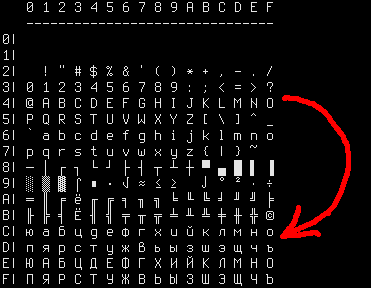
\includegraphics[width=0.5\textwidth]{fundamentals/koi8r.png}
\caption{KOI8-R table}
\end{figure}

Someone may notice that Cyrillic characters are allocated almost in the same sequence as Latin ones.
This leads to one important property: if all 8th bits in Cyrillic text encoded in KOI-8R are to be reset,
a text transforms into transliterated text with Latin characters in place of Cyrillic.
For example, Russian sentence:

\begin{framed}
\begin{quotation}
Мой дядя самых честных правил, Когда не в шутку занемог, Он уважать себя заставил, И лучше выдумать не мог.
\end{quotation}
\end{framed}

\dots if encoded in KOI-8R and then 8th bit stripped, transforms into:

\begin{framed}
\begin{quotation}
mOJ DQDQ SAMYH \^{}ESTNYH PRAWIL, kOGDA NE W [UTKU ZANEMOG, oN UWAVATX SEBQ ZASTAWIL, i LU\^{}[E WYDUMATX NE MOG.
\end{quotation}
\end{framed}

\dots perhaps this is not very appealing \ae{}sthetically, but this text is still readable to Russian language natives.

Hence, Cyrillic text encoded in KOI-8R, passed through an old 7-bit service will survive into transliterated, but still
readable text.

Stripping 8th bit is automatically transposes any character from the second half of
the (any) 8-bit \ac{ASCII} table to the first one, into the same place (take a look at red arrow right of table).
If the character has already been placed in the first half (i.e., it has been in standard 7-bit \ac{ASCII} table), it's not transposed.

Perhaps, transliterated text is still recoverable, if you'll add 8th bit to the characters which were seems
transliterated.

Drawback is obvious: Cyrillic characters allocated in KOI-8R table are not in the same sequence as
in Russian/Bulgarian/Ukrainian/etc. alphabet, and this isn't suitable for sorting, for example.

}\RU{\section{AND}

\subsection{Проверка того, находится ли значение на границе $2^n$}

Если нужно проверить, делится ли ваше значение на число вида 
$2^n$ (как 1024, 4096, итд.) без остатка,
вы можете использовать оператор \TT{\%} в \CCpp, но есть способ проще.
4096 это 0x1000, так что в нем всегда есть $4*3=12$ нулевых младших бит.

Что вам нужно, это просто:

\begin{lstlisting}[style=customc]
if (value&0xFFF)
{
	printf ("значение не делится на 0x1000 (или 4096)\n");
	printf ("кстати, остаток=%d\n", value&0xFFF);
}
else
	printf ("значение делится на 0x1000 (или 4096)\n");
\end{lstlisting}

Другими словами, это код проверяет, если здесь любой выставленный бит среди младших 12-и бит.
В качестве побочного эффекта, младщие 12 бит это всегда остаток от деления значения на 4096 (потому что деление на $2^n$
это лишь сдвиг вправо, и сдвинутые (или выброшенные) биты это биты остатка.

Та же история, если вам нужно проверить, является ли число четным или нет:

\begin{lstlisting}[style=customc]
if (value&1)
	// нечетное
else
	// четное
\end{lstlisting}

Это то же самое, как и деление на 2 и вычисление 1-битного остатка.

\subsection{Кирилличная кодировка KOI-8R}

Было время, когда 8-битная таблица \ac{ASCII} не поддерживалась некоторыми сервисами в Интернете, включая электронную почту.
Некоторые поддерживали, некоторые другие --- нет.

И это также было время, когда не-латинские системы письменности использовали вторую половину 8-битной таблицы ASCII
для размещения не-латинских символов.
Было несколько популярный кирилличных кодировок, но KOI-8R (придуманная Андреем ``ache'' Черновым)
в каком-то смысле уникальная, если сравнивать с другими.

% TODO invert arrow 
% TODO text latex form instead of png!
\begin{figure}[H]
\centering
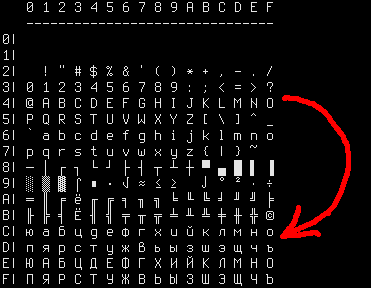
\includegraphics[width=0.5\textwidth]{fundamentals/koi8r.png}
\caption{KOI8-R table}
\end{figure}

Кое-кто может заметить, что кирилличные символы расположены почти в том же порядке, в котором и латинские.
Это приводит к важному свойству: если в кирилличном тексте закодированном в KOI-8R сбросить 8-й бит,
текст трансформируется в транслитерированный текст с латинскими символами на месте кирилличных.
Например, фраза на русском:

\begin{framed}
\begin{quotation}
Мой дядя самых честных правил, Когда не в шутку занемог, Он уважать себя заставил, И лучше выдумать не мог.
\end{quotation}
\end{framed}

\dots если закодирована в KOI-8R, и затем со сброшенным 8-м битом, трансформируется в:

\begin{framed}
\begin{quotation}
mOJ DQDQ SAMYH \^{}ESTNYH PRAWIL, kOGDA NE W [UTKU ZANEMOG, oN UWAVATX SEBQ ZASTAWIL, i LU\^{}[E WYDUMATX NE MOG.
\end{quotation}
\end{framed}

\dots конечно, выглядит это не очень эстетично, но этот текст читаем для тех, кто знает русский язык.

Следовательно, кирилличный текст закодированный в KOI-8R, пропущенный чере сервис поддерживающий только 7 бит,
выживет в виде транслитерированного, но читаемого текста.

Очистка 8-го бита автоматически транспонирует любой символ из второй половины (любой) 8-битной \ac{ASCII}-таблицы
в первую половину, в то же место (посмотрите на красную стрелку справа от таблицы).
Если символ уже расположен в первой половине (т.е., он находился в стандартной 7-битной \ac{ASCII}-таблице),
он не будет транспонироваться.

Вероятно, транслитерированный текст все еще можно восстановить, если вы прибавите 8-й бит к символам,
которые выглядят как транслитерированные.

Недостаток виден сразу: кирилличные символы расположенные в таблице KOI-8R расположены не в том порядке,
в каком они расположены в русском/болгарском/украинском/итд алфавите, и это не удобно для сортировки, например.

}

\EN{\section{AND and OR as subtraction and addition}

\subsection{ZX Spectrum ROM text strings}
\label{ZX Spectrum}

Those who once investigated ZX Spectrum \ac{ROM} internals, probably noticed that the last symbol of each text string is seemingly
absent.

\begin{figure}[H]
\centering
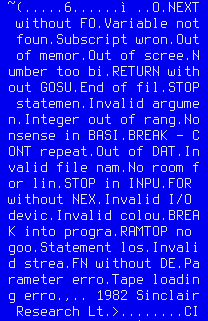
\includegraphics[width=0.3\textwidth]{fundamentals/zx_spectrum_ROM.png}
\caption{Part of ZX Spectrum ROM}
\end{figure}

There are present, in fact.

Here is excerpt of ZX Spectrum 128K ROM disassembled:

\lstinputlisting{fundamentals/ZX_Spectrum_ROM.lst}
( \url{http://www.matthew-wilson.net/spectrum/rom/128_ROM0.html} )

Last character has most significant bit set, which marks string end.
Presumably, it was done to save some space?
Old 8-bit computers has very tight environment.

Characters of all messages are always in standard 7-bit \ac{ASCII} table,
so it's guaranteed 8th bit is never used for characters.

To print such string, we must check \ac{MSB} of each byte, and if it's set, we must clear it, then print character,
and then stop.
Here is a C example:

\begin{lstlisting}[style=customc]
unsigned char hw[]=
{
	'H',
	'e',
	'l',
	'l',
	'o'|0x80
};

void print_string()
{
	for (int i=0; ;i++)
	{
		if (hw[i]&0x80) // check MSB
		{
			// clear MSB
			// (in other words, clear all, but leave 7 lower bits intact)
			printf ("%c", hw[i] & 0x7F);
			// stop
			break;
		};
		printf ("%c", hw[i]);
	};
};
\end{lstlisting}

Now what is interesting, since 8th bit is the most significant bit (in byte), we can check it, set it and remove it using
arithmetical operations instead of logical.

I can rewrite my C example:

\begin{lstlisting}[style=customc]
unsigned char hw[]=
{
	'H',
	'e',
	'l',
	'l',
	'o'+0x80
};

void print()
{
	for (int i=0; ;i++)
	{
		// hw[] must have 'unsigned char' type
		if (hw[i] >= 0x80) // check for MSB
		{
			printf ("%c", hw[i]-0x80); // clear MSB
			// stop
			break;
		};
		printf ("%c", hw[i]);
	};
};
\end{lstlisting}

By default, \IT{char} is signed type in C/C++, so to compare it with variable like 0x80 (which is negative ($-128$)
if treated as signed),
we must treat each character in text message as unsigned.

Now if 8th bit is set, the number is always larger or equal to 0x80.
If 8th bit is clear, the number is always smaller than 0x80.

Even more than that: if 8th bit is set, it can be cleared by subtracting 0x80, nothing else.
If it's not set beforehand, however, subtracting will destruct other bits.

Likewise, if 8th bit is clear, it's possible to set it by adding 0x80.
But if it's set beforehand, addition operation will destruct some other bits.

In fact, this is valid for any bit.
If the 4th bit is clear, you can set it just by adding 0x10: 0x100+0x10 = 0x110.
If the 4th bit is set, you can clear it by subtracting 0x10: 0x1234-0x10 = 0x1224.

It works, because carry isn't happened during addition/subtraction.
It will, however, happen, if the bit is already set there before addition, or absent before subtraction.

Likewise, addition/subtraction can be replaced using OR/AND operation if two conditions are met:
1) you want to add/subtract by a number in form of $2^n$;
2) this bit in source value is clear/set.

For example, addition of 0x20 is the same as ORing value with 0x20 under condition that this bit is clear before:
0x1204|0x20 = 0x1204+0x20 = 0x1224.

Subtraction of 0x20 is the same as ANDing value with ~0x20 (0x....FFDF), but if this bit is set before:
0x1234\&(\~{}0x20) = 0x1234\&0xFFDF = 0x1234-0x20 = 0x1214.

Again, it works because carry not happened when you add $2^n$ number and this bit isn't set before.

This property of boolean algebra is important, worth understanding and keeping it in mind.

}\RU{\section{\IT{И} и \IT{ИЛИ} как вычитание и сложение}

\subsection{Текстовые строки в \ac{ROM} ZX Spectrum}
\label{ZX Spectrum}

Те, кто пытался исследовать внутренности \ac{ROM} ZX Spectrum-а, вероятно, замечали,
что последний символ каждой текстовой строки как будто бы отсутствует.

\begin{figure}[H]
\centering
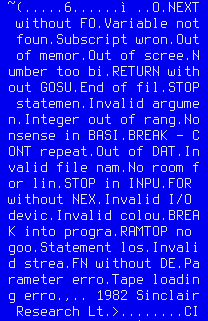
\includegraphics[width=0.3\textwidth]{fundamentals/zx_spectrum_ROM.png}
\caption{Часть \ac{ROM} ZX Spectrum}
\end{figure}

На самом деле, они присутствуют.

Вот фрагмент из дизассемблированного \ac{ROM} ZX Spectrum 128K:

\lstinputlisting{fundamentals/ZX_Spectrum_ROM.lst}
( \url{http://www.matthew-wilson.net/spectrum/rom/128_ROM0.html} )

Последний символ имеет выставленный старший бит, который означает конец строки.
Вероятно, так было сделано, чтобы сэкономить место?
В старых 8-битных компьютерах был сильный дефицит памяти.

Символы всех сообщений всегда находятся в стандартной 7-битной \ac{ASCII}-таблице, так что это гарантия,
что 8-й бит никогда не используется для символов.

Чтобы вывести такую строку, мы должны проверять \ac{MSB} каждого байта, и если он выставлен, мы должны его сбросить,
затем вывести символ, затем остановиться.
Вот пример на Си:

\begin{lstlisting}[style=customc]
unsigned char hw[]=
{
	'H',
	'e',
	'l',
	'l',
	'o'|0x80
};

void print_string()
{
	for (int i=0; ;i++)
	{
		if (hw[i]&0x80) // проверить MSB
		{
			// сбросить MSB
			// §(иными словами, сбросить всё, но оставить нетронутыми младшие 7 бит)§
			printf ("%c", hw[i] & 0x7F);
			// остановиться
			break;
		};
		printf ("%c", hw[i]);
	};
};
\end{lstlisting}

И вот что интересно, так как 8-й бит это самый старший бит (в байте), мы можем проверить его, выставить и сбросить
используя арифметические операции вместо логических.

Я могу переписать свой пример на Си:

\begin{lstlisting}[style=customc]
unsigned char hw[]=
{
	'H',
	'e',
	'l',
	'l',
	'o'+0x80
};

void print()
{
	for (int i=0; ;i++)
	{
		// hw[] должен иметь тип 'unsigned char'
		if (hw[i] >= 0x80) // проверить MSB
		{
			printf ("%c", hw[i]-0x80); // сбросить MSB
			// останов
			break;
		};
		printf ("%c", hw[i]);
	};
};
\end{lstlisting}

\IT{char} по умолчанию это знаковый тип в \CCpp, так что, чтобы сравнивать его с переменной вроде 0x80 (которая отрицательная
($-128$),
если считается за знаковую),
мы должны считать каждый символ сообщения как беззнаковый.

Теперь, если 8-й бит выставлен, число всегда больше или равно 0x80.
Если 8-й бит сброшен, число всегда меньше 0x80.

И даже более того: если 8-й бит выставлен, его можно сбросить вычитанием 0x80, и ничего больше.
Если он уже сброшен, впрочем, операция вычитания уничтожит другие биты.

Точно также, если 8-й бит сброшен, можно его выставить прибавлением 0x80.
Но если он уже выставлен, операция сложения уничтожит остальные биты.

На самом деле, это справедливо для любого бита.
Если 4-й бит сброшен, вы можете выставить его просто прибавлением 0x10: 0x100+0x10 = 0x110.
Если 4-й бит выставлен, вы можете его сбросить вычитанием 0x10: 0x1234-0x10 = 0x1224.

Это работает, потому что перенос не случается во время сложения/вычитания.
Хотя, он случится если бит уже выставлен перед сложением или сброшен перед вычитанием.

Точно также, сложение/вычитание можно заменить на операции \IT{ИЛИ/И} если справедливы два условия:
1) вы хотите прибавить/вычесть число вида $2^n$;
2) бит в исходном значение сброшен/выставлен.

Например, прибавление 0x20 это то же что и применение \IT{ИЛИ} со значением 0x20 с условием что этот бит был сброшен перед
этим:
0x1204|0x20 = 0x1204+0x20 = 0x1224.

Вычитание 0x20 это то же что и применение \IT{И} со значением ~0x20 (0x....FFDF), но если этот бит был выставлен до этого:
0x1234\&(\~{}0x20) = 0x1234\&0xFFDF = 0x1234-0x20 = 0x1214.

Опять же, это работает потому что перенос не случается если вы прибавляете число вида $2^n$ и этот бит до этого сброшен.

Это важное свойство булевой алгербы, его стоит понимать и помнить о нем.

}

\EN{\section{XOR (exclusive OR)}
\label{XOR_property}

\input{fundamentals/XOR_property_EN}

\subsection{Everyday speech}

XOR operation present in common everyday speech.
When someone asks ``please buy apples or bananas'',
this usually means ``buy the first object or the second, but not both''---this is exactly exclusive OR,
because logical OR would mean ``both objects are also fine''.

Some people suggest ``and/or'' should be used in everyday speech to make emphasis that logical OR is used instead of
exclusive OR: \url{https://en.wikipedia.org/wiki/And/or}.

\subsection{Encryption}

XOR is heavily used in both amateur (\ref{simple_XOR_encryption}) and \IT{real} encryption (at least in \IT{Feistel network}).

XOR is very useful here because:
$cipher\_text = plain\_text \oplus key$ and then:
$(plain\_text \oplus key) \oplus key = plain\_text$.

\subsection{\ac{RAID}4}
\index{RAID4}

\ac{RAID}4 offers a very simple method to to protect hard disks.
For example, there are several disks ($D_1$, $D_2$, $D_3$, etc.) and one parity disk ($P$).
Each bit/byte written to parity disk is calculated and written on-fly:

\begin{equation} \label{eq:RAID4}
P = D_1 \oplus D_2 \oplus D_3
\end{equation}

If any of disks is failed, for example, $D_2$, it's restored using the very same way:

\begin{equation}
D_2 = D_1 \oplus P \oplus D_3
\end{equation}

If parity disk failed, it is restored using \ref{eq:RAID4} way.
If two of any disks are failed, then it wouldn't be possible to restore both.

\ac{RAID}5 is more advanced, but this XOR property is still exploited there.

That's why \ac{RAID} controllers has hardware ``XOR accelerators'' helping to XOR large chunks of written data on-fly.
When computers get faster and faster, it now can be done at software level, using \ac{SIMD}.

\subsection{XOR swap algorithm}

Hard to believe, but this code swaps values in \EAX and \EBX without aid of any other additional register or memory cell:

\begin{lstlisting}[style=customasmx86]
xor eax, ebx
xor ebx, eax
xor eax, ebx
\end{lstlisting}

Let's find out, how it works.
First, we will rewrite it to step aside from x86 assembly language:

\begin{lstlisting}
X = X XOR Y
Y = Y XOR X
X = X XOR Y
\end{lstlisting}

What X and Y has at each step?
Just keep in mind the simple rule: $(X \oplus Y) \oplus Y = X$ for any values of X and Y.

Let's see,
$X$ after 1st step has $X \oplus Y$;
$Y$ after 2nd step has $Y \oplus (X \oplus Y) = X$;
$X$ after 3rd step has $(X \oplus Y) \oplus X = Y$.

Hard to say if anyone should use this trick, but it servers as a good demonstration example of XOR properties.

Wikipedia article (\url{https://en.wikipedia.org/wiki/XOR_swap_algorithm}) has also yet another explanation:
addition and subtraction operations can be used instead of XOR:

\begin{lstlisting}
X = X + Y
Y = X - Y
X = X - Y
\end{lstlisting}

Let's see:
$X$ after 1st step has $X+Y$;
$Y$ after 2nd step has $X+Y-Y=X$;
$X$ after 3rd step has $X+Y-X=Y$.

\subsection{XOR linked list}
\index{Doubly linked list}

Doubly linked list is a list in which each element has link to the previous element and to the next one.
Hence, it's very easy to traverse list backwards or forward.
\TT{std::list} in C++ implements doubly linked list which also is examined in this book: \ref{std_list}.

So each element has two pointers.
Is it possible, perhaps in environment of small \ac{RAM} footprint, to preserve all functionality with one pointer instead of two?
Yes, if it a value of $prev \oplus next$ will be stored in this memory cell, which is usually called ``link''.

Maybe, we could say that address to the previous element is ``encrypted'' using address of next element and otherwise:
next element address is ``encrypted'' using previous element address.

When we traverse this list forward, we always know address of the previous element, so we can ``decrypt'' this field and get 
address of the next element.
Likewise, it's possible to traverse this list backwards, ``decrypting'' this field using next element's address.

But it's not possible to find address of previous or next element of some specific element without
knowing address of the first one.

Couple of things to complete this solution: first element will have address of next element without any XOR-ing,
last element will have address of previous element without any XOR-ing.

Now let's sum it up. This is example of doubly linked list of 5 elements.
$A_x$ is address of element.

\begin{center}
\begin{tabular}{ | l | l | }
	\hline
	\HeaderColor address & \HeaderColor \IT{link} field contents \\
	\hline
	$A_0$ & $A_1$ \\
	\hline
	$A_1$ & $A_0 \oplus A_2$ \\
	\hline
	$A_2$ & $A_1 \oplus A_3$ \\
	\hline
	$A_3$ & $A_2 \oplus A_4$ \\
	\hline
	$A_4$ & $A_3$ \\
	\hline
\end{tabular}
\end{center}

And again, hard to say if anyone should use this tricky hacks, but this is also a good demonstration of XOR properties.
As with XOR swap algorithm, Wikipedia article about it also offers way to use addition or subtraction instead of XOR:
\url{https://en.wikipedia.org/wiki/XOR_linked_list}.

\subsection{By the way}

The usual \IT{OR} also sometimes called \IT{inclusive OR} (or even \IT{IOR}), as opposed to \IT{exclusive OR}.

}\RU{\section{XOR (исключающее \IT{ИЛИ})}
\label{XOR_property}

\input{fundamentals/XOR_property_RU}

\subsection{Бытовая речь}

Оперция XOR присутствует в обычной бытовой речи.
Когда кто-то просит ``пожалуйста, купи яблок или бананов'',
это обычно означает ``купи первый объект, или второй, но не оба'' --- это и есть исключающее ИЛИ,
потому что логическое ИЛИ означало бы ``оба объекта тоже сгодятся''.

Некоторые люди предлагают использовать в речи ``и/или'', чтобы подчеркнуть тот факт, что используется именно логическое ИЛИ
вместо исключающего ИЛИ: \url{https://en.wikipedia.org/wiki/And/or}.

\subsection{Шифрование}

Исключающее ИЛИ много используется как в любительской криптографии (\ref{simple_XOR_encryption}), так и в \IT{настоящей}
(как минимум в \IT{сети Фестеля}).

Эта операция очень удобна потому что:
\IT{шифрованный\_текст = исходный\_текст $\oplus$ ключ} и затем:
\IT{(исходный\_текст $\oplus$ ключ) $\oplus$ ключ = исходный\_текст}.

\subsection{\ac{RAID}4}
\index{RAID4}

\ac{RAID}4 предлагает очень простой метод защиты жестких дисков.
Например, есть несколько дисков ($D_1$, $D_2$, $D_3$, итд.) и один диск чётности (\IT{parity disk}) ($P$).
Каждый бит/байт записываемый на диск чётности вычисляется на лету:

\begin{equation} \label{eq:RAID4}
P = D_1 \oplus D_2 \oplus D_3
\end{equation}

Если один из дисков испортился, например, $D_2$, он восстанавливается точно также:

\begin{equation}
D_2 = D_1 \oplus P \oplus D_3
\end{equation}

Если диск чётности испортился, он восстанавливается так же: \ref{eq:RAID4}.
Если два любых диска испортились, тогда уже не получится восстановить оба.

\ac{RAID}5 развился далее, но эта особенность исключающего ИЛИ используется и там.

Вот почему в контроллерах \ac{RAID} были ``XOR-акселлераторы'', они помогали XOR-ить большие объемы данных
на лету, перед записью на диски.
Когда компьютеры стали быстрее, стало возможным делать это же программно, используя \ac{SIMD}.

\subsection{Алгоритм обмена значений при помощи исключающего ИЛИ}

Трудно поверить, но этот код меняет значения в \EAX и \EBX без помощи вспомогательного регистра или ячейки памяти:

\begin{lstlisting}[style=customasmx86]
xor eax, ebx
xor ebx, eax
xor eax, ebx
\end{lstlisting}

Посмотрим, как это работает.
Для начала, мы перепишем этот код, чтобы отойти от ассемблера x86:

\begin{lstlisting}
X = X XOR Y
Y = Y XOR X
X = X XOR Y
\end{lstlisting}

Что содержат X и Y на каждом шаге?
Просто держите в памяти простое правило: $(X \oplus Y) \oplus Y = X$ для любых значений X и Y.

Посмотрим,
$X$ после первого шага это $X \oplus Y$;
$Y$ после второго шага это $Y \oplus (X \oplus Y) = X$;
$X$ после третьего шага это $(X \oplus Y) \oplus X = Y$.

Трудно сказать, стоит ли использовать этот трюк, но он служит неплохой демонстрацией свойств исключающего ИЛИ.

В статье Wikipedia (\url{https://en.wikipedia.org/wiki/XOR_swap_algorithm}) есть еще такое объяснение:
можно использовать сложение и вычитание вместо исключающего ИЛИ:

\begin{lstlisting}
X = X + Y
Y = X - Y
X = X - Y
\end{lstlisting}

Посмотрим:
$X$ после первого шага это $X+Y$;
$Y$ после второго шага это $X+Y-Y=X$;
$X$ после третьего шага это $X+Y-X=Y$.

\subsection{Список связанный при помощи XOR}
\index{Doubly linked list}

Двусвязный список это список, в котором каждый элемент имеет ссылку на предыдущий элемент и на следующий.
Следовательно, легко перечислять элементы и вперед и назад.
\TT{std::list} в Си++ реализует двусвязный список, и он рассматривается в этой книге: \ref{std_list}.

Так что каждый элемент имеет два указателя.
Возможно ли, вероятно, в среде где нужно экономить \ac{RAM}, сохранить всю функциональность используя один указатель
вместо двух?
Да, если будем хранить значение $предыдущий \oplus следующий$ в ячейке, которую обычно называют ``link''.

Можно быть, мы можем сказать, что адрес предыдущего элемента ``зашифрован'' используя адрес следующего элемента и наоборот:
адрес следующего элемента ``зашифрован'' используя адрес предыдущего элемента.

Когда мы проходим по списку вперед, мы всегда знаем адрес предыдущего элемента, так что мы можем ``расшифровать'' это поле
и получить адрес следующего элемента.
Точно также, мы можем пройти по списку назад, ``дешифруя'' это поле используя адрес следующего элемента.

Но невозможно найти адрес предыдущего или следующего элемента определенного элемента без знания адреса первого элемента.

Еще кое-что: первый элемент будем иметь адрес следующего элемента без ничего,
последний элемент будет иметь адрес предыдущего элемента без ничего.

Подведем итоги. Это пример двусвязного списка из 5-и элементов.
$A_x$ это адрес элемента.

\begin{center}
\begin{tabular}{ | l | l | }
	\hline
	\HeaderColor адрес & \HeaderColor содержимое поля \IT{link} \\
	\hline
	$A_0$ & $A_1$ \\
	\hline
	$A_1$ & $A_0 \oplus A_2$ \\
	\hline
	$A_2$ & $A_1 \oplus A_3$ \\
	\hline
	$A_3$ & $A_2 \oplus A_4$ \\
	\hline
	$A_4$ & $A_3$ \\
	\hline
\end{tabular}
\end{center}

И снова, трудно сказать, нужно ли использовать эти хаки, но это также хорошая демонстрация особенностей исключающего ИЛИ.
Как и с алгоритмом обмена значений при помощи исключающего ИЛИ, в статье Wikipedia есть также предложение использовать
сложение или вычитание вместо исключающего ИЛИ:
\url{https://en.wikipedia.org/wiki/XOR_linked_list}.

\subsection{Кстати}

Обычное \IT{ИЛИ} иногда называют \IT{включающее ИЛИ} (\IT{inclusive OR}, или даже \IT{IOR}),
чтобы противопоставить его \IT{исключающему ИЛИ}.

}

\EN{\subsection{AND/OR/XOR as MOV}

\INS{OR reg, 0xFFFFFFFF} sets all bits to 1, hence, no matter what has been in register before, it will be set to $-1$.
\INS{OR reg, -1} is shorter than \INS{MOV reg, -1}, so MSVC uses OR instead the latter,
for example: \myref{using_OR_instead_of_MOV}.

Likewise, \INS{AND reg, 0} always resets all bits, hence, it acts like \INS{MOV reg, 0}.

\INS{XOR reg, reg}, no matter what has been in register beforehand, resets all bits, and also acts like \INS{MOV reg, 0}.

}
\ES{
\subsection{AND/OR/XOR como MOV}

\INS{OR reg, 0xFFFFFFFF} establece todos los bits a 1, por lo tanto, no importa lo que estaba antes en el registro, este ser\'a establecido a $-1$.
\INS{OR reg, -1} es m\'as corto que \INS{MOV reg, -1}, as\'í que MSVC usa el OR en vez del MOV.

por ejemplo \myref{using_OR_instead_of_MOV}.

As\'i, \INS{AND reg, 0} siempre resetea todos los bits, por lo tanto, act\'ua como un \INS{MOV reg, 0}.

\INS{XOR reg, reg}, resetea todos los bits, sin importar lo que estuviese antes en el registro, y tambi\'en es quivalente a un \INS{MOV reg, 0}.
}
\RU{\subsection{AND/OR/XOR как MOV}

Инструкция \INS{OR reg, 0xFFFFFFFF} выставляет все биты в 1, следовательно, не важно что было в регистре перед этим,
его значение будет выставлено в $-1$.
Инструкция \INS{OR reg, -1} короче, чем \INS{MOV reg, -1}, так что MSVC использует OR вместо последней,
например: \myref{using_OR_instead_of_MOV}.

Точно также, \INS{AND reg, 0} всегда сбрасывает все биты, следовательно, работает как \INS{MOV reg, 0}.

\INS{XOR reg, reg}, не важно что было в регистре перед этим, сбрасывает все биты, и также работает как \INS{MOV reg, 0}.

}

\EN{\section{Population count}
\label{POPCNT}

\INS{POPCNT} instruction is population count (\ac{AKA} Hamming weight).
It just counts number of bits set in an input value.

As a side effect, \INS{POPCNT} instruction (or operation) can be used to determine, if the value has $2^n$ form.
Since, $2^n$ number always has just one single bit, \INS{POPCNT}'s result will always be just 1.

\myindex{base64scanner}
For example, I once wrote a base64 strings scanner for hunting something interesting in binary files\footnote{\url{https://github.com/dennis714/base64scanner}}.
And there is a lot of garbage and false positives, so I add an option to filter out data blocks which has size of $2^n$ bytes
(i.e., 256 bytes, 512, 1024, etc.).
The size of block is checked just like this:

\begin{lstlisting}[style=customc]
if (popcnt(size)==1)
	// OK
...
\end{lstlisting}

The instruction is also known as \q{\ac{NSA} instruction} due to rumors:

\begin{framed}
\begin{quotation}
  This branch of cryptography is fast-paced and very politically charged.
  Most designs are secret; a majority of military encryptions systems in use today are 
  based on LFSRs. 
  In fact, most Cray computers (Cray 1, Cray X-MP, Cray Y-MP) have a rather curious 
  instruction generally known as “population count.” It counts the 1 bits in a register 
  and can be used both to efficiently calculate the Hamming distance between two binary 
  words and to implement a vectorized version of a LFSR. I’ve heard this called the canonical 
  NSA instruction, demanded by almost all computer contracts.
\end{quotation}
\end{framed}
\InSqBrackets{\Schneier{}}

}\RU{\section{Подсчет бит}
\label{POPCNT}

Инструкция \INS{POPCNT} (\IT{population count}) служит для подсчета бит во входном значении (\ac{AKA} расстояние Хэмминга).

В качестве побочного эффекта, инструкция \INS{POPCNT} (или операция) может использоваться, чтобы узнать,
имеет ли значение вид $2^n$.
Так как числа $2^n$ всегда имеют только один выставленный бит, результат \INS{POPCNT} всегда будет просто 1.

\myindex{base64scanner}
Например, я однажды написал сканер для поиска base64-строк в бинарных файлах\footnote{\url{https://github.com/dennis714/base64scanner}}.
И есть много мусора и ложных срабатываний, так что я добавил опцию для фильтрования блоков данных, размер которых $2^n$ байт
(т.е., 256 байт, 512, 1024, итд.).
Размер блока проверяется так:

\begin{lstlisting}[style=customc]
if (popcnt(size)==1)
	// OK
...
\end{lstlisting}

Инструкция также известна как \q{инструкция \ac{NSA}} из-за слухов:

\begin{framed}
\begin{quotation}
  This branch of cryptography is fast-paced and very politically charged.
  Most designs are secret; a majority of military encryptions systems in use today are 
  based on LFSRs. 
  In fact, most Cray computers (Cray 1, Cray X-MP, Cray Y-MP) have a rather curious 
  instruction generally known as “population count.” It counts the 1 bits in a register 
  and can be used both to efficiently calculate the Hamming distance between two binary 
  words and to implement a vectorized version of a LFSR. I’ve heard this called the canonical 
  NSA instruction, demanded by almost all computer contracts.
\end{quotation}
\end{framed}
\InSqBrackets{\Schneier{}}

}

\EN{\section{Endianness}
\label{sec:endianness}

The endianness is a way of representing values in memory.

\subsection{Big-endian}

The \TT{0x12345678} value is represented in memory as:

\begin{center}
\begin{tabular}{ | l | l | }
\hline
\HeaderColor address in memory & \HeaderColor byte value \\
\hline
+0 & 0x12 \\
\hline
+1 & 0x34 \\
\hline
+2 & 0x56 \\
\hline
+3 & 0x78 \\
\hline
\end{tabular}
\end{center}

Big-endian CPUs include Motorola 68k, IBM POWER.

\subsection{Little-endian}

The \TT{0x12345678} value is represented in memory as:

\begin{center}
\begin{tabular}{ | l | l | }
\hline
\HeaderColor address in memory & \HeaderColor byte value \\
\hline
+0 & 0x78 \\
\hline
+1 & 0x56 \\
\hline
+2 & 0x34 \\
\hline
+3 & 0x12 \\
\hline
\end{tabular}
\end{center}

Little-endian CPUs include Intel x86.

\subsection{\Example}

Let's take big-endian MIPS Linux installed and ready in QEMU
\footnote{Available for download here: \url{http://go.yurichev.com/17008}}.

And let's compile this simple example:

\begin{lstlisting}[style=customc]
#include <stdio.h>

int main()
{
	int v, i;

	v=123;

	printf ("%02X %02X %02X %02X\n", 
		*(char*)&v,
		*(((char*)&v)+1),
		*(((char*)&v)+2),
		*(((char*)&v)+3));
};
\end{lstlisting}

After running it we get:

\begin{lstlisting}
root@debian-mips:~# ./a.out 
00 00 00 7B
\end{lstlisting}

That is it.
0x7B is 123 in decimal.
In little-endian architectures, 7B is the first byte (you can check on x86 or x86-64), 
but here it is the last one, because the highest byte goes first.

That's why there are separate Linux distributions for MIPS
(\q{mips} (big-endian) and \q{mipsel} (little-endian)).
It is impossible for a binary compiled for one endianness to work on an \ac{OS} with different endianness. 

There is another example of MIPS big-endiannes in this book: \myref{MIPS_structure_big_endian}.

\subsection{Bi-endian}

CPUs that may switch between endianness are ARM, PowerPC, SPARC, MIPS, \ac{IA64}, etc.

\subsection{Converting data}

\myindex{x86!\Instructions!BSWAP}
The \TT{BSWAP} instruction can be used for conversion.

\myindex{TCP/IP}
TCP/IP network data packets use the big-endian conventions, so that is why a program working on a little-endian architecture
has to convert the values.
The \TT{htonl()} and \TT{htons()} functions are usually used.

In TCP/IP, big-endian is also called \q{network byte order}, while byte order on the computer \q{host byte order}.
\q{host byte order} is little-endian on Intel x86 and other little-endian architectures,
but it is big-endian on IBM POWER, so \TT{htonl()} and \TT{htons()} don't shuffle any bytes on the latter.

}\ES{\section{Endianness}
\label{sec:endianness}

Endianness es una forma de representar valores en la memoria.

\subsection{Big-endian}

El valor \TT{0x12345678} es representado en la memoria como:

\begin{center}
\begin{tabular}{ | l | l | }
\hline
\HeaderColor direcci\'on en memoria & \HeaderColor valor del byte \\
\hline
+0 & 0x12 \\
\hline
+1 & 0x34 \\
\hline
+2 & 0x56 \\
\hline
+3 & 0x78 \\
\hline
\end{tabular}
\end{center}

Entre los CPU big-endian se encuentran Motorola 68k, IBM POWER.

\subsection{Little-endian}

El valor \TT{0x12345678} es representado en la memoria como:

\begin{center}
\begin{tabular}{ | l | l | }
\hline
\HeaderColor Direcci\'on en memoria & \HeaderColor valor del byte \\
\hline
+0 & 0x78 \\
\hline
+1 & 0x56 \\
\hline
+2 & 0x34 \\
\hline
+3 & 0x12 \\
\hline
\end{tabular}
\end{center}

Entre los CPU little-endian tenemos el Intel x86.

\subsection{\Example}

Tomemos el MIPS big-endian para Linux instalado y listo en QEMU
\footnote{Disponible para descargar aqu\'i: \url{http://go.yurichev.com/17008}%}.

Y compilemos este ejemplo sencillo:

\begin{lstlisting}[style=customc]
#include <stdio.h>

int main()
{
	int v, i;

	v=123;

	printf ("%02X %02X %02X %02X\n", 
		*(char*)&v,
		*(((char*)&v)+1),
		*(((char*)&v)+2),
		*(((char*)&v)+3));
};
\end{lstlisting}

Despu\'es de correrlo obtenemos:

\begin{lstlisting}
root@debian-mips:~# ./a.out 
00 00 00 7B
\end{lstlisting}

Eso es todo.
0x7B es 123 en decimal.
En las arquitecturas little-endian, 7B es el primer byte (puedes checarlo en x86 o x86-64),
pero aqu\'i es el \'ultimo, porque el byte m\'as alto va primero.

Por eso hay distribuciones separadas de Linux para MIPS
(\q{mips} (big-endian) \ESph{} \q{mipsel} (little-endian)).
Es imposible que un binario compilado para un endianness trabaje en un SO con diferente endianness.

En este libro hay otro ejemplo de big-endianness en MIPS: \myref{MIPS_structure_big_endian}.

\subsection{Bi-endian\RU{ (переключаемый порядок)}}

CPUs que puede cambiar entre endianness son ARM, PowerPC, SPARC, MIPS, \ac{IA64}, etc.

\subsection{Convirtiendo datos}

\myindex{x86!\Instructions!BSWAP}
La instrucci\'on \TT{BSWAP} puede ser utilizada para conversiones.

\myindex{TCP/IP}
Los paquetes de datos en redes TCP/IP utilizan convenciones big-endian, por eso un programa corriendo en una arquitectura
little-endian tiene que convertir los valores.

Las funciones \TT{htonl()} \ESph{} \TT{htons()} son usadas generalmente.

En TCP/IP, big-endian tambi\'en es llamado \q{orden de bytes de red},
mientras que el orden de bytes en la computadora se conoce como \q{orden de bytes de host}.
\q{orden de bytes de host} es little-endian en Intel x86 y otras arquitecturas little-endian,
pero es big-endian en IBM POWER, asi que \TT{htonl()} y \TT{htons()} no cambian el orden de los bytes
en \'esta \'ultima.

}\RU{\section{Endianness (порядок байт)}
\label{sec:endianness}

Endianness (порядок байт) это способ представления чисел в памяти.

\subsection{Big-endian (от старшего к младшему)}

Число \TT{0x12345678} представляется в памяти так:

\begin{center}
\begin{tabular}{ | l | l | }
\hline
\HeaderColor адрес в памяти & \HeaderColor значение байта \\
\hline
+0 & 0x12 \\
\hline
+1 & 0x34 \\
\hline
+2 & 0x56 \\
\hline
+3 & 0x78 \\
\hline
\end{tabular}
\end{center}

CPU с таким порядком включают в себя Motorola 68k, IBM POWER.

\subsection{Little-endian (от младшего к старшему)}

Число \TT{0x12345678} представляется в памяти так:

\begin{center}
\begin{tabular}{ | l | l | }
\hline
\HeaderColor адрес в памяти & \HeaderColor значение байта \\
\hline
+0 & 0x78 \\
\hline
+1 & 0x56 \\
\hline
+2 & 0x34 \\
\hline
+3 & 0x12 \\
\hline
\end{tabular}
\end{center}

CPU с таким порядком байт включают в себя Intel x86.

\subsection{\Example}

Возьмем big-endian Linux для MIPS заинсталированный в QEMU
\footnote{Доступен для скачивания здесь: \url{http://go.yurichev.com/17008}}.

И скомпилируем этот простой пример:

\begin{lstlisting}[style=customc]
#include <stdio.h>

int main()
{
	int v, i;

	v=123;

	printf ("%02X %02X %02X %02X\n", 
		*(char*)&v,
		*(((char*)&v)+1),
		*(((char*)&v)+2),
		*(((char*)&v)+3));
};
\end{lstlisting}

И запустим его:

\begin{lstlisting}
root@debian-mips:~# ./a.out 
00 00 00 7B
\end{lstlisting}

Это оно и есть.
0x7B это 123 в десятичном виде.
В little-endian-архитектуре, 7B это первый байт (вы можете это проверить в x86 или x86-64),
но здесь он последний, потому что старший байт идет первым.

Вот почему имеются разные дистрибутивы Linux для MIPS
(\q{mips} (big-endian) и \q{mipsel} (little-endian)).
Программа скомпилированная для одного соглашения об endiannes, не сможет работать в OS использующей
другое соглашение.

Еще один пример связанный с big-endian в MIPS в этой книге: \myref{MIPS_structure_big_endian}.

\subsection{Bi-endian (переключаемый порядок)}

CPU поддерживающие оба порядка, и его можно переключать, включают в себя ARM, PowerPC, SPARC, MIPS, \ac{IA64}, итд.

\subsection{Конвертирование}

\myindex{x86!\Instructions!BSWAP}
Инструкция \TT{BSWAP} может использоваться для конвертирования.

\myindex{TCP/IP}
Сетевые пакеты TCP/IP используют соглашение big-endian, вот почему программа, работающая на little-endian архитектуре
должна конвертировать значения.

Обычно, используются функции \TT{htonl()} и \TT{htons()}.

Порядок байт big-endian в среде TCP/IP также называется, \q{network byte order},
а порядок байт на компьютере \q{host byte order}.
На архитектуре Intel x86, и других little-endian архитектурах, \q{host byte order} это little-endian, 
а вот на IBM POWER это может быть big-endian, так что на последней, 
\TT{htonl()} и \TT{htons()} не меняют порядок байт.

}

\EN{\section{Memory}

There are 3 main types of memory:

\begin{itemize}
\item
Global memory \ac{AKA} \q{static memory allocation}.
No need to allocate explicitly, the allocation is performed just by declaring variables/arrays 
globally.
These are global variables, residing in the data or constant segments.
They are available globally (hence, considered as an \gls{anti-pattern}).
Not convenient for buffers/arrays, because they must have a fixed size.
Buffer overflows that occur here usually overwrite variables or buffers residing next to them in memory.
There's an example in this book: \myref{scanf_global_variable}.

\item
Stack \ac{AKA} \q{allocate on stack}.
The allocation is performed just by declaring variables/arrays locally in the function.
These are usually local variables for the function.
Sometimes these local variable are also available to descending functions 
(to \gls{callee} functions, if caller passes a pointer to a variable to the \gls{callee} to be executed).
Allocation and deallocation are very fast, it just \ac{SP} needs to be shifted.
\myindex{\CStandardLibrary!alloca()}

But they're also not convenient for buffers/arrays, because the buffer size has to be fixed,
unless \TT{alloca()} (\myref{alloca}) (or a variable-length array) is used.
Buffer overflows usually overwrite important stack structures: \myref{subsec:bufferoverflow}.

\myindex{\CStandardLibrary!malloc()}
\myindex{\CStandardLibrary!free()}
\item
Heap \ac{AKA} \q{dynamic memory allocation}.
Allocation/deallocation is performed by calling \\
\TT{malloc()/free()} or \TT{new/delete} in \Cpp.
This is the most convenient method: the block size may be set at runtime.
\myindex{\CStandardLibrary!realloc()}

Resizing is possible (using \TT{realloc()}), but can be slow.
This is the slowest way to allocate memory: 
the memory allocator must support and update all control structures while
allocating and deallocating.
Buffer overflows usually overwrite these structures.
Heap allocations are also source of memory leak problems: each memory block has to be deallocated
explicitly, but one may forget about it, or do it incorrectly.
\myindex{\CStandardLibrary!free()}

Another problem is the \q{use after free}---using a memory block after \TT{free()} has been called on it,
which is very dangerous.

Example in this book: \myref{struct_malloc_example}.

\end{itemize}
}\ES{% TODO probably needs to be resynchronized with EN version
\section{Memoria}

Existen 3 tipos principales de memoria:

\begin{itemize}
\item
Memoria global \ac{AKA} \q{asignaci\'on est\'atica de memoria}.
No hay necesidad de asignarla expl\'icitamente, la asignaci\'on es realizada al declarar
variables/arreglos globales.
Estas variables globales residen en los segmentos de datos o de constantes.
Est\'an disponibles globalmente (por lo tanto, se consideran un anti-patr\'on).
No son convenientes para buffers/arreglos porque deben tener un tama\~no fijo.
Los desbordamientos de buffer que occurren aqu\'i usualmente sobreescriben variables o buffers que residen
junto a ellos en memoria.
En este libro hay un ejemplo: \myref{scanf_global_variable}.

\item
Pila \ac{AKA} \q{asignaci\'on en pila}.
La asignaci\'on se realiza al declarar variables/arreglos dentro de una funci\'on.
Son usualmente variables locales a la funci\'on.
Algunas veces estas variables locales tambi\'en estan disponibles para funciones descendientes
(funciones llamadas, si aquel que la llama le pasa un apuntador a una de sus variables).
La asignaci\'on y desasignaci\'on son muy r\'apidas, s\'olo necesita que \ac{SP} sea ajustado.
\myindex{\CStandardLibrary!alloca()}
\ESph{}
Los desbordamientos de buffer suelen reescribir estructuras importantes en la pila: \myref{subsec:bufferoverflow}.

\myindex{\CStandardLibrary!malloc()}
\myindex{\CStandardLibrary!free()}
\item
Heap \ac{AKA} \q{asignaci\'on din\'amica de memoria}.
La asignaci\'on/desasignaci\'on es realizada llamando a \\
\TT{malloc()/free()} \ESph{} \TT{new/delete} \ESph{} \Cpp.
\'Este es el m\'etodo m\'as conveniente: el tama\~no del bloque puede establecerse en tiempo de ejecuci\'on.
\myindex{\CStandardLibrary!realloc()}
Cambiar el tama\~no es posible (usando \TT{realloc()}), pero puede ser lento.
\'Esta es la forma m\'as lenta de asignar memoria:
el asignador de memoria debe suportar y actualizar todas las estructuras de control
mientras se asigna y desasigna.
Los desbordamientos de buffer suelen sobreescribir estas estructuras.
Las asiganciones en el heap tambi\'en son el origen de problemas de fuga de memoria: cada bloque de memoria tiene
que ser desasgnado expl\'icitamente, pero uno puede olvidarse de ello, o hacerlo de manera incorrecta.
\myindex{\CStandardLibrary!free()}
Otro problema es el \q{uso despu\'es de la liberaci\'on}---usar un bloque de memoria despu\'es
de que \TT{free()} ha sido llamado en \'el, lo cual es muy peligroso.
Un ejemplo en este libro:
\myref{struct_malloc_example}.

\end{itemize}
}\RU{\section{Память}

Есть три основных типа памяти:

\begin{itemize}
\item
Глобальная память \ac{AKA} \q{static memory allocation}.
Нет нужды явно выделять, выделение происходит просто при объявлении переменных/массивов 
глобально.
Это глобальные переменные расположенные в сегменте данных или констант.
Доступны глобально (поэтому считаются \glslink{anti-pattern}{анти-паттерном}).
Не удобны для буферов/массивов, потому что должны иметь фиксированный размер.
Переполнения буфера, случающиеся здесь, обычно перезаписывают переменные или буферы
расположенные рядом в памяти.
Пример в этой книге: \myref{scanf_global_variable}.

\item
Стек \ac{AKA} \q{allocate on stack}, \q{выделить память в/на стеке}.
Выделение происходит просто при объявлении переменных/массивов локально в функции.%
Обычно это локальные для функции переменные.
Иногда эти локальные переменные также доступны и для нисходящих функций (\gls{callee}-функциям, если функция-\gls{caller} передает
указатель на переменную в функцию-\gls{callee}).
Выделение и освобождение очень быстрое, достаточно просто сдвига \ac{SP}.

\myindex{\CStandardLibrary!alloca()}
Но также не удобно для буферов/массивов, потому что размер буфера фиксирован,
если только не используется \TT{alloca()} (\myref{alloca}) (или массив с переменной длиной).

Переполнение буфера обычно перезаписывает важные структуры стека: \myref{subsec:bufferoverflow}.

\myindex{\CStandardLibrary!malloc()}
\myindex{\CStandardLibrary!free()}
\item
Куча (\IT{heap}) \ac{AKA} \q{dynamic memory allocation}, \q{выделить память в куче}.
Выделение происходит при помощи вызова \\
\TT{malloc()/free()} или \TT{new/delete} в \Cpp.

Самый удобный метод: размер блока может быть задан во время исполнения.
\myindex{\CStandardLibrary!realloc()}
Изменение размера возможно (при помощи \TT{realloc()}), но может быть медленным.

Это самый медленный метод выделения памяти: аллокатор памяти должен поддерживать и обновлять
все управляющие структуры во время выделения и освобождения.
Переполнение буфера обычно перезаписывает все эти структуры.
Выделения в куче также ведут к проблеме утечек памяти: каждый выделенный блок должен быть
явно освобожден, но кто-то может забыть об этом, или делать это неправильно.
\myindex{\CStandardLibrary!free()}
Еще одна проблема --- это \q{использовать после освобождения} --- использовать блок памяти после
того как \TT{free()} был вызван на нем, это тоже очень опасно.
Пример в этой книге:
\myref{struct_malloc_example}.

\end{itemize}
}

\EN{\section{CPU}

\subsection{Branch predictors}
\label{branch_predictors}

Some latest compilers try to get rid of conditional jump instructions.
Examples in this book are: \myref{subsec:jcc_ARM}, \myref{chap:cond}, \myref{subsec:popcnt}.

This is because the branch predictor is not always perfect, so the compilers try to do 
without conditional jumps, if possible.

\myindex{x86!\Instructions!CMOVcc}
\myindex{ARM!\Instructions!ADRcc}
Conditional instructions in ARM (like ADRcc) are one way, another one is the CMOVcc x86 instruction.

\subsection{Data dependencies}

Modern CPUs are able to execute instructions simultaneously (\ac{OOE}), but in order to do so,
the results of one instruction in a group must not influence the execution of others.
Hence, the compiler endeavors to use instructions with minimal influence on the CPU state.

\myindex{ARM!\Instructions!LEA}
That's why the \LEA instruction is so popular, because it does not modify CPU flags, while
other arithmetic instructions does.
}\ES{\section{CPU}

\subsection{Predictores del saltos}
\label{branch_predictors}

Algunos compiladores modernos intentan deshacerse de las instrucciones de saltos condicionales.
Ejemplos en este libro son: \myref{subsec:jcc_ARM}, \myref{chap:cond}, \myref{subsec:popcnt}.

Esto se debe a que el predictor de saltos no siempre es perfecto, por lo tanto los compiladores
tratan de evitar los saltos condicionales, de ser posible.

\myindex{x86!\Instructions!CMOVcc}
\myindex{ARM!\Instructions!ADRcc}
Las instrucciones condicionales en ARM (como ADRcc) son una forma de hacerlo, otra es el conjunto de instrucciones x86 CMOVcc.

\subsection{Dependencias de datos}

Los CPUs modernos son capaces de ejecutar instrucciones de manera simultanea (\ac{OOE}), pero para
poder lograrlo, los resultados de una instrucci\'on en un grupo no debe influenciar la ejecuci\'on de otras.
Como consecuencia, el compilador se esfuerza en hacer uso de instrucciones que tengan una influencia m\'inima en el estado del CPU.

\myindex{ARM!\Instructions!LEA}
Por eso la instrucci\'on \LEA es tan popular, porque no modifica las banderas del CPU, mientras que otras instrucciones aritm\'eticas s\'i lo hacen.
}\RU{\section{CPU}

\subsection{Предсказатели переходов}
\label{branch_predictors}

Некоторые современные компиляторы пытаются избавиться от инструкций условных переходов.
Примеры в этой книге: \myref{subsec:jcc_ARM}, \myref{chap:cond}, \myref{subsec:popcnt}.

Это потому что предсказатель переходов далеко не всегда работает идеально, поэтому, компиляторы и стараются
реже использовать переходы, если возможно.

\myindex{x86!\Instructions!CMOVcc}
\myindex{ARM!\Instructions!ADRcc}
Одна из возможностей --- это условные инструкции в ARM (как ADRcc), а еще инструкция CMOVcc в x86.

\subsection{Зависимости между данными}

Современные процессоры способны исполнять инструкции одновременно (\ac{OOE}), но для этого,
внутри такой группы, результат одних не должен влиять на работу других.
Следовательно, компилятор старается использовать инструкции с наименьшим влиянием на состояние процессора.

\myindex{x86!\Instructions!LEA}
Вот почему инструкция \LEA в x86 такая популярная --- 
потому что она не модифицирует флаги процессора,
а прочие арифметические инструкции --- модифицируют.

}

\EN{\newcommand{\HashFuncChapterName}{Hash functions}
\section{\HashFuncChapterName}
\label{hash_func}

\myindex{\HashFuncChapterName}
\myindex{CRC32}
A very simple example is CRC32, an algorithm that provides \q{stronger} checksum for integrity checking purposes.
It is impossible to restore the original text from the hash value, it has much less information:
But CRC32 is not cryptographically secure: it is known how to alter a text in a way that the resulting
CRC32 hash value will be the one we need.
Cryptographic hash functions are protected from this. \\
\\
\myindex{MD5}
\myindex{SHA1}
MD5, SHA1, etc. are such functions and they are widely used to hash user passwords in order to store them in a database.
Indeed: an Internet forum database may not contain user passwords 
(a stolen database can compromise all users' passwords) but only hashes 
(so a cracker can't reveal the passwords).
Besides, an Internet forum engine does not need to know your password exactly, it needs only to check if its hash
is the same as the one in the database, and give you access if they match.
One of the simplest password cracking methods is just to try hashing all possible passwords in order
to see which matches the resulting value that we need.
Other methods are much more complex.
% TODO1 add about Rainbow tables

\subsection{How do one-way functions work?}

A one-way function is a function which is able to transform one value into another,
while it is impossible (or very hard) to reverse it.
Some people have difficulties while understanding how this is possible at all.
Here is a simple demonstration.

We have a vector of 10 numbers in range 0..9, each is present only once, for example:

\begin{lstlisting}
4 6 0 1 3 5 7 8 9 2
\end{lstlisting}

The algorithm for the simplest possible one-way function is:

\begin{itemize}
\item take the number at zeroth position (4 in our case);
\item take the number at first position (6 in our case);
\item swap numbers at positions of 4 and 6.
\end{itemize}

Let's mark the numbers at positions 4 and 6:

\begin{lstlisting}
4 6 0 1 3 5 7 8 9 2
        ^   ^
\end{lstlisting}

Let's swap them and we get this result:

\begin{lstlisting}
4 6 0 1 7 5 3 8 9 2
\end{lstlisting}

While looking at the result, and even if we know the algorithm, we can't know unambiguously the initial
state, because the first two numbers could be 0 and/or 1, and then they could participate in the swapping procedure.

This is an utterly simplified example for demonstration. Real one-way functions are much more complex.
}\ES{\newcommand{\HashFuncChapterName}{Funciones hash}

\section{\HashFuncChapterName}
\label{hash_func}

\myindex{\HashFuncChapterName}
\myindex{CRC32}
Un ejemplo muy sencillo es CRC32, un algoritmo que provee una \q{fuerte} suma de
comprobaci\'on para prop\'ositos de comprobaci\'on de integridad.
Es imposible reestablecer el texto original a partir de su valor hash, tiene mucho menos informaci\'on:
la entrada puede ser larga, pero el resultado de CRC32 siempre est\'a limitado a 32 bits.
Pero CRC32 no es criptogr\'aficamente seguro: es sabido c\'omo alterar un texto de tal modo que el valor
del hash CRC32 resultante sea el que necesitemos.
Las funciones hash criptogr\'aficas est\'an protegidas de esto. \\
\\
\myindex{MD5}
\myindex{SHA1}
Tales funciones son MD5, SHA1, etc., y son utilizadas ampliamente para obtener el hash de contrase\~nas de usuarios para
almacenarlas en las bases de datos.
De hecho, la base de datos de un foro en internet no puede contener las contrase\~nas de los usuarios
(una base de datos robado puede comprometer las contrase\~nas de todos los usuarios) sino \'unicamente
hashes (un cracker no puede recuperar las contrase\~nas).
Adem\'as, el motor de un foro de internet no es consciente de tu contrase\~na, s\'olo debe comprobar
si su hash es el mismo que aquel almacenado en la base de datos, y darte acceso si concuerdan.
Uno de los m\'etodos de cracking de contrase\~nas m\'as simple es tratar de obtener los hashes de todas
las contrase\~nas posibles para ver cu\'al concuerda con el resultado que necesitamos.
Otros m\'etodos son mucho m\'as complejos.
% TODO1 add about Rainbow tables

\subsection{?`C\'omo trabajan las funciones de una v\'ia?}

Las funciones de una v\'ia son funciones capces de transformar un valor en otro,
a la vez que es imposible (o muy dif\'icil revertirlo.)
Algunas personas tienen dificultad entendiendo c\'omo puede ser esto posible.
Consideremos una demostraci\'on simple.

Tenemos un vector de 10 n\'umeros en el rango 0..9, cada una presente una sola vez, por ejemplo:

\begin{lstlisting}
4 6 0 1 3 5 7 8 9 2
\end{lstlisting}

El algoritmo de la funci\'on de una v\'ia m\'as simple es:

\begin{itemize}
\item toma el n\'umero en la posici\'on cero (4 en nuestro caso);
\item toma el n\'umero en la primera posici\'on (6 en nuestro caso);
\item intercambia los n\'umeros en las posiciones 4 y 6.
\end{itemize}

Marquemos los n\'umeros en las posiciones 4 y 6:

\begin{lstlisting}
4 6 0 1 3 5 7 8 9 2
        ^   ^
\end{lstlisting}

Intercambi\'emolos y tenemos el resultado:

\begin{lstlisting}
4 6 0 1 7 5 3 8 9 2
\end{lstlisting}

Mientras vemos el resultado, incluso si conocemos el algoritmo, no podemos enumerar sin ambig\"uedad el conjunto inicial
porque los primeros dos n\'umeros puedieron haber sido 0 y/o 1, y puedieron haber participado en el proceso de intercambio.

Este ejemplo fue demasiado simplificado para efectos de desmostraci\'on. Las funciones de una v\'ia reales pueden llegar a ser muy complejas.
}\RU{% TODO TikZ
\newcommand{\HashFuncChapterName}{Хеш-функции}
\section{\HashFuncChapterName}
\label{hash_func}

\myindex{\HashFuncChapterName}
\myindex{CRC32}
Простейший пример это CRC32, алгоритм \q{более мощный} чем простая контрольная сумма,
для проверки целостности данных.
Невозможно восстановить оригинальный текст из хеша, там просто меньше информации: ведь текст
может быть очень длинным, но результат CRC32 всегда ограничен 32 битами.
Но CRC32 не надежна в криптографическом смысле: известны методы как изменить текст таким образом,
чтобы получить нужный результат.
Криптографические хеш-функции защищены от этого. \\
\\
\myindex{MD5}
\myindex{SHA1}
Такие функции как MD5, SHA1, итд, широко используются для хеширования паролей
для хранения их в базе.
Действительно: БД форума в интернете может и не хранить пароли 
(иначе злоумышленник получивший доступ к БД сможет узнать все пароли), а только хеши.
К тому же, скрипту интернет-форума вовсе не обязательно знать ваш пароль, он только должен
сверить его хеш с тем что лежит в БД, и дать вам доступ если cверка проходит.
Один из самых простых способов взлома --- это просто перебирать все пароли и ждать пока
результат будет такой же как тот что нам нужен.
Другие методы намного сложнее.
% TODO1 add about Rainbow tables

\subsection{Как работает односторонняя функция?}

Односторонняя функция, это функция, которая способна превратить из одного значения другое,
при этом невозможно (или трудно) проделать обратную операцию.
Некоторые люди имеют трудности с пониманием, как это возможно.
Рассмотрим очень простой пример.

У нас есть ряд из 10-и чисел в пределах 0..9, каждое встречается один раз, например:

\begin{lstlisting}
4 6 0 1 3 5 7 8 9 2
\end{lstlisting}

Алгоритм простейшей односторонней функции выглядит так:

\begin{itemize}
\item возьми число на нулевой позиции (у нас это 4);
\item возьми число на первой позиции (у нас это 6);
\item обменяй местами числа на позициях 4 и 6.
\end{itemize}

Отметим числа на позициях 4 и 6:

\begin{lstlisting}
4 6 0 1 3 5 7 8 9 2
        ^   ^
\end{lstlisting}

Меняем их местами и получаем результат:

\begin{lstlisting}
4 6 0 1 7 5 3 8 9 2
\end{lstlisting}

Глядя на результат, и даже зная алгоритм функции, мы не можем однозначно восстановить изначальное
положение чисел.
Ведь первые два числа могли быть 0 и/или 1, и тогда именно они могли бы участвовать в обмене.

Это крайне упрощенный пример для демонстрации, настоящие односторонние функции могут быть значительно сложнее.
}


\chapter{\EN{Slightly more advanced examples}\RU{Более сложные примеры}\DE{Fortgeschrittenere Beispiele}\FR{Exemples un peu plus avancés}}

% sections here:

\newcommand{\CURPATH}{advanced/030_dbl_neg}
\EN{\subsubsection{ARM: \OptimizingXcodeIV (\ARMMode)}

Until ARM got standardized floating point support, several processor manufacturers added their own 
instructions extensions.
Then, VFP (\IT{Vector Floating Point}) was standardized.

One important difference from x86 is that in ARM, there
is no stack, you work just with registers.

\lstinputlisting[label=ARM_leaf_example10,caption=\OptimizingXcodeIV (\ARMMode),style=customasmARM]{patterns/12_FPU/1_simple/ARM/Xcode_ARM_O3_EN.asm}

\myindex{ARM!D-\registers{}}
\myindex{ARM!S-\registers{}}

So, we see here new some registers used, with D prefix.

These are 64-bit registers, there are 32 of them, and they can be used both for floating-point numbers 
(double) but also for SIMD (it is called NEON here in ARM).

There are also 32 32-bit S-registers, intended to be used for single precision 
floating pointer numbers (float).

It is easy to memorize: D-registers are for double precision numbers, while
S-registers---for single precision numbers.
More about it: \myref{ARM_VFP_registers}.

Both constants (3.14 and 4.1) are stored in memory in IEEE 754 format.

\myindex{ARM!\Instructions!VLDR}
\myindex{ARM!\Instructions!VMOV}
\INS{VLDR} and \INS{VMOV}, as it can be easily deduced, are analogous to the \INS{LDR} and \MOV instructions,
but they work with D-registers.

It has to be noted that these instructions, just like the D-registers, are intended not only for
floating point numbers, 
but can be also used for SIMD (NEON) operations and this will also be shown soon.

The arguments are passed to the function in a common way, via the R-registers, however
each number that has double precision has a size of 64 bits, so two R-registers are needed to pass each one.

\INS{VMOV D17, R0, R1} at the start, composes two 32-bit values from \Reg{0} and \Reg{1} into one 64-bit value
and saves it to \GTT{D17}.

\INS{VMOV R0, R1, D16} is the inverse operation: what has been in \GTT{D16} 
is split in two registers, \Reg{0} and \Reg{1}, because a double-precision number 
that needs 64 bits for storage, is returned in \Reg{0} and \Reg{1}.

\myindex{ARM!\Instructions!VDIV}
\myindex{ARM!\Instructions!VMUL}
\myindex{ARM!\Instructions!VADD}
\INS{VDIV}, \INS{VMUL} and \INS{VADD}, 
are instruction for processing floating point numbers that compute \gls{quotient}, 
\gls{product} and sum, respectively.

The code for Thumb-2 is same.

\subsubsection{ARM: \OptimizingKeilVI (\ThumbMode)}

\lstinputlisting[style=customasmARM]{patterns/12_FPU/1_simple/ARM/Keil_O3_thumb_EN.asm}

Keil generated code for a processor without FPU or NEON support.

The double-precision floating-point numbers are passed via generic R-registers,
and instead of FPU-instructions, service library functions are called\\
(like \GTT{\_\_aeabi\_dmul}, \GTT{\_\_aeabi\_ddiv}, \GTT{\_\_aeabi\_dadd})
which emulate multiplication, division and addition for floating-point numbers.

Of course, that is slower than FPU-coprocessor, but it's still better than nothing.

By the way, similar FPU-emulating libraries were very popular in the x86 world when coprocessors were rare
and expensive, and were installed only on expensive computers.

\myindex{ARM!soft float}
\myindex{ARM!armel}
\myindex{ARM!armhf}
\myindex{ARM!hard float}

The FPU-coprocessor emulation is called \IT{soft float} or \IT{armel} (\IT{emulation}) in the ARM world, 
while using the coprocessor's FPU-instructions is called \IT{hard float} or \IT{armhf}.

\iffalse
% TODO разобраться...
\myindex{Raspberry Pi}

For example, the Linux kernel for Raspberry Pi is compiled in two variants.

In the \IT{soft float} case, arguments are passed via R-registers, and in the \IT{hard float} case---via D-registers.

And that is what stops you from using armhf-libraries from armel-code or vice versa,
and that is why all the code in Linux distributions must be compiled according to a single convention.
\fi

\subsubsection{ARM64: \Optimizing GCC (Linaro) 4.9}

Very compact code:

\lstinputlisting[caption=\Optimizing GCC (Linaro) 4.9,style=customasmARM]{patterns/12_FPU/1_simple/ARM/ARM64_GCC_O3_EN.s}

\subsubsection{ARM64: \NonOptimizing GCC (Linaro) 4.9}

\lstinputlisting[caption=\NonOptimizing GCC (Linaro) 4.9,style=customasmARM]{patterns/12_FPU/1_simple/ARM/ARM64_GCC_O0_EN.s}

\NonOptimizing GCC is more verbose.

There is a lot of unnecessary value shuffling, including some clearly redundant code 
(the last two \INS{FMOV} instructions). Probably, GCC 4.9 is not yet good in generating ARM64 code.

What is worth noting is that ARM64 has 64-bit registers, and the D-registers are 64-bit ones as well.

So the compiler is free to save values of type \Tdouble in \ac{GPR}s instead of the local stack.
This isn't possible on 32-bit CPUs.

And again, as an exercise, you can try to optimize this function manually, without introducing
new instructions like \INS{FMADD}.
}
\RU{\section{Кое-что специфичное для ARM}

\subsection{Знак номера (\#) перед числом}

Компилятор Keil, \IDA и objdump предваряет все числа знаком номера (\q{\#}), например:

\lstref{Keil_number_sign}.
Но когда GCC 4.9 выдает результат на языке ассемблера, он так не делает, например:

\lstref{GCC_no_number_sign}.

Так что листинги для ARM в этой книге в каком-то смысле перемешаны.

Трудно сказать, как правильнее.
Должно быть, всякий должен придерживаться тех правил, которые приняты в той среде, в которой он работает.

% sections
\input{patterns/ARM/post_pre_index_RU.tex}
\input{patterns/ARM/big_constants_RU.tex}
\input{patterns/ARM/relocs_RU.tex}
}

\renewcommand{\CURPATH}{advanced/050_strstr}
\EN{\subsubsection{ARM: \OptimizingXcodeIV (\ARMMode)}

Until ARM got standardized floating point support, several processor manufacturers added their own 
instructions extensions.
Then, VFP (\IT{Vector Floating Point}) was standardized.

One important difference from x86 is that in ARM, there
is no stack, you work just with registers.

\lstinputlisting[label=ARM_leaf_example10,caption=\OptimizingXcodeIV (\ARMMode),style=customasmARM]{patterns/12_FPU/1_simple/ARM/Xcode_ARM_O3_EN.asm}

\myindex{ARM!D-\registers{}}
\myindex{ARM!S-\registers{}}

So, we see here new some registers used, with D prefix.

These are 64-bit registers, there are 32 of them, and they can be used both for floating-point numbers 
(double) but also for SIMD (it is called NEON here in ARM).

There are also 32 32-bit S-registers, intended to be used for single precision 
floating pointer numbers (float).

It is easy to memorize: D-registers are for double precision numbers, while
S-registers---for single precision numbers.
More about it: \myref{ARM_VFP_registers}.

Both constants (3.14 and 4.1) are stored in memory in IEEE 754 format.

\myindex{ARM!\Instructions!VLDR}
\myindex{ARM!\Instructions!VMOV}
\INS{VLDR} and \INS{VMOV}, as it can be easily deduced, are analogous to the \INS{LDR} and \MOV instructions,
but they work with D-registers.

It has to be noted that these instructions, just like the D-registers, are intended not only for
floating point numbers, 
but can be also used for SIMD (NEON) operations and this will also be shown soon.

The arguments are passed to the function in a common way, via the R-registers, however
each number that has double precision has a size of 64 bits, so two R-registers are needed to pass each one.

\INS{VMOV D17, R0, R1} at the start, composes two 32-bit values from \Reg{0} and \Reg{1} into one 64-bit value
and saves it to \GTT{D17}.

\INS{VMOV R0, R1, D16} is the inverse operation: what has been in \GTT{D16} 
is split in two registers, \Reg{0} and \Reg{1}, because a double-precision number 
that needs 64 bits for storage, is returned in \Reg{0} and \Reg{1}.

\myindex{ARM!\Instructions!VDIV}
\myindex{ARM!\Instructions!VMUL}
\myindex{ARM!\Instructions!VADD}
\INS{VDIV}, \INS{VMUL} and \INS{VADD}, 
are instruction for processing floating point numbers that compute \gls{quotient}, 
\gls{product} and sum, respectively.

The code for Thumb-2 is same.

\subsubsection{ARM: \OptimizingKeilVI (\ThumbMode)}

\lstinputlisting[style=customasmARM]{patterns/12_FPU/1_simple/ARM/Keil_O3_thumb_EN.asm}

Keil generated code for a processor without FPU or NEON support.

The double-precision floating-point numbers are passed via generic R-registers,
and instead of FPU-instructions, service library functions are called\\
(like \GTT{\_\_aeabi\_dmul}, \GTT{\_\_aeabi\_ddiv}, \GTT{\_\_aeabi\_dadd})
which emulate multiplication, division and addition for floating-point numbers.

Of course, that is slower than FPU-coprocessor, but it's still better than nothing.

By the way, similar FPU-emulating libraries were very popular in the x86 world when coprocessors were rare
and expensive, and were installed only on expensive computers.

\myindex{ARM!soft float}
\myindex{ARM!armel}
\myindex{ARM!armhf}
\myindex{ARM!hard float}

The FPU-coprocessor emulation is called \IT{soft float} or \IT{armel} (\IT{emulation}) in the ARM world, 
while using the coprocessor's FPU-instructions is called \IT{hard float} or \IT{armhf}.

\iffalse
% TODO разобраться...
\myindex{Raspberry Pi}

For example, the Linux kernel for Raspberry Pi is compiled in two variants.

In the \IT{soft float} case, arguments are passed via R-registers, and in the \IT{hard float} case---via D-registers.

And that is what stops you from using armhf-libraries from armel-code or vice versa,
and that is why all the code in Linux distributions must be compiled according to a single convention.
\fi

\subsubsection{ARM64: \Optimizing GCC (Linaro) 4.9}

Very compact code:

\lstinputlisting[caption=\Optimizing GCC (Linaro) 4.9,style=customasmARM]{patterns/12_FPU/1_simple/ARM/ARM64_GCC_O3_EN.s}

\subsubsection{ARM64: \NonOptimizing GCC (Linaro) 4.9}

\lstinputlisting[caption=\NonOptimizing GCC (Linaro) 4.9,style=customasmARM]{patterns/12_FPU/1_simple/ARM/ARM64_GCC_O0_EN.s}

\NonOptimizing GCC is more verbose.

There is a lot of unnecessary value shuffling, including some clearly redundant code 
(the last two \INS{FMOV} instructions). Probably, GCC 4.9 is not yet good in generating ARM64 code.

What is worth noting is that ARM64 has 64-bit registers, and the D-registers are 64-bit ones as well.

So the compiler is free to save values of type \Tdouble in \ac{GPR}s instead of the local stack.
This isn't possible on 32-bit CPUs.

And again, as an exercise, you can try to optimize this function manually, without introducing
new instructions like \INS{FMADD}.
}\DE{\subsection{Minimale und maximale Werte berechnen}

\subsubsection{32-bit}

\lstinputlisting[style=customc]{patterns/07_jcc/minmax/minmax.c}

\lstinputlisting[caption=\NonOptimizing MSVC 2013,style=customasmx86]{patterns/07_jcc/minmax/minmax_MSVC_2013_DE.asm}

\myindex{x86!\Instructions!Jcc}
Diese beiden Funktionen unterscheiden sich nur hinsichtliche der bedingten Sprungbefehle:
\INS{JGE} (\q{Jump if Greater or Equal}) wird in der ersten verwendet
und \INS{JLE} (\q{Jump if Less or Equal}) in der zweiten.

\myindex{\CompilerAnomaly}
\label{MSVC_double_JMP_anomaly}
Hier gibt es jeweils einen unnötigen \JMP Befehl pro Funtion, den MSVC wahrscheinlich fehlerhafterweise dort belassen
hat.

\myparagraph{Verzweigungslos}

ARM im Thumb mode erinnert uns an den x86 Code:

\lstinputlisting[caption=\OptimizingKeilVI
(\ThumbMode),style=customasmARM]{patterns/07_jcc/minmax/minmax_Keil_Thumb_O3_DE.s}

\myindex{ARM!\Instructions!Bcc}
Die Funktionen unterscheiden sich in den Verzweigebefehlen: \INS{BGT} und \INS{BLT}.
Es ist möglich im ARM mode conditional codes zu verwenden, sodass der Code kürzer ist.

\myindex{ARM!\Instructions!MOVcc}
\INS{MOVcc} wird nur ausgeführt, wenn die Bedingung erfüllt (d.h. wahr) ist:

\lstinputlisting[caption=\OptimizingKeilVI
(\ARMMode),style=customasmARM]{patterns/07_jcc/minmax/minmax_Keil_ARM_O3_DE.s}

\myindex{x86!\Instructions!CMOVcc}
\Optimizing GCC 4.8.1 und der optimierende MSVC 2013 können den \INS{CMOVcc} Befehl verwenden, der analog zu
\INS{MOVcc} in ARM funktioniert:

\lstinputlisting[caption=\Optimizing MSVC 2013,style=customasmx86]{patterns/07_jcc/minmax/minmax_GCC481_O3_DE.s}

\subsubsection{64-bit}

\lstinputlisting[style=customc]{patterns/07_jcc/minmax/minmax64.c}
Hier findet ein unnötiges Verschieben von Variablen statt, aber der Code ist verständlich:

\lstinputlisting[caption=\NonOptimizing GCC 4.9.1 ARM64,style=customasmARM]{patterns/07_jcc/minmax/minmax64_GCC_49_ARM64_O0.s}

\myparagraph{Verzweigungslos}
Die Funtionsargumente müssen nicht vom Stack geladen werden, da sie sich bereits in den Registern befinden:

\lstinputlisting[caption=\Optimizing GCC 4.9.1
x64,style=customasmx86]{patterns/07_jcc/minmax/minmax64_GCC_49_x64_O3_DE.s}

MSVC 2013 tut beinahe das gleiche:

\myindex{ARM!\Instructions!CSEL}

ARM64 verfügt über den \INS{CSEL} Befehl, der genau wie \INS{MOVcc} in ARM oder \INS{CMOVcc} in x86 arbeitet; er hat
lediglich einen anderen Namen:
\q{Conditional SELect}.

\lstinputlisting[caption=\Optimizing GCC 4.9.1
ARM64,style=customasmARM]{patterns/07_jcc/minmax/minmax64_GCC_49_ARM64_O3_DE.s}

\subsubsection{MIPS}

Leider ist GCC 4.4.5 für MIPS nicht so gut:

\lstinputlisting[caption=\Optimizing GCC 4.4.5
(IDA),style=customasmMIPS]{patterns/07_jcc/minmax/minmax_MIPS_O3_IDA_DE.lst} 
Vergessen Sie nicht die \IT{branch delay slots}: der erste \INS{MOVE} wird \IT{vor} \INS{BEQZ} ausgeführt, der zweite
\INS{MOVE} wird nur dann ausgeführt, wenn die Verzweigung nicht genommen wird.


}\RU{\section{Кое-что специфичное для ARM}

\subsection{Знак номера (\#) перед числом}

Компилятор Keil, \IDA и objdump предваряет все числа знаком номера (\q{\#}), например:

\lstref{Keil_number_sign}.
Но когда GCC 4.9 выдает результат на языке ассемблера, он так не делает, например:

\lstref{GCC_no_number_sign}.

Так что листинги для ARM в этой книге в каком-то смысле перемешаны.

Трудно сказать, как правильнее.
Должно быть, всякий должен придерживаться тех правил, которые приняты в той среде, в которой он работает.

% sections
\input{patterns/ARM/post_pre_index_RU.tex}
\input{patterns/ARM/big_constants_RU.tex}
\input{patterns/ARM/relocs_RU.tex}
}

\renewcommand{\CURPATH}{advanced/100_fahrenheit}
\EN{\subsubsection{ARM: \OptimizingXcodeIV (\ARMMode)}

Until ARM got standardized floating point support, several processor manufacturers added their own 
instructions extensions.
Then, VFP (\IT{Vector Floating Point}) was standardized.

One important difference from x86 is that in ARM, there
is no stack, you work just with registers.

\lstinputlisting[label=ARM_leaf_example10,caption=\OptimizingXcodeIV (\ARMMode),style=customasmARM]{patterns/12_FPU/1_simple/ARM/Xcode_ARM_O3_EN.asm}

\myindex{ARM!D-\registers{}}
\myindex{ARM!S-\registers{}}

So, we see here new some registers used, with D prefix.

These are 64-bit registers, there are 32 of them, and they can be used both for floating-point numbers 
(double) but also for SIMD (it is called NEON here in ARM).

There are also 32 32-bit S-registers, intended to be used for single precision 
floating pointer numbers (float).

It is easy to memorize: D-registers are for double precision numbers, while
S-registers---for single precision numbers.
More about it: \myref{ARM_VFP_registers}.

Both constants (3.14 and 4.1) are stored in memory in IEEE 754 format.

\myindex{ARM!\Instructions!VLDR}
\myindex{ARM!\Instructions!VMOV}
\INS{VLDR} and \INS{VMOV}, as it can be easily deduced, are analogous to the \INS{LDR} and \MOV instructions,
but they work with D-registers.

It has to be noted that these instructions, just like the D-registers, are intended not only for
floating point numbers, 
but can be also used for SIMD (NEON) operations and this will also be shown soon.

The arguments are passed to the function in a common way, via the R-registers, however
each number that has double precision has a size of 64 bits, so two R-registers are needed to pass each one.

\INS{VMOV D17, R0, R1} at the start, composes two 32-bit values from \Reg{0} and \Reg{1} into one 64-bit value
and saves it to \GTT{D17}.

\INS{VMOV R0, R1, D16} is the inverse operation: what has been in \GTT{D16} 
is split in two registers, \Reg{0} and \Reg{1}, because a double-precision number 
that needs 64 bits for storage, is returned in \Reg{0} and \Reg{1}.

\myindex{ARM!\Instructions!VDIV}
\myindex{ARM!\Instructions!VMUL}
\myindex{ARM!\Instructions!VADD}
\INS{VDIV}, \INS{VMUL} and \INS{VADD}, 
are instruction for processing floating point numbers that compute \gls{quotient}, 
\gls{product} and sum, respectively.

The code for Thumb-2 is same.

\subsubsection{ARM: \OptimizingKeilVI (\ThumbMode)}

\lstinputlisting[style=customasmARM]{patterns/12_FPU/1_simple/ARM/Keil_O3_thumb_EN.asm}

Keil generated code for a processor without FPU or NEON support.

The double-precision floating-point numbers are passed via generic R-registers,
and instead of FPU-instructions, service library functions are called\\
(like \GTT{\_\_aeabi\_dmul}, \GTT{\_\_aeabi\_ddiv}, \GTT{\_\_aeabi\_dadd})
which emulate multiplication, division and addition for floating-point numbers.

Of course, that is slower than FPU-coprocessor, but it's still better than nothing.

By the way, similar FPU-emulating libraries were very popular in the x86 world when coprocessors were rare
and expensive, and were installed only on expensive computers.

\myindex{ARM!soft float}
\myindex{ARM!armel}
\myindex{ARM!armhf}
\myindex{ARM!hard float}

The FPU-coprocessor emulation is called \IT{soft float} or \IT{armel} (\IT{emulation}) in the ARM world, 
while using the coprocessor's FPU-instructions is called \IT{hard float} or \IT{armhf}.

\iffalse
% TODO разобраться...
\myindex{Raspberry Pi}

For example, the Linux kernel for Raspberry Pi is compiled in two variants.

In the \IT{soft float} case, arguments are passed via R-registers, and in the \IT{hard float} case---via D-registers.

And that is what stops you from using armhf-libraries from armel-code or vice versa,
and that is why all the code in Linux distributions must be compiled according to a single convention.
\fi

\subsubsection{ARM64: \Optimizing GCC (Linaro) 4.9}

Very compact code:

\lstinputlisting[caption=\Optimizing GCC (Linaro) 4.9,style=customasmARM]{patterns/12_FPU/1_simple/ARM/ARM64_GCC_O3_EN.s}

\subsubsection{ARM64: \NonOptimizing GCC (Linaro) 4.9}

\lstinputlisting[caption=\NonOptimizing GCC (Linaro) 4.9,style=customasmARM]{patterns/12_FPU/1_simple/ARM/ARM64_GCC_O0_EN.s}

\NonOptimizing GCC is more verbose.

There is a lot of unnecessary value shuffling, including some clearly redundant code 
(the last two \INS{FMOV} instructions). Probably, GCC 4.9 is not yet good in generating ARM64 code.

What is worth noting is that ARM64 has 64-bit registers, and the D-registers are 64-bit ones as well.

So the compiler is free to save values of type \Tdouble in \ac{GPR}s instead of the local stack.
This isn't possible on 32-bit CPUs.

And again, as an exercise, you can try to optimize this function manually, without introducing
new instructions like \INS{FMADD}.
}\RU{\section{Кое-что специфичное для ARM}

\subsection{Знак номера (\#) перед числом}

Компилятор Keil, \IDA и objdump предваряет все числа знаком номера (\q{\#}), например:

\lstref{Keil_number_sign}.
Но когда GCC 4.9 выдает результат на языке ассемблера, он так не делает, например:

\lstref{GCC_no_number_sign}.

Так что листинги для ARM в этой книге в каком-то смысле перемешаны.

Трудно сказать, как правильнее.
Должно быть, всякий должен придерживаться тех правил, которые приняты в той среде, в которой он работает.

% sections
\input{patterns/ARM/post_pre_index_RU.tex}
\input{patterns/ARM/big_constants_RU.tex}
\input{patterns/ARM/relocs_RU.tex}
}\FR{\subsection{scanf()}

Comme il a déjà été écrit, il est plutôt dépassé d'utiliser \scanf aujourd'hui.
Mais si nous devons, il faut vérifier si \scanf se termine correctement sans erreur.

\lstinputlisting[style=customc]{patterns/04_scanf/3_checking_retval/ex3.c}

Par norme, la fonction \scanf\footnote{scanf, wscanf: \href{http://go.yurichev.com/17255}{MSDN}}
renvoie le nombre de champs qui ont été lus avec succès.

Dans notre cas, si tout se passe bien et que l'utilisateur entre un nombre \scanf
renvoie 1, ou en cas d'erreur (ou \ac{EOF}) --- 0.

Ajoutons un peu de code C pour vérifier la valeur de reotur de \scanf et afficher
un message d'erreur en cas d'erreur.

Cela fonctionne comme attendu:

\begin{lstlisting}
C:\...>ex3.exe
Enter X:
123
You entered 123...

C:\...>ex3.exe
Enter X:
ouch
What you entered? Huh?
\end{lstlisting}

% subsections
\input{patterns/04_scanf/3_checking_retval/x86}
\input{patterns/04_scanf/3_checking_retval/x64}
\input{patterns/04_scanf/3_checking_retval/ARM}
\input{patterns/04_scanf/3_checking_retval/MIPS}

\subsubsection{\Exercise}

\myindex{x86!\Instructions!Jcc}
\myindex{ARM!\Instructions!Bcc}
Comme nous pouvons voir, les instructions \INS{JNE}/\INS{JNZ} peuvent facilement
être remplacées par \INS{JE}/\INS{JZ} et vice-versa (ou \INS{BNE} par \INS{BEQ} et vice-versa).
Mais les blocs de base doivent aussi être échangés.
Essayez de faire cela pour quelques exemples.

}

\renewcommand{\CURPATH}{advanced/102_fib}
\EN{\section{Java}
\myindex{Java}

% sections:
\EN{\input{Java_and_NET/java/00_intro_EN}}
\RU{\input{Java_and_NET/java/00_intro_RU}}
\ES{\input{Java_and_NET/java/00_intro_ES}}
\DE{\input{Java_and_NET/java/00_intro_DE}}

\EN{\input{Java_and_NET/java/01_ret_EN}}
\RU{\input{Java_and_NET/java/01_ret_RU}}
\DE{\input{Java_and_NET/java/01_ret_DE}}

\EN{\input{Java_and_NET/java/02_simple_calc_fn_EN}}
\RU{\input{Java_and_NET/java/02_simple_calc_fn_RU}}
\DE{\input{Java_and_NET/java/02_simple_calc_fn_DE}}

\EN{\input{Java_and_NET/java/025_memory_model_EN}}
\RU{\input{Java_and_NET/java/025_memory_model_RU}}
\DE{\input{Java_and_NET/java/025_memory_model_DE}}

\EN{\input{Java_and_NET/java/03_simple_func_call_EN}}
\RU{\input{Java_and_NET/java/03_simple_func_call_RU}}
\DE{\input{Java_and_NET/java/03_simple_func_call_DE}}

\EN{\input{Java_and_NET/java/035_calling_beep_EN}}
\RU{\input{Java_and_NET/java/035_calling_beep_RU}}
\DE{\input{Java_and_NET/java/035_calling_beep_DE}}

\EN{\input{Java_and_NET/java/04_LCG_EN}}
\RU{\input{Java_and_NET/java/04_LCG_RU}}
\DE{\input{Java_and_NET/java/04_LCG_DE}}

\EN{\input{Java_and_NET/java/05_conditional_jumps_EN}}
\RU{\input{Java_and_NET/java/05_conditional_jumps_RU}}
\DE{\input{Java_and_NET/java/05_conditional_jumps_DE}}

\EN{\input{Java_and_NET/java/06_passing_arguments_EN}}
\RU{\input{Java_and_NET/java/06_passing_arguments_RU}}
\DE{\input{Java_and_NET/java/06_passing_arguments_DE}}

\EN{\input{Java_and_NET/java/07_bitfields_EN}}
\RU{\input{Java_and_NET/java/07_bitfields_RU}}
\DE{\input{Java_and_NET/java/07_bitfields_DE}}

\EN{\input{Java_and_NET/java/08_loops_EN}}
\RU{\input{Java_and_NET/java/08_loops_RU}}
\DE{\input{Java_and_NET/java/08_loops_DE}}

\EN{\input{Java_and_NET/java/085_switch_EN}}
\RU{\input{Java_and_NET/java/085_switch_RU}}
\DE{\input{Java_and_NET/java/085_switch_DE}}

\input{Java_and_NET/java/09_arrays/main}
\input{Java_and_NET/java/10_strings/main}
\EN{\input{Java_and_NET/java/11_exceptions_EN}}\RU{\input{Java_and_NET/java/11_exceptions_RU}}

\EN{\input{Java_and_NET/java/12_classes_EN}}
\RU{\input{Java_and_NET/java/12_classes_RU}}
\DE{\input{Java_and_NET/java/12_classes_DE}}

\input{Java_and_NET/java/13_patching/main}

\EN{\input{Java_and_NET/java/14_summary_EN}}
\RU{\input{Java_and_NET/java/14_summary_RU}}
\DE{\input{Java_and_NET/java/14_summary_DE}}
}\RU{\section{Java}
\myindex{Java}

% sections:
\EN{\input{Java_and_NET/java/00_intro_EN}}
\RU{\input{Java_and_NET/java/00_intro_RU}}
\ES{\input{Java_and_NET/java/00_intro_ES}}
\DE{\input{Java_and_NET/java/00_intro_DE}}

\EN{\input{Java_and_NET/java/01_ret_EN}}
\RU{\input{Java_and_NET/java/01_ret_RU}}
\DE{\input{Java_and_NET/java/01_ret_DE}}

\EN{\input{Java_and_NET/java/02_simple_calc_fn_EN}}
\RU{\input{Java_and_NET/java/02_simple_calc_fn_RU}}
\DE{\input{Java_and_NET/java/02_simple_calc_fn_DE}}

\EN{\input{Java_and_NET/java/025_memory_model_EN}}
\RU{\input{Java_and_NET/java/025_memory_model_RU}}
\DE{\input{Java_and_NET/java/025_memory_model_DE}}

\EN{\input{Java_and_NET/java/03_simple_func_call_EN}}
\RU{\input{Java_and_NET/java/03_simple_func_call_RU}}
\DE{\input{Java_and_NET/java/03_simple_func_call_DE}}

\EN{\input{Java_and_NET/java/035_calling_beep_EN}}
\RU{\input{Java_and_NET/java/035_calling_beep_RU}}
\DE{\input{Java_and_NET/java/035_calling_beep_DE}}

\EN{\input{Java_and_NET/java/04_LCG_EN}}
\RU{\input{Java_and_NET/java/04_LCG_RU}}
\DE{\input{Java_and_NET/java/04_LCG_DE}}

\EN{\input{Java_and_NET/java/05_conditional_jumps_EN}}
\RU{\input{Java_and_NET/java/05_conditional_jumps_RU}}
\DE{\input{Java_and_NET/java/05_conditional_jumps_DE}}

\EN{\input{Java_and_NET/java/06_passing_arguments_EN}}
\RU{\input{Java_and_NET/java/06_passing_arguments_RU}}
\DE{\input{Java_and_NET/java/06_passing_arguments_DE}}

\EN{\input{Java_and_NET/java/07_bitfields_EN}}
\RU{\input{Java_and_NET/java/07_bitfields_RU}}
\DE{\input{Java_and_NET/java/07_bitfields_DE}}

\EN{\input{Java_and_NET/java/08_loops_EN}}
\RU{\input{Java_and_NET/java/08_loops_RU}}
\DE{\input{Java_and_NET/java/08_loops_DE}}

\EN{\input{Java_and_NET/java/085_switch_EN}}
\RU{\input{Java_and_NET/java/085_switch_RU}}
\DE{\input{Java_and_NET/java/085_switch_DE}}

\input{Java_and_NET/java/09_arrays/main}
\input{Java_and_NET/java/10_strings/main}
\EN{\input{Java_and_NET/java/11_exceptions_EN}}\RU{\input{Java_and_NET/java/11_exceptions_RU}}

\EN{\input{Java_and_NET/java/12_classes_EN}}
\RU{\input{Java_and_NET/java/12_classes_RU}}
\DE{\input{Java_and_NET/java/12_classes_DE}}

\input{Java_and_NET/java/13_patching/main}

\EN{\input{Java_and_NET/java/14_summary_EN}}
\RU{\input{Java_and_NET/java/14_summary_RU}}
\DE{\input{Java_and_NET/java/14_summary_DE}}
}

\renewcommand{\CURPATH}{advanced/110_CRC32}
\EN{\subsubsection{ARM: \OptimizingXcodeIV (\ARMMode)}

Until ARM got standardized floating point support, several processor manufacturers added their own 
instructions extensions.
Then, VFP (\IT{Vector Floating Point}) was standardized.

One important difference from x86 is that in ARM, there
is no stack, you work just with registers.

\lstinputlisting[label=ARM_leaf_example10,caption=\OptimizingXcodeIV (\ARMMode),style=customasmARM]{patterns/12_FPU/1_simple/ARM/Xcode_ARM_O3_EN.asm}

\myindex{ARM!D-\registers{}}
\myindex{ARM!S-\registers{}}

So, we see here new some registers used, with D prefix.

These are 64-bit registers, there are 32 of them, and they can be used both for floating-point numbers 
(double) but also for SIMD (it is called NEON here in ARM).

There are also 32 32-bit S-registers, intended to be used for single precision 
floating pointer numbers (float).

It is easy to memorize: D-registers are for double precision numbers, while
S-registers---for single precision numbers.
More about it: \myref{ARM_VFP_registers}.

Both constants (3.14 and 4.1) are stored in memory in IEEE 754 format.

\myindex{ARM!\Instructions!VLDR}
\myindex{ARM!\Instructions!VMOV}
\INS{VLDR} and \INS{VMOV}, as it can be easily deduced, are analogous to the \INS{LDR} and \MOV instructions,
but they work with D-registers.

It has to be noted that these instructions, just like the D-registers, are intended not only for
floating point numbers, 
but can be also used for SIMD (NEON) operations and this will also be shown soon.

The arguments are passed to the function in a common way, via the R-registers, however
each number that has double precision has a size of 64 bits, so two R-registers are needed to pass each one.

\INS{VMOV D17, R0, R1} at the start, composes two 32-bit values from \Reg{0} and \Reg{1} into one 64-bit value
and saves it to \GTT{D17}.

\INS{VMOV R0, R1, D16} is the inverse operation: what has been in \GTT{D16} 
is split in two registers, \Reg{0} and \Reg{1}, because a double-precision number 
that needs 64 bits for storage, is returned in \Reg{0} and \Reg{1}.

\myindex{ARM!\Instructions!VDIV}
\myindex{ARM!\Instructions!VMUL}
\myindex{ARM!\Instructions!VADD}
\INS{VDIV}, \INS{VMUL} and \INS{VADD}, 
are instruction for processing floating point numbers that compute \gls{quotient}, 
\gls{product} and sum, respectively.

The code for Thumb-2 is same.

\subsubsection{ARM: \OptimizingKeilVI (\ThumbMode)}

\lstinputlisting[style=customasmARM]{patterns/12_FPU/1_simple/ARM/Keil_O3_thumb_EN.asm}

Keil generated code for a processor without FPU or NEON support.

The double-precision floating-point numbers are passed via generic R-registers,
and instead of FPU-instructions, service library functions are called\\
(like \GTT{\_\_aeabi\_dmul}, \GTT{\_\_aeabi\_ddiv}, \GTT{\_\_aeabi\_dadd})
which emulate multiplication, division and addition for floating-point numbers.

Of course, that is slower than FPU-coprocessor, but it's still better than nothing.

By the way, similar FPU-emulating libraries were very popular in the x86 world when coprocessors were rare
and expensive, and were installed only on expensive computers.

\myindex{ARM!soft float}
\myindex{ARM!armel}
\myindex{ARM!armhf}
\myindex{ARM!hard float}

The FPU-coprocessor emulation is called \IT{soft float} or \IT{armel} (\IT{emulation}) in the ARM world, 
while using the coprocessor's FPU-instructions is called \IT{hard float} or \IT{armhf}.

\iffalse
% TODO разобраться...
\myindex{Raspberry Pi}

For example, the Linux kernel for Raspberry Pi is compiled in two variants.

In the \IT{soft float} case, arguments are passed via R-registers, and in the \IT{hard float} case---via D-registers.

And that is what stops you from using armhf-libraries from armel-code or vice versa,
and that is why all the code in Linux distributions must be compiled according to a single convention.
\fi

\subsubsection{ARM64: \Optimizing GCC (Linaro) 4.9}

Very compact code:

\lstinputlisting[caption=\Optimizing GCC (Linaro) 4.9,style=customasmARM]{patterns/12_FPU/1_simple/ARM/ARM64_GCC_O3_EN.s}

\subsubsection{ARM64: \NonOptimizing GCC (Linaro) 4.9}

\lstinputlisting[caption=\NonOptimizing GCC (Linaro) 4.9,style=customasmARM]{patterns/12_FPU/1_simple/ARM/ARM64_GCC_O0_EN.s}

\NonOptimizing GCC is more verbose.

There is a lot of unnecessary value shuffling, including some clearly redundant code 
(the last two \INS{FMOV} instructions). Probably, GCC 4.9 is not yet good in generating ARM64 code.

What is worth noting is that ARM64 has 64-bit registers, and the D-registers are 64-bit ones as well.

So the compiler is free to save values of type \Tdouble in \ac{GPR}s instead of the local stack.
This isn't possible on 32-bit CPUs.

And again, as an exercise, you can try to optimize this function manually, without introducing
new instructions like \INS{FMADD}.
}\RU{\section{Кое-что специфичное для ARM}

\subsection{Знак номера (\#) перед числом}

Компилятор Keil, \IDA и objdump предваряет все числа знаком номера (\q{\#}), например:

\lstref{Keil_number_sign}.
Но когда GCC 4.9 выдает результат на языке ассемблера, он так не делает, например:

\lstref{GCC_no_number_sign}.

Так что листинги для ARM в этой книге в каком-то смысле перемешаны.

Трудно сказать, как правильнее.
Должно быть, всякий должен придерживаться тех правил, которые приняты в той среде, в которой он работает.

% sections
\input{patterns/ARM/post_pre_index_RU.tex}
\input{patterns/ARM/big_constants_RU.tex}
\input{patterns/ARM/relocs_RU.tex}
}

\renewcommand{\CURPATH}{advanced/111_netmask}
\EN{\subsubsection{ARM: \OptimizingXcodeIV (\ARMMode)}

Until ARM got standardized floating point support, several processor manufacturers added their own 
instructions extensions.
Then, VFP (\IT{Vector Floating Point}) was standardized.

One important difference from x86 is that in ARM, there
is no stack, you work just with registers.

\lstinputlisting[label=ARM_leaf_example10,caption=\OptimizingXcodeIV (\ARMMode),style=customasmARM]{patterns/12_FPU/1_simple/ARM/Xcode_ARM_O3_EN.asm}

\myindex{ARM!D-\registers{}}
\myindex{ARM!S-\registers{}}

So, we see here new some registers used, with D prefix.

These are 64-bit registers, there are 32 of them, and they can be used both for floating-point numbers 
(double) but also for SIMD (it is called NEON here in ARM).

There are also 32 32-bit S-registers, intended to be used for single precision 
floating pointer numbers (float).

It is easy to memorize: D-registers are for double precision numbers, while
S-registers---for single precision numbers.
More about it: \myref{ARM_VFP_registers}.

Both constants (3.14 and 4.1) are stored in memory in IEEE 754 format.

\myindex{ARM!\Instructions!VLDR}
\myindex{ARM!\Instructions!VMOV}
\INS{VLDR} and \INS{VMOV}, as it can be easily deduced, are analogous to the \INS{LDR} and \MOV instructions,
but they work with D-registers.

It has to be noted that these instructions, just like the D-registers, are intended not only for
floating point numbers, 
but can be also used for SIMD (NEON) operations and this will also be shown soon.

The arguments are passed to the function in a common way, via the R-registers, however
each number that has double precision has a size of 64 bits, so two R-registers are needed to pass each one.

\INS{VMOV D17, R0, R1} at the start, composes two 32-bit values from \Reg{0} and \Reg{1} into one 64-bit value
and saves it to \GTT{D17}.

\INS{VMOV R0, R1, D16} is the inverse operation: what has been in \GTT{D16} 
is split in two registers, \Reg{0} and \Reg{1}, because a double-precision number 
that needs 64 bits for storage, is returned in \Reg{0} and \Reg{1}.

\myindex{ARM!\Instructions!VDIV}
\myindex{ARM!\Instructions!VMUL}
\myindex{ARM!\Instructions!VADD}
\INS{VDIV}, \INS{VMUL} and \INS{VADD}, 
are instruction for processing floating point numbers that compute \gls{quotient}, 
\gls{product} and sum, respectively.

The code for Thumb-2 is same.

\subsubsection{ARM: \OptimizingKeilVI (\ThumbMode)}

\lstinputlisting[style=customasmARM]{patterns/12_FPU/1_simple/ARM/Keil_O3_thumb_EN.asm}

Keil generated code for a processor without FPU or NEON support.

The double-precision floating-point numbers are passed via generic R-registers,
and instead of FPU-instructions, service library functions are called\\
(like \GTT{\_\_aeabi\_dmul}, \GTT{\_\_aeabi\_ddiv}, \GTT{\_\_aeabi\_dadd})
which emulate multiplication, division and addition for floating-point numbers.

Of course, that is slower than FPU-coprocessor, but it's still better than nothing.

By the way, similar FPU-emulating libraries were very popular in the x86 world when coprocessors were rare
and expensive, and were installed only on expensive computers.

\myindex{ARM!soft float}
\myindex{ARM!armel}
\myindex{ARM!armhf}
\myindex{ARM!hard float}

The FPU-coprocessor emulation is called \IT{soft float} or \IT{armel} (\IT{emulation}) in the ARM world, 
while using the coprocessor's FPU-instructions is called \IT{hard float} or \IT{armhf}.

\iffalse
% TODO разобраться...
\myindex{Raspberry Pi}

For example, the Linux kernel for Raspberry Pi is compiled in two variants.

In the \IT{soft float} case, arguments are passed via R-registers, and in the \IT{hard float} case---via D-registers.

And that is what stops you from using armhf-libraries from armel-code or vice versa,
and that is why all the code in Linux distributions must be compiled according to a single convention.
\fi

\subsubsection{ARM64: \Optimizing GCC (Linaro) 4.9}

Very compact code:

\lstinputlisting[caption=\Optimizing GCC (Linaro) 4.9,style=customasmARM]{patterns/12_FPU/1_simple/ARM/ARM64_GCC_O3_EN.s}

\subsubsection{ARM64: \NonOptimizing GCC (Linaro) 4.9}

\lstinputlisting[caption=\NonOptimizing GCC (Linaro) 4.9,style=customasmARM]{patterns/12_FPU/1_simple/ARM/ARM64_GCC_O0_EN.s}

\NonOptimizing GCC is more verbose.

There is a lot of unnecessary value shuffling, including some clearly redundant code 
(the last two \INS{FMOV} instructions). Probably, GCC 4.9 is not yet good in generating ARM64 code.

What is worth noting is that ARM64 has 64-bit registers, and the D-registers are 64-bit ones as well.

So the compiler is free to save values of type \Tdouble in \ac{GPR}s instead of the local stack.
This isn't possible on 32-bit CPUs.

And again, as an exercise, you can try to optimize this function manually, without introducing
new instructions like \INS{FMADD}.
}\RU{\section{Кое-что специфичное для ARM}

\subsection{Знак номера (\#) перед числом}

Компилятор Keil, \IDA и objdump предваряет все числа знаком номера (\q{\#}), например:

\lstref{Keil_number_sign}.
Но когда GCC 4.9 выдает результат на языке ассемблера, он так не делает, например:

\lstref{GCC_no_number_sign}.

Так что листинги для ARM в этой книге в каком-то смысле перемешаны.

Трудно сказать, как правильнее.
Должно быть, всякий должен придерживаться тех правил, которые приняты в той среде, в которой он работает.

% sections
\input{patterns/ARM/post_pre_index_RU.tex}
\input{patterns/ARM/big_constants_RU.tex}
\input{patterns/ARM/relocs_RU.tex}
}

\renewcommand{\CURPATH}{advanced/115_loop_iterators}
\EN{\subsubsection{ARM: \OptimizingXcodeIV (\ARMMode)}

Until ARM got standardized floating point support, several processor manufacturers added their own 
instructions extensions.
Then, VFP (\IT{Vector Floating Point}) was standardized.

One important difference from x86 is that in ARM, there
is no stack, you work just with registers.

\lstinputlisting[label=ARM_leaf_example10,caption=\OptimizingXcodeIV (\ARMMode),style=customasmARM]{patterns/12_FPU/1_simple/ARM/Xcode_ARM_O3_EN.asm}

\myindex{ARM!D-\registers{}}
\myindex{ARM!S-\registers{}}

So, we see here new some registers used, with D prefix.

These are 64-bit registers, there are 32 of them, and they can be used both for floating-point numbers 
(double) but also for SIMD (it is called NEON here in ARM).

There are also 32 32-bit S-registers, intended to be used for single precision 
floating pointer numbers (float).

It is easy to memorize: D-registers are for double precision numbers, while
S-registers---for single precision numbers.
More about it: \myref{ARM_VFP_registers}.

Both constants (3.14 and 4.1) are stored in memory in IEEE 754 format.

\myindex{ARM!\Instructions!VLDR}
\myindex{ARM!\Instructions!VMOV}
\INS{VLDR} and \INS{VMOV}, as it can be easily deduced, are analogous to the \INS{LDR} and \MOV instructions,
but they work with D-registers.

It has to be noted that these instructions, just like the D-registers, are intended not only for
floating point numbers, 
but can be also used for SIMD (NEON) operations and this will also be shown soon.

The arguments are passed to the function in a common way, via the R-registers, however
each number that has double precision has a size of 64 bits, so two R-registers are needed to pass each one.

\INS{VMOV D17, R0, R1} at the start, composes two 32-bit values from \Reg{0} and \Reg{1} into one 64-bit value
and saves it to \GTT{D17}.

\INS{VMOV R0, R1, D16} is the inverse operation: what has been in \GTT{D16} 
is split in two registers, \Reg{0} and \Reg{1}, because a double-precision number 
that needs 64 bits for storage, is returned in \Reg{0} and \Reg{1}.

\myindex{ARM!\Instructions!VDIV}
\myindex{ARM!\Instructions!VMUL}
\myindex{ARM!\Instructions!VADD}
\INS{VDIV}, \INS{VMUL} and \INS{VADD}, 
are instruction for processing floating point numbers that compute \gls{quotient}, 
\gls{product} and sum, respectively.

The code for Thumb-2 is same.

\subsubsection{ARM: \OptimizingKeilVI (\ThumbMode)}

\lstinputlisting[style=customasmARM]{patterns/12_FPU/1_simple/ARM/Keil_O3_thumb_EN.asm}

Keil generated code for a processor without FPU or NEON support.

The double-precision floating-point numbers are passed via generic R-registers,
and instead of FPU-instructions, service library functions are called\\
(like \GTT{\_\_aeabi\_dmul}, \GTT{\_\_aeabi\_ddiv}, \GTT{\_\_aeabi\_dadd})
which emulate multiplication, division and addition for floating-point numbers.

Of course, that is slower than FPU-coprocessor, but it's still better than nothing.

By the way, similar FPU-emulating libraries were very popular in the x86 world when coprocessors were rare
and expensive, and were installed only on expensive computers.

\myindex{ARM!soft float}
\myindex{ARM!armel}
\myindex{ARM!armhf}
\myindex{ARM!hard float}

The FPU-coprocessor emulation is called \IT{soft float} or \IT{armel} (\IT{emulation}) in the ARM world, 
while using the coprocessor's FPU-instructions is called \IT{hard float} or \IT{armhf}.

\iffalse
% TODO разобраться...
\myindex{Raspberry Pi}

For example, the Linux kernel for Raspberry Pi is compiled in two variants.

In the \IT{soft float} case, arguments are passed via R-registers, and in the \IT{hard float} case---via D-registers.

And that is what stops you from using armhf-libraries from armel-code or vice versa,
and that is why all the code in Linux distributions must be compiled according to a single convention.
\fi

\subsubsection{ARM64: \Optimizing GCC (Linaro) 4.9}

Very compact code:

\lstinputlisting[caption=\Optimizing GCC (Linaro) 4.9,style=customasmARM]{patterns/12_FPU/1_simple/ARM/ARM64_GCC_O3_EN.s}

\subsubsection{ARM64: \NonOptimizing GCC (Linaro) 4.9}

\lstinputlisting[caption=\NonOptimizing GCC (Linaro) 4.9,style=customasmARM]{patterns/12_FPU/1_simple/ARM/ARM64_GCC_O0_EN.s}

\NonOptimizing GCC is more verbose.

There is a lot of unnecessary value shuffling, including some clearly redundant code 
(the last two \INS{FMOV} instructions). Probably, GCC 4.9 is not yet good in generating ARM64 code.

What is worth noting is that ARM64 has 64-bit registers, and the D-registers are 64-bit ones as well.

So the compiler is free to save values of type \Tdouble in \ac{GPR}s instead of the local stack.
This isn't possible on 32-bit CPUs.

And again, as an exercise, you can try to optimize this function manually, without introducing
new instructions like \INS{FMADD}.
}\RU{\section{Кое-что специфичное для ARM}

\subsection{Знак номера (\#) перед числом}

Компилятор Keil, \IDA и objdump предваряет все числа знаком номера (\q{\#}), например:

\lstref{Keil_number_sign}.
Но когда GCC 4.9 выдает результат на языке ассемблера, он так не делает, например:

\lstref{GCC_no_number_sign}.

Так что листинги для ARM в этой книге в каком-то смысле перемешаны.

Трудно сказать, как правильнее.
Должно быть, всякий должен придерживаться тех правил, которые приняты в той среде, в которой он работает.

% sections
\input{patterns/ARM/post_pre_index_RU.tex}
\input{patterns/ARM/big_constants_RU.tex}
\input{patterns/ARM/relocs_RU.tex}
}

\renewcommand{\CURPATH}{advanced/117_duff_device}
\EN{\subsubsection{ARM: \OptimizingXcodeIV (\ARMMode)}

Until ARM got standardized floating point support, several processor manufacturers added their own 
instructions extensions.
Then, VFP (\IT{Vector Floating Point}) was standardized.

One important difference from x86 is that in ARM, there
is no stack, you work just with registers.

\lstinputlisting[label=ARM_leaf_example10,caption=\OptimizingXcodeIV (\ARMMode),style=customasmARM]{patterns/12_FPU/1_simple/ARM/Xcode_ARM_O3_EN.asm}

\myindex{ARM!D-\registers{}}
\myindex{ARM!S-\registers{}}

So, we see here new some registers used, with D prefix.

These are 64-bit registers, there are 32 of them, and they can be used both for floating-point numbers 
(double) but also for SIMD (it is called NEON here in ARM).

There are also 32 32-bit S-registers, intended to be used for single precision 
floating pointer numbers (float).

It is easy to memorize: D-registers are for double precision numbers, while
S-registers---for single precision numbers.
More about it: \myref{ARM_VFP_registers}.

Both constants (3.14 and 4.1) are stored in memory in IEEE 754 format.

\myindex{ARM!\Instructions!VLDR}
\myindex{ARM!\Instructions!VMOV}
\INS{VLDR} and \INS{VMOV}, as it can be easily deduced, are analogous to the \INS{LDR} and \MOV instructions,
but they work with D-registers.

It has to be noted that these instructions, just like the D-registers, are intended not only for
floating point numbers, 
but can be also used for SIMD (NEON) operations and this will also be shown soon.

The arguments are passed to the function in a common way, via the R-registers, however
each number that has double precision has a size of 64 bits, so two R-registers are needed to pass each one.

\INS{VMOV D17, R0, R1} at the start, composes two 32-bit values from \Reg{0} and \Reg{1} into one 64-bit value
and saves it to \GTT{D17}.

\INS{VMOV R0, R1, D16} is the inverse operation: what has been in \GTT{D16} 
is split in two registers, \Reg{0} and \Reg{1}, because a double-precision number 
that needs 64 bits for storage, is returned in \Reg{0} and \Reg{1}.

\myindex{ARM!\Instructions!VDIV}
\myindex{ARM!\Instructions!VMUL}
\myindex{ARM!\Instructions!VADD}
\INS{VDIV}, \INS{VMUL} and \INS{VADD}, 
are instruction for processing floating point numbers that compute \gls{quotient}, 
\gls{product} and sum, respectively.

The code for Thumb-2 is same.

\subsubsection{ARM: \OptimizingKeilVI (\ThumbMode)}

\lstinputlisting[style=customasmARM]{patterns/12_FPU/1_simple/ARM/Keil_O3_thumb_EN.asm}

Keil generated code for a processor without FPU or NEON support.

The double-precision floating-point numbers are passed via generic R-registers,
and instead of FPU-instructions, service library functions are called\\
(like \GTT{\_\_aeabi\_dmul}, \GTT{\_\_aeabi\_ddiv}, \GTT{\_\_aeabi\_dadd})
which emulate multiplication, division and addition for floating-point numbers.

Of course, that is slower than FPU-coprocessor, but it's still better than nothing.

By the way, similar FPU-emulating libraries were very popular in the x86 world when coprocessors were rare
and expensive, and were installed only on expensive computers.

\myindex{ARM!soft float}
\myindex{ARM!armel}
\myindex{ARM!armhf}
\myindex{ARM!hard float}

The FPU-coprocessor emulation is called \IT{soft float} or \IT{armel} (\IT{emulation}) in the ARM world, 
while using the coprocessor's FPU-instructions is called \IT{hard float} or \IT{armhf}.

\iffalse
% TODO разобраться...
\myindex{Raspberry Pi}

For example, the Linux kernel for Raspberry Pi is compiled in two variants.

In the \IT{soft float} case, arguments are passed via R-registers, and in the \IT{hard float} case---via D-registers.

And that is what stops you from using armhf-libraries from armel-code or vice versa,
and that is why all the code in Linux distributions must be compiled according to a single convention.
\fi

\subsubsection{ARM64: \Optimizing GCC (Linaro) 4.9}

Very compact code:

\lstinputlisting[caption=\Optimizing GCC (Linaro) 4.9,style=customasmARM]{patterns/12_FPU/1_simple/ARM/ARM64_GCC_O3_EN.s}

\subsubsection{ARM64: \NonOptimizing GCC (Linaro) 4.9}

\lstinputlisting[caption=\NonOptimizing GCC (Linaro) 4.9,style=customasmARM]{patterns/12_FPU/1_simple/ARM/ARM64_GCC_O0_EN.s}

\NonOptimizing GCC is more verbose.

There is a lot of unnecessary value shuffling, including some clearly redundant code 
(the last two \INS{FMOV} instructions). Probably, GCC 4.9 is not yet good in generating ARM64 code.

What is worth noting is that ARM64 has 64-bit registers, and the D-registers are 64-bit ones as well.

So the compiler is free to save values of type \Tdouble in \ac{GPR}s instead of the local stack.
This isn't possible on 32-bit CPUs.

And again, as an exercise, you can try to optimize this function manually, without introducing
new instructions like \INS{FMADD}.
}\RU{\section{Кое-что специфичное для ARM}

\subsection{Знак номера (\#) перед числом}

Компилятор Keil, \IDA и objdump предваряет все числа знаком номера (\q{\#}), например:

\lstref{Keil_number_sign}.
Но когда GCC 4.9 выдает результат на языке ассемблера, он так не делает, например:

\lstref{GCC_no_number_sign}.

Так что листинги для ARM в этой книге в каком-то смысле перемешаны.

Трудно сказать, как правильнее.
Должно быть, всякий должен придерживаться тех правил, которые приняты в той среде, в которой он работает.

% sections
\input{patterns/ARM/post_pre_index_RU.tex}
\input{patterns/ARM/big_constants_RU.tex}
\input{patterns/ARM/relocs_RU.tex}
}

\renewcommand{\CURPATH}{advanced/120_division_by_mult}
\EN{\section{Java}
\myindex{Java}

% sections:
\EN{\input{Java_and_NET/java/00_intro_EN}}
\RU{\input{Java_and_NET/java/00_intro_RU}}
\ES{\input{Java_and_NET/java/00_intro_ES}}
\DE{\input{Java_and_NET/java/00_intro_DE}}

\EN{\input{Java_and_NET/java/01_ret_EN}}
\RU{\input{Java_and_NET/java/01_ret_RU}}
\DE{\input{Java_and_NET/java/01_ret_DE}}

\EN{\input{Java_and_NET/java/02_simple_calc_fn_EN}}
\RU{\input{Java_and_NET/java/02_simple_calc_fn_RU}}
\DE{\input{Java_and_NET/java/02_simple_calc_fn_DE}}

\EN{\input{Java_and_NET/java/025_memory_model_EN}}
\RU{\input{Java_and_NET/java/025_memory_model_RU}}
\DE{\input{Java_and_NET/java/025_memory_model_DE}}

\EN{\input{Java_and_NET/java/03_simple_func_call_EN}}
\RU{\input{Java_and_NET/java/03_simple_func_call_RU}}
\DE{\input{Java_and_NET/java/03_simple_func_call_DE}}

\EN{\input{Java_and_NET/java/035_calling_beep_EN}}
\RU{\input{Java_and_NET/java/035_calling_beep_RU}}
\DE{\input{Java_and_NET/java/035_calling_beep_DE}}

\EN{\input{Java_and_NET/java/04_LCG_EN}}
\RU{\input{Java_and_NET/java/04_LCG_RU}}
\DE{\input{Java_and_NET/java/04_LCG_DE}}

\EN{\input{Java_and_NET/java/05_conditional_jumps_EN}}
\RU{\input{Java_and_NET/java/05_conditional_jumps_RU}}
\DE{\input{Java_and_NET/java/05_conditional_jumps_DE}}

\EN{\input{Java_and_NET/java/06_passing_arguments_EN}}
\RU{\input{Java_and_NET/java/06_passing_arguments_RU}}
\DE{\input{Java_and_NET/java/06_passing_arguments_DE}}

\EN{\input{Java_and_NET/java/07_bitfields_EN}}
\RU{\input{Java_and_NET/java/07_bitfields_RU}}
\DE{\input{Java_and_NET/java/07_bitfields_DE}}

\EN{\input{Java_and_NET/java/08_loops_EN}}
\RU{\input{Java_and_NET/java/08_loops_RU}}
\DE{\input{Java_and_NET/java/08_loops_DE}}

\EN{\input{Java_and_NET/java/085_switch_EN}}
\RU{\input{Java_and_NET/java/085_switch_RU}}
\DE{\input{Java_and_NET/java/085_switch_DE}}

\input{Java_and_NET/java/09_arrays/main}
\input{Java_and_NET/java/10_strings/main}
\EN{\input{Java_and_NET/java/11_exceptions_EN}}\RU{\input{Java_and_NET/java/11_exceptions_RU}}

\EN{\input{Java_and_NET/java/12_classes_EN}}
\RU{\input{Java_and_NET/java/12_classes_RU}}
\DE{\input{Java_and_NET/java/12_classes_DE}}

\input{Java_and_NET/java/13_patching/main}

\EN{\input{Java_and_NET/java/14_summary_EN}}
\RU{\input{Java_and_NET/java/14_summary_RU}}
\DE{\input{Java_and_NET/java/14_summary_DE}}
}\RU{\section{Java}
\myindex{Java}

% sections:
\EN{\input{Java_and_NET/java/00_intro_EN}}
\RU{\input{Java_and_NET/java/00_intro_RU}}
\ES{\input{Java_and_NET/java/00_intro_ES}}
\DE{\input{Java_and_NET/java/00_intro_DE}}

\EN{\input{Java_and_NET/java/01_ret_EN}}
\RU{\input{Java_and_NET/java/01_ret_RU}}
\DE{\input{Java_and_NET/java/01_ret_DE}}

\EN{\input{Java_and_NET/java/02_simple_calc_fn_EN}}
\RU{\input{Java_and_NET/java/02_simple_calc_fn_RU}}
\DE{\input{Java_and_NET/java/02_simple_calc_fn_DE}}

\EN{\input{Java_and_NET/java/025_memory_model_EN}}
\RU{\input{Java_and_NET/java/025_memory_model_RU}}
\DE{\input{Java_and_NET/java/025_memory_model_DE}}

\EN{\input{Java_and_NET/java/03_simple_func_call_EN}}
\RU{\input{Java_and_NET/java/03_simple_func_call_RU}}
\DE{\input{Java_and_NET/java/03_simple_func_call_DE}}

\EN{\input{Java_and_NET/java/035_calling_beep_EN}}
\RU{\input{Java_and_NET/java/035_calling_beep_RU}}
\DE{\input{Java_and_NET/java/035_calling_beep_DE}}

\EN{\input{Java_and_NET/java/04_LCG_EN}}
\RU{\input{Java_and_NET/java/04_LCG_RU}}
\DE{\input{Java_and_NET/java/04_LCG_DE}}

\EN{\input{Java_and_NET/java/05_conditional_jumps_EN}}
\RU{\input{Java_and_NET/java/05_conditional_jumps_RU}}
\DE{\input{Java_and_NET/java/05_conditional_jumps_DE}}

\EN{\input{Java_and_NET/java/06_passing_arguments_EN}}
\RU{\input{Java_and_NET/java/06_passing_arguments_RU}}
\DE{\input{Java_and_NET/java/06_passing_arguments_DE}}

\EN{\input{Java_and_NET/java/07_bitfields_EN}}
\RU{\input{Java_and_NET/java/07_bitfields_RU}}
\DE{\input{Java_and_NET/java/07_bitfields_DE}}

\EN{\input{Java_and_NET/java/08_loops_EN}}
\RU{\input{Java_and_NET/java/08_loops_RU}}
\DE{\input{Java_and_NET/java/08_loops_DE}}

\EN{\input{Java_and_NET/java/085_switch_EN}}
\RU{\input{Java_and_NET/java/085_switch_RU}}
\DE{\input{Java_and_NET/java/085_switch_DE}}

\input{Java_and_NET/java/09_arrays/main}
\input{Java_and_NET/java/10_strings/main}
\EN{\input{Java_and_NET/java/11_exceptions_EN}}\RU{\input{Java_and_NET/java/11_exceptions_RU}}

\EN{\input{Java_and_NET/java/12_classes_EN}}
\RU{\input{Java_and_NET/java/12_classes_RU}}
\DE{\input{Java_and_NET/java/12_classes_DE}}

\input{Java_and_NET/java/13_patching/main}

\EN{\input{Java_and_NET/java/14_summary_EN}}
\RU{\input{Java_and_NET/java/14_summary_RU}}
\DE{\input{Java_and_NET/java/14_summary_DE}}
}

\renewcommand{\CURPATH}{advanced/125_atoi}
\EN{\subsubsection{ARM: \OptimizingXcodeIV (\ARMMode)}

Until ARM got standardized floating point support, several processor manufacturers added their own 
instructions extensions.
Then, VFP (\IT{Vector Floating Point}) was standardized.

One important difference from x86 is that in ARM, there
is no stack, you work just with registers.

\lstinputlisting[label=ARM_leaf_example10,caption=\OptimizingXcodeIV (\ARMMode),style=customasmARM]{patterns/12_FPU/1_simple/ARM/Xcode_ARM_O3_EN.asm}

\myindex{ARM!D-\registers{}}
\myindex{ARM!S-\registers{}}

So, we see here new some registers used, with D prefix.

These are 64-bit registers, there are 32 of them, and they can be used both for floating-point numbers 
(double) but also for SIMD (it is called NEON here in ARM).

There are also 32 32-bit S-registers, intended to be used for single precision 
floating pointer numbers (float).

It is easy to memorize: D-registers are for double precision numbers, while
S-registers---for single precision numbers.
More about it: \myref{ARM_VFP_registers}.

Both constants (3.14 and 4.1) are stored in memory in IEEE 754 format.

\myindex{ARM!\Instructions!VLDR}
\myindex{ARM!\Instructions!VMOV}
\INS{VLDR} and \INS{VMOV}, as it can be easily deduced, are analogous to the \INS{LDR} and \MOV instructions,
but they work with D-registers.

It has to be noted that these instructions, just like the D-registers, are intended not only for
floating point numbers, 
but can be also used for SIMD (NEON) operations and this will also be shown soon.

The arguments are passed to the function in a common way, via the R-registers, however
each number that has double precision has a size of 64 bits, so two R-registers are needed to pass each one.

\INS{VMOV D17, R0, R1} at the start, composes two 32-bit values from \Reg{0} and \Reg{1} into one 64-bit value
and saves it to \GTT{D17}.

\INS{VMOV R0, R1, D16} is the inverse operation: what has been in \GTT{D16} 
is split in two registers, \Reg{0} and \Reg{1}, because a double-precision number 
that needs 64 bits for storage, is returned in \Reg{0} and \Reg{1}.

\myindex{ARM!\Instructions!VDIV}
\myindex{ARM!\Instructions!VMUL}
\myindex{ARM!\Instructions!VADD}
\INS{VDIV}, \INS{VMUL} and \INS{VADD}, 
are instruction for processing floating point numbers that compute \gls{quotient}, 
\gls{product} and sum, respectively.

The code for Thumb-2 is same.

\subsubsection{ARM: \OptimizingKeilVI (\ThumbMode)}

\lstinputlisting[style=customasmARM]{patterns/12_FPU/1_simple/ARM/Keil_O3_thumb_EN.asm}

Keil generated code for a processor without FPU or NEON support.

The double-precision floating-point numbers are passed via generic R-registers,
and instead of FPU-instructions, service library functions are called\\
(like \GTT{\_\_aeabi\_dmul}, \GTT{\_\_aeabi\_ddiv}, \GTT{\_\_aeabi\_dadd})
which emulate multiplication, division and addition for floating-point numbers.

Of course, that is slower than FPU-coprocessor, but it's still better than nothing.

By the way, similar FPU-emulating libraries were very popular in the x86 world when coprocessors were rare
and expensive, and were installed only on expensive computers.

\myindex{ARM!soft float}
\myindex{ARM!armel}
\myindex{ARM!armhf}
\myindex{ARM!hard float}

The FPU-coprocessor emulation is called \IT{soft float} or \IT{armel} (\IT{emulation}) in the ARM world, 
while using the coprocessor's FPU-instructions is called \IT{hard float} or \IT{armhf}.

\iffalse
% TODO разобраться...
\myindex{Raspberry Pi}

For example, the Linux kernel for Raspberry Pi is compiled in two variants.

In the \IT{soft float} case, arguments are passed via R-registers, and in the \IT{hard float} case---via D-registers.

And that is what stops you from using armhf-libraries from armel-code or vice versa,
and that is why all the code in Linux distributions must be compiled according to a single convention.
\fi

\subsubsection{ARM64: \Optimizing GCC (Linaro) 4.9}

Very compact code:

\lstinputlisting[caption=\Optimizing GCC (Linaro) 4.9,style=customasmARM]{patterns/12_FPU/1_simple/ARM/ARM64_GCC_O3_EN.s}

\subsubsection{ARM64: \NonOptimizing GCC (Linaro) 4.9}

\lstinputlisting[caption=\NonOptimizing GCC (Linaro) 4.9,style=customasmARM]{patterns/12_FPU/1_simple/ARM/ARM64_GCC_O0_EN.s}

\NonOptimizing GCC is more verbose.

There is a lot of unnecessary value shuffling, including some clearly redundant code 
(the last two \INS{FMOV} instructions). Probably, GCC 4.9 is not yet good in generating ARM64 code.

What is worth noting is that ARM64 has 64-bit registers, and the D-registers are 64-bit ones as well.

So the compiler is free to save values of type \Tdouble in \ac{GPR}s instead of the local stack.
This isn't possible on 32-bit CPUs.

And again, as an exercise, you can try to optimize this function manually, without introducing
new instructions like \INS{FMADD}.
}\RU{\section{Кое-что специфичное для ARM}

\subsection{Знак номера (\#) перед числом}

Компилятор Keil, \IDA и objdump предваряет все числа знаком номера (\q{\#}), например:

\lstref{Keil_number_sign}.
Но когда GCC 4.9 выдает результат на языке ассемблера, он так не делает, например:

\lstref{GCC_no_number_sign}.

Так что листинги для ARM в этой книге в каком-то смысле перемешаны.

Трудно сказать, как правильнее.
Должно быть, всякий должен придерживаться тех правил, которые приняты в той среде, в которой он работает.

% sections
\input{patterns/ARM/post_pre_index_RU.tex}
\input{patterns/ARM/big_constants_RU.tex}
\input{patterns/ARM/relocs_RU.tex}
}

\renewcommand{\CURPATH}{advanced/127_inline_function}
\EN{\subsubsection{ARM: \OptimizingXcodeIV (\ARMMode)}

Until ARM got standardized floating point support, several processor manufacturers added their own 
instructions extensions.
Then, VFP (\IT{Vector Floating Point}) was standardized.

One important difference from x86 is that in ARM, there
is no stack, you work just with registers.

\lstinputlisting[label=ARM_leaf_example10,caption=\OptimizingXcodeIV (\ARMMode),style=customasmARM]{patterns/12_FPU/1_simple/ARM/Xcode_ARM_O3_EN.asm}

\myindex{ARM!D-\registers{}}
\myindex{ARM!S-\registers{}}

So, we see here new some registers used, with D prefix.

These are 64-bit registers, there are 32 of them, and they can be used both for floating-point numbers 
(double) but also for SIMD (it is called NEON here in ARM).

There are also 32 32-bit S-registers, intended to be used for single precision 
floating pointer numbers (float).

It is easy to memorize: D-registers are for double precision numbers, while
S-registers---for single precision numbers.
More about it: \myref{ARM_VFP_registers}.

Both constants (3.14 and 4.1) are stored in memory in IEEE 754 format.

\myindex{ARM!\Instructions!VLDR}
\myindex{ARM!\Instructions!VMOV}
\INS{VLDR} and \INS{VMOV}, as it can be easily deduced, are analogous to the \INS{LDR} and \MOV instructions,
but they work with D-registers.

It has to be noted that these instructions, just like the D-registers, are intended not only for
floating point numbers, 
but can be also used for SIMD (NEON) operations and this will also be shown soon.

The arguments are passed to the function in a common way, via the R-registers, however
each number that has double precision has a size of 64 bits, so two R-registers are needed to pass each one.

\INS{VMOV D17, R0, R1} at the start, composes two 32-bit values from \Reg{0} and \Reg{1} into one 64-bit value
and saves it to \GTT{D17}.

\INS{VMOV R0, R1, D16} is the inverse operation: what has been in \GTT{D16} 
is split in two registers, \Reg{0} and \Reg{1}, because a double-precision number 
that needs 64 bits for storage, is returned in \Reg{0} and \Reg{1}.

\myindex{ARM!\Instructions!VDIV}
\myindex{ARM!\Instructions!VMUL}
\myindex{ARM!\Instructions!VADD}
\INS{VDIV}, \INS{VMUL} and \INS{VADD}, 
are instruction for processing floating point numbers that compute \gls{quotient}, 
\gls{product} and sum, respectively.

The code for Thumb-2 is same.

\subsubsection{ARM: \OptimizingKeilVI (\ThumbMode)}

\lstinputlisting[style=customasmARM]{patterns/12_FPU/1_simple/ARM/Keil_O3_thumb_EN.asm}

Keil generated code for a processor without FPU or NEON support.

The double-precision floating-point numbers are passed via generic R-registers,
and instead of FPU-instructions, service library functions are called\\
(like \GTT{\_\_aeabi\_dmul}, \GTT{\_\_aeabi\_ddiv}, \GTT{\_\_aeabi\_dadd})
which emulate multiplication, division and addition for floating-point numbers.

Of course, that is slower than FPU-coprocessor, but it's still better than nothing.

By the way, similar FPU-emulating libraries were very popular in the x86 world when coprocessors were rare
and expensive, and were installed only on expensive computers.

\myindex{ARM!soft float}
\myindex{ARM!armel}
\myindex{ARM!armhf}
\myindex{ARM!hard float}

The FPU-coprocessor emulation is called \IT{soft float} or \IT{armel} (\IT{emulation}) in the ARM world, 
while using the coprocessor's FPU-instructions is called \IT{hard float} or \IT{armhf}.

\iffalse
% TODO разобраться...
\myindex{Raspberry Pi}

For example, the Linux kernel for Raspberry Pi is compiled in two variants.

In the \IT{soft float} case, arguments are passed via R-registers, and in the \IT{hard float} case---via D-registers.

And that is what stops you from using armhf-libraries from armel-code or vice versa,
and that is why all the code in Linux distributions must be compiled according to a single convention.
\fi

\subsubsection{ARM64: \Optimizing GCC (Linaro) 4.9}

Very compact code:

\lstinputlisting[caption=\Optimizing GCC (Linaro) 4.9,style=customasmARM]{patterns/12_FPU/1_simple/ARM/ARM64_GCC_O3_EN.s}

\subsubsection{ARM64: \NonOptimizing GCC (Linaro) 4.9}

\lstinputlisting[caption=\NonOptimizing GCC (Linaro) 4.9,style=customasmARM]{patterns/12_FPU/1_simple/ARM/ARM64_GCC_O0_EN.s}

\NonOptimizing GCC is more verbose.

There is a lot of unnecessary value shuffling, including some clearly redundant code 
(the last two \INS{FMOV} instructions). Probably, GCC 4.9 is not yet good in generating ARM64 code.

What is worth noting is that ARM64 has 64-bit registers, and the D-registers are 64-bit ones as well.

So the compiler is free to save values of type \Tdouble in \ac{GPR}s instead of the local stack.
This isn't possible on 32-bit CPUs.

And again, as an exercise, you can try to optimize this function manually, without introducing
new instructions like \INS{FMADD}.
}\RU{\section{Кое-что специфичное для ARM}

\subsection{Знак номера (\#) перед числом}

Компилятор Keil, \IDA и objdump предваряет все числа знаком номера (\q{\#}), например:

\lstref{Keil_number_sign}.
Но когда GCC 4.9 выдает результат на языке ассемблера, он так не делает, например:

\lstref{GCC_no_number_sign}.

Так что листинги для ARM в этой книге в каком-то смысле перемешаны.

Трудно сказать, как правильнее.
Должно быть, всякий должен придерживаться тех правил, которые приняты в той среде, в которой он работает.

% sections
\input{patterns/ARM/post_pre_index_RU.tex}
\input{patterns/ARM/big_constants_RU.tex}
\input{patterns/ARM/relocs_RU.tex}
}

\renewcommand{\CURPATH}{advanced/130_C99_restrict}
\EN{\subsubsection{ARM: \OptimizingXcodeIV (\ARMMode)}

Until ARM got standardized floating point support, several processor manufacturers added their own 
instructions extensions.
Then, VFP (\IT{Vector Floating Point}) was standardized.

One important difference from x86 is that in ARM, there
is no stack, you work just with registers.

\lstinputlisting[label=ARM_leaf_example10,caption=\OptimizingXcodeIV (\ARMMode),style=customasmARM]{patterns/12_FPU/1_simple/ARM/Xcode_ARM_O3_EN.asm}

\myindex{ARM!D-\registers{}}
\myindex{ARM!S-\registers{}}

So, we see here new some registers used, with D prefix.

These are 64-bit registers, there are 32 of them, and they can be used both for floating-point numbers 
(double) but also for SIMD (it is called NEON here in ARM).

There are also 32 32-bit S-registers, intended to be used for single precision 
floating pointer numbers (float).

It is easy to memorize: D-registers are for double precision numbers, while
S-registers---for single precision numbers.
More about it: \myref{ARM_VFP_registers}.

Both constants (3.14 and 4.1) are stored in memory in IEEE 754 format.

\myindex{ARM!\Instructions!VLDR}
\myindex{ARM!\Instructions!VMOV}
\INS{VLDR} and \INS{VMOV}, as it can be easily deduced, are analogous to the \INS{LDR} and \MOV instructions,
but they work with D-registers.

It has to be noted that these instructions, just like the D-registers, are intended not only for
floating point numbers, 
but can be also used for SIMD (NEON) operations and this will also be shown soon.

The arguments are passed to the function in a common way, via the R-registers, however
each number that has double precision has a size of 64 bits, so two R-registers are needed to pass each one.

\INS{VMOV D17, R0, R1} at the start, composes two 32-bit values from \Reg{0} and \Reg{1} into one 64-bit value
and saves it to \GTT{D17}.

\INS{VMOV R0, R1, D16} is the inverse operation: what has been in \GTT{D16} 
is split in two registers, \Reg{0} and \Reg{1}, because a double-precision number 
that needs 64 bits for storage, is returned in \Reg{0} and \Reg{1}.

\myindex{ARM!\Instructions!VDIV}
\myindex{ARM!\Instructions!VMUL}
\myindex{ARM!\Instructions!VADD}
\INS{VDIV}, \INS{VMUL} and \INS{VADD}, 
are instruction for processing floating point numbers that compute \gls{quotient}, 
\gls{product} and sum, respectively.

The code for Thumb-2 is same.

\subsubsection{ARM: \OptimizingKeilVI (\ThumbMode)}

\lstinputlisting[style=customasmARM]{patterns/12_FPU/1_simple/ARM/Keil_O3_thumb_EN.asm}

Keil generated code for a processor without FPU or NEON support.

The double-precision floating-point numbers are passed via generic R-registers,
and instead of FPU-instructions, service library functions are called\\
(like \GTT{\_\_aeabi\_dmul}, \GTT{\_\_aeabi\_ddiv}, \GTT{\_\_aeabi\_dadd})
which emulate multiplication, division and addition for floating-point numbers.

Of course, that is slower than FPU-coprocessor, but it's still better than nothing.

By the way, similar FPU-emulating libraries were very popular in the x86 world when coprocessors were rare
and expensive, and were installed only on expensive computers.

\myindex{ARM!soft float}
\myindex{ARM!armel}
\myindex{ARM!armhf}
\myindex{ARM!hard float}

The FPU-coprocessor emulation is called \IT{soft float} or \IT{armel} (\IT{emulation}) in the ARM world, 
while using the coprocessor's FPU-instructions is called \IT{hard float} or \IT{armhf}.

\iffalse
% TODO разобраться...
\myindex{Raspberry Pi}

For example, the Linux kernel for Raspberry Pi is compiled in two variants.

In the \IT{soft float} case, arguments are passed via R-registers, and in the \IT{hard float} case---via D-registers.

And that is what stops you from using armhf-libraries from armel-code or vice versa,
and that is why all the code in Linux distributions must be compiled according to a single convention.
\fi

\subsubsection{ARM64: \Optimizing GCC (Linaro) 4.9}

Very compact code:

\lstinputlisting[caption=\Optimizing GCC (Linaro) 4.9,style=customasmARM]{patterns/12_FPU/1_simple/ARM/ARM64_GCC_O3_EN.s}

\subsubsection{ARM64: \NonOptimizing GCC (Linaro) 4.9}

\lstinputlisting[caption=\NonOptimizing GCC (Linaro) 4.9,style=customasmARM]{patterns/12_FPU/1_simple/ARM/ARM64_GCC_O0_EN.s}

\NonOptimizing GCC is more verbose.

There is a lot of unnecessary value shuffling, including some clearly redundant code 
(the last two \INS{FMOV} instructions). Probably, GCC 4.9 is not yet good in generating ARM64 code.

What is worth noting is that ARM64 has 64-bit registers, and the D-registers are 64-bit ones as well.

So the compiler is free to save values of type \Tdouble in \ac{GPR}s instead of the local stack.
This isn't possible on 32-bit CPUs.

And again, as an exercise, you can try to optimize this function manually, without introducing
new instructions like \INS{FMADD}.
}\RU{\section{Кое-что специфичное для ARM}

\subsection{Знак номера (\#) перед числом}

Компилятор Keil, \IDA и objdump предваряет все числа знаком номера (\q{\#}), например:

\lstref{Keil_number_sign}.
Но когда GCC 4.9 выдает результат на языке ассемблера, он так не делает, например:

\lstref{GCC_no_number_sign}.

Так что листинги для ARM в этой книге в каком-то смысле перемешаны.

Трудно сказать, как правильнее.
Должно быть, всякий должен придерживаться тех правил, которые приняты в той среде, в которой он работает.

% sections
\input{patterns/ARM/post_pre_index_RU.tex}
\input{patterns/ARM/big_constants_RU.tex}
\input{patterns/ARM/relocs_RU.tex}
}

\renewcommand{\CURPATH}{advanced/135_abs_branchless}
\EN{\subsubsection{ARM: \OptimizingXcodeIV (\ARMMode)}

Until ARM got standardized floating point support, several processor manufacturers added their own 
instructions extensions.
Then, VFP (\IT{Vector Floating Point}) was standardized.

One important difference from x86 is that in ARM, there
is no stack, you work just with registers.

\lstinputlisting[label=ARM_leaf_example10,caption=\OptimizingXcodeIV (\ARMMode),style=customasmARM]{patterns/12_FPU/1_simple/ARM/Xcode_ARM_O3_EN.asm}

\myindex{ARM!D-\registers{}}
\myindex{ARM!S-\registers{}}

So, we see here new some registers used, with D prefix.

These are 64-bit registers, there are 32 of them, and they can be used both for floating-point numbers 
(double) but also for SIMD (it is called NEON here in ARM).

There are also 32 32-bit S-registers, intended to be used for single precision 
floating pointer numbers (float).

It is easy to memorize: D-registers are for double precision numbers, while
S-registers---for single precision numbers.
More about it: \myref{ARM_VFP_registers}.

Both constants (3.14 and 4.1) are stored in memory in IEEE 754 format.

\myindex{ARM!\Instructions!VLDR}
\myindex{ARM!\Instructions!VMOV}
\INS{VLDR} and \INS{VMOV}, as it can be easily deduced, are analogous to the \INS{LDR} and \MOV instructions,
but they work with D-registers.

It has to be noted that these instructions, just like the D-registers, are intended not only for
floating point numbers, 
but can be also used for SIMD (NEON) operations and this will also be shown soon.

The arguments are passed to the function in a common way, via the R-registers, however
each number that has double precision has a size of 64 bits, so two R-registers are needed to pass each one.

\INS{VMOV D17, R0, R1} at the start, composes two 32-bit values from \Reg{0} and \Reg{1} into one 64-bit value
and saves it to \GTT{D17}.

\INS{VMOV R0, R1, D16} is the inverse operation: what has been in \GTT{D16} 
is split in two registers, \Reg{0} and \Reg{1}, because a double-precision number 
that needs 64 bits for storage, is returned in \Reg{0} and \Reg{1}.

\myindex{ARM!\Instructions!VDIV}
\myindex{ARM!\Instructions!VMUL}
\myindex{ARM!\Instructions!VADD}
\INS{VDIV}, \INS{VMUL} and \INS{VADD}, 
are instruction for processing floating point numbers that compute \gls{quotient}, 
\gls{product} and sum, respectively.

The code for Thumb-2 is same.

\subsubsection{ARM: \OptimizingKeilVI (\ThumbMode)}

\lstinputlisting[style=customasmARM]{patterns/12_FPU/1_simple/ARM/Keil_O3_thumb_EN.asm}

Keil generated code for a processor without FPU or NEON support.

The double-precision floating-point numbers are passed via generic R-registers,
and instead of FPU-instructions, service library functions are called\\
(like \GTT{\_\_aeabi\_dmul}, \GTT{\_\_aeabi\_ddiv}, \GTT{\_\_aeabi\_dadd})
which emulate multiplication, division and addition for floating-point numbers.

Of course, that is slower than FPU-coprocessor, but it's still better than nothing.

By the way, similar FPU-emulating libraries were very popular in the x86 world when coprocessors were rare
and expensive, and were installed only on expensive computers.

\myindex{ARM!soft float}
\myindex{ARM!armel}
\myindex{ARM!armhf}
\myindex{ARM!hard float}

The FPU-coprocessor emulation is called \IT{soft float} or \IT{armel} (\IT{emulation}) in the ARM world, 
while using the coprocessor's FPU-instructions is called \IT{hard float} or \IT{armhf}.

\iffalse
% TODO разобраться...
\myindex{Raspberry Pi}

For example, the Linux kernel for Raspberry Pi is compiled in two variants.

In the \IT{soft float} case, arguments are passed via R-registers, and in the \IT{hard float} case---via D-registers.

And that is what stops you from using armhf-libraries from armel-code or vice versa,
and that is why all the code in Linux distributions must be compiled according to a single convention.
\fi

\subsubsection{ARM64: \Optimizing GCC (Linaro) 4.9}

Very compact code:

\lstinputlisting[caption=\Optimizing GCC (Linaro) 4.9,style=customasmARM]{patterns/12_FPU/1_simple/ARM/ARM64_GCC_O3_EN.s}

\subsubsection{ARM64: \NonOptimizing GCC (Linaro) 4.9}

\lstinputlisting[caption=\NonOptimizing GCC (Linaro) 4.9,style=customasmARM]{patterns/12_FPU/1_simple/ARM/ARM64_GCC_O0_EN.s}

\NonOptimizing GCC is more verbose.

There is a lot of unnecessary value shuffling, including some clearly redundant code 
(the last two \INS{FMOV} instructions). Probably, GCC 4.9 is not yet good in generating ARM64 code.

What is worth noting is that ARM64 has 64-bit registers, and the D-registers are 64-bit ones as well.

So the compiler is free to save values of type \Tdouble in \ac{GPR}s instead of the local stack.
This isn't possible on 32-bit CPUs.

And again, as an exercise, you can try to optimize this function manually, without introducing
new instructions like \INS{FMADD}.
}\RU{\section{Кое-что специфичное для ARM}

\subsection{Знак номера (\#) перед числом}

Компилятор Keil, \IDA и objdump предваряет все числа знаком номера (\q{\#}), например:

\lstref{Keil_number_sign}.
Но когда GCC 4.9 выдает результат на языке ассемблера, он так не делает, например:

\lstref{GCC_no_number_sign}.

Так что листинги для ARM в этой книге в каком-то смысле перемешаны.

Трудно сказать, как правильнее.
Должно быть, всякий должен придерживаться тех правил, которые приняты в той среде, в которой он работает.

% sections
\input{patterns/ARM/post_pre_index_RU.tex}
\input{patterns/ARM/big_constants_RU.tex}
\input{patterns/ARM/relocs_RU.tex}
}

\renewcommand{\CURPATH}{advanced/170_variadic_functions}
\EN{\subsubsection{ARM: \OptimizingXcodeIV (\ARMMode)}

Until ARM got standardized floating point support, several processor manufacturers added their own 
instructions extensions.
Then, VFP (\IT{Vector Floating Point}) was standardized.

One important difference from x86 is that in ARM, there
is no stack, you work just with registers.

\lstinputlisting[label=ARM_leaf_example10,caption=\OptimizingXcodeIV (\ARMMode),style=customasmARM]{patterns/12_FPU/1_simple/ARM/Xcode_ARM_O3_EN.asm}

\myindex{ARM!D-\registers{}}
\myindex{ARM!S-\registers{}}

So, we see here new some registers used, with D prefix.

These are 64-bit registers, there are 32 of them, and they can be used both for floating-point numbers 
(double) but also for SIMD (it is called NEON here in ARM).

There are also 32 32-bit S-registers, intended to be used for single precision 
floating pointer numbers (float).

It is easy to memorize: D-registers are for double precision numbers, while
S-registers---for single precision numbers.
More about it: \myref{ARM_VFP_registers}.

Both constants (3.14 and 4.1) are stored in memory in IEEE 754 format.

\myindex{ARM!\Instructions!VLDR}
\myindex{ARM!\Instructions!VMOV}
\INS{VLDR} and \INS{VMOV}, as it can be easily deduced, are analogous to the \INS{LDR} and \MOV instructions,
but they work with D-registers.

It has to be noted that these instructions, just like the D-registers, are intended not only for
floating point numbers, 
but can be also used for SIMD (NEON) operations and this will also be shown soon.

The arguments are passed to the function in a common way, via the R-registers, however
each number that has double precision has a size of 64 bits, so two R-registers are needed to pass each one.

\INS{VMOV D17, R0, R1} at the start, composes two 32-bit values from \Reg{0} and \Reg{1} into one 64-bit value
and saves it to \GTT{D17}.

\INS{VMOV R0, R1, D16} is the inverse operation: what has been in \GTT{D16} 
is split in two registers, \Reg{0} and \Reg{1}, because a double-precision number 
that needs 64 bits for storage, is returned in \Reg{0} and \Reg{1}.

\myindex{ARM!\Instructions!VDIV}
\myindex{ARM!\Instructions!VMUL}
\myindex{ARM!\Instructions!VADD}
\INS{VDIV}, \INS{VMUL} and \INS{VADD}, 
are instruction for processing floating point numbers that compute \gls{quotient}, 
\gls{product} and sum, respectively.

The code for Thumb-2 is same.

\subsubsection{ARM: \OptimizingKeilVI (\ThumbMode)}

\lstinputlisting[style=customasmARM]{patterns/12_FPU/1_simple/ARM/Keil_O3_thumb_EN.asm}

Keil generated code for a processor without FPU or NEON support.

The double-precision floating-point numbers are passed via generic R-registers,
and instead of FPU-instructions, service library functions are called\\
(like \GTT{\_\_aeabi\_dmul}, \GTT{\_\_aeabi\_ddiv}, \GTT{\_\_aeabi\_dadd})
which emulate multiplication, division and addition for floating-point numbers.

Of course, that is slower than FPU-coprocessor, but it's still better than nothing.

By the way, similar FPU-emulating libraries were very popular in the x86 world when coprocessors were rare
and expensive, and were installed only on expensive computers.

\myindex{ARM!soft float}
\myindex{ARM!armel}
\myindex{ARM!armhf}
\myindex{ARM!hard float}

The FPU-coprocessor emulation is called \IT{soft float} or \IT{armel} (\IT{emulation}) in the ARM world, 
while using the coprocessor's FPU-instructions is called \IT{hard float} or \IT{armhf}.

\iffalse
% TODO разобраться...
\myindex{Raspberry Pi}

For example, the Linux kernel for Raspberry Pi is compiled in two variants.

In the \IT{soft float} case, arguments are passed via R-registers, and in the \IT{hard float} case---via D-registers.

And that is what stops you from using armhf-libraries from armel-code or vice versa,
and that is why all the code in Linux distributions must be compiled according to a single convention.
\fi

\subsubsection{ARM64: \Optimizing GCC (Linaro) 4.9}

Very compact code:

\lstinputlisting[caption=\Optimizing GCC (Linaro) 4.9,style=customasmARM]{patterns/12_FPU/1_simple/ARM/ARM64_GCC_O3_EN.s}

\subsubsection{ARM64: \NonOptimizing GCC (Linaro) 4.9}

\lstinputlisting[caption=\NonOptimizing GCC (Linaro) 4.9,style=customasmARM]{patterns/12_FPU/1_simple/ARM/ARM64_GCC_O0_EN.s}

\NonOptimizing GCC is more verbose.

There is a lot of unnecessary value shuffling, including some clearly redundant code 
(the last two \INS{FMOV} instructions). Probably, GCC 4.9 is not yet good in generating ARM64 code.

What is worth noting is that ARM64 has 64-bit registers, and the D-registers are 64-bit ones as well.

So the compiler is free to save values of type \Tdouble in \ac{GPR}s instead of the local stack.
This isn't possible on 32-bit CPUs.

And again, as an exercise, you can try to optimize this function manually, without introducing
new instructions like \INS{FMADD}.
}\RU{\section{Кое-что специфичное для ARM}

\subsection{Знак номера (\#) перед числом}

Компилятор Keil, \IDA и objdump предваряет все числа знаком номера (\q{\#}), например:

\lstref{Keil_number_sign}.
Но когда GCC 4.9 выдает результат на языке ассемблера, он так не делает, например:

\lstref{GCC_no_number_sign}.

Так что листинги для ARM в этой книге в каком-то смысле перемешаны.

Трудно сказать, как правильнее.
Должно быть, всякий должен придерживаться тех правил, которые приняты в той среде, в которой он работает.

% sections
\input{patterns/ARM/post_pre_index_RU.tex}
\input{patterns/ARM/big_constants_RU.tex}
\input{patterns/ARM/relocs_RU.tex}
}

\renewcommand{\CURPATH}{advanced/200_string_trim}
\EN{\subsubsection{ARM: \OptimizingXcodeIV (\ARMMode)}

Until ARM got standardized floating point support, several processor manufacturers added their own 
instructions extensions.
Then, VFP (\IT{Vector Floating Point}) was standardized.

One important difference from x86 is that in ARM, there
is no stack, you work just with registers.

\lstinputlisting[label=ARM_leaf_example10,caption=\OptimizingXcodeIV (\ARMMode),style=customasmARM]{patterns/12_FPU/1_simple/ARM/Xcode_ARM_O3_EN.asm}

\myindex{ARM!D-\registers{}}
\myindex{ARM!S-\registers{}}

So, we see here new some registers used, with D prefix.

These are 64-bit registers, there are 32 of them, and they can be used both for floating-point numbers 
(double) but also for SIMD (it is called NEON here in ARM).

There are also 32 32-bit S-registers, intended to be used for single precision 
floating pointer numbers (float).

It is easy to memorize: D-registers are for double precision numbers, while
S-registers---for single precision numbers.
More about it: \myref{ARM_VFP_registers}.

Both constants (3.14 and 4.1) are stored in memory in IEEE 754 format.

\myindex{ARM!\Instructions!VLDR}
\myindex{ARM!\Instructions!VMOV}
\INS{VLDR} and \INS{VMOV}, as it can be easily deduced, are analogous to the \INS{LDR} and \MOV instructions,
but they work with D-registers.

It has to be noted that these instructions, just like the D-registers, are intended not only for
floating point numbers, 
but can be also used for SIMD (NEON) operations and this will also be shown soon.

The arguments are passed to the function in a common way, via the R-registers, however
each number that has double precision has a size of 64 bits, so two R-registers are needed to pass each one.

\INS{VMOV D17, R0, R1} at the start, composes two 32-bit values from \Reg{0} and \Reg{1} into one 64-bit value
and saves it to \GTT{D17}.

\INS{VMOV R0, R1, D16} is the inverse operation: what has been in \GTT{D16} 
is split in two registers, \Reg{0} and \Reg{1}, because a double-precision number 
that needs 64 bits for storage, is returned in \Reg{0} and \Reg{1}.

\myindex{ARM!\Instructions!VDIV}
\myindex{ARM!\Instructions!VMUL}
\myindex{ARM!\Instructions!VADD}
\INS{VDIV}, \INS{VMUL} and \INS{VADD}, 
are instruction for processing floating point numbers that compute \gls{quotient}, 
\gls{product} and sum, respectively.

The code for Thumb-2 is same.

\subsubsection{ARM: \OptimizingKeilVI (\ThumbMode)}

\lstinputlisting[style=customasmARM]{patterns/12_FPU/1_simple/ARM/Keil_O3_thumb_EN.asm}

Keil generated code for a processor without FPU or NEON support.

The double-precision floating-point numbers are passed via generic R-registers,
and instead of FPU-instructions, service library functions are called\\
(like \GTT{\_\_aeabi\_dmul}, \GTT{\_\_aeabi\_ddiv}, \GTT{\_\_aeabi\_dadd})
which emulate multiplication, division and addition for floating-point numbers.

Of course, that is slower than FPU-coprocessor, but it's still better than nothing.

By the way, similar FPU-emulating libraries were very popular in the x86 world when coprocessors were rare
and expensive, and were installed only on expensive computers.

\myindex{ARM!soft float}
\myindex{ARM!armel}
\myindex{ARM!armhf}
\myindex{ARM!hard float}

The FPU-coprocessor emulation is called \IT{soft float} or \IT{armel} (\IT{emulation}) in the ARM world, 
while using the coprocessor's FPU-instructions is called \IT{hard float} or \IT{armhf}.

\iffalse
% TODO разобраться...
\myindex{Raspberry Pi}

For example, the Linux kernel for Raspberry Pi is compiled in two variants.

In the \IT{soft float} case, arguments are passed via R-registers, and in the \IT{hard float} case---via D-registers.

And that is what stops you from using armhf-libraries from armel-code or vice versa,
and that is why all the code in Linux distributions must be compiled according to a single convention.
\fi

\subsubsection{ARM64: \Optimizing GCC (Linaro) 4.9}

Very compact code:

\lstinputlisting[caption=\Optimizing GCC (Linaro) 4.9,style=customasmARM]{patterns/12_FPU/1_simple/ARM/ARM64_GCC_O3_EN.s}

\subsubsection{ARM64: \NonOptimizing GCC (Linaro) 4.9}

\lstinputlisting[caption=\NonOptimizing GCC (Linaro) 4.9,style=customasmARM]{patterns/12_FPU/1_simple/ARM/ARM64_GCC_O0_EN.s}

\NonOptimizing GCC is more verbose.

There is a lot of unnecessary value shuffling, including some clearly redundant code 
(the last two \INS{FMOV} instructions). Probably, GCC 4.9 is not yet good in generating ARM64 code.

What is worth noting is that ARM64 has 64-bit registers, and the D-registers are 64-bit ones as well.

So the compiler is free to save values of type \Tdouble in \ac{GPR}s instead of the local stack.
This isn't possible on 32-bit CPUs.

And again, as an exercise, you can try to optimize this function manually, without introducing
new instructions like \INS{FMADD}.
}\RU{\section{Кое-что специфичное для ARM}

\subsection{Знак номера (\#) перед числом}

Компилятор Keil, \IDA и objdump предваряет все числа знаком номера (\q{\#}), например:

\lstref{Keil_number_sign}.
Но когда GCC 4.9 выдает результат на языке ассемблера, он так не делает, например:

\lstref{GCC_no_number_sign}.

Так что листинги для ARM в этой книге в каком-то смысле перемешаны.

Трудно сказать, как правильнее.
Должно быть, всякий должен придерживаться тех правил, которые приняты в той среде, в которой он работает.

% sections
\input{patterns/ARM/post_pre_index_RU.tex}
\input{patterns/ARM/big_constants_RU.tex}
\input{patterns/ARM/relocs_RU.tex}
}

\renewcommand{\CURPATH}{advanced/250_toupper}
\EN{\subsubsection{ARM: \OptimizingXcodeIV (\ARMMode)}

Until ARM got standardized floating point support, several processor manufacturers added their own 
instructions extensions.
Then, VFP (\IT{Vector Floating Point}) was standardized.

One important difference from x86 is that in ARM, there
is no stack, you work just with registers.

\lstinputlisting[label=ARM_leaf_example10,caption=\OptimizingXcodeIV (\ARMMode),style=customasmARM]{patterns/12_FPU/1_simple/ARM/Xcode_ARM_O3_EN.asm}

\myindex{ARM!D-\registers{}}
\myindex{ARM!S-\registers{}}

So, we see here new some registers used, with D prefix.

These are 64-bit registers, there are 32 of them, and they can be used both for floating-point numbers 
(double) but also for SIMD (it is called NEON here in ARM).

There are also 32 32-bit S-registers, intended to be used for single precision 
floating pointer numbers (float).

It is easy to memorize: D-registers are for double precision numbers, while
S-registers---for single precision numbers.
More about it: \myref{ARM_VFP_registers}.

Both constants (3.14 and 4.1) are stored in memory in IEEE 754 format.

\myindex{ARM!\Instructions!VLDR}
\myindex{ARM!\Instructions!VMOV}
\INS{VLDR} and \INS{VMOV}, as it can be easily deduced, are analogous to the \INS{LDR} and \MOV instructions,
but they work with D-registers.

It has to be noted that these instructions, just like the D-registers, are intended not only for
floating point numbers, 
but can be also used for SIMD (NEON) operations and this will also be shown soon.

The arguments are passed to the function in a common way, via the R-registers, however
each number that has double precision has a size of 64 bits, so two R-registers are needed to pass each one.

\INS{VMOV D17, R0, R1} at the start, composes two 32-bit values from \Reg{0} and \Reg{1} into one 64-bit value
and saves it to \GTT{D17}.

\INS{VMOV R0, R1, D16} is the inverse operation: what has been in \GTT{D16} 
is split in two registers, \Reg{0} and \Reg{1}, because a double-precision number 
that needs 64 bits for storage, is returned in \Reg{0} and \Reg{1}.

\myindex{ARM!\Instructions!VDIV}
\myindex{ARM!\Instructions!VMUL}
\myindex{ARM!\Instructions!VADD}
\INS{VDIV}, \INS{VMUL} and \INS{VADD}, 
are instruction for processing floating point numbers that compute \gls{quotient}, 
\gls{product} and sum, respectively.

The code for Thumb-2 is same.

\subsubsection{ARM: \OptimizingKeilVI (\ThumbMode)}

\lstinputlisting[style=customasmARM]{patterns/12_FPU/1_simple/ARM/Keil_O3_thumb_EN.asm}

Keil generated code for a processor without FPU or NEON support.

The double-precision floating-point numbers are passed via generic R-registers,
and instead of FPU-instructions, service library functions are called\\
(like \GTT{\_\_aeabi\_dmul}, \GTT{\_\_aeabi\_ddiv}, \GTT{\_\_aeabi\_dadd})
which emulate multiplication, division and addition for floating-point numbers.

Of course, that is slower than FPU-coprocessor, but it's still better than nothing.

By the way, similar FPU-emulating libraries were very popular in the x86 world when coprocessors were rare
and expensive, and were installed only on expensive computers.

\myindex{ARM!soft float}
\myindex{ARM!armel}
\myindex{ARM!armhf}
\myindex{ARM!hard float}

The FPU-coprocessor emulation is called \IT{soft float} or \IT{armel} (\IT{emulation}) in the ARM world, 
while using the coprocessor's FPU-instructions is called \IT{hard float} or \IT{armhf}.

\iffalse
% TODO разобраться...
\myindex{Raspberry Pi}

For example, the Linux kernel for Raspberry Pi is compiled in two variants.

In the \IT{soft float} case, arguments are passed via R-registers, and in the \IT{hard float} case---via D-registers.

And that is what stops you from using armhf-libraries from armel-code or vice versa,
and that is why all the code in Linux distributions must be compiled according to a single convention.
\fi

\subsubsection{ARM64: \Optimizing GCC (Linaro) 4.9}

Very compact code:

\lstinputlisting[caption=\Optimizing GCC (Linaro) 4.9,style=customasmARM]{patterns/12_FPU/1_simple/ARM/ARM64_GCC_O3_EN.s}

\subsubsection{ARM64: \NonOptimizing GCC (Linaro) 4.9}

\lstinputlisting[caption=\NonOptimizing GCC (Linaro) 4.9,style=customasmARM]{patterns/12_FPU/1_simple/ARM/ARM64_GCC_O0_EN.s}

\NonOptimizing GCC is more verbose.

There is a lot of unnecessary value shuffling, including some clearly redundant code 
(the last two \INS{FMOV} instructions). Probably, GCC 4.9 is not yet good in generating ARM64 code.

What is worth noting is that ARM64 has 64-bit registers, and the D-registers are 64-bit ones as well.

So the compiler is free to save values of type \Tdouble in \ac{GPR}s instead of the local stack.
This isn't possible on 32-bit CPUs.

And again, as an exercise, you can try to optimize this function manually, without introducing
new instructions like \INS{FMADD}.
}\RU{\section{Кое-что специфичное для ARM}

\subsection{Знак номера (\#) перед числом}

Компилятор Keil, \IDA и objdump предваряет все числа знаком номера (\q{\#}), например:

\lstref{Keil_number_sign}.
Но когда GCC 4.9 выдает результат на языке ассемблера, он так не делает, например:

\lstref{GCC_no_number_sign}.

Так что листинги для ARM в этой книге в каком-то смысле перемешаны.

Трудно сказать, как правильнее.
Должно быть, всякий должен придерживаться тех правил, которые приняты в той среде, в которой он работает.

% sections
\input{patterns/ARM/post_pre_index_RU.tex}
\input{patterns/ARM/big_constants_RU.tex}
\input{patterns/ARM/relocs_RU.tex}
}

\renewcommand{\CURPATH}{advanced/300_incorrect_disassembly}
\EN{\subsubsection{ARM: \OptimizingXcodeIV (\ARMMode)}

Until ARM got standardized floating point support, several processor manufacturers added their own 
instructions extensions.
Then, VFP (\IT{Vector Floating Point}) was standardized.

One important difference from x86 is that in ARM, there
is no stack, you work just with registers.

\lstinputlisting[label=ARM_leaf_example10,caption=\OptimizingXcodeIV (\ARMMode),style=customasmARM]{patterns/12_FPU/1_simple/ARM/Xcode_ARM_O3_EN.asm}

\myindex{ARM!D-\registers{}}
\myindex{ARM!S-\registers{}}

So, we see here new some registers used, with D prefix.

These are 64-bit registers, there are 32 of them, and they can be used both for floating-point numbers 
(double) but also for SIMD (it is called NEON here in ARM).

There are also 32 32-bit S-registers, intended to be used for single precision 
floating pointer numbers (float).

It is easy to memorize: D-registers are for double precision numbers, while
S-registers---for single precision numbers.
More about it: \myref{ARM_VFP_registers}.

Both constants (3.14 and 4.1) are stored in memory in IEEE 754 format.

\myindex{ARM!\Instructions!VLDR}
\myindex{ARM!\Instructions!VMOV}
\INS{VLDR} and \INS{VMOV}, as it can be easily deduced, are analogous to the \INS{LDR} and \MOV instructions,
but they work with D-registers.

It has to be noted that these instructions, just like the D-registers, are intended not only for
floating point numbers, 
but can be also used for SIMD (NEON) operations and this will also be shown soon.

The arguments are passed to the function in a common way, via the R-registers, however
each number that has double precision has a size of 64 bits, so two R-registers are needed to pass each one.

\INS{VMOV D17, R0, R1} at the start, composes two 32-bit values from \Reg{0} and \Reg{1} into one 64-bit value
and saves it to \GTT{D17}.

\INS{VMOV R0, R1, D16} is the inverse operation: what has been in \GTT{D16} 
is split in two registers, \Reg{0} and \Reg{1}, because a double-precision number 
that needs 64 bits for storage, is returned in \Reg{0} and \Reg{1}.

\myindex{ARM!\Instructions!VDIV}
\myindex{ARM!\Instructions!VMUL}
\myindex{ARM!\Instructions!VADD}
\INS{VDIV}, \INS{VMUL} and \INS{VADD}, 
are instruction for processing floating point numbers that compute \gls{quotient}, 
\gls{product} and sum, respectively.

The code for Thumb-2 is same.

\subsubsection{ARM: \OptimizingKeilVI (\ThumbMode)}

\lstinputlisting[style=customasmARM]{patterns/12_FPU/1_simple/ARM/Keil_O3_thumb_EN.asm}

Keil generated code for a processor without FPU or NEON support.

The double-precision floating-point numbers are passed via generic R-registers,
and instead of FPU-instructions, service library functions are called\\
(like \GTT{\_\_aeabi\_dmul}, \GTT{\_\_aeabi\_ddiv}, \GTT{\_\_aeabi\_dadd})
which emulate multiplication, division and addition for floating-point numbers.

Of course, that is slower than FPU-coprocessor, but it's still better than nothing.

By the way, similar FPU-emulating libraries were very popular in the x86 world when coprocessors were rare
and expensive, and were installed only on expensive computers.

\myindex{ARM!soft float}
\myindex{ARM!armel}
\myindex{ARM!armhf}
\myindex{ARM!hard float}

The FPU-coprocessor emulation is called \IT{soft float} or \IT{armel} (\IT{emulation}) in the ARM world, 
while using the coprocessor's FPU-instructions is called \IT{hard float} or \IT{armhf}.

\iffalse
% TODO разобраться...
\myindex{Raspberry Pi}

For example, the Linux kernel for Raspberry Pi is compiled in two variants.

In the \IT{soft float} case, arguments are passed via R-registers, and in the \IT{hard float} case---via D-registers.

And that is what stops you from using armhf-libraries from armel-code or vice versa,
and that is why all the code in Linux distributions must be compiled according to a single convention.
\fi

\subsubsection{ARM64: \Optimizing GCC (Linaro) 4.9}

Very compact code:

\lstinputlisting[caption=\Optimizing GCC (Linaro) 4.9,style=customasmARM]{patterns/12_FPU/1_simple/ARM/ARM64_GCC_O3_EN.s}

\subsubsection{ARM64: \NonOptimizing GCC (Linaro) 4.9}

\lstinputlisting[caption=\NonOptimizing GCC (Linaro) 4.9,style=customasmARM]{patterns/12_FPU/1_simple/ARM/ARM64_GCC_O0_EN.s}

\NonOptimizing GCC is more verbose.

There is a lot of unnecessary value shuffling, including some clearly redundant code 
(the last two \INS{FMOV} instructions). Probably, GCC 4.9 is not yet good in generating ARM64 code.

What is worth noting is that ARM64 has 64-bit registers, and the D-registers are 64-bit ones as well.

So the compiler is free to save values of type \Tdouble in \ac{GPR}s instead of the local stack.
This isn't possible on 32-bit CPUs.

And again, as an exercise, you can try to optimize this function manually, without introducing
new instructions like \INS{FMADD}.
}\RU{\section{Кое-что специфичное для ARM}

\subsection{Знак номера (\#) перед числом}

Компилятор Keil, \IDA и objdump предваряет все числа знаком номера (\q{\#}), например:

\lstref{Keil_number_sign}.
Но когда GCC 4.9 выдает результат на языке ассемблера, он так не делает, например:

\lstref{GCC_no_number_sign}.

Так что листинги для ARM в этой книге в каком-то смысле перемешаны.

Трудно сказать, как правильнее.
Должно быть, всякий должен придерживаться тех правил, которые приняты в той среде, в которой он работает.

% sections
\input{patterns/ARM/post_pre_index_RU.tex}
\input{patterns/ARM/big_constants_RU.tex}
\input{patterns/ARM/relocs_RU.tex}
}

\renewcommand{\CURPATH}{advanced/310_obfuscation}
\EN{\subsubsection{ARM: \OptimizingXcodeIV (\ARMMode)}

Until ARM got standardized floating point support, several processor manufacturers added their own 
instructions extensions.
Then, VFP (\IT{Vector Floating Point}) was standardized.

One important difference from x86 is that in ARM, there
is no stack, you work just with registers.

\lstinputlisting[label=ARM_leaf_example10,caption=\OptimizingXcodeIV (\ARMMode),style=customasmARM]{patterns/12_FPU/1_simple/ARM/Xcode_ARM_O3_EN.asm}

\myindex{ARM!D-\registers{}}
\myindex{ARM!S-\registers{}}

So, we see here new some registers used, with D prefix.

These are 64-bit registers, there are 32 of them, and they can be used both for floating-point numbers 
(double) but also for SIMD (it is called NEON here in ARM).

There are also 32 32-bit S-registers, intended to be used for single precision 
floating pointer numbers (float).

It is easy to memorize: D-registers are for double precision numbers, while
S-registers---for single precision numbers.
More about it: \myref{ARM_VFP_registers}.

Both constants (3.14 and 4.1) are stored in memory in IEEE 754 format.

\myindex{ARM!\Instructions!VLDR}
\myindex{ARM!\Instructions!VMOV}
\INS{VLDR} and \INS{VMOV}, as it can be easily deduced, are analogous to the \INS{LDR} and \MOV instructions,
but they work with D-registers.

It has to be noted that these instructions, just like the D-registers, are intended not only for
floating point numbers, 
but can be also used for SIMD (NEON) operations and this will also be shown soon.

The arguments are passed to the function in a common way, via the R-registers, however
each number that has double precision has a size of 64 bits, so two R-registers are needed to pass each one.

\INS{VMOV D17, R0, R1} at the start, composes two 32-bit values from \Reg{0} and \Reg{1} into one 64-bit value
and saves it to \GTT{D17}.

\INS{VMOV R0, R1, D16} is the inverse operation: what has been in \GTT{D16} 
is split in two registers, \Reg{0} and \Reg{1}, because a double-precision number 
that needs 64 bits for storage, is returned in \Reg{0} and \Reg{1}.

\myindex{ARM!\Instructions!VDIV}
\myindex{ARM!\Instructions!VMUL}
\myindex{ARM!\Instructions!VADD}
\INS{VDIV}, \INS{VMUL} and \INS{VADD}, 
are instruction for processing floating point numbers that compute \gls{quotient}, 
\gls{product} and sum, respectively.

The code for Thumb-2 is same.

\subsubsection{ARM: \OptimizingKeilVI (\ThumbMode)}

\lstinputlisting[style=customasmARM]{patterns/12_FPU/1_simple/ARM/Keil_O3_thumb_EN.asm}

Keil generated code for a processor without FPU or NEON support.

The double-precision floating-point numbers are passed via generic R-registers,
and instead of FPU-instructions, service library functions are called\\
(like \GTT{\_\_aeabi\_dmul}, \GTT{\_\_aeabi\_ddiv}, \GTT{\_\_aeabi\_dadd})
which emulate multiplication, division and addition for floating-point numbers.

Of course, that is slower than FPU-coprocessor, but it's still better than nothing.

By the way, similar FPU-emulating libraries were very popular in the x86 world when coprocessors were rare
and expensive, and were installed only on expensive computers.

\myindex{ARM!soft float}
\myindex{ARM!armel}
\myindex{ARM!armhf}
\myindex{ARM!hard float}

The FPU-coprocessor emulation is called \IT{soft float} or \IT{armel} (\IT{emulation}) in the ARM world, 
while using the coprocessor's FPU-instructions is called \IT{hard float} or \IT{armhf}.

\iffalse
% TODO разобраться...
\myindex{Raspberry Pi}

For example, the Linux kernel for Raspberry Pi is compiled in two variants.

In the \IT{soft float} case, arguments are passed via R-registers, and in the \IT{hard float} case---via D-registers.

And that is what stops you from using armhf-libraries from armel-code or vice versa,
and that is why all the code in Linux distributions must be compiled according to a single convention.
\fi

\subsubsection{ARM64: \Optimizing GCC (Linaro) 4.9}

Very compact code:

\lstinputlisting[caption=\Optimizing GCC (Linaro) 4.9,style=customasmARM]{patterns/12_FPU/1_simple/ARM/ARM64_GCC_O3_EN.s}

\subsubsection{ARM64: \NonOptimizing GCC (Linaro) 4.9}

\lstinputlisting[caption=\NonOptimizing GCC (Linaro) 4.9,style=customasmARM]{patterns/12_FPU/1_simple/ARM/ARM64_GCC_O0_EN.s}

\NonOptimizing GCC is more verbose.

There is a lot of unnecessary value shuffling, including some clearly redundant code 
(the last two \INS{FMOV} instructions). Probably, GCC 4.9 is not yet good in generating ARM64 code.

What is worth noting is that ARM64 has 64-bit registers, and the D-registers are 64-bit ones as well.

So the compiler is free to save values of type \Tdouble in \ac{GPR}s instead of the local stack.
This isn't possible on 32-bit CPUs.

And again, as an exercise, you can try to optimize this function manually, without introducing
new instructions like \INS{FMADD}.
}\RU{\section{Кое-что специфичное для ARM}

\subsection{Знак номера (\#) перед числом}

Компилятор Keil, \IDA и objdump предваряет все числа знаком номера (\q{\#}), например:

\lstref{Keil_number_sign}.
Но когда GCC 4.9 выдает результат на языке ассемблера, он так не делает, например:

\lstref{GCC_no_number_sign}.

Так что листинги для ARM в этой книге в каком-то смысле перемешаны.

Трудно сказать, как правильнее.
Должно быть, всякий должен придерживаться тех правил, которые приняты в той среде, в которой он работает.

% sections
\input{patterns/ARM/post_pre_index_RU.tex}
\input{patterns/ARM/big_constants_RU.tex}
\input{patterns/ARM/relocs_RU.tex}
}

\renewcommand{\CURPATH}{advanced/350_cpp}
\EN{\section{Java}
\myindex{Java}

% sections:
\EN{\input{Java_and_NET/java/00_intro_EN}}
\RU{\input{Java_and_NET/java/00_intro_RU}}
\ES{\input{Java_and_NET/java/00_intro_ES}}
\DE{\input{Java_and_NET/java/00_intro_DE}}

\EN{\input{Java_and_NET/java/01_ret_EN}}
\RU{\input{Java_and_NET/java/01_ret_RU}}
\DE{\input{Java_and_NET/java/01_ret_DE}}

\EN{\input{Java_and_NET/java/02_simple_calc_fn_EN}}
\RU{\input{Java_and_NET/java/02_simple_calc_fn_RU}}
\DE{\input{Java_and_NET/java/02_simple_calc_fn_DE}}

\EN{\input{Java_and_NET/java/025_memory_model_EN}}
\RU{\input{Java_and_NET/java/025_memory_model_RU}}
\DE{\input{Java_and_NET/java/025_memory_model_DE}}

\EN{\input{Java_and_NET/java/03_simple_func_call_EN}}
\RU{\input{Java_and_NET/java/03_simple_func_call_RU}}
\DE{\input{Java_and_NET/java/03_simple_func_call_DE}}

\EN{\input{Java_and_NET/java/035_calling_beep_EN}}
\RU{\input{Java_and_NET/java/035_calling_beep_RU}}
\DE{\input{Java_and_NET/java/035_calling_beep_DE}}

\EN{\input{Java_and_NET/java/04_LCG_EN}}
\RU{\input{Java_and_NET/java/04_LCG_RU}}
\DE{\input{Java_and_NET/java/04_LCG_DE}}

\EN{\input{Java_and_NET/java/05_conditional_jumps_EN}}
\RU{\input{Java_and_NET/java/05_conditional_jumps_RU}}
\DE{\input{Java_and_NET/java/05_conditional_jumps_DE}}

\EN{\input{Java_and_NET/java/06_passing_arguments_EN}}
\RU{\input{Java_and_NET/java/06_passing_arguments_RU}}
\DE{\input{Java_and_NET/java/06_passing_arguments_DE}}

\EN{\input{Java_and_NET/java/07_bitfields_EN}}
\RU{\input{Java_and_NET/java/07_bitfields_RU}}
\DE{\input{Java_and_NET/java/07_bitfields_DE}}

\EN{\input{Java_and_NET/java/08_loops_EN}}
\RU{\input{Java_and_NET/java/08_loops_RU}}
\DE{\input{Java_and_NET/java/08_loops_DE}}

\EN{\input{Java_and_NET/java/085_switch_EN}}
\RU{\input{Java_and_NET/java/085_switch_RU}}
\DE{\input{Java_and_NET/java/085_switch_DE}}

\input{Java_and_NET/java/09_arrays/main}
\input{Java_and_NET/java/10_strings/main}
\EN{\input{Java_and_NET/java/11_exceptions_EN}}\RU{\input{Java_and_NET/java/11_exceptions_RU}}

\EN{\input{Java_and_NET/java/12_classes_EN}}
\RU{\input{Java_and_NET/java/12_classes_RU}}
\DE{\input{Java_and_NET/java/12_classes_DE}}

\input{Java_and_NET/java/13_patching/main}

\EN{\input{Java_and_NET/java/14_summary_EN}}
\RU{\input{Java_and_NET/java/14_summary_RU}}
\DE{\input{Java_and_NET/java/14_summary_DE}}
}\RU{\section{Java}
\myindex{Java}

% sections:
\EN{\input{Java_and_NET/java/00_intro_EN}}
\RU{\input{Java_and_NET/java/00_intro_RU}}
\ES{\input{Java_and_NET/java/00_intro_ES}}
\DE{\input{Java_and_NET/java/00_intro_DE}}

\EN{\input{Java_and_NET/java/01_ret_EN}}
\RU{\input{Java_and_NET/java/01_ret_RU}}
\DE{\input{Java_and_NET/java/01_ret_DE}}

\EN{\input{Java_and_NET/java/02_simple_calc_fn_EN}}
\RU{\input{Java_and_NET/java/02_simple_calc_fn_RU}}
\DE{\input{Java_and_NET/java/02_simple_calc_fn_DE}}

\EN{\input{Java_and_NET/java/025_memory_model_EN}}
\RU{\input{Java_and_NET/java/025_memory_model_RU}}
\DE{\input{Java_and_NET/java/025_memory_model_DE}}

\EN{\input{Java_and_NET/java/03_simple_func_call_EN}}
\RU{\input{Java_and_NET/java/03_simple_func_call_RU}}
\DE{\input{Java_and_NET/java/03_simple_func_call_DE}}

\EN{\input{Java_and_NET/java/035_calling_beep_EN}}
\RU{\input{Java_and_NET/java/035_calling_beep_RU}}
\DE{\input{Java_and_NET/java/035_calling_beep_DE}}

\EN{\input{Java_and_NET/java/04_LCG_EN}}
\RU{\input{Java_and_NET/java/04_LCG_RU}}
\DE{\input{Java_and_NET/java/04_LCG_DE}}

\EN{\input{Java_and_NET/java/05_conditional_jumps_EN}}
\RU{\input{Java_and_NET/java/05_conditional_jumps_RU}}
\DE{\input{Java_and_NET/java/05_conditional_jumps_DE}}

\EN{\input{Java_and_NET/java/06_passing_arguments_EN}}
\RU{\input{Java_and_NET/java/06_passing_arguments_RU}}
\DE{\input{Java_and_NET/java/06_passing_arguments_DE}}

\EN{\input{Java_and_NET/java/07_bitfields_EN}}
\RU{\input{Java_and_NET/java/07_bitfields_RU}}
\DE{\input{Java_and_NET/java/07_bitfields_DE}}

\EN{\input{Java_and_NET/java/08_loops_EN}}
\RU{\input{Java_and_NET/java/08_loops_RU}}
\DE{\input{Java_and_NET/java/08_loops_DE}}

\EN{\input{Java_and_NET/java/085_switch_EN}}
\RU{\input{Java_and_NET/java/085_switch_RU}}
\DE{\input{Java_and_NET/java/085_switch_DE}}

\input{Java_and_NET/java/09_arrays/main}
\input{Java_and_NET/java/10_strings/main}
\EN{\input{Java_and_NET/java/11_exceptions_EN}}\RU{\input{Java_and_NET/java/11_exceptions_RU}}

\EN{\input{Java_and_NET/java/12_classes_EN}}
\RU{\input{Java_and_NET/java/12_classes_RU}}
\DE{\input{Java_and_NET/java/12_classes_DE}}

\input{Java_and_NET/java/13_patching/main}

\EN{\input{Java_and_NET/java/14_summary_EN}}
\RU{\input{Java_and_NET/java/14_summary_RU}}
\DE{\input{Java_and_NET/java/14_summary_DE}}
}

\renewcommand{\CURPATH}{advanced/370_neg_arrays}
\EN{\subsubsection{ARM: \OptimizingXcodeIV (\ARMMode)}

Until ARM got standardized floating point support, several processor manufacturers added their own 
instructions extensions.
Then, VFP (\IT{Vector Floating Point}) was standardized.

One important difference from x86 is that in ARM, there
is no stack, you work just with registers.

\lstinputlisting[label=ARM_leaf_example10,caption=\OptimizingXcodeIV (\ARMMode),style=customasmARM]{patterns/12_FPU/1_simple/ARM/Xcode_ARM_O3_EN.asm}

\myindex{ARM!D-\registers{}}
\myindex{ARM!S-\registers{}}

So, we see here new some registers used, with D prefix.

These are 64-bit registers, there are 32 of them, and they can be used both for floating-point numbers 
(double) but also for SIMD (it is called NEON here in ARM).

There are also 32 32-bit S-registers, intended to be used for single precision 
floating pointer numbers (float).

It is easy to memorize: D-registers are for double precision numbers, while
S-registers---for single precision numbers.
More about it: \myref{ARM_VFP_registers}.

Both constants (3.14 and 4.1) are stored in memory in IEEE 754 format.

\myindex{ARM!\Instructions!VLDR}
\myindex{ARM!\Instructions!VMOV}
\INS{VLDR} and \INS{VMOV}, as it can be easily deduced, are analogous to the \INS{LDR} and \MOV instructions,
but they work with D-registers.

It has to be noted that these instructions, just like the D-registers, are intended not only for
floating point numbers, 
but can be also used for SIMD (NEON) operations and this will also be shown soon.

The arguments are passed to the function in a common way, via the R-registers, however
each number that has double precision has a size of 64 bits, so two R-registers are needed to pass each one.

\INS{VMOV D17, R0, R1} at the start, composes two 32-bit values from \Reg{0} and \Reg{1} into one 64-bit value
and saves it to \GTT{D17}.

\INS{VMOV R0, R1, D16} is the inverse operation: what has been in \GTT{D16} 
is split in two registers, \Reg{0} and \Reg{1}, because a double-precision number 
that needs 64 bits for storage, is returned in \Reg{0} and \Reg{1}.

\myindex{ARM!\Instructions!VDIV}
\myindex{ARM!\Instructions!VMUL}
\myindex{ARM!\Instructions!VADD}
\INS{VDIV}, \INS{VMUL} and \INS{VADD}, 
are instruction for processing floating point numbers that compute \gls{quotient}, 
\gls{product} and sum, respectively.

The code for Thumb-2 is same.

\subsubsection{ARM: \OptimizingKeilVI (\ThumbMode)}

\lstinputlisting[style=customasmARM]{patterns/12_FPU/1_simple/ARM/Keil_O3_thumb_EN.asm}

Keil generated code for a processor without FPU or NEON support.

The double-precision floating-point numbers are passed via generic R-registers,
and instead of FPU-instructions, service library functions are called\\
(like \GTT{\_\_aeabi\_dmul}, \GTT{\_\_aeabi\_ddiv}, \GTT{\_\_aeabi\_dadd})
which emulate multiplication, division and addition for floating-point numbers.

Of course, that is slower than FPU-coprocessor, but it's still better than nothing.

By the way, similar FPU-emulating libraries were very popular in the x86 world when coprocessors were rare
and expensive, and were installed only on expensive computers.

\myindex{ARM!soft float}
\myindex{ARM!armel}
\myindex{ARM!armhf}
\myindex{ARM!hard float}

The FPU-coprocessor emulation is called \IT{soft float} or \IT{armel} (\IT{emulation}) in the ARM world, 
while using the coprocessor's FPU-instructions is called \IT{hard float} or \IT{armhf}.

\iffalse
% TODO разобраться...
\myindex{Raspberry Pi}

For example, the Linux kernel for Raspberry Pi is compiled in two variants.

In the \IT{soft float} case, arguments are passed via R-registers, and in the \IT{hard float} case---via D-registers.

And that is what stops you from using armhf-libraries from armel-code or vice versa,
and that is why all the code in Linux distributions must be compiled according to a single convention.
\fi

\subsubsection{ARM64: \Optimizing GCC (Linaro) 4.9}

Very compact code:

\lstinputlisting[caption=\Optimizing GCC (Linaro) 4.9,style=customasmARM]{patterns/12_FPU/1_simple/ARM/ARM64_GCC_O3_EN.s}

\subsubsection{ARM64: \NonOptimizing GCC (Linaro) 4.9}

\lstinputlisting[caption=\NonOptimizing GCC (Linaro) 4.9,style=customasmARM]{patterns/12_FPU/1_simple/ARM/ARM64_GCC_O0_EN.s}

\NonOptimizing GCC is more verbose.

There is a lot of unnecessary value shuffling, including some clearly redundant code 
(the last two \INS{FMOV} instructions). Probably, GCC 4.9 is not yet good in generating ARM64 code.

What is worth noting is that ARM64 has 64-bit registers, and the D-registers are 64-bit ones as well.

So the compiler is free to save values of type \Tdouble in \ac{GPR}s instead of the local stack.
This isn't possible on 32-bit CPUs.

And again, as an exercise, you can try to optimize this function manually, without introducing
new instructions like \INS{FMADD}.
}\RU{\section{Кое-что специфичное для ARM}

\subsection{Знак номера (\#) перед числом}

Компилятор Keil, \IDA и objdump предваряет все числа знаком номера (\q{\#}), например:

\lstref{Keil_number_sign}.
Но когда GCC 4.9 выдает результат на языке ассемблера, он так не делает, например:

\lstref{GCC_no_number_sign}.

Так что листинги для ARM в этой книге в каком-то смысле перемешаны.

Трудно сказать, как правильнее.
Должно быть, всякий должен придерживаться тех правил, которые приняты в той среде, в которой он работает.

% sections
\input{patterns/ARM/post_pre_index_RU.tex}
\input{patterns/ARM/big_constants_RU.tex}
\input{patterns/ARM/relocs_RU.tex}
}

\renewcommand{\CURPATH}{advanced/380_FAT12}
\EN{\subsubsection{ARM: \OptimizingXcodeIV (\ARMMode)}

Until ARM got standardized floating point support, several processor manufacturers added their own 
instructions extensions.
Then, VFP (\IT{Vector Floating Point}) was standardized.

One important difference from x86 is that in ARM, there
is no stack, you work just with registers.

\lstinputlisting[label=ARM_leaf_example10,caption=\OptimizingXcodeIV (\ARMMode),style=customasmARM]{patterns/12_FPU/1_simple/ARM/Xcode_ARM_O3_EN.asm}

\myindex{ARM!D-\registers{}}
\myindex{ARM!S-\registers{}}

So, we see here new some registers used, with D prefix.

These are 64-bit registers, there are 32 of them, and they can be used both for floating-point numbers 
(double) but also for SIMD (it is called NEON here in ARM).

There are also 32 32-bit S-registers, intended to be used for single precision 
floating pointer numbers (float).

It is easy to memorize: D-registers are for double precision numbers, while
S-registers---for single precision numbers.
More about it: \myref{ARM_VFP_registers}.

Both constants (3.14 and 4.1) are stored in memory in IEEE 754 format.

\myindex{ARM!\Instructions!VLDR}
\myindex{ARM!\Instructions!VMOV}
\INS{VLDR} and \INS{VMOV}, as it can be easily deduced, are analogous to the \INS{LDR} and \MOV instructions,
but they work with D-registers.

It has to be noted that these instructions, just like the D-registers, are intended not only for
floating point numbers, 
but can be also used for SIMD (NEON) operations and this will also be shown soon.

The arguments are passed to the function in a common way, via the R-registers, however
each number that has double precision has a size of 64 bits, so two R-registers are needed to pass each one.

\INS{VMOV D17, R0, R1} at the start, composes two 32-bit values from \Reg{0} and \Reg{1} into one 64-bit value
and saves it to \GTT{D17}.

\INS{VMOV R0, R1, D16} is the inverse operation: what has been in \GTT{D16} 
is split in two registers, \Reg{0} and \Reg{1}, because a double-precision number 
that needs 64 bits for storage, is returned in \Reg{0} and \Reg{1}.

\myindex{ARM!\Instructions!VDIV}
\myindex{ARM!\Instructions!VMUL}
\myindex{ARM!\Instructions!VADD}
\INS{VDIV}, \INS{VMUL} and \INS{VADD}, 
are instruction for processing floating point numbers that compute \gls{quotient}, 
\gls{product} and sum, respectively.

The code for Thumb-2 is same.

\subsubsection{ARM: \OptimizingKeilVI (\ThumbMode)}

\lstinputlisting[style=customasmARM]{patterns/12_FPU/1_simple/ARM/Keil_O3_thumb_EN.asm}

Keil generated code for a processor without FPU or NEON support.

The double-precision floating-point numbers are passed via generic R-registers,
and instead of FPU-instructions, service library functions are called\\
(like \GTT{\_\_aeabi\_dmul}, \GTT{\_\_aeabi\_ddiv}, \GTT{\_\_aeabi\_dadd})
which emulate multiplication, division and addition for floating-point numbers.

Of course, that is slower than FPU-coprocessor, but it's still better than nothing.

By the way, similar FPU-emulating libraries were very popular in the x86 world when coprocessors were rare
and expensive, and were installed only on expensive computers.

\myindex{ARM!soft float}
\myindex{ARM!armel}
\myindex{ARM!armhf}
\myindex{ARM!hard float}

The FPU-coprocessor emulation is called \IT{soft float} or \IT{armel} (\IT{emulation}) in the ARM world, 
while using the coprocessor's FPU-instructions is called \IT{hard float} or \IT{armhf}.

\iffalse
% TODO разобраться...
\myindex{Raspberry Pi}

For example, the Linux kernel for Raspberry Pi is compiled in two variants.

In the \IT{soft float} case, arguments are passed via R-registers, and in the \IT{hard float} case---via D-registers.

And that is what stops you from using armhf-libraries from armel-code or vice versa,
and that is why all the code in Linux distributions must be compiled according to a single convention.
\fi

\subsubsection{ARM64: \Optimizing GCC (Linaro) 4.9}

Very compact code:

\lstinputlisting[caption=\Optimizing GCC (Linaro) 4.9,style=customasmARM]{patterns/12_FPU/1_simple/ARM/ARM64_GCC_O3_EN.s}

\subsubsection{ARM64: \NonOptimizing GCC (Linaro) 4.9}

\lstinputlisting[caption=\NonOptimizing GCC (Linaro) 4.9,style=customasmARM]{patterns/12_FPU/1_simple/ARM/ARM64_GCC_O0_EN.s}

\NonOptimizing GCC is more verbose.

There is a lot of unnecessary value shuffling, including some clearly redundant code 
(the last two \INS{FMOV} instructions). Probably, GCC 4.9 is not yet good in generating ARM64 code.

What is worth noting is that ARM64 has 64-bit registers, and the D-registers are 64-bit ones as well.

So the compiler is free to save values of type \Tdouble in \ac{GPR}s instead of the local stack.
This isn't possible on 32-bit CPUs.

And again, as an exercise, you can try to optimize this function manually, without introducing
new instructions like \INS{FMADD}.
}

\EN{\section{More about pointers}
\myindex{\CLanguageElements!\Pointers}
\label{label_pointers}

\epigraph{The way C handles pointers, for example, was a brilliant innovation;
it solved a lot of problems that we had before in data structuring and
made the programs look good afterwards.}{Donald Knuth, interview (1993)}

For those, who still have hard time understanding \CCpp pointers, here are more examples.
Some of them are weird and serves only demonstration purpose:
use them in production code only if you really know what you're doing.

\input{advanced/450_more_ptrs/1_EN}
\input{advanced/450_more_ptrs/2_EN}
\input{advanced/450_more_ptrs/3_EN}
\input{advanced/450_more_ptrs/4_EN}
\input{advanced/450_more_ptrs/5_EN}
\input{advanced/450_more_ptrs/6_EN}

\subsection{Pointer as object identificator}

Both assembly language and C has no \ac{OOP} features, but it's possible to write a code in \ac{OOP} style
(just treat structure as an object).

It's interesting, that sometimes, pointer to an object (or its address) is called as ID
(in sense of data hiding/encapsulation).

\myindex{win32!LoadLibrary()}
\myindex{win32!GetProcAddress()}
For example, LoadLibrary(), according to \ac{MSDN}, returns ``handle to the module''
\footnote{\url{https://msdn.microsoft.com/ru-ru/library/windows/desktop/ms684175(v=vs.85).aspx}}.
Then you pass this ``handle'' to other functions like GetProcAddress().
But in fact, LoadLibrary() returns pointer to DLL file mapped into memory
\footnote{\url{https://blogs.msdn.microsoft.com/oldnewthing/20041025-00/?p=37483}}.
You can read two bytes from the address LoadLibrary() returns, and that would be ``MZ'' (first two bytes of any
.EXE/.DLL file in Windows).

\myindex{win32!HMODULE}
\myindex{win32!HINSTANCE}
Apparently, Microsoft ``hides'' that fact to provide better forward compatibility.
Also, HMODULE and HINSTANCE data types had another meaning in 16-bit Windows.

Probably, this is reason why \printf has ``\%p'' modifier, which is used for printing pointers (32-bit integers
on 32-bit architectures, 64-bit on 64-bit, etc) in hexadecimal form.
Address of a structure dumped into debug log may help in finding it in another place of log.

\myindex{SQLite}
Here is also from SQLite source code:

\begin{lstlisting}

...

struct Pager {
  sqlite3_vfs *pVfs;          /* OS functions to use for IO */
  u8 exclusiveMode;           /* Boolean. True if locking_mode==EXCLUSIVE */
  u8 journalMode;             /* One of the PAGER_JOURNALMODE_* values */
  u8 useJournal;              /* Use a rollback journal on this file */
  u8 noSync;                  /* Do not sync the journal if true */

....

static int pagerLockDb(Pager *pPager, int eLock){
  int rc = SQLITE_OK;

  assert( eLock==SHARED_LOCK || eLock==RESERVED_LOCK || eLock==EXCLUSIVE_LOCK );
  if( pPager->eLock<eLock || pPager->eLock==UNKNOWN_LOCK ){
    rc = sqlite3OsLock(pPager->fd, eLock);
    if( rc==SQLITE_OK && (pPager->eLock!=UNKNOWN_LOCK||eLock==EXCLUSIVE_LOCK) ){
      pPager->eLock = (u8)eLock;
      IOTRACE(("LOCK %p %d\n", pPager, eLock))
    }
  }
  return rc;
}

...

  PAGER_INCR(sqlite3_pager_readdb_count);
  PAGER_INCR(pPager->nRead);
  IOTRACE(("PGIN %p %d\n", pPager, pgno));
  PAGERTRACE(("FETCH %d page %d hash(%08x)\n",
               PAGERID(pPager), pgno, pager_pagehash(pPg)));

...

\end{lstlisting}

}\RU{\section{Больше об указателях}
\myindex{\CLanguageElements!\Pointers}
\label{label_pointers}

\epigraph{The way C handles pointers, for example, was a brilliant innovation;
it solved a lot of problems that we had before in data structuring and
made the programs look good afterwards.}{Дональд Кнут, интервью (1993)}

Для тех, кому все еще трудно понимать указатели в \CCpp{}, вот еще примеры.
Некоторые из них крайне странные и служат только демонстрационным целям:
использовать подобное в production-коде можно только если вы действительно понимаете, что вы делаете.

\input{advanced/450_more_ptrs/1_RU}
\input{advanced/450_more_ptrs/2_RU}
\input{advanced/450_more_ptrs/3_RU}
\input{advanced/450_more_ptrs/4_RU}
\input{advanced/450_more_ptrs/5_RU}
\input{advanced/450_more_ptrs/6_RU}

\subsection{Указатель как идентификатор объекта}

В ассемблере и Си нет возможностей \ac{OOP}, но там вполне можно писать код в стиле \ac{OOP}
(просто относитесь к структуре, как к объекту).

Интересно что, иногда, указатель на объект (или его адрес) называется идентификатором (в смысле сокрытия данных/инкапсуляции).

\myindex{win32!LoadLibrary()}
\myindex{win32!GetProcAddress()}
Например, LoadLibrary(), судя по \ac{MSDN}, возвращает ``handle'' модуля
\footnote{\url{https://msdn.microsoft.com/ru-ru/library/windows/desktop/ms684175(v=vs.85).aspx}}.
Затем вы передаете этот ``handle'' в другую ф-цию вроде GetProcAddress().
Но на самом деле, LoadLibrary() возвращает указатель на DLL-файл загруженный (\IT{mapped}) в памяти
\footnote{\url{https://blogs.msdn.microsoft.com/oldnewthing/20041025-00/?p=37483}}.
Вы можете прочитать два байта по адресу возвращенному LoadLibrary(), и это будет ``MZ'' (первые два байта любого файла
типа .EXE/.DLL в Windows).

\myindex{win32!HMODULE}
\myindex{win32!HINSTANCE}
Очевидно, Microsoft ``скрывает'' этот факт для обеспечения лучшей совместимости в будущем.
Также, типы данных HMODULE и HINSTANCE имели другой смысл в 16-битной Windows.

Возможно, это причина, почему \printf имеет модификатор ``\%p'', который используется для вывода указателей (32-битные
целочисленные на 32-битных архитектурах, 64-битные на 64-битных, итд) в шестнадцатеричной форме.
Адрес структуры сохраненный в отладочном протоколе может помочь в поисках такого же в том же протоколе.

\myindex{SQLite}
Вот например из исходного кода SQLite:

\begin{lstlisting}

...

struct Pager {
  sqlite3_vfs *pVfs;          /* OS functions to use for IO */
  u8 exclusiveMode;           /* Boolean. True if locking_mode==EXCLUSIVE */
  u8 journalMode;             /* One of the PAGER_JOURNALMODE_* values */
  u8 useJournal;              /* Use a rollback journal on this file */
  u8 noSync;                  /* Do not sync the journal if true */

....

static int pagerLockDb(Pager *pPager, int eLock){
  int rc = SQLITE_OK;

  assert( eLock==SHARED_LOCK || eLock==RESERVED_LOCK || eLock==EXCLUSIVE_LOCK );
  if( pPager->eLock<eLock || pPager->eLock==UNKNOWN_LOCK ){
    rc = sqlite3OsLock(pPager->fd, eLock);
    if( rc==SQLITE_OK && (pPager->eLock!=UNKNOWN_LOCK||eLock==EXCLUSIVE_LOCK) ){
      pPager->eLock = (u8)eLock;
      IOTRACE(("LOCK %p %d\n", pPager, eLock))
    }
  }
  return rc;
}

...

  PAGER_INCR(sqlite3_pager_readdb_count);
  PAGER_INCR(pPager->nRead);
  IOTRACE(("PGIN %p %d\n", pPager, pgno));
  PAGERTRACE(("FETCH %d page %d hash(%08x)\n",
               PAGERID(pPager), pgno, pager_pagehash(pPg)));

...

\end{lstlisting}

}

\EN{\section{Loop optimizations}

% subsections:
\input{advanced/500_loop_optimizations/1_EN}
\input{advanced/500_loop_optimizations/2_EN}

}\RU{\section{Оптимизации циклов}

% subsections:
\input{advanced/500_loop_optimizations/1_RU}
\input{advanced/500_loop_optimizations/2_RU}

}

\EN{\section{More about structures}

% subsections:
\input{advanced/550_more_structs/struct_as_array_EN}
\input{advanced/550_more_structs/unsized_array_in_struct_EN}
\input{advanced/550_more_structs/version_of_structure_EN}
\input{advanced/550_more_structs/highscore_EN}

}\RU{\section{Еще о структурах}

% subsections:
\input{advanced/550_more_structs/struct_as_array_RU}
\input{advanced/550_more_structs/unsized_array_in_struct_RU}
\input{advanced/550_more_structs/version_of_structure_RU}
\input{advanced/550_more_structs/highscore_RU}

}

\EN{\section{memmove() and memcpy()}
\label{memmove_and_DF}
\myindex{\CStandardLibrary!memmove()}
\myindex{\CStandardLibrary!memcpy()}

The difference between these standard functions is that \IT{memcpy()} blindly copies a block to another place,
while \IT{memmove()} correctly handles overlapping blocks.
For example, you want to tug a string two bytes forward:

% TODO TikZ
\begin{lstlisting}
`|.|.|h|e|l|l|o|...` -> `|h|e|l|l|o|...`
\end{lstlisting}

\IT{memcpy()} which copies 32-bit or 64-bit words at once, or even \ac{SIMD},
will obviously fail here, a byte-wise copy routine must be used instead.

Now even more advanced example, insert two bytes in front of string:

\begin{lstlisting}
`|h|e|l|l|o|...` -> `|.|.|h|e|l|l|o|...`
\end{lstlisting}

Now even byte-wise memory copy routine will fail, you have to copy bytes starting at the end.

\myindex{x86!\Registers!DF}
That's a rare case where \TT{DF} x86 flag is to be set before \INS{REP MOVSB} instruction:
\TT{DF} defines direction, and now we must move backwardly.

The typical \IT{memmove()} routine works like this:
1) if source is below destination, copy forward;
2) if source is above destination, copy backward.

\myindex{uClibc}
This is \IT{memmove()} from uClibc:

\begin{lstlisting}[style=customc]
void *memmove(void *dest, const void *src, size_t n)
{
	int eax, ecx, esi, edi;
	__asm__ __volatile__(
		"	movl	%%eax, %%edi\n"
		"	cmpl	%%esi, %%eax\n"
		"	je	2f\n" /* (optional) src == dest -> NOP */
		"	jb	1f\n" /* src > dest -> simple copy */
		"	leal	-1(%%esi,%%ecx), %%esi\n"
		"	leal	-1(%%eax,%%ecx), %%edi\n"
		"	std\n"
		"1:	rep; movsb\n"
		"	cld\n"
		"2:\n"
		: "=&c" (ecx), "=&S" (esi), "=&a" (eax), "=&D" (edi)
		: "0" (n), "1" (src), "2" (dest)
		: "memory"
	);
	return (void*)eax;
}
\end{lstlisting}

In the first case, \INS{REP MOVSB} is called with \TT{DF} flag cleared.
In the second, \TT{DF} is set, then cleared.

More complex algorithm has the following piece in it:

\q{if difference between \IT{source} and \IT{destination} is larger than width of \gls{word},
copy using words rather than bytes, and use byte-wise copy to copy unaligned parts}.

\myindex{Glibc}
This how it happens in Glibc 2.24 in non-optimized C part.

Given all that, \IT{memmove()} may be slower than \IT{memcpy()}.
But some people, including Linus Torvalds, argue\footnote{\url{https://bugzilla.redhat.com/show_bug.cgi?id=638477\#c132}}
that \IT{memcpy()} should be an alias (or synonym) of \IT{memmove()}, and the latter
function must just check at start, if the buffers are overlapping or not, and then behave as \IT{memcpy()} or \IT{memmove()}.
Nowadays, check for overlapping buffers is very cheap, after all.

\subsection{Anti-debugging trick}

I've heard about anti-debugging trick where all you need is just set \TT{DF} to crash the process: the very next \IT{memcpy()}
routine will lead to crash because it copies backwardly.
But I can't check this: it seems all memory copy routines clears/sets \TT{DF} as they want to.
On the other hand, \IT{memmove()} from uClibc I cited here,
has no explicit clear of \TT{DF} (it assumes \TT{DF} is always clear?),
so it can really crash.

}\RU{\section{memmove() и memcpy()}
\label{memmove_and_DF}
\myindex{\CStandardLibrary!memmove()}
\myindex{\CStandardLibrary!memcpy()}

Разница между этими стандартными ф-циями в том, что 
\IT{memcpy()} слепо копирует блок в другое место,
в то время как \IT{memmove()} корректно обрабатывает блоки, хранимые внахлест.
НапримерЖ вы хотите оттащить строку на два байта вперед:

% TODO TikZ
\begin{lstlisting}
`|.|.|h|e|l|l|o|...` -> `|h|e|l|l|o|...`
\end{lstlisting}

\IT{memcpy()}, которая копирует 32-битные или 64-битные слова за раз, или даже \ac{SIMD},
здесь очевидно не сработают, потому как нужно использовать ф-цию копирования работающую побайтово.

Теперь даже более сложный пример, вставьте 2 байта впереди строки:

\begin{lstlisting}
`|h|e|l|l|o|...` -> `|.|.|h|e|l|l|o|...`
\end{lstlisting}

Теперь даже ф-ция работающая побайтово не сработает, нужно копировать байты с конца.

\myindex{x86!\Registers!DF}
Это тот редкий случай, когда x86 флаг \TT{DF} нужно выставлять перед инструкцией \INS{REP MOVSB}:
\TT{DF} определяет направление, и теперь мы должны двигаться назад.

Обычная процедура \IT{memmove()} работает примерно так:
1) если источник ниже назначения, копируем вперед;
2) если источник над назначением, копируем назад.

\myindex{uClibc}
Это \IT{memmove()} из uClibc:

\begin{lstlisting}[style=customc]
void *memmove(void *dest, const void *src, size_t n)
{
	int eax, ecx, esi, edi;
	__asm__ __volatile__(
		"	movl	%%eax, %%edi\n"
		"	cmpl	%%esi, %%eax\n"
		"	je	2f\n" /* (optional) src == dest -> NOP */
		"	jb	1f\n" /* src > dest -> simple copy */
		"	leal	-1(%%esi,%%ecx), %%esi\n"
		"	leal	-1(%%eax,%%ecx), %%edi\n"
		"	std\n"
		"1:	rep; movsb\n"
		"	cld\n"
		"2:\n"
		: "=&c" (ecx), "=&S" (esi), "=&a" (eax), "=&D" (edi)
		: "0" (n), "1" (src), "2" (dest)
		: "memory"
	);
	return (void*)eax;
}
\end{lstlisting}

В первом случае, \INS{REP MOVSB} вызывается со сброшенным флагом \TT{DF}.
Во втором, \TT{DF} в начале выставляется, но потом сбрасывается.

Более сложный алгоритм имеет такую часть:

\q{если разница между \IT{источником} и \IT{назначением} больше чем ширина \glslink{word}{слова},
копируем используя слова нежели байты, и используем побитовое копирование для копирования невыровненных частей}.

\myindex{Glibc}
Так происходит в неоптимизированной части на Си в Glibc 2.24.

Учитывая всё это, \IT{memmove()} может работать медленнее, чем \IT{memcpy()}.
Но некоторые люди, включая Линуса Торвальдса, спорят\footnote{\url{https://bugzilla.redhat.com/show_bug.cgi?id=638477\#c132}}
что \IT{memcpy()} должна быть синонимом \IT{memmove()}, а последняя ф-ция должна в начале проверять,
пересекаются ли буферы или нет, и затем вести себя как \IT{memcpy()} или \IT{memmove()}.
Все же, в наше время, проверка на пересекающиеся буферы это очень дешевая операция.

\subsection{Анти-отладочный прием}

Я слышал об анти-отладочном приеме, где всё что вам нужно для падения процесса это выставить \TT{DF}: следующий вызов
\IT{memcpy()} приведет к падению, потому что будет копировать назад.
Но я не могу это проверить: похоже, все процедуры копирования сбрасывают/выставляют \TT{DF}, как им надо.
С другой стороны, \IT{memmove()} из uClibc, код которой я цитировал здесь,
не имеет явного сброса \TT{DF} (он подразумевает, что \TT{DF} всегда сброшен?),
так что он может и упасть.

}

\EN{\section{setjmp/longjmp}

\myindex{\CStandardLibrary!setjmp}
\myindex{\CStandardLibrary!longjmp}

setjmp/longjmp is a mechanism in C which is very similar to throw/catch mechanism in C++ and other higher-level \ac{PL}s.
\myindex{zlib}
Here is an example from zlib:

\begin{lstlisting}[style=customc]
...

    /* return if bits() or decode() tries to read past available input */
    if (setjmp(s.env) != 0)             /* if came back here via longjmp(), */
        err = 2;                        /*  then skip decomp(), return error */
    else
	err = decomp(&s); /* decompress */

...

    /* load at least need bits into val */
    val = s->bitbuf;
    while (s->bitcnt < need) {
        if (s->left == 0) {
            s->left = s->infun(s->inhow, &(s->in));
	    if (s->left == 0) longjmp(s->env, 1); /* out of input */

...

        if (s->left == 0) {
            s->left = s->infun(s->inhow, &(s->in));
	    if (s->left == 0) longjmp(s->env, 1); /* out of input */
\end{lstlisting}
( zlib/contrib/blast/blast.c )

Call to \TT{setjmp()} saves current \ac{PC}, \ac{SP} and other registers into \TT{env} structure, then it returns 0.

In case of error, \TT{longjmp()} \IT{teleporting} you into the point after right after \TT{setjmp()} call,
as if \TT{setjmp()} call returned non-null value (which was passed to \TT{longjmp()}).
\myindex{UNIX!fork}
This reminds as \TT{fork()} syscall in UNIX.

Now let's take a look on distilled example:

\lstinputlisting[style=customc]{advanced/625_setjmp/1.c}

If we run it, we will see:

\begin{lstlisting}
f1() begin
f2() begin
Error 1234
\end{lstlisting}

\TT{jmp\_buf} structure usually comes undocumented, to preserve forward compatibility.

Let's see how setjmp() implemented in MSVC 2013 x64:

\lstinputlisting[style=customasmx86]{advanced/625_setjmp/setjmp_VC2013_x64.asm}

It just populates jmp\_buf structure with current values of almost all registers.
Also, current value of \ac{RA} is taken from the stack and saved in jmp\_buf:
it will be used as new value of \ac{PC} in future.

Now longjmp():

\lstinputlisting[style=customasmx86]{advanced/625_setjmp/longjmp_VC2013_x64.asm}

It just restores (almost) all registers, takes \ac{RA} from structure and jumps there.
This effectively works as if setjmp() returned to caller.
Also, \TT{RAX} is set to be equal to the second argument of longjmp().
This works as if setjmp() returned non-zero value at first place.

As a side effect of \ac{SP} restoration, all values in stack which has been set and used between setjmp() and longjmp()
calls are just dropped.
They will not be used anymore.
Hence, longjmp() usually jumps backwards
\footnote{However, there are some people who can use it for much more complicated things,
imitating coroutines, etc: \url{https://www.embeddedrelated.com/showarticle/455.php},
\url{http://fanf.livejournal.com/105413.html}}.

This implies that, unlike in throw/catch mechanism in C++, no memory will be freed, no destructors will be called, etc.
Hence, this technique sometimes can be dangerous.
Nevertheless, it's still quite popular. It's still used in \oracle.

It also has unexpected side-effect: if some buffer has been overflown inside of a function (maybe due to remote attack),
and a function wants to report error, and it calls longjmp(), overwritten stack part just gets unused.

As an exercise, you can try to understand, why not all registers are saved.
Why XMM0-XMM5 and other registers are skipped?

}\RU{\section{setjmp/longjmp}

\myindex{\CStandardLibrary!setjmp}
\myindex{\CStandardLibrary!longjmp}

setjmp/longjmp это механизм в Си, очень похожий на throw/catch в Си++ и других высокоуровневых \ac{PL}.
\myindex{zlib}
Вот пример из zlib:

\begin{lstlisting}[style=customc]
...

    /* return if bits() or decode() tries to read past available input */
    if (setjmp(s.env) != 0)             /* if came back here via longjmp(), */
        err = 2;                        /*  then skip decomp(), return error */
    else
	err = decomp(&s); /* decompress */

...

    /* load at least need bits into val */
    val = s->bitbuf;
    while (s->bitcnt < need) {
        if (s->left == 0) {
            s->left = s->infun(s->inhow, &(s->in));
	    if (s->left == 0) longjmp(s->env, 1); /* out of input */

...

        if (s->left == 0) {
            s->left = s->infun(s->inhow, &(s->in));
	    if (s->left == 0) longjmp(s->env, 1); /* out of input */
\end{lstlisting}
( zlib/contrib/blast/blast.c )

Вызов \TT{setjmp()} сохраняет текущие \ac{PC}, \ac{SP} и другие регистры в структуре \TT{env}, затем возвращает 0.

В слуае ошибки, \TT{longjmp()} \IT{телепортирует} вас в место точно после вызова \TT{setjmp()},
как если бы вызов \TT{setjmp()} вернул ненулевое значение (которое было передано в \TT{longjmp()}).
\myindex{UNIX!fork}
Это напоминает нам сисколл \TT{fork()} в UNIX.

Посмотрим в более дистиллированный пример:

\lstinputlisting[style=customc]{advanced/625_setjmp/1.c}

Если запустим, то увидим:

\begin{lstlisting}
f1() begin
f2() begin
Error 1234
\end{lstlisting}

Структура \TT{jmp\_buf} обычно недокументирована, чтобы сохранить прямую совместимость.

Посмотрим, как setjmp() реализован в MSVC 2013 x64:

\lstinputlisting[style=customasmx86]{advanced/625_setjmp/setjmp_VC2013_x64.asm}

Она просто заполняет структуру jmp\_buf текущими значениями почти всех регистров.
Также, текущее значение \ac{RA} берется из стека и сохраняется в jmp\_buf:
В будущем, оно будет испоьзовано как новое значение \ac{PC}.

Теперь longjmp():

\lstinputlisting[style=customasmx86]{advanced/625_setjmp/longjmp_VC2013_x64.asm}

Она просто восстанавливает (почти) все регистры, берет из структуры \ac{RA} и переходит туда.
Эффект такой же, как если бы setjmp() вернула управление в вызывающую ф-цию.
Также, \TT{RAX} выставляется такой же, как и второй аргумент longjmp().
Это работает, как если бы setjmp() вернуло ненулевое значение в самом начале.

Как побочный эффект восстановления \ac{SP}, все значения в стеке, которые были установлены и использованы между
вызовами setjmp() и longjmp(), просто выкидываются.
Они больше не будут использоваться.
Следовательно, longjmp() обычно делает переход назад
\footnote{Впрочем, существуют люди, которые используют всё это для куда более сложных вещей, включая имитацию копроцедур, итд:
\url{https://www.embeddedrelated.com/showarticle/455.php},
\url{http://fanf.livejournal.com/105413.html}}.

Это подразумевает, что в отличии от механизма throw/catch в Си++, память не будет освобождаться,
деструкторы не будут вызываться, итд.
Следовательно, эта техника иногда опасна.
Тем не менее, всё это довольно популярно, до сих пор. Это все еще используется в \oracle.

Это также имеет неожиданный побочный эффект: если некий буфер был перезаписан внутри ф-ции (может даже из-за удаленной атаки),
и ф-ция хочет сообщить об ошибке, и вызывает longjmp(), перезаписанная часть стека становится просто неиспользованной.

В качестве упражнения, попробуйте понять, почему не все регистры сохраняются.
Почему пропускаются регистры XMM0-XMM5 и другие?

}

\EN{\section{\EN{Other weird stack hacks}\RU{Другие нездоровые хаки связанные со стеком}}

% subsections:
\EN{\input{advanced/650_stack/1_EN}}\RU{\input{advanced/650_stack/1_RU}}
\EN{\input{advanced/650_stack/2_EN}}\RU{\input{advanced/650_stack/2_RU}}

}\RU{\section{\EN{Other weird stack hacks}\RU{Другие нездоровые хаки связанные со стеком}}

% subsections:
\EN{\input{advanced/650_stack/1_EN}}\RU{\input{advanced/650_stack/1_RU}}
\EN{\input{advanced/650_stack/2_EN}}\RU{\input{advanced/650_stack/2_RU}}

}

\EN{\section{OpenMP}
\label{openmp}
\myindex{OpenMP}

OpenMP is one of the simplest ways to parallelize simple algorithms.

\myindex{Bitcoin}

As an example, let's try to build a program to compute a cryptographic \IT{nonce}.

In my simplistic example, 
the \IT{nonce} is a number added to the plain unencrypted text in order to produce a hash with some specific 
features.

For example, at some step, the Bitcoin protocol requires to find such \IT{nonce} so the resulting hash
contains a specific number of consecutive zeros.
This is also called \q{proof of work}
\footnote{\href{http://go.yurichev.com/17101}{wikipedia}} 
(i.e., the system proves that it did some intensive calculations and spent some time for it).

\myindex{SHA512}
My example is not related to Bitcoin in any way, 
it will try to add numbers to the \q{hello, world!\_}
string in order to find such number that when 
\q{hello, world!\_<number>} is hashed with the SHA512 algorithm, it will contain at least 3 zero bytes.

Let's limit our brute-force to the interval in
0..INT32\_MAX-1 (i.e., \TT{0x7FFFFFFE} or 2147483646).

The algorithm is pretty straightforward:

\lstinputlisting[style=customc]{advanced/700_openmp/openmp_example.c}

The \TT{check\_nonce()} function just adds a number to the string, 
hashes it with the SHA512 algorithm and checks for 3 zero bytes in the result.

A very important part of the code is:

\begin{lstlisting}[style=customc]
	#pragma omp parallel for
	for (i=0; i<INT32_MAX; i++)
		check_nonce (i);
\end{lstlisting}

Yes, that simple, without \TT{\#pragma} 
we just call \TT{check\_nonce()} for each number from 0 to 
\TT{INT32\_MAX} (\TT{0x7fffffff} or 2147483647).
With \TT{\#pragma}, the compiler adds some special 
code which slices the loop interval into smaller ones,
to run them on all \ac{CPU} cores available
\footnote{N.B.: This is intentionally simplest possible
example, but in practice, the usage of OpenMP can be harder and more complex}.

The example can be compiled
\footnote{sha512.(c|h) and u64.h 
files can be taken from the OpenSSL library:
\url{http://go.yurichev.com/17324}}
in MSVC 2012:
% FIXME1: \footnote{other source code files can be downloaded here: ...} 

\begin{lstlisting}
cl openmp_example.c sha512.obj /openmp /O1 /Zi /Faopenmp_example.asm
\end{lstlisting}

Or in GCC:

\begin{lstlisting}
gcc -fopenmp 2.c sha512.c -S -masm=intel
\end{lstlisting}

\subsection{MSVC}

Now this is how MSVC 2012 generates the main loop:

\lstinputlisting[caption=MSVC 2012,style=customasmx86]{advanced/700_openmp/MSVC_loop.asm}

All functions prefixed by \TT{vcomp} 
are OpenMP-related and are stored in the 
vcomp*.dll file.
So here a group of threads is started.

Let's take a look on \TT{\_main\$omp\$1}:

\lstinputlisting[caption=MSVC 2012,style=customasmx86]{advanced/700_openmp/MSVC_1.asm}

This function is to be started $n$ 
times in parallel, where $n$ is the number of \ac{CPU} cores.\\
\TT{vcomp\_for\_static\_simple\_init()} 
calculates the interval for the for() 
construct for the current
thread, depending on the current thread's number.

The loop's start and end values are stored in the \TT{\$T1} and \TT{\$T2} local variables.
You may also notice \TT{7ffffffeh} (or 2147483646) 
as an argument to the 
\TT{vcomp\_for\_static\_simple\_init()}
function---this is the number of iterations for the whole loop, to be divided evenly.

Then we see a new loop with a call to the 
\TT{check\_nonce()} function, which does all the work.

Let's also add some code at the beginning of the \TT{check\_nonce()} function to gather statistics about
the arguments with which the function has been called.

This is what we see when we run it:

\begin{lstlisting}
threads=4
...
checked=2800000
checked=3000000
checked=3200000
checked=3300000
found (thread 3): [hello, world!_1611446522]. seconds spent=3
__min[0]=0x00000000 __max[0]=0x1fffffff
__min[1]=0x20000000 __max[1]=0x3fffffff
__min[2]=0x40000000 __max[2]=0x5fffffff
__min[3]=0x60000000 __max[3]=0x7ffffffe
\end{lstlisting}

Yes, the result is correct, the first 3 bytes are zeros:

\begin{lstlisting}
C:\...\sha512sum test
000000f4a8fac5a4ed38794da4c1e39f54279ad5d9bb3c5465cdf57adaf60403
df6e3fe6019f5764fc9975e505a7395fed780fee50eb38dd4c0279cb114672e2 *test
\end{lstlisting}

The running time is $\approx2..3$ seconds on 4-core Intel Xeon E3-1220 3.10 GHz.
In the task manager we see 5 threads: 
1 main thread + 4 more.
No further optimizations are done to keep this example as small and clear as possible.
But probably it can be done much faster.
My \ac{CPU} has 4 cores, that is why OpenMP 
started exactly 4 threads.

By looking at the statistics table we can clearly see how the loop has been sliced into 4 even parts.
Oh well, almost even, if we don't consider the last bit.

There are also pragmas for 
\glslink{atomic operation}{atomic operations}.

Let's see how this code is compiled:

\begin{lstlisting}[style=customc]
	#pragma omp atomic
	checked++;

	#pragma omp critical
	if ((checked % 100000)==0)
		printf ("checked=%d\n", checked);
\end{lstlisting}

\lstinputlisting[caption=MSVC 2012,style=customasmx86]{advanced/700_openmp/MSVC_2.asm}

As it turns out, the \TT{vcomp\_atomic\_add\_i4()} 
function in the vcomp*.dll 
is just a tiny function
with the \TT{LOCK XADD} instruction\footnote{
Read more about LOCK prefix: \myref{x86_lock}} in it.

\TT{vcomp\_enter\_critsect()} 
eventually calling win32 \ac{API} function \\
\TT{EnterCriticalSection()}
\footnote{You can read more about critical sections 
here: \myref{critical_sections}}.

\subsection{GCC}

GCC 4.8.1 
produces a program which shows exactly the same statistics table, 

so, GCC's implementation divides the loop in parts in the same fashion.

\begin{lstlisting}[caption=GCC 4.8.1,style=customasmx86]
	mov	edi, OFFSET FLAT:main._omp_fn.0
	call	GOMP_parallel_start
	mov	edi, 0
	call	main._omp_fn.0
	call	GOMP_parallel_end
\end{lstlisting}

Unlike MSVC's implementation, what GCC code does is to start 3 threads,
and run the fourth in the current thread. So there are 4 threads instead of the 5 in MSVC.

Here is the \TT{main.\_omp\_fn.0} function:
 
\lstinputlisting[caption=GCC 4.8.1,style=customasmx86]{advanced/700_openmp/GCC_1.asm}

Here we see the division clearly: by calling 
\TT{omp\_get\_num\_threads()} and \TT{omp\_get\_thread\_num()}

we get the number of threads running, and also the current thread's number, and then determine the loop's interval.
Then we run \TT{check\_nonce()}.

GCC also inserted the \TT{LOCK ADD} 

instruction right in the code, unlike MSVC, which generated a call to a separate DLL function:

\lstinputlisting[caption=GCC 4.8.1,style=customasmx86]{advanced/700_openmp/GCC_2.asm}

The functions prefixed with GOMP are from GNU OpenMP library.
Unlike vcomp*.dll, its source code is freely available: 
\href{http://go.yurichev.com/17102}{GitHub}.

}\RU{\section{OpenMP}
\label{openmp}
\myindex{OpenMP}

OpenMP это один из простейших способов распараллелить работу простого алгоритма.

\myindex{Bitcoin}
В качестве примера, попытаемся написать программу для вычисления криптографического \IT{nonce}.
В моем простейшем примере, \IT{nonce} это число, добавляемое к нешифрованному тексту, чтобы получить
хэш с какой-то особенностью.
Например, на одной из стадии, протокол Bitcoin требует найти такую \IT{nonce}, чтобы в результате
хэширования подряд шли определенное количество нулей.

Это еще называется \q{proof of work}
\footnote{\href{http://go.yurichev.com/17100}{wikipedia}} 
(т.е. система доказывает, что она произвела какие-то очень ресурсоёмкие вычисления и затратила
время на это).

\myindex{SHA512}
Мой пример не связан с Bitcoin, 
он будет пытаться добавлять числа к строке \q{hello, world!\_}
чтобы найти такое число, при котором строка вида 
\q{hello, world!\_<number>} после хеширования алгоритмом SHA512 будет содержать как минимум 3 нулевых
байта в начале.

Ограничимся перебором всех чисел в интервале
0..INT32\_MAX-1 (т.е., \TT{0x7FFFFFFE} или 2147483646).

Алгоритм очень простой:

\lstinputlisting[style=customc]{advanced/700_openmp/openmp_example.c}

\TT{check\_nonce()} просто добавляет число к строке, хеширует алгоритмом SHA512 и проверяет 
3 нулевых байта в начале.

Очень важная часть кода --- это:

\begin{lstlisting}[style=customc]
	#pragma omp parallel for
	for (i=0; i<INT32_MAX; i++)
		check_nonce (i);
\end{lstlisting}

Да, вот настолько просто, без \TT{\#pragma} мы просто вызываем
 \TT{check\_nonce()} для каждого числа от 0 до 
\TT{INT32\_MAX} (\TT{0x7fffffff} или 2147483647).
С \TT{\#pragma}, компилятор добавляет специальный код, который разрежет интервал цикла
на меньшие интервалы, чтобы запустить их на доступных ядрах \ac{CPU}
\footnote{N.B.: Это намеренно упрощенный пример, но на практике, 
применение OpenMP может быть труднее и сложнее}.

Пример может быть скомпилирован
\footnote{файлы sha512.(c|h) и u64.h можно взять из библиотеки OpenSSL:
\url{http://go.yurichev.com/17324}}
в MSVC 2012:
% FIXME1: \footnote{other source code files can be downloaded here: ...} 

\begin{lstlisting}
cl openmp_example.c sha512.obj /openmp /O1 /Zi /Faopenmp_example.asm
\end{lstlisting}

Или в GCC:

\begin{lstlisting}
gcc -fopenmp 2.c sha512.c -S -masm=intel
\end{lstlisting}

\subsection{MSVC}

Вот как MSVC 2012 генерирует главный цикл:

\lstinputlisting[caption=MSVC 2012,style=customasmx86]{advanced/700_openmp/MSVC_loop.asm}

Функции с префиксом \TT{vcomp} связаны с OpenMP и находятся в файле vcomp*.dll.
Так что тут запускается группа тредов.

Посмотрим на \TT{\_main\$omp\$1}:

\lstinputlisting[caption=MSVC 2012,style=customasmx86]{advanced/700_openmp/MSVC_1.asm}

Эта функция будет запущена $n$ раз параллельно, где $n$ это число ядер \ac{CPU}.\\
\TT{vcomp\_for\_static\_simple\_init()} вычисляет интервал для конструкта
for() для текущего треда, в зависимости от текущего номера треда.
Значения начала и конца цикла записаны в локальных переменных \TT{\$T1} и \TT{\$T2}.
Вы также можете заметить \TT{7ffffffeh} (или 2147483646) как аргумент для функции 
\TT{vcomp\_for\_static\_simple\_init()}
это количество итераций всего цикла, оно будет поделено на равные части.

Потом мы видим новый цикл с вызовом функции \TT{check\_nonce()} делающей всю работу.

Добавил также немного кода в начале функции \TT{check\_nonce()} для сбора статистики,
с какими аргументами эта функция вызывалась.

Вот что мы видим если запустим:

\begin{lstlisting}
threads=4
...
checked=2800000
checked=3000000
checked=3200000
checked=3300000
found (thread 3): [hello, world!_1611446522]. seconds spent=3
__min[0]=0x00000000 __max[0]=0x1fffffff
__min[1]=0x20000000 __max[1]=0x3fffffff
__min[2]=0x40000000 __max[2]=0x5fffffff
__min[3]=0x60000000 __max[3]=0x7ffffffe
\end{lstlisting}

Да, результат правильный, первые 3 байта это нули:

\begin{lstlisting}
C:\...\sha512sum test
000000f4a8fac5a4ed38794da4c1e39f54279ad5d9bb3c5465cdf57adaf60403
df6e3fe6019f5764fc9975e505a7395fed780fee50eb38dd4c0279cb114672e2 *test
\end{lstlisting}

Оно требует $\approx2..3$ секунды на 4-х ядерном Intel Xeon E3-1220 3.10 GHz.

В task manager мы видим 5 тредов: один главный тред + 4 запущенных.
Никаких оптимизаций не было сделано, чтобы оставить этот пример в как можно более простом виде.
Но, наверное, этот алгоритм может работать быстрее.
У моего \ac{CPU} 4 ядра, вот почему OpenMP запустил именно 4 треда.

Глядя на таблицу статистики, можно легко увидеть, что цикл был разделен очень точно на 4 равных части.
Ну хорошо, почти равных, если не учитывать последний бит.

Имеются также прагмы и для \glslink{atomic operation}{атомарных операций}.

Посмотрим, как вот этот код будет скомпилирован:

\begin{lstlisting}[style=customc]
	#pragma omp atomic
	checked++;

	#pragma omp critical
	if ((checked % 100000)==0)
		printf ("checked=%d\n", checked);
\end{lstlisting}

\lstinputlisting[caption=MSVC 2012,style=customasmx86]{advanced/700_openmp/MSVC_2.asm}

Как выясняется, функция \TT{vcomp\_atomic\_add\_i4()} 
в vcomp*.dll это просто крохотная функция имеющая инструкцию
 \TT{LOCK XADD}\footnote{О префиксе LOCK читайте больше: \myref{x86_lock}}.

\TT{vcomp\_enter\_critsect()} в конце концов вызывает функцию win32 \ac{API} \\
\TT{EnterCriticalSection()}
\footnote{О критических секциях читайте больше тут: \myref{critical_sections}}.

\subsection{GCC}

GCC 4.8.1 выдает программу показывающую точно такую же таблицу со статистикой, 
так что, реализация GCC делит цикл на части точно так же.

\begin{lstlisting}[caption=GCC 4.8.1,style=customasmx86]
	mov	edi, OFFSET FLAT:main._omp_fn.0
	call	GOMP_parallel_start
	mov	edi, 0
	call	main._omp_fn.0
	call	GOMP_parallel_end
\end{lstlisting}

В отличие от реализации MSVC, то, что делает код GCC, это запускает 3 треда, но также запускает 
четвертый прямо в текущем треде. Так что здесь всего 4 треда а не 5 как в случае
с MSVC.

Вот функция \TT{main.\_omp\_fn.0}:
 
\lstinputlisting[caption=GCC 4.8.1,style=customasmx86]{advanced/700_openmp/GCC_1.asm}

Здесь мы видим это деление явно: вызывая 
\TT{omp\_get\_num\_threads()} и \TT{omp\_get\_thread\_num()}
мы получаем количество запущенных тредов, а также номер текущего треда, и затем определяем интервал цикла.
И затем запускаем \TT{check\_nonce()}.

GCC также вставляет инструкцию \TT{LOCK ADD} 
прямо в том месте кода, где MSVC сгенерировал вызов отдельной функции в DLL:

\lstinputlisting[caption=GCC 4.8.1,style=customasmx86]{advanced/700_openmp/GCC_2.asm}

Функции с префиксом GOMP это часть библиотеки 
GNU OpenMP.
В отличие от vcomp*.dll, её исходный код свободно доступен: 
\href{http://go.yurichev.com/17102}{GitHub}.

}

\EN{\section{Another heisenbug}

Sometimes, array (or buffer) can overflow due to \IT{fencepost error}:

\lstinputlisting[style=customc]{advanced/750_heisenbug/1.c}

This is what this program printed in my case (non-optimized GCC 5.4 x86 on Linux):

\begin{lstlisting}
important_var1=1
important_var2=456
important_var3=3
important_var4=4
important_var5=5
\end{lstlisting}

As it happens, \TT{important\_var2} has been placed by compiler right after \TT{array1[]}:

\begin{lstlisting}[caption=objdump -x]
0804a040 g     O .bss   00000200              array1
...
0804a240 g     O .bss   00000004              important_var2
0804a244 g     O .bss   00000004              important_var4
...
0804a248 g     O .bss   00000004              important_var1
0804a24c g     O .bss   00000004              important_var3
0804a250 g     O .bss   00000004              important_var5
\end{lstlisting}

Other compiler can arrange variables in another order, and another variable would be zapped.
\myindex{Heisenbug}
This is also \textit{heisenbug} (\myref{heisenbug})---bug may appear or may left unnoticed
depending on compiler version and optimization switches.

\myindex{Valgrind}
It all variables and arrays are allocated in local stack, stack protection may be triggered, or may not.
However, Valgrind can find bugs like these.

}

\renewcommand{\CURPATH}{advanced/800_win16}
\EN{\section{Java}
\myindex{Java}

% sections:
\EN{\input{Java_and_NET/java/00_intro_EN}}
\RU{\input{Java_and_NET/java/00_intro_RU}}
\ES{\input{Java_and_NET/java/00_intro_ES}}
\DE{\input{Java_and_NET/java/00_intro_DE}}

\EN{\input{Java_and_NET/java/01_ret_EN}}
\RU{\input{Java_and_NET/java/01_ret_RU}}
\DE{\input{Java_and_NET/java/01_ret_DE}}

\EN{\input{Java_and_NET/java/02_simple_calc_fn_EN}}
\RU{\input{Java_and_NET/java/02_simple_calc_fn_RU}}
\DE{\input{Java_and_NET/java/02_simple_calc_fn_DE}}

\EN{\input{Java_and_NET/java/025_memory_model_EN}}
\RU{\input{Java_and_NET/java/025_memory_model_RU}}
\DE{\input{Java_and_NET/java/025_memory_model_DE}}

\EN{\input{Java_and_NET/java/03_simple_func_call_EN}}
\RU{\input{Java_and_NET/java/03_simple_func_call_RU}}
\DE{\input{Java_and_NET/java/03_simple_func_call_DE}}

\EN{\input{Java_and_NET/java/035_calling_beep_EN}}
\RU{\input{Java_and_NET/java/035_calling_beep_RU}}
\DE{\input{Java_and_NET/java/035_calling_beep_DE}}

\EN{\input{Java_and_NET/java/04_LCG_EN}}
\RU{\input{Java_and_NET/java/04_LCG_RU}}
\DE{\input{Java_and_NET/java/04_LCG_DE}}

\EN{\input{Java_and_NET/java/05_conditional_jumps_EN}}
\RU{\input{Java_and_NET/java/05_conditional_jumps_RU}}
\DE{\input{Java_and_NET/java/05_conditional_jumps_DE}}

\EN{\input{Java_and_NET/java/06_passing_arguments_EN}}
\RU{\input{Java_and_NET/java/06_passing_arguments_RU}}
\DE{\input{Java_and_NET/java/06_passing_arguments_DE}}

\EN{\input{Java_and_NET/java/07_bitfields_EN}}
\RU{\input{Java_and_NET/java/07_bitfields_RU}}
\DE{\input{Java_and_NET/java/07_bitfields_DE}}

\EN{\input{Java_and_NET/java/08_loops_EN}}
\RU{\input{Java_and_NET/java/08_loops_RU}}
\DE{\input{Java_and_NET/java/08_loops_DE}}

\EN{\input{Java_and_NET/java/085_switch_EN}}
\RU{\input{Java_and_NET/java/085_switch_RU}}
\DE{\input{Java_and_NET/java/085_switch_DE}}

\input{Java_and_NET/java/09_arrays/main}
\input{Java_and_NET/java/10_strings/main}
\EN{\input{Java_and_NET/java/11_exceptions_EN}}\RU{\input{Java_and_NET/java/11_exceptions_RU}}

\EN{\input{Java_and_NET/java/12_classes_EN}}
\RU{\input{Java_and_NET/java/12_classes_RU}}
\DE{\input{Java_and_NET/java/12_classes_DE}}

\input{Java_and_NET/java/13_patching/main}

\EN{\input{Java_and_NET/java/14_summary_EN}}
\RU{\input{Java_and_NET/java/14_summary_RU}}
\DE{\input{Java_and_NET/java/14_summary_DE}}
}\RU{\section{Java}
\myindex{Java}

% sections:
\EN{\input{Java_and_NET/java/00_intro_EN}}
\RU{\input{Java_and_NET/java/00_intro_RU}}
\ES{\input{Java_and_NET/java/00_intro_ES}}
\DE{\input{Java_and_NET/java/00_intro_DE}}

\EN{\input{Java_and_NET/java/01_ret_EN}}
\RU{\input{Java_and_NET/java/01_ret_RU}}
\DE{\input{Java_and_NET/java/01_ret_DE}}

\EN{\input{Java_and_NET/java/02_simple_calc_fn_EN}}
\RU{\input{Java_and_NET/java/02_simple_calc_fn_RU}}
\DE{\input{Java_and_NET/java/02_simple_calc_fn_DE}}

\EN{\input{Java_and_NET/java/025_memory_model_EN}}
\RU{\input{Java_and_NET/java/025_memory_model_RU}}
\DE{\input{Java_and_NET/java/025_memory_model_DE}}

\EN{\input{Java_and_NET/java/03_simple_func_call_EN}}
\RU{\input{Java_and_NET/java/03_simple_func_call_RU}}
\DE{\input{Java_and_NET/java/03_simple_func_call_DE}}

\EN{\input{Java_and_NET/java/035_calling_beep_EN}}
\RU{\input{Java_and_NET/java/035_calling_beep_RU}}
\DE{\input{Java_and_NET/java/035_calling_beep_DE}}

\EN{\input{Java_and_NET/java/04_LCG_EN}}
\RU{\input{Java_and_NET/java/04_LCG_RU}}
\DE{\input{Java_and_NET/java/04_LCG_DE}}

\EN{\input{Java_and_NET/java/05_conditional_jumps_EN}}
\RU{\input{Java_and_NET/java/05_conditional_jumps_RU}}
\DE{\input{Java_and_NET/java/05_conditional_jumps_DE}}

\EN{\input{Java_and_NET/java/06_passing_arguments_EN}}
\RU{\input{Java_and_NET/java/06_passing_arguments_RU}}
\DE{\input{Java_and_NET/java/06_passing_arguments_DE}}

\EN{\input{Java_and_NET/java/07_bitfields_EN}}
\RU{\input{Java_and_NET/java/07_bitfields_RU}}
\DE{\input{Java_and_NET/java/07_bitfields_DE}}

\EN{\input{Java_and_NET/java/08_loops_EN}}
\RU{\input{Java_and_NET/java/08_loops_RU}}
\DE{\input{Java_and_NET/java/08_loops_DE}}

\EN{\input{Java_and_NET/java/085_switch_EN}}
\RU{\input{Java_and_NET/java/085_switch_RU}}
\DE{\input{Java_and_NET/java/085_switch_DE}}

\input{Java_and_NET/java/09_arrays/main}
\input{Java_and_NET/java/10_strings/main}
\EN{\input{Java_and_NET/java/11_exceptions_EN}}\RU{\input{Java_and_NET/java/11_exceptions_RU}}

\EN{\input{Java_and_NET/java/12_classes_EN}}
\RU{\input{Java_and_NET/java/12_classes_RU}}
\DE{\input{Java_and_NET/java/12_classes_DE}}

\input{Java_and_NET/java/13_patching/main}

\EN{\input{Java_and_NET/java/14_summary_EN}}
\RU{\input{Java_and_NET/java/14_summary_RU}}
\DE{\input{Java_and_NET/java/14_summary_DE}}
}


\EN{\chapter{Java} % ... and .NET

% chapters:
\section{Java}
\myindex{Java}

% sections:
\EN{\input{Java_and_NET/java/00_intro_EN}}
\RU{\input{Java_and_NET/java/00_intro_RU}}
\ES{\input{Java_and_NET/java/00_intro_ES}}
\DE{\input{Java_and_NET/java/00_intro_DE}}

\EN{\input{Java_and_NET/java/01_ret_EN}}
\RU{\input{Java_and_NET/java/01_ret_RU}}
\DE{\input{Java_and_NET/java/01_ret_DE}}

\EN{\input{Java_and_NET/java/02_simple_calc_fn_EN}}
\RU{\input{Java_and_NET/java/02_simple_calc_fn_RU}}
\DE{\input{Java_and_NET/java/02_simple_calc_fn_DE}}

\EN{\input{Java_and_NET/java/025_memory_model_EN}}
\RU{\input{Java_and_NET/java/025_memory_model_RU}}
\DE{\input{Java_and_NET/java/025_memory_model_DE}}

\EN{\input{Java_and_NET/java/03_simple_func_call_EN}}
\RU{\input{Java_and_NET/java/03_simple_func_call_RU}}
\DE{\input{Java_and_NET/java/03_simple_func_call_DE}}

\EN{\input{Java_and_NET/java/035_calling_beep_EN}}
\RU{\input{Java_and_NET/java/035_calling_beep_RU}}
\DE{\input{Java_and_NET/java/035_calling_beep_DE}}

\EN{\input{Java_and_NET/java/04_LCG_EN}}
\RU{\input{Java_and_NET/java/04_LCG_RU}}
\DE{\input{Java_and_NET/java/04_LCG_DE}}

\EN{\input{Java_and_NET/java/05_conditional_jumps_EN}}
\RU{\input{Java_and_NET/java/05_conditional_jumps_RU}}
\DE{\input{Java_and_NET/java/05_conditional_jumps_DE}}

\EN{\input{Java_and_NET/java/06_passing_arguments_EN}}
\RU{\input{Java_and_NET/java/06_passing_arguments_RU}}
\DE{\input{Java_and_NET/java/06_passing_arguments_DE}}

\EN{\input{Java_and_NET/java/07_bitfields_EN}}
\RU{\input{Java_and_NET/java/07_bitfields_RU}}
\DE{\input{Java_and_NET/java/07_bitfields_DE}}

\EN{\input{Java_and_NET/java/08_loops_EN}}
\RU{\input{Java_and_NET/java/08_loops_RU}}
\DE{\input{Java_and_NET/java/08_loops_DE}}

\EN{\input{Java_and_NET/java/085_switch_EN}}
\RU{\input{Java_and_NET/java/085_switch_RU}}
\DE{\input{Java_and_NET/java/085_switch_DE}}

\input{Java_and_NET/java/09_arrays/main}
\input{Java_and_NET/java/10_strings/main}
\EN{\input{Java_and_NET/java/11_exceptions_EN}}\RU{\input{Java_and_NET/java/11_exceptions_RU}}

\EN{\input{Java_and_NET/java/12_classes_EN}}
\RU{\input{Java_and_NET/java/12_classes_RU}}
\DE{\input{Java_and_NET/java/12_classes_DE}}

\input{Java_and_NET/java/13_patching/main}

\EN{\input{Java_and_NET/java/14_summary_EN}}
\RU{\input{Java_and_NET/java/14_summary_RU}}
\DE{\input{Java_and_NET/java/14_summary_DE}}

}
\RU{\chapter{Java} % ... and .NET

% chapters:
\section{Java}
\myindex{Java}

% sections:
\EN{\input{Java_and_NET/java/00_intro_EN}}
\RU{\input{Java_and_NET/java/00_intro_RU}}
\ES{\input{Java_and_NET/java/00_intro_ES}}
\DE{\input{Java_and_NET/java/00_intro_DE}}

\EN{\input{Java_and_NET/java/01_ret_EN}}
\RU{\input{Java_and_NET/java/01_ret_RU}}
\DE{\input{Java_and_NET/java/01_ret_DE}}

\EN{\input{Java_and_NET/java/02_simple_calc_fn_EN}}
\RU{\input{Java_and_NET/java/02_simple_calc_fn_RU}}
\DE{\input{Java_and_NET/java/02_simple_calc_fn_DE}}

\EN{\input{Java_and_NET/java/025_memory_model_EN}}
\RU{\input{Java_and_NET/java/025_memory_model_RU}}
\DE{\input{Java_and_NET/java/025_memory_model_DE}}

\EN{\input{Java_and_NET/java/03_simple_func_call_EN}}
\RU{\input{Java_and_NET/java/03_simple_func_call_RU}}
\DE{\input{Java_and_NET/java/03_simple_func_call_DE}}

\EN{\input{Java_and_NET/java/035_calling_beep_EN}}
\RU{\input{Java_and_NET/java/035_calling_beep_RU}}
\DE{\input{Java_and_NET/java/035_calling_beep_DE}}

\EN{\input{Java_and_NET/java/04_LCG_EN}}
\RU{\input{Java_and_NET/java/04_LCG_RU}}
\DE{\input{Java_and_NET/java/04_LCG_DE}}

\EN{\input{Java_and_NET/java/05_conditional_jumps_EN}}
\RU{\input{Java_and_NET/java/05_conditional_jumps_RU}}
\DE{\input{Java_and_NET/java/05_conditional_jumps_DE}}

\EN{\input{Java_and_NET/java/06_passing_arguments_EN}}
\RU{\input{Java_and_NET/java/06_passing_arguments_RU}}
\DE{\input{Java_and_NET/java/06_passing_arguments_DE}}

\EN{\input{Java_and_NET/java/07_bitfields_EN}}
\RU{\input{Java_and_NET/java/07_bitfields_RU}}
\DE{\input{Java_and_NET/java/07_bitfields_DE}}

\EN{\input{Java_and_NET/java/08_loops_EN}}
\RU{\input{Java_and_NET/java/08_loops_RU}}
\DE{\input{Java_and_NET/java/08_loops_DE}}

\EN{\input{Java_and_NET/java/085_switch_EN}}
\RU{\input{Java_and_NET/java/085_switch_RU}}
\DE{\input{Java_and_NET/java/085_switch_DE}}

\input{Java_and_NET/java/09_arrays/main}
\input{Java_and_NET/java/10_strings/main}
\EN{\input{Java_and_NET/java/11_exceptions_EN}}\RU{\input{Java_and_NET/java/11_exceptions_RU}}

\EN{\input{Java_and_NET/java/12_classes_EN}}
\RU{\input{Java_and_NET/java/12_classes_RU}}
\DE{\input{Java_and_NET/java/12_classes_DE}}

\input{Java_and_NET/java/13_patching/main}

\EN{\input{Java_and_NET/java/14_summary_EN}}
\RU{\input{Java_and_NET/java/14_summary_RU}}
\DE{\input{Java_and_NET/java/14_summary_DE}}

}
\DE{\chapter{Java} % ... and .NET

% chapters:
\section{Java}
\myindex{Java}

% sections:
\EN{\input{Java_and_NET/java/00_intro_EN}}
\RU{\input{Java_and_NET/java/00_intro_RU}}
\ES{\input{Java_and_NET/java/00_intro_ES}}
\DE{\input{Java_and_NET/java/00_intro_DE}}

\EN{\input{Java_and_NET/java/01_ret_EN}}
\RU{\input{Java_and_NET/java/01_ret_RU}}
\DE{\input{Java_and_NET/java/01_ret_DE}}

\EN{\input{Java_and_NET/java/02_simple_calc_fn_EN}}
\RU{\input{Java_and_NET/java/02_simple_calc_fn_RU}}
\DE{\input{Java_and_NET/java/02_simple_calc_fn_DE}}

\EN{\input{Java_and_NET/java/025_memory_model_EN}}
\RU{\input{Java_and_NET/java/025_memory_model_RU}}
\DE{\input{Java_and_NET/java/025_memory_model_DE}}

\EN{\input{Java_and_NET/java/03_simple_func_call_EN}}
\RU{\input{Java_and_NET/java/03_simple_func_call_RU}}
\DE{\input{Java_and_NET/java/03_simple_func_call_DE}}

\EN{\input{Java_and_NET/java/035_calling_beep_EN}}
\RU{\input{Java_and_NET/java/035_calling_beep_RU}}
\DE{\input{Java_and_NET/java/035_calling_beep_DE}}

\EN{\input{Java_and_NET/java/04_LCG_EN}}
\RU{\input{Java_and_NET/java/04_LCG_RU}}
\DE{\input{Java_and_NET/java/04_LCG_DE}}

\EN{\input{Java_and_NET/java/05_conditional_jumps_EN}}
\RU{\input{Java_and_NET/java/05_conditional_jumps_RU}}
\DE{\input{Java_and_NET/java/05_conditional_jumps_DE}}

\EN{\input{Java_and_NET/java/06_passing_arguments_EN}}
\RU{\input{Java_and_NET/java/06_passing_arguments_RU}}
\DE{\input{Java_and_NET/java/06_passing_arguments_DE}}

\EN{\input{Java_and_NET/java/07_bitfields_EN}}
\RU{\input{Java_and_NET/java/07_bitfields_RU}}
\DE{\input{Java_and_NET/java/07_bitfields_DE}}

\EN{\input{Java_and_NET/java/08_loops_EN}}
\RU{\input{Java_and_NET/java/08_loops_RU}}
\DE{\input{Java_and_NET/java/08_loops_DE}}

\EN{\input{Java_and_NET/java/085_switch_EN}}
\RU{\input{Java_and_NET/java/085_switch_RU}}
\DE{\input{Java_and_NET/java/085_switch_DE}}

\input{Java_and_NET/java/09_arrays/main}
\input{Java_and_NET/java/10_strings/main}
\EN{\input{Java_and_NET/java/11_exceptions_EN}}\RU{\input{Java_and_NET/java/11_exceptions_RU}}

\EN{\input{Java_and_NET/java/12_classes_EN}}
\RU{\input{Java_and_NET/java/12_classes_RU}}
\DE{\input{Java_and_NET/java/12_classes_DE}}

\input{Java_and_NET/java/13_patching/main}

\EN{\input{Java_and_NET/java/14_summary_EN}}
\RU{\input{Java_and_NET/java/14_summary_RU}}
\DE{\input{Java_and_NET/java/14_summary_DE}}

}
\EN{\chapter{Finding important/interesting stuff in the code}

Minimalism it is not a prominent feature of modern software.

\myindex{\Cpp!STL}

But not because the programmers are writing a lot, but because a lot of libraries are commonly linked statically
to executable files.
If all external libraries were shifted into an external DLL files, the world would be different.
(Another reason for C++ are the \ac{STL} and other template libraries.)

\newcommand{\FOOTNOTEBOOST}{\footnote{\url{http://go.yurichev.com/17036}}}
\newcommand{\FOOTNOTELIBPNG}{\footnote{\url{http://go.yurichev.com/17037}}}

Thus, it is very important to determine the origin of a function, if it is from standard library or 
well-known library (like Boost\FOOTNOTEBOOST, libpng\FOOTNOTELIBPNG),
or if it is related to what we are trying to find in the code.

It is just absurd to rewrite all code in \CCpp to find what we're looking for.

One of the primary tasks of a reverse engineer is to find quickly the code he/she needs.

\myindex{\GrepUsage}

The \IDA disassembler allow us to search among text strings, byte sequences and constants.
It is even possible to export the code to .lst or .asm text files and then use \TT{grep}, \TT{awk}, etc.

When you try to understand what some code is doing, this easily could be some open-source library like libpng.
So when you see some constants or text strings which look familiar, it is always worth to \IT{google} them.
And if you find the opensource project where they are used, 
then it's enough just to compare the functions.
It may solve some part of the problem.

For example, if a program uses XML files, the first step may be determining which
XML library is used for processing, since the standard (or well-known) libraries are usually used
instead of self-made one.

\myindex{SAP}
\myindex{Windows!PDB}

For example, the author of these lines once tried to understand how the compression/decompression of network packets works in SAP 6.0. 
It is a huge software, but a detailed .\gls{PDB} with debugging information is present, 
and that is convenient.
He finally came to the idea that one of the functions, that was called \IT{CsDecomprLZC}, was doing the decompression of network packets.
Immediately he tried to google its name and he quickly found the function was used in MaxDB
(it is an open-source SAP project) \footnote{More about it in relevant section~(\myref{sec:SAPGUI})}.

\url{http://www.google.com/search?q=CsDecomprLZC}

Astoundingly, MaxDB and SAP 6.0 software shared likewise code for the compression/decompression of network packets.

\section{Identification of executable files}

\subsection{Microsoft Visual C++}
\label{MSVC_versions}

MSVC versions and DLLs that can be imported:

\small
\begin{center}
\begin{tabular}{ | l | l | l | l | l | }
\hline
\HeaderColor Marketing ver. & 
\HeaderColor Internal ver. & 
\HeaderColor CL.EXE ver. &
\HeaderColor DLLs imported &
\HeaderColor Release date \\
\hline
% 4.0, April 1995
% 97 & 5.0 & February 1997
6		&  6.0	& 12.00	& msvcrt.dll	& June 1998		\\
		&	&	& msvcp60.dll	&			\\
\hline
.NET (2002)	&  7.0	& 13.00	& msvcr70.dll	& February 13, 2002	\\
		&	&	& msvcp70.dll	&			\\
\hline
.NET 2003	&  7.1	& 13.10 & msvcr71.dll	& April 24, 2003	\\
		&	&	& msvcp71.dll	&			\\
\hline
2005		&  8.0	& 14.00 & msvcr80.dll	& November 7, 2005	\\
		&	&	& msvcp80.dll	&			\\
\hline
2008		&  9.0	& 15.00 & msvcr90.dll	& November 19, 2007	\\
		&	&	& msvcp90.dll	&			\\
\hline
2010		& 10.0	& 16.00 & msvcr100.dll	& April 12, 2010 	\\
		&	&	& msvcp100.dll	&			\\
\hline
2012		& 11.0	& 17.00 & msvcr110.dll	& September 12, 2012 	\\
		&	&	& msvcp110.dll	&			\\
\hline
2013		& 12.0	& 18.00 & msvcr120.dll	& October 17, 2013 	\\
		&	&	& msvcp120.dll	&			\\
\hline
\end{tabular}
\end{center}
\normalsize

msvcp*.dll has \Cpp{}-related functions, so if it is imported, 
this is probably a \Cpp program.

\subsubsection{Name mangling}

The names usually start with the \TT{?} symbol.

You can read more about MSVC's \gls{name mangling} here: \myref{namemangling}.

\subsection{GCC}
\myindex{GCC}

Aside from *NIX targets, GCC is also present in the win32 environment, in the form of Cygwin and MinGW.

\subsubsection{Name mangling}

Names usually start with the \TT{\_Z} symbols.

You can read more about GCC's \gls{name mangling} here: \myref{namemangling}.

\subsubsection{Cygwin}
\myindex{Cygwin}

cygwin1.dll is often imported.

\subsubsection{MinGW}
\myindex{MinGW}

msvcrt.dll may be imported.

\subsection{Intel Fortran}
\myindex{Fortran}

libifcoremd.dll, libifportmd.dll and libiomp5md.dll (OpenMP support) may be imported.

libifcoremd.dll has a lot of functions prefixed with \TT{for\_}, which means \IT{Fortran}.

\subsection{Watcom, OpenWatcom}
\myindex{Watcom}
\myindex{OpenWatcom}

\subsubsection{Name mangling}

Names usually start with the \TT{W} symbol.

For example, that is how the method named \q{method} of the class \q{class} that does not have any arguments and returns
\Tvoid is encoded:

\begin{lstlisting}
W?method$_class$n__v
\end{lstlisting}

\subsection{Borland}
\myindex{Borland Delphi}
\myindex{Borland C++Builder}

Here is an example of Borland Delphi's and C++Builder's \gls{name mangling}:

\lstinputlisting{digging_into_code/identification/borland_mangling.txt}

The names always start with the \TT{@} 
symbol, then we have the class name came, method name, and encoded the types of the arguments of the method.

These names can be in the .exe imports, .dll exports, debug data, etc.

Borland Visual Component Libraries (VCL) 
are stored in .bpl files instead of .dll ones, for example, vcl50.dll, rtl60.dll.

Another DLL that might be imported: BORLNDMM.DLL.

\subsubsection{Delphi}

Almost all Delphi executables has the \q{Boolean} text string at the beginning of the code segment, along with other type names.

This is a very typical beginning of the \TT{CODE} 
segment of a Delphi program, this block came right after the win32 PE file header:

\lstinputlisting{digging_into_code/identification/delphi.txt}

The first 4 bytes of the data segment (\TT{DATA}) can be \TT{00 00 00 00}, \TT{32 13 8B C0} or \TT{FF FF FF FF}.%

This information can be useful when dealing with packed/encrypted Delphi executables.

\subsection{Other known DLLs}

\myindex{OpenMP}
\begin{itemize}
\item vcomp*.dll---Microsoft's implementation of OpenMP.
\end{itemize}



% binary files might be also here

\section{Communication with outer world (function level)}
It's often advisable to track function arguments and return values in debugger or \ac{DBI}.
For example, the author once tried to understand meaning of some obscure function, which happens to be incorrectly
implemented bubble sort.
(It worked correctly, but slower.)
Meanwhile, watching inputs and outputs of this function helps instantly to understand what it does.%

% sections:
\section{Communication with the outer world (win32)}

Sometimes it's enough to observe some function's inputs and outputs in order to understand what it does.
That way you can save time.

Files and registry access: 
for the very basic analysis, Process Monitor\footnote{\url{http://go.yurichev.com/17301}}
utility from SysInternals can help.

For the basic analysis of network accesses, Wireshark\footnote{\url{http://go.yurichev.com/17303}} can be useful.

But then you will have to to look inside anyway. \\
\\
The first thing to look for is which functions from the \ac{OS}'s \ac{API}s and standard libraries are used.

If the program is divided into a main executable file and a group of DLL files, sometimes the names of the functions in these DLLs can help.

If we are interested in exactly what can lead to a call to \TT{MessageBox()} with specific text, 
we can try to find this text in the data segment, find the references to it and find the points
from which the control may be passed to the \TT{MessageBox()} call we're interested in.

\myindex{\CStandardLibrary!rand()}
If we are talking about a video game and we're interested in which events are more or less random in it,
we may try to find the \rand function or its replacements (like the Mersenne twister algorithm) and find the places
from which those functions are called, and more importantly, how are the results used.
% BUG in varioref: http://tex.stackexchange.com/questions/104261/varioref-vref-or-vpageref-at-page-boundary-may-loop
One example: \ref{chap:color_lines}. 

But if it is not a game, and \rand is still used, it is also interesting to know why.
There are cases of unexpected \rand usage in data compression algorithms (for encryption imitation):
\href{http://go.yurichev.com/17221}{blog.yurichev.com}.

\subsection{Often used functions in the Windows API}

These functions may be among the imported.
It is worth to note that not every function might be used in the code that was written by the programmer.
A lot of functions might be called from library functions and \ac{CRT} code.

Some functions may have the \GTT{-A} suffix for the ASCII version and \GTT{-W} for the Unicode version.

\begin{itemize}

\item
Registry access (advapi32.dll): 
RegEnumKeyEx, RegEnumValue, RegGetValue, RegOpenKeyEx, RegQueryValueEx.

\item
Access to text .ini-files (kernel32.dll): 
GetPrivateProfileString.

\item
Dialog boxes (user32.dll): 
MessageBox, MessageBoxEx, CreateDialog, SetDlgItemText, GetDlgItemText.

\item
Resources access (\myref{PEresources}): (user32.dll): LoadMenu.

\item
TCP/IP networking (ws2\_32.dll):
WSARecv, WSASend.

\item
File access (kernel32.dll):
CreateFile, ReadFile, ReadFileEx, WriteFile, WriteFileEx.

\item
High-level access to the Internet (wininet.dll): WinHttpOpen.

\item
Checking the digital signature of an executable file (wintrust.dll):
WinVerifyTrust.

\item
The standard MSVC library (if it's linked dynamically) (msvcr*.dll):
assert, itoa, ltoa, open, printf, read, strcmp, atol, atoi, fopen, fread, fwrite, memcmp, rand,
strlen, strstr, strchr.

\end{itemize}

\subsection{Extending trial period}

Registry access functions are frequent targets for those who try to crack trial period of some software, which may save
installation date/time into registry.

Another popular target are GetLocalTime() and GetSystemTime() functions:
a trial software, at each startup, must check current date/time somehow anyway.

\subsection{Removing nag dialog box}

A popular way to find out what causing popping nag dialog box is intercepting MessageBox(), 
CreateDialog() and CreateWindow() functions.

\subsection{tracer: Intercepting all functions in specific module}
\myindex{tracer}

\myindex{x86!\Instructions!INT3}
There are INT3 breakpoints in the \tracer, that are triggered only once, however, they can be set for all functions
in a specific DLL.

\begin{lstlisting}
--one-time-INT3-bp:somedll.dll!.*
\end{lstlisting}

Or, let's set INT3 breakpoints on all functions with the \TT{xml} prefix in their name:

\begin{lstlisting}
--one-time-INT3-bp:somedll.dll!xml.*
\end{lstlisting}

On the other side of the coin, such breakpoints are triggered only once.
Tracer will show the call of a function, if it happens, but only once.
Another drawback---it is impossible to see the function's arguments.

Nevertheless, this feature is very useful when you know that the program uses a DLL,
but you do not know which functions are actually used.
And there are a lot of functions. 

\par
\myindex{Cygwin}
For example, let's see, what does the uptime utility from cygwin use:

\begin{lstlisting}
tracer -l:uptime.exe --one-time-INT3-bp:cygwin1.dll!.*
\end{lstlisting}

Thus we may see all that cygwin1.dll library functions that were called at least once, and where from:

\lstinputlisting{digging_into_code/uptime_cygwin.txt}


\section{Strings}
\label{sec:digging_strings}

\input{digging_into_code/strings/main_EN}

\subsection{Finding strings in binary}

\epigraph{Actually, the best form of Unix documentation is frequently running the
\textbf{strings} command over a program’s object code. Using \textbf{strings}, you can get
a complete list of the program’s hard-coded file name, environment variables,
undocumented options, obscure error messages, and so forth.}{The Unix-Haters Handbook}

\myindex{UNIX!strings}
The standard UNIX \IT{strings} utility is quick-n-dirty way to see strings in file.
For example, these are some strings from OpenSSH 7.2 sshd executable file:

\lstinputlisting{digging_into_code/sshd_strings.txt}

There are options, error messages, file paths, imported dynamic modules and functions, some other strange strings (keys?)
There is also unreadable noise---x86 code sometimes has chunks consisting of printable ASCII characters, up to ~8 characters.

Of course, OpenSSH is open-source program.
But looking at readable strings inside of some unknown binary is often a first step of analysis.
\myindex{UNIX!grep}

\IT{grep} can be applied as well.

\myindex{Hiew}
\myindex{Sysinternals}
Hiew has the same capability (Alt-F6), as well as Sysinternals ProcessMonitor.

\subsection{Error/debug messages}

Debugging messages are very helpful if present.
In some sense, the debugging messages are reporting
what's going on in the program right now. Often these are \printf-like functions,
which write to log-files, or sometimes do not writing anything but the calls are still present 
since the build is not a debug one but \IT{release} one.
\myindex{\oracle}

If local or global variables are dumped in debug messages, it might be helpful as well 
since it is possible to get at least the variable names.
For example, one of such function in \oracle is \TT{ksdwrt()}.

Meaningful text strings are often helpful.
The \IDA disassembler may show from which function and from which point this specific string is used.
Funny cases sometimes happen\footnote{\href{http://go.yurichev.com/17223}{blog.yurichev.com}}.

The error messages may help us as well.
In \oracle, errors are reported using a group of functions.\\
You can read more about them here: \href{http://go.yurichev.com/17224}{blog.yurichev.com}.

\myindex{Error messages}

It is possible to find quickly which functions report errors and in which conditions.

By the way, this is often the reason for copy-protection systems to inarticulate cryptic error messages 
or just error numbers. No one is happy when the software cracker quickly understand why the copy-protection
is triggered just by the error message.

One example of encrypted error messages is here: \myref{examples_SCO}.

\subsection{Suspicious magic strings}

Some magic strings which are usually used in backdoors looks pretty suspicious.

For example, there was a backdoor in the TP-Link WR740 home router\footnote{\url{http://sekurak.pl/tp-link-httptftp-backdoor/}}.
The backdoor can activated using the following URL:\\
\url{http://192.168.0.1/userRpmNatDebugRpm26525557/start_art.html}.\\

Indeed, the \q{userRpmNatDebugRpm26525557} string is present in the firmware.

This string was not googleable until the wide disclosure of information about the backdoor.

You would not find this in any \ac{RFC}.

You would not find any computer science algorithm which uses such strange byte sequences.

And it doesn't look like an error or debugging message.

So it's a good idea to inspect the usage of such weird strings.\\
\\
\myindex{base64}

Sometimes, such strings are encoded using base64.

So it's a good idea to decode them all and to scan them visually, even a glance should be enough.\\
\\
\myindex{Security through obscurity}
More precise, this method of hiding backdoors is called \q{security through obscurity}.


\section{Calls to assert()}
\myindex{\CStandardLibrary!assert()}

Sometimes the presence of the \TT{assert()} macro is useful too: 
commonly this macro leaves source file name, line number and condition in the code.

The most useful information is contained in the assert's condition, we can deduce variable names or structure field
names from it. Another useful piece of information are the file names---we can try to deduce what type of
code is there.
Also it is possible to recognize well-known open-source libraries by the file names.

\lstinputlisting[caption=Example of informative assert() calls,style=customasmx86]{digging_into_code/assert_examples.lst}

It is advisable to \q{google} both the conditions and file names, which can lead us to an open-source library.
For example, if we \q{google} \q{sp->lzw\_nbits <= BITS\_MAX}, this predictably 
gives us some open-source code that's related to the LZW compression.

\section{Constants}

Humans, including programmers, often use round numbers like 10, 100, 1000, 
in real life as well as in the code.

The practicing reverse engineer usually know them well in hexadecimal representation:
0b10=0xA, 0b100=0x64, 0b1000=0x3E8, 0b10000=0x2710.

The constants \TT{0xAAAAAAAA} (0b10101010101010101010101010101010) and \\
\TT{0x55555555} (0b01010101010101010101010101010101)  are also popular---those
are composed of alternating bits.

That may help to distinguish some signal from a signal where all bits are turned on (0b1111 \dots) or off (0b0000 \dots).
For example, the \TT{0x55AA} constant
is used at least in the boot sector, \ac{MBR}, 
and in the \ac{ROM} of IBM-compatible extension cards.

Some algorithms, especially cryptographical ones use distinct constants, which are easy to find
in code using \IDA.

\myindex{MD5}
\newcommand{\URLMD}{http://go.yurichev.com/17111}

For example, the MD5\footnote{\href{\URLMD}{wikipedia}} algorithm initializes its own internal variables like this:

\begin{verbatim}
var int h0 := 0x67452301
var int h1 := 0xEFCDAB89
var int h2 := 0x98BADCFE
var int h3 := 0x10325476
\end{verbatim}

If you find these four constants used in the code in a row, it is highly probable that this function is related to MD5.

\par Another example are the CRC16/CRC32 algorithms, 
whose calculation algorithms often use precomputed tables like this one:

\begin{lstlisting}[caption=linux/lib/crc16.c,style=customc]
/** CRC table for the CRC-16. The poly is 0x8005 (x^16 + x^15 + x^2 + 1) */
u16 const crc16_table[256] = {
	0x0000, 0xC0C1, 0xC181, 0x0140, 0xC301, 0x03C0, 0x0280, 0xC241,
	0xC601, 0x06C0, 0x0780, 0xC741, 0x0500, 0xC5C1, 0xC481, 0x0440,
	0xCC01, 0x0CC0, 0x0D80, 0xCD41, 0x0F00, 0xCFC1, 0xCE81, 0x0E40,
	...
\end{lstlisting}

See also the precomputed table for CRC32: \myref{sec:CRC32}.

In tableless CRC algorithms well-known polynomials are used, for example, 0xEDB88320 for CRC32.

\subsection{Magic numbers}
\label{magic_numbers}

\newcommand{\FNURLMAGIC}{\footnote{\href{http://go.yurichev.com/17112}{wikipedia}}}

A lot of file formats define a standard file header where a \IT{magic number(s)}\FNURLMAGIC{} is used, single one or even several.

\myindex{MS-DOS}

For example, all Win32 and MS-DOS executables start with the two characters \q{MZ}\footnote{\href{http://go.yurichev.com/17113}{wikipedia}}.

\myindex{MIDI}

At the beginning of a MIDI file the \q{MThd} signature must be present. 
If we have a program which uses MIDI files for something,
it's very likely that it must check the file for validity by checking at least the first 4 bytes.

This could be done like this:
(\IT{buf} points to the beginning of the loaded file in memory)

\begin{lstlisting}[style=customasmx86]
cmp [buf], 0x6468544D ; "MThd"
jnz _error_not_a_MIDI_file
\end{lstlisting}

\myindex{\CStandardLibrary!memcmp()}
\myindex{x86!\Instructions!CMPSB}

\dots or by calling a function for comparing memory blocks like \TT{memcmp()} or any other equivalent code
up to a \TT{CMPSB} (\myref{REPE_CMPSx}) instruction.

When you find such point you already can say where the loading of the MIDI file starts,
also, we could see the location
of the buffer with the contents of the MIDI file, what is used from the buffer, and how.

\subsubsection{Dates}

\myindex{UFS2}
\myindex{FreeBSD}
\myindex{HASP}

Often, one may encounter number like \TT{0x19870116}, which is clearly looks like a date (year 1987, 1th month (January), 16th day).
This may be someone's birthday (a programmer, his/her relative, child), or some other important date.
The date may also be written in a reverse order, like \TT{0x16011987}.
American-style dates are also popular, like \TT{0x01161987}.

Well-known example is \TT{0x19540119} (magic number used in UFS2 superblock structure), which is a birthday of Marshall Kirk McKusick, prominent FreeBSD contributor.

\myindex{Stuxnet}
Stuxnet uses the number ``19790509'' (not as 32-bit number, but as string, though), and this led to speculation
that the malware is connected to Israel
\footnote{This is a date of execution of Habib Elghanian, persian jew.}

Also, numbers like those are very popular in amateur-grade cryptography, for example, excerpt from the \IT{secret function} internals from HASP3 dongle
\footnote{\url{https://web.archive.org/web/20160311231616/http://www.woodmann.com/fravia/bayu3.htm}}:

\begin{lstlisting}[style=customc]
void xor_pwd(void) 
{ 
	int i; 
	
	pwd^=0x09071966;
	for(i=0;i<8;i++) 
	{ 
		al_buf[i]= pwd & 7; pwd = pwd >> 3; 
	} 
};

void emulate_func2(unsigned short seed)
{ 
	int i, j; 
	for(i=0;i<8;i++) 
	{ 
		ch[i] = 0; 
		
		for(j=0;j<8;j++)
		{ 
			seed *= 0x1989; 
			seed += 5; 
			ch[i] |= (tab[(seed>>9)&0x3f]) << (7-j); 
		}
	} 
}
\end{lstlisting}

\subsubsection{DHCP}

This applies to network protocols as well.
For example, the DHCP protocol's network packets contains the so-called \IT{magic cookie}: \TT{0x63538263}.
Any code that generates DHCP packets somewhere must embed this constant into the packet.
If we find it in the code we may find where this happens and, not only that.
Any program which can receive DHCP packet must verify the \IT{magic cookie}, comparing it with the constant.

For example, let's take the dhcpcore.dll file from Windows 7 x64 and search for the constant.
And we can find it, twice:
it seems that the constant is used in two functions with descriptive names\\
\TT{DhcpExtractOptionsForValidation()} and \TT{DhcpExtractFullOptions()}:

\begin{lstlisting}[caption=dhcpcore.dll (Windows 7 x64),style=customasmx86]
.rdata:000007FF6483CBE8 dword_7FF6483CBE8 dd 63538263h          ; DATA XREF: DhcpExtractOptionsForValidation+79
.rdata:000007FF6483CBEC dword_7FF6483CBEC dd 63538263h          ; DATA XREF: DhcpExtractFullOptions+97
\end{lstlisting}

And here are the places where these constants are accessed:

\begin{lstlisting}[caption=dhcpcore.dll (Windows 7 x64),style=customasmx86]
.text:000007FF6480875F  mov     eax, [rsi]
.text:000007FF64808761  cmp     eax, cs:dword_7FF6483CBE8
.text:000007FF64808767  jnz     loc_7FF64817179
\end{lstlisting}

And:

\begin{lstlisting}[caption=dhcpcore.dll (Windows 7 x64),style=customasmx86]
.text:000007FF648082C7  mov     eax, [r12]
.text:000007FF648082CB  cmp     eax, cs:dword_7FF6483CBEC
.text:000007FF648082D1  jnz     loc_7FF648173AF
\end{lstlisting}

\subsection{Specific constants}

Sometimes, there is a specific constant for some type of code.
For example, the author once dug into a code, where number 12 was encountered suspiciously often.
Size of many arrays is 12, or multiple of 12 (24, etc).
As it turned out, that code takes 12-channel audio file at input and process it.

And vice versa: for example, if a program works with text field which has length of 120 bytes,
there has to be a constant 120 or 119 somewhere in the code.
If UTF-16 is used, then $2 \cdot 120$.
If a code works with network packets of fixed size, it's good idea to search for this constant in the code as well.

This is also true for amateur cryptography (license keys, etc).
If encrypted block has size of $n$ bytes, you may want to try to find occurences of this number throughout the code.
Also, if you see a piece of code which is been repeated $n$ times in loop during execution,
this may be encryption/decryption routine.

\subsection{Searching for constants}

It is easy in \IDA: Alt-B or Alt-I.
\myindex{binary grep}
And for searching for a constant in a big pile of files, or for searching in non-executable files,
there is a small utility called \IT{binary grep}\footnote{\BGREPURL}.


\section{Finding the right instructions}

If the program is utilizing FPU instructions and there are very few of them in the code,
one can try to check each one manually with a debugger.

\par For example, we may be interested how Microsoft Excel calculates the formulae entered by user.
For example, the division operation.

\myindex{\GrepUsage}
\myindex{x86!\Instructions!FDIV}

If we load excel.exe (from Office 2010) version 14.0.4756.1000 into \IDA, make a full listing
and to find every \FDIV instruction (except the ones which use constants as a second 
operand---obviously, they do not suit us):

\begin{lstlisting}
cat EXCEL.lst | grep fdiv | grep -v dbl_ > EXCEL.fdiv
\end{lstlisting}

\dots then we see that there are 144 of them.

\par We can enter a string like \TT{=(1/3)} in Excel and check each instruction.

\myindex{tracer}

\par By checking each instruction in a debugger or \tracer
(one may check 4 instruction at a time),
we get lucky and the sought-for instruction is just the 14th:

\begin{lstlisting}[style=customasmx86]
.text:3011E919 DC 33          fdiv    qword ptr [ebx]
\end{lstlisting}

\begin{lstlisting}
PID=13944|TID=28744|(0) 0x2f64e919 (Excel.exe!BASE+0x11e919)
EAX=0x02088006 EBX=0x02088018 ECX=0x00000001 EDX=0x00000001
ESI=0x02088000 EDI=0x00544804 EBP=0x0274FA3C ESP=0x0274F9F8
EIP=0x2F64E919
FLAGS=PF IF
FPU ControlWord=IC RC=NEAR PC=64bits PM UM OM ZM DM IM 
FPU StatusWord=
FPU ST(0): 1.000000
\end{lstlisting}

\ST{0} holds the first argument (1) and second one is in \TT{[EBX]}.\\
\\
\myindex{x86!\Instructions!FDIV}

The instruction after \FDIV (\TT{FSTP}) writes the result in memory:\\

\begin{lstlisting}[style=customasmx86]
.text:3011E91B DD 1E          fstp    qword ptr [esi]
\end{lstlisting}

If we set a breakpoint on it, we can see the result:

\begin{lstlisting}
PID=32852|TID=36488|(0) 0x2f40e91b (Excel.exe!BASE+0x11e91b)
EAX=0x00598006 EBX=0x00598018 ECX=0x00000001 EDX=0x00000001
ESI=0x00598000 EDI=0x00294804 EBP=0x026CF93C ESP=0x026CF8F8
EIP=0x2F40E91B
FLAGS=PF IF
FPU ControlWord=IC RC=NEAR PC=64bits PM UM OM ZM DM IM 
FPU StatusWord=C1 P 
FPU ST(0): 0.333333
\end{lstlisting}

Also as a practical joke, we can modify it on the fly:

\begin{lstlisting}
tracer -l:excel.exe bpx=excel.exe!BASE+0x11E91B,set(st0,666)
\end{lstlisting}

\begin{lstlisting}
PID=36540|TID=24056|(0) 0x2f40e91b (Excel.exe!BASE+0x11e91b)
EAX=0x00680006 EBX=0x00680018 ECX=0x00000001 EDX=0x00000001
ESI=0x00680000 EDI=0x00395404 EBP=0x0290FD9C ESP=0x0290FD58
EIP=0x2F40E91B
FLAGS=PF IF
FPU ControlWord=IC RC=NEAR PC=64bits PM UM OM ZM DM IM 
FPU StatusWord=C1 P 
FPU ST(0): 0.333333
Set ST0 register to 666.000000
\end{lstlisting}

Excel shows 666 in the cell, finally convincing us that we have found the right point.

\begin{figure}[H]
\centering
\includegraphics[width=0.6\textwidth]{digging_into_code/Excel_prank.png}
\caption{The practical joke worked}
\end{figure}

If we try the same Excel version, but in x64,
we will find only 12 \FDIV instructions there,
and the one we looking for is the third one.

\begin{lstlisting}
tracer.exe -l:excel.exe bpx=excel.exe!BASE+0x1B7FCC,set(st0,666)
\end{lstlisting}

\myindex{x86!\Instructions!DIVSD}

It seems that a lot of division operations of \Tfloat and \Tdouble types, were replaced by the compiler with SSE instructions
like \TT{DIVSD} (\TT{DIVSD} is present 268 times in total).

\section{Suspicious code patterns}

\subsection{XOR instructions}
\myindex{x86!\Instructions!XOR}

Instructions like \TT{XOR op, op} (for example, \TT{XOR EAX, EAX}) 
are usually used for setting the register value
to zero, but if the operands are different, the \q{exclusive or} operation
is executed.

This operation is rare in common programming, but widespread in cryptography,
including amateur one.
It's especially suspicious if the
second operand is a big number.

This may point to encrypting/decrypting, checksum computing, etc.\\
\\

One exception to this observation worth noting is the \q{canary} (\myref{subsec:BO_protection}). 
Its generation and checking are often done using the \XOR instruction. \\
\\
\myindex{AWK}

This AWK script can be used for processing \IDA{} listing (.lst) files:

\lstinputlisting{digging_into_code/awk.sh}

It is also worth noting that this kind of script can also match incorrectly disassembled code 
(\myref{sec:incorrectly_disasmed_code}).

\subsection{Hand-written assembly code}

\myindex{Function prologue}
\myindex{Function epilogue}
\myindex{x86!\Instructions!LOOP}
\myindex{x86!\Instructions!RCL}

Modern compilers do not emit the \TT{LOOP} and \TT{RCL} instructions.
On the other hand, these instructions are well-known to coders who like to code directly in assembly language.
If you spot these, it can be said that there is a high probability that this fragment of code was hand-written.
Such instructions are marked as (M) in the instructions list in this appendix: \myref{sec:x86_instructions}.

\par

Also the function prologue/epilogue are not commonly present in hand-written assembly.
\par

Commonly there is no fixed system for passing arguments to functions in the hand-written code.

\par
Example from the Windows 2003 kernel 
(ntoskrnl.exe file):

\lstinputlisting[style=customasmx86]{digging_into_code/ntoskrnl.lst}

Indeed, if we look in the 
\ac{WRK} v1.2 source code, this code
can be found easily in file \\
\IT{WRK-v1.2\textbackslash{}base\textbackslash{}ntos\textbackslash{}ke\textbackslash{}i386\textbackslash{}cpu.asm}.

\section{Using magic numbers while tracing}

Often, our main goal is to understand how the program uses a value that has been either read from file or received via network. 
The manual tracing of a value is often a very labor-intensive task. One of the simplest techniques for this (although not 100\% reliable) 
is to use your own \IT{magic number}.

This resembles X-ray computed tomography is some sense: a radiocontrast agent is injected into the patient's blood,
which is then used to improve the visibility of the patient's internal structure in to the X-rays.
It is well known how the blood of healthy humans
percolates in the kidneys and if the agent is in the blood, it can be easily seen on tomography, how blood is percolating,
and are there any stones or tumors.

We can take a 32-bit number like \TT{0x0badf00d}, or someone's birth date like \TT{0x11101979}
and write this 4-byte number to some point in a file used by the program we investigate.

\myindex{\GrepUsage}
\myindex{tracer}

Then, while tracing this program with \tracer in \IT{code coverage} mode, with the help of \IT{grep}
or just by searching in the text file (of tracing results), we can easily see where the value has been used and how.

Example 
of \IT{grepable} \tracer results in \IT{cc} mode:

\begin{lstlisting}[style=customasmx86]
0x150bf66 (_kziaia+0x14), e=       1 [MOV EBX, [EBP+8]] [EBP+8]=0xf59c934 
0x150bf69 (_kziaia+0x17), e=       1 [MOV EDX, [69AEB08h]] [69AEB08h]=0 
0x150bf6f (_kziaia+0x1d), e=       1 [FS: MOV EAX, [2Ch]] 
0x150bf75 (_kziaia+0x23), e=       1 [MOV ECX, [EAX+EDX*4]] [EAX+EDX*4]=0xf1ac360 
0x150bf78 (_kziaia+0x26), e=       1 [MOV [EBP-4], ECX] ECX=0xf1ac360 
\end{lstlisting}
% TODO: good example!

This can be used for network packets as well.
It is important for the \IT{magic number} to be unique and not to be present in the program's code.

\newcommand{\DOSBOXURL}{\href{http://go.yurichev.com/17222}{blog.yurichev.com}}

\myindex{DosBox}
\myindex{MS-DOS}
Aside of 
the \tracer, DosBox (MS-DOS emulator) in heavydebug mode
is able to write information about all registers' states for each executed instruction of the program to a plain text file\footnote{See also my 
blog post about this DosBox feature: \DOSBOXURL{}}, so this technique may be useful for DOS programs as well.


\section{Loops}

Whenever your program works with some kind of file, or buffer of some size,
it has to be some kind of decrypting/processing loop inside of the code.

This is a real example of \tracer tool output.
There was a code which loads some kind of encryted file of 258 bytes.
I run it with the intention to get each instruction counts (a \ac{DBI} tool will serve much better these days).
And I quickly found a piece of code, which executed 259/258 times:

\lstinputlisting{digging_into_code/crypto_loop.txt}

As it turns out, this is the decrypting loop.



\section{Other things}

\subsection{General idea}

A reverse engineer should try to be in programmer's shoes as often as possible. 
To take his/her viewpoint and ask himself, how would one solve some task the specific case.

\subsection{Order of functions in binary code}

All functions located in a single .c or .cpp-file are compiled into corresponding object (.o) file.
Later, linker puts all object files it needs together, not changing order or functions in them.
As a consequence, if you see two or more consecutive functions, it means, that they were placed together
in a single source code file (unless you're on border of two object files, of course.)
This means these functions have something in common, that they are from the same \ac{API} level, from same library, etc.

\subsection{Tiny functions}

Tiny functions like empty functions (\myref{empty_func})
or function which returns just ``true'' (1) or ``false'' (0) (\myref{ret_val_func}) are very common,
and almost all decent compiler tends put only one such function into resulting executable code even if there was several
similar functions in source code.
So, whenever you see a tiny function consisting just of \TT{mov eax, 1 / ret}
which is referenced (and can be called) from many places,
which are seems unconnected to each other, this may be a result of such optimization.%

\subsection{\Cpp}

\ac{RTTI}~(\myref{RTTI})-data may be also useful for \Cpp class identification.

% sections
% TODO move section...

\subsection{Some binary file patterns}

All examples here were prepared on the Windows with active code page 437
\footnote{\url{https://en.wikipedia.org/wiki/Code_page_437}} in console.
Binary files internally may look visually different if another code page is set.

\clearpage
\subsubsection{Arrays}

Sometimes, we can clearly spot an array of 16/32/64-bit values visually, in hex editor.

Here is an example of array of 16-bit values.
We see that the first byte in pair is 7 or 8, and the second looks random:

\begin{figure}[H]
\centering
\myincludegraphics{digging_into_code/binary/16bit_array.png}
\caption{FAR: array of 16-bit values}
\end{figure}

I used a file containing 12-channel signal digitized using 16-bit \ac{ADC}.

\clearpage
\myindex{MIPS}
\par And here is an example of very typical MIPS code.

As we may recall, every MIPS (and also ARM in ARM mode or ARM64) instruction has size of 32 bits (or 4 bytes), 
so such code is array of 32-bit values.

By looking at this screenshot, we may see some kind of pattern.

Vertical red lines are added for clarity:

\begin{figure}[H]
\centering
\myincludegraphics{digging_into_code/binary/typical_MIPS_code.png}
\caption{Hiew: very typical MIPS code}
\end{figure}

Another example of such pattern here is book: 
\myref{Oracle_SYM_files_example}.

\clearpage
\subsubsection{Sparse files}

This is sparse file with data scattered amidst almost empty file.
Each space character here is in fact zero byte (which is looks like space).
This is a file to program FPGA (Altera Stratix GX device).
Of course, files like these can be compressed easily, but formats like this one are very popular in scientific and engineering software where efficient access is important while compactness is not.

\begin{figure}[H]
\centering
\myincludegraphics{digging_into_code/binary/sparse_FPGA.png}
\caption{FAR: Sparse file}
\end{figure}

\clearpage
\subsubsection{Compressed file}

% FIXME \ref{} ->
This file is just some compressed archive.
It has relatively high entropy and visually looks just chaotic.
This is how compressed and/or encrypted files looks like.

\begin{figure}[H]
\centering
\myincludegraphics{digging_into_code/binary/compressed.png}
\caption{FAR: Compressed file}
\end{figure}

\clearpage
\subsubsection{\ac{CDFS}}

\ac{OS} installations are usually distributed as ISO files which are copies of CD/DVD discs.
Filesystem used is named \ac{CDFS}, here is you see file names mixed with some additional data.
This can be file sizes, pointers to another directories, file attributes, etc.
This is how typical filesystems may look internally.

\begin{figure}[H]
\centering
\myincludegraphics{digging_into_code/binary/cdfs.png}
\caption{FAR: ISO file: Ubuntu 15 installation \ac{CD}}
\end{figure}

\clearpage
\subsubsection{32-bit x86 executable code}

This is how 32-bit x86 executable code looks like.
It has not very high entropy, because some bytes occurred more often than others.

\begin{figure}[H]
\centering
\myincludegraphics{digging_into_code/binary/x86_32.png}
\caption{FAR: Executable 32-bit x86 code}
\end{figure}

% TODO: Read more about x86 statistics: \ref{}. % FIXME blog post about decryption...

\clearpage
\subsubsection{BMP graphics files}

% TODO: bitmap, bit, group of bits...

BMP files are not compressed, so each byte (or group of bytes) describes each pixel.
I've found this picture somewhere inside my installed Windows 8.1:

\begin{figure}[H]
\centering
\myincludegraphicsSmall{digging_into_code/binary/bmp.png}
\caption{Example picture}
\end{figure}

You see that this picture has some pixels which unlikely can be compressed very good (around center), 
but there are long one-color lines at top and bottom.
Indeed, lines like these also looks as lines during viewing the file:

\begin{figure}[H]
\centering
\myincludegraphics{digging_into_code/binary/bmp_FAR.png}
\caption{BMP file fragment}
\end{figure}


% FIXME comparison!
\subsection{Memory \q{snapshots} comparing}
\label{snapshots_comparing}

The technique of the straightforward comparison of two memory snapshots in order to see changes was often used to hack
8-bit computer games and for hacking \q{high score} files.

For example, if you had a loaded game on an 8-bit computer (there isn't much memory on these, but the game usually
consumes even less memory) and you know that you have now, let's say, 100 bullets, you can do a \q{snapshot}
of all memory and back it up to some place. Then shoot once, the bullet count goes to 99, do a second \q{snapshot}
and then compare both: it must be a byte somewhere which has been 100 at the beginning, and now it is 99.

Considering the fact that these 8-bit games were often written in assembly language and such variables were global,
it can be said for sure which address in memory has holding the bullet count. If you searched for all references to the
address in the disassembled game code, it was not very hard to find a piece of code \glslink{decrement}{decrementing} the bullet count,
then to write a \gls{NOP} instruction there, or a couple of \gls{NOP}-s, 
and then have a game with 100 bullets forever.
\myindex{BASIC!POKE}
Games on these 8-bit computers were commonly loaded at the constant
address, also, there were not much different versions of each game (commonly just one version was popular for a long span of time),
so enthusiastic gamers knew which bytes must be overwritten (using the BASIC's instruction \gls{POKE}) at which address in
order to hack it. This led to \q{cheat} lists that contained \gls{POKE} instructions, published in magazines related to
8-bit games. See also: \href{http://go.yurichev.com/17114}{wikipedia}.

\myindex{MS-DOS}

Likewise, it is easy to modify \q{high score} files, this does not work with just 8-bit games. Notice 
your score count and back up the file somewhere. When the \q{high score} count gets different, just compare the two files,
it can even be done with the DOS utility FC\footnote{MS-DOS utility for comparing binary files} (\q{high score} files
are often in binary form).

There will be a point where a couple of bytes are different and it is easy to see which ones are
holding the score number.
However, game developers are fully aware of such tricks and may defend the program against it.

Somewhat similar example in this book is: \myref{Millenium_DOS_game}.

% TODO: пример с какой-то простой игрушкой?

\subsubsection{Windows registry}

It is also possible to compare the Windows registry before and after a program installation.

It is a very popular method of finding which registry elements are used by the program.
Perhaps, this is the reason why the \q{windows registry cleaner} shareware is so popular.

\subsubsection{Blink-comparator}

Comparison of files or memory snapshots remind us blink-comparator
\footnote{\url{http://go.yurichev.com/17348}}:
a device used by astronomers in past, intended to find moving celestial objects.

Blink-comparator allows to switch quickly between two photographies shot in different time,
so astronomer would spot the difference visually.

By the way, Pluto was discovered by blink-comparator in 1930.


}
\RU{\chapter{Поиск в коде того что нужно}

Современное ПО, в общем-то, минимализмом не отличается.

\myindex{\Cpp!STL}
Но не потому, что программисты слишком много пишут, 
а потому что к исполняемым файлам обыкновенно прикомпилируют все подряд библиотеки. 
Если бы все вспомогательные библиотеки всегда выносили во внешние DLL, мир был бы иным.
(Еще одна причина для Си++ --- \ac{STL} и прочие библиотеки шаблонов.)

\newcommand{\FOOTNOTEBOOST}{\footnote{\url{http://go.yurichev.com/17036}}}
\newcommand{\FOOTNOTELIBPNG}{\footnote{\url{http://go.yurichev.com/17037}}}

Таким образом, очень полезно сразу понимать, какая функция из стандартной библиотеки или 
более-менее известной (как Boost\FOOTNOTEBOOST, libpng\FOOTNOTELIBPNG), 
а какая --- имеет отношение к тому что мы пытаемся найти в коде.

Переписывать весь код на \CCpp, чтобы разобраться в нем, безусловно, не имеет никакого смысла.

Одна из важных задач reverse engineer-а это быстрый поиск в коде того что собственно его интересует.

\myindex{\GrepUsage}
Дизассемблер \IDA позволяет делать поиск как минимум строк, последовательностей байт, констант.
Можно даже сделать экспорт кода в текстовый файл .lst или .asm и затем натравить на него \TT{grep}, \TT{awk}, итд.

Когда вы пытаетесь понять, что делает тот или иной код, это запросто может быть какая-то 
опенсорсная библиотека вроде libpng. Поэтому, когда находите константы, или текстовые строки, которые 
выглядят явно знакомыми, всегда полезно их \IT{погуглить}.
А если вы найдете искомый опенсорсный проект где это используется, 
то тогда будет достаточно будет просто сравнить вашу функцию с ней. 
Это решит часть проблем.

К примеру, если программа использует какие-то XML-файлы, первым шагом может быть
установление, какая именно XML-библиотека для этого используется, ведь часто используется какая-то
стандартная (или очень известная) вместо самодельной.

\myindex{SAP}
\myindex{Windows!PDB}
К примеру, автор этих строк однажды пытался разобраться как происходит компрессия/декомпрессия сетевых пакетов в SAP 6.0. 
Это очень большая программа, но к ней идет подробный .\gls{PDB}-файл с отладочной информацией, и это очень удобно. 
Он в конце концов пришел к тому что одна из функций декомпрессирующая пакеты называется CsDecomprLZC(). 
Не сильно раздумывая, он решил погуглить и оказалось, что функция с таким же названием имеется в MaxDB
(это опен-сорсный проект SAP) \footnote{Больше об этом в соответствующей секции~(\myref{sec:SAPGUI})}.

\url{http://www.google.com/search?q=CsDecomprLZC}

Каково же было мое удивление, когда оказалось, что в MaxDB используется точно такой же алгоритм, 
скорее всего, с таким же исходником.

\section{Идентификация исполняемых файлов}

\subsection{Microsoft Visual C++}
\label{MSVC_versions}

Версии MSVC и DLL которые могут быть импортированы:

\small
\begin{center}
\begin{tabular}{ | l | l | l | l | l | }
\hline
\HeaderColor Маркетинговая вер. & 
\HeaderColor Внутренняя вер. & 
\HeaderColor Вер. CL.EXE &
\HeaderColor Импорт.DLL &
\HeaderColor Дата выхода \\
\hline
% 4.0, April 1995
% 97 & 5.0 & February 1997
6		&  6.0	& 12.00	& msvcrt.dll	& June 1998		\\
		&	&	& msvcp60.dll	&			\\
\hline
.NET (2002)	&  7.0	& 13.00	& msvcr70.dll	& February 13, 2002	\\
		&	&	& msvcp70.dll	&			\\
\hline
.NET 2003	&  7.1	& 13.10 & msvcr71.dll	& April 24, 2003	\\
		&	&	& msvcp71.dll	&			\\
\hline
2005		&  8.0	& 14.00 & msvcr80.dll	& November 7, 2005	\\
		&	&	& msvcp80.dll	&			\\
\hline
2008		&  9.0	& 15.00 & msvcr90.dll	& November 19, 2007	\\
		&	&	& msvcp90.dll	&			\\
\hline
2010		& 10.0	& 16.00 & msvcr100.dll	& April 12, 2010 	\\
		&	&	& msvcp100.dll	&			\\
\hline
2012		& 11.0	& 17.00 & msvcr110.dll	& September 12, 2012 	\\
		&	&	& msvcp110.dll	&			\\
\hline
2013		& 12.0	& 18.00 & msvcr120.dll	& October 17, 2013 	\\
		&	&	& msvcp120.dll	&			\\
\hline
\end{tabular}
\end{center}
\normalsize

msvcp*.dll содержит функции связанные с \Cpp{}, так что если она импортируется, скорее всего, 
вы имеете дело с программой на \Cpp.

\subsubsection{Name mangling}

Имена обычно начинаются с символа \TT{?}.

О \gls{name mangling} в MSVC читайте также здесь: \myref{namemangling}.

\subsection{GCC}
\myindex{GCC}

Кроме компиляторов под *NIX, GCC имеется так же и для win32-окружения: в виде Cygwin и MinGW.

\subsubsection{Name mangling}

Имена обычно начинаются с символов \TT{\_Z}.

О \gls{name mangling} в GCC читайте также здесь: \myref{namemangling}.

\subsubsection{Cygwin}
\myindex{Cygwin}

cygwin1.dll часто импортируется.

\subsubsection{MinGW}
\myindex{MinGW}

msvcrt.dll может импортироваться.

\subsection{Intel Fortran}
\myindex{Фортран}

libifcoremd.dll, libifportmd.dll и libiomp5md.dll (поддержка OpenMP) могут импортироваться.

В libifcoremd.dll много функций с префиксом \TT{for\_}, что значит \IT{Fortran}.

\subsection{Watcom, OpenWatcom}
\myindex{Watcom}
\myindex{OpenWatcom}

\subsubsection{Name mangling}

Имена обычно начинаются с символа \TT{W}.

Например, так кодируется метод \q{method} класса \q{class} не имеющий аргументов и возвращающий \Tvoid{}:

\begin{lstlisting}
W?method$_class$n__v
\end{lstlisting}

\subsection{Borland}
\myindex{Borland Delphi}
\myindex{Borland C++Builder}

Вот пример \gls{name mangling} в Borland Delphi и C++Builder:

\lstinputlisting{digging_into_code/identification/borland_mangling.txt}

Имена всегда начинаются с символа \TT{@} 
затем следует имя класса, имя метода
и закодированные типы аргументов.

Эти имена могут присутствовать с импортах .exe, экспортах .dll, отладочной информации, итд.

Borland Visual Component Libraries (VCL) находятся в файлах .bpl вместо .dll, например, vcl50.dll, rtl60.dll.

Другие DLL которые могут импортироваться: BORLNDMM.DLL.

\subsubsection{Delphi}

Почти все исполняемые файлы имеют текстовую строку \q{Boolean} 
в самом начале сегмента кода, среди остальных имен типов.

Вот очень характерное для Delphi начало сегмента \TT{CODE}, 
этот блок следует сразу за заголовком win32 PE-файла:

\lstinputlisting{digging_into_code/identification/delphi.txt}

Первые 4 байта сегмента данных (\TT{DATA}) в исполняемых файлах могут быть \TT{00 00 00 00}, \TT{32 13 8B C0} или \TT{FF FF FF FF}.
Эта информация может помочь при работе с запакованными/зашифрованными программами на Delphi.

\subsection{Другие известные DLL}

\myindex{OpenMP}
\begin{itemize}
\item vcomp*.dll --- Реализация OpenMP от Microsoft.
\end{itemize}


% binary files might be also here

\section{Связь с внешним миром (на уровне функции)}
Очень желательно следить за аргументами ф-ции и возвращаемыми значениями, в отладчике или \ac{DBI}.
Например, автор этих строк однажды пытался понять значение некоторой очень запутанной ф-ции, которая, как потом оказалось,
была неверно реализованной пузырьковой сортировкой.
(Она работала правильно, но медленнее.)
В то же время, наблюдение за входами и выходами этой ф-ции помогает мгновенно понять, что она делает.

% sections:
\section{Связь с внешним миром (win32)}

Иногда, чтобы понять, что делает та или иная функция, можно её не разбирать, а просто посмотреть на её входы и выходы.
Так можно сэкономить время.

Обращения к файлам и реестру: 
для самого простого анализа может помочь утилита Process Monitor\footnote{\url{http://go.yurichev.com/17301}}
от SysInternals.

Для анализа обращения программы к сети, может помочь  Wireshark\footnote{\url{http://go.yurichev.com/17303}}.

Затем всё-таки придётся смотреть внутрь. \\
\\
Первое на что нужно обратить внимание, это какие функции из \ac{API} \ac{OS}
и какие функции стандартных библиотек используются.
Если программа поделена на главный исполняемый файл и группу DLL-файлов, то имена функций в этих DLL, бывает так, могут помочь.

Если нас интересует, что именно приводит к вызову \TT{MessageBox()} с определенным текстом, 
то первое, что можно попробовать сделать: найти в сегменте данных этот текст, найти ссылки на него, и найти, 
откуда может передаться управление к интересующему нас вызову \TT{MessageBox()}.

\myindex{\CStandardLibrary!rand()}
Если речь идет о компьютерной игре, и нам интересно какие события в ней более-менее случайны, 
мы можем найти функцию \rand или её заменитель (как алгоритм Mersenne twister), и посмотреть, 
из каких мест эта функция вызывается и что самое главное: как используется результат этой функции.%

% BUG in varioref: http://tex.stackexchange.com/questions/104261/varioref-vref-or-vpageref-at-page-boundary-may-loop
Один пример: \ref{chap:color_lines}. 

Но если это не игра, а \rand используется, то также весьма любопытно, зачем. 
Бывают неожиданные случаи вроде использования \rand в алгоритме для сжатия данных (для имитации шифрования):
\href{http://go.yurichev.com/17221}{blog.yurichev.com}.

\subsection{Часто используемые функции Windows API}

Это функции которые можно увидеть в числе импортируемых.
Но также нельзя забывать, что далеко не все они были использованы в коде написанном автором.
Немалая часть может вызываться из библиотечных функций и \ac{CRT}-кода.
	
Многие ф-ции могут иметь суффикс \GTT{-A} для ASCII-версии и \GTT{-W} для Unicode-версии.

\begin{itemize}

\item
Работа с реестром (advapi32.dll): 
RegEnumKeyEx, RegEnumValue, RegGetValue, RegOpenKeyEx, RegQueryValueEx.

\item
Работа с текстовыми .ini-файлами (kernel32.dll):\\
GetPrivateProfileString.

\item
Диалоговые окна (user32.dll):\\
MessageBox, MessageBoxEx, CreateDialog, SetDlgItemText, GetDlgItemText.

\item
Работа с ресурсами (\myref{PEresources}): (user32.dll):
LoadMenu.

\item
Работа с TCP/IP-сетью (ws2\_32.dll):
WSARecv, WSASend.

\item
Работа с файлами (kernel32.dll):
CreateFile, ReadFile, ReadFileEx, WriteFile, WriteFileEx.

\item
Высокоуровневая работа с Internet
(wininet.dll):
WinHttpOpen.

\item
Проверка цифровой подписи исполняемого файла (wintrust.dll):
WinVerifyTrust.

\item
Стандартная библиотека MSVC (в случае динамического связывания)%
 (msvcr*.dll):
assert, itoa, ltoa, open, printf, read, strcmp, atol, atoi, fopen, fread, fwrite, memcmp, rand,
strlen, strstr, strchr.

\end{itemize}

\subsection{Расширение триального периода}

Ф-ции доступа к реестру это частая цель тех, кто пытается расширить триальный период ПО, которое
может сохранять дату/время инсталляции в реестре.

Другая популярная цель это ф-ции GetLocalTime() и GetSystemTime():
триальное ПО, при каждом запуске, должно как-то проверять текущую дату/время.

% FIXME language!
\subsection{Удаление nag-окна}

Популярный метод поиска того, что заставляет выводить nag-окно это перехват ф-ций MessageBox(),
CreateDialog() и CreateWindow().

\subsection{tracer: Перехват всех функций в отдельном модуле}
\myindex{tracer}

\myindex{x86!\Instructions!INT3}
В \tracer есть поддержка точек останова INT3, хотя и срабатывающие только один раз, но зато их можно установить на все
сразу функции в некоей DLL.

\begin{lstlisting}
--one-time-INT3-bp:somedll.dll!.*
\end{lstlisting}

Либо, поставим INT3-прерывание на все функции, имена которых начинаются с префикса \TT{xml}:

\begin{lstlisting}
--one-time-INT3-bp:somedll.dll!xml.*
\end{lstlisting}

В качестве обратной стороны медали, такие прерывания срабатывают только один раз.
Tracer покажет вызов какой-либо функции, если он случится, но только один раз.
Еще один недостаток --- увидеть аргументы функции также нельзя.

Тем не менее, эта возможность очень удобна для тех ситуаций, 
когда вы знаете что некая программа использует некую DLL,
но не знаете какие именно функции в этой DLL.

И функций много. 

\par
\myindex{Cygwin}
Например, попробуем узнать, что использует cygwin-утилита uptime:

\begin{lstlisting}
tracer -l:uptime.exe --one-time-INT3-bp:cygwin1.dll!.*
\end{lstlisting}

Так мы можем увидеть все функции из библиотеки cygwin1.dll, которые были вызваны хотя бы один раз, и откуда:

\lstinputlisting{digging_into_code/uptime_cygwin.txt}


\section{Строки}
\label{sec:digging_strings}

\input{digging_into_code/strings/main_RU}

\subsection{Поиск строк в бинарном фале}

\epigraph{Actually, the best form of Unix documentation is frequently running the
\textbf{strings} command over a program’s object code. Using \textbf{strings}, you can get
a complete list of the program’s hard-coded file name, environment variables,
undocumented options, obscure error messages, and so forth.}{The Unix-Haters Handbook}

\myindex{UNIX!strings}
Стандартная утилита в UNIX \IT{strings} это самый простой способ увидеть строки в файле.
Например, это строки найденные в исполняемом файле sshd из OpenSSH 7.2:

\lstinputlisting{digging_into_code/sshd_strings.txt}

Тут опции, сообщения об ошибках, пути к файлам, импортируемые модули, функции, и еще какие-то странные строки (ключи?)
Присутствует также нечитаемый шум---иногда в x86-коде бывают целые куски состоящие из печатаемых ASCII-символов,
вплоть до ~8 символов.

Конечно, OpenSSH это опенсорсная программа.
Но изучение читаемых строк внутри некоторого неизвестного бинарного файла это зачастую самый первый шаг в анализе.
\myindex{UNIX!grep}

Также можно использовать \IT{grep}.

\myindex{Hiew}
\myindex{Sysinternals}
В Hiew есть такая же возможность (Alt-F6), также как и в Sysinternals ProcessMonitor.

\subsection{Сообщения об ошибках и отладочные сообщения}

Очень сильно помогают отладочные сообщения, если они имеются. В некотором смысле, отладочные сообщения, 
это отчет о том, что сейчас происходит в программе.
Зачастую, это \printf-подобные функции, 
которые пишут куда-нибудь в лог, а бывает так что и не пишут ничего, но вызовы остались, так как эта сборка --- не
отладочная, а \IT{release}.

\myindex{\oracle}
Если в отладочных сообщениях дампятся значения некоторых локальных или глобальных переменных, 
это тоже может помочь, как минимум, узнать их имена. 
Например, в \oracle одна из таких функций: \TT{ksdwrt()}.

Осмысленные текстовые строки вообще очень сильно могут помочь. 
Дизассемблер \IDA может сразу указать, из какой функции и из какого её места используется эта строка. 
Встречаются и смешные случаи
\footnote{\href{http://go.yurichev.com/17223}{blog.yurichev.com}}.

Сообщения об ошибках также могут помочь найти то что нужно. 
В \oracle сигнализация об ошибках проходит при помощи вызова некоторой группы функций. \\
Тут еще немного об этом: \href{http://go.yurichev.com/17224}{blog.yurichev.com}.

\myindex{Error messages}
Можно довольно быстро найти, какие функции сообщают о каких ошибках, и при каких условиях.

Это, кстати, одна из причин, почему в защите софта от копирования, 
бывает так, что сообщение об ошибке заменяется 
невнятным кодом или номером ошибки. Мало кому приятно, если взломщик быстро поймет, 
из-за чего именно срабатывает защита от копирования, просто по сообщению об ошибке.

Один из примеров шифрования сообщений об ошибке, здесь: \myref{examples_SCO}.

\subsection{Подозрительные магические строки}

Некоторые магические строки, используемые в бэкдорах выглядят очень подозрительно.
Например, в домашних роутерах TP-Link WR740 был бэкдор
\footnote{\url{http://sekurak.pl/tp-link-httptftp-backdoor/}, на русском: \url{http://m.habrahabr.ru/post/172799/}}.
Бэкдор активировался при посещении следующего URL:\\
\url{http://192.168.0.1/userRpmNatDebugRpm26525557/start_art.html}.\\
Действительно, строка \q{userRpmNatDebugRpm26525557} присутствует в прошивке.

Эту строку нельзя было нагуглить до распространения информации о бэкдоре.

Вы не найдете ничего такого ни в одном \ac{RFC}.

Вы не найдете ни одного алгоритма, который бы использовал такие странные последовательности байт.

И это не выглядит как сообщение об ошибке, или отладочное сообщение.

Так что проверить использование подобных странных строк --- это всегда хорошая идея.
\\
\myindex{base64}
Иногда такие строки кодируются при помощи 
base64\footnote{Например, бэкдор в кабельном модеме Arris: 
\url{http://www.securitylab.ru/analytics/461497.php}}.
Так что неплохая идея их всех декодировать и затем просмотреть глазами, пусть даже бегло.
\\
\myindex{Security through obscurity}

Более точно, такой метод сокрытия бэкдоров называется \q{security through obscurity} (безопасность через
запутанность).

\section{Вызовы assert()}
\myindex{\CStandardLibrary!assert()}
Может также помочь наличие \TT{assert()} в коде: обычно этот макрос оставляет название файла-исходника, 
номер строки, и условие.

Наиболее полезная информация содержится в assert-условии, по нему можно судить по именам переменных
или именам полей структур. Другая полезная информация --- это имена файлов, по их именам можно попытаться
предположить, что там за код. Также, по именам файлов можно опознать какую-либо очень известную опен-сорсную
библиотеку.

\lstinputlisting[caption=Пример информативных вызовов assert(),style=customasmx86]{digging_into_code/assert_examples.lst}

Полезно \q{гуглить} и условия и имена файлов, это может вывести вас к опен-сорсной бибилотеке.
Например, если \q{погуглить} \q{sp->lzw\_nbits <= BITS\_MAX}, 
это вполне предсказуемо выводит на опенсорсный код, что-то связанное с LZW-компрессией.


\section{Константы}

Люди, включая программистов, часто используют круглые числа вроде 10, 100, 1000, в т.ч. и в коде.

Практикующие реверсеры, обычно, хорошо знают их в шестнадцатеричном представлении:
0b10=0xA, 0b100=0x64, 0b1000=0x3E8, 0b10000=0x2710.

Иногда попадаются константы \TT{0xAAAAAAAA} \\
(0b10101010101010101010101010101010) и
\TT{0x55555555} (0b01010101010101010101010101010101) --- это чередующиеся биты.
Это помогает отличить некоторый сигнал от сигнала где все биты включены (0b1111 \dots) или выключены (0b0000 \dots).

Например, константа \TT{0x55AA} используется как минимум в бут-секторе, \ac{MBR}, 
и в \ac{ROM} плат-расширений IBM-компьютеров.

Некоторые алгоритмы, особенно криптографические, используют хорошо различимые константы, 
которые при помощи \IDA легко находить в коде.

\myindex{MD5}
\newcommand{\URLMD}{http://go.yurichev.com/17110}

Например, алгоритм MD5\footnote{\href{\URLMD}{wikipedia}} инициализирует свои внутренние переменные так:

\begin{verbatim}
var int h0 := 0x67452301
var int h1 := 0xEFCDAB89
var int h2 := 0x98BADCFE
var int h3 := 0x10325476
\end{verbatim}

Если в коде найти использование этих четырех констант подряд --- очень высокая вероятность что эта функция имеет отношение к MD5.

\par
Еще такой пример это алгоритмы CRC16/CRC32, часто, алгоритмы вычисления контрольной суммы по CRC 
используют заранее заполненные таблицы, вроде:

\begin{lstlisting}[caption=linux/lib/crc16.c,style=customc]
/** CRC table for the CRC-16. The poly is 0x8005 (x^16 + x^15 + x^2 + 1) */
u16 const crc16_table[256] = {
	0x0000, 0xC0C1, 0xC181, 0x0140, 0xC301, 0x03C0, 0x0280, 0xC241,
	0xC601, 0x06C0, 0x0780, 0xC741, 0x0500, 0xC5C1, 0xC481, 0x0440,
	0xCC01, 0x0CC0, 0x0D80, 0xCD41, 0x0F00, 0xCFC1, 0xCE81, 0x0E40,
	...
\end{lstlisting}

См. также таблицу CRC32: \myref{sec:CRC32}.

В бестабличных алгоритмах CRC используются хорошо известные полиномы, например 0xEDB88320 для CRC32.

\subsection{Магические числа}
\label{magic_numbers}

\newcommand{\FNURLMAGIC}{\footnote{\href{http://go.yurichev.com/17112}{wikipedia}}}

Немало форматов файлов определяет стандартный заголовок файла где используются \IT{магическое число} (magic number)\FNURLMAGIC{}, один или даже несколько.

\myindex{MS-DOS}
Скажем, все исполняемые файлы для Win32 и MS-DOS начинаются с двух символов \q{MZ}\footnote{\href{http://go.yurichev.com/17113}{wikipedia}}.

\myindex{MIDI}
В начале MIDI-файла должно быть \q{MThd}. Если у нас есть использующая для чего-нибудь MIDI-файлы программа,
наверняка она будет проверять MIDI-файлы на правильность хотя бы проверяя первые 4 байта.

Это можно сделать при помощи:
(\IT{buf} указывает на начало загруженного в память файла)

\begin{lstlisting}[style=customasmx86]
cmp [buf], 0x6468544D ; "MThd"
jnz _error_not_a_MIDI_file
\end{lstlisting}

\myindex{\CStandardLibrary!memcmp()}
\myindex{x86!\Instructions!CMPSB}
\dots либо вызвав функцию сравнения блоков памяти \TT{memcmp()} или любой аналогичный код, 
вплоть до инструкции \TT{CMPSB} (\myref{REPE_CMPSx}).

Найдя такое место мы получаем как минимум информацию о том, где начинается загрузка MIDI-файла, во-вторых, 
мы можем увидеть где располагается буфер с содержимым файла, и что еще оттуда берется, и как используется.

\subsubsection{Даты}

\myindex{UFS2}
\myindex{FreeBSD}
\myindex{HASP}

Часто, можно встретить число вроде \TT{0x19870116}, которое явно выглядит как дата (1987-й год, 1-й месяц (январь), 16-й день).
Это может быть чей-то день рождения (программиста, его/её родственника, ребенка), либо какая-то другая важная дата.
Дата может быть записана и в другом порядке, например \TT{0x16011987}.
Даты в американском стиле также популярны, например \TT{0x01161987}.

Известный пример это \TT{0x19540119} (магическое число используемое в структуре суперблока UFS2), это день рождения Маршала Кирка МакКузика, видного разработчика FreeBSD.

\myindex{Stuxnet}
В Stuxnet используется число ``19790509'' (хотя и не как 32-битное число, а как строка), и это привело к догадкам,
что этот зловред связан с Израелем\footnote{Это дата казни персидского еврея Habib Elghanian-а}.

Также, числа вроде таких очень популярны в любительской криптографии, например, это отрывок из внутренностей \IT{секретной функции} донглы HASP3
\footnote{\url{https://web.archive.org/web/20160311231616/http://www.woodmann.com/fravia/bayu3.htm}}:

\begin{lstlisting}[style=customc]
void xor_pwd(void) 
{ 
	int i; 
	
	pwd^=0x09071966;
	for(i=0;i<8;i++) 
	{ 
		al_buf[i]= pwd & 7; pwd = pwd >> 3; 
	} 
};

void emulate_func2(unsigned short seed)
{ 
	int i, j; 
	for(i=0;i<8;i++) 
	{ 
		ch[i] = 0; 
		
		for(j=0;j<8;j++)
		{ 
			seed *= 0x1989; 
			seed += 5; 
			ch[i] |= (tab[(seed>>9)&0x3f]) << (7-j); 
		}
	} 
}
\end{lstlisting}

\subsubsection{DHCP}

Это касается также и сетевых протоколов. 
Например, сетевые пакеты протокола DHCP содержат так называемую \IT{magic cookie}: \TT{0x63538263}. 
Какой-либо код, генерирующий пакеты по протоколу DHCP где-то и как-то должен внедрять в пакет также и эту константу. 
Найдя её в коде мы сможем найти место где происходит это и не только это. 
Любая программа, получающая DHCP-пакеты, должна где-то как-то проверять \IT{magic cookie}, 
сравнивая это поле пакета с константой.

Например, берем файл dhcpcore.dll из Windows 7 x64 и ищем эту константу. 
И находим, два раза: оказывается, эта константа используется в функциях с красноречивыми названиями \\
\TT{DhcpExtractOptionsForValidation()} и \TT{DhcpExtractFullOptions()}:

\begin{lstlisting}[caption=dhcpcore.dll (Windows 7 x64),style=customasmx86]
.rdata:000007FF6483CBE8 dword_7FF6483CBE8 dd 63538263h          ; DATA XREF: DhcpExtractOptionsForValidation+79
.rdata:000007FF6483CBEC dword_7FF6483CBEC dd 63538263h          ; DATA XREF: DhcpExtractFullOptions+97
\end{lstlisting}

А вот те места в функциях где происходит обращение к константам:

\begin{lstlisting}[caption=dhcpcore.dll (Windows 7 x64),style=customasmx86]
.text:000007FF6480875F  mov     eax, [rsi]
.text:000007FF64808761  cmp     eax, cs:dword_7FF6483CBE8
.text:000007FF64808767  jnz     loc_7FF64817179
\end{lstlisting}

И:

\begin{lstlisting}[caption=dhcpcore.dll (Windows 7 x64),style=customasmx86]
.text:000007FF648082C7  mov     eax, [r12]
.text:000007FF648082CB  cmp     eax, cs:dword_7FF6483CBEC
.text:000007FF648082D1  jnz     loc_7FF648173AF
\end{lstlisting}

\subsection{Специфические константы}

Иногда, бывают какие-то специфические константы для некоторого типа кода.
Например, однажды автор сих строк пытался разобраться с кодом, где подозрительно часто встречалось число 12.
Размеры многих массивов также были 12, или кратные 12 (24, итд).
Оказалось, этот код брал на вход 12-канальный аудиофайл и обрабатывал его.

И наоборот: например, если программа работает с текстовым полем длиной 120 байт, значит где-то в коде должна
быть константа 120, или 119.
Если используется UTF-16, то тогда $2 \cdot 120$.
Если код работает с сетевыми пакетами фиксированной длины, то хорошо бы и такую константу поискать в коде.

Это также справедливо для любительской криптографии (ключи с лицензией, итд).
Если зашифрованный блок имеет размер в $n$ байт, вы можете попробовать поискать это число в коде.
Также, если вы видите фрагмент кода, который при исполнении, повторяется $n$ раз в цикле,
это может быть ф-ция шифрования/дешифрования.

\subsection{Поиск констант}

В \IDA это очень просто, Alt-B или Alt-I.

\myindex{binary grep}
А для поиска константы в большом количестве файлов, либо для поиска их в неисполняемых файлах, имеется небольшая утилита
\IT{binary grep}\footnote{\BGREPURL}.


\section{Поиск нужных инструкций}

Если программа использует инструкции сопроцессора, и их не очень много, 
то можно попробовать вручную проверить отладчиком какую-то из них.

\par К примеру, нас может заинтересовать, при помощи чего Microsoft Excel считает 
результаты формул, введенных пользователем. Например, операция деления.

\myindex{\GrepUsage}
\myindex{x86!\Instructions!FDIV}
Если загрузить excel.exe (из Office 2010) версии 14.0.4756.1000 в \IDA, затем сделать полный листинг 
и найти все инструкции \FDIV (но кроме тех, которые в качестве второго операнда используют константы --- они, 
очевидно, не подходят нам):

\begin{lstlisting}
cat EXCEL.lst | grep fdiv | grep -v dbl_ > EXCEL.fdiv
\end{lstlisting}

\dots то окажется, что их всего 144.

\par Мы можем вводить в Excel строку вроде \TT{=(1/3)} и проверить все эти инструкции.

\myindex{tracer}
\par Проверяя каждую инструкцию в отладчике или \tracer 
(проверять эти инструкции можно по 4 за раз), 
окажется, что нам везет и срабатывает всего лишь 14-я по счету:

\begin{lstlisting}[style=customasmx86]
.text:3011E919 DC 33          fdiv    qword ptr [ebx]
\end{lstlisting}

\begin{lstlisting}
PID=13944|TID=28744|(0) 0x2f64e919 (Excel.exe!BASE+0x11e919)
EAX=0x02088006 EBX=0x02088018 ECX=0x00000001 EDX=0x00000001
ESI=0x02088000 EDI=0x00544804 EBP=0x0274FA3C ESP=0x0274F9F8
EIP=0x2F64E919
FLAGS=PF IF
FPU ControlWord=IC RC=NEAR PC=64bits PM UM OM ZM DM IM 
FPU StatusWord=
FPU ST(0): 1.000000
\end{lstlisting}

В \ST{0} содержится первый аргумент (1), второй содержится в \TT{[EBX]}.\\
\\
\myindex{x86!\Instructions!FDIV}
Следующая за \FDIV инструкция (\TT{FSTP}) записывает результат в память: \\

\begin{lstlisting}[style=customasmx86]
.text:3011E91B DD 1E          fstp    qword ptr [esi]
\end{lstlisting}

Если поставить breakpoint на ней, то мы можем видеть результат:

\begin{lstlisting}
PID=32852|TID=36488|(0) 0x2f40e91b (Excel.exe!BASE+0x11e91b)
EAX=0x00598006 EBX=0x00598018 ECX=0x00000001 EDX=0x00000001
ESI=0x00598000 EDI=0x00294804 EBP=0x026CF93C ESP=0x026CF8F8
EIP=0x2F40E91B
FLAGS=PF IF
FPU ControlWord=IC RC=NEAR PC=64bits PM UM OM ZM DM IM 
FPU StatusWord=C1 P 
FPU ST(0): 0.333333
\end{lstlisting}

А также, в рамках пранка\footnote{practical joke}, модифицировать его на лету:

\begin{lstlisting}
tracer -l:excel.exe bpx=excel.exe!BASE+0x11E91B,set(st0,666)
\end{lstlisting}

\begin{lstlisting}
PID=36540|TID=24056|(0) 0x2f40e91b (Excel.exe!BASE+0x11e91b)
EAX=0x00680006 EBX=0x00680018 ECX=0x00000001 EDX=0x00000001
ESI=0x00680000 EDI=0x00395404 EBP=0x0290FD9C ESP=0x0290FD58
EIP=0x2F40E91B
FLAGS=PF IF
FPU ControlWord=IC RC=NEAR PC=64bits PM UM OM ZM DM IM 
FPU StatusWord=C1 P 
FPU ST(0): 0.333333
Set ST0 register to 666.000000
\end{lstlisting}

Excel показывает в этой ячейке 666, что окончательно убеждает нас в том, что мы нашли нужное место.

\begin{figure}[H]
\centering
\includegraphics[width=0.6\textwidth]{digging_into_code/Excel_prank.png}
\caption{Пранк сработал}
\end{figure}

Если попробовать ту же версию Excel, только x64, то окажется что там инструкций \FDIV всего 12, 
причем нужная нам --- третья по счету.

\begin{lstlisting}
tracer.exe -l:excel.exe bpx=excel.exe!BASE+0x1B7FCC,set(st0,666)
\end{lstlisting}

\myindex{x86!\Instructions!DIVSD}
Видимо, все дело в том, что много операций деления переменных типов \Tfloat и \Tdouble 
компилятор заменил на SSE-инструкции вроде \TT{DIVSD}, 
коих здесь теперь действительно много (\TT{DIVSD} присутствует в количестве 268 инструкций).


\section{Подозрительные паттерны кода}

\subsection{Инструкции XOR}
\myindex{x86!\Instructions!XOR}

Инструкции вроде \TT{XOR op, op} (например, \TT{XOR EAX, EAX}) 
обычно используются для обнуления регистра,
однако, если операнды разные, то применяется операция именно \q{исключающего или}.
Эта операция очень редко применяется в обычном программировании, но применяется очень часто в криптографии,
включая любительскую.

Особенно подозрительно, если второй операнд --- это большое число.
Это может указывать на шифрование, вычисление контрольной суммы, итд.  \\
\\
Одно из исключений из этого наблюдения о котором стоит сказать, то, что генерация и проверка значения \q{канарейки}
(\myref{subsec:BO_protection}) часто происходит, используя инструкцию \XOR.  \\
\\
\myindex{AWK}
Этот AWK-скрипт можно использовать для обработки листингов (.lst) созданных \IDA{}:

\lstinputlisting{digging_into_code/awk.sh}

Нельзя также забывать,
что если использовать подобный скрипт, то, возможно, он захватит и неверно дизассемблированный
код 
(\myref{sec:incorrectly_disasmed_code}).

\subsection{Вручную написанный код на ассемблере}

\myindex{Function prologue}
\myindex{Function epilogue}
\myindex{x86!\Instructions!LOOP}
\myindex{x86!\Instructions!RCL}
Современные компиляторы не генерируют инструкции \TT{LOOP} и \TT{RCL}. 
С другой стороны, эти инструкции хорошо знакомы кодерам, предпочитающим писать прямо на ассемблере. 
Подобные инструкции отмечены как (M) в списке инструкций в приложении: 
\myref{sec:x86_instructions}.
Если такие инструкции встретились, можно сказать с какой-то вероятностью, что этот фрагмент кода написан вручную.

\par
Также, пролог/эпилог функции обычно не встречается в ассемблерном коде, написанном вручную.

\par
Как правило, в вручную написанном коде, нет никакого четкого метода передачи аргументов в функцию.

\par
Пример из ядра Windows 2003 
(файл ntoskrnl.exe):

\lstinputlisting[style=customasmx86]{digging_into_code/ntoskrnl.lst}

Действительно, если заглянуть в исходные коды 
\ac{WRK} v1.2, данный код можно найти в файле \\
\IT{WRK-v1.2\textbackslash{}base\textbackslash{}ntos\textbackslash{}ke\textbackslash{}i386\textbackslash{}cpu.asm}.

\section{Использование magic numbers для трассировки}

Нередко бывает нужно узнать, как используется то или иное значение, прочитанное из файла либо взятое из пакета,
принятого по сети. Часто, ручное слежение за нужной переменной это трудный процесс. Один из простых методов (хотя и не
полностью надежный на 100\%) это использование вашей собственной \IT{magic number}.

Это чем-то напоминает компьютерную томографию: пациенту перед сканированием вводят в кровь 
рентгеноконтрастный препарат, хорошо отсвечивающий в рентгеновских лучах.
Известно, как кровь нормального человека
расходится, например, по почкам, и если в этой крови будет препарат, то при томографии будет хорошо видно,
достаточно ли хорошо кровь расходится по почкам и нет ли там камней, например, и прочих образований.

Мы можем взять 32-битное число вроде \TT{0x0badf00d}, либо чью-то дату рождения вроде \TT{0x11101979} 
и записать это, занимающее 4 байта число, в какое-либо место файла используемого исследуемой нами программой.

\myindex{\GrepUsage}
\myindex{tracer}
Затем, при трассировки этой программы, в том числе, при помощи \tracer в режиме 
\IT{code coverage}, а затем при помощи
\IT{grep} или простого поиска по текстовому файлу с результатами трассировки, мы можем легко увидеть, в каких местах кода использовалось 
это значение, и как.

Пример результата работы \tracer в режиме \IT{cc}, к которому легко применить утилиту \IT{grep}:

\begin{lstlisting}[style=customasmx86]
0x150bf66 (_kziaia+0x14), e=       1 [MOV EBX, [EBP+8]] [EBP+8]=0xf59c934 
0x150bf69 (_kziaia+0x17), e=       1 [MOV EDX, [69AEB08h]] [69AEB08h]=0 
0x150bf6f (_kziaia+0x1d), e=       1 [FS: MOV EAX, [2Ch]] 
0x150bf75 (_kziaia+0x23), e=       1 [MOV ECX, [EAX+EDX*4]] [EAX+EDX*4]=0xf1ac360 
0x150bf78 (_kziaia+0x26), e=       1 [MOV [EBP-4], ECX] ECX=0xf1ac360 
\end{lstlisting}
% TODO: good example!
Это справедливо также и для сетевых пакетов.
Важно только, чтобы наш \IT{magic number} был как можно более уникален и не присутствовал в самом коде.

\newcommand{\DOSBOXURL}{\href{http://go.yurichev.com/17222}{blog.yurichev.com}}

\myindex{DosBox}
\myindex{MS-DOS}
Помимо \tracer, такой эмулятор MS-DOS как DosBox, в режиме heavydebug, может писать в отчет информацию обо всех
состояниях регистра на каждом шаге исполнения программы\footnote{См. также мой пост в блоге об этой возможности в 
DosBox: \DOSBOXURL{}}, так что этот метод может пригодиться и для исследования программ под DOS.


\section{Циклы}

Когда ваша программа работает с некоторым файлом, или буфером некоторой длины,
внутри кода где-то должен быть цикл с дешифровкой/обработкой.

Вот реальный пример выхода инструмента \tracer.
Был код, загружающий некоторый зашифрованный файл размером 258 байт.
Я могу запустить его с целью подсчета исполнения каждой инструкции (в наше время \ac{DBI} послужила бы куда лучше).
И я могу быстро найти место в коде, которое было исполнено 259/258 раз:

\lstinputlisting{digging_into_code/crypto_loop.txt}

Как потом оказалось, это цикл дешифрования.



\section{Прочее}

\subsection{Общая идея}

Нужно стараться как можно чаще ставить себя на место программиста и задавать себе вопрос, 
как бы вы сделали ту или иную вещь в этом случае и в этой программе.

\subsection{Порядок функций в бинарном коде}

Все функции расположеные в одном .c или .cpp файле компилируются в соответствующий объектный (.o) файл.
Линкер впоследствии складывает все нужные объектные файлы вместе, не меняя порядок ф-ций в них.
Как следствие, если вы видите в коде две или более идущих подряд ф-ций, то это означает, что и в исходном коде они 
были расположены в одном и том же файле (если только вы не на границе двух объектных файлов, конечно).
Это может означать, что эти ф-ции имеют что-то общее между собой, что они из одного слоя \ac{API}, из одной библиотеки, итд.%

\subsection{Крохотные функции}

Крохотные ф-ции, такие как пустые ф-ции (\myref{empty_func})
или ф-ции возвращающие только ``true'' (1) или ``false'' (0) (\myref{ret_val_func}) очень часто встречаются,
и почти все современные компиляторы, как правило, помещают только одну такую ф-цию в исполняемый код,
даже если в исходном их было много одинаковых.
Так что если вы видите ф-цию состояющую только из \TT{mov eax, 1 / ret}, которая может вызываться из разных мест,
которые, судя по всему, друг с другом никак не связаны, это может быть результат подобной оптимизации.

\subsection{\Cpp}

\ac{RTTI}~(\myref{RTTI})-информация также может быть полезна для идентификации 
классов в \Cpp.

% sections
% TODO move section...

\subsection{Некоторые паттерны в бинарных файлах}

Все примеры здесь были подготовлены в Windows с активной кодовой страницей 437
\footnote{\url{https://ru.wikipedia.org/wiki/CP437}} в консоли.
Двоичные файлы внутри могут визуально выглядеть иначе если установлена другая кодовая страница.

\clearpage
\subsubsection{Массивы}

Иногда мы можем легко заметить массив 16/32/64-битных значений визуально, в шестнадцатеричном 
редакторе.

Вот пример массива 16-битных значений.
Мы видим, что каждый первый байт в паре всегда равен 7 или 8, а второй выглядит случайным:

\begin{figure}[H]
\centering
\myincludegraphics{digging_into_code/binary/16bit_array.png}
\caption{FAR: массив 16-битных значений}
\end{figure}

Для примера я использовал файл содержащий 12-канальный сигнал оцифрованный при помощи 16-битного \ac{ADC}.

\clearpage
\myindex{MIPS}
\par А вот пример очень типичного MIPS-кода.

Как мы наверное помним, каждая инструкция в MIPS (а также в ARM в режиме ARM, или ARM64) имеет 
длину 32 бита (или 4 байта),
так что такой код это массив 32-битных значений.

Глядя на этот скриншот, можно увидеть некий узор.
Вертикальные красные линии добавлены для ясности:

\begin{figure}[H]
\centering
\myincludegraphics{digging_into_code/binary/typical_MIPS_code.png}
\caption{Hiew: очень типичный код для MIPS}
\end{figure}

Еще пример таких файлов в этой книге: 
\myref{Oracle_SYM_files_example}.

\clearpage
\subsubsection{Разреженные файлы}

Это разреженный файл, в котором данные разбросаны посреди почти пустого файла.
Каждый символ пробела здесь на самом деле нулевой байт (который выглядит как пробел).
Это файл для программирования FPGA (чип Altera Stratix GX).
Конечно, такие файлы легко сжимаются, но подобные форматы очень популярны в научном и инженерном ПО, где быстрый доступ важен, а компактность --- не очень.

\begin{figure}[H]
\centering
\myincludegraphics{digging_into_code/binary/sparse_FPGA.png}
\caption{FAR: Разреженный файл}
\end{figure}

\clearpage
\subsubsection{Сжатый файл}

% FIXME \ref{} ->
Этот файл это просто некий сжатый архив.
Он имеет довольно высокую энтропию и визуально выглядит просто хаотичным.
Так выглядят сжатые и/или зашифрованные файлы.

\begin{figure}[H]
\centering
\myincludegraphics{digging_into_code/binary/compressed.png}
\caption{FAR: Сжатый файл}
\end{figure}

\clearpage
\subsubsection{\ac{CDFS}}

Инсталляции \ac{OS} обычно распространяются в ISO-файлах, которые суть копии CD/DVD-дисков.
Используемая файловая система называется \ac{CDFS}, здесь видны имена файлов и какие-то допольнительные данные.
Это могут быть длины файлов, указатели на другие директории, атрибуты файлов, итд.
Так может выглядеть типичная файловая система внутри.

\begin{figure}[H]
\centering
\myincludegraphics{digging_into_code/binary/cdfs.png}
\caption{FAR: ISO-файл: инсталляционный \ac{CD} Ubuntu 15}
\end{figure}

\clearpage
\subsubsection{32-битный x86 исполняемый код}

Так выглядит 32-битный x86 исполняемый код.
У него не очень высокая энтропия, потому что некоторые байты встречаются чаще других.

\begin{figure}[H]
\centering
\myincludegraphics{digging_into_code/binary/x86_32.png}
\caption{FAR: Исполняемый 32-битных x86 код}
\end{figure}

% TODO: Read more about x86 statistics: \ref{}. % FIXME blog post about decryption...

\clearpage
\subsubsection{Графические BMP-файлы}

% TODO: bitmap, bit, group of bits...

BMP-файлы не сжаты, так что каждый байт (или группа байт) описывают каждый пиксель.
Я нашел эту картинку где-то внутри заинсталлированной Windows 8.1:

\begin{figure}[H]
\centering
\myincludegraphicsSmall{digging_into_code/binary/bmp.png}
\caption{Пример картинки}
\end{figure}

Вы видите, что эта картинка имеет пиксели, которые вряд ли могут быть хорошо сжаты (в районе центра),
но здесь есть длинные одноцветные линии вверху и внизу.
Действительно, линии вроде этих выглядят как линии при просмотре этого файла:

\begin{figure}[H]
\centering
\myincludegraphics{digging_into_code/binary/bmp_FAR.png}
\caption{Фрагмент BMP-файла}
\end{figure}


% FIXME comparison!
\subsection{Сравнение \q{снимков} памяти}
\label{snapshots_comparing}

Метод простого сравнения двух снимков памяти для поиска изменений часто применялся для взлома игр 
на 8-битных компьютерах и взлома файлов с записанными рекордными очками.

К примеру, если вы имеете загруженную игру на 8-битном компьютере (где самой памяти не очень много, но игра
занимает еще меньше), и вы знаете что сейчас у вас, условно, 100 пуль, вы можете сделать \q{снимок} всей
памяти и сохранить где-то. Затем просто стреляете куда угодно, у вас станет 99 пуль, сделать второй \q{снимок},
и затем сравнить эти два снимка: где-то наверняка должен быть байт, который в начале был 100, а затем стал 99.

Если учесть, что игры на тех маломощных домашних компьютерах обычно были написаны на ассемблере и подобные
переменные там были глобальные, то можно с уверенностью сказать, какой адрес в памяти всегда отвечает за количество
пуль. Если поискать в дизассемблированном коде игры все обращения по этому адресу, несложно найти код,
отвечающий за уменьшение пуль и записать туда инструкцию \gls{NOP}
или несколько \gls{NOP}-в, так мы получим игру в которой у игрока всегда будет 100 пуль, например.

\myindex{BASIC!POKE}
А так как игры на тех домашних 8-битных 
компьютерах всегда загружались по одним и тем же адресам, и версий одной игры редко когда было больше одной продолжительное время,
то геймеры-энтузиасты знали, по какому адресу (используя инструкцию языка BASIC \gls{POKE}) что записать после загрузки
игры, чтобы хакнуть её. Это привело к появлению списков \q{читов} состоящих из инструкций \gls{POKE}, публикуемых
в журналах посвященным 8-битным играм. См. также: \href{http://go.yurichev.com/17114}{wikipedia}.

\myindex{MS-DOS}
Точно так же легко модифицировать файлы с сохраненными рекордами (кто сколько очков набрал), впрочем, это может
сработать не только с 8-битными играми. Нужно заметить, какой у вас сейчас рекорд и где-то сохранить файл
с очками. Затем, когда очков станет другое количество, просто сравнить два файла, можно даже
DOS-утилитой FC\footnote{утилита MS-DOS для сравнения двух файлов побайтово} (файлы рекордов, часто, бинарные).

Где-то будут отличаться несколько байт, и легко будет увидеть, какие именно отвечают за количество очков. 
Впрочем, разработчики игр полностью осведомлены о таких хитростях и могут защититься от этого.

В каком-то смысле похожий пример в этой книге здесь: \myref{Millenium_DOS_game}.

% TODO: пример с какой-то простой игрушкой?

\subsubsection{Реестр Windows}

А еще можно вспомнить сравнение реестра Windows до инсталляции программы и после.
Это также популярный метод поиска, какие элементы реестра программа использует.

Наверное это причина, почему так популярны shareware-программы для очистки реестра в Windows.

\subsubsection{Блинк-компаратор}

Сравнение файлов или слепков памяти вообще, немного напоминает блинк-компаратор
\footnote{\url{http://go.yurichev.com/17349}}:
устройство, которое раньше использовали астрономы для поиска движущихся небесных объектов.

Блинк-компаратор позволял быстро переключаться между двух отснятых в разное время кадров,
и астроном мог увидеть разницу визуально.

Кстати, при помощи блинк-компаратора, в 1930 был открыт Плутон.



}
\DE{\chapter{Finden von wichtigen/ interessanten Stellen im Code}

Minimalismus ist kein beliebtes Feature von moderner Software.

\myindex{\Cpp!STL}

Aber nicht weil die Programmierer so viel Code schreiben, sondern weil die libaries allgemein statisch zu ausf\"uhrbaren
Dateien gelinkt werden. 
Wenn alle externen libraries in externe DLL Dateien verschoben werden w\"urden w\"are die Welt ein anderer Ort.
(Ein weiterer Grund f\"ur C++ sind die \ac{STL} und andere template libraries.)

\newcommand{\FOOTNOTEBOOST}{\footnote{\url{http://go.yurichev.com/17036}}}
\newcommand{\FOOTNOTELIBPNG}{\footnote{\url{http://go.yurichev.com/17037}}}

Deshalb ist es sehr wichtig den Ursprung einer Funktion zu bestimmen, wenn die Funktion aus 
einer Standard library oder aus einer sehr bekannten library stammt (wie z.B Boost\FOOTNOTEBOOST, libpng\FOOTNOTELIBPNG),
oder ob die Funktion sich auf das bezieht was wir im Code versuchen zu finden.

Es ist ein wenig absurd s\"amtlichen Code neu zu schreiben in \CCpp um das zu finden 
was wir suchen.

Eine der Hauptaufgaben eines Reverse Enigneers ist es schnell Code zu finden den er/sie sucht.

\myindex{\GrepUsage}

Der \IDA disassembler erlaubt es durch Text Strings, Byte Sequenzen und konstanten zu suchen. 
Es ist sogar m\"oglich den Code in .lst oder .asm Text Dateien zu exportieren und diese mit \TT{grep}, \TT{awk}, etc. zu untersuchen.

Wenn man versucht zu verstehen wie ein bestimmter Code funktioniert, kann es auch einfach eine open-source library wie libpng sein. % <-- kling scheisse, noch mal \"uber den Sinn nachdenken?!
Wenn man also eine Konstante oder Textstrings findet die vertraut erscheinen, ist es immer einen Versuch wert diese zu \IT{google}n .
Und wenn man ein Opensource Projekt findet in dem diese Funktion benutzt wird, 
reicht es meist aus diese Funktionen miteinander zu vergleichen.
Es k\"onnte helfen Teile des Problems zu l\"osen.

% When you try to understand what some code is doing, this easily could be some open-source library like libpng.
% So when you see some constants or text strings which look familiar, it is always worth to \IT{google} them.
% And if you find the opensource project where they are used, 
% then it's enough just to compare the functions.
% It may solve some part of the problem.

Zum Beispiel, wenn ein Programm XML Dateien benutzt, w\"are der erste Schritt zu ermitteln welche
XML library benutzt wird f\"ur die Verarbeitung, da die Standard (oder am weitesten verbreitete) libraries
normal benutzt werden anstatt selbst geschriebene librarys.

\myindex{SAP}
\myindex{Windows!PDB}

Zum Beispiel, der Autor dieser Zeilen wollte verstehen wie die Kompression/Dekompression von Netzwerkpaketen in SAP 6.0 funktioniert.
SAP ist ein gewaltiges St\"uck Software, aber detaillierte -\gls{PDB} Dateien mit Debug Informationen sind vorhanden, was sehr praktisch 
ist. Der Autor hat schließlich eine Ahnung gehabt, das eine Funktion genannt \IT{CsDecomprLZC} die Dekompression der Netzwerkpakete \"ubernahm.
Er hat nach dem Namen der Funktion auf google gesucht und ist schnell zum schluss gekommen das diese Funktion in 
MaxDB benutzt wurde (Das ist ein Open-Source SAP Projekt) \footnote{Mehr dar\"uber in der relevanten Sektion~(\myref{sec:SAPGbUI})}. 

\url{http://www.google.com/search?q=CsDecomprLZC}

Erstaunlich, das MaxDB und die SAP 6.0 Software den selben Code geteilt haben f\"ur die Kompression/Dekompression der Netzwerkpakete.

\section{Ausf\"uhrbare Dateien Identifizieren}

\subsection{Microsoft Visual C++}
\label{MSVC_versions}

MSVC Versionen und DLLs die Importiert werden k\"onnen:

\small
\begin{center}
\begin{tabular}{ | l | l | l | l | l | }
\hline
\HeaderColor Marketing ver. & 
\HeaderColor Internal ver. & 
\HeaderColor CL.EXE ver. &
\HeaderColor DLLs imported &
\HeaderColor Release date \\
\hline
% 4.0, April 1995
% 97 & 5.0 & February 1997
6		&  6.0	& 12.00	& msvcrt.dll	& June 1998		\\
		&	&	& msvcp60.dll	&			\\
\hline
.NET (2002)	&  7.0	& 13.00	& msvcr70.dll	& February 13, 2002	\\
		&	&	& msvcp70.dll	&			\\
\hline
.NET 2003	&  7.1	& 13.10 & msvcr71.dll	& April 24, 2003	\\
		&	&	& msvcp71.dll	&			\\
\hline
2005		&  8.0	& 14.00 & msvcr80.dll	& November 7, 2005	\\
		&	&	& msvcp80.dll	&			\\
\hline
2008		&  9.0	& 15.00 & msvcr90.dll	& November 19, 2007	\\
		&	&	& msvcp90.dll	&			\\
\hline
2010		& 10.0	& 16.00 & msvcr100.dll	& April 12, 2010 	\\
		&	&	& msvcp100.dll	&			\\
\hline
2012		& 11.0	& 17.00 & msvcr110.dll	& September 12, 2012 	\\
		&	&	& msvcp110.dll	&			\\
\hline
2013		& 12.0	& 18.00 & msvcr120.dll	& October 17, 2013 	\\
		&	&	& msvcp120.dll	&			\\
\hline
\end{tabular}
\end{center}
\normalsize

msvcp*.dll hat \Cpp{}-bezogene Funktionen, bedeutet wenn die library importiert wird,
ist das Programm das sie importiert wahrscheinlich ein \Cpp program.

\subsubsection{Name mangling} 

Die Namen fangen normal an mit dem \TT{?} Symbol.

Hier: \myref{namemangling} kann man mehr lesen \"uber MSVC's \gls{name mangling} . 

\subsection{GCC}
\myindex{GCC}

Neben *NIX Umgebungen, ist GCC auch in win32 Umgebungen pr\"asent, in der Form von Cygwin and MinGW. 

\subsubsection{Name mangling} 

Namen fangen hier normal mit dem \TT{\_Z} Symbolen an.

Man kann mehr lesen \"uber GCC's \gls{name mangling} hier: \myref{namemangling}.

\subsubsection{Cygwin}
\myindex{Cygwin}

cygwin1.dll wird oft importiert.

\subsubsection{MinGW}
\myindex{MinGW}

msvcrt.dll wird vielleicht importiert.

\subsection{Intel Fortran}
\myindex{Fortran}


libifcoremd.dll, libifportmd.dll and libiomp5md.dll (OpenMP Support) werden vielleicht importiert.

libifcoremd.dll hat eine menge an Funktionen die das \TT{for\_} Pr\"afix haben, was \IT{Fortran} bedeutet.

\subsection{Watcom, OpenWatcom}
\myindex{Watcom}
\myindex{OpenWatcom}

\subsubsection{Name mangling}

Namen fangen normal mit dem \TT{W} Symbol an. 

Zum Beispiel wird so eine Methode benannt \q{method} der Klasse \q{class} die keine Argumente hat und \Tvoid zur\"uck gibt: % <-- Finde was besseres!
% For example, that is how the method named \q{method} of the class \q{class} that does not have any arguments and returns
% \Tvoid is encoded:

\begin{lstlisting}
W?method$_class$n__v
\end{lstlisting}

\subsection{Borland}
\myindex{Borland Delphi}
\myindex{Borland C++Builder}

Hier ist ein Beispiel f\"ur Borland Delphi's und C++Builder's \gls{name mangling}:

\lstinputlisting{digging_into_code/identification/borland_mangling.txt}

Die Namen fangen immer mit dem \TT{@} Symbol an, dann haben wir den Namen
der Klassen Namen, Methoden Namen, und codiert die Typen der Argumente der Methode.

Diese Namen k\"onnen in den .exe Imports, .dll Exports, Debug Daten und etc existieren.

Borland Visual Component Libraries (VCL) 
werden in .bpl Dateien gehalten anstatt .dll's, zum Beispiel vcl50.dll, rtl60.dll.

Eine weitere DLL die vielleicht importiert wird: BORLNDMM.DLL

\subsubsection{Delphi}

Fast alle Delphi executables haben den \q{Boolean} Text String am Anfang des Code Segments, zusammen mit den Namen anderer Typen liegen.
% Almost all Delphi executables has the \q{Boolean} text string at the beginning of the code segment, along with other type names.

Dies ist ein sehr typischer Anfang f\"ur das \TT{CODE} Segment bei einem 
Delphi Programm, dieser Block kam direkt nach dem win32 PE Datei header:

\lstinputlisting{digging_into_code/identification/delphi.txt}

Die ersten 4 Btyes des Daten Segments (\TT{DATA}) k\"onnen \TT{00 00 00 00}, \TT{32 13 8B C0} oder \TT{FF FF FF FF} sein.

Diese Informationen k\"onnen n\"utzlich sein wenn man mit gepackten oder verschl\"usselten Delphi executables arbeiten muss. 

\subsection{Other known DLLs}

\myindex{OpenMP}
\begin{itemize}
\item vcomp*.dll---Microsoft's Implementierung von OpenMP. 
\end{itemize}

 

\section{Kommunikation mit der außen Welt (Funktion Level)} 
Oft ist es empfehlenswert die Funktion Argumente und die R\"uckgabe werte im Debugger oder \ac{DBI} zu \"uberwachen.
Zum Beispiel, einmal hat der Autor versucht die Bedeutung einer obskuren Funktion zu verstehen, die einen inkorrekten
Bubble sort Algorithmus implementiert hatte (Sie hat funktioniert, jedoch viel langsamer als normal). Die Eingaben und Ausgaben zur laufzeit 
der Funktion zu \"uberwachen hilft instant zu verstehen was die Funktion tut.

% sections:
\section{Kommunikation mit der Außen Welt (Win32)}

Manchmal reicht es die Ein- und Ausgaben einer Funktion zu beobachten um zu verstehen was sie tut.
Auf diese Weise kann man Zeit Sparren.

Datei und Regestry Zugriff:
F\"ur einfache Analysen kann das Tool Prozess Monitor\footnote{\url{http://go.yurichev.com/17301}}
von SysInternals hilfreich sein.

Bei einfachen Netzwerk Zugriffen ist Wireshark\footnote{\url{http://go.yurichev.com/17303}} zum analysieren ganz n\"utzlich.

Trotzdem muss man einen Blick in die Netzwerkpakte werfen.
\\
Das erste wonach man schauen kann ist welche Funktionen die \ac{OS} \ac{API}s benutzen und was f\"ur Standard libraries
benutzt werden. 

Wenn das Programm unterteilt ist in eine Main executable und mehrere DLL Dateien, k\"onnen manchmal die Namen der Funktionen innerhalb
der DLLs Helfen. 

Wenn wir daran interessiert sind was genau zum Aufruf von \TT{MessageBox()} mit einem spezifischen Text f\"uhrt,
k\"onnen wir versuchen diesen Text innerhalb des Data Segments zu finden, die Referenzen auf den Text und die 
Punkte von denen aus die Kontrolle an den \TT{MessageBox()} Aufruf an dem wir interessiert sind. %<--- Das muss verständlicher geschrieben werden.

\myindex{\CStandardLibrary!rand()}
Wenn wir \"uber Video Spiele sprechen sind wir daran interessiert welche \rand aufrufe mehr oder weniger zuf\"allig darin vorkommen,
vielleicht versuchen wir die \rand Funktion oder Ersatz Funktionen zu finden ( wie z.B der Mersenne Twister Algorithmus) 
und wir versuchen die Orte zu finden von welchen aus diese Funktionen aufgerufen werden, und noch wichtiger was f\"ur
Ergebnisse verwertet werden. 
% BUG in varioref: http://tex.stackexchange.com/questions/104261/varioref-vref-or-vpageref-at-page-boundary-may-loop
Ein Beispiel: \ref{chap:color_lines}.

Aber wenn es sich nicht um ein Spiel handelt und \rand wird trotzdem benutzt, ist es interessant zu wissen warum.
Es gibt F\"alle bei denen unerwartet \rand in Daten Kompressions Algorithmen benutzt wird (f\"ur die Imitation von Verschl\"usslung):
\href{http://go.yurichev.com/17221}{blog.yurichev.com}.

\subsection{Oft benutzte Funktionen in der Windows API}

Diese Funktionen sind vielleicht unter den importierten.
Es ist Sinnvoll an dieser Stelle zu erw\"ahnen das nicht unbedingt jede Funktion benutzt wird aus 
dem Code den der Programmierer geschrieben hat.

Manche Funktionen haben eventuell das \GTT{-A} Suffix f\"ur die ASCII Version und das \GTT{-W} f\"ur die Unicode Version.


\begin{itemize}

\item
Registry zugriff (advapi32.dll): 
RegEnumKeyEx, RegEnumValue, RegGetValue, RegOpenKeyEx, RegQueryValueEx.

\item
Zugriff auf text .ini-files (kernel32.dll): 
GetPrivateProfileString.

\item
Dialog boxes (user32.dll): 
MessageBox, MessageBoxEx, CreateDialog, SetDlgItemText, GetDlgItemText.

\item
Resourcen zugriff (\myref{PEresources}): (user32.dll): LoadMenu.

\item
TCP/IP networking (ws2\_32.dll):
WSARecv, WSASend.

\item
Datei Zugriff (kernel32.dll):
CreateFile, ReadFile, ReadFileEx, WriteFile, WriteFileEx.

\item
High-level Zugriff auf das Internet (wininet.dll): WinHttpOpen.

\item
Die digitale Signatur einer ausf\"uhrbaren Datei pr\"ufen (wintrust.dll):

WinVerifyTrust.

\item
Die Standard MSVC library ( wenn sie dynamisch gelinked wurde) 

assert, itoa, ltoa, open, printf, read, strcmp, atol, atoi, fopen, fread, fwrite, memcmp, rand,
strlen, strstr, strchr.

\end{itemize}

\subsection{Verl\"angerung der Testphase}

Registry Zugriffs Funktionen sind h\"aufig ziele f\"ur Leute die versuchen die Testphase einer Software zu cracken, die 
eventuell die Installations Zeit und Datum in der Regestry zu speichert. 

Ein weiteres beliebtes Ziel sind die GetLocalTime() und GetSystemTime() Funktionen:
eine Test Software, muss bei jedem Start die aktuelle Zeit und Datum \"uberpr\"ufen.

\subsection{Entfernen nerviger Dialog Boxen}

Ein verbreiteter Weg raus zu finden was eine dieser nervigen Dialog boxen macht, ist den 
Aufruf von MessageBox(), CreateDialog() und CreateWindow() Funktionen abzufangen.


\subsection{tracer: Alle Funktionen innerhalb eines bestimmten Modules abfangen}

\myindex{tracer}

\myindex{x86!\Instructions!INT3}
Es gibt INT3 breakpoints in \tracer, die nur einmal ausgel\"ost werden. Jedoch k\"onnen diese breakpoints f\"ur alle 
Funktionen in einer bestimmten DLL gesetzt werden.

\begin{lstlisting}
--one-time-INT3-bp:somedll.dll!.*
\end{lstlisting}

Oder, lasst uns einfach mal INT3 breakpoints f\"ur alle Funktionen setzen, die das \TT{xml} Pr\"afix in ihrem Namen haben:

\begin{lstlisting}
--one-time-INT3-bp:somedll.dll!xml.*
\end{lstlisting}

Die andere Seite der Medaille ist, solche breakpoints werden nur einmal ausgel\"ost.
Tracer zeigt den Aufruf der Funktion, wenn er passiert, aber auch nur einmal. 
Ein weiterer Nachteil ist---es ist unm\"oglich die Argumente der Funktion zu betrachten.

Dennoch, dieses Feature ist sehr n\"utzlich wenn man weiß das das Programm eine DLL benutzt,
aber man nicht weiß welche Funktionen aufgerufen werden. Und es gibt eine ganze Menge an 
Funktionen.


\par
\myindex{Cygwin}
Zum Beispiel, schauen wir uns einmal an was das uptime Kommando aus cygwin benutzt:

\begin{lstlisting}
tracer -l:uptime.exe --one-time-INT3-bp:cygwin1.dll!.*
\end{lstlisting}

Dadurch sehen wir alle cygwin1.dll library Funktionen die zumindest einmal aufgerufen wurden, und von welcher
Stelle: 
\lstinputlisting{digging_into_code/uptime_cygwin.txt}


\section{Strings}
\label{sec:digging_strings}

\input{digging_into_code/strings/main_DE}

\subsection{Strings in Bin\"ar finden}

\myindex{UNIX!strings}
Das Standard UNIX \IT{strings} Utility ist ein quick-n-dirty Weg um alle Strings in der 
Datei an zu schauen. Zum Beispiel, in der OpenSSH 7.2 sshd executable Datei gibt es einige Strings:

\lstinputlisting{digging_into_code/sshd_strings.txt}

Dort kann man Optionen, Fehler Meldungen, Datei Pfade, importierte dynamische Module, Funktionen und einige andere komische 
Strings (keys?) sehen. Es gibt auch nicht druckbare Zeichen---x86 Code enth\"alt chunks von druckbaren ASCII Zeichen, bis zu ca 8 Zeichen. % <-- bessere formulierung?

Sicher, OpenSSH ist ein open-source Programm.
Aber sich die lesbaren Strings eines unbekannten Programms an zuschauen ist meist der erste Schritt bei 
der Analyse. 
\myindex{UNIX!grep}

\IT{grep} kann genauso benutzt werden.

\myindex{Hiew}
\myindex{Sysinternals}
Hiew hat die gleichen F\"ahigkeiten (Alt-F6), genau wie der Sysinternals ProcessMonitor.

\subsection{Error/debug Narchichten}

Debugging Messages sind auch sehr n\"utzlich, wenn vorhanden.
Auf gewisse weise, melden die debug Narichten was gerade
im Programm vorgeht. Oft schreiben diese \printf-\"ahnlichen Funktionen, in
log-Dateien oder sie schreiben nirgends hin aber die calls zu den printf-\"ahnlichen Funktionen sind noch vorhanden, 
weil der build kein Debug build aber ein \IT{release} ist. % <-- nochmal \"uber formulierung nachdenken
\myindex{\oracle}

Wenn lokale oder globale Variablen in Debug messages geschrieben werden, kann das auch 
hilfreich sein da man so an die Variablen Namen kommt.
Zum Beispiel, eine solche Funktion in \oracle ist \TT{ksdwrt()}.

Textstrings mit Aussage sind auch Hilfreich.
Der \IDA disassembler zeigt welche Funktion und von welchem Punkt aus ein spezifischer String benutzt wird.
Manchmal passieren lustige Dinge dabei\footnote{\href{http://go.yurichev.com/17223}{blog.yurichev.com}}.

Fehlermeldungen helfen uns genauso.
In \oracle, werden Fehler von einer Gruppe von Funktionen gemeldet.
\"Uber das Thema kann man mehr hier erfahren: \href{http://go.yurichev.com/17224}{blog.yurichev.com}.

\myindex{Error messages}

Es ist M\"oglich heraus zu finden welche Funktionen Fehler melden und unter welchen Bedingungen.


\"Ubrigens, das ist f\"ur Kopierschutztsysteme oft der Grund kryptische Fehlermeldungen oder einfach nur 
Fehlernummer aus zu geben. Niemand ist gl\"ucklich dar\"uber wenn der Softwarecracker den Kopierschutz besser
versteht nur weil dieser durch eine Fehlermeldung ausgel\"ost wurde.

Ein Beispiel von verschl\"usselten Fehlermeldungen gibt es hier: \myref{examples_SCO}.

\subsection{Verd\"achtige magic strings}

Manche Magic Strings die in Hintert\"uren benutzt werden sehen schon ziemlich verd\"achtig aus.

Zum Beispiel, es gab eine Hintert\"ur im TP-Link WR740 Home Router\footnote{\url{http://sekurak.pl/tp-link-httptftp-backdoor/}}.
Die Hintert\"ur konnte aktiviert werden wenn man folgende URL aufrief:
\url{http://192.168.0.1/userRpmNatDebugRpm26525557/start_art.html}.\\

Tats\"achlich, kann man den Magic String \q{userRpmNatDebugRpm26525557} in der Firmware finden.

Der String war nicht googlebar bis die Information \"offentlich \"uber die Hintert\"ur \"offentlich verbreitet wurde.


Man w\"urde solche Informationen nat\"urlich auch nicht in irgendeinem \ac{RFC} finden.


Man w\"urde auch keinen Algorithmus finden der solch seltsame Byte Sequenzen benutzt.


Und es sieht auch nicht nach einer Fehler- order Debugnaricht aus.


Also es ist immer eine gute Idee so seltsamen Dinge genauer zu betrachten.

\myindex{base64}

Manchmal, sind solche Strings auch mit base64 codiert.

Es ist also immer eine gute Idee diese Stings zu Decodieren und sie visuell zu durchsuchen, ein Blick
kann schon gen\"ugen.

\myindex{Security through obscurity}
Pr\"aziser gesagt, diese Methode Hintert\"uren zu verstecken nennt man \q{security through obscurity}.

\section{assert() Aufrufe}
\myindex{\CStandardLibrary!assert()}

Manchmal ist die Pr\"asenz des \TT{assert()} macro's ebenfalls n\"utzlich:
allgemein erlaubt dieses Makro R\"uckschl\"usse auf source code Dateinamen,
Zeilen nummern und die Bedienung f\"ur das Makro im Code.

Die n\"utzlichste Informationen ist enthalten in der Bedingung von assert, wir k\"onnen Variablennamen oder Namen
von Struct Feldern ableiten. Ein weiteres n\"utzliches St\"uck Information sind die Datei Namen---Wir k\"onnen versuchen
abzuleiten von welcher Art der Code ist. 
Es ist ebenfalls m\"oglich bekannte open-source library-Namen von den Datei Namen abzuleiten.

\lstinputlisting[caption=Example of informative assert() calls,style=customasmx86]{digging_into_code/assert_examples.lst}

Es ist Empfehlenswert beides die Konditionen und die Datei Namen in \q{google} zu suchen, was zu einer open-source library f\"uhren kann. 
Zum Beispiel, wenn wir \q{sp->lzw\_nbits <= BITS\_MAX} in \q{google} suchen, ist es absehbar das wir als Ergebnis Code aus der 
Open-Source library f\"ur die LZW Kompression bekommen. 

\section{Konstanten}

Menschen, Programmierer eingeschlossen, neigen dazu Zahlen zu Runden wie z.B 10, 100, 1000,
im realen Leben so wie in ihrem Code.

Der angehende Reverse Engineer kennt diese Werte und ihre Hexadezimale Repr\"asentation sehr gut:
0b10=0xA, 0b100=0x64, 0b1000=0x3E8, 0b10000=0x2710.

Die Konstanten \TT{0xAAAAAAAA} (0b10101010101010101010101010101010) und 
\TT{0x55555555} (0b01010101010101010101010101010101) sind auch sehr popul\"ar---
sie sind zusammen-gesetzt aus ver\"andernden Bits. % <-- Findest vielleicht noch ne besere bezeichnung

Das hilft vielleicht ein Signal von einem Signal zu unterscheiden bei dem alle Bits eingeschaltet werden  (0b1111 \dots) oder ausgeschaltet (0b0000 \dots).
Zum Beispiel die \TT{0x55AA} Konstante wird
zumindest beim Boot Sektor benutzt, \ac{MBR},
und im \ac{ROM} von IBM-Kompatiblen Erweiterung Karten.

Manche Algorithmen, speziell die Kryptografischen benutzen eindeutige Konstanten, die einfach zu finden 
sind im Code mit der Hilfe von \IDA.

\myindex{MD5}
\newcommand{\URLMD}{http://go.yurichev.com/17111}

Zum Beispiel, der MD5\footnote{\href{\URLMD}{wikipedia}} Algorithmus initialisiert seine Internen Variablen wie folgt:


\begin{verbatim}
var int h0 := 0x67452301
var int h1 := 0xEFCDAB89
var int h2 := 0x98BADCFE
var int h3 := 0x10325476
\end{verbatim}

Wenn man diese vier Konstanten im Code hintereinander benutzt findet, dann ist die Wahrscheinlichkeit das diese Funktion 
sich auf MD5 bezieht.

\par Ein weiteres Beispiel sind die CRC16/CRC32 Algorithmen,
ihre Berechnungs Algorithmen benutzen oft vor-berechnete Tabellen wie diese:

\begin{lstlisting}[caption=linux/lib/crc16.c,style=customc]
/** CRC table for the CRC-16. The poly is 0x8005 (x^16 + x^15 + x^2 + 1) */
u16 const crc16_table[256] = {
	0x0000, 0xC0C1, 0xC181, 0x0140, 0xC301, 0x03C0, 0x0280, 0xC241,
	0xC601, 0x06C0, 0x0780, 0xC741, 0x0500, 0xC5C1, 0xC481, 0x0440,
	0xCC01, 0x0CC0, 0x0D80, 0xCD41, 0x0F00, 0xCFC1, 0xCE81, 0x0E40,
	...
\end{lstlisting}

Man beachte auch die vor berechnete Tabelle f\"ur CRC32: \myref{sec:CRC32}.

In Tabellen losen CRC Algorithmen werden bekannte Polynome benutzt, zum Beispiel, 0xEDB88320 f\"ur CRC32.

\subsection{Magic numbers}
\label{magic_numbers}

\newcommand{\FNURLMAGIC}{\footnote{\href{http://go.yurichev.com/17112}{wikipedia}}}

Viele Datei Formate definieren einen Standard Datei Header wo eine \IT{magic number(s)}\FNURLMAGIC{} benutzt wird, einzelne oder
sogar mehrere. 

\myindex{MS-DOS}

Zum Beispiel, alle Win32 und MS-DOS executable starten mit zwei Zeichen \q{MZ}\footnote{\href{http://go.yurichev.com/17113}{wikipedia}}.


\myindex{MIDI}

Am Anfang einer MIDI Datei muss die \q{MThd} Signatur vorhanden sein.
Wenn wir ein Programm haben das auf MIDI Dateien zugreift um sonst was zu machen,
ist es sehr wahrscheinlich das das Programm die Datei validieren muss in dem es
mindestens die ersten 4 Bytes pr\"uft.

Das kann man wie folgt realisieren:
(\IT{buf} Zeigt auf den Anfang der geladenen Datei im Speicher) 

\begin{lstlisting}[style=customasmx86]
cmp [buf], 0x6468544D ; "MThd"
jnz _error_not_a_MIDI_file
\end{lstlisting}

\myindex{\CStandardLibrary!memcmp()}
\myindex{x86!\Instructions!CMPSB}

\dots oder durch das Aufrufen der Funktion f\"ur das vergleichen von Speicherbl\"ocken wie z.B \TT{memcmp()} oder 
beliebigen anderen Code bis hin zu einer \TT{CMPSB} (\myref{REPE_CMPSx}) Instruktion.

Wenn man so einen Punkt findet kann man bereits sagen das eine MIDI Datei geladen wird, % <-- \"Andern?
wir k\"onnen auch sehen wo der Puffer mit den Inhalten der MIDI Datei liegt und was/wie aus diesem
Puffer verwendet wird.

\subsubsection{Daten}

\myindex{UFS2}
\myindex{FreeBSD}
\myindex{HASP}

Oft findet man auch nur eine Zahl wie \TT{0x19870116}, was ganz klar nach einem Jahres Datum aussieht (Tag 16,  1 Monat (Januar),  Jahr 1987).
Das ist vielleicht das Geburtsdatum von jemandem (ein Programmierer. ihre/seine bekannte, Kind), oder ein anderes wichtiges Datum.
Das Datum kann auch in umgekehrter folge auftreten, wie z.B \TT{0x16011987}. 
Datums angaben im Amerikanischen-Stil sind auch weit verbreitet wie \TT{0x01161987}.

Ein ziemlich bekanntes Beispiel ist  \TT{0x19540119} (magic number wird in der UFS2 Superblock Struktur benutzt), das 
Geburtsdatum von Marschall Kirk McKusick ist, einem Prominenten FreeBSD Entwickler. 


\myindex{Stuxnet}
Stuxnet benutzt die Zahl ``19790509'' (nicht als 32-Bit Zahl, aber als String), was zu Spekulationen gef\"uhrt hat
weil die malware Verbindungen nach Israel aufzeigt.
\footnote{Das ist das Datum der Hinrichtung von Habib Elghanian, persischer Jude.}

Solche Zahlen sind auch sehr beliebt in Amateur Kryptografie, zum Beispiel, ein Ausschnitt aus den \IT{secret function} Interna aus dem HASP3 Dongle %  <-- Vielleicht bessere formulierung?
\footnote{\url{https://web.archive.org/web/20160311231616/http://www.woodmann.com/fravia/bayu3.htm}}:

\begin{lstlisting}[style=customc]
void xor_pwd(void) 
{ 
	int i; 
	
	pwd^=0x09071966;
	for(i=0;i<8;i++) 
	{ 
		al_buf[i]= pwd & 7; pwd = pwd >> 3; 
	} 
};

void emulate_func2(unsigned short seed)
{ 
	int i, j; 
	for(i=0;i<8;i++) 
	{ 
		ch[i] = 0; 
		
		for(j=0;j<8;j++)
		{ 
			seed *= 0x1989; 
			seed += 5; 
			ch[i] |= (tab[(seed>>9)&0x3f]) << (7-j); 
		}
	} 
}
\end{lstlisting}

\subsubsection{DHCP}

Das Trifft auf Netzwerk Protokolle ebenso zu. 
Zum Beispiel, die Pakete des DHCP Protokoll's beinhalten so genannte \IT{magic cookie}: \TT{0x63538263}.
Jeder Code der ein DHCP Pakete generiert, muss diese Konstante in das Pakete einbetten.
Wenn wir diesen Code finden, wissen wir auch wo es passiert und nicht nur was passiert.
Jedes Programm das DHCP Pakete empfangen kann muss verifizieren das der \IT{magic cookie} mit der Konstante 
\"ubereinstimmt. 

Zum Beispiel, lasst uns die dhcpcore.dll Datei aus Windows 7 x64 analysieren die nach der Konstante suchen.
Wir k\"onnen die Konstante zweimal finden:
Es sieht danach aus als w\"are die Konstante in zwei Funktionen benutzt mit dem selbst redenden Namen\\
\TT{DhcpExtractOptionsForValidation()} und \TT{DhcpExtractFullOptions()}:

\begin{lstlisting}[caption=dhcpcore.dll (Windows 7 x64),style=customasmx86]
.rdata:000007FF6483CBE8 dword_7FF6483CBE8 dd 63538263h          ; DATA XREF: DhcpExtractOptionsForValidation+79
.rdata:000007FF6483CBEC dword_7FF6483CBEC dd 63538263h          ; DATA XREF: DhcpExtractFullOptions+97
\end{lstlisting}

Und hier die (Speicher) Orte an denen auf die Konstante zugegriffen wird:

\begin{lstlisting}[caption=dhcpcore.dll (Windows 7 x64),style=customasmx86]
.text:000007FF6480875F  mov     eax, [rsi]
.text:000007FF64808761  cmp     eax, cs:dword_7FF6483CBE8
.text:000007FF64808767  jnz     loc_7FF64817179
\end{lstlisting}

Und:

\begin{lstlisting}[caption=dhcpcore.dll (Windows 7 x64),style=customasmx86]
.text:000007FF648082C7  mov     eax, [r12]
.text:000007FF648082CB  cmp     eax, cs:dword_7FF6483CBEC
.text:000007FF648082D1  jnz     loc_7FF648173AF
\end{lstlisting}

\subsection{Spezifische Konstanten}

Manchmal, gibt es spezifische Konstanten f\"ur gewissen Code % <-- Besser? 
Zum Beispiel, einmal hat der Autor sich in ein St\"uck Code gegraben wo die Nummer 12 verd\"achtig
oft vor kam. Arrays haben oft eine Gr\"oße von 12 oder ein vielfaches von 12 (24, etc). 
Wie sich raus stellte, hat der Code eine 12-Kanal Audiodatei an der Eingabe entgegen genommen und
sie verarbeitet.

Und umgekehrt: zum Beispiel, wenn ein Programm ein Textfeld verarbeitet das eine L\"ange von 120 Bytes hat,
dann gibt es auch eine Konstante 120 oder 119 irgendwo im Code.
Wenn UTF-16 Benutzt wird, dann $2 \cdot 120$. Wenn Code mit Netzwerkpaketen arbeitet die von fester Gr\"oße
sind, ist es eine gute Idee nach dieser Konstante im Code zu suchen.

Das trifft auch auf Amateur Kryptografie zu (Lizenz Schl\"ussel, etc). 
Bei einem verschl\"usselten Block von $n$ Bytes, will man versuchen die vorkommen dieser Nummer im Code zu suchen,
auch, wenn man ein St\"uck Code sieht der sich $n$ mal w\"ahrend einer Schleifen Ausf\"uhrung wiederholt, ist das vielleicht
eine ver-/Entschl\"usselung Routine.

\subsection{Nach Konstanten suchen}

Das ist einfach mit \IDA: Alt-B oder Alt-I.
\myindex{bin\"ar grep}
Und f\"ur das suchen von Konstanten in einem Haufen großer Dateien, oder f\"ur das suchen in nicht ausf\"uhrbaren Dateien,
gibt es ein kleines Utility genannt \IT{binary grep}\footnote{\BGREPURL}.

\section{Die richtigen Instruktionen finden}

Wenn ein Programm auf die FPU Instruktionen zugreift und der Code selber enth\"alt nur sehr wenige
dieser Instruktionen, kann man diese einzeln mit einem Debugger \"uberpr\"ufen.

\par Zum Beispiel, eventuell haben wir Interesse daran wie Microsoft Excel die Formel berechnet die vom Benutzer eingegeben wurde.
Zum Beispiel die Division Operation.

\myindex{\GrepUsage}
\myindex{x86!\Instructions!FDIV}

Wenn wir excel.exe (von Office 2010) in Version 14.0.4756.1000 in \IDA laden ,ein komplettes
Listig erstellen und jede \FDIV Instruktion anschauen (ausgenommen die Instruktionen die
eine Konstante als zweiten Parameter haben---diese Instruktionen interessieren uns nicht)

\begin{lstlisting}
cat EXCEL.lst | grep fdiv | grep -v dbl_ > EXCEL.fdiv
\end{lstlisting}

\dots dann sehen wir das es 144 FPU Instruktionen gibt.

\par Wir k\"onnen einen String wie z.B \TT{=(1/3)} in Excel eingeben und dann die Instruktionen \"uberpr\"ufen.

\myindex{tracer}

\par Beim pr\"ufen jeder dieser Instruktionen in einem Debugger oder \tracer
( manche Pr\"ufen 4 Instruktionen auf einmal), haben wir Gl\"uck und die
gesuchte Instruktion ist die Nummer 14:

\begin{lstlisting}[style=customasmx86]
.text:3011E919 DC 33          fdiv    qword ptr [ebx]
\end{lstlisting}

\begin{lstlisting}
PID=13944|TID=28744|(0) 0x2f64e919 (Excel.exe!BASE+0x11e919)
EAX=0x02088006 EBX=0x02088018 ECX=0x00000001 EDX=0x00000001
ESI=0x02088000 EDI=0x00544804 EBP=0x0274FA3C ESP=0x0274F9F8
EIP=0x2F64E919
FLAGS=PF IF
FPU ControlWord=IC RC=NEAR PC=64bits PM UM OM ZM DM IM 
FPU StatusWord=
FPU ST(0): 1.000000
\end{lstlisting}

\ST{0} Beinhaltet das erste Argument (1) und das zweite Argument ist in \TT{[EBX]}.\\
\\
\myindex{x86!\Instructions!FDIV}

Die Instruktion nach \FDIV (\TT{FSTP}) schreibt jedes Ergebnis in den Speicher:\\

\begin{lstlisting}[style=customasmx86]
.text:3011E91B DD 1E          fstp    qword ptr [esi]
\end{lstlisting}

Wenn wir einen Breakpoint auf diese Instruktion setzen k\"onnen wir das Ergebnis betrachten:

\begin{lstlisting}
PID=32852|TID=36488|(0) 0x2f40e91b (Excel.exe!BASE+0x11e91b)
EAX=0x00598006 EBX=0x00598018 ECX=0x00000001 EDX=0x00000001
ESI=0x00598000 EDI=0x00294804 EBP=0x026CF93C ESP=0x026CF8F8
EIP=0x2F40E91B
FLAGS=PF IF
FPU ControlWord=IC RC=NEAR PC=64bits PM UM OM ZM DM IM 
FPU StatusWord=C1 P 
FPU ST(0): 0.333333
\end{lstlisting}

Auch ein netter Scherz, wir k\"onnen das Ergebnis auf die schnelle \"andern:

\begin{lstlisting}
tracer -l:excel.exe bpx=excel.exe!BASE+0x11E91B,set(st0,666)
\end{lstlisting}

\begin{lstlisting}
PID=36540|TID=24056|(0) 0x2f40e91b (Excel.exe!BASE+0x11e91b)
EAX=0x00680006 EBX=0x00680018 ECX=0x00000001 EDX=0x00000001
ESI=0x00680000 EDI=0x00395404 EBP=0x0290FD9C ESP=0x0290FD58
EIP=0x2F40E91B
FLAGS=PF IF
FPU ControlWord=IC RC=NEAR PC=64bits PM UM OM ZM DM IM 
FPU StatusWord=C1 P 
FPU ST(0): 0.333333
Set ST0 register to 666.000000
\end{lstlisting}

Excel zeigt nun 666 in unserer Zelle, was uns letztendlich auch best\"atigt das wir das richtige Ergebnis gefunden haben.

\begin{figure}[H]
\centering
\includegraphics[width=0.6\textwidth]{digging_into_code/Excel_prank.png}
\caption{Der Scherz hat funktioniert}
\end{figure}

Wenn wir das gleiche mit der selben Excel Version versuchen, jedoch in 64-Bit Umgebungen.
Dann finden wir nur noch 12 \FDIV Instruktionen und die Instruktion nach der wir suchen ist
die dritte. 

\begin{lstlisting}
tracer.exe -l:excel.exe bpx=excel.exe!BASE+0x1B7FCC,set(st0,666)
\end{lstlisting}

\myindex{x86!\Instructions!DIVSD}

Es sieht danach aus als w\"aren viele der Division Operationen der \Tfloat und \Tdouble Typen, vom Compiler mit SSE Instruktionen ersetzt wurden.
Wie z.B \TT{DIVSD} (\TT{DIVSD} kommt insgesamt 268 mal vor).

\section{Verd\"achtige Code muster}

\subsection{XOR Instruktionen}
\myindex{x86!\Instructions!XOR}

Instruktionen wie \TT{XOR op, op} (zum Beispiel, \TT{XOR EAX, EAX})
werden normal daf\"ur benutzt Register Werte auf Null zu setzen, wenn jedoch
einer der Operanden sich unterscheidet wird die \q{exclusive or} Operation 
ausgef\"uhrt.

Diese Operation wird allgemeinen selten benutzt beim programmieren, aber ist
weit verbreitet in der Kryptografie, besonders bei Amateuren der Kryptografie.
Sowas ist besonders Verd\"achtig wenn der zweite Operand eine große Zahl ist.

Das k\"onnte ein Hinweis sein das etwas ver-/entschl\"usselt wird oder Checksumme berechnet werden, etc.

Eine Ausnahme dieser Beobachtung ist der \q{canary} (\myref{subsec:BO_protection}). 
Die Generierung und das pr\"ufen des \q{canary} werden oft mit Hilfe der \XOR Instruktion gemacht. 

\myindex{AWK}

Dieses AWK Skript kann benutzt werden um \IDA{} listing (.lst) Dateien zu parsen:

\lstinputlisting{digging_into_code/awk.sh}

Es sollte auch noch erw\"ahnt werden das diese Art von Skript in der Lage ist inkorrekt disassemblierten Code zu erkennen
(\myref{sec:incorrectly_disasmed_code}).

\subsection{Hand geschriebener Assembler code}

\myindex{Function prologue}
\myindex{Function epilogue}
\myindex{x86!\Instructions!LOOP}
\myindex{x86!\Instructions!RCL}

Moderne Compiler benutzen keine \TT{LOOP} und \TT{RCL} Instruktionen.
Auf der anderen Seite sind diese Instruktionen sehr beliebt bei Programmieren die Code direkt in Assembler schreiben.
Wenn man diese Instruktionen sieht, kann man mit hoher Sicherheit sagen das dieses Code Fragment h\"andisch geschrieben wurde.,
Diese Instruktionen sind in der Instruktionsliste im Anhang mit (M) markiert: \myref{sec:x86_instructions}.

\par Die Funktions Prolog und Epilog sind allgemein nicht vorhanden bei handgeschriebenen Assembler Code.

\par Tats\"achlich gibt es kein bestimmtes System um Argumente an Funktionen zu \"ubergeben wenn der Code handgeschrieben wurde. 

\par Beispiel aus dem Windows 2003 Kernel (ntoskrnl.exe file):

\lstinputlisting[style=customasmx86]{digging_into_code/ntoskrnl.lst}

Tats\"achlich, wenn wir in den \ac{WRK} v1.2 source code schauen, kann dieser Code einfach in der Datei
\IT{WRK-v1.2\textbackslash{}base\textbackslash{}ntos\textbackslash{}ke\textbackslash{}i386\textbackslash{}cpu.asm} gefunden werden.

\section{Using magic numbers while tracing}

Oft ist unser Hauptziel zu verstehen wie ein Programm einen Wert behandelt der entweder \"uber eine Datei oder \"uber das Netzwerk erhalten wurde.
Das manuelle tracen eines Wertes ist meistens ein ziemlich arbeits-intensiver Task. Eine der einfachsten Techniken um Werte zu Tracen (auch wenn nicht 100\% verl\"asslich)
ist eigene \IT{magic number}'s zu benutzen. 

Das \"ahnelt ein wenig dem Vorgang beim R\"ontgen auf gewisser weise: ein radioaktives Kontrastmittel wird dem Patienten injeziert,
welches dann benutzt wird um die Gef\"asse des Patienten besser zu erkennen duch die R\"onthgenstahlung. Wie das blut bei 
gesunden Menschen in den Nieren gereinigt wird wenn das Kontrastmittel im Blut ist, man kann dann sehr einfach auf dem
Bild der Tomografie erkennen ob sich Nierensteine oder Tumore in den Nierenbefinden. 

Wir k\"onnen einfach eine 32-Bit Zahl nehmen z.B \TT{0xbadf00d}, oder ein Geburtsdatum wie \TT{0x11101979}
und diese 4-Byte Zahl wird an einem bestimmten Punkt in eine Datei geschrieben welche von dem Programm 
das wir untersuchen genutzt wird. 

\myindex{\GrepUsage}
\myindex{tracer}

Dann w\"ahrend das programm getraced wird mit \tracer im \IT{code coverage} modus, mit der Hilfe von \IT{grep}
oder durch einfaches durchsuchen der Textdatei (der trace Ergebnisse), k\"onnen wir ganz einfach sehen wo der 
Wert benutzt wurde und wie er benutzt wurde. 

Beispiel der \IT{grepable} \tracer Ergebnissen im \IT{cc} mode:

\begin{lstlisting}[style=customasmx86]
0x150bf66 (_kziaia+0x14), e=       1 [MOV EBX, [EBP+8]] [EBP+8]=0xf59c934 
0x150bf69 (_kziaia+0x17), e=       1 [MOV EDX, [69AEB08h]] [69AEB08h]=0 
0x150bf6f (_kziaia+0x1d), e=       1 [FS: MOV EAX, [2Ch]] 
0x150bf75 (_kziaia+0x23), e=       1 [MOV ECX, [EAX+EDX*4]] [EAX+EDX*4]=0xf1ac360 
0x150bf78 (_kziaia+0x26), e=       1 [MOV [EBP-4], ECX] ECX=0xf1ac360 
\end{lstlisting}
% TODO: good example!

Das gleiche verfahren kann man auch auf Netzwerkpakete anwenden.
F\"ur die \IT{magic number} ist es wichtig das diese einzigartig ist und nicht im Programm code vorkommt.

\newcommand{\DOSBOXURL}{\href{http://go.yurichev.com/17222}{blog.yurichev.com}}

\myindex{DosBox}
\myindex{MS-DOS}
Neben dem \tracer Befehl, gibt es noch den DosBox (MS-DOS emulator) im heavydebug Modus,
welcher in der Lage ist alle Informationen \"uber alle Register zust\"ande f\"ur jede ausgef\"uhrte Instruktion des Programmes in
eine einfache Textdatei\footnote{See also my blog post about this DosBox feature: \DOSBOXURL{}} zu schreiben, so kann
diese Technik f\"ur DOS Programme n\"utzlich sein. 


% TBT \input{digging_into_code/loops_DE}

\section{Andere Dinge}

\subsection{Die Idee}  

Ein Reverse Engineer sollte versuchen so oft wie M\"oglich in den Schuhen des Programmierers zu laufen.
Um ihren/seinen Standpunkt zu betrachten uns sich selbst zu Fragen wie man einen Task in spezifischen F\"allen l\"osen w\"urde.

\subsection{Anordnung von Funktionen in Bin\"ar Code}  

S\"amtliche Funktionen die in einer einzelnen .c oder .cpp-Datei gefunden werden, werden zu den entsprechenden Objekt Dateien (.o) kompiliert. Sp\"ater, f\"ugt der Linker alle Objektdatein die er braucht zusammen, ohne die Reihenfolge oder die Funktionen in Ihnen zu ver\"andern. Als eine Konsequenz, ergibt sich daraus wenn man zwei oder mehr aufeinander folgende Funktionen sieht, bedeutet dass das sie in der gleichen Source Code Datei platziert waren ( Ausser nat\"urlich man bewegt sich an der Grenze zwischen zwei Dateien. ).  Das bedeutet
das diese Funktionen etwas gemeinsam haben, das sie aus dem gleichen \ac{API} Level stammen oder aus der gleichen library, etc.

\subsection{kleine Funktionen} 

Sehr kleine oder leere Funktionen  (\myref{empty_func})
oder Funktionen die nur ``true'' (1) oder ``false'' (0) (\myref{ret_val_func}) sind weit verbreitet,
und fast jeder ordentlicher Compiler tendiert dazu nur solche Funktionen in den resultierenden ausf\"uhrbaren Code zu stecken,
sogar wenn es mehrere gleiche Funktionen im Source Code bereits gibt. 
Also, wann immer man solche kleinen Funktionen sieht die z.B nur aus \TT{mov eax, 1 / ret} bestehen und von mehreren 
Orten aus referenziert werden (und aufgerufen werden k\"onnen), und scheinbar keine Verbindung zu einander haben, dann 
ist das wahrscheinlich das Ergebnis einer Optimierung. 

\subsection{\Cpp}

\ac{RTTI}~(\myref{RTTI})-data ist vielleicht auch n\"utzlich f\"ur die \Cpp Klassen Identifikation.

% TODO move section...

\subsection{ Muster in Bin\"ardatein finden}

Alle Beispiele hier wurden vorbereitet mit Windows mit aktiver Code Page 437
\footnote{\url{https://en.wikipedia.org/wiki/Code_page_437}} in der Konsole.
Bin\"ar Dateien sehen intern etwas anders aus wenn eine andere Code page gesetzt ist.

\clearpage
\subsubsection{Arrays}

Manchmal kann man klar ein Array von 16/32/64-Bit Werten mit bloßem Auge im hex Editor erkennen.

Hier ist ein Beispiel eines 16-Bit Wertes.
Wir sehen das das erste Byte ein paar aus 7 oder 8 ist und das zweite sieht
zuf\"allig aus:

\begin{figure}[H]
\centering
\myincludegraphics{digging_into_code/binary/16bit_array.png}
\caption{FAR: array von 16-Bit Werten}
\end{figure}

Ich habe eine Datei benutzt die ein 12 Kanal Signal digitalisiert mit 16-Bit nutzt \ac{ADC}.

\clearpage
\myindex{MIPS}
\par Und hier ist ein Beispiel von einem Typischen MIPS Code.

Wie wir uns vielleicht erinnern, jede MIPS ( also auch ARM in ARM Mode oder ARM64 ) Instruktion hat eine Gr\"oße von 32 Bits (oder 4 Bytes),
also ist solcher Code ein Array von 32-Bit Werten. 

Wenn man den Screenshot anschaut, sehen wir eine Art Muster.

Vertikale und rote Linien wurden zur besseren Lesbarkeit eingef\"ugt:

\begin{figure}[H]
\centering
\myincludegraphics{digging_into_code/binary/typical_MIPS_code.png}
\caption{Hiew: sehr typischer MIPS code}
\end{figure}

Ein weiteres Beispiel eines solchen Musters ist Buch:
\myref{Oracle_SYM_files_example}.

\clearpage
\subsubsection{Sparse Dateien} 

Diese d\"urftige Datei mit zerstreuten Daten inmitten einer fast leeren Datei.
Jedes Space Zeichen hier ist in der tat ein Zero Byte (das wie ein space aussieht). % <-- findet man sicher was besseres
Das ist eine Datei mit der ein FPGA Programmiert wird (Ein Altera Stratix GX Ger\"at).
Sicher k\"onnen Dateien wie diese einfach Komprimiert werden, aber diese Formate sind in 
der Wissenschaft und im Ingenieurs Wesen so wie in der Softwareentwicklung sehr verbreitet.
Wo es oft um effizienten Zugriff geht und weniger um die Komprimierung der Daten.

% This is sparse file with data scattered amidst almost empty file.
% Each space character here is in fact zero byte (which is looks like space).
% This is a file to program FPGA (Altera Stratix GX device).
% Of course, files like these can be compressed easily, but formats like this one are very popular in scientific and engineering software where efficient access is important while compactness is not.

\begin{figure}[H]
\centering
\myincludegraphics{digging_into_code/binary/sparse_FPGA.png}
\caption{FAR: Sparse file}
\end{figure}

\clearpage
\subsubsection{Komprimierte Dateien}

% FIXME \ref{} ->
Diese Datei ist einfach ein komprimiertes Archiv. 
Es hat eine relativ hohe Entropie und visuell betrachtet sieht es 
eher Chaotisch aus. So sehen komprimierte oder verschl\"usselte Dateien aus.

\begin{figure}[H]
\centering
\myincludegraphics{digging_into_code/binary/compressed.png}
\caption{FAR: Komprimierte Datei}
\end{figure}

\clearpage
\subsubsection{\ac{CDFS}}

\ac{OS} Installationen werden \"ublicherweise als ISO Datei bereit gestellt, die Kopien von CD/DVD Disks sind. 
Das Dateisystem das benutzt wird heißt \ac{cdfs}, hier sieht man wie Dateinamen mit zus\"atzlichen Daten vermischt sind.
Das k\"onnen Datei Gr\"oßen, Pointer auf andere Verzeichnisse, Datei Attribute und anderes sein. 
So sehen Dateisysteme typischerweise auch von innen aus.

\begin{figure}[H]
\centering
\myincludegraphics{digging_into_code/binary/cdfs.png}
\caption{FAR: ISO file: Ubuntu 15 Installation \ac{CD}}
\end{figure}

\clearpage
\subsubsection{32-bit x86 ausf\"uhrbarer Code} 

So sieht 32-Bit x86 ausf\"uhrbarer Code aus. 
Der Code hat nicht wirklich viel Entropie, weil manche Bytes \"ofters vorkommen als andere.

\begin{figure}[H]
\centering
\myincludegraphics{digging_into_code/binary/x86_32.png}
\caption{FAR: Executable 32-bit x86 code}
\end{figure}

% TODO: Read more about x86 statistics: \ref{}. % FIXME blog post about decryption...

\clearpage
\subsubsection{BMP graphics files}

% TODO: bitmap, bit, group of bits...

BMP Dateien sind nicht komprimiert, also ist jedes Byte ( oder Gruppen von Bytes ) beschrieben als
ein Pixel. Diese Bild habe ich irgendwo in meiner Windows 8.1 Installation gefunden: 

\begin{figure}[H]
\centering
\myincludegraphicsSmall{digging_into_code/binary/bmp.png}
\caption{Example picture}
\end{figure}

Man kann sehen das dieses Bild Pixel hat, die nicht wirklich gut komprimiert werden k\"onne (um das Zentrum herum),
aber es sind lange ein-Farben Linien am Anfang und am ende der Datei. Tats\"achlich Linien wie diese sehen wie Linien aus
wenn man sich die Datei anschaut:

\begin{figure}[H]
\centering
\myincludegraphics{digging_into_code/binary/bmp_FAR.png}
\caption{BMP file fragment}
\end{figure}


% FIXME comparison!
\subsection{Memory \q{snapshots} comparing}
\label{snapshots_comparing}

Die Technik zwei Memory Snapshots zu vergleichen ist recht einfach, das hat man auch oft benutzt um 8-Bit Computerspiele und
\q{high score}'s  zu hacken.

Zum Beispiel, wenn man ein geladenes Spiel auf einem 8-Bit Computer hat ( auf den Maschinen ist nicht viel Speicher 
vorhanden, jedoch braucht das Spiel noch weniger Speicher) und du weißt was du im Spiel hast, sagen wir 100 Patronen, 
nun kann man einen \q{snapshot} vom gesamten Speicher machen und diesen Irgendwohin speichern. Dann verschiesst man 
eine Patrone, dann geht der Patronen Z\"ahler auf 99, nun erstellt man den zweiten Snapshot und Vergleich die beiden: 
Nun muss es irgendwo ein Byte geben das vorher 100 war und jetzt 99 ist. 


Betrachtet man den Fakt das diese 8-Bit Spiele oftmals in Assembler geschrieben wurden und diese Variablen meist global 
waren, konnte man ziemlich einfach bestimmen welche Adressen im Speicher den Kugelz\"ahler beinhalten. Wenn man nach allen 
Referenzen der Adresse im dissassembelten Spiel code sucht, ist es nicht schwer den Code \glslink{decrement}{decrementing} 
zu finden und dann eine \gls{NOP} Instruktion an diese Stelle zu schreiben, oder gar mehrere \gls{NOP}-s, und dann hat man 
ein Spiel bei dem man f\"ur immer 100 Kugeln hat. %<-- das kacke der ganze block
\myindex{BASIC!POKE}
Spiele auf 8-Bit Computern wurden allgemein an konstanten Adressen geladen, zus\"atzlich gab es nicht viele unterschiedliche
Versionen des Spiels (  Es war meist eine Version f\"ur lange Zeit popul\"ar ), dadurch wussten enthusiastische Gamer welche
Bytes (durch das benutzen von Basic Instruktionen wie \gls{POKE}) \"uberschrieben werden mussten um das Spiel zu hacken. 
Das hat wiederum zu \q{cheat} listen gef\"uhrt die in Magazinen f\"ur 8-Bit Games erschienen, die dann \gls{POKE} Instruktionen enthielten.
Siehe auch: \href{http://go.yurichev.com/17114}{wikipedia}.


% Considering the fact that these 8-bit games were often written in assembly language and such variables were global,
% it can be said for sure which address in memory has holding the bullet count. If you searched for all references to the
% address in the disassembled game code, it was not very hard to find a piece of code \glslink{decrement}{decrementing} the bullet count,
% then to write a \gls{NOP} instruction there, or a couple of \gls{NOP}-s, 
% and then have a game with 100 bullets forever.
% \myindex{BASIC!POKE}
% Games on these 8-bit computers were commonly loaded at the constant
% address, also, there were not much different versions of each game (commonly just one version was popular for a long span of time),
% so enthusiastic gamers knew which bytes must be overwritten (using the BASIC's instruction \gls{POKE}) at which address in
% order to hack it. This led to \q{cheat} lists that contained \gls{POKE} instructions, published in magazines related to
% 8-bit games. See also: \href{http://go.yurichev.com/17114}{wikipedia}.

\myindex{MS-DOS}

Es ist auch einfach \q{high score} Dateien zu modifizieren, das funktioniert nicht nur bei 8-Bit Spielen. Man achte 
auf seinen Highscore Z\"ahler, dann macht man ein Backup der Datei. Wenn sich der \q{high score} Z\"ahler \"andert, vergleicht man die 
zwei Dateien miteinander, das kann man sogar mit dem DOS Tool FC\footnote{MS-DOS Utility zum vergleichen von  Dateien} (\q{high score} Dateien,
sind oft in Bin\"arer Form). 

Es wird beim Vergleichen der Dateien einen Punkt geben wo einige Bytes sich unterscheiden und 
es wird leicht sein, die Punkte zu sehen die die Bytes des Punktez\"ahler beinhalten. 
Jedoch sind sich die Spiele Entwickler solcher Tricks bewusst und bauen Wege ein um das Programm
vor solchen Manipulationen zu sch\"utzen. 

Ein \"ahnliches Beispiel findet man auch in dem Buch \myref{Millenium_DOS_game}.

% TODO: пример с какой-то простой игрушкой?

\subsubsection{Windows registry}

Es ist auch m\"oglich die Windows Regestry zu vergleichen vor und nach der Programm Installation.

Es ist eine sehr popul\"are Methode Regestry Elemente zu finden die vom Programm benutzt werden.
Vielleicht ist das auch der Grund warum die \q{windows regestry cleaner} Shareware so popul\"ar ist.

\subsubsection{Blink-comparator}

Der Vergleich von Datei- oder Speichersnapshots erinnert ein wenig an einen Blinkkomparator
\footnote{\url{http://go.yurichev.com/17348}}
ein Ger\"at das in der Vergangenheit von Astronomen benutzt wurde, um sich bewegende Astronomische
Objekte zu finden.

Ein Blinkkomperator erlaubt es schnell zwischen Photographie zu wechseln die zu unterschiedlicher
Zeit aufgenommen wurden, so kann ein Astronom Unterschiede zwischen Fotografien visuell erkennen.

Ach \"ubrigens, Pluto wurde durch einen solchen Blink-Komparator 1930 entdeckt.


}
\chapter{\RU{Специфичное для ОС}\EN{OS-specific}\DE{Betriebssystem-spezifische Themen}\FR{Spécifique aux OS}}
\EN{\section{Arguments passing methods (calling conventions)}
\label{sec:callingconventions}

\subsection{cdecl}
\myindex{cdecl}
\label{cdecl}

This is the most popular method for passing arguments to functions in the \CCpp languages.

The gls{caller} also must return the value of the \gls{stack pointer} (\ESP) to its initial state after the \gls{callee} function exits.

\begin{lstlisting}[caption=cdecl,style=customasmx86]
push arg3
push arg2
push arg1
call function
add esp, 12 ; returns ESP
\end{lstlisting}

\subsection{stdcall}
\label{sec:stdcall}
\myindex{stdcall}

\newcommand{\SIZEOFINT}{The size of an \Tint type variable is 4 in x86 systems and 8 in x64 systems}

It's almost the same as \IT{cdecl}, with the exception that the \gls{callee} must set \ESP to the initial state by executing the \TT{RET x} instruction instead of \RET, \\
where \TT{x = arguments number * sizeof(int)\footnote{\SIZEOFINT}}.
The \gls{caller} is not adjusting the \gls{stack pointer}, 
there are no \TT{add esp, x} instruction.

\begin{lstlisting}[caption=stdcall,style=customasmx86]
push arg3
push arg2
push arg1
call function

function:
... do something ...
ret 12
\end{lstlisting}

The method is ubiquitous in win32 standard libraries, but not in win64 (see below about win64).

\par For example, we can take the function from \myref{src:passing_arguments_ex} and change it slightly by adding the \TT{\_\_stdcall} modifier:

\begin{lstlisting}[style=customc]
int __stdcall f2 (int a, int b, int c)
{
	return a*b+c;
};
\end{lstlisting}

It is to be compiled in almost the same way as \myref{src:passing_arguments_ex_MSVC_cdecl}, but you will see \TT{RET 12} instead of \TT{RET}.
\ac{SP} is not updated in the \gls{caller}.

As a consequence, 
the number of function arguments can be easily deduced from the \TT{RETN n} instruction: just divide $n$ by 4.

\lstinputlisting[caption=MSVC 2010,style=customasmx86]{OS/calling_conventions/stdcall_ex.asm}

\subsubsection{Functions with variable number of arguments}

\printf-like functions are, probably, the only case of functions with a variable number of arguments in \CCpp,
but it is easy to illustrate an important difference between \IT{cdecl} and \IT{stdcall} with their help.
Let's start with the idea that the compiler knows the argument count of each \printf function call.

However, the called \printf, which is already compiled and located in MSVCRT.DLL (if we talk about Windows),
does not have any information about how much arguments were passed, however it can determine it from the format string.

Thus, if \printf would be a \IT{stdcall} function and restored \gls{stack pointer} to its initial state by counting
the number of arguments in the format string, this could be a dangerous situation, when one programmer's typo can
provoke a sudden program crash.
Thus it is not suitable for such functions to use \IT{stdcall}, \IT{cdecl} is better.

\subsection{fastcall}
\label{fastcall}
\myindex{fastcall}

That's the general naming for the method of passing some arguments via registers and the 
rest via the stack. It worked faster than \IT{cdecl}/\IT{stdcall} on older CPUs 
(because of smaller stack pressure).
It may not help to gain any significant performance on latest (much more complex) \ac{CPU}s, however.

It is not standardized, so the various compilers can do it differently.
It's a well known caveat: if you have two DLLs and the one uses another one, and they are built by different compilers with 
different \IT{fastcall} calling conventions, you can expect problems.

Both MSVC and GCC pass the first and second arguments via \ECX and \EDX and the rest of the arguments via the stack.

The \gls{stack pointer} must be restored to its initial state by the \gls{callee} (like in \IT{stdcall}).

\begin{lstlisting}[caption=fastcall,style=customasmx86]
push arg3
mov edx, arg2
mov ecx, arg1
call function

function:
.. do something ..
ret 4
\end{lstlisting}

For example, we may take the function from \myref{src:passing_arguments_ex} and change it slightly by adding a \TT{\_\_fastcall} modifier:

\begin{lstlisting}[style=customc]
int __fastcall f3 (int a, int b, int c)
{
	return a*b+c;
};
\end{lstlisting}

Here is how it is to be compiled:

\lstinputlisting[caption=\Optimizing MSVC 2010 /Ob0,style=customasmx86]{OS/calling_conventions/fastcall_ex.asm}

We see that the \gls{callee} returns \ac{SP} by using the \TT{RETN} instruction with an operand.

Which implies that the number of arguments can be deduced easily here as well.

\subsubsection{GCC regparm}

\newcommand{\URLREGPARMM}{\url{http://go.yurichev.com/17040}}

It is the evolution of \IT{fastcall}\footnote{\URLREGPARMM} in some sense.
With the \TT{-mregparm} option it is possible to set how many arguments are to be passed via registers (3 is the maximum).
Thus, the \EAX, \EDX and \ECX registers are to be used.

Of course, if the number the of arguments is less than 3, not all 3 registers are to be used.

The \gls{caller} restores the \gls{stack pointer} to its initial state.

For example, see (\myref{regparm}).

\subsubsection{Watcom/OpenWatcom}
\myindex{OpenWatcom}

Here it is called \q{register calling convention}.
The first 4 arguments are passed via the \EAX, \EDX, \EBX and \ECX registers.
All the rest---via the stack.

These functions has an underscore appended to the function name in order to distinguish them from 
those having a different calling convention.

\subsection{thiscall}
\myindex{thiscall}

This is passing the object's \ITthis pointer to the function-method, in \Cpp.

In MSVC, \ITthis is usually passed in the \ECX register.

In GCC, the \ITthis pointer is passed as the first function-method argument.
Thus it will be very visible that internally: all function-methods have an extra argument.

For an example, see (\myref{thiscall}).

\subsection{x86-64}
\myindex{x86-64}

\subsubsection{Windows x64}
\label{sec:callingconventions_win64}

The method of for passing arguments in Win64 somewhat resembles \TT{fastcall}.
The first 4 arguments are passed via \RCX, \RDX, \Reg{8} and \Reg{9}, the rest---via the stack.
The \gls{caller} also must prepare space for 32 bytes or 4 64-bit values,
so then the \gls{callee} can save there the first 4 arguments.
Short functions may use the arguments' values just from the registers,
but larger ones may save their values for further use.

The \gls{caller} also must return the \gls{stack pointer} into its initial state.

This calling convention is also used in Windows x86-64 system DLLs 
(instead of \IT{stdcall} in win32).

Example:

\lstinputlisting[style=customc]{OS/calling_conventions/x64.c}

\lstinputlisting[caption=MSVC 2012 /0b,style=customasmx86]{OS/calling_conventions/x64_MSVC_Ob.asm}

\myindex{Scratch space}

Here we clearly see how 7 arguments are passed: 4 via registers and the remaining 3 via the stack.

The code of the f1() function's prologue saves the arguments in the \q{scratch space}---a space in the stack
intended exactly for this purpose.

This is arranged so because the compiler cannot be sure that there will be enough registers to use without these 4,
which will otherwise be occupied by the arguments until the function's execution end.

The \q{scratch space} allocation in the stack is the caller's duty.

\lstinputlisting[caption=\Optimizing MSVC 2012 /0b,style=customasmx86]{OS/calling_conventions/x64_MSVC_Ox_Ob.asm}

If we compile the example with optimizations, it is to be almost the same, 
but the \q{scratch space} will not be used, because it won't be needed.

\myindex{x86!\Instructions!LEA}
\label{using_MOV_and_pack_of_LEA_to_load_values}

Also take a look on how MSVC 2012 optimizes the loading of primitive values into registers by using \LEA (\myref{sec:LEA}).
\INS{MOV} would be 1 byte longer here (5 instead of 4).

Another example of such thing is: \myref{TaskMgr_LEA}.

\myparagraph{Windows x64: Passing \ITthis (\CCpp)}

The \ITthis pointer is passed in \RCX, the first argument of the method is in \RDX, etc.
For an example see: \myref{simple_CPP_MSVC_x64}.
 
\subsubsection{Linux x64}

The way arguments are passed in Linux for x86-64 is almost the same as in Windows, but 6 registers are
used instead of 4 (\RDI, \RSI, \RDX, \RCX, \Reg{8}, \Reg{9}) and there is no \q{scratch space}, 
although the \gls{callee} may save the register values in the stack, if it needs/wants to.

\lstinputlisting[caption=\Optimizing GCC 4.7.3,style=customasmx86]{OS/calling_conventions/x64_linux_O3.s}

\myindex{AMD}

N.B.: here the values are written into the 32-bit parts of the registers (e.g., EAX) but not in the whole 64-bit 
register (RAX).
This is because each write to the low 32-bit part of a register automatically clears the high 32 bits.
Supposedly, it was decided in AMD to do so to simplify porting code to x86-64.

\subsection{Return values of \Tfloat and \Tdouble type}
\myindex{float}
\myindex{double}

In all conventions except in Win64, the values of type \Tfloat or \Tdouble are returned via the FPU register \ST{0}.

In Win64, the values of \Tfloat and \Tdouble types are returned 
in the low 32 or 64 bits of the \XMM{0} register.

\subsection{Modifying arguments}

Sometimes, \CCpp{} programmers (not limited to these \ac{PL}s, though),
may ask, what can happen if they modify the arguments?

The answer is simple: the arguments are stored in the stack, 
that is where the modification takes place.

The calling functions is not using them after the \gls{callee}'s exit (the author of these lines has never seen any such case in his practice).

\lstinputlisting[style=customc]{OS/calling_conventions/change_arguments.c}

\lstinputlisting[caption=MSVC 2012,style=customasmx86]{OS/calling_conventions/change_arguments.asm}

% TODO (OllyDbg) пример как в стеке меняется $a$

So yes, one can modify the arguments easily.
Of course, if it is not \IT{references} in \Cpp{} (\myref{cpp_references}),
and if you don't modify data to which a pointer points to, 
then the effect will not propagate outside the current function.

Theoretically, after the \gls{callee}'s return, 
the \gls{caller} could get the modified argument and use it somehow.
Maybe if it is written directly in assembly language.

For example, code like this will be generated by usual \CCpp compiler:

\begin{lstlisting}[style=customasmx86]
	push	456	; will be b
	push	123	; will be a
	call	f	; f() modifies its first argument
	add	esp, 2*4
\end{lstlisting}

We can rewrite this code like:

\begin{lstlisting}[style=customasmx86]
	push	456	; will be b
	push	123	; will be a
	call	f	; f() modifies its first argument
	pop	eax
	add	esp, 4
	; EAX=1st argument of f() modified in f()
\end{lstlisting}

Hard to imagine, why anyone would need this, but this is possible in practice.
Nevertheless, the \CCpp languages standards don't offer any way to do so.

% sections
\input{OS/calling_conventions/ptr_to_argument/main_EN}

}
\RU{\section{Способы передачи аргументов при вызове функций}
\label{sec:callingconventions}

\subsection{cdecl}
\myindex{cdecl}
\label{cdecl}

Этот способ передачи аргументов через стек чаще всего используется в языках \CCpp.

Вызывающая функция заталкивает в стек аргументы в обратном порядке: сначала последний аргумент в стек, 
затем предпоследний, и в самом конце --- первый аргумент. 
Вызывающая функция должна также затем вернуть \glslink{stack pointer}{указатель стека} в нормальное состояние, 
после возврата вызываемой функции.

\begin{lstlisting}[caption=cdecl,style=customasmx86]
push arg3
push arg2
push arg1
call function
add esp, 12 ; returns ESP
\end{lstlisting}

\subsection{stdcall}
\label{sec:stdcall}
\myindex{stdcall}

\newcommand{\SIZEOFINT}{Размер переменной типа \Tint --- 4 в x86-системах и 8 в x64-системах}

Это почти то же что и \IT{cdecl}, за исключением того, что вызываемая функция сама возвращает \ESP 
в нормальное состояние, выполнив инструкцию \TT{RET x} вместо \RET, \\
где \TT{x = количество\_аргументов * sizeof(int)\footnote{\SIZEOFINT}}.
Вызывающая функция не будет корректировать \glslink{stack pointer}{указатель стека},
там нет инструкции \TT{add esp, x}.

\begin{lstlisting}[caption=stdcall,style=customasmx86]
push arg3
push arg2
push arg1
call function

function:
... do something ...
ret 12
\end{lstlisting}

Этот способ используется почти везде в системных библиотеках win32, 
но не в win64 (о win64 смотрите ниже).

\par Например, мы можем взять функцию из 
\myref{src:passing_arguments_ex} и изменить её немного добавив модификатор \TT{\_\_stdcall}:

\begin{lstlisting}[style=customc]
int __stdcall f2 (int a, int b, int c)
{
	return a*b+c;
};
\end{lstlisting}

Он будет скомпилирован почти так же как и \myref{src:passing_arguments_ex_MSVC_cdecl},
но вы увидите \TT{RET 12} вместо \TT{RET}. 
\ac{SP} не будет корректироваться в \glslink{caller}{вызывающей функции}.

Как следствие, количество аргументов функции легко узнать из инструкции \TT{RETN n} просто разделите
$n$ на 4.

\lstinputlisting[caption=MSVC 2010,style=customasmx86]{OS/calling_conventions/stdcall_ex.asm}

\subsubsection{Функции с переменным количеством аргументов}

Функции вроде \printf, должно быть, единственный случай функций в \CCpp с переменным количеством аргументов,
но с их помощью можно легко проследить очень важную разницу между \IT{cdecl} и \IT{stdcall}.
Начнем с того, что компилятор знает сколько аргументов было у \printf.

Однако, вызываемая функция \printf, которая уже давно скомпилирована 
и находится в системной библиотеке MSVCRT.DLL (если говорить о Windows), 
не знает сколько аргументов ей передали, хотя может установить их количество по строке формата.

Таким образом, если бы \printf была \IT{stdcall}-функцией и возвращала \glslink{stack pointer}{указатель стека} в первоначальное состояние 
подсчитав количество аргументов в строке формата, это была бы потенциально опасная ситуация, 
когда одна опечатка программиста могла бы вызывать неожиданные падения программы. 
Таким образом, для таких функций \IT{stdcall} явно не подходит, а подходит \IT{cdecl}.

\subsection{fastcall}
\label{fastcall}
\myindex{fastcall}

Это общее название для передачи некоторых аргументов через регистры, а всех остальных --- через стек.
На более старых процессорах, это работало потенциально быстрее чем \IT{cdecl}/\IT{stdcall} (ведь стек в памяти использовался меньше).
Впрочем, на современных (намного более сложных) CPU, существенного выигрыша может и не быть.

Это не стандартизированный способ, поэтому разные компиляторы делают это по-своему. 
Разумеется, если у вас есть, скажем, две DLL, одна использует другую, и обе они собраны с \IT{fastcall}
но разными компиляторами, очень вероятно, будут проблемы.

MSVC и GCC передает первый и второй аргумент через \ECX и \EDX а остальные аргументы через стек.

\glslink{stack pointer}{Указатель стека} должен быть возвращен в первоначальное состояние вызываемой функцией, 
как в случае \IT{stdcall}.

\begin{lstlisting}[caption=fastcall,style=customasmx86]
push arg3
mov edx, arg2
mov ecx, arg1
call function

function:
.. do something ..
ret 4
\end{lstlisting}

Например, мы можем взять функцию из 
\myref{src:passing_arguments_ex} и изменить её немного добавив модификатор \TT{\_\_fastcall}:

\begin{lstlisting}[style=customc]
int __fastcall f3 (int a, int b, int c)
{
	return a*b+c;
};
\end{lstlisting}

Вот как он будет скомпилирован:

\lstinputlisting[caption=\Optimizing MSVC 2010 /Ob0,style=customasmx86]{OS/calling_conventions/fastcall_ex.asm}

Видно, что \glslink{callee}{вызываемая функция} сама возвращает
 \ac{SP} 
при помощи инструкции \TT{RETN} с операндом.
Так что и здесь можно легко вычислять количество аргументов.

\subsubsection{GCC regparm}

\newcommand{\URLREGPARMM}{\url{http://go.yurichev.com/17040}}

Это в некотором роде, развитие \IT{fastcall}\footnote{\URLREGPARMM}. 
Опцией \TT{-mregparm=x} можно указывать, 
сколько аргументов компилятор будет передавать через регистры. Максимально 3. 
В этом случае будут задействованы регистры \EAX, \EDX и \ECX.

Разумеется, если аргументов у функции меньше трех, то будет задействована только часть регистров.

Вызывающая функция возвращает \glslink{stack pointer}{указатель стека} в первоначальное состояние.

Для примера, см. (\myref{regparm}).

\subsubsection{Watcom/OpenWatcom}
\myindex{OpenWatcom}

Здесь это называется \q{register calling convention}.
Первые 4 аргумента передаются через регистры
\EAX, \EDX, \EBX and \ECX.
Все остальные --- через стек.
Эти функции имеют символ подчеркивания, добавленный к концу имени функции, для отличия их от тех,
которые имеют другой способ передачи аргументов.

\subsection{thiscall}
\myindex{thiscall}

В \Cpp, это передача в функцию-метод указателя \ITthis на объект.

В MSVC указатель \ITthis обычно передается в регистре \ECX.

В GCC указатель \ITthis обычно передается как самый первый аргумент. 
Таким образом, внутри будет видно: у всех функций-методов на один аргумент больше.

Для примера, см. (\myref{thiscall}).

\subsection{x86-64}
\myindex{x86-64}

\subsubsection{Windows x64}
\label{sec:callingconventions_win64}

В win64 метод передачи всех параметров немного похож на \TT{fastcall}. 
Первые 4 аргумента записываются в регистры \RCX, \RDX, \Reg{8}, \Reg{9}, а остальные --- в стек. 
Вызывающая функция также должна подготовить место из 32 байт или для четырех 64-битных значений, 
чтобы вызываемая функция могла сохранить там первые 4 аргумента. 
Короткие функции могут использовать переменные прямо из регистров, 
но б\'{о}льшие могут сохранять их значения на будущее.

Вызывающая функция должна вернуть \glslink{stack pointer}{указатель стека} 
в первоначальное состояние.

Это же соглашение используется и в системных библиотеках Windows x86-64 
(вместо \IT{stdcall} в win32).

Пример:

\lstinputlisting[style=customc]{OS/calling_conventions/x64.c}

\lstinputlisting[caption=MSVC 2012 /0b,style=customasmx86]{OS/calling_conventions/x64_MSVC_Ob.asm}

\myindex{Scratch space}
Здесь мы легко видим, как 7 аргументов передаются: 4 через регистры и остальные 3 через стек.
Код пролога функции f1() сохраняет аргументы в \q{scratch space} --- место в стеке предназначенное
именно для этого.
Это делается потому что компилятор может быть не уверен, достаточно ли ему будет остальных регистров
для работы исключая эти 4, которые иначе будут заняты аргументами до конца исполнения функции.
Выделение \q{scratch space} в стеке лежит на ответственности вызывающей функции.

\lstinputlisting[caption=\Optimizing MSVC 2012 /0b,style=customasmx86]{OS/calling_conventions/x64_MSVC_Ox_Ob.asm}

Если компилировать этот пример с оптимизацией, то выйдет почти то же самое, 
только \q{scratch space} не используется, потому что незачем.

\myindex{x86!\Instructions!LEA}
\label{using_MOV_and_pack_of_LEA_to_load_values}
Обратите также внимание на то как MSVC 2012 оптимизирует примитивную загрузку значений в регистры
используя \LEA (\myref{sec:LEA}).
\INS{MOV} здесь был бы на 1 байт длиннее (5 вместо 4).

Еще один пример подобного: \myref{TaskMgr_LEA}.

\myparagraph{Windows x64: Передача \ITthis (\CCpp)}

Указатель \ITthis передается через \RCX, первый аргумент метода через \RDX, итд.
Для примера, см. также: \myref{simple_CPP_MSVC_x64}.
 
\subsubsection{Linux x64}

Метод передачи аргументов в Linux для x86-64 почти такой же, как и в Windows, но 6 регистров
используется вместо 4 (\RDI, \RSI, \RDX, \RCX, \Reg{8}, \Reg{9}), и здесь нет \q{scratch space}, 
но \gls{callee} может сохранять значения регистров в стеке, если ему это нужно.

\lstinputlisting[caption=\Optimizing GCC 4.7.3,style=customasmx86]{OS/calling_conventions/x64_linux_O3.s}

\myindex{AMD}
N.B.: здесь значения записываются в 32-битные части регистров (например EAX) а не в весь 64-битный
регистр (RAX).
Это связано с тем что в x86-64,
запись в младшую 32-битную часть 64-битного регистра автоматически обнуляет старшие 32 бита.
Должно быть, это так решили в AMD для упрощения портирования кода под x86-64.

\subsection{Возвращение переменных типа \Tfloat, \Tdouble}
\myindex{float}
\myindex{double}

Во всех соглашениях кроме Win64, переменная типа \Tfloat или \Tdouble возвращается через регистр FPU \ST{0}.

В Win64 переменные типа \Tfloat и \Tdouble возвращаются в младших 16-и или 32-х битах 
регистра \XMM{0}.

\subsection{Модификация аргументов}

Иногда программисты на \CCpp{} (и не только этих \ac{PL}) задаются вопросом,
что может случиться, если модифицировать аргументы?

Ответ прост: аргументы хранятся в стеке, именно там и будет происходит модификация.

А вызывающие функции не использует их после вызова функции (автор этих строк никогда не видел в своей практике обратного случая).

\lstinputlisting[style=customc]{OS/calling_conventions/change_arguments.c}

\lstinputlisting[caption=MSVC 2012,style=customasmx86]{OS/calling_conventions/change_arguments.asm}

% TODO (OllyDbg) пример как в стеке меняется $a$

Следовательно, модифицировать аргументы функции можно запросто.
Разумеется, если это не \IT{references} в \Cpp{} (\myref{cpp_references}),
и если вы не модифицируете данные по указателю, 
то эффект не будет распространяться за пределами текущей функции.

Теоретически, после возврата из \gls{callee},
функция-\gls{caller} могла бы получить модифицированный аргумент и использовать его как-то.
Может быть, если бы она была написана на языке ассемблера.

Например, такой код генерирует обычный компилятор \CCpp:

\begin{lstlisting}[style=customasmx86]
	push	456	; will be b
	push	123	; will be a
	call	f	; f() modifies its first argument
	add	esp, 2*4
\end{lstlisting}

Мы можем переписать так:

\begin{lstlisting}[style=customasmx86]
	push	456	; will be b
	push	123	; will be a
	call	f	; f() modifies its first argument
	pop	eax
	add	esp, 4
	; EAX=1st argument of f() modified in f()
\end{lstlisting}

Трудно представить, кому может это понадобиться, но на практике это возможно.
Так или иначе, стандарты языков \CCpp не предлагают никакого способа это сделать.

% sections
\input{OS/calling_conventions/ptr_to_argument/main_RU}

}
\DE{\section{Methoden zur Argumentenübergabe (Aufrufkonventionen)}
\label{sec:callingconventions}

\subsection{cdecl}
\myindex{cdecl}
\label{cdecl}

Hierbei handelt es sich um die am weitesten verbreitete Methode um in \CCpp-Sprachen
Argumente an Funktionen zu übergeben.

Der \gls{caller} muss den Wert des \gls{stack pointer} (\ESP) auf den ursprünglichen Stand
bringen, nachdem \gls{callee}-Funktion beendet wurde.

\begin{lstlisting}[caption=cdecl]
push Argument3
push Argument2
push Argument1
call Funktion
add esp, 12 ; gibt ESP zurueck
\end{lstlisting}

\subsection{stdcall}
\label{sec:stdcall}
\myindex{stdcall}

\newcommand{\SIZEOFINT}{Die Größe einer Variablen vom Datentyp \Tint ist 4 in x86-Systemen und 8 in x64-Systemen}

Dies ist fast gleich zu der \IT{cdecl}-Aufrufkonvention, mit Ausnahme, dass die
\gls{callee} den Wert von \ESP auf den ursprünglichen Wert setzen muss. Dies geschieht
durch die \TT{RET x} anstatt \RET, wobei gilt \TT{x = Nummer des Arguments * sizeof(int)\footnote{\SIZEOFINT}}.

Der \gls{caller} passt den \gls{stack pointer} nicht an, es sind also keine \TT{add esp, x}-Anweisungen vorhanden.

\begin{lstlisting}[caption=stdcall]
push Argument3
push Argument2
push Argument1
call Funktion

Funktion:
... tue etwas ...
ret 12
\end{lstlisting}

Diese Methode ist in Win32-Standard-Bibliotheken allgegenwärtig, fehlt jedoch in Win64 (siehe unten).

\par Beispielsweise kann die Funktion von \myref{src:passing_arguments_ex} genommen werden und durch
Hinzufügen des \TT{\_\_stdcall}-Modifizierers leicht verändert werden:

\begin{lstlisting}
int __stdcall f2 (int a, int b, int c)
{
	return a*b+c;
};
\end{lstlisting}

Das Kompilat ist fast das gleiche wie bei \myref{src:passing_arguments_ex_MSVC_cdecl},
jedoch wird \TT{RET 12} anstatt \TT{RET} genutzt. Der \ac{SP} wird im \gls{caller} nicht
aktualisiert.

Als Konsequenz daraus kann die Anzahl der Funktionsargumente einfach von der \TT{RETN n}-Anweisung
abgeleitet werden, indem $n$ durch 4 geteilt wird

%TODO Compilation of german version fails with style=customasm
%\lstinputlisting[caption=MSVC 2010,style=customasm]{OS/calling_conventions/stdcall_ex.asm}
\lstinputlisting[caption=MSVC 2010]{OS/calling_conventions/stdcall_ex.asm}

\subsubsection{Funktionen mit einer variablen Anzahl von Argumenten}

\printf-ähnliche Funktionen sind vielleicht die einzigen Funktionen in \CCpp mit einer Variablen
Anzahl von Argumenten, aber mit ihnen kann ein wichtiger Unterschied zwischen \IT{cdecl} und
\IT{stdcall} veranschaulicht werden.
Beginnen wir mit der Vorstellung, dass der Compiler die Anzahl der Argumente für jeden Aufruf
von \printf kennt.

Die aufgerufene und bereits kompilierte \printf-Funktion befindet sich in der Datei MSVCRT.DLL
(wenn über Windows geredet wird) und hat aber keinerlei Informationen darüber wie viele Argumente
übergeben wurden; dies kann jedoch über den Formatstring herausgefunden werden.

%TODO: The following sentence is much too long.
Wenn \printf eine \IT{stdcall}-Funktion wäre und den \gls{stack pointer} durch Zählen der Zahl
der Argumente im Formatstring auf den ursprünglichen Wert setzen würde, kann eine gefährliche
Situation entstehen, da ein Schreibfehler des Programmierers zu einem plötzliche Programmabsturz
führen könnte.
Aus diesem Grund ist für diese Art von Funktionen \IT{stdcall} ungeeignet und \IT{cdecl} ist
zu bevorzugen.

\subsection{fastcall}
\label{fastcall}
\myindex{fastcall}

Dies ist der allgemeine Name für eine Methode, in der einige Argumente mittels Registern und
der Rest über den Stack übergeben werden. Für ältere CPUs ist \IT{fastcall} schneller als
\IT{cdecl} und \IT{stdcall} wegen der geringeren Stack-Nutzung.
Auf neueren \ac{CPU}s wird dieser Ansatz vermutlich keine signifikante Geschwindigkeitserhöhung
nach sich ziehen.

\IT{fastcall} ist nicht standardisiert, so das verschiedene Compiler eine unterschiedliche
Umsetzung machen können.
Dies kann zu Problemen führen, wenn zwei DLLs genutzt werden, von denen eine die andere nutzt
und durch das Nutzen verschiedener Compiler unterschiedliche \IT{fastcall}-Aufrufkonventionen
genutzt werden.

Sowohl MSVC als auch GCC übergeben das erste und zweite Argument über \ECX und \EDX und den Rest
der Arguments mittels des Stacks.

Der \gls{stack pointer} muss vom \gls{callee} auf den ursprünglichen Wert gesetzt werden,
wie in \IT{stdcall} auch.

\begin{lstlisting}[caption=fastcall]
push Argument3
mov edx, Argument2
mov ecx, Argument1
call Funktion

Funktion:
.. tue etwas ..
ret 4
\end{lstlisting}

Beispielsweise kann die Funktion von \myref{src:passing_arguments_ex} genommen werden und durch
Hinzufügen des \TT{\_\_fastcall}-Modifizierers leicht verändert werden:

\begin{lstlisting}
int __fastcall f3 (int a, int b, int c)
{
	return a*b+c;
};
\end{lstlisting}

Nachfolgend das Kompilat:

%TODO Compilation of german version fails with style=customasm
%\lstinputlisting[caption=\Optimizing MSVC 2010 /Ob0,style=customasm]{OS/calling_conventions/fastcall_ex.asm}
\lstinputlisting[caption=\Optimizing MSVC 2010 /Ob0]{OS/calling_conventions/fastcall_ex.asm}

Es ist erkennbar, dass der \gls{callee} den \ac{SP} mit der \TT{RETN}-Anweisung
und einem Operanden auf den ursprünglichen Wert setzt.

Dies bedeutet, dass die Anzahl der Argumente ebenfalls einfach abgeleitet werden kann.

\subsubsection{GCC regparm}

\newcommand{\URLREGPARMM}{\url{http://go.yurichev.com/17040}}

Dies ist in gewisser Weise die Weiterentwicklung von \IT{fastcall}\footnote{\URLREGPARMM}.
Mit der \TT{-mregparm}-Option ist es möglich festzulegen, wieviele Argumente per Register
übergeben werden (maximal 3).
Aus diesem Grund werden die Register \EAX, \EDX und \ECX genutzt.

Natürlich werden, wenn die Anzahl der Argumente kleiner als drei ist, nicht alle drei
Register genutzt.

Der \gls{caller} setzt den \gls{stack pointer} auf den initialen Zustand.

Als Beispiel siehe (\myref{regparm}).

\subsubsection{Watcom/OpenWatcom}
\myindex{OpenWatcom}

Hier erfolgt der Aufruf mit der \q{Register-Aufruf-Konvention}.
Die ersten vier Argumente werden in den Registern \EAX, \EDX, \EBX und \ECX übergeben,
der Rest auf dem Stack.

Diese Funktionen haben einen Unterstrich an den Funktionsnamen angehängt, um sie von
den anderen Aufrufkonventionen unterscheiden zu können.

\subsection{thiscall}
\myindex{thiscall}

Hier wird der \ITthis-Zeiger des Objekts an die Methode in \Cpp übergeben.

In MSVC wird \ITthis üblicherweise im \ECX-Register übergeben.

In GCC wird der \ITthis-Zeiger im ersten Argument der Methode übergeben.
Es ist sehr offensichtlich dass intern alle Methoden ein zusätzliches Argument haben.

Als Beispiel siehe (\myref{thiscall}).

\subsection{x86-64}
\myindex{x86-64}

\subsubsection{Windows x64}
\label{sec:callingconventions_win64}

Die Art Argumente zu Übergeben ähnelt in Win64 in gewisser Weise \TT{fastcall}.
Die ersten vier Argumente werden in den Registern \RCX, \RDX, \Reg{8} und \Reg{9}
übergeben und der Rest auf dem Stack.
Der \gls{caller} muss Platz für 32 Byte, also 4 64-Bit-Werte bereitstellen, so
dass der \gls{callee} dort die ersten vier Argumente speichern kann.
Kurze Funktionen können die Werte der Argumente direkt aus den Registern lesen,
während längere Funktionen diese für späteren Gebrauch zwischenspeichern sollten.

Der \gls{caller} muss den \gls{stack pointer} auf den vorherigen Zustand zurücksetzen.

Diese Aufrufkonvention wird auch in den Windows x86-64-System-DLLs genutzt
(anstatt \IT{stdcall} in Win32).

Beispiel:

\lstinputlisting[style=customc]{OS/calling_conventions/x64.c}

%TODO Compilation of german version fails with style=customasm
%\lstinputlisting[caption=MSVC 2012 /0b,style=customasm]{OS/calling_conventions/x64_MSVC_Ob.asm}
\lstinputlisting[caption=MSVC 2012 /0b]{OS/calling_conventions/x64_MSVC_Ob.asm}

\myindex{Scratch space}

Es ist hier klar erkennbar, wie sieben Argumente übergeben werden: vier in den
Registern und die drei restlichen auf dem Stack.

Der Code des f1()-Funktionsprolog sichert die Argumente in dem \q{Scratch Space},
einer Stelle auf dem Stack, die genau für diese Zwecke existiert.

Dies ist so realisiert, weil der Compiler nicht sicher sein kann, dass genug Register
ohne diese vier genutzt werden können und sie sonst durch die Argumente verändert
werden können, bis die Funktion beendet wird.

Die Bereitstellung des \q{Scratch Space} auf dem Stack ist Aufgabe der aufrufenden Funktion.

%TODO Compilation of german version fails with style=customasm
%\lstinputlisting[caption=\Optimizing MSVC 2012 /0b,style=customasm]{OS/calling_conventions/x64_MSVC_Ox_Ob.asm}
\lstinputlisting[caption=\Optimizing MSVC 2012 /0b]{OS/calling_conventions/x64_MSVC_Ox_Ob.asm}

Wenn das Beispiel ohne Optimierung compiliert wird, ist das Ergebnis fast das gleiche,
lediglich der \q{Scratch Space} ist unnötig und wird nicht genutzt.

\myindex{x86!\Instructions!LEA}
\label{using_MOV_and_pack_of_LEA_to_load_values}

Beachtenswert ist auch, wie MSVC 2012 das Laden von einfachen Werten in Register
durch das Nutzen von \LEA (\myref{sec:LEA}) optimiert.
\INS{MOV} wäre hier ein Byte länger (5 anstatt 4).

Ein weiteres Beispiel so eines Sachverhalts ist: \myref{TaskMgr_LEA}.

\myparagraph{Windows x64: Übergeben von \ITthis (\CCpp)}

Der \ITthis-Zeiger wird in \RCX übergeben, das erste Argument der Methode ist \RDX, usw.
Ein Beispiel ist hier zu sehen: \myref{simple_CPP_MSVC_x64}.

\subsubsection{Linux x64}

Die Art wie Linux für x86-64 Argumente übergibt ist fast die Gleiche wie in Windows,
jedoch werden sechs anstatt vier Register genutzt (\RDI, \RSI, \RDX, \RCX, \Reg{8}, \Reg{9})
und es gibt keinen \q{Scratch Space}, auch wenn der \gls{callee} die Registerwerte auf
dem Stack speichern kann wenn er dies will oder muss.

%TODO Compilation of german version fails with style=customasm
%\lstinputlisting[caption=\Optimizing GCC 4.7.3,style=customasm]{OS/calling_conventions/x64_linux_O3.s}
\lstinputlisting[caption=\Optimizing GCC 4.7.3]{OS/calling_conventions/x64_linux_O3.s}

\myindex{AMD}
Zur Beachtung: die Werte werden hier in die 32-Bit-Teile der Register (z.B.EAX) geschrieben,
aber nicht in die kompletten 64-Bit-Register (RAX).
Dies wird gemacht, weil jeder Schreibzugang auf die niederwertigen 32-Bit-Teile eines
Registers automatisch den höherwertigen Teil zurücksetzt.

Vermutlich wurde dies bei AMD so eingeführt um die Portierung des Codes zu x86-64 zu vereinfachen.

\subsection{Rückgabewerte von \Tfloat- und \Tdouble-Typen}
\myindex{float}
\myindex{double}

In allen Konventionen außer in Win64, werden di Werte vom Typ \Tfloat oder \Tdouble
in dem FPU-Register \ST{0} zurückgegeben.

In Win64 werden die Werte vom Typ \Tfloat oder \Tdouble in den niederwertigen 32 oder
64 Bit des \XMM{0}-Registers zurückgegeben.

\subsection{Verändern von Argumenten}

Manchmal fragen \CCpp{}-Programmierer (obwohl nicht auf diese \ac{PL} beschränkt),
was passieren kann wenn die Funktionsargumente verändert werden.

Die Antwort ist einfach: die Argumente sind auf dem Stack gespeichert und hier
werden auch die Veränderungen vorgenommen.

Die aufzurufende Funktion wird diese nicht nach dem Verlassen des \gls{callee}
nutzen (der Autor dieser Linien hat so einen Fall in der Praxis noch nie gesehen).

\lstinputlisting[style=customc]{OS/calling_conventions/change_arguments.c}

%TODO Compilation of german version fails with style=customasm
%\lstinputlisting[caption=MSVC 2012,style=customasm]{OS/calling_conventions/change_arguments.asm}
\lstinputlisting[caption=MSVC 2012]{OS/calling_conventions/change_arguments.asm}

% TODO (OllyDbg) пример как в стеке меняется $a$

Also: ja, die Argumente können einfach modifiziert werden.
Natürlich, wenn diese keine \IT{Referenz} in  \Cpp{} (\myref{cpp_references}) ist,
und nicht die Daten verändert werden auf die der Zeiger zeigt, wird der Effekt nicht
außerhalb der aktuellen Funktion sichtbar sein.

Theoretisch kann der \gls{caller} die modifizierten Argumente auf irgendeine Weise
nutzen nachdem der \gls{callee} beendet wurde.
Vielleicht wenn dies direkt in Assembler programmiert ist.

Beispielsweise wird Code wie folgt von gewöhnlichen \CCpp-Compilern erzeugt:

\begin{lstlisting}
	push	456	; wird gleich b sein
	push	123	; wird gleich a sein
	call	f	; f() modifiziert das erste Argument
	add	esp, 2*4
\end{lstlisting}

Der Code kann wie folgt neu geschrieben werden:

\begin{lstlisting}
	push	456	; wird gleich b sein
	push	123	; wird gleich a sein
	call	f	; f() modifiziert das erste Argument
	pop	eax
	add	esp, 4
	; EAX=Erstes Argument von f() modifiziert in f()
\end{lstlisting}

Es ist scher vorzustellen warum jemand dies tun sollte, aber in der Praxis ist es möglich.
Nichtsdestotrotz bietet der \CCpp-Standard keinen Möglichkeit dies zu tun.

% sections
\input{OS/calling_conventions/ptr_to_argument/main_DE}
}

\EN{\input{OS/TLS/main_EN}}
\RU{\input{OS/TLS/main_RU}}
\DE{\input{OS/TLS/main_DE}}


\EN{\section{System calls (syscall-s)}

\label{syscalls}
\myindex{syscall}

\myindex{kernel space}
\myindex{user space}
As we know, all running processes inside an \ac{OS} are divided into two categories:
those having full access to the hardware (\q{kernel space}) 
and those that do not (\q{user space}).

The \ac{OS} kernel and usually the drivers are in the first category.

All applications are usually in the second category.

\myindex{Glibc}
For example, Linux kernel is in \IT{kernel space}, but Glibc in \IT{user space}.

This separation is crucial for the safety of the \ac{OS}: it is very important not to give to any process the possibility to screw up
something in other processes or even in the \ac{OS} kernel.
\myindex{kernel panic}
\myindex{BSoD}
On the other hand, a failing driver or error inside the \ac{OS}'s kernel usually leads to a kernel panic or \ac{BSOD}.

The protection in the x86 processors allows to separate everything into 4 levels of protection (rings), but both in Linux
and in Windows only two are used: ring0 (\q{kernel space}) and ring3 (\q{user space}).

System calls (syscall-s)
are a point where these two areas are connected.

It can be said that this is the main \ac{API} provided to applications.

As in \gls{Windows NT}, the syscalls table resides in the \ac{SSDT}.

\myindex{Shellcode}

The usage of syscalls is very popular among shellcode and computer viruses authors, 
because it is hard to determine the addresses of
needed functions in the system libraries, but it is easier to use syscalls. However, much more code has to be
written due to the lower level of abstraction of the \ac{API}.

It is also worth noting that the syscall numbers may be different in various OS versions.

\subsection{Linux}
\label{linux_syscall}

\myindex{x86!\Instructions!INT!INT 0x80}
In Linux, a syscall is usually called via \TT{int 0x80}.
The call's number is passed in the \EAX register, and any other parameters~---in the other registers.

\lstinputlisting[caption=A simple example of the usage of two syscalls,style=customasmx86]{OS/linux_syscall.s}

Compilation:

\begin{lstlisting}
nasm -f elf32 1.s
ld 1.o
\end{lstlisting}

The full list of syscalls in Linux: \url{http://go.yurichev.com/17319}.

For system calls interception and tracing in Linux, strace(\myref{strace}) can be used.

\subsection{Windows}

\myindex{x86!\Instructions!INT!INT 0x2e}
\myindex{x86!\Instructions!SYSENTER}

Here they are called via \TT{int 0x2e} 
or using the special x86 instruction \TT{SYSENTER}.

The full list of syscalls in Windows: \url{http://go.yurichev.com/17320}.

Further reading:

\q{Windows Syscall Shellcode} by Piotr Bania: \url{http://go.yurichev.com/17321}.

}
\RU{\section{Системные вызовы (syscall-ы)}

\label{syscalls}
\myindex{syscall}

\myindex{kernel space}
\myindex{user space}
Как известно, все работающие процессы в \ac{OS} делятся на две категории:
имеющие полный доступ ко всему \q{железу} (\q{kernel space}) 
и не имеющие (\q{user space}).

В первой категории ядро \ac{OS} и, обычно, драйвера.

Во второй категории всё прикладное ПО.

\myindex{Glibc}

Например, ядро Linux в \IT{kernel space}, но Glibc в \IT{user space}.

Это разделение очень важно для безопасности \ac{OS}:
очень важно чтобы никакой процесс не мог испортить что-то в других процессах
или даже в самом ядре \ac{OS}.
\myindex{kernel panic}
\myindex{BSoD}
С другой стороны, падающий драйвер или ошибка внутри ядра \ac{OS} обычно приводит к kernel panic или \ac{BSOD}.

Защита x86-процессора устроена так что возможно разделить всё на 4 слоя защиты (rings), но и в Linux,
и в Windows, используются только 2: ring0 (\q{kernel space}) и ring3 (\q{user space}).

Системные вызовы (syscall-ы)
это точка где соединяются вместе оба эти пространства.
Это, можно сказать, самое главное \ac{API} предоставляемое прикладному ПО.

В \gls{Windows NT} таблица сисколлов находится в \ac{SSDT}.

\myindex{Shellcode}
Работа через syscall-ы популярна у авторов шеллкодов и вирусов,
потому что там обычно бывает трудно определить адреса нужных функций в системных библиотеках,
а syscall-ами проще пользоваться, хотя и придется писать больше
кода из-за более низкого уровня абстракции этого \ac{API}.
Также нельзя еще забывать, что номера syscall-ов могут отличаться от версии к версии OS.

\subsection{Linux}
\label{linux_syscall}

\myindex{x86!\Instructions!INT!INT 0x80}
В Linux вызов syscall-а обычно происходит через \TT{int 0x80}.
В регистре \EAX передается номер вызова,
в остальных регистрах --- параметры.

\lstinputlisting[caption=Простой пример использования пары syscall-ов,style=customasmx86]{OS/linux_syscall.s}

Компиляция:

\begin{lstlisting}
nasm -f elf32 1.s
ld 1.o
\end{lstlisting}

Полный список syscall-ов в Linux: \url{http://go.yurichev.com/17319}.

Для перехвата и трассировки системных вызовов в Linux, можно применять strace(\myref{strace}).

\subsection{Windows}

\myindex{x86!\Instructions!INT!INT 0x2e}
\myindex{x86!\Instructions!SYSENTER}

Вызов происходит через \TT{int 0x2e} 
либо используя специальную x86-инструкцию \TT{SYSENTER}.

Полный список syscall-ов в Windows: \url{http://go.yurichev.com/17320}.

Смотрите также:

\q{Windows Syscall Shellcode} by Piotr Bania: \url{http://go.yurichev.com/17321}.

}
\DE{\section{Systemaufrufe}

\label{syscalls}
\myindex{syscall}

\myindex{kernel space}
\myindex{user space}
Wie bekannt werden alle laufende Prozesse in einem \ac{OS} in zwei Kategorien unterteilt:
diejenigen, die vollen Zugriff auf die Hardware haben (\q{kernel space}) und diejenigen
die dies nicht haben (\q{user space}).

Der Kernel des Betriebssystems sowie die Treiber gehören in der Regel zur ersten Kategorie.

Alle Anwendungen gehören in der Regel der zweiten Kategorie an.

\myindex{Glibc}
Beispielsweise gehört der Linux-Kernel in den \IT{kernel space} während Glibc im \IT{user space}
ausgeführt wird.

Diese Unterscheidung ist von großer Bedeutung für die Sicherheit eines \ac{OS}:
es ist sehr wichtig nicht jedem Prozess die Möglichkeit etwas in einem anderen Prozess oder
sogar im \ac{OS}-Kernel zum Absturz zu bringen.
\myindex{kernel panic}
\myindex{BSoD}
Auf der anderen Seite führt ein Fehler im Treiber oder innerhalb des \ac{OS}-Kernels in der Regel
zu einem Kernel-Panic oder \ac{BSOD}.

Der Schutz im x86-Prozessor erlaubt die Unterscheidung in vier unterschiedliche Schutzlevel (Ringe).
Sowohl von Linux als auch von Windows werden jedoch nur zwei genutzt:
Ring 0 (\q{kernel space}) und Ring 3 (\q{user space}).

Systemaufrufe (syscalls) sind die Stelle an der diese beiden Bereiche miteinander verbunden werden.

In diesem Sinne sind die Systemaufrufe die Haupt-\ac{API} für die Anwendungen.

Unter \gls{Windows NT}, befindet sich die Tabelle mit Systemaufrufen in der \ac{SSDT}.

\myindex{Shellcode}

Die Nutzung von Systemaufrufen ist sehr verbreitet bei Shellcode- und Viren-Programmierern,
weil es schwieriger ist die Adresse einer benötigten Funktion herauszufinden als einen
Systemaufruf zu nutzen.
Die Kehrseite ist, das viel mehr Code geschrieben werden muss, aufgrund dem geringeren Grad
an Abstraktion der \ac{API}.

Erwähnenswert ist es das die Anzahl der Systemaufrufe bei den unterschiedlichen Betriebssystemen
variieren kann.

\subsection{Linux}
\label{linux_syscall}

\myindex{x86!\Instructions!INT!INT 0x80}
Unter Linux wird ein Systemaufruf in der Regel mit \TT{int 0x80} aufgerufen.
Die Nummer des Aufrufs wird im \EAX-Register übergeben und die restlichen Parameter in anderen Registern.

%TODO: style=customasm does not compile in german version
%\lstinputlisting[caption=A simple example of the usage of two syscalls,style=customasm]{OS/linux_syscall.s}
\lstinputlisting[caption=Ein einfaches Beispiel zur Nutzung zweier Systemaufrufe]{OS/linux_syscall.s}

Kompilation:

\begin{lstlisting}
nasm -f elf32 1.s
ld 1.o
\end{lstlisting}

Eine vollständige Liste von Systemaufrufen unter Linux: \url{http://go.yurichev.com/17319}.

Um Systemaufrufe unter Linux zu unterbrechen und nachverfolgen zu können, kann strace(\myref{strace})
genutzt werden.

\subsection{Windows}

\myindex{x86!\Instructions!INT!INT 0x2e}
\myindex{x86!\Instructions!SYSENTER}

Hier werden die Systemaufrufe via \TT{int 0x2e} aufgerufen oder über die spezielle x86-Anweisung \TT{SYSENTER}.

Eine vollständige Liste von Systemaufrufen unter Windows: \url{http://go.yurichev.com/17320}.

Weitere Informationen:

\q{Windows Syscall Shellcode} von Piotr Bania: \url{http://go.yurichev.com/17321}.
}
\FR{\section{Appels systèmes (syscall-s)}

\label{syscalls}
\myindex{syscall}

\myindex{kernel space}
\myindex{user space}
Comme nous le savons, tous les processus d'un \ac{OS} sont divisés en deux catégories:
ceux qui ont un accès complet au matériel (\q{kernel space} espace noyau)
et ceux qui ne l'ont pas (\q{user space} espace utilisateur).

Le noyau de l'OS et, en général, les drivers sont dans la première catégorie.

Toutes les applications sont d'habitude dans la seconde catégorie.

\myindex{Glibc}
Par exemple, le noyai Linux est dans le \IT{kernel space}, mais la Glibc est dans
le \IT{user space}.

Cette séparation est cruciale pour la sécurité de l'\ac{OS}: il est très important
de ne pas donner la possibilité à n'importe quel processus de casser quelque chose
dans un autre processus ou même dans le noyau de l'\ac{OS}.
\myindex{kernel panic}
\myindex{BSoD}
D'un autre côté, un driver qui plante ou une erreur dans le noyau de l'\ac{OS} se
termine en général par un kernel panic ou un \ac{BSOD}.

La protection en anneau dans les processeurs x86 permet de séparer l'ensemble dans
quatre niveaux de protection (rings), mais tant dans Linux que Windows, seuls deux
d'entre eux sont utilisés: ring0 (\q{kernel space}) et ring3 (\q{user space}).

Les appels systèmes (syscall-s) sont un point oú deux zones sont connectées.

On peut dire que c'est la principale \ac{API} fournit aux applications.

Comme dans \gls{Windows NT}, la table des appels système se trouve dans la \ac{SSDT}.

\myindex{Shellcode}

L'utilisation des appels système est très répandue parmis les auteurs de shellcode
et de virus, car il est difficile de déterminer l'adresse des fonctions nécessaires
dans les bibliothèques système, mais il est simple d'utiliser les appels système.
Toutefois, il est nécessaire d'écrire plus de code à cause du niveau d'abstraction
plus bas de l'\ac{API}.

Il faut aussi noter que les numéros des appels systèmes peuvent être différent dans
différentes versions d'un OS.

\subsection{Linux}
\label{linux_syscall}

\myindex{x86!\Instructions!INT!INT 0x80}
Sous Linux, un appel système s'effectue d'habitude par \TT{int 0x80}.
Le numéro de l'appel est passé dans le registre \EAX, et tout autre paramètre~---dans
les autres registres.

\lstinputlisting[caption=Un exemple simple de l'utilisation de deux appels système,style=customasmx86]{OS/linux_syscall.s}

Compilation:

\begin{lstlisting}
nasm -f elf32 1.s
ld 1.o
\end{lstlisting}

La liste complète des appels systèmes sous Linux: \url{http://go.yurichev.com/17319}.

Pour intercepter les appels système et les suivre sous Linux, strace(\myref{strace})
peut être utilisé.

\subsection{Windows}

\myindex{x86!\Instructions!INT!INT 0x2e}
\myindex{x86!\Instructions!SYSENTER}

Ici, ils sont appelés via \TT{int 0x2e} ou en utilisant l'instruction x86 spéciale
\TT{SYSENTER}.

La liste complète des appels systèmes sous Windows: \url{http://go.yurichev.com/17320}.

Pour aller plus loin:

\q{Windows Syscall Shellcode} par Piotr Bania: \url{http://go.yurichev.com/17321}.

}

\section{Linux}
\EN{\subsection{\CapitalPICcode}
\myindex{\PICcode}
\myindex{Linux}
\label{sec:PIC}

While analyzing Linux shared (.so) libraries, one may frequently spot this code pattern:

\begin{lstlisting}[caption=libc-2.17.so x86,style=customasmx86]
.text:0012D5E3 __x86_get_pc_thunk_bx proc near         ; CODE XREF: sub_17350+3
.text:0012D5E3                                         ; sub_173CC+4 ...
.text:0012D5E3                 mov     ebx, [esp+0]
.text:0012D5E6                 retn
.text:0012D5E6 __x86_get_pc_thunk_bx endp

...

.text:000576C0 sub_576C0       proc near               ; CODE XREF: tmpfile+73

...

.text:000576C0                 push    ebp
.text:000576C1                 mov     ecx, large gs:0
.text:000576C8                 push    edi
.text:000576C9                 push    esi
.text:000576CA                 push    ebx
.text:000576CB                 call    __x86_get_pc_thunk_bx
.text:000576D0                 add     ebx, 157930h
.text:000576D6                 sub     esp, 9Ch

...

.text:000579F0                 lea     eax, (a__gen_tempname - 1AF000h)[ebx] ; "__gen_tempname"
.text:000579F6                 mov     [esp+0ACh+var_A0], eax
.text:000579FA                 lea     eax, (a__SysdepsPosix - 1AF000h)[ebx] ; "../sysdeps/posix/tempname.c"
.text:00057A00                 mov     [esp+0ACh+var_A8], eax
.text:00057A04                 lea     eax, (aInvalidKindIn_ - 1AF000h)[ebx] ; "! \"invalid KIND in __gen_tempname\""
.text:00057A0A                 mov     [esp+0ACh+var_A4], 14Ah
.text:00057A12                 mov     [esp+0ACh+var_AC], eax
.text:00057A15                 call    __assert_fail
\end{lstlisting}


All pointers to strings are corrected by some constants and the value in \EBX,
which is calculated at the beginning of each function.

This is the so-called \ac{PIC}, it is intended to be executable if placed at any random point of memory, that is why it cannot contain any absolute memory addresses.

\ac{PIC} was crucial in early computer systems and is still crucial today in embedded systems without 
virtual memory support (where all processes are placed in a single continuous memory block).

It is also still used in *NIX systems for shared libraries, since they 
are shared across many processes while loaded in memory only once.
But all these processes can 
map the same shared library at different addresses, so that is why
a shared library has to work correctly without using any absolute addresses.

Let's do a simple experiment:

\begin{lstlisting}[style=customc]
#include <stdio.h>

int global_variable=123;

int f1(int var)
{
    int rt=global_variable+var;
    printf ("returning %d\n", rt);
    return rt;
};
\end{lstlisting}

Let's compile it in GCC 4.7.3 and see the resulting .so file in \IDA:

\begin{lstlisting}
gcc -fPIC -shared -O3 -o 1.so 1.c
\end{lstlisting}

\begin{lstlisting}[caption=GCC 4.7.3,style=customasmx86]
.text:00000440                 public __x86_get_pc_thunk_bx
.text:00000440 __x86_get_pc_thunk_bx proc near         ; CODE XREF: _init_proc+4
.text:00000440                                         ; deregister_tm_clones+4 ...
.text:00000440                 mov     ebx, [esp+0]
.text:00000443                 retn
.text:00000443 __x86_get_pc_thunk_bx endp

.text:00000570                 public f1
.text:00000570 f1              proc near
.text:00000570
.text:00000570 var_1C          = dword ptr -1Ch
.text:00000570 var_18          = dword ptr -18h
.text:00000570 var_14          = dword ptr -14h
.text:00000570 var_8           = dword ptr -8
.text:00000570 var_4           = dword ptr -4
.text:00000570 arg_0           = dword ptr  4
.text:00000570
.text:00000570                 sub     esp, 1Ch
.text:00000573                 mov     [esp+1Ch+var_8], ebx
.text:00000577                 call    __x86_get_pc_thunk_bx
.text:0000057C                 add     ebx, 1A84h
.text:00000582                 mov     [esp+1Ch+var_4], esi
.text:00000586                 mov     eax, ds:(global_variable_ptr - 2000h)[ebx]
.text:0000058C                 mov     esi, [eax]
.text:0000058E                 lea     eax, (aReturningD - 2000h)[ebx] ; "returning %d\n"
.text:00000594                 add     esi, [esp+1Ch+arg_0]
.text:00000598                 mov     [esp+1Ch+var_18], eax
.text:0000059C                 mov     [esp+1Ch+var_1C], 1
.text:000005A3                 mov     [esp+1Ch+var_14], esi
.text:000005A7                 call    ___printf_chk
.text:000005AC                 mov     eax, esi
.text:000005AE                 mov     ebx, [esp+1Ch+var_8]
.text:000005B2                 mov     esi, [esp+1Ch+var_4]
.text:000005B6                 add     esp, 1Ch
.text:000005B9                 retn
.text:000005B9 f1              endp
\end{lstlisting}

\newcommand{\retstring}{\IT{<<returning \%d\textbackslash{}n>>}}
\newcommand{\globvar}{\IT{global\_variable}}

That's it: the pointers to \retstring{} and \globvar{} are to be corrected at each function execution.

\par The \TT{\_\_x86\_get\_pc\_thunk\_bx()} function returns in \EBX the address of the point after a call to itself (\TT{0x57C} here).

That's a simple way to get the value of the program counter (\EIP) at some point.
The \TT{0x1A84} constant is related to the difference between this function's start and the so-called
\IT{Global Offset Table Procedure Linkage Table} (GOT PLT), the section right after the \IT{Global Offset Table} (GOT), where the pointer to \globvar{} is.
\IDA shows these offsets in their processed form to make them easier to understand, but in fact the code is:

\begin{lstlisting}[style=customasmx86]
.text:00000577                 call    __x86_get_pc_thunk_bx
.text:0000057C                 add     ebx, 1A84h
.text:00000582                 mov     [esp+1Ch+var_4], esi
.text:00000586                 mov     eax, [ebx-0Ch]
.text:0000058C                 mov     esi, [eax]
.text:0000058E                 lea     eax, [ebx-1A30h]
\end{lstlisting}

Here \EBX points to the \TT{GOT PLT} section and to calculate a pointer to \globvar{} (which is stored in 
the \TT{GOT}), \TT{0xC} must be subtracted.

To calculate pointer to the \retstring{} string, \TT{0x1A30} must be subtracted.

\myindex{x86-64}
\myindex{x86!\Registers!RIP}

By the way, that is the reason why the AMD64 instruction set supports RIP\footnote{program counter in AMD64}-relative addressing --- to simplify PIC-code.

Let's compile the same C code using the same GCC version, but for x64.

\myindex{objdump}
\IDA would simplify the resulting code but would suppress the RIP-relative addressing details, 
so we are going to use \IT{objdump} instead of IDA to see everything:

\begin{lstlisting}[style=customasmx86]
0000000000000720 <f1>:
 720:	48 8b 05 b9 08 20 00 	mov    rax,QWORD PTR [rip+0x2008b9]        # 200fe0 <_DYNAMIC+0x1d0>
 727:	53                   	push   rbx
 728:	89 fb                	mov    ebx,edi
 72a:	48 8d 35 20 00 00 00 	lea    rsi,[rip+0x20]        # 751 <_fini+0x9>
 731:	bf 01 00 00 00       	mov    edi,0x1
 736:	03 18                	add    ebx,DWORD PTR [rax]
 738:	31 c0                	xor    eax,eax
 73a:	89 da                	mov    edx,ebx
 73c:	e8 df fe ff ff       	call   620 <__printf_chk@plt>
 741:	89 d8                	mov    eax,ebx
 743:	5b                   	pop    rbx
 744:	c3                   	ret    
\end{lstlisting}

\TT{0x2008b9} is the difference between the address of the instruction at \TT{0x720} and \globvar{}, and 
\TT{0x20} is the difference between the address of the instruction at 
\TT{0x72A} and the \retstring{} string.

As you might see, the need to recalculate addresses frequently makes execution slower 
(it is better in x64, though).

So it is probably better to link statically if you care about performance \InSqBrackets{see: \AgnerFogCPP}.

\subsubsection{Windows}
\myindex{Windows!Win32}

The PIC mechanism is not used in Windows DLLs. If the Windows loader needs to load DLL 
on another base address, it \q{patches} the DLL in memory (at the \IT{FIXUP} places) in order to correct 
all addresses.

This implies that several Windows processes cannot share an once loaded DLL 
at different addresses in different process' memory 
blocks --- since each instance that's loaded in memory is \IT{fixed} to work only at these addresses..

}
\RU{\subsection{\CapitalPICcode}
\myindex{\PICcode}
\myindex{Linux}
\label{sec:PIC}

Во время анализа динамических библиотек (.so) в Linux, часто можно заметить такой шаблонный код:

\begin{lstlisting}[caption=libc-2.17.so x86,style=customasmx86]
.text:0012D5E3 __x86_get_pc_thunk_bx proc near         ; CODE XREF: sub_17350+3
.text:0012D5E3                                         ; sub_173CC+4 ...
.text:0012D5E3                 mov     ebx, [esp+0]
.text:0012D5E6                 retn
.text:0012D5E6 __x86_get_pc_thunk_bx endp

...

.text:000576C0 sub_576C0       proc near               ; CODE XREF: tmpfile+73

...

.text:000576C0                 push    ebp
.text:000576C1                 mov     ecx, large gs:0
.text:000576C8                 push    edi
.text:000576C9                 push    esi
.text:000576CA                 push    ebx
.text:000576CB                 call    __x86_get_pc_thunk_bx
.text:000576D0                 add     ebx, 157930h
.text:000576D6                 sub     esp, 9Ch

...

.text:000579F0                 lea     eax, (a__gen_tempname - 1AF000h)[ebx] ; "__gen_tempname"
.text:000579F6                 mov     [esp+0ACh+var_A0], eax
.text:000579FA                 lea     eax, (a__SysdepsPosix - 1AF000h)[ebx] ; "../sysdeps/posix/tempname.c"
.text:00057A00                 mov     [esp+0ACh+var_A8], eax
.text:00057A04                 lea     eax, (aInvalidKindIn_ - 1AF000h)[ebx] ; "! \"invalid KIND in __gen_tempname\""
.text:00057A0A                 mov     [esp+0ACh+var_A4], 14Ah
.text:00057A12                 mov     [esp+0ACh+var_AC], eax
.text:00057A15                 call    __assert_fail
\end{lstlisting}

Все указатели на строки корректируются при помощи некоторой константы из регистра \EBX, которая вычисляется в начале каждой функции.

Это так называемый адресно-независимый код (\ac{PIC}), он предназначен для исполнения будучи расположенным по любому адресу в памяти, вот почему он не содержит никаких абсолютных адресов в памяти.

\ac{PIC} был очень важен в ранних компьютерных системах и важен сейчас во встраиваемых\footnote{embedded}, не имеющих поддержки виртуальной памяти (все процессы расположены в одном непрерывном блоке памяти).
Он до сих пор используется в *NIX системах для динамических библиотек, потому что динамическая библиотека может использоваться одновременно в нескольких процессах, будучи загружена в память только один раз.
Но все эти процессы могут загрузить одну и ту же динамическую библиотеку по разным адресам, вот почему динамическая библиотека должна работать корректно, не привязываясь к абсолютным адресам.

Простой эксперимент:

\begin{lstlisting}[style=customc]
#include <stdio.h>

int global_variable=123;

int f1(int var)
{
    int rt=global_variable+var;
    printf ("returning %d\n", rt);
    return rt;
};
\end{lstlisting}

Скомпилируем в GCC 4.7.3 и посмотрим итоговый файл .so в \IDA:

\begin{lstlisting}
gcc -fPIC -shared -O3 -o 1.so 1.c
\end{lstlisting}

\begin{lstlisting}[caption=GCC 4.7.3,style=customasmx86]
.text:00000440                 public __x86_get_pc_thunk_bx
.text:00000440 __x86_get_pc_thunk_bx proc near         ; CODE XREF: _init_proc+4
.text:00000440                                         ; deregister_tm_clones+4 ...
.text:00000440                 mov     ebx, [esp+0]
.text:00000443                 retn
.text:00000443 __x86_get_pc_thunk_bx endp

.text:00000570                 public f1
.text:00000570 f1              proc near
.text:00000570
.text:00000570 var_1C          = dword ptr -1Ch
.text:00000570 var_18          = dword ptr -18h
.text:00000570 var_14          = dword ptr -14h
.text:00000570 var_8           = dword ptr -8
.text:00000570 var_4           = dword ptr -4
.text:00000570 arg_0           = dword ptr  4
.text:00000570
.text:00000570                 sub     esp, 1Ch
.text:00000573                 mov     [esp+1Ch+var_8], ebx
.text:00000577                 call    __x86_get_pc_thunk_bx
.text:0000057C                 add     ebx, 1A84h
.text:00000582                 mov     [esp+1Ch+var_4], esi
.text:00000586                 mov     eax, ds:(global_variable_ptr - 2000h)[ebx]
.text:0000058C                 mov     esi, [eax]
.text:0000058E                 lea     eax, (aReturningD - 2000h)[ebx] ; "returning %d\n"
.text:00000594                 add     esi, [esp+1Ch+arg_0]
.text:00000598                 mov     [esp+1Ch+var_18], eax
.text:0000059C                 mov     [esp+1Ch+var_1C], 1
.text:000005A3                 mov     [esp+1Ch+var_14], esi
.text:000005A7                 call    ___printf_chk
.text:000005AC                 mov     eax, esi
.text:000005AE                 mov     ebx, [esp+1Ch+var_8]
.text:000005B2                 mov     esi, [esp+1Ch+var_4]
.text:000005B6                 add     esp, 1Ch
.text:000005B9                 retn
.text:000005B9 f1              endp
\end{lstlisting}

\newcommand{\retstring}{\IT{<<returning \%d\textbackslash{}n>>}}
\newcommand{\globvar}{\IT{global\_variable}}

Так и есть: указатели на строку \retstring{} и переменную \globvar{} корректируются при каждом исполнении функции.

\par Функция \TT{\_\_x86\_get\_pc\_thunk\_bx()} возвращает адрес точки после вызова самой себя (здесь: \TT{0x57C}) в \EBX.
Это очень простой способ получить значение указателя на текущую инструкцию (\EIP) в произвольном месте.

Константа \TT{0x1A84} связана с разницей между началом этой функции и так называемой
\IT{Global Offset Table Procedure Linkage Table} (GOT PLT), секцией, сразу же за \IT{Global Offset Table} (GOT), где находится указатель на \globvar{}.
\IDA показывает смещения уже обработанными, чтобы их было проще понимать, но на самом деле код такой:

\begin{lstlisting}[style=customasmx86]
.text:00000577                 call    __x86_get_pc_thunk_bx
.text:0000057C                 add     ebx, 1A84h
.text:00000582                 mov     [esp+1Ch+var_4], esi
.text:00000586                 mov     eax, [ebx-0Ch]
.text:0000058C                 mov     esi, [eax]
.text:0000058E                 lea     eax, [ebx-1A30h]
\end{lstlisting}

Так что, \EBX указывает на секцию \TT{GOT PLT} и для вычисления указателя на \globvar{}, которая хранится в \TT{GOT}, нужно вычесть 0xC.
А чтобы вычислить указатель на \retstring{}, нужно вычесть \TT{0x1A30}.

\myindex{x86-64}
\myindex{x86!\Registers!RIP}
Кстати, вот зачем в AMD64 появилась поддержка адресации относительно RIP\footnote{указатель инструкций в AMD64}, просто для упрощения PIC-кода.

Скомпилируем тот же код на Си при помощи той же версии GCC, но для x64.

\myindex{objdump}
\IDA упростит код на выходе убирая упоминания RIP, так что будем использовать \IT{objdump} вместо нее:

\begin{lstlisting}[style=customasmx86]
0000000000000720 <f1>:
 720:	48 8b 05 b9 08 20 00 	mov    rax,QWORD PTR [rip+0x2008b9]        # 200fe0 <_DYNAMIC+0x1d0>
 727:	53                   	push   rbx
 728:	89 fb                	mov    ebx,edi
 72a:	48 8d 35 20 00 00 00 	lea    rsi,[rip+0x20]        # 751 <_fini+0x9>
 731:	bf 01 00 00 00       	mov    edi,0x1
 736:	03 18                	add    ebx,DWORD PTR [rax]
 738:	31 c0                	xor    eax,eax
 73a:	89 da                	mov    edx,ebx
 73c:	e8 df fe ff ff       	call   620 <__printf_chk@plt>
 741:	89 d8                	mov    eax,ebx
 743:	5b                   	pop    rbx
 744:	c3                   	ret    
\end{lstlisting}

\TT{0x2008b9} это разница между адресом инструкции по \TT{0x720} и \globvar{}, 
а \TT{0x20} это разница между инструкцией по \TT{0x72A} и строкой \retstring{}.

Как видно, необходимость очень часто пересчитывать адреса делает исполнение немного медленнее 
(хотя это и стало лучше в x64).
Так что если вы заботитесь о скорости исполнения, то, наверное, нужно задуматься о статической компоновке (static linking)
\InSqBrackets{см. \AgnerFogCPP}.

\subsubsection{Windows}
\myindex{Windows!Win32}

Такой механизм не используется в Windows DLL. Если загрузчику в Windows приходится загружать DLL 
в другое место, он \q{патчит} DLL прямо в памяти (на местах \IT{FIXUP}-ов) чтобы скорректировать 
все адреса.
Это приводит к тому что загруженную один раз DLL нельзя использовать одновременно в разных 
процессах, желающих расположить её по разным адресам --- потому что каждый загруженный в память 
экземпляр DLL \IT{доводится} до того чтобы работать только по этим адресам.

}
\DE{\subsection{\CapitalPICcode}
\myindex{\PICcode}
\myindex{Linux}
\label{sec:PIC}

Wenn der Code von Shared Libraries (.so) unter Linux analysiert wird, findet
man häufig das folgende Code-Muster:

\begin{lstlisting}[caption=libc-2.17.so x86]
.text:0012D5E3 __x86_get_pc_thunk_bx proc near         ; CODE XREF: sub_17350+3
.text:0012D5E3                                         ; sub_173CC+4 ...
.text:0012D5E3                 mov     ebx, [esp+0]
.text:0012D5E6                 retn
.text:0012D5E6 __x86_get_pc_thunk_bx endp

...

.text:000576C0 sub_576C0       proc near               ; CODE XREF: tmpfile+73

...

.text:000576C0                 push    ebp
.text:000576C1                 mov     ecx, large gs:0
.text:000576C8                 push    edi
.text:000576C9                 push    esi
.text:000576CA                 push    ebx
.text:000576CB                 call    __x86_get_pc_thunk_bx
.text:000576D0                 add     ebx, 157930h
.text:000576D6                 sub     esp, 9Ch

...

.text:000579F0                 lea     eax, (a__gen_tempname - 1AF000h)[ebx] ; "__gen_tempname"
.text:000579F6                 mov     [esp+0ACh+var_A0], eax
.text:000579FA                 lea     eax, (a__SysdepsPosix - 1AF000h)[ebx] ; "../sysdeps/posix/tempname.c"
.text:00057A00                 mov     [esp+0ACh+var_A8], eax
.text:00057A04                 lea     eax, (aInvalidKindIn_ - 1AF000h)[ebx] ; "! \"invalid KIND in __gen_tempname\""
.text:00057A0A                 mov     [esp+0ACh+var_A4], 14Ah
.text:00057A12                 mov     [esp+0ACh+var_AC], eax
.text:00057A15                 call    __assert_fail
\end{lstlisting}

Alle Zeiger auf Zeichenketten sind durch Konstanten und den Wert in \EBX korrigiert,
welcher zu Beginn jeder Funktion berechnet wird.

Dies ist sogenannter \ac{PIC}, und hat den Zweck an jeder beliebigen Stelle im Speicher
ausführbar zu sein. Aus diesem Grund können keine absoluten Speicheradressen verwendet werden.

\ac{PIC} war entscheidend in früheren Computer-Systemen und ist es immer noch in Eingebetteten
Systeme ohne virtuelle Speicherverwaltung in denen sich alle Prozesse in einem einzigen durchgängigen
Speicherbereich befinden.

Diese Technik wird auch heute noch in *NIX-Systemen für Shared Libraries verwendet
da diese von mehreren Prozessen genutzt, aber nur einmal in den Speicher geladen werden.
Jeder Prozess kann jedoch die gleiche Bibliothek an verschiedene Adressen \q{mappen}.
Aus diesem Grund muss diese Bibliothek auch ohne Verwendung absoluter Adressen funktionieren.

Machen wir ein sehr einfaches Experiment:

\begin{lstlisting}
#include <stdio.h>

int global_variable=123;

int f1(int var)
{
    int rt=global_variable+var;
    printf ("returning %d\n", rt);
    return rt;
};
\end{lstlisting}

Nachfolgende die kompilierte .so-Datei von GCC 4.7.3. in \IDA:

\begin{lstlisting}
gcc -fPIC -shared -O3 -o 1.so 1.c
\end{lstlisting}

\begin{lstlisting}[caption=GCC 4.7.3]
.text:00000440                 public __x86_get_pc_thunk_bx
.text:00000440 __x86_get_pc_thunk_bx proc near         ; CODE XREF: _init_proc+4
.text:00000440                                         ; deregister_tm_clones+4 ...
.text:00000440                 mov     ebx, [esp+0]
.text:00000443                 retn
.text:00000443 __x86_get_pc_thunk_bx endp

.text:00000570                 public f1
.text:00000570 f1              proc near
.text:00000570
.text:00000570 var_1C          = dword ptr -1Ch
.text:00000570 var_18          = dword ptr -18h
.text:00000570 var_14          = dword ptr -14h
.text:00000570 var_8           = dword ptr -8
.text:00000570 var_4           = dword ptr -4
.text:00000570 arg_0           = dword ptr  4
.text:00000570
.text:00000570                 sub     esp, 1Ch
.text:00000573                 mov     [esp+1Ch+var_8], ebx
.text:00000577                 call    __x86_get_pc_thunk_bx
.text:0000057C                 add     ebx, 1A84h
.text:00000582                 mov     [esp+1Ch+var_4], esi
.text:00000586                 mov     eax, ds:(global_variable_ptr - 2000h)[ebx]
.text:0000058C                 mov     esi, [eax]
.text:0000058E                 lea     eax, (aReturningD - 2000h)[ebx] ; "returning %d\n"
.text:00000594                 add     esi, [esp+1Ch+arg_0]
.text:00000598                 mov     [esp+1Ch+var_18], eax
.text:0000059C                 mov     [esp+1Ch+var_1C], 1
.text:000005A3                 mov     [esp+1Ch+var_14], esi
.text:000005A7                 call    ___printf_chk
.text:000005AC                 mov     eax, esi
.text:000005AE                 mov     ebx, [esp+1Ch+var_8]
.text:000005B2                 mov     esi, [esp+1Ch+var_4]
.text:000005B6                 add     esp, 1Ch
.text:000005B9                 retn
.text:000005B9 f1              endp
\end{lstlisting}

\newcommand{\retstring}{\IT{<<returning \%d\textbackslash{}n>>}}
\newcommand{\globvar}{\IT{global\_variable}}

Das ist es: die Zeiger auf \retstring{} und \globvar{} werden bei jedem Funktionsaufruf korrigiert.

\par Die \TT{\_\_x86\_get\_pc\_thunk\_bx()}-Funktion gibt in \EBX die Adresse auf eine Stelle nach einen
Aufruf von sich selbst zurück (hier \TT{0x57C}).

Dies ist eine einfache Möglichkeit um den Wert des Programmzählers (\EIP) an einer beliebigen Stelle zu erhalten.
Die Konstante \TT{0x1A84} gehört zu dem Unterschied des Funktionsanfangs und der sogenannten
\IT{Global Offset Table Procedure Linkage Table} (GOT PLT), die Sektion direkt hinter der \IT{Global Offset Table}
(GOT), an der der Zeiger auf \globvar{}.
\IDA zeigt diese Offsets aus Gründen des einfacheren Verständnisses in einer verarbeiteten Form an,
der Code ist aber wie folgt:

\begin{lstlisting}
.text:00000577                 call    __x86_get_pc_thunk_bx
.text:0000057C                 add     ebx, 1A84h
.text:00000582                 mov     [esp+1Ch+var_4], esi
.text:00000586                 mov     eax, [ebx-0Ch]
.text:0000058C                 mov     esi, [eax]
.text:0000058E                 lea     eax, [ebx-1A30h]
\end{lstlisting}

Hier zeigt \EBX auf die \TT{GOT PLT}-Sektion und um den Zeiger auf \globvar{} zu berechnen
(welcher in der \TT{GOT} gesichert ist) muss \TT{0xC} subtrahiert werden.

Um den Zeiger auf die Zeichenkette \retstring{} zu berechnen muss \TT{0x1A30} abgezogen werden.

\myindex{x86-64}
\myindex{x86!\Registers!RIP}

Übrigens ist dies der Grund warum die AMD64-Anweisungen RIP\footnote{Programmzähler in AMD64}-relative Adressierung
unterstützen: sie vereinfachen den PIC-Code.

Nachfolgend der selbe C-Code mit der gleichen GCC-Version, jedoch für x64 kompiliert.

\myindex{objdump}
\IDA würde den resultierenden Code vereinfachen aber auch die Details zur RIP-relativen Adressierung
unterdrücken. Um alles sehen zu können wird hier \IT{objdump} anstatt IDA genutzt.

\begin{lstlisting}
0000000000000720 <f1>:
 720:	48 8b 05 b9 08 20 00 	mov    rax,QWORD PTR [rip+0x2008b9]        # 200fe0 <_DYNAMIC+0x1d0>
 727:	53                   	push   rbx
 728:	89 fb                	mov    ebx,edi
 72a:	48 8d 35 20 00 00 00 	lea    rsi,[rip+0x20]        # 751 <_fini+0x9>
 731:	bf 01 00 00 00       	mov    edi,0x1
 736:	03 18                	add    ebx,DWORD PTR [rax]
 738:	31 c0                	xor    eax,eax
 73a:	89 da                	mov    edx,ebx
 73c:	e8 df fe ff ff       	call   620 <__printf_chk@plt>
 741:	89 d8                	mov    eax,ebx
 743:	5b                   	pop    rbx
 744:	c3                   	ret    
\end{lstlisting}

\TT{0x2008b9} ist der Unterschied zwischen der Adresse der Anweisung an \TT{0x720} und \globvar{},
und \TT{0x20} ist der Unterschied zwischen der Adresse der Anweisung an \TT{0x72A} und der
Zeichenkette \retstring{}.

Wie zu sehen ist, die Notwendigkeit die Adressen regelmäßig neu zu berechnen macht die Ausführung
etwas langsamer (auch wenn dies in x64 etwas besser ist).

Es mag also von Vorteil sein, statisch zu linken wenn Geschwindigkeit eine Rolle spielt \InSqBrackets{siehe: \AgnerFogCPP}.

\subsubsection{Windows}
\myindex{Windows!Win32}

Der PIC-Mechanismus wird in Windows-DLLs nicht genutzt. Wenn der Windows-Loader eine DLL an
eine andere Basisadresse laden muss, \q{patched} er diese im Speicher (and den \IT{FIXUP}-Platz)
um alle Adressen zu korrigieren.

Dies bedeutet, dass mehrere Windows-Prozesse eine einmal geladene DLL nicht teilen können
wenn diese an verschiedenen Adressen in verschiedenen Prozess-Speichern sein muss, da
jede Instanz im Speicher die Funktionen an einer festen Adresse erwartet.
}
\FR{\subsection{\CapitalPICcode}
\myindex{\PICcode}
\myindex{Linux}
\label{sec:PIC}

Lorsque l'on analyse des bibliothèques partagées sous Linux (.so), on rencontre souvent
ce genre de code:

\begin{lstlisting}[caption=libc-2.17.so x86,style=customasmx86]
.text:0012D5E3 __x86_get_pc_thunk_bx proc near         ; CODE XREF: sub_17350+3
.text:0012D5E3                                         ; sub_173CC+4 ...
.text:0012D5E3                 mov     ebx, [esp+0]
.text:0012D5E6                 retn
.text:0012D5E6 __x86_get_pc_thunk_bx endp

...

.text:000576C0 sub_576C0       proc near               ; CODE XREF: tmpfile+73

...

.text:000576C0                 push    ebp
.text:000576C1                 mov     ecx, large gs:0
.text:000576C8                 push    edi
.text:000576C9                 push    esi
.text:000576CA                 push    ebx
.text:000576CB                 call    __x86_get_pc_thunk_bx
.text:000576D0                 add     ebx, 157930h
.text:000576D6                 sub     esp, 9Ch

...

.text:000579F0                 lea     eax, (a__gen_tempname - 1AF000h)[ebx] ; "__gen_tempname"
.text:000579F6                 mov     [esp+0ACh+var_A0], eax
.text:000579FA                 lea     eax, (a__SysdepsPosix - 1AF000h)[ebx] ; "../sysdeps/posix/tempname.c"
.text:00057A00                 mov     [esp+0ACh+var_A8], eax
.text:00057A04                 lea     eax, (aInvalidKindIn_ - 1AF000h)[ebx] ; "! \"invalid KIND in __gen_tempname\""
.text:00057A0A                 mov     [esp+0ACh+var_A4], 14Ah
.text:00057A12                 mov     [esp+0ACh+var_AC], eax
.text:00057A15                 call    __assert_fail
\end{lstlisting}


Tous les pointeurs sur des chaînes sont corrigés avec une certaine constante et la valeur de \EBX,
qui est calculée au début de chaque fonction.

C'est ce que l'on appelle du code \ac{PIC}, qui peut être exécuté à n'importe quelle adresse mémoire, c'est pourquoi il ne doit contenir aucune adresse absolue.

\ac{PIC} était crucial dans les premiers ordinateurs, et l'est encore aujourd'hui dans les systèmes embarqués
sans support de la mémoire virtuelle (où tous les processus se trouvent dans un seul bloc continu de mémoire).

C'est encore utilisé sur les systèmes *NIX pour les bibliothèques partagées, car elles
sont utilisées par de nombreux processus mais ne sont chargées qu'une seule fois en mémoire.
Mais tous ces processus peuvent mapper la même bibliothèque partagée à des adresses différentes,
c'est pourquoi elles doivent fonctionner correctement sans aucune adresse absolue.


Faisons un petit essai:

\begin{lstlisting}[style=customc]
#include <stdio.h>

int global_variable=123;

int f1(int var)
{
    int rt=global_variable+var;
    printf ("returning %d\n", rt);
    return rt;
};
\end{lstlisting}

Compilons le avec GCC 4.7.3 et examinons le fichier .so généré dans \IDA:

\begin{lstlisting}
gcc -fPIC -shared -O3 -o 1.so 1.c
\end{lstlisting}

\begin{lstlisting}[caption=GCC 4.7.3,style=customasmx86]
.text:00000440                 public __x86_get_pc_thunk_bx
.text:00000440 __x86_get_pc_thunk_bx proc near         ; CODE XREF: _init_proc+4
.text:00000440                                         ; deregister_tm_clones+4 ...
.text:00000440                 mov     ebx, [esp+0]
.text:00000443                 retn
.text:00000443 __x86_get_pc_thunk_bx endp

.text:00000570                 public f1
.text:00000570 f1              proc near
.text:00000570
.text:00000570 var_1C          = dword ptr -1Ch
.text:00000570 var_18          = dword ptr -18h
.text:00000570 var_14          = dword ptr -14h
.text:00000570 var_8           = dword ptr -8
.text:00000570 var_4           = dword ptr -4
.text:00000570 arg_0           = dword ptr  4
.text:00000570
.text:00000570                 sub     esp, 1Ch
.text:00000573                 mov     [esp+1Ch+var_8], ebx
.text:00000577                 call    __x86_get_pc_thunk_bx
.text:0000057C                 add     ebx, 1A84h
.text:00000582                 mov     [esp+1Ch+var_4], esi
.text:00000586                 mov     eax, ds:(global_variable_ptr - 2000h)[ebx]
.text:0000058C                 mov     esi, [eax]
.text:0000058E                 lea     eax, (aReturningD - 2000h)[ebx] ; "returning %d\n"
.text:00000594                 add     esi, [esp+1Ch+arg_0]
.text:00000598                 mov     [esp+1Ch+var_18], eax
.text:0000059C                 mov     [esp+1Ch+var_1C], 1
.text:000005A3                 mov     [esp+1Ch+var_14], esi
.text:000005A7                 call    ___printf_chk
.text:000005AC                 mov     eax, esi
.text:000005AE                 mov     ebx, [esp+1Ch+var_8]
.text:000005B2                 mov     esi, [esp+1Ch+var_4]
.text:000005B6                 add     esp, 1Ch
.text:000005B9                 retn
.text:000005B9 f1              endp
\end{lstlisting}

\newcommand{\retstring}{\IT{<<returning \%d\textbackslash{}n>>}}
\newcommand{\globvar}{\IT{global\_variable}}

C'est ça: les pointeurs sur \retstring{} et \globvar{} sont corrigés à chaque exécution de la fonction.

\par La fonction \TT{\_\_x86\_get\_pc\_thunk\_bx()} renvoie dans \EBX l'adresse de l'instruction après son appel (\TT{0x57C} ici).

C'est un moyen simple d'obtenir la valeur du compteur de programme (\EIP) à un endroit quelconque.
La constante \TT{0x1A84} est relative à la différence entre le début de cette fonction et ce que l'on appelle
\IT{Global Offset Table Procedure Linkage Table} (GOT PLT), la section juste après la \IT{Global Offset Table} (GOT), où se trouve le pointeur sur \globvar{}.
\IDA montre ces offsets sous leur forme calculée pour rendre les choses plus facile à comprendre, mais en fait, le code est:

\begin{lstlisting}[style=customasmx86]
.text:00000577                 call    __x86_get_pc_thunk_bx
.text:0000057C                 add     ebx, 1A84h
.text:00000582                 mov     [esp+1Ch+var_4], esi
.text:00000586                 mov     eax, [ebx-0Ch]
.text:0000058C                 mov     esi, [eax]
.text:0000058E                 lea     eax, [ebx-1A30h]
\end{lstlisting}

Ici, \EBX pointe sur la section \TT{GOT PLT} et pour calculer le pointeur sur \globvar{} ( qui est stocké dans
la \TT{GOT}), il faut soustraire \TT{0xC}.

Pour calculer la valeur du pointeur sur la chaîne \retstring{}, il faut soustraire \TT{0x1A30}.

\myindex{x86-64}
\myindex{x86!\Registers!RIP}

A propos, c'est la raison pour laquelle le jeu d'instructions AMD64 ajoute le support d'adressage relatif de RIP\footnote{compteur de programme sur AMD64} --- pour simplifier le code PIC.

Compilons le même code C en utilisant la même version de GCC, mais pour x64.

\myindex{objdump}
\IDA simplifierait le code en supprimant les détails de l'adressage relatif à RIP,
donc utilisons \IT{objdump} à la place d'\IDA pour tout voir:

\begin{lstlisting}[style=customasmx86]
0000000000000720 <f1>:
 720:	48 8b 05 b9 08 20 00 	mov    rax,QWORD PTR [rip+0x2008b9]        # 200fe0 <_DYNAMIC+0x1d0>
 727:	53                   	push   rbx
 728:	89 fb                	mov    ebx,edi
 72a:	48 8d 35 20 00 00 00 	lea    rsi,[rip+0x20]        # 751 <_fini+0x9>
 731:	bf 01 00 00 00       	mov    edi,0x1
 736:	03 18                	add    ebx,DWORD PTR [rax]
 738:	31 c0                	xor    eax,eax
 73a:	89 da                	mov    edx,ebx
 73c:	e8 df fe ff ff       	call   620 <__printf_chk@plt>
 741:	89 d8                	mov    eax,ebx
 743:	5b                   	pop    rbx
 744:	c3                   	ret    
\end{lstlisting}

\TT{0x2008b9} est la différence entre l'adresse de l'instruction en \TT{0x720} et \globvar{}, et 
\TT{0x20} est la différence entre l'adresse de l'instruction en
\TT{0x72A} et la chaîne \retstring{}.

Comme on le voit, le fait d'avoir à recalculer fréquemment les adresses rend l'exécution plus lente
(cela dit, ça c'est amélioré en x64).

Donc, il est probablement mieux de lier statiquement si vous vous préoccupez des performances \InSqBrackets{voir: \AgnerFogCPP}.

\subsubsection{Windows}
\myindex{Windows!Win32}

Le mécanisme PIC n'est pas utilisé dans les DLLs de Windows. Si le chargeur de Windows doit charger une DLL
à une autre adresse, il \q{patche} la DLL en mémoire (aux places \IT{FIXUP}) afin de corriger toutes les
adresses.

Cela implique que plusieurs processus Windows ne peuvent pas partager une DLL déjà chargée à une adresse différente
dans des blocs mémoire de différents processus --- puisque chaque instance qui est chargée en mémoire est \IT{fixé} pour 
fonctionner uniquement à ces adresses...

}

\EN{\subsection{\IT{LD\_PRELOAD} hack in Linux}

\myindex{LD\_PRELOAD}
\label{ld_preload}

This allows us to load our own dynamic libraries before others, even before system ones, like libc.so.6.

This, in turn, allows us to \q{substitute} our written functions before the original ones in the system libraries.
For example, it is easy to intercept all calls to 
time(), read(), write(), etc. \\
\\
\myindex{uptime}
Let's see if we can fool the \IT{uptime} utility.
As we know, it tells how long the computer has been working.
\myindex{strace}
With the help of strace(\myref{strace}), it is possible to see that the utility takes this information the \TT{/proc/uptime} file:

\begin{lstlisting}
$ strace uptime 
...
open("/proc/uptime", O_RDONLY)          = 3
lseek(3, 0, SEEK_SET)                   = 0
read(3, "416166.86 414629.38\n", 2047)  = 20
...
\end{lstlisting}

It is not a real file on disk, it is a virtual one and its contents are generated on fly in the Linux kernel.
There are just two numbers:

\begin{lstlisting}
$ cat /proc/uptime
416690.91 415152.03
\end{lstlisting}

What we can learn from Wikipedia
\footnote{\href{http://go.yurichev.com/17043}{wikipedia}}:

\begin{framed}
\begin{quotation}
The first number is the total number of seconds the system has been up.
The second number is how much of that time the machine has spent idle, in seconds.
\end{quotation}
\end{framed}

\myindex{\CStandardLibrary!open()}
\myindex{\CStandardLibrary!read()}
\myindex{\CStandardLibrary!close()}

Let's try to write our own dynamic library with the open(), read(), close() 
functions working as we need.

At first, our open() will compare the name of the file to be opened with what we need and if it is so,
it will write down the descriptor of the file opened.

Second, read(), if called for this file descriptor, will substitute the output,
and in the rest of the cases will call the original read() from libc.so.6.
And also close(), 
will note if the file we are currently following is to be closed.

\myindex{dlopen()}
\myindex{dlsym()}

We are going to use the dlopen() and dlsym() functions to determine the original function addresses in libc.so.6.

We need them because we must pass control to the \q{real} functions.

\myindex{\CStandardLibrary!strcmp()}

On the other hand, if we intercepted strcmp() and monitored each string
comparisons in the program, then we would have to implement our version of strcmp(), and not
use the original function
\footnote{For example, here is how simple strcmp() interception works in this article
\footnote{\href{http://go.yurichev.com/17143}{yurichev.com}}
written by Yong Huang}, that would be easier.

\lstinputlisting[style=customc]{OS/LD_PRELOAD/fool_uptime.c}
( \href{https://github.com/dennis714/RE-for-beginners/blob/master/OS/LD_PRELOAD/fool_uptime.c}{Source code at GitHub} )
% FIXME go.yurichev.com...

Let's compile it as common dynamic library:

\begin{lstlisting}
gcc -fpic -shared -Wall -o fool_uptime.so fool_uptime.c -ldl
\end{lstlisting}

Let's run \IT{uptime}
while loading our library before the others:

\begin{lstlisting}
LD_PRELOAD=`pwd`/fool_uptime.so uptime
\end{lstlisting}

And we see:

\begin{lstlisting}
 01:23:02 up 24855 days,  3:14,  3 users,  load average: 0.00, 0.01, 0.05
\end{lstlisting}

If the \IT{LD\_PRELOAD} 

environment variable always points to the filename and path of our library, 
it is to be loaded for all starting programs. \\
\\
More examples:

\begin{itemize}

\item
Very simple interception of the strcmp() (Yong Huang) 
\url{http://go.yurichev.com/17143}

\item
Kevin Pulo---Fun with LD\_PRELOAD. A lot of examples and ideas.
\href{http://go.yurichev.com/17145}{yurichev.com}

\item
File functions interception for compression/decompression files on fly (zlibc). \url{http://go.yurichev.com/17146}

\end{itemize}
}
\RU{\subsection{Трюк с \IT{LD\_PRELOAD} в Linux}

\myindex{LD\_PRELOAD}
\label{ld_preload}

Это позволяет загружать свои динамические библиотеки перед другими, даже перед системными, такими как libc.so.6.

Что в свою очередь, позволяет \q{подставлять} написанные нами функции перед оригинальными из системных библиотек.

Например, легко перехватывать все вызовы к time(), read(), write(), итд. \\
\\
\myindex{uptime}
Попробуем узнать, сможем ли мы обмануть утилиту \IT{uptime}.
Как известно, она сообщает, как долго компьютер работает.
\myindex{strace}
При помощи strace(\myref{strace}), можно увидеть, что эту информацию утилита получает из файла \TT{/proc/uptime}:

\begin{lstlisting}
$ strace uptime 
...
open("/proc/uptime", O_RDONLY)          = 3
lseek(3, 0, SEEK_SET)                   = 0
read(3, "416166.86 414629.38\n", 2047)  = 20
...
\end{lstlisting}

Это не реальный файл на диске, это виртуальный файл, содержимое которого генерируется на лету в ядре Linux.

Там просто два числа:

\begin{lstlisting}
$ cat /proc/uptime
416690.91 415152.03
\end{lstlisting}

Из Wikipedia, можно узнать
\footnote{\href{http://go.yurichev.com/17043}{wikipedia}}:

\begin{framed}
\begin{quotation}
The first number is the total number of seconds the system has been up.
The second number is how much of that time the machine has spent idle, in seconds.
\end{quotation}
\end{framed}

\myindex{\CStandardLibrary!open()}
\myindex{\CStandardLibrary!read()}
\myindex{\CStandardLibrary!close()}
Попробуем написать свою динамическую библиотеку, в которой будет open(), read(), close() с нужной нам функциональностью.

Во-первых, наш open() будет сравнивать имя открываемого файла с тем что нам нужно, и если да, 
то будет запоминать дескриптор открытого файла.

Во-вторых, read(), если будет вызываться для этого дескриптора, будет подменять вывод,
а в остальных случаях, будет вызывать настоящий read() из libc.so.6.
А также close(), будет следить, закрывается ли файл за которым мы следим.

\myindex{dlopen()}
\myindex{dlsym()}
Для того чтобы найти адреса настоящих функций в libc.so.6, используем dlopen() и dlsym().

Нам это нужно, потому что нам нужно передавать управление \q{настоящим} функциями.

\myindex{\CStandardLibrary!strcmp()}
С другой стороны, если бы мы перехватывали, скажем, strcmp(), и следили бы за всеми сравнениями строк в программе, 
то, наверное, strcmp() можно было бы и самому реализовать, не пользуясь настоящей функцией
\footnote{Например, посмотрите как обеспечивается простейший перехват strcmp() в статье
\footnote{\href{http://go.yurichev.com/17143}{yurichev.com}} написанной Yong Huang}, так было бы проще.

\lstinputlisting[style=customc]{OS/LD_PRELOAD/fool_uptime.c}
( \href{https://github.com/dennis714/RE-for-beginners/blob/master/OS/LD_PRELOAD/fool_uptime.c}{Исходный код на GitHub} )
% FIXME go.yurichev.com...

Компилируем как динамическую библиотеку:

\begin{lstlisting}
gcc -fpic -shared -Wall -o fool_uptime.so fool_uptime.c -ldl
\end{lstlisting}

Запускаем \IT{uptime}, подгружая нашу библиотеку перед остальными:

\begin{lstlisting}
LD_PRELOAD=`pwd`/fool_uptime.so uptime
\end{lstlisting}

Видим такое:

\begin{lstlisting}
 01:23:02 up 24855 days,  3:14,  3 users,  load average: 0.00, 0.01, 0.05
\end{lstlisting}

Если переменная окружения \IT{LD\_PRELOAD} 
будет всегда указывать на путь и имя файла нашей библиотеки, то она будет
загружаться для всех запускаемых программ.  \\
\\
Еще примеры:

\begin{itemize}
\item
Перехват time() в Sun Solaris \href{http://go.yurichev.com/17144}{yurichev.com}

\item
Очень простой перехват strcmp() (Yong Huang) 
\url{http://go.yurichev.com/17143}

\item
Kevin Pulo --- Fun with LD\_PRELOAD. Много примеров и идей.
\href{http://go.yurichev.com/17145}{yurichev.com}

\item
Перехват функций работы с файлами для компрессии и декомпрессии файлов на лету (zlibc). \url{http://go.yurichev.com/17146}

\end{itemize}
}
\DE{\subsection{\IT{LD\_PRELOAD}-Hack in Linux}

\myindex{LD\_PRELOAD}
\label{ld_preload}

Diese Technik erlaubt es eigene, dynamische Bibliotheken vor anderen zu laden\dots{}
sogar vor denen des Systems, wie libc.so.6.

Dies wiederum erlaubt es die eigenen Funktionen für die des Systems zu \q{ersetzen}.
Es ist zum Beispiel einfach alle Aufrufe zu time(), read(), write(), usw. abzufangen.

\myindex{uptime}
Sehen wir uns einmal an, wie das Tool \IT{uptime} ausgetrickst werden kann.
Wie bekannt ist, zeigt dieses Programm an, wie lange der Computer schon arbeitet.
\myindex{strace}
Mithilfe von strace(\myref{strace}), ist es möglich zu sehen, dass das Tool die
Informationen aus der Datei \TT{/proc/uptime} ausliest:

\begin{lstlisting}
$ strace uptime 
...
open("/proc/uptime", O_RDONLY)          = 3
lseek(3, 0, SEEK_SET)                   = 0
read(3, "416166.86 414629.38\n", 2047)  = 20
...
\end{lstlisting}

Es handelt sich dabei nicht um eine reale Datei auf der Festplatte sondern um eine
virtuelle, bei der die Dateien on-the-fly im Linux Kernel erstellt werden.
Es gibt zwei Zahlen:

\begin{lstlisting}
$ cat /proc/uptime
416690.91 415152.03
\end{lstlisting}

Nachfolgend, der englischen Wikipedia\footnote{\href{http://go.yurichev.com/17043}{Wikipedia}}:

\begin{framed}
\begin{quotation}
The first number is the total number of seconds the system has been up.
The second number is how much of that time the machine has spent idle, in seconds.
\end{quotation}
\end{framed}

\myindex{\CStandardLibrary!open()}
\myindex{\CStandardLibrary!read()}
\myindex{\CStandardLibrary!close()}

Versuchen wir eine eigene dynamische Bibliothek mit den Funktionen open(), read()
und close() zu schreiben die so funktionieren wie wir es gerne hätten.

Zunächst wird unsere open()-Funktion den Namen der zu öffnenden Datei mit dem was
wir brauchen vergleichen. Ist dies der Fall, soll der Deskriptor der geöffnete Datei
geschrieben werden.

Als zweites read(): Wenn diese Funktion für den Datei-Deskriptor aufgerufen wird,
soll die Ausgaben ersetzt werden und der Rest dem original read() aus libc.so.6
entsprechen.
close() wird eine Meldung geben wenn die Datei der zur Zeit gefolgt wird geschlossen
wurde.

\myindex{dlopen()}
\myindex{dlsym()}

Wir werden die dlopen()- und dlsym()-Funktionen nutzen, um die Adressen der Original-Funktionen
in libc.so.6 herauszufinden.

Diese werden benötigt, weil die Ausführkontrolle wieder an die \q{realen} Funktionen
übergeben werden müssen.

\myindex{\CStandardLibrary!strcmp()}

Auf der anderen Seite: wenn wir strcmp() unterbrechen und jeden einzelnen Vergleich
von Zeichenketten im Programm untersuchen, müssten wir eine eigene strcmp()-Variante
schreiben und nicht die Original-Funktion
nutzen\footnote{Als Beispiel, wie einfach strcmp()-Unterbrechung funktioniert
\footnote{\href{http://go.yurichev.com/17143}{yurichev.com}} von Yong Huang}, was
einfacher wäre.

\lstinputlisting[style=customc]{OS/LD_PRELOAD/fool_uptime.c}
( \href{https://github.com/dennis714/RE-for-beginners/blob/master/OS/LD_PRELOAD/fool_uptime.c}{Quellcode auf GitHub} )
% FIXME go.yurichev.com...

Kompilieren wir den Code als gemeinsame, dynamische Bibliothek:

\begin{lstlisting}
gcc -fpic -shared -Wall -o fool_uptime.so fool_uptime.c -ldl
\end{lstlisting}

Jetzt starten wir \IT{uptime} während unsere Bibliothek vor den anderen geladen wird:

\begin{lstlisting}
LD_PRELOAD=`pwd`/fool_uptime.so uptime
\end{lstlisting}

Und wir sehen:

\begin{lstlisting}
 01:23:02 up 24855 days,  3:14,  3 users,  load average: 0.00, 0.01, 0.05
\end{lstlisting}

Wenn die \IT{LD\_PRELOAD}-Umgebungsvariable immer auf den Dateinamen und -pfad unserer
Bibliothek zeigt, wird diese vor allen anderen gestarteten Programmen geladen.

Weitere Beispiele:

\begin{itemize}

\item
Sehr einfache Unterbrechung von strcmp() (Yong Huang)
\url{http://go.yurichev.com/17143}

\item
Kevin Pulo---Fun with LD\_PRELOAD. Viele Beispiele und Ideen.
\href{http://go.yurichev.com/17145}{yurichev.com}

\item
Datei-Funktionen unterbrechen beim Komprimieren/Entkomprimieren on-the-fly (zlibc). \url{http://go.yurichev.com/17146}
\end{itemize}
}
\FR{\subsection{Hack \IT{LD\_PRELOAD} sur Linux}

\myindex{LD\_PRELOAD}
\label{ld_preload}

Cela permet de charger nos propres bibilothèques dynamiques avant les autres, même celle du système, comme libc.so.6.

Cela permet de \q{substituer} nos propres fonctions, avant celles originales des bibliothèques du système.
Par exemple, il est facile d'intercepter tous les appels à
time(), read(), write(), etc. \\
\\
\myindex{uptime}
Regardons si l'on peut tromper l'utilitaire \IT{uptime}.
Comme chacun le sait, il indique depuis combien de temps l'ordinateur est démarré.
\myindex{strace}
Avec l'aide de strace(\myref{strace}), on voit que ces informations proviennent du fichier \TT{/proc/uptime}:

\begin{lstlisting}
$ strace uptime 
...
open("/proc/uptime", O_RDONLY)          = 3
lseek(3, 0, SEEK_SET)                   = 0
read(3, "416166.86 414629.38\n", 2047)  = 20
...
\end{lstlisting}

Ce n'est pas un fichier réel sur le disque, il est virtuel et généré au vol par le noyau Linux.
Il y a seulement deux nombres:

\begin{lstlisting}
$ cat /proc/uptime
416690.91 415152.03
\end{lstlisting}

Ce que l'on peut apprendre depuis Wikipedia
\footnote{\href{http://go.yurichev.com/17043}{wikipedia}}:

\begin{framed}
\begin{quotation}
Le premier est le nombre total de seconde depuis lequel le système est démarré.
Le second est la part de ce temps pendant lequel la machine était inoccupée, en secondes.
\end{quotation}
\end{framed}

\myindex{\CStandardLibrary!open()}
\myindex{\CStandardLibrary!read()}
\myindex{\CStandardLibrary!close()}

Essayons d'écrire notre propre bibliothèque dynamique, avec les fonctions
open(), read(), close() fonctionnants comme nous en avons besoin.

Tout d'abord, notre fonction open() va comparer le nom du fichier à ouvrir avec celui que l'on veut modifier,
et si c'est le cas, sauver le descripteur du fichier ouvert.

Ensuite, si read() est appelé avec ce descripteur de fichier, nous allons substituer la sortie,
et dans les autres cas, nous appelerons la fonction read() originale de libc.so.6.
Et enfin close() fermera le fichier que nous suivons.

\myindex{dlopen()}
\myindex{dlsym()}

Nous allons utiliser les fonctions dlopen() et dlsym() pour déterminer les adresses des fonctions originales dans libc.so.6.

Nous en avons besoin pour appeler les fonctions \q{réelles}.

\myindex{\CStandardLibrary!strcmp()}

D'un autre côté, si nous interceptons strcmp() et surveillons chaque comparaison de
chaînes dans le programme, nous pouvons alors implémenter notre propre fonction strcmp(),
et ne pas utiliser la fonction originale du tout.

\footnote{Par exemple, voilà comment implémenter une interception simple de strcmp() dans cet article
\footnote{\href{http://go.yurichev.com/17143}{yurichev.com}}
écrit par Yong Huang}.

\lstinputlisting[style=customc]{OS/LD_PRELOAD/fool_uptime.c}
( \href{https://github.com/dennis714/RE-for-beginners/blob/master/OS/LD_PRELOAD/fool_uptime.c}{Code source sur GitHub} )
% FIXME go.yurichev.com...

Compilons le comme une bibliothèque dynamique standard:

\begin{lstlisting}
gcc -fpic -shared -Wall -o fool_uptime.so fool_uptime.c -ldl
\end{lstlisting}

Lançons \IT{uptime}
en chargeant notre bibliothèque avant les autres:

\begin{lstlisting}
LD_PRELOAD=`pwd`/fool_uptime.so uptime
\end{lstlisting}

Et nous voyons:

\begin{lstlisting}
 01:23:02 up 24855 days,  3:14,  3 users,  load average: 0.00, 0.01, 0.05
\end{lstlisting}

Si la variable d'environnement \IT{LD\_PRELOAD}

pointe toujours sur le nom et le chemin de notre bibliothèque,
elle sera chargée pour tous les programmes démarrés. \\
\\
Plus d'exemples:

\begin{itemize}

\item
Interception simple de strcmp() (Yong Huang)
\url{http://go.yurichev.com/17143}

\item
Kevin Pulo---Jouons avec LD\_PRELOAD. De nombreux exemples et idées.
\href{http://go.yurichev.com/17145}{yurichev.com}

\item
Interception des fonctions de fichier pour compresser/décompresser les fichiers au vol (zlibc) \url{http://go.yurichev.com/17146}

\end{itemize}
}

\section{Windows NT}
\EN{\subsection{CRT (win32)}
\label{sec:CRT}
\myindex{CRT}

Does the program execution start right at the \main{} function?
No, it does not.

If we would open any executable file in \IDA or HIEW, 
we can see \ac{OEP} pointing to some another code block.

This code is doing some maintenance and preparations before passing control flow to our code.
It is called startup-code or CRT code (C RunTime). \\
\\
The \main{} function takes an array of the arguments passed on the command line, and also
one with environment variables.
But in fact a generic string is passed to the program,
the CRT code finds the spaces in it and cuts it in parts.
The CRT code also prepares the environment
variables array \TT{envp}.

As for \ac{GUI} win32 applications, \TT{WinMain} is used instead of \main{}, having its own arguments:

\begin{lstlisting}[style=customc]
int CALLBACK WinMain(
  _In_  HINSTANCE hInstance,
  _In_  HINSTANCE hPrevInstance,
  _In_  LPSTR lpCmdLine,
  _In_  int nCmdShow
);
\end{lstlisting}

The CRT code prepares them as well.

Also, the number returned by the \main{} function is the exit code.

It may be passed in CRT to the \TT{ExitProcess()} function, which takes the exit code as an argument. \\
\\
Usually, each compiler has its own CRT code. \\
\\
Here is a typical CRT code for MSVC 2008.

\lstinputlisting[numbers=left,style=customasmx86]{OS/win32_CRT/crt_msvc_2008.asm}

Here we can see calls to \TT{GetCommandLineA()} (line 62),
then to \TT{setargv()} (line 66) and \TT{setenvp()} (line 74),
which apparently fill the global variables
\TT{argc}, \TT{argv}, \TT{envp}.

Finally, \main{} is called with these arguments (line 97).

There are also calls to functions
with self-describing names like \TT{heap\_init()} (line 35), \TT{ioinit()} (line 54).

The \glslink{heap}{heap} is indeed initialized in the \ac{CRT}.
If you try to use \TT{malloc()} in a program without CRT, it will exit abnormally with the following error:

\begin{lstlisting}
runtime error R6030
- CRT not initialized
\end{lstlisting}

Global object initializations in \Cpp is also occur in the \ac{CRT} before the execution of \main{}: 
\myref{sec:std_string_as_global_variable}.

The value that \main{} returns is passed to \TT{cexit()}, 
or in \TT{\$LN32}, which in turn calls \TT{doexit()}.

Is it possible to get rid of the \ac{CRT}?
Yes, if you know what you are doing.

The \ac{MSVC}'s linker has the \TT{/ENTRY} option for setting an entry point.

\begin{lstlisting}[style=customc]
#include <windows.h>

int main()
{
	MessageBox (NULL, "hello, world", "caption", MB_OK);
};
\end{lstlisting}

Let's compile it in MSVC 2008.

\begin{lstlisting}
cl no_crt.c user32.lib /link /entry:main
\end{lstlisting}

We are getting a runnable .exe with size 2560 bytes, that has a PE header in it, instructions calling
\TT{MessageBox}, two strings in the data segment,
the \TT{MessageBox} function imported from \TT{user32.dll} and nothing else.

This works, but you cannot write \TT{WinMain} with its 4 arguments instead of \main{}.

To be precise, you can, but the arguments are not prepared at the moment of execution.

By the way, it is possible to make the .exe even 
shorter by aligning the \ac{PE} sections at less than the default 4096 bytes.

\begin{lstlisting}
cl no_crt.c user32.lib /link /entry:main /align:16
\end{lstlisting}

Linker says:

\begin{lstlisting}
LINK : warning LNK4108: /ALIGN specified without /DRIVER; image may not run
\end{lstlisting}

We get an .exe that's 720 bytes.
It can be executed in Windows 7 x86, but not in x64 
(an error message will be shown when you try to execute it).

With even more efforts, it is possible
to make the executable even shorter, but as you can see, compatibility problems arise quickly.

}
\RU{\subsection{CRT (win32)}
\label{sec:CRT}
\myindex{CRT}

Начинается ли исполнение программы прямо с функции \main{}?
Нет, не начинается.
Если открыть любой исполняемый файл в \IDA или Hiew, 
то \ac{OEP} указывает на какой-то совсем другой код.

Это код, который делает некоторые приготовления перед тем как запустить ваш код.
Он называется стартап-код или CRT-код (C RunTime). \\
\\
Функция \main{} принимает на вход массив из параметров, переданных в командной строке, а также
переменные окружения.
Но в реальности в программу передается командная строка в виде простой строки, это именно
CRT-код находит там пробелы и разрезает строку на части.
CRT-код также готовит массив переменных окружения \TT{envp}.
В \ac{GUI}-приложениях win32, вместо \main{} имеется функция \TT{WinMain} со своими аргументами:

\begin{lstlisting}[style=customc]
int CALLBACK WinMain(
  _In_  HINSTANCE hInstance,
  _In_  HINSTANCE hPrevInstance,
  _In_  LPSTR lpCmdLine,
  _In_  int nCmdShow
);
\end{lstlisting}

CRT-код готовит и их.

А также, число, возвращаемое функцией \main{}, это код ошибки возвращаемый программой.
В CRT это значение передается в \TT{ExitProcess()}, принимающей в качестве аргумента код ошибки. \\
\\
Как правило, каждый компилятор имеет свой CRT-код. \\
\\
Вот типичный для MSVC 2008 CRT-код.

\lstinputlisting[numbers=left,style=customasmx86]{OS/win32_CRT/crt_msvc_2008.asm}

Здесь можно увидеть по крайней мере вызов
функции \TT{GetCommandLineA()} (строка 62), 
затем \TT{setargv()} (строка 66) и \TT{setenvp()} (строка 74),
которые, видимо, заполняют глобальные переменные-указатели
\TT{argc}, \TT{argv}, \TT{envp}.

В итоге, вызывается \main{} с этими аргументами (строка 97).

Также имеются вызовы функций с говорящими именами вроде \TT{heap\_init()} (строка 35), \TT{ioinit()} (строка 54).

\glslink{heap}{Куча} действительно инициализируется в \ac{CRT}.
Если вы попытаетесь использовать \TT{malloc()} в программе без CRT, программа упадет с такой ошибкой:

\begin{lstlisting}
runtime error R6030
- CRT not initialized
\end{lstlisting}

Инициализация глобальных объектов в \Cpp происходит до вызова \main{}, именно в \ac{CRT}: 
\myref{sec:std_string_as_global_variable}.

Значение, возвращаемое из \main{} передается или в \TT{cexit()}, 
или же в \TT{\$LN32}, которая далее вызывает \TT{doexit()}.

Можно ли обойтись без \ac{CRT}? Можно, если вы знаете что делаете.

В линкере от \ac{MSVC} точка входа задается опцией \TT{/ENTRY}.

\begin{lstlisting}[style=customc]
#include <windows.h>

int main()
{
	MessageBox (NULL, "hello, world", "caption", MB_OK);
};
\end{lstlisting}

Компилируем в MSVC 2008.

\begin{lstlisting}
cl no_crt.c user32.lib /link /entry:main
\end{lstlisting}

Получаем вполне работающий .exe размером 2560 байт, внутри которого есть только PE-заголовок, инструкции, 
вызывающие \TT{MessageBox},
две строки в сегменте данных, импортируемая из \TT{user32.dll} функция \TT{MessageBox}, и более ничего.

Это работает, но вы уже не сможете вместо \main{} написать \TT{WinMain} с его четырьмя аргументами.
Вернее, если быть точным, написать-то сможете, но доступа к этим аргументам не будет, 
потому что они не подготовлены на момент исполнения.

Кстати, можно еще короче сделать .exe если уменьшить 
выравнивание \ac{PE}-секций (которое, по умолчанию, 4096 байт).

\begin{lstlisting}
cl no_crt.c user32.lib /link /entry:main /align:16
\end{lstlisting}

Линкер скажет:

\begin{lstlisting}
LINK : warning LNK4108: /ALIGN specified without /DRIVER; image may not run
\end{lstlisting}

Получим .exe размером 720 байт.
Он запускается в Windows 7 x86, но не x64 
(там выдает ошибку при загрузке).
При желании, размер можно еще сильнее ужать, но, как видно, 
возникают проблемы с совместимостью с разными версиями Windows.

}
\DE{\subsection{CRT (win32)}
\label{sec:CRT}
\myindex{CRT}

Startet ein Programm genau bei der \main{}-Funktion?
Nein, tut es nicht!

Würden wir jede ausführbare Datei in \IDA oder HIEW öffnen können, würde wir sehen,
dass \ac{OEP} auf einen anderen Code-Block zeigt.

Dieser Code erledigt einige Vorbereitungen bevor die Ausführungskontrolle an unseren
Code übergeben wird.
Dies ist der sogenannte Startup- oder CRT-Code (C RunTime).

Die \main{}-Funktion nimmt ein Array mit den Argumenten entgegen, die auf der Kommandozeile
übergeben wurde, sowie eins mit den Umgebungsvariablen.
Genaugenommen wird eine normale Zeichenkette an das Programm übergeben und der CRT-Code
unterteilt diesen anhand der Leerzeichen in seine Bestandteile.
Der CRT-Code bereitet auch das Array \TT{envp} vor, welches die Umgebungsvariablen enthält.

Für \ac{GUI}-Programme unter Win32 wird \TT{WinMain} anstatt \main{} genutzt, welches eigene
Argumente hat:

\begin{lstlisting}
int CALLBACK WinMain(
  _In_  HINSTANCE hInstance,
  _In_  HINSTANCE hPrevInstance,
  _In_  LPSTR lpCmdLine,
  _In_  int nCmdShow
);
\end{lstlisting}

Der CRT-Code bereitet diese ebenfalls vor.

Die Zahl die von \main{} zurückgegeben wird ist der Exit-Code.

Diese kann in der CRT für die Funktion \TT{ExitProcess()} werden, die diesen Exit-Code als
Argument entgegennimmt.

In der Regel hat jeder Compiler seinen eigenen CRT-Code.

Nachfolgend eine typischer CRT-Code für MSVC 2008.

%TODO In german translation the customasm style can not be compiled.
%\lstinputlisting[numbers=left,style=customasm]{OS/win32_CRT/crt_msvc_2008.asm}
\lstinputlisting[numbers=left]{OS/win32_CRT/crt_msvc_2008.asm}

Wir sehen hier die Aufrufe zu \TT{GetCommandLineA()} (Zeile 62), anschließend zu \TT{setargv()}
(Zeile 66) und \TT{setenvp()} (Zeile 74), was offensichtlich die globalen Variablen \TT{argc},
\TT{argv} und  \TT{envp} initialisiert.

Zum Schluss wird \main{} mit diesen Argumenten aufgerufen (Zeile 97).

Es sind ebenfalls Aufrufe zu Funktionen mit selbsterklärenden Namen zu finden, wie \TT{heap\_init()}
(Zeile 35) und \TT{ioinit()} (Zeile 54).

Der \glslink{heap}{heap} wird jedoch vom \ac{CRT} initialisiert.
Wenn man versucht \TT{malloc()} in einem Programm ohne CRT zu nutzen, wird dieses mit dem folgenden
Fehler abstürzen:

\begin{lstlisting}
runtime error R6030
- CRT not initialized
\end{lstlisting}

Die Initialisierung von globalen Objekten in \Cpp passiert ebenfalls in der \ac{CRT} vor der
Ausführung von \main{}:
\myref{sec:std_string_as_global_variable}.

%TODO SLN32 not knwon in german translation
%Der Wert den \main{} zurückgibt wird an \TT{cexit()} übergeben oder in \TT{\SLN32}, welches
%\TT{doexit()} aufruft.

Ist es möglich die \ac{CRT} loszuwerden?
Ja, wenn man genau weiß, was man tut.

Der Linker von \ac{MSVC} hat die \TT{/ENTRY}-Option um den Einsprungpunkt festzulegen.

\begin{lstlisting}
#include <windows.h>

int main()
{
	MessageBox (NULL, "hello, world", "caption", MB_OK);
};
\end{lstlisting}

Kompilieren wir dies in MSVC 2008.

\begin{lstlisting}
cl no_crt.c user32.lib /link /entry:main
\end{lstlisting}

Wir bekommen eine lauffähige .exe-Datei mit der Größe 2560 Byte mit einem PE-Header,
Anweisungen die \TT{MessageBox} aufrufen, zwei Zeichenketten im Datensegment, die aus
\TT{user32.dll} importierte Funktion \TT{MessageBox} und sonst nichts.

Dies funktioniert, jedoch kann nicht \TT{WinMain} mit den 4 Argumenten anstatt \main{}
genutzt werden.

Um genau zu sein, wäre dies zwar möglich, allerdings wurden die Argumente nicht vorbereitet
um sie zu nutzen.

Es ist übrigens auch möglich die .exe-Datei kleiner machen indem die \ac{PE}-Sektion
an weniger als den standardmäßigen 4096 Byte auszurichten.

\begin{lstlisting}
cl no_crt.c user32.lib /link /entry:main /align:16
\end{lstlisting}

Der Linker gibt aus:

\begin{lstlisting}
LINK : warning LNK4108: /ALIGN specified without /DRIVER; image may not run
\end{lstlisting}

Die Ausgabe ist eine .exe-Datei mit 720 Byte.
Sie kann unter Windows 7 x86, jedoch nicht x64 ausgeführt werden (beim Versuch wird
eine Fehlermeldung erscheinen).

Mit mehr Aufwand ist es möglich die Datei noch weiter zu verkleinern, aber wie zu
sehen ist, bekommt man schnell Kompatibilitätsprobleme.

}

\EN{\input{OS/PE/main_EN}}
\RU{\input{OS/PE/main_RU}}
\DE{\input{OS/PE/main_DE}}

\subsection{Windows SEH}
\label{sec:SEH}
\myindex{Windows!Structured Exception Handling}

\newcommand{\HandlerFunction}{\RU{функция-обработчик}\EN{handler function}\DE{Handler-Funktionen}}
\newcommand{\MoreEntries}{\RU{остальные элементы}\EN{more entries}\DE{weitere Einträge}}
\newcommand{\FilterFunction}{\RU{функция-фильтр}\EN{filter function}\DE{Filter-Funktionen}}
\newcommand{\HandlerFinallyFunction}{\RU{функция-обработчик/finally-обработчик}\EN{handler/finally function}\DE{Handler/finale Funktion}}
\newcommand{\ScopeTable}{\RU{таблица scope}\EN{scope table}\DE{Geltungsbereich-Tabelle}}

% subsections
\EN{\input{OS/SEH/1/main_EN}}
\RU{\input{OS/SEH/1/main_RU}}
\DE{\input{OS/SEH/1/main_DE}}

\EN{\input{OS/SEH/2/main_EN}}
\RU{\input{OS/SEH/2/main_RU}}
\DE{\input{OS/SEH/2/main_DE}}

\EN{\input{OS/SEH/3/main_EN}}
\RU{\input{OS/SEH/3/main_RU}}
\DE{\input{OS/SEH/3/main_DE}}

\subsubsection{\RU{Больше о}\EN{Read more about}\DE{Mehr über} SEH}

\PietrekSEH, \IgorSkochinsky.


\EN{\subsection{Windows NT: Critical section}
\myindex{Windows}

\label{critical_sections}


Critical sections in any \ac{OS} are very important in multithreaded environment,
mostly for giving a guarantee
that only one thread can access some data in a single moment of time, 
while blocking other threads and interrupts.

\par
That is how a \TT{CRITICAL\_SECTION} 
structure is declared in \gls{Windows NT} line OS:

\begin{lstlisting}[caption=(Windows Research Kernel v1.2) public/sdk/inc/nturtl.h,style=customc]
typedef struct _RTL_CRITICAL_SECTION {
    PRTL_CRITICAL_SECTION_DEBUG DebugInfo;

    //
    //  The following three fields control entering and exiting the critical
    //  section for the resource
    //

    LONG LockCount;
    LONG RecursionCount;
    HANDLE OwningThread;        // from the thread's ClientId->UniqueThread
    HANDLE LockSemaphore;
    ULONG_PTR SpinCount;        // force size on 64-bit systems when packed
} RTL_CRITICAL_SECTION, *PRTL_CRITICAL_SECTION;
\end{lstlisting}

That's is how EnterCriticalSection() function works:

\myindex{x86!\Instructions!LOCK}
\begin{lstlisting}[caption=Windows 2008/ntdll.dll/x86 (begin),style=customasmx86]
_RtlEnterCriticalSection@4

var_C           = dword ptr -0Ch
var_8           = dword ptr -8
var_4           = dword ptr -4
arg_0           = dword ptr  8

                mov     edi, edi
                push    ebp
                mov     ebp, esp
                sub     esp, 0Ch
                push    esi
                push    edi
                mov     edi, [ebp+arg_0]
                lea     esi, [edi+4] ; LockCount
                mov     eax, esi
                lock btr dword ptr [eax], 0
                jnb     wait ; jump if CF=0

loc_7DE922DD:
                mov     eax, large fs:18h
                mov     ecx, [eax+24h]
                mov     [edi+0Ch], ecx
                mov     dword ptr [edi+8], 1
                pop     edi
                xor     eax, eax
                pop     esi
                mov     esp, ebp
                pop     ebp
                retn    4

... skipped
\end{lstlisting}

\myindex{x86!\Instructions!BTR}
\myindex{x86!\Prefixes!LOCK}

The most important instruction in this code fragment is \TT{BTR} 
(prefixed with \TT{LOCK}): 

the zeroth bit is stored in the CF flag and cleared in memory.
This is an \gls{atomic operation}, 

blocking all other CPUs' access to this piece of memory 
(see the \TT{LOCK} prefix before the \TT{BTR} instruction).
If the bit at \TT{LockCount} is 1, 

fine, reset it and return from the function: we are in a critical section.

If not---the critical section is already occupied by other thread, so wait. \\
The wait is performed there using WaitForSingleObject(). \\
\\
And here is how the LeaveCriticalSection() function works:

\begin{lstlisting}[caption=Windows 2008/ntdll.dll/x86 (begin),style=customasmx86]
_RtlLeaveCriticalSection@4 proc near

arg_0           = dword ptr  8

                mov     edi, edi
                push    ebp
                mov     ebp, esp
                push    esi
                mov     esi, [ebp+arg_0]
                add     dword ptr [esi+8], 0FFFFFFFFh ; RecursionCount
                jnz     short loc_7DE922B2
                push    ebx
                push    edi
                lea     edi, [esi+4]    ; LockCount
                mov     dword ptr [esi+0Ch], 0
                mov     ebx, 1
                mov     eax, edi
                lock xadd [eax], ebx
                inc     ebx
                cmp     ebx, 0FFFFFFFFh
                jnz     loc_7DEA8EB7

loc_7DE922B0:
                pop     edi
                pop     ebx

loc_7DE922B2:
                xor     eax, eax
                pop     esi
                pop     ebp
                retn    4

... skipped
\end{lstlisting}

\myindex{x86!\Instructions!XADD}
\TT{XADD} is \q{exchange and add}.

In this case, it adds 1 to \TT{LockCount}, meanwhile saves initial value of \TT{LockCount} in the \TT{EBX} register.
However, value in \TT{EBX} is to incremented with a help of subsequent \INS{INC EBX}, and it also will be equal to
the updated value of \TT{LockCount}.

This operation is atomic since it is prefixed by \TT{LOCK} as well,
meaning that all other CPUs or CPU cores in system are blocked from accessing this point in memory.

The \TT{LOCK} prefix is very important: 

without it two threads, each of which works on separate CPU or CPU core can try to
enter a critical section and to modify the value in memory,
which will result in non-deterministic behavior.

% TODO linux

}
\RU{\subsection{Windows NT: Критические секции}
\myindex{Windows}

\label{critical_sections}

Критические секции в любой \ac{OS} очень важны в мультитредовой среде, используются в основном
для обеспечения гарантии что только один тред будет иметь доступ к данным в один момент времени,
блокируя остальные треды и прерывания.


\par
Вот как объявлена структура \TT{CRITICAL\_SECTION} 
объявлена в линейке OS \gls{Windows NT}:

\begin{lstlisting}[caption=(Windows Research Kernel v1.2) public/sdk/inc/nturtl.h,style=customc]
typedef struct _RTL_CRITICAL_SECTION {
    PRTL_CRITICAL_SECTION_DEBUG DebugInfo;

    //
    //  The following three fields control entering and exiting the critical
    //  section for the resource
    //

    LONG LockCount;
    LONG RecursionCount;
    HANDLE OwningThread;        // from the thread's ClientId->UniqueThread
    HANDLE LockSemaphore;
    ULONG_PTR SpinCount;        // force size on 64-bit systems when packed
} RTL_CRITICAL_SECTION, *PRTL_CRITICAL_SECTION;
\end{lstlisting}

Вот как работает функция EnterCriticalSection():

\myindex{x86!\Instructions!LOCK}
\begin{lstlisting}[caption=Windows 2008/ntdll.dll/x86 (begin),style=customasmx86]
_RtlEnterCriticalSection@4

var_C           = dword ptr -0Ch
var_8           = dword ptr -8
var_4           = dword ptr -4
arg_0           = dword ptr  8

                mov     edi, edi
                push    ebp
                mov     ebp, esp
                sub     esp, 0Ch
                push    esi
                push    edi
                mov     edi, [ebp+arg_0]
                lea     esi, [edi+4] ; LockCount
                mov     eax, esi
                lock btr dword ptr [eax], 0
                jnb     wait ; jump if CF=0

loc_7DE922DD:
                mov     eax, large fs:18h
                mov     ecx, [eax+24h]
                mov     [edi+0Ch], ecx
                mov     dword ptr [edi+8], 1
                pop     edi
                xor     eax, eax
                pop     esi
                mov     esp, ebp
                pop     ebp
                retn    4

... skipped
\end{lstlisting}

\myindex{x86!\Instructions!BTR}
\myindex{x86!\Prefixes!LOCK}
Самая важная инструкция в этом фрагменте кода --- это
 \TT{BTR} 
(с префиксом \TT{LOCK}): 
нулевой бит сохраняется в флаге CF и очищается в памяти
.
Это \glslink{atomic operation}{атомарная операция}, 
блокирующая доступ всех остальных процессоров
к этому значению в памяти (обратите внимание на префикс \TT{LOCK} перед инструкцией \TT{BTR}.

Если бит в \TT{LockCount} является 1, 
хорошо, сбросить его и вернуться из функции: мы в критической секции
.
Если нет --- критическая секция уже занята другим тредом, тогда ждем
. \\
Ожидание там сделано через вызов WaitForSingleObject(). \\
\\
А вот как работает функция LeaveCriticalSection():

\begin{lstlisting}[caption=Windows 2008/ntdll.dll/x86 (begin),style=customasmx86]
_RtlLeaveCriticalSection@4 proc near

arg_0           = dword ptr  8

                mov     edi, edi
                push    ebp
                mov     ebp, esp
                push    esi
                mov     esi, [ebp+arg_0]
                add     dword ptr [esi+8], 0FFFFFFFFh ; RecursionCount
                jnz     short loc_7DE922B2
                push    ebx
                push    edi
                lea     edi, [esi+4]    ; LockCount
                mov     dword ptr [esi+0Ch], 0
                mov     ebx, 1
                mov     eax, edi
                lock xadd [eax], ebx
                inc     ebx
                cmp     ebx, 0FFFFFFFFh
                jnz     loc_7DEA8EB7

loc_7DE922B0:
                pop     edi
                pop     ebx

loc_7DE922B2:
                xor     eax, eax
                pop     esi
                pop     ebp
                retn    4

... skipped
\end{lstlisting}

\myindex{x86!\Instructions!XADD}
\TT{XADD} это \q{обменять и прибавить}.
В данном случае, это значит прибавить 1 к значению в \TT{LockCount}, при этом сохранить изначальное значение \TT{LockCount}
в регистре \TT{EBX}.
Впрочем, значение в \TT{EBX} позже инкрементируется при помощи последующей инструкции \INS{INC EBX},
и оно также будет равно обновленному значению \TT{LockCount}.

Эта операция также атомарная, потому что также имеет префикс \TT{LOCK}, что означает, что другие CPU
или ядра CPU в системе не будут иметь доступа к этой ячейке памяти
.

Префикс \TT{LOCK} очень важен: 
два треда, каждый из которых работает на разных CPU или ядрах CPU, могут попытаться одновременно
войти в критическую секцию, одновременно модифицируя значение в памяти, и это может привести к
непредсказуемым результатам.


% TODO linux

}
\DE{\subsection{Windows NT: Kritischer Abschnitt}
\myindex{Windows}

\label{critical_sections}

Kritische Abschnitte sind in jedem \ac{OS} sehr wichtig bei Multithread-Umgebungen.
Der Zweck besteht darin, einen exklusiven Zugriff auf eine Ressource zu garantieren,
während andere Threads oder Interrupts blockiert sind.

\par
Nachfolgend, wie eine \TT{CRITICAL\_SECTION}-Struktur unter \gls{Windows NT} deklariert wird:

\begin{lstlisting}[caption=(Windows Research Kernel v1.2) public/sdk/inc/nturtl.h,style=customc]
typedef struct _RTL_CRITICAL_SECTION {
    PRTL_CRITICAL_SECTION_DEBUG DebugInfo;

    //
    //  The following three fields control entering and exiting the critical
    //  section for the resource
    //

    LONG LockCount;
    LONG RecursionCount;
    HANDLE OwningThread;        // from the thread's ClientId->UniqueThread
    HANDLE LockSemaphore;
    ULONG_PTR SpinCount;        // force size on 64-bit systems when packed
} RTL_CRITICAL_SECTION, *PRTL_CRITICAL_SECTION;
\end{lstlisting}

Nachfolgend wird gezeigt, wie die Funktion EnterCriticalSection() funktioniert:

\myindex{x86!\Instructions!LOCK}
\begin{lstlisting}[caption=Windows 2008/ntdll.dll/x86 (begin),style=customasmx86]
_RtlEnterCriticalSection@4

var_C           = dword ptr -0Ch
var_8           = dword ptr -8
var_4           = dword ptr -4
arg_0           = dword ptr  8

                mov     edi, edi
                push    ebp
                mov     ebp, esp
                sub     esp, 0Ch
                push    esi
                push    edi
                mov     edi, [ebp+arg_0]
                lea     esi, [edi+4] ; LockCount
                mov     eax, esi
                lock btr dword ptr [eax], 0
                jnb     wait ; jump if CF=0

loc_7DE922DD:
                mov     eax, large fs:18h
                mov     ecx, [eax+24h]
                mov     [edi+0Ch], ecx
                mov     dword ptr [edi+8], 1
                pop     edi
                xor     eax, eax
                pop     esi
                mov     esp, ebp
                pop     ebp
                retn    4

... und so weiter
\end{lstlisting}

\myindex{x86!\Instructions!BTR}
\myindex{x86!\Prefixes!LOCK}

Die wichtigste Funktion in diesem Code-Fragment ist \TT{BTR} (nach dem vorangehenden \TT{LOCK}):

Das nullte Bit wird im CF-Flag gesichert und im Speicher zurückgesetzt.
Dies ist eine \gls{atomic operation} und blockiert alle Zugriffe der CPU auf diesen
Teil des Speichert (siehe \TT{LOCK} vor der \TT{BTR}-Anweisung).
Wenn das Bit in \TT{LockCount} 1 ist, wird es zurückgesetzt und von der Funktion
zurückgekehrt: die CPU befindet sich nun um Kritischen Abschnitt.

Wenn nicht, wurde der Kritische Abschnitt bereits von einem anderen Thread betreten,
also muss gewartet werden.
Das Warten wird durch die Funktion WaitForSingleObject() realisiert.

Hier nun, wie die Funktion LeaveCriticalSection() funktioniert:

\begin{lstlisting}[caption=Windows 2008/ntdll.dll/x86 (begin),style=customasmx86]
_RtlLeaveCriticalSection@4 proc near

arg_0           = dword ptr  8

                mov     edi, edi
                push    ebp
                mov     ebp, esp
                push    esi
                mov     esi, [ebp+arg_0]
                add     dword ptr [esi+8], 0FFFFFFFFh ; RecursionCount
                jnz     short loc_7DE922B2
                push    ebx
                push    edi
                lea     edi, [esi+4]    ; LockCount
                mov     dword ptr [esi+0Ch], 0
                mov     ebx, 1
                mov     eax, edi
                lock xadd [eax], ebx
                inc     ebx
                cmp     ebx, 0FFFFFFFFh
                jnz     loc_7DEA8EB7

loc_7DE922B0:
                pop     edi
                pop     ebx

loc_7DE922B2:
                xor     eax, eax
                pop     esi
                pop     ebp
                retn    4

... und so weiter
\end{lstlisting}

\myindex{x86!\Instructions!XADD}
\TT{XADD} bedeutet \q{exchange and add}.

In diesem Fall wird 1 zu \TT{LockCount} addiert, während der ursprüngliche Wert von \TT{LockCount}
im \TT{EBX}-Register gesichert wird.
Der Wert in \TT{EBX} wird durch aufeinander folgende \INS{INC EBX}-Anweisungen inkrementiert und
wird damit gleich dem aktualisierten Wert von \TT{LockCount}.

Diese Operation ist atomar, da sie ebenfalls mit \TT{LOCK} eingeleitet wird und so alle anderen
CPUs oder CPU-Kerne des Systems für den Zugriff auf diesen Speicherbereich blockiert werden.

Das vorangehende \TT{LOCK} ist sehr wichtig:

ohne diese Anweisung können zwei Threads die auf unterschiedlichen CPUs oder CPU-Kernen laufen,
versuchen den Kritischen Abschnitt zu betreten und den Wert im Speicher zu verändern.
Diese kann zu einem nicht-deterministischen Verhalten führen.

% TODO linux
}

\EN{\chapter{Tools}

\epigraph{Now that Dennis Yurichev has made this book free (libre), it is a
contribution to the world of free knowledge and free education.
However, for our freedom's sake, we need free (libre) reverse
engineering tools to replace the proprietary tools described in this book.}{Richard M. Stallman}

\section{Binary analysis}

Tools you use when you don't run any process.

\myindex{Hiew}
\myindex{GHex}
\myindex{UNIX!strings}
\myindex{UNIX!xxd}
\myindex{UNIX!od}

\begin{itemize}
\item
(Free, open-source) \IT{ent}\footnote{\url{http://www.fourmilab.ch/random/}}: entropy analyzing tool.
Read more about entropy: \myref{entropy}.

\item
\label{Hiew}
\IT{Hiew}\footnote{\href{http://go.yurichev.com/17035}{hiew.ru}}:
for small modifications of code in binary files.
Has dssembler/issassember.

\item (Free, open-source) \IT{GHex}\footnote{\url{https://wiki.gnome.org/Apps/Ghex}}: simple hexadecimal editor for Linux.

\item (Free, open-source) \IT{xxd} and \IT{od}: standard UNIX utilities for dumping.

\item (Free, open-source) \IT{strings}: *NIX tool for searching for ASCII strings in binary files, including executable ones.
Sysinternals has alternative\footnote{\url{https://technet.microsoft.com/en-us/sysinternals/strings}}
supporting wide char strings (UTF-16, widely used in Windows).

\item (Free, open-source) \IT{Binwalk}\footnote{\url{http://binwalk.org/}}: analyzing firmware images.

\item
\myindex{binary grep}
(Free, open-source) \IT{binary grep}:
a small utility for searching any byte sequence in a big pile of files, 
including non-executable ones: \BGREPURL.
\myindex{rafind2}
There is also rafind2 in rada.re for the same purpose.
\end{itemize}

\subsection{Disassemblers}

\myindex{IDA}
\myindex{Binary Ninja}
\myindex{BinNavi}
\myindex{objdump}

\begin{itemize}
\item \IT{IDA}. An older freeware version is available for download
\footnote{\href{http://go.yurichev.com/17031}{hex-rays.com/products/ida/support/download\_freeware.shtml}}.
\ShortHotKeyCheatsheet: \myref{sec:IDA_cheatsheet}

\item \IT{Binary Ninja}\footnote{\url{http://binary.ninja/}}

\item (Free, open-source) \IT{zynamics BinNavi}\footnote{\url{https://www.zynamics.com/binnavi.html}}

\item (Free, open-source) \IT{objdump}: simple command-line utility for dumping and disassembling.

\item (Free, open-source) \IT{readelf}\footnote{\url{https://sourceware.org/binutils/docs/binutils/readelf.html}}:
dump information about ELF file.
\end{itemize}

\subsection{Decompilers}

There is only one known, publicly available, high-quality decompiler to C code: \IT{Hex-Rays}:\\
\href{http://go.yurichev.com/17033}{hex-rays.com/products/decompiler/}

\subsection{Patch comparison/diffing}

You may want to use it when you compare original version of some executable and patched one, in order to find
what has been patched and why.

\begin{itemize}
\item (Free) \IT{zynamics BinDiff}\footnote{\url{https://www.zynamics.com/software.html}}

\item (Free, open-source) \IT{Diaphora}\footnote{\url{https://github.com/joxeankoret/diaphora}}
\end{itemize}

\section{Live analysis}

Tools you use on a live system or during running of a process.

\subsection{Debuggers}

\myindex{\olly}
\myindex{Radare}
\myindex{GDB}
\myindex{tracer}
\myindex{LLDB}
\myindex{WinDbg}
\myindex{IDA}

\begin{itemize}
\item (Free) \IT{OllyDbg}.
Very popular user-mode win32 debugger\footnote{\href{http://go.yurichev.com/17032}{ollydbg.de}}.
\ShortHotKeyCheatsheet: \myref{sec:Olly_cheatsheet}

\item (Free, open-source) \IT{GDB}.
Not quite popular debugger among reverse engineers, because it's intended mostly for programmers.
Some commands: \myref{sec:GDB_cheatsheet}.
There is a visual interface for GDB, ``GDB dashboard''\footnote{\url{https://github.com/cyrus-and/gdb-dashboard}}.

\item (Free, open-source) \IT{LLDB}\footnote{\url{http://lldb.llvm.org/}}.

\item \IT{WinDbg}\footnote{\url{https://developer.microsoft.com/en-us/windows/hardware/windows-driver-kit}}:
kernel debugger for Windows.

\item \IT{IDA} has internal debugger.

\item (Free, open-source) \IT{Radare} \ac{AKA} rada.re \ac{AKA} r2\footnote{\url{http://rada.re/r/}}.
A GUI also exists: \IT{ragui}\footnote{\url{http://radare.org/ragui/}}.

\item (Free, open-source) \IT{tracer}.
\label{tracer}
The author often uses \IT{tracer}
\footnote{\href{http://go.yurichev.com/17338}{yurichev.com}}
instead of a debugger.

The author of these lines stopped using a debugger eventually, since all he needs from it is to spot function arguments while
executing, or registers state at some point.
Loading a debugger each time is too much, so a small utility called \IT{tracer} was born.
It works from command line, allows intercepting function execution,
setting breakpoints at arbitrary places, reading and changing registers state, etc.

N.B.: the \IT{tracer} isn't evolving, because it was developed as a demonstration tool for this book, not as everyday tool.
\end{itemize}

\subsection{Library calls tracing}

\IT{ltrace}\footnote{\url{http://www.ltrace.org/}}.

\subsection{System calls tracing}

\label{strace}
\myindex{strace}
\myindex{dtruss}
\subsubsection{strace / dtruss}

\myindex{syscall}
It shows which system calls (syscalls(\myref{syscalls})) are called by a process right now.

For example:

\begin{lstlisting}
# strace df -h

...

access("/etc/ld.so.nohwcap", F_OK)      = -1 ENOENT (No such file or directory)
open("/lib/i386-linux-gnu/libc.so.6", O_RDONLY|O_CLOEXEC) = 3
read(3, "\177ELF\1\1\1\0\0\0\0\0\0\0\0\0\3\0\3\0\1\0\0\0\220\232\1\0004\0\0\0"..., 512) = 512
fstat64(3, {st_mode=S_IFREG|0755, st_size=1770984, ...}) = 0
mmap2(NULL, 1780508, PROT_READ|PROT_EXEC, MAP_PRIVATE|MAP_DENYWRITE, 3, 0) = 0xb75b3000
\end{lstlisting}

\myindex{\MacOSX}
\MacOSX has dtruss for doing the same.

\myindex{Cygwin}
Cygwin also has strace, but as far as it's known, it works only for .exe-files
compiled for the cygwin environment itself.

\subsection{Network sniffing}

\IT{Sniffing} is intercepting some information you may be interested in.

(Free, open-source) \IT{Wireshark}\footnote{\url{https://www.wireshark.org/}} for network sniffing.
It has also capability for USB sniffing\footnote{\url{https://wiki.wireshark.org/CaptureSetup/USB}}.

Wireshark has a younger (or older) brother \IT{tcpdump}\footnote{\url{http://www.tcpdump.org/}}, simpler command-line tool.

\subsection{Sysinternals}

\myindex{Sysinternals}
(Free) Sysinternals (developed by Mark Russinovich)
\footnote{\url{https://technet.microsoft.com/en-us/sysinternals/bb842062}}.
At least these tools are important and worth studying: Process Explorer, Handle, VMMap, TCPView, Process Monitor.

\subsection{Valgrind}

(Free, open-source) a powerful tool for detecting memory leaks: \url{http://valgrind.org/}.
Due to its powerful \ac{JIT} mechanism, Valgrind is used as a framework for other tools.

% TODO network fuzzing

\subsection{Emulators}

\begin{itemize}
\item (Free, open-source) \IT{QEMU}\footnote{\url{http://qemu.org}}: emulator for various CPUs and architectures.

\item (Free, open-source) \IT{DosBox}\footnote{\url{https://www.dosbox.com/}}: MS-DOS emulator, mostly used for retrogaming.

\item (Free, open-source) \IT{SimH}\footnote{\url{http://simh.trailing-edge.com/}}: emulator of ancient computers, mainframes, etc.
\end{itemize}

\section{Other tools}

\IT{Microsoft Visual Studio Express}
\footnote{\href{http://go.yurichev.com/17034}{visualstudio.com/en-US/products/visual-studio-express-vs}}:
Stripped-down free version of Visual Studio, convenient for simple experiments.

Some useful options: \myref{sec:MSVC_options}.

There is a website named ``Compiler Explorer'', allowing to compile small code snippets and see output
in various GCC versions and architectures
(at least x86, ARM, MIPS): \url{http://gcc.beta.godbolt.org/}---I would use it myself for the book if I would know about it!

\section{Something missing here?}

If you know a great tool not listed here, please drop me a note:\\
\TT{\EMAIL}.

}
\ES{% TODO sync with English version
\chapter{Herramientas}

\section{Desensamblador}

\subsection{IDA}

\label{IDA}
Una versi\'on freeware anterior est\'a disponible para descargar
\footnote{\href{http://go.yurichev.com/17031}{hex-rays.com/products/ida/support/download\_freeware.shtml}}.

\ShortHotKeyCheatsheet: \myref{sec:IDA_cheatsheet}

\section{Depurador}

\subsection{\olly}
\myindex{\olly}

Un depurador muy popular para win32 en modo usuario: \href{http://go.yurichev.com/17032}{ollydbg.de}.

\ShortHotKeyCheatsheet: \myref{sec:Olly_cheatsheet}

\subsection{GDB}
\myindex{GDB}

No es muy popular entre reversers, aunqu es muy c\'omoda. % even though there's a direct translation for 'reverse engineer', the word commonly used is 'reverser' 

Algunos comandos: \myref{sec:GDB_cheatsheet}.

\subsection{tracer}

\myindex{tracer}
\label{tracer}
El autor suele utilizar \IT{tracer}
\footnote{\href{http://go.yurichev.com/17338}{yurichev.com}} english link
(recurso en ingl\'es) en vez de un depurador.% we explicitly say that the link is for the english version

El autor de estas l\'ineas eventualmente dej\'o de utilizar un depurador, ya que lo \'unico que necesita es hallar los argumentos
de las funciones durante la ejecuci\'on, o el estado de los registros en alg\'un punto.
Cargar un depurador en cada ocasi\'on es demasiado, y fue as\'i como naci\'o una utiler\'ia llamada \IT{tracer}.
Funciona a trav\'es de la l\'inea de comandos, permitiendo interceptar la ejecuc\'on de una funci\'on,
colocar breakpoints en lugares arbitrarios, leer y cambiar el estado de los registros, etc.

Sin embargo, con fines de aprendizaje es altamente recomendable trazar el c\'odigo manualmente en un depurador,
observar c\'omo cambia el estado de los registros (e.g. los cl\'asicos SoftICE, OllyDbg, WinDbg subrayan los registros modificado),
de las banderas, de los datos, modificarlos, observar la reacci\'on, etc.

\section{Trazado de llamadas al sistema}

\label{strace}
\myindex{strace}
\myindex{dtruss}
\subsubsection{strace / dtruss}

\myindex{syscall}
Muestra cu\'ales llamadas al sistema (llamadas al sistema(\myref{syscalls})) son llamadas por un proceso en este momento.

Por ejemplo:

\begin{lstlisting}
# strace df -h

...

access("/etc/ld.so.nohwcap", F_OK)      = -1 ENOENT (No such file or directory)
open("/lib/i386-linux-gnu/libc.so.6", O_RDONLY|O_CLOEXEC) = 3
read(3, "\177ELF\1\1\1\0\0\0\0\0\0\0\0\0\3\0\3\0\1\0\0\0\220\232\1\0004\0\0\0"..., 512) = 512
fstat64(3, {st_mode=S_IFREG|0755, st_size=1770984, ...}) = 0
mmap2(NULL, 1780508, PROT_READ|PROT_EXEC, MAP_PRIVATE|MAP_DENYWRITE, 3, 0) = 0xb75b3000
\end{lstlisting}

\myindex{\MacOSX}
\RU{В \MacOSX для этого же имеется dtruss.}%
\EN{\MacOSX has dtruss for doing the same.}%
\ES{\MacOSX tiene dtruss para hacer lo mismo.}%
\PTBRph{}%
\DEph{}\PLph{}%
\ITAph{}

\myindex{Cygwin}
Cygwin tambi\'en tiene strace, para hasta donde se sabe, s\'olo trabaja con archivos .exe
compilados para el mismo ambiente cygwin.

\section{Decompiladores}

Existe un solo decompilador a c\'odigo C de alta calidad y disponible p\'ublicamente: Hex-Rays:
\href{http://go.yurichev.com/17033}{hex-rays.com/products/decompiler/}

% TODO Java, .NET, VB, etc

\section{Otras herramientas}

\begin{itemize}
\item
Microsoft Visual Studio Express\footnote{\href{http://go.yurichev.com/17034}{visualstudio.com/en-US/products/visual-studio-express-vs}}:
La versi\'on m\'inima y gratuita de Visual Studio, conveniente para experimentos sencillos.
Algunas opciones \'utiles: \myref{sec:MSVC_options}.

\item
\label{Hiew}
Hiew\footnote{\href{http://go.yurichev.com/17035}{hiew.ru}}:
para realizar modificaciones de c\'odigo peque\~nas en archivos binarios.
	
\item
\myindex{binary grep}
binary grep: 
una peque\~na utiler\'ia para buscar cualquier secuencia de bytes en un mont\'on de archivos, 
incluyendo archivos no ejecutables: \BGREPURL.
% TBT
\end{itemize}

}
\RU{% TODO sync with English version
\chapter{Инструменты}

\section{Дизассемблеры}

\subsection{IDA}

\label{IDA}
Старая бесплатная версия доступна для скачивания
\footnote{\href{http://go.yurichev.com/17031}{hex-rays.com/products/ida/support/download\_freeware.shtml}}.

\ShortHotKeyCheatsheet: \myref{sec:IDA_cheatsheet}

\section{Отладчики}

\subsection{\olly}
\myindex{\olly}

Очень популярный отладчик пользовательской среды win32: \href{http://go.yurichev.com/17032}{ollydbg.de}.

\ShortHotKeyCheatsheet: \myref{sec:Olly_cheatsheet}

\subsection{GDB}
\myindex{GDB}

Не очень популярный отладчик у реверсеров, тем не менее, крайне удобный.

Некоторые команды: \myref{sec:GDB_cheatsheet}.

\subsection{tracer}

\myindex{tracer}
\label{tracer}
Автор часто использует \IT{tracer}
\footnote{\href{http://go.yurichev.com/17339}{yurichev.com}}
вместо отладчика.

Со временем, автор этих строк отказался использовать отладчик, потому что всё что ему нужно от него это иногда подсмотреть 
какие-либо аргументы какой-либо функции во время исполнения или состояние регистров в определенном месте. 
Каждый раз загружать отладчик для этого это слишком, поэтому родилась очень простая утилита \IT{tracer}. 
Она консольная, запускается из командной строки, позволяет перехватывать исполнение функций, 
ставить точки останова на произвольные места, смотреть состояние регистров, модифицировать их, итд.

Но для учебы очень полезно трассировать код руками в отладчике, наблюдать как меняются значения регистров 
(например, как минимум классический SoftICE, OllyDbg, WinDbg подсвечивают измененные регистры), 
флагов, данные, менять их самому, смотреть реакцию, итд.

\section{Трассировка системных вызовов}

\label{strace}
\myindex{strace}
\myindex{dtruss}
\subsubsection{strace / dtruss}

\myindex{syscall}
Позволяет показать, какие системные вызовы (syscalls(\myref{syscalls})) прямо сейчас вызывает процесс.

Например:

\begin{lstlisting}
# strace df -h

...

access("/etc/ld.so.nohwcap", F_OK)      = -1 ENOENT (No such file or directory)
open("/lib/i386-linux-gnu/libc.so.6", O_RDONLY|O_CLOEXEC) = 3
read(3, "\177ELF\1\1\1\0\0\0\0\0\0\0\0\0\3\0\3\0\1\0\0\0\220\232\1\0004\0\0\0"..., 512) = 512
fstat64(3, {st_mode=S_IFREG|0755, st_size=1770984, ...}) = 0
mmap2(NULL, 1780508, PROT_READ|PROT_EXEC, MAP_PRIVATE|MAP_DENYWRITE, 3, 0) = 0xb75b3000
\end{lstlisting}

\myindex{\MacOSX}
В \MacOSX для этого же имеется dtruss.

\myindex{Cygwin}
В Cygwin также есть strace, впрочем, насколько известно, 
он показывает результаты только для .exe-файлов скомпилированных для среды самого cygwin.

\section{Декомпиляторы}

Пока существует только один публично доступный декомпилятор в Си высокого качества: Hex-Rays:
\href{http://go.yurichev.com/17033}{hex-rays.com/products/decompiler/}

% TODO Java, .NET, VB, etc

\section{Прочие инструменты}

\begin{itemize}
\item
Microsoft Visual Studio Express\footnote{\href{http://go.yurichev.com/17034}{visualstudio.com/en-US/products/visual-studio-express-vs}}:
Усеченная бесплатная версия Visual Studio, пригодная для простых экспериментов.
Некоторые полезные опции: \myref{sec:MSVC_options}.

\item
\label{Hiew}
Hiew\footnote{\href{http://go.yurichev.com/17035}{hiew.ru}}:
для мелкой модификации кода в исполняемых файлах.
	
\item
\myindex{binary grep}
binary grep: 
небольшая утилита для поиска констант (либо просто последовательности байт)
в большом количестве файлов, включая неисполняемые: \BGREPURL.
\myindex{rafind2}
В rada.re имеется также rafind2 для тех же целей.

\end{itemize}

}
\ITA{\chapter{Strumenti}

\epigraph{Ora che Dennis Yurichev ha reso questo libro free (libre), è un
contributo a tutto il mondo della libera informazione ed educazione.
Comunque, per il bene della nostra libertà, abbiamo bisogno di strumenti free (libre) per il reverse
engineering in modo da rimpiazzare quelli proprietari descritti in questo libro.}{Richard M. Stallman}

\section{Analisi di Binari}

Strumenti da utilizzare senza eseguire nessun processo:

\myindex{Hiew}
\myindex{UNIX!strings}
\myindex{UNIX!xxd}
\myindex{UNIX!od}

\begin{itemize}
\item
(Free, open-source) \IT{ent}\footnote{\url{http://www.fourmilab.ch/random/}}: strumento per analizzare l'entropia.
Leggi di più riguardo l'entropia: \myref{entropy}.

\item
\label{Hiew}
\IT{Hiew}\footnote{\href{http://go.yurichev.com/17035}{hiew.ru}}:
per piccole modifiche del codice dei file binari.

\item (Free, open-source) \IT{xxd} and \IT{od}: standard UNIX utility per effettuare il dump nel formato desiderato. 

\item (Free, open-source) \IT{strings}: strumento *NIX per cercare stringhe ASCII all'interno di file binari, eseguibili compresi.
Sysinternals ha un'alternativa\footnote{\url{https://technet.microsoft.com/en-us/sysinternals/strings}}
che supporta la stringhe con caratteri di tipo "wide" (UTF-16, ampiamente utilizzati in Windows).

\item (Free, open-source) \IT{Binwalk}\footnote{\url{http://binwalk.org/}}: analisi di immagini firmware.

\item
\myindex{binary grep}
(Free, open-source) \IT{binary grep}:
piccola utility per cercare una sequenza di byte in molti file,
incluso file non eseguibili: \BGREPURL.
% TBT
\end{itemize}

\subsection{Disassemblers}

\myindex{IDA}
\myindex{Binary Ninja}
\myindex{BinNavi}
\myindex{objdump}

\begin{itemize}
\item \IT{IDA}. Una versione più vecchia è liberamente disponibile per lo scaricamento
\footnote{\href{http://go.yurichev.com/17031}{hex-rays.com/products/ida/support/download\_freeware.shtml}}.
\ShortHotKeyCheatsheet: \myref{sec:IDA_cheatsheet}

\item \IT{Binary Ninja}\footnote{\url{http://binary.ninja/}}

\item (Free, open-source) \IT{zynamics BinNavi}\footnote{\url{https://www.zynamics.com/binnavi.html}}

\item (Free, open-source) \IT{objdump}: semplice utility command-line per effettuare il dump e il disassembling.

\item (Free, open-ssource) \IT{readelf}\footnote{\url{https://sourceware.org/binutils/docs/binutils/readelf.html}}:
dump delle informazioni dei file ELF.
\end{itemize}

\subsection{Decompilers}

C'è solo un decompiler conosciuto, pubblicamente disponibile e di elevata qualità per decompilare in C: \IT{Hex-Rays}:
\href{http://go.yurichev.com/17033}{hex-rays.com/products/decompiler/}

\subsection{Comparazione Patch/diffing}

Potresti voler utilizzare questi strumenti quando devi comparare la versione originale di un eseguibile con quella patchata,
in modo da trovare cos'è stato patchato e perchè.

\begin{itemize}
\item (Free) \IT{zynamics BinDiff}\footnote{\url{https://www.zynamics.com/software.html}}

\item (Free, open-source) \IT{Diaphora}\footnote{\url{https://github.com/joxeankoret/diaphora}}
\end{itemize}

\section{Live analysis}

Strumenti da utilizzare per effettuare un'analisi live del sistema o di un processo in esecuzione.

\subsection{Debuggers}

\myindex{\olly}
\myindex{Radare}
\myindex{GDB}
\myindex{tracer}
\myindex{LLDB}
\myindex{WinDbg}

\begin{itemize}
\item (Free) \IT{OllyDbg}.
Popolare win32 debugger\footnote{\href{http://go.yurichev.com/17032}{ollydbg.de}}.
\ShortHotKeyCheatsheet: \myref{sec:Olly_cheatsheet}

\item (Free, open-source) \IT{GDB}.
Strumento non molto popolare tra reverse engineers perchè è per lo più inteso per programmatori.
Alcuni comandi: \myref{sec:GDB_cheatsheet}.
C'è anche un'interfaccia per GDB, ``GDB dashboard''\footnote{\url{https://github.com/cyrus-and/gdb-dashboard}}.

\item (Free, open-source) \IT{LLDB}\footnote{\url{http://lldb.llvm.org/}}.

\item \IT{WinDbg}\footnote{\url{https://developer.microsoft.com/en-us/windows/hardware/windows-driver-kit}}:
kernel debugger per Windows.

\item (Free, open-source) \IT{Radare} \ac{AKA} rada.re \ac{AKA} r2\footnote{\url{http://rada.re/r/}}.
Esiste anche una GUI: \IT{ragui}\footnote{\url{http://radare.org/ragui/}}.

\item (Free, open-source) \IT{tracer}.
\label{tracer}
L'autore usa spesso \IT{tracer}
\footnote{\href{http://go.yurichev.com/17338}{yurichev.com}}
invece di un debugger.

L'autore di queste righe ha smesso di utilizzare un debugger dato che l'unica cosa di cui aveva bisogno era di trovare gli
argomenti delle funzioni durante l'esecuzione o lo stato dei registri ad un determinato punto.
Caricare un debugger ogni volta risultava essere non ottimale, perciò è nacque una nuova utility chiamata \IT{tracer}.
Funziona dalla linea di comando e permette di intercettare l'esecuzione di funzioni,
impostare breakpoint in posizioni arbitrarie, leggere e modificare lo stato dei registri, ecc.

N.B.: \IT{tracer} non sta evolvendo perchè è nato principalmente come strumento di dimostrazione per questo libro, non come strumento di ogni giorno.
\end{itemize}

\subsection{Tracciare chiamate alle librerie}

\IT{ltrace}\footnote{\url{http://www.ltrace.org/}}.

\subsection{Tracciare chiamate di sistema}

\label{strace}
\myindex{strace}
\myindex{dtruss}
\subsubsection{strace / dtruss}

\myindex{syscall}
Mostra quali chiamate di sistema sono chiamate da un processo. (syscalls(\myref{syscalls}))

Per esempio:

\begin{lstlisting}
# strace df -h

...

access("/etc/ld.so.nohwcap", F_OK)      = -1 ENOENT (No such file or directory)
open("/lib/i386-linux-gnu/libc.so.6", O_RDONLY|O_CLOEXEC) = 3
read(3, "\177ELF\1\1\1\0\0\0\0\0\0\0\0\0\3\0\3\0\1\0\0\0\220\232\1\0004\0\0\0"..., 512) = 512
fstat64(3, {st_mode=S_IFREG|0755, st_size=1770984, ...}) = 0
mmap2(NULL, 1780508, PROT_READ|PROT_EXEC, MAP_PRIVATE|MAP_DENYWRITE, 3, 0) = 0xb75b3000
\end{lstlisting}

\myindex{\MacOSX}
\MacOSX ha dtruss per lo stesso compito.

\myindex{Cygwin}
Cygwin ha strace ma, per quanto ne so, funziona solo per file .exe compilati all'interno dell'ambiente
cygwin.

\subsection{Network sniffing}

\IT{Sniffing} significa intercettare informazioni di cui si potrebbe essere interessati.

(Free, open-source) \IT{Wireshark}\footnote{\url{https://www.wireshark.org/}} per lo sniffing di rete.
Puà sniffare anche USB\footnote{\url{https://wiki.wireshark.org/CaptureSetup/USB}}.

Wireshark ha un fratello chiamato \IT{tcpdump}\footnote{\url{http://www.tcpdump.org/}}, un semplice strumento a linea di comando.

\subsection{Sysinternals}

\myindex{Sysinternals}
(Free) Sysinternals (developed by Mark Russinovich)
\footnote{\url{https://technet.microsoft.com/en-us/sysinternals/bb842062}}.
Questi strumenti sono importanti e vale la pena studiarli: Process Explorer, Handle, VMMap, TCPView, Process Monitor.

\subsection{Valgrind}

(Free, open-source) strumento per rilevare memory leak: \url{http://valgrind.org/}.
A causa del suo potente meccanismo \ac{JIT}, Valgrind è utilizzato come framework per altri strumenti.

% TODO network fuzzing

\subsection{Emulatori}

\begin{itemize}
\item (Free, open-source) \IT{QEMU}\footnote{\url{http://qemu.org}}: emulatore per differenti tipi di CPU e architetture.

\item (Free, open-source) \IT{DosBox}\footnote{\url{https://www.dosbox.com/}}: emulatore MS-DOS, usato soprattutto per il retro-gaming.

\item (Free, open-source) \IT{SimH}\footnote{\url{http://simh.trailing-edge.com/}}: emulatore di antichi computer, mainframe, ecc.
\end{itemize}

\section{Altri strumenti}

\IT{Microsoft Visual Studio Express}
\footnote{\href{http://go.yurichev.com/17034}{visualstudio.com/en-US/products/visual-studio-express-vs}}:
Versione gratuita di Visual Studio, conveniente per semplici esperimenti.

Alcune opzioni utili: \myref{sec:MSVC_options}.

\section{Manca qualcosa qui?}

Se conosci qualche strumento non elencato qui, per favore segnalamelo tramite e-mail al seguente indirizzo:\\
\TT{\EMAIL}.

}
\FR{\chapter{Outils}

\epigraph{Maintenant que Dennis Yurichev a réalisé ce livre gratuit, il s'agit d'une contribution au monde de la connaissance et de l'éducation gratuite.
Cependant, pour l'amour de la liberté, nous avons besoin d'outils de rétro-ingénierie (libres) afin de remplacer les outils propriétaires mentionnés dans ce livre.}{Richard M. Stallman}

\section{Analyse statique}

Outils à utiliser lorsqu'aucun processus n'est en cours d'exécution.

\myindex{Hiew}
\myindex{UNIX!strings}
\myindex{UNIX!xxd}
\myindex{UNIX!od}

\begin{itemize}
\item
(Gratuit, open-source) \IT{ent}\footnote{\url{http://www.fourmilab.ch/random/}}: outil d'analyse d'entropie.
En savoir plus sur l'entropie : \myref{entropy}.

\item
\label{Hiew}
\IT{Hiew}\footnote{\href{http://go.yurichev.com/17035}{hiew.ru}}:
pour de petites modifications de code dans les fichiers binaires.

\item (Gratuit, open-source) \IT{xxd} et \IT{od}: utilitaires standards UNIX pour réaliser un dump.

\item (Gratuit, open-source) \IT{strings}: outil *NIX pour rechercher des chaînes ASCII dans des fichiers binaires, fichiers exécutables inclus.
Sysinternals ont une alternative \footnote{\url{https://technet.microsoft.com/en-us/sysinternals/strings}}
qui supporte les larges chaînes de caractères (UTF-16, très utilisé dans Windows).

\item (Gratuit, open-source) \IT{Binwalk}\footnote{\url{http://binwalk.org/}}: analyser les images firmware.

\item
\myindex{binary grep}
(Gratuit, open-source) \IT{binary grep}:
un petit utilitaire pour rechercher une séquence d'octets dans un paquet de fichiers,
incluant ceux non exécutables : \BGREPURL.
\myindex{rafind2}
Il y a aussi rafind2 dans rada.re pour le même usage.
\end{itemize}

\subsection{Désassembleurs}

\myindex{IDA}
\myindex{Binary Ninja}
\myindex{BinNavi}
\myindex{objdump}

\begin{itemize}
\item \IT{IDA}. Une ancienne version Freeware est disponible via téléchargement
\footnote{\href{http://go.yurichev.com/17031}{hex-rays.com/products/ida/support/download\_Freeware.shtml}}.
\ShortHotKeyCheatsheet: \myref{sec:IDA_cheatsheet}

\item \IT{Binary Ninja}\footnote{\url{http://binary.ninja/}}

\item (Gratuit, open-source) \IT{zynamics BinNavi}\footnote{\url{https://www.zynamics.com/binnavi.html}}

\item (Gratuit, open-source) \IT{objdump}: simple utilitaire en ligne de commandes pour désassembler et réaliser des dumps.

\item (Gratuit, open-source) \IT{readelf}\footnote{\url{https://sourceware.org/binutils/docs/binutils/readelf.html}}:
réaliser des dumps d'informations sur des fichiers ELF.
\end{itemize}

\subsection{Décompilateurs}

Il n'existe qu'un seul décompilateur connu en C, d'excellente qualité et disponible au public \IT{Hex-Rays}:\\
\href{http://go.yurichev.com/17033}{hex-rays.com/products/decompiler/}

\subsection{Comparaison de versions}

Vous pouvez éventuellement les utiliser lorsque vous comparez la version originale d'un exécutable et une version remaniée, pour déterminer ce qui a été corrigé et en déterminer la raison.

\begin{itemize}
\item (Gratuit) \IT{zynamics BinDiff}\footnote{\url{https://www.zynamics.com/software.html}}

\item (Gratuit, open-source) \IT{Diaphora}\footnote{\url{https://github.com/joxeankoret/diaphora}}
\end{itemize}

\section{Analyse dynamique}

Outils à utiliser lorsque que le système est en cours d'exploitation ou lorsqu'un processus est en cours d'exécution.

\subsection{Débogueurs}

\myindex{\olly}
\myindex{Radare}
\myindex{GDB}
\myindex{tracer}
\myindex{LLDB}
\myindex{WinDbg}

\begin{itemize}
\item (Gratuit) \IT{OllyDbg}.
Débogueur Win32 très populaire \footnote{\href{http://go.yurichev.com/17032}{ollydbg.de}}.
\ShortHotKeyCheatsheet: \myref{sec:Olly_cheatsheet}

\item (Gratuit, open-source) \IT{GDB}.
Débogueur peu populaire parmi les ingénieurs en rétro-ingénierie, car il est principalement destiné aux programmeurs.
Quelques commandes : \myref{sec:GDB_cheatsheet}.
Il y a une interface graphique pour GDB, ``GDB dashboard''\footnote{\url{https://github.com/cyrus-and/gdb-dashboard}}.

\item (Gratuit, open-source) \IT{LLDB}\footnote{\url{http://lldb.llvm.org/}}.

\item \IT{WinDbg}\footnote{\url{https://developer.microsoft.com/en-us/windows/hardware/windows-driver-kit}}:
débogueur pour le noyau Windows.

\item (Gratuit, open-source) \IT{Radare} \ac{AKA} rada.re \ac{AKA} r2\footnote{\url{http://rada.re/r/}}.
Une interface graphique existe aussi : \IT{ragui}\footnote{\url{http://radare.org/ragui/}}.

\item (Gratuit, open-source) \IT{tracer}.
\label{tracer}
L'auteur utilise souvent \IT{tracer}
\footnote{\href{http://go.yurichev.com/17338}{yurichev.com}}
au lieu d'un débogueur.

L'auteur de ces lignes a finalement arrêté d'utiliser un débogueur, depuis que tout ce dont il a besoin est de repérer les arguments d'une fonction lorsque cette dernière est exécutée, ou l'état des registres à un instant donné.
Le temps de chargement d'un débogueur étant trop long, un petit utilitaire sous le nom de \IT{tracer} a été conçu.
Il fonctionne depuis la ligne de commandes, permettant d'intercepter l'exécution d'une fonction,
en plaçant des breakpoints à des endroits définis, en lisant et en changeant l'état des registres, etc...

N.B.: \IT{tracer} n'évolue pas, parce qu'il a été développé en tant qu'outil de démonstration pour ce livre, et non pas comme un outil dont on se servirait au quotidien.
\end{itemize}

\subsection{Tracer les appels de librairies}

\IT{ltrace}\footnote{\url{http://www.ltrace.org/}}.

\subsection{Tracer les appels système}

\label{strace}
\myindex{strace}
\myindex{dtruss}
\subsubsection{strace / dtruss}

\myindex{syscall}
Montre les appels système (syscalls(\myref{syscalls})) effectués dans l'immédiat.

Par exemple:

\begin{lstlisting}
# strace df -h

...

access("/etc/ld.so.nohwcap", F_OK)      = -1 ENOENT (No such file or directory)
open("/lib/i386-linux-gnu/libc.so.6", O_RDONLY|O_CLOEXEC) = 3
read(3, "\177ELF\1\1\1\0\0\0\0\0\0\0\0\0\3\0\3\0\1\0\0\0\220\232\1\0004\0\0\0"..., 512) = 512
fstat64(3, {st_mode=S_IFREG|0755, st_size=1770984, ...}) = 0
mmap2(NULL, 1780508, PROT_READ|PROT_EXEC, MAP_PRIVATE|MAP_DENYWRITE, 3, 0) = 0xb75b3000
\end{lstlisting}

\myindex{\MacOSX}
\MacOSX a dtruss pour faire la même chose.

\myindex{Cygwin}
Cygwin a également strace, mais de ce que je sais, cela ne fonctionne que pour les fichiers .exe
compilés pour l'environnement Cygwin lui-même.

\subsection{Sniffer le réseau}

\IT{Sniffer} signifie intercepter des informations qui peuvent vous intéresser.

(Gratuit, open-source) \IT{Wireshark}\footnote{\url{https://www.wireshark.org/}} pour sniffer le réseau.
Peut également sniffer les protocoles USB \footnote{\url{https://wiki.wireshark.org/CaptureSetup/USB}}.

Wireshark a un petit (ou vieux) frère \IT{tcpdump}\footnote{\url{http://www.tcpdump.org/}}, outil simple en ligne de commandes.

\subsection{Sysinternals}

\myindex{Sysinternals}
(Gratuit) Sysinternals (développé par Mark Russinovich)
\footnote{\url{https://technet.microsoft.com/en-us/sysinternals/bb842062}}.
Ces outils sont importants et valent la peine d'être étudiés : Process Explorer, Handle, VMMap, TCPView, Process Monitor.

\subsection{Valgrind}

(Gratuit, open-source) un puissant outil pour détecter les fuites mémoire : \url{http://valgrind.org/}.
Grâce à ses puissants mécanismes \ac{JIT} ("Just In Time"), Valgrind est utilisé comme un framework pour d'autres outils.

% TODO network fuzzing

\subsection{Emulateurs}

\begin{itemize}
\item (Gratuit, open-source) \IT{QEMU}\footnote{\url{http://qemu.org}}: émulateur pour différents CPUs et architectures.

\item (Gratuit, open-source) \IT{DosBox}\footnote{\url{https://www.dosbox.com/}}: émulateur MS-DOS, principalement utilisé pour le rétro-gaming.

\item (Gratuit, open-source) \IT{SimH}\footnote{\url{http://simh.trailing-edge.com/}}: émulateur d'anciens ordinateurs, unités centrales, etc...
\end{itemize}

\section{Autres outils}

\IT{Microsoft Visual Studio Express}
\footnote{\href{http://go.yurichev.com/17034}{visualstudio.com/en-US/products/visual-studio-express-vs}}:
Version gratuite simplifiée de Visual Studio, pratique pour des études de cas simples.

Quelques options utiles : \myref{sec:MSVC_options}.

\section{Un outil manquant ?}

Si vous connaissez un bon outil non listé précédemment, n'hésitez pas à m'en faire la remarque : \\
\TT{\EMAIL}.

}
%\CN{% !TEX program = XeLaTeX
% !TEX encoding = UTF-8
\documentclass[UTF8,nofonts]{ctexart}
\setCJKmainfont[BoldFont=STHeiti,ItalicFont=STKaiti]{STSong}
\setCJKsansfont[BoldFont=STHeiti]{STXihei}
\setCJKmonofont{STFangsong}

\begin{document}

%daveti: translated on Dec 24, 2016
%NOTE: above is needed for MacTex.

\chapter{工具库 Tools}

\epigraph{
Dennis Yurichev已经把这本书免费和开源 (libre),作为对免费知识和教育的贡献。
同样,因为免费和开源的原则,我们需要免费的 (libre) 逆向工程工具来替代本书中提到
商业的专有工具。}{Richard M. Stallman}

\section{二进制文件分析 Binary analysis}

不需要运行程序的静态分析工具。

\myindex{Hiew}
\myindex{UNIX!strings}
\myindex{UNIX!xxd}
\myindex{UNIX!od}

\begin{itemize}
\item
(免费, 开源) \IT{ent}\footnote{\url{http://www.fourmilab.ch/random/}}: 熵 (entropy) 分析工具。
更多关于熵: \myref{entropy}.

\item
\label{Hiew}
\IT{Hiew}\footnote{\href{http://go.yurichev.com/17035}{hiew.ru}}:
针对于对二进制文件的小改动。

\item (免费, 开源) \IT{xxd} and \IT{od}: UNIX环境下用来显示二进制文件的标准工具。

\item (免费, 开源) \IT{strings}: *NIX环境下用来在二进制文件中寻找ASCII字符串的工具。
Sysinternals提供另一个版本\footnote{\url{https://technet.microsoft.com/en-us/sysinternals/strings}}
支持宽字符串 (UTF-16, Windows中广泛使用)。

\item (免费, 开源) \IT{Binwalk}\footnote{\url{http://binwalk.org/}}: 分析固件镜像的工具。

\item
\myindex{binary grep}
(免费, 开源) \IT{binary grep}:
用来在众多文件中寻找任意字节序列的小工具,
包括非执行文件: \BGREPURL.
% TBT
\end{itemize}

\subsection{反汇编器 Disassemblers}

\myindex{IDA}
\myindex{Binary Ninja}
\myindex{BinNavi}
\myindex{objdump}

\begin{itemize}
\item \IT{IDA}. 一个老的但是免费的版本可以在这里下载
\footnote{\href{http://go.yurichev.com/17031}{hex-rays.com/products/ida/support/download\_freeware.shtml}}.
\ShortHotKeyCheatsheet: \myref{sec:IDA_cheatsheet}

\item \IT{Binary Ninja}\footnote{\url{http://binary.ninja/}}

\item (免费, 开源) \IT{zynamics BinNavi}\footnote{\url{https://www.zynamics.com/binnavi.html}}

\item (免费, 开源) \IT{objdump}: 显示和反汇编二进制文件的小命令行工具。

\item (免费, 开源) \IT{readelf}\footnote{\url{https://sourceware.org/binutils/docs/binutils/readelf.html}}:
显示ELF文件信息。
\end{itemize}

\subsection{反编译器 Decompilers}

事实上,只有一个众所周知,可以下载到的高质量C代码反编译器: \IT{Hex-Rays}:\\
\href{http://go.yurichev.com/17033}{hex-rays.com/products/decompiler/}

\subsection{补丁比较工具 Patch comparison/diffing}

为了弄明白补丁都干了些什么或者为什么这个补丁修补了某个漏洞,你可能需要用补丁比较工具来比较原执行文件和打过补丁文件的区别。

\begin{itemize}
\item (免费) \IT{zynamics BinDiff}\footnote{\url{https://www.zynamics.com/software.html}}

\item (免费, 开源) \IT{Diaphora}\footnote{\url{https://github.com/joxeankoret/diaphora}}
\end{itemize}

\section{现场分析 Live analysis}

用来对一个运行系统或者进程的分析工具。

\subsection{调试器 Debuggers}

\myindex{\olly}
\myindex{Radare}
\myindex{GDB}
\myindex{tracer}
\myindex{LLDB}
\myindex{WinDbg}

\begin{itemize}
\item (免费) \IT{OllyDbg}.
非常流行的win32用户模式调试器\footnote{\href{http://go.yurichev.com/17032}{ollydbg.de}}.
\ShortHotKeyCheatsheet: \myref{sec:Olly_cheatsheet}

\item (免费, 开源) \IT{GDB}.
因为主要是给程序员开发使用的工具,所以在逆向工程师中不是太流行。
部分命令: \myref{sec:GDB_cheatsheet}.
GDB也有一个图形界面接口, ``GDB dashboard''\footnote{\url{https://github.com/cyrus-and/gdb-dashboard}}.

\item (免费, 开源) \IT{LLDB}\footnote{\url{http://lldb.llvm.org/}}.

\item \IT{WinDbg}\footnote{\url{https://developer.microsoft.com/en-us/windows/hardware/windows-driver-kit}}:
Windows内核调试器。

\item (免费, 开源) \IT{Radare} \ac{AKA} rada.re \ac{AKA} r2\footnote{\url{http://rada.re/r/}}.
也有图形界面程序: \IT{ragui}\footnote{\url{http://radare.org/ragui/}}.

\item (免费, 开源) \IT{tracer}.
\label{tracer}
本文作者通常使用 \IT{tracer}
\footnote{\href{http://go.yurichev.com/17338}{yurichev.com}}
而不是调试器。

本文作者事实上已经不再使用调试器,因为用调试器的主要目的是查看函数运行中的传参,或者是某个时刻的寄存器状态。
每次启动运行调试器太费时,所以一个小工具 \IT{tracer} 由此而生。
这是个命令行工具,支持截断函数运行,在任意位置设置断点,读取和改变寄存器状态等。

注意: 没有对 \IT{tracer} 长期维护的计划,因为这个工具是为了用来展示书中例子而开发的,而不是一个每天必备的工具。
\end{itemize}

\subsection{库函数跟踪 Library calls tracing}

\IT{ltrace}\footnote{\url{http://www.ltrace.org/}}.

\subsection{系统调用跟踪 System calls tracing}

\label{strace}
\myindex{strace}
\myindex{dtruss}
\subsubsection{strace / dtruss}

\myindex{syscall}
显示进程在运行中调用的系统调用 (syscalls(\myref{syscalls}))。

例如:

\begin{lstlisting}
# strace df -h

...

access("/etc/ld.so.nohwcap", F_OK)      = -1 ENOENT (No such file or directory)
open("/lib/i386-linux-gnu/libc.so.6", O_RDONLY|O_CLOEXEC) = 3
read(3, "\177ELF\1\1\1\0\0\0\0\0\0\0\0\0\3\0\3\0\1\0\0\0\220\232\1\0004\0\0\0"..., 512) = 512
fstat64(3, {st_mode=S_IFREG|0755, st_size=1770984, ...}) = 0
mmap2(NULL, 1780508, PROT_READ|PROT_EXEC, MAP_PRIVATE|MAP_DENYWRITE, 3, 0) = 0xb75b3000
\end{lstlisting}

\myindex{\MacOSX}
\MacOSX 中的``strace''是dtruss。

\myindex{Cygwin}
Cygwin也提供strace,但是只能用于在cygwin环境编译下的可执行文件。

\subsection{网络嗅探 Network sniffing}

\IT{嗅探 Sniffing} 是截断和跟踪你感兴趣的信息。

(免费, 开源) \IT{Wireshark}\footnote{\url{https://www.wireshark.org/}} 用于网络嗅探。
该工具也支持USB嗅探\footnote{\url{https://wiki.wireshark.org/CaptureSetup/USB}}。

Wireshark还有一个古老的兄弟工具 \IT{tcpdump}\footnote{\url{http://www.tcpdump.org/}}, 一个简单的命令行工具。

\subsection{Sysinternals}

\myindex{Sysinternals}
(免费) Sysinternals (由Mark Russinovich开发)
\footnote{\url{https://technet.microsoft.com/en-us/sysinternals/bb842062}}。
至少以下重要工具值得学习和研究: Process Explorer, Handle, VMMap, TCPView, Process Monitor。

\subsection{Valgrind}

(免费, 开源) 寻找内存泄漏的强大工具: \url{http://valgrind.org/}。
因为其强大的 \ac{JIT} 机制, Valgrind也是其他各种工具的运行框架。

% TODO network fuzzing

\subsection{模拟器 Emulators}

\begin{itemize}
\item (免费, 开源) \IT{QEMU}\footnote{\url{http://qemu.org}}: 模拟各种CPU架构。

\item (免费, 开源) \IT{DosBox}\footnote{\url{https://www.dosbox.com/}}: MS-DOS模拟器,主要用来运行老游戏。 

\item (免费, 开源) \IT{SimH}\footnote{\url{http://simh.trailing-edge.com/}}: 恐龙机,大型机等模拟器。
\end{itemize}

\section{其他 Other tools}

\IT{Microsoft Visual Studio Express}
\footnote{\href{http://go.yurichev.com/17034}{visualstudio.com/en-US/products/visual-studio-express-vs}}:
Visual Studio的简化免费版本,对于一些简单的实验,已经足够。

一些有用的选项配置: \myref{sec:MSVC_options}。

\section{遗漏 Something missing here?}

如果你知道还有什么其他有用的工具,和我说一声:\\
\TT{\EMAIL}.

\end{document}

}

\EN{\chapter{\RU{Примеры из практики}\EN{Case studies}\DE{Beispiele aus der Praxis}}

%\clearpage
\begin{center}
\vspace*{\fill}

\begin{figure}[H]
\centering
\myincludegraphics{cover4.jpg}
\end{figure}

\vspace*{\fill}
\end{center}

\clearpage

% sections here
\EN{\section{Task manager practical joke (Windows Vista)}
\myindex{Windows!Windows Vista}

Let's see if it's possible to hack Task Manager slightly so it would detect more \ac{CPU} cores.

\myindex{Windows!NTAPI}

Let us first think, how does the Task Manager know the number of cores?

There is the \TT{GetSystemInfo()} win32 function present in win32 userspace which can tell us this.
But it's not imported in \TT{taskmgr.exe}.

There is, however, another one in \gls{NTAPI}, \TT{NtQuerySystemInformation()}, 
which is used in \TT{taskmgr.exe} in several places.

To get the number of cores, one has to call this function with the \TT{SystemBasicInformation} constant
as a first argument (which is zero
\footnote{\href{http://go.yurichev.com/17251}{MSDN}}).

The second argument has to point to the buffer which is getting all the information.

So we have to find all calls to the \\
\TT{NtQuerySystemInformation(0, ?, ?, ?)} function.
Let's open \TT{taskmgr.exe} in IDA. 
\myindex{Windows!PDB}

What is always good about Microsoft executables is that IDA can download the corresponding \gls{PDB} 
file for this executable and show all function names.

It is visible that Task Manager is written in \Cpp and some of the function names and classes are really 
speaking for themselves.
There are classes CAdapter, CNetPage, CPerfPage, CProcInfo, CProcPage, CSvcPage, 
CTaskPage, CUserPage.

Apparently, each class corresponds to each tab in Task Manager.

Let's visit each call and add comment with the value which is passed as the first function argument.
We will write \q{not zero} at some places, because the value there was clearly not zero, 
but something really different (more about this in the second part of this chapter).

And we are looking for zero passed as argument, after all.

\begin{figure}[H]
\centering
\myincludegraphics{examples/taskmgr/IDA_xrefs.png}
\caption{IDA: cross references to NtQuerySystemInformation()}
\end{figure}

Yes, the names are really speaking for themselves.

When we closely investigate each place where\\
\TT{NtQuerySystemInformation(0, ?, ?, ?)} is called,
we quickly find what we need in the \TT{InitPerfInfo()} function:

\lstinputlisting[caption=taskmgr.exe (Windows Vista),style=customasmx86]{examples/taskmgr/taskmgr.lst}

\TT{g\_cProcessors} is a global variable, and this name has been assigned by 
IDA according to the \gls{PDB} loaded from Microsoft's symbol server.

The byte is taken from \TT{var\_C20}. 
And \TT{var\_C58} is passed to\\
\TT{NtQuerySystemInformation()} 
as a pointer to the receiving buffer.
The difference between 0xC20 and 0xC58 is 0x38 (56).

Let's take a look at format of the return structure, which we can find in MSDN:

\begin{lstlisting}[style=customc]
typedef struct _SYSTEM_BASIC_INFORMATION {
    BYTE Reserved1[24];
    PVOID Reserved2[4];
    CCHAR NumberOfProcessors;
} SYSTEM_BASIC_INFORMATION;
\end{lstlisting}

This is a x64 system, so each PVOID takes 8 byte.

All \IT{reserved} fields in the structure take $24+4*8=56$ bytes.

Oh yes, this implies that \TT{var\_C20} is the local stack is exactly the
\TT{NumberOfProcessors} field of the \TT{SYSTEM\_BASIC\_INFORMATION} structure.

Let's check our guess.
Copy \TT{taskmgr.exe} from \TT{C:\textbackslash{}Windows\textbackslash{}System32} 
to some other folder 
(so the \IT{Windows Resource Protection} 
will not try to restore the patched \TT{taskmgr.exe}).

Let's open it in Hiew and find the place:

\begin{figure}[H]
\centering
\myincludegraphics{examples/taskmgr/hiew2.png}
\caption{Hiew: find the place to be patched}
\end{figure}

Let's replace the \TT{MOVZX} instruction with ours.
Let's pretend we've got 64 CPU cores.

Add one additional \ac{NOP} (because our instruction is shorter than the original one):

\begin{figure}[H]
\centering
\myincludegraphics{examples/taskmgr/hiew1.png}
\caption{Hiew: patch it}
\end{figure}

And it works!
Of course, the data in the graphs is not correct.

At times, Task Manager even shows an overall CPU load of more than 100\%.

\begin{figure}[H]
\centering
\myincludegraphics{examples/taskmgr/taskmgr_64cpu_crop.png}
\caption{Fooled Windows Task Manager}
\end{figure}

The biggest number Task Manager does not crash with is 64.

Apparently, Task Manager in Windows Vista was not tested on computers with a large number of cores.

So there are probably some static data structure(s) inside it limited to 64 cores.

\subsection{Using LEA to load values}
\label{TaskMgr_LEA}

Sometimes, \TT{LEA} is used in \TT{taskmgr.exe} instead of \TT{MOV} to set the first argument of \\
\TT{NtQuerySystemInformation()}:

\lstinputlisting[caption=taskmgr.exe (Windows Vista),style=customasmx86]{examples/taskmgr/taskmgr2.lst}

\myindex{x86!\Instructions!LEA}

Perhaps \ac{MSVC} did so because machine code of \INS{LEA} is shorter than \INS{MOV REG, 5} (would be 5 instead of 4).

\INS{LEA} with offset in $-128..127$ range (offset will occupy 1 byte in opcode) with 32-bit registers is even shorter (for lack of REX prefix)---3 bytes.

Another example of such thing is: \myref{using_MOV_and_pack_of_LEA_to_load_values}.
}\RU{\section{Шутка с task manager (Windows Vista)}
\myindex{Windows!Windows Vista}

Посмотрим, сможем ли мы немного хакнуть Task Manager, чтобы он находил больше ядер в \ac{CPU}, чем присутствует.

\myindex{Windows!NTAPI}
В начале задумаемся, откуда Task Manager знает количество ядер?

В win32 имеется функция \TT{GetSystemInfo()}, при помощи которой можно узнать.

Но она не импортируется в \TT{taskmgr.exe}.
Есть еще одна в \gls{NTAPI}, \TT{NtQuerySystemInformation()}, которая используется в 
\TT{taskmgr.exe} в ряде мест.

Чтобы узнать количество ядер, нужно вызвать эту функцию с константной \\
\TT{SystemBasicInformation} в первом аргументе (а это ноль

\footnote{\href{http://go.yurichev.com/17251}{MSDN}}).

Второй аргумент должен указывать на буфер, который примет всю информацию.

Так что нам нужно найти все вызовы функции \\
\TT{NtQuerySystemInformation(0, ?, ?, ?)}.

Откроем \TT{taskmgr.exe} в IDA. 
\myindex{Windows!PDB}
Что всегда хорошо с исполняемыми файлами от Microsoft, это то что IDA может скачать соответствующий 
\gls{PDB}-файл именно для этого файла и добавить все имена функций.

Видимо, Task Manager написан на \Cpp и некоторые функции и классы имеют говорящие за себя имена.

Тут есть классы CAdapter, CNetPage, CPerfPage, CProcInfo, CProcPage, CSvcPage, 
CTaskPage, CUserPage.
Должно быть, каждый класс соответствует каждой вкладке в Task Manager.

Пройдемся по всем вызовам и добавим комментарий с числом, передающимся как первый аргумент.

В некоторых местах напишем \q{not zero}, потому что значение в тех местах однозначно не ноль, 
но что-то другое (больше об этом во второй части главы).%

А мы все-таки ищем ноль передаваемый как аргумент.

\begin{figure}[H]
\centering
\myincludegraphics{examples/taskmgr/IDA_xrefs.png}
\caption{IDA: вызовы функции NtQuerySystemInformation()}
\end{figure}

Да, имена действительно говорящие сами за себя.

Когда мы внимательно изучим каждое место, где вызывается\\
\TT{NtQuerySystemInformation(0, ?, ?, ?)},
то быстро найдем то что нужно в функции \TT{InitPerfInfo()}:%

\lstinputlisting[caption=taskmgr.exe (Windows Vista),style=customasmx86]{examples/taskmgr/taskmgr.lst}

\TT{g\_cProcessors} это глобальная переменная и это имя присвоено IDA в соответствии с \gls{PDB}-файлом,
скачанным с сервера символов Microsoft.

Байт берется из \TT{var\_C20}. 
И \TT{var\_C58} передается в\\
\TT{NtQuerySystemInformation()} 
как указатель на принимающий буфер.
Разница между 0xC20 и 0xC58 это 0x38 (56).
Посмотрим на формат структуры, который можно найти в MSDN:

\begin{lstlisting}[style=customc]
typedef struct _SYSTEM_BASIC_INFORMATION {
    BYTE Reserved1[24];
    PVOID Reserved2[4];
    CCHAR NumberOfProcessors;
} SYSTEM_BASIC_INFORMATION;
\end{lstlisting}

Это система x64, так что каждый PVOID занимает здесь 8 байт.

Так что все \IT{reserved}-поля занимают $24+4*8=56$.

О да, это значит, что \TT{var\_C20} в локальном стеке это именно поле
\TT{NumberOfProcessors} структуры \TT{SYSTEM\_BASIC\_INFORMATION}.

Проверим нашу догадку.
Скопируем \TT{taskmgr.exe} из \TT{C:\textbackslash{}Windows\textbackslash{}System32} 
в какую-нибудь другую папку 
(чтобы \IT{Windows Resource Protection} не пыталась восстанавливать измененный \TT{taskmgr.exe}).

Откроем его в Hiew и найдем это место:

\begin{figure}[H]
\centering
\myincludegraphics{examples/taskmgr/hiew2.png}
\caption{Hiew: найдем это место}
\end{figure}

Заменим инструкцию \TT{MOVZX} на нашу.

Сделаем вид что у нас 64 ядра процессора.
Добавим дополнительную инструкцию \ac{NOP} (потому что наша инструкция короче чем та что там сейчас):

\begin{figure}[H]
\centering
\myincludegraphics{examples/taskmgr/hiew1.png}
\caption{Hiew: меняем инструкцию}
\end{figure}

И это работает!
Конечно же, данные в графиках неправильные.
Иногда, Task Manager даже показывает общую загрузку CPU более 100\%.

\begin{figure}[H]
\centering
\myincludegraphics{examples/taskmgr/taskmgr_64cpu_crop.png}
\caption{Обманутый Windows Task Manager}
\end{figure}

Самое большое число, при котором Task Manager не падает, это 64.

Должно быть, Task Manager в Windows Vista не тестировался на компьютерах с большим количеством ядер.

И, наверное, там есть внутри какие-то статичные структуры данных, ограниченные до 64-х ядер.

\subsection{Использование LEA для загрузки значений}
\label{TaskMgr_LEA}

Иногда, \TT{LEA} используется в \TT{taskmgr.exe} вместо \TT{MOV} для установки первого аргумента \\
\TT{NtQuerySystemInformation()}:

\lstinputlisting[caption=taskmgr.exe (Windows Vista),style=customasmx86]{examples/taskmgr/taskmgr2.lst}

\myindex{x86!\Instructions!LEA}
Должно быть, \ac{MSVC} сделал так, потому что код инструкции \INS{LEA} короче чем \INS{MOV REG, 5} (было бы 5 байт вместо 4).

\INS{LEA} со смещением в пределах $-128..127$ (смещение будет занимать 1 байт в опкоде) с 32-битными регистрами даже еще короче (из-за отсутствия REX-префикса) --- 3 байта.

Еще один пример подобного: \myref{using_MOV_and_pack_of_LEA_to_load_values}.
}
\EN{\clearpage
\section{Color Lines game practical joke}
\label{chap:color_lines}

This is a very popular game with several implementations in existence.
We can take one of them, called BallTriX, from 1997, available freely at \url{http://go.yurichev.com/17311}
\footnote{Or at \url{http://go.yurichev.com/17365} or \url{http://go.yurichev.com/17366}.}.
Here is how it looks:%

\begin{figure}[H]
\centering
\includegraphics[width=0.6\textwidth]{examples/lines/1.png}
\caption{This is how the game is usually looks like}
\label{fig:lines_1}
\end{figure}

\clearpage
\myindex{\CStandardLibrary!rand()}

So let's see, is it be possible to find the random generator and do some trick with it.
\IDA quickly recognize the standard \TT{\_rand} function in \TT{balltrix.exe} at \TT{0x00403DA0}.
\IDA also shows that it is called only from one place:

\lstinputlisting[style=customasmx86]{examples/lines/random.lst}

We'll call it \q{random}.
Let's not to dive into this function's code yet.

This function is referred from 3 places.

Here are the first two:

\lstinputlisting[style=customasmx86]{examples/lines/1.lst}

Here is the third one:

\lstinputlisting[style=customasmx86]{examples/lines/2.lst}

So the function has only one argument.

10 is passed in first two cases and 5 in third.
We can also notice 
that the board has a size of 10*10 and there are 5 possible colors.
This is it!
The standard \TT{rand()} function returns 
a number in the \TT{0..0x7FFF} range and this is often inconvenient,
so many programmers implement their own random functions which returns a random number in a specified range.
In our case, the range is $0..n-1$ and $n$ is passed as the sole argument of the function.
We can quickly check this in any debugger.

So let's fix the third function call to always return zero.
First, we will replace three instructions (\TT{PUSH/CALL/ADD}) 
by \ac{NOP}s.
Then we'll add \INS{XOR EAX, EAX} instruction, 
to clear the \EAX register.

\lstinputlisting[style=customasmx86]{examples/lines/fixed.lst}

So what we did is we replaced a call to the \TT{random()} 
function by a code which always returns zero.

\clearpage
Let's run it now:

\begin{figure}[H]
\centering
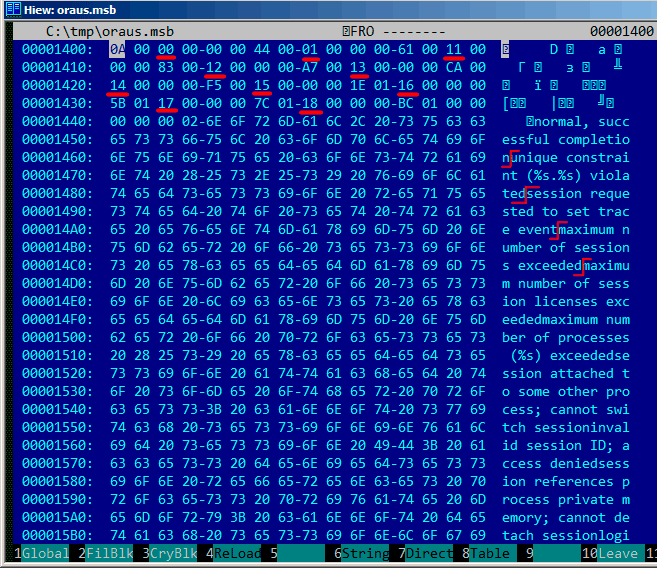
\includegraphics[width=0.6\textwidth]{examples/lines/2.png}
\caption{Practical joke works}
\end{figure}

Oh yes, it works\footnote{Author of this book once did this as a joke for his coworkers with 
the hope that they would stop playing. They didn't.}.

But why are the arguments to the \TT{random()} functions global variables?
That's just because it's possible to change the board size in the game's settings, 
so these values are not hardcoded.
The 10 and 5 values are just defaults.
}\RU{\clearpage
\section{Шутка с игрой Color Lines}
\label{chap:color_lines}

Это очень популярная игра с большим количеством реализаций.
Возьмем одну из них, с названием BallTriX, от 1997, доступную бесплатно на \url{http://go.yurichev.com/17311}
\footnote{Или на \url{http://go.yurichev.com/17365} или \url{http://go.yurichev.com/17366}.}.
Вот как она выглядит:

\begin{figure}[H]
\centering
\includegraphics[width=0.6\textwidth]{examples/lines/1.png}
\caption{Обычный вид игры}
\label{fig:lines_1}
\end{figure}

\clearpage
\myindex{\CStandardLibrary!rand()}
Посмотрим, сможем ли мы найти генератор псевдослучайных чисел и и сделать с ним одну шутку.

\IDA быстро распознает стандартную функцию \TT{\_rand} в 
\TT{balltrix.exe} по адресу \TT{0x00403DA0}.
\IDA также показывает, что она вызывается только из одного места:

\lstinputlisting[style=customasmx86]{examples/lines/random.lst}

Назовем её \q{random}.
Пока не будем концентрироваться на самом коде функции.

Эта функция вызывается из трех мест.

Вот первые два:

\lstinputlisting[style=customasmx86]{examples/lines/1.lst}

Вот третье:

\lstinputlisting[style=customasmx86]{examples/lines/2.lst}

Так что у функции только один аргумент.
10 передается в первых двух случаях и 5 в третьем.

Мы также можем заметить, что размер доски 10*10 и здесь 5 возможных цветов.
Это оно!
Стандартная функция \TT{rand()} возвращает число в пределах \TT{0..0x7FFF} и это неудобно, так что многие программисты пишут свою функцию,
возвращающую случайное число в некоторых заданных пределах.
В нашем случае, предел это $0..n-1$ и $n$ передается как
единственный аргумент в функцию.
Мы можем быстро проверить это в отладчике.

Сделаем так, чтобы третий вызов функции всегда возвращал ноль.
В начале заменим три инструкции (\TT{PUSH/CALL/ADD}) 
на \ac{NOP}s.
Затем добавим инструкцию \INS{XOR EAX, EAX}, для очистки регистра \EAX.

\lstinputlisting[style=customasmx86]{examples/lines/fixed.lst}

Что мы сделали, это заменили вызов функции \TT{random()} 
на код, всегда возвращающий ноль.

\clearpage
Теперь запустим:

\begin{figure}[H]
\centering
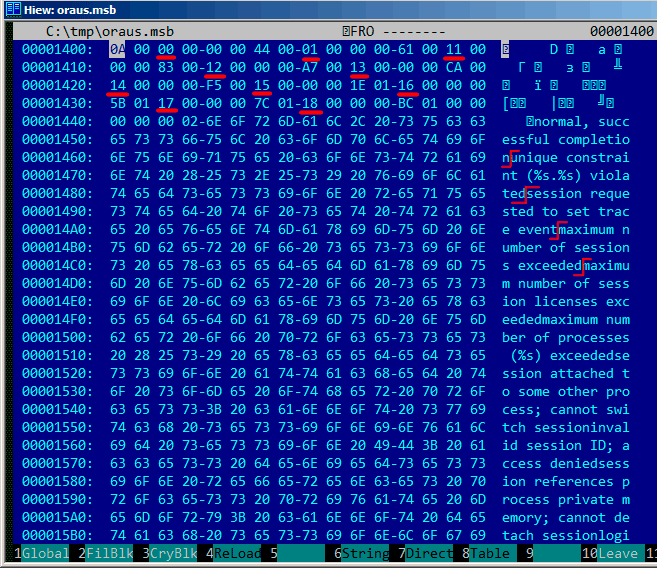
\includegraphics[width=0.6\textwidth]{examples/lines/2.png}
\caption{Шутка сработала}
\end{figure}

О да, это работает\footnote{Автор этой книги однажды сделал это как 
шутку для его сотрудников, в надежде что они перестанут играть. 
Надежды не оправдались.}.

Но почему аргументы функции \TT{random()} это глобальные переменные?
Это просто потому что в настройках игры можно изменять размер доски, так что эти параметры не фиксированы.
10 и 5 это просто значения по умолчанию.
}
\EN{\section{\MinesweeperWinXPExampleChapterName}
\label{minesweeper_winxp}
\myindex{Windows!Windows XP}

For those who are not very good at playing Minesweeper, we could try to reveal the hidden mines in the debugger.

\myindex{\CStandardLibrary!rand()}
\myindex{Windows!PDB}

As we know, Minesweeper places mines randomly, so there has to be some kind of random number generator or
a call to the standard \TT{rand()} C-function.

What is really cool about reversing Microsoft products is that there are \gls{PDB} 
file with symbols (function names, \etc{}).
When we load \TT{winmine.exe} into \IDA, it downloads the 
\gls{PDB} file exactly for this 
executable and shows all names.

So here it is, the only call to \TT{rand()} is this function:

\begin{lstlisting}[style=customasmx86]
.text:01003940 ; __stdcall Rnd(x)
.text:01003940 _Rnd@4          proc near               ; CODE XREF: StartGame()+53
.text:01003940                                         ; StartGame()+61
.text:01003940
.text:01003940 arg_0           = dword ptr  4
.text:01003940
.text:01003940                 call    ds:__imp__rand
.text:01003946                 cdq
.text:01003947                 idiv    [esp+arg_0]
.text:0100394B                 mov     eax, edx
.text:0100394D                 retn    4
.text:0100394D _Rnd@4          endp
\end{lstlisting}

\IDA named it so, and it was the name given to it by Minesweeper's developers.

The function is very simple:

\begin{lstlisting}[style=customc]
int Rnd(int limit)
{
    return rand() % limit;
};
\end{lstlisting}

(There is no \q{limit} name in the \gls{PDB} file; we manually named this argument like this.)

So it returns 
a random value from 0 to a specified limit.

\TT{Rnd()} is called only from one place, 
a function called \TT{StartGame()}, 
and as it seems, this is exactly 
the code which place the mines:

\begin{lstlisting}[style=customasmx86]
.text:010036C7                 push    _xBoxMac
.text:010036CD                 call    _Rnd@4          ; Rnd(x)
.text:010036D2                 push    _yBoxMac
.text:010036D8                 mov     esi, eax
.text:010036DA                 inc     esi
.text:010036DB                 call    _Rnd@4          ; Rnd(x)
.text:010036E0                 inc     eax
.text:010036E1                 mov     ecx, eax
.text:010036E3                 shl     ecx, 5          ; ECX=ECX*32
.text:010036E6                 test    _rgBlk[ecx+esi], 80h
.text:010036EE                 jnz     short loc_10036C7
.text:010036F0                 shl     eax, 5          ; EAX=EAX*32
.text:010036F3                 lea     eax, _rgBlk[eax+esi]
.text:010036FA                 or      byte ptr [eax], 80h
.text:010036FD                 dec     _cBombStart
.text:01003703                 jnz     short loc_10036C7
\end{lstlisting}

Minesweeper allows you to set the board size, so the X (xBoxMac) and Y (yBoxMac) of the board are global variables.
They are passed to \TT{Rnd()} and random 
coordinates are generated.
A mine is placed by the \TT{OR} instruction at \TT{0x010036FA}. 
And if it has been placed before 
(it's possible if the pair of \TT{Rnd()} 
generates a coordinates pair which has been already 
generated), 
then \TT{TEST} and \TT{JNZ} at \TT{0x010036E6} 
jumps to the generation routine again.

\TT{cBombStart} is the global variable containing total number of mines. So this is loop.

The width of the array is 32 
(we can conclude this by looking at the \TT{SHL} instruction, which multiplies one of the coordinates by 32).

The size of the \TT{rgBlk} 
global array can be easily determined by the difference 
between the \TT{rgBlk} 
label in the data segment and the next known one. 
It is 0x360 (864):

\begin{lstlisting}[style=customasmx86]
.data:01005340 _rgBlk          db 360h dup(?)          ; DATA XREF: MainWndProc(x,x,x,x)+574
.data:01005340                                         ; DisplayBlk(x,x)+23
.data:010056A0 _Preferences    dd ?                    ; DATA XREF: FixMenus()+2
...
\end{lstlisting}

$864/32=27$.

So the array size is $27*32$?
It is close to what we know: when we try to set board size to $100*100$ in Minesweeper settings, it fallbacks to a board of size $24*30$.
So this is the maximal board size here.
And the array has a fixed size for any board size.

So let's see all this in \olly.
We will ran Minesweeper, attaching \olly to it and now we can see the memory dump at the address of the \TT{rgBlk} array (\TT{0x01005340})
\footnote{All addresses here are for Minesweeper for Windows XP SP3 English. 
They may differ for other service packs.}.

So we got this memory dump of the array:

\lstinputlisting[style=customasmx86]{examples/minesweeper/1.lst}

\olly, like any other hexadecimal editor, shows 16 bytes per line.
So each 32-byte array row occupies exactly 2 lines here.

This is beginner level (9*9 board).

There is some square 
structure can be seen visually (0x10 bytes).

We will click \q{Run} in \olly to unfreeze the Minesweeper process, then we'll clicked randomly at the Minesweeper window 
and trapped into mine, but now all mines are visible:

\begin{figure}[H]
\centering
\myincludegraphicsSmall{examples/minesweeper/1.png}
\caption{Mines}
\label{fig:minesweeper1}
\end{figure}

By comparing the mine places and the dump, we can conclude that 0x10 stands for border, 0x0F---empty block, 0x8F---mine.

Now we'll add comments and also enclose all 0x8F bytes into square brackets:

\lstinputlisting[style=customasmx86]{examples/minesweeper/2.lst}

Now we'll remove all \IT{border bytes} (0x10) and what's beyond those:

\lstinputlisting[style=customasmx86]{examples/minesweeper/3.lst}

Yes, these are mines, now it can be clearly seen and compared with the screenshot.

\clearpage
What is interesting is that we can modify the array right in \olly.
We can remove all mines by changing all 0x8F bytes by 0x0F, and here is what we'll get in Minesweeper:

\begin{figure}[H]
\centering
\myincludegraphicsSmall{examples/minesweeper/3.png}
\caption{All mines are removed in debugger}
\label{fig:minesweeper3}
\end{figure}

We can also move all of them to the first line: 

\begin{figure}[H]
\centering
\myincludegraphicsSmall{examples/minesweeper/2.png}
\caption{Mines set in debugger}
\label{fig:minesweeper2}
\end{figure}

Well, the debugger is not very convenient for eavesdropping (which is our goal anyway), so we'll write a small utility
to dump the contents of the board:

\lstinputlisting[style=customc]{examples/minesweeper/minesweeper_cheater.c}

Just set the \ac{PID}
\footnote{PID it can be seen in Task Manager 
(enable it in \q{View $\rightarrow$ Select Columns})} 
and the address of the array (\TT{0x01005340} for Windows XP SP3 English) 
and it will dump it
\footnote{The compiled executable is here: 
\href{http://go.yurichev.com/17165}{beginners.re}}.

It attaches itself to a win32 process by \ac{PID} and just reads process memory an the address.

\subsection{Finding grid automatically}

This is kind of nuisance to set address each time when we run our utility.
Also, various Minesweeper versions may have the array on different address.
Knowing the fact that there is always a border (0x10 bytes), we can just find it in memory:

\lstinputlisting[style=customc]{examples/minesweeper/cheater2_fragment.c}

Full source code: \url{https://github.com/dennis714/RE-for-beginners/blob/master/examples/minesweeper/minesweeper_cheater2.c}.

\subsection{\Exercises}

\begin{itemize}

\item 
Why do the \IT{border bytes} (0x10) exist in the array?

What they are for if they are not visible in Minesweeper's interface?
How could it work without them?

\item 
As it turns out, there are more values possible (for open blocks, for flagged by user, \etc{}).
Try to find the meaning of each one.

\item 
Modify my utility so it can remove all mines or set them in a fixed pattern that you want in the Minesweeper
process currently running.

\end{itemize}
}\RU{\section{\MinesweeperWinXPExampleChapterName}
\label{minesweeper_winxp}
\myindex{Windows!Windows XP}

Для тех, кто не очень хорошо играет в Сапёра (Minesweeper), можно попробовать найти все скрытые мины в отладчике.

\myindex{\CStandardLibrary!rand()}
\myindex{Windows!PDB}
Как мы знаем, Сапёр располагает мины случайным образом, так что там должен быть генератор случайных чисел
или вызов стандартной функции Си \TT{rand()}.

Вот что хорошо в реверсинге продуктов от Microsoft, так это то что часто есть \gls{PDB}-файл со всеми
символами (имена функций, \etc{}.).

Когда мы загружаем \TT{winmine.exe} в \IDA, она скачивает 
\gls{PDB} файл именно для этого исполняемого файла и добавляет все имена.

И вот оно, только один вызов \TT{rand()} в этой функции:

\begin{lstlisting}[style=customasmx86]
.text:01003940 ; __stdcall Rnd(x)
.text:01003940 _Rnd@4          proc near               ; CODE XREF: StartGame()+53
.text:01003940                                         ; StartGame()+61
.text:01003940
.text:01003940 arg_0           = dword ptr  4
.text:01003940
.text:01003940                 call    ds:__imp__rand
.text:01003946                 cdq
.text:01003947                 idiv    [esp+arg_0]
.text:0100394B                 mov     eax, edx
.text:0100394D                 retn    4
.text:0100394D _Rnd@4          endp
\end{lstlisting}

Так её назвала \IDA и это было имя данное ей разработчиками Сапёра.

Функция очень простая:

\begin{lstlisting}[style=customc]
int Rnd(int limit)
{
    return rand() % limit;
};
\end{lstlisting}

(В \gls{PDB}-файле не было имени \q{limit}; это мы назвали этот аргумент так, вручную.)

Так что она возвращает случайное число в пределах от нуля до заданного предела.

\TT{Rnd()} вызывается только из одного места, это функция с названием \TT{StartGame()}, 
и как видно, это именно тот код, что расставляет мины:

\begin{lstlisting}[style=customasmx86]
.text:010036C7                 push    _xBoxMac
.text:010036CD                 call    _Rnd@4          ; Rnd(x)
.text:010036D2                 push    _yBoxMac
.text:010036D8                 mov     esi, eax
.text:010036DA                 inc     esi
.text:010036DB                 call    _Rnd@4          ; Rnd(x)
.text:010036E0                 inc     eax
.text:010036E1                 mov     ecx, eax
.text:010036E3                 shl     ecx, 5          ; ECX=ECX*32
.text:010036E6                 test    _rgBlk[ecx+esi], 80h
.text:010036EE                 jnz     short loc_10036C7
.text:010036F0                 shl     eax, 5          ; EAX=EAX*32
.text:010036F3                 lea     eax, _rgBlk[eax+esi]
.text:010036FA                 or      byte ptr [eax], 80h
.text:010036FD                 dec     _cBombStart
.text:01003703                 jnz     short loc_10036C7
\end{lstlisting}

Сапёр позволяет задать размеры доски, так что X (xBoxMac) и Y (yBoxMac) это глобальные переменные.

Они передаются в \TT{Rnd()} и генерируются случайные координаты.
Мина устанавливается инструкцией \TT{OR} на \TT{0x010036FA}. 
И если она уже была установлена до этого 
(это возможно, если пара функций \TT{Rnd()} 
сгенерирует пару, которая уже была сгенерирована), 
тогда \TT{TEST} и \TT{JNZ} на \TT{0x010036E6} 
перейдет на повторную генерацию пары.

\TT{cBombStart} это глобальная переменная, содержащая количество мин. Так что это цикл.

Ширина двухмерного массива это 32 (мы можем это вывести, глядя на инструкцию \TT{SHL}, которая умножает
одну из координат на 32).

Размер глобального массива \TT{rgBlk} 
можно легко узнать по разнице между меткой \TT{rgBlk} 
в сегменте данных и следующей известной меткой. 
Это 0x360 (864):

\begin{lstlisting}[style=customasmx86]
.data:01005340 _rgBlk          db 360h dup(?)          ; DATA XREF: MainWndProc(x,x,x,x)+574
.data:01005340                                         ; DisplayBlk(x,x)+23
.data:010056A0 _Preferences    dd ?                    ; DATA XREF: FixMenus()+2
...
\end{lstlisting}

$864/32=27$.

Так что размер массива $27*32$?
Это близко к тому что мы знаем: если попытаемся установить размер доски в установках Сапёра на $100*100$, то он установит размер $24*30$.
Так что это максимальный размер доски здесь.
И размер массива фиксирован для доски любого размера.

Посмотрим на всё это в \olly.
Запустим Сапёр, присоединим (attach) \olly к нему и увидим содержимое памяти по адресу где массив \TT{rgBlk} (\TT{0x01005340})%

\footnote{Все адреса здесь для Сапёра под Windows XP SP3 English. 
Они могут отличаться для других сервис-паков.}.

Так что у нас выходит такой дамп памяти массива:

\lstinputlisting[style=customasmx86]{examples/minesweeper/1.lst}

\olly, как и любой другой шестнадцатеричный редактор, показывает 16 байт на строку.
Так что каждая 32-байтная строка массива занимает ровно 2 строки.

Это уровень для начинающих (доска 9*9).

Тут еще какая-то квадратная структура, заметная визуально (байты 0x10).

Нажмем \q{Run} в \olly чтобы разморозить процесс Сапёра, потом нажмем в случайное место окна Сапёра, попадаемся на мине, но теперь
видны все мины:

\begin{figure}[H]
\centering
\myincludegraphicsSmall{examples/minesweeper/1.png}
\caption{Мины}
\label{fig:minesweeper1}
\end{figure}

Сравнивая места с минами и дамп, мы можем обнаружить что 0x10 это граница, 0x0F --- пустой блок, 
0x8F --- мина.

Теперь добавим комментариев и также заключим все байты 0x8F в квадратные скобки:%

\lstinputlisting[style=customasmx86]{examples/minesweeper/2.lst}

Теперь уберем все байты связанные с границами (0x10) и всё что за ними:%

\lstinputlisting[style=customasmx86]{examples/minesweeper/3.lst}

Да, это всё мины, теперь это очень хорошо видно, в сравнении со скриншотом.

\clearpage
Вот что интересно, это то что мы можем модифицировать массив прямо в \olly.%

Уберем все мины заменив все байты 0x8F на 0x0F, и вот что получится в Сапёре:

\begin{figure}[H]
\centering
\myincludegraphicsSmall{examples/minesweeper/3.png}
\caption{Все мины убраны в отладчике}
\label{fig:minesweeper3}
\end{figure}

Также уберем их все и добавим их в первом ряду: 

\begin{figure}[H]
\centering
\myincludegraphicsSmall{examples/minesweeper/2.png}
\caption{Мины, установленные в отладчике}
\label{fig:minesweeper2}
\end{figure}

Отладчик не очень удобен для подсматривания (а это была наша изначальная цель), так что напишем маленькую
утилиту для показа содержимого доски:

\lstinputlisting[style=customc]{examples/minesweeper/minesweeper_cheater.c}

Просто установите \ac{PID}
\footnote{PID можно увидеть в Task Manager 
(это можно включить в \q{View $\rightarrow$ Select Columns})} 
и адрес массива (\TT{0x01005340} для Windows XP SP3 English) 
и она покажет его
\footnote{Скомпилированная версия здесь: 
\href{http://go.yurichev.com/17165}{beginners.re}}.

Она подключается к win32-процессу по \ac{PID}-у и просто читает из памяти процесса по этому адресу.

\subsection{Автоматический поиск массива}

Здавать адрес каждый раз при запуске нашей утилиты, это неудобно.
К тому же, разные версии ``Сапёра'' могут иметь этот массив по разным адресам.
Зная, что всегда есть рамка (байты 0x10), массив легко найти в памяти:

\lstinputlisting[style=customc]{examples/minesweeper/cheater2_fragment.c}

Полный исходный код: \url{https://github.com/dennis714/RE-for-beginners/blob/master/examples/minesweeper/minesweeper_cheater2.c}.

\subsection{\Exercises}

\begin{itemize}

\item
Почему байты описывающие границы (0x10) присутствуют вообще?
Зачем они нужны, если они вообще не видимы в интерфейсе Сапёра?
Как можно обойтись без них?

\item
Как выясняется, здесь больше возможных значений (для открытых блоков, для тех на которых игрок установил
флажок, \etc{}.).
	
Попробуйте найти значение каждого.

\item Измените мою утилиту так, чтобы она в запущенном процессе Сапёра убирала все мины, 
или расставляла их в соответствии с каким-то заданным шаблоном.

\end{itemize}
}
\EN{\section{Hacking Windows clock}

Sometimes I did some kind of first April prank for my coworkers.

Let's find, if we could do something with Windows clock?
Can we force to go clock hands backwards?

First of all, when you click on date/time in status bar,\\
a \IT{C:\textbackslash{}WINDOWS\textbackslash{}SYSTEM32\textbackslash{}TIMEDATE.CPL} module gets executed,
which is usual executable PE file.

Let's see, how it draw hands?
When I open the file (from Windows 7) in Resource Hacker, there are clock faces, but with no hands:

\begin{figure}[H]
\centering
\myincludegraphics{examples/timedate/reshack.png}
\caption{Resource Hacker}
\end{figure}

OK, what we know? How to draw a clock hand? All they are started at the middle of circle, ending with its border.
Hence, we must calculate coordinates of a point on circle's border.
From school-level mathematics we may recall that we have to use sine/cosine functions to draw circle, or at least
square root.
There are no such things in \IT{TIMEDATE.CPL}, at least at first glance.
But, thanks to Microsoft debugging PDB files, I can find a function named \IT{CAnalogClock::DrawHand()}, which calls
\IT{Gdiplus::Graphics::DrawLine()} at least twice.

Here is its code:

\lstinputlisting[style=customasmx86]{examples/timedate/1.lst}

\myindex{Windows!Win32!MulDiv()}
We can see that \IT{DrawLine()} arguments are dependent on result of \IT{MulDiv()} function
and a \IT{table[]} table (name is mine),
which has 8-byte elements (look at \INS{LEA}'s second operand).

What is inside of table[]?

\lstinputlisting[style=customasmx86]{examples/timedate/2.lst}

It's referenced only from \IT{DrawHand()} function at has 120 32-bit words or 60 32-bit pairs... wait, 60?
Let's take a closer look at these values.
First of all, I'll zap 6 pairs or 12 32-bit words with zeros, and then I'll put patched \IT{TIMEDATE.CPL}
into \IT{C:\textbackslash{}WINDOWS\textbackslash{}SYSTEM32}.
(You may need to set owner of the *TIMEDATE.CPL* file to your primary user account (instead of \IT{TrustedInstaller}),
and also, boot in safe mode with command prompt so you can copy the file, which is usually locked.)

\begin{figure}[H]
\centering
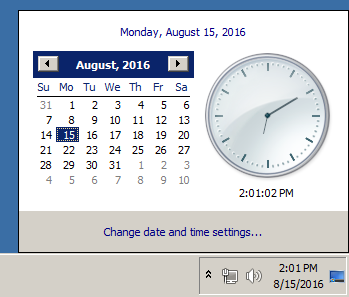
\includegraphics[width=0.5\textwidth]{examples/timedate/6_pairs_zeroed.png}
\caption{Attempt to run}
\end{figure}

Now when any hand is located at 0-5 seconds/minutes, it's invisible! However, opposite (shorter) part of second hand
is visible and moving.
When any hand is outside of this area, hand is visible as usual.

\myindex{Mathematica}
Let's take even closer look at the table in Mathematica.
I have copypasted table from the \IT{TIMEDATE.CPL} to a \IT{tbl} file (480 bytes).
We will take for granted the fact that these are signed values, because half of elements are below zero (0FFFFE0C1h, etc.).
If these values would be unsigned, they would be suspiciously huge.

\begin{lstlisting}[style=custommath]
In[]:= tbl = BinaryReadList["~/.../tbl", "Integer32"]

Out[]= {0, -7999, 836, -7956, 1663, -7825, 2472, -7608, 3253, -7308, 3999, \
-6928, 4702, -6472, 5353, -5945, 5945, -5353, 6472, -4702, 6928, \
-4000, 7308, -3253, 7608, -2472, 7825, -1663, 7956, -836, 8000, 0, \
7956, 836, 7825, 1663, 7608, 2472, 7308, 3253, 6928, 4000, 6472, \
4702, 5945, 5353, 5353, 5945, 4702, 6472, 3999, 6928, 3253, 7308, \
2472, 7608, 1663, 7825, 836, 7956, 0, 7999, -836, 7956, -1663, 7825, \
-2472, 7608, -3253, 7308, -4000, 6928, -4702, 6472, -5353, 5945, \
-5945, 5353, -6472, 4702, -6928, 3999, -7308, 3253, -7608, 2472, \
-7825, 1663, -7956, 836, -7999, 0, -7956, -836, -7825, -1663, -7608, \
-2472, -7308, -3253, -6928, -4000, -6472, -4702, -5945, -5353, -5353, \
-5945, -4702, -6472, -3999, -6928, -3253, -7308, -2472, -7608, -1663, \
-7825, -836, -7956}

In[]:= Length[tbl]
Out[]= 120
\end{lstlisting}

Let's treat two consecutive 32-bit values as pair:

\begin{lstlisting}[style=custommath]
In[]:= pairs = Partition[tbl, 2]
Out[]= {{0, -7999}, {836, -7956}, {1663, -7825}, {2472, -7608}, \
{3253, -7308}, {3999, -6928}, {4702, -6472}, {5353, -5945}, {5945, \
-5353}, {6472, -4702}, {6928, -4000}, {7308, -3253}, {7608, -2472}, \
{7825, -1663}, {7956, -836}, {8000, 0}, {7956, 836}, {7825, 
1663}, {7608, 2472}, {7308, 3253}, {6928, 4000}, {6472, 
4702}, {5945, 5353}, {5353, 5945}, {4702, 6472}, {3999, 
6928}, {3253, 7308}, {2472, 7608}, {1663, 7825}, {836, 7956}, {0, 
7999}, {-836, 7956}, {-1663, 7825}, {-2472, 7608}, {-3253, 
7308}, {-4000, 6928}, {-4702, 6472}, {-5353, 5945}, {-5945, 
5353}, {-6472, 4702}, {-6928, 3999}, {-7308, 3253}, {-7608, 
2472}, {-7825, 1663}, {-7956, 836}, {-7999, 
0}, {-7956, -836}, {-7825, -1663}, {-7608, -2472}, {-7308, -3253}, \
{-6928, -4000}, {-6472, -4702}, {-5945, -5353}, {-5353, -5945}, \
{-4702, -6472}, {-3999, -6928}, {-3253, -7308}, {-2472, -7608}, \
{-1663, -7825}, {-836, -7956}}

In[]:= Length[pairs]
Out[]= 60
\end{lstlisting}

Let's try to treat each pair as X/Y coordinate and draw all 60 pairs, and also first 15 pairs:

\begin{figure}[H]
\centering
\myincludegraphics{examples/timedate/math.png}
\caption{Mathematica}
\end{figure}

Now this is something!
Each pair is just coordinate.
First 15 pairs are coordinates for $\frac{1}{4}$ of circle.

Perhaps, Microsoft developers precalculated all coordinates and put them into table.

Now I can understand why when I zapped 6 pairs, hands were invisible at that area: in fact, hands were drawn,
they just had zero length, because hand started at 0:0 coordinate and ended there.

\subsubsection{The prank (practical joke)}

Given all that, how would we force hands to go counterclockwise?
In fact, this is simple, we need just to rotate the table, so each hand, instead of drawing at place of first second,
would be drawing at place of 59th second.

I made the patcher a long time ago, at the very beginning of 2000s, for Windows 2000.
Hard to believe, it still works for Windows 7, perhaps, the table hasn't been changed since then!

Patcher source code: \url{https://github.com/dennis714/random_notes/blob/master/timedate/time_pt.c}.

Now I can see all hands goes backwards:

\begin{figure}[H]
\centering
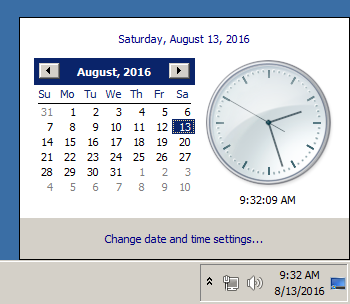
\includegraphics[width=0.5\textwidth]{examples/timedate/counterclockwise.png}
\caption{Now it works}
\end{figure}

Well, there is no animation in this article, but if you look closer, you can see, that hands are in fact shows correct
time, but the whole clock face is rotated vertically, like we see it from the inside of clock.

\subsubsection{Windows 2000 leaked source code}

So I did the patcher and then Windows 2000 source code has been leaked (I can't force you to trust me, though).
Let's take a look on source code if that function and table.\\
The file is \IT{win2k/private/shell/cpls/utc/clock.c}:

\begin{lstlisting}[style=customc]
//
//  Array containing the sine and cosine values for hand positions.
//
POINT rCircleTable[] =
{
    { 0,     -7999},
    { 836,   -7956},
    { 1663,  -7825},
    { 2472,  -7608},
    { 3253,  -7308},
...
    { -4702, -6472},
    { -3999, -6928},
    { -3253, -7308},
    { -2472, -7608},
    { -1663, -7825},
    { -836 , -7956},
};

////////////////////////////////////////////////////////////////////////////
//
//  DrawHand
//
//  Draws the hands of the clock.
//
////////////////////////////////////////////////////////////////////////////

void DrawHand(
    HDC hDC,
    int pos,
    HPEN hPen,
    int scale,
    int patMode,
    PCLOCKSTR np)
{
    LPPOINT lppt;
    int radius;

    MoveTo(hDC, np->clockCenter.x, np->clockCenter.y);
    radius = MulDiv(np->clockRadius, scale, 100);
    lppt = rCircleTable + pos;
    SetROP2(hDC, patMode);
    SelectObject(hDC, hPen);

    LineTo( hDC,
            np->clockCenter.x + MulDiv(lppt->x, radius, 8000),
            np->clockCenter.y + MulDiv(lppt->y, radius, 8000) );
}
\end{lstlisting}

Now it's clear: coordinates has been precalculated as if clock face has height and width of $2 \cdot 8000$,
and then it's rescaled to current clock face radius using \IT{MulDiv()} function.

POINT structure\footnote{\url{https://msdn.microsoft.com/en-us/library/windows/desktop/dd162805(v=vs.85).aspx}}
is a structure of two 32-bit values, first is \IT{x}, second is \IT{y}.

}
\section{\RU{Донглы}\EN{Dongles}}
\label{dongles}

\RU{Автор этих строк иногда делал замену \glslink{dongle}{донглам} или \q{эмуляторы донглов} 
и здесь немного примеров, как это происходит.}
\EN{The author of these lines, occasionally did software copy-protection \gls{dongle} replacements, or \q{dongle emulators} and here
are couple examples of how it's happening.}

\RU{Об одном неописанном здесь случае с Rockey и Z3 вы также можете прочитать здесь}
\EN{About one of the cases about Rocket and Z3 that is not present here, you can read here}:
\url{http://yurichev.com/tmp/SAT_SMT_DRAFT.pdf}.

\EN{\input{examples/dongles/1/main_EN}}\RU{\input{examples/dongles/1/main_RU}}
\EN{\input{examples/dongles/2/main_EN}}\RU{\input{examples/dongles/2/main_RU}}
\EN{\input{examples/dongles/3/main_EN}}\RU{\input{examples/dongles/3/main_RU}}


\EN{\section{
\q{QR9}: Rubik's cube inspired amateur crypto-algorithm}

Sometimes amateur cryptosystems appear to be pretty bizarre.

The author of this book was once asked to reverse engineer an amateur cryptoalgorithm of some data encryption utility, 
the source code for which was lost\footnote{He also got permission from the customer to publish the algorithm's details}.

Here is the listing exported from \IDA for the original encryption utility:

\lstinputlisting[style=customasmx86]{examples/qr9/qr9_original.lst}

All function and label names were given by me during the analysis.

Let's start from the top. Here is a function that takes two file names and password.

\begin{lstlisting}[style=customasmx86]
.text:00541320 ; int __cdecl crypt_file(int Str, char *Filename, int password)
.text:00541320 crypt_file      proc near
.text:00541320
.text:00541320 Str             = dword ptr  4
.text:00541320 Filename        = dword ptr  8
.text:00541320 password        = dword ptr  0Ch
.text:00541320
\end{lstlisting}

Open the file and report if an error occurs:

\begin{lstlisting}[style=customasmx86]
.text:00541320                 mov     eax, [esp+Str]
.text:00541324                 push    ebp
.text:00541325                 push    offset Mode     ; "rb"
.text:0054132A                 push    eax             ; Filename
.text:0054132B                 call    _fopen          ; open file
.text:00541330                 mov     ebp, eax
.text:00541332                 add     esp, 8
.text:00541335                 test    ebp, ebp
.text:00541337                 jnz     short loc_541348
.text:00541339                 push    offset Format   ; "Cannot open input file!\n"
.text:0054133E                 call    _printf
.text:00541343                 add     esp, 4
.text:00541346                 pop     ebp
.text:00541347                 retn
.text:00541348
.text:00541348 loc_541348:
\end{lstlisting}

\myindex{\CStandardLibrary!fseek()}
\myindex{\CStandardLibrary!ftell()}
Get the file size via \TT{fseek()}/\TT{ftell()}:

\lstinputlisting[style=customasmx86]{examples/qr9/1_EN}

This fragment of code calculates the file size aligned on a 64-byte boundary. 
This is because this cryptographic algorithm works with only 64-byte blocks. 
The operation is pretty straightforward: divide the file size by 64, forget about the remainder and add 1, 
then multiply by 64. 
The following code removes the remainder as if the value has already been divided by 64 and adds 64. 
It is almost the same.

\lstinputlisting[style=customasmx86]{examples/qr9/2_EN}

Allocate buffer with aligned size:

\begin{lstlisting}[style=customasmx86]
.text:00541373                 push    esi             ; Size
.text:00541374                 call    _malloc
\end{lstlisting}

\myindex{\CStandardLibrary!calloc()}
Call memset(), e.g., clear the allocated buffer\footnote{malloc() + memset() could 
be replaced by calloc()}.

\lstinputlisting[style=customasmx86]{examples/qr9/3_EN}

Read file via the standard C function \TT{fread()}.

\begin{lstlisting}[style=customasmx86]
.text:00541392                 mov     eax, [esp+38h+Str]
.text:00541396                 push    eax             ; ElementSize
.text:00541397                 push    ebx             ; DstBuf
.text:00541398                 call    _fread          ; read file
.text:0054139D                 push    ebp             ; File
.text:0054139E                 call    _fclose
\end{lstlisting}

Call \TT{crypt()}. This function takes a buffer, buffer size (aligned) and a password string.

\begin{lstlisting}[style=customasmx86]
.text:005413A3                 mov     ecx, [esp+44h+password]
.text:005413A7                 push    ecx             ; password
.text:005413A8                 push    esi             ; aligned size
.text:005413A9                 push    ebx             ; buffer
.text:005413AA                 call    crypt           ; do crypt
\end{lstlisting}

Create the output file. By the way, the developer forgot to check if it has been created correctly! 
The file opening result is being checked, though.

\begin{lstlisting}[style=customasmx86]
.text:005413AF                 mov     edx, [esp+50h+Filename]
.text:005413B3                 add     esp, 40h
.text:005413B6                 push    offset aWb      ; "wb"
.text:005413BB                 push    edx             ; Filename
.text:005413BC                 call    _fopen
.text:005413C1                 mov     edi, eax
\end{lstlisting}

The newly created file handle is in the \EDI register now. Write signature \q{QR9}.

\begin{lstlisting}[style=customasmx86]
.text:005413C3                 push    edi             ; File
.text:005413C4                 push    1               ; Count
.text:005413C6                 push    3               ; Size
.text:005413C8                 push    offset aQr9     ; "QR9"
.text:005413CD                 call    _fwrite         ; write file signature
\end{lstlisting}

Write the actual file size (not aligned):

\begin{lstlisting}[style=customasmx86]
.text:005413D2                 push    edi             ; File
.text:005413D3                 push    1               ; Count
.text:005413D5                 lea     eax, [esp+30h+Str]
.text:005413D9                 push    4               ; Size
.text:005413DB                 push    eax             ; Str
.text:005413DC                 call    _fwrite         ; write original file size
\end{lstlisting}

Write the encrypted buffer:

\begin{lstlisting}[style=customasmx86]
.text:005413E1                 push    edi             ; File
.text:005413E2                 push    1               ; Count
.text:005413E4                 push    esi             ; Size
.text:005413E5                 push    ebx             ; Str
.text:005413E6                 call    _fwrite         ; write encrypted file
\end{lstlisting}

Close the file and free the allocated buffer:

\begin{lstlisting}[style=customasmx86]
.text:005413EB                 push    edi             ; File
.text:005413EC                 call    _fclose
.text:005413F1                 push    ebx             ; Memory
.text:005413F2                 call    _free
.text:005413F7                 add     esp, 40h
.text:005413FA                 pop     edi
.text:005413FB                 pop     esi
.text:005413FC                 pop     ebx
.text:005413FD                 pop     ebp
.text:005413FE                 retn
.text:005413FE crypt_file      endp
\end{lstlisting}

Here is the reconstructed C code:

\begin{lstlisting}[style=customc]
void crypt_file(char *fin, char* fout, char *pw)
{
	FILE *f;
	int flen, flen_aligned;
	BYTE *buf;

	f=fopen(fin, "rb");
	
	if (f==NULL)
	{
		printf ("Cannot open input file!\n");
		return;
	};

	fseek (f, 0, SEEK_END);
	flen=ftell (f);
	fseek (f, 0, SEEK_SET);

	flen_aligned=(flen&0xFFFFFFC0)+0x40;

	buf=(BYTE*)malloc (flen_aligned);
	memset (buf, 0, flen_aligned);

	fread (buf, flen, 1, f);

	fclose (f);

	crypt (buf, flen_aligned, pw);
	
	f=fopen(fout, "wb");

	fwrite ("QR9", 3, 1, f);
	fwrite (&flen, 4, 1, f);
	fwrite (buf, flen_aligned, 1, f);

	fclose (f);

	free (buf);
};
\end{lstlisting}

The decryption procedure is almost the same:

\begin{lstlisting}[style=customasmx86]
.text:00541400 ; int __cdecl decrypt_file(char *Filename, int, void *Src)
.text:00541400 decrypt_file    proc near
.text:00541400
.text:00541400 Filename        = dword ptr  4
.text:00541400 arg_4           = dword ptr  8
.text:00541400 Src             = dword ptr  0Ch
.text:00541400
.text:00541400                 mov     eax, [esp+Filename]
.text:00541404                 push    ebx
.text:00541405                 push    ebp
.text:00541406                 push    esi
.text:00541407                 push    edi
.text:00541408                 push    offset aRb      ; "rb"
.text:0054140D                 push    eax             ; Filename
.text:0054140E                 call    _fopen
.text:00541413                 mov     esi, eax
.text:00541415                 add     esp, 8
.text:00541418                 test    esi, esi
.text:0054141A                 jnz     short loc_54142E
.text:0054141C                 push    offset aCannotOpenIn_0 ; "Cannot open input file!\n"
.text:00541421                 call    _printf
.text:00541426                 add     esp, 4
.text:00541429                 pop     edi
.text:0054142A                 pop     esi
.text:0054142B                 pop     ebp
.text:0054142C                 pop     ebx
.text:0054142D                 retn
.text:0054142E
.text:0054142E loc_54142E:
.text:0054142E                 push    2               ; Origin
.text:00541430                 push    0               ; Offset
.text:00541432                 push    esi             ; File
.text:00541433                 call    _fseek
.text:00541438                 push    esi             ; File
.text:00541439                 call    _ftell
.text:0054143E                 push    0               ; Origin
.text:00541440                 push    0               ; Offset
.text:00541442                 push    esi             ; File
.text:00541443                 mov     ebp, eax
.text:00541445                 call    _fseek
.text:0054144A                 push    ebp             ; Size
.text:0054144B                 call    _malloc
.text:00541450                 push    esi             ; File
.text:00541451                 mov     ebx, eax
.text:00541453                 push    1               ; Count
.text:00541455                 push    ebp             ; ElementSize
.text:00541456                 push    ebx             ; DstBuf
.text:00541457                 call    _fread
.text:0054145C                 push    esi             ; File
.text:0054145D                 call    _fclose
\end{lstlisting}

Check signature (first 3 bytes):

\begin{lstlisting}[style=customasmx86]
.text:00541462                 add     esp, 34h
.text:00541465                 mov     ecx, 3
.text:0054146A                 mov     edi, offset aQr9_0 ; "QR9"
.text:0054146F                 mov     esi, ebx
.text:00541471                 xor     edx, edx
.text:00541473                 repe cmpsb
.text:00541475                 jz      short loc_541489
\end{lstlisting}

Report an error if the signature is absent:

\begin{lstlisting}[style=customasmx86]
.text:00541477                 push    offset aFileIsNotCrypt ; "File is not encrypted!\n"
.text:0054147C                 call    _printf
.text:00541481                 add     esp, 4
.text:00541484                 pop     edi
.text:00541485                 pop     esi
.text:00541486                 pop     ebp
.text:00541487                 pop     ebx
.text:00541488                 retn
.text:00541489
.text:00541489 loc_541489:
\end{lstlisting}

Call \TT{decrypt()}.

\begin{lstlisting}[style=customasmx86]
.text:00541489                 mov     eax, [esp+10h+Src]
.text:0054148D                 mov     edi, [ebx+3]
.text:00541490                 add     ebp, 0FFFFFFF9h
.text:00541493                 lea     esi, [ebx+7]
.text:00541496                 push    eax             ; Src
.text:00541497                 push    ebp             ; int
.text:00541498                 push    esi             ; int
.text:00541499                 call    decrypt
.text:0054149E                 mov     ecx, [esp+1Ch+arg_4]
.text:005414A2                 push    offset aWb_0    ; "wb"
.text:005414A7                 push    ecx             ; Filename
.text:005414A8                 call    _fopen
.text:005414AD                 mov     ebp, eax
.text:005414AF                 push    ebp             ; File
.text:005414B0                 push    1               ; Count
.text:005414B2                 push    edi             ; Size
.text:005414B3                 push    esi             ; Str
.text:005414B4                 call    _fwrite
.text:005414B9                 push    ebp             ; File
.text:005414BA                 call    _fclose
.text:005414BF                 push    ebx             ; Memory
.text:005414C0                 call    _free
.text:005414C5                 add     esp, 2Ch
.text:005414C8                 pop     edi
.text:005414C9                 pop     esi
.text:005414CA                 pop     ebp
.text:005414CB                 pop     ebx
.text:005414CC                 retn
.text:005414CC decrypt_file    endp
\end{lstlisting}

Here is the reconstructed C code:

\begin{lstlisting}[style=customc]
void decrypt_file(char *fin, char* fout, char *pw)
{
	FILE *f;
	int real_flen, flen;
	BYTE *buf;

	f=fopen(fin, "rb");
	
	if (f==NULL)
	{
		printf ("Cannot open input file!\n");
		return;
	};

	fseek (f, 0, SEEK_END);
	flen=ftell (f);
	fseek (f, 0, SEEK_SET);

	buf=(BYTE*)malloc (flen);

	fread (buf, flen, 1, f);

	fclose (f);

	if (memcmp (buf, "QR9", 3)!=0)
	{
		printf ("File is not encrypted!\n");
		return;
	};

	memcpy (&real_flen, buf+3, 4);

	decrypt (buf+(3+4), flen-(3+4), pw);
	
	f=fopen(fout, "wb");

	fwrite (buf+(3+4), real_flen, 1, f);

	fclose (f);

	free (buf);
};
\end{lstlisting}

OK, now let's go deeper.

Function \TT{crypt()}:

\begin{lstlisting}[style=customasmx86]
.text:00541260 crypt           proc near
.text:00541260
.text:00541260 arg_0           = dword ptr  4
.text:00541260 arg_4           = dword ptr  8
.text:00541260 arg_8           = dword ptr  0Ch
.text:00541260
.text:00541260                 push    ebx
.text:00541261                 mov     ebx, [esp+4+arg_0]
.text:00541265                 push    ebp
.text:00541266                 push    esi
.text:00541267                 push    edi
.text:00541268                 xor     ebp, ebp
.text:0054126A
.text:0054126A loc_54126A:
\end{lstlisting}

\myindex{x86!\Instructions!MOVSD}
This fragment of code copies a part of the input buffer to an internal array we later name \q{cube64}.
The size is in the \ECX register. \TT{MOVSD} stands for \IT{move 32-bit dword}, so, 
16 32-bit dwords are exactly 64 bytes.

\begin{lstlisting}[style=customasmx86]
.text:0054126A                 mov     eax, [esp+10h+arg_8]
.text:0054126E                 mov     ecx, 10h
.text:00541273                 mov     esi, ebx   ; EBX is pointer within input buffer
.text:00541275                 mov     edi, offset cube64
.text:0054127A                 push    1
.text:0054127C                 push    eax
.text:0054127D                 rep movsd
\end{lstlisting}

Call \TT{rotate\_all\_with\_password()}:

\begin{lstlisting}[style=customasmx86]
.text:0054127F                 call    rotate_all_with_password
\end{lstlisting}

Copy encrypted contents back from \q{cube64} to buffer:

\begin{lstlisting}[style=customasmx86]
.text:00541284                 mov     eax, [esp+18h+arg_4]
.text:00541288                 mov     edi, ebx
.text:0054128A                 add     ebp, 40h
.text:0054128D                 add     esp, 8
.text:00541290                 mov     ecx, 10h
.text:00541295                 mov     esi, offset cube64
.text:0054129A                 add     ebx, 40h  ; add 64 to input buffer pointer
.text:0054129D                 cmp     ebp, eax  ; EBP = amount of encrypted data.
.text:0054129F                 rep movsd
\end{lstlisting}

If \EBP is not bigger that the size input argument, then continue to the next block.

\begin{lstlisting}[style=customasmx86]
.text:005412A1                 jl      short loc_54126A
.text:005412A3                 pop     edi
.text:005412A4                 pop     esi
.text:005412A5                 pop     ebp
.text:005412A6                 pop     ebx
.text:005412A7                 retn
.text:005412A7 crypt           endp
\end{lstlisting}

Reconstructed \TT{crypt()} function:

\begin{lstlisting}[style=customc]
void crypt (BYTE *buf, int sz, char *pw)
{
	int i=0;
	
	do
	{
		memcpy (cube, buf+i, 8*8);
		rotate_all (pw, 1);
		memcpy (buf+i, cube, 8*8);
		i+=64;
	}
	while (i<sz);
};
\end{lstlisting}

OK, now let's go deeper in function \TT{rotate\_all\_with\_password()}. 
It takes two arguments: password string and a number.

In \TT{crypt()}, the number 1 is used, and in the \TT{decrypt()} function (where \TT{rotate\_all\_with\_password()} function 
is called too), the number is 3.

\begin{lstlisting}[style=customasmx86]
.text:005411B0 rotate_all_with_password proc near
.text:005411B0
.text:005411B0 arg_0           = dword ptr  4
.text:005411B0 arg_4           = dword ptr  8
.text:005411B0
.text:005411B0                 mov     eax, [esp+arg_0]
.text:005411B4                 push    ebp
.text:005411B5                 mov     ebp, eax
\end{lstlisting}

Check the current character in the password. If it is zero, exit:

\begin{lstlisting}[style=customasmx86]
.text:005411B7                 cmp     byte ptr [eax], 0
.text:005411BA                 jz      exit
.text:005411C0                 push    ebx
.text:005411C1                 mov     ebx, [esp+8+arg_4]
.text:005411C5                 push    esi
.text:005411C6                 push    edi
.text:005411C7
.text:005411C7 loop_begin:
\end{lstlisting}

\myindex{\CStandardLibrary!tolower()}
Call \TT{tolower()}, a standard C function.

\begin{lstlisting}[style=customasmx86]
.text:005411C7                 movsx   eax, byte ptr [ebp+0]
.text:005411CB                 push    eax             ; C
.text:005411CC                 call    _tolower
.text:005411D1                 add     esp, 4
\end{lstlisting}

Hmm, if the password has non-Latin character, it is skipped! 
Indeed, when we run the encryption utility and try non-Latin characters in the password, 
they seem to be ignored.

\begin{lstlisting}[style=customasmx86]
.text:005411D4                 cmp     al, 'a'
.text:005411D6                 jl      short next_character_in_password
.text:005411D8                 cmp     al, 'z'
.text:005411DA                 jg      short next_character_in_password
.text:005411DC                 movsx   ecx, al
\end{lstlisting}

Subtract the value of \q{a} (97) from the character.

\begin{lstlisting}[style=customasmx86]
.text:005411DF                 sub     ecx, 'a'  ; 97
\end{lstlisting}

After subtracting, we'll get 0 for \q{a} here, 1 for \q{b}, etc. And 25 for \q{z}.

\begin{lstlisting}[style=customasmx86]
.text:005411E2                 cmp     ecx, 24
.text:005411E5                 jle     short skip_subtracting
.text:005411E7                 sub     ecx, 24
\end{lstlisting}

It seems, \q{y} and \q{z} are exceptional characters too. 
After that fragment of code, \q{y} becomes 0 and \q{z}~---1. 
This implies that the 26 Latin alphabet symbols become values in the range of 0..23, (24 in total).

\begin{lstlisting}[style=customasmx86]
.text:005411EA
.text:005411EA skip_subtracting:                       ; CODE XREF: rotate_all_with_password+35
\end{lstlisting}

This is actually division via multiplication. 
You can read more about it in the \q{\DivisionByMultSectionName} section~(\myref{sec:divisionbymult}).

The code actually divides the password character's value by 3.
% TODO1: add Mathematica calculations
\begin{lstlisting}[style=customasmx86]
.text:005411EA                 mov     eax, 55555556h
.text:005411EF                 imul    ecx
.text:005411F1                 mov     eax, edx
.text:005411F3                 shr     eax, 1Fh
.text:005411F6                 add     edx, eax
.text:005411F8                 mov     eax, ecx
.text:005411FA                 mov     esi, edx
.text:005411FC                 mov     ecx, 3
.text:00541201                 cdq
.text:00541202                 idiv    ecx
\end{lstlisting}

\EDX is the remainder of the division.

\lstinputlisting[style=customasmx86]{examples/qr9/4_EN}

If the remainder is 2, call \TT{rotate3()}. 
\EDI is the second argument of the \TT{rotate\_all\_with\_password()} function.
As we already noted, 1 is for the encryption operations and 3 is for the decryption. 
So, here is a loop. When encrypting, rotate1/2/3 are to be called the same number of times as 
given in the first argument.

\begin{lstlisting}[style=customasmx86]
.text:00541215 call_rotate3:
.text:00541215                 push    esi
.text:00541216                 call    rotate3
.text:0054121B                 add     esp, 4
.text:0054121E                 dec     edi
.text:0054121F                 jnz     short call_rotate3
.text:00541221                 jmp     short next_character_in_password
.text:00541223
.text:00541223 call_rotate2:
.text:00541223                 test    ebx, ebx
.text:00541225                 jle     short next_character_in_password
.text:00541227                 mov     edi, ebx
.text:00541229
.text:00541229 loc_541229:
.text:00541229                 push    esi
.text:0054122A                 call    rotate2
.text:0054122F                 add     esp, 4
.text:00541232                 dec     edi
.text:00541233                 jnz     short loc_541229
.text:00541235                 jmp     short next_character_in_password
.text:00541237
.text:00541237 call_rotate1:
.text:00541237                 test    ebx, ebx
.text:00541239                 jle     short next_character_in_password
.text:0054123B                 mov     edi, ebx
.text:0054123D
.text:0054123D loc_54123D:
.text:0054123D                 push    esi
.text:0054123E                 call    rotate1
.text:00541243                 add     esp, 4
.text:00541246                 dec     edi
.text:00541247                 jnz     short loc_54123D
.text:00541249
\end{lstlisting}

Fetch the next character from the password string.

\begin{lstlisting}[style=customasmx86]
.text:00541249 next_character_in_password:
.text:00541249                 mov     al, [ebp+1]
\end{lstlisting}

\Gls{increment} the character pointer in the password string:

\begin{lstlisting}[style=customasmx86]
.text:0054124C                 inc     ebp
.text:0054124D                 test    al, al
.text:0054124F                 jnz     loop_begin
.text:00541255                 pop     edi
.text:00541256                 pop     esi
.text:00541257                 pop     ebx
.text:00541258
.text:00541258 exit:
.text:00541258                 pop     ebp
.text:00541259                 retn
.text:00541259 rotate_all_with_password endp
\end{lstlisting}

Here is the reconstructed C code:

\begin{lstlisting}[style=customc]
void rotate_all (char *pwd, int v)
{
	char *p=pwd;

	while (*p)
	{
		char c=*p;
		int q;

		c=tolower (c);

		if (c>='a' && c<='z')
		{
			q=c-'a';
			if (q>24)
				q-=24;

			int quotient=q/3;
			int remainder=q % 3;

			switch (remainder)
			{
			case 0: for (int i=0; i<v; i++) rotate1 (quotient); break;
			case 1: for (int i=0; i<v; i++) rotate2 (quotient); break;
			case 2: for (int i=0; i<v; i++) rotate3 (quotient); break;
			};
		};

		p++;
	};
};
\end{lstlisting}

Now let's go deeper and investigate the rotate1/2/3 functions. 
Each function calls another two functions. 
We eventually will name them \TT{set\_bit()} and \TT{get\_bit()}.

Let's start with \TT{get\_bit()}:

\begin{lstlisting}[style=customasmx86]
.text:00541050 get_bit         proc near
.text:00541050
.text:00541050 arg_0           = dword ptr  4
.text:00541050 arg_4           = dword ptr  8
.text:00541050 arg_8           = byte ptr  0Ch
.text:00541050
.text:00541050                 mov     eax, [esp+arg_4]
.text:00541054                 mov     ecx, [esp+arg_0]
.text:00541058                 mov     al, cube64[eax+ecx*8]
.text:0054105F                 mov     cl, [esp+arg_8]
.text:00541063                 shr     al, cl
.text:00541065                 and     al, 1
.text:00541067                 retn
.text:00541067 get_bit         endp
\end{lstlisting}

\dots in other words: calculate an index in 
the cube64 array: \IT{arg\_4 + arg\_0 * 8}.
Then shift a byte from the array by arg\_8 bits right. 
Isolate the lowest bit and return it.

Let's see another function, \TT{set\_bit()}:

\begin{lstlisting}[style=customasmx86]
.text:00541000 set_bit         proc near
.text:00541000
.text:00541000 arg_0           = dword ptr  4
.text:00541000 arg_4           = dword ptr  8
.text:00541000 arg_8           = dword ptr  0Ch
.text:00541000 arg_C           = byte ptr  10h
.text:00541000
.text:00541000                 mov     al, [esp+arg_C]
.text:00541004                 mov     ecx, [esp+arg_8]
.text:00541008                 push    esi
.text:00541009                 mov     esi, [esp+4+arg_0]
.text:0054100D                 test    al, al
.text:0054100F                 mov     eax, [esp+4+arg_4]
.text:00541013                 mov     dl, 1
.text:00541015                 jz      short loc_54102B
\end{lstlisting}

The value in the \TT{DL} is 1 here. It gets shifted left by arg\_8.
For example, if arg\_8 is 4, the value in the \TT{DL} register is to be 
0x10 or 1000b in binary form.

\begin{lstlisting}[style=customasmx86]
.text:00541017                 shl     dl, cl
.text:00541019                 mov     cl, cube64[eax+esi*8]
\end{lstlisting}

Get a bit from array and explicitly set it. % TODO1: rewrite

\begin{lstlisting}[style=customasmx86]
.text:00541020                 or      cl, dl
\end{lstlisting}

Store it back: % TODO1: rewrite

\begin{lstlisting}[style=customasmx86]
.text:00541022                 mov     cube64[eax+esi*8], cl
.text:00541029                 pop     esi
.text:0054102A                 retn
.text:0054102B
.text:0054102B loc_54102B:
.text:0054102B                 shl     dl, cl
\end{lstlisting}

If arg\_C is not zero\dots

\begin{lstlisting}[style=customasmx86]
.text:0054102D                 mov     cl, cube64[eax+esi*8]
\end{lstlisting}

\myindex{x86!\Instructions!NOT}

\dots invert DL. For example, if DL's state after the shift is 0x10 or 0b1000, 
there is 0xEF to be after the \NOT instruction (or 0b11101111b).

\begin{lstlisting}[style=customasmx86]
.text:00541034                 not     dl
\end{lstlisting}

This instruction clears the bit, in other words, it saves all bits in \TT{CL} which are also set in 
\TT{DL} except those in \TT{DL} which are cleared.
This implies that if \TT{DL} is 11101111b in binary form,
all bits are to be saved except the 5th (counting from lowest bit).

\begin{lstlisting}[style=customasmx86]
.text:00541036                 and     cl, dl
\end{lstlisting}

Store it back:

\begin{lstlisting}[style=customasmx86]
.text:00541038                 mov     cube64[eax+esi*8], cl
.text:0054103F                 pop     esi
.text:00541040                 retn
.text:00541040 set_bit         endp
\end{lstlisting}

It is almost the same as \TT{get\_bit()}, except, if arg\_C is zero, the function clears the specific bit in the array, 
or sets it otherwise.

We also know that the array's size is 64. The first two arguments both in the \TT{set\_bit()} and \TT{get\_bit()} functions
could be seen as 2D coordinates. Then the array is to be an 8*8 matrix.

Here is a C representation of what we know up to now:

\begin{lstlisting}[style=customc]
#define IS_SET(flag, bit)       ((flag) & (bit))
#define SET_BIT(var, bit)       ((var) |= (bit))
#define REMOVE_BIT(var, bit)    ((var) &= ~(bit))

static BYTE cube[8][8];

void set_bit (int x, int y, int shift, int bit)
{
	if (bit)
		SET_BIT (cube[x][y], 1<<shift);
	else
		REMOVE_BIT (cube[x][y], 1<<shift);
};

bool get_bit (int x, int y, int shift)
{
	if ((cube[x][y]>>shift)&1==1)
		return 1;
	return 0;
};
\end{lstlisting}

Now let's get back to the rotate1/2/3 functions.

\begin{lstlisting}[style=customasmx86]
.text:00541070 rotate1         proc near
.text:00541070
\end{lstlisting}

Internal array allocation in the local stack, with size of 64 bytes:

\begin{lstlisting}[style=customasmx86]
.text:00541070 internal_array_64= byte ptr -40h
.text:00541070 arg_0           = dword ptr  4
.text:00541070
.text:00541070                 sub     esp, 40h
.text:00541073                 push    ebx
.text:00541074                 push    ebp
.text:00541075                 mov     ebp, [esp+48h+arg_0]
.text:00541079                 push    esi
.text:0054107A                 push    edi
.text:0054107B                 xor     edi, edi        ; EDI is loop1 counter
\end{lstlisting}

\EBX is a pointer to the internal array:

\begin{lstlisting}[style=customasmx86]
.text:0054107D                 lea     ebx, [esp+50h+internal_array_64]
.text:00541081
\end{lstlisting}

Here we have two nested loops:

\lstinputlisting[style=customasmx86]{examples/qr9/5_EN}

\dots we see that both loops' counters are in the range of 0..7. 
Also they are used as the first and second argument for the \TT{get\_bit()} function.
The third argument to \TT{get\_bit()} is the only argument of \TT{rotate1()}. 
The return value from \TT{get\_bit()} is placed in the internal array.

Prepare a pointer to the internal array again:

\lstinputlisting[style=customasmx86]{examples/qr9/6_EN}

\dots this code is placing the contents of the internal array to the cube global array via the \TT{set\_bit()} function, 
\IT{but} in a different order!
Now the counter of the first loop is in the range of 7 to 0, \glslink{decrement}{decrementing} at each iteration!

The C code representation looks like:

\begin{lstlisting}[style=customc]
void rotate1 (int v)
{
	bool tmp[8][8]; // internal array
	int i, j;

	for (i=0; i<8; i++)
		for (j=0; j<8; j++)
			tmp[i][j]=get_bit (i, j, v);

	for (i=0; i<8; i++)
		for (j=0; j<8; j++)
			set_bit (j, 7-i, v, tmp[x][y]);
};
\end{lstlisting}

Not very understandable, but if we take a look at \TT{rotate2()} function:

\lstinputlisting[style=customasmx86]{examples/qr9/7_EN}

It is \IT{almost} the same, except the order of the arguments of the \TT{get\_bit()} and \TT{set\_bit()} is different. 
Let's rewrite it in C-like code:

\begin{lstlisting}[style=customc]
void rotate2 (int v)
{
	bool tmp[8][8]; // internal array
	int i, j;

	for (i=0; i<8; i++)
		for (j=0; j<8; j++)
			tmp[i][j]=get_bit (v, i, j);

	for (i=0; i<8; i++)
		for (j=0; j<8; j++)
			set_bit (v, j, 7-i, tmp[i][j]);
};
\end{lstlisting}

Let's also rewrite the \TT{rotate3()} function:

\begin{lstlisting}[style=customc]
void rotate3 (int v)
{
	bool tmp[8][8];
	int i, j;

	for (i=0; i<8; i++)
		for (j=0; j<8; j++)
			tmp[i][j]=get_bit (i, v, j);

	for (i=0; i<8; i++)
		for (j=0; j<8; j++)
			set_bit (7-j, v, i, tmp[i][j]);
};
\end{lstlisting}

Well, now things are simpler. If we consider cube64 as a 3D cube of size 8*8*8, where each element is a bit, 
\TT{get\_bit()} and \TT{set\_bit()} take just the coordinates of a bit as input.

The rotate1/2/3 functions are in fact rotating all bits in a specific plane. 
These three functions are one for each cube side and the \TT{v} argument sets the plane in the range of 0..7.

Maybe the algorithm's author was thinking of a 8*8*8 Rubik's cube
\footnote{\href{http://go.yurichev.com/17115}{wikipedia}}?!

Yes, indeed.

Let's look closer into the \TT{decrypt()} function, here is its rewritten version:

\begin{lstlisting}[style=customc]
void decrypt (BYTE *buf, int sz, char *pw)
{
	char *p=strdup (pw);
	strrev (p);
	int i=0;

	do
	{
		memcpy (cube, buf+i, 8*8);
		rotate_all (p, 3);
		memcpy (buf+i, cube, 8*8);
		i+=64;
	}
	while (i<sz);
	
	free (p);
};
\end{lstlisting}

It is almost the same as for \TT{crypt()}, \IT{but} the password string is reversed by the
strrev() \footnote{\href{http://go.yurichev.com/17249}{MSDN}}
standard C function and \TT{rotate\_all()} is called with argument 3. 

This implies that in case of decryption, each corresponding rotate1/2/3 call is to be performed thrice.

This is almost as in Rubik'c cube! 
If you want to get back, do the same in reverse order and direction! 
If you want to undo the effect of rotating one place in clockwise direction, 
rotate it once in counter-clockwise direction, or thrice in clockwise direction.

\TT{rotate1()} is apparently for rotating the \q{front} plane. 
\TT{rotate2()} is apparently for rotating the \q{top} plane. 
\TT{rotate3()} is apparently for rotating the \q{left} plane.

Let's get back to the core of the \TT{rotate\_all()} function:

\begin{lstlisting}[style=customc]
q=c-'a';
if (q>24)
	q-=24;

int quotient=q/3; // in range 0..7
int remainder=q % 3;

switch (remainder)
{
    case 0: for (int i=0; i<v; i++) rotate1 (quotient); break; // front
    case 1: for (int i=0; i<v; i++) rotate2 (quotient); break; // top
    case 2: for (int i=0; i<v; i++) rotate3 (quotient); break; // left
};
\end{lstlisting}

Now it is much simpler to understand: each password character defines a side (one of three) and a plane (one of 8). 
3*8 = 24, that is why two the last two characters of the Latin alphabet are remapped to fit an alphabet of exactly 
24 elements.

The algorithm is clearly weak: in case of short passwords you can see
that in the encrypted file there are 
the original bytes of the original file in a binary file editor.

Here is the whole source code reconstructed:

\lstinputlisting[style=customc]{examples/qr9/qr9.cpp}

}\RU{\section{\q{QR9}: Любительская криптосистема, вдохновленная кубиком Рубика}

Любительские криптосистемы иногда встречаются довольно странные.

Однажды автора сих строк попросили разобраться с одним таким любительским криптоалгоритмом встроенным в 
утилиту для шифрования, исходный код которой был утерян\footnote{Он также получил разрешение от 
клиента на публикацию деталей алгоритма}.

Вот листинг этой утилиты для шифрования, полученный при помощи \IDA:

% TODO translate:
\lstinputlisting[style=customasmx86]{examples/qr9/qr9_original.lst}

Все имена функций и меток даны мною в процессе анализа.

Начнем с самого верха. Вот функция, берущая на вход два имени файла и пароль.


\begin{lstlisting}[style=customasmx86]
.text:00541320 ; int __cdecl crypt_file(int Str, char *Filename, int password)
.text:00541320 crypt_file      proc near
.text:00541320
.text:00541320 Str             = dword ptr  4
.text:00541320 Filename        = dword ptr  8
.text:00541320 password        = dword ptr  0Ch
.text:00541320
\end{lstlisting}

Открыть файл и сообщить об ошибке в случае ошибки:

\begin{lstlisting}[style=customasmx86]
.text:00541320                 mov     eax, [esp+Str]
.text:00541324                 push    ebp
.text:00541325                 push    offset Mode     ; "rb"
.text:0054132A                 push    eax             ; Filename
.text:0054132B                 call    _fopen          ; open file
.text:00541330                 mov     ebp, eax
.text:00541332                 add     esp, 8
.text:00541335                 test    ebp, ebp
.text:00541337                 jnz     short loc_541348
.text:00541339                 push    offset Format   ; "Cannot open input file!\n"
.text:0054133E                 call    _printf
.text:00541343                 add     esp, 4
.text:00541346                 pop     ebp
.text:00541347                 retn
.text:00541348
.text:00541348 loc_541348:
\end{lstlisting}

\myindex{\CStandardLibrary!fseek()}
\myindex{\CStandardLibrary!ftell()}
Узнать размер файла используя \TT{fseek()}/\TT{ftell()}:

\lstinputlisting[style=customasmx86]{examples/qr9/1_RU}

Этот фрагмент кода вычисляет длину файла, выровненную по 64-байтной границе.
Это потому что этот алгоритм шифрования работает только с блоками размерами 64 байта.
Работает очень просто: разделить длину файла на 64, забыть об остатке, прибавить 1,
умножить на 64.
Следующий код удаляет остаток от деления, как если бы это значение уже было разделено 
на 64 и добавляет 64. Это почти то же самое.

\lstinputlisting[style=customasmx86]{examples/qr9/2_RU}

Выделить буфер с выровненным размером:

\begin{lstlisting}[style=customasmx86]
.text:00541373                 push    esi             ; Size
.text:00541374                 call    _malloc
\end{lstlisting}

\myindex{\CStandardLibrary!calloc()}
Вызвать memset(), т.е. очистить выделенный буфер\footnote{malloc() + memset() можно было бы 
заменить на calloc()}.

\lstinputlisting[style=customasmx86]{examples/qr9/3_RU}

Чтение файла используя стандартную функцию Си \TT{fread()}.

\begin{lstlisting}[style=customasmx86]
.text:00541392                 mov     eax, [esp+38h+Str]
.text:00541396                 push    eax             ; ElementSize
.text:00541397                 push    ebx             ; DstBuf
.text:00541398                 call    _fread          ; read file
.text:0054139D                 push    ebp             ; File
.text:0054139E                 call    _fclose
\end{lstlisting}

Вызов \TT{crypt()}. Эта функция берет на вход буфер, длину буфера (выровненную) и строку пароля.

\begin{lstlisting}[style=customasmx86]
.text:005413A3                 mov     ecx, [esp+44h+password]
.text:005413A7                 push    ecx             ; password
.text:005413A8                 push    esi             ; aligned size
.text:005413A9                 push    ebx             ; buffer
.text:005413AA                 call    crypt           ; do crypt
\end{lstlisting}

Создать выходной файл. Кстати, разработчик забыл вставить проверку, создался ли файл успешно!
Результат открытия файла, впрочем, проверяется.

\begin{lstlisting}[style=customasmx86]
.text:005413AF                 mov     edx, [esp+50h+Filename]
.text:005413B3                 add     esp, 40h
.text:005413B6                 push    offset aWb      ; "wb"
.text:005413BB                 push    edx             ; Filename
.text:005413BC                 call    _fopen
.text:005413C1                 mov     edi, eax
\end{lstlisting}

Теперь хэндл созданного файла в регистре \EDI. Записываем сигнатуру \q{QR9}.

\begin{lstlisting}[style=customasmx86]
.text:005413C3                 push    edi             ; File
.text:005413C4                 push    1               ; Count
.text:005413C6                 push    3               ; Size
.text:005413C8                 push    offset aQr9     ; "QR9"
.text:005413CD                 call    _fwrite         ; write file signature
\end{lstlisting}

Записываем настоящую длину файла (не выровненную):

\begin{lstlisting}[style=customasmx86]
.text:005413D2                 push    edi             ; File
.text:005413D3                 push    1               ; Count
.text:005413D5                 lea     eax, [esp+30h+Str]
.text:005413D9                 push    4               ; Size
.text:005413DB                 push    eax             ; Str
.text:005413DC                 call    _fwrite         ; write original file size
\end{lstlisting}

Записываем шифрованный буфер:

\begin{lstlisting}[style=customasmx86]
.text:005413E1                 push    edi             ; File
.text:005413E2                 push    1               ; Count
.text:005413E4                 push    esi             ; Size
.text:005413E5                 push    ebx             ; Str
.text:005413E6                 call    _fwrite         ; write encrypted file
\end{lstlisting}

Закрыть файл и освободить выделенный буфер:

\begin{lstlisting}[style=customasmx86]
.text:005413EB                 push    edi             ; File
.text:005413EC                 call    _fclose
.text:005413F1                 push    ebx             ; Memory
.text:005413F2                 call    _free
.text:005413F7                 add     esp, 40h
.text:005413FA                 pop     edi
.text:005413FB                 pop     esi
.text:005413FC                 pop     ebx
.text:005413FD                 pop     ebp
.text:005413FE                 retn
.text:005413FE crypt_file      endp
\end{lstlisting}

Переписанный на Си код:

\begin{lstlisting}[style=customc]
void crypt_file(char *fin, char* fout, char *pw)
{
	FILE *f;
	int flen, flen_aligned;
	BYTE *buf;

	f=fopen(fin, "rb");
	
	if (f==NULL)
	{
		printf ("Cannot open input file!\n");
		return;
	};

	fseek (f, 0, SEEK_END);
	flen=ftell (f);
	fseek (f, 0, SEEK_SET);

	flen_aligned=(flen&0xFFFFFFC0)+0x40;

	buf=(BYTE*)malloc (flen_aligned);
	memset (buf, 0, flen_aligned);

	fread (buf, flen, 1, f);

	fclose (f);

	crypt (buf, flen_aligned, pw);
	
	f=fopen(fout, "wb");

	fwrite ("QR9", 3, 1, f);
	fwrite (&flen, 4, 1, f);
	fwrite (buf, flen_aligned, 1, f);

	fclose (f);

	free (buf);
};
\end{lstlisting}

Процедура дешифрования почти такая же:

\begin{lstlisting}[style=customasmx86]
.text:00541400 ; int __cdecl decrypt_file(char *Filename, int, void *Src)
.text:00541400 decrypt_file    proc near
.text:00541400
.text:00541400 Filename        = dword ptr  4
.text:00541400 arg_4           = dword ptr  8
.text:00541400 Src             = dword ptr  0Ch
.text:00541400
.text:00541400                 mov     eax, [esp+Filename]
.text:00541404                 push    ebx
.text:00541405                 push    ebp
.text:00541406                 push    esi
.text:00541407                 push    edi
.text:00541408                 push    offset aRb      ; "rb"
.text:0054140D                 push    eax             ; Filename
.text:0054140E                 call    _fopen
.text:00541413                 mov     esi, eax
.text:00541415                 add     esp, 8
.text:00541418                 test    esi, esi
.text:0054141A                 jnz     short loc_54142E
.text:0054141C                 push    offset aCannotOpenIn_0 ; "Cannot open input file!\n"
.text:00541421                 call    _printf
.text:00541426                 add     esp, 4
.text:00541429                 pop     edi
.text:0054142A                 pop     esi
.text:0054142B                 pop     ebp
.text:0054142C                 pop     ebx
.text:0054142D                 retn
.text:0054142E
.text:0054142E loc_54142E:
.text:0054142E                 push    2               ; Origin
.text:00541430                 push    0               ; Offset
.text:00541432                 push    esi             ; File
.text:00541433                 call    _fseek
.text:00541438                 push    esi             ; File
.text:00541439                 call    _ftell
.text:0054143E                 push    0               ; Origin
.text:00541440                 push    0               ; Offset
.text:00541442                 push    esi             ; File
.text:00541443                 mov     ebp, eax
.text:00541445                 call    _fseek
.text:0054144A                 push    ebp             ; Size
.text:0054144B                 call    _malloc
.text:00541450                 push    esi             ; File
.text:00541451                 mov     ebx, eax
.text:00541453                 push    1               ; Count
.text:00541455                 push    ebp             ; ElementSize
.text:00541456                 push    ebx             ; DstBuf
.text:00541457                 call    _fread
.text:0054145C                 push    esi             ; File
.text:0054145D                 call    _fclose
\end{lstlisting}

Проверяем сигнатуру (первые 3 байта):

\begin{lstlisting}[style=customasmx86]
.text:00541462                 add     esp, 34h
.text:00541465                 mov     ecx, 3
.text:0054146A                 mov     edi, offset aQr9_0 ; "QR9"
.text:0054146F                 mov     esi, ebx
.text:00541471                 xor     edx, edx
.text:00541473                 repe cmpsb
.text:00541475                 jz      short loc_541489
\end{lstlisting}

Сообщить об ошибке если сигнатура отсутствует:

\begin{lstlisting}[style=customasmx86]
.text:00541477                 push    offset aFileIsNotCrypt ; "File is not encrypted!\n"
.text:0054147C                 call    _printf
.text:00541481                 add     esp, 4
.text:00541484                 pop     edi
.text:00541485                 pop     esi
.text:00541486                 pop     ebp
.text:00541487                 pop     ebx
.text:00541488                 retn
.text:00541489
.text:00541489 loc_541489:
\end{lstlisting}

Вызвать \TT{decrypt()}.

\begin{lstlisting}[style=customasmx86]
.text:00541489                 mov     eax, [esp+10h+Src]
.text:0054148D                 mov     edi, [ebx+3]
.text:00541490                 add     ebp, 0FFFFFFF9h
.text:00541493                 lea     esi, [ebx+7]
.text:00541496                 push    eax             ; Src
.text:00541497                 push    ebp             ; int
.text:00541498                 push    esi             ; int
.text:00541499                 call    decrypt
.text:0054149E                 mov     ecx, [esp+1Ch+arg_4]
.text:005414A2                 push    offset aWb_0    ; "wb"
.text:005414A7                 push    ecx             ; Filename
.text:005414A8                 call    _fopen
.text:005414AD                 mov     ebp, eax
.text:005414AF                 push    ebp             ; File
.text:005414B0                 push    1               ; Count
.text:005414B2                 push    edi             ; Size
.text:005414B3                 push    esi             ; Str
.text:005414B4                 call    _fwrite
.text:005414B9                 push    ebp             ; File
.text:005414BA                 call    _fclose
.text:005414BF                 push    ebx             ; Memory
.text:005414C0                 call    _free
.text:005414C5                 add     esp, 2Ch
.text:005414C8                 pop     edi
.text:005414C9                 pop     esi
.text:005414CA                 pop     ebp
.text:005414CB                 pop     ebx
.text:005414CC                 retn
.text:005414CC decrypt_file    endp
\end{lstlisting}

Переписанный на Си код:

\begin{lstlisting}[style=customc]
void decrypt_file(char *fin, char* fout, char *pw)
{
	FILE *f;
	int real_flen, flen;
	BYTE *buf;

	f=fopen(fin, "rb");
	
	if (f==NULL)
	{
		printf ("Cannot open input file!\n");
		return;
	};

	fseek (f, 0, SEEK_END);
	flen=ftell (f);
	fseek (f, 0, SEEK_SET);

	buf=(BYTE*)malloc (flen);

	fread (buf, flen, 1, f);

	fclose (f);

	if (memcmp (buf, "QR9", 3)!=0)
	{
		printf ("File is not encrypted!\n");
		return;
	};

	memcpy (&real_flen, buf+3, 4);

	decrypt (buf+(3+4), flen-(3+4), pw);
	
	f=fopen(fout, "wb");

	fwrite (buf+(3+4), real_flen, 1, f);

	fclose (f);

	free (buf);
};
\end{lstlisting}

OK, посмотрим глубже.

Функция \TT{crypt()}:

\begin{lstlisting}[style=customasmx86]
.text:00541260 crypt           proc near
.text:00541260
.text:00541260 arg_0           = dword ptr  4
.text:00541260 arg_4           = dword ptr  8
.text:00541260 arg_8           = dword ptr  0Ch
.text:00541260
.text:00541260                 push    ebx
.text:00541261                 mov     ebx, [esp+4+arg_0]
.text:00541265                 push    ebp
.text:00541266                 push    esi
.text:00541267                 push    edi
.text:00541268                 xor     ebp, ebp
.text:0054126A
.text:0054126A loc_54126A:
\end{lstlisting}

\myindex{x86!\Instructions!MOVSD}
Этот фрагмент кода копирует часть входного буфера во внутренний буфер, который мы позже назовем \q{cube64}.%

Длина в регистре \ECX. \TT{MOVSD} означает \IT{скопировать 32-битное слово}, так что, 16 32-битных слов
это как раз 64 байта.

\begin{lstlisting}[style=customasmx86]
.text:0054126A                 mov     eax, [esp+10h+arg_8]
.text:0054126E                 mov     ecx, 10h
.text:00541273                 mov     esi, ebx   ; EBX is pointer within input buffer
.text:00541275                 mov     edi, offset cube64
.text:0054127A                 push    1
.text:0054127C                 push    eax
.text:0054127D                 rep movsd
\end{lstlisting}

Вызвать \TT{rotate\_all\_with\_password()}:

\begin{lstlisting}[style=customasmx86]
.text:0054127F                 call    rotate_all_with_password
\end{lstlisting}

Скопировать зашифрованное содержимое из \q{cube64} назад в буфер:

\begin{lstlisting}[style=customasmx86]
.text:00541284                 mov     eax, [esp+18h+arg_4]
.text:00541288                 mov     edi, ebx
.text:0054128A                 add     ebp, 40h
.text:0054128D                 add     esp, 8
.text:00541290                 mov     ecx, 10h
.text:00541295                 mov     esi, offset cube64
.text:0054129A                 add     ebx, 40h  ; add 64 to input buffer pointer
.text:0054129D                 cmp     ebp, eax  ; EBP = amount of encrypted data.
.text:0054129F                 rep movsd
\end{lstlisting}

Если \EBP не больше чем длина во входном аргументе, тогда переходим к следующему блоку.

\begin{lstlisting}[style=customasmx86]
.text:005412A1                 jl      short loc_54126A
.text:005412A3                 pop     edi
.text:005412A4                 pop     esi
.text:005412A5                 pop     ebp
.text:005412A6                 pop     ebx
.text:005412A7                 retn
.text:005412A7 crypt           endp
\end{lstlisting}

Реконструированная функция \TT{crypt()}:

\begin{lstlisting}[style=customc]
void crypt (BYTE *buf, int sz, char *pw)
{
	int i=0;
	
	do
	{
		memcpy (cube, buf+i, 8*8);
		rotate_all (pw, 1);
		memcpy (buf+i, cube, 8*8);
		i+=64;
	}
	while (i<sz);
};
\end{lstlisting}

OK, углубимся в функцию \TT{rotate\_all\_with\_password()}. Она берет на вход два аргумента: 
строку пароля и число.
В функции \TT{crypt()}, число 1 используется и в \TT{decrypt()} \\
(где \TT{rotate\_all\_with\_password()} функция вызывается также), число 3.

\begin{lstlisting}[style=customasmx86]
.text:005411B0 rotate_all_with_password proc near
.text:005411B0
.text:005411B0 arg_0           = dword ptr  4
.text:005411B0 arg_4           = dword ptr  8
.text:005411B0
.text:005411B0                 mov     eax, [esp+arg_0]
.text:005411B4                 push    ebp
.text:005411B5                 mov     ebp, eax
\end{lstlisting}

Проверяем символы в пароле. Если это ноль, выходим:

\begin{lstlisting}[style=customasmx86]
.text:005411B7                 cmp     byte ptr [eax], 0
.text:005411BA                 jz      exit
.text:005411C0                 push    ebx
.text:005411C1                 mov     ebx, [esp+8+arg_4]
.text:005411C5                 push    esi
.text:005411C6                 push    edi
.text:005411C7
.text:005411C7 loop_begin:
\end{lstlisting}

\myindex{\CStandardLibrary!tolower()}
Вызываем \TT{tolower()}, стандартную функцию Си.

\begin{lstlisting}[style=customasmx86]
.text:005411C7                 movsx   eax, byte ptr [ebp+0]
.text:005411CB                 push    eax             ; C
.text:005411CC                 call    _tolower
.text:005411D1                 add     esp, 4
\end{lstlisting}

Хмм, если пароль содержит символ не из латинского алфавита, он пропускается!
Действительно, если мы запускаем утилиту для шифрования используя символы не латинского алфавита, 
похоже, они просто игнорируются.

\begin{lstlisting}[style=customasmx86]
.text:005411D4                 cmp     al, 'a'
.text:005411D6                 jl      short next_character_in_password
.text:005411D8                 cmp     al, 'z'
.text:005411DA                 jg      short next_character_in_password
.text:005411DC                 movsx   ecx, al
\end{lstlisting}

Отнимем значение \q{a} (97) от символа.

\begin{lstlisting}[style=customasmx86]
.text:005411DF                 sub     ecx, 'a'  ; 97
\end{lstlisting}

После вычитания, тут будет 0 для \q{a}, 1 для \q{b}, и так далее. И 25 для \q{z}.

\begin{lstlisting}[style=customasmx86]
.text:005411E2                 cmp     ecx, 24
.text:005411E5                 jle     short skip_subtracting
.text:005411E7                 sub     ecx, 24
\end{lstlisting}

Похоже, символы \q{y} и \q{z} также исключительные.
После этого фрагмента кода, \q{y} становится 0, а \q{z} ~--- 1.
Это значит, что 26 латинских букв становятся значениями в интервале 0..23, (всего 24).

\begin{lstlisting}[style=customasmx86]
.text:005411EA
.text:005411EA skip_subtracting:                       ; CODE XREF: rotate_all_with_password+35
\end{lstlisting}

Это, на самом деле, деление через умножение.
Читайте об этом больше в секции \q{\DivisionByMultSectionName}~(\myref{sec:divisionbymult}).

Это код, на самом деле, делит значение символа пароля на 3.

% TODO1: add Mathematica calculations
\begin{lstlisting}[style=customasmx86]
.text:005411EA                 mov     eax, 55555556h
.text:005411EF                 imul    ecx
.text:005411F1                 mov     eax, edx
.text:005411F3                 shr     eax, 1Fh
.text:005411F6                 add     edx, eax
.text:005411F8                 mov     eax, ecx
.text:005411FA                 mov     esi, edx
.text:005411FC                 mov     ecx, 3
.text:00541201                 cdq
.text:00541202                 idiv    ecx
\end{lstlisting}

\EDX --- остаток от деления.

\lstinputlisting[style=customasmx86]{examples/qr9/4_RU}

Если остаток 2, вызываем \TT{rotate3()}. 
\EDX это второй аргумент функции \TT{rotate\_all\_with\_password()}. 
Как мы уже заметили, 1 это для шифрования, 3 для дешифрования.
Так что здесь цикл, функции rotate1/2/3 будут вызываться столько же раз, сколько значение переменной
в первом аргументе.

\begin{lstlisting}[style=customasmx86]
.text:00541215 call_rotate3:
.text:00541215                 push    esi
.text:00541216                 call    rotate3
.text:0054121B                 add     esp, 4
.text:0054121E                 dec     edi
.text:0054121F                 jnz     short call_rotate3
.text:00541221                 jmp     short next_character_in_password
.text:00541223
.text:00541223 call_rotate2:
.text:00541223                 test    ebx, ebx
.text:00541225                 jle     short next_character_in_password
.text:00541227                 mov     edi, ebx
.text:00541229
.text:00541229 loc_541229:
.text:00541229                 push    esi
.text:0054122A                 call    rotate2
.text:0054122F                 add     esp, 4
.text:00541232                 dec     edi
.text:00541233                 jnz     short loc_541229
.text:00541235                 jmp     short next_character_in_password
.text:00541237
.text:00541237 call_rotate1:
.text:00541237                 test    ebx, ebx
.text:00541239                 jle     short next_character_in_password
.text:0054123B                 mov     edi, ebx
.text:0054123D
.text:0054123D loc_54123D:
.text:0054123D                 push    esi
.text:0054123E                 call    rotate1
.text:00541243                 add     esp, 4
.text:00541246                 dec     edi
.text:00541247                 jnz     short loc_54123D
.text:00541249
\end{lstlisting}

Достать следующий символ из строки пароля.

\begin{lstlisting}[style=customasmx86]
.text:00541249 next_character_in_password:
.text:00541249                 mov     al, [ebp+1]
\end{lstlisting}

\glslink{increment}{Инкремент} указателя на символ в строке пароля:

\begin{lstlisting}[style=customasmx86]
.text:0054124C                 inc     ebp
.text:0054124D                 test    al, al
.text:0054124F                 jnz     loop_begin
.text:00541255                 pop     edi
.text:00541256                 pop     esi
.text:00541257                 pop     ebx
.text:00541258
.text:00541258 exit:
.text:00541258                 pop     ebp
.text:00541259                 retn
.text:00541259 rotate_all_with_password endp
\end{lstlisting}

Реконструированный код на Си:

\begin{lstlisting}[style=customc]
void rotate_all (char *pwd, int v)
{
	char *p=pwd;

	while (*p)
	{
		char c=*p;
		int q;

		c=tolower (c);

		if (c>='a' && c<='z')
		{
			q=c-'a';
			if (q>24)
				q-=24;

			int quotient=q/3;
			int remainder=q % 3;

			switch (remainder)
			{
			case 0: for (int i=0; i<v; i++) rotate1 (quotient); break;
			case 1: for (int i=0; i<v; i++) rotate2 (quotient); break;
			case 2: for (int i=0; i<v; i++) rotate3 (quotient); break;
			};
		};

		p++;
	};
};
\end{lstlisting}

Углубимся еще дальше и исследуем функции rotate1/2/3.
Каждая функция вызывает еще две.
В итоге мы назовем их \TT{set\_bit()} и \TT{get\_bit()}.

Начнем с \TT{get\_bit()}:

\begin{lstlisting}[style=customasmx86]
.text:00541050 get_bit         proc near
.text:00541050
.text:00541050 arg_0           = dword ptr  4
.text:00541050 arg_4           = dword ptr  8
.text:00541050 arg_8           = byte ptr  0Ch
.text:00541050
.text:00541050                 mov     eax, [esp+arg_4]
.text:00541054                 mov     ecx, [esp+arg_0]
.text:00541058                 mov     al, cube64[eax+ecx*8]
.text:0054105F                 mov     cl, [esp+arg_8]
.text:00541063                 shr     al, cl
.text:00541065                 and     al, 1
.text:00541067                 retn
.text:00541067 get_bit         endp
\end{lstlisting}

\dots иными словами: подсчитать индекс в массиве cube64: \IT{arg\_4 + arg\_0 * 8}.
Затем сдвинуть байт из массива вправо на количество бит заданных в arg\_8. 
Изолировать самый младший бит и вернуть его

Посмотрим другую функцию, \TT{set\_bit()}:

\begin{lstlisting}[style=customasmx86]
.text:00541000 set_bit         proc near
.text:00541000
.text:00541000 arg_0           = dword ptr  4
.text:00541000 arg_4           = dword ptr  8
.text:00541000 arg_8           = dword ptr  0Ch
.text:00541000 arg_C           = byte ptr  10h
.text:00541000
.text:00541000                 mov     al, [esp+arg_C]
.text:00541004                 mov     ecx, [esp+arg_8]
.text:00541008                 push    esi
.text:00541009                 mov     esi, [esp+4+arg_0]
.text:0054100D                 test    al, al
.text:0054100F                 mov     eax, [esp+4+arg_4]
.text:00541013                 mov     dl, 1
.text:00541015                 jz      short loc_54102B
\end{lstlisting}

\TT{DL} тут равно 1. Сдвигаем эту единицу на количество, указанное в arg\_8. Например, если в arg\_8 число 4,
тогда значение в \TT{DL} станет 0x10 или 1000b в двоичной системе счисления.

\begin{lstlisting}[style=customasmx86]
.text:00541017                 shl     dl, cl
.text:00541019                 mov     cl, cube64[eax+esi*8]
\end{lstlisting}

Вытащить бит из массива и явно выставить его. % TODO1: rewrite

\begin{lstlisting}[style=customasmx86]
.text:00541020                 or      cl, dl
\end{lstlisting}

Сохранить его назад: % TODO1: rewrite

\begin{lstlisting}[style=customasmx86]
.text:00541022                 mov     cube64[eax+esi*8], cl
.text:00541029                 pop     esi
.text:0054102A                 retn
.text:0054102B
.text:0054102B loc_54102B:
.text:0054102B                 shl     dl, cl
\end{lstlisting}

Если arg\_C не ноль\dots

\begin{lstlisting}[style=customasmx86]
.text:0054102D                 mov     cl, cube64[eax+esi*8]
\end{lstlisting}

\myindex{x86!\Instructions!NOT}
\dots инвертировать DL. Например, если состояние DL после сдвига 0x10 или 1000b в двоичной системе,
здесь будет 0xEF после инструкции \NOT или 11101111b в двоичной системе.

\begin{lstlisting}[style=customasmx86]
.text:00541034                 not     dl
\end{lstlisting}

Эта инструкция сбрасывает бит, иными словами, она сохраняет все биты в \TT{CL} которые также
выставлены в \TT{DL} кроме тех в \TT{DL}, что были сброшены. Это значит, что если в \TT{DL}, например,
11101111b в двоичной системе, все биты будут сохранены кроме пятого (считая с младшего бита).

\begin{lstlisting}[style=customasmx86]
.text:00541036                 and     cl, dl
\end{lstlisting}

Сохранить его назад

\begin{lstlisting}[style=customasmx86]
.text:00541038                 mov     cube64[eax+esi*8], cl
.text:0054103F                 pop     esi
.text:00541040                 retn
.text:00541040 set_bit         endp
\end{lstlisting}

Это почти то же самое что и \TT{get\_bit()}, кроме того, что если arg\_C ноль, тогда функция сбрасывает
указанный бит в массиве, либо же, в противном случае, выставляет его в 1.

Мы также знаем что размер массива 64. Первые два аргумента и у \TT{set\_bit()} и у \TT{get\_bit()}
могут быть представлены как двумерные координаты. Таким образом, массив ~--- это матрица 8*8.

Представление на Си всего того, что мы уже знаем:

\begin{lstlisting}[style=customc]
#define IS_SET(flag, bit)       ((flag) & (bit))
#define SET_BIT(var, bit)       ((var) |= (bit))
#define REMOVE_BIT(var, bit)    ((var) &= ~(bit))

static BYTE cube[8][8];

void set_bit (int x, int y, int shift, int bit)
{
	if (bit)
		SET_BIT (cube[x][y], 1<<shift);
	else
		REMOVE_BIT (cube[x][y], 1<<shift);
};

bool get_bit (int x, int y, int shift)
{
	if ((cube[x][y]>>shift)&1==1)
		return 1;
	return 0;
};
\end{lstlisting}

Теперь вернемся к функциям rotate1/2/3.

\begin{lstlisting}[style=customasmx86]
.text:00541070 rotate1         proc near
.text:00541070
\end{lstlisting}

Выделение внутреннего массива размером 64 байта в локальном стеке:

\begin{lstlisting}[style=customasmx86]
.text:00541070 internal_array_64= byte ptr -40h
.text:00541070 arg_0           = dword ptr  4
.text:00541070
.text:00541070                 sub     esp, 40h
.text:00541073                 push    ebx
.text:00541074                 push    ebp
.text:00541075                 mov     ebp, [esp+48h+arg_0]
.text:00541079                 push    esi
.text:0054107A                 push    edi
.text:0054107B                 xor     edi, edi        ; EDI is loop1 counter
\end{lstlisting}

\EBX указывает на внутренний массив

\begin{lstlisting}[style=customasmx86]
.text:0054107D                 lea     ebx, [esp+50h+internal_array_64]
.text:00541081
\end{lstlisting}

Здесь два вложенных цикла:

\lstinputlisting[style=customasmx86]{examples/qr9/5_RU}

Мы видим, что оба счетчика циклов в интервале 0..7. 
Также, они используются как первый и второй аргумент \TT{get\_bit()}.
Третий аргумент \TT{get\_bit()} это единственный аргумент \TT{rotate1()}. 
То что возвращает \TT{get\_bit()} будет сохранено во внутреннем массиве.

Снова приготовить указатель на внутренний массив:

\lstinputlisting[style=customasmx86]{examples/qr9/6_RU}

\dots этот код помещает содержимое из внутреннего массива в глобальный массив cube используя функцию 
\TT{set\_bit()}, \IT{но}, в обратном порядке!
Теперь счетчик первого цикла в интервале 7 до 0, уменьшается на 1 на каждой итерации!

Представление кода на Си выглядит так:

\begin{lstlisting}[style=customc]
void rotate1 (int v)
{
	bool tmp[8][8]; // internal array
	int i, j;

	for (i=0; i<8; i++)
		for (j=0; j<8; j++)
			tmp[i][j]=get_bit (i, j, v);

	for (i=0; i<8; i++)
		for (j=0; j<8; j++)
			set_bit (j, 7-i, v, tmp[x][y]);
};
\end{lstlisting}

Не очень понятно, но если мы посмотрим в функцию \TT{rotate2()}:

\lstinputlisting[style=customasmx86]{examples/qr9/7_RU}

\IT{Почти} то же самое, за исключением иного порядка аргументов в \TT{get\_bit()} и \TT{set\_bit()}.
Перепишем это на Си-подобный код:

\begin{lstlisting}[style=customc]
void rotate2 (int v)
{
	bool tmp[8][8]; // internal array
	int i, j;

	for (i=0; i<8; i++)
		for (j=0; j<8; j++)
			tmp[i][j]=get_bit (v, i, j);

	for (i=0; i<8; i++)
		for (j=0; j<8; j++)
			set_bit (v, j, 7-i, tmp[i][j]);
};
\end{lstlisting}

Перепишем так же функцию \TT{rotate3()}:

\begin{lstlisting}[style=customasmx86]
void rotate3 (int v)
{
	bool tmp[8][8];
	int i, j;

	for (i=0; i<8; i++)
		for (j=0; j<8; j++)
			tmp[i][j]=get_bit (i, v, j);

	for (i=0; i<8; i++)
		for (j=0; j<8; j++)
			set_bit (7-j, v, i, tmp[i][j]);
};
\end{lstlisting}

Теперь всё проще. Если мы представим cube64 как трехмерный куб 8*8*8, где каждый элемент это бит,
то \TT{get\_bit()} и \TT{set\_bit()} просто берут на вход координаты бита.

Функции rotate1/2/3 просто поворачивают все биты на определенной плоскости.
Три функции, каждая на каждую сторону куба и аргумент \TT{v} выставляет плоскость в интервале 0..7

Может быть, автор алгоритма думал о кубике Рубика 8*8*8

\footnote{\href{http://go.yurichev.com/17115}{wikipedia}}?!

Да, действительно.

Рассмотрим функцию \TT{decrypt()}, вот её переписанная версия:%

\begin{lstlisting}[style=customc]
void decrypt (BYTE *buf, int sz, char *pw)
{
	char *p=strdup (pw);
	strrev (p);
	int i=0;

	do
	{
		memcpy (cube, buf+i, 8*8);
		rotate_all (p, 3);
		memcpy (buf+i, cube, 8*8);
		i+=64;
	}
	while (i<sz);
	
	free (p);
};
\end{lstlisting}

Почти то же самое что и crypt(), \IT{но} строка пароля разворачивается стандартной функцией Си
strrev() \footnote{\href{http://go.yurichev.com/17249}{MSDN}}
и \TT{rotate\_all()} вызывается с аргументом 3.

Это значит, что, в случае дешифровки, rotate1/2/3 будут вызываться трижды.

Это почти кубик Рубика!
Если вы хотите вернуть его состояние назад, делайте то же самое в обратном порядке и направлении!
Чтобы вернуть эффект от поворота плоскости по часовой стрелке, нужно повернуть её же против 
часовой стрелки, либо же трижды по часовой стрелке.

\TT{rotate1()}, вероятно, поворот \q{лицевой} плоскости. 
\TT{rotate2()}, вероятно, поворот \q{верхней} плоскости.
\TT{rotate3()}, вероятно, поворот \q{левой} плоскости.

Вернемся к ядру функции \TT{rotate\_all()}

\begin{lstlisting}[style=customc]
q=c-'a';
if (q>24)
	q-=24;

int quotient=q/3; // in range 0..7
int remainder=q % 3;

switch (remainder)
{
    case 0: for (int i=0; i<v; i++) rotate1 (quotient); break; // front
    case 1: for (int i=0; i<v; i++) rotate2 (quotient); break; // top
    case 2: for (int i=0; i<v; i++) rotate3 (quotient); break; // left
};
\end{lstlisting}

Так понять проще: каждый символ пароля определяет сторону (одну из трех) и плоскость (одну из восьми).
3*8 = 24, вот почему два последних символа латинского алфавита переопределяются так чтобы алфавит состоял
из 24-х элементов.

Алгоритм очевидно слаб: в случае коротких паролей, в бинарном редакторе файлов можно будет увидеть, 
что в зашифрованных файлах остались незашифрованные символы.

Весь исходный код в реконструированном виде:

\lstinputlisting[style=customc]{examples/qr9/qr9.cpp}

}
\EN{% TODO: OpenSSL tool, URLs, etc
\section{Encrypted database case \#1}
\label{encrypted_DB1}

(This part has been first appeared in my blog at 26-Aug-2015.
Some discussion: \url{https://news.ycombinator.com/item?id=10128684}.)

\subsection{Base64 and entropy}

\myindex{XML}
I've got the XML file containing some encrypted data.
Perhaps, it's related to some orders and/or customers information.

\begin{lstlisting}
<?xml version = "1.0" encoding = "UTF-8"?>
<Orders>
	<Order>
		<OrderID>1</OrderID>
		<Data>yjmxhXUbhB/5MV45chPsXZWAJwIh1S0aD9lFn3XuJMSxJ3/E+UE3hsnH</Data>
	</Order>
	<Order>
		<OrderID>2</OrderID>
		<Data>0KGe/wnypFBjsy+U0C2P9fC5nDZP3XDZLMPCRaiBw9OjIk6Tu5U=</Data>
	</Order>
	<Order>
		<OrderID>3</OrderID>
		<Data>mqkXfdzvQKvEArdzh+zD9oETVGBFvcTBLs2ph1b5bYddExzp</Data>
	</Order>
	<Order>
		<OrderID>4</OrderID>
		<Data>FCx6JhIDqnESyT3HAepyE1BJ3cJd7wCk+APCRUeuNtZdpCvQ2MR/7kLXtfUHuA==</Data>
	</Order>
...
\end{lstlisting}

The file is available \href{https://raw.githubusercontent.com/dennis714/yurichev.com/master/blog/encrypted_DB_case_1/encrypted.xml}{here}.

\myindex{base64}
This is clearly base64-encoded data, because all strings consisting of Latin characters, digits,
plus (+) and slash (/) symbols.
There can be 1 or 2 padding symbols (=), but they are never occurred in the middle of string.
Keeping in mind these base64 properties, it's very easy to recognize them.

Let's decode them and calculate entropies (\myref{entropy}) of these blocks in Wolfram Mathematica:

\begin{lstlisting}
In[]:= ListOfBase64Strings = 
  Map[First[#[[3]]] &, Cases[Import["encrypted.xml"], XMLElement["Data", _, _], Infinity]];

In[]:= BinaryStrings = 
  Map[ImportString[#, {"Base64", "String"}] &, ListOfBase64Strings];

In[]:= Entropies = Map[N[Entropy[2, #]] &, BinaryStrings];

In[]:= Variance[Entropies]
Out[]= 0.0238614
\end{lstlisting}

\myindex{Variance}
Variance is low.
This means the entropy values are not very different from each other.
This is visible on graph:

\begin{lstlisting}
In[]:= ListPlot[Entropies]
\end{lstlisting}

\begin{figure}[H]
\centering
\myincludegraphics{examples/encrypted_DB1/entropy.png}
\end{figure}

Most values are between 5.0 and 5.4.
This is a sign that the data is compressed and/or encrypted.

To understand variance, let's calculate entropies of all lines in Conan Doyle's \IT{The Hound of the Baskervilles} book:

\begin{lstlisting}
In[]:= BaskervillesLines = Import["http://www.gutenberg.org/cache/epub/2852/pg2852.txt", "List"];

In[]:= EntropiesT = Map[N[Entropy[2, #]] &, BaskervillesLines];

In[]:= Variance[EntropiesT]
Out[]= 2.73883

In[]:= ListPlot[EntropiesT]
\end{lstlisting}

\begin{figure}[H]
\centering
\myincludegraphics{examples/encrypted_DB1/conan_doyle.png}
\end{figure}

Most values are gathered around value of 4, but there are also values which are smaller,
and they are influenced final variance value.

Perhaps, shortest strings has smaller entropy, let's take short string from the Conan Doyle's book:

\begin{lstlisting}
In[]:= Entropy[2, "Yes, sir."] // N
Out[]= 2.9477
\end{lstlisting}

Let's try even shorter:

\begin{lstlisting}
In[]:= Entropy[2, "Yes"] // N
Out[]= 1.58496

In[]:= Entropy[2, "No"] // N
Out[]= 1.
\end{lstlisting}

\subsection{Is it compressed?}

OK, so our data is compressed and/or encrypted.
Is it compressed? Almost all data compressors put some header at the start, signature, or something like that.
As we can see, there are no consistent data at the start.
It's still possible that this is DIY handmade data compressor, but they are very rare.
Handmade cryptoalgorithm is very easy implement because it's very easy to make it work.
\myindex{memfrob()}
\myindex{ROT13}
Even primitive keyless cryptosystems like \IT{memfrob()}\footnote{\url{http://linux.die.net/man/3/memfrob}}
and ROT13 working fine without errors.
It's a challenge to write data compressor from scratch using only fantasy and imagination in a way so it will have no evident bugs.
Some programmers implements data compression functions by reading textbooks, but this is also rare.
The most popular two ways are:
\myindex{zlib}
1) just take open-source library like zlib;
2) copy\&paste something from somewhere.
Open-source data compressions algorithms usually puts some kind of header, and so
are popular code snippets from the sites like \url{http://www.codeproject.com/}.

\subsection{Is it encrypted?}

All major data encryption algorithms process data in blocks. DES---8 bytes, AES---16 bytes.
If the input buffer is not divided evenly by block, it's padded, so encrypted data is aligned
by cryptoalgorithm's block size.
This is not our case.

Using Wolfram Mathematica, I analyzed data block's lengths:

\begin{lstlisting}
In[]:= Counts[Map[StringLength[#] &, BinaryStrings]]
Out[]= <|42 -> 1858, 38 -> 1235, 36 -> 699, 46 -> 1151, 40 -> 1784, 
 44 -> 1558, 50 -> 366, 34 -> 291, 32 -> 74, 56 -> 15, 48 -> 716, 
 30 -> 13, 52 -> 156, 54 -> 71, 60 -> 3, 58 -> 6, 28 -> 4|>
\end{lstlisting}

1858 blocks has size of 42 bytes, 1235 blocks has size of 38 bytes, etc.

I made a graph:

\begin{lstlisting}
ListPlot[Counts[Map[StringLength[#] &, BinaryStrings]]]
\end{lstlisting}

\begin{figure}[H]
\centering
\myincludegraphics{examples/encrypted_DB1/lengths.png}
\end{figure}

So, most blocks has size between ~36 and ~48.
There is also another thing to notice: all block sizes are even.
No single block with odd size.

There are, however, stream ciphers which can operate on byte or bit-level.

\subsection{CryptoPP}
\myindex{CryptoPP}

The program which can browse this encrypted database is written C\# and the .NET code
is heavily obfuscated.
Nevertheless, there is DLL with x86 code, which, after brief examination,
has parts of the CryptoPP popular open-source library!
(I just spotted "CryptoPP" strings inside.)
Now it's very easy to find all functions inside of DLL because CryptoPP library is open-source.

\myindex{AES}
CryptoPP library has a lot of crypto-functions, including AES (AKA Rijndael).
Newer x86 CPUs has AES helper instructions like AESENC, AESDEC and AESKEYGENASSIST
\footnote{\url{https://en.wikipedia.org/wiki/AES_instruction_set}}.
They are not performing encryption/decryption completely, but they do significant amount of job.
And newer CryptoPP versions use them.
For example, here:
\href{https://github.com/mmoss/cryptopp/blob/2772f7b57182b31a41659b48d5f35a7b6cedd34d/src/rijndael.cpp#L1034}{1},
\href{https://github.com/mmoss/cryptopp/blob/2772f7b57182b31a41659b48d5f35a7b6cedd34d/src/rijndael.cpp#L1000}{2}.
\myindex{x86!\Instructions!AESENC}
\myindex{x86!\Instructions!AESDEC}
\myindex{tracer}
To my surprise, during decryption, AESENC is executed, while AESDEC is not 
(I just checked with my tracer utility, but any debugger can be used).
I checked, if my CPU really supports AES instructions. Some Intel i3 CPUs are not.
And if not, CryptoPP library falling back to AES functions implemented in old way
\footnote{\url{https://github.com/mmoss/cryptopp/blob/2772f7b57182b31a41659b48d5f35a7b6cedd34d/src/rijndael.cpp#L355}}.
But my CPU supports them.
Why AESDEC is still not executed?
Why the program use AES encryption in order to decrypt database?

OK, it's not a problem to find a function which encrypts block.
It is called \IT{CryptoPP::Rijndael::Enc::ProcessAndXorBlock}:\\
\url{https://github.com/mmoss/cryptopp/blob/2772f7b57182b31a41659b48d5f35a7b6cedd34d/src/rijndael.cpp#L349},
and it has references to another function: \IT{Rijndael::Enc::AdvancedProcessBlocks()}\\
\url{https://github.com/mmoss/cryptopp/blob/2772f7b57182b31a41659b48d5f35a7b6cedd34d/src/rijndael.cpp#L1179},
which, in turn, has references to two functions (
\href{https://github.com/mmoss/cryptopp/blob/2772f7b57182b31a41659b48d5f35a7b6cedd34d/src/rijndael.cpp#L1000}{AESNI\_Enc\_Block}
and 
\href{https://github.com/mmoss/cryptopp/blob/2772f7b57182b31a41659b48d5f35a7b6cedd34d/src/rijndael.cpp#L1012}{AESNI\_Enc\_4\_Blocks}
)
which has AESENC instructions.

So, judging by CryptoPP internals, \\
\IT{CryptoPP::Rijndael::Enc::ProcessAndXorBlock()} encrypts one 16-byte block.
Let's set breakpoint on it and see, what happens during decryption.
I use my simple tracer tool again.
The software must decrypt first data block now.
Oh, by the way, here is the first data block converted from base64 encoding to hexadecimal data,
let's have it at hand:

\lstinputlisting{examples/encrypted_DB1/1.lst}

This is also arguments of the function from CryptoPP source files:

\begin{lstlisting}
size_t Rijndael::Enc::AdvancedProcessBlocks(const byte *inBlocks, const byte *xorBlocks, byte *outBlocks, size_t length, word32 flags);
\end{lstlisting}

So it has 5 arguments. Possible flags are:

\begin{lstlisting}
enum {BT_InBlockIsCounter=1, BT_DontIncrementInOutPointers=2, BT_XorInput=4, BT_ReverseDirection=8, BT_AllowParallel=16} FlagsForAdvancedProcessBlocks;
\end{lstlisting}

OK, run tracer on \IT{ProcessAndXorBlock()} function:

\lstinputlisting{examples/encrypted_DB1/2.lst}

Here we can see inputs and outputs to the \IT{ProcessAndXorBlock()} function.

This is output from the first call of encryption operation:

\begin{lstlisting}
00000000: C7 39 4E 7B 33 1B D6 1F-B8 31 10 39 39 13 A5 5D ".9N{3....1.99..]"
\end{lstlisting}

Then the \IT{ProcessAndXorBlock()} is called with 0-length block, but with 8 flag (\IT{BT\_ReverseDirection}).

Second:

\begin{lstlisting}
00000000: 45 00 20 00 4A 00 4F 00-48 00 4E 00 53 00 00 00 "E. .J.O.H.N.S..."
\end{lstlisting}

Wow, there is some string familiar to us!

Third:

\begin{lstlisting}
00000000: B1 27 7F E4 9F 01 E3 81-CF C6 12 FB B9 7C F1 BC ".'...........|.."
\end{lstlisting}

The first output is very similar to the first 16 bytes of the encrypted buffer.

Output of the first call of \IT{ProcessAndXorBlock()}:

\begin{lstlisting}
00000000: C7 39 4E 7B 33 1B D6 1F-B8 31 10 39 39 13 A5 5D ".9N{3....1.99..]"
\end{lstlisting}

First 16 bytes of encrypted buffer:

\begin{lstlisting}
00000000: CA 39 B1 85 75 1B 84 1F F9 31 5E 39 72 13 EC 5D  .9..u....1^9r..]
\end{lstlisting}

There are too much equal bytes!
How AES encryption result can be very similar to the encrypted buffer while this is not
encryption but rather decryption?!

\subsection{Cipher Feedback mode}

\myindex{Cipher Feedback mode}
\myindex{XOR}
The answer is CFB (Cipher Feedback mode):
In this mode, AES algorithms used not as encryption algorithm, but as a device which generates cryptographically secure random data.
The actual encryption is happens using simple XOR operation.

Here is encryption algorithm (images are taken from Wikipedia):

\begin{figure}[H]
\centering
\myincludegraphics{examples/encrypted_DB1/601px-CFB_encryption.svg.png}
\end{figure}

And decryption:

\begin{figure}[H]
\centering
\myincludegraphics{examples/encrypted_DB1/601px-CFB_decryption.svg.png}
\label{fig:CFB_decryption}
\end{figure}

Now let's see: AES encryption operation generates 16 bytes (or 128 bits) or \IT{random} data
to be used while XOR-ing, who forces us to use all 16 bytes?
If at the last stage we've got 1 byte of data, let's xor 1 byte of data with 1 byte of generated
\IT{random} data?
This leads to important property of CFB mode: data must not be padded, data of arbitrary size
can be encrypted and decrypted.

Oh, that's why all encrypted blocks are not padded.
And that's why AESDEC instruction is never called.

Let's try to decrypt first block manually, using Python.
CFB mode also use IV (initialization vector), as a \IT{seed} to \IT{random generator}.
In our case, IV is the block which is encrypted at first stage:

\begin{lstlisting}
0038B920: 01 00 00 00 FF FF FF FF-79 C1 69 0B 67 C1 04 7D "........y.i.g..}"
\end{lstlisting}

Oh, and we also have to recover encryption key.
\myindex{x86!\Instructions!AESKEYGENASSIST}
There is AESKEYGENASSIST is DLL, and it is called, and it is used in the \\
\IT{Rijndael::Base::UncheckedSetKey()} function:\\
\url{https://github.com/mmoss/cryptopp/blob/2772f7b57182b31a41659b48d5f35a7b6cedd34d/src/rijndael.cpp#L198}
It's easy to find it in IDA and set breakpoint. Let's see:

\begin{lstlisting}
... tracer.exe -l:filename.exe bpf=filename.exe!0x435c30,args:3,dump_args:0x10

Warning: no tracer.cfg file.
PID=2068|New process software.exe
no module registered with image base 0x77320000
no module registered with image base 0x76e20000
no module registered with image base 0x77320000
no module registered with image base 0x77220000
Warning: unknown (to us) INT3 breakpoint at ntdll.dll!LdrVerifyImageMatchesChecksum+0x96c (0x776c103b)
(0) software.exe!0x435c30(0x15e8000, 0x10, 0x14f808) (called from software.exe!.text+0x22fa1 (0x13d3fa1))
Argument 1/3 
015E8000: CD C5 7E AD 28 5F 6D E1-CE 8F CC 29 B1 21 88 8E "..~.(_m....).!.."
Argument 3/3 
0014F808: 38 82 58 01 C8 B9 46 00-01 D1 3C 01 00 F8 14 00 "8.X...F...<....."
Argument 3/3 +0x0: software.exe!.rdata+0x5238
Argument 3/3 +0x8: software.exe!.text+0x1c101
(0) software.exe!0x435c30() -> 0x13c2801
PID=2068|Process software.exe exited. ExitCode=0 (0x0)
\end{lstlisting}

So this is the key: \IT{CD C5 7E AD 28 5F 6D E1-CE 8F CC 29 B1 21 88 8E}.

During manual decryption we've got this:

\begin{lstlisting}
00000000: 0D 00 FF FE 46 00 52 00  41 00 4E 00 4B 00 49 00  ....F.R.A.N.K.I.
00000010: 45 00 20 00 4A 00 4F 00  48 00 4E 00 53 00 66 66  E. .J.O.H.N.S.ff
00000020: 66 66 66 9E 61 40 D4 07  06 01                    fff.a@....
\end{lstlisting}

Now this is something readable!
And now we can see why there were so many equal bytes at the first decryption stage:
because plaintext has so many zero bytes!

Let's decrypt the second block:

\begin{lstlisting}
00000000: 17 98 D0 84 3A E9 72 4F  DB 82 3F AD E9 3E 2A A8  ....:.rO..?..>*.
00000010: 41 00 52 00 52 00 4F 00  4E 00 CD CC CC CC CC CC  A.R.R.O.N.......
00000020: 1B 40 D4 07 06 01                                 .@....
\end{lstlisting}

Third, fourth and fifth:

\begin{lstlisting}
00000000: 5D 90 59 06 EF F4 96 B4  7C 33 A7 4A BE FF 66 AB  ].Y.....|3.J..f.
00000010: 49 00 47 00 47 00 53 00  00 00 00 00 00 C0 65 40  I.G.G.S.......e@
00000020: D4 07 06 01                                       ....
\end{lstlisting}

\begin{lstlisting}
00000000: D3 15 34 5D 21 18 7C 6E  AA F8 2D FE 38 F9 D7 4E  ..4]!.|n..-.8..N
00000010: 41 00 20 00 44 00 4F 00  48 00 45 00 52 00 54 00  A. .D.O.H.E.R.T.
00000020: 59 00 48 E1 7A 14 AE FF  68 40 D4 07 06 02        Y.H.z...h@....
\end{lstlisting}

\begin{lstlisting}
00000000: 1E 8B 90 0A 17 7B C5 52  31 6C 4E 2F DE 1B 27 19  .....{.R1lN...'.
00000010: 41 00 52 00 43 00 55 00  53 00 00 00 00 00 00 60  A.R.C.U.S.......
00000020: 66 40 D4 07 06 03                                 f@....
\end{lstlisting}

All blocks decrypted seems correctly except of first 16 byte part.

\subsection{Initializing Vector}

What can affect first 16 bytes?

Let's back to CFB decryption algorithm again: \myref{fig:CFB_decryption}.

We can see that IV can affect to first block decryption operation, but not the second,
because the second stage used ciphertext from the first stage, and in case of decryption,
it's the same, no matter what IV has!

So probably, IV is different each time.
Using my tracer, I'll take a look at the first input during decryption of the second block
of XML file:

\begin{lstlisting}
0038B920: 02 00 00 00 FE FF FF FF-79 C1 69 0B 67 C1 04 7D "........y.i.g..}"
\end{lstlisting}

... third:

\begin{lstlisting}
0038B920: 03 00 00 00 FD FF FF FF-79 C1 69 0B 67 C1 04 7D "........y.i.g..}"
\end{lstlisting}

It seems, first and fifth byte are changed each time.
I finally concluded that the first 32-bit integer is just OrderID from the XML file,
and the second is also OrderID, but negated. All other 8 bytes are static.
Now I have decrypted the whole database: 
\url{https://raw.githubusercontent.com/dennis714/yurichev.com/master/blog/encrypted_DB_case_1/decrypted.full.txt}.

The Python script used for this is: 
\url{https://github.com/dennis714/yurichev.com/blob/master/blog/encrypted_DB_case_1/decrypt_blocks.py}.

Perhaps, author wanted each block encrypted differently, so he/she used OrderID as part of key.
It would be also possible to make different AES key instead of IV.

So now we know that IV only affects first block during decryption in CFB mode, this is
feature of it.
All other blocks can be decrypted without knowledge IV, but using the key.

OK, so why CFB mode? Apparently, because the very first AES example on CryptoPP wiki
uses CFB mode: 
\url{http://www.cryptopp.com/wiki/Advanced_Encryption_Standard#Encrypting_and_Decrypting_Using_AES}.
Supposedly, CryptoPP developers choose it for simplicity: 
the example can encrypt/decrypt text strings with arbitrary lengths, without padding.

It is very likely, my program's programmer(s) just copypasted the example from CryptoPP wiki page.
Many programmers do so.

The only difference that IV is chosen randomly in CryptoPP wiki example, while this indeterminism
wasn't allowable to programmers of the software we are dissecting now, 
so they choose to initialize IV using Order ID.

Now we can proceed to analyzing matter of each byte in the decrypted block.

\subsection{Structure of the buffer}

Let's take first four decrypted blocks:

\begin{lstlisting}
00000000: 0D 00 FF FE 46 00 52 00  41 00 4E 00 4B 00 49 00  ....F.R.A.N.K.I.
00000010: 45 00 20 00 4A 00 4F 00  48 00 4E 00 53 00 66 66  E. .J.O.H.N.S.ff
00000020: 66 66 66 9E 61 40 D4 07  06 01                    fff.a@....

00000000: 0B 00 FF FE 4C 00 4F 00  52 00 49 00 20 00 42 00  ....L.O.R.I. .B.
00000010: 41 00 52 00 52 00 4F 00  4E 00 CD CC CC CC CC CC  A.R.R.O.N.......
00000020: 1B 40 D4 07 06 01                                 .@....

00000000: 0A 00 FF FE 47 00 41 00  52 00 59 00 20 00 42 00  ....G.A.R.Y. .B.
00000010: 49 00 47 00 47 00 53 00  00 00 00 00 00 C0 65 40  I.G.G.S.......e@
00000020: D4 07 06 01                                       ....

00000000: 0F 00 FF FE 4D 00 45 00  4C 00 49 00 4E 00 44 00  ....M.E.L.I.N.D.
00000010: 41 00 20 00 44 00 4F 00  48 00 45 00 52 00 54 00  A. .D.O.H.E.R.T.
00000020: 59 00 48 E1 7A 14 AE FF  68 40 D4 07 06 02        Y.H.z...h@....
\end{lstlisting}

UTF-16 encoded text strings are clearly visible, these are names and surnames.
The first byte (or 16-bit word) is seems string length, we can visually check it.
\IT{FF FE} is seems Unicode \ac{BOM}.

There are 12 more bytes after each string.

Using this script 
(\url{https://github.com/dennis714/yurichev.com/blob/master/blog/encrypted_DB_case_1/dump_buffer_rest.py})
I've got random selection of the block \IT{tails}:

\lstinputlisting{examples/encrypted_DB1/tails.lst}

We first see the 0x40 and 0x07 bytes present in each \IT{tail}.
The very last byte s always in 1..0x1F (1..31) range, as I checked.
The penultimate byte is always in 1..0xC (1..12) range.
Wow, that looks like a date!
Year can be represented as 16-bit value, and maybe last 4 bytes is date (16 bits for year, 8 bits
for month and day)?
0x7DD is 2013, 0x7D5 is 2005, etc. Seems fine. This is a date.
There are 8 more bytes.
Judging by the fact this is database named \IT{orders}, maybe some kind of sum is present here?
I made attempt to interpret it as double-precision IEEE 754 floating point and dump all values!

Some are:

\begin{lstlisting}
71.0
134.0
51.95
53.0
121.99
96.95
98.95
15.95
85.95
184.99
94.95
29.95
85.0
36.0
130.99
115.95
87.99
127.95
114.0
150.95
\end{lstlisting}

Looks like real!

Now we can dump names, sums and dates.

\begin{lstlisting}
plain:
00000000: 0D 00 FF FE 46 00 52 00  41 00 4E 00 4B 00 49 00  ....F.R.A.N.K.I.
00000010: 45 00 20 00 4A 00 4F 00  48 00 4E 00 53 00 66 66  E. .J.O.H.N.S.ff
00000020: 66 66 66 9E 61 40 D4 07  06 01                    fff.a@....
OrderID= 1 name= FRANKIE JOHNS sum= 140.95 date= 2004 / 6 / 1

plain:
00000000: 0B 00 FF FE 4C 00 4F 00  52 00 49 00 20 00 42 00  ....L.O.R.I. .B.
00000010: 41 00 52 00 52 00 4F 00  4E 00 CD CC CC CC CC CC  A.R.R.O.N.......
00000020: 1B 40 D4 07 06 01                                 .@....
OrderID= 2 name= LORI BARRON sum= 6.95 date= 2004 / 6 / 1

plain:
00000000: 0A 00 FF FE 47 00 41 00  52 00 59 00 20 00 42 00  ....G.A.R.Y. .B.
00000010: 49 00 47 00 47 00 53 00  00 00 00 00 00 C0 65 40  I.G.G.S.......e@
00000020: D4 07 06 01                                       ....
OrderID= 3 name= GARY BIGGS sum= 174.0 date= 2004 / 6 / 1

plain:
00000000: 0F 00 FF FE 4D 00 45 00  4C 00 49 00 4E 00 44 00  ....M.E.L.I.N.D.
00000010: 41 00 20 00 44 00 4F 00  48 00 45 00 52 00 54 00  A. .D.O.H.E.R.T.
00000020: 59 00 48 E1 7A 14 AE FF  68 40 D4 07 06 02        Y.H.z...h@....
OrderID= 4 name= MELINDA DOHERTY sum= 199.99 date= 2004 / 6 / 2

plain:
00000000: 0B 00 FF FE 4C 00 45 00  4E 00 41 00 20 00 4D 00  ....L.E.N.A. .M.
00000010: 41 00 52 00 43 00 55 00  53 00 00 00 00 00 00 60  A.R.C.U.S.......
00000020: 66 40 D4 07 06 03                                 f@....
OrderID= 5 name= LENA MARCUS sum= 179.0 date= 2004 / 6 / 3
\end{lstlisting}

See more: \url{https://raw.githubusercontent.com/dennis714/yurichev.com/master/blog/encrypted_DB_case_1/decrypted.full.with_data.txt}.
Or filtered: \url{https://github.com/dennis714/yurichev.com/blob/master/blog/encrypted_DB_case_1/decrypted.short.txt}.
Seems correct.

This is some kind of OOP serialization, i.e., packing differently typed values into binary buffer for storing and/or transmitting.

\subsection{Noise at the end}

The only thing is that sometimes, tail is bigger:

\begin{lstlisting}
00000000: 0E 00 FF FE 54 00 48 00  45 00 52 00 45 00 53 00  ....T.H.E.R.E.S.
00000010: 45 00 20 00 54 00 55 00  54 00 54 00 4C 00 45 00  E. .T.U.T.T.L.E.
00000020: 66 66 66 66 66 1E 63 40  D4 07 07 1A 00 07 07 19  fffff.c@........
OrderID= 172 name= THERESE TUTTLE sum= 152.95 date= 2004 / 7 / 26
\end{lstlisting}

(\IT{00 07 07 19} bytes are not used and is ballast).

\begin{lstlisting}
00000000: 0C 00 FF FE 4D 00 45 00  4C 00 41 00 4E 00 49 00  ....M.E.L.A.N.I.
00000010: 45 00 20 00 4B 00 49 00  52 00 4B 00 00 00 00 00  E. .K.I.R.K.....
00000020: 00 20 64 40 D4 07 09 02  00 02                    . d@......
OrderID= 286 name= MELANIE KIRK sum= 161.0 date= 2004 / 9 / 2
\end{lstlisting}

(\IT{00 02} are not used).

After close examination, we can see, that the noise at the end of tail is just left
from previous encryption!

Here are two subsequent buffers:

\begin{lstlisting}
00000000: 10 00 FF FE 42 00 4F 00  4E 00 4E 00 49 00 45 00  ....B.O.N.N.I.E.
00000010: 20 00 47 00 4F 00 4C 00  44 00 53 00 54 00 45 00   .G.O.L.D.S.T.E.
00000020: 49 00 4E 00 9A 99 99 99  99 79 46 40 D4 07 07 19  I.N......yF@....
OrderID= 171 name= BONNIE GOLDSTEIN sum= 44.95 date= 2004 / 7 / 25

00000000: 0E 00 FF FE 54 00 48 00  45 00 52 00 45 00 53 00  ....T.H.E.R.E.S.
00000010: 45 00 20 00 54 00 55 00  54 00 54 00 4C 00 45 00  E. .T.U.T.T.L.E.
00000020: 66 66 66 66 66 1E 63 40  D4 07 07 1A 00 07 07 19  fffff.c@........
OrderID= 172 name= THERESE TUTTLE sum= 152.95 date= 2004 / 7 / 26
\end{lstlisting}

(The last \IT{07 07 19} bytes are copied from the previous plaintext buffer).

Another two subsequent buffers:

\begin{lstlisting}
00000000: 0D 00 FF FE 4C 00 4F 00  52 00 45 00 4E 00 45 00  ....L.O.R.E.N.E.
00000010: 20 00 4F 00 54 00 4F 00  4F 00 4C 00 45 00 CD CC   .O.T.O.O.L.E...
00000020: CC CC CC 3C 5E 40 D4 07  09 02                    ...<^@....
OrderID= 285 name= LORENE OTOOLE sum= 120.95 date= 2004 / 9 / 2

00000000: 0C 00 FF FE 4D 00 45 00  4C 00 41 00 4E 00 49 00  ....M.E.L.A.N.I.
00000010: 45 00 20 00 4B 00 49 00  52 00 4B 00 00 00 00 00  E. .K.I.R.K.....
00000020: 00 20 64 40 D4 07 09 02  00 02                    . d@......
OrderID= 286 name= MELANIE KIRK sum= 161.0 date= 2004 / 9 / 2
\end{lstlisting}

The last 02 byte is copied from the previous plaintext buffer.

It's possible if the buffer used while encrypting is global and/or isn't cleared before
each encryption.
The final buffer size value is also biased somehow, nevertheless, the bug left uncaught
because it doesn't affect decrypting software, it's just ignores noise at the end.
This is common mistake.
\myindex{OpenSSL}
\myindex{Heartbleed}
It even affected OpenSSL (Heartbleed bug).

\subsection{Conclusion}

Summary:
every practicing reverse engineer should be familiar with major crypto algorithms and
also major cryptographical modes.
Some books about it: \myref{crypto_books}.

\IT{Encrypted} database contents has been artificially constructed by me for the sake of demonstration.
I've got most popular USA names and surnames from there: \url{http://stackoverflow.com/questions/1803628/raw-list-of-person-names},
and combined them randomly.
Dates and sums were also generated randomly.

All files used in this article are here: \url{https://github.com/dennis714/yurichev.com/tree/master/blog/encrypted_DB_case_1}.

Nevertheless, many features like these I've observed in real-world software applications.
This example is based on them.

\subsection{Post Scriptum: brute-forcing IV}

The case you saw is artificially constructed, but based on some real applications I've observed.
When I've been working on one of such real applications, 
I first noticed that Initializing Vector (IV) is generating using some 32-bit number, I wasn't able to find a link between this value and OrderID.
So I prepared to use brute-force, which is indeed possible here.
It's not a problem to enumerate all 32-bit values and try each IV based on each.
Then you decrypt 16-byte block and check for zero bytes, which are always at fixed places.

}
\EN{\section{Overclocking Cointerra Bitcoin miner}

There was Cointerra Bitcoin miner, looking like that:

\begin{figure}[H]
\centering
\myincludegraphics{examples/bitcoin_miner/board.jpg}
\caption{Board}
\end{figure}

And there was also (possibly leaked) utility\footnote{Can be downloaded here: \url{http://yurichev.com/blog/bitcoin_miner/files/cointool-overclock}}
which can set clock rate for the board.
It runs on additional BeagleBone Linux ARM board (small board at bottom of the picture).

And the author was once asked, is it possible to hack this utility to see, which frequency can be set and which are not.
And it is possible to tweak it?

The utility must be executed like that: \TT{./cointool-overclock 0 0 900}, where 900 is frequency in MHz.
If the frequency is too high, utility will print \q{Error with arguments} and exit.

This is a fragment of code around reference to \q{Error with arguments} text string:

\begin{lstlisting}[style=customasmARM]

...

.text:0000ABC4         STR      R3, [R11,#var_28]
.text:0000ABC8         MOV      R3, #optind
.text:0000ABD0         LDR      R3, [R3]
.text:0000ABD4         ADD      R3, R3, #1
.text:0000ABD8         MOV      R3, R3,LSL#2
.text:0000ABDC         LDR      R2, [R11,#argv]
.text:0000ABE0         ADD      R3, R2, R3
.text:0000ABE4         LDR      R3, [R3]
.text:0000ABE8         MOV      R0, R3  ; nptr
.text:0000ABEC         MOV      R1, #0  ; endptr
.text:0000ABF0         MOV      R2, #0  ; base
.text:0000ABF4         BL       strtoll
.text:0000ABF8         MOV      R2, R0
.text:0000ABFC         MOV      R3, R1
.text:0000AC00         MOV      R3, R2
.text:0000AC04         STR      R3, [R11,#var_2C]
.text:0000AC08         MOV      R3, #optind
.text:0000AC10         LDR      R3, [R3]
.text:0000AC14         ADD      R3, R3, #2
.text:0000AC18         MOV      R3, R3,LSL#2
.text:0000AC1C         LDR      R2, [R11,#argv]
.text:0000AC20         ADD      R3, R2, R3
.text:0000AC24         LDR      R3, [R3]
.text:0000AC28         MOV      R0, R3  ; nptr
.text:0000AC2C         MOV      R1, #0  ; endptr
.text:0000AC30         MOV      R2, #0  ; base
.text:0000AC34         BL       strtoll
.text:0000AC38         MOV      R2, R0
.text:0000AC3C         MOV      R3, R1
.text:0000AC40         MOV      R3, R2
.text:0000AC44         STR      R3, [R11,#third_argument]
.text:0000AC48         LDR      R3, [R11,#var_28]
.text:0000AC4C         CMP      R3, #0
.text:0000AC50         BLT      errors_with_arguments
.text:0000AC54         LDR      R3, [R11,#var_28]
.text:0000AC58         CMP      R3, #1
.text:0000AC5C         BGT      errors_with_arguments
.text:0000AC60         LDR      R3, [R11,#var_2C]
.text:0000AC64         CMP      R3, #0
.text:0000AC68         BLT      errors_with_arguments
.text:0000AC6C         LDR      R3, [R11,#var_2C]
.text:0000AC70         CMP      R3, #3
.text:0000AC74         BGT      errors_with_arguments
.text:0000AC78         LDR      R3, [R11,#third_argument]
.text:0000AC7C         CMP      R3, #0x31
.text:0000AC80         BLE      errors_with_arguments
.text:0000AC84         LDR      R2, [R11,#third_argument]
.text:0000AC88         MOV      R3, #950
.text:0000AC8C         CMP      R2, R3
.text:0000AC90         BGT      errors_with_arguments
.text:0000AC94         LDR      R2, [R11,#third_argument]
.text:0000AC98         MOV      R3, #0x51EB851F
.text:0000ACA0         SMULL    R1, R3, R3, R2
.text:0000ACA4         MOV      R1, R3,ASR#4
.text:0000ACA8         MOV      R3, R2,ASR#31
.text:0000ACAC         RSB      R3, R3, R1
.text:0000ACB0         MOV      R1, #50
.text:0000ACB4         MUL      R3, R1, R3
.text:0000ACB8         RSB      R3, R3, R2
.text:0000ACBC         CMP      R3, #0
.text:0000ACC0         BEQ      loc_ACEC
.text:0000ACC4
.text:0000ACC4 errors_with_arguments
.text:0000ACC4                                         
.text:0000ACC4         LDR      R3, [R11,#argv]
.text:0000ACC8         LDR      R3, [R3]
.text:0000ACCC         MOV      R0, R3  ; path
.text:0000ACD0         BL       __xpg_basename
.text:0000ACD4         MOV      R3, R0
.text:0000ACD8         MOV      R0, #aSErrorWithArgu ; format
.text:0000ACE0         MOV      R1, R3
.text:0000ACE4         BL       printf
.text:0000ACE8         B        loc_ADD4
.text:0000ACEC ; ------------------------------------------------------------
.text:0000ACEC
.text:0000ACEC loc_ACEC                 ; CODE XREF: main+66C
.text:0000ACEC         LDR      R2, [R11,#third_argument]
.text:0000ACF0         MOV      R3, #499
.text:0000ACF4         CMP      R2, R3
.text:0000ACF8         BGT      loc_AD08
.text:0000ACFC         MOV      R3, #0x64
.text:0000AD00         STR      R3, [R11,#unk_constant]
.text:0000AD04         B        jump_to_write_power
.text:0000AD08 ; ------------------------------------------------------------
.text:0000AD08
.text:0000AD08 loc_AD08                 ; CODE XREF: main+6A4
.text:0000AD08         LDR      R2, [R11,#third_argument]
.text:0000AD0C         MOV      R3, #799
.text:0000AD10         CMP      R2, R3
.text:0000AD14         BGT      loc_AD24
.text:0000AD18         MOV      R3, #0x5F
.text:0000AD1C         STR      R3, [R11,#unk_constant]
.text:0000AD20         B        jump_to_write_power
.text:0000AD24 ; ------------------------------------------------------------
.text:0000AD24
.text:0000AD24 loc_AD24                 ; CODE XREF: main+6C0
.text:0000AD24         LDR      R2, [R11,#third_argument]
.text:0000AD28         MOV      R3, #899
.text:0000AD2C         CMP      R2, R3
.text:0000AD30         BGT      loc_AD40
.text:0000AD34         MOV      R3, #0x5A
.text:0000AD38         STR      R3, [R11,#unk_constant]
.text:0000AD3C         B        jump_to_write_power
.text:0000AD40 ; ------------------------------------------------------------
.text:0000AD40
.text:0000AD40 loc_AD40                 ; CODE XREF: main+6DC
.text:0000AD40         LDR      R2, [R11,#third_argument]
.text:0000AD44         MOV      R3, #999
.text:0000AD48         CMP      R2, R3
.text:0000AD4C         BGT      loc_AD5C
.text:0000AD50         MOV      R3, #0x55
.text:0000AD54         STR      R3, [R11,#unk_constant]
.text:0000AD58         B        jump_to_write_power
.text:0000AD5C ; ------------------------------------------------------------
.text:0000AD5C
.text:0000AD5C loc_AD5C                 ; CODE XREF: main+6F8
.text:0000AD5C         LDR      R2, [R11,#third_argument]
.text:0000AD60         MOV      R3, #1099
.text:0000AD64         CMP      R2, R3
.text:0000AD68         BGT      jump_to_write_power
.text:0000AD6C         MOV      R3, #0x50
.text:0000AD70         STR      R3, [R11,#unk_constant]
.text:0000AD74
.text:0000AD74 jump_to_write_power                     ; CODE XREF: main+6B0
.text:0000AD74                                         ; main+6CC ...
.text:0000AD74         LDR      R3, [R11,#var_28]
.text:0000AD78         UXTB     R1, R3
.text:0000AD7C         LDR      R3, [R11,#var_2C]
.text:0000AD80         UXTB     R2, R3
.text:0000AD84         LDR      R3, [R11,#unk_constant]
.text:0000AD88         UXTB     R3, R3
.text:0000AD8C         LDR      R0, [R11,#third_argument]
.text:0000AD90         UXTH     R0, R0
.text:0000AD94         STR      R0, [SP,#0x44+var_44]
.text:0000AD98         LDR      R0, [R11,#var_24]
.text:0000AD9C         BL       write_power
.text:0000ADA0         LDR      R0, [R11,#var_24]
.text:0000ADA4         MOV      R1, #0x5A
.text:0000ADA8         BL       read_loop
.text:0000ADAC         B        loc_ADD4

...

.rodata:0000B378 aSErrorWithArgu DCB "%s: Error with arguments",0xA,0 ; DATA XREF: main+684

...

\end{lstlisting}

Function names were present in debugging information of the original binary, like \TT{write\_power}, \TT{read\_loop}.
But labels inside functions were named by me.

\myindex{UNIX!getopt}
\myindex{strtoll()}
\TT{optind} name looks familiar. It is from \IT{getopt} *NIX library intended for command-line parsing---well, this is exactly what happens in this utility.
Then, the 3rd argument (where frequency value is to be passed) is converted from string to number using call to \IT{strtoll()} function.

The value is then checked against various constants.
At 0xACEC, it's checked, if it is lesser or equal to 499, 0x64 is to be passed finally to \TT{write\_power()} function (which sends a command through USB using \TT{send\_msg()}.
If it is greater than 499, jump to 0xAD08 is occurred.

At 0xAD08 it's checked, if it's lesser or equal to 799. 0x5F is then passed to \TT{write\_power()} function in case of success.

There are more checks: for 899 at 0xAD24, for 0x999 at 0xAD40 and finally, for 1099 at 0xAD5C.
If the input frequency is lesser or equal to 1099, 0x50 will be passed (at 0xAD6C) to \TT{write\_power()} function.
And there is some kind of bug.
If the value is still greater than 1099, the value itself is passed into \TT{write\_power()} function.
Oh, it's not a bug, because we can't get here: value is checked first against 950 at 0xAC88, and if it is greater, error message will be displayed and the utility will finish.

Now the table between frequency in MHz and value passed to \TT{write\_power()} function:

\begin{center}
\begin{longtable}{ | l | l | l | }
\hline
\HeaderColor MHz & \HeaderColor hexadecimal & \HeaderColor decimal \\
\hline
499MHz & 0x64 & 100 \\
\hline
799MHz & 0x5f & 95 \\
\hline
899MHz & 0x5a & 90 \\
\hline
999MHz & 0x55 & 85 \\
\hline
1099MHz & 0x50 & 80 \\
\hline
\end{longtable}
\end{center}

As it seems, value passed to the board is gradually decreasing during frequency increasing.

Now we see that value of 950MHz is a hardcoded limit, at least in this utility. Can we trick it?

Let's back to this piece of code:

\begin{lstlisting}[style=customasmARM]
.text:0000AC84      LDR     R2, [R11,#third_argument]
.text:0000AC88      MOV     R3, #950
.text:0000AC8C      CMP     R2, R3
.text:0000AC90      BGT     errors_with_arguments ; I've patched here to 00 00 00 00
\end{lstlisting}

We must disable \INS{BGT} branch instruction at 0xAC90 somehow. And this is ARM in ARM mode, because, as we see, all addresses are increasing by 4, i.e., each instruction has size of 4 bytes.
\TT{NOP} (no operation) instruction in ARM mode is just four zero bytes: \TT{00 00 00 00}.
So by writing four zeros at 0xAC90 address (or physical offset in file 0x2C90) will disable this check.

Not it's possible to set frequencies up to 1050MHz. Even more is possible, but due to the bug, if input value is greater than 1099, raw value in MHz will be passed to the board, which is incorrect.

I didn't go further, but if I had to, I would try to decrease a value which is passed to \TT{write\_power()} function.

Now the scary piece of code which I skipped at first:

\begin{lstlisting}[style=customasmARM]
.text:0000AC94       LDR       R2, [R11,#third_argument]
.text:0000AC98       MOV       R3, #0x51EB851F
.text:0000ACA0       SMULL     R1, R3, R3, R2 ; R3=3rg_arg/3.125
.text:0000ACA4       MOV       R1, R3,ASR#4 ; R1=R3/16=3rg_arg/50
.text:0000ACA8       MOV       R3, R2,ASR#31 ; R3=MSB(3rg_arg)
.text:0000ACAC       RSB       R3, R3, R1 ; R3=3rd_arg/50
.text:0000ACB0       MOV       R1, #50
.text:0000ACB4       MUL       R3, R1, R3 ; R3=50*(3rd_arg/50)
.text:0000ACB8       RSB       R3, R3, R2
.text:0000ACBC       CMP       R3, #0
.text:0000ACC0       BEQ       loc_ACEC
.text:0000ACC4
.text:0000ACC4 errors_with_arguments
\end{lstlisting}

Multiplication via division is used here, and constant is 0x51EB851F.
I wrote a simple programmer's calculator\footnote{\url{https://github.com/dennis714/progcalc}} for myself.
And I have there a feature to calculate modulo inverse.</p>

% FIXME: modinv?!
\begin{lstlisting}
modinv32(0x51EB851F)
Warning, result is not integer: 3.125000
(unsigned) dec: 3 hex: 0x3 bin: 11
\end{lstlisting}

That means that \INS{SMULL} instruction at 0xACA0 is basically divides 3rd argument by 3.125.
In fact, all \TT{modinv32()} function in my calculator does, is this:

\[
\frac{1}{\frac{input}{2^{32}}} = \frac{2^{32}}{input}
\]

Then there are additional shifts and now we see than 3rg argument is just divided by 50.
And then it's multiplied by 50 again.
Why?
This is simplest check, if the input value is can be divided by 50 evenly.
If the value of this expression is non-zero, $x$ can't be divided by 50 evenly:

\[
x-((\frac{x}{50}) \cdot 50)
\]

This is in fact simple way to calculate remainder of division.

And then, if the remainder is non-zero, error message is displayed. So this utility takes frequency values in form like 850, 900, 950, 1000, etc., but not 855 or 911.

That's it! If you do something like that, please be warned that you may damage your board, just as in case of overclocking other devices like CPUs, GPUs, etc.
If you have a Cointerra board, do this on your own risk!

}
\EN{\section{Breaking simple executable cryptor}

I've got an executable file which is encrypted by relatively simple encryption.
\href{https://github.com/dennis714/yurichev.com/blob/master/blog/breaking_simple_exec_crypto/files/cipher.bin}{Here is it} (only executable section is left here).

First, all encryption function does is just adds number of position in buffer to the byte.
Here is how this can be encoded in Python:

\begin{lstlisting}[caption=Python script,style=custompy]
#!/usr/bin/env python
def e(i, k):
    return chr ((ord(i)+k) % 256)

def encrypt(buf):
    return e(buf[0], 0)+ e(buf[1], 1)+ e(buf[2], 2) + e(buf[3], 3)+ e(buf[4], 4)+ e(buf[5], 5)+ e(buf[6], 6)+ e(buf[7], 7)+
           e(buf[8], 8)+ e(buf[9], 9)+ e(buf[10], 10)+ e(buf[11], 11)+ e(buf[12], 12)+ e(buf[13], 13)+ e(buf[14], 14)+ e(buf[15], 15)
\end{lstlisting}

Hence, if you encrypt buffer with 16 zeros, you'll get \IT{0, 1, 2, 3 ... 12, 13, 14, 15}.

\myindex{Propagating Cipher Block Chaining}
Propagating Cipher Block Chaining (PCBC) is also used, here is how it works:

\begin{figure}[H]
\centering
\myincludegraphics{examples/simple_exec_crypto/601px-PCBC_encryption.svg.png}
\caption{Propagating Cipher Block Chaining encryption (image is taken from Wikipedia article)}
\end{figure}

The problem is that it's too boring to recover IV (Initialization Vector) each time.
Brute-force is also not an option, because IV is too long (16 bytes).
Let's see, if it's possible to recover IV for arbitrary encrypted executable file?

Let's try simple frequency analysis.
This is 32-bit x86 executable code, so let's gather statistics about most frequent bytes and opcodes.
I tried huge oracle.exe file from Oracle RDBMS version 11.2 for windows x86 and I've found that the most frequent byte (no surprise) is zero (~10\%).
The next most frequent byte is (again, no surprise) 0xFF (~5\%).
The next is 0x8B (~5\%).

\myindex{x86!\Instructions!MOV}
0x8B is opcode for \INS{MOV}, this is indeed one of the most busy x86 instructions.
Now what about popularity of zero byte?
If compiler needs to encode value bigger than 127, it has to use 32-bit displacement instead of 8-bit one, but large values are very rare,
so it is padded by zeros.
\myindex{x86!\Instructions!LEA}
\myindex{x86!\Instructions!PUSH}
\myindex{x86!\Instructions!CALL}
This is at least in \INS{LEA}, \INS{MOV}, \INS{PUSH}, \INS{CALL}.

For example:

\begin{lstlisting}[style=customasmx86]
8D B0 28 01 00 00                 lea     esi, [eax+128h]
8D BF 40 38 00 00                 lea     edi, [edi+3840h]
\end{lstlisting}

Displacements bigger than 127 are very popular, but they are rarely exceeds 0x10000
(indeed, such large memory buffers/structures are also rare).

Same story with \INS{MOV}, large constants are rare, the most heavily used are 0, 1, 10, 100, $2^n$, and so on.
Compiler has to pad small constants by zeros to represent them as 32-bit values:

\begin{lstlisting}[style=customasmx86]
BF 02 00 00 00                    mov     edi, 2
BF 01 00 00 00                    mov     edi, 1
\end{lstlisting}

Now about 00 and FF bytes combined: jumps (including conditional) and calls can pass execution flow forward or backwards, but very often,
within the limits of the current executable module.
If forward, displacement is not very big and also padded with zeros.
If backwards, displacement is represented as negative value, so padded with FF bytes.
For example, transfer execution flow forward:

\begin{lstlisting}[style=customasmx86]
E8 43 0C 00 00                    call    _function1
E8 5C 00 00 00                    call    _function2
0F 84 F0 0A 00 00                 jz      loc_4F09A0
0F 84 EB 00 00 00                 jz      loc_4EFBB8
\end{lstlisting}

Backwards:

\begin{lstlisting}[style=customasmx86]
E8 79 0C FE FF                    call    _function1
E8 F4 16 FF FF                    call    _function2
0F 84 F8 FB FF FF                 jz      loc_8212BC
0F 84 06 FD FF FF                 jz      loc_FF1E7D
\end{lstlisting}

FF byte is also very often occurred in negative displacements like these:

\begin{lstlisting}[style=customasmx86]
8D 85 1E FF FF FF                 lea     eax, [ebp-0E2h]
8D 95 F8 5C FF FF                 lea     edx, [ebp-0A308h]
\end{lstlisting}

So far so good. Now we have to try various 16-byte keys, decrypt executable section and measure how often 00, FF ad 8B bytes are occurred.
Let's also keep in sight how PCBC decryption works:

\begin{figure}[H]
\centering
\myincludegraphics{examples/simple_exec_crypto/640px-PCBC_decryption.svg.png}
\caption{Propagating Cipher Block Chaining decryption (image is taken from Wikipedia article)}
\end{figure}

The good news is that we don't really have to decrypt whole piece of data, but only slice by slice, this is exactly how I did in my previous example: \myref{XOR_mask_2}.

Now I'm trying all possible bytes (0..255) for each byte in key and just pick the byte producing maximal amount of 00/FF/8B bytes in a decrypted slice:

\begin{lstlisting}[style=custompy]
#!/usr/bin/env python
import sys, hexdump, array, string, operator

KEY_LEN=16

def chunks(l, n):
    # split n by l-byte chunks
    # http://stackoverflow.com/questions/312443/how-do-you-split-a-list-into-evenly-sized-chunks-in-python
    n = max(1, n)
    return [l[i:i + n] for i in range(0, len(l), n)]

def read_file(fname):
    file=open(fname, mode='rb')
    content=file.read()
    file.close()
    return content

def decrypt_byte (c, key):
    return chr((ord(c)-key) % 256)

def XOR_PCBC_step (IV, buf, k):
    prev=IV
    rt=""
    for c in buf:
	new_c=decrypt_byte(c, k)
        plain=chr(ord(new_c)^ord(prev))
	prev=chr(ord(c)^ord(plain))
	rt=rt+plain
    return rt

each_Nth_byte=[""]*KEY_LEN

content=read_file(sys.argv[1])
# split input by 16-byte chunks:
all_chunks=chunks(content, KEY_LEN)
for c in all_chunks:
    for i in range(KEY_LEN):
        each_Nth_byte[i]=each_Nth_byte[i] + c[i]

# try each byte of key
for N in range(KEY_LEN):
    print "N=", N
    stat={}
    for i in range(256):
        tmp_key=chr(i)
	tmp=XOR_PCBC_step(tmp_key,each_Nth_byte[N], N)
        # count 0, FFs and 8Bs in decrypted buffer:
	important_bytes=tmp.count('\x00')+tmp.count('\xFF')+tmp.count('\x8B')
	stat[i]=important_bytes
    sorted_stat = sorted(stat.iteritems(), key=operator.itemgetter(1), reverse=True)
    print sorted_stat[0]
\end{lstlisting}

(Source code can downloaded \href{https://github.com/dennis714/yurichev.com/blob/master/blog/breaking_simple_exec_crypto/files/decrypt.py}{here}.)

I run it and here is a key for which 00/FF/8B bytes presence in decrypted buffer is maximal:

\begin{lstlisting}
N= 0
(147, 1224)
N= 1
(94, 1327)
N= 2
(252, 1223)
N= 3
(218, 1266)
N= 4
(38, 1209)
N= 5
(192, 1378)
N= 6
(199, 1204)
N= 7
(213, 1332)
N= 8
(225, 1251)
N= 9
(112, 1223)
N= 10
(143, 1177)
N= 11
(108, 1286)
N= 12
(10, 1164)
N= 13
(3, 1271)
N= 14
(128, 1253)
N= 15
(232, 1330)
\end{lstlisting}

Let's write decryption utility with the key we got:

\begin{lstlisting}[style=custompy]
#!/usr/bin/env python
import sys, hexdump, array

def xor_strings(s,t):
    # https://en.wikipedia.org/wiki/XOR_cipher#Example_implementation
    """xor two strings together"""
    return "".join(chr(ord(a)^ord(b)) for a,b in zip(s,t))

IV=array.array('B', [147, 94, 252, 218, 38, 192, 199, 213, 225, 112, 143, 108, 10, 3, 128, 232]).tostring()

def chunks(l, n):
    n = max(1, n)
    return [l[i:i + n] for i in range(0, len(l), n)]

def read_file(fname):
    file=open(fname, mode='rb')
    content=file.read()
    file.close()
    return content

def decrypt_byte(i, k):
    return chr ((ord(i)-k) % 256)

def decrypt(buf):
    return "".join(decrypt_byte(buf[i], i) for i in range(16))

fout=open(sys.argv[2], mode='wb')

prev=IV
content=read_file(sys.argv[1])
tmp=chunks(content, 16)
for c in tmp:
    new_c=decrypt(c)
    p=xor_strings (new_c, prev)
    prev=xor_strings(c, p)
    fout.write(p)
fout.close()
\end{lstlisting}

(Source code can downloaded \href{https://github.com/dennis714/yurichev.com/blob/master/blog/breaking_simple_exec_crypto/files/decrypt2.py}{here}.)

Let's check resulting file:

\lstinputlisting{examples/simple_exec_crypto/objdump_result.txt}

Yes, this is seems correctly disassembled piece of x86 code.
The whole dectyped file can be downloaded \href{https://github.com/dennis714/yurichev.com/blob/master/blog/breaking_simple_exec_crypto/files/decrypted.bin}{here}.

In fact, this is text section from regedit.exe from Windows 7.
But this example is based on a real case I encountered, so just executable is different (and key), algorithm is the same.

\subsection{Other ideas to consider}

What if I would fail with such simple frequency analysis?
There are other ideas on how to measure correctness of decrypted/decompressed x86 code:

\begin{itemize}

\item Many modern compilers aligns functions on 0x10 border.
So the space left before is filled with NOPs (0x90) or other NOP instructions with known opcodes: \myref{sec:npad}.

\item Perhaps, the most frequent pattern in any assembly language is function call:\\
\TT{PUSH chain / CALL / ADD ESP, X}.
This sequence can easily detected and found.
I've even gathered statistics about average number of function arguments: \myref{args_stat}.
(Hence, this is average length of PUSH chain.)

\end{itemize}

By the way, 
it is interesting to know that the fact that function calls (\PUSH/\CALL/\ADD) and \MOV instructions are the most frequently executed pieces of code in almost all
programs we use.
In other words, CPU is very busy passing information between levels of abstractions, or, it can be said, it's very busy switching between these levels.
This is a cost of splitting problems into several levels of abstractions.

}
\section{SAP}

\RU{\input{examples/SAP/sapgui/sapgui_RU}}
\EN{\input{examples/SAP/sapgui/sapgui_EN}}
\EN{\input{examples/SAP/sap_passwords_EN}}
\RU{\input{examples/SAP/sap_passwords_RU}}


\section{\oracle}
\label{oracle}

% sections
\EN{\input{examples/oracle/1_version_EN}}\RU{\input{examples/oracle/1_version_RU}}
\EN{\input{examples/oracle/2_ksmlru_EN}}\RU{\input{examples/oracle/2_ksmlru_RU}}
\EN{\input{examples/oracle/3_timer_EN}}\RU{\input{examples/oracle/3_timer_RU}}


\EN{\section{Handwritten assembly code}

\subsection{ EICAR test file}
\label{subsec:EICAR}

\myindex{MS-DOS}
\myindex{EICAR}
This .COM-file is intended for testing antivirus software, it is possible to run in
in MS-DOS and it prints this string: \q{EICAR-STANDARD-ANTIVIRUS-TEST-FILE!}
\footnote{\href{http://go.yurichev.com/17006}{wikipedia}}.
% FIXME1 \myref{} -> about .COM files

Its important property is that it's consists entirely of printable 
ASCII-symbols, which, in turn, makes it possible to create it in any text editor:

\begin{lstlisting}
X5O!P%@AP[4\PZX54(P^)7CC)7}$EICAR-STANDARD-ANTIVIRUS-TEST-FILE!$H+H*
\end{lstlisting}

Let's decompile it:

\lstinputlisting[style=customasmx86]{examples/handcoding/EICAR_EN.lst}

We will add comments about the registers and stack after each instruction.

Essentially, all these
instructions are here only to execute this code:

\begin{lstlisting}[style=customasmx86]
B4 09     MOV AH, 9
BA 1C 01  MOV DX, 11Ch
CD 21     INT 21h
CD 20     INT 20h
\end{lstlisting}

\myindex{x86!\Instructions!INT}
\TT{INT 21h} with 9th
function (passed in \TT{AH}) just prints a string, the address of which is passed in \TT{DS:DX}.
By the way, the string has to be terminated
with the '\$' sign.
Apparently, it's inherited from \gls{CP/M} 
and this function was left in DOS for compatibility.
\TT{INT 20h} exits to DOS.

But as we can see, these instruction's
opcodes are not strictly printable.
So the main part of EICAR file is:

\begin{itemize}
\item preparing the register (AH and DX) values that we need;
\item preparing INT 21 and INT 20 opcodes in memory;
\item executing INT 21 and INT 20.
\end{itemize}

\myindex{Shellcode}

By the way, this technique is widely used in shellcode construction, when one have to pass x86 code
in string form.

Here is also a list of all 
x86 instructions which have printable opcodes: \myref{printable_x86_opcodes}.
}\RU{\section{Вручную написанный на ассемблере код}

\subsection{Тестовый файл EICAR}
\label{subsec:EICAR}

\myindex{MS-DOS}
\myindex{EICAR}
Этот .COM-файл предназначен для тестирования антивирусов, его можно запустить в MS-DOS
и он выведет такую строку: \q{EICAR-STANDARD-ANTIVIRUS-TEST-FILE!}
\footnote{\href{http://go.yurichev.com/17005}{wikipedia}}.
% FIXME1 \myref{} -> about .COM files

Он примечателен тем, что он полностью состоит только из печатных ASCII-символов, следовательно, его можно
набрать в любом текстовом редакторе:

\begin{lstlisting}
X5O!P%@AP[4\PZX54(P^)7CC)7}$EICAR-STANDARD-ANTIVIRUS-TEST-FILE!$H+H*
\end{lstlisting}

Попробуем его разобрать:

\lstinputlisting[style=customasmx86]{examples/handcoding/EICAR_RU.lst}

Добавим везде комментарии, показывающие состояние регистров и стека после каждой инструкции.

Собственно, все эти инструкции нужны только для того чтобы исполнить следующий код:

\begin{lstlisting}[style=customasmx86]
B4 09     MOV AH, 9
BA 1C 01  MOV DX, 11Ch
CD 21     INT 21h
CD 20     INT 20h
\end{lstlisting}

\myindex{x86!\Instructions!INT}
\TT{INT 21h} с функцией 9 (переданной в \TT{AH}) просто выводит строку, адрес которой передан в \TT{DS:DX}.
Кстати, строка должна быть завершена символом '\$'.
Надо полагать, это наследие \gls{CP/M} 
и эта функция в DOS осталась для совместимости.
\TT{INT 20h} возвращает управление в DOS.

Но, как видно, далеко не все опкоды этих инструкций печатные.
Так что основная часть EICAR-файла это:

\begin{itemize}
\item подготовка нужных значений регистров (AH и DX);
\item подготовка в памяти опкодов для INT 21 и INT 20;
\item исполнение INT 21 и INT 20.
\end{itemize}

\myindex{Shellcode}
Кстати, подобная техника широко используется для создания шеллкодов, 
где нужно создать x86-код, который будет нужно передать в виде текстовой строки.

Здесь также список всех x86-инструкций с печатаемыми опкодоами: \myref{printable_x86_opcodes}.
}
\section{\RU{Демо}\EN{Demos}}

\RU{Демо (или демомейкинг) были великолепным упражнением в математике, программировании компьютерной графики
и очень плотному программированию на ассемблере вручную}\EN{Demos (or demomaking) were an excellent 
exercise in mathematics, computer graphics programming and very tight x86 hand coding}.

% sections
\EN{\input{examples/demos/10print/main_EN}}
\RU{\input{examples/demos/10print/main_RU}}
\EN{\input{examples/demos/mandelbrot/main_EN}}
\RU{\input{examples/demos/mandelbrot/main_RU}}

\RU{\section{"Прикуп" в игре "Марьяж"}

\epigraph{Знал бы прикуп --- жил бы в Сочи.}{Поговорка.}

"Марьяж" --- старая и довольно популярная версия игры в "Преферанс" под DOS.

Играют три игрока, каждому раздается по 10 карт, остальные 2 остается в т.н. "прикупе".
Начинаются торги, во время которых "прикуп" скрыт.
Он открывается после того, как один из игроков сделает "заказ".

Знание карт в "прикупе" обычно имеет решающее преимущество.

Вот так в игре выглядит состояние "торгов", и "прикуп" посредине, скрытый:

\begin{figure}[H]
\centering
\myincludegraphics{examples/marriage/initial_not_patched.png}
\caption{"Торги"}
\end{figure}

Попробуем "подсмотреть" карты в "прикупе" в этой игре.

Для начала --- что мы знаем?
Игра под DOS, датируется 1997-м годом. IDA показывает имена стандартных функций вроде 
\TT{@GetImage\$q7Integert1t1t1m3Any} --- это "манглинг" типичный для Borland Pascal, что позволяет сделать вывод,
что сама игра написана на Паскале и скомпилирована Borland Pascal-ем.

Файлов около 10-и и некоторые имеют текстовую строку в заголовке "Marriage Image Library" --- должно быть,
это библиотеки спрайтов.

В IDA можно увидеть что используется функция \TT{@PutImage\$q7Integert1m3Any4Word}, которая, собственно,
рисует некий спрайт на экране.
Она вызывается по крайней мере из 8-и мест.
Чтобы узнать что происходит в каждом из этих 8-и мест, мы можем блокировать работу каждой функции и смотреть,
что будет происходить.
Например, первая ф-ция имеет адрес seg002:062E, и она заканчивается инструкцией \INS{retf 0Eh} на seg002:102A.
Это означает, что метод вызовов ф-ций в Borland Pascal под DOS схож с stdcall --- вызываемая ф-ция должна сама
возвращать стек в состояние до того как началась передача аргументов.
В самом начале этой ф-ции вписываем инструкцию "retf 0eh", либо 3 байта: \TT{CA 0E 00}.
Запускаем "Марьяж" и внешне вроде бы ничего не изменилось.

Переходим ко второй ф-ции, которая активно использует \TT{@PutImage\$q7Integert1m3Any4Word}.
Она находится по адресу seg008:0AB5 и заканчивается инструкцией \INS{retf 0Ah}.
Вписываем эту инструкцию в самом начале и запускаем:

\begin{figure}[H]
\centering
\myincludegraphics{examples/marriage/draw_card_bypass.png}
\caption{Карт нет}
\end{figure}

Карт не видно вообще. И видимо, эта функция их отображает, мы её заблокировали, и теперь карт не видно.
Назовем эту ф-цию в IDA \TT{draw\_card()}.
Помимо \TT{@PutImage\$q7Integert1m3Any4Word}, в этой ф-ции вызываются также ф-ции \TT{@SetColor\$q4Word}, 
\TT{@SetFillStyle\$q4Wordt1}, \\
\TT{@Bar\$q7Integert1t1t1}, \TT{@OutTextXY\$q7Integert16String}.

Сама ф-ция \TT{draw\_cards()} (её название мы дали ей сами только что) вызывается из 4-х мест.
Попробуем точно также "блокировать" каждую ф-цию.

Когда я "блокирую" вторую, по адресу seg008:0DF3 и запускаю программу, вижу такое:

\begin{figure}[H]
\centering
\myincludegraphics{examples/marriage/draw_players_cards.png}
\caption{Все карты кроме карт игрока}
\end{figure}

Видны все карты, кроме карт игрока. Видимо, эта функция рисует карты игрока. \\
Я переименовываю её в IDA в \TT{draw\_players\_cards()}.

Четвертая ф-ция, вызывающая \TT{draw\_cards()}, находится по адресу seg008:16B3, и когда я её "блокирую",
я вижу в игре такое:

\begin{figure}[H]
\centering
\myincludegraphics{examples/marriage/no_prikup.png}
\caption{"Прикупа" нет}
\end{figure}

Все карты есть, кроме "прикупа". Более того, эта ф-ция вызывает только \TT{draw\_cards()}, и только 2 раза.
Видимо эта ф-ция и отображает карты "прикупа".
Будем рассматривать её внимательнее.

\begin{lstlisting}[style=customasmx86]
seg008:16B3 draw_prikup     proc far                ; CODE XREF: seg010:00B0
seg008:16B3                                         ; sub_15098+6
seg008:16B3
seg008:16B3 var_E           = word ptr -0Eh
seg008:16B3 var_C           = word ptr -0Ch
seg008:16B3 arg_0           = byte ptr  6
seg008:16B3
seg008:16B3                 enter   0Eh, 0
seg008:16B7                 mov     al, byte_2C0EA
seg008:16BA                 xor     ah, ah
seg008:16BC                 imul    ax, 23h
seg008:16BF                 mov     [bp+var_C], ax
seg008:16C2                 mov     al, byte_2C0EB
seg008:16C5                 xor     ah, ah
seg008:16C7                 imul    ax, 0Ah
seg008:16CA                 mov     [bp+var_E], ax
seg008:16CD                 cmp     [bp+arg_0], 0
seg008:16D1                 jnz     short loc_1334A
seg008:16D3                 cmp     byte_2BB08, 0
seg008:16D8                 jz      short loc_13356
seg008:16DA
seg008:16DA loc_1334A:                              ; CODE XREF: draw_prikup+1E
seg008:16DA                 mov     al, byte ptr word_32084
seg008:16DD                 mov     byte_293AD, al
seg008:16E0                 mov     al, byte ptr word_32086
seg008:16E3                 mov     byte_293AC, al
seg008:16E6
seg008:16E6 loc_13356:                              ; CODE XREF: draw_prikup+25
seg008:16E6                 mov     al, byte_293AC
seg008:16E9                 xor     ah, ah
seg008:16EB                 push    ax
seg008:16EC                 mov     al, byte_293AD
seg008:16EF                 xor     ah, ah
seg008:16F1                 push    ax
seg008:16F2                 push    [bp+var_C]
seg008:16F5                 push    [bp+var_E]
seg008:16F8                 cmp     [bp+arg_0], 0
seg008:16FC                 jnz     short loc_13379
seg008:16FE                 cmp     byte_2BB08, 0
seg008:1703                 jnz     short loc_13379
seg008:1705                 mov     al, 0
seg008:1707                 jmp     short loc_1337B
seg008:1709 ; ---------------------------------------------------------------------------
seg008:1709
seg008:1709 loc_13379:                              ; CODE XREF: draw_prikup+49
seg008:1709                                         ; draw_prikup+50
seg008:1709                 mov     al, 1
seg008:170B
seg008:170B loc_1337B:                              ; CODE XREF: draw_prikup+54
seg008:170B                 push    ax
seg008:170C                 push    cs
seg008:170D                 call    near ptr draw_card
seg008:1710                 mov     al, byte_2C0EA
seg008:1713                 xor     ah, ah
seg008:1715                 mov     si, ax
seg008:1717                 shl     ax, 1
seg008:1719                 add     ax, si
seg008:171B                 add     ax, [bp+var_C]
seg008:171E                 mov     [bp+var_C], ax
seg008:1721                 cmp     [bp+arg_0], 0
seg008:1725                 jnz     short loc_1339E
seg008:1727                 cmp     byte_2BB08, 0
seg008:172C                 jz      short loc_133AA
seg008:172E
seg008:172E loc_1339E:                              ; CODE XREF: draw_prikup+72
seg008:172E                 mov     al, byte ptr word_32088
seg008:1731                 mov     byte_293AD, al
seg008:1734                 mov     al, byte ptr word_3208A
seg008:1737                 mov     byte_293AC, al
seg008:173A
seg008:173A loc_133AA:                              ; CODE XREF: draw_prikup+79
seg008:173A                 mov     al, byte_293AC
seg008:173D                 xor     ah, ah
seg008:173F                 push    ax
seg008:1740                 mov     al, byte_293AD
seg008:1743                 xor     ah, ah
seg008:1745                 push    ax
seg008:1746                 push    [bp+var_C]
seg008:1749                 push    [bp+var_E]
seg008:174C                 cmp     [bp+arg_0], 0
seg008:1750                 jnz     short loc_133CD
seg008:1752                 cmp     byte_2BB08, 0
seg008:1757                 jnz     short loc_133CD
seg008:1759                 mov     al, 0
seg008:175B                 jmp     short loc_133CF
seg008:175D ; ---------------------------------------------------------------------------
seg008:175D
seg008:175D loc_133CD:                              ; CODE XREF: draw_prikup+9D
seg008:175D                                         ; draw_prikup+A4
seg008:175D                 mov     al, 1
seg008:175F
seg008:175F loc_133CF:                              ; CODE XREF: draw_prikup+A8
seg008:175F                 push    ax
seg008:1760                 push    cs
seg008:1761                 call    near ptr draw_card ; prikup #2
seg008:1764                 leave
seg008:1765                 retf    2
seg008:1765 draw_prikup     endp
\end{lstlisting}

Интересно посмотреть, как именно вызывается \TT{draw\_prikup()}. У нее только один аргумент.

Иногда она вызывается с аргументом 1:

\begin{lstlisting}[style=customasmx86]
...
seg010:084C                 push    1
seg010:084E                 call    draw_prikup
...
\end{lstlisting}

А иногда с аргументом 0, причем вот в таком контексте, где уже есть другая знакомая функция:

\begin{lstlisting}[style=customasmx86]
seg010:0067                 push    1
seg010:0069                 mov     al, byte_31F41
seg010:006C                 push    ax
seg010:006D                 call    sub_12FDC
seg010:0072                 push    1
seg010:0074                 mov     al, byte_31F41
seg010:0077                 push    ax
seg010:0078                 call    draw_players_cards
seg010:007D                 push    2
seg010:007F                 mov     al, byte_31F42
seg010:0082                 push    ax
seg010:0083                 call    sub_12FDC
seg010:0088                 push    2
seg010:008A                 mov     al, byte_31F42
seg010:008D                 push    ax
seg010:008E                 call    draw_players_cards
seg010:0093                 push    3
seg010:0095                 mov     al, byte_31F43
seg010:0098                 push    ax
seg010:0099                 call    sub_12FDC
seg010:009E                 push    3
seg010:00A0                 mov     al, byte_31F43
seg010:00A3                 push    ax
seg010:00A4                 call    draw_players_cards
seg010:00A9                 call    sub_1257A
seg010:00AE                 push    0
seg010:00B0                 call    draw_prikup
seg010:00B5                 mov     byte_2BB95, 0
\end{lstlisting}

Так что единственный аргумент у \TT{draw\_prikup()} может быть или 0 или 1, т.е., это, возможно, булевый тип.
На что он влияет внутри самой ф-ции?
При ближайшем рассмотрении видно, что входящий 0 или 1 передается в \TT{draw\_card()}, т.е., у последней тоже есть
булевый аргумент.
Помимо всего прочего, если передается 1, то по адресам seg008:16DA и seg008:172E копируются несколько байт
из одной группы глобальных переменных в другую.

Эксперимент: здесь 4 раза сравнивается единственный аргумент с 0 и далее следует \INS{JNZ}.
Что если сравнение будет происходит с 1, и, таким образом, работа функции \TT{draw\_prikup()} будет обратной?
Патчим и запускаем:

\begin{figure}[H]
\centering
\myincludegraphics{examples/marriage/patch1.png}
\caption{"Прикуп" открыт}
\end{figure}

"Прикуп" открыт, но когда я делаю "заказ", и, по логике вещей, "прикуп" теперь должен стать открытым,
он наоборот становится закрытым:

\begin{figure}[H]
\centering
\myincludegraphics{examples/marriage/patch2.png}
\caption{"Прикуп" закрыт}
\end{figure}

Всё ясно: если аргумент \TT{draw\_prikup()} нулевой, то карты рисуются рубашкой вверх, если 1, то открытые.
Этот же аргумент передается в \TT{draw\_card()} --- эта ф-ция может рисовать и открытые и закрытые карты.

Пропатчить "Марьяж" теперь легко, достаточно исправить все условные переходы так, как будто бы в ф-цию
всегда приходит 1 в аргументе и тогда "прикуп" всегда будет открыт.

Но что за байты копируются в seg008:16DA и seg008:172E?
Я попробовал забить инструкции копирования \MOV \NOP{}-ами --- "прикуп" вообще перестал отображаться.

Тогда я сделал так, чтобы всегда записывалась 1:

\begin{lstlisting}[style=customasmx86]
...
00004B5A: B001                           mov         al,1
00004B5C: 90                             nop
00004B5D: A26D08                         mov         [0086D],al
00004B60: B001                           mov         al,1
00004B62: 90                             nop
00004B63: A26C08                         mov         [0086C],al
...
\end{lstlisting}

Тогда "прикуп" отображается как два пиковых туза.
А если первый байт --- 2, а второй --- 1, получается трефовый туз.
Видимо так и кодируется масть карты, а затем и сама карта.
% TODO \ref{} сюда о том, как можно передавать аргументы в глоб.переменных
А \TT{draw\_card()} затем считывает эту информацию из пары глобальных переменных.
А копируется она тоже из глобальных переменных, где собственно и находится состояние карт у игроков и в прикупе
после случайной тасовки.
Но нельзя забывать, что если мы сделаем так, что в "прикупе" всегда будет 2 пиковых туза, это будет только
на экране так отображаться, а в памяти состояние карт останется таким же, как и после тасовки.

Всё понятно: автор решил сделать одну ф-цию для отрисовки и закрытого и открытого прикупа, поэтому нам, можно сказать,
повезло.
Могло быть труднее: в самом начале рисовались бы просто две рубашки карт, а открытый прикуп только потом.

Я также пробовал сделать шутку-пранк: во время торгов одна карта "прикупа" открыта, а вторая закрыта, а после "заказа",
наоборот, первая закрыта, а вторая открывается. В качестве упражнения, вы можете попробовать сделать так.

Еще кое-что: чтобы сделать прикуп открытым, ведь можно же найти место где вызывается \TT{draw\_prikup()} и поменять 0
на 1. Можно, только это место не в головой marriage.exe, а в marriage.000, а это DOS-овский оверлей (начинается
с сигнатуры "FBOV").

В качестве упражнения, можно попробовать подсматривать состояние всех карт, и у обоих игроков.
Для этого нужно отладчиком смотреть состояние глобальной памяти рядом с тем, откуда считываются обе карты
прикупа.

Файлы: \\
оригинальная версия: \url{http://beginners.re/examples/marriage/original.zip}, \\
пропатченная мною версия: \url{http://beginners.re/examples/marriage/patched.zip} 
(все 4 условных перехода после \TT{cmp [bp+arg\_0], 0} заменены на \JMP).

\subsection{Упражнение}

Бытовали слухи, что сама программа жульничяет, ``подглядывая в карты''.
Это возможно, если алгоритмы, определяющие лучший ход, будут использовать информацию из карт соперника.
Тогда будет видно, что происходят обращения к этим глобальным переменным из этих мест.
Либо же этого не будет видно, если эти обращения происходят только из ф-ции генерации случайных карт
и ф-ций их отрисовки.

}

\section{\EN{Other examples}\RU{Другие примеры}}

\RU{Здесь также был пример с Z3 и ручной декомпиляцией.}
\EN{An example about Z3 and manual decompilation was here.}
\RU{Он (временно) перемещен сюда:}
\EN{It is (temporarily) moved there:}
\url{http://yurichev.com/tmp/SAT_SMT_DRAFT.pdf}.


}\RU{\chapter{\RU{Примеры из практики}\EN{Case studies}\DE{Beispiele aus der Praxis}}

%\clearpage
\begin{center}
\vspace*{\fill}

\begin{figure}[H]
\centering
\myincludegraphics{cover4.jpg}
\end{figure}

\vspace*{\fill}
\end{center}

\clearpage

% sections here
\EN{\section{Task manager practical joke (Windows Vista)}
\myindex{Windows!Windows Vista}

Let's see if it's possible to hack Task Manager slightly so it would detect more \ac{CPU} cores.

\myindex{Windows!NTAPI}

Let us first think, how does the Task Manager know the number of cores?

There is the \TT{GetSystemInfo()} win32 function present in win32 userspace which can tell us this.
But it's not imported in \TT{taskmgr.exe}.

There is, however, another one in \gls{NTAPI}, \TT{NtQuerySystemInformation()}, 
which is used in \TT{taskmgr.exe} in several places.

To get the number of cores, one has to call this function with the \TT{SystemBasicInformation} constant
as a first argument (which is zero
\footnote{\href{http://go.yurichev.com/17251}{MSDN}}).

The second argument has to point to the buffer which is getting all the information.

So we have to find all calls to the \\
\TT{NtQuerySystemInformation(0, ?, ?, ?)} function.
Let's open \TT{taskmgr.exe} in IDA. 
\myindex{Windows!PDB}

What is always good about Microsoft executables is that IDA can download the corresponding \gls{PDB} 
file for this executable and show all function names.

It is visible that Task Manager is written in \Cpp and some of the function names and classes are really 
speaking for themselves.
There are classes CAdapter, CNetPage, CPerfPage, CProcInfo, CProcPage, CSvcPage, 
CTaskPage, CUserPage.

Apparently, each class corresponds to each tab in Task Manager.

Let's visit each call and add comment with the value which is passed as the first function argument.
We will write \q{not zero} at some places, because the value there was clearly not zero, 
but something really different (more about this in the second part of this chapter).

And we are looking for zero passed as argument, after all.

\begin{figure}[H]
\centering
\myincludegraphics{examples/taskmgr/IDA_xrefs.png}
\caption{IDA: cross references to NtQuerySystemInformation()}
\end{figure}

Yes, the names are really speaking for themselves.

When we closely investigate each place where\\
\TT{NtQuerySystemInformation(0, ?, ?, ?)} is called,
we quickly find what we need in the \TT{InitPerfInfo()} function:

\lstinputlisting[caption=taskmgr.exe (Windows Vista),style=customasmx86]{examples/taskmgr/taskmgr.lst}

\TT{g\_cProcessors} is a global variable, and this name has been assigned by 
IDA according to the \gls{PDB} loaded from Microsoft's symbol server.

The byte is taken from \TT{var\_C20}. 
And \TT{var\_C58} is passed to\\
\TT{NtQuerySystemInformation()} 
as a pointer to the receiving buffer.
The difference between 0xC20 and 0xC58 is 0x38 (56).

Let's take a look at format of the return structure, which we can find in MSDN:

\begin{lstlisting}[style=customc]
typedef struct _SYSTEM_BASIC_INFORMATION {
    BYTE Reserved1[24];
    PVOID Reserved2[4];
    CCHAR NumberOfProcessors;
} SYSTEM_BASIC_INFORMATION;
\end{lstlisting}

This is a x64 system, so each PVOID takes 8 byte.

All \IT{reserved} fields in the structure take $24+4*8=56$ bytes.

Oh yes, this implies that \TT{var\_C20} is the local stack is exactly the
\TT{NumberOfProcessors} field of the \TT{SYSTEM\_BASIC\_INFORMATION} structure.

Let's check our guess.
Copy \TT{taskmgr.exe} from \TT{C:\textbackslash{}Windows\textbackslash{}System32} 
to some other folder 
(so the \IT{Windows Resource Protection} 
will not try to restore the patched \TT{taskmgr.exe}).

Let's open it in Hiew and find the place:

\begin{figure}[H]
\centering
\myincludegraphics{examples/taskmgr/hiew2.png}
\caption{Hiew: find the place to be patched}
\end{figure}

Let's replace the \TT{MOVZX} instruction with ours.
Let's pretend we've got 64 CPU cores.

Add one additional \ac{NOP} (because our instruction is shorter than the original one):

\begin{figure}[H]
\centering
\myincludegraphics{examples/taskmgr/hiew1.png}
\caption{Hiew: patch it}
\end{figure}

And it works!
Of course, the data in the graphs is not correct.

At times, Task Manager even shows an overall CPU load of more than 100\%.

\begin{figure}[H]
\centering
\myincludegraphics{examples/taskmgr/taskmgr_64cpu_crop.png}
\caption{Fooled Windows Task Manager}
\end{figure}

The biggest number Task Manager does not crash with is 64.

Apparently, Task Manager in Windows Vista was not tested on computers with a large number of cores.

So there are probably some static data structure(s) inside it limited to 64 cores.

\subsection{Using LEA to load values}
\label{TaskMgr_LEA}

Sometimes, \TT{LEA} is used in \TT{taskmgr.exe} instead of \TT{MOV} to set the first argument of \\
\TT{NtQuerySystemInformation()}:

\lstinputlisting[caption=taskmgr.exe (Windows Vista),style=customasmx86]{examples/taskmgr/taskmgr2.lst}

\myindex{x86!\Instructions!LEA}

Perhaps \ac{MSVC} did so because machine code of \INS{LEA} is shorter than \INS{MOV REG, 5} (would be 5 instead of 4).

\INS{LEA} with offset in $-128..127$ range (offset will occupy 1 byte in opcode) with 32-bit registers is even shorter (for lack of REX prefix)---3 bytes.

Another example of such thing is: \myref{using_MOV_and_pack_of_LEA_to_load_values}.
}\RU{\section{Шутка с task manager (Windows Vista)}
\myindex{Windows!Windows Vista}

Посмотрим, сможем ли мы немного хакнуть Task Manager, чтобы он находил больше ядер в \ac{CPU}, чем присутствует.

\myindex{Windows!NTAPI}
В начале задумаемся, откуда Task Manager знает количество ядер?

В win32 имеется функция \TT{GetSystemInfo()}, при помощи которой можно узнать.

Но она не импортируется в \TT{taskmgr.exe}.
Есть еще одна в \gls{NTAPI}, \TT{NtQuerySystemInformation()}, которая используется в 
\TT{taskmgr.exe} в ряде мест.

Чтобы узнать количество ядер, нужно вызвать эту функцию с константной \\
\TT{SystemBasicInformation} в первом аргументе (а это ноль

\footnote{\href{http://go.yurichev.com/17251}{MSDN}}).

Второй аргумент должен указывать на буфер, который примет всю информацию.

Так что нам нужно найти все вызовы функции \\
\TT{NtQuerySystemInformation(0, ?, ?, ?)}.

Откроем \TT{taskmgr.exe} в IDA. 
\myindex{Windows!PDB}
Что всегда хорошо с исполняемыми файлами от Microsoft, это то что IDA может скачать соответствующий 
\gls{PDB}-файл именно для этого файла и добавить все имена функций.

Видимо, Task Manager написан на \Cpp и некоторые функции и классы имеют говорящие за себя имена.

Тут есть классы CAdapter, CNetPage, CPerfPage, CProcInfo, CProcPage, CSvcPage, 
CTaskPage, CUserPage.
Должно быть, каждый класс соответствует каждой вкладке в Task Manager.

Пройдемся по всем вызовам и добавим комментарий с числом, передающимся как первый аргумент.

В некоторых местах напишем \q{not zero}, потому что значение в тех местах однозначно не ноль, 
но что-то другое (больше об этом во второй части главы).%

А мы все-таки ищем ноль передаваемый как аргумент.

\begin{figure}[H]
\centering
\myincludegraphics{examples/taskmgr/IDA_xrefs.png}
\caption{IDA: вызовы функции NtQuerySystemInformation()}
\end{figure}

Да, имена действительно говорящие сами за себя.

Когда мы внимательно изучим каждое место, где вызывается\\
\TT{NtQuerySystemInformation(0, ?, ?, ?)},
то быстро найдем то что нужно в функции \TT{InitPerfInfo()}:%

\lstinputlisting[caption=taskmgr.exe (Windows Vista),style=customasmx86]{examples/taskmgr/taskmgr.lst}

\TT{g\_cProcessors} это глобальная переменная и это имя присвоено IDA в соответствии с \gls{PDB}-файлом,
скачанным с сервера символов Microsoft.

Байт берется из \TT{var\_C20}. 
И \TT{var\_C58} передается в\\
\TT{NtQuerySystemInformation()} 
как указатель на принимающий буфер.
Разница между 0xC20 и 0xC58 это 0x38 (56).
Посмотрим на формат структуры, который можно найти в MSDN:

\begin{lstlisting}[style=customc]
typedef struct _SYSTEM_BASIC_INFORMATION {
    BYTE Reserved1[24];
    PVOID Reserved2[4];
    CCHAR NumberOfProcessors;
} SYSTEM_BASIC_INFORMATION;
\end{lstlisting}

Это система x64, так что каждый PVOID занимает здесь 8 байт.

Так что все \IT{reserved}-поля занимают $24+4*8=56$.

О да, это значит, что \TT{var\_C20} в локальном стеке это именно поле
\TT{NumberOfProcessors} структуры \TT{SYSTEM\_BASIC\_INFORMATION}.

Проверим нашу догадку.
Скопируем \TT{taskmgr.exe} из \TT{C:\textbackslash{}Windows\textbackslash{}System32} 
в какую-нибудь другую папку 
(чтобы \IT{Windows Resource Protection} не пыталась восстанавливать измененный \TT{taskmgr.exe}).

Откроем его в Hiew и найдем это место:

\begin{figure}[H]
\centering
\myincludegraphics{examples/taskmgr/hiew2.png}
\caption{Hiew: найдем это место}
\end{figure}

Заменим инструкцию \TT{MOVZX} на нашу.

Сделаем вид что у нас 64 ядра процессора.
Добавим дополнительную инструкцию \ac{NOP} (потому что наша инструкция короче чем та что там сейчас):

\begin{figure}[H]
\centering
\myincludegraphics{examples/taskmgr/hiew1.png}
\caption{Hiew: меняем инструкцию}
\end{figure}

И это работает!
Конечно же, данные в графиках неправильные.
Иногда, Task Manager даже показывает общую загрузку CPU более 100\%.

\begin{figure}[H]
\centering
\myincludegraphics{examples/taskmgr/taskmgr_64cpu_crop.png}
\caption{Обманутый Windows Task Manager}
\end{figure}

Самое большое число, при котором Task Manager не падает, это 64.

Должно быть, Task Manager в Windows Vista не тестировался на компьютерах с большим количеством ядер.

И, наверное, там есть внутри какие-то статичные структуры данных, ограниченные до 64-х ядер.

\subsection{Использование LEA для загрузки значений}
\label{TaskMgr_LEA}

Иногда, \TT{LEA} используется в \TT{taskmgr.exe} вместо \TT{MOV} для установки первого аргумента \\
\TT{NtQuerySystemInformation()}:

\lstinputlisting[caption=taskmgr.exe (Windows Vista),style=customasmx86]{examples/taskmgr/taskmgr2.lst}

\myindex{x86!\Instructions!LEA}
Должно быть, \ac{MSVC} сделал так, потому что код инструкции \INS{LEA} короче чем \INS{MOV REG, 5} (было бы 5 байт вместо 4).

\INS{LEA} со смещением в пределах $-128..127$ (смещение будет занимать 1 байт в опкоде) с 32-битными регистрами даже еще короче (из-за отсутствия REX-префикса) --- 3 байта.

Еще один пример подобного: \myref{using_MOV_and_pack_of_LEA_to_load_values}.
}
\EN{\clearpage
\section{Color Lines game practical joke}
\label{chap:color_lines}

This is a very popular game with several implementations in existence.
We can take one of them, called BallTriX, from 1997, available freely at \url{http://go.yurichev.com/17311}
\footnote{Or at \url{http://go.yurichev.com/17365} or \url{http://go.yurichev.com/17366}.}.
Here is how it looks:%

\begin{figure}[H]
\centering
\includegraphics[width=0.6\textwidth]{examples/lines/1.png}
\caption{This is how the game is usually looks like}
\label{fig:lines_1}
\end{figure}

\clearpage
\myindex{\CStandardLibrary!rand()}

So let's see, is it be possible to find the random generator and do some trick with it.
\IDA quickly recognize the standard \TT{\_rand} function in \TT{balltrix.exe} at \TT{0x00403DA0}.
\IDA also shows that it is called only from one place:

\lstinputlisting[style=customasmx86]{examples/lines/random.lst}

We'll call it \q{random}.
Let's not to dive into this function's code yet.

This function is referred from 3 places.

Here are the first two:

\lstinputlisting[style=customasmx86]{examples/lines/1.lst}

Here is the third one:

\lstinputlisting[style=customasmx86]{examples/lines/2.lst}

So the function has only one argument.

10 is passed in first two cases and 5 in third.
We can also notice 
that the board has a size of 10*10 and there are 5 possible colors.
This is it!
The standard \TT{rand()} function returns 
a number in the \TT{0..0x7FFF} range and this is often inconvenient,
so many programmers implement their own random functions which returns a random number in a specified range.
In our case, the range is $0..n-1$ and $n$ is passed as the sole argument of the function.
We can quickly check this in any debugger.

So let's fix the third function call to always return zero.
First, we will replace three instructions (\TT{PUSH/CALL/ADD}) 
by \ac{NOP}s.
Then we'll add \INS{XOR EAX, EAX} instruction, 
to clear the \EAX register.

\lstinputlisting[style=customasmx86]{examples/lines/fixed.lst}

So what we did is we replaced a call to the \TT{random()} 
function by a code which always returns zero.

\clearpage
Let's run it now:

\begin{figure}[H]
\centering
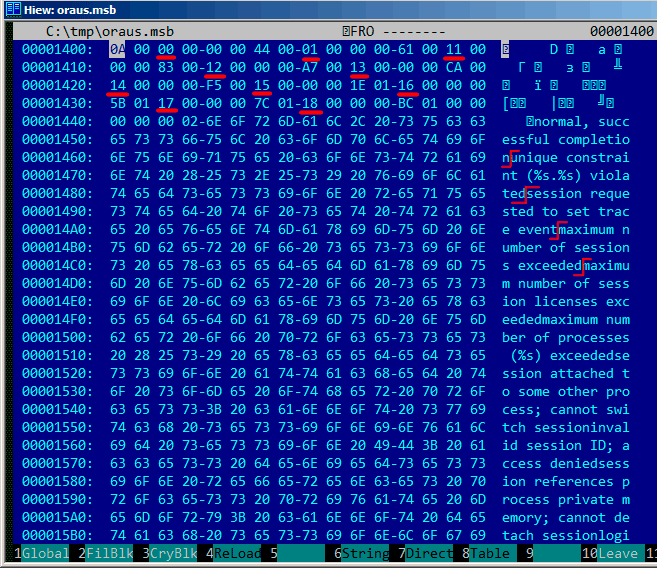
\includegraphics[width=0.6\textwidth]{examples/lines/2.png}
\caption{Practical joke works}
\end{figure}

Oh yes, it works\footnote{Author of this book once did this as a joke for his coworkers with 
the hope that they would stop playing. They didn't.}.

But why are the arguments to the \TT{random()} functions global variables?
That's just because it's possible to change the board size in the game's settings, 
so these values are not hardcoded.
The 10 and 5 values are just defaults.
}\RU{\clearpage
\section{Шутка с игрой Color Lines}
\label{chap:color_lines}

Это очень популярная игра с большим количеством реализаций.
Возьмем одну из них, с названием BallTriX, от 1997, доступную бесплатно на \url{http://go.yurichev.com/17311}
\footnote{Или на \url{http://go.yurichev.com/17365} или \url{http://go.yurichev.com/17366}.}.
Вот как она выглядит:

\begin{figure}[H]
\centering
\includegraphics[width=0.6\textwidth]{examples/lines/1.png}
\caption{Обычный вид игры}
\label{fig:lines_1}
\end{figure}

\clearpage
\myindex{\CStandardLibrary!rand()}
Посмотрим, сможем ли мы найти генератор псевдослучайных чисел и и сделать с ним одну шутку.

\IDA быстро распознает стандартную функцию \TT{\_rand} в 
\TT{balltrix.exe} по адресу \TT{0x00403DA0}.
\IDA также показывает, что она вызывается только из одного места:

\lstinputlisting[style=customasmx86]{examples/lines/random.lst}

Назовем её \q{random}.
Пока не будем концентрироваться на самом коде функции.

Эта функция вызывается из трех мест.

Вот первые два:

\lstinputlisting[style=customasmx86]{examples/lines/1.lst}

Вот третье:

\lstinputlisting[style=customasmx86]{examples/lines/2.lst}

Так что у функции только один аргумент.
10 передается в первых двух случаях и 5 в третьем.

Мы также можем заметить, что размер доски 10*10 и здесь 5 возможных цветов.
Это оно!
Стандартная функция \TT{rand()} возвращает число в пределах \TT{0..0x7FFF} и это неудобно, так что многие программисты пишут свою функцию,
возвращающую случайное число в некоторых заданных пределах.
В нашем случае, предел это $0..n-1$ и $n$ передается как
единственный аргумент в функцию.
Мы можем быстро проверить это в отладчике.

Сделаем так, чтобы третий вызов функции всегда возвращал ноль.
В начале заменим три инструкции (\TT{PUSH/CALL/ADD}) 
на \ac{NOP}s.
Затем добавим инструкцию \INS{XOR EAX, EAX}, для очистки регистра \EAX.

\lstinputlisting[style=customasmx86]{examples/lines/fixed.lst}

Что мы сделали, это заменили вызов функции \TT{random()} 
на код, всегда возвращающий ноль.

\clearpage
Теперь запустим:

\begin{figure}[H]
\centering
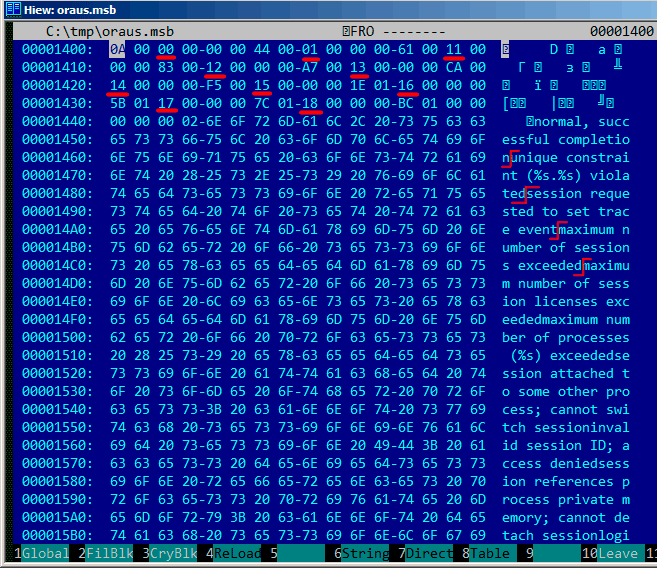
\includegraphics[width=0.6\textwidth]{examples/lines/2.png}
\caption{Шутка сработала}
\end{figure}

О да, это работает\footnote{Автор этой книги однажды сделал это как 
шутку для его сотрудников, в надежде что они перестанут играть. 
Надежды не оправдались.}.

Но почему аргументы функции \TT{random()} это глобальные переменные?
Это просто потому что в настройках игры можно изменять размер доски, так что эти параметры не фиксированы.
10 и 5 это просто значения по умолчанию.
}
\EN{\section{\MinesweeperWinXPExampleChapterName}
\label{minesweeper_winxp}
\myindex{Windows!Windows XP}

For those who are not very good at playing Minesweeper, we could try to reveal the hidden mines in the debugger.

\myindex{\CStandardLibrary!rand()}
\myindex{Windows!PDB}

As we know, Minesweeper places mines randomly, so there has to be some kind of random number generator or
a call to the standard \TT{rand()} C-function.

What is really cool about reversing Microsoft products is that there are \gls{PDB} 
file with symbols (function names, \etc{}).
When we load \TT{winmine.exe} into \IDA, it downloads the 
\gls{PDB} file exactly for this 
executable and shows all names.

So here it is, the only call to \TT{rand()} is this function:

\begin{lstlisting}[style=customasmx86]
.text:01003940 ; __stdcall Rnd(x)
.text:01003940 _Rnd@4          proc near               ; CODE XREF: StartGame()+53
.text:01003940                                         ; StartGame()+61
.text:01003940
.text:01003940 arg_0           = dword ptr  4
.text:01003940
.text:01003940                 call    ds:__imp__rand
.text:01003946                 cdq
.text:01003947                 idiv    [esp+arg_0]
.text:0100394B                 mov     eax, edx
.text:0100394D                 retn    4
.text:0100394D _Rnd@4          endp
\end{lstlisting}

\IDA named it so, and it was the name given to it by Minesweeper's developers.

The function is very simple:

\begin{lstlisting}[style=customc]
int Rnd(int limit)
{
    return rand() % limit;
};
\end{lstlisting}

(There is no \q{limit} name in the \gls{PDB} file; we manually named this argument like this.)

So it returns 
a random value from 0 to a specified limit.

\TT{Rnd()} is called only from one place, 
a function called \TT{StartGame()}, 
and as it seems, this is exactly 
the code which place the mines:

\begin{lstlisting}[style=customasmx86]
.text:010036C7                 push    _xBoxMac
.text:010036CD                 call    _Rnd@4          ; Rnd(x)
.text:010036D2                 push    _yBoxMac
.text:010036D8                 mov     esi, eax
.text:010036DA                 inc     esi
.text:010036DB                 call    _Rnd@4          ; Rnd(x)
.text:010036E0                 inc     eax
.text:010036E1                 mov     ecx, eax
.text:010036E3                 shl     ecx, 5          ; ECX=ECX*32
.text:010036E6                 test    _rgBlk[ecx+esi], 80h
.text:010036EE                 jnz     short loc_10036C7
.text:010036F0                 shl     eax, 5          ; EAX=EAX*32
.text:010036F3                 lea     eax, _rgBlk[eax+esi]
.text:010036FA                 or      byte ptr [eax], 80h
.text:010036FD                 dec     _cBombStart
.text:01003703                 jnz     short loc_10036C7
\end{lstlisting}

Minesweeper allows you to set the board size, so the X (xBoxMac) and Y (yBoxMac) of the board are global variables.
They are passed to \TT{Rnd()} and random 
coordinates are generated.
A mine is placed by the \TT{OR} instruction at \TT{0x010036FA}. 
And if it has been placed before 
(it's possible if the pair of \TT{Rnd()} 
generates a coordinates pair which has been already 
generated), 
then \TT{TEST} and \TT{JNZ} at \TT{0x010036E6} 
jumps to the generation routine again.

\TT{cBombStart} is the global variable containing total number of mines. So this is loop.

The width of the array is 32 
(we can conclude this by looking at the \TT{SHL} instruction, which multiplies one of the coordinates by 32).

The size of the \TT{rgBlk} 
global array can be easily determined by the difference 
between the \TT{rgBlk} 
label in the data segment and the next known one. 
It is 0x360 (864):

\begin{lstlisting}[style=customasmx86]
.data:01005340 _rgBlk          db 360h dup(?)          ; DATA XREF: MainWndProc(x,x,x,x)+574
.data:01005340                                         ; DisplayBlk(x,x)+23
.data:010056A0 _Preferences    dd ?                    ; DATA XREF: FixMenus()+2
...
\end{lstlisting}

$864/32=27$.

So the array size is $27*32$?
It is close to what we know: when we try to set board size to $100*100$ in Minesweeper settings, it fallbacks to a board of size $24*30$.
So this is the maximal board size here.
And the array has a fixed size for any board size.

So let's see all this in \olly.
We will ran Minesweeper, attaching \olly to it and now we can see the memory dump at the address of the \TT{rgBlk} array (\TT{0x01005340})
\footnote{All addresses here are for Minesweeper for Windows XP SP3 English. 
They may differ for other service packs.}.

So we got this memory dump of the array:

\lstinputlisting[style=customasmx86]{examples/minesweeper/1.lst}

\olly, like any other hexadecimal editor, shows 16 bytes per line.
So each 32-byte array row occupies exactly 2 lines here.

This is beginner level (9*9 board).

There is some square 
structure can be seen visually (0x10 bytes).

We will click \q{Run} in \olly to unfreeze the Minesweeper process, then we'll clicked randomly at the Minesweeper window 
and trapped into mine, but now all mines are visible:

\begin{figure}[H]
\centering
\myincludegraphicsSmall{examples/minesweeper/1.png}
\caption{Mines}
\label{fig:minesweeper1}
\end{figure}

By comparing the mine places and the dump, we can conclude that 0x10 stands for border, 0x0F---empty block, 0x8F---mine.

Now we'll add comments and also enclose all 0x8F bytes into square brackets:

\lstinputlisting[style=customasmx86]{examples/minesweeper/2.lst}

Now we'll remove all \IT{border bytes} (0x10) and what's beyond those:

\lstinputlisting[style=customasmx86]{examples/minesweeper/3.lst}

Yes, these are mines, now it can be clearly seen and compared with the screenshot.

\clearpage
What is interesting is that we can modify the array right in \olly.
We can remove all mines by changing all 0x8F bytes by 0x0F, and here is what we'll get in Minesweeper:

\begin{figure}[H]
\centering
\myincludegraphicsSmall{examples/minesweeper/3.png}
\caption{All mines are removed in debugger}
\label{fig:minesweeper3}
\end{figure}

We can also move all of them to the first line: 

\begin{figure}[H]
\centering
\myincludegraphicsSmall{examples/minesweeper/2.png}
\caption{Mines set in debugger}
\label{fig:minesweeper2}
\end{figure}

Well, the debugger is not very convenient for eavesdropping (which is our goal anyway), so we'll write a small utility
to dump the contents of the board:

\lstinputlisting[style=customc]{examples/minesweeper/minesweeper_cheater.c}

Just set the \ac{PID}
\footnote{PID it can be seen in Task Manager 
(enable it in \q{View $\rightarrow$ Select Columns})} 
and the address of the array (\TT{0x01005340} for Windows XP SP3 English) 
and it will dump it
\footnote{The compiled executable is here: 
\href{http://go.yurichev.com/17165}{beginners.re}}.

It attaches itself to a win32 process by \ac{PID} and just reads process memory an the address.

\subsection{Finding grid automatically}

This is kind of nuisance to set address each time when we run our utility.
Also, various Minesweeper versions may have the array on different address.
Knowing the fact that there is always a border (0x10 bytes), we can just find it in memory:

\lstinputlisting[style=customc]{examples/minesweeper/cheater2_fragment.c}

Full source code: \url{https://github.com/dennis714/RE-for-beginners/blob/master/examples/minesweeper/minesweeper_cheater2.c}.

\subsection{\Exercises}

\begin{itemize}

\item 
Why do the \IT{border bytes} (0x10) exist in the array?

What they are for if they are not visible in Minesweeper's interface?
How could it work without them?

\item 
As it turns out, there are more values possible (for open blocks, for flagged by user, \etc{}).
Try to find the meaning of each one.

\item 
Modify my utility so it can remove all mines or set them in a fixed pattern that you want in the Minesweeper
process currently running.

\end{itemize}
}\RU{\section{\MinesweeperWinXPExampleChapterName}
\label{minesweeper_winxp}
\myindex{Windows!Windows XP}

Для тех, кто не очень хорошо играет в Сапёра (Minesweeper), можно попробовать найти все скрытые мины в отладчике.

\myindex{\CStandardLibrary!rand()}
\myindex{Windows!PDB}
Как мы знаем, Сапёр располагает мины случайным образом, так что там должен быть генератор случайных чисел
или вызов стандартной функции Си \TT{rand()}.

Вот что хорошо в реверсинге продуктов от Microsoft, так это то что часто есть \gls{PDB}-файл со всеми
символами (имена функций, \etc{}.).

Когда мы загружаем \TT{winmine.exe} в \IDA, она скачивает 
\gls{PDB} файл именно для этого исполняемого файла и добавляет все имена.

И вот оно, только один вызов \TT{rand()} в этой функции:

\begin{lstlisting}[style=customasmx86]
.text:01003940 ; __stdcall Rnd(x)
.text:01003940 _Rnd@4          proc near               ; CODE XREF: StartGame()+53
.text:01003940                                         ; StartGame()+61
.text:01003940
.text:01003940 arg_0           = dword ptr  4
.text:01003940
.text:01003940                 call    ds:__imp__rand
.text:01003946                 cdq
.text:01003947                 idiv    [esp+arg_0]
.text:0100394B                 mov     eax, edx
.text:0100394D                 retn    4
.text:0100394D _Rnd@4          endp
\end{lstlisting}

Так её назвала \IDA и это было имя данное ей разработчиками Сапёра.

Функция очень простая:

\begin{lstlisting}[style=customc]
int Rnd(int limit)
{
    return rand() % limit;
};
\end{lstlisting}

(В \gls{PDB}-файле не было имени \q{limit}; это мы назвали этот аргумент так, вручную.)

Так что она возвращает случайное число в пределах от нуля до заданного предела.

\TT{Rnd()} вызывается только из одного места, это функция с названием \TT{StartGame()}, 
и как видно, это именно тот код, что расставляет мины:

\begin{lstlisting}[style=customasmx86]
.text:010036C7                 push    _xBoxMac
.text:010036CD                 call    _Rnd@4          ; Rnd(x)
.text:010036D2                 push    _yBoxMac
.text:010036D8                 mov     esi, eax
.text:010036DA                 inc     esi
.text:010036DB                 call    _Rnd@4          ; Rnd(x)
.text:010036E0                 inc     eax
.text:010036E1                 mov     ecx, eax
.text:010036E3                 shl     ecx, 5          ; ECX=ECX*32
.text:010036E6                 test    _rgBlk[ecx+esi], 80h
.text:010036EE                 jnz     short loc_10036C7
.text:010036F0                 shl     eax, 5          ; EAX=EAX*32
.text:010036F3                 lea     eax, _rgBlk[eax+esi]
.text:010036FA                 or      byte ptr [eax], 80h
.text:010036FD                 dec     _cBombStart
.text:01003703                 jnz     short loc_10036C7
\end{lstlisting}

Сапёр позволяет задать размеры доски, так что X (xBoxMac) и Y (yBoxMac) это глобальные переменные.

Они передаются в \TT{Rnd()} и генерируются случайные координаты.
Мина устанавливается инструкцией \TT{OR} на \TT{0x010036FA}. 
И если она уже была установлена до этого 
(это возможно, если пара функций \TT{Rnd()} 
сгенерирует пару, которая уже была сгенерирована), 
тогда \TT{TEST} и \TT{JNZ} на \TT{0x010036E6} 
перейдет на повторную генерацию пары.

\TT{cBombStart} это глобальная переменная, содержащая количество мин. Так что это цикл.

Ширина двухмерного массива это 32 (мы можем это вывести, глядя на инструкцию \TT{SHL}, которая умножает
одну из координат на 32).

Размер глобального массива \TT{rgBlk} 
можно легко узнать по разнице между меткой \TT{rgBlk} 
в сегменте данных и следующей известной меткой. 
Это 0x360 (864):

\begin{lstlisting}[style=customasmx86]
.data:01005340 _rgBlk          db 360h dup(?)          ; DATA XREF: MainWndProc(x,x,x,x)+574
.data:01005340                                         ; DisplayBlk(x,x)+23
.data:010056A0 _Preferences    dd ?                    ; DATA XREF: FixMenus()+2
...
\end{lstlisting}

$864/32=27$.

Так что размер массива $27*32$?
Это близко к тому что мы знаем: если попытаемся установить размер доски в установках Сапёра на $100*100$, то он установит размер $24*30$.
Так что это максимальный размер доски здесь.
И размер массива фиксирован для доски любого размера.

Посмотрим на всё это в \olly.
Запустим Сапёр, присоединим (attach) \olly к нему и увидим содержимое памяти по адресу где массив \TT{rgBlk} (\TT{0x01005340})%

\footnote{Все адреса здесь для Сапёра под Windows XP SP3 English. 
Они могут отличаться для других сервис-паков.}.

Так что у нас выходит такой дамп памяти массива:

\lstinputlisting[style=customasmx86]{examples/minesweeper/1.lst}

\olly, как и любой другой шестнадцатеричный редактор, показывает 16 байт на строку.
Так что каждая 32-байтная строка массива занимает ровно 2 строки.

Это уровень для начинающих (доска 9*9).

Тут еще какая-то квадратная структура, заметная визуально (байты 0x10).

Нажмем \q{Run} в \olly чтобы разморозить процесс Сапёра, потом нажмем в случайное место окна Сапёра, попадаемся на мине, но теперь
видны все мины:

\begin{figure}[H]
\centering
\myincludegraphicsSmall{examples/minesweeper/1.png}
\caption{Мины}
\label{fig:minesweeper1}
\end{figure}

Сравнивая места с минами и дамп, мы можем обнаружить что 0x10 это граница, 0x0F --- пустой блок, 
0x8F --- мина.

Теперь добавим комментариев и также заключим все байты 0x8F в квадратные скобки:%

\lstinputlisting[style=customasmx86]{examples/minesweeper/2.lst}

Теперь уберем все байты связанные с границами (0x10) и всё что за ними:%

\lstinputlisting[style=customasmx86]{examples/minesweeper/3.lst}

Да, это всё мины, теперь это очень хорошо видно, в сравнении со скриншотом.

\clearpage
Вот что интересно, это то что мы можем модифицировать массив прямо в \olly.%

Уберем все мины заменив все байты 0x8F на 0x0F, и вот что получится в Сапёре:

\begin{figure}[H]
\centering
\myincludegraphicsSmall{examples/minesweeper/3.png}
\caption{Все мины убраны в отладчике}
\label{fig:minesweeper3}
\end{figure}

Также уберем их все и добавим их в первом ряду: 

\begin{figure}[H]
\centering
\myincludegraphicsSmall{examples/minesweeper/2.png}
\caption{Мины, установленные в отладчике}
\label{fig:minesweeper2}
\end{figure}

Отладчик не очень удобен для подсматривания (а это была наша изначальная цель), так что напишем маленькую
утилиту для показа содержимого доски:

\lstinputlisting[style=customc]{examples/minesweeper/minesweeper_cheater.c}

Просто установите \ac{PID}
\footnote{PID можно увидеть в Task Manager 
(это можно включить в \q{View $\rightarrow$ Select Columns})} 
и адрес массива (\TT{0x01005340} для Windows XP SP3 English) 
и она покажет его
\footnote{Скомпилированная версия здесь: 
\href{http://go.yurichev.com/17165}{beginners.re}}.

Она подключается к win32-процессу по \ac{PID}-у и просто читает из памяти процесса по этому адресу.

\subsection{Автоматический поиск массива}

Здавать адрес каждый раз при запуске нашей утилиты, это неудобно.
К тому же, разные версии ``Сапёра'' могут иметь этот массив по разным адресам.
Зная, что всегда есть рамка (байты 0x10), массив легко найти в памяти:

\lstinputlisting[style=customc]{examples/minesweeper/cheater2_fragment.c}

Полный исходный код: \url{https://github.com/dennis714/RE-for-beginners/blob/master/examples/minesweeper/minesweeper_cheater2.c}.

\subsection{\Exercises}

\begin{itemize}

\item
Почему байты описывающие границы (0x10) присутствуют вообще?
Зачем они нужны, если они вообще не видимы в интерфейсе Сапёра?
Как можно обойтись без них?

\item
Как выясняется, здесь больше возможных значений (для открытых блоков, для тех на которых игрок установил
флажок, \etc{}.).
	
Попробуйте найти значение каждого.

\item Измените мою утилиту так, чтобы она в запущенном процессе Сапёра убирала все мины, 
или расставляла их в соответствии с каким-то заданным шаблоном.

\end{itemize}
}
\EN{\section{Hacking Windows clock}

Sometimes I did some kind of first April prank for my coworkers.

Let's find, if we could do something with Windows clock?
Can we force to go clock hands backwards?

First of all, when you click on date/time in status bar,\\
a \IT{C:\textbackslash{}WINDOWS\textbackslash{}SYSTEM32\textbackslash{}TIMEDATE.CPL} module gets executed,
which is usual executable PE file.

Let's see, how it draw hands?
When I open the file (from Windows 7) in Resource Hacker, there are clock faces, but with no hands:

\begin{figure}[H]
\centering
\myincludegraphics{examples/timedate/reshack.png}
\caption{Resource Hacker}
\end{figure}

OK, what we know? How to draw a clock hand? All they are started at the middle of circle, ending with its border.
Hence, we must calculate coordinates of a point on circle's border.
From school-level mathematics we may recall that we have to use sine/cosine functions to draw circle, or at least
square root.
There are no such things in \IT{TIMEDATE.CPL}, at least at first glance.
But, thanks to Microsoft debugging PDB files, I can find a function named \IT{CAnalogClock::DrawHand()}, which calls
\IT{Gdiplus::Graphics::DrawLine()} at least twice.

Here is its code:

\lstinputlisting[style=customasmx86]{examples/timedate/1.lst}

\myindex{Windows!Win32!MulDiv()}
We can see that \IT{DrawLine()} arguments are dependent on result of \IT{MulDiv()} function
and a \IT{table[]} table (name is mine),
which has 8-byte elements (look at \INS{LEA}'s second operand).

What is inside of table[]?

\lstinputlisting[style=customasmx86]{examples/timedate/2.lst}

It's referenced only from \IT{DrawHand()} function at has 120 32-bit words or 60 32-bit pairs... wait, 60?
Let's take a closer look at these values.
First of all, I'll zap 6 pairs or 12 32-bit words with zeros, and then I'll put patched \IT{TIMEDATE.CPL}
into \IT{C:\textbackslash{}WINDOWS\textbackslash{}SYSTEM32}.
(You may need to set owner of the *TIMEDATE.CPL* file to your primary user account (instead of \IT{TrustedInstaller}),
and also, boot in safe mode with command prompt so you can copy the file, which is usually locked.)

\begin{figure}[H]
\centering
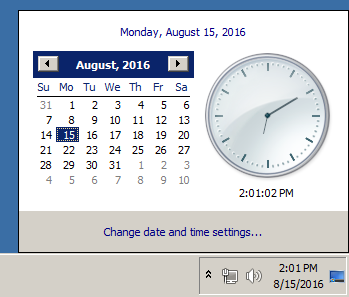
\includegraphics[width=0.5\textwidth]{examples/timedate/6_pairs_zeroed.png}
\caption{Attempt to run}
\end{figure}

Now when any hand is located at 0-5 seconds/minutes, it's invisible! However, opposite (shorter) part of second hand
is visible and moving.
When any hand is outside of this area, hand is visible as usual.

\myindex{Mathematica}
Let's take even closer look at the table in Mathematica.
I have copypasted table from the \IT{TIMEDATE.CPL} to a \IT{tbl} file (480 bytes).
We will take for granted the fact that these are signed values, because half of elements are below zero (0FFFFE0C1h, etc.).
If these values would be unsigned, they would be suspiciously huge.

\begin{lstlisting}[style=custommath]
In[]:= tbl = BinaryReadList["~/.../tbl", "Integer32"]

Out[]= {0, -7999, 836, -7956, 1663, -7825, 2472, -7608, 3253, -7308, 3999, \
-6928, 4702, -6472, 5353, -5945, 5945, -5353, 6472, -4702, 6928, \
-4000, 7308, -3253, 7608, -2472, 7825, -1663, 7956, -836, 8000, 0, \
7956, 836, 7825, 1663, 7608, 2472, 7308, 3253, 6928, 4000, 6472, \
4702, 5945, 5353, 5353, 5945, 4702, 6472, 3999, 6928, 3253, 7308, \
2472, 7608, 1663, 7825, 836, 7956, 0, 7999, -836, 7956, -1663, 7825, \
-2472, 7608, -3253, 7308, -4000, 6928, -4702, 6472, -5353, 5945, \
-5945, 5353, -6472, 4702, -6928, 3999, -7308, 3253, -7608, 2472, \
-7825, 1663, -7956, 836, -7999, 0, -7956, -836, -7825, -1663, -7608, \
-2472, -7308, -3253, -6928, -4000, -6472, -4702, -5945, -5353, -5353, \
-5945, -4702, -6472, -3999, -6928, -3253, -7308, -2472, -7608, -1663, \
-7825, -836, -7956}

In[]:= Length[tbl]
Out[]= 120
\end{lstlisting}

Let's treat two consecutive 32-bit values as pair:

\begin{lstlisting}[style=custommath]
In[]:= pairs = Partition[tbl, 2]
Out[]= {{0, -7999}, {836, -7956}, {1663, -7825}, {2472, -7608}, \
{3253, -7308}, {3999, -6928}, {4702, -6472}, {5353, -5945}, {5945, \
-5353}, {6472, -4702}, {6928, -4000}, {7308, -3253}, {7608, -2472}, \
{7825, -1663}, {7956, -836}, {8000, 0}, {7956, 836}, {7825, 
1663}, {7608, 2472}, {7308, 3253}, {6928, 4000}, {6472, 
4702}, {5945, 5353}, {5353, 5945}, {4702, 6472}, {3999, 
6928}, {3253, 7308}, {2472, 7608}, {1663, 7825}, {836, 7956}, {0, 
7999}, {-836, 7956}, {-1663, 7825}, {-2472, 7608}, {-3253, 
7308}, {-4000, 6928}, {-4702, 6472}, {-5353, 5945}, {-5945, 
5353}, {-6472, 4702}, {-6928, 3999}, {-7308, 3253}, {-7608, 
2472}, {-7825, 1663}, {-7956, 836}, {-7999, 
0}, {-7956, -836}, {-7825, -1663}, {-7608, -2472}, {-7308, -3253}, \
{-6928, -4000}, {-6472, -4702}, {-5945, -5353}, {-5353, -5945}, \
{-4702, -6472}, {-3999, -6928}, {-3253, -7308}, {-2472, -7608}, \
{-1663, -7825}, {-836, -7956}}

In[]:= Length[pairs]
Out[]= 60
\end{lstlisting}

Let's try to treat each pair as X/Y coordinate and draw all 60 pairs, and also first 15 pairs:

\begin{figure}[H]
\centering
\myincludegraphics{examples/timedate/math.png}
\caption{Mathematica}
\end{figure}

Now this is something!
Each pair is just coordinate.
First 15 pairs are coordinates for $\frac{1}{4}$ of circle.

Perhaps, Microsoft developers precalculated all coordinates and put them into table.

Now I can understand why when I zapped 6 pairs, hands were invisible at that area: in fact, hands were drawn,
they just had zero length, because hand started at 0:0 coordinate and ended there.

\subsubsection{The prank (practical joke)}

Given all that, how would we force hands to go counterclockwise?
In fact, this is simple, we need just to rotate the table, so each hand, instead of drawing at place of first second,
would be drawing at place of 59th second.

I made the patcher a long time ago, at the very beginning of 2000s, for Windows 2000.
Hard to believe, it still works for Windows 7, perhaps, the table hasn't been changed since then!

Patcher source code: \url{https://github.com/dennis714/random_notes/blob/master/timedate/time_pt.c}.

Now I can see all hands goes backwards:

\begin{figure}[H]
\centering
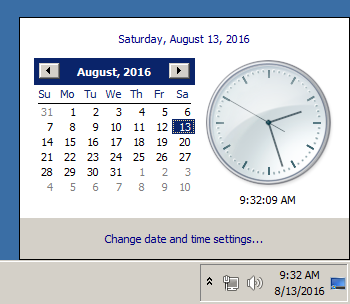
\includegraphics[width=0.5\textwidth]{examples/timedate/counterclockwise.png}
\caption{Now it works}
\end{figure}

Well, there is no animation in this article, but if you look closer, you can see, that hands are in fact shows correct
time, but the whole clock face is rotated vertically, like we see it from the inside of clock.

\subsubsection{Windows 2000 leaked source code}

So I did the patcher and then Windows 2000 source code has been leaked (I can't force you to trust me, though).
Let's take a look on source code if that function and table.\\
The file is \IT{win2k/private/shell/cpls/utc/clock.c}:

\begin{lstlisting}[style=customc]
//
//  Array containing the sine and cosine values for hand positions.
//
POINT rCircleTable[] =
{
    { 0,     -7999},
    { 836,   -7956},
    { 1663,  -7825},
    { 2472,  -7608},
    { 3253,  -7308},
...
    { -4702, -6472},
    { -3999, -6928},
    { -3253, -7308},
    { -2472, -7608},
    { -1663, -7825},
    { -836 , -7956},
};

////////////////////////////////////////////////////////////////////////////
//
//  DrawHand
//
//  Draws the hands of the clock.
//
////////////////////////////////////////////////////////////////////////////

void DrawHand(
    HDC hDC,
    int pos,
    HPEN hPen,
    int scale,
    int patMode,
    PCLOCKSTR np)
{
    LPPOINT lppt;
    int radius;

    MoveTo(hDC, np->clockCenter.x, np->clockCenter.y);
    radius = MulDiv(np->clockRadius, scale, 100);
    lppt = rCircleTable + pos;
    SetROP2(hDC, patMode);
    SelectObject(hDC, hPen);

    LineTo( hDC,
            np->clockCenter.x + MulDiv(lppt->x, radius, 8000),
            np->clockCenter.y + MulDiv(lppt->y, radius, 8000) );
}
\end{lstlisting}

Now it's clear: coordinates has been precalculated as if clock face has height and width of $2 \cdot 8000$,
and then it's rescaled to current clock face radius using \IT{MulDiv()} function.

POINT structure\footnote{\url{https://msdn.microsoft.com/en-us/library/windows/desktop/dd162805(v=vs.85).aspx}}
is a structure of two 32-bit values, first is \IT{x}, second is \IT{y}.

}
\section{\RU{Донглы}\EN{Dongles}}
\label{dongles}

\RU{Автор этих строк иногда делал замену \glslink{dongle}{донглам} или \q{эмуляторы донглов} 
и здесь немного примеров, как это происходит.}
\EN{The author of these lines, occasionally did software copy-protection \gls{dongle} replacements, or \q{dongle emulators} and here
are couple examples of how it's happening.}

\RU{Об одном неописанном здесь случае с Rockey и Z3 вы также можете прочитать здесь}
\EN{About one of the cases about Rocket and Z3 that is not present here, you can read here}:
\url{http://yurichev.com/tmp/SAT_SMT_DRAFT.pdf}.

\EN{\input{examples/dongles/1/main_EN}}\RU{\input{examples/dongles/1/main_RU}}
\EN{\input{examples/dongles/2/main_EN}}\RU{\input{examples/dongles/2/main_RU}}
\EN{\input{examples/dongles/3/main_EN}}\RU{\input{examples/dongles/3/main_RU}}


\EN{\section{
\q{QR9}: Rubik's cube inspired amateur crypto-algorithm}

Sometimes amateur cryptosystems appear to be pretty bizarre.

The author of this book was once asked to reverse engineer an amateur cryptoalgorithm of some data encryption utility, 
the source code for which was lost\footnote{He also got permission from the customer to publish the algorithm's details}.

Here is the listing exported from \IDA for the original encryption utility:

\lstinputlisting[style=customasmx86]{examples/qr9/qr9_original.lst}

All function and label names were given by me during the analysis.

Let's start from the top. Here is a function that takes two file names and password.

\begin{lstlisting}[style=customasmx86]
.text:00541320 ; int __cdecl crypt_file(int Str, char *Filename, int password)
.text:00541320 crypt_file      proc near
.text:00541320
.text:00541320 Str             = dword ptr  4
.text:00541320 Filename        = dword ptr  8
.text:00541320 password        = dword ptr  0Ch
.text:00541320
\end{lstlisting}

Open the file and report if an error occurs:

\begin{lstlisting}[style=customasmx86]
.text:00541320                 mov     eax, [esp+Str]
.text:00541324                 push    ebp
.text:00541325                 push    offset Mode     ; "rb"
.text:0054132A                 push    eax             ; Filename
.text:0054132B                 call    _fopen          ; open file
.text:00541330                 mov     ebp, eax
.text:00541332                 add     esp, 8
.text:00541335                 test    ebp, ebp
.text:00541337                 jnz     short loc_541348
.text:00541339                 push    offset Format   ; "Cannot open input file!\n"
.text:0054133E                 call    _printf
.text:00541343                 add     esp, 4
.text:00541346                 pop     ebp
.text:00541347                 retn
.text:00541348
.text:00541348 loc_541348:
\end{lstlisting}

\myindex{\CStandardLibrary!fseek()}
\myindex{\CStandardLibrary!ftell()}
Get the file size via \TT{fseek()}/\TT{ftell()}:

\lstinputlisting[style=customasmx86]{examples/qr9/1_EN}

This fragment of code calculates the file size aligned on a 64-byte boundary. 
This is because this cryptographic algorithm works with only 64-byte blocks. 
The operation is pretty straightforward: divide the file size by 64, forget about the remainder and add 1, 
then multiply by 64. 
The following code removes the remainder as if the value has already been divided by 64 and adds 64. 
It is almost the same.

\lstinputlisting[style=customasmx86]{examples/qr9/2_EN}

Allocate buffer with aligned size:

\begin{lstlisting}[style=customasmx86]
.text:00541373                 push    esi             ; Size
.text:00541374                 call    _malloc
\end{lstlisting}

\myindex{\CStandardLibrary!calloc()}
Call memset(), e.g., clear the allocated buffer\footnote{malloc() + memset() could 
be replaced by calloc()}.

\lstinputlisting[style=customasmx86]{examples/qr9/3_EN}

Read file via the standard C function \TT{fread()}.

\begin{lstlisting}[style=customasmx86]
.text:00541392                 mov     eax, [esp+38h+Str]
.text:00541396                 push    eax             ; ElementSize
.text:00541397                 push    ebx             ; DstBuf
.text:00541398                 call    _fread          ; read file
.text:0054139D                 push    ebp             ; File
.text:0054139E                 call    _fclose
\end{lstlisting}

Call \TT{crypt()}. This function takes a buffer, buffer size (aligned) and a password string.

\begin{lstlisting}[style=customasmx86]
.text:005413A3                 mov     ecx, [esp+44h+password]
.text:005413A7                 push    ecx             ; password
.text:005413A8                 push    esi             ; aligned size
.text:005413A9                 push    ebx             ; buffer
.text:005413AA                 call    crypt           ; do crypt
\end{lstlisting}

Create the output file. By the way, the developer forgot to check if it has been created correctly! 
The file opening result is being checked, though.

\begin{lstlisting}[style=customasmx86]
.text:005413AF                 mov     edx, [esp+50h+Filename]
.text:005413B3                 add     esp, 40h
.text:005413B6                 push    offset aWb      ; "wb"
.text:005413BB                 push    edx             ; Filename
.text:005413BC                 call    _fopen
.text:005413C1                 mov     edi, eax
\end{lstlisting}

The newly created file handle is in the \EDI register now. Write signature \q{QR9}.

\begin{lstlisting}[style=customasmx86]
.text:005413C3                 push    edi             ; File
.text:005413C4                 push    1               ; Count
.text:005413C6                 push    3               ; Size
.text:005413C8                 push    offset aQr9     ; "QR9"
.text:005413CD                 call    _fwrite         ; write file signature
\end{lstlisting}

Write the actual file size (not aligned):

\begin{lstlisting}[style=customasmx86]
.text:005413D2                 push    edi             ; File
.text:005413D3                 push    1               ; Count
.text:005413D5                 lea     eax, [esp+30h+Str]
.text:005413D9                 push    4               ; Size
.text:005413DB                 push    eax             ; Str
.text:005413DC                 call    _fwrite         ; write original file size
\end{lstlisting}

Write the encrypted buffer:

\begin{lstlisting}[style=customasmx86]
.text:005413E1                 push    edi             ; File
.text:005413E2                 push    1               ; Count
.text:005413E4                 push    esi             ; Size
.text:005413E5                 push    ebx             ; Str
.text:005413E6                 call    _fwrite         ; write encrypted file
\end{lstlisting}

Close the file and free the allocated buffer:

\begin{lstlisting}[style=customasmx86]
.text:005413EB                 push    edi             ; File
.text:005413EC                 call    _fclose
.text:005413F1                 push    ebx             ; Memory
.text:005413F2                 call    _free
.text:005413F7                 add     esp, 40h
.text:005413FA                 pop     edi
.text:005413FB                 pop     esi
.text:005413FC                 pop     ebx
.text:005413FD                 pop     ebp
.text:005413FE                 retn
.text:005413FE crypt_file      endp
\end{lstlisting}

Here is the reconstructed C code:

\begin{lstlisting}[style=customc]
void crypt_file(char *fin, char* fout, char *pw)
{
	FILE *f;
	int flen, flen_aligned;
	BYTE *buf;

	f=fopen(fin, "rb");
	
	if (f==NULL)
	{
		printf ("Cannot open input file!\n");
		return;
	};

	fseek (f, 0, SEEK_END);
	flen=ftell (f);
	fseek (f, 0, SEEK_SET);

	flen_aligned=(flen&0xFFFFFFC0)+0x40;

	buf=(BYTE*)malloc (flen_aligned);
	memset (buf, 0, flen_aligned);

	fread (buf, flen, 1, f);

	fclose (f);

	crypt (buf, flen_aligned, pw);
	
	f=fopen(fout, "wb");

	fwrite ("QR9", 3, 1, f);
	fwrite (&flen, 4, 1, f);
	fwrite (buf, flen_aligned, 1, f);

	fclose (f);

	free (buf);
};
\end{lstlisting}

The decryption procedure is almost the same:

\begin{lstlisting}[style=customasmx86]
.text:00541400 ; int __cdecl decrypt_file(char *Filename, int, void *Src)
.text:00541400 decrypt_file    proc near
.text:00541400
.text:00541400 Filename        = dword ptr  4
.text:00541400 arg_4           = dword ptr  8
.text:00541400 Src             = dword ptr  0Ch
.text:00541400
.text:00541400                 mov     eax, [esp+Filename]
.text:00541404                 push    ebx
.text:00541405                 push    ebp
.text:00541406                 push    esi
.text:00541407                 push    edi
.text:00541408                 push    offset aRb      ; "rb"
.text:0054140D                 push    eax             ; Filename
.text:0054140E                 call    _fopen
.text:00541413                 mov     esi, eax
.text:00541415                 add     esp, 8
.text:00541418                 test    esi, esi
.text:0054141A                 jnz     short loc_54142E
.text:0054141C                 push    offset aCannotOpenIn_0 ; "Cannot open input file!\n"
.text:00541421                 call    _printf
.text:00541426                 add     esp, 4
.text:00541429                 pop     edi
.text:0054142A                 pop     esi
.text:0054142B                 pop     ebp
.text:0054142C                 pop     ebx
.text:0054142D                 retn
.text:0054142E
.text:0054142E loc_54142E:
.text:0054142E                 push    2               ; Origin
.text:00541430                 push    0               ; Offset
.text:00541432                 push    esi             ; File
.text:00541433                 call    _fseek
.text:00541438                 push    esi             ; File
.text:00541439                 call    _ftell
.text:0054143E                 push    0               ; Origin
.text:00541440                 push    0               ; Offset
.text:00541442                 push    esi             ; File
.text:00541443                 mov     ebp, eax
.text:00541445                 call    _fseek
.text:0054144A                 push    ebp             ; Size
.text:0054144B                 call    _malloc
.text:00541450                 push    esi             ; File
.text:00541451                 mov     ebx, eax
.text:00541453                 push    1               ; Count
.text:00541455                 push    ebp             ; ElementSize
.text:00541456                 push    ebx             ; DstBuf
.text:00541457                 call    _fread
.text:0054145C                 push    esi             ; File
.text:0054145D                 call    _fclose
\end{lstlisting}

Check signature (first 3 bytes):

\begin{lstlisting}[style=customasmx86]
.text:00541462                 add     esp, 34h
.text:00541465                 mov     ecx, 3
.text:0054146A                 mov     edi, offset aQr9_0 ; "QR9"
.text:0054146F                 mov     esi, ebx
.text:00541471                 xor     edx, edx
.text:00541473                 repe cmpsb
.text:00541475                 jz      short loc_541489
\end{lstlisting}

Report an error if the signature is absent:

\begin{lstlisting}[style=customasmx86]
.text:00541477                 push    offset aFileIsNotCrypt ; "File is not encrypted!\n"
.text:0054147C                 call    _printf
.text:00541481                 add     esp, 4
.text:00541484                 pop     edi
.text:00541485                 pop     esi
.text:00541486                 pop     ebp
.text:00541487                 pop     ebx
.text:00541488                 retn
.text:00541489
.text:00541489 loc_541489:
\end{lstlisting}

Call \TT{decrypt()}.

\begin{lstlisting}[style=customasmx86]
.text:00541489                 mov     eax, [esp+10h+Src]
.text:0054148D                 mov     edi, [ebx+3]
.text:00541490                 add     ebp, 0FFFFFFF9h
.text:00541493                 lea     esi, [ebx+7]
.text:00541496                 push    eax             ; Src
.text:00541497                 push    ebp             ; int
.text:00541498                 push    esi             ; int
.text:00541499                 call    decrypt
.text:0054149E                 mov     ecx, [esp+1Ch+arg_4]
.text:005414A2                 push    offset aWb_0    ; "wb"
.text:005414A7                 push    ecx             ; Filename
.text:005414A8                 call    _fopen
.text:005414AD                 mov     ebp, eax
.text:005414AF                 push    ebp             ; File
.text:005414B0                 push    1               ; Count
.text:005414B2                 push    edi             ; Size
.text:005414B3                 push    esi             ; Str
.text:005414B4                 call    _fwrite
.text:005414B9                 push    ebp             ; File
.text:005414BA                 call    _fclose
.text:005414BF                 push    ebx             ; Memory
.text:005414C0                 call    _free
.text:005414C5                 add     esp, 2Ch
.text:005414C8                 pop     edi
.text:005414C9                 pop     esi
.text:005414CA                 pop     ebp
.text:005414CB                 pop     ebx
.text:005414CC                 retn
.text:005414CC decrypt_file    endp
\end{lstlisting}

Here is the reconstructed C code:

\begin{lstlisting}[style=customc]
void decrypt_file(char *fin, char* fout, char *pw)
{
	FILE *f;
	int real_flen, flen;
	BYTE *buf;

	f=fopen(fin, "rb");
	
	if (f==NULL)
	{
		printf ("Cannot open input file!\n");
		return;
	};

	fseek (f, 0, SEEK_END);
	flen=ftell (f);
	fseek (f, 0, SEEK_SET);

	buf=(BYTE*)malloc (flen);

	fread (buf, flen, 1, f);

	fclose (f);

	if (memcmp (buf, "QR9", 3)!=0)
	{
		printf ("File is not encrypted!\n");
		return;
	};

	memcpy (&real_flen, buf+3, 4);

	decrypt (buf+(3+4), flen-(3+4), pw);
	
	f=fopen(fout, "wb");

	fwrite (buf+(3+4), real_flen, 1, f);

	fclose (f);

	free (buf);
};
\end{lstlisting}

OK, now let's go deeper.

Function \TT{crypt()}:

\begin{lstlisting}[style=customasmx86]
.text:00541260 crypt           proc near
.text:00541260
.text:00541260 arg_0           = dword ptr  4
.text:00541260 arg_4           = dword ptr  8
.text:00541260 arg_8           = dword ptr  0Ch
.text:00541260
.text:00541260                 push    ebx
.text:00541261                 mov     ebx, [esp+4+arg_0]
.text:00541265                 push    ebp
.text:00541266                 push    esi
.text:00541267                 push    edi
.text:00541268                 xor     ebp, ebp
.text:0054126A
.text:0054126A loc_54126A:
\end{lstlisting}

\myindex{x86!\Instructions!MOVSD}
This fragment of code copies a part of the input buffer to an internal array we later name \q{cube64}.
The size is in the \ECX register. \TT{MOVSD} stands for \IT{move 32-bit dword}, so, 
16 32-bit dwords are exactly 64 bytes.

\begin{lstlisting}[style=customasmx86]
.text:0054126A                 mov     eax, [esp+10h+arg_8]
.text:0054126E                 mov     ecx, 10h
.text:00541273                 mov     esi, ebx   ; EBX is pointer within input buffer
.text:00541275                 mov     edi, offset cube64
.text:0054127A                 push    1
.text:0054127C                 push    eax
.text:0054127D                 rep movsd
\end{lstlisting}

Call \TT{rotate\_all\_with\_password()}:

\begin{lstlisting}[style=customasmx86]
.text:0054127F                 call    rotate_all_with_password
\end{lstlisting}

Copy encrypted contents back from \q{cube64} to buffer:

\begin{lstlisting}[style=customasmx86]
.text:00541284                 mov     eax, [esp+18h+arg_4]
.text:00541288                 mov     edi, ebx
.text:0054128A                 add     ebp, 40h
.text:0054128D                 add     esp, 8
.text:00541290                 mov     ecx, 10h
.text:00541295                 mov     esi, offset cube64
.text:0054129A                 add     ebx, 40h  ; add 64 to input buffer pointer
.text:0054129D                 cmp     ebp, eax  ; EBP = amount of encrypted data.
.text:0054129F                 rep movsd
\end{lstlisting}

If \EBP is not bigger that the size input argument, then continue to the next block.

\begin{lstlisting}[style=customasmx86]
.text:005412A1                 jl      short loc_54126A
.text:005412A3                 pop     edi
.text:005412A4                 pop     esi
.text:005412A5                 pop     ebp
.text:005412A6                 pop     ebx
.text:005412A7                 retn
.text:005412A7 crypt           endp
\end{lstlisting}

Reconstructed \TT{crypt()} function:

\begin{lstlisting}[style=customc]
void crypt (BYTE *buf, int sz, char *pw)
{
	int i=0;
	
	do
	{
		memcpy (cube, buf+i, 8*8);
		rotate_all (pw, 1);
		memcpy (buf+i, cube, 8*8);
		i+=64;
	}
	while (i<sz);
};
\end{lstlisting}

OK, now let's go deeper in function \TT{rotate\_all\_with\_password()}. 
It takes two arguments: password string and a number.

In \TT{crypt()}, the number 1 is used, and in the \TT{decrypt()} function (where \TT{rotate\_all\_with\_password()} function 
is called too), the number is 3.

\begin{lstlisting}[style=customasmx86]
.text:005411B0 rotate_all_with_password proc near
.text:005411B0
.text:005411B0 arg_0           = dword ptr  4
.text:005411B0 arg_4           = dword ptr  8
.text:005411B0
.text:005411B0                 mov     eax, [esp+arg_0]
.text:005411B4                 push    ebp
.text:005411B5                 mov     ebp, eax
\end{lstlisting}

Check the current character in the password. If it is zero, exit:

\begin{lstlisting}[style=customasmx86]
.text:005411B7                 cmp     byte ptr [eax], 0
.text:005411BA                 jz      exit
.text:005411C0                 push    ebx
.text:005411C1                 mov     ebx, [esp+8+arg_4]
.text:005411C5                 push    esi
.text:005411C6                 push    edi
.text:005411C7
.text:005411C7 loop_begin:
\end{lstlisting}

\myindex{\CStandardLibrary!tolower()}
Call \TT{tolower()}, a standard C function.

\begin{lstlisting}[style=customasmx86]
.text:005411C7                 movsx   eax, byte ptr [ebp+0]
.text:005411CB                 push    eax             ; C
.text:005411CC                 call    _tolower
.text:005411D1                 add     esp, 4
\end{lstlisting}

Hmm, if the password has non-Latin character, it is skipped! 
Indeed, when we run the encryption utility and try non-Latin characters in the password, 
they seem to be ignored.

\begin{lstlisting}[style=customasmx86]
.text:005411D4                 cmp     al, 'a'
.text:005411D6                 jl      short next_character_in_password
.text:005411D8                 cmp     al, 'z'
.text:005411DA                 jg      short next_character_in_password
.text:005411DC                 movsx   ecx, al
\end{lstlisting}

Subtract the value of \q{a} (97) from the character.

\begin{lstlisting}[style=customasmx86]
.text:005411DF                 sub     ecx, 'a'  ; 97
\end{lstlisting}

After subtracting, we'll get 0 for \q{a} here, 1 for \q{b}, etc. And 25 for \q{z}.

\begin{lstlisting}[style=customasmx86]
.text:005411E2                 cmp     ecx, 24
.text:005411E5                 jle     short skip_subtracting
.text:005411E7                 sub     ecx, 24
\end{lstlisting}

It seems, \q{y} and \q{z} are exceptional characters too. 
After that fragment of code, \q{y} becomes 0 and \q{z}~---1. 
This implies that the 26 Latin alphabet symbols become values in the range of 0..23, (24 in total).

\begin{lstlisting}[style=customasmx86]
.text:005411EA
.text:005411EA skip_subtracting:                       ; CODE XREF: rotate_all_with_password+35
\end{lstlisting}

This is actually division via multiplication. 
You can read more about it in the \q{\DivisionByMultSectionName} section~(\myref{sec:divisionbymult}).

The code actually divides the password character's value by 3.
% TODO1: add Mathematica calculations
\begin{lstlisting}[style=customasmx86]
.text:005411EA                 mov     eax, 55555556h
.text:005411EF                 imul    ecx
.text:005411F1                 mov     eax, edx
.text:005411F3                 shr     eax, 1Fh
.text:005411F6                 add     edx, eax
.text:005411F8                 mov     eax, ecx
.text:005411FA                 mov     esi, edx
.text:005411FC                 mov     ecx, 3
.text:00541201                 cdq
.text:00541202                 idiv    ecx
\end{lstlisting}

\EDX is the remainder of the division.

\lstinputlisting[style=customasmx86]{examples/qr9/4_EN}

If the remainder is 2, call \TT{rotate3()}. 
\EDI is the second argument of the \TT{rotate\_all\_with\_password()} function.
As we already noted, 1 is for the encryption operations and 3 is for the decryption. 
So, here is a loop. When encrypting, rotate1/2/3 are to be called the same number of times as 
given in the first argument.

\begin{lstlisting}[style=customasmx86]
.text:00541215 call_rotate3:
.text:00541215                 push    esi
.text:00541216                 call    rotate3
.text:0054121B                 add     esp, 4
.text:0054121E                 dec     edi
.text:0054121F                 jnz     short call_rotate3
.text:00541221                 jmp     short next_character_in_password
.text:00541223
.text:00541223 call_rotate2:
.text:00541223                 test    ebx, ebx
.text:00541225                 jle     short next_character_in_password
.text:00541227                 mov     edi, ebx
.text:00541229
.text:00541229 loc_541229:
.text:00541229                 push    esi
.text:0054122A                 call    rotate2
.text:0054122F                 add     esp, 4
.text:00541232                 dec     edi
.text:00541233                 jnz     short loc_541229
.text:00541235                 jmp     short next_character_in_password
.text:00541237
.text:00541237 call_rotate1:
.text:00541237                 test    ebx, ebx
.text:00541239                 jle     short next_character_in_password
.text:0054123B                 mov     edi, ebx
.text:0054123D
.text:0054123D loc_54123D:
.text:0054123D                 push    esi
.text:0054123E                 call    rotate1
.text:00541243                 add     esp, 4
.text:00541246                 dec     edi
.text:00541247                 jnz     short loc_54123D
.text:00541249
\end{lstlisting}

Fetch the next character from the password string.

\begin{lstlisting}[style=customasmx86]
.text:00541249 next_character_in_password:
.text:00541249                 mov     al, [ebp+1]
\end{lstlisting}

\Gls{increment} the character pointer in the password string:

\begin{lstlisting}[style=customasmx86]
.text:0054124C                 inc     ebp
.text:0054124D                 test    al, al
.text:0054124F                 jnz     loop_begin
.text:00541255                 pop     edi
.text:00541256                 pop     esi
.text:00541257                 pop     ebx
.text:00541258
.text:00541258 exit:
.text:00541258                 pop     ebp
.text:00541259                 retn
.text:00541259 rotate_all_with_password endp
\end{lstlisting}

Here is the reconstructed C code:

\begin{lstlisting}[style=customc]
void rotate_all (char *pwd, int v)
{
	char *p=pwd;

	while (*p)
	{
		char c=*p;
		int q;

		c=tolower (c);

		if (c>='a' && c<='z')
		{
			q=c-'a';
			if (q>24)
				q-=24;

			int quotient=q/3;
			int remainder=q % 3;

			switch (remainder)
			{
			case 0: for (int i=0; i<v; i++) rotate1 (quotient); break;
			case 1: for (int i=0; i<v; i++) rotate2 (quotient); break;
			case 2: for (int i=0; i<v; i++) rotate3 (quotient); break;
			};
		};

		p++;
	};
};
\end{lstlisting}

Now let's go deeper and investigate the rotate1/2/3 functions. 
Each function calls another two functions. 
We eventually will name them \TT{set\_bit()} and \TT{get\_bit()}.

Let's start with \TT{get\_bit()}:

\begin{lstlisting}[style=customasmx86]
.text:00541050 get_bit         proc near
.text:00541050
.text:00541050 arg_0           = dword ptr  4
.text:00541050 arg_4           = dword ptr  8
.text:00541050 arg_8           = byte ptr  0Ch
.text:00541050
.text:00541050                 mov     eax, [esp+arg_4]
.text:00541054                 mov     ecx, [esp+arg_0]
.text:00541058                 mov     al, cube64[eax+ecx*8]
.text:0054105F                 mov     cl, [esp+arg_8]
.text:00541063                 shr     al, cl
.text:00541065                 and     al, 1
.text:00541067                 retn
.text:00541067 get_bit         endp
\end{lstlisting}

\dots in other words: calculate an index in 
the cube64 array: \IT{arg\_4 + arg\_0 * 8}.
Then shift a byte from the array by arg\_8 bits right. 
Isolate the lowest bit and return it.

Let's see another function, \TT{set\_bit()}:

\begin{lstlisting}[style=customasmx86]
.text:00541000 set_bit         proc near
.text:00541000
.text:00541000 arg_0           = dword ptr  4
.text:00541000 arg_4           = dword ptr  8
.text:00541000 arg_8           = dword ptr  0Ch
.text:00541000 arg_C           = byte ptr  10h
.text:00541000
.text:00541000                 mov     al, [esp+arg_C]
.text:00541004                 mov     ecx, [esp+arg_8]
.text:00541008                 push    esi
.text:00541009                 mov     esi, [esp+4+arg_0]
.text:0054100D                 test    al, al
.text:0054100F                 mov     eax, [esp+4+arg_4]
.text:00541013                 mov     dl, 1
.text:00541015                 jz      short loc_54102B
\end{lstlisting}

The value in the \TT{DL} is 1 here. It gets shifted left by arg\_8.
For example, if arg\_8 is 4, the value in the \TT{DL} register is to be 
0x10 or 1000b in binary form.

\begin{lstlisting}[style=customasmx86]
.text:00541017                 shl     dl, cl
.text:00541019                 mov     cl, cube64[eax+esi*8]
\end{lstlisting}

Get a bit from array and explicitly set it. % TODO1: rewrite

\begin{lstlisting}[style=customasmx86]
.text:00541020                 or      cl, dl
\end{lstlisting}

Store it back: % TODO1: rewrite

\begin{lstlisting}[style=customasmx86]
.text:00541022                 mov     cube64[eax+esi*8], cl
.text:00541029                 pop     esi
.text:0054102A                 retn
.text:0054102B
.text:0054102B loc_54102B:
.text:0054102B                 shl     dl, cl
\end{lstlisting}

If arg\_C is not zero\dots

\begin{lstlisting}[style=customasmx86]
.text:0054102D                 mov     cl, cube64[eax+esi*8]
\end{lstlisting}

\myindex{x86!\Instructions!NOT}

\dots invert DL. For example, if DL's state after the shift is 0x10 or 0b1000, 
there is 0xEF to be after the \NOT instruction (or 0b11101111b).

\begin{lstlisting}[style=customasmx86]
.text:00541034                 not     dl
\end{lstlisting}

This instruction clears the bit, in other words, it saves all bits in \TT{CL} which are also set in 
\TT{DL} except those in \TT{DL} which are cleared.
This implies that if \TT{DL} is 11101111b in binary form,
all bits are to be saved except the 5th (counting from lowest bit).

\begin{lstlisting}[style=customasmx86]
.text:00541036                 and     cl, dl
\end{lstlisting}

Store it back:

\begin{lstlisting}[style=customasmx86]
.text:00541038                 mov     cube64[eax+esi*8], cl
.text:0054103F                 pop     esi
.text:00541040                 retn
.text:00541040 set_bit         endp
\end{lstlisting}

It is almost the same as \TT{get\_bit()}, except, if arg\_C is zero, the function clears the specific bit in the array, 
or sets it otherwise.

We also know that the array's size is 64. The first two arguments both in the \TT{set\_bit()} and \TT{get\_bit()} functions
could be seen as 2D coordinates. Then the array is to be an 8*8 matrix.

Here is a C representation of what we know up to now:

\begin{lstlisting}[style=customc]
#define IS_SET(flag, bit)       ((flag) & (bit))
#define SET_BIT(var, bit)       ((var) |= (bit))
#define REMOVE_BIT(var, bit)    ((var) &= ~(bit))

static BYTE cube[8][8];

void set_bit (int x, int y, int shift, int bit)
{
	if (bit)
		SET_BIT (cube[x][y], 1<<shift);
	else
		REMOVE_BIT (cube[x][y], 1<<shift);
};

bool get_bit (int x, int y, int shift)
{
	if ((cube[x][y]>>shift)&1==1)
		return 1;
	return 0;
};
\end{lstlisting}

Now let's get back to the rotate1/2/3 functions.

\begin{lstlisting}[style=customasmx86]
.text:00541070 rotate1         proc near
.text:00541070
\end{lstlisting}

Internal array allocation in the local stack, with size of 64 bytes:

\begin{lstlisting}[style=customasmx86]
.text:00541070 internal_array_64= byte ptr -40h
.text:00541070 arg_0           = dword ptr  4
.text:00541070
.text:00541070                 sub     esp, 40h
.text:00541073                 push    ebx
.text:00541074                 push    ebp
.text:00541075                 mov     ebp, [esp+48h+arg_0]
.text:00541079                 push    esi
.text:0054107A                 push    edi
.text:0054107B                 xor     edi, edi        ; EDI is loop1 counter
\end{lstlisting}

\EBX is a pointer to the internal array:

\begin{lstlisting}[style=customasmx86]
.text:0054107D                 lea     ebx, [esp+50h+internal_array_64]
.text:00541081
\end{lstlisting}

Here we have two nested loops:

\lstinputlisting[style=customasmx86]{examples/qr9/5_EN}

\dots we see that both loops' counters are in the range of 0..7. 
Also they are used as the first and second argument for the \TT{get\_bit()} function.
The third argument to \TT{get\_bit()} is the only argument of \TT{rotate1()}. 
The return value from \TT{get\_bit()} is placed in the internal array.

Prepare a pointer to the internal array again:

\lstinputlisting[style=customasmx86]{examples/qr9/6_EN}

\dots this code is placing the contents of the internal array to the cube global array via the \TT{set\_bit()} function, 
\IT{but} in a different order!
Now the counter of the first loop is in the range of 7 to 0, \glslink{decrement}{decrementing} at each iteration!

The C code representation looks like:

\begin{lstlisting}[style=customc]
void rotate1 (int v)
{
	bool tmp[8][8]; // internal array
	int i, j;

	for (i=0; i<8; i++)
		for (j=0; j<8; j++)
			tmp[i][j]=get_bit (i, j, v);

	for (i=0; i<8; i++)
		for (j=0; j<8; j++)
			set_bit (j, 7-i, v, tmp[x][y]);
};
\end{lstlisting}

Not very understandable, but if we take a look at \TT{rotate2()} function:

\lstinputlisting[style=customasmx86]{examples/qr9/7_EN}

It is \IT{almost} the same, except the order of the arguments of the \TT{get\_bit()} and \TT{set\_bit()} is different. 
Let's rewrite it in C-like code:

\begin{lstlisting}[style=customc]
void rotate2 (int v)
{
	bool tmp[8][8]; // internal array
	int i, j;

	for (i=0; i<8; i++)
		for (j=0; j<8; j++)
			tmp[i][j]=get_bit (v, i, j);

	for (i=0; i<8; i++)
		for (j=0; j<8; j++)
			set_bit (v, j, 7-i, tmp[i][j]);
};
\end{lstlisting}

Let's also rewrite the \TT{rotate3()} function:

\begin{lstlisting}[style=customc]
void rotate3 (int v)
{
	bool tmp[8][8];
	int i, j;

	for (i=0; i<8; i++)
		for (j=0; j<8; j++)
			tmp[i][j]=get_bit (i, v, j);

	for (i=0; i<8; i++)
		for (j=0; j<8; j++)
			set_bit (7-j, v, i, tmp[i][j]);
};
\end{lstlisting}

Well, now things are simpler. If we consider cube64 as a 3D cube of size 8*8*8, where each element is a bit, 
\TT{get\_bit()} and \TT{set\_bit()} take just the coordinates of a bit as input.

The rotate1/2/3 functions are in fact rotating all bits in a specific plane. 
These three functions are one for each cube side and the \TT{v} argument sets the plane in the range of 0..7.

Maybe the algorithm's author was thinking of a 8*8*8 Rubik's cube
\footnote{\href{http://go.yurichev.com/17115}{wikipedia}}?!

Yes, indeed.

Let's look closer into the \TT{decrypt()} function, here is its rewritten version:

\begin{lstlisting}[style=customc]
void decrypt (BYTE *buf, int sz, char *pw)
{
	char *p=strdup (pw);
	strrev (p);
	int i=0;

	do
	{
		memcpy (cube, buf+i, 8*8);
		rotate_all (p, 3);
		memcpy (buf+i, cube, 8*8);
		i+=64;
	}
	while (i<sz);
	
	free (p);
};
\end{lstlisting}

It is almost the same as for \TT{crypt()}, \IT{but} the password string is reversed by the
strrev() \footnote{\href{http://go.yurichev.com/17249}{MSDN}}
standard C function and \TT{rotate\_all()} is called with argument 3. 

This implies that in case of decryption, each corresponding rotate1/2/3 call is to be performed thrice.

This is almost as in Rubik'c cube! 
If you want to get back, do the same in reverse order and direction! 
If you want to undo the effect of rotating one place in clockwise direction, 
rotate it once in counter-clockwise direction, or thrice in clockwise direction.

\TT{rotate1()} is apparently for rotating the \q{front} plane. 
\TT{rotate2()} is apparently for rotating the \q{top} plane. 
\TT{rotate3()} is apparently for rotating the \q{left} plane.

Let's get back to the core of the \TT{rotate\_all()} function:

\begin{lstlisting}[style=customc]
q=c-'a';
if (q>24)
	q-=24;

int quotient=q/3; // in range 0..7
int remainder=q % 3;

switch (remainder)
{
    case 0: for (int i=0; i<v; i++) rotate1 (quotient); break; // front
    case 1: for (int i=0; i<v; i++) rotate2 (quotient); break; // top
    case 2: for (int i=0; i<v; i++) rotate3 (quotient); break; // left
};
\end{lstlisting}

Now it is much simpler to understand: each password character defines a side (one of three) and a plane (one of 8). 
3*8 = 24, that is why two the last two characters of the Latin alphabet are remapped to fit an alphabet of exactly 
24 elements.

The algorithm is clearly weak: in case of short passwords you can see
that in the encrypted file there are 
the original bytes of the original file in a binary file editor.

Here is the whole source code reconstructed:

\lstinputlisting[style=customc]{examples/qr9/qr9.cpp}

}\RU{\section{\q{QR9}: Любительская криптосистема, вдохновленная кубиком Рубика}

Любительские криптосистемы иногда встречаются довольно странные.

Однажды автора сих строк попросили разобраться с одним таким любительским криптоалгоритмом встроенным в 
утилиту для шифрования, исходный код которой был утерян\footnote{Он также получил разрешение от 
клиента на публикацию деталей алгоритма}.

Вот листинг этой утилиты для шифрования, полученный при помощи \IDA:

% TODO translate:
\lstinputlisting[style=customasmx86]{examples/qr9/qr9_original.lst}

Все имена функций и меток даны мною в процессе анализа.

Начнем с самого верха. Вот функция, берущая на вход два имени файла и пароль.


\begin{lstlisting}[style=customasmx86]
.text:00541320 ; int __cdecl crypt_file(int Str, char *Filename, int password)
.text:00541320 crypt_file      proc near
.text:00541320
.text:00541320 Str             = dword ptr  4
.text:00541320 Filename        = dword ptr  8
.text:00541320 password        = dword ptr  0Ch
.text:00541320
\end{lstlisting}

Открыть файл и сообщить об ошибке в случае ошибки:

\begin{lstlisting}[style=customasmx86]
.text:00541320                 mov     eax, [esp+Str]
.text:00541324                 push    ebp
.text:00541325                 push    offset Mode     ; "rb"
.text:0054132A                 push    eax             ; Filename
.text:0054132B                 call    _fopen          ; open file
.text:00541330                 mov     ebp, eax
.text:00541332                 add     esp, 8
.text:00541335                 test    ebp, ebp
.text:00541337                 jnz     short loc_541348
.text:00541339                 push    offset Format   ; "Cannot open input file!\n"
.text:0054133E                 call    _printf
.text:00541343                 add     esp, 4
.text:00541346                 pop     ebp
.text:00541347                 retn
.text:00541348
.text:00541348 loc_541348:
\end{lstlisting}

\myindex{\CStandardLibrary!fseek()}
\myindex{\CStandardLibrary!ftell()}
Узнать размер файла используя \TT{fseek()}/\TT{ftell()}:

\lstinputlisting[style=customasmx86]{examples/qr9/1_RU}

Этот фрагмент кода вычисляет длину файла, выровненную по 64-байтной границе.
Это потому что этот алгоритм шифрования работает только с блоками размерами 64 байта.
Работает очень просто: разделить длину файла на 64, забыть об остатке, прибавить 1,
умножить на 64.
Следующий код удаляет остаток от деления, как если бы это значение уже было разделено 
на 64 и добавляет 64. Это почти то же самое.

\lstinputlisting[style=customasmx86]{examples/qr9/2_RU}

Выделить буфер с выровненным размером:

\begin{lstlisting}[style=customasmx86]
.text:00541373                 push    esi             ; Size
.text:00541374                 call    _malloc
\end{lstlisting}

\myindex{\CStandardLibrary!calloc()}
Вызвать memset(), т.е. очистить выделенный буфер\footnote{malloc() + memset() можно было бы 
заменить на calloc()}.

\lstinputlisting[style=customasmx86]{examples/qr9/3_RU}

Чтение файла используя стандартную функцию Си \TT{fread()}.

\begin{lstlisting}[style=customasmx86]
.text:00541392                 mov     eax, [esp+38h+Str]
.text:00541396                 push    eax             ; ElementSize
.text:00541397                 push    ebx             ; DstBuf
.text:00541398                 call    _fread          ; read file
.text:0054139D                 push    ebp             ; File
.text:0054139E                 call    _fclose
\end{lstlisting}

Вызов \TT{crypt()}. Эта функция берет на вход буфер, длину буфера (выровненную) и строку пароля.

\begin{lstlisting}[style=customasmx86]
.text:005413A3                 mov     ecx, [esp+44h+password]
.text:005413A7                 push    ecx             ; password
.text:005413A8                 push    esi             ; aligned size
.text:005413A9                 push    ebx             ; buffer
.text:005413AA                 call    crypt           ; do crypt
\end{lstlisting}

Создать выходной файл. Кстати, разработчик забыл вставить проверку, создался ли файл успешно!
Результат открытия файла, впрочем, проверяется.

\begin{lstlisting}[style=customasmx86]
.text:005413AF                 mov     edx, [esp+50h+Filename]
.text:005413B3                 add     esp, 40h
.text:005413B6                 push    offset aWb      ; "wb"
.text:005413BB                 push    edx             ; Filename
.text:005413BC                 call    _fopen
.text:005413C1                 mov     edi, eax
\end{lstlisting}

Теперь хэндл созданного файла в регистре \EDI. Записываем сигнатуру \q{QR9}.

\begin{lstlisting}[style=customasmx86]
.text:005413C3                 push    edi             ; File
.text:005413C4                 push    1               ; Count
.text:005413C6                 push    3               ; Size
.text:005413C8                 push    offset aQr9     ; "QR9"
.text:005413CD                 call    _fwrite         ; write file signature
\end{lstlisting}

Записываем настоящую длину файла (не выровненную):

\begin{lstlisting}[style=customasmx86]
.text:005413D2                 push    edi             ; File
.text:005413D3                 push    1               ; Count
.text:005413D5                 lea     eax, [esp+30h+Str]
.text:005413D9                 push    4               ; Size
.text:005413DB                 push    eax             ; Str
.text:005413DC                 call    _fwrite         ; write original file size
\end{lstlisting}

Записываем шифрованный буфер:

\begin{lstlisting}[style=customasmx86]
.text:005413E1                 push    edi             ; File
.text:005413E2                 push    1               ; Count
.text:005413E4                 push    esi             ; Size
.text:005413E5                 push    ebx             ; Str
.text:005413E6                 call    _fwrite         ; write encrypted file
\end{lstlisting}

Закрыть файл и освободить выделенный буфер:

\begin{lstlisting}[style=customasmx86]
.text:005413EB                 push    edi             ; File
.text:005413EC                 call    _fclose
.text:005413F1                 push    ebx             ; Memory
.text:005413F2                 call    _free
.text:005413F7                 add     esp, 40h
.text:005413FA                 pop     edi
.text:005413FB                 pop     esi
.text:005413FC                 pop     ebx
.text:005413FD                 pop     ebp
.text:005413FE                 retn
.text:005413FE crypt_file      endp
\end{lstlisting}

Переписанный на Си код:

\begin{lstlisting}[style=customc]
void crypt_file(char *fin, char* fout, char *pw)
{
	FILE *f;
	int flen, flen_aligned;
	BYTE *buf;

	f=fopen(fin, "rb");
	
	if (f==NULL)
	{
		printf ("Cannot open input file!\n");
		return;
	};

	fseek (f, 0, SEEK_END);
	flen=ftell (f);
	fseek (f, 0, SEEK_SET);

	flen_aligned=(flen&0xFFFFFFC0)+0x40;

	buf=(BYTE*)malloc (flen_aligned);
	memset (buf, 0, flen_aligned);

	fread (buf, flen, 1, f);

	fclose (f);

	crypt (buf, flen_aligned, pw);
	
	f=fopen(fout, "wb");

	fwrite ("QR9", 3, 1, f);
	fwrite (&flen, 4, 1, f);
	fwrite (buf, flen_aligned, 1, f);

	fclose (f);

	free (buf);
};
\end{lstlisting}

Процедура дешифрования почти такая же:

\begin{lstlisting}[style=customasmx86]
.text:00541400 ; int __cdecl decrypt_file(char *Filename, int, void *Src)
.text:00541400 decrypt_file    proc near
.text:00541400
.text:00541400 Filename        = dword ptr  4
.text:00541400 arg_4           = dword ptr  8
.text:00541400 Src             = dword ptr  0Ch
.text:00541400
.text:00541400                 mov     eax, [esp+Filename]
.text:00541404                 push    ebx
.text:00541405                 push    ebp
.text:00541406                 push    esi
.text:00541407                 push    edi
.text:00541408                 push    offset aRb      ; "rb"
.text:0054140D                 push    eax             ; Filename
.text:0054140E                 call    _fopen
.text:00541413                 mov     esi, eax
.text:00541415                 add     esp, 8
.text:00541418                 test    esi, esi
.text:0054141A                 jnz     short loc_54142E
.text:0054141C                 push    offset aCannotOpenIn_0 ; "Cannot open input file!\n"
.text:00541421                 call    _printf
.text:00541426                 add     esp, 4
.text:00541429                 pop     edi
.text:0054142A                 pop     esi
.text:0054142B                 pop     ebp
.text:0054142C                 pop     ebx
.text:0054142D                 retn
.text:0054142E
.text:0054142E loc_54142E:
.text:0054142E                 push    2               ; Origin
.text:00541430                 push    0               ; Offset
.text:00541432                 push    esi             ; File
.text:00541433                 call    _fseek
.text:00541438                 push    esi             ; File
.text:00541439                 call    _ftell
.text:0054143E                 push    0               ; Origin
.text:00541440                 push    0               ; Offset
.text:00541442                 push    esi             ; File
.text:00541443                 mov     ebp, eax
.text:00541445                 call    _fseek
.text:0054144A                 push    ebp             ; Size
.text:0054144B                 call    _malloc
.text:00541450                 push    esi             ; File
.text:00541451                 mov     ebx, eax
.text:00541453                 push    1               ; Count
.text:00541455                 push    ebp             ; ElementSize
.text:00541456                 push    ebx             ; DstBuf
.text:00541457                 call    _fread
.text:0054145C                 push    esi             ; File
.text:0054145D                 call    _fclose
\end{lstlisting}

Проверяем сигнатуру (первые 3 байта):

\begin{lstlisting}[style=customasmx86]
.text:00541462                 add     esp, 34h
.text:00541465                 mov     ecx, 3
.text:0054146A                 mov     edi, offset aQr9_0 ; "QR9"
.text:0054146F                 mov     esi, ebx
.text:00541471                 xor     edx, edx
.text:00541473                 repe cmpsb
.text:00541475                 jz      short loc_541489
\end{lstlisting}

Сообщить об ошибке если сигнатура отсутствует:

\begin{lstlisting}[style=customasmx86]
.text:00541477                 push    offset aFileIsNotCrypt ; "File is not encrypted!\n"
.text:0054147C                 call    _printf
.text:00541481                 add     esp, 4
.text:00541484                 pop     edi
.text:00541485                 pop     esi
.text:00541486                 pop     ebp
.text:00541487                 pop     ebx
.text:00541488                 retn
.text:00541489
.text:00541489 loc_541489:
\end{lstlisting}

Вызвать \TT{decrypt()}.

\begin{lstlisting}[style=customasmx86]
.text:00541489                 mov     eax, [esp+10h+Src]
.text:0054148D                 mov     edi, [ebx+3]
.text:00541490                 add     ebp, 0FFFFFFF9h
.text:00541493                 lea     esi, [ebx+7]
.text:00541496                 push    eax             ; Src
.text:00541497                 push    ebp             ; int
.text:00541498                 push    esi             ; int
.text:00541499                 call    decrypt
.text:0054149E                 mov     ecx, [esp+1Ch+arg_4]
.text:005414A2                 push    offset aWb_0    ; "wb"
.text:005414A7                 push    ecx             ; Filename
.text:005414A8                 call    _fopen
.text:005414AD                 mov     ebp, eax
.text:005414AF                 push    ebp             ; File
.text:005414B0                 push    1               ; Count
.text:005414B2                 push    edi             ; Size
.text:005414B3                 push    esi             ; Str
.text:005414B4                 call    _fwrite
.text:005414B9                 push    ebp             ; File
.text:005414BA                 call    _fclose
.text:005414BF                 push    ebx             ; Memory
.text:005414C0                 call    _free
.text:005414C5                 add     esp, 2Ch
.text:005414C8                 pop     edi
.text:005414C9                 pop     esi
.text:005414CA                 pop     ebp
.text:005414CB                 pop     ebx
.text:005414CC                 retn
.text:005414CC decrypt_file    endp
\end{lstlisting}

Переписанный на Си код:

\begin{lstlisting}[style=customc]
void decrypt_file(char *fin, char* fout, char *pw)
{
	FILE *f;
	int real_flen, flen;
	BYTE *buf;

	f=fopen(fin, "rb");
	
	if (f==NULL)
	{
		printf ("Cannot open input file!\n");
		return;
	};

	fseek (f, 0, SEEK_END);
	flen=ftell (f);
	fseek (f, 0, SEEK_SET);

	buf=(BYTE*)malloc (flen);

	fread (buf, flen, 1, f);

	fclose (f);

	if (memcmp (buf, "QR9", 3)!=0)
	{
		printf ("File is not encrypted!\n");
		return;
	};

	memcpy (&real_flen, buf+3, 4);

	decrypt (buf+(3+4), flen-(3+4), pw);
	
	f=fopen(fout, "wb");

	fwrite (buf+(3+4), real_flen, 1, f);

	fclose (f);

	free (buf);
};
\end{lstlisting}

OK, посмотрим глубже.

Функция \TT{crypt()}:

\begin{lstlisting}[style=customasmx86]
.text:00541260 crypt           proc near
.text:00541260
.text:00541260 arg_0           = dword ptr  4
.text:00541260 arg_4           = dword ptr  8
.text:00541260 arg_8           = dword ptr  0Ch
.text:00541260
.text:00541260                 push    ebx
.text:00541261                 mov     ebx, [esp+4+arg_0]
.text:00541265                 push    ebp
.text:00541266                 push    esi
.text:00541267                 push    edi
.text:00541268                 xor     ebp, ebp
.text:0054126A
.text:0054126A loc_54126A:
\end{lstlisting}

\myindex{x86!\Instructions!MOVSD}
Этот фрагмент кода копирует часть входного буфера во внутренний буфер, который мы позже назовем \q{cube64}.%

Длина в регистре \ECX. \TT{MOVSD} означает \IT{скопировать 32-битное слово}, так что, 16 32-битных слов
это как раз 64 байта.

\begin{lstlisting}[style=customasmx86]
.text:0054126A                 mov     eax, [esp+10h+arg_8]
.text:0054126E                 mov     ecx, 10h
.text:00541273                 mov     esi, ebx   ; EBX is pointer within input buffer
.text:00541275                 mov     edi, offset cube64
.text:0054127A                 push    1
.text:0054127C                 push    eax
.text:0054127D                 rep movsd
\end{lstlisting}

Вызвать \TT{rotate\_all\_with\_password()}:

\begin{lstlisting}[style=customasmx86]
.text:0054127F                 call    rotate_all_with_password
\end{lstlisting}

Скопировать зашифрованное содержимое из \q{cube64} назад в буфер:

\begin{lstlisting}[style=customasmx86]
.text:00541284                 mov     eax, [esp+18h+arg_4]
.text:00541288                 mov     edi, ebx
.text:0054128A                 add     ebp, 40h
.text:0054128D                 add     esp, 8
.text:00541290                 mov     ecx, 10h
.text:00541295                 mov     esi, offset cube64
.text:0054129A                 add     ebx, 40h  ; add 64 to input buffer pointer
.text:0054129D                 cmp     ebp, eax  ; EBP = amount of encrypted data.
.text:0054129F                 rep movsd
\end{lstlisting}

Если \EBP не больше чем длина во входном аргументе, тогда переходим к следующему блоку.

\begin{lstlisting}[style=customasmx86]
.text:005412A1                 jl      short loc_54126A
.text:005412A3                 pop     edi
.text:005412A4                 pop     esi
.text:005412A5                 pop     ebp
.text:005412A6                 pop     ebx
.text:005412A7                 retn
.text:005412A7 crypt           endp
\end{lstlisting}

Реконструированная функция \TT{crypt()}:

\begin{lstlisting}[style=customc]
void crypt (BYTE *buf, int sz, char *pw)
{
	int i=0;
	
	do
	{
		memcpy (cube, buf+i, 8*8);
		rotate_all (pw, 1);
		memcpy (buf+i, cube, 8*8);
		i+=64;
	}
	while (i<sz);
};
\end{lstlisting}

OK, углубимся в функцию \TT{rotate\_all\_with\_password()}. Она берет на вход два аргумента: 
строку пароля и число.
В функции \TT{crypt()}, число 1 используется и в \TT{decrypt()} \\
(где \TT{rotate\_all\_with\_password()} функция вызывается также), число 3.

\begin{lstlisting}[style=customasmx86]
.text:005411B0 rotate_all_with_password proc near
.text:005411B0
.text:005411B0 arg_0           = dword ptr  4
.text:005411B0 arg_4           = dword ptr  8
.text:005411B0
.text:005411B0                 mov     eax, [esp+arg_0]
.text:005411B4                 push    ebp
.text:005411B5                 mov     ebp, eax
\end{lstlisting}

Проверяем символы в пароле. Если это ноль, выходим:

\begin{lstlisting}[style=customasmx86]
.text:005411B7                 cmp     byte ptr [eax], 0
.text:005411BA                 jz      exit
.text:005411C0                 push    ebx
.text:005411C1                 mov     ebx, [esp+8+arg_4]
.text:005411C5                 push    esi
.text:005411C6                 push    edi
.text:005411C7
.text:005411C7 loop_begin:
\end{lstlisting}

\myindex{\CStandardLibrary!tolower()}
Вызываем \TT{tolower()}, стандартную функцию Си.

\begin{lstlisting}[style=customasmx86]
.text:005411C7                 movsx   eax, byte ptr [ebp+0]
.text:005411CB                 push    eax             ; C
.text:005411CC                 call    _tolower
.text:005411D1                 add     esp, 4
\end{lstlisting}

Хмм, если пароль содержит символ не из латинского алфавита, он пропускается!
Действительно, если мы запускаем утилиту для шифрования используя символы не латинского алфавита, 
похоже, они просто игнорируются.

\begin{lstlisting}[style=customasmx86]
.text:005411D4                 cmp     al, 'a'
.text:005411D6                 jl      short next_character_in_password
.text:005411D8                 cmp     al, 'z'
.text:005411DA                 jg      short next_character_in_password
.text:005411DC                 movsx   ecx, al
\end{lstlisting}

Отнимем значение \q{a} (97) от символа.

\begin{lstlisting}[style=customasmx86]
.text:005411DF                 sub     ecx, 'a'  ; 97
\end{lstlisting}

После вычитания, тут будет 0 для \q{a}, 1 для \q{b}, и так далее. И 25 для \q{z}.

\begin{lstlisting}[style=customasmx86]
.text:005411E2                 cmp     ecx, 24
.text:005411E5                 jle     short skip_subtracting
.text:005411E7                 sub     ecx, 24
\end{lstlisting}

Похоже, символы \q{y} и \q{z} также исключительные.
После этого фрагмента кода, \q{y} становится 0, а \q{z} ~--- 1.
Это значит, что 26 латинских букв становятся значениями в интервале 0..23, (всего 24).

\begin{lstlisting}[style=customasmx86]
.text:005411EA
.text:005411EA skip_subtracting:                       ; CODE XREF: rotate_all_with_password+35
\end{lstlisting}

Это, на самом деле, деление через умножение.
Читайте об этом больше в секции \q{\DivisionByMultSectionName}~(\myref{sec:divisionbymult}).

Это код, на самом деле, делит значение символа пароля на 3.

% TODO1: add Mathematica calculations
\begin{lstlisting}[style=customasmx86]
.text:005411EA                 mov     eax, 55555556h
.text:005411EF                 imul    ecx
.text:005411F1                 mov     eax, edx
.text:005411F3                 shr     eax, 1Fh
.text:005411F6                 add     edx, eax
.text:005411F8                 mov     eax, ecx
.text:005411FA                 mov     esi, edx
.text:005411FC                 mov     ecx, 3
.text:00541201                 cdq
.text:00541202                 idiv    ecx
\end{lstlisting}

\EDX --- остаток от деления.

\lstinputlisting[style=customasmx86]{examples/qr9/4_RU}

Если остаток 2, вызываем \TT{rotate3()}. 
\EDX это второй аргумент функции \TT{rotate\_all\_with\_password()}. 
Как мы уже заметили, 1 это для шифрования, 3 для дешифрования.
Так что здесь цикл, функции rotate1/2/3 будут вызываться столько же раз, сколько значение переменной
в первом аргументе.

\begin{lstlisting}[style=customasmx86]
.text:00541215 call_rotate3:
.text:00541215                 push    esi
.text:00541216                 call    rotate3
.text:0054121B                 add     esp, 4
.text:0054121E                 dec     edi
.text:0054121F                 jnz     short call_rotate3
.text:00541221                 jmp     short next_character_in_password
.text:00541223
.text:00541223 call_rotate2:
.text:00541223                 test    ebx, ebx
.text:00541225                 jle     short next_character_in_password
.text:00541227                 mov     edi, ebx
.text:00541229
.text:00541229 loc_541229:
.text:00541229                 push    esi
.text:0054122A                 call    rotate2
.text:0054122F                 add     esp, 4
.text:00541232                 dec     edi
.text:00541233                 jnz     short loc_541229
.text:00541235                 jmp     short next_character_in_password
.text:00541237
.text:00541237 call_rotate1:
.text:00541237                 test    ebx, ebx
.text:00541239                 jle     short next_character_in_password
.text:0054123B                 mov     edi, ebx
.text:0054123D
.text:0054123D loc_54123D:
.text:0054123D                 push    esi
.text:0054123E                 call    rotate1
.text:00541243                 add     esp, 4
.text:00541246                 dec     edi
.text:00541247                 jnz     short loc_54123D
.text:00541249
\end{lstlisting}

Достать следующий символ из строки пароля.

\begin{lstlisting}[style=customasmx86]
.text:00541249 next_character_in_password:
.text:00541249                 mov     al, [ebp+1]
\end{lstlisting}

\glslink{increment}{Инкремент} указателя на символ в строке пароля:

\begin{lstlisting}[style=customasmx86]
.text:0054124C                 inc     ebp
.text:0054124D                 test    al, al
.text:0054124F                 jnz     loop_begin
.text:00541255                 pop     edi
.text:00541256                 pop     esi
.text:00541257                 pop     ebx
.text:00541258
.text:00541258 exit:
.text:00541258                 pop     ebp
.text:00541259                 retn
.text:00541259 rotate_all_with_password endp
\end{lstlisting}

Реконструированный код на Си:

\begin{lstlisting}[style=customc]
void rotate_all (char *pwd, int v)
{
	char *p=pwd;

	while (*p)
	{
		char c=*p;
		int q;

		c=tolower (c);

		if (c>='a' && c<='z')
		{
			q=c-'a';
			if (q>24)
				q-=24;

			int quotient=q/3;
			int remainder=q % 3;

			switch (remainder)
			{
			case 0: for (int i=0; i<v; i++) rotate1 (quotient); break;
			case 1: for (int i=0; i<v; i++) rotate2 (quotient); break;
			case 2: for (int i=0; i<v; i++) rotate3 (quotient); break;
			};
		};

		p++;
	};
};
\end{lstlisting}

Углубимся еще дальше и исследуем функции rotate1/2/3.
Каждая функция вызывает еще две.
В итоге мы назовем их \TT{set\_bit()} и \TT{get\_bit()}.

Начнем с \TT{get\_bit()}:

\begin{lstlisting}[style=customasmx86]
.text:00541050 get_bit         proc near
.text:00541050
.text:00541050 arg_0           = dword ptr  4
.text:00541050 arg_4           = dword ptr  8
.text:00541050 arg_8           = byte ptr  0Ch
.text:00541050
.text:00541050                 mov     eax, [esp+arg_4]
.text:00541054                 mov     ecx, [esp+arg_0]
.text:00541058                 mov     al, cube64[eax+ecx*8]
.text:0054105F                 mov     cl, [esp+arg_8]
.text:00541063                 shr     al, cl
.text:00541065                 and     al, 1
.text:00541067                 retn
.text:00541067 get_bit         endp
\end{lstlisting}

\dots иными словами: подсчитать индекс в массиве cube64: \IT{arg\_4 + arg\_0 * 8}.
Затем сдвинуть байт из массива вправо на количество бит заданных в arg\_8. 
Изолировать самый младший бит и вернуть его

Посмотрим другую функцию, \TT{set\_bit()}:

\begin{lstlisting}[style=customasmx86]
.text:00541000 set_bit         proc near
.text:00541000
.text:00541000 arg_0           = dword ptr  4
.text:00541000 arg_4           = dword ptr  8
.text:00541000 arg_8           = dword ptr  0Ch
.text:00541000 arg_C           = byte ptr  10h
.text:00541000
.text:00541000                 mov     al, [esp+arg_C]
.text:00541004                 mov     ecx, [esp+arg_8]
.text:00541008                 push    esi
.text:00541009                 mov     esi, [esp+4+arg_0]
.text:0054100D                 test    al, al
.text:0054100F                 mov     eax, [esp+4+arg_4]
.text:00541013                 mov     dl, 1
.text:00541015                 jz      short loc_54102B
\end{lstlisting}

\TT{DL} тут равно 1. Сдвигаем эту единицу на количество, указанное в arg\_8. Например, если в arg\_8 число 4,
тогда значение в \TT{DL} станет 0x10 или 1000b в двоичной системе счисления.

\begin{lstlisting}[style=customasmx86]
.text:00541017                 shl     dl, cl
.text:00541019                 mov     cl, cube64[eax+esi*8]
\end{lstlisting}

Вытащить бит из массива и явно выставить его. % TODO1: rewrite

\begin{lstlisting}[style=customasmx86]
.text:00541020                 or      cl, dl
\end{lstlisting}

Сохранить его назад: % TODO1: rewrite

\begin{lstlisting}[style=customasmx86]
.text:00541022                 mov     cube64[eax+esi*8], cl
.text:00541029                 pop     esi
.text:0054102A                 retn
.text:0054102B
.text:0054102B loc_54102B:
.text:0054102B                 shl     dl, cl
\end{lstlisting}

Если arg\_C не ноль\dots

\begin{lstlisting}[style=customasmx86]
.text:0054102D                 mov     cl, cube64[eax+esi*8]
\end{lstlisting}

\myindex{x86!\Instructions!NOT}
\dots инвертировать DL. Например, если состояние DL после сдвига 0x10 или 1000b в двоичной системе,
здесь будет 0xEF после инструкции \NOT или 11101111b в двоичной системе.

\begin{lstlisting}[style=customasmx86]
.text:00541034                 not     dl
\end{lstlisting}

Эта инструкция сбрасывает бит, иными словами, она сохраняет все биты в \TT{CL} которые также
выставлены в \TT{DL} кроме тех в \TT{DL}, что были сброшены. Это значит, что если в \TT{DL}, например,
11101111b в двоичной системе, все биты будут сохранены кроме пятого (считая с младшего бита).

\begin{lstlisting}[style=customasmx86]
.text:00541036                 and     cl, dl
\end{lstlisting}

Сохранить его назад

\begin{lstlisting}[style=customasmx86]
.text:00541038                 mov     cube64[eax+esi*8], cl
.text:0054103F                 pop     esi
.text:00541040                 retn
.text:00541040 set_bit         endp
\end{lstlisting}

Это почти то же самое что и \TT{get\_bit()}, кроме того, что если arg\_C ноль, тогда функция сбрасывает
указанный бит в массиве, либо же, в противном случае, выставляет его в 1.

Мы также знаем что размер массива 64. Первые два аргумента и у \TT{set\_bit()} и у \TT{get\_bit()}
могут быть представлены как двумерные координаты. Таким образом, массив ~--- это матрица 8*8.

Представление на Си всего того, что мы уже знаем:

\begin{lstlisting}[style=customc]
#define IS_SET(flag, bit)       ((flag) & (bit))
#define SET_BIT(var, bit)       ((var) |= (bit))
#define REMOVE_BIT(var, bit)    ((var) &= ~(bit))

static BYTE cube[8][8];

void set_bit (int x, int y, int shift, int bit)
{
	if (bit)
		SET_BIT (cube[x][y], 1<<shift);
	else
		REMOVE_BIT (cube[x][y], 1<<shift);
};

bool get_bit (int x, int y, int shift)
{
	if ((cube[x][y]>>shift)&1==1)
		return 1;
	return 0;
};
\end{lstlisting}

Теперь вернемся к функциям rotate1/2/3.

\begin{lstlisting}[style=customasmx86]
.text:00541070 rotate1         proc near
.text:00541070
\end{lstlisting}

Выделение внутреннего массива размером 64 байта в локальном стеке:

\begin{lstlisting}[style=customasmx86]
.text:00541070 internal_array_64= byte ptr -40h
.text:00541070 arg_0           = dword ptr  4
.text:00541070
.text:00541070                 sub     esp, 40h
.text:00541073                 push    ebx
.text:00541074                 push    ebp
.text:00541075                 mov     ebp, [esp+48h+arg_0]
.text:00541079                 push    esi
.text:0054107A                 push    edi
.text:0054107B                 xor     edi, edi        ; EDI is loop1 counter
\end{lstlisting}

\EBX указывает на внутренний массив

\begin{lstlisting}[style=customasmx86]
.text:0054107D                 lea     ebx, [esp+50h+internal_array_64]
.text:00541081
\end{lstlisting}

Здесь два вложенных цикла:

\lstinputlisting[style=customasmx86]{examples/qr9/5_RU}

Мы видим, что оба счетчика циклов в интервале 0..7. 
Также, они используются как первый и второй аргумент \TT{get\_bit()}.
Третий аргумент \TT{get\_bit()} это единственный аргумент \TT{rotate1()}. 
То что возвращает \TT{get\_bit()} будет сохранено во внутреннем массиве.

Снова приготовить указатель на внутренний массив:

\lstinputlisting[style=customasmx86]{examples/qr9/6_RU}

\dots этот код помещает содержимое из внутреннего массива в глобальный массив cube используя функцию 
\TT{set\_bit()}, \IT{но}, в обратном порядке!
Теперь счетчик первого цикла в интервале 7 до 0, уменьшается на 1 на каждой итерации!

Представление кода на Си выглядит так:

\begin{lstlisting}[style=customc]
void rotate1 (int v)
{
	bool tmp[8][8]; // internal array
	int i, j;

	for (i=0; i<8; i++)
		for (j=0; j<8; j++)
			tmp[i][j]=get_bit (i, j, v);

	for (i=0; i<8; i++)
		for (j=0; j<8; j++)
			set_bit (j, 7-i, v, tmp[x][y]);
};
\end{lstlisting}

Не очень понятно, но если мы посмотрим в функцию \TT{rotate2()}:

\lstinputlisting[style=customasmx86]{examples/qr9/7_RU}

\IT{Почти} то же самое, за исключением иного порядка аргументов в \TT{get\_bit()} и \TT{set\_bit()}.
Перепишем это на Си-подобный код:

\begin{lstlisting}[style=customc]
void rotate2 (int v)
{
	bool tmp[8][8]; // internal array
	int i, j;

	for (i=0; i<8; i++)
		for (j=0; j<8; j++)
			tmp[i][j]=get_bit (v, i, j);

	for (i=0; i<8; i++)
		for (j=0; j<8; j++)
			set_bit (v, j, 7-i, tmp[i][j]);
};
\end{lstlisting}

Перепишем так же функцию \TT{rotate3()}:

\begin{lstlisting}[style=customasmx86]
void rotate3 (int v)
{
	bool tmp[8][8];
	int i, j;

	for (i=0; i<8; i++)
		for (j=0; j<8; j++)
			tmp[i][j]=get_bit (i, v, j);

	for (i=0; i<8; i++)
		for (j=0; j<8; j++)
			set_bit (7-j, v, i, tmp[i][j]);
};
\end{lstlisting}

Теперь всё проще. Если мы представим cube64 как трехмерный куб 8*8*8, где каждый элемент это бит,
то \TT{get\_bit()} и \TT{set\_bit()} просто берут на вход координаты бита.

Функции rotate1/2/3 просто поворачивают все биты на определенной плоскости.
Три функции, каждая на каждую сторону куба и аргумент \TT{v} выставляет плоскость в интервале 0..7

Может быть, автор алгоритма думал о кубике Рубика 8*8*8

\footnote{\href{http://go.yurichev.com/17115}{wikipedia}}?!

Да, действительно.

Рассмотрим функцию \TT{decrypt()}, вот её переписанная версия:%

\begin{lstlisting}[style=customc]
void decrypt (BYTE *buf, int sz, char *pw)
{
	char *p=strdup (pw);
	strrev (p);
	int i=0;

	do
	{
		memcpy (cube, buf+i, 8*8);
		rotate_all (p, 3);
		memcpy (buf+i, cube, 8*8);
		i+=64;
	}
	while (i<sz);
	
	free (p);
};
\end{lstlisting}

Почти то же самое что и crypt(), \IT{но} строка пароля разворачивается стандартной функцией Си
strrev() \footnote{\href{http://go.yurichev.com/17249}{MSDN}}
и \TT{rotate\_all()} вызывается с аргументом 3.

Это значит, что, в случае дешифровки, rotate1/2/3 будут вызываться трижды.

Это почти кубик Рубика!
Если вы хотите вернуть его состояние назад, делайте то же самое в обратном порядке и направлении!
Чтобы вернуть эффект от поворота плоскости по часовой стрелке, нужно повернуть её же против 
часовой стрелки, либо же трижды по часовой стрелке.

\TT{rotate1()}, вероятно, поворот \q{лицевой} плоскости. 
\TT{rotate2()}, вероятно, поворот \q{верхней} плоскости.
\TT{rotate3()}, вероятно, поворот \q{левой} плоскости.

Вернемся к ядру функции \TT{rotate\_all()}

\begin{lstlisting}[style=customc]
q=c-'a';
if (q>24)
	q-=24;

int quotient=q/3; // in range 0..7
int remainder=q % 3;

switch (remainder)
{
    case 0: for (int i=0; i<v; i++) rotate1 (quotient); break; // front
    case 1: for (int i=0; i<v; i++) rotate2 (quotient); break; // top
    case 2: for (int i=0; i<v; i++) rotate3 (quotient); break; // left
};
\end{lstlisting}

Так понять проще: каждый символ пароля определяет сторону (одну из трех) и плоскость (одну из восьми).
3*8 = 24, вот почему два последних символа латинского алфавита переопределяются так чтобы алфавит состоял
из 24-х элементов.

Алгоритм очевидно слаб: в случае коротких паролей, в бинарном редакторе файлов можно будет увидеть, 
что в зашифрованных файлах остались незашифрованные символы.

Весь исходный код в реконструированном виде:

\lstinputlisting[style=customc]{examples/qr9/qr9.cpp}

}
\EN{% TODO: OpenSSL tool, URLs, etc
\section{Encrypted database case \#1}
\label{encrypted_DB1}

(This part has been first appeared in my blog at 26-Aug-2015.
Some discussion: \url{https://news.ycombinator.com/item?id=10128684}.)

\subsection{Base64 and entropy}

\myindex{XML}
I've got the XML file containing some encrypted data.
Perhaps, it's related to some orders and/or customers information.

\begin{lstlisting}
<?xml version = "1.0" encoding = "UTF-8"?>
<Orders>
	<Order>
		<OrderID>1</OrderID>
		<Data>yjmxhXUbhB/5MV45chPsXZWAJwIh1S0aD9lFn3XuJMSxJ3/E+UE3hsnH</Data>
	</Order>
	<Order>
		<OrderID>2</OrderID>
		<Data>0KGe/wnypFBjsy+U0C2P9fC5nDZP3XDZLMPCRaiBw9OjIk6Tu5U=</Data>
	</Order>
	<Order>
		<OrderID>3</OrderID>
		<Data>mqkXfdzvQKvEArdzh+zD9oETVGBFvcTBLs2ph1b5bYddExzp</Data>
	</Order>
	<Order>
		<OrderID>4</OrderID>
		<Data>FCx6JhIDqnESyT3HAepyE1BJ3cJd7wCk+APCRUeuNtZdpCvQ2MR/7kLXtfUHuA==</Data>
	</Order>
...
\end{lstlisting}

The file is available \href{https://raw.githubusercontent.com/dennis714/yurichev.com/master/blog/encrypted_DB_case_1/encrypted.xml}{here}.

\myindex{base64}
This is clearly base64-encoded data, because all strings consisting of Latin characters, digits,
plus (+) and slash (/) symbols.
There can be 1 or 2 padding symbols (=), but they are never occurred in the middle of string.
Keeping in mind these base64 properties, it's very easy to recognize them.

Let's decode them and calculate entropies (\myref{entropy}) of these blocks in Wolfram Mathematica:

\begin{lstlisting}
In[]:= ListOfBase64Strings = 
  Map[First[#[[3]]] &, Cases[Import["encrypted.xml"], XMLElement["Data", _, _], Infinity]];

In[]:= BinaryStrings = 
  Map[ImportString[#, {"Base64", "String"}] &, ListOfBase64Strings];

In[]:= Entropies = Map[N[Entropy[2, #]] &, BinaryStrings];

In[]:= Variance[Entropies]
Out[]= 0.0238614
\end{lstlisting}

\myindex{Variance}
Variance is low.
This means the entropy values are not very different from each other.
This is visible on graph:

\begin{lstlisting}
In[]:= ListPlot[Entropies]
\end{lstlisting}

\begin{figure}[H]
\centering
\myincludegraphics{examples/encrypted_DB1/entropy.png}
\end{figure}

Most values are between 5.0 and 5.4.
This is a sign that the data is compressed and/or encrypted.

To understand variance, let's calculate entropies of all lines in Conan Doyle's \IT{The Hound of the Baskervilles} book:

\begin{lstlisting}
In[]:= BaskervillesLines = Import["http://www.gutenberg.org/cache/epub/2852/pg2852.txt", "List"];

In[]:= EntropiesT = Map[N[Entropy[2, #]] &, BaskervillesLines];

In[]:= Variance[EntropiesT]
Out[]= 2.73883

In[]:= ListPlot[EntropiesT]
\end{lstlisting}

\begin{figure}[H]
\centering
\myincludegraphics{examples/encrypted_DB1/conan_doyle.png}
\end{figure}

Most values are gathered around value of 4, but there are also values which are smaller,
and they are influenced final variance value.

Perhaps, shortest strings has smaller entropy, let's take short string from the Conan Doyle's book:

\begin{lstlisting}
In[]:= Entropy[2, "Yes, sir."] // N
Out[]= 2.9477
\end{lstlisting}

Let's try even shorter:

\begin{lstlisting}
In[]:= Entropy[2, "Yes"] // N
Out[]= 1.58496

In[]:= Entropy[2, "No"] // N
Out[]= 1.
\end{lstlisting}

\subsection{Is it compressed?}

OK, so our data is compressed and/or encrypted.
Is it compressed? Almost all data compressors put some header at the start, signature, or something like that.
As we can see, there are no consistent data at the start.
It's still possible that this is DIY handmade data compressor, but they are very rare.
Handmade cryptoalgorithm is very easy implement because it's very easy to make it work.
\myindex{memfrob()}
\myindex{ROT13}
Even primitive keyless cryptosystems like \IT{memfrob()}\footnote{\url{http://linux.die.net/man/3/memfrob}}
and ROT13 working fine without errors.
It's a challenge to write data compressor from scratch using only fantasy and imagination in a way so it will have no evident bugs.
Some programmers implements data compression functions by reading textbooks, but this is also rare.
The most popular two ways are:
\myindex{zlib}
1) just take open-source library like zlib;
2) copy\&paste something from somewhere.
Open-source data compressions algorithms usually puts some kind of header, and so
are popular code snippets from the sites like \url{http://www.codeproject.com/}.

\subsection{Is it encrypted?}

All major data encryption algorithms process data in blocks. DES---8 bytes, AES---16 bytes.
If the input buffer is not divided evenly by block, it's padded, so encrypted data is aligned
by cryptoalgorithm's block size.
This is not our case.

Using Wolfram Mathematica, I analyzed data block's lengths:

\begin{lstlisting}
In[]:= Counts[Map[StringLength[#] &, BinaryStrings]]
Out[]= <|42 -> 1858, 38 -> 1235, 36 -> 699, 46 -> 1151, 40 -> 1784, 
 44 -> 1558, 50 -> 366, 34 -> 291, 32 -> 74, 56 -> 15, 48 -> 716, 
 30 -> 13, 52 -> 156, 54 -> 71, 60 -> 3, 58 -> 6, 28 -> 4|>
\end{lstlisting}

1858 blocks has size of 42 bytes, 1235 blocks has size of 38 bytes, etc.

I made a graph:

\begin{lstlisting}
ListPlot[Counts[Map[StringLength[#] &, BinaryStrings]]]
\end{lstlisting}

\begin{figure}[H]
\centering
\myincludegraphics{examples/encrypted_DB1/lengths.png}
\end{figure}

So, most blocks has size between ~36 and ~48.
There is also another thing to notice: all block sizes are even.
No single block with odd size.

There are, however, stream ciphers which can operate on byte or bit-level.

\subsection{CryptoPP}
\myindex{CryptoPP}

The program which can browse this encrypted database is written C\# and the .NET code
is heavily obfuscated.
Nevertheless, there is DLL with x86 code, which, after brief examination,
has parts of the CryptoPP popular open-source library!
(I just spotted "CryptoPP" strings inside.)
Now it's very easy to find all functions inside of DLL because CryptoPP library is open-source.

\myindex{AES}
CryptoPP library has a lot of crypto-functions, including AES (AKA Rijndael).
Newer x86 CPUs has AES helper instructions like AESENC, AESDEC and AESKEYGENASSIST
\footnote{\url{https://en.wikipedia.org/wiki/AES_instruction_set}}.
They are not performing encryption/decryption completely, but they do significant amount of job.
And newer CryptoPP versions use them.
For example, here:
\href{https://github.com/mmoss/cryptopp/blob/2772f7b57182b31a41659b48d5f35a7b6cedd34d/src/rijndael.cpp#L1034}{1},
\href{https://github.com/mmoss/cryptopp/blob/2772f7b57182b31a41659b48d5f35a7b6cedd34d/src/rijndael.cpp#L1000}{2}.
\myindex{x86!\Instructions!AESENC}
\myindex{x86!\Instructions!AESDEC}
\myindex{tracer}
To my surprise, during decryption, AESENC is executed, while AESDEC is not 
(I just checked with my tracer utility, but any debugger can be used).
I checked, if my CPU really supports AES instructions. Some Intel i3 CPUs are not.
And if not, CryptoPP library falling back to AES functions implemented in old way
\footnote{\url{https://github.com/mmoss/cryptopp/blob/2772f7b57182b31a41659b48d5f35a7b6cedd34d/src/rijndael.cpp#L355}}.
But my CPU supports them.
Why AESDEC is still not executed?
Why the program use AES encryption in order to decrypt database?

OK, it's not a problem to find a function which encrypts block.
It is called \IT{CryptoPP::Rijndael::Enc::ProcessAndXorBlock}:\\
\url{https://github.com/mmoss/cryptopp/blob/2772f7b57182b31a41659b48d5f35a7b6cedd34d/src/rijndael.cpp#L349},
and it has references to another function: \IT{Rijndael::Enc::AdvancedProcessBlocks()}\\
\url{https://github.com/mmoss/cryptopp/blob/2772f7b57182b31a41659b48d5f35a7b6cedd34d/src/rijndael.cpp#L1179},
which, in turn, has references to two functions (
\href{https://github.com/mmoss/cryptopp/blob/2772f7b57182b31a41659b48d5f35a7b6cedd34d/src/rijndael.cpp#L1000}{AESNI\_Enc\_Block}
and 
\href{https://github.com/mmoss/cryptopp/blob/2772f7b57182b31a41659b48d5f35a7b6cedd34d/src/rijndael.cpp#L1012}{AESNI\_Enc\_4\_Blocks}
)
which has AESENC instructions.

So, judging by CryptoPP internals, \\
\IT{CryptoPP::Rijndael::Enc::ProcessAndXorBlock()} encrypts one 16-byte block.
Let's set breakpoint on it and see, what happens during decryption.
I use my simple tracer tool again.
The software must decrypt first data block now.
Oh, by the way, here is the first data block converted from base64 encoding to hexadecimal data,
let's have it at hand:

\lstinputlisting{examples/encrypted_DB1/1.lst}

This is also arguments of the function from CryptoPP source files:

\begin{lstlisting}
size_t Rijndael::Enc::AdvancedProcessBlocks(const byte *inBlocks, const byte *xorBlocks, byte *outBlocks, size_t length, word32 flags);
\end{lstlisting}

So it has 5 arguments. Possible flags are:

\begin{lstlisting}
enum {BT_InBlockIsCounter=1, BT_DontIncrementInOutPointers=2, BT_XorInput=4, BT_ReverseDirection=8, BT_AllowParallel=16} FlagsForAdvancedProcessBlocks;
\end{lstlisting}

OK, run tracer on \IT{ProcessAndXorBlock()} function:

\lstinputlisting{examples/encrypted_DB1/2.lst}

Here we can see inputs and outputs to the \IT{ProcessAndXorBlock()} function.

This is output from the first call of encryption operation:

\begin{lstlisting}
00000000: C7 39 4E 7B 33 1B D6 1F-B8 31 10 39 39 13 A5 5D ".9N{3....1.99..]"
\end{lstlisting}

Then the \IT{ProcessAndXorBlock()} is called with 0-length block, but with 8 flag (\IT{BT\_ReverseDirection}).

Second:

\begin{lstlisting}
00000000: 45 00 20 00 4A 00 4F 00-48 00 4E 00 53 00 00 00 "E. .J.O.H.N.S..."
\end{lstlisting}

Wow, there is some string familiar to us!

Third:

\begin{lstlisting}
00000000: B1 27 7F E4 9F 01 E3 81-CF C6 12 FB B9 7C F1 BC ".'...........|.."
\end{lstlisting}

The first output is very similar to the first 16 bytes of the encrypted buffer.

Output of the first call of \IT{ProcessAndXorBlock()}:

\begin{lstlisting}
00000000: C7 39 4E 7B 33 1B D6 1F-B8 31 10 39 39 13 A5 5D ".9N{3....1.99..]"
\end{lstlisting}

First 16 bytes of encrypted buffer:

\begin{lstlisting}
00000000: CA 39 B1 85 75 1B 84 1F F9 31 5E 39 72 13 EC 5D  .9..u....1^9r..]
\end{lstlisting}

There are too much equal bytes!
How AES encryption result can be very similar to the encrypted buffer while this is not
encryption but rather decryption?!

\subsection{Cipher Feedback mode}

\myindex{Cipher Feedback mode}
\myindex{XOR}
The answer is CFB (Cipher Feedback mode):
In this mode, AES algorithms used not as encryption algorithm, but as a device which generates cryptographically secure random data.
The actual encryption is happens using simple XOR operation.

Here is encryption algorithm (images are taken from Wikipedia):

\begin{figure}[H]
\centering
\myincludegraphics{examples/encrypted_DB1/601px-CFB_encryption.svg.png}
\end{figure}

And decryption:

\begin{figure}[H]
\centering
\myincludegraphics{examples/encrypted_DB1/601px-CFB_decryption.svg.png}
\label{fig:CFB_decryption}
\end{figure}

Now let's see: AES encryption operation generates 16 bytes (or 128 bits) or \IT{random} data
to be used while XOR-ing, who forces us to use all 16 bytes?
If at the last stage we've got 1 byte of data, let's xor 1 byte of data with 1 byte of generated
\IT{random} data?
This leads to important property of CFB mode: data must not be padded, data of arbitrary size
can be encrypted and decrypted.

Oh, that's why all encrypted blocks are not padded.
And that's why AESDEC instruction is never called.

Let's try to decrypt first block manually, using Python.
CFB mode also use IV (initialization vector), as a \IT{seed} to \IT{random generator}.
In our case, IV is the block which is encrypted at first stage:

\begin{lstlisting}
0038B920: 01 00 00 00 FF FF FF FF-79 C1 69 0B 67 C1 04 7D "........y.i.g..}"
\end{lstlisting}

Oh, and we also have to recover encryption key.
\myindex{x86!\Instructions!AESKEYGENASSIST}
There is AESKEYGENASSIST is DLL, and it is called, and it is used in the \\
\IT{Rijndael::Base::UncheckedSetKey()} function:\\
\url{https://github.com/mmoss/cryptopp/blob/2772f7b57182b31a41659b48d5f35a7b6cedd34d/src/rijndael.cpp#L198}
It's easy to find it in IDA and set breakpoint. Let's see:

\begin{lstlisting}
... tracer.exe -l:filename.exe bpf=filename.exe!0x435c30,args:3,dump_args:0x10

Warning: no tracer.cfg file.
PID=2068|New process software.exe
no module registered with image base 0x77320000
no module registered with image base 0x76e20000
no module registered with image base 0x77320000
no module registered with image base 0x77220000
Warning: unknown (to us) INT3 breakpoint at ntdll.dll!LdrVerifyImageMatchesChecksum+0x96c (0x776c103b)
(0) software.exe!0x435c30(0x15e8000, 0x10, 0x14f808) (called from software.exe!.text+0x22fa1 (0x13d3fa1))
Argument 1/3 
015E8000: CD C5 7E AD 28 5F 6D E1-CE 8F CC 29 B1 21 88 8E "..~.(_m....).!.."
Argument 3/3 
0014F808: 38 82 58 01 C8 B9 46 00-01 D1 3C 01 00 F8 14 00 "8.X...F...<....."
Argument 3/3 +0x0: software.exe!.rdata+0x5238
Argument 3/3 +0x8: software.exe!.text+0x1c101
(0) software.exe!0x435c30() -> 0x13c2801
PID=2068|Process software.exe exited. ExitCode=0 (0x0)
\end{lstlisting}

So this is the key: \IT{CD C5 7E AD 28 5F 6D E1-CE 8F CC 29 B1 21 88 8E}.

During manual decryption we've got this:

\begin{lstlisting}
00000000: 0D 00 FF FE 46 00 52 00  41 00 4E 00 4B 00 49 00  ....F.R.A.N.K.I.
00000010: 45 00 20 00 4A 00 4F 00  48 00 4E 00 53 00 66 66  E. .J.O.H.N.S.ff
00000020: 66 66 66 9E 61 40 D4 07  06 01                    fff.a@....
\end{lstlisting}

Now this is something readable!
And now we can see why there were so many equal bytes at the first decryption stage:
because plaintext has so many zero bytes!

Let's decrypt the second block:

\begin{lstlisting}
00000000: 17 98 D0 84 3A E9 72 4F  DB 82 3F AD E9 3E 2A A8  ....:.rO..?..>*.
00000010: 41 00 52 00 52 00 4F 00  4E 00 CD CC CC CC CC CC  A.R.R.O.N.......
00000020: 1B 40 D4 07 06 01                                 .@....
\end{lstlisting}

Third, fourth and fifth:

\begin{lstlisting}
00000000: 5D 90 59 06 EF F4 96 B4  7C 33 A7 4A BE FF 66 AB  ].Y.....|3.J..f.
00000010: 49 00 47 00 47 00 53 00  00 00 00 00 00 C0 65 40  I.G.G.S.......e@
00000020: D4 07 06 01                                       ....
\end{lstlisting}

\begin{lstlisting}
00000000: D3 15 34 5D 21 18 7C 6E  AA F8 2D FE 38 F9 D7 4E  ..4]!.|n..-.8..N
00000010: 41 00 20 00 44 00 4F 00  48 00 45 00 52 00 54 00  A. .D.O.H.E.R.T.
00000020: 59 00 48 E1 7A 14 AE FF  68 40 D4 07 06 02        Y.H.z...h@....
\end{lstlisting}

\begin{lstlisting}
00000000: 1E 8B 90 0A 17 7B C5 52  31 6C 4E 2F DE 1B 27 19  .....{.R1lN...'.
00000010: 41 00 52 00 43 00 55 00  53 00 00 00 00 00 00 60  A.R.C.U.S.......
00000020: 66 40 D4 07 06 03                                 f@....
\end{lstlisting}

All blocks decrypted seems correctly except of first 16 byte part.

\subsection{Initializing Vector}

What can affect first 16 bytes?

Let's back to CFB decryption algorithm again: \myref{fig:CFB_decryption}.

We can see that IV can affect to first block decryption operation, but not the second,
because the second stage used ciphertext from the first stage, and in case of decryption,
it's the same, no matter what IV has!

So probably, IV is different each time.
Using my tracer, I'll take a look at the first input during decryption of the second block
of XML file:

\begin{lstlisting}
0038B920: 02 00 00 00 FE FF FF FF-79 C1 69 0B 67 C1 04 7D "........y.i.g..}"
\end{lstlisting}

... third:

\begin{lstlisting}
0038B920: 03 00 00 00 FD FF FF FF-79 C1 69 0B 67 C1 04 7D "........y.i.g..}"
\end{lstlisting}

It seems, first and fifth byte are changed each time.
I finally concluded that the first 32-bit integer is just OrderID from the XML file,
and the second is also OrderID, but negated. All other 8 bytes are static.
Now I have decrypted the whole database: 
\url{https://raw.githubusercontent.com/dennis714/yurichev.com/master/blog/encrypted_DB_case_1/decrypted.full.txt}.

The Python script used for this is: 
\url{https://github.com/dennis714/yurichev.com/blob/master/blog/encrypted_DB_case_1/decrypt_blocks.py}.

Perhaps, author wanted each block encrypted differently, so he/she used OrderID as part of key.
It would be also possible to make different AES key instead of IV.

So now we know that IV only affects first block during decryption in CFB mode, this is
feature of it.
All other blocks can be decrypted without knowledge IV, but using the key.

OK, so why CFB mode? Apparently, because the very first AES example on CryptoPP wiki
uses CFB mode: 
\url{http://www.cryptopp.com/wiki/Advanced_Encryption_Standard#Encrypting_and_Decrypting_Using_AES}.
Supposedly, CryptoPP developers choose it for simplicity: 
the example can encrypt/decrypt text strings with arbitrary lengths, without padding.

It is very likely, my program's programmer(s) just copypasted the example from CryptoPP wiki page.
Many programmers do so.

The only difference that IV is chosen randomly in CryptoPP wiki example, while this indeterminism
wasn't allowable to programmers of the software we are dissecting now, 
so they choose to initialize IV using Order ID.

Now we can proceed to analyzing matter of each byte in the decrypted block.

\subsection{Structure of the buffer}

Let's take first four decrypted blocks:

\begin{lstlisting}
00000000: 0D 00 FF FE 46 00 52 00  41 00 4E 00 4B 00 49 00  ....F.R.A.N.K.I.
00000010: 45 00 20 00 4A 00 4F 00  48 00 4E 00 53 00 66 66  E. .J.O.H.N.S.ff
00000020: 66 66 66 9E 61 40 D4 07  06 01                    fff.a@....

00000000: 0B 00 FF FE 4C 00 4F 00  52 00 49 00 20 00 42 00  ....L.O.R.I. .B.
00000010: 41 00 52 00 52 00 4F 00  4E 00 CD CC CC CC CC CC  A.R.R.O.N.......
00000020: 1B 40 D4 07 06 01                                 .@....

00000000: 0A 00 FF FE 47 00 41 00  52 00 59 00 20 00 42 00  ....G.A.R.Y. .B.
00000010: 49 00 47 00 47 00 53 00  00 00 00 00 00 C0 65 40  I.G.G.S.......e@
00000020: D4 07 06 01                                       ....

00000000: 0F 00 FF FE 4D 00 45 00  4C 00 49 00 4E 00 44 00  ....M.E.L.I.N.D.
00000010: 41 00 20 00 44 00 4F 00  48 00 45 00 52 00 54 00  A. .D.O.H.E.R.T.
00000020: 59 00 48 E1 7A 14 AE FF  68 40 D4 07 06 02        Y.H.z...h@....
\end{lstlisting}

UTF-16 encoded text strings are clearly visible, these are names and surnames.
The first byte (or 16-bit word) is seems string length, we can visually check it.
\IT{FF FE} is seems Unicode \ac{BOM}.

There are 12 more bytes after each string.

Using this script 
(\url{https://github.com/dennis714/yurichev.com/blob/master/blog/encrypted_DB_case_1/dump_buffer_rest.py})
I've got random selection of the block \IT{tails}:

\lstinputlisting{examples/encrypted_DB1/tails.lst}

We first see the 0x40 and 0x07 bytes present in each \IT{tail}.
The very last byte s always in 1..0x1F (1..31) range, as I checked.
The penultimate byte is always in 1..0xC (1..12) range.
Wow, that looks like a date!
Year can be represented as 16-bit value, and maybe last 4 bytes is date (16 bits for year, 8 bits
for month and day)?
0x7DD is 2013, 0x7D5 is 2005, etc. Seems fine. This is a date.
There are 8 more bytes.
Judging by the fact this is database named \IT{orders}, maybe some kind of sum is present here?
I made attempt to interpret it as double-precision IEEE 754 floating point and dump all values!

Some are:

\begin{lstlisting}
71.0
134.0
51.95
53.0
121.99
96.95
98.95
15.95
85.95
184.99
94.95
29.95
85.0
36.0
130.99
115.95
87.99
127.95
114.0
150.95
\end{lstlisting}

Looks like real!

Now we can dump names, sums and dates.

\begin{lstlisting}
plain:
00000000: 0D 00 FF FE 46 00 52 00  41 00 4E 00 4B 00 49 00  ....F.R.A.N.K.I.
00000010: 45 00 20 00 4A 00 4F 00  48 00 4E 00 53 00 66 66  E. .J.O.H.N.S.ff
00000020: 66 66 66 9E 61 40 D4 07  06 01                    fff.a@....
OrderID= 1 name= FRANKIE JOHNS sum= 140.95 date= 2004 / 6 / 1

plain:
00000000: 0B 00 FF FE 4C 00 4F 00  52 00 49 00 20 00 42 00  ....L.O.R.I. .B.
00000010: 41 00 52 00 52 00 4F 00  4E 00 CD CC CC CC CC CC  A.R.R.O.N.......
00000020: 1B 40 D4 07 06 01                                 .@....
OrderID= 2 name= LORI BARRON sum= 6.95 date= 2004 / 6 / 1

plain:
00000000: 0A 00 FF FE 47 00 41 00  52 00 59 00 20 00 42 00  ....G.A.R.Y. .B.
00000010: 49 00 47 00 47 00 53 00  00 00 00 00 00 C0 65 40  I.G.G.S.......e@
00000020: D4 07 06 01                                       ....
OrderID= 3 name= GARY BIGGS sum= 174.0 date= 2004 / 6 / 1

plain:
00000000: 0F 00 FF FE 4D 00 45 00  4C 00 49 00 4E 00 44 00  ....M.E.L.I.N.D.
00000010: 41 00 20 00 44 00 4F 00  48 00 45 00 52 00 54 00  A. .D.O.H.E.R.T.
00000020: 59 00 48 E1 7A 14 AE FF  68 40 D4 07 06 02        Y.H.z...h@....
OrderID= 4 name= MELINDA DOHERTY sum= 199.99 date= 2004 / 6 / 2

plain:
00000000: 0B 00 FF FE 4C 00 45 00  4E 00 41 00 20 00 4D 00  ....L.E.N.A. .M.
00000010: 41 00 52 00 43 00 55 00  53 00 00 00 00 00 00 60  A.R.C.U.S.......
00000020: 66 40 D4 07 06 03                                 f@....
OrderID= 5 name= LENA MARCUS sum= 179.0 date= 2004 / 6 / 3
\end{lstlisting}

See more: \url{https://raw.githubusercontent.com/dennis714/yurichev.com/master/blog/encrypted_DB_case_1/decrypted.full.with_data.txt}.
Or filtered: \url{https://github.com/dennis714/yurichev.com/blob/master/blog/encrypted_DB_case_1/decrypted.short.txt}.
Seems correct.

This is some kind of OOP serialization, i.e., packing differently typed values into binary buffer for storing and/or transmitting.

\subsection{Noise at the end}

The only thing is that sometimes, tail is bigger:

\begin{lstlisting}
00000000: 0E 00 FF FE 54 00 48 00  45 00 52 00 45 00 53 00  ....T.H.E.R.E.S.
00000010: 45 00 20 00 54 00 55 00  54 00 54 00 4C 00 45 00  E. .T.U.T.T.L.E.
00000020: 66 66 66 66 66 1E 63 40  D4 07 07 1A 00 07 07 19  fffff.c@........
OrderID= 172 name= THERESE TUTTLE sum= 152.95 date= 2004 / 7 / 26
\end{lstlisting}

(\IT{00 07 07 19} bytes are not used and is ballast).

\begin{lstlisting}
00000000: 0C 00 FF FE 4D 00 45 00  4C 00 41 00 4E 00 49 00  ....M.E.L.A.N.I.
00000010: 45 00 20 00 4B 00 49 00  52 00 4B 00 00 00 00 00  E. .K.I.R.K.....
00000020: 00 20 64 40 D4 07 09 02  00 02                    . d@......
OrderID= 286 name= MELANIE KIRK sum= 161.0 date= 2004 / 9 / 2
\end{lstlisting}

(\IT{00 02} are not used).

After close examination, we can see, that the noise at the end of tail is just left
from previous encryption!

Here are two subsequent buffers:

\begin{lstlisting}
00000000: 10 00 FF FE 42 00 4F 00  4E 00 4E 00 49 00 45 00  ....B.O.N.N.I.E.
00000010: 20 00 47 00 4F 00 4C 00  44 00 53 00 54 00 45 00   .G.O.L.D.S.T.E.
00000020: 49 00 4E 00 9A 99 99 99  99 79 46 40 D4 07 07 19  I.N......yF@....
OrderID= 171 name= BONNIE GOLDSTEIN sum= 44.95 date= 2004 / 7 / 25

00000000: 0E 00 FF FE 54 00 48 00  45 00 52 00 45 00 53 00  ....T.H.E.R.E.S.
00000010: 45 00 20 00 54 00 55 00  54 00 54 00 4C 00 45 00  E. .T.U.T.T.L.E.
00000020: 66 66 66 66 66 1E 63 40  D4 07 07 1A 00 07 07 19  fffff.c@........
OrderID= 172 name= THERESE TUTTLE sum= 152.95 date= 2004 / 7 / 26
\end{lstlisting}

(The last \IT{07 07 19} bytes are copied from the previous plaintext buffer).

Another two subsequent buffers:

\begin{lstlisting}
00000000: 0D 00 FF FE 4C 00 4F 00  52 00 45 00 4E 00 45 00  ....L.O.R.E.N.E.
00000010: 20 00 4F 00 54 00 4F 00  4F 00 4C 00 45 00 CD CC   .O.T.O.O.L.E...
00000020: CC CC CC 3C 5E 40 D4 07  09 02                    ...<^@....
OrderID= 285 name= LORENE OTOOLE sum= 120.95 date= 2004 / 9 / 2

00000000: 0C 00 FF FE 4D 00 45 00  4C 00 41 00 4E 00 49 00  ....M.E.L.A.N.I.
00000010: 45 00 20 00 4B 00 49 00  52 00 4B 00 00 00 00 00  E. .K.I.R.K.....
00000020: 00 20 64 40 D4 07 09 02  00 02                    . d@......
OrderID= 286 name= MELANIE KIRK sum= 161.0 date= 2004 / 9 / 2
\end{lstlisting}

The last 02 byte is copied from the previous plaintext buffer.

It's possible if the buffer used while encrypting is global and/or isn't cleared before
each encryption.
The final buffer size value is also biased somehow, nevertheless, the bug left uncaught
because it doesn't affect decrypting software, it's just ignores noise at the end.
This is common mistake.
\myindex{OpenSSL}
\myindex{Heartbleed}
It even affected OpenSSL (Heartbleed bug).

\subsection{Conclusion}

Summary:
every practicing reverse engineer should be familiar with major crypto algorithms and
also major cryptographical modes.
Some books about it: \myref{crypto_books}.

\IT{Encrypted} database contents has been artificially constructed by me for the sake of demonstration.
I've got most popular USA names and surnames from there: \url{http://stackoverflow.com/questions/1803628/raw-list-of-person-names},
and combined them randomly.
Dates and sums were also generated randomly.

All files used in this article are here: \url{https://github.com/dennis714/yurichev.com/tree/master/blog/encrypted_DB_case_1}.

Nevertheless, many features like these I've observed in real-world software applications.
This example is based on them.

\subsection{Post Scriptum: brute-forcing IV}

The case you saw is artificially constructed, but based on some real applications I've observed.
When I've been working on one of such real applications, 
I first noticed that Initializing Vector (IV) is generating using some 32-bit number, I wasn't able to find a link between this value and OrderID.
So I prepared to use brute-force, which is indeed possible here.
It's not a problem to enumerate all 32-bit values and try each IV based on each.
Then you decrypt 16-byte block and check for zero bytes, which are always at fixed places.

}
\EN{\section{Overclocking Cointerra Bitcoin miner}

There was Cointerra Bitcoin miner, looking like that:

\begin{figure}[H]
\centering
\myincludegraphics{examples/bitcoin_miner/board.jpg}
\caption{Board}
\end{figure}

And there was also (possibly leaked) utility\footnote{Can be downloaded here: \url{http://yurichev.com/blog/bitcoin_miner/files/cointool-overclock}}
which can set clock rate for the board.
It runs on additional BeagleBone Linux ARM board (small board at bottom of the picture).

And the author was once asked, is it possible to hack this utility to see, which frequency can be set and which are not.
And it is possible to tweak it?

The utility must be executed like that: \TT{./cointool-overclock 0 0 900}, where 900 is frequency in MHz.
If the frequency is too high, utility will print \q{Error with arguments} and exit.

This is a fragment of code around reference to \q{Error with arguments} text string:

\begin{lstlisting}[style=customasmARM]

...

.text:0000ABC4         STR      R3, [R11,#var_28]
.text:0000ABC8         MOV      R3, #optind
.text:0000ABD0         LDR      R3, [R3]
.text:0000ABD4         ADD      R3, R3, #1
.text:0000ABD8         MOV      R3, R3,LSL#2
.text:0000ABDC         LDR      R2, [R11,#argv]
.text:0000ABE0         ADD      R3, R2, R3
.text:0000ABE4         LDR      R3, [R3]
.text:0000ABE8         MOV      R0, R3  ; nptr
.text:0000ABEC         MOV      R1, #0  ; endptr
.text:0000ABF0         MOV      R2, #0  ; base
.text:0000ABF4         BL       strtoll
.text:0000ABF8         MOV      R2, R0
.text:0000ABFC         MOV      R3, R1
.text:0000AC00         MOV      R3, R2
.text:0000AC04         STR      R3, [R11,#var_2C]
.text:0000AC08         MOV      R3, #optind
.text:0000AC10         LDR      R3, [R3]
.text:0000AC14         ADD      R3, R3, #2
.text:0000AC18         MOV      R3, R3,LSL#2
.text:0000AC1C         LDR      R2, [R11,#argv]
.text:0000AC20         ADD      R3, R2, R3
.text:0000AC24         LDR      R3, [R3]
.text:0000AC28         MOV      R0, R3  ; nptr
.text:0000AC2C         MOV      R1, #0  ; endptr
.text:0000AC30         MOV      R2, #0  ; base
.text:0000AC34         BL       strtoll
.text:0000AC38         MOV      R2, R0
.text:0000AC3C         MOV      R3, R1
.text:0000AC40         MOV      R3, R2
.text:0000AC44         STR      R3, [R11,#third_argument]
.text:0000AC48         LDR      R3, [R11,#var_28]
.text:0000AC4C         CMP      R3, #0
.text:0000AC50         BLT      errors_with_arguments
.text:0000AC54         LDR      R3, [R11,#var_28]
.text:0000AC58         CMP      R3, #1
.text:0000AC5C         BGT      errors_with_arguments
.text:0000AC60         LDR      R3, [R11,#var_2C]
.text:0000AC64         CMP      R3, #0
.text:0000AC68         BLT      errors_with_arguments
.text:0000AC6C         LDR      R3, [R11,#var_2C]
.text:0000AC70         CMP      R3, #3
.text:0000AC74         BGT      errors_with_arguments
.text:0000AC78         LDR      R3, [R11,#third_argument]
.text:0000AC7C         CMP      R3, #0x31
.text:0000AC80         BLE      errors_with_arguments
.text:0000AC84         LDR      R2, [R11,#third_argument]
.text:0000AC88         MOV      R3, #950
.text:0000AC8C         CMP      R2, R3
.text:0000AC90         BGT      errors_with_arguments
.text:0000AC94         LDR      R2, [R11,#third_argument]
.text:0000AC98         MOV      R3, #0x51EB851F
.text:0000ACA0         SMULL    R1, R3, R3, R2
.text:0000ACA4         MOV      R1, R3,ASR#4
.text:0000ACA8         MOV      R3, R2,ASR#31
.text:0000ACAC         RSB      R3, R3, R1
.text:0000ACB0         MOV      R1, #50
.text:0000ACB4         MUL      R3, R1, R3
.text:0000ACB8         RSB      R3, R3, R2
.text:0000ACBC         CMP      R3, #0
.text:0000ACC0         BEQ      loc_ACEC
.text:0000ACC4
.text:0000ACC4 errors_with_arguments
.text:0000ACC4                                         
.text:0000ACC4         LDR      R3, [R11,#argv]
.text:0000ACC8         LDR      R3, [R3]
.text:0000ACCC         MOV      R0, R3  ; path
.text:0000ACD0         BL       __xpg_basename
.text:0000ACD4         MOV      R3, R0
.text:0000ACD8         MOV      R0, #aSErrorWithArgu ; format
.text:0000ACE0         MOV      R1, R3
.text:0000ACE4         BL       printf
.text:0000ACE8         B        loc_ADD4
.text:0000ACEC ; ------------------------------------------------------------
.text:0000ACEC
.text:0000ACEC loc_ACEC                 ; CODE XREF: main+66C
.text:0000ACEC         LDR      R2, [R11,#third_argument]
.text:0000ACF0         MOV      R3, #499
.text:0000ACF4         CMP      R2, R3
.text:0000ACF8         BGT      loc_AD08
.text:0000ACFC         MOV      R3, #0x64
.text:0000AD00         STR      R3, [R11,#unk_constant]
.text:0000AD04         B        jump_to_write_power
.text:0000AD08 ; ------------------------------------------------------------
.text:0000AD08
.text:0000AD08 loc_AD08                 ; CODE XREF: main+6A4
.text:0000AD08         LDR      R2, [R11,#third_argument]
.text:0000AD0C         MOV      R3, #799
.text:0000AD10         CMP      R2, R3
.text:0000AD14         BGT      loc_AD24
.text:0000AD18         MOV      R3, #0x5F
.text:0000AD1C         STR      R3, [R11,#unk_constant]
.text:0000AD20         B        jump_to_write_power
.text:0000AD24 ; ------------------------------------------------------------
.text:0000AD24
.text:0000AD24 loc_AD24                 ; CODE XREF: main+6C0
.text:0000AD24         LDR      R2, [R11,#third_argument]
.text:0000AD28         MOV      R3, #899
.text:0000AD2C         CMP      R2, R3
.text:0000AD30         BGT      loc_AD40
.text:0000AD34         MOV      R3, #0x5A
.text:0000AD38         STR      R3, [R11,#unk_constant]
.text:0000AD3C         B        jump_to_write_power
.text:0000AD40 ; ------------------------------------------------------------
.text:0000AD40
.text:0000AD40 loc_AD40                 ; CODE XREF: main+6DC
.text:0000AD40         LDR      R2, [R11,#third_argument]
.text:0000AD44         MOV      R3, #999
.text:0000AD48         CMP      R2, R3
.text:0000AD4C         BGT      loc_AD5C
.text:0000AD50         MOV      R3, #0x55
.text:0000AD54         STR      R3, [R11,#unk_constant]
.text:0000AD58         B        jump_to_write_power
.text:0000AD5C ; ------------------------------------------------------------
.text:0000AD5C
.text:0000AD5C loc_AD5C                 ; CODE XREF: main+6F8
.text:0000AD5C         LDR      R2, [R11,#third_argument]
.text:0000AD60         MOV      R3, #1099
.text:0000AD64         CMP      R2, R3
.text:0000AD68         BGT      jump_to_write_power
.text:0000AD6C         MOV      R3, #0x50
.text:0000AD70         STR      R3, [R11,#unk_constant]
.text:0000AD74
.text:0000AD74 jump_to_write_power                     ; CODE XREF: main+6B0
.text:0000AD74                                         ; main+6CC ...
.text:0000AD74         LDR      R3, [R11,#var_28]
.text:0000AD78         UXTB     R1, R3
.text:0000AD7C         LDR      R3, [R11,#var_2C]
.text:0000AD80         UXTB     R2, R3
.text:0000AD84         LDR      R3, [R11,#unk_constant]
.text:0000AD88         UXTB     R3, R3
.text:0000AD8C         LDR      R0, [R11,#third_argument]
.text:0000AD90         UXTH     R0, R0
.text:0000AD94         STR      R0, [SP,#0x44+var_44]
.text:0000AD98         LDR      R0, [R11,#var_24]
.text:0000AD9C         BL       write_power
.text:0000ADA0         LDR      R0, [R11,#var_24]
.text:0000ADA4         MOV      R1, #0x5A
.text:0000ADA8         BL       read_loop
.text:0000ADAC         B        loc_ADD4

...

.rodata:0000B378 aSErrorWithArgu DCB "%s: Error with arguments",0xA,0 ; DATA XREF: main+684

...

\end{lstlisting}

Function names were present in debugging information of the original binary, like \TT{write\_power}, \TT{read\_loop}.
But labels inside functions were named by me.

\myindex{UNIX!getopt}
\myindex{strtoll()}
\TT{optind} name looks familiar. It is from \IT{getopt} *NIX library intended for command-line parsing---well, this is exactly what happens in this utility.
Then, the 3rd argument (where frequency value is to be passed) is converted from string to number using call to \IT{strtoll()} function.

The value is then checked against various constants.
At 0xACEC, it's checked, if it is lesser or equal to 499, 0x64 is to be passed finally to \TT{write\_power()} function (which sends a command through USB using \TT{send\_msg()}.
If it is greater than 499, jump to 0xAD08 is occurred.

At 0xAD08 it's checked, if it's lesser or equal to 799. 0x5F is then passed to \TT{write\_power()} function in case of success.

There are more checks: for 899 at 0xAD24, for 0x999 at 0xAD40 and finally, for 1099 at 0xAD5C.
If the input frequency is lesser or equal to 1099, 0x50 will be passed (at 0xAD6C) to \TT{write\_power()} function.
And there is some kind of bug.
If the value is still greater than 1099, the value itself is passed into \TT{write\_power()} function.
Oh, it's not a bug, because we can't get here: value is checked first against 950 at 0xAC88, and if it is greater, error message will be displayed and the utility will finish.

Now the table between frequency in MHz and value passed to \TT{write\_power()} function:

\begin{center}
\begin{longtable}{ | l | l | l | }
\hline
\HeaderColor MHz & \HeaderColor hexadecimal & \HeaderColor decimal \\
\hline
499MHz & 0x64 & 100 \\
\hline
799MHz & 0x5f & 95 \\
\hline
899MHz & 0x5a & 90 \\
\hline
999MHz & 0x55 & 85 \\
\hline
1099MHz & 0x50 & 80 \\
\hline
\end{longtable}
\end{center}

As it seems, value passed to the board is gradually decreasing during frequency increasing.

Now we see that value of 950MHz is a hardcoded limit, at least in this utility. Can we trick it?

Let's back to this piece of code:

\begin{lstlisting}[style=customasmARM]
.text:0000AC84      LDR     R2, [R11,#third_argument]
.text:0000AC88      MOV     R3, #950
.text:0000AC8C      CMP     R2, R3
.text:0000AC90      BGT     errors_with_arguments ; I've patched here to 00 00 00 00
\end{lstlisting}

We must disable \INS{BGT} branch instruction at 0xAC90 somehow. And this is ARM in ARM mode, because, as we see, all addresses are increasing by 4, i.e., each instruction has size of 4 bytes.
\TT{NOP} (no operation) instruction in ARM mode is just four zero bytes: \TT{00 00 00 00}.
So by writing four zeros at 0xAC90 address (or physical offset in file 0x2C90) will disable this check.

Not it's possible to set frequencies up to 1050MHz. Even more is possible, but due to the bug, if input value is greater than 1099, raw value in MHz will be passed to the board, which is incorrect.

I didn't go further, but if I had to, I would try to decrease a value which is passed to \TT{write\_power()} function.

Now the scary piece of code which I skipped at first:

\begin{lstlisting}[style=customasmARM]
.text:0000AC94       LDR       R2, [R11,#third_argument]
.text:0000AC98       MOV       R3, #0x51EB851F
.text:0000ACA0       SMULL     R1, R3, R3, R2 ; R3=3rg_arg/3.125
.text:0000ACA4       MOV       R1, R3,ASR#4 ; R1=R3/16=3rg_arg/50
.text:0000ACA8       MOV       R3, R2,ASR#31 ; R3=MSB(3rg_arg)
.text:0000ACAC       RSB       R3, R3, R1 ; R3=3rd_arg/50
.text:0000ACB0       MOV       R1, #50
.text:0000ACB4       MUL       R3, R1, R3 ; R3=50*(3rd_arg/50)
.text:0000ACB8       RSB       R3, R3, R2
.text:0000ACBC       CMP       R3, #0
.text:0000ACC0       BEQ       loc_ACEC
.text:0000ACC4
.text:0000ACC4 errors_with_arguments
\end{lstlisting}

Multiplication via division is used here, and constant is 0x51EB851F.
I wrote a simple programmer's calculator\footnote{\url{https://github.com/dennis714/progcalc}} for myself.
And I have there a feature to calculate modulo inverse.</p>

% FIXME: modinv?!
\begin{lstlisting}
modinv32(0x51EB851F)
Warning, result is not integer: 3.125000
(unsigned) dec: 3 hex: 0x3 bin: 11
\end{lstlisting}

That means that \INS{SMULL} instruction at 0xACA0 is basically divides 3rd argument by 3.125.
In fact, all \TT{modinv32()} function in my calculator does, is this:

\[
\frac{1}{\frac{input}{2^{32}}} = \frac{2^{32}}{input}
\]

Then there are additional shifts and now we see than 3rg argument is just divided by 50.
And then it's multiplied by 50 again.
Why?
This is simplest check, if the input value is can be divided by 50 evenly.
If the value of this expression is non-zero, $x$ can't be divided by 50 evenly:

\[
x-((\frac{x}{50}) \cdot 50)
\]

This is in fact simple way to calculate remainder of division.

And then, if the remainder is non-zero, error message is displayed. So this utility takes frequency values in form like 850, 900, 950, 1000, etc., but not 855 or 911.

That's it! If you do something like that, please be warned that you may damage your board, just as in case of overclocking other devices like CPUs, GPUs, etc.
If you have a Cointerra board, do this on your own risk!

}
\EN{\section{Breaking simple executable cryptor}

I've got an executable file which is encrypted by relatively simple encryption.
\href{https://github.com/dennis714/yurichev.com/blob/master/blog/breaking_simple_exec_crypto/files/cipher.bin}{Here is it} (only executable section is left here).

First, all encryption function does is just adds number of position in buffer to the byte.
Here is how this can be encoded in Python:

\begin{lstlisting}[caption=Python script,style=custompy]
#!/usr/bin/env python
def e(i, k):
    return chr ((ord(i)+k) % 256)

def encrypt(buf):
    return e(buf[0], 0)+ e(buf[1], 1)+ e(buf[2], 2) + e(buf[3], 3)+ e(buf[4], 4)+ e(buf[5], 5)+ e(buf[6], 6)+ e(buf[7], 7)+
           e(buf[8], 8)+ e(buf[9], 9)+ e(buf[10], 10)+ e(buf[11], 11)+ e(buf[12], 12)+ e(buf[13], 13)+ e(buf[14], 14)+ e(buf[15], 15)
\end{lstlisting}

Hence, if you encrypt buffer with 16 zeros, you'll get \IT{0, 1, 2, 3 ... 12, 13, 14, 15}.

\myindex{Propagating Cipher Block Chaining}
Propagating Cipher Block Chaining (PCBC) is also used, here is how it works:

\begin{figure}[H]
\centering
\myincludegraphics{examples/simple_exec_crypto/601px-PCBC_encryption.svg.png}
\caption{Propagating Cipher Block Chaining encryption (image is taken from Wikipedia article)}
\end{figure}

The problem is that it's too boring to recover IV (Initialization Vector) each time.
Brute-force is also not an option, because IV is too long (16 bytes).
Let's see, if it's possible to recover IV for arbitrary encrypted executable file?

Let's try simple frequency analysis.
This is 32-bit x86 executable code, so let's gather statistics about most frequent bytes and opcodes.
I tried huge oracle.exe file from Oracle RDBMS version 11.2 for windows x86 and I've found that the most frequent byte (no surprise) is zero (~10\%).
The next most frequent byte is (again, no surprise) 0xFF (~5\%).
The next is 0x8B (~5\%).

\myindex{x86!\Instructions!MOV}
0x8B is opcode for \INS{MOV}, this is indeed one of the most busy x86 instructions.
Now what about popularity of zero byte?
If compiler needs to encode value bigger than 127, it has to use 32-bit displacement instead of 8-bit one, but large values are very rare,
so it is padded by zeros.
\myindex{x86!\Instructions!LEA}
\myindex{x86!\Instructions!PUSH}
\myindex{x86!\Instructions!CALL}
This is at least in \INS{LEA}, \INS{MOV}, \INS{PUSH}, \INS{CALL}.

For example:

\begin{lstlisting}[style=customasmx86]
8D B0 28 01 00 00                 lea     esi, [eax+128h]
8D BF 40 38 00 00                 lea     edi, [edi+3840h]
\end{lstlisting}

Displacements bigger than 127 are very popular, but they are rarely exceeds 0x10000
(indeed, such large memory buffers/structures are also rare).

Same story with \INS{MOV}, large constants are rare, the most heavily used are 0, 1, 10, 100, $2^n$, and so on.
Compiler has to pad small constants by zeros to represent them as 32-bit values:

\begin{lstlisting}[style=customasmx86]
BF 02 00 00 00                    mov     edi, 2
BF 01 00 00 00                    mov     edi, 1
\end{lstlisting}

Now about 00 and FF bytes combined: jumps (including conditional) and calls can pass execution flow forward or backwards, but very often,
within the limits of the current executable module.
If forward, displacement is not very big and also padded with zeros.
If backwards, displacement is represented as negative value, so padded with FF bytes.
For example, transfer execution flow forward:

\begin{lstlisting}[style=customasmx86]
E8 43 0C 00 00                    call    _function1
E8 5C 00 00 00                    call    _function2
0F 84 F0 0A 00 00                 jz      loc_4F09A0
0F 84 EB 00 00 00                 jz      loc_4EFBB8
\end{lstlisting}

Backwards:

\begin{lstlisting}[style=customasmx86]
E8 79 0C FE FF                    call    _function1
E8 F4 16 FF FF                    call    _function2
0F 84 F8 FB FF FF                 jz      loc_8212BC
0F 84 06 FD FF FF                 jz      loc_FF1E7D
\end{lstlisting}

FF byte is also very often occurred in negative displacements like these:

\begin{lstlisting}[style=customasmx86]
8D 85 1E FF FF FF                 lea     eax, [ebp-0E2h]
8D 95 F8 5C FF FF                 lea     edx, [ebp-0A308h]
\end{lstlisting}

So far so good. Now we have to try various 16-byte keys, decrypt executable section and measure how often 00, FF ad 8B bytes are occurred.
Let's also keep in sight how PCBC decryption works:

\begin{figure}[H]
\centering
\myincludegraphics{examples/simple_exec_crypto/640px-PCBC_decryption.svg.png}
\caption{Propagating Cipher Block Chaining decryption (image is taken from Wikipedia article)}
\end{figure}

The good news is that we don't really have to decrypt whole piece of data, but only slice by slice, this is exactly how I did in my previous example: \myref{XOR_mask_2}.

Now I'm trying all possible bytes (0..255) for each byte in key and just pick the byte producing maximal amount of 00/FF/8B bytes in a decrypted slice:

\begin{lstlisting}[style=custompy]
#!/usr/bin/env python
import sys, hexdump, array, string, operator

KEY_LEN=16

def chunks(l, n):
    # split n by l-byte chunks
    # http://stackoverflow.com/questions/312443/how-do-you-split-a-list-into-evenly-sized-chunks-in-python
    n = max(1, n)
    return [l[i:i + n] for i in range(0, len(l), n)]

def read_file(fname):
    file=open(fname, mode='rb')
    content=file.read()
    file.close()
    return content

def decrypt_byte (c, key):
    return chr((ord(c)-key) % 256)

def XOR_PCBC_step (IV, buf, k):
    prev=IV
    rt=""
    for c in buf:
	new_c=decrypt_byte(c, k)
        plain=chr(ord(new_c)^ord(prev))
	prev=chr(ord(c)^ord(plain))
	rt=rt+plain
    return rt

each_Nth_byte=[""]*KEY_LEN

content=read_file(sys.argv[1])
# split input by 16-byte chunks:
all_chunks=chunks(content, KEY_LEN)
for c in all_chunks:
    for i in range(KEY_LEN):
        each_Nth_byte[i]=each_Nth_byte[i] + c[i]

# try each byte of key
for N in range(KEY_LEN):
    print "N=", N
    stat={}
    for i in range(256):
        tmp_key=chr(i)
	tmp=XOR_PCBC_step(tmp_key,each_Nth_byte[N], N)
        # count 0, FFs and 8Bs in decrypted buffer:
	important_bytes=tmp.count('\x00')+tmp.count('\xFF')+tmp.count('\x8B')
	stat[i]=important_bytes
    sorted_stat = sorted(stat.iteritems(), key=operator.itemgetter(1), reverse=True)
    print sorted_stat[0]
\end{lstlisting}

(Source code can downloaded \href{https://github.com/dennis714/yurichev.com/blob/master/blog/breaking_simple_exec_crypto/files/decrypt.py}{here}.)

I run it and here is a key for which 00/FF/8B bytes presence in decrypted buffer is maximal:

\begin{lstlisting}
N= 0
(147, 1224)
N= 1
(94, 1327)
N= 2
(252, 1223)
N= 3
(218, 1266)
N= 4
(38, 1209)
N= 5
(192, 1378)
N= 6
(199, 1204)
N= 7
(213, 1332)
N= 8
(225, 1251)
N= 9
(112, 1223)
N= 10
(143, 1177)
N= 11
(108, 1286)
N= 12
(10, 1164)
N= 13
(3, 1271)
N= 14
(128, 1253)
N= 15
(232, 1330)
\end{lstlisting}

Let's write decryption utility with the key we got:

\begin{lstlisting}[style=custompy]
#!/usr/bin/env python
import sys, hexdump, array

def xor_strings(s,t):
    # https://en.wikipedia.org/wiki/XOR_cipher#Example_implementation
    """xor two strings together"""
    return "".join(chr(ord(a)^ord(b)) for a,b in zip(s,t))

IV=array.array('B', [147, 94, 252, 218, 38, 192, 199, 213, 225, 112, 143, 108, 10, 3, 128, 232]).tostring()

def chunks(l, n):
    n = max(1, n)
    return [l[i:i + n] for i in range(0, len(l), n)]

def read_file(fname):
    file=open(fname, mode='rb')
    content=file.read()
    file.close()
    return content

def decrypt_byte(i, k):
    return chr ((ord(i)-k) % 256)

def decrypt(buf):
    return "".join(decrypt_byte(buf[i], i) for i in range(16))

fout=open(sys.argv[2], mode='wb')

prev=IV
content=read_file(sys.argv[1])
tmp=chunks(content, 16)
for c in tmp:
    new_c=decrypt(c)
    p=xor_strings (new_c, prev)
    prev=xor_strings(c, p)
    fout.write(p)
fout.close()
\end{lstlisting}

(Source code can downloaded \href{https://github.com/dennis714/yurichev.com/blob/master/blog/breaking_simple_exec_crypto/files/decrypt2.py}{here}.)

Let's check resulting file:

\lstinputlisting{examples/simple_exec_crypto/objdump_result.txt}

Yes, this is seems correctly disassembled piece of x86 code.
The whole dectyped file can be downloaded \href{https://github.com/dennis714/yurichev.com/blob/master/blog/breaking_simple_exec_crypto/files/decrypted.bin}{here}.

In fact, this is text section from regedit.exe from Windows 7.
But this example is based on a real case I encountered, so just executable is different (and key), algorithm is the same.

\subsection{Other ideas to consider}

What if I would fail with such simple frequency analysis?
There are other ideas on how to measure correctness of decrypted/decompressed x86 code:

\begin{itemize}

\item Many modern compilers aligns functions on 0x10 border.
So the space left before is filled with NOPs (0x90) or other NOP instructions with known opcodes: \myref{sec:npad}.

\item Perhaps, the most frequent pattern in any assembly language is function call:\\
\TT{PUSH chain / CALL / ADD ESP, X}.
This sequence can easily detected and found.
I've even gathered statistics about average number of function arguments: \myref{args_stat}.
(Hence, this is average length of PUSH chain.)

\end{itemize}

By the way, 
it is interesting to know that the fact that function calls (\PUSH/\CALL/\ADD) and \MOV instructions are the most frequently executed pieces of code in almost all
programs we use.
In other words, CPU is very busy passing information between levels of abstractions, or, it can be said, it's very busy switching between these levels.
This is a cost of splitting problems into several levels of abstractions.

}
\section{SAP}

\RU{\input{examples/SAP/sapgui/sapgui_RU}}
\EN{\input{examples/SAP/sapgui/sapgui_EN}}
\EN{\input{examples/SAP/sap_passwords_EN}}
\RU{\input{examples/SAP/sap_passwords_RU}}


\section{\oracle}
\label{oracle}

% sections
\EN{\input{examples/oracle/1_version_EN}}\RU{\input{examples/oracle/1_version_RU}}
\EN{\input{examples/oracle/2_ksmlru_EN}}\RU{\input{examples/oracle/2_ksmlru_RU}}
\EN{\input{examples/oracle/3_timer_EN}}\RU{\input{examples/oracle/3_timer_RU}}


\EN{\section{Handwritten assembly code}

\subsection{ EICAR test file}
\label{subsec:EICAR}

\myindex{MS-DOS}
\myindex{EICAR}
This .COM-file is intended for testing antivirus software, it is possible to run in
in MS-DOS and it prints this string: \q{EICAR-STANDARD-ANTIVIRUS-TEST-FILE!}
\footnote{\href{http://go.yurichev.com/17006}{wikipedia}}.
% FIXME1 \myref{} -> about .COM files

Its important property is that it's consists entirely of printable 
ASCII-symbols, which, in turn, makes it possible to create it in any text editor:

\begin{lstlisting}
X5O!P%@AP[4\PZX54(P^)7CC)7}$EICAR-STANDARD-ANTIVIRUS-TEST-FILE!$H+H*
\end{lstlisting}

Let's decompile it:

\lstinputlisting[style=customasmx86]{examples/handcoding/EICAR_EN.lst}

We will add comments about the registers and stack after each instruction.

Essentially, all these
instructions are here only to execute this code:

\begin{lstlisting}[style=customasmx86]
B4 09     MOV AH, 9
BA 1C 01  MOV DX, 11Ch
CD 21     INT 21h
CD 20     INT 20h
\end{lstlisting}

\myindex{x86!\Instructions!INT}
\TT{INT 21h} with 9th
function (passed in \TT{AH}) just prints a string, the address of which is passed in \TT{DS:DX}.
By the way, the string has to be terminated
with the '\$' sign.
Apparently, it's inherited from \gls{CP/M} 
and this function was left in DOS for compatibility.
\TT{INT 20h} exits to DOS.

But as we can see, these instruction's
opcodes are not strictly printable.
So the main part of EICAR file is:

\begin{itemize}
\item preparing the register (AH and DX) values that we need;
\item preparing INT 21 and INT 20 opcodes in memory;
\item executing INT 21 and INT 20.
\end{itemize}

\myindex{Shellcode}

By the way, this technique is widely used in shellcode construction, when one have to pass x86 code
in string form.

Here is also a list of all 
x86 instructions which have printable opcodes: \myref{printable_x86_opcodes}.
}\RU{\section{Вручную написанный на ассемблере код}

\subsection{Тестовый файл EICAR}
\label{subsec:EICAR}

\myindex{MS-DOS}
\myindex{EICAR}
Этот .COM-файл предназначен для тестирования антивирусов, его можно запустить в MS-DOS
и он выведет такую строку: \q{EICAR-STANDARD-ANTIVIRUS-TEST-FILE!}
\footnote{\href{http://go.yurichev.com/17005}{wikipedia}}.
% FIXME1 \myref{} -> about .COM files

Он примечателен тем, что он полностью состоит только из печатных ASCII-символов, следовательно, его можно
набрать в любом текстовом редакторе:

\begin{lstlisting}
X5O!P%@AP[4\PZX54(P^)7CC)7}$EICAR-STANDARD-ANTIVIRUS-TEST-FILE!$H+H*
\end{lstlisting}

Попробуем его разобрать:

\lstinputlisting[style=customasmx86]{examples/handcoding/EICAR_RU.lst}

Добавим везде комментарии, показывающие состояние регистров и стека после каждой инструкции.

Собственно, все эти инструкции нужны только для того чтобы исполнить следующий код:

\begin{lstlisting}[style=customasmx86]
B4 09     MOV AH, 9
BA 1C 01  MOV DX, 11Ch
CD 21     INT 21h
CD 20     INT 20h
\end{lstlisting}

\myindex{x86!\Instructions!INT}
\TT{INT 21h} с функцией 9 (переданной в \TT{AH}) просто выводит строку, адрес которой передан в \TT{DS:DX}.
Кстати, строка должна быть завершена символом '\$'.
Надо полагать, это наследие \gls{CP/M} 
и эта функция в DOS осталась для совместимости.
\TT{INT 20h} возвращает управление в DOS.

Но, как видно, далеко не все опкоды этих инструкций печатные.
Так что основная часть EICAR-файла это:

\begin{itemize}
\item подготовка нужных значений регистров (AH и DX);
\item подготовка в памяти опкодов для INT 21 и INT 20;
\item исполнение INT 21 и INT 20.
\end{itemize}

\myindex{Shellcode}
Кстати, подобная техника широко используется для создания шеллкодов, 
где нужно создать x86-код, который будет нужно передать в виде текстовой строки.

Здесь также список всех x86-инструкций с печатаемыми опкодоами: \myref{printable_x86_opcodes}.
}
\section{\RU{Демо}\EN{Demos}}

\RU{Демо (или демомейкинг) были великолепным упражнением в математике, программировании компьютерной графики
и очень плотному программированию на ассемблере вручную}\EN{Demos (or demomaking) were an excellent 
exercise in mathematics, computer graphics programming and very tight x86 hand coding}.

% sections
\EN{\input{examples/demos/10print/main_EN}}
\RU{\input{examples/demos/10print/main_RU}}
\EN{\input{examples/demos/mandelbrot/main_EN}}
\RU{\input{examples/demos/mandelbrot/main_RU}}

\RU{\section{"Прикуп" в игре "Марьяж"}

\epigraph{Знал бы прикуп --- жил бы в Сочи.}{Поговорка.}

"Марьяж" --- старая и довольно популярная версия игры в "Преферанс" под DOS.

Играют три игрока, каждому раздается по 10 карт, остальные 2 остается в т.н. "прикупе".
Начинаются торги, во время которых "прикуп" скрыт.
Он открывается после того, как один из игроков сделает "заказ".

Знание карт в "прикупе" обычно имеет решающее преимущество.

Вот так в игре выглядит состояние "торгов", и "прикуп" посредине, скрытый:

\begin{figure}[H]
\centering
\myincludegraphics{examples/marriage/initial_not_patched.png}
\caption{"Торги"}
\end{figure}

Попробуем "подсмотреть" карты в "прикупе" в этой игре.

Для начала --- что мы знаем?
Игра под DOS, датируется 1997-м годом. IDA показывает имена стандартных функций вроде 
\TT{@GetImage\$q7Integert1t1t1m3Any} --- это "манглинг" типичный для Borland Pascal, что позволяет сделать вывод,
что сама игра написана на Паскале и скомпилирована Borland Pascal-ем.

Файлов около 10-и и некоторые имеют текстовую строку в заголовке "Marriage Image Library" --- должно быть,
это библиотеки спрайтов.

В IDA можно увидеть что используется функция \TT{@PutImage\$q7Integert1m3Any4Word}, которая, собственно,
рисует некий спрайт на экране.
Она вызывается по крайней мере из 8-и мест.
Чтобы узнать что происходит в каждом из этих 8-и мест, мы можем блокировать работу каждой функции и смотреть,
что будет происходить.
Например, первая ф-ция имеет адрес seg002:062E, и она заканчивается инструкцией \INS{retf 0Eh} на seg002:102A.
Это означает, что метод вызовов ф-ций в Borland Pascal под DOS схож с stdcall --- вызываемая ф-ция должна сама
возвращать стек в состояние до того как началась передача аргументов.
В самом начале этой ф-ции вписываем инструкцию "retf 0eh", либо 3 байта: \TT{CA 0E 00}.
Запускаем "Марьяж" и внешне вроде бы ничего не изменилось.

Переходим ко второй ф-ции, которая активно использует \TT{@PutImage\$q7Integert1m3Any4Word}.
Она находится по адресу seg008:0AB5 и заканчивается инструкцией \INS{retf 0Ah}.
Вписываем эту инструкцию в самом начале и запускаем:

\begin{figure}[H]
\centering
\myincludegraphics{examples/marriage/draw_card_bypass.png}
\caption{Карт нет}
\end{figure}

Карт не видно вообще. И видимо, эта функция их отображает, мы её заблокировали, и теперь карт не видно.
Назовем эту ф-цию в IDA \TT{draw\_card()}.
Помимо \TT{@PutImage\$q7Integert1m3Any4Word}, в этой ф-ции вызываются также ф-ции \TT{@SetColor\$q4Word}, 
\TT{@SetFillStyle\$q4Wordt1}, \\
\TT{@Bar\$q7Integert1t1t1}, \TT{@OutTextXY\$q7Integert16String}.

Сама ф-ция \TT{draw\_cards()} (её название мы дали ей сами только что) вызывается из 4-х мест.
Попробуем точно также "блокировать" каждую ф-цию.

Когда я "блокирую" вторую, по адресу seg008:0DF3 и запускаю программу, вижу такое:

\begin{figure}[H]
\centering
\myincludegraphics{examples/marriage/draw_players_cards.png}
\caption{Все карты кроме карт игрока}
\end{figure}

Видны все карты, кроме карт игрока. Видимо, эта функция рисует карты игрока. \\
Я переименовываю её в IDA в \TT{draw\_players\_cards()}.

Четвертая ф-ция, вызывающая \TT{draw\_cards()}, находится по адресу seg008:16B3, и когда я её "блокирую",
я вижу в игре такое:

\begin{figure}[H]
\centering
\myincludegraphics{examples/marriage/no_prikup.png}
\caption{"Прикупа" нет}
\end{figure}

Все карты есть, кроме "прикупа". Более того, эта ф-ция вызывает только \TT{draw\_cards()}, и только 2 раза.
Видимо эта ф-ция и отображает карты "прикупа".
Будем рассматривать её внимательнее.

\begin{lstlisting}[style=customasmx86]
seg008:16B3 draw_prikup     proc far                ; CODE XREF: seg010:00B0
seg008:16B3                                         ; sub_15098+6
seg008:16B3
seg008:16B3 var_E           = word ptr -0Eh
seg008:16B3 var_C           = word ptr -0Ch
seg008:16B3 arg_0           = byte ptr  6
seg008:16B3
seg008:16B3                 enter   0Eh, 0
seg008:16B7                 mov     al, byte_2C0EA
seg008:16BA                 xor     ah, ah
seg008:16BC                 imul    ax, 23h
seg008:16BF                 mov     [bp+var_C], ax
seg008:16C2                 mov     al, byte_2C0EB
seg008:16C5                 xor     ah, ah
seg008:16C7                 imul    ax, 0Ah
seg008:16CA                 mov     [bp+var_E], ax
seg008:16CD                 cmp     [bp+arg_0], 0
seg008:16D1                 jnz     short loc_1334A
seg008:16D3                 cmp     byte_2BB08, 0
seg008:16D8                 jz      short loc_13356
seg008:16DA
seg008:16DA loc_1334A:                              ; CODE XREF: draw_prikup+1E
seg008:16DA                 mov     al, byte ptr word_32084
seg008:16DD                 mov     byte_293AD, al
seg008:16E0                 mov     al, byte ptr word_32086
seg008:16E3                 mov     byte_293AC, al
seg008:16E6
seg008:16E6 loc_13356:                              ; CODE XREF: draw_prikup+25
seg008:16E6                 mov     al, byte_293AC
seg008:16E9                 xor     ah, ah
seg008:16EB                 push    ax
seg008:16EC                 mov     al, byte_293AD
seg008:16EF                 xor     ah, ah
seg008:16F1                 push    ax
seg008:16F2                 push    [bp+var_C]
seg008:16F5                 push    [bp+var_E]
seg008:16F8                 cmp     [bp+arg_0], 0
seg008:16FC                 jnz     short loc_13379
seg008:16FE                 cmp     byte_2BB08, 0
seg008:1703                 jnz     short loc_13379
seg008:1705                 mov     al, 0
seg008:1707                 jmp     short loc_1337B
seg008:1709 ; ---------------------------------------------------------------------------
seg008:1709
seg008:1709 loc_13379:                              ; CODE XREF: draw_prikup+49
seg008:1709                                         ; draw_prikup+50
seg008:1709                 mov     al, 1
seg008:170B
seg008:170B loc_1337B:                              ; CODE XREF: draw_prikup+54
seg008:170B                 push    ax
seg008:170C                 push    cs
seg008:170D                 call    near ptr draw_card
seg008:1710                 mov     al, byte_2C0EA
seg008:1713                 xor     ah, ah
seg008:1715                 mov     si, ax
seg008:1717                 shl     ax, 1
seg008:1719                 add     ax, si
seg008:171B                 add     ax, [bp+var_C]
seg008:171E                 mov     [bp+var_C], ax
seg008:1721                 cmp     [bp+arg_0], 0
seg008:1725                 jnz     short loc_1339E
seg008:1727                 cmp     byte_2BB08, 0
seg008:172C                 jz      short loc_133AA
seg008:172E
seg008:172E loc_1339E:                              ; CODE XREF: draw_prikup+72
seg008:172E                 mov     al, byte ptr word_32088
seg008:1731                 mov     byte_293AD, al
seg008:1734                 mov     al, byte ptr word_3208A
seg008:1737                 mov     byte_293AC, al
seg008:173A
seg008:173A loc_133AA:                              ; CODE XREF: draw_prikup+79
seg008:173A                 mov     al, byte_293AC
seg008:173D                 xor     ah, ah
seg008:173F                 push    ax
seg008:1740                 mov     al, byte_293AD
seg008:1743                 xor     ah, ah
seg008:1745                 push    ax
seg008:1746                 push    [bp+var_C]
seg008:1749                 push    [bp+var_E]
seg008:174C                 cmp     [bp+arg_0], 0
seg008:1750                 jnz     short loc_133CD
seg008:1752                 cmp     byte_2BB08, 0
seg008:1757                 jnz     short loc_133CD
seg008:1759                 mov     al, 0
seg008:175B                 jmp     short loc_133CF
seg008:175D ; ---------------------------------------------------------------------------
seg008:175D
seg008:175D loc_133CD:                              ; CODE XREF: draw_prikup+9D
seg008:175D                                         ; draw_prikup+A4
seg008:175D                 mov     al, 1
seg008:175F
seg008:175F loc_133CF:                              ; CODE XREF: draw_prikup+A8
seg008:175F                 push    ax
seg008:1760                 push    cs
seg008:1761                 call    near ptr draw_card ; prikup #2
seg008:1764                 leave
seg008:1765                 retf    2
seg008:1765 draw_prikup     endp
\end{lstlisting}

Интересно посмотреть, как именно вызывается \TT{draw\_prikup()}. У нее только один аргумент.

Иногда она вызывается с аргументом 1:

\begin{lstlisting}[style=customasmx86]
...
seg010:084C                 push    1
seg010:084E                 call    draw_prikup
...
\end{lstlisting}

А иногда с аргументом 0, причем вот в таком контексте, где уже есть другая знакомая функция:

\begin{lstlisting}[style=customasmx86]
seg010:0067                 push    1
seg010:0069                 mov     al, byte_31F41
seg010:006C                 push    ax
seg010:006D                 call    sub_12FDC
seg010:0072                 push    1
seg010:0074                 mov     al, byte_31F41
seg010:0077                 push    ax
seg010:0078                 call    draw_players_cards
seg010:007D                 push    2
seg010:007F                 mov     al, byte_31F42
seg010:0082                 push    ax
seg010:0083                 call    sub_12FDC
seg010:0088                 push    2
seg010:008A                 mov     al, byte_31F42
seg010:008D                 push    ax
seg010:008E                 call    draw_players_cards
seg010:0093                 push    3
seg010:0095                 mov     al, byte_31F43
seg010:0098                 push    ax
seg010:0099                 call    sub_12FDC
seg010:009E                 push    3
seg010:00A0                 mov     al, byte_31F43
seg010:00A3                 push    ax
seg010:00A4                 call    draw_players_cards
seg010:00A9                 call    sub_1257A
seg010:00AE                 push    0
seg010:00B0                 call    draw_prikup
seg010:00B5                 mov     byte_2BB95, 0
\end{lstlisting}

Так что единственный аргумент у \TT{draw\_prikup()} может быть или 0 или 1, т.е., это, возможно, булевый тип.
На что он влияет внутри самой ф-ции?
При ближайшем рассмотрении видно, что входящий 0 или 1 передается в \TT{draw\_card()}, т.е., у последней тоже есть
булевый аргумент.
Помимо всего прочего, если передается 1, то по адресам seg008:16DA и seg008:172E копируются несколько байт
из одной группы глобальных переменных в другую.

Эксперимент: здесь 4 раза сравнивается единственный аргумент с 0 и далее следует \INS{JNZ}.
Что если сравнение будет происходит с 1, и, таким образом, работа функции \TT{draw\_prikup()} будет обратной?
Патчим и запускаем:

\begin{figure}[H]
\centering
\myincludegraphics{examples/marriage/patch1.png}
\caption{"Прикуп" открыт}
\end{figure}

"Прикуп" открыт, но когда я делаю "заказ", и, по логике вещей, "прикуп" теперь должен стать открытым,
он наоборот становится закрытым:

\begin{figure}[H]
\centering
\myincludegraphics{examples/marriage/patch2.png}
\caption{"Прикуп" закрыт}
\end{figure}

Всё ясно: если аргумент \TT{draw\_prikup()} нулевой, то карты рисуются рубашкой вверх, если 1, то открытые.
Этот же аргумент передается в \TT{draw\_card()} --- эта ф-ция может рисовать и открытые и закрытые карты.

Пропатчить "Марьяж" теперь легко, достаточно исправить все условные переходы так, как будто бы в ф-цию
всегда приходит 1 в аргументе и тогда "прикуп" всегда будет открыт.

Но что за байты копируются в seg008:16DA и seg008:172E?
Я попробовал забить инструкции копирования \MOV \NOP{}-ами --- "прикуп" вообще перестал отображаться.

Тогда я сделал так, чтобы всегда записывалась 1:

\begin{lstlisting}[style=customasmx86]
...
00004B5A: B001                           mov         al,1
00004B5C: 90                             nop
00004B5D: A26D08                         mov         [0086D],al
00004B60: B001                           mov         al,1
00004B62: 90                             nop
00004B63: A26C08                         mov         [0086C],al
...
\end{lstlisting}

Тогда "прикуп" отображается как два пиковых туза.
А если первый байт --- 2, а второй --- 1, получается трефовый туз.
Видимо так и кодируется масть карты, а затем и сама карта.
% TODO \ref{} сюда о том, как можно передавать аргументы в глоб.переменных
А \TT{draw\_card()} затем считывает эту информацию из пары глобальных переменных.
А копируется она тоже из глобальных переменных, где собственно и находится состояние карт у игроков и в прикупе
после случайной тасовки.
Но нельзя забывать, что если мы сделаем так, что в "прикупе" всегда будет 2 пиковых туза, это будет только
на экране так отображаться, а в памяти состояние карт останется таким же, как и после тасовки.

Всё понятно: автор решил сделать одну ф-цию для отрисовки и закрытого и открытого прикупа, поэтому нам, можно сказать,
повезло.
Могло быть труднее: в самом начале рисовались бы просто две рубашки карт, а открытый прикуп только потом.

Я также пробовал сделать шутку-пранк: во время торгов одна карта "прикупа" открыта, а вторая закрыта, а после "заказа",
наоборот, первая закрыта, а вторая открывается. В качестве упражнения, вы можете попробовать сделать так.

Еще кое-что: чтобы сделать прикуп открытым, ведь можно же найти место где вызывается \TT{draw\_prikup()} и поменять 0
на 1. Можно, только это место не в головой marriage.exe, а в marriage.000, а это DOS-овский оверлей (начинается
с сигнатуры "FBOV").

В качестве упражнения, можно попробовать подсматривать состояние всех карт, и у обоих игроков.
Для этого нужно отладчиком смотреть состояние глобальной памяти рядом с тем, откуда считываются обе карты
прикупа.

Файлы: \\
оригинальная версия: \url{http://beginners.re/examples/marriage/original.zip}, \\
пропатченная мною версия: \url{http://beginners.re/examples/marriage/patched.zip} 
(все 4 условных перехода после \TT{cmp [bp+arg\_0], 0} заменены на \JMP).

\subsection{Упражнение}

Бытовали слухи, что сама программа жульничяет, ``подглядывая в карты''.
Это возможно, если алгоритмы, определяющие лучший ход, будут использовать информацию из карт соперника.
Тогда будет видно, что происходят обращения к этим глобальным переменным из этих мест.
Либо же этого не будет видно, если эти обращения происходят только из ф-ции генерации случайных карт
и ф-ций их отрисовки.

}

\section{\EN{Other examples}\RU{Другие примеры}}

\RU{Здесь также был пример с Z3 и ручной декомпиляцией.}
\EN{An example about Z3 and manual decompilation was here.}
\RU{Он (временно) перемещен сюда:}
\EN{It is (temporarily) moved there:}
\url{http://yurichev.com/tmp/SAT_SMT_DRAFT.pdf}.


}
\chapter{\RU{Примеры разбора закрытых (proprietary) форматов файлов}\EN{Examples of reversing proprietary file formats}\ESph{}\PTBRph{}\PLph{}\ITAph{}
\DE{Beispiele für das Reverse Engineering proprietärer Dateiformate}
\NLph{}}

% sections
\section{\RU{Примитивное XOR-шифрование}\EN{Primitive XOR-encryption}}
\label{simple_XOR_encryption}

% subsections
\EN{\input{ff/XOR/ng/main_EN}}\RU{\input{ff/XOR/ng/main_RU}}
\EN{\input{ff/XOR/4byte/main_EN}}\RU{\input{ff/XOR/4byte/main_RU}}
\EN{\input{ff/XOR/mask_1/main_EN}}
\EN{\input{ff/XOR/mask_2/main_EN}}


\EN{% TODO png blur? too wide listings
% TODO separate section for Mathematica example
\section[Analyzing using information entropy]{Analyzing unknown binary files using information entropy}
\label{entropy}
\myindex{Entropy}

For the sake of simplification, I would say, information entropy is a measure, how tightly some piece of data can be compressed.
For example, it is usually not possible to compress already compressed archive file, so it has high entropy.
On the other hand, one megabyte of zero bytes can be compressed to a tiny output file.
Indeed, in plain English language, one million of zeros can be described just as ``resulting file is one million zero bytes''.
Compressed files are usually a list of instructions to decompressor, like this: ``put 1000 zeros, then 0x23 byte, then 0x45 byte, then put a block of size 10 bytes which we've seen 500 bytes back, etc.''

Texts written in natural languages are also can be compressed tightly, 
because natural languages has a lot of redundancy
(otherwise, a tiny typo will always lead to misunderstanding, 
like any toggled bit in compressed archive make decompression nearly impossible), 
some words are used very often, etc.
It's possible to drop some words and text will be still readable.

Code for CPUs is also can be compressed, because some ISA instructions are used much more often than others.
\myindex{x86!\Instructions!MOV}
\myindex{x86!\Instructions!PUSH}
\myindex{x86!\Instructions!CALL}
In x86, most used instructions are MOV/PUSH/CALL---indeed, most of the time, computer CPU is just shuffling data and switching between
levels of abstractions.
If to consider data shuffling as moving data between levels of abstractions, this is also part of switching.

Data compressors and encryptors tend to produce very high entropy results.
Good pseudorandom number generators also produce data which cannot be compressed 
(it is possible to measure their quality by this sign).

So, in other words, entropy is a measure which can help to probe unknown data block.

\input{ff/entropy/math_EN}

\subsection{Conclusion}

Information entropy can be used as a quick-n-dirty method for inspecting unknown binary files.
In particular, it is a very quick way to find compressed/encrypted pieces of data.
Someone say it's possible to find RSA (and other asymmetric cryptographic algorithms) public/private keys 
in executable code (which has high entropy as well), but I didn't try this myself.

\subsection{Tools}

Handy Linux \IT{ent} utility to measure entropy of a file\footnote{\url{http://www.fourmilab.ch/random/}}.

There is a great online entropy visualizer made by Aldo Cortesi, 
which I tried to mimic using Mathematica: \url{http://binvis.io}.
His articles about entropy visualization are worth reading:
\url{http://corte.si/posts/visualisation/entropy/index.html},
\url{http://corte.si/posts/visualisation/malware/index.html},
\url{http://corte.si/posts/visualisation/binvis/index.html}.

\myindex{radare2}
radare2 framework has \IT{\#entropy} command for this.

A tool for IDA: IDAtropy\footnote{\url{https://github.com/danigargu/IDAtropy}}.

\subsection{A word about primitive encryption like XORing}

It's interesting that simple XOR encryption doesn't affect entropy of data.
I've shown this in \IT{Norton Guide} example in the book (\myref{norton_guide}).

Generalizing: encryption by substitution cipher also doesn't affect entropy of data (and XOR can be viewed as substitution cipher).
The reason of that is because entropy calculation algorithm view data on byte-level.
On the other hand, the data encrypted by 2 or 4-byte XOR pattern will result in another entropy.

Nevertheless, low entropy is usually a good sign of weak amateur cryptography
(which is also used in license keys, license files, etc.).

\subsection{More about entropy of executable code}

It is quickly noticeable that probably a biggest source of high-entropy in executable code are relative offsets encoded in opcodes.
For example, these two consequent instructions will produce different relative offsets in their opcodes, 
while they are in fact pointing to the same function:

\begin{lstlisting}[style=customasmx86]
function proc
...
function endp

...

CALL function
...
CALL function
\end{lstlisting}

Ideal executable code compressor would encode information like this:
\IT{there is a CALL to a ``function'' at address X and the same CALL at address Y} without necessity to encode
address of the \IT{function} twice.

\myindex{UPX}
To deal with this, executable compressors are sometimes able to reduce entropy here.
One example is UPX: \url{http://sourceforge.net/p/upx/code/ci/default/tree/doc/filter.txt}.

\subsection{Random number generators}

\myindex{GnuPG}
When I run GnuPG to generate new secret key, it asking for some entropy...

\begin{lstlisting}
We need to generate a lot of random bytes. It is a good idea to perform
some other action (type on the keyboard, move the mouse, utilize the
disks) during the prime generation; this gives the random number
generator a better chance to gain enough entropy.

Not enough random bytes available.  Please do some other work to give
the OS a chance to collect more entropy! (Need 169 more bytes)
\end{lstlisting}

This means that good a PRNG produces long high-entropy results, and this is what the secret asymetrical cryptographical key needs.
But \ac{CPRNG} is tricky (because computer is highly deterministic device itself),
so the GnuPG asking for some additional randomness from the user.

Here is a case where I made attempt to calculate entropy of some unknown blocks: \myref{encrypted_DB1}.

\subsection{Entropy of various files}

Entropy of random bytes is close to 8:

\begin{lstlisting}[basicstyle=\ttfamily, mathescape]
$\$$ dd bs=1M count=1 if=/dev/urandom | ent
Entropy = 7.999803 bits per byte.
\end{lstlisting}

This means, almost all available space inside of byte is filled with information.

256 bytes in range of 0..255 gives exact value of 8:

\begin{lstlisting}[basicstyle=\ttfamily, mathescape,style=custompy]
#!/usr/bin/env python
import sys

for i in range(256):
    sys.stdout.write(chr(i))
\end{lstlisting}

\begin{lstlisting}[basicstyle=\ttfamily, mathescape]
python 1.py | ent
Entropy = 8.000000 bits per byte.
\end{lstlisting}

Order of bytes doesn't matter.
This means, all available space inside of byte is filled.

Entropy of all zero bytes is 0:

\begin{lstlisting}[basicstyle=\ttfamily, mathescape]
$\$$ dd bs=1M count=1 if=/dev/zero | ent
Entropy = 0.000000 bits per byte.
\end{lstlisting}

Entropy of a string costisting of a single (any) byte is 0:

\begin{lstlisting}[basicstyle=\ttfamily, mathescape]
$\$$ echo -n "aaaaaaaaaaaaaaaaaaa" | ent
Entropy = 0.000000 bits per byte.
\end{lstlisting}

\myindex{base64}
Entropy of base64 string is the same as entropy of source data, but multiplied by $\frac{3}{4}$.
This is because base64 encoding uses 64 symbols instead of 256.

\begin{lstlisting}[basicstyle=\ttfamily, mathescape]
$\$$ dd bs=1M count=1 if=/dev/urandom | base64 | ent
Entropy = 6.022068 bits per byte.
\end{lstlisting}

Perhaps, 6.02 not that close to 6 because padding symbols (\TT{=}) spoils our statistics for a little.

\myindex{Uuencode}
Uuencode, also uses 64 symbols:

\begin{lstlisting}[basicstyle=\ttfamily, mathescape]
$\$$ dd bs=1M count=1 if=/dev/urandom | uuencode - | ent
Entropy = 6.013162 bits per byte.
\end{lstlisting}

This means, any base64 and Uuencode strings can be transmitted using 6-bit bytes or characters.

Any random information in hexadecimal form has entropy of 4 bits per byte:

\begin{lstlisting}[basicstyle=\ttfamily, mathescape]
$\$$ openssl rand -hex $\$$(( 2**16 )) | ent
Entropy = 4.000013 bits per byte.
\end{lstlisting}

Entropy of randomly picked English language text from Gutenberg library has entropy ~4.5.
The reason of this is because English texts uses mostly 26 symbols, and $log_2(26)=~4.7$, i.e., you would need
5-bit bytes to transmit uncompressed English texts, that would be enough (it was indeed so in teletype era).

Randomly chosen Russian language text from \url{http://lib.ru}
library is F.M.Dostoevsky ``Idiot''\footnote{\url{http://az.lib.ru/d/dostoewskij_f_m/text_0070.shtml}},
internally encoded in CP1251 encoding.

And this file has entropy of ~4.98.
Russian language has 33 characters, and $log_2(33)=~5.04$.
But it has unpopular and rare ``ё'' character
% FIXME YO letter isn't rendered in Eng version
\footnote{When I typed it here in text, I've needed to look down to my keyboard and find it.}.
And $log_2(32)=5$ (Russian alphabet without this rare character) --- now this close to what we've got.

In fact, the text we studying uses ``ё'' letter, but, probably, it's still rarely used there.

\myindex{UTF-8}
The very same file transcoded from CP1251 to UTF-8 gave entropy of ~4.23.
Each Cyrillic character encoded in UTF-8 is usually encoded as a pair,
and the first byte is always one of: 0xD0 or 0xD1.
Perhaps, this caused bias.

Let's generate random bits and output them as ``T'' or ``F'' characters:

\begin{lstlisting}[style=custompy]
#!/usr/bin/env python
import random, sys

rt=""
for i in range(102400):
    if random.randint(0,1)==1:
        rt=rt+"T"
    else:
        rt=rt+"F"
print rt
\end{lstlisting}

Sample: \TT{...TTTFTFTTTFFFTTTFTTTTTTFTTFFTTTFTFTTFTTFFFFFF...}.

Entropy is very close to 1 (i.e., 1 bit per byte).

Let's generate random decimal numbers:

\begin{lstlisting}[style=custompy]
#!/usr/bin/env python
import random, sys

rt=""
for i in range(102400):
    rt=rt+"%d" % random.randint(0,9)
print rt
\end{lstlisting}

Sample: \TT{...52203466119390328807552582367031963888032...}.

Entropy will be close to 3.32, indeed, this is $log_2(10)$.

\subsection{Making lower level of entropy}

The author of these lines once saw a software which stored each byte of encrypted data in 3 bytes:
each has roughly $\frac{byte}{3}$ value, so reconstructing encrypted byte back involving summing up 3 consecutive bytes.
Looks absurdly.

But some people say this was done in order to conceal the very fact
the data has something encrypted inside: measuring entropy of such block will show much lower level of it.

}
\EN{\section{Millenium game save file}
\label{Millenium_DOS_game}
\myindex{MS-DOS}

The \q{Millenium Return to Earth} 
is an ancient DOS game (1991), that allows you to mine resources, build ships,
equip them on other planets, and so on\footnote{It can be downloaded for free
\href{http://go.yurichev.com/17316}{here}}.

Like many other games, it allows you to save all game state into a file.

Let's see if we can find something in it.

\clearpage
So there is a mine in the game.
Mines at some planets 
work faster, or slower on others. 
The set of resources is also different.

Here we can see what resources are mined at the time: 

\begin{figure}[H]
\centering
\myincludegraphics{ff/millenium/1.png}
\caption{Mine: state 1}
\label{fig:mill_1}
\end{figure}

Let's save a game state.
This is a file of size 9538 bytes.

Let's wait some \q{days} here in the game, and now we've got more resources from the mine:

\begin{figure}[H]
\centering
\myincludegraphics{ff/millenium/2.png}
\caption{Mine: state 2}
\label{fig:mill_2}
\end{figure}

Let's save game state again.

Now let's try to just do binary comparison of the save files using the simple DOS/Windows FC utility:

\lstinputlisting{ff/millenium/fc_result.txt}

The output is incomplete here, there are more differences, but we will cut result to show the most interesting.

In the first state, we have 14 \q{units} of hydrogen and 102 \q{units} of oxygen.

We have 22 and 155 \q{units} respectively in the second state.
If these values are saved into 
the save file, we would see this in the difference.
And indeed we do. 
There is 0x0E (14) at position 0xBDA and this value is 
0x16 (22) in the new version of the file.
This is probably hydrogen.
There is 0x66 (102) at position 0xBDC in the old 
version and 0x9B (155) in the new version of the file. 
This seems to be the oxygen.

Both files are available on the website for those who wants to inspect them (or experiment) more: 
\href{http://go.yurichev.com/17212}{beginners.re}.

\clearpage
Here is the new version of file opened in Hiew, we marked the values related to the resources mined in the game: 

\begin{figure}[H]
\centering
\myincludegraphics{ff/millenium/hiew3.png}
\caption{Hiew: state 1}
\label{fig:mill_hiew3}
\end{figure}

Let's check each, and these are.

These are clearly 16-bit values: not a strange thing for 16-bit DOS software where the \Tint type has 16-bit width.

\clearpage
Let's check our assumptions.
We will write the 1234 (0x4D2) value at the first position (this must be hydrogen):

\begin{figure}[H]
\centering
\myincludegraphics{ff/millenium/hiew4.png}
\caption{Hiew: let's write 1234 (0x4D2) there}
\label{fig:mill_hiew4}
\end{figure}

Then we will load the changed file in the game and took a look at mine statistics:

\begin{figure}[H]
\centering
\myincludegraphics{ff/millenium/5.png}
\caption{Let's check for hydrogen value}
\label{fig:mill_5}
\end{figure}

So yes, this is it.

\clearpage
Now let's try to 
finish the game as soon as possible, set the maximal values everywhere:

\begin{figure}[H]
\centering
\myincludegraphics{ff/millenium/hiew7.png}
\caption{Hiew: let's set maximal values}
\label{fig:mill_hiew7}
\end{figure}

0xFFFF is 65535, so yes, we now have a 
lot of resources:

\begin{figure}[H]
\centering
\myincludegraphics{ff/millenium/6.png}
\caption{All resources are 65535 (0xFFFF) indeed}
\label{fig:mill_6}
\end{figure}

\clearpage
Let's skip some \q{days} in the game and oops! 
We have a lower amount of some resources:

\begin{figure}[H]
\centering
\myincludegraphics{ff/millenium/8.png}
\caption{Resource variables overflow}
\label{fig:mill_8}
\end{figure}

That's just overflow. 

The game's developer supposedly didn't think about such high amounts of resources,
so there are probably no overflow checks, but the mine is \q{working} in the game, resources are added,
hence the overflows.
Apparently, it is a bad idea to be that greedy.

There are probably a lot of more values 
saved in this file.

So this is very simple method of cheating in games.
High score files often can be easily 
patched like that.

More about files and memory snapshots comparing: 
\myref{snapshots_comparing}.
}\RU{\section{Файл сохранения состояния в игре Millenium}
\label{Millenium_DOS_game}
\myindex{MS-DOS}

Игра \q{Millenium Return to Earth} под DOS довольно древняя (1991), позволяющая
добывать ресурсы, строить корабли, снаряжать их на другие планеты, итд.
\footnote{Её можно скачать бесплатно
\href{http://go.yurichev.com/17316}{здесь}}.

Как и многие другие игры, она позволяет сохранять состояние игры в файл.

Посмотрим, сможем ли мы найти что-нибудь в нем.

\clearpage
В игре есть шахта.
Шахты на некоторых планетах работают быстрее, на некоторых других --- медленнее. 
Набор ресурсов также разный.

Здесь видно, какие ресурсы добыты в этот момент: 

\begin{figure}[H]
\centering
\myincludegraphics{ff/millenium/1.png}
\caption{Шахта: первое состояние}
\label{fig:mill_1}
\end{figure}

Сохраним состояние игры.
Это файл размером 9538 байт.

Подождем несколько \q{дней} здесь в игре и теперь в шахте добыто больше ресурсов:

\begin{figure}[H]
\centering
\myincludegraphics{ff/millenium/2.png}
\caption{Шахта: второе состояние}
\label{fig:mill_2}
\end{figure}

Снова сохраним состояние игры.

Теперь просто попробуем сравнить оба файла побайтово используя простую утилиту FC под DOS/Windows:

\lstinputlisting{ff/millenium/fc_result.txt}

Вывод здесь неполный, там было больше отличий, но мы обрежем результат до самого интересного.

В первой версии у нас было 14 единиц водорода (hydrogen) и 102 --- кислорода (oxygen).

Во второй версии у нас 22 и 155 единиц соответственно.

Если эти значения сохраняются в файл, мы должны увидеть разницу.
И она действительно есть. 
Там 0x0E (14) на позиции 0xBDA и это значение 0x16 (22) в новой версии файла.
Это, наверное, водород.
Там также 0x66 (102) на позиции 0xBDC в старой версии и 0x9B (155) в новой версии файла. 
Это, наверное, кислород.

Обе версии файла доступны на сайте, для тех кто хочет их изучить (или поэкспериментировать): 
\href{http://go.yurichev.com/17212}{beginners.re}.

\clearpage
Новую версию файла откроем в Hiew и отметим значения, связанные с ресурсами, добытыми на шахте в игре: 

\begin{figure}[H]
\centering
\myincludegraphics{ff/millenium/hiew3.png}
\caption{Hiew: первое состояние}
\label{fig:mill_hiew3}
\end{figure}

Проверим каждое, и это они.
Это явно 16-битные значения: не удивительно для 16-битной программы под DOS, где \Tint имел длину в 16 бит.

\clearpage
Проверим наши предположения.
Запишем 1234 (0x4D2) на первой позиции (это должен быть водород):

\begin{figure}[H]
\centering
\myincludegraphics{ff/millenium/hiew4.png}
\caption{Hiew: запишем там (0x4D2)}
\label{fig:mill_hiew4}
\end{figure}

Затем загрузим измененный файл в игру и посмотрим на статистику в шахте:

\begin{figure}[H]
\centering
\myincludegraphics{ff/millenium/5.png}
\caption{Проверим значение водорода}
\label{fig:mill_5}
\end{figure}

Так что да, это оно.

\clearpage
Попробуем пройти игру как можно быстрее, установим максимальные значения везде:

\begin{figure}[H]
\centering
\myincludegraphics{ff/millenium/hiew7.png}
\caption{Hiew: установим максимальные значения}
\label{fig:mill_hiew7}
\end{figure}

0xFFFF это 65535, так что да, у нас много ресурсов теперь:

\begin{figure}[H]
\centering
\myincludegraphics{ff/millenium/6.png}
\caption{Все ресурсы теперь действительно 65535 (0xFFFF)}
\label{fig:mill_6}
\end{figure}

\clearpage
Пропустим еще несколько \q{дней} в игре и видим что-то неладное! 
Некоторых ресурсов стало меньше:

\begin{figure}[H]
\centering
\myincludegraphics{ff/millenium/8.png}
\caption{Переполнение переменных ресурсов}
\label{fig:mill_8}
\end{figure}

Это просто переполнение. 
Разработчик игры, должно быть, никогда не думал, что значения ресурсов будут такими большими,
так что, здесь, наверное, нет проверок на переполнение, но шахта в игре \q{работает}, ресурсы добавляются,
отсюда и переполнение.

Вероятно, не нужно было жадничать.

Здесь наверняка еще какие-то значения в этом файле.

Так что это очень простой способ читинга в играх.
Файл с таблицей очков также можно легко модифицировать.

Еще насчет сравнения файлов и снимков памяти: \myref{snapshots_comparing}.
}
\EN{\section[\IT{fortune} program indexing file]{Reverse engineering of simple \IT{fortune} program indexing file}

(This part was first appeared in my blog at 25-Apr-2015.)

\IT{fortune} is well-known UNIX program which shows random phrase from a collection.
Some geeks are often set up their system in such way, so \IT{fortune} can be called after logging on.
\IT{fortune} takes phrases from the text files laying in \IT{/usr/share/games/fortunes} (as of Ubuntu Linux).
Here is example (\q{fortunes} text file):

\begin{lstlisting}
A day for firm decisions!!!!!  Or is it?
%
A few hours grace before the madness begins again.
%
A gift of a flower will soon be made to you.
%
A long-forgotten loved one will appear soon.

Buy the negatives at any price.
%
A tall, dark stranger will have more fun than you.
%
...
\end{lstlisting}

So it is just phrases, sometimes multiline ones, divided by percent sign.
The task of \IT{fortune} program is to find random phrase and to print it.
In order to achieve this, it must scan the whole text file, count phrases, choose random and print it.
But the text file can get bigger, and even on modern computers, this naive algorithm is a bit uneconomical to computer resources.
The straightforward way is to keep binary index file containing offset of each phrase in text file.
With index file, \IT{fortune} program can work much faster: just to choose random index element, take offset from there, set offset in text file and read phrase from it.
This is actually done in \IT{fortune} file.
Let's inspect what is in its index file inside (these are .dat files in the same directory) in hexadecimal editor.
This program is open-source of course, but intentionally, I will not peek into its source code.

\lstinputlisting{ff/fortune/1.lst}

Without any special aid we could see that there are four 4-byte elements on each 16-byte line.
Perhaps, it's our index array.
I'm trying to load the whole file in Wolfram Mathematica as 32-bit integer array:

\begin{lstlisting}[style=custommath]
In[]:= BinaryReadList["c:/tmp1/fortunes.dat", "UnsignedInteger32"]

Out[]= {33554432, 2936078336, 3137339392, 251658240, 0, 37, 0, \
721420288, 1610612736, 2399141888, 3741319168, 335609856, 1208025088, \
2080440320, 2868969472, 3858825216, 537001984, 989986816, 2046951424, \
3305242624, 67305472, 1023606784, 1745027072, 2801991680, 3775070208, \
419692544, 755236864, 2130968576, 2902720512, 3573809152, 84213760, \
990183424, 1678049280, 2181365760, 2902786048, 3456434176, \
4144300032, 470155264, 1627783168, 2047213568, 3506831360, 168230912, \
1392967680, 2584150016, 4161208320, 654835712, 1493696512, \
2332557312, 2684878848, 3288858624, 3775397888, 4178051072, \
...
\end{lstlisting}

Nope, something wrong. Numbers are suspiciously big.
But let's back to \IT{od} output: each common 4-byte element has two zero bytes and two non-zero bytes, so the offsets (at least at the beginning of the file) are 16-bit at maximum.
Probably different endianness is used in the file?
Default endiannes in Mathematica is little-endian, as used in Intel CPUs.
Now I'm changing it to big-endian:

\begin{lstlisting}[style=custommath]
In[]:= BinaryReadList["c:/tmp1/fortunes.dat", "UnsignedInteger32", 
 ByteOrdering -> 1]

Out[]= {2, 431, 187, 15, 0, 620756992, 0, 43, 96, 143, 223, 276, \
328, 380, 427, 486, 544, 571, 634, 709, 772, 829, 872, 935, 993, \
1049, 1069, 1151, 1197, 1237, 1285, 1339, 1380, 1410, 1453, 1486, \
1527, 1564, 1633, 1658, 1745, 1802, 1875, 1946, 2040, 2087, 2137, \
2187, 2208, 2244, 2273, 2297, 2343, 2371, 2425, 2467, 2531, 2581, \
2637, 2654, 2698, 2726, 2751, 2799, 2840, 2883, 2913, 2958, 3023, \
3066, 3131, 3174, 3205, 3257, 3282, 3330, 3387, 3431, 3500, 3552, \
...
\end{lstlisting}

Yes, this is something readable.
I choose random element (3066) which is 0xBFA in hexadecimal form.
I'm opening 'fortunes' text file in hex editor, I'm setting 0xBFA as offset and I see this phrase:

\lstinputlisting{ff/fortune/2.lst}

Or:

\begin{lstlisting}
Do what comes naturally.  Seethe and fume and throw a tantrum.
%
\end{lstlisting}

Other offset are also can be checked, yes, they are valid offsets.

I can also check in Mathematica that each subsequent element is bigger than previous.
I.e., the array is ascending.
In mathematics lingo, this is called \IT{strictly increasing monotonic function}.

\begin{lstlisting}[style=custommath]
In[]:= Differences[input]

Out[]= {429, -244, -172, -15, 620756992, -620756992, 43, 53, 47, \
80, 53, 52, 52, 47, 59, 58, 27, 63, 75, 63, 57, 43, 63, 58, 56, 20, \
82, 46, 40, 48, 54, 41, 30, 43, 33, 41, 37, 69, 25, 87, 57, 73, 71, \
94, 47, 50, 50, 21, 36, 29, 24, 46, 28, 54, 42, 64, 50, 56, 17, 44, \
28, 25, 48, 41, 43, 30, 45, 65, 43, 65, 43, 31, 52, 25, 48, 57, 44, \
69, 52, 62, 73, 62, 53, 37, 68, 71, 50, 41, 57, 69, 58, 70, 45, 54, \
38, 45, 50, 42, 61, 47, 43, 62, 189, 61, 56, 30, 85, 63, 48, 61, 58, \
81, 50, 55, 63, 83, 80, 49, 42, 94, 54, 67, 81, 52, 57, 68, 43, 28, \
120, 64, 53, 81, 33, 82, 88, 29, 61, 32, 75, 63, 70, 47, 101, 60, 79, \
33, 48, 65, 35, 59, 47, 55, 22, 43, 35, 102, 53, 80, 65, 45, 31, 29, \
69, 32, 25, 38, 34, 35, 49, 59, 39, 41, 18, 43, 41, 83, 37, 31, 34, \
59, 72, 72, 81, 77, 53, 53, 50, 51, 45, 53, 39, 70, 54, 103, 33, 70, \
51, 95, 67, 54, 55, 65, 61, 54, 54, 53, 45, 100, 63, 48, 65, 71, 23, \
28, 43, 51, 61, 101, 65, 39, 78, 66, 43, 36, 56, 40, 67, 92, 65, 61, \
31, 45, 52, 94, 82, 82, 91, 46, 76, 55, 19, 58, 68, 41, 75, 30, 67, \
92, 54, 52, 108, 60, 56, 76, 41, 79, 54, 65, 74, 112, 76, 47, 53, 61, \
66, 53, 28, 41, 81, 75, 69, 89, 63, 60, 18, 18, 50, 79, 92, 37, 63, \
88, 52, 81, 60, 80, 26, 46, 80, 64, 78, 70, 75, 46, 91, 22, 63, 46, \
34, 81, 75, 59, 62, 66, 74, 76, 111, 55, 73, 40, 61, 55, 38, 56, 47, \
78, 81, 62, 37, 41, 60, 68, 40, 33, 54, 34, 41, 36, 49, 44, 68, 51, \
50, 52, 36, 53, 66, 46, 41, 45, 51, 44, 44, 33, 72, 40, 71, 57, 55, \
39, 66, 40, 56, 68, 43, 88, 78, 30, 54, 64, 36, 55, 35, 88, 45, 56, \
76, 61, 66, 29, 76, 53, 96, 36, 46, 54, 28, 51, 82, 53, 60, 77, 21, \
84, 53, 43, 104, 85, 50, 47, 39, 66, 78, 81, 94, 70, 49, 67, 61, 37, \
51, 91, 99, 58, 51, 49, 46, 68, 72, 40, 56, 63, 65, 41, 62, 47, 41, \
43, 30, 43, 67, 78, 80, 101, 61, 73, 70, 41, 82, 69, 45, 65, 38, 41, \
57, 82, 66}
\end{lstlisting}

As we can see, except of the very first 6 values (which is probably belongs to index file header), all numbers are in fact length of all text phrases (offset of the next phrase minus offset of the current phrase is in fact length of the current phrase).

It's very important to keep in mind that bit-endiannes can be confused with incorrect array start.
Indeed, from \IT{od} output we see that each element started with two zeros.
But when shifted by two bytes in either side, we can interpret this array as little-endian:

\lstinputlisting{ff/fortune/3.lst}

If we would interpret this array as little-endian, the first element is 0x4801, second is 0x7C01, etc.
High 8-bit part of each of these 16-bit values are seems random to us, and the lowest 8-bit part is seems ascending.

But I'm sure that this is big-endian array, because the very last 32-bit element of the file is big-endian 
(\IT{00 00 5f c4} here):

\lstinputlisting{ff/fortune/4.lst}

Perhaps, \IT{fortune} program developer had big-endian computer or maybe it was ported from something like it.

OK, so the array is big-endian, and, judging by common sense, the very first phrase in the text file must be started at zeroth offset. So zero value should be present in the array somewhere at the very beginning.
We've got couple of zero elements at the beginning. But the second is most appealing: 43 is going right after it and 43 is valid offset to valid English phrase in the text file.

The last array element is 0x5FC4, and there are no such byte at this offset in the text file.
So the last array element is pointing behind the end of file.
It's supposedly done because phrase length is calculated as difference between offset to the current phrase
and offset to the next phrase. 
This can be faster than traversing phrase string for percent character.
But this wouldn't work for the last element.
So the \IT{dummy} element is also added at the end of array.

So the first 6 32-bit integer values are supposedly some kind of header.

Oh, I forgot to count phrases in text file:

\lstinputlisting{ff/fortune/5.lst}

The number of phrases can be present in index, but may be not.
In case of very simple index files, number of elements can be easily deduced from index file size.
Anyway, there are 432 phrases in the text file.
And we see something very familiar at the second element (value 431).
I've checked other files (literature.dat and riddles.dat in Ubuntu Linux) and yes, the second 32-bit element is indeed number of phrases minus 1.
Why \IT{minus 1}? Perhaps, this is not number of phrases, but rather index of the last phrase (starting at zero)?

And there are some other elements in the header.
In Mathematica, I'm loading each of three available files and I'm taking a look on the header:

\begin{figure}[H]
\centering
\myincludegraphics{ff/fortune/mathematica.png}
\end{figure}

I have no idea what other values mean, except the size of index file.
Some fields are the same for all files, some are not.
From my own experience, there could be:

\begin{itemize}
\item file signature;
\item file version;
\item checksum;
\item some other flags;
\item maybe even text language identifier;
\item text file timestamp, so \IT{fortune} program will regenerate index file if user added some new phrase(s) to it.
\end{itemize}

For example, Oracle .SYM files (\myref{Oracle_SYM_files_example}) which contain symbols table for DLL files, also contain timestamp of corresponding DLL file, so to be sure it is still valid.
But there are still possibility that the index file is regenerated if modification time of index file is older than text file.
On the other hand, text file and index file timestamps can gone out of sync after archiving/unarchiving/installing/deploying/etc.

But there are no timestamp, in my opinion. The most compact way of representing date and time is UNIX time value, which is big 32-bit number. We don't see any of such here. Other ways are even less compact.

So here is algorithm, how \IT{fortune} supposedly works:

\begin{itemize}
\item take number of last phrase from the second element;
\item generate random number in range of 0..number\_of\_last\_phrase;
\item find corresponding element in array of offsets, take also following offset;
\item output to \IT{stdout} all characters from the text file starting at current offset until
the next offset minus 2 (so to ignore terminating percent sign 
and character of the following phrase).
\end{itemize}

\subsection{Hacking}

Let's try to check some of our assumptions.
I will create this text file under the path and name \IT{/usr/share/games/fortunes/fortunes}:

\begin{lstlisting}
Phrase one.
%
Phrase two.
%
\end{lstlisting}

Then this fortunes.dat file. I take header from the original fortunes.dat, I changed second field (count of all phrases) to zero and I left two
elements in the array: 0 and 0x1c, because the whole length of the text \IT{fortunes} file is 28 (0x1c) bytes:

\lstinputlisting{ff/fortune/6.lst}

Now I run it:

\lstinputlisting{ff/fortune/7.lst}

Something wrong. Let's change the second field to 1:

\lstinputlisting{ff/fortune/8.lst}

Now it works. It's always shows only the first phrase:

\lstinputlisting{ff/fortune/9.lst}

Hmmm. Let's leave only one element in array (0) without terminating one:

\lstinputlisting{ff/fortune/10.lst}

Fortune program always shows only first phrase.

From this experiment we got to know that percent sign is parsed inside of fortune file and the size is not calculated as
I deduced before, perhaps, even terminal array element is not used.
However, it still can be used. And probably it was used in past?

% TODO second phrase!

\subsection{The files}

For the sake of demonstration, I still didn't take a look in \IT{fortune} source code.
If you want to try to understand meaning of other values in index file header, you may try to achieve it without looking into source code as well.
Files I took from Ubuntu Linux 14.04 are here: \url{http://beginners.re/examples/fortune/}, hacked files are also here.

Oh, and I took the files from x64 version of Ubuntu, but array elements are still has size of 32 bit.
It is because \IT{fortune} text files are probably never exceeds 4\ac{GiB} size.
But if it will, all elements must have size of 64 bit so to be able to store offset to the text file larger than 4GB.

For impatient readers, the source code of \IT{fortune} is \href{https://launchpad.net/ubuntu/+source/fortune-mod/1:1.99.1-3.1ubuntu4}{here}.

}
\EN{\section{\oracle: .SYM-files}
\myindex{\oracle}
\label{Oracle_SYM_files_example}

When an \oracle process experiences some kind of crash, it writes a lot of information into log files,
including stack trace, like this:

\begin{lstlisting}
----- Call Stack Trace -----
calling              call     entry                argument values in hex      
location             type     point                (? means dubious value)     
-------------------- -------- -------------------- ----------------------------
_kqvrow()                     00000000             
_opifch2()+2729      CALLptr  00000000             23D4B914 E47F264 1F19AE2
                                                   EB1C8A8 1
_kpoal8()+2832       CALLrel  _opifch2()           89 5 EB1CC74
_opiodr()+1248       CALLreg  00000000             5E 1C EB1F0A0
_ttcpip()+1051       CALLreg  00000000             5E 1C EB1F0A0 0
_opitsk()+1404       CALL???  00000000             C96C040 5E EB1F0A0 0 EB1ED30
                                                   EB1F1CC 53E52E 0 EB1F1F8
_opiino()+980        CALLrel  _opitsk()            0 0
_opiodr()+1248       CALLreg  00000000             3C 4 EB1FBF4
_opidrv()+1201       CALLrel  _opiodr()            3C 4 EB1FBF4 0
_sou2o()+55          CALLrel  _opidrv()            3C 4 EB1FBF4
_opimai_real()+124   CALLrel  _sou2o()             EB1FC04 3C 4 EB1FBF4
_opimai()+125        CALLrel  _opimai_real()       2 EB1FC2C
_OracleThreadStart@  CALLrel  _opimai()            2 EB1FF6C 7C88A7F4 EB1FC34 0
4()+830                                            EB1FD04
77E6481C             CALLreg  00000000             E41FF9C 0 0 E41FF9C 0 EB1FFC4
00000000             CALL???  00000000             
\end{lstlisting}

But of course, \oracle's executables must have some kind of debug information or map files with symbol
information included or something like that.

Windows NT \oracle has symbol information in files with .SYM extension, but the format is proprietary.
(Plain text files are good, but needs additional parsing, hence offer slower access.)

Let's see if we can understand its format.

We will pick the shortest \TT{orawtc8.sym} file that comes with the \TT{orawtc8.dll} file in Oracle 8.1.7
\footnote{We can chose an ancient \oracle version intentionally due to the smaller size of its modules}.

\clearpage
Here is the file opened in Hiew:

\begin{figure}[H]
\centering
\myincludegraphics{ff/Oracle_SYM/whole1.png}
\caption{The whole file in Hiew}
\label{fig:oracle_SYM_whole1}
\end{figure}

By comparing the file with other .SYM files, we can quickly see that \TT{OSYM} is always header (and footer),
so this is maybe the file's signature.

We also see that basically, the file format is: OSYM + some binary data + zero delimited text strings + OSYM.
The strings are, obviously, function and global variable names.

\clearpage
We will mark the OSYM signatures and strings here: 

\begin{figure}[H]
\centering
\myincludegraphics{ff/Oracle_SYM/whole2.png}
\caption{OSYM signature and text strings}
\label{fig:oracle_SYM_whole2}
\end{figure}

Well, let's see. 
In Hiew, we will mark the whole strings block (except the trailing OSYM signatures) and put it into a separate file.
Then we run UNIX \IT{strings} and \IT{wc} utilities to count the text strings:

\begin{lstlisting}
strings strings_block | wc -l
66
\end{lstlisting}

So there are 66 text strings.
Please note that number.

We can say, in general, as a rule, the number of \IT{anything} is often stored separately in binary files.

It's indeed so, we can find the 66 value (0x42) at the file's start, right after the OSYM signature:

\lstinputlisting{ff/Oracle_SYM/dump1.txt}

Of course, 0x42 here is not a byte, but most likely a 32-bit value packed as little-endian, hence we see
0x42 and then at least 3 zero bytes.

Why do we believe it's 32-bit?
Because, \oracle's symbol 
files may be pretty big.

The oracle.sym file for the main oracle.exe (version 10.2.0.4) executable contains \TT{0x3A38E} (238478) symbols.
A 16-bit value isn't enough here.

We can check other .SYM files like this and it proves our guess: the value after the 32-bit OSYM signature always
reflects the number of text strings in the file.

It's a general feature of almost all binary files: a header with a signature plus some other information 
about the file.

Now let's investigate closer what this binary block is.

Using Hiew again, we put the block starting at address 8 (i.e., after the 32-bit \IT{count} value) 
ending at the strings block, into a separate binary file.

\clearpage
Let's see the binary block in Hiew:

\begin{figure}[H]
\centering
\myincludegraphics{ff/Oracle_SYM/binary1.png}
\caption{Binary block}
\label{fig:oracle_SYM_binary1}
\end{figure}

There is a clear pattern in it. 

\clearpage
We will add red lines to divide the block: 

\begin{figure}[H]
\centering
\myincludegraphics{ff/Oracle_SYM/binary2.png}
\caption{Binary block patterns}
\label{fig:oracle_SYM_binary2}
\end{figure}

Hiew, like almost any other hexadecimal editor, shows 16 bytes per line.
So the pattern is clearly visible: 
there are 4 32-bit values per line.

The pattern is visually visible because some values here (till address \TT{0x104}) 
are always in \TT{0x1000xxxx} form, 
started with 0x10 and zero bytes.

Other values (starting at \TT{0x108}) are in \TT{0x0000xxxx} form, so always started with two zero bytes.

Let's dump the block as an array of 32-bit values:

\lstinputlisting[caption=first column is address]{ff/Oracle_SYM/dump2.txt}

There are 132 values, that's 66*2.
Probably, there are two 32-bit values for each symbol, but maybe there are two arrays? 
Let's see.

Values starting with \TT{0x1000} may be addresses.

This is a .SYM file for a DLL after all, and the default base address of
win32 DLLs is \TT{0x10000000}, and the code usually starts at \TT{0x10001000}.

When we open the orawtc8.dll file in \IDA, the base address is different, but nevertheless, the first function is:

\begin{lstlisting}[style=customasmx86]
.text:60351000 sub_60351000    proc near
.text:60351000
.text:60351000 arg_0    = dword ptr  8
.text:60351000 arg_4    = dword ptr  0Ch
.text:60351000 arg_8    = dword ptr  10h
.text:60351000
.text:60351000          push    ebp
.text:60351001          mov     ebp, esp
.text:60351003          mov     eax, dword_60353014
.text:60351008          cmp     eax, 0FFFFFFFFh
.text:6035100B          jnz     short loc_6035104F
.text:6035100D          mov     ecx, hModule
.text:60351013          xor     eax, eax
.text:60351015          cmp     ecx, 0FFFFFFFFh
.text:60351018          mov     dword_60353014, eax
.text:6035101D          jnz     short loc_60351031
.text:6035101F          call    sub_603510F0
.text:60351024          mov     ecx, eax
.text:60351026          mov     eax, dword_60353014
.text:6035102B          mov     hModule, ecx
.text:60351031
.text:60351031 loc_60351031:    ; CODE XREF: sub_60351000+1D
.text:60351031          test    ecx, ecx
.text:60351033          jbe     short loc_6035104F
.text:60351035          push    offset ProcName ; "ax_reg"
.text:6035103A          push    ecx             ; hModule
.text:6035103B          call    ds:GetProcAddress
...
\end{lstlisting}

Wow, \q{ax\_reg} string sounds familiar. 

It's indeed the first string in the strings block!
So the name of this function seems to be \q{ax\_reg}.

The second function is:

\begin{lstlisting}[style=customasmx86]
.text:60351080 sub_60351080    proc near
.text:60351080
.text:60351080 arg_0    = dword ptr  8
.text:60351080 arg_4    = dword ptr  0Ch
.text:60351080
.text:60351080          push    ebp
.text:60351081          mov     ebp, esp
.text:60351083          mov     eax, dword_60353018
.text:60351088          cmp     eax, 0FFFFFFFFh
.text:6035108B          jnz     short loc_603510CF
.text:6035108D          mov     ecx, hModule
.text:60351093          xor     eax, eax
.text:60351095          cmp     ecx, 0FFFFFFFFh
.text:60351098          mov     dword_60353018, eax
.text:6035109D          jnz     short loc_603510B1
.text:6035109F          call    sub_603510F0
.text:603510A4          mov     ecx, eax
.text:603510A6          mov     eax, dword_60353018
.text:603510AB          mov     hModule, ecx
.text:603510B1
.text:603510B1 loc_603510B1:    ; CODE XREF: sub_60351080+1D
.text:603510B1          test    ecx, ecx
.text:603510B3          jbe     short loc_603510CF
.text:603510B5          push    offset aAx_unreg ; "ax_unreg"
.text:603510BA          push    ecx             ; hModule
.text:603510BB          call    ds:GetProcAddress
...
\end{lstlisting}

The \q{ax\_unreg} string is also the second string in the strings block!

The starting address of the second function is \TT{0x60351080}, and the second value in the binary 
block is \TT{10001080}.
So this is the address, 
but for a DLL with the default base address.

We can quickly check and be sure that the first 66 values in the array (i.e., the first half of the array) 
are just function addresses in the DLL, including some labels, \etc{}.
Well, what's the other part of array then? 
The other 66 values that start with \TT{0x0000}? 
These seem to be in range \TT{[0...0x3F8]}. 
And they do not look like bitfields: 
the series of numbers is increasing.

The last hexadecimal digit seems to be random, so, it's unlikely the address of something 
(it would be divisible by 4 or maybe 8 or 0x10 otherwise).

Let's ask ourselves: what else \oracle's developers would save here, in this file?

Quick wild guess: it could be the address of the text string (function name).

It can be quickly checked, and yes, each number is just the position of the first character in the strings block.

This is it! All done.

\myindex{IDA}
We will write an utility to convert these .SYM files into \IDA script, 
so we can load the .idc script and it sets the function names:

\lstinputlisting[style=customc]{ff/Oracle_SYM/unpacker.c}

Here is an example of its work:

\begin{lstlisting}[style=customc]
#include <idc.idc>

static main() {
	MakeName(0x60351000, "_ax_reg");
	MakeName(0x60351080, "_ax_unreg");
	MakeName(0x603510F0, "_loaddll");
	MakeName(0x60351150, "_wtcsrin0");
	MakeName(0x60351160, "_wtcsrin");
	MakeName(0x603511C0, "_wtcsrfre");
	MakeName(0x603511D0, "_wtclkm");
	MakeName(0x60351370, "_wtcstu");
...
}
\end{lstlisting}

The example files were used in this example are here: 
\href{http://go.yurichev.com/17216}{beginners.re}.

\clearpage
Oh, let's also try \oracle for win64.
There has to be 64-bit addresses instead, right?

The 8-byte pattern is visible even easier here:

\begin{figure}[H]
\centering
\myincludegraphics{ff/Oracle_SYM/whole64.png}
\caption{.SYM-file example from \oracle for win64}
\label{fig:oracle_SYM_whole64}
\end{figure}

So yes, all tables now have 64-bit elements, even string offsets!

The signature is now \TT{OSYMAM64}, to distinguish the target platform, apparently.

This is it!

Here is also library which has functions to access \oracle .SYM-files:
\href{http://go.yurichev.com/17007}{GitHub}.
}\RU{\section{\oracle: .SYM-файлы}
\myindex{\oracle}
\label{Oracle_SYM_files_example}

Когда процесс в \oracle терпит серьезную ошибку (crash), он записывает массу информации в лог-файлы,
включая состояние стека, вроде:

\begin{lstlisting}
----- Call Stack Trace -----
calling              call     entry                argument values in hex      
location             type     point                (? means dubious value)     
-------------------- -------- -------------------- ----------------------------
_kqvrow()                     00000000             
_opifch2()+2729      CALLptr  00000000             23D4B914 E47F264 1F19AE2
                                                   EB1C8A8 1
_kpoal8()+2832       CALLrel  _opifch2()           89 5 EB1CC74
_opiodr()+1248       CALLreg  00000000             5E 1C EB1F0A0
_ttcpip()+1051       CALLreg  00000000             5E 1C EB1F0A0 0
_opitsk()+1404       CALL???  00000000             C96C040 5E EB1F0A0 0 EB1ED30
                                                   EB1F1CC 53E52E 0 EB1F1F8
_opiino()+980        CALLrel  _opitsk()            0 0
_opiodr()+1248       CALLreg  00000000             3C 4 EB1FBF4
_opidrv()+1201       CALLrel  _opiodr()            3C 4 EB1FBF4 0
_sou2o()+55          CALLrel  _opidrv()            3C 4 EB1FBF4
_opimai_real()+124   CALLrel  _sou2o()             EB1FC04 3C 4 EB1FBF4
_opimai()+125        CALLrel  _opimai_real()       2 EB1FC2C
_OracleThreadStart@  CALLrel  _opimai()            2 EB1FF6C 7C88A7F4 EB1FC34 0
4()+830                                            EB1FD04
77E6481C             CALLreg  00000000             E41FF9C 0 0 E41FF9C 0 EB1FFC4
00000000             CALL???  00000000             
\end{lstlisting}

Но конечно, для этого исполняемые файлы \oracle должны содержать некоторую отладочную информацию,
либо map-файлы с информацией о символах или что-то в этом роде.

\oracle для Windows NT содержит информацию о символах в файлах с расширением .SYM, но его формат закрыт.

(Простые текстовые файлы --- это хорошо, но они требуют дополнительной обработки (парсинга), и из-за этого доступ
к ним медленнее.)

Посмотрим, сможем ли мы разобрать его формат.
Выберем самый короткий файл \TT{orawtc8.sym}, поставляемый с файлом \TT{orawtc8.dll} в Oracle 8.1.7
\footnote{Будем использовать древнюю версию \oracle сознательно, из-за более короткого размера его модулей}.

\clearpage
Вот я открываю этот файл в Hiew:

\begin{figure}[H]
\centering
\myincludegraphics{ff/Oracle_SYM/whole1.png}
\caption{Весь файл в Hiew}
\label{fig:oracle_SYM_whole1}
\end{figure}

Сравнивая этот файл с другими .SYM-файлами, мы можем быстро заметить, что \TT{OSYM} всегда является
заголовком (и концом), так что это, наверное, сигнатура файла.

Мы также видим, что в общем-то, формат файла это: OSYM + какие-то бинарные данные + 
текстовые строки разделенные нулем + OSYM.

Строки --- это, очевидно, имена функций и глобальных переменных.

\clearpage
Отметим сигнатуры OSYM и строки здесь: 

\begin{figure}[H]
\centering
\myincludegraphics{ff/Oracle_SYM/whole2.png}
\caption{Сигнатура OSYM и текстовые строки}
\label{fig:oracle_SYM_whole2}
\end{figure}

Посмотрим. 
В Hiew отметим весь блок со строками (исключая оконечивающую сигнатуру OSYM) и сохраним его в отдельный
файл.

Затем запустим UNIX-утилиты \IT{strings} и \IT{wc} для подсчета текстовых строк:%

\begin{lstlisting}
strings strings_block | wc -l
66
\end{lstlisting}

Так что здесь 66 текстовых строк.  Запомните это число.

Можно сказать, что в общем, как правило, количество \IT{чего-либо} часто сохраняется в бинарном
файле отдельно.

Это действительно так, мы можем найти значение 66 (0x42) в самом начале файла, прямо после сигнатуры OSYM:

\lstinputlisting{ff/Oracle_SYM/dump1.txt}

Конечно, 0x42 здесь это не байт, но скорее всего, 32-битное значение, запакованное как little-endian,
поэтому мы видим 0x42 и затем как минимум 3 байта.

Почему мы полагаем, что оно 32-битное?
Потому что файлы с символами в \oracle могут быть очень большими.
oracle.sym для главного исполняемого файла oracle.exe (версия 10.2.0.4) содержит \TT{0x3A38E} (238478) 
символов.

16-битного значения тут недостаточно.

Проверим другие .SYM-файлы как этот и это подтвердит нашу догадку: значение после 32-битной сигнатуры OSYM
всегда отражает количество текстовых строк в файле.

Это общая особенность почти всех бинарных файлов: заголовок с сигнатурой плюс некоторая дополнительная
информация о файле.

Рассмотрим бинарный блок поближе.
Снова используя Hiew, сохраним блок начиная с адреса 8 (т.е. после 32-битного значения,
отражающего количество) до блока со строками, в отдельный файл.%

\clearpage
Посмотрим этот блок в Hiew:

\begin{figure}[H]
\centering
\myincludegraphics{ff/Oracle_SYM/binary1.png}
\caption{Бинарный блок}
\label{fig:oracle_SYM_binary1}
\end{figure}

Тут явно есть какая-то структура. 

\clearpage
Добавим красные линии, чтобы разделить блок: 

\begin{figure}[H]
\centering
\myincludegraphics{ff/Oracle_SYM/binary2.png}
\caption{Структура бинарного блока}
\label{fig:oracle_SYM_binary2}
\end{figure}

Hiew, как и многие другие шестнадцатеричные редакторы, показывает 16 байт на строку.

Так что структура явно видна: здесь 4 32-битных значения на строку.

Эта структура видна визуально потому что некоторые значения здесь (вплоть до адреса \TT{0x104}) 
всегда в виде \TT{0x1000xxxx}, так что начинаются с байт 0x10 и 0.

Другие значения (начинающиеся на \TT{0x108}) всегда в виде \TT{0x0000xxxx}, так что начинаются с двух
нулевых байт.

Посмотрим на этот блок как на массив 32-битных значений:

\lstinputlisting[caption=первый столбец --- это адрес]{ff/Oracle_SYM/dump2.txt}

Здесь 132 значения, а это 66*2.
Может быть здесь 2 32-битных значения на каждый символ, а может быть здесь два массива? 
Посмотрим.

Значения, начинающиеся с \TT{0x1000} могут быть адресами.
В конце концов, этот .SYM-файл для DLL, а базовый адрес для DLL в win32 это \TT{0x10000000}, и сам код
обычно начинается по адресу \TT{0x10001000}.

Когда открываем файл orawtc8.dll в \IDA, базовый адрес другой, но тем не менее, первая функция это:

\begin{lstlisting}[style=customasmx86]
.text:60351000 sub_60351000    proc near
.text:60351000
.text:60351000 arg_0    = dword ptr  8
.text:60351000 arg_4    = dword ptr  0Ch
.text:60351000 arg_8    = dword ptr  10h
.text:60351000
.text:60351000          push    ebp
.text:60351001          mov     ebp, esp
.text:60351003          mov     eax, dword_60353014
.text:60351008          cmp     eax, 0FFFFFFFFh
.text:6035100B          jnz     short loc_6035104F
.text:6035100D          mov     ecx, hModule
.text:60351013          xor     eax, eax
.text:60351015          cmp     ecx, 0FFFFFFFFh
.text:60351018          mov     dword_60353014, eax
.text:6035101D          jnz     short loc_60351031
.text:6035101F          call    sub_603510F0
.text:60351024          mov     ecx, eax
.text:60351026          mov     eax, dword_60353014
.text:6035102B          mov     hModule, ecx
.text:60351031
.text:60351031 loc_60351031:    ; CODE XREF: sub_60351000+1D
.text:60351031          test    ecx, ecx
.text:60351033          jbe     short loc_6035104F
.text:60351035          push    offset ProcName ; "ax_reg"
.text:6035103A          push    ecx             ; hModule
.text:6035103B          call    ds:GetProcAddress
...
\end{lstlisting}

Ух ты, \q{ax\_reg} звучит знакомо. 
Действительно, это самая первая строка в блоке строк!

Так что имя этой функции, похоже \q{ax\_reg}.

Вторая функция:

\begin{lstlisting}[style=customasmx86]
.text:60351080 sub_60351080    proc near
.text:60351080
.text:60351080 arg_0    = dword ptr  8
.text:60351080 arg_4    = dword ptr  0Ch
.text:60351080
.text:60351080          push    ebp
.text:60351081          mov     ebp, esp
.text:60351083          mov     eax, dword_60353018
.text:60351088          cmp     eax, 0FFFFFFFFh
.text:6035108B          jnz     short loc_603510CF
.text:6035108D          mov     ecx, hModule
.text:60351093          xor     eax, eax
.text:60351095          cmp     ecx, 0FFFFFFFFh
.text:60351098          mov     dword_60353018, eax
.text:6035109D          jnz     short loc_603510B1
.text:6035109F          call    sub_603510F0
.text:603510A4          mov     ecx, eax
.text:603510A6          mov     eax, dword_60353018
.text:603510AB          mov     hModule, ecx
.text:603510B1
.text:603510B1 loc_603510B1:    ; CODE XREF: sub_60351080+1D
.text:603510B1          test    ecx, ecx
.text:603510B3          jbe     short loc_603510CF
.text:603510B5          push    offset aAx_unreg ; "ax_unreg"
.text:603510BA          push    ecx             ; hModule
.text:603510BB          call    ds:GetProcAddress
...
\end{lstlisting}

Строка \q{ax\_unreg} также это вторая строка в строке блок!

Адрес начала второй функции это \TT{0x60351080}, а второе значение в бинарном блоке это \TT{10001080}.

Так что это адрес, но для DLL с базовым адресом по умолчанию.

Мы можем быстро проверить и убедиться, что первые 66 значений в массиве (т.е. первая половина)
это просто адреса функций в DLL, включая некоторые метки, \etc{}.

Хорошо, что же тогда остальная часть массива? 
Остальные 66 значений, начинающиеся с \TT{0x0000}? 
Они похоже в пределах \TT{[0...0x3F8]}. 
И не похоже, что это битовые поля: ряд чисел возрастает.
Последняя шестнадцатеричная цифра выглядит как случайная, так что, не похоже, что это
адрес чего-либо (в противном случае, он бы делился, может быть, на 4 или 8 или 0x10).

Спросим себя: что еще разработчики \oracle хранили бы здесь, в этом файле?

Случайная догадка: это может быть адрес текстовой строки (название функции).

Это можно легко проверить, и да, каждое число --- это просто позиция первого символа в блоке строк.

Вот и всё! Всё закончено.

\myindex{IDA}
Напишем утилиту для конвертирования .SYM-файлов в \IDA-скрипт, 
так что сможем загружать .idc-скрипт и он выставит имена функций:

\lstinputlisting[style=customc]{ff/Oracle_SYM/unpacker.c}

Пример его работы:

\begin{lstlisting}[style=customc]
#include <idc.idc>

static main() {
	MakeName(0x60351000, "_ax_reg");
	MakeName(0x60351080, "_ax_unreg");
	MakeName(0x603510F0, "_loaddll");
	MakeName(0x60351150, "_wtcsrin0");
	MakeName(0x60351160, "_wtcsrin");
	MakeName(0x603511C0, "_wtcsrfre");
	MakeName(0x603511D0, "_wtclkm");
	MakeName(0x60351370, "_wtcstu");
...
}
\end{lstlisting}

Файлы, использованные в этом примере, здесь: \href{http://go.yurichev.com/17216}{beginners.re}.

\clearpage
О, можно еще попробовать \oracle для win64.
Там ведь должны быть 64-битные адреса, верно?

8-байтная структура здесь видна даже еще лучше:

\begin{figure}[H]
\centering
\myincludegraphics{ff/Oracle_SYM/whole64.png}
\caption{пример .SYM-файла из \oracle для win64}
\label{fig:oracle_SYM_whole64}
\end{figure}

Так что да, все таблицы здесь имеют 64-битные элементы, даже смещения строк!

Сигнатура теперь \TT{OSYMAM64}, чтобы отличить целевую платформу, очевидно.

Вот и всё!
Вот также библиотека в которой есть функция для доступа к .SYM-файлам \oracle{}:
\href{http://go.yurichev.com/17007}{GitHub}.
}
\EN{\section{\oracle: .MSB-files\ESph{}\PTBRph{}\PLph{}\ITAph{}\DEph{}\NLph{}}
\myindex{\oracle}
\epigraph{When working toward the solution of a problem, it always helps if you know the answer.}{Murphy's Laws, Rule of Accuracy}

This is a binary file that contains error messages with their corresponding numbers.
Let's try to understand 
its format and find a way to unpack it.

There are \oracle error message files in text form, 
so we can compare the text and packed binary files
\footnote{Open-source text files don't exist in \oracle for every .MSB file, so that's why we will work on their file format}.

This is the beginning of the ORAUS.MSG text file with some irrelevant comments stripped:

\begin{lstlisting}[caption=Beginning of ORAUS.MSG file without comments]
00000, 00000, "normal, successful completion"
00001, 00000, "unique constraint (%s.%s) violated"
00017, 00000, "session requested to set trace event"
00018, 00000, "maximum number of sessions exceeded"
00019, 00000, "maximum number of session licenses exceeded"
00020, 00000, "maximum number of processes (%s) exceeded"
00021, 00000, "session attached to some other process; cannot switch session"
00022, 00000, "invalid session ID; access denied"
00023, 00000, "session references process private memory; cannot detach session"
00024, 00000, "logins from more than one process not allowed in single-process mode"
00025, 00000, "failed to allocate %s"
00026, 00000, "missing or invalid session ID"
00027, 00000, "cannot kill current session"
00028, 00000, "your session has been killed"
00029, 00000, "session is not a user session"
00030, 00000, "User session ID does not exist."
00031, 00000, "session marked for kill"
...
\end{lstlisting}

The first number is the error code.
The second is perhaps maybe some additional flags.

\clearpage
Now let's open the ORAUS.MSB 
binary file and find these text strings. 
And there are:

\begin{figure}[H]
\centering
\myincludegraphics{ff/Oracle_MSB/1.png}
\caption{Hiew: first block}
\label{fig:oracle_MSB_1}
\end{figure}

We see the text strings (including those from the beginning of the ORAUS.MSG file) 
interleaved with some binary values.
By quick investigation, we can see that main part of the binary file is divided by blocks of 
size 0x200 (512) bytes.

\clearpage
Let's see the contents of the first block:

\begin{figure}[H]
\centering
\myincludegraphics{ff/Oracle_MSB/2.png}
\caption{Hiew: first block}
\label{fig:oracle_MSB_2}
\end{figure}

Here we see the texts of the first messages errors.
What we also see is 
that there are no zero bytes between the error messages.
This implies that these are not null-terminated C strings.
As a consequence, 
the length of each error message must be encoded somehow.
Let's also try to find the error numbers.
The ORAUS.MSG files starts with these: 
0, 1, 17 (0x11), 18 (0x12), 19 (0x13), 20 (0x14), 21 (0x15), 22 (0x16), 23 (0x17), 24 (0x18)...
We will find these numbers at the beginning 
of the block and mark them with red lines.
The period between error codes is 6 bytes.

This implies that there are probably 6 bytes of information allocated for each error message.

The first 16-bit value (0xA here or 10) means the number of messages in each block: this can be checked by investigating other blocks.
Indeed: the error messages have arbitrary size. 
Some are longer, some are shorter. 
But block size is always fixed, hence,
you never know how many text messages can be packed in each block.

As we already noted, since these are not null-terminated C strings, their size must be encoded somewhere.
The size of the first string \q{normal, successful completion} is 
29 (0x1D) bytes.
The size of the second string \q{unique constraint (\%s.\%s) violated} 
is 34 (0x22) bytes.
We can't find these values (0x1D or/and 0x22) in the block.%

There is also another thing.
\oracle 
has to determine the position of the string it needs to load in the block, right?
The first string \q{normal, successful completion} starts 
at  position 0x1444 (if we count starting at the beginning of the file) or at 0x44 (from the block's start).
The second string \q{unique constraint (\%s.\%s) violated} 
starts at position 0x1461 (from the
file's start) or at 0x61 (from the at the block's start).
These numbers (0x44 and 0x61) are familiar somehow! 
We can clearly see them at the start of the block.

So, each 6-byte block is:

\begin{itemize}
\item 16-bit error number; 
\item 16-bit zero (maybe additional flags); 
\item 16-bit starting position of 
the text string within the current block.
\end{itemize}

We can quickly check the other values and be sure our guess is correct.
And there is also the last \q{dummy} 6-byte block 
with an error number of zero and starting position beyond the last error message's last character.
Probably that's how text message length is 
determined?
We just enumerate 6-byte blocks to find the error number
we need, then we get the text string's position, then we get the position of the text string by looking at the next
6-byte block!
This way we determine the string's boundaries!
This method allows to 
save some space by not saving the text string's size in the file!

It's not possible to say it saves a lot of space, but it's a clever trick.

\clearpage
Let's back to the header of .MSB-file:

\begin{figure}[H]
\centering
\myincludegraphics{ff/Oracle_MSB/3.png}
\caption{Hiew: file header}
\label{fig:oracle_MSB_3}
\end{figure}

Now we can quickly find the number of blocks in the file (marked by red).
We can checked other .MSB-files and we see that it's true for all of them.

There are a lot of other values, but we will not investigate them, since our job (an unpacking utility) is done.

If we have to write a .MSB file packer, we would probably have to understand the meaning of the other values.

\clearpage
There is also a table that came after the header which probably contains 16-bit values:

\begin{figure}[H]
\centering
\myincludegraphics{ff/Oracle_MSB/4.png}
\caption{Hiew: last\_errnos table}
\label{fig:oracle_MSB_4}
\end{figure}

Their size can be determined visually (red lines are drawn here).

While dumping these values, we have found that each 16-bit number is the last error code for each block.

So that's how \oracle quickly finds the error message:

\begin{itemize}
\item load a table we will call last\_errnos (that contains the last error number for each block);

\item find a block that contains the error code we need, assuming all error codes 
increase across each block and across the file as well;

\item load the specific block;

\item enumerate the 6-byte structures until the specific error number is found;

\item get the position of the first character from the current 6-byte block;

\item get the position of the last character from the next 6-byte block;

\item load all characters of the message in this range.
\end{itemize}

This is C program that we wrote which unpacks .MSB-files:
\href{http://go.yurichev.com/17213}{beginners.re}.

There are also the two files which were used in the example 
(\oracle 11.1.0.6):
\href{http://go.yurichev.com/17214}{beginners.re},
\href{http://go.yurichev.com/17215}{beginners.re}.

\subsection{Summary}

The method is probably too 
old-school for modern computers.
Supposedly, this file format was developed in the mid-80's by 
someone who also coded for \IT{big iron} with
memory/disk space economy in mind.
Nevertheless, it has been an interesting and yet easy task 
to understand a proprietary file format without looking into \oracle's code.
}\RU{\section{\oracle: .MSB-файлы\ESph{}\PTBRph{}\PLph{}\ITAph{}\DEph{}\NLph{}}
\myindex{\oracle}

\epigraph{Работая над решением задачи, всегда полезно знать ответ.}{Законы Мерфи, правило точности}

Это бинарный файл, содержащий сообщения об ошибках вместе с их номерами.

Давайте попробуем понять его формат и найти способ распаковать его.

В \oracle имеются файлы с сообщениями об ошибках в текстовом виде, так что мы можем сравнивать файлы:
текстовый и запакованный бинарный
\footnote{Текстовые файлы с открытым кодом в \oracle имеются не для каждого .MSB-файла, вот почему мы будем работать над его форматом}.

Это начало файла ORAUS.MSG без ненужных комментариев:

\begin{lstlisting}[caption=Начало файла ORAUS.MSG без комментариев]
00000, 00000, "normal, successful completion"
00001, 00000, "unique constraint (%s.%s) violated"
00017, 00000, "session requested to set trace event"
00018, 00000, "maximum number of sessions exceeded"
00019, 00000, "maximum number of session licenses exceeded"
00020, 00000, "maximum number of processes (%s) exceeded"
00021, 00000, "session attached to some other process; cannot switch session"
00022, 00000, "invalid session ID; access denied"
00023, 00000, "session references process private memory; cannot detach session"
00024, 00000, "logins from more than one process not allowed in single-process mode"
00025, 00000, "failed to allocate %s"
00026, 00000, "missing or invalid session ID"
00027, 00000, "cannot kill current session"
00028, 00000, "your session has been killed"
00029, 00000, "session is not a user session"
00030, 00000, "User session ID does not exist."
00031, 00000, "session marked for kill"
...
\end{lstlisting}

Первое число --- это код ошибки.
Второе это, вероятно, могут быть дополнительные флаги.

\clearpage
Давайте откроем бинарный файл ORAUS.MSB и найдем эти текстовые строки. 
И вот они:

\begin{figure}[H]
\centering
\myincludegraphics{ff/Oracle_MSB/1.png}
\caption{Hiew: первый блок}
\label{fig:oracle_MSB_1}
\end{figure}

Мы видим текстовые строки (включая те, с которых начинается файл ORAUS.MSG) перемежаемые с какими-то
бинарными значениями.
Мы можем довольно быстро обнаружить что главная часть бинарного файла поделена на блоки размером 0x200 (512) байт.

\clearpage
Посмотрим содержимое первого блока:

\begin{figure}[H]
\centering
\myincludegraphics{ff/Oracle_MSB/2.png}
\caption{Hiew: первый блок}
\label{fig:oracle_MSB_2}
\end{figure}

Мы видим тексты первых сообщений об ошибках.
Что мы видим еще, так это то, что здесь нет нулевых байтов между сообщениями.
Это значит, что это не оканчивающиеся нулем Си-строки.
Как следствие, длина каждого сообщения об ошибке должна быть как-то закодирована.
Попробуем также найти номера ошибок.
Файл ORAUS.MSG начинается с таких: 
0, 1, 17 (0x11), 18 (0x12), 19 (0x13), 20 (0x14), 21 (0x15), 22 (0x16), 23 (0x17), 24 (0x18)...
Найдем эти числа в начале блока и отметим их красными линиями.
Период между кодами ошибок 6 байт.
Это значит, здесь, наверное, 6 байт информации выделено для каждого сообщения об ошибке.

Первое 16-битное значение (здесь 0xA или 10) означает количество сообщений в блоке: это можно проверить глядя на другие блоки.

Действительно: сообщения об ошибках имеют произвольный размер. 
Некоторые длиннее, некоторые короче. 
Но длина блока всегда фиксирована, следовательно, никогда не знаешь, сколько сообщений можно запаковать
в каждый блок.

Как мы уже отметили, так как это не оканчивающиеся нулем Си-строки, длина строки должна быть закодирована где-то.%

Длина первой строки \q{normal, successful completion} это 
29 (0x1D) байт.
Длина второй строки \q{unique constraint (\%s.\%s) violated} 
это 34 (0x22) байт.

Мы не можем отыскать этих значений (0x1D или/и 0x22) в блоке.

А вот еще кое-что.
\oracle должен как-то определять позицию строки, которую он должен загрузить, верно?
Первая строка \q{normal, successful completion} начинается с позиции 0x1444 (если считать с начала бинарного файла) или с 0x44 (от начала блока).
Вторая строка \q{unique constraint (\%s.\%s) violated} 
начинается с позиции 0x1461 (от начала файла) или с 0x61 (считая с начала блока).
Эти числа (0x44 и 0x61) нам знакомы! 
Мы их можем легко отыскать в начале блока.

Так что, каждый 6-байтный блок это:

\begin{itemize}
\item 16-битный номер ошибки; 
\item 16-битный ноль (может быть, дополнительные флаги; 
\item 16-битная начальная позиция текстовой строки внутри текущего блока.
\end{itemize}

Мы можем быстро проверить остальные значения чтобы удостовериться в своей правоте.
И здесь еще последний \q{пустой} 6-байтный блок с нулевым номером ошибки и начальной позицией за последним
символом последнего сообщения об ошибке.
Может быть именно так и определяется длина сообщения?
Мы просто перебираем 6-байтные блоки в поисках нужного номера ошибки, затем
мы узнаем позицию текстовой строки, затем мы узнаем позицию следующей текстовой строки глядя на
следующий 6-байтный блок!
Так мы определяем границы строки!
Этот метод позволяет сэкономить место в файле не записывая длину строки!
Нельзя сказать, что экономия памяти большая, но это интересный трюк.

\clearpage
Вернемся к заголовку .MSB-файла:

\begin{figure}[H]
\centering
\myincludegraphics{ff/Oracle_MSB/3.png}
\caption{Hiew: заголовок файла}
\label{fig:oracle_MSB_3}
\end{figure}

Теперь мы можем быстро найти количество блоков (отмечено красным).
Проверяем другие .MSB-файлы и оказывается что это справедливо для всех.
Здесь есть много других значений, но мы не будем разбираться с ними, так как наша задача (утилита для распаковки) уже решена.

А если бы мы писали запаковщик .MSB-файлов, тогда нам наверное пришлось бы понять, зачем нужны остальные.

\clearpage
Тут еще есть таблица после заголовка, по всей видимости, содержащая 16-битные значения:

\begin{figure}[H]
\centering
\myincludegraphics{ff/Oracle_MSB/4.png}
\caption{Hiew: таблица last\_errnos}
\label{fig:oracle_MSB_4}
\end{figure}

Их длина может быть определена визуально (здесь нарисованы красные линии).

Когда мы сдампили эти значения, мы обнаружили, что каждое 16-битное число --- это последний код ошибки для каждого блока.%

Так вот как \oracle быстро находит сообщение об ошибке:

\begin{itemize}
\item загружает таблицу, которую мы назовем last\_errnos 
(содержащую последний номер ошибки для каждого блока);

\item находит блок содержащий код ошибки, полагая что все коды ошибок увеличиваются и внутри каждого блока
и также в файле;

\item загружает соответствующий блок;

\item перебирает 6-байтные структуры, пока не найдется соответствующий номер ошибки;

\item находит позицию первого символа из текущего 6-байтного блока;

\item находит позицию последнего символа из следующего 6-байтного блока;

\item загружает все символы сообщения в этих пределах.
\end{itemize}

Это программа на Си которую мы написали для распаковки .MSB-файлов:
\href{http://go.yurichev.com/17213}{beginners.re}.

И еще два файла которые были использованы в этом примере
 
(\oracle 11.1.0.6):
\href{http://go.yurichev.com/17214}{beginners.re},
\href{http://go.yurichev.com/17215}{beginners.re}.

\subsection{Вывод}

Этот метод, наверное, слишком олд-скульный для современных компьютеров.
Возможно, формат этого файла был разработан в середине 1980-х кем-то, кто программировал для мейнфреймов,
учитывая экономию памяти и места на дисках.
Тем не менее, это интересная (хотя и простая) задача на разбор проприетарного формата файла без
заглядывания в код \oracle.
}

\ifdefined\ENGLISH
\section{\Exercise}

Try to reverse engineer of any binary files of your favorite game, including high-score files, resources, etc.

There are also binary files with known structure: utmp/wtmp files.

The EXIF header in JPEG file is documented, but you can try to understand its structure without help, just shoot photos
at various date/time, places, and try to find date/time and GPS location in EXIF.
Try to patch GPS location, upload JPEG file to Facebook and see, how it will put your picture on the map.

Try to patch any information in MP3 file and see how your favorite MP3-player will react.

\section{Further reading}

\href{https://yurichev.com/mirrors/SSTIC2016-Article-cryptanalyse_en_boite_noire_de_chiffrement_proprietaire-capillon.pdf}{Pierre Capillon -- Black-box cryptanalysis of home-made encryption algorithms: a practical case study}.

\fi % ENGLISH


% another place for `unsorted' sections

\chapter{\RU{Прочее}\EN{Other things}\DE{Weitere Themen}}

% sections:
\EN{\section{Executable files patching}

\subsection{Text strings}

The C strings are the thing that is the easiest to patch (unless they are encrypted) in any hex editor.
This technique is available even for those who are not aware of machine code and executable file formats.
The new string has not to be bigger than the old one, because there's a risk of overwriting another value or code
there.
\myindex{MS-DOS}

Using this method, a lot of software was \IT{localized} in the MS-DOS era, at least in the ex-USSR countries in 80's
and 90's.
It was the reason why some weird abbreviations were present in the \IT{localized} software: there was no room for
longer strings.

\myindex{Borland Delphi}

As for Delphi strings, the string's size must also be corrected, if needed.

\subsection{x86 code}
\label{x86_patching}

Frequent patching tasks are:

\myindex{x86!\Instructions!NOP}
\begin{itemize}

\item 
One of the most frequent jobs is to disable some instruction.
It is often done by filling it using byte 
\TT{0x90} (\ac{NOP}).

\item Conditional jumps, which have an opcode like \TT{74 xx} (\JZ), 
can be filled with two \ac{NOP}s.

It is also possible to disable a conditional jump by writing 0 at the second byte (\IT{jump offset}).

\myindex{x86!\Instructions!JMP}
\item 
Another frequent job is to make a conditional jump to always trigger: 
this can be done by writing \TT{0xEB} 
instead of the opcode, which stands for \JMP.

\myindex{x86!\Instructions!RET}
\myindex{stdcall}
\item A function's execution can be disabled by writing \RETN (0xC3) at its beginning.
This is true for all functions excluding \TT{stdcall} (\myref{sec:stdcall}).
While patching \TT{stdcall} functions, one has to determine the number of arguments (for example, 
by finding \RETN in this function), 
and use \RETN with a 16-bit argument (0xC2).

\myindex{x86!\Instructions!MOV}
\myindex{x86!\Instructions!XOR}
\myindex{x86!\Instructions!INC}
\item Sometimes, a disabled functions has to return 0 or 1.
This can be done by \TT{MOV EAX, 0} or \TT{MOV EAX, 1}, 
but it's slightly verbose.\\
A better way is \TT{XOR EAX, EAX} (2 bytes \TT{0x31 0xC0}) or \TT{XOR EAX, EAX / INC EAX} (3 bytes \TT{0x31 0xC0 0x40}).

\end{itemize}

A software may be protected against modifications.

This protection is often done by reading the executable code and calculating a checksum.
Therefore, 
the code must be read before protection is triggered.

This can be determined by setting a breakpoint on reading memory.

\myindex{tracer}
\tracer has the BPM option for this.

PE executable file relocs (\myref{subsec:relocs}) 
must not to be touched while patching, 
because the Windows loader may overwrite your new code.
\myindex{Hiew}
(They are grayed in Hiew, for example:
\figref{fig:scanf_ex3_hiew_1}).

As a last resort, it is possible to write jumps that circumvent the relocs, 
or you will have to edit the relocs table.

}
\RU{\section{Модификация исполняемых файлов}

\subsection{Текстовые строки}

Сишные строки проще всего модифицировать (если они не зашифрованы) в любом шестнадцатеричном редакторе.
Эта техника доступна даже для тех, кто вовсе не разбирается в машинном коде и форматах исполняемых
файлов.
Новая строка не должна быть длиннее старой, потому что имеется риск затереть какую-то другую переменную
или код.
\myindex{MS-DOS}
Используя этот метод, очень много ПО было \IT{локализовано} во времена MS-DOS, как минимум,
в странах бывшего СССР, в 80-х и 90-х.
Отсюда наличие очень странных аббревиатур и сокращений в \IT{локализованном} ПО: 
там просто не было места для более
длинных строк.

\myindex{Borland Delphi}
В строках в Delphi, длина строки также должна быть поправлена, если нужно.

\subsection{x86-код}
\label{x86_patching}

Часто необходимые задачи:

\myindex{x86!\Instructions!NOP}
\begin{itemize}

\item Часто нужно просто запретить исполнение какой-либо инструкции.
И чаще всего, это можно сделать, заполняя её байтом 
\TT{0x90} (\ac{NOP}).

\item Условные переходы, имеющие опкод вроде \TT{74 xx} (\JZ), 
так же могут быть заполнены двумя \ac{NOP}-ами.
Также возможно запретить исполнение условного перехода записав 0 во второй байт (\IT{jump offset}).

\myindex{x86!\Instructions!JMP}
\item Еще одна часто необходимая задача это сделать условный переход всегда срабатывающим: 
это возможно при помощи записи \TT{0xEB} 
вместо опкода, это значит \JMP.

\myindex{x86!\Instructions!RET}
\myindex{stdcall}
\item Исполнение функции может быть запрещено, если записать
\RETN (0xC3) в её начале.
Это справедливо для всех функций кроме \TT{stdcall} 
(\myref{sec:stdcall}).
При модификации функций \TT{stdcall}, нужно в начале определить количество аргументов 
(например, отыскав \RETN в этой функции),
и использовать \RETN с 16-битным аргументом (0xC2).

\myindex{x86!\Instructions!MOV}
\myindex{x86!\Instructions!XOR}
\myindex{x86!\Instructions!INC}
\item Иногда, запрещенная функция должна возвращать 0 или 1.
Это можно сделать при помощи \TT{MOV EAX, 0} или \TT{MOV EAX, 1}, 
но это слишком многословно.\\
Способ получше это \TT{XOR EAX, EAX} (2 байта \TT{0x31 0xC0}) или \TT{XOR EAX, EAX / INC EAX} (3 байта \TT{0x31 0xC0 0x40}).

\end{itemize}

ПО может быть защищено от модификаций.
Эта защита чаще всего реализуется путем чтения кода и вычисления контрольной суммы.
Следовательно, код должен быть прочитан перед тем как защита сработает.
Это можно определить установив точку останова на чтение памяти.

\myindex{tracer}
В \tracer имеется опция BPM для этого.

Релоки в исполняемых PE-файлах (\myref{subsec:relocs}) 
не должны быть тронуты, потому что загрузчик Windows перезапишет ваш новый код.

\myindex{Hiew}
(Они выделяются серым в Hiew, например: \figref{fig:scanf_ex3_hiew_1}).
В качестве последней меры, можно записать \JMP для обхода релока, либо же придется модифицировать таблицу
релоков.


}
\DE{\section{Patchen von ausführbaren Dateien}

\subsection{Zeichenketten}

Zeichenketten in C können sehr einfach mit einem Hex-Editor verändert werden,
sofern sie nicht verschlüsselt sind.
Diese Technik kann sogar von denen angewandt werden, die nicht viel von Maschinencode
und Formaten von ausführbaren Dateien verstehen.
Die neue Zeichenkette darf nicht größer sein als die alte, da sonst die Gefahr
groß ist, dass ein anderer Wert oder Code überschrieben wird.
\myindex{MS-DOS}

Mit dieser Methode wurde in der MS-DOS-Ära eine Vielzahl von Software \IT{übersetzt},
zumindest in den ehemaligen USSR-Staaten in den 80er- und 90er-Jahren.
Aus diesem Grund existieren einige seltsame Abkürzungen in den \IT{übersetzten}
Programmen: es gab keinen Platz für längere Zeichenketten.

\myindex{Borland Delphi}

In Delphi müssen die Längen der Zeichenketten falls nötig korrigiert werden.

\subsection{x86-Code}
\label{x86_patching}

Häufige Aufgaben beim Patchen sind:

\myindex{x86!\Instructions!NOP}
\begin{itemize}

\item 
Eine der häufigsten Aufgaben ist das Deaktivieren bestimmter Anweisungen. Oft
wird dies durch Austauschen des Bytes durch \TT{0x90} (\ac{NOP}).

\item
Bedingte Sprünge, die den Opcode wie \TT{74 xx} (\JZ) haben, können durch
\ac{NOP}s ersetzt werden.

Es ist möglich alle bedingten Sprünge zu deaktivieren, in dem eine 0 in das
zweite Byte geschrieben wird (\IT{Sprung-Offset}).

\myindex{x86!\Instructions!JMP}
\item 
Eine weitere häufige Aufgabe ist es einen bedingten Sprung immer ausführen zu
lassen: dies kann durch Schreiben von \TT{0xEB}, was für \JMP steht, anstatt des
Opcodes erreicht werden.

\myindex{x86!\Instructions!RET}
\myindex{stdcall}
\item Die Ausführung einer Funktion kann deaktiviert werden, wenn \RETN (0xC3) an
den Anfang geschrieben wird. Dies gilt für alle Funktionen außer \TT{stdcall}
(\myref{sec:stdcall}).
Um \TT{stdcall}-Funktionen zu patchen muss die Anzahl der Argumente bekannt sein
(zum Beispiel durch Finden der \RETN-Anweisung in der Funktion) und die \RETN-Anweisung
mit einem 16-Bit-Argument (0xC2) angewendet werden.

\myindex{x86!\Instructions!MOV}
\myindex{x86!\Instructions!XOR}
\myindex{x86!\Instructions!INC}
\item Manchmal muss eine deaktivierte Funktion den Wert 0 oder 1 zurückgeben.
Dies kann durch \TT{MOV EAX, 0} oder \TT{MOV EAX, 1} erreicht werden, was aber relativ
ausführlich ist.
Ein besserer Weg ist \TT{XOR EAX, EAX} (2 Byte \TT{0x31 0xC0}) oder \TT{XOR EAX, EAX / INC EAX}
(3 Byte \TT{0x31 0xC0 0x40}).

\end{itemize}

Eine Software kann gegen Manipulation geschützt sein.

Dieser Schutz ist häufig realisiert indem der ausführbare Code gelesen und ein
passende Checksumme errechnet wird.
Aus diesem Grund muss der Code gelesen werden bevor die Schutzfunktion aktiviert
wird. Die Stelle kann durch setzen eines Breakpoints beim Lesen von Speicher
herausgefunden werden.

\myindex{tracer}
\tracer hat für diesen Zweck die BPM-Option.

Die Relocs (\myref{subsec:relocs}) in ausführbaren PE-Dateien sollten nicht
verändert werden, da der Windows-Laser den neuen, veränderten Code möglicherweise
überschreibt.
\myindex{Hiew}
(In Hiew sind die Stellen grau markiert, zum Beispiel: \figref{fig:scanf_ex3_hiew_1}).

Eine Möglichkeit ist es Sprünge zu schreiben, welche die Relocs umgehen oder die
Reloc-Tabelle muss editiert werden.
}

\EN{\section{Function arguments statistics}
\label{args_stat}

I've always been interesting in what is average number of function arguments.

\index{UNIX!grep}
Just analyzed many Windows 7 32-bit DLLs \\
(crypt32.dll, mfc71.dll, msvcr100.dll, shell32.dll, 
user32.dll, d3d11.dll, mshtml.dll, msxml6.dll, sqlncli11.dll, wininet.dll, mfc120.dll, msvbvm60.dll, ole32.dll, themeui.dll, wmp.dll) 
(because they use stdcall convention, and so it is to grep disassembly output just by \INS{RETN X}).

\begin{itemize}
\item no arguments: ~29\%
\item 1 argument: ~23\%
\item 2 arguments: ~20\%
\item 3 arguments: ~11\%
\item 4 arguments: ~7\%
\item 5 arguments: ~3\%
\item 6 arguments: ~2\%
\item 7 arguments: ~1\%
\end{itemize}

\begin{figure}[H]
\centering
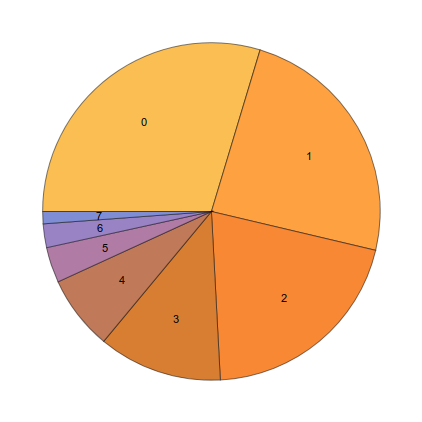
\includegraphics[width=0.5\textwidth]{other/args_stat.png}
\caption{Function arguments statistics}
\end{figure}

This is heavily dependent on programming style and may be very different for other software products.

}
\DE{\section{Statistiken von Funktionsargumenten}
\label{args_stat}

Ich war immer sehr daran interessiert welches die durchschnittliche Anzahl von
Argumenten der einzelnen Funktionen ist.

\index{UNIX!grep}
Dazu wurden viele Windows 7 32-Bit-DLLs analysiert
(crypt32.dll, mfc71.dll, msvcr100.dll, shell32.dll, user32.dll, d3d11.dll, mshtml.dll,
msxml6.dll, sqlncli11.dll, wininet.dll, mfc120.dll, msvbvm60.dll, ole32.dll, themeui.dll,
wmp.dll), da diese die stdcall-Konvention nutzen, was es einfach macht das Ergebnis des
Disassemblers mit grep nach \INS{RETN X} zu durchsuchen.

\begin{itemize}
\item keine Argumente: ~29\%
\item 1 Argument: ~23\%
\item 2 Argumente: ~20\%
\item 3 Argumente: ~11\%
\item 4 Argumente: ~7\%
\item 5 Argumente: ~3\%
\item 6 Argumente: ~2\%
\item 7 Argumente: ~1\%
\end{itemize}

\begin{figure}[H]
\centering
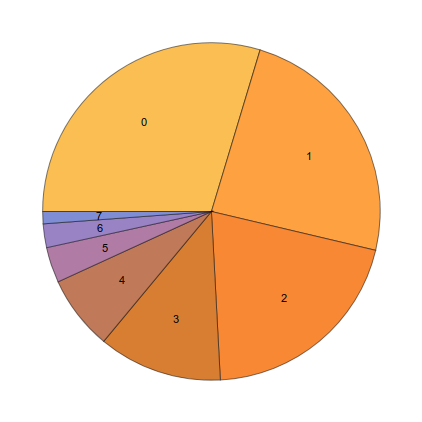
\includegraphics[width=0.5\textwidth]{other/args_stat.png}
\caption{Statistiken von Funktionsargumenten}
\end{figure}

Das Ergebnis ist stark vom Programmierstil abhängig und kann bei anderen Programmen
deutlich anders ausfallen.
}

\EN{\section{Compiler intrinsic}
\myindex{Compiler intrinsic}
\label{sec:compiler_intrinsic}

\myindex{x86!\Instructions!ROL}
\myindex{x86!\Instructions!ROR}

A function specific to a compiler which is not an usual library function.
The compiler generates a specific machine code instead of a call to it.
It is often a pseudofunction for specific \ac{CPU} instruction. \\
\\
For example, there are no cyclic shift operations in \CCpp languages, but they are present in most \ac{CPU}s.
For programmer's convenience, at least MSVC has pseudofunctions
\IT{\_rotl()} and \IT{\_rotr()}\FNMSDNROTxURL{}
which are translated by the compiler directly to the ROL/ROR x86 instructions. \\
\\
Another example are functions to generate SSE-instructions right in the code.

Full list of MSVC intrinsics: \href{http://go.yurichev.com/17254}{MSDN}.

}
\RU{\section{Compiler intrinsic}
\myindex{Compiler intrinsic}
\label{sec:compiler_intrinsic}

\myindex{x86!\Instructions!ROL}
\myindex{x86!\Instructions!ROR}
Специфичная для компилятора функция не являющаяся обычной библиотечной функцией.
Компилятор вместо её вызова генерирует определенный машинный код.
Нередко, это псевдофункции для определенной инструкции \ac{CPU}. \\
\\
Например, в языках \CCpp нет операции циклического сдвига, а во многих \ac{CPU} она есть.
Чтобы программисту были доступны эти инструкции, в MSVC есть псевдофункции 
\IT{\_rotl()} and \IT{\_rotr()}\FNMSDNROTxURL{},
которые компилятором напрямую транслируются в x86-инструкции \TT{ROL}/\TT{ROR}. \\
\\
Еще один пример это функции позволяющие генерировать SSE-инструкции прямо в коде.

Полный список intrinsics от MSVC: \href{http://go.yurichev.com/17254}{MSDN}.

}
\DE{\section{Intrinsische Compiler-Funktionen}
\myindex{Compiler intrinsic}
\label{sec:compiler_intrinsic}

\myindex{x86!\Instructions!ROL}
\myindex{x86!\Instructions!ROR}

Dabei handelt es sich um spezielle Funktionen eines Compilers, die nicht in der
Standard-Bibliothek enthalten sind.
Der Compiler generiert einen spezifischen Maschinencode anstatt ihn aufzurufen.
Dies ist häufig eine Pseudofunktion für eine spezielle \ac{CPU}-Anweisung.

Beispielsweise gibt es keine zyklische Schiebe-Anweisungen in \CCpp -Sprachen,
in den meisten \ac{CPU}s sind sie jedoch vorhanden.
Um dem Programmierer das Leben einfacher zu machen hat zumindest MSVC die
Pseudofunktionen \IT{\_rotl()} und \IT{\_rotr()}\FNMSDNROTxURL{} welche vom
Compiler direkt in die ROL/ROR x86-Anweisungen übersetzt werden.

Ein anderes Beispiel sind Funktionen die SSE-Anweisungen direkt im Code umwandeln.

Eine vollständige Liste von intrinsischen Funktionen in MSVC ist hier zu finden:
\href{http://go.yurichev.com/17254}{MSDN}.
}

\EN{\section{Compiler's anomalies}
\label{anomaly:Intel}
\myindex{\CompilerAnomaly}

\subsection{\oracle 11.2 and Intel C++ 10.1}

\myindex{Intel C++}
\myindex{\oracle}
\myindex{x86!\Instructions!JZ}

Intel C++ 10.1, which was used for \oracle 11.2 Linux86 compilation, may emit two \JZ in row,
and there are no references to the second \JZ. The second \JZ is thus meaningless.

\begin{lstlisting}[caption=kdli.o from libserver11.a,style=customasmx86]
.text:08114CF1                   loc_8114CF1: ; CODE XREF: __PGOSF539_kdlimemSer+89A
.text:08114CF1                                ; __PGOSF539_kdlimemSer+3994
.text:08114CF1 8B 45 08              mov     eax, [ebp+arg_0]
.text:08114CF4 0F B6 50 14           movzx   edx, byte ptr [eax+14h]
.text:08114CF8 F6 C2 01              test    dl, 1
.text:08114CFB 0F 85 17 08 00 00     jnz     loc_8115518
.text:08114D01 85 C9                 test    ecx, ecx
.text:08114D03 0F 84 8A 00 00 00     jz      loc_8114D93
.text:08114D09 0F 84 09 08 00 00     jz      loc_8115518
.text:08114D0F 8B 53 08              mov     edx, [ebx+8]
.text:08114D12 89 55 FC              mov     [ebp+var_4], edx
.text:08114D15 31 C0                 xor     eax, eax
.text:08114D17 89 45 F4              mov     [ebp+var_C], eax
.text:08114D1A 50                    push    eax
.text:08114D1B 52                    push    edx
.text:08114D1C E8 03 54 00 00        call    len2nbytes
.text:08114D21 83 C4 08              add     esp, 8
\end{lstlisting}

\begin{lstlisting}[caption=from the same code,style=customasmx86]
.text:0811A2A5                   loc_811A2A5: ; CODE XREF: kdliSerLengths+11C
.text:0811A2A5                                ; kdliSerLengths+1C1
.text:0811A2A5 8B 7D 08              mov     edi, [ebp+arg_0]
.text:0811A2A8 8B 7F 10              mov     edi, [edi+10h]
.text:0811A2AB 0F B6 57 14           movzx   edx, byte ptr [edi+14h]
.text:0811A2AF F6 C2 01              test    dl, 1
.text:0811A2B2 75 3E                 jnz     short loc_811A2F2
.text:0811A2B4 83 E0 01              and     eax, 1
.text:0811A2B7 74 1F                 jz      short loc_811A2D8
.text:0811A2B9 74 37                 jz      short loc_811A2F2
.text:0811A2BB 6A 00                 push    0
.text:0811A2BD FF 71 08              push    dword ptr [ecx+8]
.text:0811A2C0 E8 5F FE FF FF        call    len2nbytes
\end{lstlisting}

It is supposedly a code generator bug that was not found by tests, because 
resulting code works correctly anyway.

% TODO to be translated ...
\input{other/anomaly2_EN}

\subsection{Summary}

Other compiler anomalies here in this book: 
\myref{anomaly:LLVM}, \myref{loops_iterators_loop_anomaly}, \myref{Keil_anomaly},
\myref{MSVC2013_anomaly},
\myref{MSVC_double_JMP_anomaly},
\myref{MSVC2012_anomaly}.

Such cases are demonstrated here in this book, to show that such compilers errors are possible and sometimes
one should not to rack one's brain while thinking why did the compiler generate such strange code.

}
\RU{\section{Аномалии компиляторов}
\label{anomaly:Intel}
\myindex{\CompilerAnomaly}

\subsection{\oracle 11.2 and Intel C++ 10.1}

\myindex{Intel C++}
\myindex{\oracle}
\myindex{x86!\Instructions!JZ}

Intel C++ 10.1 которым скомпилирован \oracle 11.2 Linux86, может сгенерировать два \JZ идущих подряд, 
причем на второй \JZ нет ссылки ниоткуда. Второй \JZ таким образом, не имеет никакого смысла.

\begin{lstlisting}[caption=kdli.o из libserver11.a,style=customasmx86]
.text:08114CF1                   loc_8114CF1: ; CODE XREF: __PGOSF539_kdlimemSer+89A
.text:08114CF1                                ; __PGOSF539_kdlimemSer+3994
.text:08114CF1 8B 45 08              mov     eax, [ebp+arg_0]
.text:08114CF4 0F B6 50 14           movzx   edx, byte ptr [eax+14h]
.text:08114CF8 F6 C2 01              test    dl, 1
.text:08114CFB 0F 85 17 08 00 00     jnz     loc_8115518
.text:08114D01 85 C9                 test    ecx, ecx
.text:08114D03 0F 84 8A 00 00 00     jz      loc_8114D93
.text:08114D09 0F 84 09 08 00 00     jz      loc_8115518
.text:08114D0F 8B 53 08              mov     edx, [ebx+8]
.text:08114D12 89 55 FC              mov     [ebp+var_4], edx
.text:08114D15 31 C0                 xor     eax, eax
.text:08114D17 89 45 F4              mov     [ebp+var_C], eax
.text:08114D1A 50                    push    eax
.text:08114D1B 52                    push    edx
.text:08114D1C E8 03 54 00 00        call    len2nbytes
.text:08114D21 83 C4 08              add     esp, 8
\end{lstlisting}

\begin{lstlisting}[caption=оттуда же,style=customasmx86]
.text:0811A2A5                   loc_811A2A5: ; CODE XREF: kdliSerLengths+11C
.text:0811A2A5                                ; kdliSerLengths+1C1
.text:0811A2A5 8B 7D 08              mov     edi, [ebp+arg_0]
.text:0811A2A8 8B 7F 10              mov     edi, [edi+10h]
.text:0811A2AB 0F B6 57 14           movzx   edx, byte ptr [edi+14h]
.text:0811A2AF F6 C2 01              test    dl, 1
.text:0811A2B2 75 3E                 jnz     short loc_811A2F2
.text:0811A2B4 83 E0 01              and     eax, 1
.text:0811A2B7 74 1F                 jz      short loc_811A2D8
.text:0811A2B9 74 37                 jz      short loc_811A2F2
.text:0811A2BB 6A 00                 push    0
.text:0811A2BD FF 71 08              push    dword ptr [ecx+8]
.text:0811A2C0 E8 5F FE FF FF        call    len2nbytes
\end{lstlisting}

Возможно, это ошибка его кодегенератора, не выявленная тестами 
(ведь результирующий код и так работает нормально).

\subsection{Итог}

Еще подобные аномалии компиляторов в этой книге: 
\myref{anomaly:LLVM}, \myref{loops_iterators_loop_anomaly}, \myref{Keil_anomaly},
\myref{MSVC2013_anomaly},
\myref{MSVC_double_JMP_anomaly},
\myref{MSVC2012_anomaly}.

В этой книге здесь приводятся подобные случаи для того, чтобы легче было понимать, 
что подобные ошибки компиляторов 
все же имеют место быть, и не следует ломать голову над тем, почему он сгенерировал такой странный код.%

}
\DE{\section{Compiler Anomalien}
\label{anomaly:Intel}
\myindex{\CompilerAnomaly}

\subsection{\oracle 11.2 und Intel C++ 10.1}

\myindex{Intel C++}
\myindex{\oracle}
\myindex{x86!\Instructions!JZ}

Der Intel C++ 10.1-Compiler, der für \oracle 11.2 für Linux 86 genutzt wurde, kann
zwei \JZ in einer Reihe ausgeben. Es gibt keine Referenz zum zweiten \JZ. Das zweite
ist also ohne Bedeutung.

\begin{lstlisting}[caption=kdli.o from libserver11.a,style=customasmx86]
.text:08114CF1                   loc_8114CF1: ; CODE XREF: __PGOSF539_kdlimemSer+89A
.text:08114CF1                                ; __PGOSF539_kdlimemSer+3994
.text:08114CF1 8B 45 08              mov     eax, [ebp+arg_0]
.text:08114CF4 0F B6 50 14           movzx   edx, byte ptr [eax+14h]
.text:08114CF8 F6 C2 01              test    dl, 1
.text:08114CFB 0F 85 17 08 00 00     jnz     loc_8115518
.text:08114D01 85 C9                 test    ecx, ecx
.text:08114D03 0F 84 8A 00 00 00     jz      loc_8114D93
.text:08114D09 0F 84 09 08 00 00     jz      loc_8115518
.text:08114D0F 8B 53 08              mov     edx, [ebx+8]
.text:08114D12 89 55 FC              mov     [ebp+var_4], edx
.text:08114D15 31 C0                 xor     eax, eax
.text:08114D17 89 45 F4              mov     [ebp+var_C], eax
.text:08114D1A 50                    push    eax
.text:08114D1B 52                    push    edx
.text:08114D1C E8 03 54 00 00        call    len2nbytes
.text:08114D21 83 C4 08              add     esp, 8
\end{lstlisting}

\begin{lstlisting}[caption=from the same code,style=customasmx86]
.text:0811A2A5                   loc_811A2A5: ; CODE XREF: kdliSerLengths+11C
.text:0811A2A5                                ; kdliSerLengths+1C1
.text:0811A2A5 8B 7D 08              mov     edi, [ebp+arg_0]
.text:0811A2A8 8B 7F 10              mov     edi, [edi+10h]
.text:0811A2AB 0F B6 57 14           movzx   edx, byte ptr [edi+14h]
.text:0811A2AF F6 C2 01              test    dl, 1
.text:0811A2B2 75 3E                 jnz     short loc_811A2F2
.text:0811A2B4 83 E0 01              and     eax, 1
.text:0811A2B7 74 1F                 jz      short loc_811A2D8
.text:0811A2B9 74 37                 jz      short loc_811A2F2
.text:0811A2BB 6A 00                 push    0
.text:0811A2BD FF 71 08              push    dword ptr [ecx+8]
.text:0811A2C0 E8 5F FE FF FF        call    len2nbytes
\end{lstlisting}

Dies ist vermutlich ein Fehler im Codegenerator der während der Tests nicht
gefunden wurde. Der resultierende Code funktioniert trotzdem.

% TODO to be translated ...
\input{other/anomaly2_DE}

\subsection{Zusammenfassung}

Andere Compiler-Anomalien in diesem Buch:
\myref{anomaly:LLVM}, \myref{loops_iterators_loop_anomaly}, \myref{Keil_anomaly},
\myref{MSVC2013_anomaly},
\myref{MSVC_double_JMP_anomaly},
\myref{MSVC2012_anomaly}.

Diese Beispiele werden in diesem Buch gezeigt, um zu verdeutlichen, das solche Fehler
in den Compilern möglich sind und es gelegentlich keinen Sinn ergibt sich den Kopf
darüber zu zerbrechen warum der Compiler diesen \q{seltsamen} Code erzeugte.
}

\EN{\section{Itanium}
\label{itanium}
\myindex{Itanium}

Although almost failed, Intel Itanium (\ac{IA64}) is a very interesting architecture.

While \ac{OOE} CPUs decides how to rearrange their instructions and execute them in parallel,
\ac{EPIC} was an attempt to shift these decisions to the compiler:
to let it group the instructions at the compile stage.

This resulted in notoriously complex compilers.

Here is one sample of \ac{IA64} code: simple cryptographic algorithm from the Linux kernel:

\lstinputlisting[caption=Linux kernel 3.2.0.4,style=customc]{other/itanium/tea_from_linux.c}

Here is how it was compiled:

\lstinputlisting[caption=Linux Kernel 3.2.0.4 for Itanium 2 (McKinley)]{other/itanium/ia64_linux_3.2.0.4_mckinley.lst}

First of all, all \ac{IA64} instructions are grouped into 3-instruction bundles.

Each bundle has a size of 16 bytes (128 bits) and consists of template code (5 bits) + 3 instructions (41 bits for each).

\IDA shows the bundles as 6+6+4 bytes~---you can easily spot the pattern.

All 3 instructions from each bundle usually executes simultaneously, unless one of instructions has a \q{stop bit}.

Supposedly, Intel and HP engineers gathered statistics on most frequent instruction patterns and decided to bring
bundle types (\ac{AKA} \q{templates}): a bundle code defines the instruction types in the bundle.
There are 12 of them.

For example, the zeroth bundle type is \TT{MII}, which implies 
the first instruction is Memory (load or store), the second and third ones are I (integer instructions).

Another example is the bundle of type 0x1d: \TT{MFB}:
the first instruction is Memory (load or store), the second one is Float 
(\ac{FPU} instruction), and the third is Branch (branch instruction).

If the compiler cannot pick a suitable instruction for the relevant bundle slot, it may insert a \ac{NOP}:
you can see here the
\TT{nop.i} instructions (\ac{NOP} at the place where the integer instruction might be) or \TT{nop.m} 
(a memory instruction might be at this slot).

\ac{NOP}s are inserted automatically when one uses assembly language manually.

And that is not all. Bundles are also grouped.

Each bundle may have a \q{stop bit},
so all the consecutive bundles with a terminating bundle which has the \q{stop bit} 
can be executed simultaneously.

In practice, Itanium 2 can execute 2 bundles at once, resulting in the execution of 6 instructions at once.

So all instructions inside a bundle and a bundle group cannot interfere with each other 
(i.e., must not have data hazards).

If they do, the results are to be undefined.

Each stop bit is marked in assembly language as two semicolons (\TT{;;}) after the instruction.

So, the instructions at [90-ac] may be executed simultaneously:
they do not interfere. The next group is [b0-cc].

We also see a stop bit at 10c.
The next instruction at 110 has a stop bit too.

This implies that these instructions must be executed isolated from all others (as in \ac{CISC}).

Indeed: the next instruction at 110 uses the result from the previous one (the value in register r26),
so they cannot be executed at the same time.

Apparently, the compiler was not able to find a better way to parallelize the instructions,
in other words, to load \ac{CPU} as much as possible, hence too much stop bits and \ac{NOP}s.

Manual assembly programming is a tedious job as well: the programmer has to group the instructions manually.

The programmer is still able to add stop bits to each instructions, but this will degrade
the performance that Itanium was made for.

An interesting examples of manual \ac{IA64} assembly code can be found in the Linux kernel's sources:

\url{http://go.yurichev.com/17322}.

Another introductory paper on Itanium assembly:
[Mike Burrell, \IT{Writing Efficient Itanium 2 Assembly Code} (2010)]\footnote{\AlsoAvailableAs \url{http://yurichev.com/mirrors/RE/itanium.pdf}},
[papasutra of haquebright, \IT{WRITING SHELLCODE FOR IA-64} (2001)]\footnote{\AlsoAvailableAs \url{http://phrack.org/issues/57/5.html}}.

Another very interesting Itanium feature is the \IT{speculative execution} and the NaT (\q{not a thing}) bit,
somewhat resembling \gls{NaN} numbers: \\
\href{http://go.yurichev.com/17323}{MSDN}.

}
\RU{\section{Itanium}
\label{itanium}
\myindex{Itanium}
Еще одна очень интересная архитектура (хотя и почти провальная) это Intel Itanium (\ac{IA64}).
Другие \ac{OOE}-процессоры сами решают, как переставлять инструкции и исполнять их параллельно,
\ac{EPIC} это была попытка сдвинуть эти решения на компилятор: дать ему возможность самому 
группировать инструкции во время компиляции.

Это вылилось в очень сложные компиляторы.

Вот один пример \ac{IA64}-кода: простой криптоалгоритм из ядра Linux:

\lstinputlisting[caption=Linux kernel 3.2.0.4,style=customc]{other/itanium/tea_from_linux.c}

И вот как он был скомпилирован:

\lstinputlisting[caption=Linux Kernel 3.2.0.4 для Itanium 2 (McKinley)]{other/itanium/ia64_linux_3.2.0.4_mckinley.lst}

Прежде всего, все инструкции \ac{IA64} сгруппированы в пачки (bundle) из трех инструкций.
Каждая пачка имеет размер 16 байт (128 бит) и состоит из template-кода (5 бит) и трех инструкций (41 бит на каждую).

\IDA показывает пачки как 6+6+4 байт --- вы можете легко заметить эту повторяющуюся структуру.

Все 3 инструкции каждой пачки обычно исполняются одновременно, если только у какой-то инструкции
нет \q{стоп-бита}.

Может быть, инженеры Intel и HP собрали статистику наиболее встречающихся шаблонных сочетаний
инструкций и решили ввести типы пачек (\ac{AKA} \q{templates}): код пачки определяет типы инструкций
в пачке.
Их всего 12.
Например, нулевой тип это \TT{MII}, что означает: первая инструкция это Memory (загрузка
или запись в память), вторая и третья это I (инструкция, работающая с целочисленными значениями).

Еще один пример, тип 0x1d: \TT{MFB}: первая инструкция это Memory (загрузка или запись
в память), вторая это Float (инструкция, работающая с \ac{FPU}), третья это Branch (инструкция
перехода).

Если компилятор не может подобрать подходящую инструкцию в соответствующее место пачки,
он может вставить \ac{NOP}:
вы можете здесь увидеть инструкции \TT{nop.i} (\ac{NOP} на том месте где должна была бы находиться
целочисленная инструкция) или \TT{nop.m} (инструкция обращения к памяти должна была находиться
здесь).

Если вручную писать на ассемблере, \ac{NOP}-ы могут вставляться автоматически.

И это еще не все. Пачки тоже могут быть объединены в группы.
Каждая пачка может иметь \q{стоп-бит}, так что все следующие друг за другом пачки вплоть до той,
что имеет стоп-бит, могут быть исполнены одновременно.
На практике, Itanium 2 может исполнять 2 пачки одновременно, таким образом, исполнять
6 инструкций одновременно.

Так что все инструкции внутри пачки и группы не могут мешать друг другу (т.е. не должны
иметь data hazard-ов).
А если это так, то результаты будут непредсказуемые.

На ассемблере, каждый стоп-бит маркируется как две точки с запятой (\TT{;;}) после инструкции.

Так, инструкции на [90-ac] могут быть исполнены одновременно: они не мешают друг другу. Следующая группа: [b0-cc].

Мы также видим стоп-бит на 10c.
Следующая инструкция на 110 также имеет стоп-бит.
Это значит, что эти инструкции должны исполняться изолированно от всех остальных (как в \ac{CISC}).
Действительно: следующая инструкция на 110 использует результат, полученный от предыдущей (значение
в регистре r26), так что они не могут исполняться одновременно.
Должно быть, компилятор не смог найти лучший способ распараллелить инструкции, или, иными
словами, загрузить \ac{CPU} насколько это возможно, отсюда так много стоп-битов и \ac{NOP}-ов.
Писать на ассемблере вручную это также очень трудная задача: программист должен группировать
инструкции вручную.

У программиста остается возможность добавлять стоп-биты к каждой инструкции, но это
сведет на нет всю мощность Itanium, ради которой он создавался.

Интересные примеры написания \ac{IA64}-кода вручную можно найти в исходниках ядра Linux:

\url{http://go.yurichev.com/17322}.

Еще пара вводных статей об ассемблере Itanium:
[Mike Burrell, \IT{Writing Efficient Itanium 2 Assembly Code} (2010)]\footnote{\AlsoAvailableAs \url{http://yurichev.com/mirrors/RE/itanium.pdf}},
[papasutra of haquebright, \IT{WRITING SHELLCODE FOR IA-64} (2001)]\footnote{\AlsoAvailableAs \url{http://phrack.org/issues/57/5.html}}.

Еще одна интересная особенность Itanium это \IT{speculative execution} (исполнение инструкций
заранее, когда еще не известно, нужно ли это) и бит NaT (\q{not a thing}), отдаленно напоминающий
\gls{NaN}-числа: \\
\href{http://go.yurichev.com/17323}{MSDN}.

}
\DE{\section{Itanium}
\label{itanium}
\myindex{Itanium}

Auch wenn fast gescheitert, ist der Intel Itanium (\ac{IA64}) eine sehr interessante
Architektur.

Während \ac{OOE}-CPUs entscheiden wie die Anweisungen neu organisiert werden und
diese parallel ausführen, war \ac{EPIC} ein Versuch diese Entscheidung dem Compiler
zu überlassen: das Gruppieren der Anweisungen soll während des Kompilierens erfolgen.

Dies führte zu einer berüchtigten Komplexität der Compiler.

Hier ist ein Beispiel von \ac{IA64}-Code, ein einfacher kryptografischer Algorithmus
aus dem Linux-Kernel:

\lstinputlisting[caption=Linux kernel 3.2.0.4,style=customc]{other/itanium/tea_from_linux.c}

Nachfolgend das Ergebnis des Compilers:

\lstinputlisting[caption=Linux Kernel 3.2.0.4 for Itanium 2 (McKinley)]{other/itanium/ia64_linux_3.2.0.4_mckinley.lst}

Zunächst sind alle \ac{IA64}-Anweisungen in Pakete von 3 Anweisungen zusammengefasst.

Jedes Paket hat eine Größe von 16 Byte (128 Bit) und besteht aus Template-Code
(5 Bit) und drei Anweisungen (je 41 Bit).

\IDA zeigt die Pakete als 6+6+4 Byte, das Muster ist leicht zu erkennen.

Alle drei Anweisungen von jedem Paket wird in der Regel gleichzeitig ausgeführt,
außer eine der Anweisungen enthält ein \q{Stop-Bit}.

Vermutlich haben die Intel- und HP-Ingenieure Statistiken über die am meisten verwendeten
Anweisungsmuster erhoben und entschieden die Pakettypen zu erstellen (\ac{AKA} \q{Templates}): 
ein Paket-Code definiert den Anweisungstyp im Paket.
Es existieren 12 von ihnen.

Beispielsweise ist der nullte Pakettyp \TT{MII}, was impliziert, dass die erste
Anweisung Speicher (Lesen oder Schreiben) ist und die zweite und dritte jeweils
eine Integer-Anweisung ist.

Ein weiteres Beispiel ist das Paket vom Typ 0x1d: \TT{MFB}:
die erste Anweisung ist betrifft wieder den Speicher (Lesen oder Schreiben), die
zweite eine Fließkomma (\ac{FPU} Anweisung) und die dritte ein Springbefehl.

Wenn der Compiler keine passende Anweisung für den entsprechenden Paketplatz finden
kann, ist es möglich, dass er ein \ac{NOP} einfügt: man kann hier die \TT{nop.i}-Anweisung
(\ac{NOP} anstelle einer Integer-Anweisung) oder \TT{nop.m} (anstelle einer Speicheroperation)
sehen .

\ac{NOP}s werden automatisch eingefügt wenn mit Assembler gearbeitet wird.

Dies ist nicht alles: Pakete können ebenfalls grupiert werden.

Jedes Paket kann ein  \q{Stop-Bit} enthalten, so dass alle aufeinander folgenden
Pakete mit einem terminierenden Paket (mit \q{Stop-Bit}) gleichzeitig verarbeitet
werden können.

In der Praxis kann Itanium 2 gleichzeitig zwei Pakete ausführen, was zu sechs
Anweisungen führt.

Also kann keine der Anweisungen innerhalb einer Paket-Gruppe mit einer anderen
interagieren (es kann also nicht zu Datenkonflikten kommen).

Falls sie auftreten können die Ergebnisse undefiniert sein.

Jedes Stop-Bit ist in Assembler mit zwei Semikolons (\TT{;;}) nach de Anweisung markiert.

Die Anweisungen bei [90-ac] können also simultan ausgeführt werden: sie beeinflussen
sich gegenseitig nicht. Die nächste Gruppe ist [b0-cc].

Hier ist auch das Stop-Bit bei 10c zu sehen
Die nächste Anweisung bei 110 hat ebenfalls ein Stop-Bit.

Dies impliziert dass diese Anweisungen von allen anderen getrennt ausgeführt werden
müssen (wie in \ac{CISC}).

Außerdem ist zu sehen, dass die Anweisung nach 110 das Ergebnis der vorangehenden
benutzt (Den Wert im Register r26), dementsprechend können sie nicht gleichzeitig
ausgeführt werden.

Anscheinend war der Compiler nicht in der Lage einen besseren Weg zum Parallelisieren
der Anweisungen zu finden, also die \ac{CPU} so weit wie möglich auszulasten. Daher
die vielen Stop-Bits und \ac{NOP}-Anweisungen.

Manuelle Assembler-Programmierung ist ein mühsamer Job: der Programmierer muss
die Anweisungen selber in Gruppen einteilen.

Der Programmierer ist immer noch in der Lage Stop-Bits zu jeder Anweisung hinzuzufügen,
doch dies wird die Geschwindigkeit heruntersetzen für die Itanium gemacht wurde.

Ein interessantes Beispiel von manuellem Assembler-Code in \ac{IA64} kann im Code
des Linux-Kernels gefunden werden:

\url{http://go.yurichev.com/17322}.

Eine weitere Einführung für den Itanium-Assembler:
[Mike Burrell, \IT{Writing Efficient Itanium 2 Assembly Code} (2010)]\footnote{\AlsoAvailableAs \url{http://yurichev.com/mirrors/RE/itanium.pdf}},
[papasutra of haquebright, \IT{WRITING SHELLCODE FOR IA-64} (2001)]\footnote{\AlsoAvailableAs \url{http://phrack.org/issues/57/5.html}}.

Weitere sehr interessante Itanium-Features sind \IT{speculative execution} und das
NaT (\q{not a thing})-Bit, was in gewisser Weise \gls{NaN}-Zahlen ähnelt:

\href{http://go.yurichev.com/17323}{MSDN}
}

\EN{\section{8086 memory model}
\myindex{Intel!8086!Memory model}
\myindex{MS-DOS}
\label{8086_memory_model}

When dealing with 16-bit programs for MS-DOS or Win16
(\myref{dongle_16bit_dos} or \myref{win16_near_far_pointers}),
we can see that the pointers consist of two 16-bit values.
What do they mean? Oh yes, that is another weird MS-DOS and 8086 artifact.

8086/8088 was a 16-bit CPU, but was able to address 20-bit address in RAM 
(thus being able to access 1MB of external memory).

The external memory address space was divided between \ac{RAM} (640KB max),
\ac{ROM}, windows for video memory, EMS cards, \etc{}.

Let's also recall that 8086/8088 was in fact an inheritor of the 8-bit 8080 CPU.

The 8080 has a 16-bit memory space, i.e., it was able to address only 64KB.

And probably because of reason of old software porting\footnote{The author is not 100\% sure here},
8086 can support many 64KB windows simultaneously, placed
within the 1MB address space.

This is some kind of a toy-level virtualization.
\myindex{x86!\Registers!CS}
\myindex{x86!\Registers!DS}
\myindex{x86!\Registers!ES}
\myindex{x86!\Registers!SS}

All 8086 registers are 16-bit, so to address more, special segment registers (CS, DS, ES, SS) were
introduced.

Each 20-bit pointer is calculated using the values from a segment register and 
an address register pair (e.g. DS:BX) as follows:

\begin{center}
$real\_address = (segment\_register \ll 4) + address\_register$
\end{center}

For example, the graphics (\ac{EGA}, \ac{VGA}) video \ac{RAM} window on old IBM PC-compatibles 
has a size of 64KB.

To access it, a value of 0xA000 has to be stored in one of the segment registers, e.g. into DS.

Then DS:0 will address the first byte of video \ac{RAM} and DS:0xFFFF ~--- the last byte of RAM.

The real address on the 20-bit address bus, however, will range from 0xA0000 to 0xAFFFF.

The program may contain hard-coded addresses like 0x1234, but the \ac{OS} may need to load the program at arbitrary
addresses, so it recalculates the segment register values in a way that the program does not have to care 
where it's placed in the RAM.

So, any pointer in the old MS-DOS environment in fact consisted of the segment address and the address inside
segment, i.e., two 16-bit values. 20-bit was enough for that, though, but we needed to recalculate
the addresses very often: passing more information on the stack seemed a better space/convenience balance.

By the way, because of all this it was not possible to allocate a memory block larger than 64KB.

\myindex{Intel!80286}
\myindex{Intel!80386}

The segment registers were reused at 80286 as selectors, serving a different function.

\myindex{MS-DOS!DOS extenders}

When the 80386 CPU and computers with bigger \ac{RAM} were introduced,
MS-DOS was still popular, so the DOS extenders emerged: these were in fact
a step toward a \q{serious} \ac{OS},
switching the CPU in protected mode and providing much better memory \ac{API}s for the programs 
which still needed to run under MS-DOS.

Widely popular examples include DOS/4GW (the DOOM video game was compiled for it), Phar Lap, PMODE.
\par
\myindex{Windows!Windows 3.x}
\myindex{Windows!Win32}

By the way, the same way of addressing memory was used in the 16-bit line of Windows 3.x, before Win32.

}
\RU{\section{Модель памяти в 8086}
\myindex{Intel!8086!Модель памяти}
\myindex{MS-DOS}
\label{8086_memory_model}

Разбирая 16-битные программы для MS-DOS или Win16
(\myref{dongle_16bit_dos} или \myref{win16_near_far_pointers}),
мы можем увидеть, что указатель состоит из двух 16-битных значений.
Что это означает? О да, еще один дивный артефакт MS-DOS и 8086.

8086/8088 был 16-битным процессором, но мог адресовать 20-битное адресное
пространство (таким образом мог адресовать 1MB внешней памяти).
Внешняя адресное пространство было разделено между \ac{RAM} (максимум 640KB),
\ac{ROM}, окна для видеопамяти, EMS-карт, \etc{}.

Припомним также что 8086/8088 был на самом деле наследником 8-битного процессора 8080.
Процессор 8080 имел 16-битное адресное пространство, т.е. мог адресовать только 64KB.
И возможно в расчете на портирование старого ПО\footnote{Автор не уверен на 100\% здесь},
8086 может поддерживать 64-килобайтные
окна, одновременно много таких, расположенных внутри одномегабайтного адресного пространства.
Это, в каком-то смысле, игрушечная виртуализация.
\myindex{x86!\Registers!CS}
\myindex{x86!\Registers!DS}
\myindex{x86!\Registers!ES}
\myindex{x86!\Registers!SS}
Все регистры 8086 16-битные, так что, чтобы адресовать больше, специальные сегментные
регистры (CS, DS, ES, SS) были введены.
Каждый 20-битный указатель вычисляется, используя значения из пары состоящей из сегментного регистра
и адресного регистра (например DS:BX) вот так:

\begin{center}
$real\_address = (segment\_register \ll 4) + address\_register$
\end{center}

Например, окно памяти для графики (\ac{EGA}, \ac{VGA}) на старых IBM PC-совместимых компьютерах
имело размер 64KB.

Для доступа к нему, значение 0xA000 должно быть записано в один из сегментных регистров,
например, в DS.

Тогда DS:0 будет адресовать самый первый байт видеопамяти, а DS:0xFFFF ~--- самый последний байт.

А реальный адрес на 20-битной адресной шине, на самом деле будет от 0xA0000 до 0xAFFFF.

Программа может содержать жесткопривязанные адреса вроде 0x1234, но \ac{OS} может иметь необходимость
загрузить программу по другим адресам, так что она пересчитает значения для сегментных регистров так,
что программа будет нормально работать, не обращая внимания на то,
в каком месте памяти она была расположена.

Так что, любой указатель в окружении старой MS-DOS на самом деле состоял из адреса сегмента
и адреса внутри сегмента, т.е. из двух 16-битных значений. 20-битного значения было бы достаточно для
этого, хотя, тогда пришлось бы вычислять адреса слишком часто: так что передача большего количества
информации в стеке ~--- это более хороший баланс между экономией места и удобством.

Кстати, из-за всего этого, не было возможным выделить блок памяти больше чем 64KB.

\myindex{Intel!80286}
\myindex{Intel!80386}
В 80286 сегментные регистры получили новую роль селекторов, имеющих немного другую функцию.

\myindex{MS-DOS!DOS extenders}
Когда появился процессор 80386 и компьютеры с большей памятью,
MS-DOS была всё еще популярна, так что появились DOS-экстендеры: на самом деле это уже был шаг
к \q{серьезным} \ac{OS}, они переключали \ac{CPU} в защищенный режим и предлагали куда лучшее \ac{API} для
программ, которые всё еще предполагалось запускать в MS-DOS.

Широко известные примеры это DOS/4GW (игра DOOM была скомпилирована под него), Phar Lap, PMODE.

\par
\myindex{Windows!Windows 3.x}
\myindex{Windows!Win32}
Кстати, точно такой же способ адресации памяти был и в 16-битной линейке Windows 3.x, перед Win32.

}
\DE{\section{8086-Speichermodell}
\myindex{Intel!8086!Memory model}
\myindex{MS-DOS}
\label{8086_memory_model}

Wenn es um 16-Bit-Programme für MS-DOS oder Win16 geht (\myref{dongle_16bit_dos}
oder \myref{win16_near_far_pointers}), kann man sehen, dass die Zeiger aus zwei
16-Bit-Werten bestehen.
Was bedeutet das? Ja, das ist wieder ein weiteres sonderbares Artefakt von MS-DOS
und 8086.

8086/8088 war eine 16-Bit-CPU, war aber in der Lage 20-Bit-Adressen im RAM anzusprechen
(und somit externen Speicher bis 1MB zu adressieren).

Der Adressbereich für externen Speicher ist aufgeteilt zwischen \ac{RAM} (maximal 640KB),
\ac{ROM}, Fenster für Videospeicher, EMS-Karten, \etc{}.

Erinnern wir uns auch nochmal daran, dass der 8086/8088 der Nachfolger der 8-Bit-CPU
8080 war.

Der 8080 hat einen 16-Bit-Adressspeicher, kann also lediglich 64KB Speicher adressieren.

Möglicherweise aus Gründen der Portierung alter Software\footnote{Der Autor ist sich hier jedoch nicht 100\% sicher.},
kann der 8086 viele 64KB-Fenster gleichzeitig unterstützen, die sich im 1MB-Adressbereich
befinden.

Dies ist eine Art Top-Level-Virtualisierung.
\myindex{x86!\Registers!CS}
\myindex{x86!\Registers!DS}
\myindex{x86!\Registers!ES}
\myindex{x86!\Registers!SS}

Alle 8086-Register sind 16-Bit breit. Um einen größeren Bereich adressieren zu können,
wurden spezielle Segment-Register (CS, DS, ES, SS)  eingeführt.

Jeder 20-Bit-Zeiger wird aus den Werten eines Segment-Registers und einem
Adressregister-Paar (z.B. DS:BX) berechnet.

\begin{center}
$reale\_adresse = (segment\_register \ll 4) + adress\_register$
\end{center}

Zum Beispiel: das Grafik-Video-Speicher-Fenster (\ac{EGA}, \ac{VGA}) auf alten zu
IBM PC kompatiblen Rechnern hat eine Größe von 64KB.

Um darauf zuzugreifen muss der Wert 0xA000 in eines der Segment-Register geschrieben
werden, zum Beispiel in DS.

Anschließend wird DS:0 das erste Byte des Video-RAM und DS:0xFFFF das letzte
Byte adressieren.

Die echte Adresse auf dem 20-Bit-Adressbus ist in dem Bereich zwischen 0xA0000
und 0xAFFFF.

Das Programm kann hart-kodierte Adressen wie 0x1234 beinhalten, das \ac{OS} lädt
das Programm aber bei Bedarf an eine beliebige Adresse. Dazu werden die Segment-Registerwerte
derart neu berechnet, dass das Programm sich nicht darum kümmern muss an welcher
Stelle im RAM es sich befindet.

Jeder Zeiger in der alten MS-DOS-Umgebung besteht aus der Segmentadresse und der
Adresse innerhalb des Segment, also zwei 16-Bit-Werten. 20 Bit sind hierfür genug,
allerdings muss die Adresse recht oft neu berechnet werden. Mehr Informationen auf
dem Stack zu übergeben schien eine bessere Speicher- / Komfort-Balance zu haben.

Übrigens: aufgrund all der vorherigen Überlegungen war es nicht mögliche Speicherblöcke
zu allozieren die größer 64KB waren.

\myindex{Intel!80286}
\myindex{Intel!80386}

Die Segmentregister wurde beim 80286 als \q{Selektoren} wieder genutzt, jedoch mit
einer anderen Funktion.

\myindex{MS-DOS!DOS extenders}

Als die 80386-CPU mit größerem \ac{RAM} eingeführt wurde, war MS-DOS immer noch
weit verbreite, so das die DOS-Extender auftraten. Diese waren eigentlich ein
Schritt zu einem \q{seriösen} \ac{OS} indem die CPU in den Protected Mode geschaltet
wurde und sehr viel bessere Speicher-\ac{API}s für die Programme angeboten wurden,
die noch unter MS-DOS liefen.

Sehr populäre Beispiele waren DOS/4GW (das Spiel DOOM wurde hierfür kompiliert),
Phar Lap und PMODE.
\par
\myindex{Windows!Windows 3.x}
\myindex{Windows!Win32}

Übrigens wurde das gleiche Adressierungsmodel für Speicher in der 16-Bit-Reihe von
Windows 3.x genutzt, bevor Win32 aufkam.
}

\EN{\section{Basic blocks reordering}

% TODO __builtin_expect in GCC?

\subsection{Profile-guided optimization}
\label{PGO}

\myindex{\oracle}
\myindex{Intel C++}

This optimization method can move some \gls{basic block}s to another section of the executable binary file.

Obviously, there are parts of a function which are executed more frequently (e.g., loop bodies)
and less often (e.g., error reporting code, exception handlers).

The compiler adds instrumentation code into the executable, then the developer runs it with
a lot of tests to collect statistics.

Then the compiler, with the help of the statistics gathered,
prepares final the executable file with all infrequently executed code moved into another section.

As a result, all frequently executed function code is compacted, and that is very important
for execution speed and cache usage.

An example from \oracle code, which was compiled with Intel C++:

\begin{lstlisting}[caption=orageneric11.dll (win32),style=customasmx86]
                public _skgfsync
_skgfsync       proc near

; address 0x6030D86A

                db      66h
                nop
                push    ebp
                mov     ebp, esp
                mov     edx, [ebp+0Ch]
                test    edx, edx
                jz      short loc_6030D884
                mov     eax, [edx+30h]
                test    eax, 400h
                jnz     __VInfreq__skgfsync  ; write to log
continue:
                mov     eax, [ebp+8]
                mov     edx, [ebp+10h]
                mov     dword ptr [eax], 0
                lea     eax, [edx+0Fh]
                and     eax, 0FFFFFFFCh
                mov     ecx, [eax]
                cmp     ecx, 45726963h
                jnz     error                ; exit with error
                mov     esp, ebp
                pop     ebp
                retn
_skgfsync       endp

...

; address 0x60B953F0

__VInfreq__skgfsync:
                mov     eax, [edx]
                test    eax, eax
                jz      continue
                mov     ecx, [ebp+10h]
                push    ecx
                mov     ecx, [ebp+8]
                push    edx
                push    ecx
                push    offset ... ; "skgfsync(se=0x%x, ctx=0x%x, iov=0x%x)\n"
                push    dword ptr [edx+4]
                call    dword ptr [eax] ; write to log
                add     esp, 14h
                jmp     continue

error:
                mov     edx, [ebp+8]
                mov     dword ptr [edx], 69AAh ; 27050 "function called with invalid FIB/IOV structure"
                mov     eax, [eax]
                mov     [edx+4], eax
                mov     dword ptr [edx+8], 0FA4h ; 4004
                mov     esp, ebp
                pop     ebp
                retn
; END OF FUNCTION CHUNK FOR _skgfsync
\end{lstlisting}

The distance of addresses between these two code fragments is almost 9 MB.

All infrequently executed code was placed at the end of the code section of the DLL file,
among all function parts.

This part of the function was marked by the Intel C++ compiler with the \TT{VInfreq} prefix.

Here we see that a part of the function that writes to a log file (presumably in case of error or warning
or something like that) which was probably not executed very often when Oracle's developers gathered 
statistics (if it was executed at all).

The writing to log basic block eventually returns the control flow to the \q{hot} part of the function.

Another \q{infrequent} part is the \gls{basic block} returning error code 27050.

In Linux ELF files, all infrequently executed code is moved by Intel C++ into the separate 
\TT{text.unlikely} section, leaving all \q{hot} code in the \TT{text.hot} section.

From a reverse engineer's perspective, this information may help to split the function
into its core and error handling parts.
}
\RU{\section{Перестановка basic block-ов}

% TODO __builtin_expect in GCC?

\subsection{Profile-guided optimization}
\label{PGO}

\myindex{\oracle}
\myindex{Intel C++}

Этот метод оптимизации кода может перемещать некоторые \gls{basic block}-и в другую секцию
исполняемого бинарного файла.

Очевидно, в функции есть места которые исполняются чаще всего (например, тела циклов)
и реже всего (например, код обработки ошибок, обработчики исключений).

Компилятор добавляет дополнительный (instrumentation) код в исполняемый файл,
затем разработчик запускает его с тестами для сбора статистики.

Затем компилятор, при помощи собранной статистики, приготавливает итоговый исполняемый
файл где весь редко исполняемый код перемещен в другую секцию.

В результате, весь часто исполняемый код функции становится компактным, что очень важно для скорости
исполнения и кэш-памяти.

Пример из \oracle, который скомпилирован при помощи Intel C++:

\begin{lstlisting}[caption=orageneric11.dll (win32),style=customasmx86]
                public _skgfsync
_skgfsync       proc near

; address 0x6030D86A

                db      66h
                nop
                push    ebp
                mov     ebp, esp
                mov     edx, [ebp+0Ch]
                test    edx, edx
                jz      short loc_6030D884
                mov     eax, [edx+30h]
                test    eax, 400h
                jnz     __VInfreq__skgfsync  ; write to log
continue:
                mov     eax, [ebp+8]
                mov     edx, [ebp+10h]
                mov     dword ptr [eax], 0
                lea     eax, [edx+0Fh]
                and     eax, 0FFFFFFFCh
                mov     ecx, [eax]
                cmp     ecx, 45726963h
                jnz     error                ; exit with error
                mov     esp, ebp
                pop     ebp
                retn
_skgfsync       endp

...

; address 0x60B953F0

__VInfreq__skgfsync:
                mov     eax, [edx]
                test    eax, eax
                jz      continue
                mov     ecx, [ebp+10h]
                push    ecx
                mov     ecx, [ebp+8]
                push    edx
                push    ecx
                push    offset ... ; "skgfsync(se=0x%x, ctx=0x%x, iov=0x%x)\n"
                push    dword ptr [edx+4]
                call    dword ptr [eax] ; write to log
                add     esp, 14h
                jmp     continue

error:
                mov     edx, [ebp+8]
                mov     dword ptr [edx], 69AAh ; 27050 "function called with invalid FIB/IOV structure"
                mov     eax, [eax]
                mov     [edx+4], eax
                mov     dword ptr [edx+8], 0FA4h ; 4004
                mov     esp, ebp
                pop     ebp
                retn
; END OF FUNCTION CHUNK FOR _skgfsync
\end{lstlisting}

Расстояние между двумя адресами приведенных фрагментов кода почти 9 МБ.

Весь редко исполняемый код помещен в конце секции кода DLL-файла, среди редко
исполняемых частей прочих функций.
Эта часть функции была отмечена компилятором Intel C++ префиксом \TT{VInfreg}.
Мы видим часть функции которая записывает в лог-файл (вероятно, в случае ошибки или предупреждения,
или чего-то в этом роде) которая, наверное, не исполнялась слишком часто, когда разработчики Oracle
собирали статистику (если вообще исполнялась).

Basic block записывающий в лог-файл, в конце концов возвращает управление в \q{горячую} часть
функции.

Другая \q{редкая} часть --- это \gls{basic block} возвращающий код ошибки 27050.

В ELF-файлах для Linux весь редко исполняемый код перемещается компилятором Intel C++
в другую секцию (\TT{text.unlikely}) оставляя весь \q{горячий} код в секции \TT{text.hot}.

С точки зрения reverse engineer-а, эта информация может помочь разделить функцию на её основу
и части, отвечающие за обработку ошибок.
}
\DE{\section{Basic Block Reordering}

% TODO __builtin_expect in GCC?

\subsection{Profile-guided Optimization}
\label{PGO}

\myindex{\oracle}
\myindex{Intel C++}

Diese Optimierungsmethode kann einige \gls{basic block}s zu anderen Sektionen der
ausführbaren Datei verschieben.

Offensichtlich gibt es Teile einer Funktion die öfter ausgeführt werden als andere
(zum Beispiel Schleifen-Rümpfe) und welche, die weniger oft ausgeführt werden
(beispielsweise Fehlerberichte oder Ausnahmebehandlungen).

Der Compiler fügt Messcode in die ausführbare Datei ein. Anschließend führt der
Programmierer diesen mit vielen Tests aus um Statistiken zu erstellen.

Der Compiler präpariert die ausführbare Datei mithilfe der erstellten Statistiken
insofern, dass alle weniger häufige Codeteile in eine andere Sektion der Datei
verschoben werden.

Als Ergebnis ist der häufig ausgeführte Funktionscode zusammengefasst, was sehr
wichtig für die Ausführgeschwindigkeit und die Cachebenutzung ist.

Ein Beispiel vom \oracle-Code, der mit dem Intel C++-Compiler übersetzt wurde:

\begin{lstlisting}[caption=orageneric11.dll (win32),style=customasmx86]
                public _skgfsync
_skgfsync       proc near

; address 0x6030D86A

                db      66h
                nop
                push    ebp
                mov     ebp, esp
                mov     edx, [ebp+0Ch]
                test    edx, edx
                jz      short loc_6030D884
                mov     eax, [edx+30h]
                test    eax, 400h
                jnz     __VInfreq__skgfsync  ; write to log
continue:
                mov     eax, [ebp+8]
                mov     edx, [ebp+10h]
                mov     dword ptr [eax], 0
                lea     eax, [edx+0Fh]
                and     eax, 0FFFFFFFCh
                mov     ecx, [eax]
                cmp     ecx, 45726963h
                jnz     error                ; exit with error
                mov     esp, ebp
                pop     ebp
                retn
_skgfsync       endp

...

; address 0x60B953F0

__VInfreq__skgfsync:
                mov     eax, [edx]
                test    eax, eax
                jz      continue
                mov     ecx, [ebp+10h]
                push    ecx
                mov     ecx, [ebp+8]
                push    edx
                push    ecx
                push    offset ... ; "skgfsync(se=0x%x, ctx=0x%x, iov=0x%x)\n"
                push    dword ptr [edx+4]
                call    dword ptr [eax] ; write to log
                add     esp, 14h
                jmp     continue

error:
                mov     edx, [ebp+8]
                mov     dword ptr [edx], 69AAh ; 27050 "function called with invalid FIB/IOV structure"
                mov     eax, [eax]
                mov     [edx+4], eax
                mov     dword ptr [edx+8], 0FA4h ; 4004
                mov     esp, ebp
                pop     ebp
                retn
; END OF FUNCTION CHUNK FOR _skgfsync
\end{lstlisting}

Der Abstand der Adressen zwischen diesen beiden Code-Fragmenten beträgt fast 9 MB.

Alle weniger oft ausgeführten Codeteile wurden an das Ende der Code-Sektion der
DLL-Datei verschoben.

Dieser Teil der Funktion wurde vom Intel C++-Compiler mit dem \TT{VInfreq}-Präfix
markiert.

Man kann hier sehen, dass der Teil der Funktion der in die Logdatei schreibt (zum
Beispiel im Falle eines Fehlers oder einer Warnung) vermutlich selten oder vielleicht
gar nicht ausgeführt wurde als der Entwickler von Oracle die Statistiken erstellt hat.

Das Schreiben in log basic block gibt die Ausführkontrolle letztendlich wieder zurück
an den \q{heißen} Teil der Funktion.

Ein weiterer \q{seltener} Teil ist der \gls{basic block}, welcher den Fehlercode
27050 zurück gibt.

In Linux ELF-Dateien wird der selten ausgeführte Code vom Intel C++-Compiler in die
separate \TT{text.unlikely}-Sektion verschoben und der \q{heiße} Code in die Sektion
\TT{text.hot}.

Aus Sicht eines Reverse-Engineers kann diese Information helfen um die Funktion in
den Hauptteil und den Fehlerbehandlungsteil zu unterteilen.
}

\EN{\subsubsection{Reading outside array bounds}

So, array indexing is just \IT{array\lbrack{}index\rbrack}.
If you study the generated code closely, you'll probably note the missing index bounds checking,
which could check \IT{if it is less than 20}.
What if the index is 20 or greater?
That's the one \CCpp feature it is often blamed for.

Here is a code that successfully compiles and works:

\lstinputlisting[style=customc]{patterns/13_arrays/2_BO/r.c}

Compilation results (MSVC 2008):

\lstinputlisting[caption=\NonOptimizing MSVC 2008,style=customasmx86]{patterns/13_arrays/2_BO/r_msvc.asm}

The code produced this result:

\lstinputlisting[caption=\olly: console output]{patterns/13_arrays/2_BO/console.txt}

It is just \IT{something} that has been lying in the stack near to the array, 80 bytes away from its first element.

\clearpage
\myindex{\olly}
Let's try to find out where did this value come from, using \olly.

Let's load and find the value located right after the last array element:

\begin{figure}[H]
\centering
\myincludegraphics{patterns/13_arrays/2_BO/olly_r1.png}
\caption{\olly: reading of the 20th element and execution of \printf}
\label{fig:array_BO_olly_r1}
\end{figure}

What is this? 
Judging by the stack layout,
this is the saved value of the EBP register.
\clearpage
Let's trace further and see how it gets restored:

\begin{figure}[H]
\centering
\myincludegraphics{patterns/13_arrays/2_BO/olly_r2.png}
\caption{\olly: restoring value of EBP}
\label{fig:array_BO_olly_r2}
\end{figure}

Indeed, how it could be different?
The compiler may generate some additional code to check the index value to be always
in the array's bounds (like in higher-level programming languages\footnote{Java, Python, etc.})
but this makes the code slower.

}
\ES{% TODO resync with EN version
\chapter{Libros/blogs que merecen lectura}

\section{Libros}

\subsection{Reverse Engineering}

\begin{itemize}
\item Eldad Eilam, \IT{Reversing: Secrets of Reverse Engineering}, (2005)

\item Bruce Dang, Alexandre Gazet, Elias Bachaalany, Sebastien Josse, \IT{Practical Reverse Engineering: x86, x64, ARM, Windows Kernel, Reversing Tools, and Obfuscation}, (2014)

\item Michael Sikorski, Andrew Honig, \IT{Practical Malware Analysis: The Hands-On Guide to Dissecting Malicious Software}, (2012)

\item Chris Eagle, \IT{IDA Pro Book}, (2011)
\end{itemize}


\subsection{Windows}

\begin{itemize}
\item \Russinovich
\end{itemize}

\EN{Blogs}\ES{Blogs}\RU{Блоги}\FR{Blogs}\DE{Blogs}:

\begin{itemize}
\item \href{http://go.yurichev.com/17025}{Microsoft: Raymond Chen}
\item \href{http://go.yurichev.com/17026}{nynaeve.net}
\end{itemize}



\subsection{\CCpp}

\label{CCppBooks}

\begin{itemize}

\item \KRBook

\item \CNineNineStd\footnote{\AlsoAvailableAs \url{http://go.yurichev.com/17274}}

\item \TCPPPL

\item \CppOneOneStd\footnote{\AlsoAvailableAs \url{http://www.open-std.org/jtc1/sc22/wg21/docs/papers/2013/n3690.pdf}.}

\item \AgnerFogCPP\footnote{\AlsoAvailableAs \url{http://agner.org/optimize/optimizing_cpp.pdf}.}

\item \ParashiftCPPFAQ\footnote{\AlsoAvailableAs \url{http://go.yurichev.com/17291}}

\item \CNotes\footnote{\AlsoAvailableAs \url{http://yurichev.com/C-book.html}}

\item JPL Institutional Coding Standard for the C Programming Language\footnote{\AlsoAvailableAs \url{https://yurichev.com/mirrors/C/JPL_Coding_Standard_C.pdf}}

\end{itemize}



\label{x86_manuals}
\begin{itemize}
\item Intel manuals\footnote{\AlsoAvailableAs \url{http://www.intel.com/content/www/us/en/processors/architectures-software-developer-manuals.html}}

\item AMD manuals\footnote{\AlsoAvailableAs \url{http://developer.amd.com/resources/developer-guides-manuals/}}

\item \AgnerFog{}\footnote{\AlsoAvailableAs \url{http://agner.org/optimize/microarchitecture.pdf}}

\item \AgnerFogCC{}\footnote{\AlsoAvailableAs \url{http://www.agner.org/optimize/calling_conventions.pdf}}

\item \IntelOptimization

\item \AMDOptimization
\end{itemize}

\subsection{ARM}

\begin{itemize}
\item Manuales de ARM\footnote{\AlsoAvailableAs \url{http://infocenter.arm.com/help/index.jsp?topic=/com.arm.doc.subset.architecture.reference/index.html}}

\item \ARMSevenRef

\item \ARMSixFourRefURL

\item \ARMCookBook\footnote{\AlsoAvailableAs \url{http://go.yurichev.com/17273}}
\end{itemize}

\subsection{Java}

\JavaBook.

\subsection{UNIX}

\TAOUP

% subsection:
\subsection{\EN{Cryptography}\ES{Criptograf\'ia}\ITA{Crittografia}\RU{Криптография}\FR{Cryptographie}\DE{Kryptografie}}
\label{crypto_books}

\begin{itemize}
\item \Schneier{}

\item (Free) lvh, \IT{Crypto 101}\footnote{\AlsoAvailableAs \url{https://www.crypto101.io/}}

\item (Free) Dan Boneh, Victor Shoup, \IT{A Graduate Course in Applied Cryptography}\footnote{\AlsoAvailableAs \url{https://crypto.stanford.edu/~dabo/cryptobook/}}.
\end{itemize}



\section{Otros}

\HenryWarren.

Existen dos excelentes subreddits relacionados con \ac{RE} en reddit.com:
\href{http://go.yurichev.com/17027}{reddit.com/r/ReverseEngineering/} \ESph{}
\href{http://go.yurichev.com/17028}{reddit.com/r/remath}
(en los t\'opicos de la intersecci\'on de \ac{RE} y matem\'aticas).

Tambi\'en hay una secci\'on sobre \ac{RE} en el sitio web de Stack Exchange:

\par
\href{http://go.yurichev.com/17029}{reverseengineering.stackexchange.com}.

En IRC hay un canal \#\#re en
FreeNode\footnote{\href{http://go.yurichev.com/17030}{freenode.net}}.

}
\RU{\subsubsection{Чтение за пределами массива}

Итак, индексация массива --- это просто \IT{массив\lbrack{}индекс\rbrack}.  % TODO1 как-то плохо отображаются []
Если вы присмотритесь к коду, в цикле печати значений массива через \printf вы 
не увидите проверок индекса, \IT{меньше ли он двадцати?} 
А что будет если он будет 20 или больше? 
Эта одна из особенностей \CCpp, за которую их, собственно, и ругают.

Вот код, который и компилируется и работает:

\lstinputlisting[style=customc]{patterns/13_arrays/2_BO/r.c}

Вот результат компиляции в (MSVC 2008):

\lstinputlisting[caption=\NonOptimizing MSVC 2008,style=customasmx86]{patterns/13_arrays/2_BO/r_msvc.asm}

Данный код при запуске выдал вот такой результат:

\lstinputlisting[caption=\olly: вывод в консоль]{patterns/13_arrays/2_BO/console.txt}

Это просто \IT{что-то}, что волею случая лежало в стеке рядом с массивом, 
через 80 байт от его первого элемента.

\clearpage
\myindex{\olly}
Попробуем узнать в \olly, что это за значение.
Загружаем и находим это значение, находящееся точно после последнего элемента массива:

\begin{figure}[H]
\centering
\myincludegraphics{patterns/13_arrays/2_BO/olly_r1.png}
\caption{\olly: чтение 20-го элемента и вызов \printf}
\label{fig:array_BO_olly_r1}
\end{figure}

Что это за значение? 
Судя по разметке стека, это сохраненное значение регистра EBP.
\clearpage
Трассируем далее, и видим, как оно восстанавливается:

\begin{figure}[H]
\centering
\myincludegraphics{patterns/13_arrays/2_BO/olly_r2.png}
\caption{\olly: восстановление EBP}
\label{fig:array_BO_olly_r2}
\end{figure}

Действительно, а как могло бы быть иначе? Компилятор мог бы встроить какой-то код, 
каждый раз проверяющий индекс на соответствие пределам массива, как в языках программирования 
более высокого уровня\footnote{Java, Python, итд.}, что делало бы запускаемый код медленнее.

}
\FR{% TODO resync with EN version
\chapter{Livres/blogs qui valent le détour}

\section{Livres et autres matériels}

\subsection{Rétro-ingénierie}

\begin{itemize}
\item Eldad Eilam, \IT{Reversing: Secrets of Reverse Engineering}, (2005)

\item Bruce Dang, Alexandre Gazet, Elias Bachaalany, Sebastien Josse, \IT{Practical Reverse Engineering: x86, x64, ARM, Windows Kernel, Reversing Tools, and Obfuscation}, (2014)

\item Michael Sikorski, Andrew Honig, \IT{Practical Malware Analysis: The Hands-On Guide to Dissecting Malicious Software}, (2012)

\item Chris Eagle, \IT{IDA Pro Book}, (2011)
\end{itemize}


\subsection{Windows}

\begin{itemize}
\item \Russinovich
\end{itemize}

\EN{Blogs}\ES{Blogs}\RU{Блоги}\FR{Blogs}\DE{Blogs}:

\begin{itemize}
\item \href{http://go.yurichev.com/17025}{Microsoft: Raymond Chen}
\item \href{http://go.yurichev.com/17026}{nynaeve.net}
\end{itemize}



\subsection{\CCpp}

\label{CCppBooks}

\begin{itemize}

\item \KRBook

\item \CNineNineStd\footnote{\AlsoAvailableAs \url{http://go.yurichev.com/17274}}

\item \TCPPPL

\item \CppOneOneStd\footnote{\AlsoAvailableAs \url{http://www.open-std.org/jtc1/sc22/wg21/docs/papers/2013/n3690.pdf}.}

\item \AgnerFogCPP\footnote{\AlsoAvailableAs \url{http://agner.org/optimize/optimizing_cpp.pdf}.}

\item \ParashiftCPPFAQ\footnote{\AlsoAvailableAs \url{http://go.yurichev.com/17291}}

\item \CNotes\footnote{\AlsoAvailableAs \url{http://yurichev.com/C-book.html}}

\item JPL Institutional Coding Standard for the C Programming Language\footnote{\AlsoAvailableAs \url{https://yurichev.com/mirrors/C/JPL_Coding_Standard_C.pdf}}

\end{itemize}



\subsection{Architecture x86 / x86-64}

\label{x86_manuals}
\begin{itemize}
\item Manuels Intel\footnote{\AlsoAvailableAs \url{http://www.intel.com/content/www/us/en/processors/architectures-software-developer-manuals.html}}

\item Manuels AMD\footnote{\AlsoAvailableAs \url{http://developer.amd.com/resources/developer-guides-manuals/}}

\item \AgnerFog{}\footnote{\AlsoAvailableAs \url{http://agner.org/optimize/microarchitecture.pdf}}

\item \AgnerFogCC{}\footnote{\AlsoAvailableAs \url{http://www.agner.org/optimize/calling_conventions.pdf}}

\item \IntelOptimization

\item \AMDOptimization
\end{itemize}

Quelque peu vieux, mais toujours intéressant à lire :

\MAbrash\footnote{\AlsoAvailableAs \url{https://github.com/jagregory/abrash-black-book}}
(il est connu pour son travail sur l'optimisation bas niveau pour des projets tels que Windows NT 3.1 et id Quake).

\subsection{ARM}

\begin{itemize}
\item Manuels ARM\footnote{\AlsoAvailableAs \url{http://infocenter.arm.com/help/index.jsp?topic=/com.arm.doc.subset.architecture.reference/index.html}}

\item \ARMSevenRef

\item \ARMSixFourRefURL

\item \ARMCookBook\footnote{\AlsoAvailableAs \url{http://go.yurichev.com/17273}}
\end{itemize}

\subsection{Java}

\JavaBook.

\subsection{UNIX}

\TAOUP

% subsection:
\subsection{\EN{Cryptography}\ES{Criptograf\'ia}\ITA{Crittografia}\RU{Криптография}\FR{Cryptographie}\DE{Kryptografie}}
\label{crypto_books}

\begin{itemize}
\item \Schneier{}

\item (Free) lvh, \IT{Crypto 101}\footnote{\AlsoAvailableAs \url{https://www.crypto101.io/}}

\item (Free) Dan Boneh, Victor Shoup, \IT{A Graduate Course in Applied Cryptography}\footnote{\AlsoAvailableAs \url{https://crypto.stanford.edu/~dabo/cryptobook/}}.
\end{itemize}



\section{Autre}

\HenryWarren.
% TODO! shouldn't be here!
Il existe deux excellents subreddits liés à la \ac{RE} (rétro-ingénierie) sur reddit.com :
\href{http://go.yurichev.com/17027}{reddit.com/r/ReverseEngineering/} et
\href{http://go.yurichev.com/17028}{reddit.com/r/remath}
(en lien avec la liaison de la \ac{RE} et des mathématiques).

Il y a également une section sur l'\ac{RE} sur le site Stack Exchange :

\par \href{http://go.yurichev.com/17029}{reverseengineering.stackexchange.com}.

Sur IRC, il y a un channel dédié au \#\#\'reverse\' sur
FreeNode\footnote{\href{http://go.yurichev.com/17030}{freenode.net}}.

}
\DE{\subsubsection{Lesezugriff außerhalb von Arraygrenzen}
Der indizierte Zugriff auf ein Array wird durch \IT{array\lbrack{}index\rbrack} realisiert.
Wenn man sich den erzeugten Code genau ansieht, bemerkt man, dass eine Prüfung der Indexgrenzen fehlt, welche die
Bedingung \IT{kleiner als 20} validiert.
Was also passiert, wenn der Index 20 oder größer ist? 
Hier haben wir es mit einem unschönen Feature von \CCpp zu tun

Hier ein Beipsielcode der erfolgreich kompiliert wurde und funktioniert:

\lstinputlisting[style=customc]{patterns/13_arrays/2_BO/r.c}

Ergebnis des Kompiliervorgangs (MSVC 2008):

\lstinputlisting[caption=\NonOptimizing MSVC 2008,style=customasmx86]{patterns/13_arrays/2_BO/r_msvc.asm}

Der Code produziert dieses Ergebnis:

\lstinputlisting[caption=\olly: console output]{patterns/13_arrays/2_BO/console.txt}
Es handelt sich um \IT{irgendetwas}, das auf dem Stack in der Nähe des Arrays gelegen hat, 80 Byte von dessen erstem
Element entfernt.

\clearpage
\myindex{\olly}
Versuchen wir mit \olly herauszufinden, woher dieser Wert kommt.

Laden und finden wir also den Wert, der sich direkt hinter dem letzten Arrayelement befindet:

\begin{figure}[H]
\centering
\myincludegraphics{patterns/13_arrays/2_BO/olly_r1.png}
\caption{\olly: das 20. Element lesen und \printf ausführen}
\label{fig:array_BO_olly_r1}
\end{figure}

Worum handelt es sich? 
Dem Stacklayout nach zu urteilen ist dies der gespeicherte Wert des EBP Registers.
\clearpage
Verfolgen wir das ganze weiter und schauen uns an, wie dieser wiederhergestellt wird:

\begin{figure}[H]
\centering
\myincludegraphics{patterns/13_arrays/2_BO/olly_r2.png}
\caption{\olly: Wert von EBP wiederherstellen}
\label{fig:array_BO_olly_r2}
\end{figure}
Wie könnte es anders gelöst werden?
Der Compiler könnte zusätzlichen Code erzeugen, der sicherstellt, dass der Index sich stets innerhalb der Arraygrenzen
befindet (wie in höheren Programmiersprachen\footnote{Java, Python, etc.}), aber das würde den Code langsamer machen.
}
\ITA{% TODO resync with EN version
\chapter{Books/blogs worth reading}

\section{Libri e Altro Materiale}

\subsection{Reverse Engineering}

\begin{itemize}
\item Eldad Eilam, \IT{Reversing: Secrets of Reverse Engineering}, (2005)

\item Bruce Dang, Alexandre Gazet, Elias Bachaalany, Sebastien Josse, \IT{Practical Reverse Engineering: x86, x64, ARM, Windows Kernel, Reversing Tools, and Obfuscation}, (2014)

\item Michael Sikorski, Andrew Honig, \IT{Practical Malware Analysis: The Hands-On Guide to Dissecting Malicious Software}, (2012)

\item Chris Eagle, \IT{IDA Pro Book}, (2011)
\end{itemize}


\subsection{Windows}

\begin{itemize}
\item \Russinovich
\end{itemize}

\EN{Blogs}\ES{Blogs}\RU{Блоги}\FR{Blogs}\DE{Blogs}:

\begin{itemize}
\item \href{http://go.yurichev.com/17025}{Microsoft: Raymond Chen}
\item \href{http://go.yurichev.com/17026}{nynaeve.net}
\end{itemize}



\subsection{\CCpp}

\label{CCppBooks}

\begin{itemize}

\item \KRBook

\item \CNineNineStd\footnote{\AlsoAvailableAs \url{http://go.yurichev.com/17274}}

\item \TCPPPL

\item \CppOneOneStd\footnote{\AlsoAvailableAs \url{http://www.open-std.org/jtc1/sc22/wg21/docs/papers/2013/n3690.pdf}.}

\item \AgnerFogCPP\footnote{\AlsoAvailableAs \url{http://agner.org/optimize/optimizing_cpp.pdf}.}

\item \ParashiftCPPFAQ\footnote{\AlsoAvailableAs \url{http://go.yurichev.com/17291}}

\item \CNotes\footnote{\AlsoAvailableAs \url{http://yurichev.com/C-book.html}}

\item JPL Institutional Coding Standard for the C Programming Language\footnote{\AlsoAvailableAs \url{https://yurichev.com/mirrors/C/JPL_Coding_Standard_C.pdf}}

\end{itemize}



\subsection{x86 / x86-64}

\label{x86_manuals}
\begin{itemize}
\item Manuale Intel\footnote{\AlsoAvailableAs \url{http://www.intel.com/content/www/us/en/processors/architectures-software-developer-manuals.html}}

\item Manuale AMD\footnote{\AlsoAvailableAs \url{http://developer.amd.com/resources/developer-guides-manuals/}}

\item \AgnerFog{}\footnote{\AlsoAvailableAs \url{http://agner.org/optimize/microarchitecture.pdf}}

\item \AgnerFogCC{}\footnote{\AlsoAvailableAs \url{http://www.agner.org/optimize/calling_conventions.pdf}}

\item \IntelOptimization

\item \AMDOptimization
\end{itemize}

Piuttosto obsoleto ma comunque interessante da leggere:

\MAbrash\footnote{\AlsoAvailableAs \url{https://github.com/jagregory/abrash-black-book}}
(è conosciuto per il suo lavoro nell'ambito di ottimizzazioni a basso livello per progetti come Windows NT 3.1 and id Quake).

\subsection{ARM}

\begin{itemize}
\item Manuale ARM\footnote{\AlsoAvailableAs \url{http://infocenter.arm.com/help/index.jsp?topic=/com.arm.doc.subset.architecture.reference/index.html}}

\item \ARMSevenRef

\item \ARMSixFourRefURL

\item \ARMCookBook\footnote{\AlsoAvailableAs \url{http://go.yurichev.com/17273}}
\end{itemize}

\subsection{Java}

\JavaBook.

\subsection{UNIX}

\TAOUP

% subsection:
\subsection{\EN{Cryptography}\ES{Criptograf\'ia}\ITA{Crittografia}\RU{Криптография}\FR{Cryptographie}\DE{Kryptografie}}
\label{crypto_books}

\begin{itemize}
\item \Schneier{}

\item (Free) lvh, \IT{Crypto 101}\footnote{\AlsoAvailableAs \url{https://www.crypto101.io/}}

\item (Free) Dan Boneh, Victor Shoup, \IT{A Graduate Course in Applied Cryptography}\footnote{\AlsoAvailableAs \url{https://crypto.stanford.edu/~dabo/cryptobook/}}.
\end{itemize}



\section{Altro}

\HenryWarren.

Ci sono due ottimi \ac{RE} subreddits su reddit.com:
\href{http://go.yurichev.com/17027}{reddit.com/r/ReverseEngineering/} e
\href{http://go.yurichev.com/17028}{reddit.com/r/remath}
(argomenti riguardanti l'intersezione tra matematica e \ac{RE}).

C'è anche un sito di \ac{RE} che è parte di Stack Exchange:

\par \href{http://go.yurichev.com/17029}{reverseengineering.stackexchange.com}.

Su IRC c'è un canale \#\#re su
FreeNode\footnote{\href{http://go.yurichev.com/17030}{freenode.net}}.

}

\EN{\chapter{Communities}

There are two excellent \ac{RE}-related subreddits on reddit.com:
\href{http://go.yurichev.com/17027}{reddit.com/r/ReverseEngineering/} and
\href{http://go.yurichev.com/17028}{reddit.com/r/remath}
(on the topics for the intersection of \ac{RE} and mathematics).

There is also a \ac{RE} part of the Stack Exchange website:
\href{http://go.yurichev.com/17029}{reverseengineering.stackexchange.com}.

On IRC there's a \#\#re channel on
FreeNode\footnote{\href{http://go.yurichev.com/17030}{freenode.net}}.

}
\RU{\chapter{Сообщества}

Имеются два отличных субреддита на reddit.com посвященных \ac{RE}:
\href{http://go.yurichev.com/17027}{reddit.com/r/ReverseEngineering/} и
\href{http://go.yurichev.com/17028}{reddit.com/r/remath}

Имеется также часть сайта Stack Exchange посвященная \ac{RE}:
\href{http://go.yurichev.com/17029}{reverseengineering.stackexchange.com}.

На IRC есть канал \#\#re на
FreeNode\footnote{\href{http://go.yurichev.com/17030}{freenode.net}}.

Русскоязычный форум: \url{https://forum.reverse4you.org}

}
\EN{\part*{Afterword}
\addcontentsline{toc}{part}{Afterword}

\section{Questions?}

Do not hesitate to mail any questions to the author: \\
\GTT{<\EMAIL>}.
Do you have any suggestion on new content for to the book?
Please do not hesitate to send any corrections (including grammar (you see how horrible my English is?)), etc.

The author is working on the book a lot, so the page and listing numbers, etc., are changing very rapidly.
Please do not refer to page and listing numbers in your emails to me.
There is a much simpler method: make a screenshot of the page, in a graphics editor underline the place where you see the error,
and send it to me. He'll fix it much faster.
And if you familiar with git and \LaTeX\, you can fix the error right in the source code: 

\href{http://go.yurichev.com/17089}{GitHub}.

Do not worry to bother me while writing me about any petty mistakes you found, even if you are not very confident.
I'm writing for beginners, after all, so beginners' opinions and comments are crucial for my job.
}
\ES{\part*{\ESph{}}
\addcontentsline{toc}{part}{\ESph{}}

\section{\ESph{}}

No dudes en enviar cualquier pregunta por email al autor: \\
\GTT{<\EMAIL>}.
?`Tienes alguna sugerencia sobre nuevas cosas que puedan agregarse al libro?
Por favor, no dudes en enviar correcciones (incluyendo gram\'atica), etc.

El autor est\'a trabajando arduamente en el libro, as\'i que los n\'umeros de p\'agina, de listado, etc., cambian con frecuencia.
Por favor, no utilices como referencia n\'umeros de p\'agina o de listado en tus emails.
Existe un m\'etodo mucho m\'as simple: toma una impresi\'on de pantalla de la p\'agina, subraya el lugar donde se encuentra el error en un editor de gr\'aficos,
y env\'ialo. De este modo ser\'a arreglado m\'as r\'apido.
Y si est\'as fmiliarizado con git y \LaTeX\, puedes arreglar el error directo en el c\'odigo fuente:

\par \href{http://go.yurichev.com/17089}{GitHub}.

No te preocupes por escribirme acerca de errores insignificantes que encuentras, incluso si no te sientes seguro.
Estoy escribiendo para principiantes, despu\'es de todo, por lo tanto la opini\'on de los principiantes y sus comentarios son cruciales para mi trabajo.

}
\RU{\part*{Послесловие}
\addcontentsline{toc}{part}{Послесловие}

\section{Вопросы?}

Совершенно по любым вопросам вы можете не раздумывая писать автору: \\
\GTT{<\EMAIL>}
Есть идеи о том, что ещё можно добавить в эту книгу?
Пожалуйста, присылайте мне информацию о замеченных ошибках (включая грамматические), итд.

Автор много работает над книгой, поэтому номера страниц, листингов, итд, очень часто меняются.
Пожалуйста, в своих письмах мне не ссылайтесь на номера страниц и листингов.
Есть метод проще: сделайте скриншот страницы, затем в графическом редакторе подчеркните место, где вы видите
ошибку, и отправьте автору. Так он может исправить её намного быстрее.
Ну а если вы знакомы с git и \LaTeX, вы можете исправить ошибку прямо в исходных текстах:

\href{http://go.yurichev.com/17089}{GitHub}.

Не бойтесь побеспокоить меня написав мне о какой-то мелкой ошибке, даже если вы не очень уверены.
Я всё-таки пишу для начинающих, поэтому мнение и комментарии именно начинающих очень важны для моей работы.

}
\NL{\part*{Nawoord}
\addcontentsline{toc}{part}{Nawoord}

\section{\NLph{}}

Aarzel niet om de auteur te mailen met eventuele vragen: \\
\GTT{<\EMAIL>}.
Heb je een suggestie of nieuwe content voor het boek?
Alsjeblieft, aarzel niet om verbeteringen (inclusief grammatica), etc.

De auteur werkt vaak aan het boek, dus de pagina- en lijstnummering, etc., veranderen zeer frequent.
Gelieve dus geen paginanummering te vermelden in de emails die je me stuurt.
Een veel betere methode is: neem een screenshot van de pagina, onderlijn het gedeelte waar je de fout ziet in een grafische editor,
en stuur deze mij toe. Zo zal de wijziging sneller worden opgenomen.
Als je bekend bent met git en \LaTeX\, kan je de fout rechtstreeks in de programmacode aanpassen:

\href{http://go.yurichev.com/17089}{GitHub}.

Voel je zeker niet schuldig om me te storen bij het schrijven over de fouten die je hebt gevonden, zelfs als je niet echt zeker bent.
Uiteindelijk schrijf ik dit voor beginners, en de meningen en opmerkingen van beginners zijn dus cruciaal voor dit werk.

}
\ITA{\part*{Afterword}
\addcontentsline{toc}{part}{Afterword}

\section{Domande?}

Non esitate a inviare una e-mail all'autore in caso abbiate una domanda o un dubbio o altro: \\
\GTT{<\EMAIL>}.
Hai dei suggerimenti su dei contenuti da aggiungere al libro?
Per favore, non esitare ad inviare qualsiasi correzione (comprese quelle grammaticali), ecc.

L'autore sta lavorando molto sul libro quindi i numeri delle pagine e gli elenchi numerati, etc., cambiano molto rapidamente.
Per favore non riferitevi a numeri di pagine quando mi scrivere un'e-mail.
C'è un metodo molto più semplice: fai uno screenshot della pagina e, tramite un editor per le foto, sottolinea il posto in cui hai visto l'errore
e inviamelo. Lo sistemerò molto più velocemente!
E se hai familiarità con git e \LaTeX\, allora puoi correggere l'errore direttamente nei sorgenti:

\href{http://go.yurichev.com/17089}{GitHub}.

Non farti scrupoli nell'inviarmi gli errori che hai trovato anche nel caso non fossi sicuro(a).
Sto scrivendo per principianti e quindi la vostra opinione è estremamente importante per me.
}
\FR{\part*{Epilogue}
\addcontentsline{toc}{part}{Epilogue}

\section{Des questions ?}

Pour toute question, n'hésitez pas à envoyer un mail à l'auteur : \\
\GTT{<\EMAIL>}.
Vous avez une suggestion ou une proposition de contenu supplémentaire pour le livre ?
N'hésitez pas à envoyer toute correction (grammaire incluse), etc...

L'auteur travaille beaucoup sur cette oeuvre, c'est pourquoi les numéros de pages et les numéros de parties peuvent rapidement changer.
S'il vous plaît, ne vous fiez pas à ces derniers si vous m'envoyez un email. 
Il existe une méthode plus simple : faîtes une capture d'écran de la page, puis dans un éditeur graphique, soulignez l'endroit où il y a une erreur et envoyez moi l'image. Je la corrigerai plus rapidement.
Et si vous êtes familier avec git et \LaTeX\, vous pouvez corriger l'erreur directement dans le code source :

\href{http://go.yurichev.com/17089}{GitHub}.

N'hésitez surtout pas à m'envoyer la moindre erreur que vous puissez trouver, aussi petite qu'elle soit, même si vous n'êtes pas certain que ce soit une erreur.
J'écris pour les débutants après tout, il est donc crucial pour mon travail d'avoir les retours de débutants.

}
\DE{\part*{Nachwort}
\addcontentsline{toc}{part}{Nachwort}

\section{Fragen?}

Zögern Sie nicht dem Autor Ihre Fragen per \GTT{<\EMAIL>} zu schicken.
Haben Sie irgendwelche Vorschläge für neue Inhalte in diesem Buch?
Gerne können Sie Korrekturen (auch grammatischer Art, vor allem im Englischen) zuschicken.

Der Autor arbeitet sehr viel an diesem Buch, so dass sich Seitenzahlen, Nummerierungen und so weiter
schnell ändern können. Bitte beziehen Sie sich also nicht auf diese Angaben.
Einfacher ist es einen Screenshot von der entsprechenden Seite zu machen und den Fehler in einer Bildbearbeitung
zu markieren. Der Autor kann so den Fehler sehr viel schneller korrigieren.
Wenn Sie sich mit git und \LaTeX\ auskennen, können Sie den Fehler direkt im Quellcode ändern:

\href{http://go.yurichev.com/17089}{GitHub}.

Auch wenn Sie sich nicht ganz sicher sind, teilen Sie bitte die kleinen oder großen Fehler mit, die Sie finden.
Dieses Buch richtet sich speziell an Anfänger, so dass deren Meinungen und Kommentare einen entscheidenden Einfluss haben.
}
\PTBR{\part*{Afterword}
\addcontentsline{toc}{part}{Afterword}

\section{Questions?}

Não hesite em enviar e-mail ou qualquer dúvida para o autor: \\
\GTT{<\EMAIL>}.
Você possui alguma sugestão ou conteúdo para o livro ?
Por favor, nao hesite em me enviar correções (incluindo gramática (viu como meu inglês é horrível?)), etc.

O autor trabalha constantemente no livro, então as páginas e as numerações,etc. estão mudando rapidamente.
Então, favor nao se referir à página e números nos seus e-mail. O método mais simpls é: Tire um printscreen da página e em um editor gráfico, sublinhe o trecho que estiver errado, e me envie. Tentarei consertar o mais rápido possível.
E, se você possui conhecimentos em git and \LaTeX\,, você pode consertar o erro direto no código fonte:


\href{http://go.yurichev.com/17089}{GitHub}.

Não ache que vá me incomodar escrevendo sobre erros mínimos que encontrar, mesmo que não esteja muito confiante.
Este livro é para iniciantes e no fim das contas, opinões e comentarios são fundamentais para o livro.}
%\CN{% !TEX program = XeLaTeX
% !TEX encoding = UTF-8
\documentclass[UTF8,nofonts]{ctexart}
\setCJKmainfont[BoldFont=STHeiti,ItalicFont=STKaiti]{STSong}
\setCJKsansfont[BoldFont=STHeiti]{STXihei}
\setCJKmonofont{STFangsong}

\begin{document}

%daveti: translated on Dec 26, 2016
%NOTE: above is needed for MacTex.

\part*{后话 Afterword}
\addcontentsline{toc}{part}{后话 Afterword}

\section{问题?}

有问题请随时给我发邮件: \\
\GTT{<\EMAIL>}。
有添加新内容的建议?
如果发现任何错误,请随时给我发邮件(包括语法(估计你已经发现我的英语有多烂)。

作者依然投入大量精力在本书,所以页码或者罗列项会经常更新。
所以请在邮件里不要饮用页码或者罗列项号等。
有个更简单的方法:把问题页面拍个快照,用图形编辑器圈出问题所在,然后发给我。
这样我能更快解决问题。
当让,如果你熟悉git和\LaTeX\, 那就直接在原代码文件中解决问题: 

\href{http://go.yurichev.com/17089}{GitHub}。

即使是小的问题,或者你并不确定,也给我发邮件。
毕竟这本书是写给初学者,所以初学者的建议对于完善本书极为重要。

\end{document}}




\EN{\part*{\RU{Приложение}\EN{Appendix}\DE{Anhang}}
\appendix
\addcontentsline{toc}{part}{\RU{Приложение}\EN{Appendix}\DE{Anhang}}

% chapters
\section{x86}

\subsection{\RU{Терминология}\EN{Terminology}}

\RU{Общее для 16-bit (8086/80286), 32-bit (80386, итд), 64-bit.}
\EN{Common for 16-bit (8086/80286), 32-bit (80386, etc.), 64-bit.}

\myindex{IEEE 754}
\myindex{MS-DOS}
\begin{description}
	\item[byte] 8-\bitENRU. 
		\RU{Для определения переменных и массива байт используется директива ассемблера DB}
		\EN{The DB assembly directive is used for defining variables and arrays of bytes}.
		\RU{Байты передаются в 8-битных частях регистров}
		\EN{Bytes are passed in the 8-bit part of registers}: \TT{AL/BL/CL/DL/AH/BH/CH/DH/SIL/DIL/R*L}.
	\item[word] 16-\bitENRU. \RU{\dittoclosing директива ассемблера DW}
		\EN{DW assembly directive \dittoclosing}.
		\RU{Слова передаются в 16-битных частях регистров}%
		\EN{Words are passed in the 16-bit part of the registers}:\\
			\TT{AX/BX/CX/DX/SI/DI/R*W}.
	\item[double word] (\q{dword}) 32-\bitENRU. \RU{\dittoclosing директива ассемблера DD}
		\EN{DD assembly directive \dittoclosing}.
		\RU{Двойные слова передаются в регистрах}
		\EN{Double words are passed in registers} (x86) \RU{или в 32-битных частях регистров}
		\EN{or in the 32-bit part of registers} (x64). 
		\RU{В 16-битном коде, двойные слова передаются в парах 16-битных регистров}
		\EN{In 16-bit code, double words are passed in 16-bit register pairs}.
	\item[quad word] (\q{qword}) 64-\bitENRU. \RU{\dittoclosing директива ассемблера DQ}
		\EN{DQ assembly directive \dittoclosing}.
		\RU{В 32-битной среде, учетверенные слова передаются в парах 32-битных регистров}
		\EN{In 32-bit environment, quad words are passed in 32-bit register pairs}.
	\EN{\item[tbyte] (10 bytes) 80-bit or 10 bytes (used for IEEE 754 FPU registers).}%
	\RU{\item[tbyte] (10 байт) 80-бит или 10 байт (используется для регистров IEEE 754 FPU).}
	\item[paragraph] (16 \RU{байт}\EN{bytes})\EMDASH{}\RU{термин был популярен в среде MS-DOS}
	\EN{term was popular in MS-DOS environment}.
\end{description}

\myindex{Windows!API}
\RU{Типы данных с той же шириной (BYTE, WORD, DWORD) точно такие же и в}
\EN{Data types of the same width (BYTE, WORD, DWORD) are also the same in} Windows \ac{API}.

\subsection{\RU{Регистры общего пользования}\EN{General purpose registers}}

\RU{Ко многим регистрам можно обращаться как к частям размером в байт или 16-битное слово}
\EN{It is possible to access many registers by byte or 16-bit word parts}.
\RU{Это всё --- наследие от более старых процессоров Intel (вплоть до 8-битного 8080),
все еще поддерживаемое для обратной совместимости}\EN{It is all inheritance from older Intel CPUs (up to the 8-bit 8080) 
still supported for backward compatibility}.
\EN{Older 8-bit CPUs (8080) had 16-bit registers divided by two.}
\RU{Старые 8-битные процессоры 8080 имели 16-битные регистры, разделенные на две части.}
\EN{Programs written for 8080 could access the low byte part of 16-bit registers, high byte part
or the whole 16-bit register.}
\RU{Программы, написанные для 8080 имели доступ к младшему байту 16-битного регистра, к старшему
байту или к целому 16-битному регистру.}
\EN{Perhaps, this feature was left in 8086 as a helper for easier porting.}
\RU{Вероятно, эта возможность была оставлена в 8086 для более простого портирования.}
\RU{В \ac{RISC} процессорах, такой возможности, как правило, нет}\EN{This feature
is usually not present in \ac{RISC} CPUs}.

\myindex{x86-64}
\RU{Регистры, имеющие префикс \TT{R-} появились только в x86-64, а префикс \TT{E-} ---в 80386.}
\EN{Registers prefixed with \TT{R-} appeared in x86-64, and those prefixed with \TT{E-}---in 80386.}
\RU{Таким образом, R-регистры 64-битные, а E-регистры --- 32-битные.}
\EN{Thus, R-registers are 64-bit, and E-registers---32-bit.}

\RU{В x86-64 добавили еще 8 \ac{GPR}: R8-R15}
\EN{8 more \ac{GPR}'s were added in x86-86: R8-R15}.

N.B.: \RU{В документации от Intel, для обращения к самому младшему байту к имени регистра
нужно добавлять суффикс \IT{L}: \IT{R8L}, но \ac{IDA} называет эти регистры добавляя суффикс \IT{B}: \IT{R8B}}
\EN{In the Intel manuals the byte parts of these registers are prefixed by \IT{L}, e.g.: \IT{R8L}, but \ac{IDA}
names these registers by adding the \IT{B} suffix, e.g.: \IT{R8B}}.

\subsubsection{RAX/EAX/AX/AL}
\RegTableOne{RAX}{EAX}{AX}{AH}{AL}

\ac{AKA} \RU{аккумулятор}\EN{accumulator}.
\RU{Результат функции обычно возвращается через этот регистр}
\EN{The result of a function is usually returned via this register}.

\subsubsection{RBX/EBX/BX/BL}
\RegTableOne{RBX}{EBX}{BX}{BH}{BL}

\subsubsection{RCX/ECX/CX/CL}
\RegTableOne{RCX}{ECX}{CX}{CH}{CL}

\ac{AKA} \RU{счетчик}\EN{counter}: 
\RU{используется в этой роли в инструкциях с префиксом REP и в инструкциях сдвига}
\EN{in this role it is used in REP prefixed instructions and also in shift instructions}
(SHL/SHR/RxL/RxR).

\subsubsection{RDX/EDX/DX/DL}
\RegTableOne{RDX}{EDX}{DX}{DH}{DL}

\subsubsection{RSI/ESI/SI/SIL}
\RegTableTwo{RSI}{ESI}{SI}{SIL}

\ac{AKA} \q{source index}. \RU{Используется как источник в инструкциях}\EN{Used as source in the instructions} 
REP MOVSx, REP CMPSx.

\subsubsection{RDI/EDI/DI/DIL}
\RegTableTwo{RDI}{EDI}{DI}{DIL}

\ac{AKA} \q{destination index}. \RU{Используется как указатель на место назначения в инструкции}
\EN{Used as a pointer to the destination in the instructions} REP MOVSx, REP STOSx.

% TODO навести тут порядок
\subsubsection{R8/R8D/R8W/R8L}
\RegTableFour{R8}{R8D}{R8W}{R8L}

\subsubsection{R9/R9D/R9W/R9L}
\RegTableFour{R9}{R9D}{R9W}{R9L}

\subsubsection{R10/R10D/R10W/R10L}
\RegTableFour{R10}{R10D}{R10W}{R10L}

\subsubsection{R11/R11D/R11W/R11L}
\RegTableFour{R11}{R11D}{R11W}{R11L}

\subsubsection{R12/R12D/R12W/R12L}
\RegTableFour{R12}{R12D}{R12W}{R12L}

\subsubsection{R13/R13D/R13W/R13L}
\RegTableFour{R13}{R13D}{R13W}{R13L}

\subsubsection{R14/R14D/R14W/R14L}
\RegTableFour{R14}{R14D}{R14W}{R14L}

\subsubsection{R15/R15D/R15W/R15L}
\RegTableFour{R15}{R15D}{R15W}{R15L}

\subsubsection{RSP/ESP/SP/SPL}
\RegTableFour{RSP}{ESP}{SP}{SPL}

\ac{AKA} \gls{stack pointer}. \RU{Обычно всегда указывает на текущий стек, кроме тех случаев,
когда он не инициализирован}\EN{Usually points to the current stack except in those cases when it is not yet initialized}.

\subsubsection{RBP/EBP/BP/BPL}
\RegTableFour{RBP}{EBP}{BP}{BPL}

\ac{AKA} frame pointer. \RU{Обычно используется для доступа к локальным переменным функции и аргументам,
Больше о нем}
\EN{Usually used for local variables and accessing the arguments of the function. More about it}: (\myref{stack_frame}).

\subsubsection{RIP/EIP/IP}

\begin{center}
\begin{tabular}{ | l | l | l | l | l | l | l | l | l |}
\hline
\RegHeaderTop \\
\hline
\RegHeader \\
\hline
\multicolumn{8}{ | c | }{RIP\textsuperscript{x64}} \\
\hline
\multicolumn{4}{ | c | }{} & \multicolumn{4}{ c | }{EIP} \\
\hline
\multicolumn{6}{ | c | }{} & \multicolumn{2}{ c | }{IP} \\
\hline
\end{tabular}
\end{center}

\ac{AKA} \q{instruction pointer}
\footnote{\RU{Иногда называется также}\EN{Sometimes also called} \q{program counter}}.
\RU{Обычно всегда указывает на инструкцию, которая сейчас будет исполняться
Напрямую модифицировать регистр нельзя, хотя можно делать так (что равноценно)}%
\EN{Usually always points to the instruction to be executed right now.
Cannot be modified, however, it is possible to do this (which is equivalent)}:

\begin{lstlisting}
MOV EAX, ...
JMP EAX
\end{lstlisting}

\RU{Либо}\EN{Or}:

\begin{lstlisting}
PUSH value
RET
\end{lstlisting}

\subsubsection{CS/DS/ES/SS/FS/GS}

\RU{16-битные регистры, содержащие селектор кода}\EN{16-bit registers containing code selector} (CS), 
\RU{данных}\EN{data selector} (DS), \RU{стека}\EN{stack selector} (SS).\\
\\
\myindex{TLS}
\myindex{Windows!TIB}
FS \InENRU win32 \RU{указывает на}\EN{points to} \ac{TLS}, \RU{а в Linux на эту роль был выбран GS}
\EN{GS took this role in Linux}.
\RU{Это сделано для более быстрого доступа к \ac{TLS} и прочим структурам там вроде \ac{TIB}}
\EN{It is made so for faster access to the \ac{TLS} and other structures like the \ac{TIB}}.
\\
\RU{В прошлом эти регистры использовались как сегментные регистры}
\EN{In the past, these registers were used as segment registers} (\myref{8086_memory_model}).

\subsubsection{\RU{Регистр флагов}\EN{Flags register}}
\myindex{x86!\Registers!\Flags}
\label{EFLAGS}
\ac{AKA} EFLAGS.

\small
\begin{center}
\begin{tabular}{ | l | l | l | }
\hline
\headercolor{} \RU{Бит}\EN{Bit} (\RU{маска}\EN{mask}) &
\headercolor{} \RU{Аббревиатура}\EN{Abbreviation} (\RU{значение}\EN{meaning}) &
\headercolor{} \RU{Описание}\EN{Description} \\
\hline
0 (1) & CF (Carry) & \RU{Флаг переноса.} \\
      &            & \RU{Инструкции}\EN{The} CLC/STC/CMC \RU{используются}\EN{instructions are used} \\
      &            & \RU{для установки/сброса/инвертирования этого флага}\EN{for setting/resetting/toggling this flag} \\
\hline
2 (4) & PF (Parity) & \RU{Флаг четности }(\myref{parity_flag}). \\
\hline
4 (0x10) & AF (Adjust) & \RU{Существует только для работы с \ac{BCD}-числами}
			\EN{Exist solely for work with \ac{BCD}-numbers} \\
\hline
6 (0x40) & ZF (Zero) & \RU{Выставляется в}\EN{Setting to} 0 \\
         &           & \RU{если результат последней операции был равен}\EN{if the last operation's result is equal to} 0. \\
\hline
7 (0x80) & SF (Sign) & \RU{Флаг знака.} \\
\hline
8 (0x100) & TF (Trap) & \RU{Применяется при отладке}\EN{Used for debugging}. \\
&         &             \RU{Если включен, то после исполнения каждой инструкции}\EN{If turned on, an exception is to be} \\
&         &             \RU{будет сгенерировано исключение}\EN{generated after each instruction's execution}. \\
\hline
9 (0x200) & IF (Interrupt enable) & \RU{Разрешены ли прерывания}\EN{Are interrupts enabled}. \\
          &                       & \RU{Инструкции}\EN{The} CLI/STI \RU{используются}\EN{instructions are used} \\
	  &                       & \RU{для установки/сброса этого флага}\EN{for setting/resetting the flag} \\
\hline
10 (0x400) & DF (Direction) & \RU{Задается направление для инструкций}\EN{A directions is set for the} \\
           &                & REP MOVSx/CMPSx/LODSx/SCASx\EN{ instructions}.\\
           &                & \RU{Инструкции}\EN{The} CLD/STD \RU{используются}\EN{instructions are used} \\
	   &                & \RU{для установки/сброса этого флага}\EN{for setting/resetting the flag} \\
	   &                & \EN{See also}\RU{См.также}: \myref{memmove_and_DF}. \\
\hline
11 (0x800) & OF (Overflow) & \RU{Переполнение.} \\
\hline
12, 13 (0x3000) & IOPL (I/O privilege level)\textsuperscript{i286} & \\
\hline
14 (0x4000) & NT (Nested task)\textsuperscript{i286} & \\
\hline
16 (0x10000) & RF (Resume)\textsuperscript{i386} & \RU{Применяется при отладке}\EN{Used for debugging}. \\
             &                  & \RU{Если включить,}\EN{The CPU ignores the hardware} \\
	     &                  & \RU{CPU проигнорирует хардварную точку останова в DRx}\EN{breakpoint in DRx if the flag is set}. \\
\hline
17 (0x20000) & VM (Virtual 8086 mode)\textsuperscript{i386} & \\
\hline
18 (0x40000) & AC (Alignment check)\textsuperscript{i486} & \\
\hline
19 (0x80000) & VIF (Virtual interrupt)\textsuperscript{i586} & \\
\hline
20 (0x100000) & VIP (Virtual interrupt pending)\textsuperscript{i586} & \\
\hline
21 (0x200000) & ID (Identification)\textsuperscript{i586} & \\
\hline
\end{tabular}
\end{center}
\normalsize

\RU{Остальные флаги зарезервированы}\EN{All the rest flags are reserved}.

\subsection{FPU \registers{}}

\myindex{x86!FPU}
8 80-\RU{битных регистров работающих как стек}\EN{bit registers working as a stack}: ST(0)-ST(7).
N.B.: \ac{IDA} \RU{называет}\EN{calls} ST(0) \RU{просто}\EN{as just} ST.
\RU{Числа хранятся в формате}\EN{Numbers are stored in the} IEEE 754\EN{ format}.

\RU{Формат значения \IT{long double}}\EN{\IT{long double} value format}:

\bigskip
% a hack used here! http://tex.stackexchange.com/questions/73524/bytefield-package
\begin{center}
\begingroup
\makeatletter
\let\saved@bf@bitformatting\bf@bitformatting
\renewcommand*{\bf@bitformatting}{%
	\ifnum\value{header@val}=21 %
	\value{header@val}=62 %
	\else\ifnum\value{header@val}=22 %
	\value{header@val}=63 %
	\else\ifnum\value{header@val}=23 %
	\value{header@val}=64 %
	\else\ifnum\value{header@val}=30 %
	\value{header@val}=78 %
	\else\ifnum\value{header@val}=31 %
	\value{header@val}=79 %
	\fi\fi\fi\fi\fi
	\saved@bf@bitformatting
}%
\begin{bytefield}[bitwidth=0.03\linewidth]{32}
	\bitheader[endianness=big]{0,21,22,23,30,31} \\
	\bitbox{1}{S} &
	\bitbox{8}{\RU{экспонента}\EN{exponent}} &
	\bitbox{1}{I} &
	\bitbox{22}{\RU{мантисса}\EN{mantissa or fraction}}
\end{bytefield}
\endgroup
\end{center}

\begin{center}
( S\EMDASH{}\RU{знак}\EN{sign}, I\EMDASH{}\RU{целочисленная часть}\EN{integer part} )
\end{center}

\label{FPU_control_word}
\subsubsection{\RU{Регистр управления}\EN{Control Word}}

\RU{Регистр, при помощи которого можно задавать поведение}\EN{Register controlling the behavior of the}
\ac{FPU}.

\small
\begin{center}
\begin{tabular}{ | l | l | l | }
\hline
\RU{Бит}\EN{Bit} &
\RU{Аббревиатура (значение)}\EN{Abbreviation (meaning)} &
\RU{Описание}\EN{Description} \\
\hline
0   & IM (Invalid operation Mask) & \\
\hline
1   & DM (Denormalized operand Mask) & \\
\hline
2   & ZM (Zero divide Mask) & \\
\hline
3   & OM (Overflow Mask) & \\
\hline
4   & UM (Underflow Mask) & \\
\hline
5   & PM (Precision Mask) & \\
\hline
7   & IEM (Interrupt Enable Mask) & \RU{Разрешение исключений, по умолчанию 1 (запрещено)}
\EN{Exceptions enabling, 1 by default (disabled)} \\
\hline
8, 9 & PC (Precision Control) & \RU{Управление точностью} \\
     &                        & 00 ~--- 24 \RU{бита}\EN{bits} (REAL4) \\
     &                        & 10 ~--- 53 \RU{бита}\EN{bits} (REAL8) \\
     &                        & 11 ~--- 64 \RU{бита}\EN{bits} (REAL10) \\
\hline
10, 11 & RC (Rounding Control) & \RU{Управление округлением} \\
       &                       & 00 ~--- \RU{(по умолчанию) округлять к ближайшему}\EN{(by default) round to nearest} \\
       &                       & 01 ~--- \RU{округлять к}\EN{round toward} $-\infty$ \\
       &                       & 10 ~--- \RU{округлять к}\EN{round toward} $+\infty$ \\
       &                       & 11 ~--- \RU{округлять к}\EN{round toward} 0 \\
\hline
12 & IC (Infinity Control) & 0 ~--- (\RU{по умолчанию}\EN{by default}) \RU{считать}\EN{treat} $+\infty$ \AndENRU $-\infty$ \RU{за беззнаковое}\EN{as unsigned} \\
   &                       & 1 ~--- \RU{учитывать и}\EN{respect both} $+\infty$ \AndENRU $-\infty$ \\
\hline
\end{tabular}
\end{center}
\normalsize

\RU{Флагами}\EN{The} PM, UM, OM, ZM, DM, IM 
\RU{задается, генерировать ли исключения в случае соответствующих ошибок}
\EN{flags define if to generate exception in the case of a corresponding error}.

\subsubsection{\RU{Регистр статуса}\EN{Status Word}}

\label{FPU_status_word}
\RU{Регистр только для чтения}\EN{Read-only register}.

\small
\begin{center}
\begin{tabular}{ | l | l | l | }
\hline
\RU{Бит}\EN{Bit} &
\RU{Аббревиатура (значение)}\EN{Abbreviation (meaning)} &
\RU{Описание}\EN{Description} \\
\hline
15   & B (Busy) & \RU{Работает ли сейчас FPU}\EN{Is FPU do something} (1)
\RU{или закончил и результаты готовы}\EN{or results are ready} (0) \\
\hline
14   & C3 & \\
\hline
13, 12, 11 & TOP & \RU{указывает, какой сейчас регистр является нулевым}
\EN{points to the currently zeroth register} \\
\hline
10 & C2 & \\
\hline
9  & C1 & \\
\hline
8  & C0 & \\
\hline
7  & IR (Interrupt Request) & \\
\hline
6  & SF (Stack Fault) & \\
\hline
5  & P (Precision) & \\
\hline
4  & U (Underflow) & \\
\hline
3  & O (Overflow) & \\
\hline
2  & Z (Zero) & \\
\hline
1  & D (Denormalized) & \\
\hline
0  & I (Invalid operation) & \\
\hline
\end{tabular}
\end{center}
\normalsize

\RU{Биты}\EN{The} SF, P, U, O, Z, D, I \RU{сигнализируют об исключениях}
\EN{bits signal about exceptions}.

\RU{О}\EN{About the} C3, C2, C1, C0 \RU{читайте больше}\EN{you can read more here}: (\myref{Czero_etc}).

N.B.: \RU{когда используется регистр ST(x), FPU прибавляет $x$ к TOP по модулю 8 и получается номер
внутреннего регистра}\EN{When ST(x) is used, the FPU adds $x$ to TOP (by modulo 8) and that is how it gets 
the internal register's number}.

\subsubsection{Tag Word}

\RU{Этот регистр отражает текущее содержимое регистров чисел}
\EN{The register has current information about the usage of numbers registers}.

\begin{center}
\begin{tabular}{ | l | l | l | }
\hline
\RU{Бит}\EN{Bit} & \RU{Аббревиатура (значение)}\EN{Abbreviation (meaning)} \\
\hline
15, 14 & Tag(7) \\
\hline
13, 12 & Tag(6) \\
\hline
11, 10 & Tag(5) \\
\hline
9, 8 & Tag(4) \\
\hline
7, 6 & Tag(3) \\
\hline
5, 4 & Tag(2) \\
\hline
3, 2 & Tag(1) \\
\hline
1, 0 & Tag(0) \\
\hline
\end{tabular}
\end{center}

\EN{Each tag contains information about a physical FPU register (R(x)), not logical (ST(x)).}
\RU{Каждый тэг содержит информацию о физическом регистре FPU (R(x)), но не логическом (ST(x)).}

\RU{Для каждого тэга}\EN{For each tag}:

\begin{itemize}
\item 00 ~--- \RU{Регистр содержит ненулевое значение}\EN{The register contains a non-zero value}
\item 01 ~--- \RU{Регистр содержит 0}\EN{The register contains 0}
\EN{\item 10 ~--- The register contains a special value (\ac{NAN}, $\infty$, or denormal)}
\RU{\item 10 ~--- Регистр содержит специальное число (\ac{NAN}, $\infty$, или денормализованное число)}
\item 11 ~--- \RU{Регистр пуст}\EN{The register is empty}
\end{itemize}

\subsection{SIMD \registers{}}

\subsubsection{MMX \registers{}}

8 64-\RU{битных регистров}\EN{bit registers}: MM0..MM7.

\subsubsection{SSE \AndENRU AVX \registers{}}

\myindex{x86-64}
SSE: 8 128-\RU{битных регистров}\EN{bit registers}: XMM0..XMM7.
\RU{В}\EN{In the} x86-64 \RU{добавлено еще 8 регистров}\EN{8 more registers were added}: XMM8..XMM15.

AVX \RU{это расширение всех регистры до 256 бит}\EN{is the extension of all these registers to 256 bits}.

\input{appendix/x86/DRx}

% TODO: control registers
 % subsection
\subsection{\RU{Инструкции}\EN{Instructions}}
\label{sec:x86_instructions}

\RU{Инструкции, отмеченные как (M) обычно не генерируются компилятором: если вы видите её, очень может быть
это вручную написанный фрагмент кода, либо это т.н. compiler intrinsic}
\EN{Instructions marked as (M) are not usually generated by the compiler: if you see one of them, it is probably
a hand-written piece of assembly code, or a compiler intrinsic} (\myref{sec:compiler_intrinsic}).

% TODO ? обратные инструкции

\RU{Только наиболее используемые инструкции перечислены здесь}
\EN{Only the most frequently used instructions are listed here}.
\EN{You can read \myref{x86_manuals} for a full documentation.}%
\RU{Обращайтесь к \myref{x86_manuals} для полной документации.}

\RU{Нужно ли заучивать опкоды инструкций на память?}\EN{Do you have to know all instruction's opcodes by heart?}
\RU{Нет, только те, которые часто используются для модификации кода}\EN{No, only those
which are used for code patching} (\myref{x86_patching}).
\RU{Остальные запоминать нет смысла.}\EN{All the rest of the opcodes don't need to be memorized.}

\subsubsection{\RU{Префиксы}\EN{Prefixes}}

\myindex{x86!\Prefixes!LOCK}
\myindex{x86!\Prefixes!REP}
\myindex{x86!\Prefixes!REPE/REPNE}
\begin{description}
\label{x86_lock}
\item[LOCK] \RU{используется чтобы предоставить эксклюзивный доступ к памяти в многопроцессорной среде}
\EN{forces CPU to make exclusive access to the RAM in multiprocessor environment}.
\RU{Для упрощения, можно сказать, что когда исполняется инструкция с этим префиксом, остальные процессоры
в системе останавливаются}\EN{For the sake of simplification, it can be said that when an instruction
with this prefix is executed, all other CPUs in a multiprocessor system are stopped}.
\RU{Чаще все это используется для критических секций, семафоров, мьютексов}\EN{Most often
it is used for critical sections, semaphores, mutexes}.
\RU{Обычно используется с}\EN{Commonly used with} ADD, AND, BTR, BTS, CMPXCHG, OR, XADD, XOR.
\RU{Читайте больше о критических секциях}\EN{You can read more about critical sections here} (\myref{critical_sections}).

\item[REP] \RU{используется с инструкциями}\EN{is used with the} MOVSx \AndENRU STOSx\EN{ instructions}:
\RU{инструкция будет исполняться в цикле, счетчик расположен в регистре CX/ECX/RCX}
\EN{execute the instruction in a loop, the counter is located in the CX/ECX/RCX register}.
\RU{Для более детального описания, читайте больше об инструкциях}
\EN{For a detailed description, read more about the} MOVSx (\myref{REP_MOVSx}) 
\AndENRU STOSx (\myref{REP_STOSx})\EN{ instructions}.

\RU{Работа инструкций с префиксом REP зависит от флага DF, он задает направление}
\EN{The instructions prefixed by REP are sensitive to the DF flag, which is used to set the direction}.

\item[REPE/REPNE] (\ac{AKA} REPZ/REPNZ) \RU{используется с инструкциями}\EN{used with} CMPSx \AndENRU
SCASx\EN{ instructions}:
\RU{инструкция будет исполняться в цикле, счетчик расположен в регистре \TT{CX}/\TT{ECX}/\TT{RCX}}
\EN{execute the last instruction in a loop, the count is set in the \TT{CX}/\TT{ECX}/\TT{RCX} register}. 
\RU{Выполнение будет прервано если ZF будет 0 (REPE) либо если ZF будет 1 (REPNE)}
\EN{It terminates prematurely if ZF is 0 (REPE) or if ZF is 1 (REPNE)}.

\RU{Для более детального описания, читайте больше об инструкциях}
\EN{For a detailed description, you can read more about the} CMPSx (\myref{REPE_CMPSx}) 
\AndENRU SCASx (\myref{REPNE_SCASx})\EN{ instructions}.

\RU{Работа инструкций с префиксами REPE/REPNE зависит от флага DF, он задает направление}
\EN{Instructions prefixed by REPE/REPNE are sensitive to the DF flag, which is used to set the direction}.

\end{description}

\subsubsection{\RU{Наиболее часто используемые инструкции}\EN{Most frequently used instructions}}

\RU{Их можно заучить в первую очередь}\EN{These can be memorized in the first place}.

\begin{description}
% in order to keep them easily sorted...
\input{appendix/x86/instructions/ADC}
\input{appendix/x86/instructions/ADD}
\input{appendix/x86/instructions/AND}
\input{appendix/x86/instructions/CALL}
\input{appendix/x86/instructions/CMP}
\input{appendix/x86/instructions/DEC}
\input{appendix/x86/instructions/IMUL}
\input{appendix/x86/instructions/INC}
\input{appendix/x86/instructions/JCXZ}
\input{appendix/x86/instructions/JMP}
\input{appendix/x86/instructions/Jcc}
\input{appendix/x86/instructions/LAHF}
\input{appendix/x86/instructions/LEAVE}
\input{appendix/x86/instructions/LEA}
\input{appendix/x86/instructions/MOVSB_W_D_Q}
\input{appendix/x86/instructions/MOVSX}
\input{appendix/x86/instructions/MOVZX}
\input{appendix/x86/instructions/MOV}
\input{appendix/x86/instructions/MUL}
\input{appendix/x86/instructions/NEG}
\input{appendix/x86/instructions/NOP}
\input{appendix/x86/instructions/NOT}
\input{appendix/x86/instructions/OR}
\input{appendix/x86/instructions/POP}
\input{appendix/x86/instructions/PUSH}
\input{appendix/x86/instructions/RET}
\input{appendix/x86/instructions/SAHF}
\input{appendix/x86/instructions/SBB}
\input{appendix/x86/instructions/SCASB_W_D_Q}
\input{appendix/x86/instructions/SHx}
\input{appendix/x86/instructions/SHRD}
\input{appendix/x86/instructions/STOSB_W_D_Q}
\input{appendix/x86/instructions/SUB}
\input{appendix/x86/instructions/TEST}
\input{appendix/x86/instructions/XOR}
\end{description}

\subsubsection{\RU{Реже используемые инструкции}\EN{Less frequently used instructions}}

\begin{description}
\input{appendix/x86/instructions/BSF}
\input{appendix/x86/instructions/BSR}
\input{appendix/x86/instructions/BSWAP}
\input{appendix/x86/instructions/BTC}
\input{appendix/x86/instructions/BTR}
\input{appendix/x86/instructions/BTS}
\input{appendix/x86/instructions/BT}
\input{appendix/x86/instructions/CBW_CWDE_CDQ}
\input{appendix/x86/instructions/CLD}
\input{appendix/x86/instructions/CLI}
\input{appendix/x86/instructions/CMC}
\input{appendix/x86/instructions/CMOVcc}
\input{appendix/x86/instructions/CMPSB_W_D_Q}
\input{appendix/x86/instructions/CPUID}
\input{appendix/x86/instructions/DIV}
\input{appendix/x86/instructions/IDIV}
\input{appendix/x86/instructions/INT}
\input{appendix/x86/instructions/IN}
\input{appendix/x86/instructions/IRET}
\input{appendix/x86/instructions/LOOP}
\input{appendix/x86/instructions/OUT}
\input{appendix/x86/instructions/POPA}
\input{appendix/x86/instructions/POPCNT}
\input{appendix/x86/instructions/POPF}
\input{appendix/x86/instructions/PUSHA}
\input{appendix/x86/instructions/PUSHF}
\input{appendix/x86/instructions/RCx}
\input{appendix/x86/instructions/ROx}
\input{appendix/x86/instructions/SAL}
\input{appendix/x86/instructions/SAR}
\input{appendix/x86/instructions/SETcc}
\input{appendix/x86/instructions/STC}
\input{appendix/x86/instructions/STD}
\input{appendix/x86/instructions/STI}
\input{appendix/x86/instructions/SYSCALL}
\input{appendix/x86/instructions/SYSENTER}
\input{appendix/x86/instructions/UD2}
\input{appendix/x86/instructions/XCHG}
\end{description}

\subsubsection{\RU{Инструкции FPU}\EN{FPU instructions}}

\RU{Суффикс \TT{-R} в названии инструкции обычно означает, что операнды поменяны местами, суффикс \TT{-P} означает
что один элемент выталкивается из стека после исполнения инструкции, суффикс \TT{-PP} означает, что
выталкиваются два элемента}%
\EN{\TT{-R} suffix in the mnemonic usually implies that the operands are reversed,
\TT{-P} suffix implies that one element is popped
from the stack after the instruction's execution, \TT{-PP} suffix implies that two elements are popped}.

\TT{-P} \RU{инструкции часто бывают полезны, когда нам уже больше не нужно хранить значение в 
FPU-стеке после операции.}%
\EN{instructions are often useful when we do not need the value in the FPU stack to be 
present anymore after the operation.}

\begin{description}
\input{appendix/x86/instructions/FABS}
\input{appendix/x86/instructions/FADD} % + FADDP
\input{appendix/x86/instructions/FCHS}
\input{appendix/x86/instructions/FCOM} % + FCOMP + FCOMPP
\input{appendix/x86/instructions/FDIVR} % + FDIVRP
\input{appendix/x86/instructions/FDIV} % + FDIVP
\input{appendix/x86/instructions/FILD}
\input{appendix/x86/instructions/FIST} % + FISTP
\input{appendix/x86/instructions/FLD1}
\input{appendix/x86/instructions/FLDCW}
\input{appendix/x86/instructions/FLDZ}
\input{appendix/x86/instructions/FLD}
\input{appendix/x86/instructions/FMUL} % + FMULP
\input{appendix/x86/instructions/FSINCOS}
\input{appendix/x86/instructions/FSQRT}
\input{appendix/x86/instructions/FSTCW} % + FNSTCW
\input{appendix/x86/instructions/FSTSW} % + FNSTSW
\input{appendix/x86/instructions/FST}
\input{appendix/x86/instructions/FSUBR} % + FSUBRP
\input{appendix/x86/instructions/FSUB} % + FSUBP
\input{appendix/x86/instructions/FUCOM} % + FUCOMP + FUCOMPP
\input{appendix/x86/instructions/FXCH}
\end{description}

%\subsubsection{\RU{SIMD-инструкции}\EN{SIMD instructions}}

% TODO

%\begin{description}
%\input{appendix/x86/instructions/DIVSD}
%\input{appendix/x86/instructions/MOVDQA}
%\input{appendix/x86/instructions/MOVDQU}
%\input{appendix/x86/instructions/PADDD}
%\input{appendix/x86/instructions/PCMPEQB}
%\input{appendix/x86/instructions/PLMULHW}
%\input{appendix/x86/instructions/PLMULLD}
%\input{appendix/x86/instructions/PMOVMSKB}
%\input{appendix/x86/instructions/PXOR}
%\end{description}

% SHLD !
% SHRD !
% BSWAP !
% CMPXCHG
% XADD !
% CMPXCHG8B
% RDTSC !
% PAUSE!

% xsave
% fnclex, fnsave
% movsxd, movaps, wait, sfence, lfence, pushfq
% prefetchw
% REP RETN
% REP BSF
% movnti, movntdq, rdmsr, wrmsr
% ldmxcsr, stmxcsr, invlpg
% swapgs
% movq, movd
% mulsd
% POR
% IRETQ
% pslldq
% psrldq
% cqo, fxrstor, comisd, xrstor, wbinvd, movntq
% fprem
% addsb, subsd, frndint

% rare:
%\item[ENTER]
%\item[LES]
% LDS
% XLAT

\subsubsection{\RU{Инструкции с печатаемым ASCII-опкодом}\EN{Instructions having printable ASCII opcode}}

(\RU{В 32-битном режиме}\EN{In 32-bit mode}).

\label{printable_x86_opcodes}
\myindex{Shellcode}
\RU{Это может пригодиться для создания шеллкодов}\EN{These can be suitable for shellcode construction}.
\RU{См. также}\EN{See also}: \myref{subsec:EICAR}.

% FIXME: break table
\begin{center}
\begin{longtable}{ | l | l | l | }
\hline
\HeaderColor ASCII\RU{-символ}\EN{ character} & 
\HeaderColor \RU{шестнадцатеричный код}\EN{hexadecimal code} & 
\HeaderColor x86\RU{-инструкция}\EN{ instruction} \\
\hline
0	 &30	 &XOR \\
1	 &31	 &XOR \\
2	 &32	 &XOR \\
3	 &33	 &XOR \\
4	 &34	 &XOR \\
5	 &35	 &XOR \\
7	 &37	 &AAA \\
8	 &38	 &CMP \\
9	 &39	 &CMP \\
:	 &3a	 &CMP \\
;	 &3b	 &CMP \\
<	 &3c	 &CMP \\
=	 &3d	 &CMP \\
?	 &3f	 &AAS \\
@	 &40	 &INC \\
A	 &41	 &INC \\
B	 &42	 &INC \\
C	 &43	 &INC \\
D	 &44	 &INC \\
E	 &45	 &INC \\
F	 &46	 &INC \\
G	 &47	 &INC \\
H	 &48	 &DEC \\
I	 &49	 &DEC \\
J	 &4a	 &DEC \\
K	 &4b	 &DEC \\
L	 &4c	 &DEC \\
M	 &4d	 &DEC \\
N	 &4e	 &DEC \\
O	 &4f	 &DEC \\
P	 &50	 &PUSH \\
Q	 &51	 &PUSH \\
R	 &52	 &PUSH \\
S	 &53	 &PUSH \\
T	 &54	 &PUSH \\
U	 &55	 &PUSH \\
V	 &56	 &PUSH \\
W	 &57	 &PUSH \\
X	 &58	 &POP \\
Y	 &59	 &POP \\
Z	 &5a	 &POP \\
\lbrack{}	 &5b	 &POP \\
\textbackslash{}	 &5c	 &POP \\
\rbrack{}	 &5d	 &POP \\
\verb|^|	 &5e	 &POP \\
\_	 &5f	 &POP \\
\verb|`|	 &60	 &PUSHA \\
a	 &61	 &POPA \\
f	 &66	 &\RU{(в 32-битном режиме) переключиться на}\EN{(in 32-bit mode) switch to}\\
   & & \RU{16-битный размер операнда}\EN{16-bit operand size} \\
g	 &67	 &\RU{(в 32-битном режиме) переключиться на}\EN{in 32-bit mode) switch to}\\
   & & \RU{16-битный размер адреса}\EN{16-bit address size} \\
h	 &68	 &PUSH\\
i	 &69	 &IMUL\\
j	 &6a	 &PUSH\\
k	 &6b	 &IMUL\\
p	 &70	 &JO\\
q	 &71	 &JNO\\
r	 &72	 &JB\\
s	 &73	 &JAE\\
t	 &74	 &JE\\
u	 &75	 &JNE\\
v	 &76	 &JBE\\
w	 &77	 &JA\\
x	 &78	 &JS\\
y	 &79	 &JNS\\
z	 &7a	 &JP\\
\hline
\end{longtable}
\end{center}

\myindex{x86!\Instructions!AAA}
\myindex{x86!\Instructions!AAS}
\myindex{x86!\Instructions!CMP}
\myindex{x86!\Instructions!DEC}
\myindex{x86!\Instructions!IMUL}
\myindex{x86!\Instructions!INC}
\myindex{x86!\Instructions!JA}
\myindex{x86!\Instructions!JAE}
\myindex{x86!\Instructions!JB}
\myindex{x86!\Instructions!JBE}
\myindex{x86!\Instructions!JE}
\myindex{x86!\Instructions!JNE}
\myindex{x86!\Instructions!JNO}
\myindex{x86!\Instructions!JNS}
\myindex{x86!\Instructions!JO}
\myindex{x86!\Instructions!JP}
\myindex{x86!\Instructions!JS}
\myindex{x86!\Instructions!POP}
\myindex{x86!\Instructions!POPA}
\myindex{x86!\Instructions!PUSH}
\myindex{x86!\Instructions!PUSHA}
\myindex{x86!\Instructions!XOR}

\RU{В итоге}\EN{In summary}:
AAA, AAS, CMP, DEC, IMUL, INC, JA, JAE, JB, JBE, JE, JNE, JNO, JNS, JO, JP, JS, POP, POPA, PUSH, PUSHA, 
XOR.

 % subsection
\subsection{npad}
\label{sec:npad}

\RU{Это макрос в ассемблере, для выравнивания некоторой метки по некоторой границе.}
\EN{It is an assembly language macro for aligning labels on a specific boundary.}

\RU{Это нужно для тех \IT{нагруженных} меток, куда чаще всего передается управление, например, 
начало тела цикла. 
Для того чтобы процессор мог эффективнее вытягивать данные или код из памяти, через шину с памятью, 
кэширование, итд.}
\EN{That's often needed for the busy labels to where the control flow is often passed, e.g., loop body starts.
So the CPU can load the data or code from the memory effectively, through the memory bus, cache lines, etc.}

\RU{Взято из}\EN{Taken from} \TT{listing.inc} (MSVC):

\myindex{x86!\Instructions!NOP}
\RU{Это, кстати, любопытный пример различных вариантов \NOP{}-ов. 
Все эти инструкции не дают никакого эффекта, но отличаются разной длиной.}
\EN{By the way, it is a curious example of the different \NOP variations.
All these instructions have no effects whatsoever, but have a different size.}

\RU{Цель в том, чтобы была только одна инструкция, а не набор NOP-ов, 
считается что так лучше для производительности CPU.}
\EN{Having a single idle instruction instead of couple of NOP-s,
is accepted to be better for CPU performance.}

\begin{lstlisting}[style=customasmx86]
;; LISTING.INC
;;
;; This file contains assembler macros and is included by the files created
;; with the -FA compiler switch to be assembled by MASM (Microsoft Macro
;; Assembler).
;;
;; Copyright (c) 1993-2003, Microsoft Corporation. All rights reserved.

;; non destructive nops
npad macro size
if size eq 1
  nop
else
 if size eq 2
   mov edi, edi
 else
  if size eq 3
    ; lea ecx, [ecx+00]
    DB 8DH, 49H, 00H
  else
   if size eq 4
     ; lea esp, [esp+00]
     DB 8DH, 64H, 24H, 00H
   else
    if size eq 5
      add eax, DWORD PTR 0
    else
     if size eq 6
       ; lea ebx, [ebx+00000000]
       DB 8DH, 9BH, 00H, 00H, 00H, 00H
     else
      if size eq 7
	; lea esp, [esp+00000000]
	DB 8DH, 0A4H, 24H, 00H, 00H, 00H, 00H 
      else
       if size eq 8
        ; jmp .+8; .npad 6
	DB 0EBH, 06H, 8DH, 9BH, 00H, 00H, 00H, 00H
       else
        if size eq 9
         ; jmp .+9; .npad 7
         DB 0EBH, 07H, 8DH, 0A4H, 24H, 00H, 00H, 00H, 00H
        else
         if size eq 10
          ; jmp .+A; .npad 7; .npad 1
          DB 0EBH, 08H, 8DH, 0A4H, 24H, 00H, 00H, 00H, 00H, 90H
         else
          if size eq 11
           ; jmp .+B; .npad 7; .npad 2
           DB 0EBH, 09H, 8DH, 0A4H, 24H, 00H, 00H, 00H, 00H, 8BH, 0FFH
          else
           if size eq 12
            ; jmp .+C; .npad 7; .npad 3
            DB 0EBH, 0AH, 8DH, 0A4H, 24H, 00H, 00H, 00H, 00H, 8DH, 49H, 00H
           else
            if size eq 13
             ; jmp .+D; .npad 7; .npad 4
             DB 0EBH, 0BH, 8DH, 0A4H, 24H, 00H, 00H, 00H, 00H, 8DH, 64H, 24H, 00H
            else
             if size eq 14
              ; jmp .+E; .npad 7; .npad 5
              DB 0EBH, 0CH, 8DH, 0A4H, 24H, 00H, 00H, 00H, 00H, 05H, 00H, 00H, 00H, 00H
             else
              if size eq 15
               ; jmp .+F; .npad 7; .npad 6
               DB 0EBH, 0DH, 8DH, 0A4H, 24H, 00H, 00H, 00H, 00H, 8DH, 9BH, 00H, 00H, 00H, 00H
              else
	       %out error: unsupported npad size
               .err
              endif
             endif
            endif
           endif
          endif
         endif
        endif
       endif
      endif
     endif
    endif
   endif
  endif
 endif
endif
endm
\end{lstlisting}
 % subsection


\section{ARM}
\myindex{ARM}

\subsection{\RU{Терминология}\EN{Terminology}}

ARM \RU{изначально разрабатывался как 32-битный}\EN{was initially developed as 32-bit} \ac{CPU}, 
\RU{поэтому \IT{слово} здесь, в отличие от x86, 32-битное}\EN{so that's why a \IT{word} here, unlike x86, is 32-bit}.

\begin{description}
	\item[byte] 8-\bitENRU.
		\RU{Для определения переменных и массива байт используется директива ассемблера DCB}
		\EN{The DB assembly directive is used for defining variables and arrays of bytes}.
	\item[halfword] 16-\bitENRU. \RU{\dittoclosing директива ассемблера DCW}
					\EN{DCW assembly directive \dittoclosing}.	
	\item[word] 32-\bitENRU. \RU{\dittoclosing директива ассемблера DCD}
					\EN{DCD assembly directive \dittoclosing}.
	\item[doubleword] 64-\bitENRU.
	\item[quadword] 128-\bitENRU.
\end{description}

\subsection{\RU{Версии}\EN{Versions}}

\begin{itemize}
\item ARMv4: \RU{появился режим Thumb}\EN{Thumb mode introduced}.

\item ARMv6: \RU{использовался в}\EN{used in} iPhone 1st gen., iPhone 3G 
(Samsung 32-bit RISC ARM 1176JZ(F)-S \RU{поддерживающий}\EN{that supports} Thumb-2)

\item ARMv7: \RU{появился }Thumb-2\EN{ was added} (2003).
\RU{Использовался в}\EN{was used in} iPhone 3GS, iPhone 4, iPad 1st gen. (ARM Cortex-A8), iPad 2 (Cortex-A9),
iPad 3rd gen.

\item ARMv7s: \RU{Добавлены новые инструкции}\EN{New instructions added}.
\RU{Использовался в}\EN{Was used in} iPhone 5, iPhone 5c, iPad 4th gen. (Apple A6).

\item ARMv8: 64-\RU{битный процессор}\EN{bit CPU}, \ac{AKA} ARM64 \ac{AKA} AArch64.
\RU{Использовался в}\EN{Was used in} iPhone 5S, iPad Air (Apple A7).
\RU{В 64-битном режиме, режима Thumb больше нет, только режим ARM (4-байтные инструкции).}
\EN{There is no Thumb mode in 64-bit mode, only ARM (4-byte instructions).}
\end{itemize}

% sections
\subsection{32-\RU{битный}\EN{bit} ARM (AArch32)}

\subsubsection{\RU{Регистры общего пользования}\EN{General purpose registers}}

\begin{itemize}
\myindex{ARM!\Registers!R0}
	\item R0\EMDASH{}\RU{результат функции обычно возвращается через R0}
		\EN{function result is usually returned using R0}
	\item R1...R12\EMDASH{}\ac{GPR}s
	\item R13\EMDASH{}\ac{AKA} SP (\gls{stack pointer})
\myindex{ARM!\Registers!Link Register}
	\item R14\EMDASH{}\ac{AKA} LR (\gls{link register})
	\item R15\EMDASH{}\ac{AKA} PC (program counter)
\end{itemize}

\myindex{ARM!\Registers!scratch registers}
\Reg{0}-\Reg{3} \RU{называются также \q{scratch registers}: аргументы функции обычно передаются через них,
и эти значения не обязательно восстанавливать перед выходом из функции}
\EN{are also called \q{scratch registers}: the function's arguments are usually passed in them,
and the values in them are not required to be restored upon the function's exit}.

\subsubsection{Current Program Status Register (CPSR)}

\begin{center}
\begin{tabular}{ | l | l | }
\hline
\headercolor\ \RU{Бит}\EN{Bit} &
\headercolor\ \RU{Описание}\EN{Description} \\
\hline
0..4           & M\EMDASH{}processor mode \\
\hline
5              & T\EMDASH{}Thumb state \\
\hline
6              & F\EMDASH{}FIQ disable \\
\hline
7              & I\EMDASH{}IRQ disable \\
\hline
8              & A\EMDASH{}imprecise data abort disable \\
\hline
9              & E\EMDASH{}data endianness \\
\hline
10..15, 25, 26 & IT\EMDASH{}if-then state \\
\hline
16..19         & GE\EMDASH{}greater-than-or-equal-to \\
\hline
20..23         & DNM\EMDASH{}do not modify \\
\hline
24             & J\EMDASH{}Java state \\
\hline
27             & Q\EMDASH{}sticky overflow \\
\hline
28             & V\EMDASH{}overflow \\
\hline
29             & C\EMDASH{}carry/borrow/extend \\
\hline
\myindex{ARM!\Registers!Z}
30             & Z\EMDASH{}zero bit \\
\hline
31             & N\EMDASH{}negative/less than \\
\hline
\end{tabular}
\end{center}

% TODO
% \myindex{ARM!\Registers!APSR}
% \subsubsection{Application Program Status Register (APSR)}

% TODO
% \myindex{ARM!\Registers!FPSCR}
% \subsubsection{Floating-Point Status and Control Register (FPPSR)}
% http://infocenter.arm.com/help/index.jsp?topic=/com.arm.doc.ddi0344b/Chdfafia.html

\subsubsection{\RU{Регистры VPF (для чисел с плавающей точкой) и NEON}
\EN{VFP (floating point) and NEON registers}}
\label{ARM_VFP_registers}

% http://infocenter.arm.com/help/index.jsp?topic=/com.arm.doc.dht0002a/ch01s03s02.html

\myindex{ARM!D-\registers{}}
\myindex{ARM!S-\registers{}}
\begin{center}
\begin{tabular}{ | l | l | l | l | }
\hline
0..31\textsuperscript{bits} & 32..64 & 65..96 & 97..127 \\
\hline
\multicolumn{4}{ | c | }{Q0\textsuperscript{128 bits}} \\
\hline
\multicolumn{2}{ | c | }{D0\textsuperscript{64 bits}} & \multicolumn{2}{ c | }{D1} \\
\hline
S0\textsuperscript{32 bits} & S1 & S2 & S3 \\
\hline
\end{tabular}
\end{center}

\RU{S-регистры 32-битные, используются для хранения чисел с одинарной точностью}
\EN{S-registers are 32-bit, used for the storage of single precision numbers}.

\RU{D-регистры 64-битные, используются для хранения чисел с двойной точностью}
\EN{D-registers are 64-bit ones, used for the storage of double precision numbers}.

\RU{D- и S-регистры занимают одно и то же место в памяти CPU --- можно
обращаться к D-регистрам через S-регистры (хотя это и бессмысленно)}
\EN{D- and S-registers share the same physical space in the CPU---it is possible to access 
a D-register via the S-registers (it is senseless though)}.

\RU{Точно также, \gls{NEON} Q-регистры имеют размер 128 бит и занимают то же физическое место 
в памяти CPU что и остальные регистры, предназначенные для чисел с плавающей точкой}
\EN{Likewise, the \gls{NEON} Q-registers are 128-bit ones and share the same physical space in the CPU 
with the other floating point registers}.

\RU{В VFP присутствует 32 S-регистров: S0..S31}
\EN{In VFP 32 S-registers are present: S0..S31}.

\RU{В VPFv2 были добавлены 16 D-регистров, которые занимают то же место что и S0..S31}
\EN{In VFPv2 there 16 D-registers are added, which in fact occupy the same space as S0..S31}.

\EN{In VFPv3 (\gls{NEON} or \q{Advanced SIMD}) there are 16 more D-registers, D0..D31, but the D16..D31 registers are not sharing space with any other S-registers.}%
\RU{В VFPv3 (\gls{NEON} или \q{Advanced SIMD}) добавили еще 16 D-регистров, в итоге это D0..D31, но регистры D16..D31 не делят место с другими S-регистрами.}

\EN{In \gls{NEON} or \q{Advanced SIMD} another 16 128-bit Q-registers were added, which share the same space as D0..D31.}%
\RU{В \gls{NEON} или \q{Advanced SIMD} были добавлены также 16 128-битных Q-регистров, делящих место с регистрами D0..D31.}

\subsection{64-\RU{битный}\EN{bit} ARM (AArch64)}

\subsubsection{\RU{Регистры общего пользования}\EN{General purpose registers}}
\label{ARM64_GPRs}

\RU{Количество регистров было удвоено со времен}\EN{The number of registers was doubled since} AArch32.

\begin{itemize}
\myindex{ARM!\Registers!X0}
	\item X0\EMDASH{}\RU{результат функции обычно возвращается через X0}
		\EN{function result is usually returned using X0}
        \item X0...X7\EMDASH{}\RU{Здесь передаются аргументы функции}\EN{Function arguments are passed here}.
	\item X8
	\item X9...X15\EMDASH{}\RU{временные регистры, вызываемая функция может их использовать и не восстанавливать 
их}\EN{are temporary registers, the callee function can use and not restore them}.
	\item X16
	\item X17
	\item X18
	\item X19...X29\EMDASH{}\RU{вызываемая функция может их использовать, но должна восстанавливать их по 
завершению}\EN{callee function can use them, but must restore them upon exit}.
	\item X29\EMDASH{}\EN{used as}\RU{используется как} \ac{FP} (\EN{at least}\RU{как минимум в} GCC)
	\item X30\EMDASH{}\q{Procedure Link Register} \ac{AKA} \ac{LR} (\gls{link register}).
	\EN{\item X31---register always contains zero \ac{AKA} XZR or \q{Zero Register}. It's 32-bit part is called WZR.}%
	\RU{\item X31 --- регистр, всегда содержащий ноль \ac{AKA} XZR или \q{Zero Register}. Его 32-битная часть называется WZR.}
	\item \ac{SP}, \RU{больше не регистр общего пользования}\EN{not a general purpose register anymore}.
\end{itemize}

\RU{См.также}\EN{See also}: \ARMPCS.

\EN{The 32-bit part of each X-register is also accessible via W-registers (W0, W1, etc.).}
\RU{32-битная часть каждого X-регистра также доступна как W-регистр (W0, W1, итд).}

\input{ARM_X0_register}

\subsection{\RU{Инструкции}\EN{Instructions}}

\RU{В ARM имеется также для некоторых инструкций суффикс \IT{-S}, указывающий, 
что эта инструкция будет модифицировать флаги.}
\EN{There is a \IT{-S} suffix for some instructions in ARM,
indicating that the instruction sets the flags according to the result.}
\RU{Инструкции без этого суффикса не модифицируют флаги.}
\EN{Instructions which lacks this suffix are not modify flags.}
\myindex{ARM!\Instructions!ADD}
\myindex{ARM!\Instructions!ADDS}
\myindex{ARM!\Instructions!CMP}
\RU{Например, инструкция}\EN{For example} \TT{ADD} \RU{в отличие от}\EN{unlike} \TT{ADDS}
\RU{сложит два числа, но флаги не изменит}
\EN{will add two numbers, but the flags will not be touched}.
\RU{Такие инструкции удобно использовать
между \CMP где выставляются флаги и, например, инструкциями перехода, где флаги используются.}
\EN{Such instructions are convenient to use between \CMP where the flags are set and, 
e.g. conditional jumps, where the flags are used.}
\EN{They are also better in terms of data dependency analysis 
(because less number of registers are modified during execution).}
\RU{Они также лучше в смысле анализа зависимостей данных (data dependency analysis) 
(потому что меньшее количество регистров модифицируется во время исполнения).}

% ADD
% ADDAL
% ADDCC
% ADDS
% ADR
% ADREQ
% ADRGT
% ADRHI
% ADRNE
% ASRS
% B
% BCS
% BEQ
% BGE
% BIC
% BL
% BLE
% BLEQ
% BLGT
% BLHI
% BLS
% BLT
% BLX
% BNE
% BX
% CMP
% IDIV
% IT
% LDMCSFD
% LDMEA
% LDMED
% LDMFA
% LDMFD
% LDMGEFD
% LDR.W
% LDR
% LDRB.W
% LDRB
% LDRSB
% LSL.W
% LSL
% LSLS
% MLA
% MOV
% MOVT.W
% MOVT
% MOVW
% MULS
% MVNS
% ORR
% POP
% PUSH
% RSB
% SMMUL
% STMEA
% STMED
% STMFA
% STMFD
% STMIA
% STMIB
% STR
% SUB
% SUBEQ
% SXTB
% TEST
% TST
% VADD
% VDIV
% VLDR
% VMOV
% VMOVGT
% VMRS
% VMUL
%\myindex{ARM!Optional operators!ASR
%\myindex{ARM!Optional operators!LSL
%\myindex{ARM!Optional operators!LSR
%\myindex{ARM!Optional operators!ROR
%\myindex{ARM!Optional operators!RRX

% AArch64
% RET is BR X30 or BR LR but with additional hint to CPU

\subsubsection{\RU{Таблица условных кодов}\EN{Conditional codes table}}

% TODO rework this!
\small
\begin{center}
\begin{tabular}{ | l | l | l | }
\hline
\HeaderColor \RU{Код}\EN{Code} & 
\HeaderColor \RU{Описание}\EN{Description} & 
\HeaderColor \RU{Флаги}\EN{Flags} \\
\hline
EQ & \EN{Equal}\RU{равно} & Z == 1 \\
\hline
NE & \EN{Not equal}\RU{не равно} & Z == 0 \\
\hline
CS \ac{AKA} HS (Higher or Same) & \EN{Carry set}\RU{перенос} / \EN{Unsigned, Greater than, equal}\RU{беззнаковое, больше или равно} & C == 1 \\
\hline
CC \ac{AKA} LO (LOwer) & \EN{Carry clear}\RU{нет переноса} / \EN{Unsigned, Less than}\RU{беззнаковое, меньше чем} & C == 0 \\
\hline
MI & \EN{Minus, negative}\RU{минус, отрицательный знак} / \EN{Less than}\RU{меньше чем} & N == 1 \\
\hline
PL & \EN{Plus, positive or zero}\RU{плюс, положительный знак или ноль} / \EN{Greater than, equal}\RU{больше чем или равно} & N == 0 \\
\hline
VS & \EN{Overflow}\RU{переполнение} & V == 1 \\
\hline
VC & \EN{No overflow}\RU{нет переполнения} & V == 0 \\
\hline
HI & \EN{Unsigned higher}\RU{беззнаковое, больше чем} / \EN{Greater than} & C == 1 \AndENRU \\
 & & Z == 0 \\
\hline
LS & \EN{Unsigned lower or same}\RU{беззнаковое, меньше или равно} / \EN{Less than or equal} & C == 0 \OrENRU \\
 & & Z == 1 \\
\hline
GE & \EN{Signed greater than or equal}\RU{знаковое, больше чем или равно} / \EN{Greater than or equal} & N == V \\
\hline
LT & \EN{Signed less than}\RU{знаковое, меньше чем} / \EN{Less than} & N != V \\
\hline
GT & \EN{Signed greater than}\RU{знаковое, больше чем} / \EN{Greater than} & Z == 0 \AndENRU \\
 & & N == V \\
\hline
LE & \EN{Signed less than or equal}\RU{знаковое, меньше чем или равно} / \EN{Less than, equal} & Z == 1 \OrENRU \\
 & & N != V \\
\hline
None / AL & \RU{Всегда}\EN{Always} & \RU{Любые}\EN{Any} \\
\hline
\end{tabular}
\end{center}
\normalsize



\section{MIPS}

\subsection{\Registers}
\label{MIPS_registers_ref}

\myindex{MIPS!O32}
( \RU{Соглашение о вызовах O32}\EN{O32 calling convention} )

\subsubsection{\RU{Регистры общего пользования}\EN{General purpose registers} \ac{GPR}}

\small
\begin{center}
\begin{tabular}{ | l | l | l | }
\hline
\HeaderColor \RU{Номер}\EN{Number} & 
\HeaderColor \RU{Псевдоимя}\EN{Pseudoname} & 
\HeaderColor \RU{Описание}\EN{Description} \\
\hline
\$0             & \$ZERO          & \RU{Всегда ноль. Запись в этот регистр это как}\EN{Always zero. Writing to this register is like} \ac{NOP}. \\
\hline
\$1             & \$AT            & \RU{Используется как временный регистр}\EN{Used as a temporary register} \\
                &                 & \RU{для ассемблерных макросов и псевдоинструкций}\EN{for assembly macros and pseudo instructions}. \\
\hline
\$2 \dots \$3   & \$V0 \dots \$V1 & \RU{Здесь возвращается результат функции}\EN{Function result is returned here}. \\
\hline
\$4 \dots \$7   & \$A0 \dots \$A3 & \RU{Аргументы функции}\EN{Function arguments}. \\
\hline
\$8 \dots \$15  & \$T0 \dots \$T7 & \RU{Используется для временных данных}\EN{Used for temporary data}. \\
\hline
\$16 \dots \$23 & \$S0 \dots \$S7 & \RU{Используется для временных данных}\EN{Used for temporary data}\AsteriskOne{}. \\
\hline
\$24 \dots \$25 & \$T8 \dots \$T9 & \RU{Используется для временных данных}\EN{Used for temporary data}. \\
\hline
\$26 \dots \$27 & \$K0 \dots \$K1 & \RU{Зарезервировано для ядра \ac{OS}}\EN{Reserved for \ac{OS} kernel}. \\
\hline
\$28            & \$GP            & \RU{Глобальный указатель}\EN{Global Pointer}\AsteriskTwo{}. \\
\hline
\$29            & \$SP            & \ac{SP}\AsteriskOne{}. \\
\hline
\$30            & \$FP            & \ac{FP}\AsteriskOne{}. \\
\hline
\$31            & \$RA            & \ac{RA}. \\
\hline
n/a             & PC              & \ac{PC}. \\
\hline
n/a             & HI              & \RU{старшие 32 бита результата умножения или остаток от деления}\EN{high 32 bit of multiplication or division remainder}\AsteriskThree{}. \\
\hline
n/a             & LO              & \RU{младшие 32 бита результата умножения или результат деления}\EN{low 32 bit of multiplication and division remainder}\AsteriskThree{}. \\
\hline
\end{tabular}
\end{center}
\normalsize

\subsubsection{\RU{Регистры для работы с числами с плавающей точкой}\EN{Floating-point registers}}
\label{MIPS_FPU_registers}

\begin{center}
\begin{tabular}{ | l | l | l | }
\hline
\HeaderColor \RU{Название}\EN{Name} & \HeaderColor \RU{Описание}\EN{Description} \\
\hline
\$F0..\$F1   & \RU{Здесь возвращается результат функции}\EN{Function result returned here}. \\
\hline
\$F2..\$F3   & \RU{Не используется}\EN{Not used}. \\
\hline
\$F4..\$F11  & \RU{Используется для временных данных}\EN{Used for temporary data}. \\
\hline
\$F12..\$F15 & \RU{Первые два аргумента функции}\EN{First two function arguments}. \\
\hline
\$F16..\$F19 & \RU{Используется для временных данных}\EN{Used for temporary data}. \\
\hline
\$F20..\$F31 & \RU{Используется для временных данных}\EN{Used for temporary data}\AsteriskOne{}. \\
\hline
%fcr31 & Control/status register. \\
%\hline
\end{tabular}
\end{center}

\AsteriskOne{}\EMDASH{}\Gls{callee} \RU{должен сохранять}\EN{must preserve the value}.\\
\AsteriskTwo{}\EMDASH{}\Gls{callee} \RU{должен сохранять}\EN{must preserve the value} (\RU{кроме \ac{PIC}-кода}
\EN{except in \ac{PIC} code}).\\
\myindex{MIPS!\Instructions!MFLO}
\myindex{MIPS!\Instructions!MFHI}
\AsteriskThree{}\EMDASH{}\RU{доступны используя инструкции}\EN{accessible using the} \TT{MFHI} \AndENRU \TT{MFLO}\EN{ instructions}.\\

\subsection{\Instructions}

\RU{Есть три типа инструкций}\EN{There are 3 kinds of instructions}:

\begin{itemize}

\item \RU{Тип R: имеющие 3 регистра. R-инструкции обычно имеют такой вид:}
\EN{R-type: those which have 3 registers. R-instruction usually have the following form:}

\begin{lstlisting}
instruction destination, source1, source2
\end{lstlisting}

\RU{Важно помнить, что если первый и второй регистр один и тот же, IDA может показать инструкцию в сокращенной
форме:}
\EN{One important thing to keep in mind is that when the first and second register are the same, 
IDA may show the instruction in its shorter form:}

\begin{lstlisting}
instruction destination/source1, source2
\end{lstlisting}

\RU{Это немного напоминает Интеловский синтаксис ассемблера x86.}
\EN{That somewhat reminds us of the Intel syntax for x86 assembly language.}

\item \RU{Тип I: имеющие 2 регистра и 16-битное \q{immediate}-значение.}
\EN{I-type: those which have 2 registers and a 16-bit immediate value.}

\item \RU{Тип J: инструкции перехода, имеют 26 бит для кодирования смещения.}
\EN{J-type: jump/branch instructions, have 26 bits for encoding the offset.}

\end{itemize}

\subsubsection{\RU{Инструкции перехода}\EN{Jump instructions}}

\RU{Какая разница между инструкциями начинающихся с B- (BEQ, B, итд) и с J- (JAL, JALR, итд)?}
\EN{What is the difference between B- instructions (BEQ, B, etc.) and J- ones (JAL, JALR, etc.)?}

\RU{B-инструкции имеют тип I, так что, смещение в этих инструкциях кодируется как 16-битное значение.}
\EN{The B-instructions have an I-type, hence, the B-instructions' offset is encoded as a 16-bit immediate.}
\RU{Инструкции JR и JALR имеют тип R, и они делают переход по абсолютному адресу указанному в регистре.}
\EN{JR and JALR are R-type and jump to an absolute address specified in a register.}
\RU{J и JAL имеют тип J, так что смещение кодируется как 26-битное значение.}
\EN{J and JAL are J-type, hence the offset is encoded as a 26-bit immediate.}

\RU{Коротко говоря, в B-инструкциях можно кодировать условие 
(B на самом деле это псевдоинструкция для \TT{BEQ \$ZERO, \$ZERO, LABEL}),
а в J-инструкциях нельзя.}
\EN{In short, B-instructions can encode a condition 
(B is in fact pseudo instruction for \TT{BEQ \$ZERO, \$ZERO, LABEL}), 
while J-instructions can't.}

\section{\RU{Некоторые библиотечные функции GCC}\EN{Some GCC library functions}\DE{Einige GCC-Bibliotheks-Funktionen}}
\myindex{GCC}
\label{sec:GCC_library_func}

%__ashldi3
%__ashrdi3
%__floatundidf
%__floatdisf
%__floatdixf
%__floatundidf
%__floatundisf
%__floatundixf
%__lshrdi3
%__muldi3

\begin{center}
\begin{tabular}{ | l | l | }
\hline
\HeaderColor \RU{имя}\EN{name}\DE{Name} & \HeaderColor \RU{значение}\EN{meaning}\DE{Bedeutung} \\
\hline \TT{\_\_divdi3} & \RU{знаковое деление}\EN{signed division}\DE{vorzeichenbehaftete Division} \\
\hline \TT{\_\_moddi3} & \RU{остаток от знакового деления}\EN{getting remainder (modulo) of signed division}\DE{Rest (Modulo) einer vorzeichenbehafteten Division}\\
\hline \TT{\_\_udivdi3} & \RU{беззнаковое деление}\EN{unsigned division}\DE{vorzeichenlose Division} \\
\hline \TT{\_\_umoddi3} & \RU{остаток от беззнакового деления}\EN{getting remainder (modulo) of unsigned division}\DE{Rest (Modulo) einer vorzeichenlosen Division} \\
\hline
\end{tabular}
\end{center}



\section{\RU{Некоторые библиотечные функции MSVC}\EN{Some MSVC library functions}\DE{Einige MSVC-Bibliotheks-Funktionen}}
\myindex{MSVC}
\label{sec:MSVC_library_func}

\TT{ll} \RU{в имени функции означает}\EN{in function name stands for}\DE{in Funktionsnamen steht für} \q{long long}, \RU{т.е. 64-битный тип данных}
\EN{e.g., a 64-bit data type}\DE{z.B. einen 64-Bit-Datentyp}.

\begin{center}
\begin{tabular}{ | l | l | }
\hline
\HeaderColor \RU{имя}\EN{name}\DE{Name} & \HeaderColor \RU{значение}\EN{meaning}\DE{Bedeutung} \\
\hline \TT{\_\_alldiv} & \RU{знаковое деление}\EN{signed division}\DE{vorzeichenbehaftete Division} \\
\hline \TT{\_\_allmul} & \RU{умножение}\EN{multiplication}\DE{Multiplikation} \\
\hline \TT{\_\_allrem} & \RU{остаток от знакового деления}\EN{remainder of signed division}\DE{Rest einer vorzeichenbehafteten Division} \\
\hline \TT{\_\_allshl} & \RU{сдвиг влево}\EN{shift left}\DE{Schiebe links} \\
\hline \TT{\_\_allshr} & \RU{знаковый сдвиг вправо}\EN{signed shift right}\DE{Schiebe links, vorzeichenbehaftet} \\
\hline \TT{\_\_aulldiv} & \RU{беззнаковое деление}\EN{unsigned division}\DE{vorzeichenlose Division} \\
\hline \TT{\_\_aullrem} & \RU{остаток от беззнакового деления}\EN{remainder of unsigned division}\DE{Rest (Modulo) einer vorzeichenlosen Division} \\
\hline \TT{\_\_aullshr} & \RU{беззнаковый сдвиг вправо}\EN{unsigned shift right}\DE{Schiebe rechts, vorzeichenlos} \\
\hline
\end{tabular}
\end{center}

\RU{Процедуры умножения и сдвига влево, одни и те же и для знаковых чисел, и для беззнаковых,
поэтому здесь только одна функция для каждой операции}
\EN{Multiplication and shift left procedures are the same for both signed and unsigned numbers, hence there is only one function 
for each operation here}.
\DE{Multiplikation und Links-Schiebebefehle sind sowohl für vorzeichenbehaftete als auch vorzeichenlose Zahlen,
da hier für jede Operation nur ein Befehl existiert}. \\
\\
\RU{Исходные коды этих функций можно найти в установленной \ac{MSVS}, в}\EN{The source code of these function
can be found in the installed \ac{MSVS}, in} \TT{VC/crt/src/intel/*.asm}
\DE{Der Quellcode dieser Funktionen kann im Pfad des installierten \ac{MSVS}, gefunden werden: } \TT{VC/crt/src/intel/*.asm}.


\section{Cheatsheets}

% sections
\subsection{IDA}
\myindex{IDA}
\label{sec:IDA_cheatsheet}

\ShortHotKeyCheatsheet:

\begin{center}
\begin{tabular}{ | l | l | }
\hline
\HeaderColor \RU{клавиша}\EN{key}\DE{Taste} & \HeaderColor \RU{значение}\EN{meaning}\DE{Bedeutung} \\
\hline
Space 	& \RU{переключать между листингом и просмотром кода в виде графа}
            \EN{switch listing and graph view}
            \DE{Zwischen Quellcode und grafischer Ansicht wechseln}\\
C 	& \RU{конвертировать в код}\EN{convert to code}\DE{zu Code konvertieren} \\
D 	& \RU{конвертировать в данные}\EN{convert to data}\DE{zu Daten konvertieren} \\
A 	& \RU{конвертировать в строку}\EN{convert to string}\DE{zu Zeichenkette konvertieren} \\
* 	& \RU{конвертировать в массив}\EN{convert to array}\DE{zu Array konvertieren} \\
U 	& \RU{сделать неопределенным}\EN{undefine}\DE{undefinieren}\\
O 	& \RU{сделать смещение из операнда}\EN{make offset of operand}\DE{Offset von Operanden}\\
H 	& \RU{сделать десятичное число}\EN{make decimal number}\DE{Dezimalzahl erstellen} \\
R 	& \RU{сделать символ}\EN{make char}\DE{Zeichen erstellen} \\
B 	& \RU{сделать двоичное число}\EN{make binary number}\DE{Binärzahl erstellen} \\
Q 	& \RU{сделать шестнадцатеричное число}\EN{make hexadecimal number}\DE{Hexadezimalzahl erstellen} \\
N 	& \RU{переименовать идентификатор}\EN{rename identifier}\DE{Identifikator umbenennen} \\
? 	& \RU{калькулятор}\EN{calculator}\DE{Rechner} \\
G 	& \RU{переход на адрес}\EN{jump to address}\DE{zu Adresse springen} \\
: 	& \RU{добавить комментарий}\EN{add comment}\DE{Kommentar einfügen} \\
Ctrl-X 	& \RU{показать ссылки на текущую функцию, метку, переменную}
		\EN{show references to the current function, label, variable }
        \DE{Referenz zu aktueller Funktion, Variable, ... zeigen}\\
	& \RU{(в т.ч., в стеке)}\EN{(incl. in local stack)}\DE{(inkl. lokalem Stack)} \\
X 	& \RU{показать ссылки на функцию, метку, переменную, итд}\EN{show references to the function, label, variable, etc.}
        \DE{Referenz zu Funktion, Variable, ... zeigen}\\
Alt-I 	& \RU{искать константу}\EN{search for constant}\DE{Konstante suchen} \\
Ctrl-I 	& \RU{искать следующее вхождение константы}\EN{search for the next occurrence of constant}\DE{Nächstes Auftreten der Konstante suchen} \\
Alt-B 	& \RU{искать последовательность байт}\EN{search for byte sequence}\DE{Byte-Sequenz suchen} \\
Ctrl-B 	& \RU{искать следующее вхождение последовательности байт}
		\EN{search for the next occurrence of byte sequence}
        \DE{Nächstes Auftreten der Byte-Sequenz suchen} \\
Alt-T 	& \RU{искать текст (включая инструкции, итд.)}\EN{search for text (including instructions, etc.)}\EN{Text suchen (inkl. Anweisungen, usw.)} \\
Ctrl-T 	& \RU{искать следующее вхождение текста}\EN{search for the next occurrence of text}\DE{nächstes Aufreten des Textes suchen} \\
Alt-P 	& \RU{редактировать текущую функцию}\EN{edit current function}\DE{akutelle Funktion editieren} \\
		Enter 	& \RU{перейти к функции, переменной, итд.}\EN{jump to function, variable, etc.}\DE{zu Funktion, Variable, ... springen} \\
Esc 	& \RU{вернуться назад}\EN{get back}\DE{zurückgehen} \\
Num -   & \RU{свернуть функцию или отмеченную область}\EN{fold function or selected area}\DE{Funktion oder markierten Bereich einklappen} \\
Num + 	& \RU{снова показать функцию или область}\EN{unhide function or area}\DE{Funktion oder Bereich anzeigen}\\
\hline
\end{tabular}
\end{center}

\RU{Сворачивание функции или области может быть удобно чтобы прятать те части функции,
чья функция вам стала уже ясна}
\EN{Function/area folding may be useful for hiding function parts when you realize what they do}.
\DE{Das Einklappen ist nützlich um Teile von Funktionen zu verstecken, wenn bekannt ist was sie tun}.
\RU{это используется в моем скрипте\footnote{\href{\YurichevIDAIDCScripts}{GitHub}}}\EN{this is used in my}\DE{dies wird genutzt im}
\RU{для сворачивания некоторых очень часто используемых фрагментов inline-кода}
\EN{script\footnote{\href{\YurichevIDAIDCScripts}{GitHub}} for hiding some often used patterns of inline code}.
\DE{Script\footnote{\href{\YurichevIDAIDCScripts}{GitHub}} um häufig genutzte Inline-Code-Stellen zu verstecken}.


\subsection{\olly}
\myindex{\olly}
\label{sec:Olly_cheatsheet}

\ShortHotKeyCheatsheet:

\begin{center}
\begin{tabular}{ | l | l | }
\hline
\HeaderColor \RU{хот-кей}\EN{hot-key}\DE{Tastenkürzel} & 
\HeaderColor \RU{значение}\EN{meaning}\DE{Bedeutung} \\
\hline
F7	& \RU{трассировать внутрь}\EN{trace into}\DE{Schritt}\\
F8	& \stepover\\
F9	& \RU{запуск}\EN{run}\DE{starten}\\
Ctrl-F2	& \RU{перезапуск}\EN{restart}\DE{Neustart}\\
\hline
\end{tabular}
\end{center}

\subsection{MSVC}
\myindex{MSVC}
\label{sec:MSVC_options}

\RU{Некоторые полезные опции, которые были использованы в книге}
\EN{Some useful options which were used through this book}.
\DE{Einige nützliche Optionen die in diesem Buch genutzt werden}.

\begin{center}
\begin{tabular}{ | l | l | }
\hline
\HeaderColor \RU{опция}\EN{option}\DE{Option} & 
\HeaderColor \RU{значение}\EN{meaning}\DE{Bedeutung} \\
\hline
/O1		& \RU{оптимизация по размеру кода}\EN{minimize space}\DE{Speicherplatz minimieren}\\
/Ob0		& \RU{не заменять вызовы inline-функций их кодом}\EN{no inline expansion}\DE{Keine Inline-Erweiterung}\\
/Ox		& \RU{максимальная оптимизация}\EN{maximum optimizations}\DE{maximale Optimierung}\\
/GS-		& \RU{отключить проверки переполнений буфера}
		\EN{disable security checks (buffer overflows)}
        \DE{Sicherheitsüberprüfungen deaktivieren (Buffer Overflows)}\\
/Fa(file)	& \RU{генерировать листинг на ассемблере}\EN{generate assembly listing}\DE{Assembler-Quelltext erstellen}\\
/Zi		& \RU{генерировать отладочную информацию}\EN{enable debugging information}\DE{Debugging-Informationen erstellen}\\
/Zp(n)		& \RU{паковать структуры по границе в $n$ байт}\EN{pack structs on $n$-byte boundary}\DE{Strukturen an $n$-Byte-Grenze ausrichten}\\
/MD		& \RU{выходной исполняемый файл будет использовать}
			\EN{produced executable will use} \TT{MSVCR*.DLL}
            \DE{ausführbare Daten nutzt} \TT{MSVCR*.DLL}\\
\hline
\end{tabular}
\end{center}

\RU{Кое-как информация о версиях MSVC}\EN{Some information about MSVC versions}\DE{Informationen zu MSVC-Versionen}:
\myref{MSVC_versions}.

\subsection{GCC}
\myindex{GCC}

\RU{Некоторые полезные опции, которые были использованы в книге.}%
\EN{Some useful options which were used through this book.}
\DE{Einige nützliche Optionen die in diesem Buch genutzt werden.}

\begin{center}
\begin{tabular}{ | l | l | }
\hline
\HeaderColor \RU{опция}\EN{option}\DE{Option} & 
\HeaderColor \RU{значение}\EN{meaning}\DE{Bedeutung} \\
\hline
-Os		& \RU{оптимизация по размеру кода}\EN{code size optimization}\DE{Optimierung der Code-Größe} \\
-O3		& \RU{максимальная оптимизация}\EN{maximum optimization}\DE{maximale Optimierung} \\
-regparm=	& \RU{как много аргументов будет передаваться через регистры}
			\EN{how many arguments are to be passed in registers}\DE{Anzahl der in Registern übergebenen Argumente} \\
-o file		& \RU{задать имя выходного файла}\EN{set name of output file}\DE{Name der Ausgabedatei} \\
-g		& \RU{генерировать отладочную информацию в итоговом исполняемом файле}
			\EN{produce debugging information in resulting executable}
            \DE{Debug-Informationen in der ausführbaren Datei erzeugen} \\
-S		& \RU{генерировать листинг на ассемблере}
			\EN{generate assembly listing file}
            \DE{Assembler-Quellcode erstellen}\\
-masm=intel	& \RU{генерировать листинг в синтаксисе Intel}\EN{produce listing in Intel syntax}\DE{Quellcode im Intel-Syntax erstellen} \\
-fno-inline	& \RU{не вставлять тело функции там, где она вызывается}\EN{do not inline functions}\DE{keine Inline-Funktionen verwenden} \\
\hline
\end{tabular}
\end{center}



\subsection{GDB}
\myindex{GDB}
\label{sec:GDB_cheatsheet}

\RU{Некоторые команды, которые были использованы в книге}\EN{Some of commands we used in this book}\DE{Einige nützliche Optionen die in diesem Buch genutzt werden}:

\small
\begin{center}
\begin{tabular}{ | l | l | }
\hline
\HeaderColor \RU{опция}\EN{option}\DE{Option} & 
\HeaderColor \RU{значение}\EN{meaning}\DE{Bedeutung} \\
\hline
break filename.c:number		& \RU{установить точку останова на номере строки в исходном файле}
					\EN{set a breakpoint on line number in source code}
                    \DE{Setzen eines Breakpoints in der angegebenen Zeile}\\
break function			& \RU{установить точку останова на функции}\EN{set a breakpoint on function}\DE{Setzen eines Breakpoints in der Funktion} \\
break *address			& \RU{установить точку останова на адресе}\EN{set a breakpoint on address}\DE{Setzen eines Breakpoints auf Adresse} \\
b				& \dittoclosing \\
p variable			& \RU{вывести значение переменной}\EN{print value of variable}\DE{Ausgabe eines Variablenwerts} \\
run				& \RU{запустить}\EN{run}\DE{Starten} \\
r				& \dittoclosing \\
cont				& \RU{продолжить исполнение}\EN{continue execution}\DE{Ausführung fortfahren} \\
c				& \dittoclosing \\
bt				& \RU{вывести стек}\EN{print stack}\DE{Stack ausgeben} \\
set disassembly-flavor intel	& \RU{установить Intel-синтаксис}\EN{set Intel syntax}\DE{Intel-Syntax nutzen} \\
disas				& disassemble current function \\
disas function			& \RU{дизассемблировать функцию}\EN{disassemble function}\DE{Funktion disassemblieren} \\
disas function,+50		& disassemble portion \\
disas \$eip,+0x10		& \dittoclosing \\
disas/r				& \EN{disassemble with opcodes}\RU{дизассемблировать с опкодами}\DE{mit OpCodes disassemblieren} \\
info registers			& \RU{вывести все регистры}\EN{print all registers}\DE{Ausgabe aller Register} \\
info float			& \RU{вывести FPU-регистры}\EN{print FPU-registers}\DE{Ausgabe der FPU-Register} \\
info locals			& \RU{вывести локальные переменные (если известны)}\EN{dump local variables (if known)}\DE{(bekannte) lokale Variablen ausgeben} \\
x/w ...				& \RU{вывести память как 32-битные слова}\EN{dump memory as 32-bit word}\DE{Speicher als 32-Bit-Wort ausgeben} \\
x/w \$rdi			& \RU{вывести память как 32-битные слова}\EN{dump memory as 32-bit word}\DE{Speicher als 32-Bit-Wort ausgeben} \\
				& \RU{по адресу в \TT{RDI}}\EN{at address in \TT{RDI}}\DE{an Adresse in \TT{RDI}} \\

x/10w ...			& \RU{вывести 10 слов памяти}\EN{dump 10 memory words}\DE{10 Speicherworte ausgeben} \\
x/s ...				& \RU{вывести строку из памяти}\EN{dump memory as string}\DE{Speicher als Zeichenkette ausgeben} \\
x/i ...				& \RU{трактовать память как код}\EN{dump memory as code}\DE{Speicher als Code ausgeben} \\
x/10c ...			& \RU{вывести 10 символов}\EN{dump 10 characters}\DE{10 Zeichen ausgeben} \\
x/b ...				& \RU{вывести байты}\EN{dump bytes}\DE{Bytes ausgeben} \\
x/h ...				& \RU{вывести 16-битные полуслова}\EN{dump 16-bit halfwords}\DE{16-Bit-Halbworte ausgeben} \\
x/g ...				& \RU{вывести 64-битные слова}\EN{dump giant (64-bit) words}\DE{große (64-Bit-) Worte ausgeben} \\
finish				& \RU{исполнять до конца функции}\EN{execute till the end of function}\DE{bis Funktionsende fortfahren} \\
next				& \RU{следующая инструкция (не заходить в функции)}
					\EN{next instruction (don't dive into functions)}
                    \DE{Nächste Anweisung (nicht in Funktion springen)} \\
step				& \RU{следующая инструкция (заходить в функции)}
					\EN{next instruction (dive into functions)}
                    \DE{Nächste Anweisung (in Funktion springen)} \\
set step-mode on		& \RU{не использовать информацию о номерах строк при использовании команды step}
					\EN{do not use line number information while stepping}
                    \DE{Beim schrittweisen Ausführen keine Zeilennummerninfos nutzen} \\
frame n				& \RU{переключить фрейм стека}\EN{switch stack frame}\DE{Stack-Frame tauschen} \\
info break			& \RU{список точек останова}\EN{list of breakpoints} \\
del n				& \RU{удалить точку останова}\EN{delete breakpoint}\DE{Breakpoints löschen} \\
set args ...			& \RU{установить аргументы командной строки}\EN{set command-line arguments}\DE{Aufrufparameter setzen} \\
\hline
\end{tabular}
\end{center}
\normalsize



}\RU{\part*{\RU{Приложение}\EN{Appendix}\DE{Anhang}}
\appendix
\addcontentsline{toc}{part}{\RU{Приложение}\EN{Appendix}\DE{Anhang}}

% chapters
\section{x86}

\subsection{\RU{Терминология}\EN{Terminology}}

\RU{Общее для 16-bit (8086/80286), 32-bit (80386, итд), 64-bit.}
\EN{Common for 16-bit (8086/80286), 32-bit (80386, etc.), 64-bit.}

\myindex{IEEE 754}
\myindex{MS-DOS}
\begin{description}
	\item[byte] 8-\bitENRU. 
		\RU{Для определения переменных и массива байт используется директива ассемблера DB}
		\EN{The DB assembly directive is used for defining variables and arrays of bytes}.
		\RU{Байты передаются в 8-битных частях регистров}
		\EN{Bytes are passed in the 8-bit part of registers}: \TT{AL/BL/CL/DL/AH/BH/CH/DH/SIL/DIL/R*L}.
	\item[word] 16-\bitENRU. \RU{\dittoclosing директива ассемблера DW}
		\EN{DW assembly directive \dittoclosing}.
		\RU{Слова передаются в 16-битных частях регистров}%
		\EN{Words are passed in the 16-bit part of the registers}:\\
			\TT{AX/BX/CX/DX/SI/DI/R*W}.
	\item[double word] (\q{dword}) 32-\bitENRU. \RU{\dittoclosing директива ассемблера DD}
		\EN{DD assembly directive \dittoclosing}.
		\RU{Двойные слова передаются в регистрах}
		\EN{Double words are passed in registers} (x86) \RU{или в 32-битных частях регистров}
		\EN{or in the 32-bit part of registers} (x64). 
		\RU{В 16-битном коде, двойные слова передаются в парах 16-битных регистров}
		\EN{In 16-bit code, double words are passed in 16-bit register pairs}.
	\item[quad word] (\q{qword}) 64-\bitENRU. \RU{\dittoclosing директива ассемблера DQ}
		\EN{DQ assembly directive \dittoclosing}.
		\RU{В 32-битной среде, учетверенные слова передаются в парах 32-битных регистров}
		\EN{In 32-bit environment, quad words are passed in 32-bit register pairs}.
	\EN{\item[tbyte] (10 bytes) 80-bit or 10 bytes (used for IEEE 754 FPU registers).}%
	\RU{\item[tbyte] (10 байт) 80-бит или 10 байт (используется для регистров IEEE 754 FPU).}
	\item[paragraph] (16 \RU{байт}\EN{bytes})\EMDASH{}\RU{термин был популярен в среде MS-DOS}
	\EN{term was popular in MS-DOS environment}.
\end{description}

\myindex{Windows!API}
\RU{Типы данных с той же шириной (BYTE, WORD, DWORD) точно такие же и в}
\EN{Data types of the same width (BYTE, WORD, DWORD) are also the same in} Windows \ac{API}.

\subsection{\RU{Регистры общего пользования}\EN{General purpose registers}}

\RU{Ко многим регистрам можно обращаться как к частям размером в байт или 16-битное слово}
\EN{It is possible to access many registers by byte or 16-bit word parts}.
\RU{Это всё --- наследие от более старых процессоров Intel (вплоть до 8-битного 8080),
все еще поддерживаемое для обратной совместимости}\EN{It is all inheritance from older Intel CPUs (up to the 8-bit 8080) 
still supported for backward compatibility}.
\EN{Older 8-bit CPUs (8080) had 16-bit registers divided by two.}
\RU{Старые 8-битные процессоры 8080 имели 16-битные регистры, разделенные на две части.}
\EN{Programs written for 8080 could access the low byte part of 16-bit registers, high byte part
or the whole 16-bit register.}
\RU{Программы, написанные для 8080 имели доступ к младшему байту 16-битного регистра, к старшему
байту или к целому 16-битному регистру.}
\EN{Perhaps, this feature was left in 8086 as a helper for easier porting.}
\RU{Вероятно, эта возможность была оставлена в 8086 для более простого портирования.}
\RU{В \ac{RISC} процессорах, такой возможности, как правило, нет}\EN{This feature
is usually not present in \ac{RISC} CPUs}.

\myindex{x86-64}
\RU{Регистры, имеющие префикс \TT{R-} появились только в x86-64, а префикс \TT{E-} ---в 80386.}
\EN{Registers prefixed with \TT{R-} appeared in x86-64, and those prefixed with \TT{E-}---in 80386.}
\RU{Таким образом, R-регистры 64-битные, а E-регистры --- 32-битные.}
\EN{Thus, R-registers are 64-bit, and E-registers---32-bit.}

\RU{В x86-64 добавили еще 8 \ac{GPR}: R8-R15}
\EN{8 more \ac{GPR}'s were added in x86-86: R8-R15}.

N.B.: \RU{В документации от Intel, для обращения к самому младшему байту к имени регистра
нужно добавлять суффикс \IT{L}: \IT{R8L}, но \ac{IDA} называет эти регистры добавляя суффикс \IT{B}: \IT{R8B}}
\EN{In the Intel manuals the byte parts of these registers are prefixed by \IT{L}, e.g.: \IT{R8L}, but \ac{IDA}
names these registers by adding the \IT{B} suffix, e.g.: \IT{R8B}}.

\subsubsection{RAX/EAX/AX/AL}
\RegTableOne{RAX}{EAX}{AX}{AH}{AL}

\ac{AKA} \RU{аккумулятор}\EN{accumulator}.
\RU{Результат функции обычно возвращается через этот регистр}
\EN{The result of a function is usually returned via this register}.

\subsubsection{RBX/EBX/BX/BL}
\RegTableOne{RBX}{EBX}{BX}{BH}{BL}

\subsubsection{RCX/ECX/CX/CL}
\RegTableOne{RCX}{ECX}{CX}{CH}{CL}

\ac{AKA} \RU{счетчик}\EN{counter}: 
\RU{используется в этой роли в инструкциях с префиксом REP и в инструкциях сдвига}
\EN{in this role it is used in REP prefixed instructions and also in shift instructions}
(SHL/SHR/RxL/RxR).

\subsubsection{RDX/EDX/DX/DL}
\RegTableOne{RDX}{EDX}{DX}{DH}{DL}

\subsubsection{RSI/ESI/SI/SIL}
\RegTableTwo{RSI}{ESI}{SI}{SIL}

\ac{AKA} \q{source index}. \RU{Используется как источник в инструкциях}\EN{Used as source in the instructions} 
REP MOVSx, REP CMPSx.

\subsubsection{RDI/EDI/DI/DIL}
\RegTableTwo{RDI}{EDI}{DI}{DIL}

\ac{AKA} \q{destination index}. \RU{Используется как указатель на место назначения в инструкции}
\EN{Used as a pointer to the destination in the instructions} REP MOVSx, REP STOSx.

% TODO навести тут порядок
\subsubsection{R8/R8D/R8W/R8L}
\RegTableFour{R8}{R8D}{R8W}{R8L}

\subsubsection{R9/R9D/R9W/R9L}
\RegTableFour{R9}{R9D}{R9W}{R9L}

\subsubsection{R10/R10D/R10W/R10L}
\RegTableFour{R10}{R10D}{R10W}{R10L}

\subsubsection{R11/R11D/R11W/R11L}
\RegTableFour{R11}{R11D}{R11W}{R11L}

\subsubsection{R12/R12D/R12W/R12L}
\RegTableFour{R12}{R12D}{R12W}{R12L}

\subsubsection{R13/R13D/R13W/R13L}
\RegTableFour{R13}{R13D}{R13W}{R13L}

\subsubsection{R14/R14D/R14W/R14L}
\RegTableFour{R14}{R14D}{R14W}{R14L}

\subsubsection{R15/R15D/R15W/R15L}
\RegTableFour{R15}{R15D}{R15W}{R15L}

\subsubsection{RSP/ESP/SP/SPL}
\RegTableFour{RSP}{ESP}{SP}{SPL}

\ac{AKA} \gls{stack pointer}. \RU{Обычно всегда указывает на текущий стек, кроме тех случаев,
когда он не инициализирован}\EN{Usually points to the current stack except in those cases when it is not yet initialized}.

\subsubsection{RBP/EBP/BP/BPL}
\RegTableFour{RBP}{EBP}{BP}{BPL}

\ac{AKA} frame pointer. \RU{Обычно используется для доступа к локальным переменным функции и аргументам,
Больше о нем}
\EN{Usually used for local variables and accessing the arguments of the function. More about it}: (\myref{stack_frame}).

\subsubsection{RIP/EIP/IP}

\begin{center}
\begin{tabular}{ | l | l | l | l | l | l | l | l | l |}
\hline
\RegHeaderTop \\
\hline
\RegHeader \\
\hline
\multicolumn{8}{ | c | }{RIP\textsuperscript{x64}} \\
\hline
\multicolumn{4}{ | c | }{} & \multicolumn{4}{ c | }{EIP} \\
\hline
\multicolumn{6}{ | c | }{} & \multicolumn{2}{ c | }{IP} \\
\hline
\end{tabular}
\end{center}

\ac{AKA} \q{instruction pointer}
\footnote{\RU{Иногда называется также}\EN{Sometimes also called} \q{program counter}}.
\RU{Обычно всегда указывает на инструкцию, которая сейчас будет исполняться
Напрямую модифицировать регистр нельзя, хотя можно делать так (что равноценно)}%
\EN{Usually always points to the instruction to be executed right now.
Cannot be modified, however, it is possible to do this (which is equivalent)}:

\begin{lstlisting}
MOV EAX, ...
JMP EAX
\end{lstlisting}

\RU{Либо}\EN{Or}:

\begin{lstlisting}
PUSH value
RET
\end{lstlisting}

\subsubsection{CS/DS/ES/SS/FS/GS}

\RU{16-битные регистры, содержащие селектор кода}\EN{16-bit registers containing code selector} (CS), 
\RU{данных}\EN{data selector} (DS), \RU{стека}\EN{stack selector} (SS).\\
\\
\myindex{TLS}
\myindex{Windows!TIB}
FS \InENRU win32 \RU{указывает на}\EN{points to} \ac{TLS}, \RU{а в Linux на эту роль был выбран GS}
\EN{GS took this role in Linux}.
\RU{Это сделано для более быстрого доступа к \ac{TLS} и прочим структурам там вроде \ac{TIB}}
\EN{It is made so for faster access to the \ac{TLS} and other structures like the \ac{TIB}}.
\\
\RU{В прошлом эти регистры использовались как сегментные регистры}
\EN{In the past, these registers were used as segment registers} (\myref{8086_memory_model}).

\subsubsection{\RU{Регистр флагов}\EN{Flags register}}
\myindex{x86!\Registers!\Flags}
\label{EFLAGS}
\ac{AKA} EFLAGS.

\small
\begin{center}
\begin{tabular}{ | l | l | l | }
\hline
\headercolor{} \RU{Бит}\EN{Bit} (\RU{маска}\EN{mask}) &
\headercolor{} \RU{Аббревиатура}\EN{Abbreviation} (\RU{значение}\EN{meaning}) &
\headercolor{} \RU{Описание}\EN{Description} \\
\hline
0 (1) & CF (Carry) & \RU{Флаг переноса.} \\
      &            & \RU{Инструкции}\EN{The} CLC/STC/CMC \RU{используются}\EN{instructions are used} \\
      &            & \RU{для установки/сброса/инвертирования этого флага}\EN{for setting/resetting/toggling this flag} \\
\hline
2 (4) & PF (Parity) & \RU{Флаг четности }(\myref{parity_flag}). \\
\hline
4 (0x10) & AF (Adjust) & \RU{Существует только для работы с \ac{BCD}-числами}
			\EN{Exist solely for work with \ac{BCD}-numbers} \\
\hline
6 (0x40) & ZF (Zero) & \RU{Выставляется в}\EN{Setting to} 0 \\
         &           & \RU{если результат последней операции был равен}\EN{if the last operation's result is equal to} 0. \\
\hline
7 (0x80) & SF (Sign) & \RU{Флаг знака.} \\
\hline
8 (0x100) & TF (Trap) & \RU{Применяется при отладке}\EN{Used for debugging}. \\
&         &             \RU{Если включен, то после исполнения каждой инструкции}\EN{If turned on, an exception is to be} \\
&         &             \RU{будет сгенерировано исключение}\EN{generated after each instruction's execution}. \\
\hline
9 (0x200) & IF (Interrupt enable) & \RU{Разрешены ли прерывания}\EN{Are interrupts enabled}. \\
          &                       & \RU{Инструкции}\EN{The} CLI/STI \RU{используются}\EN{instructions are used} \\
	  &                       & \RU{для установки/сброса этого флага}\EN{for setting/resetting the flag} \\
\hline
10 (0x400) & DF (Direction) & \RU{Задается направление для инструкций}\EN{A directions is set for the} \\
           &                & REP MOVSx/CMPSx/LODSx/SCASx\EN{ instructions}.\\
           &                & \RU{Инструкции}\EN{The} CLD/STD \RU{используются}\EN{instructions are used} \\
	   &                & \RU{для установки/сброса этого флага}\EN{for setting/resetting the flag} \\
	   &                & \EN{See also}\RU{См.также}: \myref{memmove_and_DF}. \\
\hline
11 (0x800) & OF (Overflow) & \RU{Переполнение.} \\
\hline
12, 13 (0x3000) & IOPL (I/O privilege level)\textsuperscript{i286} & \\
\hline
14 (0x4000) & NT (Nested task)\textsuperscript{i286} & \\
\hline
16 (0x10000) & RF (Resume)\textsuperscript{i386} & \RU{Применяется при отладке}\EN{Used for debugging}. \\
             &                  & \RU{Если включить,}\EN{The CPU ignores the hardware} \\
	     &                  & \RU{CPU проигнорирует хардварную точку останова в DRx}\EN{breakpoint in DRx if the flag is set}. \\
\hline
17 (0x20000) & VM (Virtual 8086 mode)\textsuperscript{i386} & \\
\hline
18 (0x40000) & AC (Alignment check)\textsuperscript{i486} & \\
\hline
19 (0x80000) & VIF (Virtual interrupt)\textsuperscript{i586} & \\
\hline
20 (0x100000) & VIP (Virtual interrupt pending)\textsuperscript{i586} & \\
\hline
21 (0x200000) & ID (Identification)\textsuperscript{i586} & \\
\hline
\end{tabular}
\end{center}
\normalsize

\RU{Остальные флаги зарезервированы}\EN{All the rest flags are reserved}.

\subsection{FPU \registers{}}

\myindex{x86!FPU}
8 80-\RU{битных регистров работающих как стек}\EN{bit registers working as a stack}: ST(0)-ST(7).
N.B.: \ac{IDA} \RU{называет}\EN{calls} ST(0) \RU{просто}\EN{as just} ST.
\RU{Числа хранятся в формате}\EN{Numbers are stored in the} IEEE 754\EN{ format}.

\RU{Формат значения \IT{long double}}\EN{\IT{long double} value format}:

\bigskip
% a hack used here! http://tex.stackexchange.com/questions/73524/bytefield-package
\begin{center}
\begingroup
\makeatletter
\let\saved@bf@bitformatting\bf@bitformatting
\renewcommand*{\bf@bitformatting}{%
	\ifnum\value{header@val}=21 %
	\value{header@val}=62 %
	\else\ifnum\value{header@val}=22 %
	\value{header@val}=63 %
	\else\ifnum\value{header@val}=23 %
	\value{header@val}=64 %
	\else\ifnum\value{header@val}=30 %
	\value{header@val}=78 %
	\else\ifnum\value{header@val}=31 %
	\value{header@val}=79 %
	\fi\fi\fi\fi\fi
	\saved@bf@bitformatting
}%
\begin{bytefield}[bitwidth=0.03\linewidth]{32}
	\bitheader[endianness=big]{0,21,22,23,30,31} \\
	\bitbox{1}{S} &
	\bitbox{8}{\RU{экспонента}\EN{exponent}} &
	\bitbox{1}{I} &
	\bitbox{22}{\RU{мантисса}\EN{mantissa or fraction}}
\end{bytefield}
\endgroup
\end{center}

\begin{center}
( S\EMDASH{}\RU{знак}\EN{sign}, I\EMDASH{}\RU{целочисленная часть}\EN{integer part} )
\end{center}

\label{FPU_control_word}
\subsubsection{\RU{Регистр управления}\EN{Control Word}}

\RU{Регистр, при помощи которого можно задавать поведение}\EN{Register controlling the behavior of the}
\ac{FPU}.

\small
\begin{center}
\begin{tabular}{ | l | l | l | }
\hline
\RU{Бит}\EN{Bit} &
\RU{Аббревиатура (значение)}\EN{Abbreviation (meaning)} &
\RU{Описание}\EN{Description} \\
\hline
0   & IM (Invalid operation Mask) & \\
\hline
1   & DM (Denormalized operand Mask) & \\
\hline
2   & ZM (Zero divide Mask) & \\
\hline
3   & OM (Overflow Mask) & \\
\hline
4   & UM (Underflow Mask) & \\
\hline
5   & PM (Precision Mask) & \\
\hline
7   & IEM (Interrupt Enable Mask) & \RU{Разрешение исключений, по умолчанию 1 (запрещено)}
\EN{Exceptions enabling, 1 by default (disabled)} \\
\hline
8, 9 & PC (Precision Control) & \RU{Управление точностью} \\
     &                        & 00 ~--- 24 \RU{бита}\EN{bits} (REAL4) \\
     &                        & 10 ~--- 53 \RU{бита}\EN{bits} (REAL8) \\
     &                        & 11 ~--- 64 \RU{бита}\EN{bits} (REAL10) \\
\hline
10, 11 & RC (Rounding Control) & \RU{Управление округлением} \\
       &                       & 00 ~--- \RU{(по умолчанию) округлять к ближайшему}\EN{(by default) round to nearest} \\
       &                       & 01 ~--- \RU{округлять к}\EN{round toward} $-\infty$ \\
       &                       & 10 ~--- \RU{округлять к}\EN{round toward} $+\infty$ \\
       &                       & 11 ~--- \RU{округлять к}\EN{round toward} 0 \\
\hline
12 & IC (Infinity Control) & 0 ~--- (\RU{по умолчанию}\EN{by default}) \RU{считать}\EN{treat} $+\infty$ \AndENRU $-\infty$ \RU{за беззнаковое}\EN{as unsigned} \\
   &                       & 1 ~--- \RU{учитывать и}\EN{respect both} $+\infty$ \AndENRU $-\infty$ \\
\hline
\end{tabular}
\end{center}
\normalsize

\RU{Флагами}\EN{The} PM, UM, OM, ZM, DM, IM 
\RU{задается, генерировать ли исключения в случае соответствующих ошибок}
\EN{flags define if to generate exception in the case of a corresponding error}.

\subsubsection{\RU{Регистр статуса}\EN{Status Word}}

\label{FPU_status_word}
\RU{Регистр только для чтения}\EN{Read-only register}.

\small
\begin{center}
\begin{tabular}{ | l | l | l | }
\hline
\RU{Бит}\EN{Bit} &
\RU{Аббревиатура (значение)}\EN{Abbreviation (meaning)} &
\RU{Описание}\EN{Description} \\
\hline
15   & B (Busy) & \RU{Работает ли сейчас FPU}\EN{Is FPU do something} (1)
\RU{или закончил и результаты готовы}\EN{or results are ready} (0) \\
\hline
14   & C3 & \\
\hline
13, 12, 11 & TOP & \RU{указывает, какой сейчас регистр является нулевым}
\EN{points to the currently zeroth register} \\
\hline
10 & C2 & \\
\hline
9  & C1 & \\
\hline
8  & C0 & \\
\hline
7  & IR (Interrupt Request) & \\
\hline
6  & SF (Stack Fault) & \\
\hline
5  & P (Precision) & \\
\hline
4  & U (Underflow) & \\
\hline
3  & O (Overflow) & \\
\hline
2  & Z (Zero) & \\
\hline
1  & D (Denormalized) & \\
\hline
0  & I (Invalid operation) & \\
\hline
\end{tabular}
\end{center}
\normalsize

\RU{Биты}\EN{The} SF, P, U, O, Z, D, I \RU{сигнализируют об исключениях}
\EN{bits signal about exceptions}.

\RU{О}\EN{About the} C3, C2, C1, C0 \RU{читайте больше}\EN{you can read more here}: (\myref{Czero_etc}).

N.B.: \RU{когда используется регистр ST(x), FPU прибавляет $x$ к TOP по модулю 8 и получается номер
внутреннего регистра}\EN{When ST(x) is used, the FPU adds $x$ to TOP (by modulo 8) and that is how it gets 
the internal register's number}.

\subsubsection{Tag Word}

\RU{Этот регистр отражает текущее содержимое регистров чисел}
\EN{The register has current information about the usage of numbers registers}.

\begin{center}
\begin{tabular}{ | l | l | l | }
\hline
\RU{Бит}\EN{Bit} & \RU{Аббревиатура (значение)}\EN{Abbreviation (meaning)} \\
\hline
15, 14 & Tag(7) \\
\hline
13, 12 & Tag(6) \\
\hline
11, 10 & Tag(5) \\
\hline
9, 8 & Tag(4) \\
\hline
7, 6 & Tag(3) \\
\hline
5, 4 & Tag(2) \\
\hline
3, 2 & Tag(1) \\
\hline
1, 0 & Tag(0) \\
\hline
\end{tabular}
\end{center}

\EN{Each tag contains information about a physical FPU register (R(x)), not logical (ST(x)).}
\RU{Каждый тэг содержит информацию о физическом регистре FPU (R(x)), но не логическом (ST(x)).}

\RU{Для каждого тэга}\EN{For each tag}:

\begin{itemize}
\item 00 ~--- \RU{Регистр содержит ненулевое значение}\EN{The register contains a non-zero value}
\item 01 ~--- \RU{Регистр содержит 0}\EN{The register contains 0}
\EN{\item 10 ~--- The register contains a special value (\ac{NAN}, $\infty$, or denormal)}
\RU{\item 10 ~--- Регистр содержит специальное число (\ac{NAN}, $\infty$, или денормализованное число)}
\item 11 ~--- \RU{Регистр пуст}\EN{The register is empty}
\end{itemize}

\subsection{SIMD \registers{}}

\subsubsection{MMX \registers{}}

8 64-\RU{битных регистров}\EN{bit registers}: MM0..MM7.

\subsubsection{SSE \AndENRU AVX \registers{}}

\myindex{x86-64}
SSE: 8 128-\RU{битных регистров}\EN{bit registers}: XMM0..XMM7.
\RU{В}\EN{In the} x86-64 \RU{добавлено еще 8 регистров}\EN{8 more registers were added}: XMM8..XMM15.

AVX \RU{это расширение всех регистры до 256 бит}\EN{is the extension of all these registers to 256 bits}.

\input{appendix/x86/DRx}

% TODO: control registers
 % subsection
\subsection{\RU{Инструкции}\EN{Instructions}}
\label{sec:x86_instructions}

\RU{Инструкции, отмеченные как (M) обычно не генерируются компилятором: если вы видите её, очень может быть
это вручную написанный фрагмент кода, либо это т.н. compiler intrinsic}
\EN{Instructions marked as (M) are not usually generated by the compiler: if you see one of them, it is probably
a hand-written piece of assembly code, or a compiler intrinsic} (\myref{sec:compiler_intrinsic}).

% TODO ? обратные инструкции

\RU{Только наиболее используемые инструкции перечислены здесь}
\EN{Only the most frequently used instructions are listed here}.
\EN{You can read \myref{x86_manuals} for a full documentation.}%
\RU{Обращайтесь к \myref{x86_manuals} для полной документации.}

\RU{Нужно ли заучивать опкоды инструкций на память?}\EN{Do you have to know all instruction's opcodes by heart?}
\RU{Нет, только те, которые часто используются для модификации кода}\EN{No, only those
which are used for code patching} (\myref{x86_patching}).
\RU{Остальные запоминать нет смысла.}\EN{All the rest of the opcodes don't need to be memorized.}

\subsubsection{\RU{Префиксы}\EN{Prefixes}}

\myindex{x86!\Prefixes!LOCK}
\myindex{x86!\Prefixes!REP}
\myindex{x86!\Prefixes!REPE/REPNE}
\begin{description}
\label{x86_lock}
\item[LOCK] \RU{используется чтобы предоставить эксклюзивный доступ к памяти в многопроцессорной среде}
\EN{forces CPU to make exclusive access to the RAM in multiprocessor environment}.
\RU{Для упрощения, можно сказать, что когда исполняется инструкция с этим префиксом, остальные процессоры
в системе останавливаются}\EN{For the sake of simplification, it can be said that when an instruction
with this prefix is executed, all other CPUs in a multiprocessor system are stopped}.
\RU{Чаще все это используется для критических секций, семафоров, мьютексов}\EN{Most often
it is used for critical sections, semaphores, mutexes}.
\RU{Обычно используется с}\EN{Commonly used with} ADD, AND, BTR, BTS, CMPXCHG, OR, XADD, XOR.
\RU{Читайте больше о критических секциях}\EN{You can read more about critical sections here} (\myref{critical_sections}).

\item[REP] \RU{используется с инструкциями}\EN{is used with the} MOVSx \AndENRU STOSx\EN{ instructions}:
\RU{инструкция будет исполняться в цикле, счетчик расположен в регистре CX/ECX/RCX}
\EN{execute the instruction in a loop, the counter is located in the CX/ECX/RCX register}.
\RU{Для более детального описания, читайте больше об инструкциях}
\EN{For a detailed description, read more about the} MOVSx (\myref{REP_MOVSx}) 
\AndENRU STOSx (\myref{REP_STOSx})\EN{ instructions}.

\RU{Работа инструкций с префиксом REP зависит от флага DF, он задает направление}
\EN{The instructions prefixed by REP are sensitive to the DF flag, which is used to set the direction}.

\item[REPE/REPNE] (\ac{AKA} REPZ/REPNZ) \RU{используется с инструкциями}\EN{used with} CMPSx \AndENRU
SCASx\EN{ instructions}:
\RU{инструкция будет исполняться в цикле, счетчик расположен в регистре \TT{CX}/\TT{ECX}/\TT{RCX}}
\EN{execute the last instruction in a loop, the count is set in the \TT{CX}/\TT{ECX}/\TT{RCX} register}. 
\RU{Выполнение будет прервано если ZF будет 0 (REPE) либо если ZF будет 1 (REPNE)}
\EN{It terminates prematurely if ZF is 0 (REPE) or if ZF is 1 (REPNE)}.

\RU{Для более детального описания, читайте больше об инструкциях}
\EN{For a detailed description, you can read more about the} CMPSx (\myref{REPE_CMPSx}) 
\AndENRU SCASx (\myref{REPNE_SCASx})\EN{ instructions}.

\RU{Работа инструкций с префиксами REPE/REPNE зависит от флага DF, он задает направление}
\EN{Instructions prefixed by REPE/REPNE are sensitive to the DF flag, which is used to set the direction}.

\end{description}

\subsubsection{\RU{Наиболее часто используемые инструкции}\EN{Most frequently used instructions}}

\RU{Их можно заучить в первую очередь}\EN{These can be memorized in the first place}.

\begin{description}
% in order to keep them easily sorted...
\input{appendix/x86/instructions/ADC}
\input{appendix/x86/instructions/ADD}
\input{appendix/x86/instructions/AND}
\input{appendix/x86/instructions/CALL}
\input{appendix/x86/instructions/CMP}
\input{appendix/x86/instructions/DEC}
\input{appendix/x86/instructions/IMUL}
\input{appendix/x86/instructions/INC}
\input{appendix/x86/instructions/JCXZ}
\input{appendix/x86/instructions/JMP}
\input{appendix/x86/instructions/Jcc}
\input{appendix/x86/instructions/LAHF}
\input{appendix/x86/instructions/LEAVE}
\input{appendix/x86/instructions/LEA}
\input{appendix/x86/instructions/MOVSB_W_D_Q}
\input{appendix/x86/instructions/MOVSX}
\input{appendix/x86/instructions/MOVZX}
\input{appendix/x86/instructions/MOV}
\input{appendix/x86/instructions/MUL}
\input{appendix/x86/instructions/NEG}
\input{appendix/x86/instructions/NOP}
\input{appendix/x86/instructions/NOT}
\input{appendix/x86/instructions/OR}
\input{appendix/x86/instructions/POP}
\input{appendix/x86/instructions/PUSH}
\input{appendix/x86/instructions/RET}
\input{appendix/x86/instructions/SAHF}
\input{appendix/x86/instructions/SBB}
\input{appendix/x86/instructions/SCASB_W_D_Q}
\input{appendix/x86/instructions/SHx}
\input{appendix/x86/instructions/SHRD}
\input{appendix/x86/instructions/STOSB_W_D_Q}
\input{appendix/x86/instructions/SUB}
\input{appendix/x86/instructions/TEST}
\input{appendix/x86/instructions/XOR}
\end{description}

\subsubsection{\RU{Реже используемые инструкции}\EN{Less frequently used instructions}}

\begin{description}
\input{appendix/x86/instructions/BSF}
\input{appendix/x86/instructions/BSR}
\input{appendix/x86/instructions/BSWAP}
\input{appendix/x86/instructions/BTC}
\input{appendix/x86/instructions/BTR}
\input{appendix/x86/instructions/BTS}
\input{appendix/x86/instructions/BT}
\input{appendix/x86/instructions/CBW_CWDE_CDQ}
\input{appendix/x86/instructions/CLD}
\input{appendix/x86/instructions/CLI}
\input{appendix/x86/instructions/CMC}
\input{appendix/x86/instructions/CMOVcc}
\input{appendix/x86/instructions/CMPSB_W_D_Q}
\input{appendix/x86/instructions/CPUID}
\input{appendix/x86/instructions/DIV}
\input{appendix/x86/instructions/IDIV}
\input{appendix/x86/instructions/INT}
\input{appendix/x86/instructions/IN}
\input{appendix/x86/instructions/IRET}
\input{appendix/x86/instructions/LOOP}
\input{appendix/x86/instructions/OUT}
\input{appendix/x86/instructions/POPA}
\input{appendix/x86/instructions/POPCNT}
\input{appendix/x86/instructions/POPF}
\input{appendix/x86/instructions/PUSHA}
\input{appendix/x86/instructions/PUSHF}
\input{appendix/x86/instructions/RCx}
\input{appendix/x86/instructions/ROx}
\input{appendix/x86/instructions/SAL}
\input{appendix/x86/instructions/SAR}
\input{appendix/x86/instructions/SETcc}
\input{appendix/x86/instructions/STC}
\input{appendix/x86/instructions/STD}
\input{appendix/x86/instructions/STI}
\input{appendix/x86/instructions/SYSCALL}
\input{appendix/x86/instructions/SYSENTER}
\input{appendix/x86/instructions/UD2}
\input{appendix/x86/instructions/XCHG}
\end{description}

\subsubsection{\RU{Инструкции FPU}\EN{FPU instructions}}

\RU{Суффикс \TT{-R} в названии инструкции обычно означает, что операнды поменяны местами, суффикс \TT{-P} означает
что один элемент выталкивается из стека после исполнения инструкции, суффикс \TT{-PP} означает, что
выталкиваются два элемента}%
\EN{\TT{-R} suffix in the mnemonic usually implies that the operands are reversed,
\TT{-P} suffix implies that one element is popped
from the stack after the instruction's execution, \TT{-PP} suffix implies that two elements are popped}.

\TT{-P} \RU{инструкции часто бывают полезны, когда нам уже больше не нужно хранить значение в 
FPU-стеке после операции.}%
\EN{instructions are often useful when we do not need the value in the FPU stack to be 
present anymore after the operation.}

\begin{description}
\input{appendix/x86/instructions/FABS}
\input{appendix/x86/instructions/FADD} % + FADDP
\input{appendix/x86/instructions/FCHS}
\input{appendix/x86/instructions/FCOM} % + FCOMP + FCOMPP
\input{appendix/x86/instructions/FDIVR} % + FDIVRP
\input{appendix/x86/instructions/FDIV} % + FDIVP
\input{appendix/x86/instructions/FILD}
\input{appendix/x86/instructions/FIST} % + FISTP
\input{appendix/x86/instructions/FLD1}
\input{appendix/x86/instructions/FLDCW}
\input{appendix/x86/instructions/FLDZ}
\input{appendix/x86/instructions/FLD}
\input{appendix/x86/instructions/FMUL} % + FMULP
\input{appendix/x86/instructions/FSINCOS}
\input{appendix/x86/instructions/FSQRT}
\input{appendix/x86/instructions/FSTCW} % + FNSTCW
\input{appendix/x86/instructions/FSTSW} % + FNSTSW
\input{appendix/x86/instructions/FST}
\input{appendix/x86/instructions/FSUBR} % + FSUBRP
\input{appendix/x86/instructions/FSUB} % + FSUBP
\input{appendix/x86/instructions/FUCOM} % + FUCOMP + FUCOMPP
\input{appendix/x86/instructions/FXCH}
\end{description}

%\subsubsection{\RU{SIMD-инструкции}\EN{SIMD instructions}}

% TODO

%\begin{description}
%\input{appendix/x86/instructions/DIVSD}
%\input{appendix/x86/instructions/MOVDQA}
%\input{appendix/x86/instructions/MOVDQU}
%\input{appendix/x86/instructions/PADDD}
%\input{appendix/x86/instructions/PCMPEQB}
%\input{appendix/x86/instructions/PLMULHW}
%\input{appendix/x86/instructions/PLMULLD}
%\input{appendix/x86/instructions/PMOVMSKB}
%\input{appendix/x86/instructions/PXOR}
%\end{description}

% SHLD !
% SHRD !
% BSWAP !
% CMPXCHG
% XADD !
% CMPXCHG8B
% RDTSC !
% PAUSE!

% xsave
% fnclex, fnsave
% movsxd, movaps, wait, sfence, lfence, pushfq
% prefetchw
% REP RETN
% REP BSF
% movnti, movntdq, rdmsr, wrmsr
% ldmxcsr, stmxcsr, invlpg
% swapgs
% movq, movd
% mulsd
% POR
% IRETQ
% pslldq
% psrldq
% cqo, fxrstor, comisd, xrstor, wbinvd, movntq
% fprem
% addsb, subsd, frndint

% rare:
%\item[ENTER]
%\item[LES]
% LDS
% XLAT

\subsubsection{\RU{Инструкции с печатаемым ASCII-опкодом}\EN{Instructions having printable ASCII opcode}}

(\RU{В 32-битном режиме}\EN{In 32-bit mode}).

\label{printable_x86_opcodes}
\myindex{Shellcode}
\RU{Это может пригодиться для создания шеллкодов}\EN{These can be suitable for shellcode construction}.
\RU{См. также}\EN{See also}: \myref{subsec:EICAR}.

% FIXME: break table
\begin{center}
\begin{longtable}{ | l | l | l | }
\hline
\HeaderColor ASCII\RU{-символ}\EN{ character} & 
\HeaderColor \RU{шестнадцатеричный код}\EN{hexadecimal code} & 
\HeaderColor x86\RU{-инструкция}\EN{ instruction} \\
\hline
0	 &30	 &XOR \\
1	 &31	 &XOR \\
2	 &32	 &XOR \\
3	 &33	 &XOR \\
4	 &34	 &XOR \\
5	 &35	 &XOR \\
7	 &37	 &AAA \\
8	 &38	 &CMP \\
9	 &39	 &CMP \\
:	 &3a	 &CMP \\
;	 &3b	 &CMP \\
<	 &3c	 &CMP \\
=	 &3d	 &CMP \\
?	 &3f	 &AAS \\
@	 &40	 &INC \\
A	 &41	 &INC \\
B	 &42	 &INC \\
C	 &43	 &INC \\
D	 &44	 &INC \\
E	 &45	 &INC \\
F	 &46	 &INC \\
G	 &47	 &INC \\
H	 &48	 &DEC \\
I	 &49	 &DEC \\
J	 &4a	 &DEC \\
K	 &4b	 &DEC \\
L	 &4c	 &DEC \\
M	 &4d	 &DEC \\
N	 &4e	 &DEC \\
O	 &4f	 &DEC \\
P	 &50	 &PUSH \\
Q	 &51	 &PUSH \\
R	 &52	 &PUSH \\
S	 &53	 &PUSH \\
T	 &54	 &PUSH \\
U	 &55	 &PUSH \\
V	 &56	 &PUSH \\
W	 &57	 &PUSH \\
X	 &58	 &POP \\
Y	 &59	 &POP \\
Z	 &5a	 &POP \\
\lbrack{}	 &5b	 &POP \\
\textbackslash{}	 &5c	 &POP \\
\rbrack{}	 &5d	 &POP \\
\verb|^|	 &5e	 &POP \\
\_	 &5f	 &POP \\
\verb|`|	 &60	 &PUSHA \\
a	 &61	 &POPA \\
f	 &66	 &\RU{(в 32-битном режиме) переключиться на}\EN{(in 32-bit mode) switch to}\\
   & & \RU{16-битный размер операнда}\EN{16-bit operand size} \\
g	 &67	 &\RU{(в 32-битном режиме) переключиться на}\EN{in 32-bit mode) switch to}\\
   & & \RU{16-битный размер адреса}\EN{16-bit address size} \\
h	 &68	 &PUSH\\
i	 &69	 &IMUL\\
j	 &6a	 &PUSH\\
k	 &6b	 &IMUL\\
p	 &70	 &JO\\
q	 &71	 &JNO\\
r	 &72	 &JB\\
s	 &73	 &JAE\\
t	 &74	 &JE\\
u	 &75	 &JNE\\
v	 &76	 &JBE\\
w	 &77	 &JA\\
x	 &78	 &JS\\
y	 &79	 &JNS\\
z	 &7a	 &JP\\
\hline
\end{longtable}
\end{center}

\myindex{x86!\Instructions!AAA}
\myindex{x86!\Instructions!AAS}
\myindex{x86!\Instructions!CMP}
\myindex{x86!\Instructions!DEC}
\myindex{x86!\Instructions!IMUL}
\myindex{x86!\Instructions!INC}
\myindex{x86!\Instructions!JA}
\myindex{x86!\Instructions!JAE}
\myindex{x86!\Instructions!JB}
\myindex{x86!\Instructions!JBE}
\myindex{x86!\Instructions!JE}
\myindex{x86!\Instructions!JNE}
\myindex{x86!\Instructions!JNO}
\myindex{x86!\Instructions!JNS}
\myindex{x86!\Instructions!JO}
\myindex{x86!\Instructions!JP}
\myindex{x86!\Instructions!JS}
\myindex{x86!\Instructions!POP}
\myindex{x86!\Instructions!POPA}
\myindex{x86!\Instructions!PUSH}
\myindex{x86!\Instructions!PUSHA}
\myindex{x86!\Instructions!XOR}

\RU{В итоге}\EN{In summary}:
AAA, AAS, CMP, DEC, IMUL, INC, JA, JAE, JB, JBE, JE, JNE, JNO, JNS, JO, JP, JS, POP, POPA, PUSH, PUSHA, 
XOR.

 % subsection
\subsection{npad}
\label{sec:npad}

\RU{Это макрос в ассемблере, для выравнивания некоторой метки по некоторой границе.}
\EN{It is an assembly language macro for aligning labels on a specific boundary.}

\RU{Это нужно для тех \IT{нагруженных} меток, куда чаще всего передается управление, например, 
начало тела цикла. 
Для того чтобы процессор мог эффективнее вытягивать данные или код из памяти, через шину с памятью, 
кэширование, итд.}
\EN{That's often needed for the busy labels to where the control flow is often passed, e.g., loop body starts.
So the CPU can load the data or code from the memory effectively, through the memory bus, cache lines, etc.}

\RU{Взято из}\EN{Taken from} \TT{listing.inc} (MSVC):

\myindex{x86!\Instructions!NOP}
\RU{Это, кстати, любопытный пример различных вариантов \NOP{}-ов. 
Все эти инструкции не дают никакого эффекта, но отличаются разной длиной.}
\EN{By the way, it is a curious example of the different \NOP variations.
All these instructions have no effects whatsoever, but have a different size.}

\RU{Цель в том, чтобы была только одна инструкция, а не набор NOP-ов, 
считается что так лучше для производительности CPU.}
\EN{Having a single idle instruction instead of couple of NOP-s,
is accepted to be better for CPU performance.}

\begin{lstlisting}[style=customasmx86]
;; LISTING.INC
;;
;; This file contains assembler macros and is included by the files created
;; with the -FA compiler switch to be assembled by MASM (Microsoft Macro
;; Assembler).
;;
;; Copyright (c) 1993-2003, Microsoft Corporation. All rights reserved.

;; non destructive nops
npad macro size
if size eq 1
  nop
else
 if size eq 2
   mov edi, edi
 else
  if size eq 3
    ; lea ecx, [ecx+00]
    DB 8DH, 49H, 00H
  else
   if size eq 4
     ; lea esp, [esp+00]
     DB 8DH, 64H, 24H, 00H
   else
    if size eq 5
      add eax, DWORD PTR 0
    else
     if size eq 6
       ; lea ebx, [ebx+00000000]
       DB 8DH, 9BH, 00H, 00H, 00H, 00H
     else
      if size eq 7
	; lea esp, [esp+00000000]
	DB 8DH, 0A4H, 24H, 00H, 00H, 00H, 00H 
      else
       if size eq 8
        ; jmp .+8; .npad 6
	DB 0EBH, 06H, 8DH, 9BH, 00H, 00H, 00H, 00H
       else
        if size eq 9
         ; jmp .+9; .npad 7
         DB 0EBH, 07H, 8DH, 0A4H, 24H, 00H, 00H, 00H, 00H
        else
         if size eq 10
          ; jmp .+A; .npad 7; .npad 1
          DB 0EBH, 08H, 8DH, 0A4H, 24H, 00H, 00H, 00H, 00H, 90H
         else
          if size eq 11
           ; jmp .+B; .npad 7; .npad 2
           DB 0EBH, 09H, 8DH, 0A4H, 24H, 00H, 00H, 00H, 00H, 8BH, 0FFH
          else
           if size eq 12
            ; jmp .+C; .npad 7; .npad 3
            DB 0EBH, 0AH, 8DH, 0A4H, 24H, 00H, 00H, 00H, 00H, 8DH, 49H, 00H
           else
            if size eq 13
             ; jmp .+D; .npad 7; .npad 4
             DB 0EBH, 0BH, 8DH, 0A4H, 24H, 00H, 00H, 00H, 00H, 8DH, 64H, 24H, 00H
            else
             if size eq 14
              ; jmp .+E; .npad 7; .npad 5
              DB 0EBH, 0CH, 8DH, 0A4H, 24H, 00H, 00H, 00H, 00H, 05H, 00H, 00H, 00H, 00H
             else
              if size eq 15
               ; jmp .+F; .npad 7; .npad 6
               DB 0EBH, 0DH, 8DH, 0A4H, 24H, 00H, 00H, 00H, 00H, 8DH, 9BH, 00H, 00H, 00H, 00H
              else
	       %out error: unsupported npad size
               .err
              endif
             endif
            endif
           endif
          endif
         endif
        endif
       endif
      endif
     endif
    endif
   endif
  endif
 endif
endif
endm
\end{lstlisting}
 % subsection


\section{ARM}
\myindex{ARM}

\subsection{\RU{Терминология}\EN{Terminology}}

ARM \RU{изначально разрабатывался как 32-битный}\EN{was initially developed as 32-bit} \ac{CPU}, 
\RU{поэтому \IT{слово} здесь, в отличие от x86, 32-битное}\EN{so that's why a \IT{word} here, unlike x86, is 32-bit}.

\begin{description}
	\item[byte] 8-\bitENRU.
		\RU{Для определения переменных и массива байт используется директива ассемблера DCB}
		\EN{The DB assembly directive is used for defining variables and arrays of bytes}.
	\item[halfword] 16-\bitENRU. \RU{\dittoclosing директива ассемблера DCW}
					\EN{DCW assembly directive \dittoclosing}.	
	\item[word] 32-\bitENRU. \RU{\dittoclosing директива ассемблера DCD}
					\EN{DCD assembly directive \dittoclosing}.
	\item[doubleword] 64-\bitENRU.
	\item[quadword] 128-\bitENRU.
\end{description}

\subsection{\RU{Версии}\EN{Versions}}

\begin{itemize}
\item ARMv4: \RU{появился режим Thumb}\EN{Thumb mode introduced}.

\item ARMv6: \RU{использовался в}\EN{used in} iPhone 1st gen., iPhone 3G 
(Samsung 32-bit RISC ARM 1176JZ(F)-S \RU{поддерживающий}\EN{that supports} Thumb-2)

\item ARMv7: \RU{появился }Thumb-2\EN{ was added} (2003).
\RU{Использовался в}\EN{was used in} iPhone 3GS, iPhone 4, iPad 1st gen. (ARM Cortex-A8), iPad 2 (Cortex-A9),
iPad 3rd gen.

\item ARMv7s: \RU{Добавлены новые инструкции}\EN{New instructions added}.
\RU{Использовался в}\EN{Was used in} iPhone 5, iPhone 5c, iPad 4th gen. (Apple A6).

\item ARMv8: 64-\RU{битный процессор}\EN{bit CPU}, \ac{AKA} ARM64 \ac{AKA} AArch64.
\RU{Использовался в}\EN{Was used in} iPhone 5S, iPad Air (Apple A7).
\RU{В 64-битном режиме, режима Thumb больше нет, только режим ARM (4-байтные инструкции).}
\EN{There is no Thumb mode in 64-bit mode, only ARM (4-byte instructions).}
\end{itemize}

% sections
\subsection{32-\RU{битный}\EN{bit} ARM (AArch32)}

\subsubsection{\RU{Регистры общего пользования}\EN{General purpose registers}}

\begin{itemize}
\myindex{ARM!\Registers!R0}
	\item R0\EMDASH{}\RU{результат функции обычно возвращается через R0}
		\EN{function result is usually returned using R0}
	\item R1...R12\EMDASH{}\ac{GPR}s
	\item R13\EMDASH{}\ac{AKA} SP (\gls{stack pointer})
\myindex{ARM!\Registers!Link Register}
	\item R14\EMDASH{}\ac{AKA} LR (\gls{link register})
	\item R15\EMDASH{}\ac{AKA} PC (program counter)
\end{itemize}

\myindex{ARM!\Registers!scratch registers}
\Reg{0}-\Reg{3} \RU{называются также \q{scratch registers}: аргументы функции обычно передаются через них,
и эти значения не обязательно восстанавливать перед выходом из функции}
\EN{are also called \q{scratch registers}: the function's arguments are usually passed in them,
and the values in them are not required to be restored upon the function's exit}.

\subsubsection{Current Program Status Register (CPSR)}

\begin{center}
\begin{tabular}{ | l | l | }
\hline
\headercolor\ \RU{Бит}\EN{Bit} &
\headercolor\ \RU{Описание}\EN{Description} \\
\hline
0..4           & M\EMDASH{}processor mode \\
\hline
5              & T\EMDASH{}Thumb state \\
\hline
6              & F\EMDASH{}FIQ disable \\
\hline
7              & I\EMDASH{}IRQ disable \\
\hline
8              & A\EMDASH{}imprecise data abort disable \\
\hline
9              & E\EMDASH{}data endianness \\
\hline
10..15, 25, 26 & IT\EMDASH{}if-then state \\
\hline
16..19         & GE\EMDASH{}greater-than-or-equal-to \\
\hline
20..23         & DNM\EMDASH{}do not modify \\
\hline
24             & J\EMDASH{}Java state \\
\hline
27             & Q\EMDASH{}sticky overflow \\
\hline
28             & V\EMDASH{}overflow \\
\hline
29             & C\EMDASH{}carry/borrow/extend \\
\hline
\myindex{ARM!\Registers!Z}
30             & Z\EMDASH{}zero bit \\
\hline
31             & N\EMDASH{}negative/less than \\
\hline
\end{tabular}
\end{center}

% TODO
% \myindex{ARM!\Registers!APSR}
% \subsubsection{Application Program Status Register (APSR)}

% TODO
% \myindex{ARM!\Registers!FPSCR}
% \subsubsection{Floating-Point Status and Control Register (FPPSR)}
% http://infocenter.arm.com/help/index.jsp?topic=/com.arm.doc.ddi0344b/Chdfafia.html

\subsubsection{\RU{Регистры VPF (для чисел с плавающей точкой) и NEON}
\EN{VFP (floating point) and NEON registers}}
\label{ARM_VFP_registers}

% http://infocenter.arm.com/help/index.jsp?topic=/com.arm.doc.dht0002a/ch01s03s02.html

\myindex{ARM!D-\registers{}}
\myindex{ARM!S-\registers{}}
\begin{center}
\begin{tabular}{ | l | l | l | l | }
\hline
0..31\textsuperscript{bits} & 32..64 & 65..96 & 97..127 \\
\hline
\multicolumn{4}{ | c | }{Q0\textsuperscript{128 bits}} \\
\hline
\multicolumn{2}{ | c | }{D0\textsuperscript{64 bits}} & \multicolumn{2}{ c | }{D1} \\
\hline
S0\textsuperscript{32 bits} & S1 & S2 & S3 \\
\hline
\end{tabular}
\end{center}

\RU{S-регистры 32-битные, используются для хранения чисел с одинарной точностью}
\EN{S-registers are 32-bit, used for the storage of single precision numbers}.

\RU{D-регистры 64-битные, используются для хранения чисел с двойной точностью}
\EN{D-registers are 64-bit ones, used for the storage of double precision numbers}.

\RU{D- и S-регистры занимают одно и то же место в памяти CPU --- можно
обращаться к D-регистрам через S-регистры (хотя это и бессмысленно)}
\EN{D- and S-registers share the same physical space in the CPU---it is possible to access 
a D-register via the S-registers (it is senseless though)}.

\RU{Точно также, \gls{NEON} Q-регистры имеют размер 128 бит и занимают то же физическое место 
в памяти CPU что и остальные регистры, предназначенные для чисел с плавающей точкой}
\EN{Likewise, the \gls{NEON} Q-registers are 128-bit ones and share the same physical space in the CPU 
with the other floating point registers}.

\RU{В VFP присутствует 32 S-регистров: S0..S31}
\EN{In VFP 32 S-registers are present: S0..S31}.

\RU{В VPFv2 были добавлены 16 D-регистров, которые занимают то же место что и S0..S31}
\EN{In VFPv2 there 16 D-registers are added, which in fact occupy the same space as S0..S31}.

\EN{In VFPv3 (\gls{NEON} or \q{Advanced SIMD}) there are 16 more D-registers, D0..D31, but the D16..D31 registers are not sharing space with any other S-registers.}%
\RU{В VFPv3 (\gls{NEON} или \q{Advanced SIMD}) добавили еще 16 D-регистров, в итоге это D0..D31, но регистры D16..D31 не делят место с другими S-регистрами.}

\EN{In \gls{NEON} or \q{Advanced SIMD} another 16 128-bit Q-registers were added, which share the same space as D0..D31.}%
\RU{В \gls{NEON} или \q{Advanced SIMD} были добавлены также 16 128-битных Q-регистров, делящих место с регистрами D0..D31.}

\subsection{64-\RU{битный}\EN{bit} ARM (AArch64)}

\subsubsection{\RU{Регистры общего пользования}\EN{General purpose registers}}
\label{ARM64_GPRs}

\RU{Количество регистров было удвоено со времен}\EN{The number of registers was doubled since} AArch32.

\begin{itemize}
\myindex{ARM!\Registers!X0}
	\item X0\EMDASH{}\RU{результат функции обычно возвращается через X0}
		\EN{function result is usually returned using X0}
        \item X0...X7\EMDASH{}\RU{Здесь передаются аргументы функции}\EN{Function arguments are passed here}.
	\item X8
	\item X9...X15\EMDASH{}\RU{временные регистры, вызываемая функция может их использовать и не восстанавливать 
их}\EN{are temporary registers, the callee function can use and not restore them}.
	\item X16
	\item X17
	\item X18
	\item X19...X29\EMDASH{}\RU{вызываемая функция может их использовать, но должна восстанавливать их по 
завершению}\EN{callee function can use them, but must restore them upon exit}.
	\item X29\EMDASH{}\EN{used as}\RU{используется как} \ac{FP} (\EN{at least}\RU{как минимум в} GCC)
	\item X30\EMDASH{}\q{Procedure Link Register} \ac{AKA} \ac{LR} (\gls{link register}).
	\EN{\item X31---register always contains zero \ac{AKA} XZR or \q{Zero Register}. It's 32-bit part is called WZR.}%
	\RU{\item X31 --- регистр, всегда содержащий ноль \ac{AKA} XZR или \q{Zero Register}. Его 32-битная часть называется WZR.}
	\item \ac{SP}, \RU{больше не регистр общего пользования}\EN{not a general purpose register anymore}.
\end{itemize}

\RU{См.также}\EN{See also}: \ARMPCS.

\EN{The 32-bit part of each X-register is also accessible via W-registers (W0, W1, etc.).}
\RU{32-битная часть каждого X-регистра также доступна как W-регистр (W0, W1, итд).}

\input{ARM_X0_register}

\subsection{\RU{Инструкции}\EN{Instructions}}

\RU{В ARM имеется также для некоторых инструкций суффикс \IT{-S}, указывающий, 
что эта инструкция будет модифицировать флаги.}
\EN{There is a \IT{-S} suffix for some instructions in ARM,
indicating that the instruction sets the flags according to the result.}
\RU{Инструкции без этого суффикса не модифицируют флаги.}
\EN{Instructions which lacks this suffix are not modify flags.}
\myindex{ARM!\Instructions!ADD}
\myindex{ARM!\Instructions!ADDS}
\myindex{ARM!\Instructions!CMP}
\RU{Например, инструкция}\EN{For example} \TT{ADD} \RU{в отличие от}\EN{unlike} \TT{ADDS}
\RU{сложит два числа, но флаги не изменит}
\EN{will add two numbers, but the flags will not be touched}.
\RU{Такие инструкции удобно использовать
между \CMP где выставляются флаги и, например, инструкциями перехода, где флаги используются.}
\EN{Such instructions are convenient to use between \CMP where the flags are set and, 
e.g. conditional jumps, where the flags are used.}
\EN{They are also better in terms of data dependency analysis 
(because less number of registers are modified during execution).}
\RU{Они также лучше в смысле анализа зависимостей данных (data dependency analysis) 
(потому что меньшее количество регистров модифицируется во время исполнения).}

% ADD
% ADDAL
% ADDCC
% ADDS
% ADR
% ADREQ
% ADRGT
% ADRHI
% ADRNE
% ASRS
% B
% BCS
% BEQ
% BGE
% BIC
% BL
% BLE
% BLEQ
% BLGT
% BLHI
% BLS
% BLT
% BLX
% BNE
% BX
% CMP
% IDIV
% IT
% LDMCSFD
% LDMEA
% LDMED
% LDMFA
% LDMFD
% LDMGEFD
% LDR.W
% LDR
% LDRB.W
% LDRB
% LDRSB
% LSL.W
% LSL
% LSLS
% MLA
% MOV
% MOVT.W
% MOVT
% MOVW
% MULS
% MVNS
% ORR
% POP
% PUSH
% RSB
% SMMUL
% STMEA
% STMED
% STMFA
% STMFD
% STMIA
% STMIB
% STR
% SUB
% SUBEQ
% SXTB
% TEST
% TST
% VADD
% VDIV
% VLDR
% VMOV
% VMOVGT
% VMRS
% VMUL
%\myindex{ARM!Optional operators!ASR
%\myindex{ARM!Optional operators!LSL
%\myindex{ARM!Optional operators!LSR
%\myindex{ARM!Optional operators!ROR
%\myindex{ARM!Optional operators!RRX

% AArch64
% RET is BR X30 or BR LR but with additional hint to CPU

\subsubsection{\RU{Таблица условных кодов}\EN{Conditional codes table}}

% TODO rework this!
\small
\begin{center}
\begin{tabular}{ | l | l | l | }
\hline
\HeaderColor \RU{Код}\EN{Code} & 
\HeaderColor \RU{Описание}\EN{Description} & 
\HeaderColor \RU{Флаги}\EN{Flags} \\
\hline
EQ & \EN{Equal}\RU{равно} & Z == 1 \\
\hline
NE & \EN{Not equal}\RU{не равно} & Z == 0 \\
\hline
CS \ac{AKA} HS (Higher or Same) & \EN{Carry set}\RU{перенос} / \EN{Unsigned, Greater than, equal}\RU{беззнаковое, больше или равно} & C == 1 \\
\hline
CC \ac{AKA} LO (LOwer) & \EN{Carry clear}\RU{нет переноса} / \EN{Unsigned, Less than}\RU{беззнаковое, меньше чем} & C == 0 \\
\hline
MI & \EN{Minus, negative}\RU{минус, отрицательный знак} / \EN{Less than}\RU{меньше чем} & N == 1 \\
\hline
PL & \EN{Plus, positive or zero}\RU{плюс, положительный знак или ноль} / \EN{Greater than, equal}\RU{больше чем или равно} & N == 0 \\
\hline
VS & \EN{Overflow}\RU{переполнение} & V == 1 \\
\hline
VC & \EN{No overflow}\RU{нет переполнения} & V == 0 \\
\hline
HI & \EN{Unsigned higher}\RU{беззнаковое, больше чем} / \EN{Greater than} & C == 1 \AndENRU \\
 & & Z == 0 \\
\hline
LS & \EN{Unsigned lower or same}\RU{беззнаковое, меньше или равно} / \EN{Less than or equal} & C == 0 \OrENRU \\
 & & Z == 1 \\
\hline
GE & \EN{Signed greater than or equal}\RU{знаковое, больше чем или равно} / \EN{Greater than or equal} & N == V \\
\hline
LT & \EN{Signed less than}\RU{знаковое, меньше чем} / \EN{Less than} & N != V \\
\hline
GT & \EN{Signed greater than}\RU{знаковое, больше чем} / \EN{Greater than} & Z == 0 \AndENRU \\
 & & N == V \\
\hline
LE & \EN{Signed less than or equal}\RU{знаковое, меньше чем или равно} / \EN{Less than, equal} & Z == 1 \OrENRU \\
 & & N != V \\
\hline
None / AL & \RU{Всегда}\EN{Always} & \RU{Любые}\EN{Any} \\
\hline
\end{tabular}
\end{center}
\normalsize



\section{MIPS}

\subsection{\Registers}
\label{MIPS_registers_ref}

\myindex{MIPS!O32}
( \RU{Соглашение о вызовах O32}\EN{O32 calling convention} )

\subsubsection{\RU{Регистры общего пользования}\EN{General purpose registers} \ac{GPR}}

\small
\begin{center}
\begin{tabular}{ | l | l | l | }
\hline
\HeaderColor \RU{Номер}\EN{Number} & 
\HeaderColor \RU{Псевдоимя}\EN{Pseudoname} & 
\HeaderColor \RU{Описание}\EN{Description} \\
\hline
\$0             & \$ZERO          & \RU{Всегда ноль. Запись в этот регистр это как}\EN{Always zero. Writing to this register is like} \ac{NOP}. \\
\hline
\$1             & \$AT            & \RU{Используется как временный регистр}\EN{Used as a temporary register} \\
                &                 & \RU{для ассемблерных макросов и псевдоинструкций}\EN{for assembly macros and pseudo instructions}. \\
\hline
\$2 \dots \$3   & \$V0 \dots \$V1 & \RU{Здесь возвращается результат функции}\EN{Function result is returned here}. \\
\hline
\$4 \dots \$7   & \$A0 \dots \$A3 & \RU{Аргументы функции}\EN{Function arguments}. \\
\hline
\$8 \dots \$15  & \$T0 \dots \$T7 & \RU{Используется для временных данных}\EN{Used for temporary data}. \\
\hline
\$16 \dots \$23 & \$S0 \dots \$S7 & \RU{Используется для временных данных}\EN{Used for temporary data}\AsteriskOne{}. \\
\hline
\$24 \dots \$25 & \$T8 \dots \$T9 & \RU{Используется для временных данных}\EN{Used for temporary data}. \\
\hline
\$26 \dots \$27 & \$K0 \dots \$K1 & \RU{Зарезервировано для ядра \ac{OS}}\EN{Reserved for \ac{OS} kernel}. \\
\hline
\$28            & \$GP            & \RU{Глобальный указатель}\EN{Global Pointer}\AsteriskTwo{}. \\
\hline
\$29            & \$SP            & \ac{SP}\AsteriskOne{}. \\
\hline
\$30            & \$FP            & \ac{FP}\AsteriskOne{}. \\
\hline
\$31            & \$RA            & \ac{RA}. \\
\hline
n/a             & PC              & \ac{PC}. \\
\hline
n/a             & HI              & \RU{старшие 32 бита результата умножения или остаток от деления}\EN{high 32 bit of multiplication or division remainder}\AsteriskThree{}. \\
\hline
n/a             & LO              & \RU{младшие 32 бита результата умножения или результат деления}\EN{low 32 bit of multiplication and division remainder}\AsteriskThree{}. \\
\hline
\end{tabular}
\end{center}
\normalsize

\subsubsection{\RU{Регистры для работы с числами с плавающей точкой}\EN{Floating-point registers}}
\label{MIPS_FPU_registers}

\begin{center}
\begin{tabular}{ | l | l | l | }
\hline
\HeaderColor \RU{Название}\EN{Name} & \HeaderColor \RU{Описание}\EN{Description} \\
\hline
\$F0..\$F1   & \RU{Здесь возвращается результат функции}\EN{Function result returned here}. \\
\hline
\$F2..\$F3   & \RU{Не используется}\EN{Not used}. \\
\hline
\$F4..\$F11  & \RU{Используется для временных данных}\EN{Used for temporary data}. \\
\hline
\$F12..\$F15 & \RU{Первые два аргумента функции}\EN{First two function arguments}. \\
\hline
\$F16..\$F19 & \RU{Используется для временных данных}\EN{Used for temporary data}. \\
\hline
\$F20..\$F31 & \RU{Используется для временных данных}\EN{Used for temporary data}\AsteriskOne{}. \\
\hline
%fcr31 & Control/status register. \\
%\hline
\end{tabular}
\end{center}

\AsteriskOne{}\EMDASH{}\Gls{callee} \RU{должен сохранять}\EN{must preserve the value}.\\
\AsteriskTwo{}\EMDASH{}\Gls{callee} \RU{должен сохранять}\EN{must preserve the value} (\RU{кроме \ac{PIC}-кода}
\EN{except in \ac{PIC} code}).\\
\myindex{MIPS!\Instructions!MFLO}
\myindex{MIPS!\Instructions!MFHI}
\AsteriskThree{}\EMDASH{}\RU{доступны используя инструкции}\EN{accessible using the} \TT{MFHI} \AndENRU \TT{MFLO}\EN{ instructions}.\\

\subsection{\Instructions}

\RU{Есть три типа инструкций}\EN{There are 3 kinds of instructions}:

\begin{itemize}

\item \RU{Тип R: имеющие 3 регистра. R-инструкции обычно имеют такой вид:}
\EN{R-type: those which have 3 registers. R-instruction usually have the following form:}

\begin{lstlisting}
instruction destination, source1, source2
\end{lstlisting}

\RU{Важно помнить, что если первый и второй регистр один и тот же, IDA может показать инструкцию в сокращенной
форме:}
\EN{One important thing to keep in mind is that when the first and second register are the same, 
IDA may show the instruction in its shorter form:}

\begin{lstlisting}
instruction destination/source1, source2
\end{lstlisting}

\RU{Это немного напоминает Интеловский синтаксис ассемблера x86.}
\EN{That somewhat reminds us of the Intel syntax for x86 assembly language.}

\item \RU{Тип I: имеющие 2 регистра и 16-битное \q{immediate}-значение.}
\EN{I-type: those which have 2 registers and a 16-bit immediate value.}

\item \RU{Тип J: инструкции перехода, имеют 26 бит для кодирования смещения.}
\EN{J-type: jump/branch instructions, have 26 bits for encoding the offset.}

\end{itemize}

\subsubsection{\RU{Инструкции перехода}\EN{Jump instructions}}

\RU{Какая разница между инструкциями начинающихся с B- (BEQ, B, итд) и с J- (JAL, JALR, итд)?}
\EN{What is the difference between B- instructions (BEQ, B, etc.) and J- ones (JAL, JALR, etc.)?}

\RU{B-инструкции имеют тип I, так что, смещение в этих инструкциях кодируется как 16-битное значение.}
\EN{The B-instructions have an I-type, hence, the B-instructions' offset is encoded as a 16-bit immediate.}
\RU{Инструкции JR и JALR имеют тип R, и они делают переход по абсолютному адресу указанному в регистре.}
\EN{JR and JALR are R-type and jump to an absolute address specified in a register.}
\RU{J и JAL имеют тип J, так что смещение кодируется как 26-битное значение.}
\EN{J and JAL are J-type, hence the offset is encoded as a 26-bit immediate.}

\RU{Коротко говоря, в B-инструкциях можно кодировать условие 
(B на самом деле это псевдоинструкция для \TT{BEQ \$ZERO, \$ZERO, LABEL}),
а в J-инструкциях нельзя.}
\EN{In short, B-instructions can encode a condition 
(B is in fact pseudo instruction for \TT{BEQ \$ZERO, \$ZERO, LABEL}), 
while J-instructions can't.}

\section{\RU{Некоторые библиотечные функции GCC}\EN{Some GCC library functions}\DE{Einige GCC-Bibliotheks-Funktionen}}
\myindex{GCC}
\label{sec:GCC_library_func}

%__ashldi3
%__ashrdi3
%__floatundidf
%__floatdisf
%__floatdixf
%__floatundidf
%__floatundisf
%__floatundixf
%__lshrdi3
%__muldi3

\begin{center}
\begin{tabular}{ | l | l | }
\hline
\HeaderColor \RU{имя}\EN{name}\DE{Name} & \HeaderColor \RU{значение}\EN{meaning}\DE{Bedeutung} \\
\hline \TT{\_\_divdi3} & \RU{знаковое деление}\EN{signed division}\DE{vorzeichenbehaftete Division} \\
\hline \TT{\_\_moddi3} & \RU{остаток от знакового деления}\EN{getting remainder (modulo) of signed division}\DE{Rest (Modulo) einer vorzeichenbehafteten Division}\\
\hline \TT{\_\_udivdi3} & \RU{беззнаковое деление}\EN{unsigned division}\DE{vorzeichenlose Division} \\
\hline \TT{\_\_umoddi3} & \RU{остаток от беззнакового деления}\EN{getting remainder (modulo) of unsigned division}\DE{Rest (Modulo) einer vorzeichenlosen Division} \\
\hline
\end{tabular}
\end{center}



\section{\RU{Некоторые библиотечные функции MSVC}\EN{Some MSVC library functions}\DE{Einige MSVC-Bibliotheks-Funktionen}}
\myindex{MSVC}
\label{sec:MSVC_library_func}

\TT{ll} \RU{в имени функции означает}\EN{in function name stands for}\DE{in Funktionsnamen steht für} \q{long long}, \RU{т.е. 64-битный тип данных}
\EN{e.g., a 64-bit data type}\DE{z.B. einen 64-Bit-Datentyp}.

\begin{center}
\begin{tabular}{ | l | l | }
\hline
\HeaderColor \RU{имя}\EN{name}\DE{Name} & \HeaderColor \RU{значение}\EN{meaning}\DE{Bedeutung} \\
\hline \TT{\_\_alldiv} & \RU{знаковое деление}\EN{signed division}\DE{vorzeichenbehaftete Division} \\
\hline \TT{\_\_allmul} & \RU{умножение}\EN{multiplication}\DE{Multiplikation} \\
\hline \TT{\_\_allrem} & \RU{остаток от знакового деления}\EN{remainder of signed division}\DE{Rest einer vorzeichenbehafteten Division} \\
\hline \TT{\_\_allshl} & \RU{сдвиг влево}\EN{shift left}\DE{Schiebe links} \\
\hline \TT{\_\_allshr} & \RU{знаковый сдвиг вправо}\EN{signed shift right}\DE{Schiebe links, vorzeichenbehaftet} \\
\hline \TT{\_\_aulldiv} & \RU{беззнаковое деление}\EN{unsigned division}\DE{vorzeichenlose Division} \\
\hline \TT{\_\_aullrem} & \RU{остаток от беззнакового деления}\EN{remainder of unsigned division}\DE{Rest (Modulo) einer vorzeichenlosen Division} \\
\hline \TT{\_\_aullshr} & \RU{беззнаковый сдвиг вправо}\EN{unsigned shift right}\DE{Schiebe rechts, vorzeichenlos} \\
\hline
\end{tabular}
\end{center}

\RU{Процедуры умножения и сдвига влево, одни и те же и для знаковых чисел, и для беззнаковых,
поэтому здесь только одна функция для каждой операции}
\EN{Multiplication and shift left procedures are the same for both signed and unsigned numbers, hence there is only one function 
for each operation here}.
\DE{Multiplikation und Links-Schiebebefehle sind sowohl für vorzeichenbehaftete als auch vorzeichenlose Zahlen,
da hier für jede Operation nur ein Befehl existiert}. \\
\\
\RU{Исходные коды этих функций можно найти в установленной \ac{MSVS}, в}\EN{The source code of these function
can be found in the installed \ac{MSVS}, in} \TT{VC/crt/src/intel/*.asm}
\DE{Der Quellcode dieser Funktionen kann im Pfad des installierten \ac{MSVS}, gefunden werden: } \TT{VC/crt/src/intel/*.asm}.


\section{Cheatsheets}

% sections
\subsection{IDA}
\myindex{IDA}
\label{sec:IDA_cheatsheet}

\ShortHotKeyCheatsheet:

\begin{center}
\begin{tabular}{ | l | l | }
\hline
\HeaderColor \RU{клавиша}\EN{key}\DE{Taste} & \HeaderColor \RU{значение}\EN{meaning}\DE{Bedeutung} \\
\hline
Space 	& \RU{переключать между листингом и просмотром кода в виде графа}
            \EN{switch listing and graph view}
            \DE{Zwischen Quellcode und grafischer Ansicht wechseln}\\
C 	& \RU{конвертировать в код}\EN{convert to code}\DE{zu Code konvertieren} \\
D 	& \RU{конвертировать в данные}\EN{convert to data}\DE{zu Daten konvertieren} \\
A 	& \RU{конвертировать в строку}\EN{convert to string}\DE{zu Zeichenkette konvertieren} \\
* 	& \RU{конвертировать в массив}\EN{convert to array}\DE{zu Array konvertieren} \\
U 	& \RU{сделать неопределенным}\EN{undefine}\DE{undefinieren}\\
O 	& \RU{сделать смещение из операнда}\EN{make offset of operand}\DE{Offset von Operanden}\\
H 	& \RU{сделать десятичное число}\EN{make decimal number}\DE{Dezimalzahl erstellen} \\
R 	& \RU{сделать символ}\EN{make char}\DE{Zeichen erstellen} \\
B 	& \RU{сделать двоичное число}\EN{make binary number}\DE{Binärzahl erstellen} \\
Q 	& \RU{сделать шестнадцатеричное число}\EN{make hexadecimal number}\DE{Hexadezimalzahl erstellen} \\
N 	& \RU{переименовать идентификатор}\EN{rename identifier}\DE{Identifikator umbenennen} \\
? 	& \RU{калькулятор}\EN{calculator}\DE{Rechner} \\
G 	& \RU{переход на адрес}\EN{jump to address}\DE{zu Adresse springen} \\
: 	& \RU{добавить комментарий}\EN{add comment}\DE{Kommentar einfügen} \\
Ctrl-X 	& \RU{показать ссылки на текущую функцию, метку, переменную}
		\EN{show references to the current function, label, variable }
        \DE{Referenz zu aktueller Funktion, Variable, ... zeigen}\\
	& \RU{(в т.ч., в стеке)}\EN{(incl. in local stack)}\DE{(inkl. lokalem Stack)} \\
X 	& \RU{показать ссылки на функцию, метку, переменную, итд}\EN{show references to the function, label, variable, etc.}
        \DE{Referenz zu Funktion, Variable, ... zeigen}\\
Alt-I 	& \RU{искать константу}\EN{search for constant}\DE{Konstante suchen} \\
Ctrl-I 	& \RU{искать следующее вхождение константы}\EN{search for the next occurrence of constant}\DE{Nächstes Auftreten der Konstante suchen} \\
Alt-B 	& \RU{искать последовательность байт}\EN{search for byte sequence}\DE{Byte-Sequenz suchen} \\
Ctrl-B 	& \RU{искать следующее вхождение последовательности байт}
		\EN{search for the next occurrence of byte sequence}
        \DE{Nächstes Auftreten der Byte-Sequenz suchen} \\
Alt-T 	& \RU{искать текст (включая инструкции, итд.)}\EN{search for text (including instructions, etc.)}\EN{Text suchen (inkl. Anweisungen, usw.)} \\
Ctrl-T 	& \RU{искать следующее вхождение текста}\EN{search for the next occurrence of text}\DE{nächstes Aufreten des Textes suchen} \\
Alt-P 	& \RU{редактировать текущую функцию}\EN{edit current function}\DE{akutelle Funktion editieren} \\
		Enter 	& \RU{перейти к функции, переменной, итд.}\EN{jump to function, variable, etc.}\DE{zu Funktion, Variable, ... springen} \\
Esc 	& \RU{вернуться назад}\EN{get back}\DE{zurückgehen} \\
Num -   & \RU{свернуть функцию или отмеченную область}\EN{fold function or selected area}\DE{Funktion oder markierten Bereich einklappen} \\
Num + 	& \RU{снова показать функцию или область}\EN{unhide function or area}\DE{Funktion oder Bereich anzeigen}\\
\hline
\end{tabular}
\end{center}

\RU{Сворачивание функции или области может быть удобно чтобы прятать те части функции,
чья функция вам стала уже ясна}
\EN{Function/area folding may be useful for hiding function parts when you realize what they do}.
\DE{Das Einklappen ist nützlich um Teile von Funktionen zu verstecken, wenn bekannt ist was sie tun}.
\RU{это используется в моем скрипте\footnote{\href{\YurichevIDAIDCScripts}{GitHub}}}\EN{this is used in my}\DE{dies wird genutzt im}
\RU{для сворачивания некоторых очень часто используемых фрагментов inline-кода}
\EN{script\footnote{\href{\YurichevIDAIDCScripts}{GitHub}} for hiding some often used patterns of inline code}.
\DE{Script\footnote{\href{\YurichevIDAIDCScripts}{GitHub}} um häufig genutzte Inline-Code-Stellen zu verstecken}.


\subsection{\olly}
\myindex{\olly}
\label{sec:Olly_cheatsheet}

\ShortHotKeyCheatsheet:

\begin{center}
\begin{tabular}{ | l | l | }
\hline
\HeaderColor \RU{хот-кей}\EN{hot-key}\DE{Tastenkürzel} & 
\HeaderColor \RU{значение}\EN{meaning}\DE{Bedeutung} \\
\hline
F7	& \RU{трассировать внутрь}\EN{trace into}\DE{Schritt}\\
F8	& \stepover\\
F9	& \RU{запуск}\EN{run}\DE{starten}\\
Ctrl-F2	& \RU{перезапуск}\EN{restart}\DE{Neustart}\\
\hline
\end{tabular}
\end{center}

\subsection{MSVC}
\myindex{MSVC}
\label{sec:MSVC_options}

\RU{Некоторые полезные опции, которые были использованы в книге}
\EN{Some useful options which were used through this book}.
\DE{Einige nützliche Optionen die in diesem Buch genutzt werden}.

\begin{center}
\begin{tabular}{ | l | l | }
\hline
\HeaderColor \RU{опция}\EN{option}\DE{Option} & 
\HeaderColor \RU{значение}\EN{meaning}\DE{Bedeutung} \\
\hline
/O1		& \RU{оптимизация по размеру кода}\EN{minimize space}\DE{Speicherplatz minimieren}\\
/Ob0		& \RU{не заменять вызовы inline-функций их кодом}\EN{no inline expansion}\DE{Keine Inline-Erweiterung}\\
/Ox		& \RU{максимальная оптимизация}\EN{maximum optimizations}\DE{maximale Optimierung}\\
/GS-		& \RU{отключить проверки переполнений буфера}
		\EN{disable security checks (buffer overflows)}
        \DE{Sicherheitsüberprüfungen deaktivieren (Buffer Overflows)}\\
/Fa(file)	& \RU{генерировать листинг на ассемблере}\EN{generate assembly listing}\DE{Assembler-Quelltext erstellen}\\
/Zi		& \RU{генерировать отладочную информацию}\EN{enable debugging information}\DE{Debugging-Informationen erstellen}\\
/Zp(n)		& \RU{паковать структуры по границе в $n$ байт}\EN{pack structs on $n$-byte boundary}\DE{Strukturen an $n$-Byte-Grenze ausrichten}\\
/MD		& \RU{выходной исполняемый файл будет использовать}
			\EN{produced executable will use} \TT{MSVCR*.DLL}
            \DE{ausführbare Daten nutzt} \TT{MSVCR*.DLL}\\
\hline
\end{tabular}
\end{center}

\RU{Кое-как информация о версиях MSVC}\EN{Some information about MSVC versions}\DE{Informationen zu MSVC-Versionen}:
\myref{MSVC_versions}.

\subsection{GCC}
\myindex{GCC}

\RU{Некоторые полезные опции, которые были использованы в книге.}%
\EN{Some useful options which were used through this book.}
\DE{Einige nützliche Optionen die in diesem Buch genutzt werden.}

\begin{center}
\begin{tabular}{ | l | l | }
\hline
\HeaderColor \RU{опция}\EN{option}\DE{Option} & 
\HeaderColor \RU{значение}\EN{meaning}\DE{Bedeutung} \\
\hline
-Os		& \RU{оптимизация по размеру кода}\EN{code size optimization}\DE{Optimierung der Code-Größe} \\
-O3		& \RU{максимальная оптимизация}\EN{maximum optimization}\DE{maximale Optimierung} \\
-regparm=	& \RU{как много аргументов будет передаваться через регистры}
			\EN{how many arguments are to be passed in registers}\DE{Anzahl der in Registern übergebenen Argumente} \\
-o file		& \RU{задать имя выходного файла}\EN{set name of output file}\DE{Name der Ausgabedatei} \\
-g		& \RU{генерировать отладочную информацию в итоговом исполняемом файле}
			\EN{produce debugging information in resulting executable}
            \DE{Debug-Informationen in der ausführbaren Datei erzeugen} \\
-S		& \RU{генерировать листинг на ассемблере}
			\EN{generate assembly listing file}
            \DE{Assembler-Quellcode erstellen}\\
-masm=intel	& \RU{генерировать листинг в синтаксисе Intel}\EN{produce listing in Intel syntax}\DE{Quellcode im Intel-Syntax erstellen} \\
-fno-inline	& \RU{не вставлять тело функции там, где она вызывается}\EN{do not inline functions}\DE{keine Inline-Funktionen verwenden} \\
\hline
\end{tabular}
\end{center}



\subsection{GDB}
\myindex{GDB}
\label{sec:GDB_cheatsheet}

\RU{Некоторые команды, которые были использованы в книге}\EN{Some of commands we used in this book}\DE{Einige nützliche Optionen die in diesem Buch genutzt werden}:

\small
\begin{center}
\begin{tabular}{ | l | l | }
\hline
\HeaderColor \RU{опция}\EN{option}\DE{Option} & 
\HeaderColor \RU{значение}\EN{meaning}\DE{Bedeutung} \\
\hline
break filename.c:number		& \RU{установить точку останова на номере строки в исходном файле}
					\EN{set a breakpoint on line number in source code}
                    \DE{Setzen eines Breakpoints in der angegebenen Zeile}\\
break function			& \RU{установить точку останова на функции}\EN{set a breakpoint on function}\DE{Setzen eines Breakpoints in der Funktion} \\
break *address			& \RU{установить точку останова на адресе}\EN{set a breakpoint on address}\DE{Setzen eines Breakpoints auf Adresse} \\
b				& \dittoclosing \\
p variable			& \RU{вывести значение переменной}\EN{print value of variable}\DE{Ausgabe eines Variablenwerts} \\
run				& \RU{запустить}\EN{run}\DE{Starten} \\
r				& \dittoclosing \\
cont				& \RU{продолжить исполнение}\EN{continue execution}\DE{Ausführung fortfahren} \\
c				& \dittoclosing \\
bt				& \RU{вывести стек}\EN{print stack}\DE{Stack ausgeben} \\
set disassembly-flavor intel	& \RU{установить Intel-синтаксис}\EN{set Intel syntax}\DE{Intel-Syntax nutzen} \\
disas				& disassemble current function \\
disas function			& \RU{дизассемблировать функцию}\EN{disassemble function}\DE{Funktion disassemblieren} \\
disas function,+50		& disassemble portion \\
disas \$eip,+0x10		& \dittoclosing \\
disas/r				& \EN{disassemble with opcodes}\RU{дизассемблировать с опкодами}\DE{mit OpCodes disassemblieren} \\
info registers			& \RU{вывести все регистры}\EN{print all registers}\DE{Ausgabe aller Register} \\
info float			& \RU{вывести FPU-регистры}\EN{print FPU-registers}\DE{Ausgabe der FPU-Register} \\
info locals			& \RU{вывести локальные переменные (если известны)}\EN{dump local variables (if known)}\DE{(bekannte) lokale Variablen ausgeben} \\
x/w ...				& \RU{вывести память как 32-битные слова}\EN{dump memory as 32-bit word}\DE{Speicher als 32-Bit-Wort ausgeben} \\
x/w \$rdi			& \RU{вывести память как 32-битные слова}\EN{dump memory as 32-bit word}\DE{Speicher als 32-Bit-Wort ausgeben} \\
				& \RU{по адресу в \TT{RDI}}\EN{at address in \TT{RDI}}\DE{an Adresse in \TT{RDI}} \\

x/10w ...			& \RU{вывести 10 слов памяти}\EN{dump 10 memory words}\DE{10 Speicherworte ausgeben} \\
x/s ...				& \RU{вывести строку из памяти}\EN{dump memory as string}\DE{Speicher als Zeichenkette ausgeben} \\
x/i ...				& \RU{трактовать память как код}\EN{dump memory as code}\DE{Speicher als Code ausgeben} \\
x/10c ...			& \RU{вывести 10 символов}\EN{dump 10 characters}\DE{10 Zeichen ausgeben} \\
x/b ...				& \RU{вывести байты}\EN{dump bytes}\DE{Bytes ausgeben} \\
x/h ...				& \RU{вывести 16-битные полуслова}\EN{dump 16-bit halfwords}\DE{16-Bit-Halbworte ausgeben} \\
x/g ...				& \RU{вывести 64-битные слова}\EN{dump giant (64-bit) words}\DE{große (64-Bit-) Worte ausgeben} \\
finish				& \RU{исполнять до конца функции}\EN{execute till the end of function}\DE{bis Funktionsende fortfahren} \\
next				& \RU{следующая инструкция (не заходить в функции)}
					\EN{next instruction (don't dive into functions)}
                    \DE{Nächste Anweisung (nicht in Funktion springen)} \\
step				& \RU{следующая инструкция (заходить в функции)}
					\EN{next instruction (dive into functions)}
                    \DE{Nächste Anweisung (in Funktion springen)} \\
set step-mode on		& \RU{не использовать информацию о номерах строк при использовании команды step}
					\EN{do not use line number information while stepping}
                    \DE{Beim schrittweisen Ausführen keine Zeilennummerninfos nutzen} \\
frame n				& \RU{переключить фрейм стека}\EN{switch stack frame}\DE{Stack-Frame tauschen} \\
info break			& \RU{список точек останова}\EN{list of breakpoints} \\
del n				& \RU{удалить точку останова}\EN{delete breakpoint}\DE{Breakpoints löschen} \\
set args ...			& \RU{установить аргументы командной строки}\EN{set command-line arguments}\DE{Aufrufparameter setzen} \\
\hline
\end{tabular}
\end{center}
\normalsize



}
\part*{%
	\RU{Список принятых сокращений}%
	\EN{Acronyms used}%
	\NL{Gebruikte afkortingen}%
	\ES{Acr\'onimos utilizados}%
	\PTBRph{}%
	\DE{Verwendete Abkürzungen}%
	\PLph{}%
	\ITAph{}%
	\FR{Acronymes utilisés}
}
\addcontentsline{toc}{part}{%
	\RU{Список принятых сокращений}%
	\EN{Acronyms used}%
	\ES{Acr\'onimos utilizados}%
	\NL{Gebruikte afkortingen}%
	\PTBRph{}%
	\DE{Verwendete Abkürzungen}%
	\PLph{}%
	\ITAph{}%
	\FR{Acronymes utilisés}
}
\begin{acronym}
\RU{
	\acro{OS}[ОС]{Операционная Система}
	\acro{FAQ}[ЧаВО]{Часто задаваемые вопросы}
	\acro{OOP}[ООП]{Объектно-Ориентированное Программирование}
	\acro{PL}[ЯП]{Язык Программирования}
	\acro{PRNG}[ГПСЧ]{Генератор псевдослучайных чисел}
	\acro{ROM}[ПЗУ]{Постоянное запоминающее устройство}
	\acro{ALU}[АЛУ]{Арифметико-логическое устройство}
	\acro{PID}{ID программы/процесса}
	\acro{LF}{Line feed (подача строки) (10 или '\textbackslash{}n' в \CCpp)}
	\acro{CR}{Carriage return (возврат каретки) (13 или '\textbackslash{}r' в \CCpp)}
	\acro{LIFO}{Last In First Out (последним вошел, первым вышел)}
	\acro{MSB}{Most significant bit (самый старший бит)} % NOT BYTE!
	\acro{LSB}{Least significant bit (самый младший бит)} % NOT BYTE!
	\acro{NSA}[АНБ]{Агентство национальной безопасности}
}%
\EN{
	\acro{OS}{Operating System}
	\acro{FAQ}{Frequently Asked Questions}
	\acro{OOP}{Object-Oriented Programming}
	\acro{PL}{Programming language}
	\acro{PRNG}{Pseudorandom number generator}
	\acro{ROM}{Read-only memory}
	\acro{ALU}{Arithmetic logic unit}
	\acro{PID}{Program/process ID}
	\acro{LF}{Line feed (10 or '\textbackslash{}n' in \CCpp)}
	\acro{CR}{Carriage return (13 or '\textbackslash{}r' in \CCpp)}
	\acro{LIFO}{Last In First Out}
	\acro{MSB}{Most significant bit} % NOT BYTE!
	\acro{LSB}{Least significant bit} % NOT BYTE!
	\acro{NSA}{National Security Agency}
}%
\ES{
	\acro{OS}[SO]{Sistema Operativo}
	\acro{FAQ}{Preguntas Frecuentes}
	\acro{OOP}[POO]{Programaci\'on Orientada a Objetos}
	\acro{PL}[LP]{Lenguaje de Programaci\'on}
	\acro{PRNG}[GPAN]{Generador Pseudo-Aleatorio de N\'umeros}
	\acro{ROM}{Memoria de Solo Lectura}
	\acro{ALU}{Unidad Aritm\'etica L\'ogica}
	\acro{NSA}{\ESph{}}
}%
\PTBR{
	\acro{OS}{\PTBRph{}}
	\acro{FAQ}{\PTBRph{}}
	\acro{OOP}{\PTBRph{}}
	\acro{PL}{\PTBRph{}}
	\acro{PRNG}{\PTBRph{}}
	\acro{ROM}{\PTBRph{}}
	\acro{ALU}{\PTBRph{}}
	\acro{NSA}{\PTBRph{}}
}%
\PL{
	\acro{OS}{\PLph{}}
	\acro{FAQ}{\PLph{}}
	\acro{OOP}{\PLph{}}
	\acro{PL}{\PLph{}}
	\acro{PRNG}{\PLph{}}
	\acro{ROM}{\PLph{}}
	\acro{ALU}{\PLph{}}
}%
\DE{
	\acro{OS}[BS]{Betriebssystem}
	\acro{FAQ}{Häufig gestellte Fragen}
	\acro{OOP}{Objektorientierte Programmierung}
	\acro{PL}[PS]{Programmiersprache}
	\acro{PRNG}{Pseudozufallszahlen-Generator}
	\acro{ROM}{\DEph{}}
	\acro{ALU}[ALE]{Arithmetisch-logische Einheit}
	\acro{NSA}{\DEph{}}
}%
\ITA{
	\acro{OS}{\ITAph{}}
	\acro{FAQ}{\ITAph{}}
	\acro{OOP}{\ITAph{}}
	\acro{PL}{\ITAph{}}
	\acro{PRNG}{\ITAph{}}
	\acro{ROM}{\ITAph{}}
	\acro{ALU}{\ITAph{}}
}%
\THA{
	\acro{OS}{\THAph{}}
	\acro{FAQ}{\THAph{}}
	\acro{OOP}{\THAph{}}
	\acro{PL}{\THAph{}}
	\acro{PRNG}{\THAph{}}
	\acro{ROM}{\THAph{}}
	\acro{ALU}{\THAph{}}
}%
\NL{
	\acro{OS}{\NL{Operating System}}
	\acro{FAQ}{\NL{Veelvoorkomende vragen}}
	\acro{OOP}{\NL{Object-Oriented Programmeren}}
	\acro{PL}[PT]{\NL{Programmeertaal}}
	\acro{PRNG}{\NL{Pseudorandom number generator}}
	\acro{ROM}{\NL{Read-only memory}}
	\acro{ALU}{\NL{Arithmetic logic unit}}
}%
\FR{
	\acro{OS}[OS]{Système d'exploitation (Operating System)}
	\acro{FAQ}{Foire Aux Questions}
	\acro{OOP}[POO]{Programmation orientée objet}
	\acro{PL}[LP]{Language de programmation}
	\acro{PRNG}{Nombre généré pseudo-aléatoirement}
	\acro{ROM}{Mémoire morte}
	\acro{ALU}[UAL]{Unité arithmétique et logique}
	\acro{PID}{ID d'un programme/processus}
	\acro{LF}{Line feed (10 ou '\textbackslash{}n' en \CCpp)}
	\acro{CR}{Carriage return (13 ou '\textbackslash{}r' en \CCpp)}
	\acro{LIFO}{Dernier entré, premier sorti}
	\acro{MSB}{Bit le plus significatif} % NOT BYTE!
	\acro{LSB}{Bit le moins significatif} % NOT BYTE!
	\acro{NSA}{\FRph{}}
}%
\acro{RA}{\ReturnAddress}
\acro{PE}{Portable Executable}
\acro{SP}{\gls{stack pointer}. SP/ESP/RSP \InENRU x86/x64. SP \InENRU ARM.}
\acro{DLL}{Dynamic-link library}
\acro{PC}{Program Counter. IP/EIP/RIP \InENRU x86/64. PC \InENRU ARM.}
\acro{LR}{Link Register}
\acro{IDA}{
	\RU{Интерактивный дизассемблер и отладчик, разработан \href{https://hex-rays.com/}{Hex-Rays}}%
	\EN{Interactive Disassembler and debugger developed by \href{https://hex-rays.com/}{Hex-Rays}}%
	\ES{Desensamblador Interactivo y depurador desarrollado por \href{https://hex-rays.com/}{Hex-Rays}}%
	\NL{Interactive Disassembler en debugger ontwikkeld door \href{https://hex-rays.com}{Hex-Rays}}
	\PTBRph{}%
	\PLph{}%
	\DE{Interaktiver Disassembler und Debugger entwickelt von \href{https://hex-rays.com/}{Hex-Rays}}%
	\ITAph{}%
	\THAph{}%
	\FR{Désassembleur interactif et débuggueur développé par \href{https://hex-rays.com/}{Hex-Rays}}%
}
\acro{IAT}{Import Address Table}
\acro{INT}{Import Name Table}
\acro{RVA}{Relative Virtual Address}
\acro{VA}{Virtual Address}
\acro{OEP}{Original Entry Point}
\acro{MSVC}{Microsoft Visual C++}
\acro{MSVS}{Microsoft Visual Studio}
\acro{ASLR}{Address Space Layout Randomization}
\acro{MFC}{Microsoft Foundation Classes}
\acro{TLS}{Thread Local Storage}
\acro{AKA}{
        \EN{Also Known As}%
	\FR{Aussi connu sous le nom de}%
	\RU{ - (Также известный как)}%
	\ES{ - (Tambi\'en Conocido Como)}%
	\NL{ - (Ook gekend als)}%
	\PTBRph{}%
	\PLph{}%
	\DEph{}%
	\ITAph{}%
	\THAph{}%
}
\acro{CRT}{C runtime library}
\acro{CPU}{Central processing unit}
\acro{FPU}{Floating-point unit}
\acro{CISC}{Complex instruction set computing}
\acro{RISC}{Reduced instruction set computing}
\acro{GUI}{Graphical user interface}
\acro{RTTI}{Run-time type information}
\acro{BSS}{Block Started by Symbol}
\acro{SIMD}{Single instruction, multiple data}
\acro{BSOD}{Blue Screen of Death}
\acro{DBMS}{Database management systems}
\acro{ISA}{Instruction Set Architecture\RU{ (Архитектура набора команд)}}
\acro{CGI}{Common Gateway Interface}
\acro{HPC}{High-Performance Computing}
\acro{SOC}{System on Chip}
\acro{SEH}{Structured Exception Handling}
\acro{ELF}{\RU{Формат исполняемых файлов, использующийся в Linux и некоторых других *NIX}
\EN{Executable file format widely used in *NIX systems including Linux}\ESph{}\PTBRph{}\PLph{}\ITAph{}\DEph{}\NLph{}
\FR{Format de fichier exécutable couramment utilisé sur les systèmes *NIX, Linux inclus}}
\acro{TIB}{Thread Information Block}
\acro{TEA}{Tiny Encryption Algorithm}
\acro{PIC}{Position Independent Code: \myref{sec:PIC}}
\acro{NAN}{Not a Number}
\acro{NOP}{No OPeration}
\acro{BEQ}{(PowerPC, ARM) Branch if Equal}
\acro{BNE}{(PowerPC, ARM) Branch if Not Equal}
\acro{BLR}{(PowerPC) Branch to Link Register}
\acro{XOR}{eXclusive OR\RU{ (исключающее \q{ИЛИ})}\FR{ (OU exclusif)}}
\acro{MCU}{Microcontroller unit}
\acro{RAM}{Random-access memory}
\acro{GCC}{GNU Compiler Collection}
\acro{EGA}{Enhanced Graphics Adapter}
\acro{VGA}{Video Graphics Array}
\acro{API}{Application programming interface}
\acro{ASCII}{American Standard Code for Information Interchange}
\acro{ASCIIZ}{ASCII Zero (\RU{ASCII-строка заканчивающаяся нулем}\EN{null-terminated ASCII string}
\FR{chaîne ASCII terminée par un octet nul (à zéro)}\ESph{}\PTBRph{}\PLph{}\ITAph{}\DEph{}\NLph{})}
\acro{IA64}{Intel Architecture 64 (Itanium): \myref{itanium}}
\acro{EPIC}{Explicitly parallel instruction computing}
\acro{OOE}{Out-of-order execution}
\acro{MSDN}{Microsoft Developer Network}
\acro{STL}{(\Cpp) Standard Template Library: \myref{sec:STL}}
\acro{PODT}{(\Cpp) Plain Old Data Type}
\acro{HDD}{Hard disk drive}
\acro{VM}{Virtual Memory\RU{ (виртуальная память)}\FR{ (mémoire virtuelle)}}
\acro{WRK}{Windows Research Kernel}
\acro{GPR}{General Purpose Registers\RU{ (регистры общего пользования)}}
\acro{SSDT}{System Service Dispatch Table}
\acro{RE}{Reverse Engineering}
\acro{RAID}{Redundant Array of Independent Disks}
\acro{SSE}{Streaming SIMD Extensions}
\acro{BCD}{Binary-coded decimal}
\acro{BOM}{Byte order mark}
\acro{GDB}{GNU debugger}
\acro{FP}{Frame Pointer}
\acro{MBR}{Master Boot Record}
\acro{JPE}{Jump Parity Even (\RU{инструкция x86}\EN{x86 instruction}\FR{instruction x86})}
\acro{CIDR}{Classless Inter-Domain Routing}
\acro{STMFD}{Store Multiple Full Descending (\RU{инструкция ARM}\EN{ARM instruction}\FR{instruction ARM})}
\acro{LDMFD}{Load Multiple Full Descending (\RU{инструкция ARM}\EN{ARM instruction}\FR{instruction ARM})}
\acro{STMED}{Store Multiple Empty Descending (\RU{инструкция ARM}\EN{ARM instruction}\FR{instruction ARM})}
\acro{LDMED}{Load Multiple Empty Descending (\RU{инструкция ARM}\EN{ARM instruction}\FR{instruction ARM})}
\acro{STMFA}{Store Multiple Full Ascending (\RU{инструкция ARM}\EN{ARM instruction}\FR{instruction ARM})}
\acro{LDMFA}{Load Multiple Full Ascending (\RU{инструкция ARM}\EN{ARM instruction}\FR{instruction ARM})}
\acro{STMEA}{Store Multiple Empty Ascending (\RU{инструкция ARM}\EN{ARM instruction}\FR{instruction ARM})}
\acro{LDMEA}{Load Multiple Empty Ascending (\RU{инструкция ARM}\EN{ARM instruction}\FR{instruction ARM})}
\acro{APSR}{(ARM) Application Program Status Register}
\acro{FPSCR}{(ARM) Floating-Point Status and Control Register}
\acro{RFC}{Request for Comments}
\acro{TOS}{Top Of Stack\RU{ (вершина стека)}}
\acro{LVA}{(Java) Local Variable Array\RU{ (массив локальных переменных)}}
\acro{JVM}{Java virtual machine}
\acro{JIT}{Just-in-time compilation}
\acro{CDFS}{Compact Disc File System}
\acro{CD}{Compact Disc}
\acro{ADC}{Analog-to-digital converter}
\acro{EOF}{End of file\RU{ (конец файла)}\FR{ (fin de fichier)}}
\acro{TBT}{To be translated. The presence of this acronym in this place means that the English version has some new/modified content which is to be translated and placed right here.}
\acro{DIY}{Do It Yourself}
\acro{MMU}{Memory management unit}
\acro{CPRNG}{Cryptographically secure Pseudorandom Number Generator}
\acro{DES}{Data Encryption Standard}
\acro{MIME}{Multipurpose Internet Mail Extensions}
\acro{DBI}{Dynamic Binary Instrumentation}
\acro{XML}{Extensible Markup Language}
\acro{JSON}{JavaScript Object Notation}
\acro{URL}{Uniform Resource Locator}
\end{acronym}


\bookmarksetup{startatroot}

\clearpage
\phantomsection
\addcontentsline{toc}{chapter}{%
    \RU{Глоссарий}%
    \EN{Glossary}%
    \ES{Glosario}%
    \PTBRph{}%
    \DE{Glossar}%
    \PLph{}%
    \ITAph{}%
    \THAph{}\NLph{}%
    \FR{Glossaire}
}
\printglossaries

\clearpage
\phantomsection
\printindex

\end{document}
